\documentclass[a4paper, 12pt, twoside, final]{scrbook}
\usepackage[warn]{mathtext}
\usepackage[a4paper]{geometry}
\geometry{verbose, tmargin=3cm, bmargin=3cm, lmargin=2cm, rmargin=1.5cm, headheight=1cm, headsep=1cm, footskip=1.5cm}
\usepackage[T2A]{fontenc}
\usepackage[utf8]{inputenc}
\usepackage[russian]{babel}
\usepackage{indentfirst}
\usepackage{misccorr}
\usepackage{epigraph}
%\usepackage{quotchap}
\usepackage{wrapfig}
\usepackage{graphicx}
\usepackage[font=small]{caption}
\usepackage[section]{placeins}
\usepackage{booktabs}
\usepackage[shortcuts, cyremdash]{extdash}
\usepackage{desclist}
\usepackage{appendix}
\usepackage{rotating}
\usepackage{multirow}
\usepackage{longtable}
\usepackage{hyperref}
\usepackage{cmap}
\usepackage[texindy]{imakeidx}
%\usepackage[split]{splitidx}
\makeindex
%\newindex[Алфавитный указатель]{idx}

% висячие и другие строки

\clubpenalty=10000
\widowpenalty=10000

\righthyphenmin=2 % разрешаем переносить два последних символа

\renewcommand{\bfdefault}{b} % плотный жирный

%\renewcommand{\thechapter}{\Asbuk{chapter}}

%\renewcommand\appendixname{Приложение}

%\makeatletter
%\def\redeflsection{\def\l@section{\@dottedtocline{1}{1.5em}{7.8em}}}
%\renewcommand\appendix{\par
%\setcounter{chapter}{0}%
%\setcounter{section}{0}%
%\setcounter{subsection}{0}%
%\def\@chapapp{\appendixname}%
%\def\thechapter{\Asbuk{chapter}}
%\def\thesection{\appendixname\hspace{0.2cm}\@arabic\c@section}}
%\makeatother

\begin{document}

\frontmatter

\author{Под общей редакцией Е.П. Леонтьева}
\title{Школа яхтенного рулевого}
\date{1974}
\maketitle

%\newpage{}

\tableofcontents
\listoffigures
\listoftables

\chapter{От авторов}

Невозможно точно установить, когда и кем изобретен парус. Но совершенно очевидно, что парус \--- это целая эпоха в истории человечества, изобретение столь же гениальное, как и изобретение колеса. И если колесо помогло человеку в преодолении земных пространств, то парус позволил ему оторваться от берега и познать мир, добраться до самых удаленных его уголков.

Бесстрашные плавания по далеким морям на утлых кораблях, построенных из дерева и вооруженных парусами, дали возможность человечеству расширить границы познания вселенной, узнать и открыть для мира то, что долго оставалось скрытым от него.

Только в России в первой половине прошлого века было снаряжено свыше сорока экспедиций, совершивших под парусами дальние и кругосветные плавания, сопровождавшиеся крупными научными открытиями. Имена наших великих соотечественников \--- русских мореплавателей и ученых можно найти на многих точках географической карты мира.

В сложных условиях плавания под парусами сложилась своеобразная романтика \--- романтика мужественных людей, лихих моряков, не знающих страха в океане и любящих море больше самой жизни. 

Лучшие из лучших капитанов-парусников оставались привязанными на всю
жизнь к судну, которому они отдавали свою душу. Блестящими знатоками парусного дела были великие русские адмиралы Ушаков и Нахимов. До конца дней своих сохранил любовь к парусу и советский парусный капитан Д.\,А.~Лухманов, автор широко известной автобиографической повести <<Соленый ветер>>.
Более двадцати лет командует советским учебным парусником <<Крузенштерн>> капитан И.\,Г.~Шнейдер.

Ныне парус утратил свое главенствующее положение на море. Но утверждать, что искусство плавания под парусами сейчас не нужно, было бы неверным. Хотя бы потому, что парус прочно завоевал свое место в спорте. Сочетая в себе спортивные и прикладные элементы, парусный спорт \--- превосходное средство воспитания. Всем, кто хочет познать этот трудный, но интересный и романтичный вид спорта, стать наследником <<выжимателей ветра>> прошлого, адресована эта книга. 

Она является вторым, в значительной степени переработанным и дополненным изданием книги <<Школа яхтенного рулевого>>, вышедшей в свет в 1967\,г. 

Переработка произведена с учетом критических замечаний и пожеланий, полученных авторами от ряда тренеров и преподавателей парусного спорта, а также от отдельных яхтсменов. 

Учебный материал, содержащийся в книге, изложен в соответствии с действующими программами для подготовки яхтенных рулевых, до рулевого 1 класса включительно.

Книга написана коллективом авторов в составе \textit{Н.\,В.~Григорьева}, \textit{Д.\,Н.~Коровельского} и \textit{Е.\,П.~Ле\-онтьева}.

Авторы благодарят яхтенных капитанов \textit{Ю.\,А.~Пантелеева},  \textit{Е.\,Г.~Кошелева} и  \textit{В.\,П.~Коноводова} за помощь, оказанную при рецензировании книги.

\mainmatter

\chapter{Введение}
\section{Парусный спорт в России}

\epigraph{\emph{Пусть заводятся и на других озерах, реках и прибрежьях вашей обширной России другие такие же потешные эскадры. В этих флотилиях и эскадрах лежит будущность нашего флота\ldots}}{\emph{<<Сын отечества>>, 13~сентября 1863\,г.}}

\begin{wrapfigure}{O}{0.5\columnwidth}
\centering
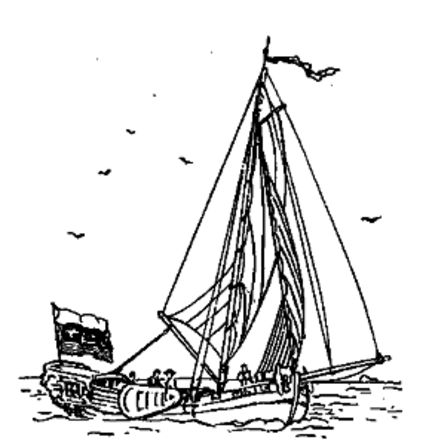
\includegraphics{Yahta_Nevskogo_flota}
\caption{Яхта Невского флота}
\end{wrapfigure}

Возникновение парусного спорта в России связано с именем Петра~I.
Испытывая большую нужду в хорошо обученных матросах и офицерах для
молодого русского флота, Петр~I использовал для подготовки моряков
малые суда.

<<Для увеселения народа, наипаче же для лучшего обучения и искусства
по водам и смелости в плавании>> Петр~I в 1713\,г. учредил в Петербурге
<<Потомственный Невский флот>> \--- прообраз всех современных яхт\-/клубов,
отечественных и зарубежных. Организация Невского флота завершилась
в 1718\,г., когда по указу Петра различным лицам и государственным
учреждениям были розданы гребные лодки\-/верейки, парусные яхты и буера%
\footnote{Так в то время и примерно до середины XIX века назывались небольшие
одномачтовые парусные суда}
с одним лишь условием \--- содержать их в порядке. Все они были построены
на специально созданной для этой цели <<Партикулярной верфи>>. Во главе
Невского флота Петр поставил одного из лучших моряков \--- стольника
Ивана Потемкина, прозванного впоследствии <<Невским адмиралом>>. Невский
флот имел четкую, хорошо продуманную организацию и свои, утвержденные
Адмиралтейств-коллегией, устав и флаг.

Составленный лично Петром~I устав строго регламентировал деятельность
Невского флота, определял обязанности владельцев судов и содержал
наставления по использованию, ремонту и хранению судов и их парусного
вооружения. Были в нем также практические указания по производству
эволюции во время совместного плавания, таблица необходимых сигналов
и т.\,п.

Придавая большое значение деятельности Невского флота, Петр лично
участвовал почти во всех его выходах к Ладоге или к острову Котлин.
После смерти Петра Невский флот распался. Он не был яхт-клубом в современном
понимании. Да и понятия такого тогда не существовало. Но по своей
форме (наличие специально построенных судов, свой флаг и устав, особая
одежда для экипажей судов) и задачам (организация и подготовка людей
для службы на море в сочетании с отдыхом и развлечениями на воде)
Невский флот был прямым предшественником русских и советских яхт-клубов.

Первым официальным русским яхт\-/клубом был основанный в 1846\,г. Императорский
Санкт\-/Петербургский яхт-клуб, в члены которого принимались только
дворяне. 8 июля 1847\,г. Императорский яхт-клуб провел первую в истории
русского парусного спорта гонку яхт. Проходила она по ромбовидной
дистанции в Финском заливе, у Толбухина маяка, по английским правилам
тех лет. Участвовало в этой гонке всего семь яхт: три шхуны и четыре
тендера. В 1849\,г. впервые были проведены гонки по треугольной дистанции,
а в 1852\,г. \--- первая в России международная встреча русских и английских
яхтсменов, победу в которой одержали англичане.{\sloppy\par}

Члены Императорского яхт-клуба ходили и в крейсерские плавания, часто
за пределы Балтийского моря. Наиболее значительными были плавания
лейтенанта Атрыганьева на тендере <<Нереида>> вокруг Европы, из Кронштада
в Николаев и обратно в 1846\==1847 гг. и командора яхт-клуба Лобанова-Ростовского
на шхуне <<Рогнеда>> в Южную Америку в 1851\--1853~гг.

К 1859\,г. активная деятельность Императорского яхт-клуба закончилась.
Постепенно он превратился в фешенебельное собрание высшей аристократии,
не имевшей к спорту никакого отношения.

К этому времени парусным спортом начали увлекаться столичное состоятельное
чиновничество и интеллигенция, которым был закрыт доступ в Императорский
яхт-клуб. В 1858\,г. несколько таких любителей водного спорта организовали
кружок, назвав его <<Моряк на все руки>>. Этот кружок привлек к себе
внимание петербуржцев, и уже в 1859\,г. на его базе была создана спортивная
организация любителей гребного и парусного спорта под названием <<Клуб
Невских ботиков>>. После утверждения в Морском министерстве устава
новый клуб получил официальное наименование <<Санкт-Петербургский Речной
яхт-клуб>> и 21 мая 1860\,г. открыл свой первый спортивный сезон.

Через пять лет Речной яхт-клуб\footnote{Ныне ленинградский яхт-клуб ДСО <<Водник>>}
насчитывал в своем составе около двухсот членов и имел спортивный
флот \--- более 80 гребных и парусных судов. Помимо организации и проведения
гонок Речной яхт-клуб заботился о развитии спортивного судостроения:
созданная в 1864\,г. шлюпочная мастерская яхт-клуба строила самые разнообразные
суда \--- от гребных ботиков до многотонных яхт. 

В 1874\,г. при яхт-клубе были созданы первые в Петербурге Мореходные
классы, которые готовили специалистов для судов торгового флота, а
также корабельных и шлюпочных мастеров. Выпускники получали дипломы
штурманов каботажного и дальнего плавания. Обучение в Мореходных классах
было бесплатным.

В 1875\,г. мастерские яхт-клуба построили первый в России буер <<Метель>>,
положив тем самым начало развитию буерного спорта в стране. 

Большой интерес любителей спорта к деятельности Речного яхт-клуба
побудил его руководителей начать в 1873\,г. издание <<Памятного листка
Санкт\-/Петербургского Речного яхт-клуба>>. Это первое в истории русского
парусного спорта периодическое издание сразу стало популярным и в
следующем, 1874 году было преобразовано в еженедельный журнал <<Яхта>>.
В этом же году яхт-клуб издал <<Сигнальную книжку Санкт-Петербургского
Речного яхт-клуба>> и руководство по парусному спорту <<Моряк-любитель>>
(автор Вандердекен).

Затем появились яхт-клубы и в других речных и приморских городах России,
и к началу девятисотых годов любители занимались парусным спортом
в 68 клубах и обществах. В 90-х годах была предпринята попытка выработать
единые правила для упорядочения спортивной деятельности российских
яхт-клубов. С этой целью в 1897\,г. по инициативе Невского яхт-клуба\footnote{Ныне ленинградский яхт-клуб ВМФ}
был созван <<Первый Всероссийский съезд любителей и деятелей яхтенного
и вообще водного спорта>>. Однако рекомендации и решения съезда ничего
не изменили в узкоместнической практике работы яхт-клубов. Спустя
десять лет петербургский журнал <<Яхта>>, оценивая обстановку того времени,
писал, что все яхт-клубы и парусные общества жили каждый <<своей обособленной
жизнью, на манер отдельных государств\ldots нередко становясь даже в
явно враждебные друг другу отношения>>\footnote{Журнал <<Яхта>>, Спб.. 1908\,г., №54}.

\section{Парусный спорт в Советском Союзе}

\epigraph{\emph{Прошло всего несколько дней. но всем стало уже ясно, что с советскими парусниками приходится считаться, как с первоклассными мастерами.}}{\emph{Газета <<Рома>>. 3 сентября 1960\,г., об олимпийских гонках в Неаполитанском заливе}}

\begin{wrapfigure}{O}{0.5\columnwidth}%
\centering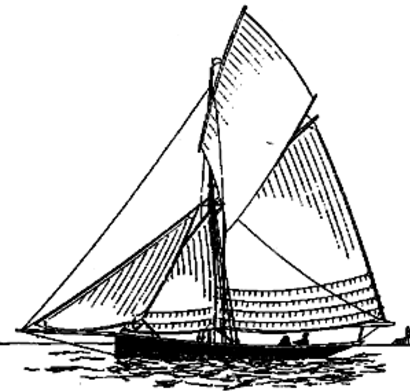
\includegraphics{Gafelnyj_tender_konca_XIX_veka}
\caption{Гафельный тендер XIX века}
\end{wrapfigure}

После Октябрьской революции значительная часть яхтенного флота оказалась
вместе с эмигрировавшими хозяевами за границей, много судов, оставшихся
без надлежащего ухода, погибло или требовало капитального ремонта.
Поэтому в начале 20-х годов энтузиасты- любители взялись за восстановление
парусного флота и хозяйства яхт-клубов. Большую роль в возрождении
парусного спорта сыграло введенное в 1918\,г. всеобщее военное обучение
населения. Молодежь, пополнявшая ряды советского Военно-Морского Флота
и морских территориальных отрядов Всевобуча, знакомилась с морской
службой в яхт-клубах. Активисты Всевобуча пропагандировали парусный
спорт.

Советский парусный спорт получил в наследство сравнительно небольшое
количество яхт. различных и по размерам, и по классам и типам вооружений.
Это очень затрудняло организацию спортивной работы. Из-за недостатка
судов одного класса пришлось вспомнить о гонках с пересадкой рулевых,
которые впервые были проведены в России в 1903\,г. С конца 20-х годов
гонки с пересадкой надолго утвердились в практике советского парусного
спорта.

Несмотря на то что гонки с пересадкой просты в организации, проведение
их обходится достаточно дешево, полностью заменить классные гонки
они не могли. Больше того, увлечение гонками с пересадкой привело
к падению парусной культуры, снижению уровня технической подготовленности
яхтсменов. Поэтому, сыграв положительную роль в строительстве советского
парусного спорта \--- они привлекли к занятиям в яхт-клубах много молодежи,
\--- гонки с пересадкой изжили себя сразу же, как только в стране наладилось
проектирование и строительство классных яхт.

Создание в 1936\,г. Всесоюзной парусной секции\footnote{С 1959\,г. \--- Федерация парусного спорта СССР.}
позволило объединить разрозненную до того времени деятельность яхт-клубов
и парусных секций спортивных обществ и положило начало организованной
и систематической спортивной работе. Были разработаны и введены такие
единые общесоюзные документы, как Правила соревнований, Правила национальной
советской классификации яхт\footnote{Первая попытка создания такой классификации относится к 1929\,г.},
Программы подготовки яхтенных рулевых и Положение об их квалификации.
Первая попытка провести гонки на первенство СССР была предпринята
водным отделом ВСФК в 1924\,г. в Ленинграде на военно-морских шестивесельных
ялах. Несмотря на разосланные приглашения, в гонках приняли участие
только ленинградские яхтсмены и моряки Балтийского флота. Выиграл
первенство экипаж шлюпки спортклуба <<Спартак>> (рулевой Б.\,Б.~Лобач\-/Жученко).

Яхтсмены разных городов встретились в 1928\,г. на I Всесоюзной спартакиаде.
Победителям гонок на этой спартакиаде \--- кронштадтцу А.\,К.~Бальсевичу
(килевые яхты) и представителю Самары Н.\,А.~Мясникову (швертботы) \--- впервые было присвоено звание чемпионов СССР по парусному спорту.

Соревнования на первенство СССР по парусному спорту стали проводиться
с 1936\,г. Два первенства, проведенные до войны (1936 и 1938~гг.),
во многом способствовали развитию парусного спорта в стране.

Большое значение для развития парусного спорта имело его возрождение в
Москве. Вначале московский яхтенный флот составляли несколько швертботов,
которые в 1937\,г. перегнала в столицу группа ленинградских яхтсменов.
А в 1938\,г. в Москве было уже более 100 швертботов, четыре яхт-клуба
и более четырехсот яхтсменов, актив которых составил ядро Всесоюзной
парусной секции.

К началу 40-х годов парусным спортом в СССР занимались уже тысячи
спортсменов. В составе спортивного флота появилось много яхт, построенных
по Правилам классификации 1936\,г.: килевые крейсерско-гоночные яхты
классов Л-45, Л-60 и Л-100, швертботы для озерного и прибрежного морского
плавания класса М-20, речные гоночные швертботы классов Р-20, Р-30
и Р-45, швертботы-одиночки класса Ш-10. Все эти суда были сконструированы
и построены в Ленинграде, Горьком, Куйбышеве. Яхт-клубы Ленинграда,
Одессы, Николаева, речные яхт-клубы Москвы, Саратова, Перми, яхт-клубы ВМФ в Кронштадте и Севастополе воспитали немало отличных яхтсменов:
И. Матвеева, Р. Алексеева, С. Зимина, П. Якшарова, Е. Сахарову и многих
других. Спортивно-массовая работа предвоенных лет не прошла бесследно.
Многие яхтсмены, в частности ленинградские, в годы Великой Отечественной
войны успешно воевали на катерах МО и торпедных катерах. Большую помощь
осажденному Ленинграду оказали яхтсмены\-/буеристы \--- они участвовали в
создании ледовой <<дороги жизни>> на Ладожском озере и в организации
дозорной службы и связи между сигнально-наблюдательными постами на
льду Финского залива.

Развитие советского парусного спорта после окончания Великой Отечественной
войны шло стремительным темпом. Довоенный яхтенный флот был не только
восстановлен, но значительно пополнен судами новых национальных и
международных классов. Уже в 1945\,г. было проведено первенство СССР.
Включились в активную работу яхт-клубы Прибалтики; яхтенное судостроение
получило новую базу \--- экспериментальную спортивную судоверфь в Таллине.
Большое значение имел переход к Международным правилам гонок, начатый
еще в 1939\,г. и завершенный в 1952\,г. Он существенно облегчил нашим
яхтсменам участие в международных состязаниях.

В 1952\,г. советские яхтсмены впервые приняли участие в Олимпийских
играх. Однако выступление на XV Олимпиаде в Хельсинки было крайне
неудачным: в двух классах наши яхтсмены заняли последние места, в
трех остальных \--- близкие к последним. Анализ причин этой неудачи заставил
коренным образом изменить систему учебно-воспитательной работы в
парусном спорте. Начиная с 1953\,г. все парусные соревнования стали
проводиться как классные гонки, кроме клубных, где еще рекомендовались
гонки с пересадкой. Больше внимания стало уделяться организации встреч
советских яхтсменов с зарубежными. Так, в 1954\,г. состоялась встреча
Финляндия \--- СССР, а в 1955\,г. \--- Швеция \--- СССР. Советские яхтсмены
участвовали в ряде регат, проводившихся в Швеции, Финляндии, ГДР,
и к XVI Олимпийским играм в 1956\,г. приобрели некоторый опыт международных
встреч. И хотя наши экипажи все еще отставали от лучших зарубежных
гонщиков, выступление команды СССР на Олимпиаде в Мельбурне было более
успешным, чем в Хельсинки. 

Готовясь к XVII Олимпиаде, советские яхтсмены приложили много усилий,
чтобы устранить недостатки прошлых лет. Были значительно повышены
требования к спортивной подготовке гонщиков на яхтах международных
классов, улучшился и значительно вырос спортивный флот, подготовка
ведущих яхтсменов достигла уровня международного класса.

Способность советских парусников достойно представлять свою страну
за рубежом подтвердилась результатами олимпийских гонок в Неаполитанском
заливе в 1960\,г. Наши яхтсмены заняли первое место в классе <<Звездный>>
(рулевой Т.~Пинегин, шкотовый Ф.~Шутков), второе \--- в классе швертботов-одиночек
<<Финн>> (рулевой А.~Чучелов) и зачетное шестое в классе швертботов
<<Летучий голландец>> (рулевой А.~Шелковников, шкотовый В.~Пильчин).
Несмотря на слабые результаты в классах <<Дракон>> (16-е место) и <<5,5-метровом>>
(14-е место), команда СССР уверенно заняла второе место в неофициальном
командном зачете, уступив первое команде Дании. На Олимпиаде в Токио
в 1964\,г. наши яхтсмены выступили неудачно главным образом из-за аварий
и неполадок в материальной части. Олимпийские игры в Мехико вновь
принесли победу представителю советской команды \--- рулевой швертбота
<<Финн>> В. Манкин завоевал золотую медаль в гонках в заливе Акапулько.

Хороших результатов добились советские яхтсмены в гонках на XX Олимпиаде
в 1972\,г. Рулевой В. Манкин и шкотовый В. Дырдыра выиграли золотую
медаль в классе <<Темпест>>, а В. Потапов \--- серебряную в классе <<Финн>>.
В десятку сильнейших вошли наши гонщики в классах <<Летучий голландец>>
(6-е место), <<Солинг>> (7-е место) и <<Звездный>> (9-е место).

Не менее успешно развиваются в нашей стране и крейсерские плавания.
Уже в 20-х годах яхтсмены Ленинграда совершали одиночные и совместные
плавания в Ладожское озеро и Балтийское море, в порты Эстонии, Финляндии,
Германии, Латвии. В 1931\,г. одесские яхтсмены на яхте <<Комсомолец>>
предприняли плавание в Стамбул. Николаевские парусники на крейсерской
яхте <<Арктика>> в 1938\,г. прошли 2500 миль. Наиболее интересными в
30-х годах были плавания ленинградских яхт <<Ударник>> и <<Пионер>> вокруг
Скандинавии и яхты <<Стахановец>>\footnote{Ныне яхта <<Россия>>, учебное судно ленинградского яхт-клубр, ДСО <<Труд>>.}
в Белое море. Руководили этими походами известные яхтенные капитаны
В.\,Г. Щепкин, Г.\,Ф.~Гефдинг и И. П. Матвеев В послевоенные годы крейсерские
плавания и маршрутные гонки прочно утвердились в работе яхт-клубов.
В 50\--60-х годах советские яхтсмены выходили в плавания в отечественные
морские и внутренние воды, ходили и за границу, посещали порты братских
социалистических стран \--- Польши, ГДР, Болгарии, Румынии, участвовали
в крейсерских гонках за рубежом, в частности в Варнемюндских регатах.
Большую популярность приобрели крейсерские гонки <<Мухувяйнская неделя>>
в Эстонии и гонки на Кубок Балтийского моря, в которых участвует большое
число яхт. А летом 1971\,г. ленинградские яхтсмены вновь после долгого
перерыва вышли в океан и на яхте <<Сатурн>> (капитан В. Н. Дерябин,
яхт-клуб ВМФ) за 25 суток ходового времени обошли вокруг Скандинавского
полуострова. 

Советский парусный спорт еще молод. Наиболее развит он в РСФСР, особенно
в Москве и Ленинграде, в Латвии, Эстонии и на Украине. Выросли коллективы
яхтсменов и там, где до революции о парусном спорте не знали вообще \--- в республиках Закавказья и Средней Азии, в городах Сибири и Дальнего
Востока.

С тех пор, как рабочий класс стал хозяином своей страны, полностью
изменилось лицо парусного спорта в СССР, изменился и неизмеримо вырос
контингент яхтсменов. Вместо сотен аристократов и буржуа \--- тысячи
рабочих и служащих, юношей и девушек участвуют в гонках и крейсерских
плаваниях, в работе яхт-клубов и спортивных секций в наше время.

Организационной формой советского парусного спорта является секция,
работающая на базе яхт-клуба или водной станции ДСО, ведомства или
города, которые обеспечивают стоянку, хранение и эксплуатацию яхт,
а также ведут учебно-спортивную работу членов секции. Общественное
руководство учебно-спортивной работой парусных секций, организацию
и проведение соревнований осуществляют городские федерации парусного
спорта. В союзных республиках, культивирующих парусный спорт, в Москве
и Ленинграде организованы республиканские федерации, работающие под
руководством Федерации парусного спорта СССР и республиканских комитетов
по физкультуре и спорту. В 1956\,г. Федерация парусного спорта СССР
вступила в члены Международного союза парусных соревнований (ИЯРУ).
Представитель СССР является членом Постоянного комитета этого союза.

\section{Парусный спорт за рубежом}
\epigraph{\emph{Молодым людям, замышляющим такое плавание, я скажу: <<Отправляйтесь!>>}}{\emph{Дж. Слокам, <<Один под парусами вокруг света>>}}

\begin{wrapfigure}{O}{0.5\columnwidth}
\centering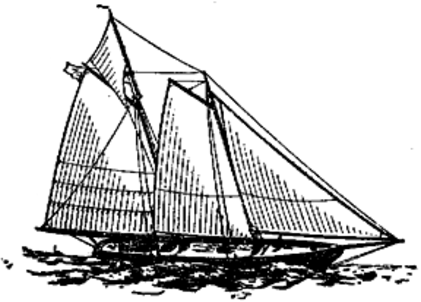
\includegraphics{Amerika}
\protect\caption{<<Америка>> \--- самая быстроходная яхта середины XIX века}
\end{wrapfigure}

За рубежом парусный спорт возник раньше всего в странах с развитым
мореплаванием \--- в Англии и Голландии. Зарождение его тесно связано
с профессиональным плаванием на небольших парусных судах, где преимущество
в скорости позволяло успешно конкурировать, например, в рыболовстве
или лоцманской службе. Спортивный интерес, возникший в процессе улучшения
ходовых качеств таких судов, проведение гонок между ними привели к
созданию специальных судов, предназначенных только для любительского
плавания, которые стали называться яхтами\footnote{От голландского слова <<jagte>> \--- так в Голландии в XVII веке называли
небольшие быстроходные одномачтовые суда}.

Со временем число владельцев яхт, в большинстве своем уже ничего общего
не имеющих со службой на море, возросло настолько, что появилась потребность
в создании специальных объединений любителей парусного спорта \--- яхт-клубов.
По данным известного в дореволюционной России яхтсмена Г.\,В.~Эша,
автора популярного <<Руководства для любителей парусного спорта>>, рождение
парусного спорта за рубежом можно датировать 1662 годом, когда в английском
городе Вульвиче состоялись первые в мире официальные гонки между яхтой
короля Карла~II и голландской шхуной. Победу одержали англичане. С
этого времени состязания между отдельными владельцами яхт стали проводиться
вначале в Англии, а затем и в других странах Западной Европы и Америки.

Первичные организации яхтсменов за рубежом \--- яхт\-/клубы \--- появились
в Англии в 1720\,г., когда в ирландском городе Корке был учрежден <<Водный
клуб коркской гавани>>, первый европейский яхт-клуб, вскоре, однако,
распавшийся. Свое современное название общества яхтсменов получили
от организованного в 1810\,г. в английском городе Коусе <<Яхт-Клуба>>.
Число английских яхт-клубов росло довольно быстро. Ставя перед собой
чисто спортивные задачи, они организовывали самые различные гонки,
вплоть до крейсерских гонок вокруг Британских островов.{\sloppy\par}

В США первый яхт\-/клуб появился в 1811\,г. в Нью-Йорке. В 1832\,г. был
создан первый шведский яхт\-/клуб в Стокгольме, в 1835\,г. \--- яхт\-/клуб
в Берлине, в 1838\,г. \--- гоночное общество в Гавре. К концу XIX века в
Европе насчитывалось уже более двухсот яхт\-/клубов.

Росло и число яхтсменов. Парусный спорт из чисто аристократического
занятия, каким он был в период своего зарождения, постепенно превращался
в спорт относительно массовый.

Правда, большинство любителей могли рассчитывать только на приобретение
старых, вышедших из класса судов. Но именно это и послужило толчком
к созданию дешевых в постройке и сравнительно простых по конструкции
яхт \--- гоночных и крейсерских яхт\-/монотипов серийной постройки, стоимость
которых много меньше стоимости яхт формульных классов штучной постройки.

С 1900\,г. парусный спорт вошел в программу Олимпийских игр, а в 1907\,г.
начал свою деятельность Международный союз парусных соревнований (ИЯРУ).
С созданием этого Союза появилась возможность для организации и проведения
международных встреч: была разработана единая классификация яхт и
единые правила гонок. С 1948\,г. под контроль ИЯРУ полностью взята
и организация олимпийских парусных гонок. Кроме ИЯРУ делами парусного
спорта за рубежом занимаются еще и международные ассоциации яхт отдельных
классов, регулирующие правила этих классов, проведение в этих классах
первенств мира и континентов, регистрирующие яхты. Объединяя владельцев
яхт одного класса, эти ассоциации управляют делами классов <<Звездный>>,
<<Дракон>>, <<Финн>>, <<Летучий голландец>> и др. 

К настоящему времени наибольшего развития зарубежный парусный спорт
достиг в США, Англии, Дании, Швеции, Норвегии, ФРГ, Италии, Аргентине,
Австралии, Финляндии, Франции. Успешно развивается он и в социалистических
странах: Польше, Венгрии, Болгарии, Чехословакии и ГДР. 

В странах, где наиболее развит парусный спорт, наравне с международными
классами культивируются многочисленные национальные классы яхт и швертботов;
в странах, где он менее развит, \--- в основном международные классы
и национальные классы соседних стран.

Широко распространены за рубежом и маршрутные гонки на длинные дистанции,
часто океанские, и дальние плавания на яхтах не только в свои порты,
но и трансокеанские и кругосветные. Наибольшей известностью пользуются
Бермудская гонка из Ньюпорта (США) до Бермудских островов, гонки из
Торбея (Англия) до Лиссабона (Португалия), гонки яхтсменов Балтики
вокруг острова Готланд, гонки через Атлантику из Англии в США.

Среди крейсерских океанских и кругосветных плаваний на яхтах широко
известны плавания американца Дж. Слокама (1895\--1898~гг.), француза
А.~Жербо (1923\--1929~гг.), англичанина Ф. Чичестера (1966\--1967~гг.),
поляка Л.~Телиги (1966\--1969~гг.), которые совершили свои путешествия
в одиночку.

Самыми интересными современными крейсерскими гонками были гонки яхтсменов\-/одиночек вокруг света без захода в порты. Организованы они были в
1968\,г. английской газетой <<Санди Таймс>> и закончились победой англичанина
Р. Нокс-Джонсона, затратившего на гонку 310 ходовых суток и выигравшего
приз <<Золотой глобус>>.


\section{Что такое парусный спорт}

\epigraph{\emph{Что может лучше олицетворять... отвагу и дерзновенность человека, чем крохотный белоснежный парус, затерявшийся в волнующемся просторе моря, смело стремящийся, невзирая на все препятствия, к своей цели!}}{\emph{М. Баринов, <<Бегущая по волнам>>}\footnote{Из сборника <<Песня о парусе>>. ФиС, 1962.}}

\begin{wrapfigure}{O}{0.5\columnwidth}
\centering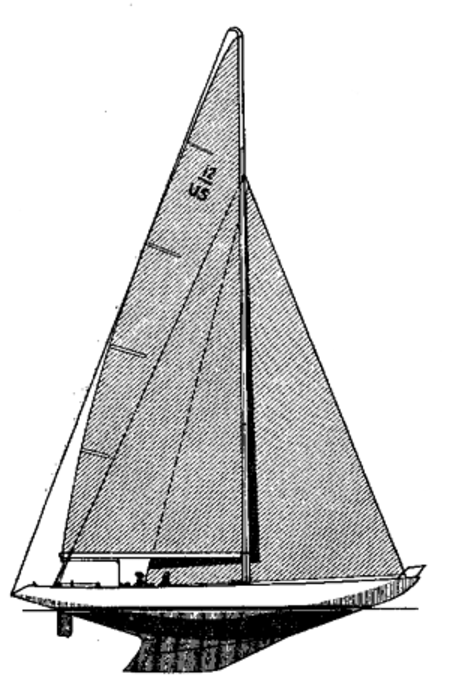
\includegraphics[scale=1]{Yachta_12-metrovogo_mezhdunarodnogo_klassa}
\protect\caption{Яхта 12-метрового международного класса}
\end{wrapfigure}

Парусный спорт \--- один из тех немногочисленных видов спорта, занимаясь
которым человек не только соревнуется в мастерстве с другими яхтсменами,
но и сталкивается лицом к лицу с силами природы.

В борьбе со стихией спортсмен развивается физически, становится выносливым
и закаленным. Плавания на яхтах, будь то гонка или крейсерское плавание,
как и занятия, например, альпинизмом или планерным спортом, способствуют
воспитанию таких черт характера, как смелость и решительность, находчивость
и инициатива, воля к победе. В парусном спорте особенно ярко проявляются
черты коллективизма, так как если в яхтенном экипаже нет сплоченности,
гонка наверняка закончится поражением. Поэтому в каждом яхтсмене,
от матроса до капитана яхты, должны быть развиты чувства личной ответственности,
разумной и строгой дисциплины, подлинного товарищества и взаимопомощи.

Велико и прикладное значение парусного спорта. Наряду с высокими физическими
и моральными качествами каждый яхтсмен, в зависимости от своей квалификации,
непременно должен обладать комплексом специальных знаний, быть хорошо
подготовленным к грамотному и умелому управлению яхтой при любой погоде,
к содержанию судна и его вооружения в хорошем состоянии.

Поскольку парусный спорт \--- это не только гонки на ограниченной дистанции,
но и длительные крейсерские гонки, и дальние плавания на яхтах, яхтсмен
должен также иметь определенные знания в области судовождения, морской
практики, метеорологии и других морских наук. А чтобы хорошо подготовить
яхту к выходу в плавание, нужно знать столярное и малярное дело, владеть
слесарным и такелажным инструментом. Поэтому трудно переоценить значение
парусного спорта как хорошей школы начальной морской подготовки.

И, наконец, в парусном спорте, как нигде, на человека активно воздействуют
три основных оздоровительных фактора \--- солнце, свежий воздух и вода.
Они способствуют закаливанию организма и создают отличные условия
для превосходного активного отдыха.

Вместе с тем парусный спорт требует не только глубоких теоретических
знании, но и умения использовать их на практике.

Если неумение владеть шайбой или мячом в спортивных играх в самом
худшем случае приводит к проигрышу матча, то неопытный или плохо знающий
свое дело яхтенный рулевой может стать виновником аварии, опасной
не только для него самого, но и для его экипажа и окружающих судов
и людей. К сожалению, в практике парусного спорта зафиксировано немало
печальных случаев, когда в результате неумелого управления яхтой или
грубого нарушения правил хорошей морской практики выходы в море или
гонки заканчивались тяжелыми авариями яхт, нередко сопровождающимися
гибелью судов и человеческими жертвами. Поэтому помимо овладения спортивным
мастерством каждый яхтсмен, яхтенный рулевой или капитан должен получить
официальное свидетельство или диплом, подтверждающие его квалификацию
и дающие право управлять яхтой, точно так же, как шоферу \--- водить
автомобиль, пилоту \--- держать в руках штурвал самолета и т.\,д.

Каждый яхтсмен должен прежде всего стать настоящим моряком, а это
значит \--- уметь применять полученные знания и на гоночной дистанции
и в дальнем крейсерском плавании.

%===========================================================================
%
%                          Классификация парусных яхт
%
%===========================================================================

\chapter{Классификация парусных яхт}

%--------------------------------------------------------------------------
%
%                             Основные части яхты
%
%--------------------------------------------------------------------------

\section{Основные части яхты}

Яхтой называется всякое судно, безразлично \--- моторное или парусное,
предназначенное для спортивных или туристских целей. Парусная яхта
имеет две главные части: \textbf{корпус\index{корпус}} и вооружение.
Корпус предназначен для размещения экипажа и предметов снабжения яхты.
Под \textbf{вооружением\index{вооружение}} понимают паруса
и все устройства для установки парусов и управления ими.

Рассмотрим основные части корпуса парусной яхты (рис.~\ref{fig:1}).
Передняя часть корпуса называется \textbf{носом}\index{нос}, задняя
\--- \textbf{кормой}\index{корма}. Части корпуса, нависающие над
водой, носят название носового и кормового \textbf{свесов}\index{свес};
боковые поверхности корпуса \--- \textbf{бортов}\index{борт}. Правый
и левый борта определяются, если смотреть с кормы на нос. Нижняя поверхность
корпуса называется \textbf{днищем}\index{днище}, переход от
борта к днищу \---\textbf{скулой}\index{скула}. Задний обрез корпуса
носит название транец, обращенная к воде поверхность кормового свеса \---
\textbf{подзор}\index{подзор}. Сверху корпус закрывается \textbf{палубой}\index{палуба},
предохраняющей судно от попадания воды внутрь. Палуба \--- это вообще
всякий настил, прикрывающий какое-либо расположенное ниже помещение.
Носовая часть палубы называется \textbf{баком}\index{бак}, кормовая
\--- \textbf{ютом}\index{ют}, средняя \--- \textbf{шканцами}\index{шканцы}\footnote{Название <<шканцы>> не принято применять на малых яхтах, но на яхтах
длиной более 14\--15 м оно вполне уместно.}.

\begin{figure}[htbp]
\centering
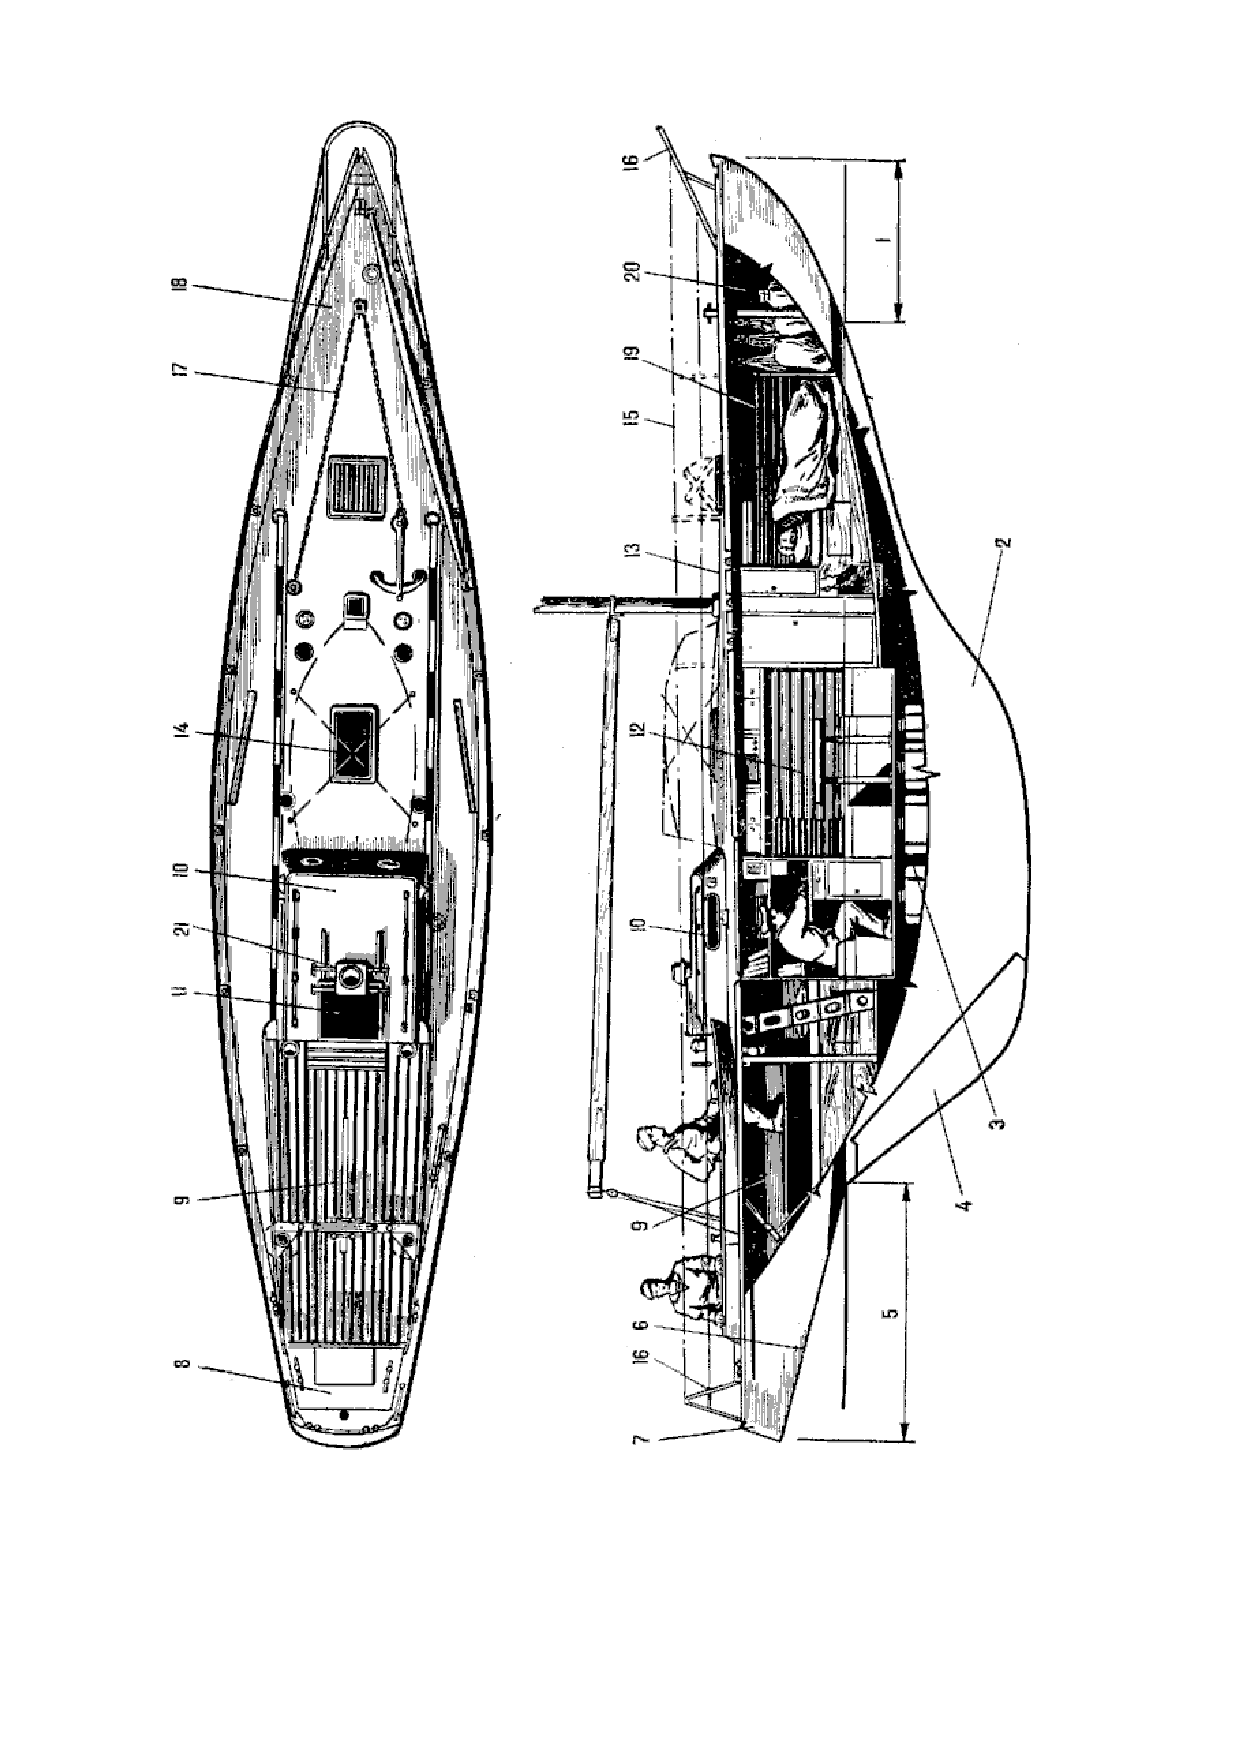
\includegraphics[scale=0.9]{Kilevaya_yachta_i_ee_chasti}
\par
\protect\caption{\label{fig:1}Килевая
яхта и её части}
\centering{}\small 1~---~носовой свес; 2~---~киль; 3~---~трюм; 4~---~перо
руля; 5~---~кормовой свес; 6~---~подзор; 7~---~транец; 8~---~ют; 9~---~кокпит;
10~---~рубка; 11~---~входной люк; 12~---~каюта; 13~---~палуба; 14~---~световой
(светлый) люк; 15~---~леерное ограждение, 16~---~носовой в кормовой
релинги; 17~--- якорное устройство (якорь, день, битенг, палубный клюз),
18 --- бак; 19 --- кубрик; 20 --- форпик; 21 --- компас.
\end{figure}

В палубе для размещения экипажа делаются вырезы \--- \textbf{кокпиты}\index{кокпит}.
Кокпиты бывают открытыми, когда они не отгорожены от подпалубного
пространства, и закрытыми. В последнем случае они представляют собой
ящик, вставленный в вырез палубы и изолированный от под-палубного
пространства. Закрытый кокпит обычно делают самоотливным, располагая
его пол выше ватерлинии и оборудуя сливными трубами. Через эти трубы
вода, попавшая в кокпит с палубы, сливается за борт. Самоотливными
кокпиты бывают на морских яхтах, у которых возможно попадание на палубу
больших количеств воды, а также на современных гоночных швертботах.
Правда, у последних самоотливной кокпит имеет слив воды не через трубы,
а через клапан или просто отверстия в транце, прорезанные на уровне
глухого пола кокпита.

Нижняя часть подпалубного пространства, расположенная под полом каюты
или кокпита, называется \textbf{трюмом}\index{трюм}. Трюм закрывается
настилом, который носит название \textbf{сланей\index{слань}}
или \textbf{пайол}\index{пайол}. Поперечными переборками (стенками)
корпус яхты делится на помещения \--- \textbf{отсеки}\index{отсек}.

Жилые помещения на яхте называются \textbf{каютами}\index{каюта};
каюта, расположенная под баком,\--- \textbf{кубриком}\index{кубрик},
крайние носовой и кормовой отсеки корпуса \--- соответственно \textbf{форпиком\index{форпик}}
и \textbf{ахтерпиком}\index{ахтерпик}.

Отверстия в палубе для сообщения с подпалубным пространством называют
\textbf{люками}\index{люк}. Различают входные и световые (светлые)
люки, крышки которых обычно застеклены.

Если высота подпалубного пространства недостаточна, то на палубе делают
\textbf{надстройки}\index{надстройка}. Надстройка над каютой
называется \textbf{рубкой}\index{рубка}. В стенках рубки (комингсах)
вырезают окна \--- \textbf{иллюминаторы}\index{иллюминатор}.

Бытовые помещения на яхте, как и на большом корабле, имеют свои названия:
кухня \--- \textbf{камбуз}\index{камбуз}, уборная \---\textbf{гальюн}\index{гальюн}.

Для управления яхтой служит руль, поворачиваемый \textbf{румпелем}\index{румпель}.
Часть руля, к которой крепится румпель (или другой рулевой привод),
называется \textbf{головкой\index{головка руля} }руля.

Основные части вооружения яхты \--- паруса, рангоут и такелаж. Паруса
\--- основной движитель яхты. Они делятся на три комплекта: основные
(или лавировочные), дополнительные и штормовые паруса.

\textbf{Основные паруса\index{паруса!основные}} яхта
несет в обычных плаваниях. Эти же паруса определяют обмерную площадь
парусности яхты.

Участие в гонках требует особых парусов, увеличивающих площадь парусности
в некоторых ситуациях, возникающих на дистанции (например, при попутных
ветрах). Такие паруса называют \textbf{дополнительными}\index{паруса!дополнительные}.

При плавании в штормовую погоду лавировочные паруса заменяют меньшими
по размерам и более прочными \textbf{штормовыми парусами}\index{паруса!штормовые}.

Совокупность всех деревянных или металлических частей вооружения,
служащих для крепления и несения парусов, называется \textbf{рангоутом}\index{рангоут}. 

\textbf{Такелаж}\index{такелаж} \--- снасти, изготовленные из
растительного или стального троса, \--- подразделяют на стоячий и бегучий.
\textbf{Стоячий такелаж}\index{такелаж!стоячий} служит
для расчалки и поддержания в рабочем положении рангоута, а \textbf{бегучий}\index{такелаж!бегучий}
\--- для постановки и уборки парусов и рангоута, управления парусами,
для подъема и спуска сигналов.

Подробно на устройстве парусов, рангоута и такелажа мы остановимся
в разделе \emph{<<Устройство и вооружение яхты>>}.

%--------------------------------------------------------------------------
%
%                             Типы парусных яхт
%
%--------------------------------------------------------------------------

\section{Типы парусных яхт}

В практике парусного спорта используются яхты самых различных видов
и размеров. В зависимости от условий плавания в том или ином районе
применяют большие или меньшие яхты той или иной конструкции. Тип яхты
в первую очередь определяется её назначением и районом плавания, а
также конструкцией корпуса и вооружения.

По этому признаку различают крейсерские и гоночные яхты. Основное
назначение \textbf{гоночных яхт}\index{яхта!гоночная}
\--- парусные гонки на ограниченных дистанциях, поэтому их строят предельно
легкими. Для дальних плаваний они недостаточно прочны и не имеют бытовых
удобств.

\textbf{Крейсерские яхты}\index{яхта!крейсерская},
наоборот, имеют очень прочную конструкцию и максимум бытовых удобств,
то есть отвечают своему основному назначению \--- крейсерским плаваниям
и гонкам в открытом море с большим удалением от базы.

В современном парусном спорте чисто крейсерские яхты мало распространены.
Имеется большое количество яхт для участия в морских гонках, которые
называют \textbf{крейсерско-гоночными}\index{яхта!крейсерско-гоночная}.
Такие яхты пригодны и для дальних плаваний, вплоть до океанских.

Крейсерские и крейсерско\-/гоночные яхты снабжены необходимым штурманско\-/навигационным оборудованием и, как правило, вспомогательным двигателем.

Кроме такой общей классификации существует еще спортивная классификация
яхт, определяющая разделение их на классы.

\textbf{Спортивная классификация}\index{спортивная классификация}
яхт необходима для создания равных условий спортивной борьбы в гонках.
В рамках каждого класса по возможности обеспечиваются равные шансы
на выигрыш соревнования (в той мере, в какой эти шансы определяются
самой яхтой).

В каждом классе форма и размеры яхты в большей или меньшей степени
ограничены, с тем чтобы яхты данного класса имели по возможности одинаковую
быстроходность и наилучшие мореходные качества.

%--------------------------------------------------------------------------
%
%                       Различия яхт по форме корпуса
%
%--------------------------------------------------------------------------

\section{Различия яхт по форме корпуса}

Особенности конструкции корпуса парусной яхты определяются применением
на ней паруса в качестве основного движителя.

\begin{wrapfigure}{O}{0.5\columnwidth}%
\centering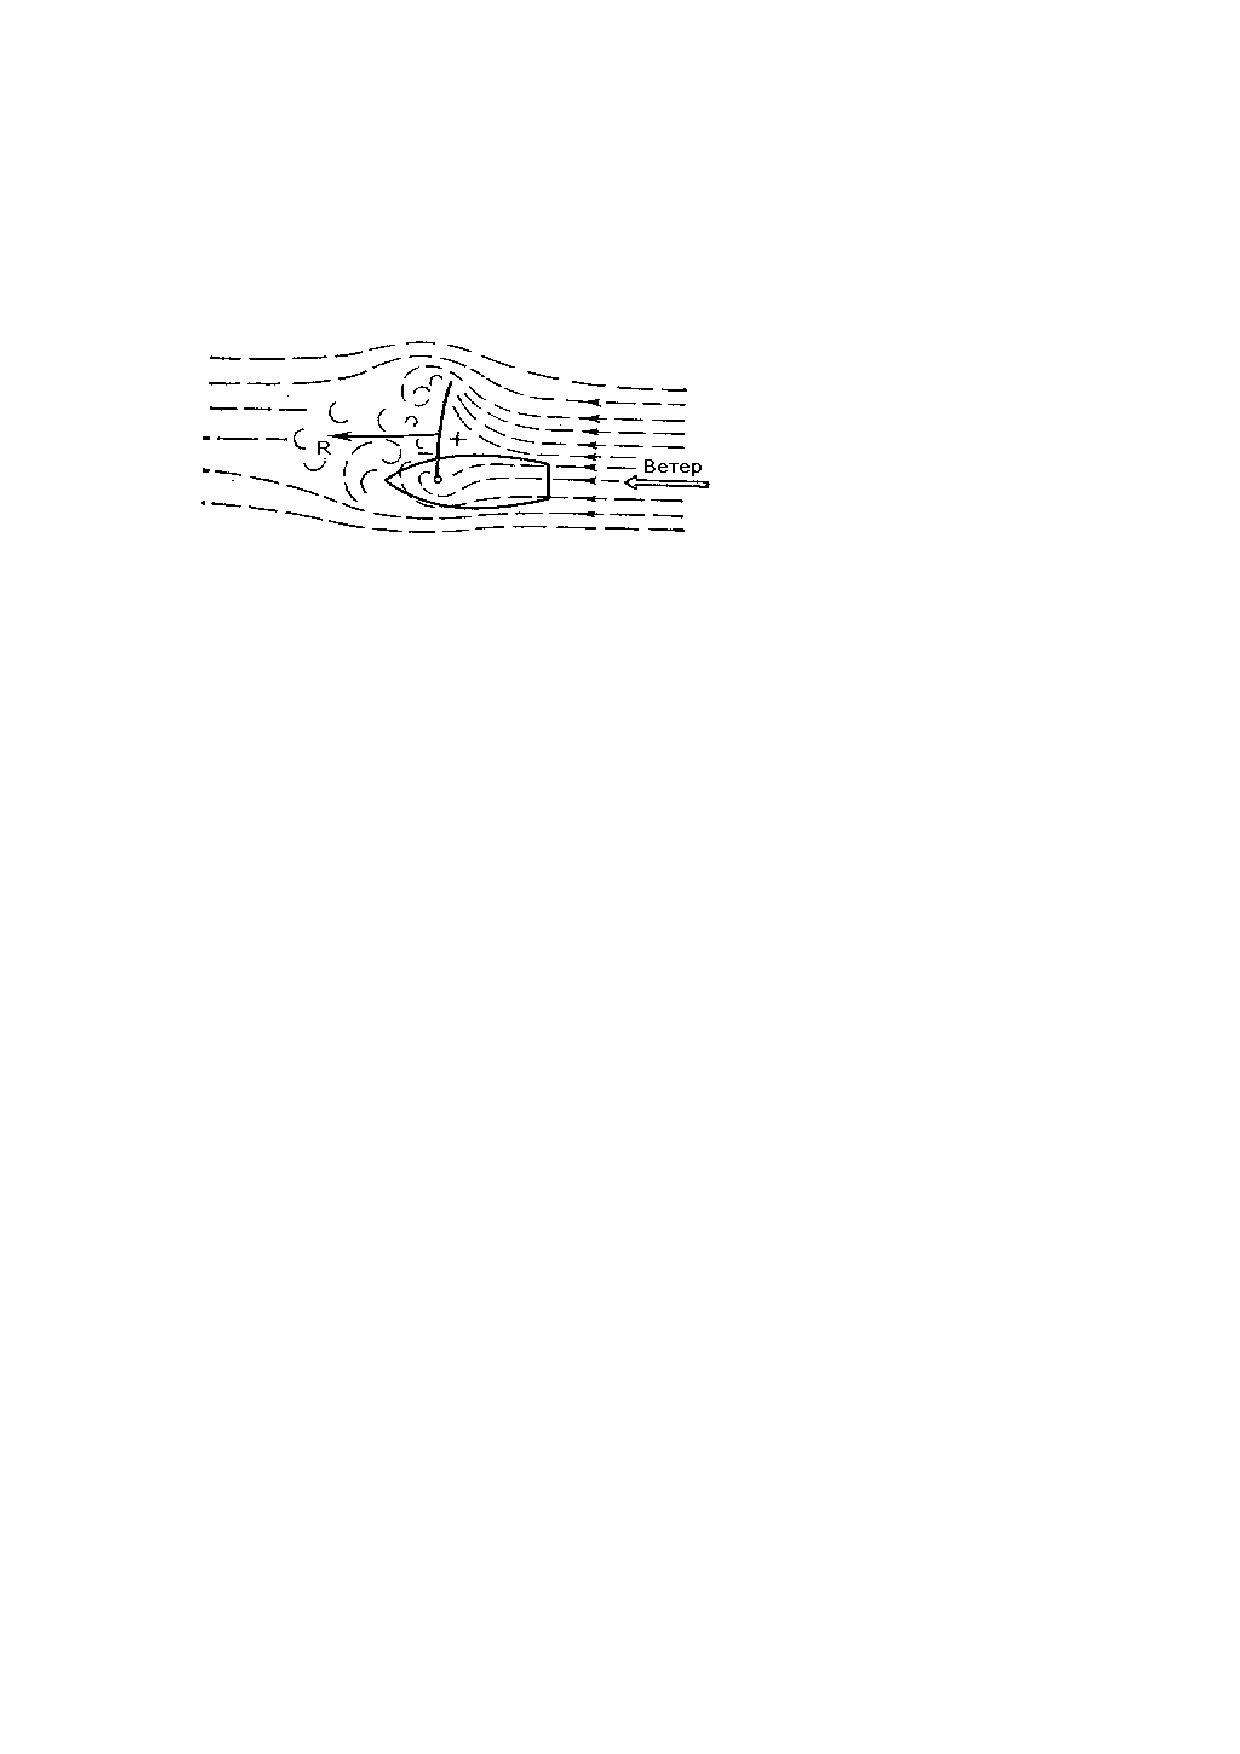
\includegraphics[scale=1]{Deystvie_poputnogo_vetra}
\protect\caption{\label{fig:Deystvie_poputnogo_vetra}Действие
ветра на паруса яхты, идущей попутным ветром}
\end{wrapfigure}%

Представим себе, что ветер дует прямо в корму яхте (рис.~\ref{fig:Deystvie_poputnogo_vetra}).
Струи воздуха, набегая на парус, создают определенное давление на
его наветренную сторону. Огибая парус, струи стремятся уйти (вместе
со всем движущимся воздухом) дальше, вследствие чего на подветренной
стороне паруса создается некоторое разрежение. В результате одновременного
давления на наветренной стороне паруса и разрежения на подветренной
его стороне возникает сила давления ветра на парус. Она-то и тянет
его, а вместе с ним и яхту по направлению движения (если парус стоит
как нарисовано, перпендикулярно ветру). Это наиболее простой случай.

Другое дело, когда яхта идет так, что ветер дует под углом к направлению
ее движения (рис.~\ref{fig:Deystvie_vetra_ostryy_ugol}).
Тогда сила $\overrightarrow{R}$ давления ветра на парус, очевидно, не будет
совпадать с направлением движения яхты. Экспериментально выяснено,
что она направлена примерно перпендикулярно к плоскости паруса.

Эта сила будет вызывать не только движение судна вперед, но и в значительной
мере снос его в сторону, или, как говорят, дрейф под ветер.

Можно разложить силу $\overrightarrow{R}$ по правилу параллелограмма на две силы,
направленные соответственно по направлению движения яхты и перпендикулярно
ему. Полученная в результате разложения сила $\overrightarrow{T}$ будет тянуть
судно по направлению его движения. Называют её \textbf{силой тяги\index{сила тяги}}.
Сила $\overrightarrow{D}$ вызывает снос (дрейф) судна в сторону и поэтому называется
\textbf{силой дрейфа\index{сила дрейфа}}. Наличие этих
двух сил, возникающих в результате давления ветра на паруса, определяют
те особенности, о которых мы уже говорили. В самом деле, суда другого
типа (паровые, моторные, буксируемые) в нормальных условиях не имеют
силы дрейфа, вызываемой их движителем.

\begin{wrapfigure}{O}{0.5\columnwidth}%
\centering
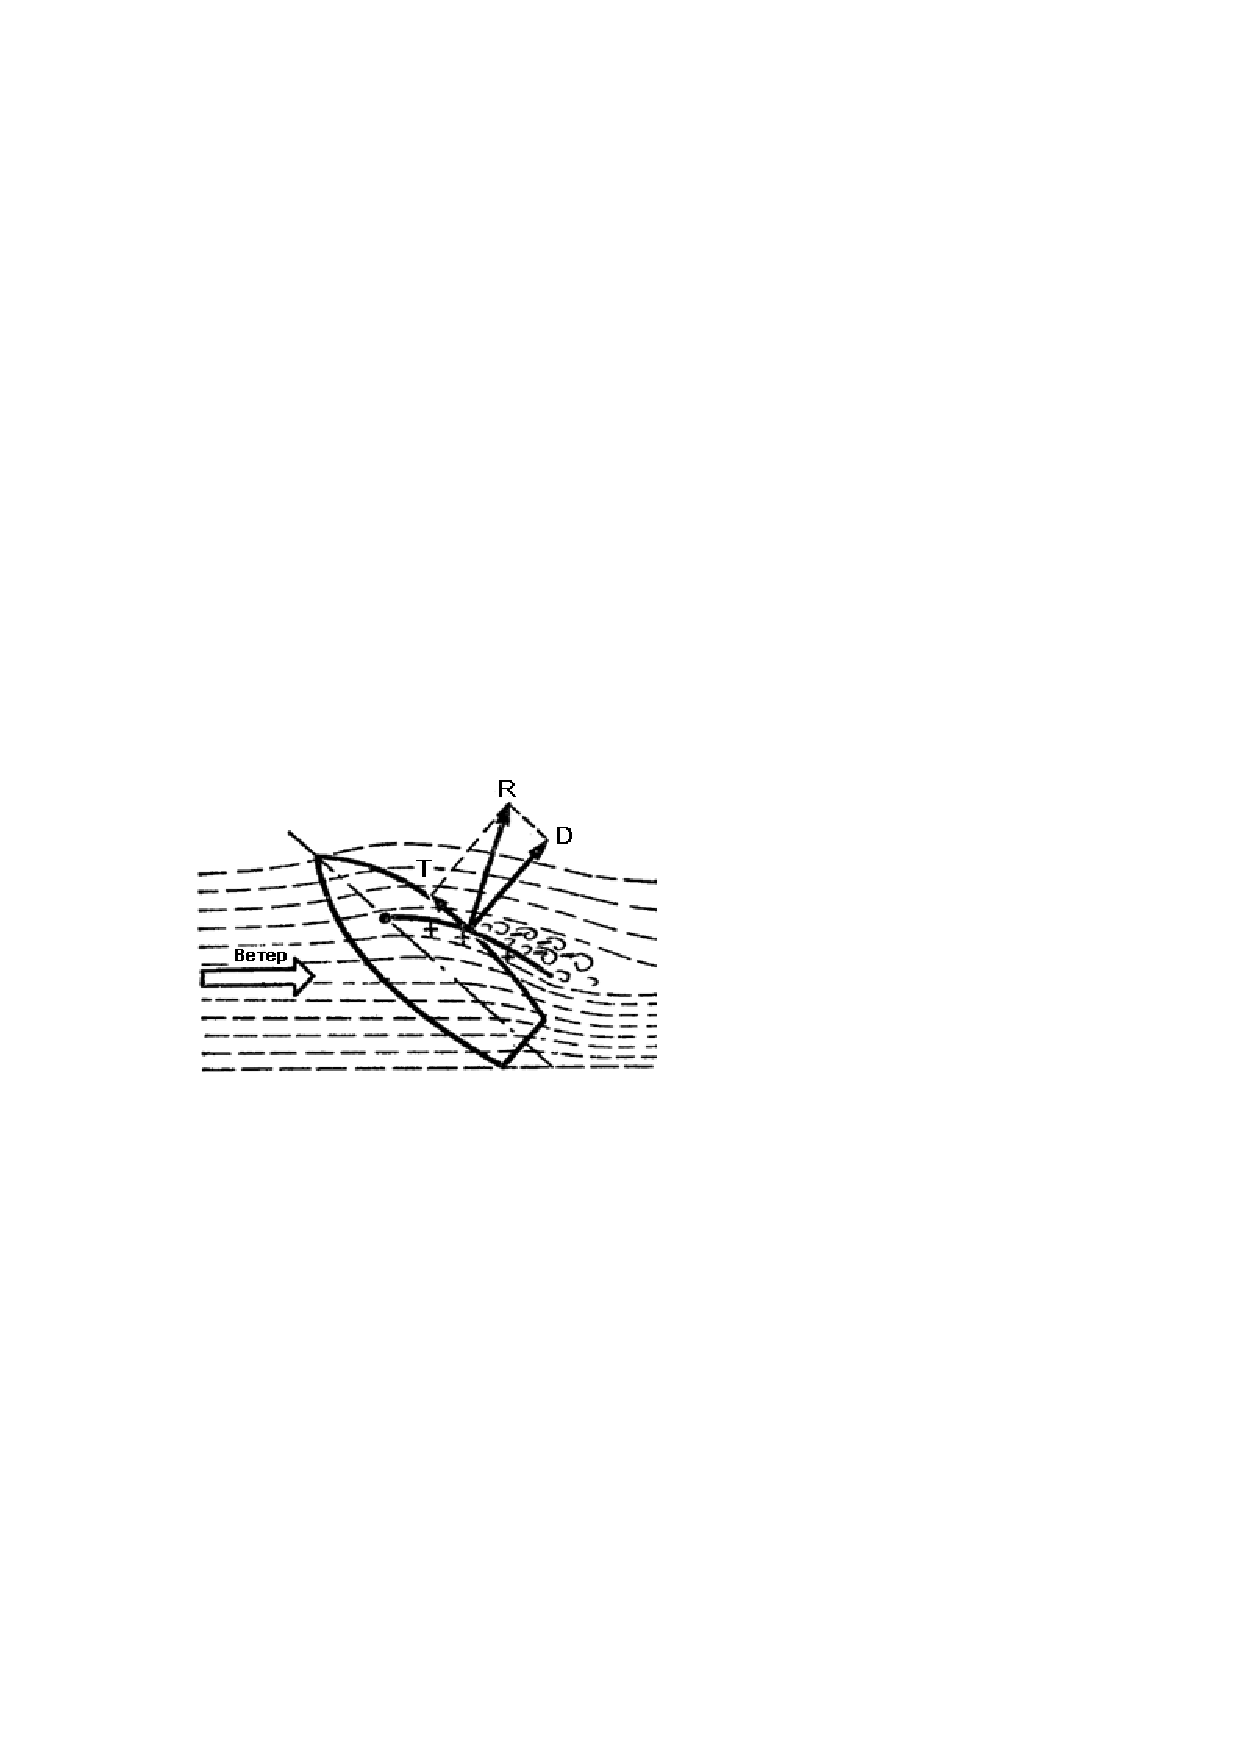
\includegraphics{Deystvie_vetra_ostryy_ugol}
\protect\caption{\label{fig:Deystvie_vetra_ostryy_ugol}Действие
ветра на паруса яхты, идущей под острым углом к ветру}
\end{wrapfigure}%

Как видно на рис.~\ref{fig:Deystvie_vetra_ostryy_ugol},
сила дрейфа имеет значительную величину по сравнению с силой тяги.
Почему же яхта не идет по направлению силы $\overrightarrow{R}$, как это следовало
бы ожидать на первый взгляд?

Сопротивление любого судна в направлении движения много меньше, чем
сопротивление движению в поперечном направлении. Поэтому, несмотря
на то что в данном случае сила тяги меньше силы дрейфа, скорость движения
судна вперед все же больше, чем скорость дрейфа. Однако обычное судно,
например моторный катер, сможет более или менее хорошо ходить под
парусами только с попутными ветрами, когда сила дрейфа сравнительно
невелика по сравнению с силой тяги, так как боковое сопротивление
его недостаточно. Чтобы судно хорошо шло при таком направлении ветра,
как показано на рис.~\ref{fig:Deystvie_vetra_ostryy_ugol},
оно должно иметь достаточно большое боковое сопротивление. У спортивных
парусных судов это достигается с помощью вертикальных плавников, поставленных
под днищем яхты вдоль корпуса.

Кроме того, сила дрейфа вызывает крен яхты, и для противодействия
этому крену всякое парусное судно должно иметь большую \textbf{остойчивость}\index{остойчивость},
то есть способность сопротивляться крену. Особенностью парусного судна
является то, что оно почти всегда идет с креном, достигающим иногда
30\--$40^{\circ}$.

Эти два положения и определяют главное различие между корпусами парусных
яхт \--- различие по способу борьбы с дрейфом и креном.

\begin{figure}[htbp]
\centering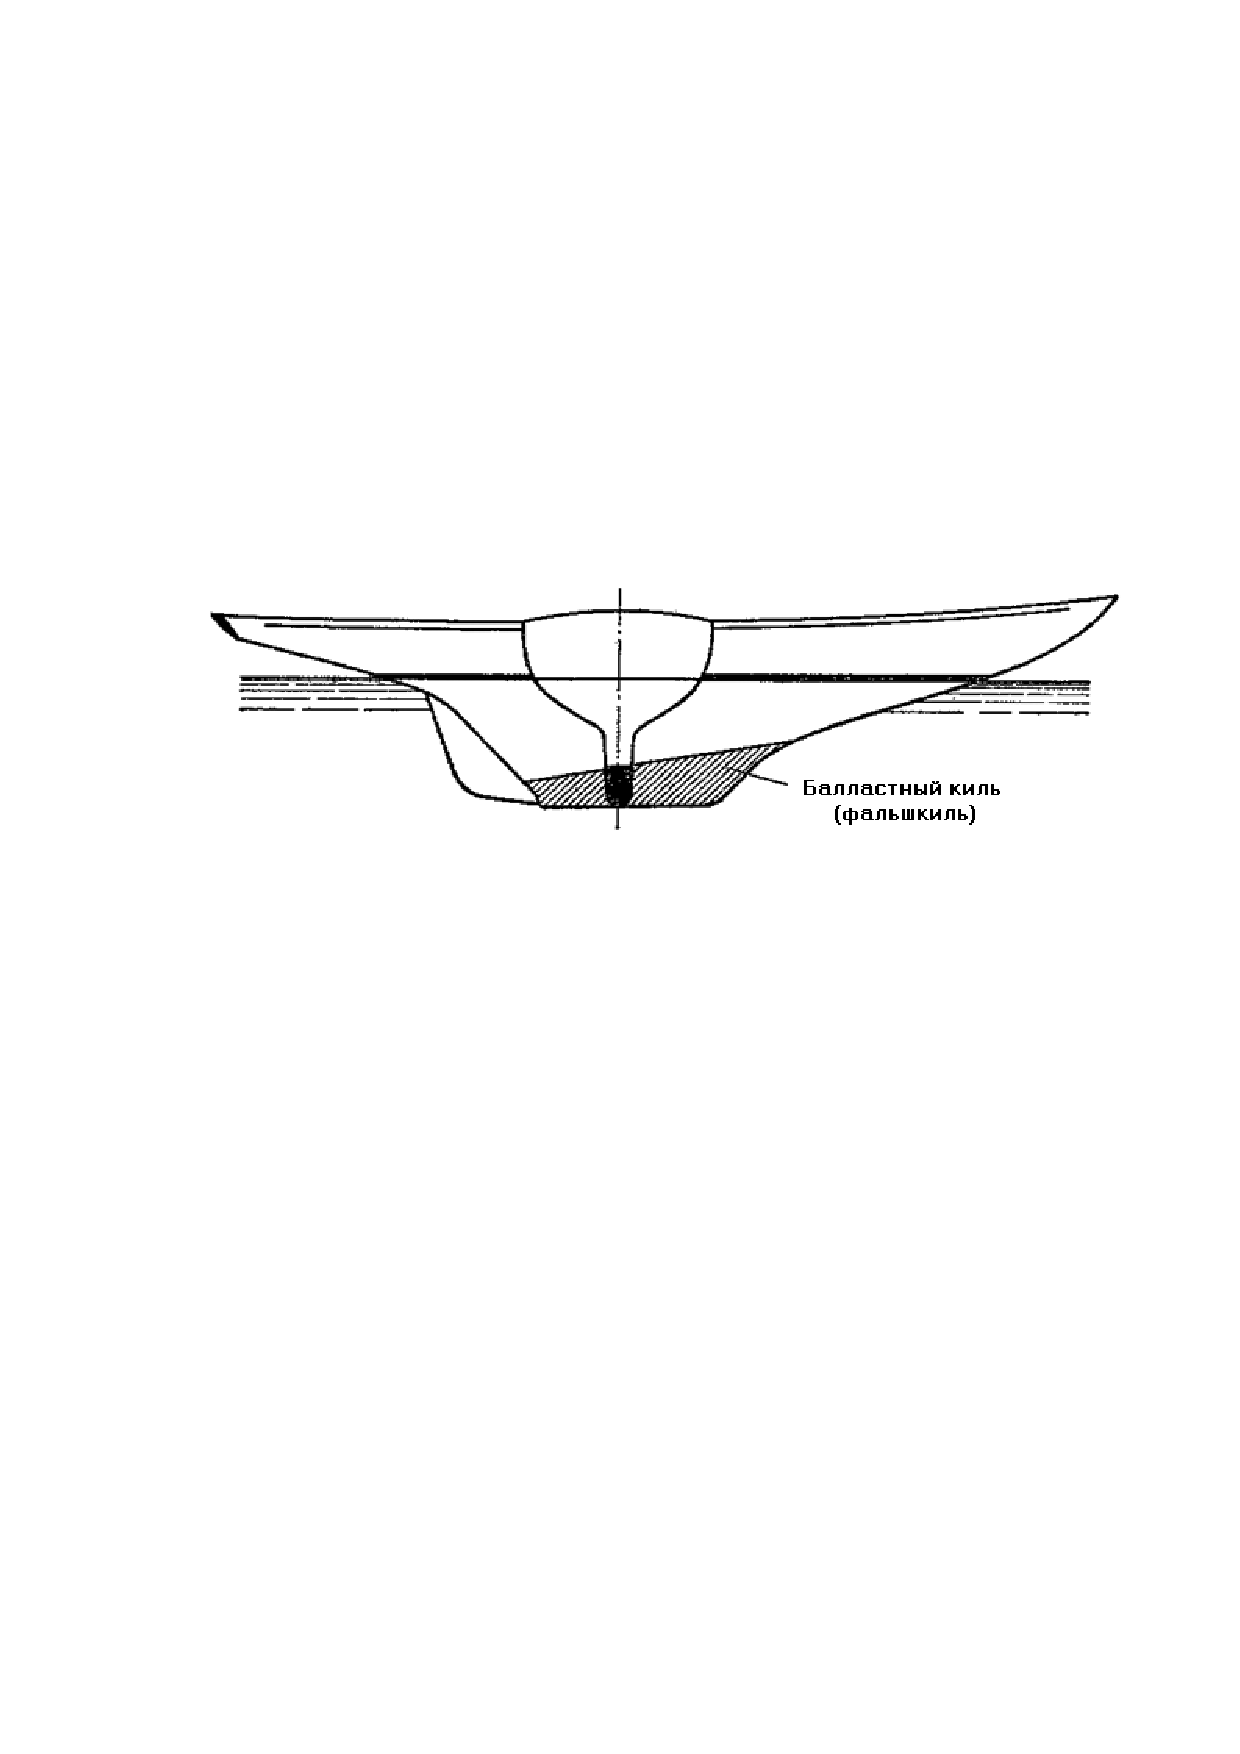
\includegraphics[scale=0.9]{Kilevaya_yachta}
\caption{Килевая яхта}
\label{fig:4}
\end{figure}


Наиболее характерным и распространенным типом парусной яхты является
\textbf{килевая яхта\index{яхта!килевая}}. Форма корпуса
типичной килевой яхты показана на рис.~\ref{fig:4}.
Днище корпуса переходит в глубокий плавник, создающий значительное
боковое сопротивление. Для придания большей остойчивости к нижней
части этого плавника крепится чугунный или свинцовый груз, называемый
\textbf{балластным килем\index{киль балластный}} или
\textbf{фальшкилем}\index{фальшкиль}. Яхты такого типа предназначены
для плавания на морях и озерах с глубокой водой и сильными ветрами
и волнением. Килевая яхта обладает очень большой остойчивостью и в
обычных условиях не может перевернуться. Правда, такая опасность возникает,
когда яхта идет вдоль гребня большой океанской волны (как говорят,
лагом к волне). Так было, например, с яхтой Ф.\,Чичестера во время
его кругосветного плавания. Но даже при таком казусе килевая яхта
все же станет на ровный киль, если имеет хорошую водонепроницаемую
палубу и закрытые люки. Плавать на килевых яхтах по рекам и мелким
озерам затруднительно из-за большой осадки.

\begin{figure}[htbp]
\centering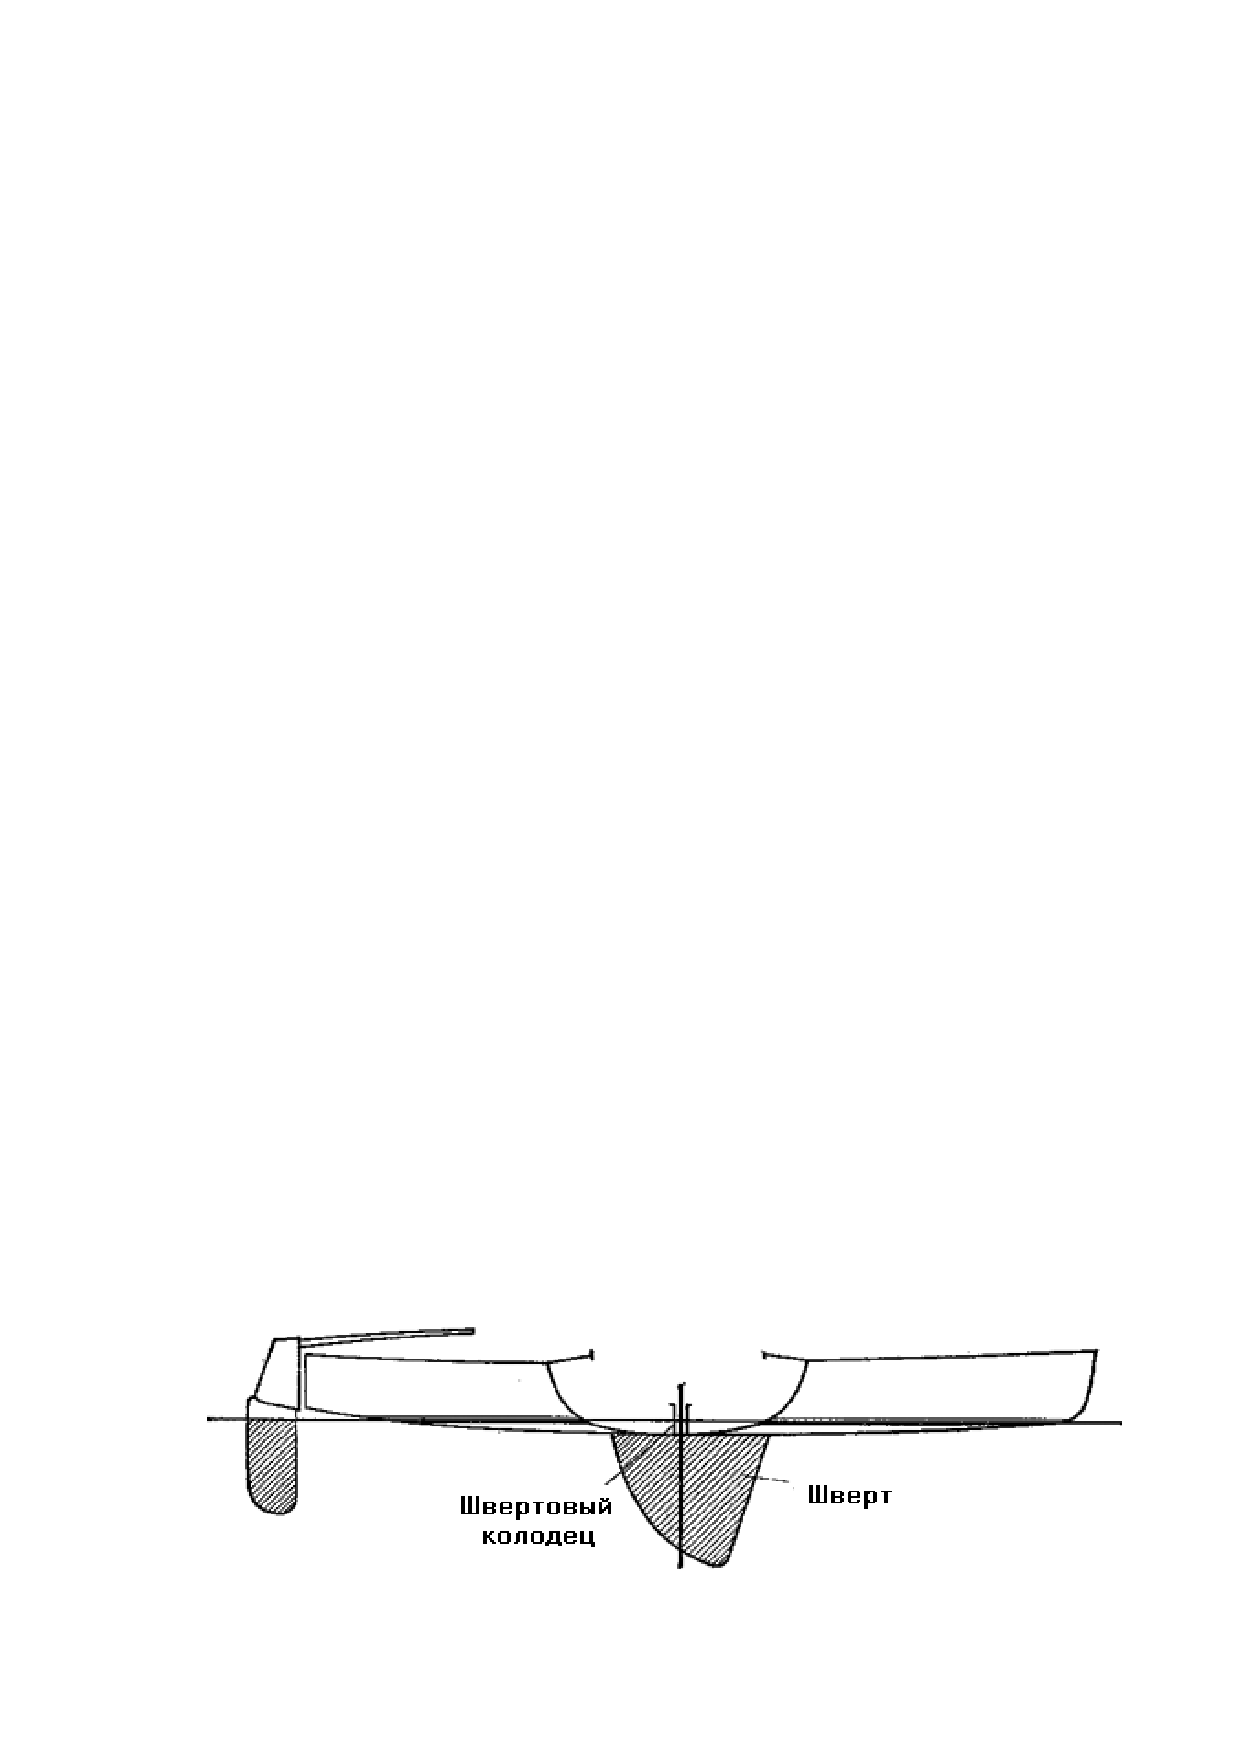
\includegraphics[scale=0.9]{Shvertbot}
\protect\caption{Швертбот}
\label{fig:5}
\end{figure}


\textbf{Швертботы}\index{швертбот} (рис.~\ref{fig:5})
имеют мелкосидящий и относительно широкий корпус. В середине корпуса
сделана щель, в которой помещается плоский (металлический или деревянный)
выдвижной киль \--- \textbf{шверт}\index{шверт}. Щель для прохода
швер-та окружена деревянным или металлическим ящиком \--- \textbf{швертовым
колодцем\index{швертовый колодец}}, верхний срез
которого расположен выше ватерлинии. Когда нет необходимости в дополнительном
боковом сопротивлении (например, при попутных ветрах) или когда проходят
мелкое место, шверт можно поднять и даже совсем убрать в швертовый
колодец.

Остойчивость швертбота много меньше, чем килевой яхты, и обеспечивается
главным образом соответствующей формой корпуса \--- плоского и широкого,
Швертбот может перевернуться при неумелом управлении, поэтому он менее
безопасен при плавании в море и открытых водоемах, чем килевая яхта.
Однако на современных гоночных швертботах с успехом проводят гонки
в тяжелых морских условиях, при штормовых ветрах и большой волне.
И все же крейсерские плавания в открытом море и на крупных озерах
на крейсерских швертботах рискованны и, как правило, не разрешаются.

Существуют еще промежуточные типы яхт, совмещающие характеристики
описанных судов. Так, для получения повышенной остойчивости при небольшой
осадке строят суда, имеющие шверт, проходящий внутри балластного киля
(рис.~\ref{fig:6}).
У этих судов осадка без шверта меньше, чем у килевых яхт, но больше,
чем у швертботов. Такие яхты называют \textbf{компромиссами}\index{компромисс}.

\begin{figure}[htbp]
\centering
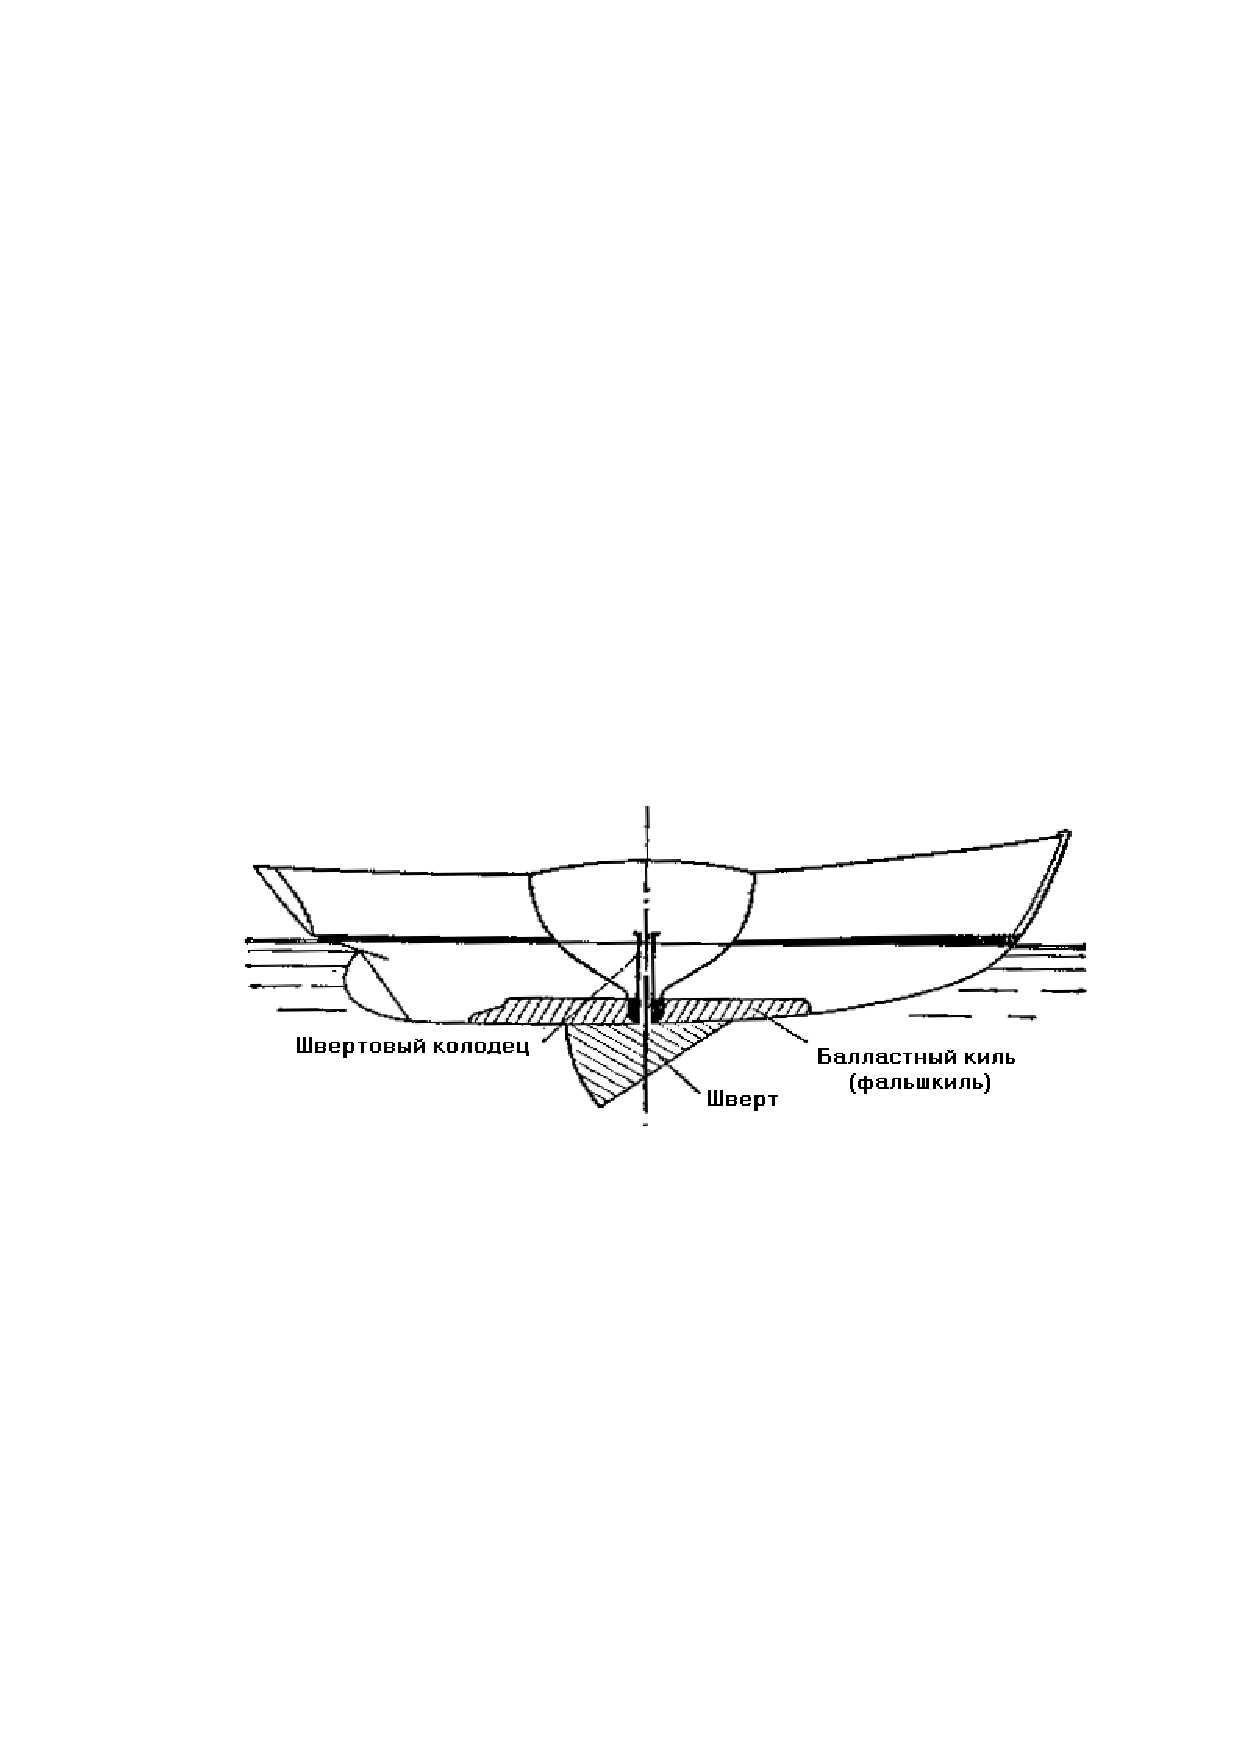
\includegraphics{Kompromiss}
\protect\caption{\label{fig:6}Яхта-компромисс}
\end{figure}


Раньше компромиссы использовались главным образом как крейсерские
яхты в районах, где имеются значительные открытые водные пространства
с сильными ветрами, но с малой водой, а также для комбинированного
плавания, когда приходится часто ходить из реки в море, канал, водохранилище
и т.\,п. Однако в последние годы появилось много крейсерско\-/гоночных
компромиссов для морского и даже океанского плавания, у которых шверт
ставится для регулируемого изменения бокового сопротивления яхты.

\begin{wrapfigure}{O}{0.5\columnwidth}%
\centering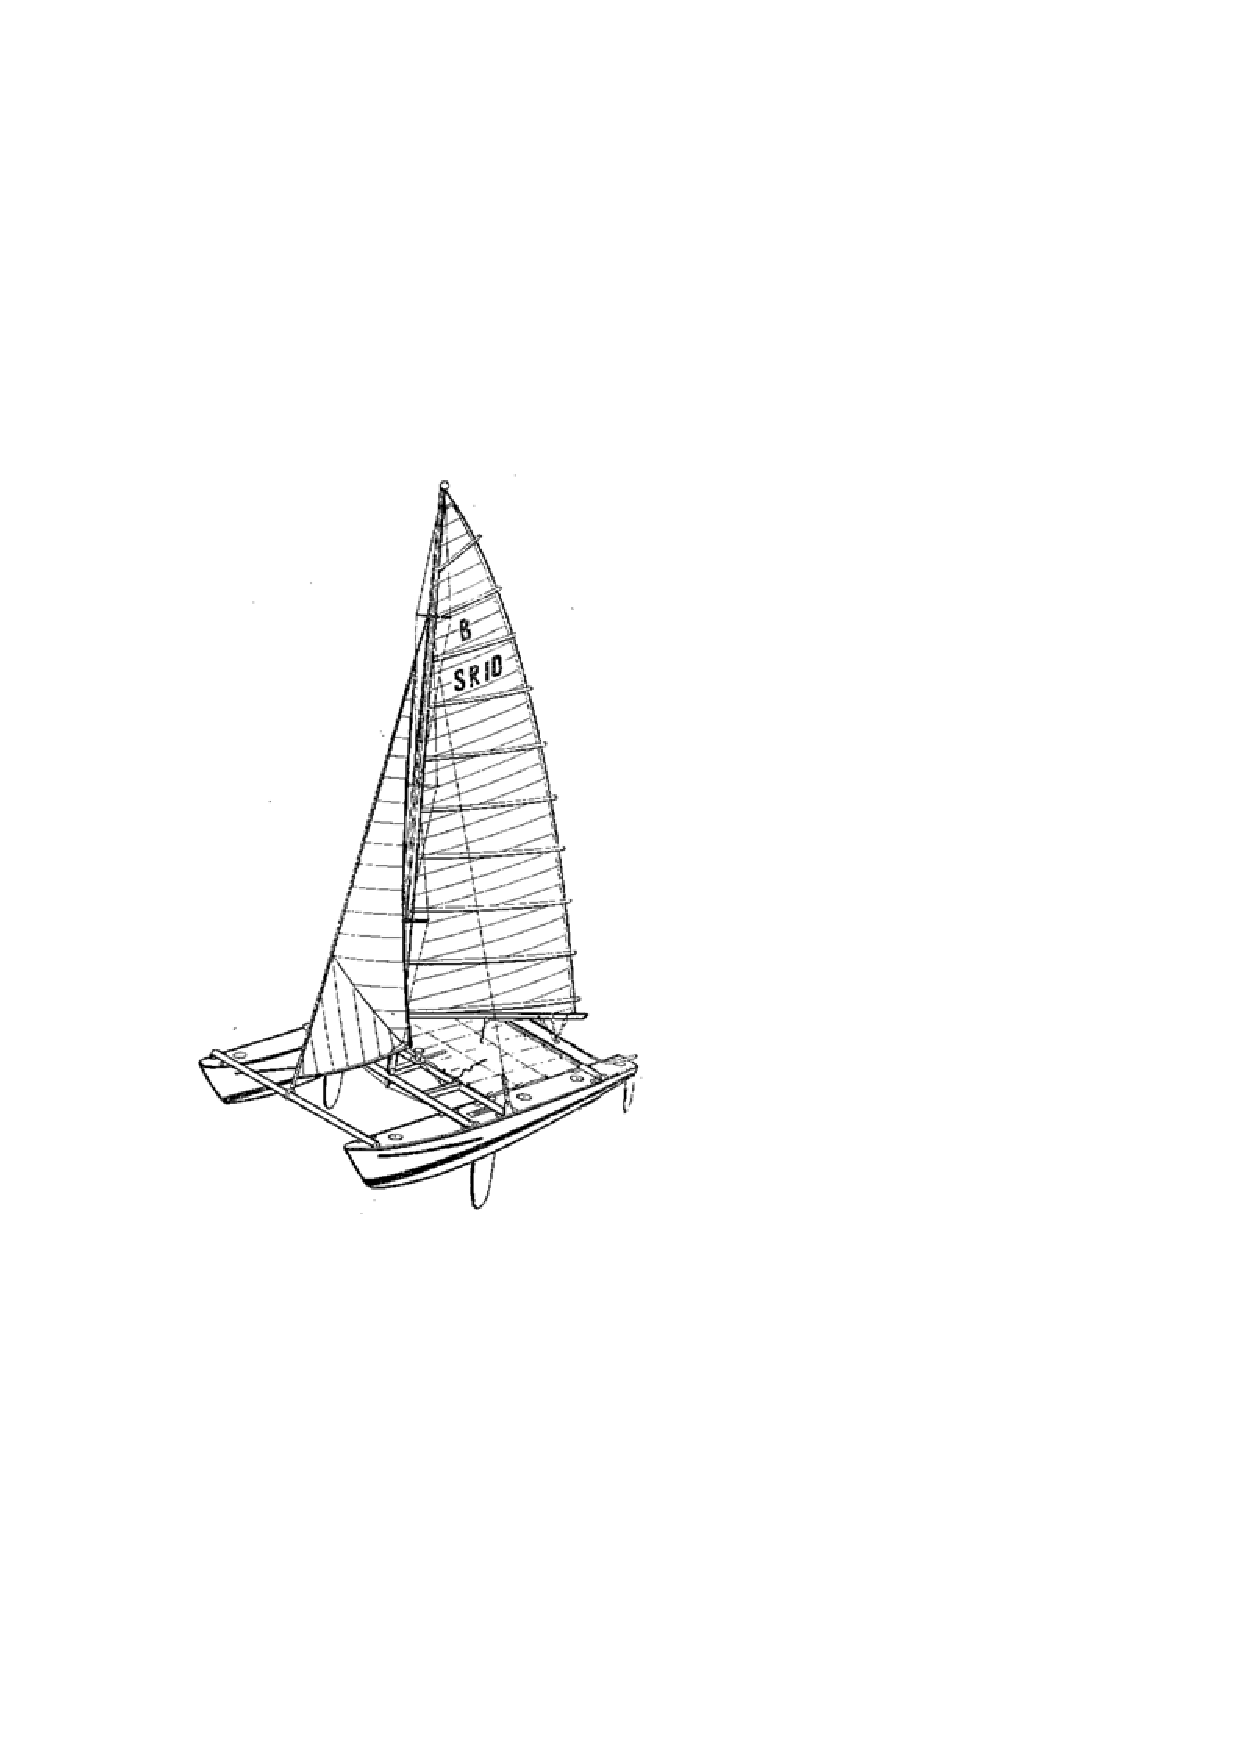
\includegraphics[scale=0.9]{Katamaran_class_B}
\caption{Гоночный катамаран класса <<В>>}
\label{fig:7}
\end{wrapfigure}%


В самые последние годы появились яхты, имеющие вполне <<морскую>>, тяжелую
и прочную, конструкцию, снабженные таким же колодцем, как и швертботы,
с той лишь разницей, что в этом колодце вертикально перемещается тяжелый
профилированный в виде самолетного крыла балластный плавник. Естественно,
что для подъема такого <<шверта>> требуются специальные силовые приводы,
например гидравлические. Подобные яхты по международным правилам обмера
крейсерско-гоночных яхт называются яхтами с <<падающими>> килями.

До сих пор мы говорили о яхтах, имеющих один корпус. Однако существуют
еще и многокорпусные яхты \--- катамараны и тримараны.

\textbf{Катамараны\index{катамаран}} (рис.~\ref{fig:7})
имеют два одинаковых узких длинных корпуса, разнесенных на такое расстояние,
чтобы обеспечить большую остойчивость. Сопротивление таких корпусов
значительно меньше, чем корпуса обычной яхты, поэтому катамаран развивает
значительно большие скорости, чем самые быстроходные гоночные швертботы.
Делают и крейсерские катамараны, на которых успешно совершают океанские
плавания с весьма высокими средними скоростями (10\--15 узлов).

\textbf{Тримараны\index{тримаран}} (рис.~\ref{fig:8})
имеют три корпуса: средний (более широкий, чем у катамаранов, но намного
уже, чем у яхт) и два разнесенных и слегка приподнятых боковых, очень
узких. Боковые корпуса, по существу, являются поплавками, обеспечивающими
остойчивость. При крене тримаран идет на среднем корпусе и одном из
боковых. Тримараны получили в свое время большую популярность как
крейсерские яхты, но сейчас к ним интерес в значительной степени упал.
Дело в том, что на волне они довольно плохо управляемы, имеют резкую
качку и испытывают сильные удары, которые могут привести к разрушениям.
Большая начальная остойчивость на малых углах крена не защищает тримараны
(как, впрочем и катамараны) от стремительного переворачивания, если
ветровые и волновые условия (или ошибки в управлении) приводят к незначительному
превышению допустимых углов крена. И тогда уже катамаран или тримаран
поставить в море <<на ровный киль>> практически невозможно.

\begin{figure}[htbp]
\centering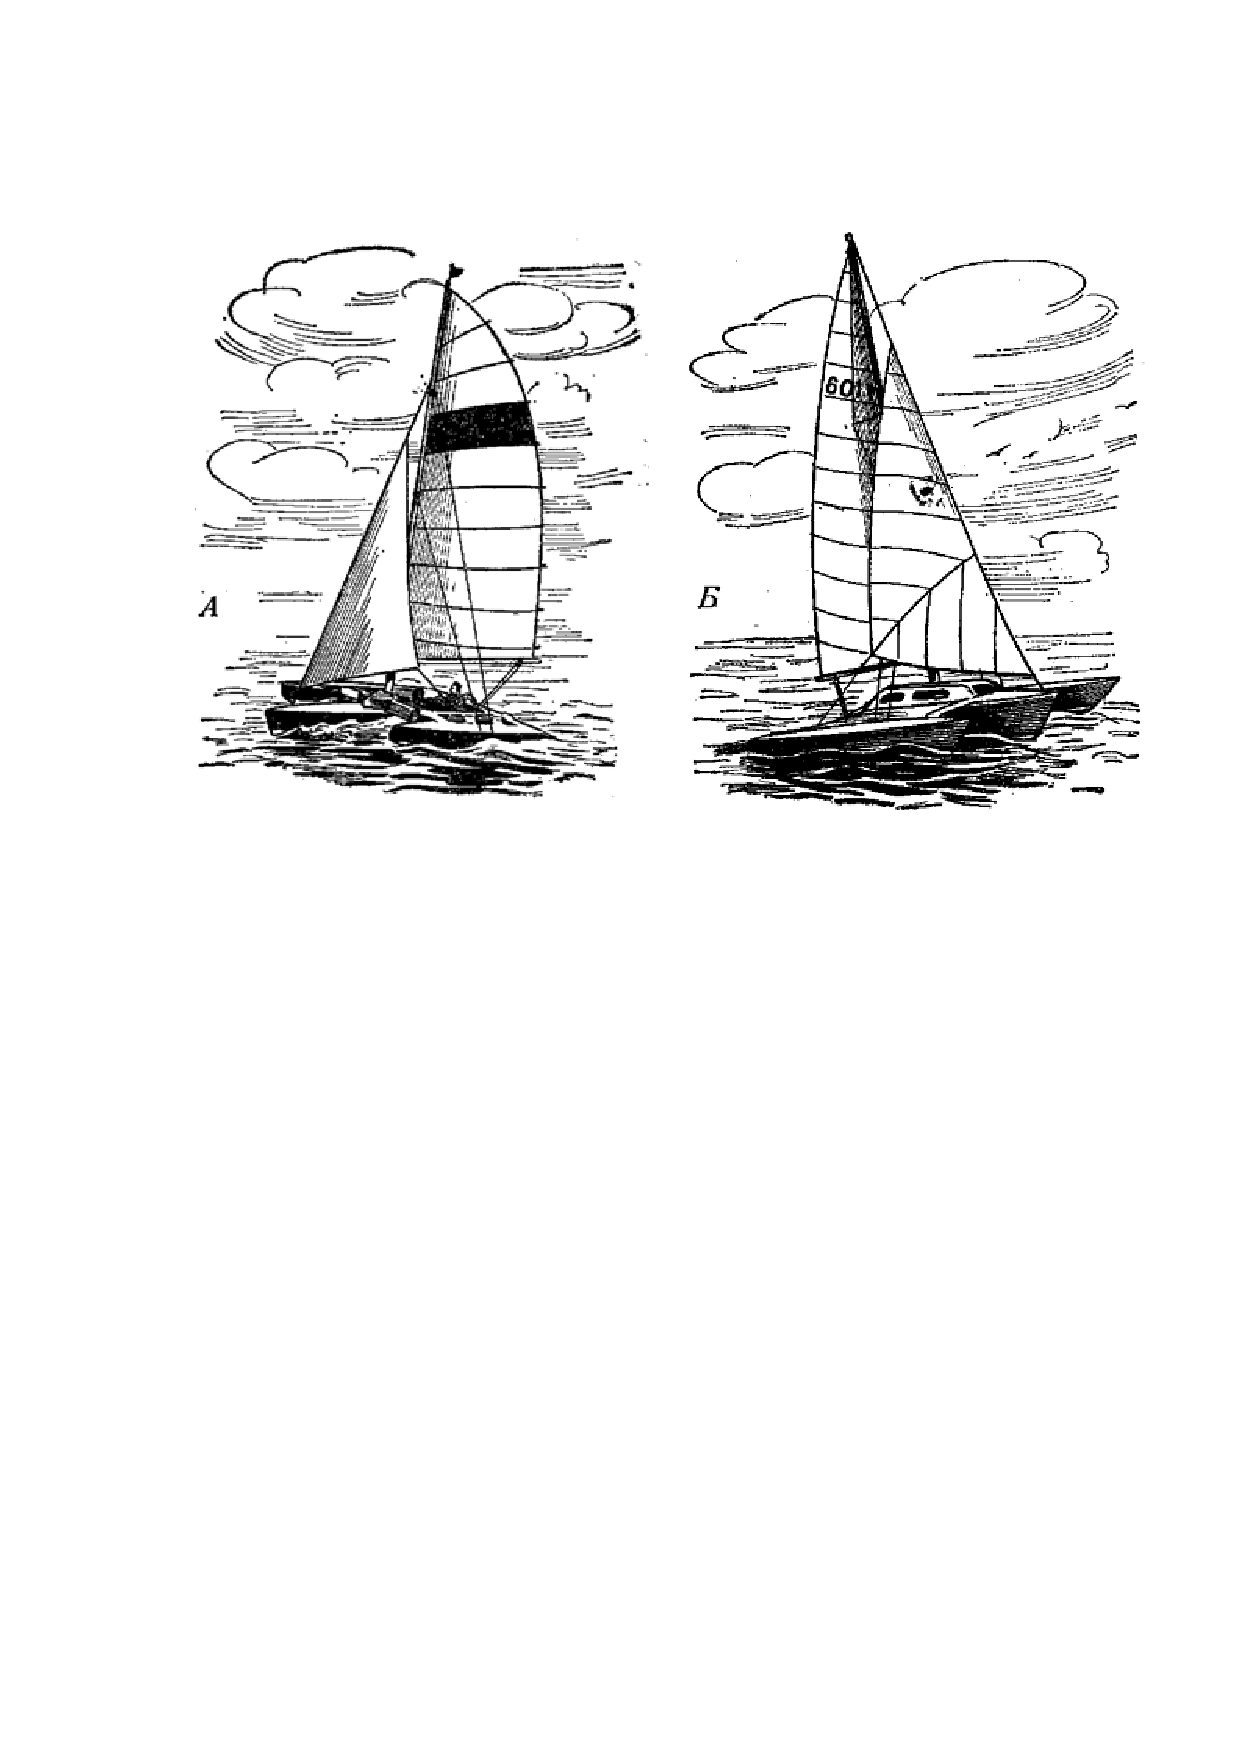
\includegraphics[scale=0.9]{Trimaran}
\caption{\label{fig:8}Тримаран}
\begin{centering}\small
А~---~гоночный, Б~---~крейсерский\par
\end{centering}
\end{figure}


Катамараны успешно развиваются как очень <<спортивные>> гоночные суда.
Однако как крейсерско-гоночные яхты они не оправдали надежд ни в отношении
скорости, ни в отношении безопасности. В серьезных океанских гонках
за многие

годы почти не было крупных аварий яхт, не говоря уже о катастрофах.
А вот случаи аварий и даже гибели катамаранов и тримаранов в открытом
море довольно часты. Так, гонки через Атлантику в 1968\,г. привлекли
сорок три яхты, в составе которых было одиннадцать тримаранов и четыре
катамарана. Из многокорпусных яхт до финиша дошли только четыре, а
в числе призеров был всего один катамаран. Почти все сошедшие с гонки
катамараны и тримараны имели более или менее тяжелые аварии, чудом
обошедшиеся без человеческих жертв.

Все это заставляет относиться к крейсерским многокорпусным яхтам с
известной осторожностью, хотя в трансатлантических гонках 1972\,г.
тримараны выступали значительно лучше, заняв первое, третье и пятое
места в этой грандиозной гонке.

\begin{figure}[htbp]
\centering
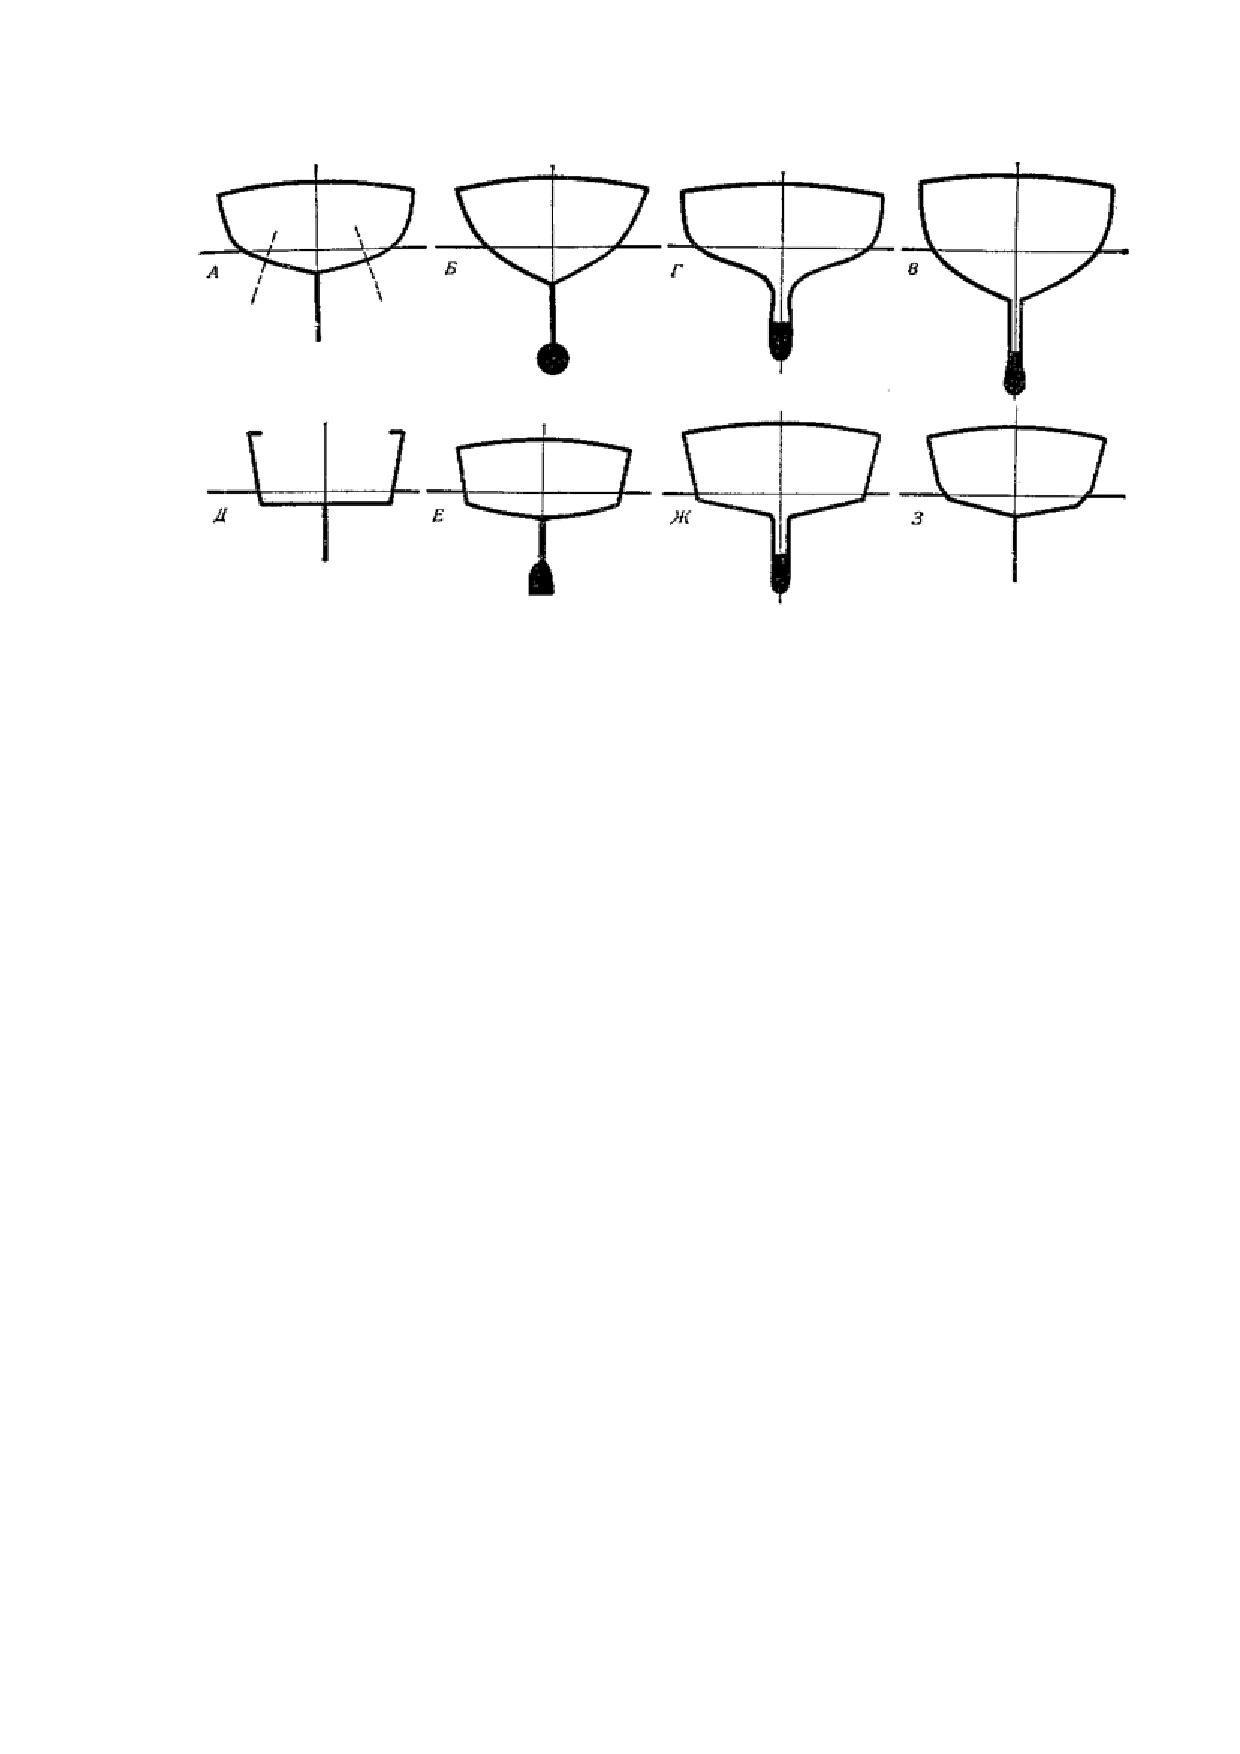
\includegraphics[scale=0.9]{Formy_midel_shpangoutov}
\protect\caption{\label{fig:9}Формы мидель-шпангоутов}

\begin{centering}\small
Круглошпангоутные яхты: А~---~швертбот; Б~---~килевая яхта с бульбкилем
(класс <<Темпест>>); В~---~килевая яхта с плавниковым килем; Г~---~килевая
яхта обычной формы.
\par\end{centering}

\centering{}\small
Яхты-шарпи: Д~---~швертбот (класс <<Оптимист>>); Е~---~килевая
яхта с бульбкилем (<<Звезднын класс); Ж~---~килевая яхта с плавниковым
килем; 3~---~шарпи с подрезанной скулой
\end{figure}


Наружная форма корпуса яхты характеризуется формой её поперечного
сечения, а также видом носа и кормы. При сравнении судов рассматривают
сечение, проходящее примерно через середину яхты. Называется оно сечением
по мидель-шпангоуту или миделем. 

По форме миделя все яхты независимо от типа подразделяют на яхты с
округлым миделем, или круглошвангоутные (рис.~\ref{fig:9},
\emph{а, б, в} и \emph{г}), и с угловатым миделем, или шарпи (рис.~\ref{fig:9},
\emph{д, е, ж} и \emph{з}), форма которого составлена из прямых или
кривых линий, образующих углы.

Постройка яхт с угловатыми шпангоутами проще и обходится несколько
дешевле, но эти яхты немного проигрывают круглошпангоутным во внешнем
виде и скорости хода. Поэтому гоночные яхты чаще всего строятся круглошпан-гоутными,
хотя есть немало яхт с угловатым миделем, завоевавших большую популярность
(юношеские классы <<Кадет>>, <<Оптимист>>, яхта <<Звездного класса>> и многие
другие).

Классическая форма миделя килевой яхты округлая,с плавным, как говорят
<<зализанным>>, переходом от днища к плавнику. Такую форму имеет большинство
более или менее крупных килевых яхт, и гоночных, и крейсерских.

Иногда переход от днища к фальшкилю бывает не плавный (рис.~\ref{fig:9},
\emph{в} и \emph{ж}), а резкий, и фальшкиль крепится на деревянном
плавнике. Яхты с такой формой миделя называются яхтами с плавниковым
килем. Сейчас широко распространены яхты с так называемым бульб-килем\index{бульб-киль} \--- вертикальным профилированным тонким плавником с сигарообразным балластом
(бульбом) снизу. Такие кили имеют яхты олимпийских классов.

\begin{figure}[htbp]
	\begin{minipage}[b]{0.49\textwidth}
		\centering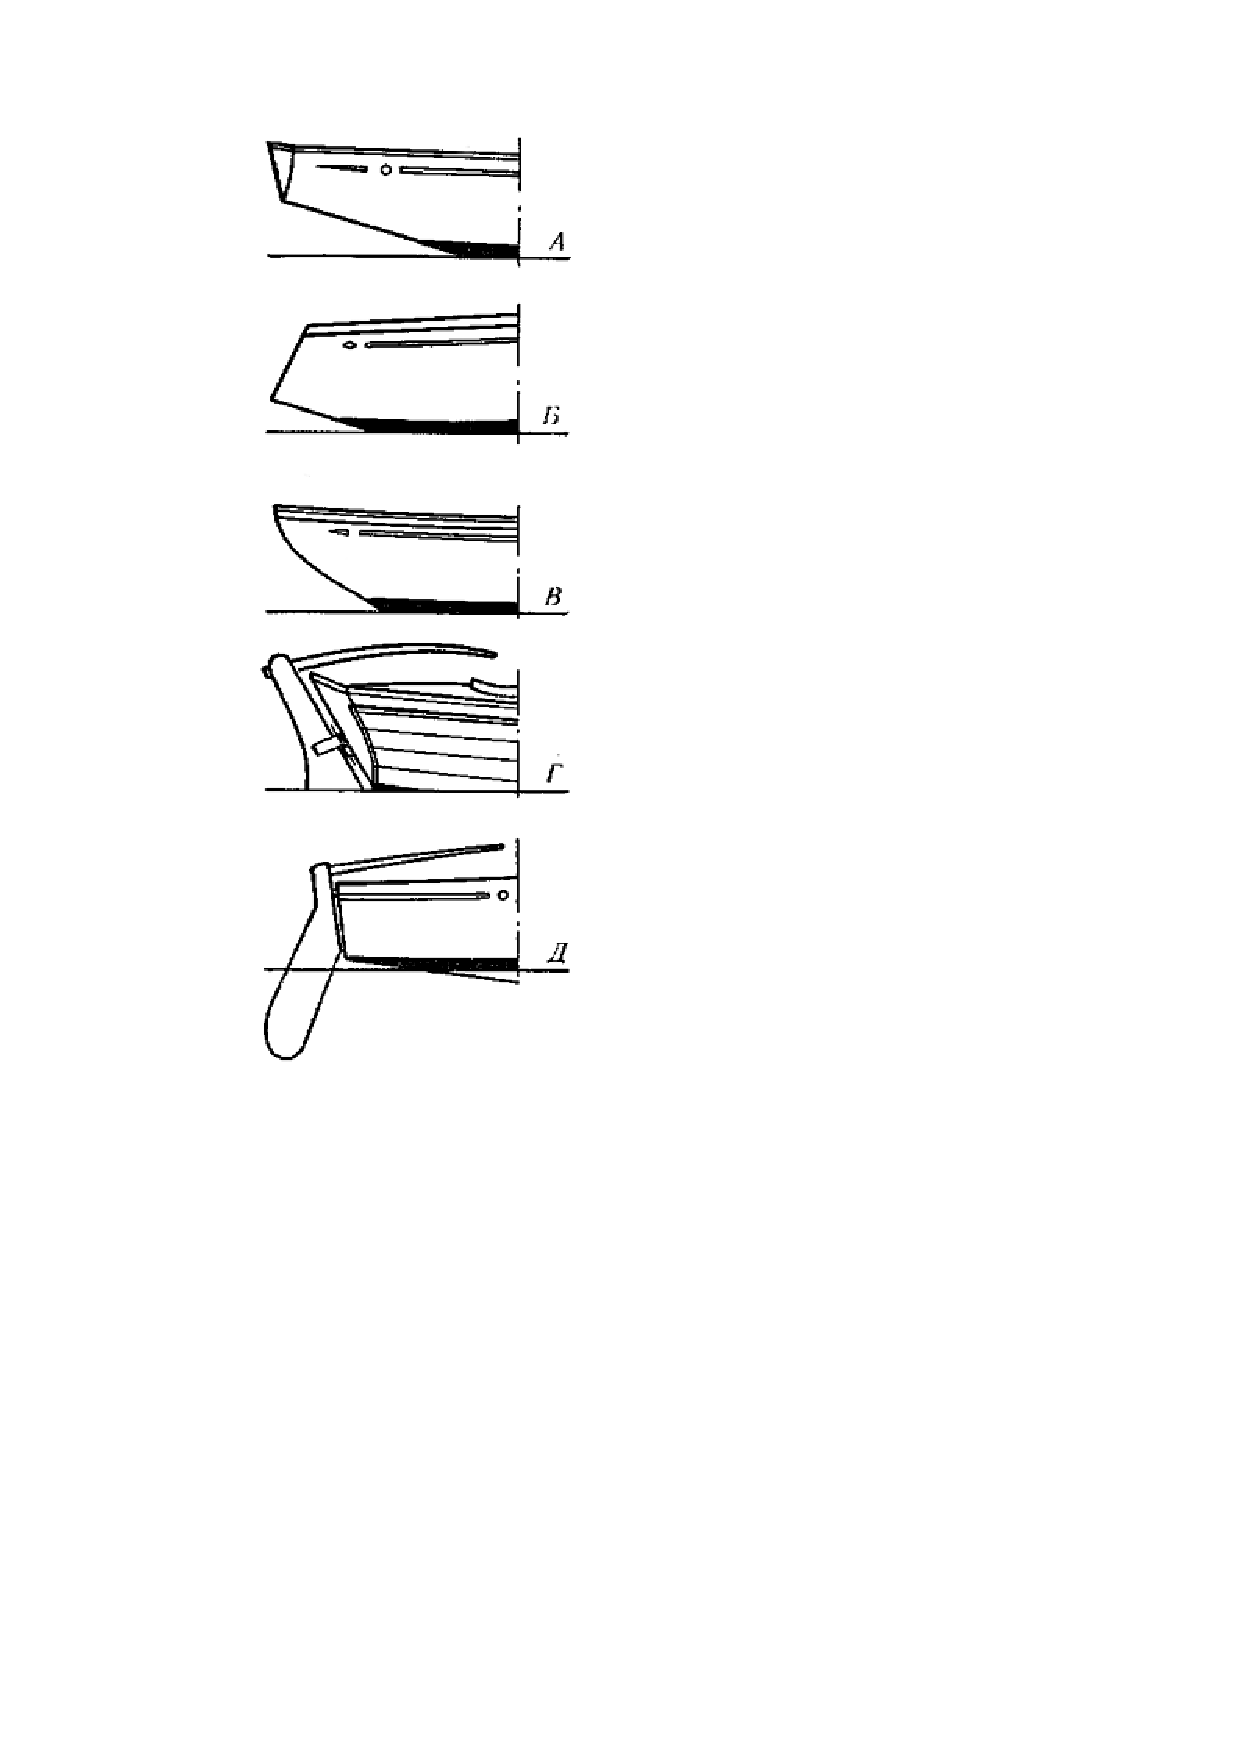
\includegraphics{Formy_korma}
		\caption{Формы кормовых частей}
		\label{fig:10}
	\end{minipage}
	\hfil\hfil%
	\begin{minipage}[b]{0.49\textwidth}
		\centering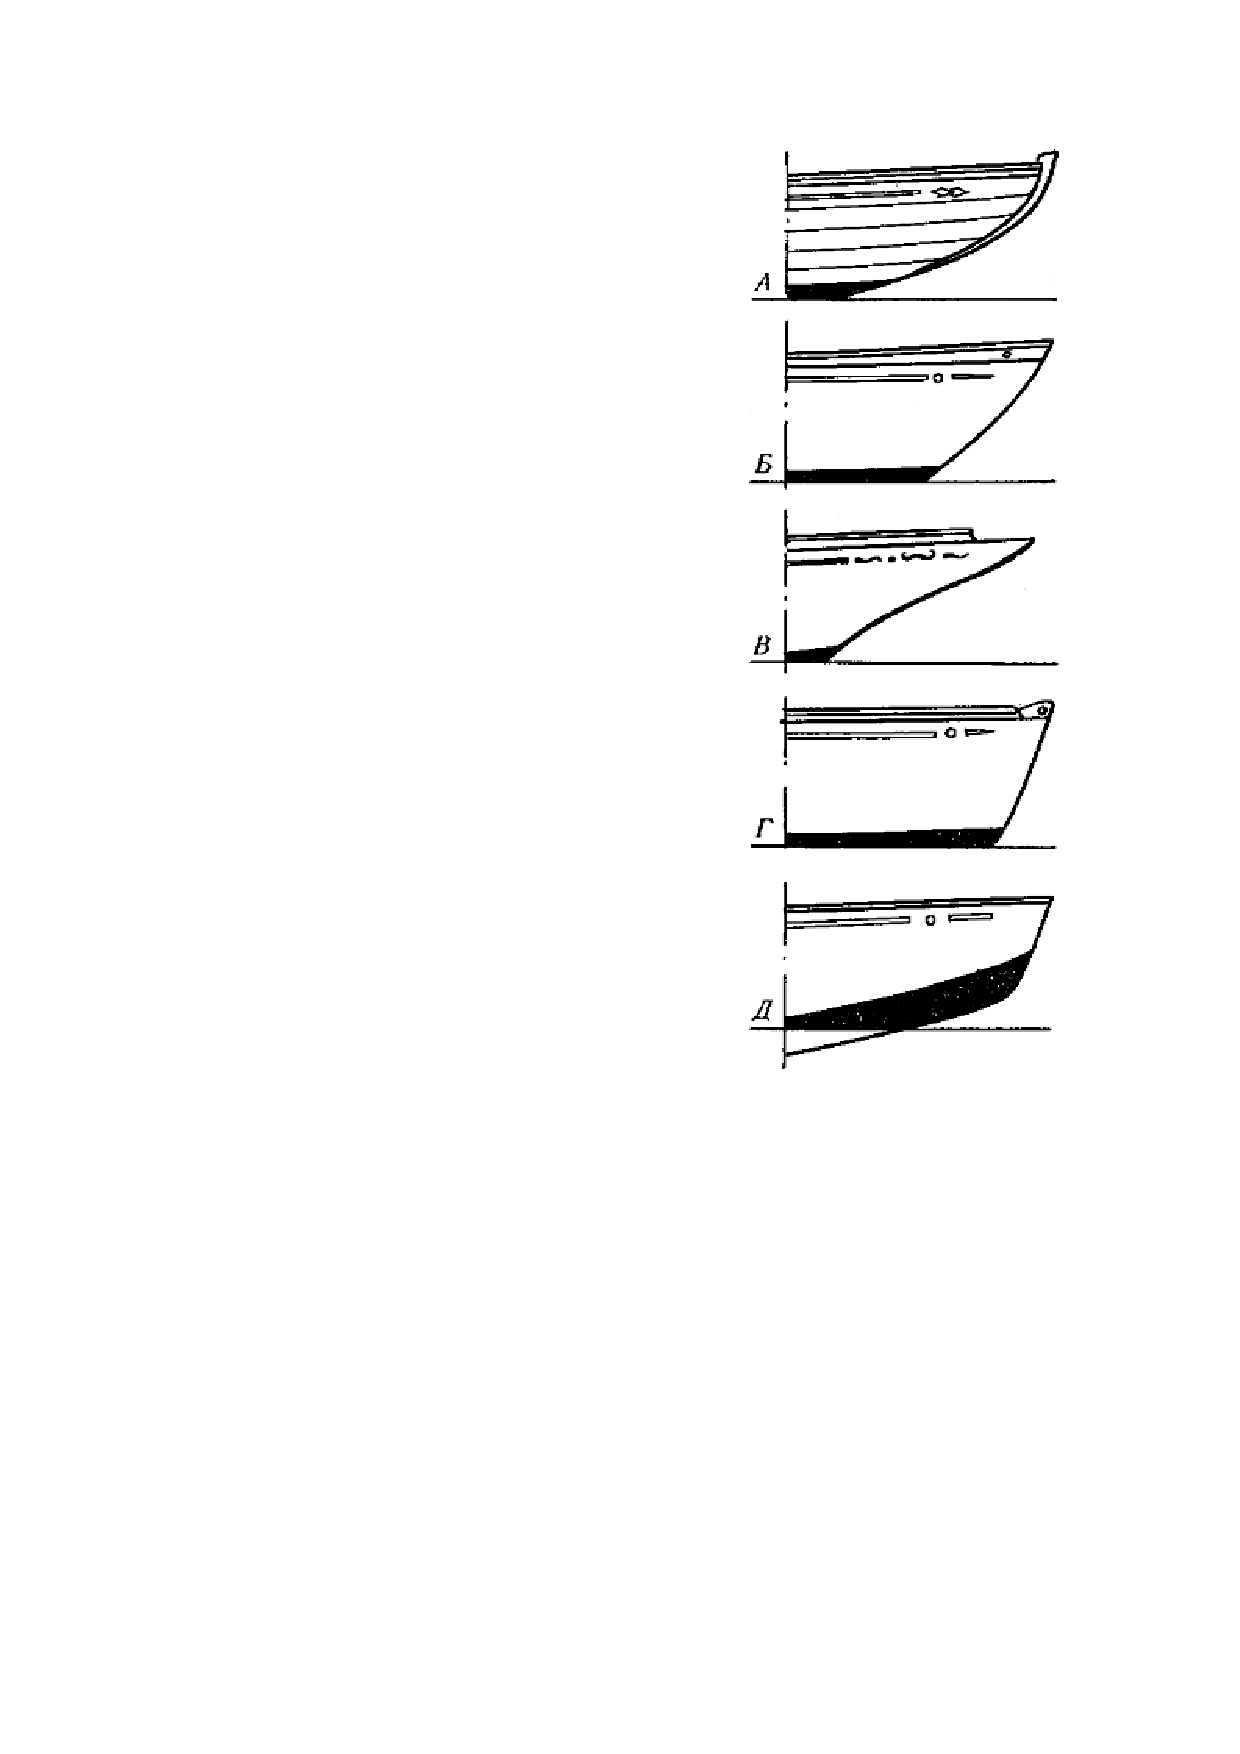
\includegraphics{Formy_nos}
		\caption{Формы носовых частей}
		\label{fig:11}
	\end{minipage}
	\par
	\smallskip
	\begin{minipage}[b]{0.49\textwidth}
		\centering\small
		А~---~яхтенная корма с нормальным транцем;
		Б~---~то же с реверсивным транцем;
		В~---~байдарочная корма;
		Г~---~транцевая обрезнаякорма килевой яхты;
		Д~---~то же швертбота
	\end{minipage}
	\hfil\hfil%
	\begin{minipage}[b]{0.49\textwidth}
		\centering\small
		А~---~ложкообразный штевень;
		Б~---~современный наклонныв штевень;
		В~---~клипер-штевень;
		Г~---~прямой штевень;
		Д~---~транце выйнос (форшпигель) швертбота <<Кадет>>
	\end{minipage}
\end{figure}

<<Звездный>> и <<Темпест>>, а также множество крейсерско\-/гоночных яхт
малого размера. Швертботы, как и килевые яхты, делают и с угловатым
миделем (рис.~\ref{fig:9}, \emph{д}), и с округлым (рис.~\ref{fig:9},
\emph{а}). Кроме того, различают швертботы с одним и двумя швертами.

У одношвертовика шверт расположен в диаметральной плоскости судна.
У двухшвертовика оба шверта поставлены под углом (пунктиры на рис.~\ref{fig:9}, \emph{а}), поэтому он несколько лучше сопротивляется дрейфу при больших
углах крена. При сильном крене один из швертов не работает, а часто
и совсем выходит из воды; второй шверт в это время оказывается почти
в вертикальном положении, тогда он принимает всю работу по противодействию
дрейфу на себя.

В настоящее время двухшвертовики применяются очень редко.

По форме носа яхты традиционно делятся на прямоштевники, яхты с ложко-образным
штевнем и клипперштевнем (рис.~\ref{fig:11}).
Однако сейчас ложкообразные штевни с большим носовым свесом вышли
из моды, и большая часть современных яхт и швертботов имеют носы типа,
изображенного на рис.~\ref{fig:11},
\emph{б}. Прямой штевень в чистом виде сохранился сейчас только у
некоторых швертботов. Давно исчезнувшие клипперштевни (рис.~\ref{fig:11},
\emph{в}) в наши дни все чаще и чаще появляются не только на крупных
моторных и парусно-моторных яхтах, но и на небольших крейсерах.

У мелких швертботов и яхтенных шлюпок (тузиков) нос часто заканчивается
не острым форштевнем, а плоским наклонным срезом (рис.~\ref{fig:10},
\emph{д}). Такой нос называют транцевым (иногда \--- прам), а сам срез \--- носовым
транцем или форшпигелем. Транцевые носы имеют швертботы юношеских
классов <<Оптимист>> и <<Кадет>>.

По форме кормовой части яхты могут иметь яхтенную корму с нормальными
или обратным (реверсивным) транцем (рис.~\ref{fig:10},
\emph{а, б}), байдарочную (рис.~\ref{fig:10},
\emph{в}) или транцевую обрезную корму. Последняя имеет две разновидности;
одна из них характерна для килевых яхт (рис.~\ref{fig:10},
\emph{г}), другая \--- для швертботов (рис.~\ref{fig:10},
\emph{д}).

%--------------------------------------------------------------------------
%
%                      Различия яхт по типу вооружения
%
%--------------------------------------------------------------------------

\section{Различия яхт по типу вооружения}

\begin{figure}[htbp]
	\begin{minipage}[b]{0.49\textwidth}
		\centering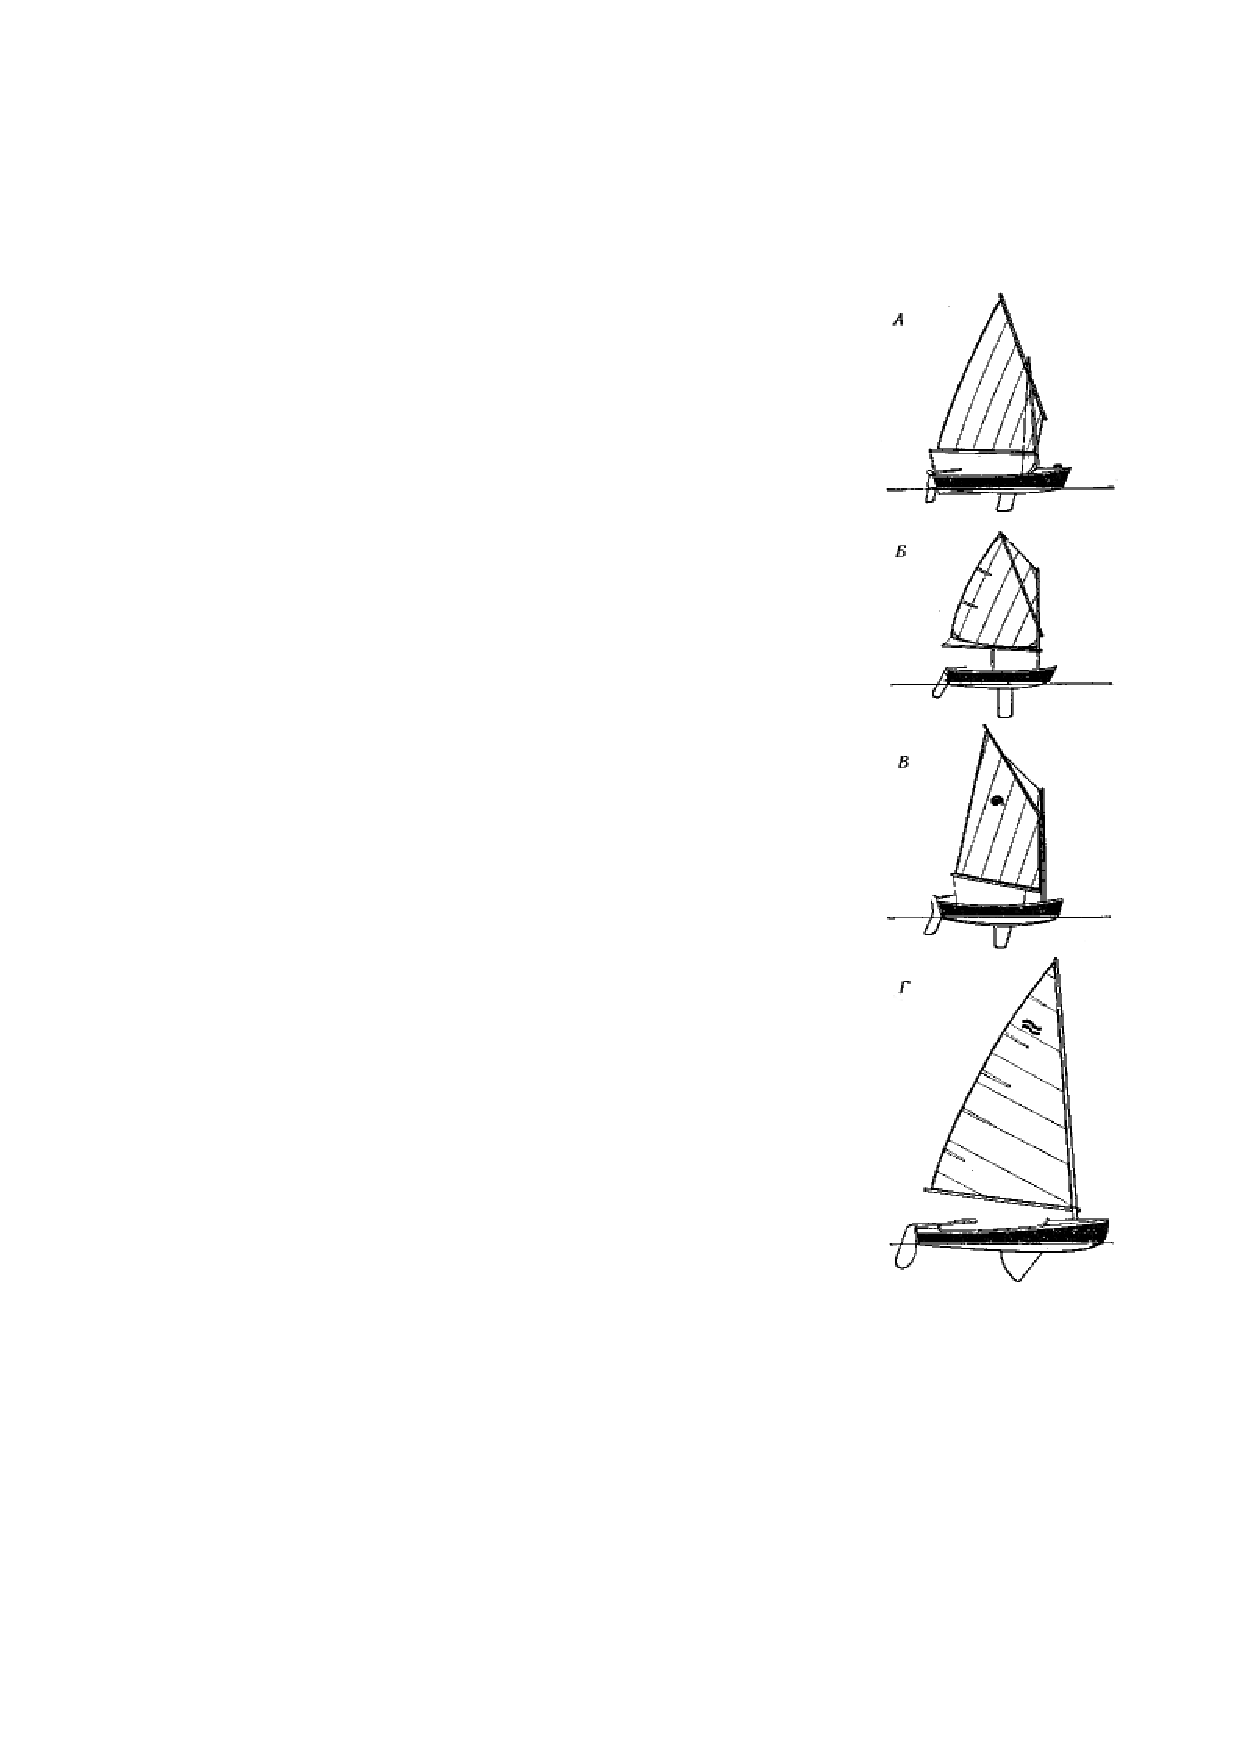
\includegraphics{Kety}
		\caption{Кэты}
		\label{fig:12}
	\end{minipage}
	\hfil\hfil%
	\begin{minipage}[b]{0.49\textwidth}
		\centering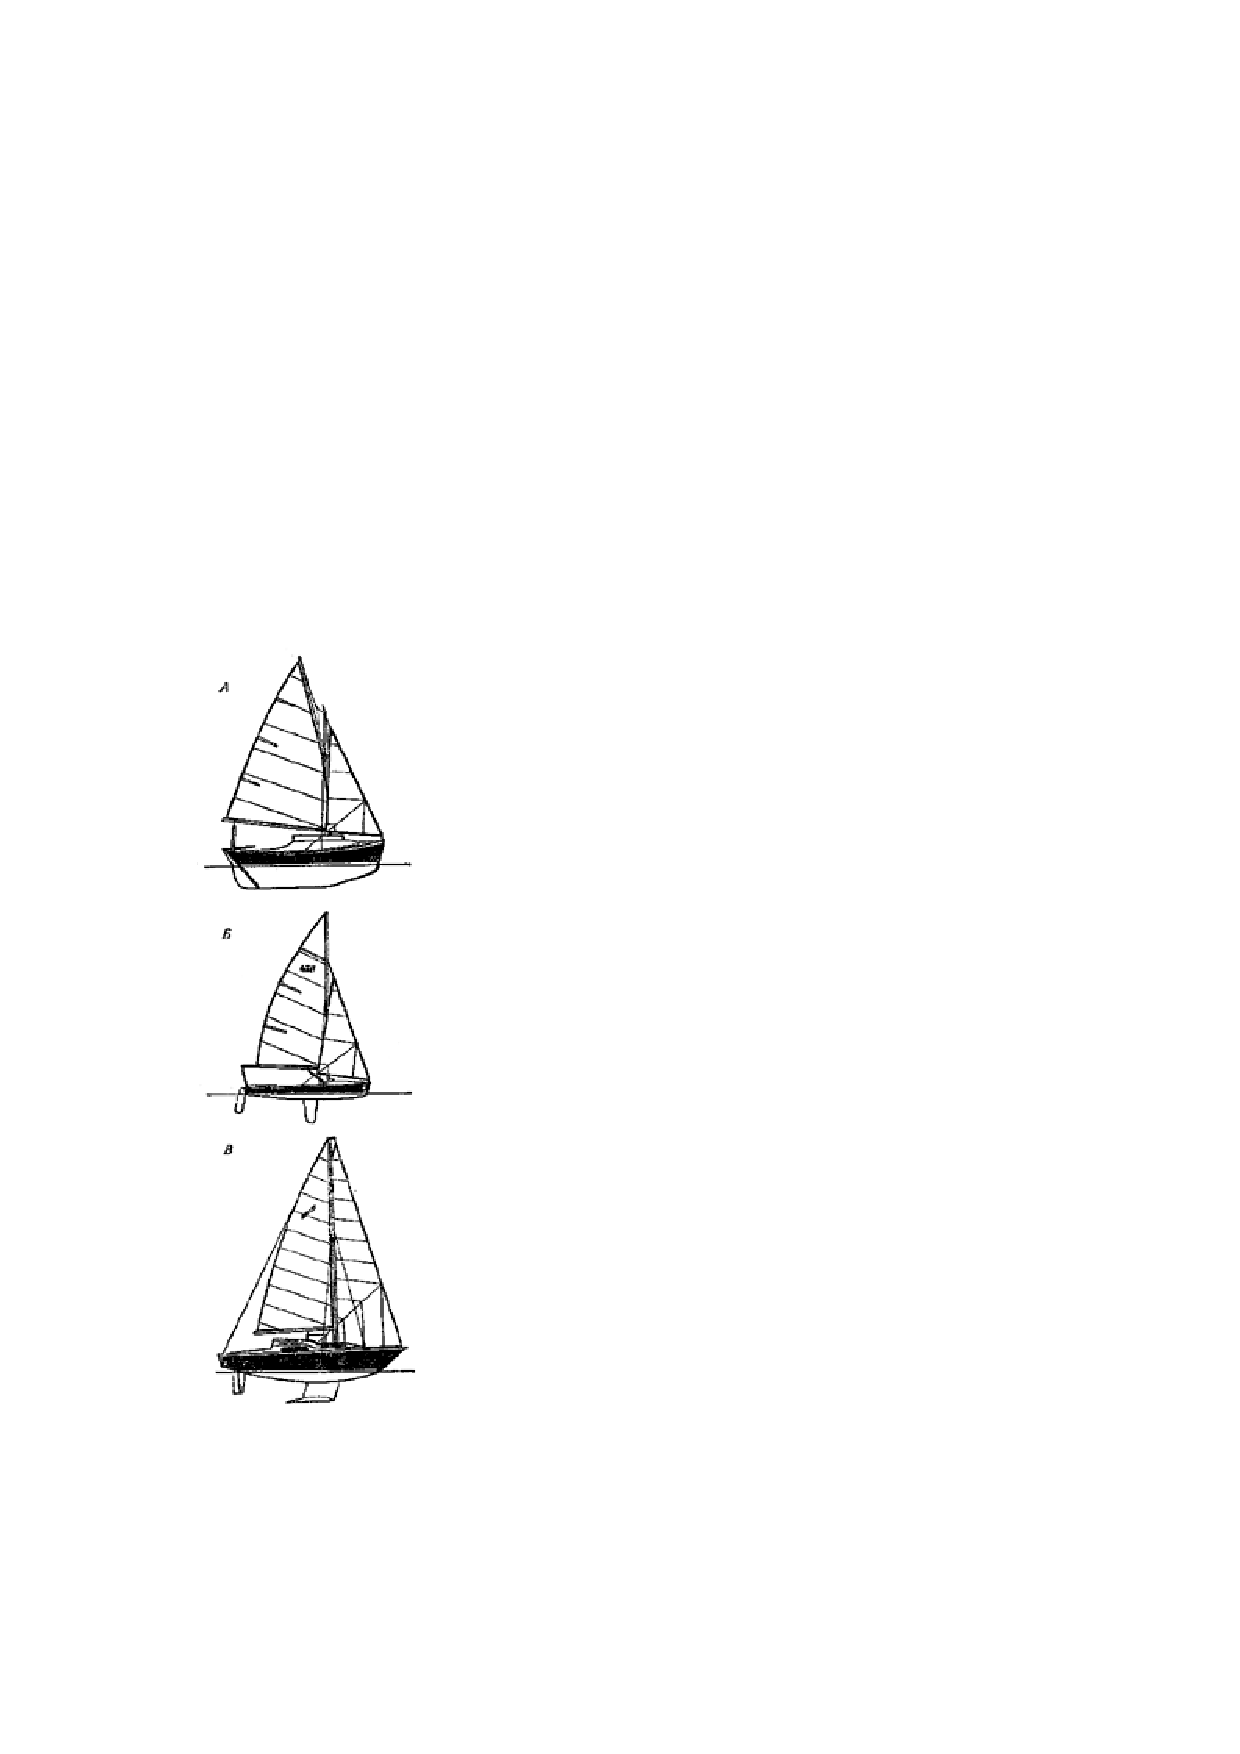
\includegraphics{Shlyupy}
		\caption{Шлюпы}
		\label{fig:13}
	\end{minipage}
	\par
	\smallskip
	\begin{minipage}[b]{0.49\textwidth}
		\centering\small
		А \--- рейковый,
		Б \--- шпринтовый (<<Оптимист>>);
		В \--- гафельный;
		Г \--- бермудский (класс <<Финн>>)
	\end{minipage}
	\hfil\hfil%
	\begin{minipage}[b]{0.49\textwidth}
		\centering\small
		А \--- гафельный;
		Б \--- бермудский обычный (класс <<470>>);
		В \--- бермудский с топовым стакселем
	\end{minipage}
\end{figure}


Типы парусного вооружения довольно разнообразны и зависят в основном
от условий, в которых предстоит плавать судну, и от его размеров.
Вооружение парусных судов различается главным образом по форме основных
парусов.

Большие парусные суда носили (да и сейчас носят) так называемые \textbf{прямые
паруса}\index{паруса!прямые}. Они имеют форму трапеции и поднимаются на горизонтальных
реях, располагаясь симметрично мачте и перед ней. Под такими парусами
судно идет хорошо только с попутным ветром; к ветру оно может идти
только под большим углом \--- порядка 60-70 . На спортивных яхтах прямые
паруса не применяются в качестве основных, но на крупных крейсерах
иногда на попутных курсах ставят прямой дополнительный парус, называемый
\textbf{брифоком}\index{брифок}.

Спортивные парусные яхты вооружают исключительно \textbf{косыми парусами}\index{паруса!косые},
которые располагаются по одну (заднюю) сторону мачты и передней кромкой
крепятся к ней. Косые паруса обеспечивают значительно лучше тяговые
характеристики при плавании против ветра, чем прямые паруса.

Различают несколько видов косых парусов.

Четырехугольный \textbf{гафельный парус}\index{паруса!гафельные} (рис.~\ref{fig:12},
\emph{в} и \ref{fig:13}, \emph{а})
имеет \textbf{гафель}\index{гафель} \--- наклонное рангоутное дерево, одним концом
упирающееся в мачту. К гафелю крепится верхняя шкаторина (кромка)
паруса. Передняя шкаторина паруса крепится к мачте, а нижняя \--- к \textbf{гику}\index{гик},
горизонтальному рангоутному дереву, которое при помощи вертлюга (шарнира) соединено с мачтой. Разновидностью гафельного паруса является парус
\textbf{гуари}\index{паруса!гуари} с очень длинным гафелем (часто длиннее гика и даже
мачты), стоящим почти вертикально.

На маленьких яхтах, преимущественно на открытых парусных тузиках\-/динги,
иногда ставят \textbf{рейковые}\textit{паруса!рейковые} или \textbf{шпринтовые}\index{паруса!шпринтовые} паруса. У
них гафель заменяется рейком, к которому привязывается верхняя шкаторина
паруса, а его передний конец свободно выходит вперед за мачту (рис.~\ref{fig:12}, \emph{а}), или \textbf{шпринтов}\index{шпринтов}
- шестом, который растягивает парус, упираясь нижним концом в мачту,
а верхним \--- в угол паруса по диагонали, как на детском швертботе <<Оптимист>>
(рис.~\ref{fig:12}, \emph{б}).

Бермудский парус (рис.~\ref{fig:12},
\emph{г}) не имеет гафеля, что облегчает его постановку. Передняя
шкаторина его крепится к мачте, а нижняя, как и у гафельного паруса.
\--- к гику. 

По числу мачт яхты подразделяют на одномачтовые и двухмачтовые. Суда
с одномачтовым вооружением \--- это кэт, шлюп и тендер; с двухмачтовым-иол,
кэч и шхуна. Спортивные яхты редко имеют больше двух мачт. Исключительным
в практике гонок было участие в гонках одиночников через Атлантику
в 1972\,г. трехмачтовой стаксельной яхты-шхуны <<Вандреди 13>> длиной
39\,м и парусностью около 100\,$\mbox{м}^{2}$.

Кэт имеет одну мачту и один парус, называемый гротом. Мачта у кэта
помещена сравнительно близко к носу. Кэт \--- очень простое вооружение,
но применяется оно только на небольших яхтах- парусностью до 8-10
м2. При большей парусности оно неудобно- парус получается высоким,
поэтому и сила давления ветра на Паруса приложена сравнительно высоко.
Яхту приходится делать широкой, с повышенной остойчивостью.

В СССР и в большинстве европейских стран кэт (рис.~\ref{fig:12}) \--- господствующее вооружение гоночных швертботов-одиночек, управляет
которым один человек (например, швертботы классов <<ОК>>, <<Оптимист>>
и <<Финн>>).

Для снижения высоты парусности и повышения остойчивости яхты малого
и среднего размера (парусностью до 60\,$\mbox{м}^2$) чаще всего вооружают
шлюпом (рис.~\ref{fig:13}).

\textbf{Шлюп}\index{шлюп} \--- это вооружение, при котором яхта кроме грота несет
еще один передний парус, называемый \textbf{стакселем}\index{паруса!стаксель}. Шлюп может
быть гафельный или бермудский.

\textbf{Бермудский шлюп}\index{шлюп!бермудский} сейчас самое распространенное вооружение для яхт малого
и среднего размера. Среди бермудских шлюпов можно выделить две разновидности:
нормальный бермудский шлюп (или, как его часто называют, <<три четверти>>,
так как стаксель обычно достигает 75\--80\% высоты мачты) и бермудский
шлюп с топовым стакселем (стаксель поднимается по штагу, идущему на
самый топ мачты). Первая разновидность характерна для гоночных, а
вторая \--- для крейсерско-гоночных яхт (рис.~\ref{fig:13},
\emph{б} и \emph{в}). Промежуток между мачтой и стаксель-штагом называется
передним треугольником.

\begin{figure}[htbp]
	\centering
	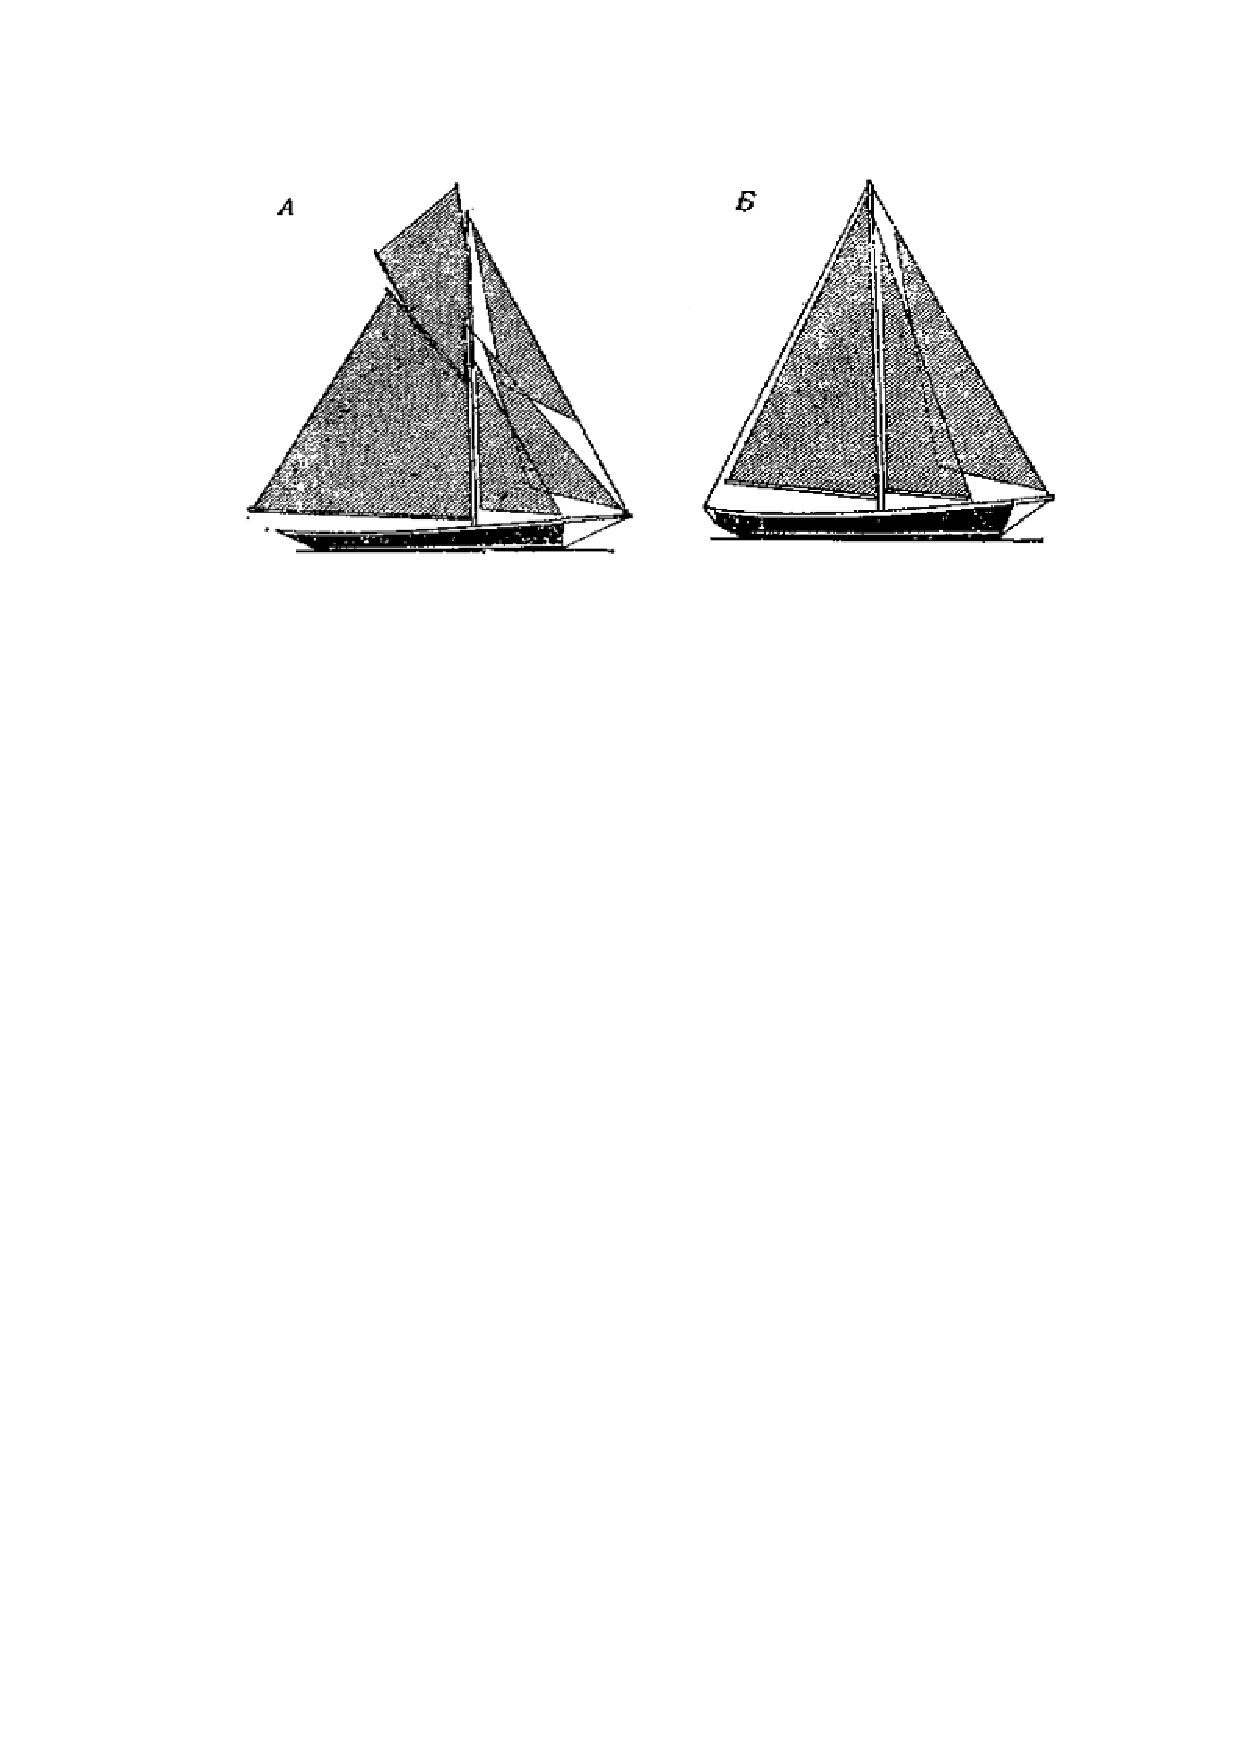
\includegraphics{Tendery}
	\protect\caption{\label{fig:14}Тендеры}
	\centering\small А \--- гафельный, Б \--- бермудский
\end{figure}


Когда парусность больше 60\--80\,$\mbox{м}^2$, её делят между большим числом
парусов. Тогда применяют тип вооружения, называемый тендером. Тендер
(рис.~\ref{fig:14})
несет в переднем треугольнике два или больше передних парусов, чем
и отличается от шлюпа. Эти паруса называются: \textbf{стаксель}\index{стаксель} (ближний
к мачте внизу), \textbf{кливер}\index{кливер} (впереди стакселя) и \textbf{кливер-топсель}\index{кливер-топсель}
(или \textbf{летучка}\index{летучка}) который ставится у самого топа мачты.

Тендеры, как и шлюпы, могут быть гафельными и бермудскими. Гафельные
тендеры чаще всего имеют мачту не цельную, а состоящую из двух частей:
мачты и \textbf{стеньги}\index{стеньга} (надставка к мачте сверху, которую можно
опускать).

\begin{figure}[htbp]
	\begin{centering}
		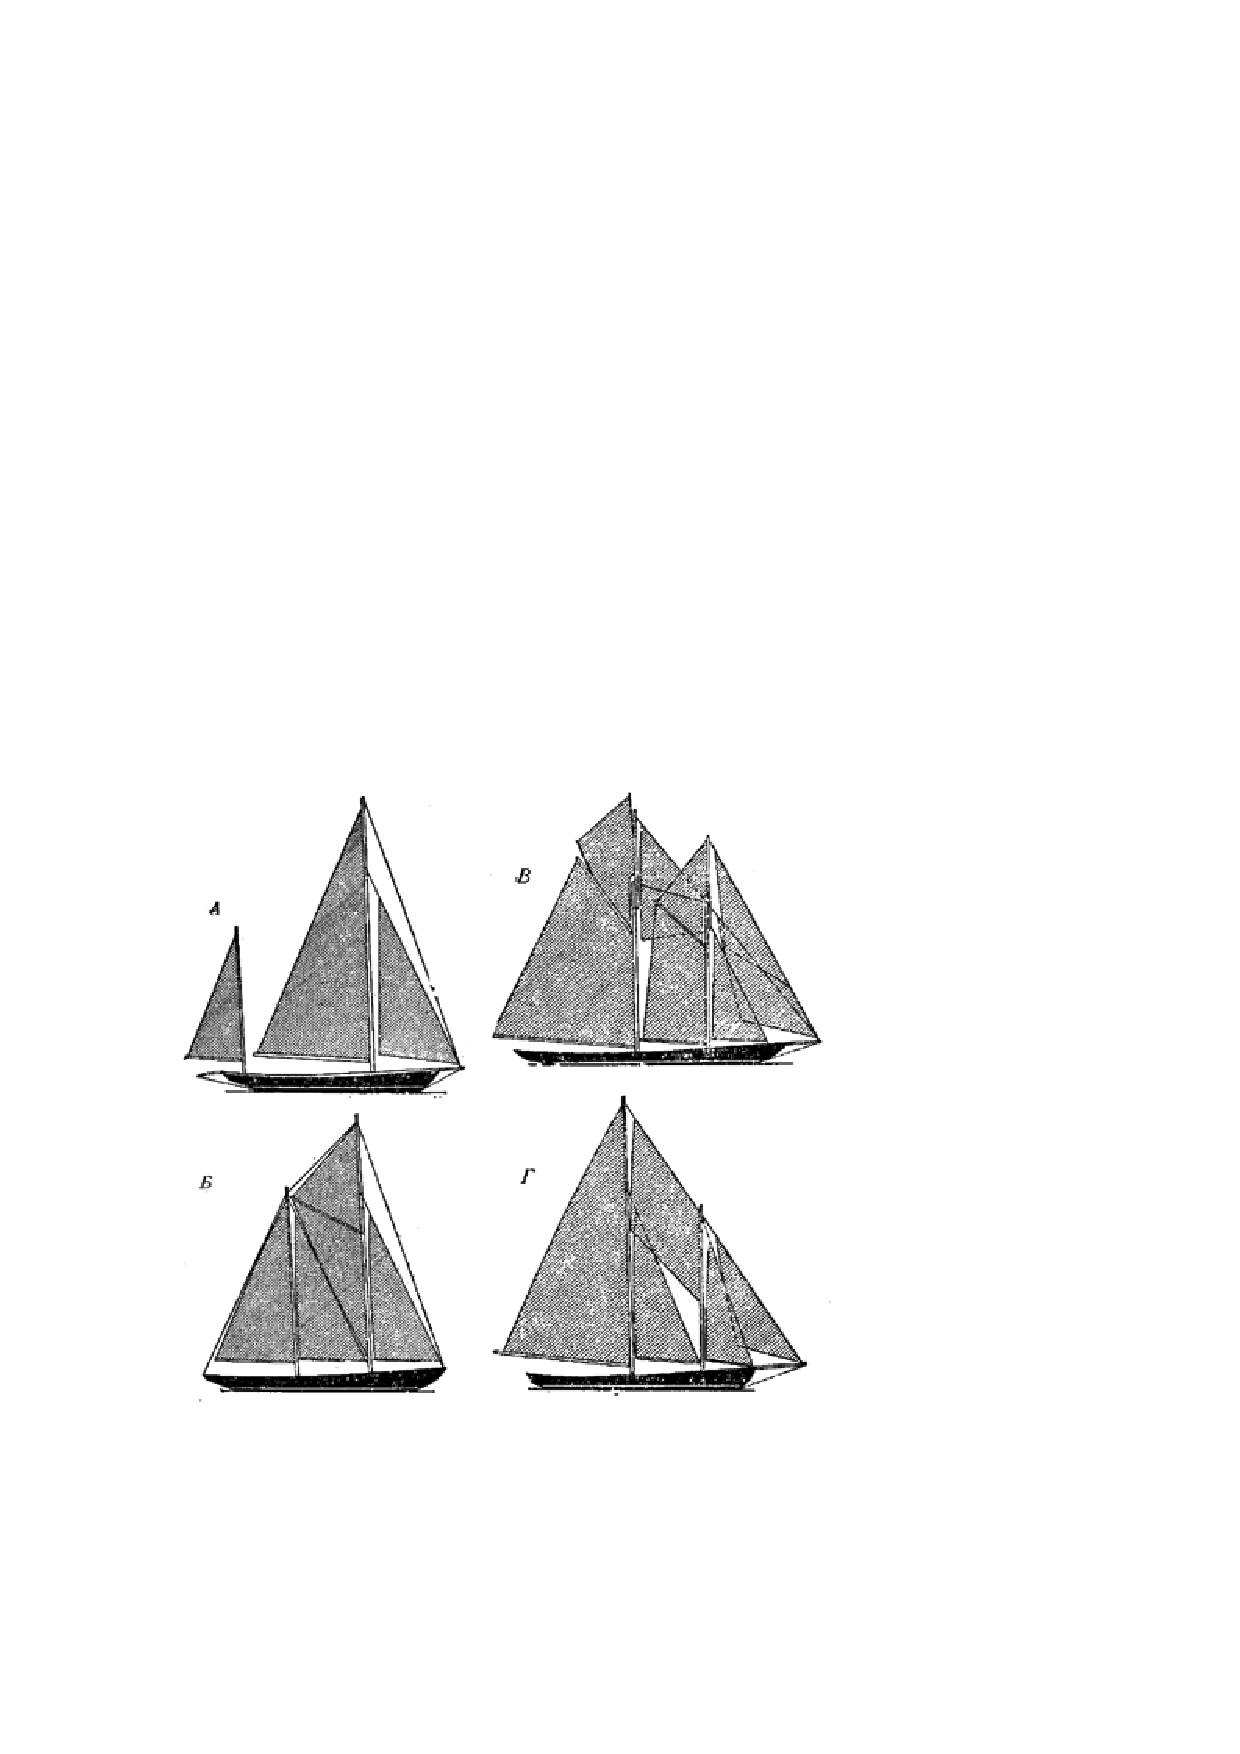
\includegraphics{Dvukhmachtovye_yakhty}
		\par
	\end{centering}
	\protect\caption{\label{fig:15}Двухмачтовые яхты}
	\centering{}\small А \--- бермудский иол; Б \--- стаксельный кэч; В \--- гафельная шхуна; Г \--- бермудская стаксельная шхуна
\end{figure}


Двухмачтовые вооружения (рис.~\ref{fig:15})
применяют на крупных крейсерских яхтах, где для уменьшения крена важно
иметь еще более низкую парусность, чем у тендеров. Кроме того, распределение
общей парусности на несколько парусов облегчает работу экипажа с ними,
что особенно важно на яхтах, совершающих дальние плавания. Чисто морские
преимущества двухмачтовых яхт весьма велики: уборкой тех или иных
парусов можно сразу уменьшить парусность, а комбинируя эти паруса,
можно приспособиться к большому диапазону сил ветра без взятия рифов.

Не очень крупные крейсерские яхты (50\--100\,$\mbox{м}^2$) в большинстве случаев
вооружают иолом или кэчем. Иол имеет короткую заднюю мачту (бизань-мачту),
которая установлена позади головки руля. Парус на этой мачте называется
бизанью. Иолы могут быть как гафельные, так и бермудские. Заметим,
что для всех двухмачтовых яхт с косыми парусами вид вооружения определяется
формой грота. Так, если иол имеет гафель-ный грот, он называется гафельным,
независимо от того, какая на нем бизань \--- гафельная или бермудская.
Площадь бизани на иоле обычно составляет 8-10\% общей площади парусности
яхты. 

\textbf{Кэч}\index{кэч} отличается от иола большей бизанью, имеющей площадь 15-
25\% от общей парусности, и тем, что бизань-мачта стоит впереди головки
руля.

Как и иол, кэч может быть бермудским или гафельным. Иногда кэч имеет
грот без гика, со шкотовым углом, находящимся у верхушки бизань-мачты.
Нижний промежуток заполняется тогда большим бизань-стакселем. Такие
кэчи называют стаксельными (рис.~\ref{fig:15},
\emph{б}). Бизань-стаксель может быть и у обычного кэча или иола,
только в этом случае его надо убирать при перекладывании грота с одного
борта на другой.

На иолах бизань скорее воздушный руль, чем парус, кроме того, в ряде
случаев иол удобнее с точки зрения работы экипажа на палубе и обзора
для рулевого.

Шхуна имеет заднюю мачту выше или равную передней. Передняя мачта
двухмачтовой шхуны называется фок-мачтой, а задняя \--- грот-мачтой.
Паруса называются соответственно фок и грот. Шхуны, как и прочие яхты,
могут быть гафельными и бермудскими. Бермудские шхуны часто вооружены
гафельным фоком (при равной с бермудским фоком высоте он может иметь
большую площадь парусности, чем последний). Существует разновидность
бермудской шхуны-стаксельная шхуна (рис.~\ref{fig:15},
\emph{г}). Эта шхуна не имеет фока. Промежуток между фок- и грот-мачтами
(междумачтовый четырехугольник) заполняется одним или несколькими
косыми треугольными парусами. Шхунами, как правило, вооружают самые
крупные яхты \--- парусностью более 150\--200\,$\mbox{м}^2$.

%--------------------------------------------------------------------------
%
%                  Спортивная классификация парусных яхт
%
%--------------------------------------------------------------------------

\section{Спортивная классификация парусных яхт}

Цель спортивной классификации \--- обеспечить возможности сравнения спортивных
достижений в парусных гонках, поскольку эти достижения в значительной
мере зависят от качества яхт.

\begin{figure}[htbp]
	\hfill{}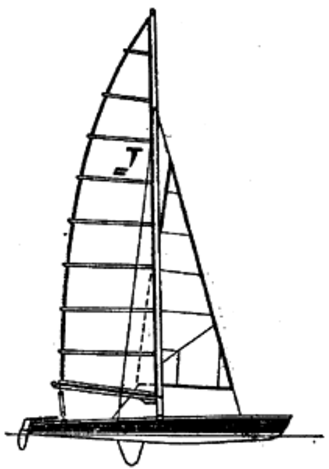
\includegraphics[scale=0.7]{Katamaran-monotip_Tornado}%
	\hfill{}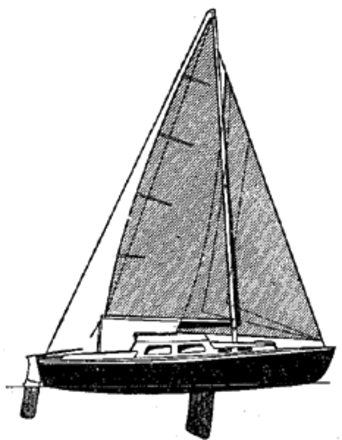
\includegraphics[scale=0.7]{Krejsersko-gonochnyj_shvertbot_svobodnogo_klassa_t3}%
	\hfill{}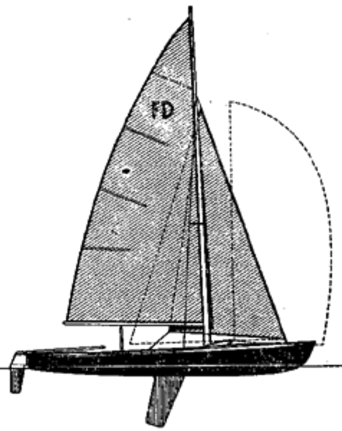
\includegraphics[scale=0.7]{Gonochnyj_shvertbot-monotip_Letuchij_Gollandets}%
	\hfill{}
	\par%
	\hfill{}%
	\begin{minipage}[t]{0.3\columnwidth}%
		\protect\caption{\label{fig:16}Катамаран\-/монотип <<Торнадо>>}%
	\end{minipage}%
	\hfill{}%
	\begin{minipage}[t]{0.3\columnwidth}%
		\protect\caption{\label{fig:17}Крейсерско\-/гоночный швертбот свободного класса ТЗ}%
	\end{minipage}%
	\hfill{}%
	\begin{minipage}[t]{0.3\columnwidth}%
		\protect\caption{\label{fig:19}Гоночный швертбот\-/монотип <<Летучий голландец>>}%
	\end{minipage}%
	\hfill{}

	\hfill{}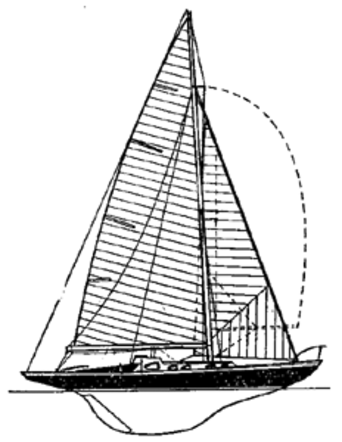
\includegraphics[scale=0.7]{L6}%
	\hfill{}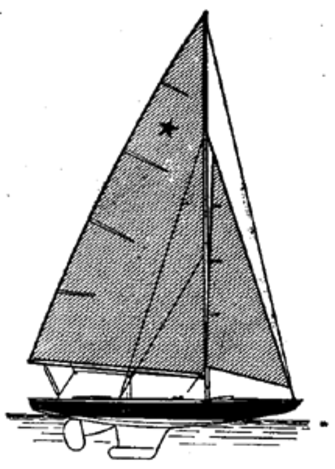
\includegraphics[scale=0.7]{Star_class}%
	\hfill{}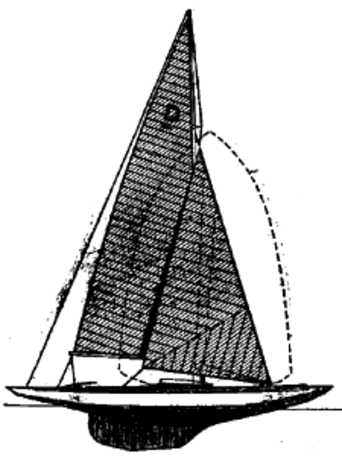
\includegraphics[scale=0.7]{Dragon}%
	\hfill{}

	\hfill{}%
	\begin{minipage}[t]{0.3\columnwidth}%
		\protect\caption{\label{fig:18}Крейсерско\-/гоночная яхта класса Л6}%
	\end{minipage}%
	\hfill{}%
	\begin{minipage}[t]{0.3\columnwidth}%
		\protect\caption{\label{fig:20}Яхта\-/монотип <<Звездного класса>>}%
	\end{minipage}%
	\hfill{}%
	\begin{minipage}[t]{0.3\columnwidth}%
\protect\caption{\label{fig:21}Гоночная яхта\-/монотип класса <<Дракон>>}%
	\end{minipage}%
	\hfill{}

	\hfill{}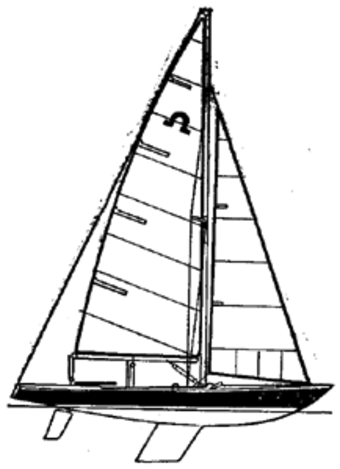
\includegraphics[scale=0.7]{Soling}%
	\hfill{}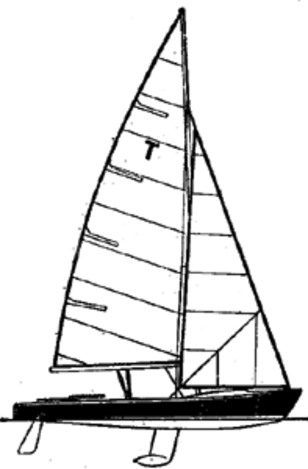
\includegraphics[scale=0.7]{Tempest}%
	\hfill{}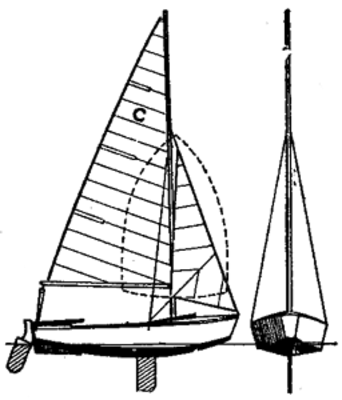
\includegraphics[scale=0.7]{Kadet}%
	\hfill{}

	\hfill{}%
	\begin{minipage}[t]{0.3\columnwidth}%
		\protect\caption{\label{fig:22}Гоночная яхта\-/монотип класса <<Солинг>>}%
	\end{minipage}%
	\hfill{}%
	\begin{minipage}[t]{0.3\columnwidth}%
		\protect\caption{\label{fig:23}Гоночная яхта\-/монотип класса <<Темпест>>}%
	\end{minipage}%
	\hfill{}%
	\begin{minipage}[t]{0.3\columnwidth}%
		\protect\caption{\label{fig:24}Детский швертбот\-/монотип класса <<Кадет>>}%
	\end{minipage}%
	\hfill{}
\end{figure}


Непосредственными задачами классификации являются:
\begin{itemize}
\item разделение спортивных парусных судов на классы (в зависимости от типа
и размера), чтобы в рамках каждого класса тем или иным способом ограничить
размеры и характеристики корпуса и вооружения яхты и тем самым обеспечить
достаточную безопасность плавания и сравнимость ходовых качеств;
\item выработка единых правил определения размеров яхт (правил обмера) и
порядка оформления документов, устанавливающих принадлежность яхты
к тому или иному классу (мерительных свидетельств).
\end{itemize}
Классификация яхт \--- довольно сложная задача. Типы яхт определяются
условиями их плавания (навигационными условиями) и уровнем развития
яхтенной техники. Классы яхт совершенствуются и видоизменяются по
мере развития парусного спорта. В свою очередь, классификация накладывает
отпечаток на развитие парусного спорта.

Сущность классификации заключается в ограничении размеров яхт и их
соотношений, влияющих на ходовые качества и мореходность.

Такими размерами являются:
\begin{itemize}
\item \textbf{длина яхты.}\index{яхта!размеры!длина} Чем она больше, тем меньше сопротивление корпуса,
а значит, яхта более быстроходна;
\item \textbf{ширина яхты.}\index{яхта!размеры!ширина} Чем шире яхта, тем больше, с одной стороны,
ее сопротивление, а с другой \--- остойчивость;
\item \textbf{осадка.}\index{осадка} Она оказывает большое влияние на остойчивость яхты
и её лавировочные качества, то есть способность идти под острым углом
к ветру (чем больше осадка, тем больше остойчивость и лучше лавировочные
качества яхты);
\item \textbf{высота надводного борта.}\index{яхта!размеры!высота надводного борта} Чем выше борт, тем яхта мореходнее
и лучше её обитаемость;
\item \textbf{водоизмещение (вес) яхты.}\index{яхта!размеры!вес}\index{яхта!размеры!водоизмещение} Чем больше водоизмещение, тем больше
сопротивление воды движению судна, но в то же время больше остойчивость
и мореходность;
\item \textbf{площадь парусности.}\index{яхта!размеры!площадь парусности} Чем она больше, тем при прочих равных
условия больше скорость яхты.
\end{itemize}
По степени ограничений классы яхт можно разбить на четыре основные
группы:
\begin{enumerate}
\item \textbf{Свободные классы}\index{класс!свободный}, в которых устанавливаются ограничения на
главные размеры яхт, а форма корпуса может быть произвольной. Такими
классами являются, например, советские национальные классы швертботов
М, Т2, ТЗ. 
\item \textbf{Формульные классы}\index{класс!формульный}, в которых ограничения по размерам связаны
главным образом с особыми формулами обмера. Эти формулы определяют
величину гоночного балла яхты, измеряемую обычно в линейных единицах
(метрах, футах). Формулы обмера подбирают таким образом, чтобы яхты,
имеющие одинаковый гоночный балл, теоретически имели бы и равные скорости.
Яхты одного класса, естественно, должны иметь одинаковый балл. К формульным
классам относятся яхты старого международного 5,5-метрового класса,
а также <<четвертьтонники>> и <<полутонники>> (К5 и Кб) и др. Формулы
обмера нашли главное применение для гандикапных классов крейсерско\-/гоночных
яхт (см. ниже).
\item \textbf{Монотипы}\index{класс!монотип}, которые строятся по одним и тем же чертежам при
строгом соблюдении правил постройки и обмера обеспечивающих идентичность
формы корпуса, размеров парусов и весовых характеристик, влияющих
на ходовые качества яхты. Монотипами являются швертботы <<420>>, <<470>>,
<<ОК>>, <<Финн>>, <<Кадет>> и <<Летучий голландец>>, а также килевые яхты
классов <<Солинг>>, <<Темпест>>, <<Дракон>>, <<Звездный>>. Большинство современных
малых гоночных яхт \--- монотипы.
\item \textbf{Гандикапные классы}\index{класс!гандикапный}, то есть классы яхт, обмеряемые по определенным
формулам, как и формульные классы. Разница состоит в том, что в гонках
участвуют яхты с разными гоночными баллами, а занятые места определяются
по так называемому исправленному времени. Исправленное время рассчитывается
таким образом: действительное время прохождения дистанции множат на
некоторый поправочный коэффициент, зависящий от гоночного балла. В
настоящее время в подавляющем большинстве стран, в том числе и в СССР,
приняты гандикапные классы крейсерско-гоночных яхт, обмеряемых по
международным правилам и формуле IOR.
\end{enumerate}
Кроме того, различают национальные и международные классы яхт. В каждой
стране могут появиться и появляются особые классы яхт, приспособленные
для плавания только в водах данной страны (или даже её отдельного
района, моря, озера). Такие классы называются национальными.

Многие удачные национальные классы начинают культивироваться в нескольких
странах. Хотя по существу они становятся уже международными, юридически
не являются таковыми. Международным классом считается класс, не только
получивший широкое распространение в ряде стран, но и официально признанный
Международным союзом парусных соревнований (ИЯРУ). Например, имевшийся
в советской классификации монотип Скандинавского парусного союза <<Фолькбот>>,
несмотря на широкое распространение во многих странах Европы, юридически
не является международным классом.

Международные классы подразделяются на группы А и В:
\begin{itemize}
\item группа А включает современные яхты с высокими характеристиками, в
проектах и правилах постройки которых использованы новейшие достижения
техники. Из этой группы выбирают олимпийские классы (для участия в
олимпийских регатах). В ней две подгруппы: A (R) \--- свободные или формульные
классы и А (О) \--- монотипы;
\item группа В включает классы, спроектированные более 20 лет назад, не
полностью соответствующие требованиям группы А, и классы, которым
международный статут присвоен вследствие их широкой популярности или
потому, что они обеспечивают хорошую подготовку к гонкам. В группе
В также две подгруппы: B(R) и В(О).
\end{itemize}
Каждый класс, кроме того, относится к определенной категории, в соответствии
с организационным построением класса.

К категории 1 относятся классы, которыми управляют ассоциации владельцев
яхт данного класса (под управлением понимается выпуск чертежей и правил
класса, организации гонок и т.\,д.).

К категории 2 относятся классы, определением правил и организацией
гонок в которых руководит непосредственно ИЯРУ через национальные
руководящие органы (федерации).

Помимо классов обычных яхт ИЯРУ предусматривает еще несколько классов
катамаранов, в частности свободный класс <<С>> и несколько монотипов.

Те международные классы, в которых проводятся олимпийские регаты,
называются олимпийскими.

Сейчас олимпийскими классами считаются:
\begin{itemize}
\item <<Финн>> \--- с 1952\,г.
\item <<Летучий голландец>> \--- с 1960\,г.
\item <<Темпест>> \--- с 1972\,г.
\item <<Солинг>> \--- с 1972\,г. Кроме принятых в настоящее время олимпийскими
классами были:
\item 8\-/метровый R\-/класс \--- во всех олимпиадах до 1936\,г. включительно;
\item  6\-/метровый R\-/класс \--- во всех олимпиадах до 1952\,г. включительно;
\item 5,5\-/метровый R\-/класс \--- с 1952 по 1968\,г.;
\item <<Звездный>> \--- с 1932 по 1972\,г.;
\item <<Дракон>> \--- с 1948 по 1972\,г.
\end{itemize}
Кроме того, в отдельные годы олимпийскими были: класс <<Олимпия-иол>> \--- в 1936\,г. и <<12 кв. м шарпи>> \--- в 1956\,г.

В Олимпиаде 1976\,г. будут участвовать кроме вышеназванных швертбот\-/двойка <<470>> (см. рис.~\ref{fig:13}, \emph{б}) и катамаран-монотип <<Торнадо>> (рис.~\ref{fig:16}).

Классификация яхт в СССР определяется едиными <<Правилами классификации,
постройки и обмера спортивных парусных яхт, принятых в СССР>>, которые
периодически пересматриваются и издаются Федерацией парусного спорта
СССР.

Действующая с 1973\,г. классификация предусматривает как советские
национальные. так и международные классы. Она включает десять международных
и четыре национальных класса яхт, в том числе два формульных класса
крейсерско-гоночных яхт с фиксированным гоночным баллом по международной
формуле IOR (<<четвертьтонники>> К5 с баллом 5,5 м и <<полутонники>>
К6 с баллом 6,6 м), а также два класса катамаранов. Таким образом,
отечественная классификация включает достаточное число классов яхт,
чтобы учитывать потребности всех водных районов страны в занятиях
всеми видами парусного спорта .

Советская классификация включает как чисто гоночные, так и крейсерско\-/гоночные
яхты.

Для гонок на швертботах предназначены суда международных классов <<Финн>>,
<<Летучий голландец>>, <<470>>, <<OK>>, <<420>> и юношеский
монотип <<Кадет>>, а также швертботы национального свободного класса
<<М>> с экипажем из трех человек. Эти швертботы имеют довольно большую
парусность \--- 26\,$\mbox{м}^2$ и сравнительно легкий длинный корпус \--- весом 200~кг и длиной 6,5~м.

Для крейсерских гонок и дальних плаваний по рекам, озерам и прибрежным
морским районам предназначены швертботы свободных крейсерско-гоночных
классов Т2 и ТЗ (рис.~\ref{fig:17}).

Для гонок и дальних плаваний в морских условиях советская классификация
предусматривает яхты формульных классов К5 (<<четвертьтонники>>)
и К6 (<<полутонники>>). Разнообразные крейсерско-гоночные и крейсерские
яхты для участия в гонках должны быть обмерены и отнесены к одному
из принятых у нас международных гандикапных классов по правилам IOR.
Например, яхта старого класса Л6 относится ко II классу IOR (рис.~\ref{fig:18}).
Основные сведения о яхтах советской классификации даны в приложении
1.

В классификацию включены наиболее распространенные международные классы
яхт. К ним относятся в первую очередь олимпийские классы <<Финн>>,
<<470>>, <<Летучий голландец>>, <<Темпест>> и <<Солинг>>.

Швертботы-одиночки класса <<Финн>> (см. рис.~\ref{fig:12},
г) очень распространены (конструктор швед Р. Сарби \--- 1950\,г.).

Очень быстроходный швертбот \--- монотип <<Летучий голландец>> (рис.~\ref{fig:19}),
на котором ходят два человека (конструктор голландец У. Ван-Эссен).

Яхта <<Звездного класса>>, сконструированная американцем Гарднером в 1911\,г. (рис.~\ref{fig:20}), очень интересна для гонок. Ею управляют два человека. Вследствие известной перегруженности яхты парусами от экипажа требуется большая ловкость, сработанность и отличная физическая подготовка. Этот класс существует с 1911\,г.

Килевой монотип <<Дракон>> (рис.~\ref{fig:21})
представлят собой деревянную, сравнительно тяжелую яхту с очень маленькой
рубкой \--- козырьком и просторным кок-питом. Ходят на ней три человека.
<<Дракон>> спроектирован в 1929\,г. норвежцем И. Анкером.

Класс <<Солинг>> (рис.~\ref{fig:22}) \--- новый олимпийский класс. Это яхта-монотип с экипажем в три человека,
имеющая пластмассовый корпус, изготовленный по стандартной форме (матрице),
что позволяет обеспечить сравнительно высокую идентичность обводов.
Конструктором яхты является норвежец Линге.

Яхта класса <<Темпест>> (рис.~\ref{fig:23})
является, по существу, швертботом, в швертовыи колодец которого вставлен
узкий шверт, имеющий на конце обтекаемый бульб весом около 200 кг.
Этот бульб-киль легко вынимается из колодца, что облегчает транспортировку
яхты. Па яхте <<Темпест>> ходят двое: рулевой и шкотовый. Конструктор
ее \--- англичанин Ян Проктор.

Швертбот-монотип двойка <<470>> (французский национальный класс, международный
с 1970\,г.) спроектирован Андре Корню. Хорошо ходит при весе экипажа
до 150 кг (см. рис.~\ref{fig:13}, \emph{б}).

Кроме того, классификация включает следующие классы для детей юношей;
\begin{itemize}
\item класс <<ОК>> (О'кэй) \--- распространен как юношеский швертбот-одиночка;
\item международный юношеский класс <<Кадет>> \--- разработан в Англии конструктором
Д. Холтом в 1947\,г. (рис.~\ref{fig:24}) \--- швертбот-двойка;
\item детский монотип-одиночка <<Оптимист>> \--- маленький швертбот\-/плоскодонка,
простой в самодеятельной постройке; <<Оптимист>> является монотипом
Скандинавского парусного союза и распространена во многих странах;
\item монотип-двойка <<420>> французского конструктора Мори; яхты этого международного
класса очень быстроходны и интересны; среди них разыгрываются первенства
Европы и ряда стран.
\end{itemize}
<<Правила классификации, постройки и обмера>> включают также правила
обмера, правила несения отличительных знаков класса, а также частные
правила по отдельным классам.

\textbf{Правила обмера}\index{обмер!правила} предписывают, каким образом измерять определяющие
класс размеры яхты и площадь её парусности. Обмером судов занимаются,
специально выделенные спортивными организациями лица \--- официальные
мерители. Измерив судно и определив, входит ли оно в тот или иной
класс, меритель выдает владельцу яхты \textbf{мерительное свидетельство}\index{свидетельство!мерительное}
\--- документ, подтверждающий соответствие судна классу и фиксирующий
его измеряемые размеры и другие необходимые данные (год и место постройки,
конструктор, владелец, порт приписки и т.\,п.). Свидетельство регистрируется
в Спортсудорегистре Комитета по физической культуре и спорту СССР,
где на каждый класс заведены специальные мерительные книги, после
чего оно становится действительным. Яхта, не имеющая такого мерительного
свидетельства, не имеет права участвовать в классных гонках.

Обмеренные и классифицированные яхты носят на парусах отличительные
знаки своего класса и номера, соответствующие порядковому номеру регистрации
данной яхты в Общесоюзной мерительной книге. Например, швертбот национального
класса ТЗ, зарегистрированный в классе под №75, должен нести на парусе
следующее обозначение:%
\begin{tabular}{c}
\textbf{ТЗ}\tabularnewline
\hline 
\textbf{75}\tabularnewline
\end{tabular}

Яхты международных классов перед номером несут латинские буквы, означающие
государственную принадлежность: для СССР это буквы <<SR>>. Таким образом,
яхта международного класса <<Темпест>> №25 будет нести на парусе знак:
\begin{tabular}{c}
\textbf{Т}\tabularnewline
\hline 
\textbf{RUS25}\tabularnewline
\end{tabular}

Цифры и буквы должны быть стандартного размера. Их нашивают в определенном
месте с обеих сторон грота таким образом, чтобы при просвечивании
паруса цифры и буквы не накладывались друг на друга.

Яхта, не имеющая на гроте соответствующих обозначений, не имеет права
выхода и при участии в гонках на финише не принимается.

Гандикапные крейсерско-гоночные яхты обмеряются по специальным правилам
и формуле, по которой определяется их гоночный балл. В соответствии
с этим обмером каждая такая яхта относится к определенному классу
IOR. Между яхтами каждого гандикапного класса проводятся гонки с уравнением
шансов (гандикап). Гандикапные яхты несут на парусах римскую цифру,
обозначающую номер их класса IOR, государственное обозначение (как
международные классы) и порядковый номер. Например, яхта IV класса
№3 будет нести номер:%
\begin{tabular}{c}
\textbf{IV}\tabularnewline
\hline 
\textbf{RUS3}\tabularnewline
\end{tabular}

Неклассные швертботы и яхты служат для учебной работы и крейсерских
плаваний. Они не подлежат регистрации во всесоюзном масштабе и регистрируются
только в своем городе. Им присвоена буква <<Н>>, под которой нашивается
порядковый номер для данного города.

Каждая яхта, участвующая в гонках, как мы уже говорили, должна иметь
действительное мерительное свидетельство, и на её корпусе и рангоуте
должны быть нанесены так называемые обмерные марки \--- отметки, ограничивающие
крайние точки размеров парусов и некоторых размеров корпуса. Порядок
постановки марок приведен в <<Правилах классификации, постройки и обмера
спортивных парусных яхт, принятых в СССР>> и в частных правилах классов.

%--------------------------------------------------------------------------
%
%                                   * * *
%
%--------------------------------------------------------------------------

\section*{{*}{*}{*}}

Выше были рассмотрены советская и международная классификация яхт.
В целом ряде стран существуют свои, более или менее развитые национальные
классификации, которые предусматривают интересные классы.

Не касаясь всех зарубежных классификаций и их построения детально,
отметим, что они имеют более <<эмпирический>> характер, и выбор классов
в них определяется, по-видимому, просто ходом событий в парусном мире.
Ряд стран (особенно малых) вообще не имеет собственных классификаций
и национальных классов яхт, применяя в своей практике международные
и национальные классы других стран.

Обращает на себя внимание большое количество монотипов в классификациях
почти всех зарубежных стран.

Познакомимся с некоторыми наиболее интересными и популярными зарубежными
классами яхт.

К таким классам относятся прежде всего чрезвычайно популярные во многих
странах Восточной и Центральной Европы крейсерские швертботы с парусностью
15\--20\,$\mbox{м}^2$ и швертботы\-/монотипы <<Пират>>. Наш швертбот класса <<Т>>,
по существу, тоже является <<продуктом>> развития европейских крейсерских
швертботов.

Популярный в Европе швертбот-монотип для двух человек <<Пират>> имеет
обводы типа <<Шарпи>> и парусность 10\,$\mbox{м}^2$. Он очень устойчив, удобен
для первоначального обучения и интересен в гоночном отношении. Особенно
много <<Пиратов>> в ГДР, Чехословакии, Венгрии, Польше.

Из свободных классов США некоторый интерес представляют гоночные швертботы
типа <<Скоу>>. Это слово буквально переводится на русский язык как <<шаланда>>.
Швертботы <<Скоу>> \--- низкобортные, сравнительно широкие яхты, имеющие
транцевый нос и обычно два шверта. Именно от них пошли у нас в свое
время на Волге и в Ленинграде двухшвертовые швертботы типа <<Ри-Ри>>,
и именно поэтому они раньше назывались у нас <<американцами>>.

В большинстве стран в национальных классах преобладают швертботы и
очень мало килевых яхт. Так, в Италии из семи национальных классов
шесть швертботов, во Франции \--- все национальные классы швертботы,
в Англии \--- добрых 90\% и т.\,д. Это объясняется тем, что швертботы
дешевле в постройке, более <<чувствительны>> к навигационным условиям,
и поэтому в каждой стране вследствие особенностей различных бассейнов
возникают свои, приспособленные к условиям данной страны (или даже
ее района) классы. Дешевизна и удобства эксплуатации швертботов, не
требующих дорогих эллингов, способствуют появлению множества национальных
классов.

Что касается килевых яхт национальных классов, то их очень мало прежде
всего потому, что номенклатура международных классов достаточно велика
и обеспечивает практически суда на любой вкус. И хотя особой необходимости
в создании килевых яхт национальных классов нет, в некоторых странах
такой класс развивается. К ним относится, например, финский класс
<<А>>, шведский крейсерский монотип <<Фолькбот>> и некоторые другие.

Сравнительно короткий и широкий <<Фолькбот>> с обшивкой <<кромка на кромку>>,
представляющий собой удачную яхту для крейсерства с малым экипажем,
очень популярен в Скандинавских странах и как гоночное судно \--- на
международных регатах в Сандхамне и Гетеборге (Швеция) на старт выходят
сотни этих монотипов.

%===========================================================================
%
%                        Устройство и вооружение яхты
%
%===========================================================================

\chapter{Устройство и вооружение яхты}

%--------------------------------------------------------------------------
%
%                                  Корпус
%
%--------------------------------------------------------------------------

\section{Корпус}

Корпус любого судна состоит из \textbf{набора}\index{набор} \--- деталей, образующих
основу, скелет судна, \textbf{обшивки}\index{обшивка} \--- оболочки, покрывающей его
днище и борта, и \textbf{палубного настила}\index{настил!палубный}, образующего палубу судна.

В зависимости от материала, из которого изготовлен корпус яхты, различают:
\begin{itemize}
\item \textbf{деревянные яхты}\index{яхта!деревянная} \--- у них набор, палуба и обшивка сделаны из
дерева; разновидностями деревянных яхт являются яхты, обшивка и палуба
которых сделаны из фанеры (фанерные яхты), а также яхты, обшивка которых
выклеена из шпона-тонких узких полос лущеной древесины;
\item \textbf{металлические яхты}\index{яхта!металлическая}, у которых набор и обшивка сделаны из
стали или легких сплавов;
\item \textbf{яхты композитной (смешанной) постройки}\index{яхта!композитной постройки}, у которых большая
часть набора (обычно поперечный набор) сделана из стали, а обшивка
и палуба из дерева;
\item \textbf{пластмассовые яхты}\index{яхта!пластмассовая}, сделанные из слоистых пластиков, обычно
на основе стекловолокнистых материалов, пропитанных твердеющими синтетическими
смолами.
\end{itemize}
В последние годы предпринимались попытки строить яхты из армированного
металлической сеткой или стекловолокном цемента (армо- и стеклоцементные
яхты). Эти яхты не получили распространения, так как они тяжелее обычных,
во всяком случае при малых и средних размерах. Видимо, трудно ожидать
появления хороших крейсерско-гоночных яхт из армоцемента (не говоря
уже о гоночных) длиной менее 12\--15 м, хотя бы в малой степени способных
конкурировать с обычными яхтами.

Яхты малого и среднего размера чаще всего бывают деревянными или пластмассовыми,
крупные яхты \--- обычно композитной постройки или металлические.

В настоящее время большинство гоночных яхт строится из стеклопластика.
Так, современные гоночные яхты международных классов <<Солинг>>, <<Темпест>>,
большая часть швертботов классов <<Финн>>, <<420>>, <<Кадет>>, а также значительное
число крейсерско-гоночных яхт <<четвертьтонного>> и <<полутонного>> классов
- стеклопластиковые Хотя стоимость стеклопластиковых яхт, как правило,
выше деревянных из-за больших затрат на технологическую оснастку и
материалы, затраты на их ремонт и содержание существенно меньше. Кроме
того, большая прочность стеклопластика позволяет уменьшить вес конструкции
и строить более легкие суда. К достоинствам стеклопластиковых яхт
надо отнести и такие немаловажные качества, как отсутствие течи и
малое поглощение влаги .Однако у нас в стране деревянные яхты все
еще широко распространены. Конструкция их типовая, поэтому дальше
мы рассматриваем в качестве основного устройство именно деревянных
яхт.

Следует отметить также, что для крейсерских и крейсерско-гоночных
яхт широко применяются легкие сплавы, стойкие в морской воде (например,
алюминиево\-/магниевые), а для малых и средних яхт \--- фанера и шпон.

%--------------------------------------------------------------------------
%
%                  Основные детали набора деревянной яхты
%
%--------------------------------------------------------------------------

\section{Основные детали набора деревянной яхты}

Основной деталью набора является \textbf{киль-брус}\index{киль-брус}, проходящий вдоль
судна по его диаметральной плоскости (рис.~\ref{fig:25}
и \ref{fig:26}).
Киль представляет собой основную нижнюю продольную связь судна. Спереди
к килю присоединяется \textbf{форштевень-брус}\index{форштевень-брус} (или набор брусьев),
определяющий форму носа или носового свеса. К кормовой части киля
при помощи \textbf{старнкницы}\index{старкница} крепится \textbf{ахтерштевень}\index{ахтерштевень} \--- вертикальный
брус, к которому у яхты с транцевой обрезной кормой крепится \textbf{транец}\index{транец},
а у яхты, имеющей кормовой свес (рис.~\ref{fig:25}), навешивается руль. Транец
по кромкам усилен обвязкой \--- деревянной рамой, к которой крепятся
концы обшивки и сам транец.

\begin{figure}[htbp]
\centering
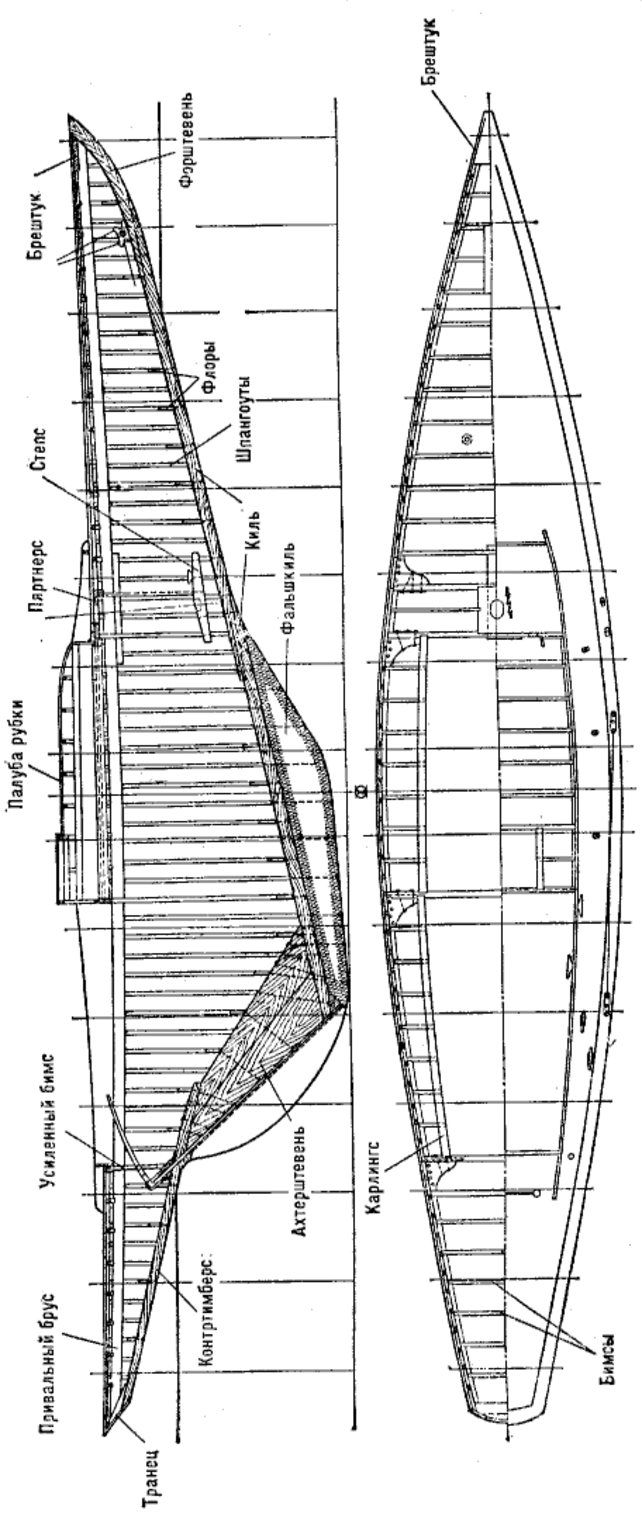
\includegraphics[scale=0.85]{Korpus_kilevoy_yakhty}
\protect\caption{\label{fig:25}Конструкция корпуса килевой яхты}
\end{figure}


У килевой яхты, имеющей кормовой свес, к ахтерштвеню сверху крепится
продольный брус \--- \textbf{контртимберс}\index{контртимберс}. Кница, крепящая к контртимберсу
транец, называется транцевой.

Снизу к килю болтами крепится балластный киль (фальшкиль), отливаемый
из свинца или чугуна. Свинцовый фальшкиль занимает меньший объем из-за
большого удельного веса свинца и оказывает меньшее сопротивление движению,
чем чугунный, и поэтому всегда предпочтительнее. Чтобы опустить фальшкиль
ниже и тем самым повысить остойчивость и лавировочные качества яхты,
между килем и фальшкилем иногда ставят \textbf{дейдвуд}\index{дейдвуд} \--- набор кусков
(как говорят, штук) дерева.

Киль, собранный со штевнями, транцем и дейдвудами, называется \textbf{закладкой}\index{закладка},
так как постройка судна начинается со сборки и установки всех этих
частей на стапель-место, где строится судно.

У стеклопластиковых яхт киля и штевней как таковых нет, а необходимую
прочность создает утолщенная обшивка в тех местах, где на деревянной
яхте стоят части закладки.

Если киль можно назвать хребтом яхты, то ребрами её являются \textbf{шпангоуты}\index{шпангоут},
поддерживающие обшивку. Обычно шпангоуты состоят из двух симметричных
ветвей, скрепленных внизу металлическими или деревянными флорами (рис.~\ref{fig:27}).
Шпангоуты бывают гнутые и жесткие (усиленные). Гнутые шпангоуты, как
правило, выгибаются по заранее установленной на стапеле отшивке и
приклепываются к ней. Их делают из ясеня или дуба.

Жесткие шпангоуты обычно ставят на закладку в стапеле до постановки
обшивки и делают из дерева (дуба или ясеня) или из стальных катаных
профилей (обычно углового профиля).

На современных деревянных яхтах гнутые и жесткие деревянные шпангоуты
выклеивают из тонких реек и устанавливают до постановки обшивки. Такая
конструкция шпангоутов обеспечивает большую прочность, поэтому нет
необходимости применять натесные, то есть собранные из отдельных кусков
(футоксов), жесткие шпангоуты, как это делалось на старых яхтах и
крупных деревянных судах. Однако на яхтах-шарпи шпангоуты удобнее
собирать из футоксов. Типовая конструкция шпангоута яхты-шарпи показана
на рис.~\ref{fig:28}.

\begin{figure}[htbp]
\begin{centering}
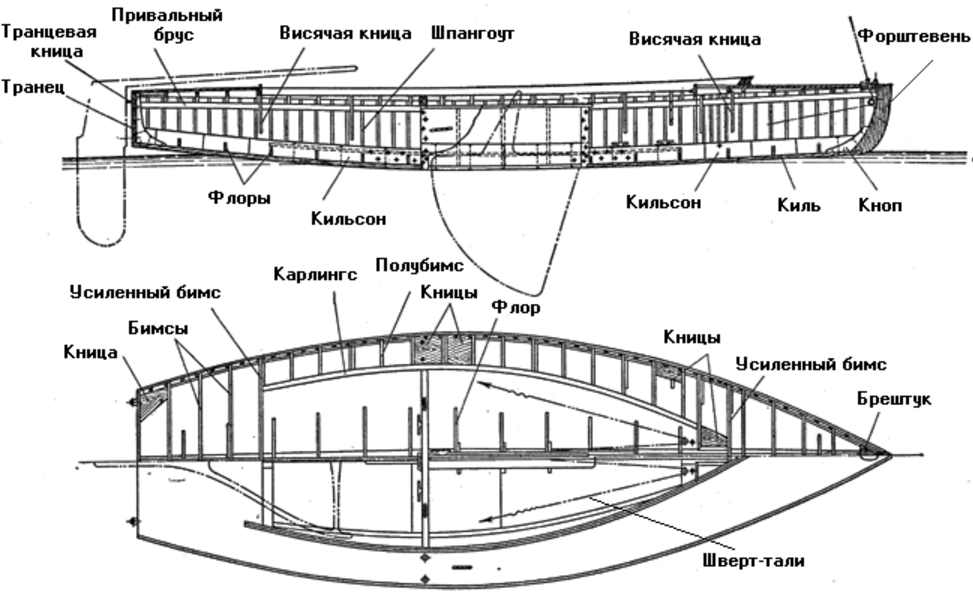
\includegraphics{Korpus_shvertbota}
\par\end{centering}

\protect\caption{\label{fig:26}Конструкция корпуса швертбота}
\end{figure}


Расстояние между шпангоутами называется \textbf{шпацией}\index{шпация}. В районе
мачты, где к корпусу приложены большие усилия от вооружения, шпангоуты
ставят чаще. Кроме того, перед мачтой и за ней устанавливают усиленные
шпангоуты большого сечения.

Нижние концы шпангоутов, примыкающие к килю, соединяют между собой
и крепят к килю флорами. У мелких килевых яхт и швертботов флоры делают
из твердого дерева, а у более крупных \--- кованые из полосовой стали
или сварные из листовой стали. Флоры крепят к килю и шпангоутам заклепками
или болтами, а на современных яхтах еще и склеивают с ними водостойким
клеем. В нижней части флоров прорезаются отверстия, для того чтобы
вода, попавшая внутрь корпуса, могла стекать в самую нижнюю часть
корпуса. Эти отверстия называют водопротоками или \textbf{шпигатами}\index{шпигат}.

\begin{figure}[htbp]
\begin{centering}
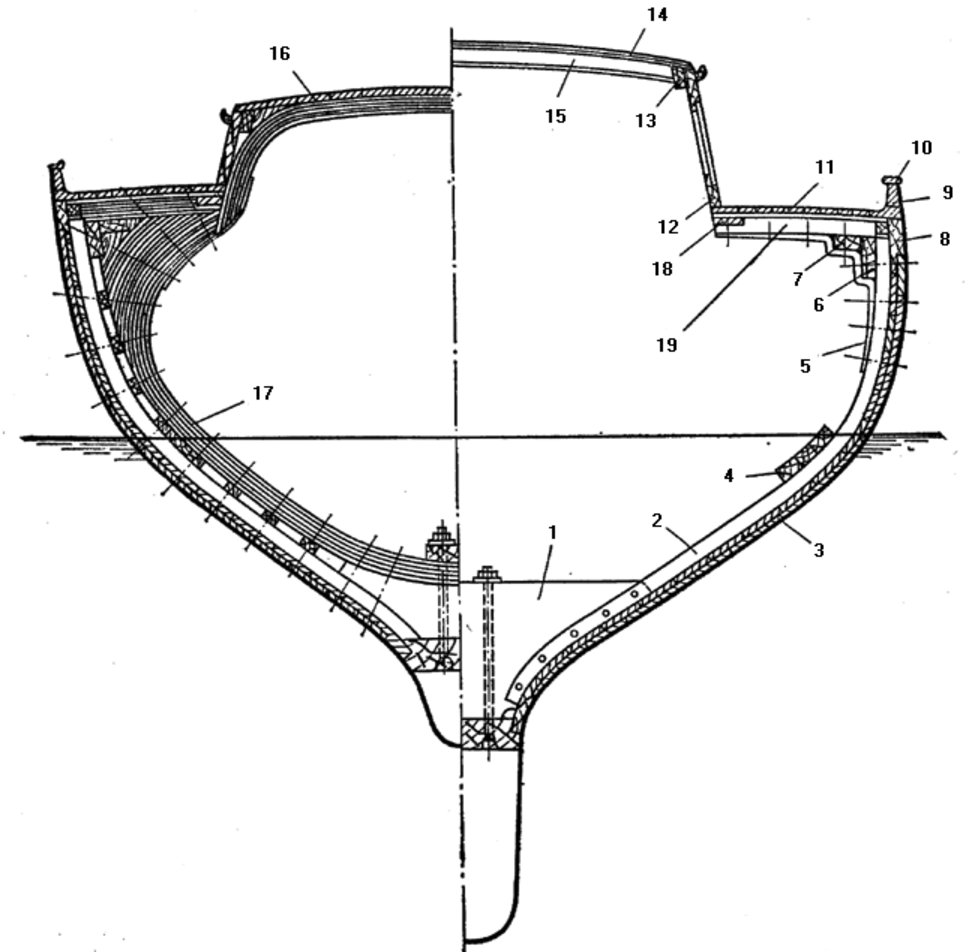
\includegraphics{Razrez_1}
\par\end{centering}

\protect\caption{\label{fig:27}Поперечный разрез деревянной кругло-шпангоутной яхты}


\begin{centering}\small
1~---~флор; 2~---~шпангоут; 3~---~двойная продольная обшивка; 4~---~скуловой
стрингер; 5~---~висячая кница; 6~---~привальный брус; 7~---~шельф; 8~---~ширстрек;
9~---~фальшборт; 10~---~планширь; 11~---~палубный настил; 12~---~комингс рубки;
13~---~шельф; 14, 16~---~крыша рубки; 15~---~бимс; 17~---~усиленный рамный
шпангоут; 18~---~карленгс; 19~---~полубимс
\par\end{centering}

\end{figure}


Основное назначение \textbf{флоров}\index{флор} \--- скрепление ветвей шпангоутов,
соединение их с килем и укрепление днищевой части обшивки. На флоры
у швертботов и мелких килевых яхт обычно кладутся слани. На некоторых
швертботах поверх флоров вдоль киля кладется \textbf{кильсон}\index{кильсон} \--- продольный
брус, дополнительно укрепляющий корпус в продольном направлении (рис.~\ref{fig:26}).

Кроме киля и кильсона для усилений продольной прочности яхты служат
также \textbf{стрингеры и привальные брусья}\index{стрингер}\index{брус!привальный}. Стрингеры кладут в районе
скулы изнутри, поверх шпангоутов, и соединяют с ними, увеличивая таким
образом жесткость обшивки. У яхт с угловатым миделем деталь, соединяющая
между собой шпангоуты по скуле, называется скуловым стрингером (рис.~\ref{fig:28}).
Привальные брусья (рис.~\ref{fig:25}\--\ref{fig:28})
бывают внутренние и внешние. Внутренние привальные брусья расположены
по самому верху шпангоутов и тянутся от форштевня до транца. Их проклепывают
через шпангоуты к обшивке. Это не только важнейшая продольная связь,
но и опора для палубного набора. Впереди привальные брусья связаны
между собой и штевнем брештуком \--- толстой горизонтальной деревянной
или металлической кницей (рис.~\ref{fig:25}
и \ref{fig:26}).
В корме привальные брусья также связываются с транцем горизонтальными
кницами. Внешние привальные брусья идут снаружи обшивки по борту и
предназначены для предохранения обшивки от повреждения.

\begin{figure}[htbp]
\begin{centering}
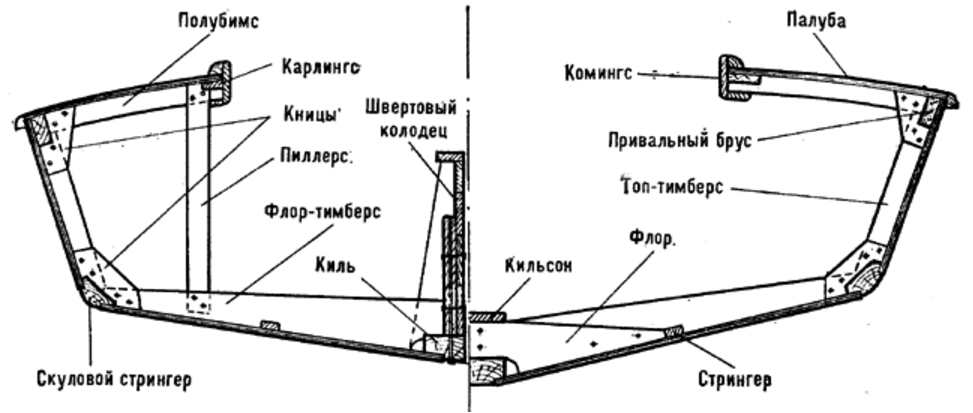
\includegraphics{Razrez_2}
\par\end{centering}

\protect\caption{\label{fig:28}Поперечный
разрез швертбота-шарпи с фанерной обшивкой}


\end{figure}


На гоночных яхтах не ставят внешние привальные брусья, так как они
увеличивают сопротивление судна в воде. Однако на малых крейсерах
(например, на швертботах класса ТЗ) иногда их все же ставят и снабжают
металлической оковкой для предохранения от раскалывания.

Иногда внутренний привальный брус имеет усиления-короткие брусья,
идущие рядом и склеенные или надежно скрепленные с ним. Они называются
\textbf{шельфами}\index{шельфы}. Шельфы обычно ставят в районе размещения мачты,
там, где проходят \textbf{вантпутенсы}\index{вантпутенсы} \--- узлы для крепления вант.

Палубный набор составляют \textbf{бимсы}\index{бимсы} \--- поперечные балки, концами
положенные на привальные брусья. На бимсы настилается палуба.

По границам вырезов в палубе (люков, кокпитов, надстроек) ставят \textbf{усиленные
бимсы}\index{бимсы!усиленные} \--- большего сечения. Бимсы обычно делают из сосны или ели, а
на усиленные бимсы нередко идет дерево твердых пород (дуб, ясень и
др). Усиленные бимсы ставят также спереди и сзади мачты. Для большей
жесткости их связывают со шпангоутами и обшивкой вертикальными (висячими)
кницами из криворослого дерева или стали (кованой или листовой).

В тех местах, где в палубе сделаны вырезы (для надстроек, кокпитов,
люков и т.\,п.), ставятся полубимсы. Внутренние концы полубимсов лежат
на карлингсах-продольных брусьях, которые, в свою очередь, опираются
на соответствующие усиленные бимсы, ограничивающие вырез в палубе.

Чтобы увеличить жесткость палубного набора; концы усиленных бимсов
перевязывают с привальными брусьями горизонтальными кницами. Мачтовые
бимсы в середине связаны толстой подушкой, подкрепляющей палубу в
том месте, где сделан \textbf{пяртнерс}\index{пятнерс} \--- отверстие для прохода мачты.
Если мачта ставится на палубу, то в этом месте делают обязательно
переборки, связывающие усиленные бимсы со шпангоутами, а сами бимсы
- большего сечения, чем обычные усиленные бимсы.

Бимсы и полубимсы могут опираться на пиллерсы \--- вертикальные или наклонные
деревянные стойки, нижним концом связанные с флорами или стрингерами
(рис.~\ref{fig:28}).
Пиллерсы увеличивают прочность палубного набора и противодействуют
усилиям, оказываемым на палубу сверху вниз. В месте укрепления мачты
могут возникать усилия, направленные снизу вверх, оказываемые, например,
стоячим и бегучим такелажем. Чтобы разгрузить палубу от таких усилий,
ставят \textbf{струны}\index{струны} \--- стальные прутки, соединяющие пяртнерсовую
подушку или бимсы с флорами или килем.

На больших судах поверх бимсов под палубный настил кладут \textbf{палубные
шины}\index{шины!палубные} \--- стальные полосы, идущие от борта к борту под углом к бимсам.
Такие же полосы кладут под обшивку поверх шпангоутов и под углом к
ним (их называют диагональными шинами). Шины связывают между собой
бимсы и шпангоуты, увеличивая прочность и жесткость корпуса.

На пластмассовых яхтах палубный набор зачастую отсутствует, а необходимые
жесткость и прочность палубы обеспечивают отформованные на обшивке
и палубе выступы (гофры, зиги). Иногда палубу делают из двух тонких
слоев стеклопластика с заформованным между ними слоем пенопласта (так
называемая сэндвичевая или трехслойная конструкция).


%--------------------------------------------------------------------------
%
%                         Обшивка и палубный настил
%
%--------------------------------------------------------------------------

\section{Обшивка и палубный настил}

Обшивка деревянной яхты обычной конструкции может быть выполнена вгладь,
кромка на кромку, может быть и на пазовых рейках и диагональной (рис.~\ref{fig:29}).

\begin{figure}[htbp]
\begin{centering}
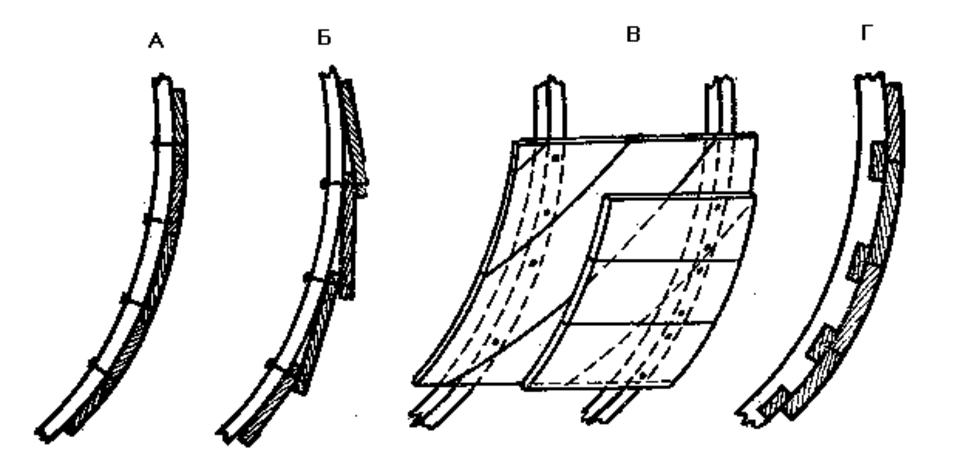
\includegraphics{Vidy_obshivki}
\par\end{centering}

\protect\caption{\label{fig:29}Виды обшивки}


\begin{centering}\small
А \--- вгладь; Б \--- кромка на кройку; В \--- диагональная; Г \--- на пазовых рейках
\par\end{centering}

\end{figure}


Чаще всего яхты обшивают \textbf{вгладь}\index{обшивка!вгладь}. Каждая доска обшивки от
носа до кормы называется \textbf{поясом}\index{пояс}. Если яхта большой длины,
то пояса стыкуются из нескольких досок, склеиваемых или соединяемых
изнутри подушкой на заклепках. Каждый пояс приклепывается к шпангоутам
медными (или из оцинкованной мягкой стали) заклепками, под которые
подкладывают шайбы; иногда его прикрепляют шурупами.

Стыки поясов обшивок по кромкам называются \textbf{пазами}\index{паз}. Чтобы
корпус был водонепроницаемым, пазы должны быть очень хорошо пригнаны.
На современных яхтах широко применяют склейку поясов по пазам водоупорным
клеем. Такая обшивка придает корпусу большую жесткость, так как пояса
совершенно не сдвигаются относительно друг друга. Раньше на яхтах
пазы иногда конопатили.

Нижний пояс обшивки, непосредственно примыкающий к килю, называется
\textbf{шпунтовым}\index{пояс!шпунтовый}, так как он входит в паз киля, называемый \textbf{шпунтом}\index{шпунт};
самый верхний \--- \textbf{ширстреком}\index{ширстрек}. На некоторых яхтах ширстрек в
верхней части утолщают и делают из твердого дерева.

Обшивка \textbf{кромка на кромку}\index{обшивка!кромка на кромку} на яхтах встречается редко, так
как выступающие стыки поясов создают лишнее сопротивление корпуса.
Такая обшивка применена на монотипах <<Фолькбот>>.

Обшивки на \textbf{пазовых рейках}\index{обшивка!на пазовых рейках} и \textbf{диагональная}\index{обшивка!диагональная} обеспечивают
высокую прочность и лучшую водонепроницаемость корпуса, но из-за определенной
сложности выполнения и дороговизны встречаются редко.

Для сравнительно небольших яхт применяют обшивку из \textbf{шпона}\index{обшивка!из шпона},
то есть из тонких длинных полос дерева толщиной 1,5-4 мм, переклеенных
слоями крест-накрест по специальному шаблону (болвану), копирующему
корпус яхты. Опыт показал, что даже не увеличивая толщины шпоновой
обшивки, можно обойтись без шпангоутов. Есть крейсерские и гоночные
яхты длиной 10-12 м со шпоновой обшивкой без шпангоутов.

Мы уже говорили, что на современных яхтах широко применяются обшивки
из слоистых пластмасс на основе стеклоткани, пропитанной специальными
синтетическими смолами. Формуется такая обшивка на матрице, представляющей
собой форму, внутрь которой укладывается стеклопластик. Таким образом,
удается получить очень гладкую наружную поверхность обшивки. Первый
уложенный в матрицу слой стеклопластика окрашивают, поэтому из матрицы
вынимают уже готовый, не нуждающийся в окраске корпус.

Шпоновая и пластмассовая обшивки применяются преимущественно при серийном
производстве яхт.

\textbf{Палубный настил}\index{настил!палубный}, как и обшивка, состоит из поясов. Крайний
его пояс, идущий параллельно борту, называется \textbf{ватервейсом}\index{ватервейс}.
Ватервейсы обычно делают из древесины твердых пород: дуба, ясеня,
красного дерева. Средний пояс палубного настила носит название \textbf{мидельвейса}\index{медельвейс}.

Палубу из хорошего дерева лакируют, а её пазы конопатят и заливают
герметиком (специальным клеем). Часто палубы обтягивают специальной
тканью\-/равендуком. Равендук заводится под ватервейс или натягивается
поверх него. Кромки равендука прикрывают буртиками. В настоящее время
широко распространены фанерные палубы, обеспечивающие большую жесткость
и меньшую водопроницаемость при меньшем, чем у деревянных палуб, весе.
Фанерные палубы часто оклеивают стеклотканью, используя для этого
водостойкий клей.

На крупных яхтах палубу по кромкам борта ограничивают \textbf{фальшбортом}\index{фальшборт}
- доской, поставленной на ребро. Верхнюю кромку фальшборта иногда
прикрывают \textbf{планширем}\index{планшир}. На мелких яхтах и швертботах фальшборты
делают без планширей и совсем низенькие-только чтобы обеспечить опору
для ног при передвижении по накрененной яхте. По низу фальшборта,
на одном уровне с палубой, прорезают отверстия \--- \textbf{шпигаты}\index{шпигат}
- для стока воды, попавшей на палубу.

Чтобы в свежую погоду оградить человека от падения за борт, на палубах
крейсерско\-/гоночных яхт по ватервейсу ставят стальные \textbf{леерные
стойки}\index{стойка!леерная}, между которыми натягивают леера \--- тросы, образующие как бы
перила. Леера на носу и корме крепят к \textbf{релингам}\index{релинг} \--- прочным
ограждениям из стальных труб (см. рис.~\ref{fig:1}).

Вырезы в палубе по периметрам окаймляют вертикальными досками \--- \textbf{комингсами}\index{комингсы}.

%--------------------------------------------------------------------------
%
%                       Рулевое устройство и шверт
%
%--------------------------------------------------------------------------

\section{Рулевое устройство и шверт}

\begin{wrapfigure}{O}{0.5\columnwidth}%
\begin{centering}
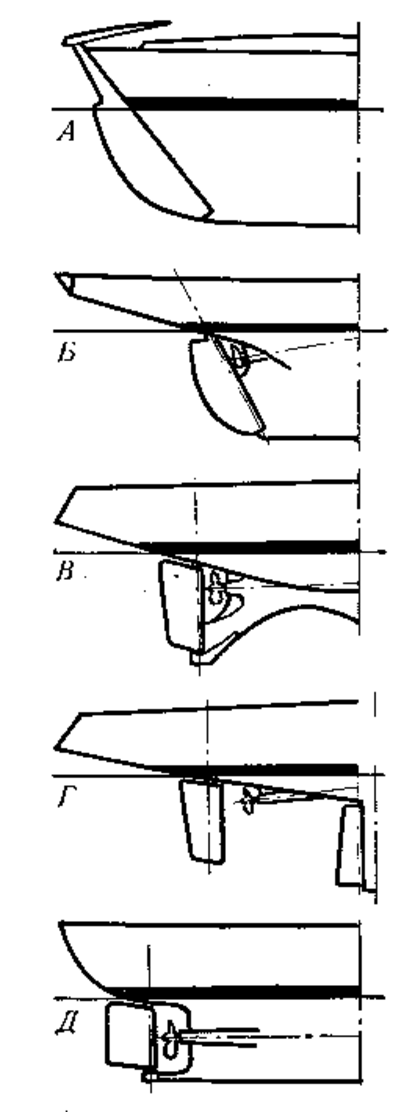
\includegraphics{Postoyannye_ruli}
\par\end{centering}

\protect\caption{\label{fig:30}Основные типы постоянных рулей}


\end{wrapfigure}%


Рули подразделяют на постоянные и подвесные.

Постоянные рули (рис.~\ref{fig:30})
ставят на килевых яхтах и подвешивают к ахтерштевню, плавнику фальшкиля,
а также к специальному плавнику либо кронштейну.

Основные части постоянного руля (рис.~\ref{fig:31}):
перо \--- деревянная или металлическая пластина; баллер \--- стержень, на
котором укреплено перо; румпель \--- рычаг для поворота руля и гельмпорт
\--- труба, через которую проходит верхняя часть баллера. На больших
судах, где силы человека недостаточно, чтобы повернуть руль, вместо
румпеля применяются различные рулевые приводы, позволяющие с помощью
штурвала повернуть руль, не прилагая больших усилий.{\sloppy\par}

Руль подвешивается к ахтерштевню на петлях; нижняя часть баллера \---
пятка опирается на подпятник \--- основательную оковку, прикрепленную к
ахтерштевню, дейдвуду или фальшкилю.

Разновидностью постоянного руля является балансирный руль (рис.~\ref{fig:30},
\emph{г}), консольно, без петель, укрепленный на баллере, причем часть
площади пера расположена впереди оси вращения. Давление набегающей
воды на эту часть пера уменьшает усилие, необходимое для поворота
руля.

Подвесные рули применяют на швертботах и килевых яхтах с обрезной
транцевой кормой.

На швертботах часто встречается подвесной руль с подъемным пером (рис.~\ref{fig:32}),
у которого нет баллера, а перо на горизонтальной оси подвешено в деревянной
или металлической рулевой коробке, в нее и вставлен румпель. Перо
может быть приподнято или совсем поднято из воды сорлинем \--- тросиком,
один конец которого (коренной) закреплен на пере, а другой пропущен
через шкив на коробке или румпеле и может быть закреплен на румпеле
в нужном положении.

На некоторых швертботах (например, класса <<Финн>>) ставят руль, перо
которого составляет с рулевой коробкой одно целое. Обычно такой руль
делается из дерева или фанеры, перо его профилируется, а сам руль
имеет крепление к транцу на петлях, позволяющее легко снимать перо
при подходе к берегу или при вытаскивании швертбота на берег.

\begin{figure}[htbp]
\begin{centering}
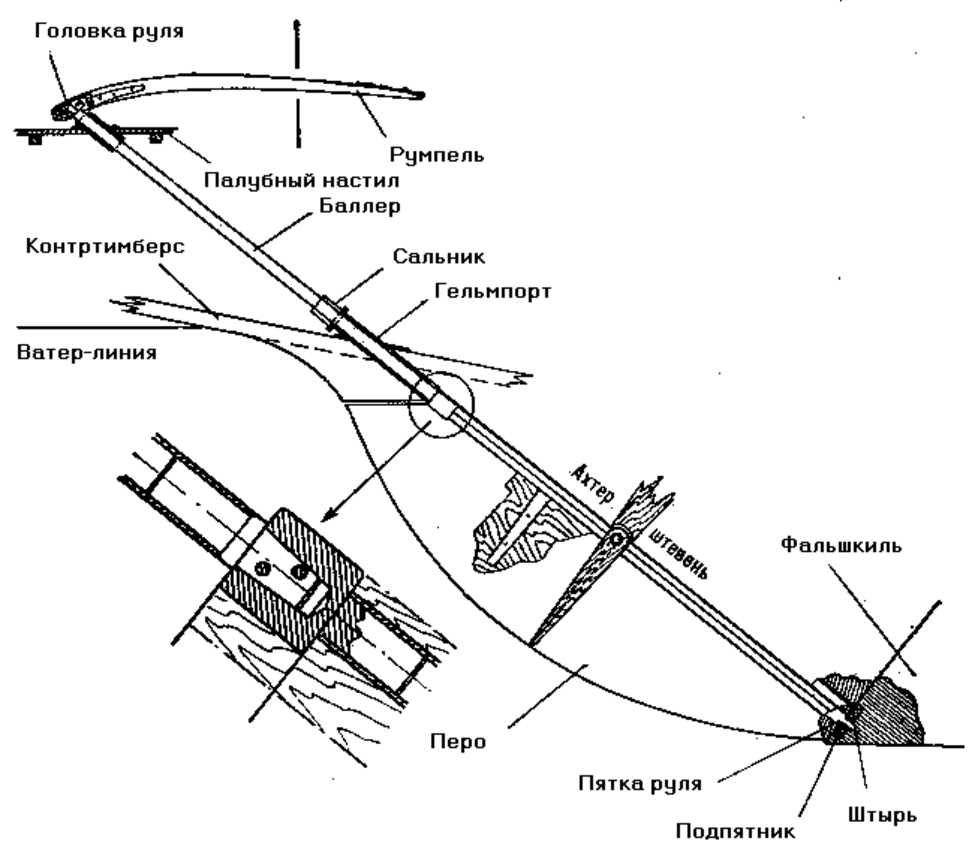
\includegraphics{Rul_kilevoy_yakhty}
\par\end{centering}

\protect\caption{\label{fig:31}Руль килевой яхты и его части}


\end{figure}


\textbf{Швертовое устройство}\index{швертовое устройство} состоит из шверта, швертового колодца
и шверт-талей.

Шверты изготовляют из листового металла (сталь, медные или алюминиевые
сплавы) или дерева. Шверты бывают кинжальные и качающиеся.

\begin{wrapfigure}{I}{0.5\columnwidth}%
\begin{centering}
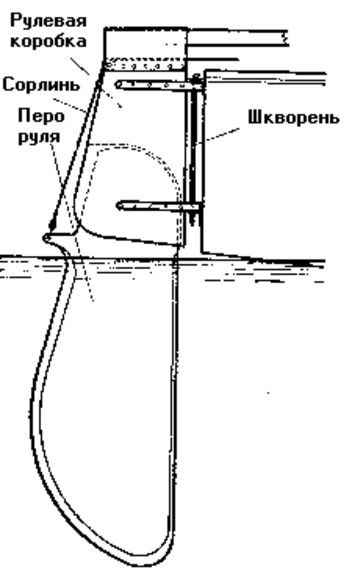
\includegraphics{Rul_shvertbota}
\par\end{centering}

\protect\caption{\label{fig:32}Устройство подвесного руля швертбота}


\end{wrapfigure}

\textbf{Кинжальный шверт}\index{шверт!кинжальный} (рис.~\ref{fig:33},
\emph{а}) вставляется в швертовый колодец, как кинжал в ножны, и передвигается
в нем поступательно. Кинжальные шверты неудобны тем, что при задевании
за мель их заклинивает в колодце.

Кинжальными швертами снабжены швертботы юношеских классов <<Оптимист>>
и <<Кадет>>. Применяют их также на катамаранах.

\textbf{Качающиеся шверты}\index{шверт!качающийся} опускаются поворотом вокруг своей оси,
бывают двух видов \--- секторные и прямые.

\textbf{Секторный шверт}\index{шверт!секторный} (рис.~\ref{fig:33},
\emph{б}) имеет то преимущество, что при опускании его швертовая щель
остается закрытой телом шверта, а за прямым швертом (рис.~\ref{fig:33},
\emph{в}), когда он опущен, остается открытой швертовая щель, создающая
добавочное сопротивление корпуса. С другой стороны, когда секторный
шверт выбран, он сильно выходит за пределы колодца и мешает экипажу.
Поэтому секторные шверты делают главным образом на небольших швертботах
(например, класса <<Финн>>). 


\textbf{Прямой шверт}\index{шверт!прямой} меньше мешает и имеет еще одно достоинство:
когда его подбирают, значительно смещается назад центр бокового сопротивления,
и швертбот можно центровать на ходу.

\begin{wrapfigure}{I}{0.5\columnwidth}%
\begin{centering}
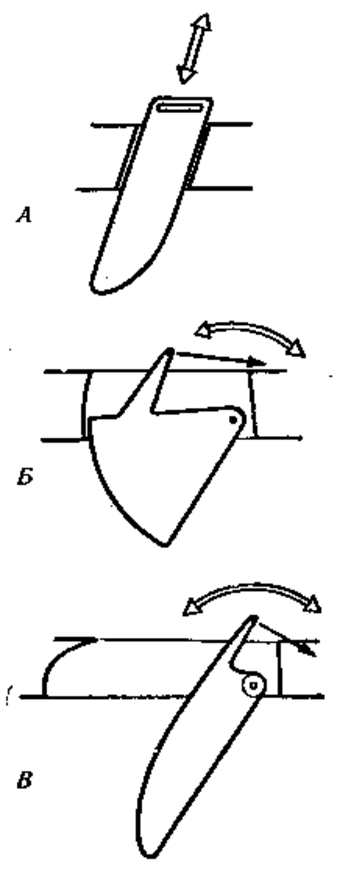
\includegraphics{Tipy_shvertov}
\par\end{centering}

\protect\caption{\label{fig:33}Типы швертов}


\centering{}\small А \--- кинжальный; Б \--- качающийся секторный, В \--- качающийся мечевидный
\end{wrapfigure}

Для усиления эффекта перемещения центра бокового сопротивления применяют
узкие, длинные, так называемые мечевидные шверты (рис.~\ref{fig:33},
\emph{в}). Ими снабжено большинство современных швертботов. Часто
для уменьшения сопротивления шверты профилируют, то есть в поперечном
сечении придают им профиль симметричного крыла самолета. Они дают
некоторый выигрыш в лавировочных качествах за счет меньшего сопротивления.
Чтобы уменьшить сопротивление широкой щели на выходе швертового колодца
в днище, щель для профилированного шверта снабжают сальниками из листовой
резины: когда шверт выбран, сальники смыкаются и закрывают щель.

Шверт вращается вокруг болта, под головку и гайку которого положены
большие шайбы с кожаными или резиновыми прокладками для предохранения
от подтекания.

\textbf{Швертовый колодец}\index{швертовый колодец} (см. рис.~\ref{fig:26})
имеет основание из двух досок, обычно дубовых, притянутых к килю болтами.
Поверх основания набраны стенки из более тонких досок. Сзади и спереди
колодец ограничен вертикальными стойками, к которым приклепываются
основание и стенки. По верхнему обрезу колодца положен планширь. На
него ложится резиновый буфер, надетый на болт рычага шверта и предохраняющий
колодец от разрушения при ударе болта о планширь. Поперечную устойчивость
колодца обеспечивает крепление его к флорам кницами или \textbf{шпонками}\index{шпонка}
\--- вертикально поставленными поперечными досками. Часто колодец укрепляют
специальной поперечиной, связывающей колодец (через планширь) с карлингсами
и палубным настилом. На пластмассовых швертботах колодцы проще по
конструкции \--- тонкостенный ящик, приформованный к усиленной обшивке
днища. 

%--------------------------------------------------------------------------
%
%                                   Паруса
%
%--------------------------------------------------------------------------

\section{Паруса}

Паруса \--- это главная часть вооружения яхты, её движитель. Шьют их
из отдельных полос парусины \--- полотнищ. Швы, соединяющие полотнища,
располагаются под прямым углом к задней кромке \--- \textbf{шкаторине}\index{шкаторина}
\--- паруса. Треугольный парус имеет переднюю, заднюю и нижнюю шкаторины,
независимо от того, грот это, кливер, стаксель или иной парус. Четырехугольный
парус имеет еще верхнюю шкаторину.

\begin{figure}[htbp]
\begin{centering}
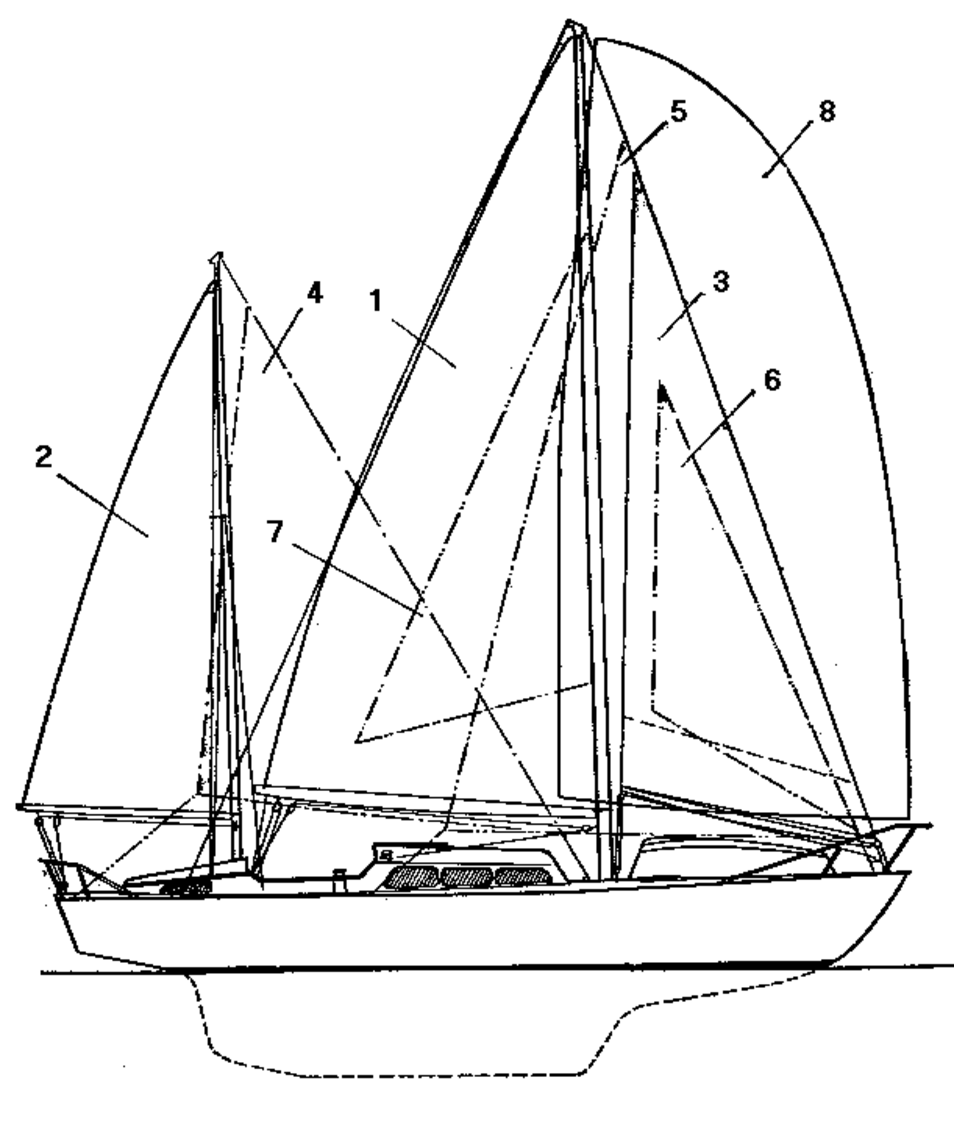
\includegraphics{Parusnost_bermudskogo_kecha}
\par\end{centering}

\protect\caption{\label{fig:34}Парусность
бермудского кэча}


\centering{}\small 1 \--- грот; 2 \--- бизань; 3 \--- стаксель; 4 \--- бизань-стаксель (апсель);
5 \--- генуэзские стаксель; 6 \--- штормовой стаксель; 7 \--- трисель; 8 \--- спинакер
\end{figure}


На рис.~\ref{fig:35} и \ref{fig:36} показаны основные части треугольного и четырехугольного гротов.

У треугольного паруса различают \textbf{фаловый}\index{угол паруса!фаловый}, \textbf{шкотовый}\index{угол паруса!шкотовый}
и \textbf{галсовый}\index{угол паруса!галсовый} углы. У четырехугольного грота, имеющего два верхних
угла, передний угол называется \textbf{верхним галсовым}\index{угол паруса!верхний галсовый}, задний \---
\textbf{нок-бензельным}\index{угол паруса!нок-бензельный}. Передний нижний угол носит название \textbf{нижнего галсового}\index{угол паруса!нижний галсовый}, задний, как и у треугольного паруса, \--- \textbf{шкотового}\index{угол паруса!шкотовый}
угла.

Для прочности по шкаторинам парус обшивается \textbf{ликтросом}\index{ликтрос} \---
специальным тросом отлогого спуска.

Углы паруса и другие места, подвергающиеся большим нагрузкам, усиливают
боутами \--- накладками из парусины соответствующей формы. Ликтросы и боуты
составляют как бы раму, которая препятствует излишнему растяжению
паруса. Ликовке\footnote{Неправильно называть ликтрос ликовкой, как это часто делают. Ликтрос
пришивают к парусу. Этот процесс и называется ликовкой} обычно подвергаются передняя, нижняя и верхняя шкаторины парусов,
задняя же ликуется только частично (у углов). У передних парусов (стаксель,
кливер) чаще всего ликуются только передняя шкаторина и углы, у спинакера
\--- все шкаторины очень тонким стальным тросом. Передняя шкаторина передних
парусов иногда ликуется стальным тросом. Штормовые и некоторые дополнительные
паруса, о которых речь пойдет дальше, ликуются по всем шкаторинам. 

Задняя шкаторина грота всегда имеет больший или меньший выгиб наружу
\--- горб, который не может стоять без поддержки тонких деревянных дощечек
\--- \textbf{лат}\index{латы}, вставляющихся в соответствующие карманы. Латы должны
входить в карманы плотно, но без излишнего усилия. Карман делают длиннее
латы на 2\==4 см. Латы могут быть короткими и сквозными. Короткие латы
делают тоньше у внутреннего и толще у наружного конца; самое тонкое
место у сквозных лат \--- примерно на одной трети длины от внутреннего
конца, чуть толще они у внутреннего и еще толще у наружного конца.

Латы делают из упругого и нехрупкого дерева (ясень, сосна, орех и
др.) или из слоистых пластиков типа текстолита. Чтобы они не упирались
во внутренний торец кармана и надежно поддерживали заднюю шкаторину,
внутрь кармана обычно вшивают резиновую полоску, которая оттягивает
лату наружу.

\begin{figure}[htbp]
\begin{centering}
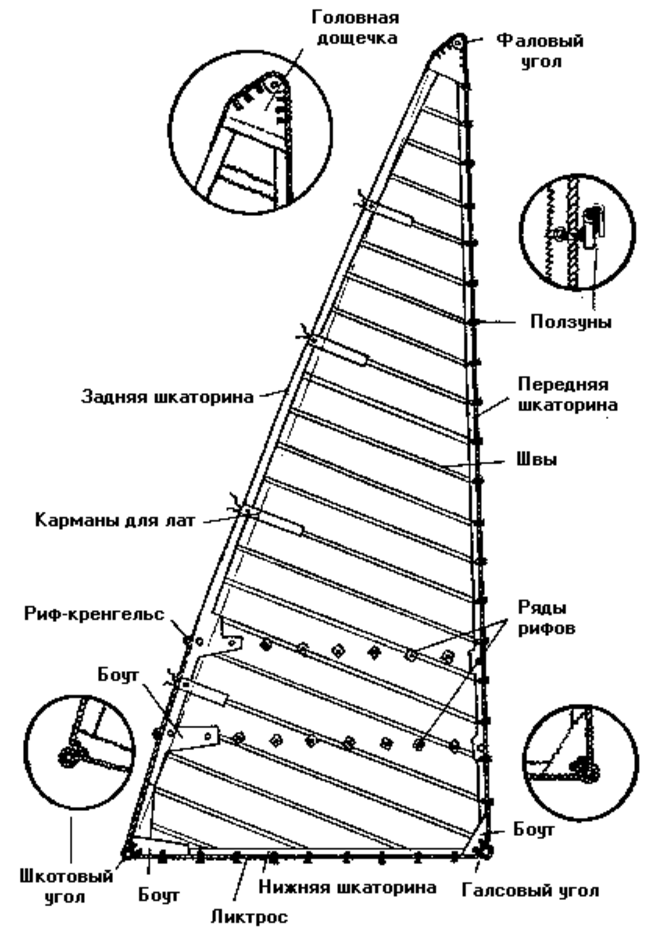
\includegraphics{Bermudskij_grot}
\par\end{centering}

\protect\caption{\label{fig:35}Бермудский грот и его части}
\end{figure}


Сквозными латами можно регулировать в небольших пределах величину
и положение <<пуза>> паруса.

Для предохранения задней шкаторины от растяжения внутрь её кромки
пропускают тонкую крепкую снасть \--- булинь, который можно подтянуть
или ослабить \--- выбрать или потравить, в зависимости от условий работы
паруса. Булинь одним концом заделывается около фалового (нокбензельного)
угла; другой его конец выходит около шкотового угла. У генуэзских
стакселей иногда ставят булинь по нижней шкаторине, чтобы регулировать
<<пузо>> паруса в нижней его части. Поперек паруса, параллельно нижней
шкаторине, проделаны ряды \textbf{люверсов}\index{люверсы} \--- окантованных отверстий,
через которые при уменьшении площади паруса \--- \textbf{взятии рифов}\index{рифы!взятие}
\--- пропускаются тонкие снасти, называемые \textbf{риф\-/штертами}\index{риф-штерты}. Эти
ряды люверсов усилены полосками парусины \--- \textbf{риф\-/бантами}\index{риф-банты}. В настоящее
время сплошные риф\-/банты применяют редко, чаще \--- в виде ромбовидных
накладок около каждого из люверсов. Обычно их делают два-три ряда,
почему и говорят свзять два (один, три) ряда рифов>>, то есть уменьшить
парус настолько, чтобы притянуть к гику второй (первый, третий) ряд
риф-бантов. У концов риф-бантов делают \textbf{риф\-/кренгельсы}\index{риф-кренгельсы} \--- веревочные
петли с заделанными внутрь металлическими кольцами \--- \textbf{коушами}\index{коуши}.
В передний риф-кренгельс продергивается \textbf{штык\-/болт}\index{штык-болт}, а в задний \--- \textbf{риф-шкентель}\index{риф-шкентель} \--- снасти,
которыми парус при рифлении притягивают к гику. Кренгельсы также заделываются
по углам парусов.

\begin{figure}[htbp]
\begin{centering}
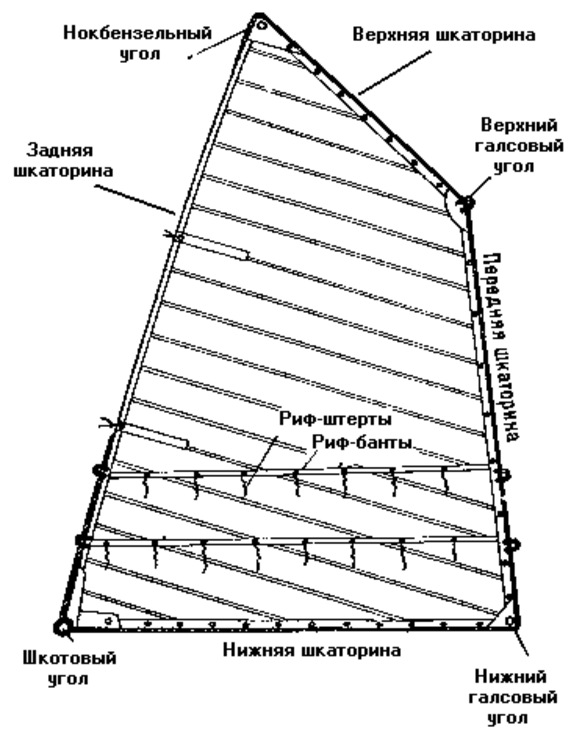
\includegraphics{Gafelnyj_grot}
\par\end{centering}

\protect\caption{\label{fig:36}Гафельный
грот и его части}
\end{figure}


Чтобы увеличить ширину треугольного грота в верхней части, к боуту
фалового угла крепят или вставляют внутрь небольшую головную (фаловую)
дощечку, ширина которой ограничена правилами обмера. Грот крепится
к гику своим галсовым углом обычно за соответствующую оковку у пятки
(внутреннего конца) гика с помощью такелажной скобы или болта. Нижняя
шкаторина грота растягивается вдоль гика грота-шкотом \--- специальной
снастью, заделанной в кренгельс шкотового угла. Передняя и нижняя
шкаторины крепятся к гику или мачте одним из следующих способов (рис.~\ref{fig:37}):

\begin{itemize}
\item шкаторина продергивается внутрь круглого паза с губками (лик-паза)
на гике или мачте (рис.~\ref{fig:37}, \emph{а} и \emph{е});

\item через люверсы по шкаторинам пришиваются ползуны,которые
либо входят внутрь охватывающего их рельса, либо сами охватывают рельс
(рис.~\ref{fig:37}, \emph{б, е, г} и \emph{д});

\item шнуровка, продернутая через люверсы по шкаторинам и охватывающая
гик (или гафель); на гафельном гроте таким образом крепится передняя
шкаторина \--- тогда шнуровку называют \textbf{слаблинем}\index{слаблинь};

\item охватывающие мачту кольца, которые прикрепляются к передней шкаторине
гафельного грота; эти кольца называют \textbf{сегарсами}\index{сегарсы}. Чтобы при
постановке грота сегарсы не заедали, спереди их соединяют тонким тросом;
расстояние между ними должно быть равно расстоянию между люверсами
на передней шкаторине.

\end{itemize}

Передние шкаторины передних парусов соединяются со штагами карабинами
(их привязывают к передней шкаторине и надевают на штаг) или такелажными
скобами\-/мочками (см. рис.~\ref{fig:51}).

%--------------------------------------------------------------------------
%
%                        Рангоут и стоячий такелаж
%
%--------------------------------------------------------------------------

\section{Рангоут и стоячий такелаж}

\begin{figure}[htbp]
\centering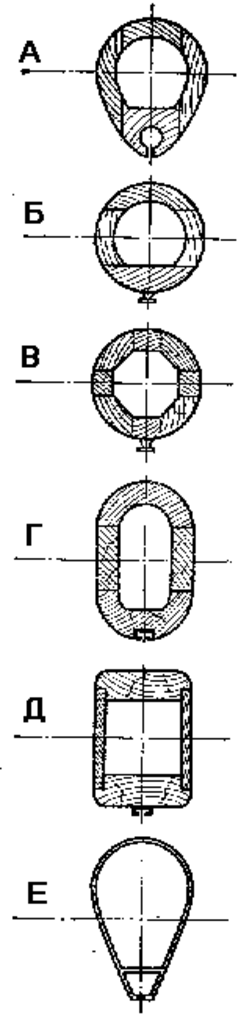
\includegraphics{Sechenija_rangouta}
\caption{Сечения рангоута}
\label{fig:37}
\centering\small
А \--- каплевидная деревянная мачта с лик-пазом; Б и В \--- круглые мачты
с рельсами под наружные ползуны; Г и Д \--- мачты с рельсам под внутренние
ползуны, Е \--- металлическая мачта с лик-пазом 
\end{figure}


Главной частью рангоута является \textbf{мачта}\index{мачта}. Мачты, как и другие
части рангоута, могут быть сплошного сечения и пустотелые. При равной
прочности пустотелый рангоут значительно легче сплошного и поэтому
предпочтительнее.

На современных яхтах широко распространен металлический рангоут из
легких сплавов; на больших яхтах встречается и стальной. Металлический
рангоут легче деревянного, не меняет веса при изменениях влажности,
не гниет.

На рис.~\ref{fig:37}
показаны типовые сечения деревянного и металлического рангоута.

Верхний конец мачты называется \textbf{топом}\index{мачта!топ}, нижний \--- \textbf{шпором}\index{мача!шпор}.
Шпор мачты проходит в \textbf{пяртнерс}\index{пятнерс} и опирается в \textbf{степс}\index{степс} \--- деревянную
или металлическую подушку, укрепленную на киле яхты. Чтобы мачта не
болталась в пяртнерсе, её расклинивают деревянными клиньями, а чтобы
в щели не протекала вода, покрывают пяртнерс чехлом в виде рукава
\--- \textbf{брюканцем}\index{брюканец}, который охватывает мачту верхним обрезом, а
нижним плотно надевается на оковку, окружающую пяртнерс.

На многих современных крейсерско-гоночных яхтах степс мачты устанавливают
прямо на палубе. Благодаря этому мачта не занимает места в каюте,
а поскольку она не опирается на киль, то обшивка в районе степса не
испытывает повышенной нагрузки. В результате деревянная яхта меньше
течет.

Мачта бывает и складной, то есть может быть положена вокруг оси, закрепленной
в \textbf{пасынках}\index{пасынки}. Пасынки либо проходят сквозь пяртнерс и своим
шпором упираются в степс (как и обычная мачта), либо крепятся прямо
на палубе. Иногда их называют \textbf{стандерсами}\index{стандерсы}. Складные мачты очень удобны
для речных и озерных плавании, когда приходится часто проходить под
низкими мостами, проводами и другими препятствиями. Убрать и поставить
снова такую мачту для хороших матросов дело 10\--15 минут даже на яхте
парусностью 40\--60~м$^2$.

Самое толстое место у мачты находится примерно на середине высоты
переднего треугольника. К шпору и вершине переднего парусного треугольника
мачта тоньше на 10\--15\%, а к топу \--- на 40\--50\%. Естественно, что при
топовом стакселе, когда вершина переднего треугольника совпадает с
топом мачты, максимальный диаметр её придется на середину, а диаметры
у шпора и топа будут одинаковы \--- 85\--90\% максимального. Металлические
мачты при вооружении с топовым стакселем делают просто цилиндрическими.

\textbf{Стоячий такелаж}\index{такелаж!стоячий} состоит из \textbf{вант}\index{ванта}, Поддерживающих
мачту от изгиба к бортам, \textbf{штагов}\index{штаг}, поддерживающих её от изгиба
назад, и \textbf{бакштагов}\index{бакштаг}, поддерживающих от изгиба вперед. На швертботах-кэтах,
например класса <<Финн>> и <<ОК>>, мачта не имеет стоячего такелажа и
под действием ветра на паруса свободно прогибается.

На бермудских мачтах верхние концы стоячего такелажа крепят к оковкам
особой формы, охватывающим мачту и закрепленным на ней болтами или
шурупами.

На гафельной яхте верхние концы частей стоячего такелажа надеваются
на мачту заделанными на них петлями \--- \textbf{огонами}\index{огон}. Огоны опираются
на \textbf{чиксы}\index{чикса} \--- деревянные или металлические заплечики, предохраняющие
их от сползания.

Если на яхте две пары вант, то верхние называют топ-вантами, а нижние \---
основными. Чтобы увеличить угол между мачтой и вантой, топ-ванты часто
распирают краспицами (рис.~\ref{fig:38}).

Если вант несколько пар и все они идут нижними концами на палубу,
то те, что идут на самый топ мачты, называют \textbf{топ-вантами}\index{топ-ванта}\footnote{Если мачта имеет стеньгу, то ванты, идущие с топа стеньги, называют
стень-вантами}. Дальше вниз по порядку расположены: верхние ванты, средние и нижние.

Сколько бы ни было пар вант, самые нижние, идущие прямо на палубу,
без краспиц, называют основными. Топ-ванты всегда проводят в плоскости
мачты, а основные \--- слегка к корме. Когда основных вант две пары,
одну из них проводят несколько впереди мачты.

Если краспиц больше одной пары, их называют верхние, средние, нижние;
если больше трех пар, \--- по номерам, начиная снизу (первые краспицы,
вторые, третьи и т.\,д.).

На гоночных швертботах часто обходятся одной парой вант, проведенных
позади мачты и распираемых краспицами так, чтобы они прогибали мачту
вперед. Таким образом, при усилении ветра уплощается грот.

На бермудских мачтах часто делают \textbf{ромбо-ванты}\index{ромбо-ванта}, они идут на
мачту с самого топа через верхние краспицы. На рис.~\ref{fig:38} показаны различные
способы проводки вант.

\textbf{Штаг}\index{штаг}, идущий от вершины переднего парусного треугольника
и поддерживающий стаксель, называют \textbf{основным}\index{штаг!основной}, а если нет
других, то просто штагом. Если штагов несколько, то штаг, идущий с
топа мачты, называют \textbf{топ-штагом}\index{штаг!топ-штаг}\footnote{На мачтах со стеньгой штаг, поддерживающий топ стеньги, называется
стень-штагом. Применение этого термина к современным бермудским мачтам,
как иногда можно слышать, не имеет смысла.}, штаг, на котором ставится кливер, \textbf{кливер-леером}\index{кливер-леер}.

\begin{figure}[htbp]
	\begin{minipage}[b]{0.49\textwidth}
		\centering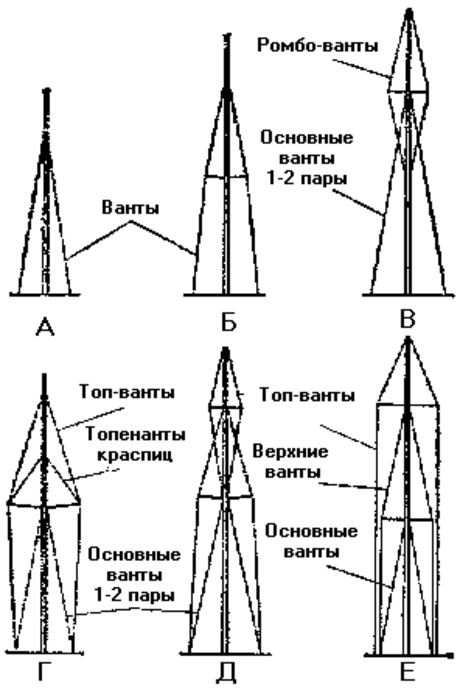
\includegraphics{38_Provodka_vant}
		\caption{Проводка вант}
		\label{fig:38}
	\end{minipage}
	\hfil\hfil%
	\begin{minipage}[b]{0.49\textwidth}
		\centering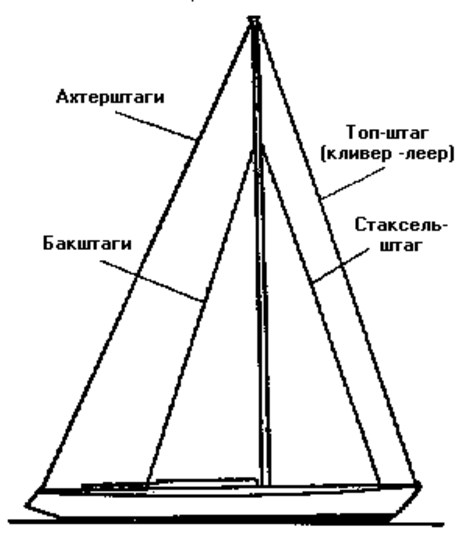
\includegraphics{Provodka_shtagov}
		\caption{Проводка штагов}
		\label{fig:39}
	\end{minipage}
	\par
	\smallskip
	\begin{minipage}[b]{0.49\textwidth}
		\centering\small
		А \--- маленькие швертботы ( класс <<Кадет>>); Б \--- гоночные швертботы (классы М, <<Летучий голландец>>); В \--- крейсерские швертботы в малые килевые яхты с низким передним треугольником (класс <<Фолькбот>>); Г \--- яхты с топовыми стакселями; Д \--- средние килевые яхты; Е \--- крупные яхты
	\end{minipage}
	\hfil\hfil%
	\begin{minipage}[b]{0.49\textwidth}
		\centering\small
		
	\end{minipage}
\end{figure}

У яхт с бермудским вооружением топ мачты в большинстве случаев поддерживается
еще одним или двумя \textbf{ахтер\-/штагами}\index{ахтер-штаг}, идущими на корму судна
(рис.~\ref{fig:39}).

\textbf{Бакштаги}\index{бакштаг} идут на палубу судна к бортам от того места на мачте,
где крепится основной штаг. Крепят бакштаги таким образом, чтобы их
можно было отдавать и выбирать при смене галса. Для этого нижние концы
бакштагов снабжаются талями или ползунами, которые перемещаются по
закрепленным на палубе рельсам или туго натянутым стальным тросам
\--- \textbf{шпрюйтам}\index{шпрюйт}. На современных яхтах широкое распространение
получили быстродействующие рычажные натяжки, или лебедки, облегчающие
работу команды и ускоряющие отдачу и закладывание бакштагов (см. рис.~\ref{fig:51}).
Такими натяжками иногда снабжают и задние основные ванты \--- тогда подветренная
ванта ослабляется и не режет грот.

Если бакштагов две пары, то те, что проведены выше стаксель-штага,
называют \textbf{фордунами}\index{бакштаг!фордун}; а бакштаги, проведенные ниже основных,
\--- \textbf{нижними}\index{бакштаг!нижний}.

На многих современных гоночных яхтах стоячий такелаж не столько поддерживает
мачту от изгиба, сколько ограничивает этот изгиб. Речь идет о так
называемом гибком рангоуте, стоячий такелаж которого проводится и
регулируется так, чтобы мачта имела возможность прогнуться под действием
ветра. Основная роль такого прогиба \--- регулирование <<пуза>> паруса.
Чем сильнее ветер, тем, вообще говоря, меньше должно быть <<пузо>>.
А так как прогиб мачты увеличивается с усилением ветра, то величина
<<пуза>> паруса регулируется как бы автоматически по силе ветра.

Гибкий рангоут сейчас применяется почти на всех гоночных швертботах
и на многих яхтах, в том числе и на крейсерско-гоночных.

У двухмачтовой яхты к названиям частей стоячего такелажа прибавляется
название мачты (например, бизань-ванты, основные грота-ванты, грота-штаг,
фор-топ-штаг, бизань-бакштаг и т.\,д.). Двухмачтовые яхты часто имеют
еще \textbf{штаг-карнаки}\index{штаг-карнак}, соединяющие топы мачт.

\begin{figure}[htbp]
\begin{centering}
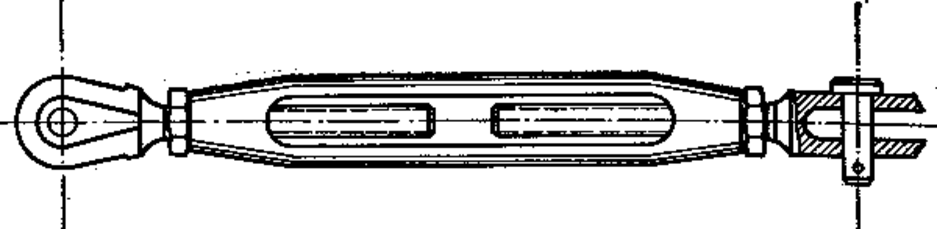
\includegraphics{Vintovoj_talrep}
\par\end{centering}

\protect\caption{\label{fig:40}Винтовой талреп}


\bigskip{}


\begin{centering}
\begin{tabular}{|c|c|c|c|c|c|c|}
\hline 
Диаметр троса, мм & до 2,0 & 2,5\-- 3 & 3,2\-- 4,2 & 4,5\-- 5,2 & 5,5\-- 6,2 & 6,5\-- 8,0\tabularnewline
\hline 
Резьба талрепа & М5 & М6 & М8 & М10 & М12 & М14\tabularnewline
\hline 
\end{tabular}
\par\end{centering}

%\bigskip{}

\end{figure}

\begin{table}
\protect\caption{Рекомендуемые размеры талрепов}


\end{table}

У иола и кэча штаги бизань-мачты мешали бы свободному переходу грота
с борта на борт, поэтому передние основные бизань-ванты выносят настолько
вперед, что они заменяют штаги.

Ванты и штаги крепятся к корпусу на соответствующих оковках \--- \textbf{вант\-/путенсах}\index{путенс!вант-путенс}
и \textbf{штаг-путенсах}\index{путенс!штаг-путенс}, надежно закрепленных на самом корпусе яхты.
Натяжение вант осуществляется \textbf{талрепами}\index{талреп} \--- винтовыми стяжками (рис.~\ref{fig:40}).

\textbf{Гик}\index{гик} \--- горизонтальное рангоутное дерево, к которому одним из способов
(рис.~\ref{fig:37})
крепится нижняя шкаторина грота (бизани, фока). Гик грота называется
\textbf{грота\-/гик}\index{гик!грота-гик}\footnote{На одномачтовой яхте просто гик.},
гик бизани \--- \textbf{бизань\-/гик}\index{гик!бизань-гик}, гик фока \--- \textbf{фока\-/гик}\index{гик!фока-гик}. Конец гика, упирающийся в мачту, называется \textbf{пяткой}\index{пятка}, противоположный
конец \--- \textbf{ноком}\index{нок}. Пятка гика имеет оковку, которая входит в
вертлюг, позволяющий гику поворачиваться в стороны и вверх. Вертлюг
часто делают передвижным вверх по рельсу (особенно на гоночных яхтах),
чтобы иметь возможность добрать парус, не трогая фала, при помощи
\textbf{галс\-/оттяжки}\index{галс-оттяжка} (рис.~\ref{fig:41}).

Если рифы берут накручивая парус на гик, то для вращения гика применяют
машинку \--- патент-риф, смонтированную с оковкой пятки.

На \textbf{ноке гика} укрепляются оковки для присоединения \textbf{гика-топенантов}\index{гика-топенант}
\--- снастей бегучего такелажа, поддерживающих нок. Шкотовый угол крепят
к ползунку, передвигающемуся по рельсу. Ползун имеет шкив для грота-шкота,
которым растягивается нижняя шкаторина гика. Грота-шкот крепится на
утку или стопор на гике или вяжется вокруг гика.

\begin{figure}[htbp]
	\begin{minipage}[b]{0.49\textwidth}
		\centering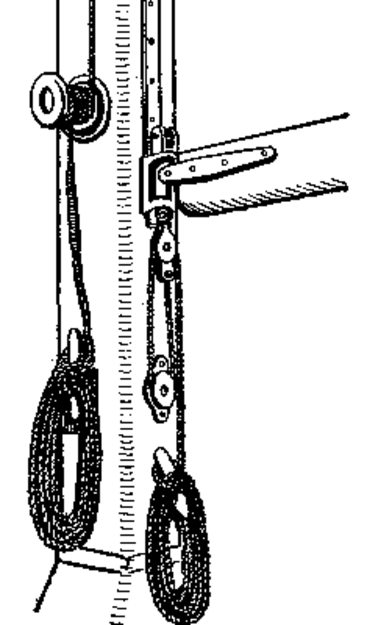
\includegraphics[scale=0.9]{Peredvizhnoj_vertljug_gika}
		\caption{Передвижной вертлюг гика}
		\label{fig:41}
	\end{minipage}
	\hfil\hfil%
	\begin{minipage}[b]{0.49\textwidth}
		\centering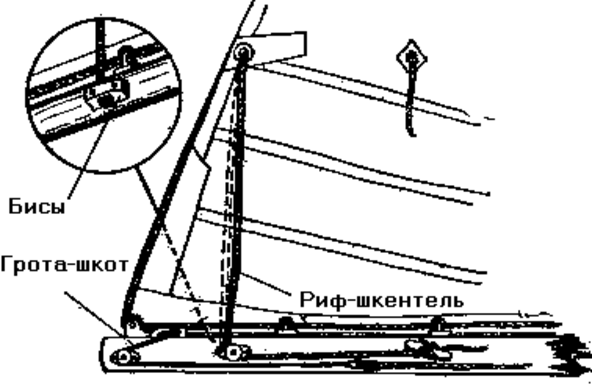
\includegraphics[scale=0.85]{Nok_gika}
		\caption{Нок гика}
		\label{fig:42}
	\end{minipage}
\end{figure}

На крупных яхтах риф-шкентели проводят через \textbf{бисы}\index{бис} \--- деревянные
планки или оковки со шкивами (рис.~\ref{fig:42}).
На малых яхтах устройство много проще.

Блоки \textbf{гика-шкотов}\index{гика-шкот}, то есть снастей, посредством которых управляют
гиком, подвешивают к гику на стропах из проволочного троса или оковках,
прикрепленных к гику болтами. Если гик имеет патент-рифы, то их подвешивают
на открытых бугелях, снабженных роликами. При взятии рифов гик с наматываемым
на него парусом вращается внутри такого бугеля. Ноковую оковку гика
с патент-рифом делают вращающейся вокруг оси гика; к этой оковке крепят
топенанты и, если нужно, подвешивают блоки гика-шкотов, обходясь таким
образом без бугелей.

Гики бывают круглого, овального или прямоугольного сечения. Самая
большая толщина у гика примерно в середине или ближе к пятке; к концам
он суживается процентов на 20\--30. Гики под патент-риф делают круглыми
и равного диаметра по всей длине.

\begin{wrapfigure}{O}{0.5\columnwidth}%
\begin{centering}
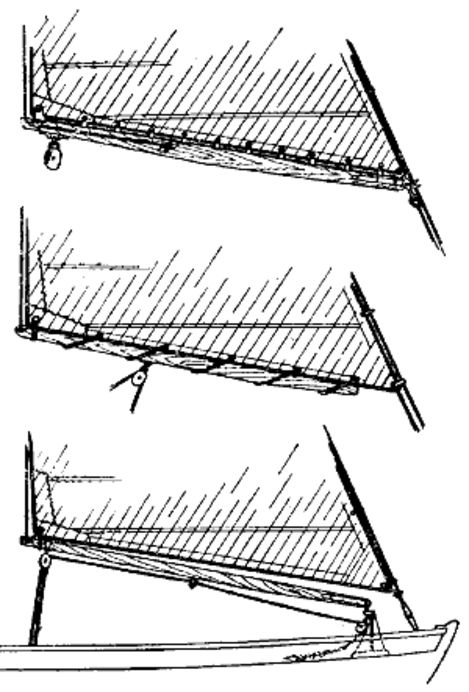
\includegraphics{Rejki_stakselej}
\par\end{centering}

\protect\caption{\label{fig:43}Рейки стакселей}


\end{wrapfigure}%


\textbf{Гафель}\index{гафель}, как и гик, имеет \textbf{нок}\index{нок} и \textbf{пятку}\index{пятка}. Пятка гафеля имеет
\textbf{усы}\index{усы}, схватывающие мачту. Усы могут быть неподвижными или
вертлюжными: неподвижные чаще всего делают из дерева (дуба или ясеня),
а вертлюжные \--- из металла. Поверхность усов, обращенную к мачте, обшивают
кожей, а место на мачте, где они ходят, \--- тонкой листовой медью или
латунью, предохраняя её таким образом от износа. Чтобы усы не соскочили
с мачты, концы их соединяют тонким стальным тросиком \--- \textbf{бейфутом}\index{бейфут}.
Одним из концов бейфут крепится к усам тонкой пеньковой снастью такой
крепости, чтобы при падении гафеля она рвалась, предохраняя усы от
поломки. На бейфут надевают деревянные шарики \--- \textbf{раксклоты}\index{раксклот},
чтобы он легче ходил по мачте и не царапал её.

Когда паруса велики по сравнению с корпусом и не умещаются на нем,
с носа выдвигается (выстреливается) горизонтальное рангоутное дерево
\--- \textbf{бушптрит}\index{бушптрит}. Наружный конец его называют \textbf{ноком}\index{нок}, а внутренний
\--- \textbf{шпором}\index{шпор}, как у мачты.

Бушприт имеет следующий стоячий такелаж: \textbf{ватер-штаг}\index{ватер-штаг}, соединяющий его
нок с форштевнем, и \textbf{ватер-бакштаги}\index{ватер-бакштаг}, соединяющие нок с бортами судна.
\textbf{Ватер-штаг} отводится от бушприта краспицей, которая здесь носит название
\textbf{мартин-гика}, а \textbf{ватер-бакштаги} \--- краспицами, именуемыми
\textbf{блинда-гафелями}\index{блинда-гафель}.

Кроме перечисленных частей рангоута на яхтах применяют \textbf{спинакер-гики}\index{спинакер-гик}
(для дополнительных парусов \textbf{спинакеров}), а также рейки стакселей и
кливеров (рис.~\ref{fig:43}).
Рейки стакселей иногда называют \textbf{стаксель-гиками}\index{стаксель-гик}.

%--------------------------------------------------------------------------
%
%                             Бегучий такелаж
%
%--------------------------------------------------------------------------

\section{Бегучий такелаж}

\textbf{Бегучий такелаж}\index{такелаж!бегучий} состоит из фалов. шкотов, галсов, топенантов и брасов.
\textbf{Фалы}\index{фал} служат для подъема парусов (или частей рангоута). Конец
фала (как и любой другой снасти бегучего такелажа), закрепленный за
поднимаемый парус или рангоутное дерево, называется \textbf{коренным
концом}\index{конец!коренной}. Другой конец, за который тянут, называется \textbf{ходовым}\index{конец!ходовой}.
Названия фалов, которыми поднимают треугольные паруса (бермудские
паруса, стаксели, кливеры, топсели и др.), складываются таким образом:
к слову <<фал>> прибавляют название соответствующего паруса, например
грота-фал, бизань-фал, стаксель-фал, кливер-фал и т.\,д.

Гафельный парус поднимают двумя фалами. Пятка гафеля поднимается \textbf{гарделью}\index{гардель}, а нок \--- \textbf{дирик-фалом}\index{дирик-фал}.

Фалы имеют \textbf{тали}\index{таль}, увеличивающие силу подъема приспособления
из блоков и тросов.

\begin{figure}[htbp]
\begin{centering}
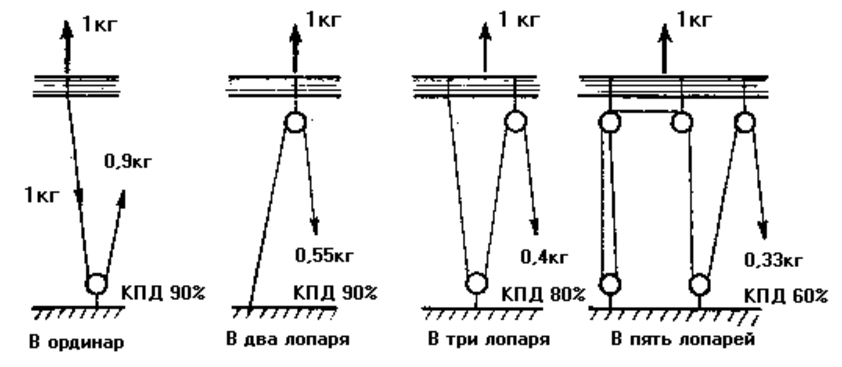
\includegraphics{Provodka_gika-shkotov}
\par\end{centering}

\protect\caption{\label{fig:44}Некоторые способы проводки гика-шкотов}


\end{figure}


\textbf{Блоки}\index{блок} служат для облегчения работы с бегучим такелажем и
изменения направления тяги. Неподвижный блок не дает выигрыша в силе
и служит лишь для изменения её направления. Подвижной блок дает выигрыш
в силе примерно вдвое, но для перемещения груза требует вдвое больше
снасти, чем потребовалось бы без блока. Для определения выигрыша в
силе, который дают тали считают, сколько снастей держит груз. Сколько
таких снастей \--- \textbf{лопарей}\index{лопарь}, таков примерно и выигрыш в силе. Различные
виды талей показаны на рис.~\ref{fig:44}.
Сколько лопарей в талях, во столько раз длиннее надо взять конец для
образования талей.

Блоки бывают самых разных типов. Наиболее распространены пластмассовые
окованные блоки (рис.~\ref{fig:45}),
которые состоят из шкива \--- диска с канавкой на ободе, по которому катится
снасть, нагеля \--- оси шкива, оковки с отверстием для оси и щек, предохраняющих
снасть от трения об оковку и направляющих её по шкиву.

\begin{figure}[htbp]
\begin{centering}
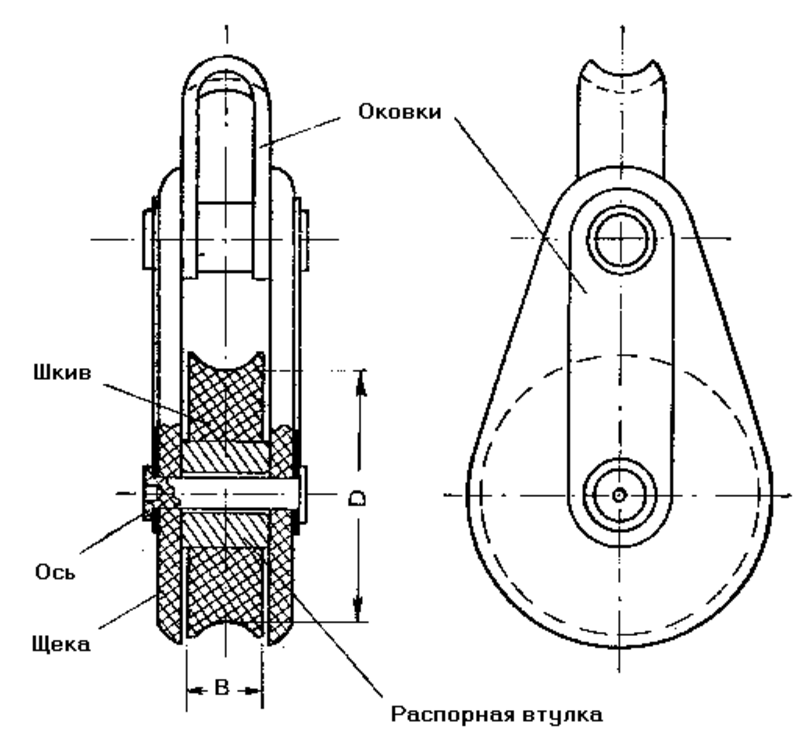
\includegraphics{Platmassovyj_blok}
\par\end{centering}

\protect\caption{\label{fig:45}Пластмассовый блок и его части}


\bigskip{}


\begin{centering}
\begin{tabular}{|l|r|r|r|r|}
\hline 
Наибольший размер троса, мм & 7 & 10 & 13 & 16\tabularnewline
\hline 
Минимальный диаметр шкива D, мм & 30 & 40 & 55 & 65\tabularnewline
\hline 
Минимальная ширина шкива, мм & 10 & 14 & 18 & 22\tabularnewline
\hline 
Максимальная нагрузка на блок, кг & 80 & 100 & 200 & 300\tabularnewline
\hline 
\end{tabular}
\par\end{centering}

\bigskip{}


\centering{}Рекомендуемые размеры блоков
\end{figure}


Для облегчения работы делают так называемые патентованные блоки, у
которых шкивы вращаются на роликах, катающихся между шкивом и нагелем.

Мы говорили, что выигрыш в силе талей примерно равен числу лопарей.
Трение шкива по оси и о щеки, трение троса, его жесткость существенно
увеличивают потери силы.

\begin{wrapfigure}{O}{0.5\columnwidth}%
\begin{centering}
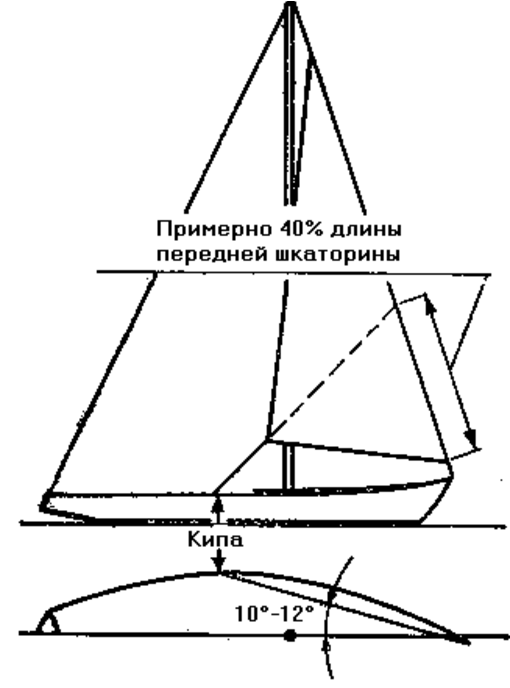
\includegraphics{Provodka_staksel-shkotov}
\par\end{centering}

\protect\caption{\label{fig:46}Проводка стаксель-шкотов}

\end{wrapfigure}%


Коэффициент полезного действия блока (к. п. д.) тем меньше, чем больше
трение шкива по оси и о щеки, больше перегиб троса и трение самого
троса. При нормальной конструкции и размерах блока его к. п. д. составляет
около 90\%; значит, сила на ходовом конце на 10\% больше, чем на коренном.
Если тали сложной конструкции, то потери довольно велики: в частности,
на талях в три лопаря (рис.~\ref{fig:44})
на ходовом конце надо прилагать силу не 0,33~кг, а примерно 0,41~кг,
а при пяти лопарях \--- не 0,2~кг, а 0,34~кг, т.\,е. на 70\% больше теоретической
силы.

При прочих равных условиях к.\,п.\,д. блока тем больше, чем больше отношение
диаметра шкива к диаметру нагеля и диаметру троса. Поэтому надо, чтобы
относительные диаметры блоков были достаточно велики. Практика показала,
что диаметр шкива (по канавке для троса) не должен быть меньше четырех-пяти
диаметров троса, а толщина шкива \--- не менее 1,4\--1,5 диаметра троса.
В противном случае тали будут давать столь малый выигрыш в силе, что
такелаж окажется не бегучим, а скорее ползучим.

Блоки бывают одношкивные, двух-шкивные, реже \--- многошкивные.

На современных яхтах вместо талей часто применяют небольшие лебедки,
фаловые и шкотовые, сильно упрощающие конструкцию и облегчающие работу
с бегучим такелажем.


Для управления парусами служат \textbf{шкоты}\index{шкот}. В зависимости от паруса
шкоты называют \textbf{кливер\-/шкот}, \textbf{стаксель\-/шкот} и т.\,д.
Шкоты парусов, привязанных к гикам, носят название \textbf{гика\-/шкотов}
(на одномачтовых яхтах), \textbf{бизань\-/гика-шкотов}, \textbf{грота\-/гика\-/шкотов}
и \textbf{фока\-/гика\-/шкотов} (на двухмачтовых яхтах). Если грот не
имеет гика, парус управляется \textbf{грота\-/шкотом} (\textbf{бизань\-/шкотом},
\textbf{фока\-/шкотом}, \textbf{трисель\-/шкотом} ).

Так как управление гика-шкотами требует значительных усилий, то их
проводят в виде талей.

Проводка гика\-/шкотов может быть выполнена самыми разнообразными способами,
но все их можно разделить на две группы: в один конец и в два конца.
При проводке в один конец коренной конец гика\-/шкота крепится на гике,
а ходовой проходит поочередно через ряд блоков на палубе и гике, образуя
тали гика\-/шкота. При проводке в два конца оба конца ходовые, и с ними
можно работать или вместе, или поочередно, закладывая один из концов
на палубе.

Шкоты передних парусов должны быть проведены таким образом, чтобы
тяга шкота проходила примерно по линии, соединяющей шкотовый угол
паруса с точкой, лежащей на расстоянии, составляющем 40\% длины передней
шкаторины от галсового угла (рис.~\ref{fig:46}).
На палубе шкоты проходят через \textbf{кипы}\index{кипа} \--- втулки с отверстиями
для шкота или через блочки, которые можно передвигать по рельсам для
точной настройки. По ширине кипы должны быть поставлены таким образом,
чтобы линия, соединяющая точку крепления галсового угла на палубе
с центром кипы, составляла с диаметральной плоскостью яхты угол не
менее 10\--12 (как показано на рис.~\ref{fig:46}).
Это не всегда удается на сравнительно узких гоночных яхтах.

\begin{wrapfigure}{O}{0.5\columnwidth}%
\begin{centering}
\includegraphics{Spinaker_i_ego_takelazh}
\par\end{centering}

\caption{\label{fig:47}Спинакер и его такелаж}

\end{wrapfigure}%


Тогда прибегают к разного рода оттяжкам шкотов между кипой и шкотовым
углом. Таким образом регулируют натяжение задней шкаторины стакселя,
обеспечивая его правильное взаимодействие с гротом.

На яхтах с парусностью более 30\--40~м$^2$. выбирать стаксель-шкоты
трудно. На таких яхтах шкоты раньше делали с талями \--- к шкотовому
углу крепили блоки, пропуская через них шкот, коренной конец которого
крепили на палубе, а ходовой пропускали через кипу и брали на руки.

Проводка через блоки затрудняет работу со шкотами: в слабый ветер
шкоты не травятся, а в сильный при хлопающем стакселе его блоки представляют
реальную опасность для экипажа. Поэтому сейчас блоки не используют,
а при свежих ветрах шкоты добирают с помощью \textbf{шкотовых лебедок}\index{лебедка шкотовая},
которые дают выигрыш в силе в 5\--6 и более раз. На больших яхтах такие
лебедки представляют собой сложные и довольно дорогие механизмы.

Снасть, которая оттягивает галсовый угол паруса к гику, бушприту или
палубе, называется \textbf{галсом}\index{галс}. Галсовые углы парусов на мелких
яхтах и швертботах крепят прямо на оковки рангоута или корпуса, то
есть без галсов в прямом смысле этого слова. Галсы передних парусов
делают в виде галс-оттяжек. Ими часто снабжают вертлюги гиков, если
они передвижные (см. рис.~\ref{fig:41}).
В этом случае фал выбирается в ординар или талями в два лопаря, а
полное натяжение шкаторины достигается при подбирании галс-оттяжки.

Кливер, идущий на бушприт, крепится галсовым углом к гаку (крюку)
на круглом кольце \--- \textbf{ракс-бугеле}\index{ракс-бугель}, скользящем по бушприту.
Такое устройство позволяет производить все манипуляции с кливером
на баке яхты, а потом уже, выбирая галс, выводить галсовый угол кливера
на нок бушприта.

\textbf{Топенанты}\index{топенант} служат для поддержания нока гика на ходу яхты и
при стоянке, когда грота-фал потравлен, чтобы гик не падал на палубу.
Роль топенанта состоит в том, чтобы предохранить гик от падения на
палубу, или хуже того, в воду при обрыве грота-фала, а при работах
с гротом (взятии рифов, смене грота и т.\,п.) \--- поддерживать гик в нужном
положения. При подходе к стоянке \textbf{берут гик на топенант}, чтобы
обезветрить грот и потерять ход. На небольших яхтах с бермудским вооружением
топенант обычно один \--- с топа мачты на нок гика; на судах с гафельным
вооружением и на больших яхтах их два \--- наветренный и подветренный.
Естественно, что подбирают всегда наветренный топенант.

На ходу топенант подбирают лишь настолько, чтобы он имел небольшую
слабину при туго выбранных гика-шкотах, иначе грот будет стоять неправильно.

%--------------------------------------------------------------------------
%
%                    Дополнительные и штормовые паруса
%
%--------------------------------------------------------------------------

\section{Дополнительные и штормовые паруса}

В гонках яхты несут еще дополнительные паруса, из которых главными являются спинакер и генуэзские стаксели.

\textbf{Спинакером}\index{спинакер} называется большой пузатый парус, который ставят в дополнение к гроту на полных курсах, до галфвинда включительно, на стороне, противоположной гроту (рис.~\ref{fig:47}). Поднимают его \textbf{спинакер\-/фалом}\index{спинакер-фал} и несут на \textbf{спинакер\-/гике}\index{спинакер-гик}, упертом пяткой в мачту. Галсовый угол спинакера крепится к ноку спинакер\-/гика\footnote{На крупных яхтах имеется еще спинакер\-/галс\-/снасть, идущая от галсового угла спинакера через блок на ноке спинакер-гика на корму яхты.}; шкотовый угол управляется \textbf{спинакер\-/шкотом}\index{спинакер-шкот}, проведенным снаружи вант и штага на корму.

\begin{figure}[htbp] %  figure placement: here, top, bottom, or page
   \centering
   \includegraphics{48_takelazh_spinaker-gika} 
   \caption{Такелаж спинакер-гика}
   \label{fig:48}
\end{figure}

Спинакер-гик управляется \textbf{брасом}\index{брас} (рис.~\ref{fig:48}), идущим на корму, и \textbf{контр\-/брасом}\index{контр-брас}, идущим на бак\footnote{На малых яхтах обходятся без контр-браса.}. Для того чтобы нок спинакер-гика не опускался и не поднимался, применяют \textbf{спинакер\-/гика\-/топенант}\index{спинакер-гика-топенант} и оттяжку спинакер\-/гика. Оба конца спинакер\-/гика имеют оковки для быстрого соединения с проушиной на ползуне, который скользит по рельсу, поставленному на передней кромке мачты, или с неподвижной оковкой. Обычно оковка на ноке спинакер\-/гика имеет вид крюка с защелкой, которая может быть вдвинута тросиком, серединой заделанным за спинакер\-/гик, а концами \--- за защелки.

При слабых и средних ветрах на курсах полный бейдевинд и при лавировке применяют так называемые \textbf{генуэзские стаксели}\index{стаксель!генуэзский} \--- передние паруса большой площади, которые ставят вместо стакселя (на крейсерских яхтах \--- вместо всех передних парусов на топ-штаге).

\textbf{Штормовые паруса}\index{паруса!штормовый} ставят в штормовую погоду. Они отличаются от лавировочных меньшими размерами и повышенной прочностью \--- их шьют из более прочной парусины. Наиболее часто применяются трисели и штормовые передние паруса: штормовой стаксель, штормовой кливер и т.\,д. К штормовым парусам относятся также штормовые гроты, имеющие меньшую площадь, чем обычный полномерный грот.

\begin{figure}[htbp]
   \centering
   \includegraphics{49_Trisel} % requires the graphicx package
   \caption{Трисель}
   \label{fig:49}
\end{figure}

\textbf{Трисель}\index{трисель} (рис.~\ref{fig:49}) ставят вместо грота и поднимают грота-фалом (при бермудском вооружении) или гарделью (при гафельном). Управляется он \textbf{трисель-шкотом}\index{трисель-шкот}, заложенным на шкотовый угол и проведенным на корму яхты таким образом, чтобы линия тяги шкота делила шкотовый угол триселя примерно пополам.

Трисель не имеет гика; обликован он по всем шкаторинам. На маленькой яхте вместо триселя можно использовать крепкий стаксель, поставив его передней шкаториной на мачту.

%--------------------------------------------------------------------------
%
%                        Дельные вещи и оборудование яхты
%
%--------------------------------------------------------------------------

\section{Дельные вещи и оборудование яхты}


\begin{figure}[htbp]
\begin{centering}
\includegraphics{50_Delnye_veshi}
\par\end{centering}

\protect\caption{\label{fig:50}Дельные вещи}

\begin{centering} \small
А \--- утки; Б \--- кнехты; В \--- кипы; Г \--- битенг; Д \--- обушок; Е \--- роульсы для проводке такелажа под палубу; Ж \--- кулачковый стопор
\par\end{centering}

\end{figure}


\begin{figure}[htbp]
\begin{centering}
\includegraphics{Delnye_veschi}
\par\end{centering}

\protect\caption{\label{fig:51}Дельные вещи}

\begin{centering} \small
А \--- рычажная натяжка; Б \--- полуклюзы (открытый и закрытый) ; В \--- карабины
для стакселей; Г \--- такелажные скобы, Д \--- соединительные клеванты,
Е \--- вертлюжная скоба
\par\end{centering}

\end{figure}

Вспомогательные детали вооружения, которые служат главным образом для крепления и проводки такелажа, называют \textbf{дельными вещами}\index{дельные вещи} (см. рис.~\ref{fig:50} и \ref{fig:51}).

Для крепления снастей бегучего такелажа применяют:

\begin{itemize}
\item \textbf{утки}\index{утка} \--- металлические или деревянные двурогие стойки, за которые закладывают снасть, утку делают с роульсом, когда через нее надо перетягивать снасть;{\sloppy\par}
\item \textbf{кофель-нагели}\index{кофель-нагель} \--- металлические или деревянные стержни, вставленные в планки (кофель\-/планки) или кольцо вокруг мачты (\textbf{кофель\-/бугель}\index{кофель-бугель}); кофель\-/нагели используют вместо уток главным образом тогда, когда приходится крепить рядом много концов;
\item \textbf{кнехты}\index{кнехт} \--- литые детали для закладывания швартовых концов;
\item \textbf{битенги}\index{битенг} \--- основательные деревянные или металлические стойки, пропущенные сквозь палубу и закрепленные к килю; служат для крепления швартовых и буксирных концов;
\item различные \textbf{зажимы}\index{зажим}, \textbf{стопоры}\index{стопор} и другие детали;
\item \textbf{обуха}\index{обух} (\textbf{обушки}) \--- болты с кольцеобразной головкой, пропускаемые через палубу, для крепления блоков и коренных концов такелажа.
\end{itemize}

Для проводки бегучего такелажа применяют:

\begin{itemize}
\item \textbf{блоки}\index{блок} различных видов;
\item \textbf{кипы}\index{кипа} \--- оковки с окантованными отверстиями для пропуска шкотов; в большинстве случаев их делают передвижными на рельсах, а часто вместо кипы на рельсе передвигается блок;
\item \textbf{роульсы}\index{роульс} \--- маленькие шкивы для изменения направления тяги шкотов или других снастей; обычно их ставят на утках или полуклюзах;
\item \textbf{погоны}\index{погон} \--- рельсы или согнутые прутки, по которым на ползунах передвигаются блоки шкотов.
\end{itemize}


\begin{wrapfigure}{O}{0.5\textwidth}
   \centering
   \includegraphics{52_Admiraltejskij_jakor} % requires the graphicx package
   \caption{Адмиралтейский якорь и его части}
   \label{fig:52}
   \centering \small
   А \--- в рабочем положении Б \--- в походном положении
\end{wrapfigure}

Для соединения частей такелажа между собой и присоединения такелажа к парусам применяют следующие дельные вещи:

\begin{itemize}
\item \textbf{такелажные скобы}\index{скоба такелажная}, или \textbf{мочки}\index{мочка}; 
\item крюки, которые называют \textbf{гаками}\index{гак}. Если крепление гака сделано так, что он может вращаться вокруг своей оси, его называют вертлюжным;
\item \textbf{храпцы}\index{храпец} \--- захватные приспособления, которые хорошо держат, находясь под действием тяги, и легко раздаются, когда усилия к ним не прикладываются.
\end{itemize}

Для выбирания стоячего и бегучего такелажа служат уже упоминавшиеся шкотовые и фаловые лебедки, натяжки бакштагов, талрепы и тому подобные детали.

Металлические детали, предназначенные для крепления к корпусу и рангоуту такелажа и краспиц, называют \textbf{оковками}\index{оковка}.

Важной частью оборудования яхты является \textbf{якорное устройство}\index{якорное устройство}.

В якорное устройство входит якорь, якорный канат или цепь, клюзы \--- отверстия в палубе либо борту судна или полуклюзы (рис.~\ref{fig:51}, \textit{б}) \--- открытые сверху металлические планки, через которые проходит якорный канат или швартов и которые предохраняют борт от повреждения цепью или тросом, ящик для якорного каната (цепи), который устраивается под палубой яхты в носовой её части, и устройства для подъема якоря и стопорения якорной цепи. Для облегчения выбирания якорного каната служат вороты \--- шпили. Ручной шпиль имеет барабан с вертикальной осью, который приводится во вращение рычагами, вставленными в верхнюю часть шпиля (голову) и называемыми вымбовками, или посредством шестеренчатой передачи. Барабан имеет храповое устройство, не дающее ему возможности вращаться в обратную выбиранию сторону. Если барабан имеет горизонтальную ось, такой ворот называют брашпилем. При шпиле или брашпиле имеется стопор для удержания якорной цепи, если приходится работать с ней, когда якорь отдан. Шпили и брашпили применяют на яхтах, вес якоря у которых не позволяет выбирать его просто руками за канат.

На яхтах распространены якоря двух типов \--- адмиралтейский (со складным штоком) и патентованный (без штока).

\textbf{Адмиралтейский якорь}\index{якорь!адмиралтейский} составляют (рис.~\ref{fig:52}): веретено \--- основа тела якоря, \textbf{шток}\index{якорь!шток}, стоящий перпендикулярно веретену, и два \textbf{рога}\index{якорь!рога}, оканчивающихся \textbf{лапами}\index{якорь!лапа}. Место слияния рогов с веретеном называется \textbf{Трентом}\index{трент}.{\sloppy\par}

Шток свободно ходит в веретене в одну сторону, сквозь отверстие, называемое \textbf{шеймой}\index{якорь!шейма}. Чтобы шток не выскочил из этого отверстия, на концах его сделаны утолщения \--- \textbf{клоты}\index{якорь!клот}. Его можно вытянуть и уложить параллельно веретену \--- в таком, походном, положении (рис.~\ref{fig:52}, \textit{б}) якорь держат на ходу. Когда шток поставлен как показано на рис.~\ref{fig:52},\,\textit{а}, он находится в рабочем положении, в котором якорь отдают на стоянке.

Для закрепления штока с веретеном в этом положении служит чека, она вставляется в соответствующий шлиц в штоке и мешает ему выпасть; с другой стороны движение штока ограничено заплечиком. Таким образом, при заложенной чеке шток плотно соединяется с веретеном. Чтобы чека не потерялась, она крепится к штоку тонкой цепочкой. Якорь без чеки или с выскочившей чекой может сложиться и не будет держать. Это ясно из принципа его действия. Как видно на рис.~\ref{fig:53}, едва якорь упадет на грунт, он примет неустойчивое положение (рис.~\ref{fig:53}, \textit{а}), но как только якорный канат, заложенный за скобу якоря, натянется и шевельнет якорь, он повернется в положение (рис.~\ref{fig:53}, \textit{б}) \--- устойчивое. Если теперь якорный канат, натягиваясь, опять потянет за скобу, одна из лап якоря вонзится в грунт и будет тем глубже зарываться, чем сильнее тянет канат. Однако произойдет это лишь тогда, когда канат тянет за якорь достаточно полого; в противном случае он будет поднимать веретено и вытаскивать лапу из грунта. Поэтому, чтобы якорь держал, надо вытравить достаточно каната или цепи.

\textbf{Патентованные якоря}\index{якорь!патентованный} без штока (типа Холла, Данфорса, Матросова и др.) держат благодаря поворотным рогам, принцип действия которых показан на рис.~\ref{fig:54}, \textit{а} и \textit{б}. Эти якоря отличаются удобством в употреблении: они легче убираются и всегда готовы к отдаче. Кроме того, на мягком грунте они держат лучше адмиралтейских при равном с ними весе. Однако на каменистом грунте лучше держит адмиралтейский якорь.

Якоря без штоков с жесткими лапами (рис.~\ref{fig:54}, \textit{в}), расположенными в виде опрокинутого зонта, называются кошками. Они держат плохо и на яхтах употребляются только для затравливания лредметов, упавших за борт и т.\,п. Кошки достаточного веса можно употреблять вместо якорей на швертботах малого размера.

\begin{figure}[htbp]
   \centering
   \includegraphics{53_Rabota_admiraltejskogo_jakorja} % requires the graphicx package
   \caption{Работа адмиралтейского якоря}
   \label{fig:53}
\end{figure}

\section{Предметы снабжения парусной яхты}

\begin{figure}[htbp]
   \centering
   \includegraphics[scale=1.5]{54_Nekotorye_predmety} % requires the graphicx package
   \caption{Некоторые предметы снабжения и оборудования яхты}
   \label{fig:54}
   \centering \small
   А, Б \--- якоря без штоков; В \--- кошка; Г \--- брашпиль; Д \--- вымбовка; Е \--- кранцы; Ж \--- весло с отпорным крюком; 3 \--- черпаки-лейки; И \--- щетка для мытья палубы; К \--- отпорныи крюк
\end{figure}

Каждая яхта, даже самая маленькая, должна иметь следующие предметы снабжения:
\begin{enumerate}
\item Спасательные круги --- один\--два, в зависимости от размеров яхты.
\item Спасательные жилеты или нагрудники \--- по числу членов экипажа.
\item Якорь соответствующего веса с канатом или цепью, достаточной для данных вод длины. Вес якорей и размеры их канатов указаны в <<Правилах классификации, постройки и обмера спортивных парусных судов СССР>>.
\item Футшток --- деревянный шест со сделанными на расстоянии полметра друг от друга цветными полосами. Они служат для промера глубин, съемки с мели и других подобных целей.
\item Отпорный крюк --- короткий багор, на швертботах и маленьких яхтах часто объединенный с веслом.
\item Весла (если яхта настолько мала, что может передвигаться с помощью весел).
\item Водоотливные средства --- насос, черпаки и ведра.
\item Кранцы --- плетенные из снасти
или сшитые из брезента подушки, набитые пробкой или пенопластом, которые вывешивают по бортам яхты для предохранения их от повреждений.
\item Сектор --- стойка для поддерживания гика при убранных парусах. Чаще всего состоит из двух досок, скрепленных болтом наподобие ножниц.
\item Флаги --- государственный и клубный.
\item Семафорные флажки. 
\item Швабра или травяная щетка для мытья яхты.
\item Наборы столярных, слесарных и такелажных инструментов для судовых работ.
\item Чехлы и мешка для хранения парусов.
\item Швартовы --- концы тросов, которыми яхта швартуется к берегу или причалу или другому судну. Минимально можно иметь два швартова \--- носовой и кормовой, но лучше \--- два носовых и два кормовых.
\item Разные запасные снасти и дельные вещи. Если яхта уходит на несколько дней, надо иметь запас гвоздей, шурупов, винтов на случай мелкого или аварийного ремонта.
\item Огнетушитель. 
\item Страховочные пояса по числу членов экипажа; в крайнем случае не меньше, чем для полной вахты.
\item На крупных крейсерских яхтах --- шторм-трап, беседки для подъема на мачту, плавучий якорь, комплект сигнальных флагов, необходимое навигационное оборудование и приборы, яхтенная шлюпка \--- тузик и уголковый радиолокационный отражатель.
\end{enumerate}

%===========================================================================
%
%                               Такелажные работы
%
%===========================================================================

\chapter{Такелажные работы}

\section{Терминология такелажных работ}

Такелажными называются все виды работ со стальными, растительными и синтетическими тросами в процессе изготовления нового такелажа, ремонта старого и ухода за ним. Без знания этих работ нельзя вооружать (оснастить) судно, поддерживать в порядке такелаж в течение навигации и правильно ремонтировать его в случае аварии.

В такелажном деле принята следующая терминология:

\begin{desclist}{\bfseries}{ \hfill---}[Коренной конец]
\item[Трос] специальной выделки веревка.
\item[Бухта] упаковка нового троса в форме полого цилиндра; трос или снасть, свернутая кругами, восьмеркой или свободными шлагами.
\item[Вырубить] отрезать от бухты кусок троса.
\item[Конец] кусок троса, вырубленный из бухты.
\item[Штерт, кончик] короткий конец тонкого троса (линя).
\item[Ходовой конец] конец троса, находящийся в руках.
\item[Коренной конец] закрепленный конец троса.
\item[Калышка] случайный, вредный завиток на тросе или снасти, возникающий от перекручивания.
\item[Колышка] петля на тросе, являющаяся частью узла.
\item[Стропка] петля, сделанная из тонкого троса, на блоке или ручке какого-либо инструмента.
\item[Шлаг] оборот троса или снасти вокруг чего-либо; свободная петля троса.
\item[Ворса] кусок каболки старого пенькового или любого другого растительного троса.
\item[Схватка] временное крепление ворсой или штертом двух параллельно идущих тросов или троса к какому-либо предмету (стойке, релингу и т.\,п.).
\end{desclist}

\section{Общие сведения о тросах}

Тросы, служащие материалом для стоячего и бегучего такелажа, буксиров, швартовов и т.\,п., могут быть растительными, синтетическими и стальными.

На яхтах используют следующие \textbf{растительные тросы}\index{трос!растительный}:
\begin{itemize}
\item \textbf{пеньковые}\index{трос!растительный!пеньковый} --- изготовленные из волокон пеньки, получаемой при обработке стеблей конопли. Трос, свитый из чистой пеньки, называется белым (бельным). Если каболки пенькового троса пропускают через горячую древесную смолу (для предохранения от гниения), то трос, свитый из них, называют смоленым (смольным). Смольные тросы на яхтах почти не применяются, так как они менее крепки (на 10\--20\%) и, выделяя смолу, могут пачкать паруса и окрашенные поверхности. Все новые бельные пеньковые тросы вытягиваются при нагрузке в среднем на 8\--9\%;
\item \textbf{сивальские}\index{трос!растительный!сивальский} --- выделывают их из волокон растения агава, растущего в Мексике, а также на юге Крыма и Кавказа. По крепости эти тросы подобны пеньковым, отличаются желтым цветом и множеством торчащих волокон (мохнатые). Как и пеньковые, употребляются для снастей бегучего такелажа и швартовов;
\item \textbf{манильские}\index{трос!растительный!манильский} --- их делают из волокон стеблей диких бананов. Новый манильский трос серебристо-белого цвета. Он несколько прочнее пенькового и сивальского тросов. Манильский трос отличается от остальных растительных тросов эластичностью, мягкостью, легкостью и способностью плавать. Все эти качества позволяют достаточно широко применять его для бегучего такелажа, швартовов, буксиров, завозных концов. Однако манильский трос быстрее изнашивается, чем пеньковый;
\item \textbf{хлопчатобумажные}\index{трос!растительный!хлопчатобумажный} --- делают их из хлопчатобумажных нитей. Эти тросы по крепости значительно уступают пеньковым, сильно тянутся (особенно при намокании), уменьшаясь в толщине, и довольно быстро изнашиваются и гниют. Тем не менее легкость, мягкость и эластичность хлопчатобумажного троса делают его очень удобным для работы на шкотах. Новый трос благодаря совершенно белому цвету, имеет очень нарядный вид.
\end{itemize}

В последние годы широкое распространение получили тросы, изготовленные из синтетических волокон. Благодаря превосходным качествам они постепенно вытесняют в морском деле растительные тросы.

Главное достоинство \textbf{синтетических тросов}\index{трос!синтетический} \--- полная неподверженность гниению. Они более прочны, упруги и легки, чем растительные. Так, по некоторым данным, при одинаковой толщине капроновый трос на 12\% легче, в два раза эластичнее, в три с лишним раза крепче пенькового троса и в два с половиной раза эластичнее манильского.

Используются синтетические тросы (капроновые, лавсановые, перлоновые и др.) для бегучего такелажа (шкоты и фалы), в качестве ликтроса для ликовки парусов из синтетической ткани, а также швартовов и якорных канатов. Несмотря на относительно высокую стоимость, синтетические тросы с лихвой окупают себя благодаря долговечности и другим достоинствам.

Недостатком синтетических тросов является их повышенная жесткость: при высучивании через руку о них можно легко содрать кожу. Кроме того, они очень тянутся: капроновый трос без ущерба для прочности может удлиняться до 40\% первоначальной длины. Обладая малым коэффициентом трения, синтетические тросы, если их плохо закрепить, могут потравиться. Поэтому при вязании узлов ходовой конец снасти из такого троса следует прихватывать к коренному. Синтетические тросы шелковисто\-/белого цвета.

\textbf{Стальные тросы}\index{трос!стальной} имеют ряд преимуществ: при одинаковом весе с растительными они значительно крепче и надежнее в работе, меньше изнашиваются и меньше подвержены влиянию сырости. Вместе с тем они значительно более жестки, боятся изломов, и только особо гибкие стальные тросы выдерживают некоторые узлы. Стальные тросы неэластичны и при резких натяжениях лопаются.

Делают стальной трос из отдельных проволок, покрытых цинком (или из нержавеющей стали). По роду выделки стальные тросы бывают жесткие, гибкие и особо гибкие. Жесткие тросы свивают из толстой проволоки и употребляют для стоячего такелажа, где они не подвергаются сильным изгибам, но испытывают значительные нагрузки. Пропускать такие тросы в блоки нельзя.

Гибкие и особо гибкие тросы делают из тонких проволок, с пеньковыми сердечниками в каждой пряди. Поэтому они обладают хорошей гибкостью и используются для бегучего такелажа. При той же толщине жесткие тросы в восемь раз крепче пеньковых, а гибкие \--- в шесть.

\section{Выделка тросов}

\begin{wrapfigure}{O}{0.5\textwidth}
   \centering
   \includegraphics[scale=0.9]{55_Rastitelnye_trosy} % requires the graphicx package
   \caption{Растительные тросы}
   \label{fig:55}
   \centering \small
   А \--- трехпрядный тросовой работы;
   Б \--- четырехпрядный тросовой работы с сердечником;
   В \--- кабельной работы;
   1 \--- каболки; 2 \--- пряди; 3 \--- стренди; 4 \--- сердечник.
\end{wrapfigure}

\textbf{Растительные тросы} выделывают следующим образом. Из волокон, если представить их подвешенными отвесно, вращением по часовой стрелке, <<по солнцу>>, свиваются \textbf{каболки}\index{каболка}. Из некоторого числа каболок, но уже против часовой стрелки, <<против солнца>>, свивают \textbf{пряди}\index{прядь}. Из трех или четырех прядей, снова <<по солнцу>>, свивают трех- или четырех- прядный трос \textbf{тросовой работы прямого спуска}.

Если каболки свивать <<против солнца>>, пряди \--- <<по солнцу>>, а трос \--- <<против солнца>>, получится трос тросовой работы, но \textbf{обратного спуска}.

Четырехпрядный трос внутри между прядями имеет еще пятую, слабо свитую и вытянутую прямо прядь, которая называется сердечником. Четырехпрядный трос эластичнее, но слабее трехпрядного на 10\--20\%.

Если прядями для троса служат трехпрядные тросы тросовой работы, то каждый из них называется стрендью, а свитый из них трос \--- тросом \textbf{кабельной работы}. Обычно тросы тросовой работы прямого спуска, а кабельной работы \--- обратного. Структура этих тросов показана на рис.~\ref{fig:55}.

Чтобы узнать, какого спуска данный трос, можно воспользоваться следующим правилом: если на направление прядей можно наложить русскую букву <<И>>, это трос прямого спуска, витки пряди идут как витки винта правого шага; если же на направление прядей можно наложить латинскую букву <<N>>, то это трос обратного спуска (как винт левого шага).

Тросы кабельной работы на 15\--20\% слабее, чем тросовой работы.

На яхтах широко применяются также \textbf{плетеные (фаловые) тросы}. Они изготовляются в виде плетеной трубки с сердечником или без него. Это лучшие тросы для снастей бегучего такелажа, не испытывающего очень больших напряжений: шкотов, такелажа спинакера и т.\,п. Плетеные тросы делаются из льняных, хлопчатобумажных или синтетических нитей.

По техническим показателям растительные тросы делятся на специальные, повышенные и нормальные; по степени скрутки \--- на туго и слабо свитые.

Выделка синтетических тросов не отличается от выделки растительных. Так, капроновый трос, изготовляемый из капронового волокна, делается следующим образом. Нити из капронового волокна скручиваются <<против солнца>> в так называемую филаментарную нитку; несколько таких ниток скручивают <<по солнцу>> в каболки; каболки скручивают <<против солнца>> в пряди, а из трех прядей <<по солнцу>> свивают уже трос тросовой работы. Далее капроновый трос можно подвергнуть термостабилизации для фиксации его свитой структуры и пропитать особым составом, чтобы предохранить от загорания.

В отличие от растительных и синтетических стальные тросы свивают из шести, семи и более прядей. Вокруг пенькового сердечника свивают пряди из оцинкованной или нержавеющей проволоки, а из прядей вокруг пенькового же или проволочного сердечника свивают трос. Пеньковые сердечники придают тросам гибкость и сохраняют смазку, предохраняющую сердечник от гниения, а внутренние проволоки от ржавления. Жесткие тросы делают только с центральным проволочным или пеньковым сердечником.

По способу изготовления стальные тросы могут быть:
\begin{itemize}
\item \textbf{спиральной свивки} или \textbf{однопрядные}, когда трос представляет собой однy прядь, так называемые \textbf{бензельные} тросы;
\item \textbf{крестовой свивки} или \textbf{двойной крестовой свивки}; этот спуск подобен спуску обычного пенькового троса тросовой работы; проволоки в этих тросах, по рисунку поверхности троса, расположены параллельно его оси;
\item \textbf{кабельной работы}, как такие же пеньковые; делаются из трех, четырех или шести тросов крестовой свивки (стрендей).
\end{itemize}

Кроме того, стальные тросы различают по направлению свивки: она может быть прямой \--- <<по солнцу>>, обратной \--- <<против солнца>> и комбинированной, когда трос изготовляется из чередующихся прядей прямой и обратной свивки.

Для стоячего и бегучего такелажа яхт применяют шести- или семипрядный стальной трос крестовой свивки. На гоночных яхтах для стоячего такелажа стараются использовать тросы спиральной свивки или заменять их струнами \--- катаной проволокой из высококачественной стали, так как они создают меньшее воздушное сопротивление благодаря гладкой поверхности.

\section{Прочность троса}

Прочность троса определяют, чтобы узнать, какую нагрузку он может выдержать. Зависит она от его толщины. Чтобы не ошибиться и не взять трос тоньше или толще, чем это нужно, пользуются расчетами по приближенным формулам.

Различают \textbf{разрывную прочность троса} \--- нагрузку, при которой он рвется, и \textbf{рабочую прочность} \--- нагрузку, которую можно прилагать длительное время, не рискуя повредить или порвать трос. Рабочая прочность берется примерно в шесть раз меньше разрывной. Измерив толщину троса, можно рассчитать его рабочую и разрывную прочность (табл. \ref{tab:1}). Толщина растительных тросов определяется длиной их окружности в миллиметрах, а толщина стальных тросов \--- по диаметру, причем при измерении нужно брать наибольший диаметр по выступающим противолежащим прядям.


% Requires the booktabs if the memoir class is not being used
\begin{table}[htb]
   \centering
   \begin{tabular}{@{} lrr @{}} % Column formatting, @{} suppresses leading/trailing space
      \toprule
      & \multicolumn{2}{c}{Прочность} \\
      \cmidrule(r){2-3} % Partial rule. (r) trims the line a little bit on the right; (l) & (lr) also possible
      Вид троса & Разрывная & Рабочая \\
      \midrule
      Стальной жесткий & $66d^2$ & $10d^2$ \\
      Стальной гибкий & $50d^2$ & $8d^2$ \\
      Капроновый & $(1.4\div1.7)C^2$ & $0.2C^2$ \\
      Манильский бельный трехпрядный & $0.64C^2$ & $0.1C^2$ \\
      Пеньковый бельный трехпрядный & $0.48C^2$ & $0.08C^2$ \\
      Сизальский бельный трехпрядный & $0.45C^2$ & $0.08C^2$ \\ 
      \bottomrule
   \end{tabular}
   \caption{Приближенные формулы расчета прочности тросов}
   \label{tab:1}
   \small
   \textbf{Примечание}. В этих формулах $C$ \--- окружность троса в мм, $d$ \--- диаметр троса в мм
\end{table}

Точные значения разрывных прочностей тросов по ГОСТам, а также другие сведения можно найти в атласе <<Судовые такелажные работы>>\footnote{Григорьев В. В., Грязное В. М. Судовые такелажные работы. 3 изд. М., <<Транспорт>>, 1967, стр. 172\--195}.

Важно иметь в виду, что мокрый растительный трос слабее сухого, а наличие сплесня (см. дальше) уменьшает крепость любого троса примерно на 10\--15\%.

В зависимости от толщины растительные тросы имеют определенные названия. Трос окружностью до 25\,мм называется \textbf{линь}, тросы от 25 до 100\,мм специальных названий не имеют и называются просто тросами тросовой или кабельной работы во столько-то миллиметров. Тросы от 100 до 150\,мм называют \textbf{перлинями}, от 150 до 350\,мм \--- \textbf{кабельтовами}, свыше 350\,мм \--- \textbf{канатами}.{\sloppy\par}

Полезно запомнить, что 25\,мм \--- это окружность толстого карандаша, 100\,мм \---юбилейного рубля, а 200\,мм \--- граненого стакана.\footnote{\textit{Так было в том источнике, из которого осуществлялась верстка (прим. верстальщика)}}

Для временных схваток или других работ, не требующих особой чистоты отделки, кроме ворсы употребляют \textbf{шкимушку} \--- шнур, свитый вручную из двух нитей, или специальный льняной шнурок; для клетневания, бензелей и изготовления матов используют \textbf{шкимушгар} \--- шнурок из низкосортной пеньки, свитый фабричным способом из двух, трех или шести прядей.

\section{Марки}

\begin{wrapfigure}{O}{0.5\textwidth}
   \centering
   \includegraphics{56_Marki} % requires the graphicx package
   \caption{Марки}
   \label{fig:56}
   \centering\small
   А \--- простая, Б \--- прошивная
\end{wrapfigure}

Прежде чем начать работать с тросом \--- распускать бухту или вязать узлы, надо научиться делать марки, которые служат для предохранения концов троса или снастей от распускания. В зависимости от толщины троса марку накладывают парусной ниткой, каболкой, шкимушгаром или даже линем.

\textbf{Простая марка} (рис.~\ref{fig:56},\textit{а}) накладывается таким образом: парусную нитку кладут петлей на конец троса и более длинным, свободным концом делают 10\--20 шлагов в сторону петли; пропустив ходовой конец нитки в петлю, протаскивают его под шлаги до середины марки, а концы обрезают.

Прошивная марка (рис.~\ref{fig:56},\textit{б}) делается точно так же, но более длинный из оставшихся после протаскивания конец нитки не обрезают, а, вдев его в иголку, прошивают марку, стягивая её с двух сторон. Иголку при этом пропускают последовательно под каждую прядь. Прошивная марка не распускается и служит дольше, чем простая.

\section{Роспуск бухт и хранение тросов}

Чтобы распустить заводскую бухту растительного или синтетического троса, её кладут плашмя или на ребро на палубу, освобождают от упаковки и пропускают внутренний конец сквозь бухту. Трос вытягивают из бухты, укладывают на палубе и попутно, если нужно, измеряют. Укладывать трос в свободную бухту на палубе нужно в соответствии с его выделкой: трос прямого спуска укладывают <<по солнцу>>, обратного спуска \--- <<против солнца>>. Если при роспуске бухты трос уложить неправильно, на нем образуются калышки, устранить которые можно только раскатывая концы троса в разные стороны.

Чтобы установить качество растительного троса, надо развернуть его пряди. Если между ними трос имеет светлый цвет, значит, он хороший; если же в середине коричневый оттенок, значит, трос прелый и к употреблению не годен. У лежалого троса при распускании бухты витки плохо распрямляются, сохраняя принятую в бухте форму. Старый лежалый смоленый трос при натяжении потрескивает (смола засохла и ломается) и издает неприятный запах.

Если из новой бухты необходимо вырубить конец троса, то в месте, где будет сделан надрез, нужно наложить две марки на расстоянии 1,5\--2\,см Друг от друга и резать трос между ними.

Хранить новые тросы и на берегу и на судне следует так, чтобы на них не попадала ни дождевая, ни забортная вода, особенно морская: влага, попадающая в сердцевину троса, почти не удаляется оттуда и вызывает загнивание. Поэтому намокшие бухты троса всегда нужно тщательно просушивать, подвешивая или укладывая так, чтобы воздух свободно их вентилировал. Трос, смоченный морской водой, перед просушкой следует скатить пресной водой, чтобы смыть соль,

Прежде чем пускать в работу новый растительный трос, следует его вытянуть. Для этого его натягивают между отдаленными друг от друга на 3\--5\,м стойками, подвешивают к нему тяжести и оставляют в таком положении на 10\--12 часов.

Намокая, растительные тросы значительно сокращаются. Во избежание разрыва намоченных дождем снастей, следует их потравливать; это относится и к фалам парусов, передняя шкаторина которых обликована пеньковым тросом.

Боятся растительные тросы также кислот, соды, олифы, масляных красок, копоти и высоких температур. Все это надо учитывать при их хранении.

\begin{wrapfigure}{O}{0.5\textwidth}
   \centering
   \includegraphics{57_Rospusk_buht} % requires the graphicx package
   \caption{Роспуск бухт растительного и стального троса}
   \label{fig:57}
\end{wrapfigure}

Стальные тросы выпускают либо намотанными на вьюшки (большие катушки), либо в бухтах. Распустить трос с вьюшки несложно: её надевают на ось и сматывают трос, оттаскивая его в сторону.

Чтобы распустить стальной трос из бухты, сначала освобождают её от упаковки. Затем ставят на ребро, наружным концом вниз, и раскатывают по палубе, наступая на освобождающийся конец ногой и следя за тем, чтобы на тросе не образовывались калышки (их нужно аккуратно расправлять, а не растягивать).

Марки на концы стального троса накладывать лучше всего из мягкой отожженной железной или латунной контровой проволоки.

Стальные тросы можно разрубать зубилом или резать ножовкой. В любом случае на трос предварительно накладывают две марки из прочной нитки (на тонком тросе) или мягкой проволоки на расстоянии двух-трех диаметров троса друг от друга, как это делается на растительном тросе.

Существует и другой способ \--- он мало известен: на месте резки сантиметров на пять в обе стороны трос прокаливают (отжигают) до красного каления; как только он остынет, его можно резать или рубить, не боясь, что пряди разойдутся.

Стальной трос, на котором обнаружен разрыв пряди или более 10\% проволок от общего их числа на протяжении погонного метра, не годен. Если в тросе лопнули 2\--3 проволоки, их концы надо заправить в середину.

Если при работе стальной трос в каком-либо месте трется, его следует оклетневать, чтобы не стерлась оцинковка; иначе он заржавеет и придет в негодность.

Хранят стальные тросы в сухом помещении, предварительно смазав их специальной смазкой, составленной из солидола, нигрола и канифоли.

\section{Инструмент для такелажных работ}

\begin{wrapfigure}{O}{0.5\textwidth}
   \centering
   \includegraphics{58_Instrument_takelazh_rabot} % requires the graphicx package
   \caption{Инструмент для такелажных работ}
   \label{fig:58}
\end{wrapfigure}

При такелажных работах пользуются следующим специальным инструментом (рис.~\ref{fig:58}).

\textbf{Свайка} \--- основной такелажный инструмент; с помощью свайки раздвигают пряди троса, а также развязывают затянувшиеся узлы. Свайки бывают деревянные и стальные. Деревянную свайку употребляют для работы с растительными тросами. Делается она из ясеня или дуба И представляет собой конусообразный заостренный стержень. У стальной свайки заостренный конец имеет овальное сечение, что облегчает работу со стальным тросом. Вставленная между прядями и повернутая на ребро, она позволяет легче пробивать ходовые пряди. В своем толстом конце свайки имеют отверстие. Сквозь него продевается стропка, которая при работах на мачте или с толстым тросом, когда приходится с усилием вытаскивать свайку из-под пряди, надевается на руку.

В зависимости от толщины троса меняется и размер свайки: чем толще трос, тем она больше. Некоторые свайки для стального троса имеют на конце канавку для прохода пряди троса при изготовлении сплесней и огонов. Для работы с тонкими стальными тросами удобны свайки, сделанные из срезанной под острым углом стальной трубки, вмонтированной в деревянную ручку.

\textbf{Зубило и молоток} \--- употребляются для рубки стального троса или его прядей.

\textbf{Драек} \--- веретенообразный стержень из дуба или ясеня с кипом для стропки. Применяется при обтягивании (надраивании) бензелей, клетневки и т.\,д.

\textbf{Мушкель} \--- деревянный молоток цилиндрической формы с длинной ручкой. Служит для сколачивания троса после изготовления сплесней и огонов.

\textbf{Полумушкель} \--- отличается от мушкеля короткой ручкой и кипом на рабочей части. Употребляется при клетневании.

\textbf{Нож} употребляется в основном для обрезания растительного троса и сердечников стального. Он должен быть только складным. Это незаменимый инструмент для яхтсмена, особенно в аварийных случаях.

\textbf{Гардаман} или \textbf{платан} \--- парусный наперсток, имеющий свинцовую пластинку для проталкивания иглы при шитье или ремонте парусов. Надевают его на ладонь правой руки.

\textbf{Парусные иглы} в отличие от обычных, швейных, имеют заострение трехгранной формы.

\textbf{Плоскогубцы, пассатижи} прямого отношения к такелажному инструменту не имеют, но бывают полезны при работах со стальным тросом.

\section{Узлы}

Узлы служат для временного связывания растительных тросов, крепления швартовов или буксиров и других судовых работ, когда приходится иметь дело с тросами. Характерные особенности морских узлов \--- надежность, относительная простота вязания, способность многих из них не затягиваться при нагрузке и легко раздаваться даже намокшими.

В морском деле каждый узел имеет совершенно определенное назначение. Поэтому яхтсмен должен не только уметь вязать тот или иной узел (даже в темноте), но и твердо знать, в каком случае его применять и как быстро раздать.

Все узлы можно разделить на три основные группы. В первую группу входят узлы для связывания двух концов между собой; вторая объединяет узлы, применяемые при швартовке и буксировке; третья \--- это узлы специального назначения (для подъема человека на мачту и т.\,п.). Для связывания двух концов применяют следующие узлы (рис.~\ref{fig:59}).

\begin{figure}[htbp]
   \centering
   \includegraphics{59_Uzly} % requires the graphicx package
   \caption{Узлы для связывания концов}
   \label{fig:59}
\end{figure}

\textbf{Прямой узел} предназначен для связывания тросов или снастей примерно одинаковой толщины при небольшой тяге. Узел считается правильным, когда концы каждого троса идут параллельно и вместе, а коренные концы направлены прямо противоположно друг другу.

\textbf{Рифовый узел} употребляется при связывании риф-штертов. Вяжется подобно прямому узлу, но с петлей, которую образует ходовой конец, пущенный в обратную сторону. Он легко и быстро раздается.

\textbf{Шкотовый узел} применяется при связывании тросов одинаковой толщины, один из которых имеет очко. Вяжется он как прямой узел, но ходовой конец не идет обратно в очко, а пропускается под коренной конец и зажимается им.

\textbf{Брамшкотовый узел} употребляется в тех же случаях, что и шкотовый, но он более надежен и отличается двойным охватом очка: ходовой конец два раза пропускают под коренной.

\textbf{Плоский узел} служит для связывания двух тросов разной толщины. На ходовые концы обоих тросов, после того как узел связан, накладывают бензели, иначе он затянется. 

Для швартовки за сваи, кнехты и рымы, а также для буксировки применяются следующие узлы (рис.~\ref{fig:60}).

\begin{figure}[htbp]
   \centering
   \includegraphics{60_Uzly} % requires the graphicx package
   \caption{Узлы для швартовки в буксировки}
   \label{fig:60}
\end{figure}

\textbf{Штык} \--- простейший узел, употребляемый при креплении швартовов. Ходовой конец троса следует прихватывать к коренному ворсой.

\textbf{Штык с двумя шлагами} употребляется в тех же целях, но когда необходимо более надежное крепление. Отличается от штыка тем, что ходовой конец обносится или продергивается в рым два раза, образуя таким образом два шлага.

\textbf{Рыбацкий штык} вяжется за скобы якорей. Он похож на штык с двумя шлагами, но второй шлаг захватывается первым полуштыком.

\textbf{Рыбацкий огон} \--- узел, заменяющий обычный огон.

\textbf{Буксирный узел} служит для крепления буксирного троса на буксируемой яхте за битенг или мачту. При всей простоте он очень надежен и быстро отдается даже на ходу. Ходовой конец буксира обносится вокруг мачты, охватывает шлагом коренной конец и в том же направлении еще раз обносится вокруг мачты. Затем, обвив ходовым концом коренной несколько раз, прихватывают его к коренному.

\begin{figure}[htbp]
   \centering
   \includegraphics{61_Uzly} % requires the graphicx package
   \caption{Узлы специального применения}
   \label{fig:61}
\end{figure}

\textbf{Шлюпочный узел} применяется при буксировке шлюпок или швертботов за банку. Пропущенный под банку ходовой конец обносится вокруг нее, проводится над коренным концом и вновь пропускается под банку. После этого ходовой конец петлей закладывается под шлаг, опоясывающий банку.

Узлы, имеющие различное специальное назначение, следующие (рис.~\ref{fig:61} и \ref{fig:62}).

\begin{figure}[htbp]
   \centering
   \includegraphics{62_Uzly} % requires the graphicx package
   \caption{Узлы специального применения}
   \label{fig:62}
\end{figure}

\textbf{Беседочный узел} представляет собой незатяжную петлю. Используется вместо беседки для подъема человека на мачту (отсюда и его название); можно использовать его также вместо огона при закреплении троса на гаке или битенге.

\textbf{Двойной беседочный} употребляется только вместо беседки. Вяжется подобно беседочному, но конец берется вдвое. Петли делаются разной величины, чтобы в одной человек мог сидеть, а другая охватывала его за спину под мышками.

\textbf{Удавка} \--- самозатяжной узел. Он служит для подъема рангоутных деревьев или бревен.

\textbf{Удавка со шлагом} отличается от простой удавки наличием шлага, препятствующего сползанию узла. Вяжется при буксировке рангоута или бревен.

\textbf{Выбленочный узел} вяжется посередине рангоутного дерева, когда нужен сильно затягивающийся узел (например, фал за реек паруса). Раньше употреблялся при вязании выбленок на вантах.

\textbf{Задвижной штык} подобен выбленочному узлу, но имеет еще один шлаг, что делает его более надежным.

\textbf{Буйрепный узел} служит для крепления буйрепа за тренд якоря. По способу вязания он сходен с выбленочным.

\textbf{Восьмерка} вяжется на концах снастей бегущего такелажа во избежание выхлестывания их из блоков, кипок и т.\,д.

\textbf{Стопорный узел} употребляется в качестве стопора какой-либо снасти, а также для крепления буксирного троса к перлиню. При вязании узла стопор можно накладывать как против спуска, так и по спуску троса, который необходимо застопорить.

\textbf{Гачный узел} служит для закладывания толстых концов за гак.

\textbf{Двойной гачный узел} имеет то же назначение, что и гачный, но используется на более тонких тросах.

\section{Сплесни и огоны}

\begin{wrapfigure}{O}{0.5\textwidth}
   \centering
   \includegraphics[scale=0.75]{63_Korotkij_splesen} % requires the graphicx package
   \caption{Короткий сплесень на растительном тросе}
   \label{fig:63}
\end{wrapfigure}

Сплесень служит для постоянного соединения (сращивания) концов двух тросов.

\textbf{Короткий сплесень} прост, но значительно утолщает трос, затрудняя проводку его через блоки, кипы и т.\,д. Этим сплеснем пользуются при сращивании растительных и стальных тросов стоячего такелажа, оттяжек, стропов и т.\,п.

\textbf{Лонгосплесень (длинный сплесень)} по выполнению не сложней короткого, но требует для сращивания более длинных концов. Так как лонгосплесень почти не утолщает троса, его употребляют при сращивании снастей бегучего такелажа как из растительного, так и из стального тросов.

Чтобы срастить два растительных троса коротким сплеснем, концы их распускают на ходовые пряди на длину, необходимую для 3\--4 пробивок в каждую сторону, предварительно наложив в нужном месте марки (рис.~\ref{fig:63}). На толстых тросах марки кладут и на концы ходовых прядей, чтобы предохранить их от разлохмачивания при пробивке. Затем оба троса соединяют вплотную марками так, чтобы каждая прядь одного троса находилась между двумя прядями другого, расходясь соответственно в противоположные стороны.

Пряди на нетолстых тросах некрутого спуска можно пробивать и без свайки, раскручивая трос руками. На толстых тросах раздвигать пряди приходится деревянной свайкой.

Пробив свайку против спуска под лежащую ниже марки коренную прядь встречного конца, берут лежащую справа ходовую прядь второго троса и пропускают её в отверстие, сделанное свайкой под коренной прядью. Далее, поворачивая тросы <<по солнцу>>, пробивают справа налево под следующую коренную прядь соответствующую ходовую; то же делают и с последней прядью. Затем с тросов срезают ножом марки и плотно обтягивают все пробитые пряди. Сделав еще одну пробивку всех прядей в ту же сторону и обтянув их, начинают пробивку ходовых прядей под коренные пряди второго троса, в противоположную сторону.

\begin{wrapfigure}{O}{0.5\textwidth}
   \centering
   \includegraphics[scale=0.75]{64_Longosplesen} % requires the graphicx package
   \caption{Лонгосплесень (длинный сплесень)}
   \label{fig:64}
\end{wrapfigure}

Пробив пряди в обе стороны по два раза и хорошо обтянув их, срезают ножом по половине каждой пряди и делают еще по пробивке в каждую сторону. После обтяжки этих пробивок от оставшихся половинок прядей отрезают еще по половине, оставив по одной четвертой части в каждой пряди, и вновь делают по пробивке в каждую сторону. Обтянутые пряди обрезают, оставляя небольшие кончики, чтобы сплесень не распускался. Закончив короткий сплесень, околачивают его мушкелем, придавая ему ровный и аккуратный вид.

Чтобы сделать лонгосплесень, оба троса распускают на пряди до 1,2\--1,5 м (в зависимости от толщины). Затем соединяют их так же, как и короткий сплесень. Далее одну из прядей начинают постепенно вывивать из троса, сразу же вставляя в образующуюся канавку встречную прядь другого троса (рис.~\ref{fig:64}). При этом надо следить, чтобы вводимая прядь ложилась ровно, не скручиваясь, без калышек; когда от ввиваемой пряди останется только короткий кончик, его связывают полуузлом с вывитой прядью по спуску троса. После этого вывивают одну из прядей другого троса в противоположную сторону, заполняя соответствующей прядью образующуюся канавку, и концы снова связывают. Оставшиеся посередине две пряди связывают на месте между собой. Затем пряди у узлов пробивают по одному разу и обрезают. Лонгосплесень считается законченным, когда его хорошенько обтянут, обрежут кончики прядей за узлами и околотят мушкелем.

Лонгосплесень лучше получается на новом тросе, пряди которого еще сохранили свою форму и поэтому правильно ложатся на место. На старом тросе делать его не рекомендуется: он будет не надежен.

На синтетическом тросе сплесни изготавливают как и на растительном, но в коротком сплесне нужно делать три полные пробивки, две половинные и две четвертные. Если трос не был термостабилизирован, распущенные пряди следует перехватить в нескольких местах ниткой. Концы пробитых и обрезанных прядей заваривают паяльником или на огне.

Для сращивания двух стальных тросов одной толщины необходимо прежде всего наложить марки на те места, до которых их предполагается распускать. Накладывают марки и на кончики прядей. После роспуска концов тросов сердечник обрезают у марки вплотную (рис.~\ref{fig:65}). Затем концы тросов складывают марками так, чтобы пряди одного троса проходили между прядями другого. Чтобы тросы не разошлись, распущенные пряди одного троса надо прихватить маркой к коренному концу другого.

Пробивку начинают неприхваченными прядями. Взяв одну из свободных ходовых прядей, свайкой пробивают её против спуска под две коренные пряди другого троса, одновременно зажав одну коренную прядь, находящуюся слева. Затем берут следующую ходовую прядь слева и снова, зажав одну коренную, пропускают её под две коренные пряди; и так \--- все шесть прядей через одну прядь под две.

% 65_Splesen_na_stalnom_trose

\begin{figure}[htbp]
   \centering
   \includegraphics{65_Splesen_na_stalnom_trose} % requires the graphicx package
   \caption{Короткий сплесень на стальном тросе}
   \label{fig:65}
\end{figure}

Затем пробивку обтягивают, околачивая молотком, схватывают ворсой, чтобы пряди не вылезали, и делают вторую такую же пробивку. Повернув трос и срезав марку, державшую непробитые пряди, пробивают их таким же образом и тоже два раза. После этого делают еще по одной пробивке в каждую сторону и затем пробивают по половине прядей, то есть через одну прядь в обе стороны.

Сплесень околачивают, выравнивают молотком, кусачками или зубилом обрезают концы прядей, но не вплотную, а оставив кончики около сантиметра длиной и околотив их мушкелем. Теперь он закончен.

Сплесень на стальном тросе обязательно клетнюют (см. ниже), выравнивая поверхность сначала ворсой, а затем обматывают клетневиной. Клетнюют сплесень один или два раза, следя, чтобы проволочки от обрезанных прядей нигде не торчали.

Огоном называется петля, заделанная на конце троса; маленький огон, под коуш, носит название очко. Существуют также разрубной огон (если он делается посередине троса), подкововидный в голландский огоны.

\begin{figure}[htbp]
   \centering
   \includegraphics{66_Ogon_na_rast_trose} % requires the graphicx package
   \caption{Огон на растительном тросе}
   \label{fig:66}
\end{figure}

Огон на растительном тросе делают таким образом. Вначале накладывают марки на месте, до которого трос надо распустить на пряди. Марки накладывают и на концы прядей, если трос толстый (рис.~\ref{fig:66}). Затем трос накладывают маркой на то место, где нужно пробивать пряди, делая петлю нужного размера. Распущенные пряди накладывают на коренной конец, разложив их по порядку и пуская справа налево.

Сначала пробивают среднюю ходовую прядь под ближайшую коренную прядь против спуска, затем верхнюю левую ходовую прядь под следующую слева коренную, зажав предыдущую коренную прядь. Обтянув обе пряди, переворачивают огон на другую сторону, и третью правую прядь пробивают под оставшуюся свободной коренную прядь справа налево против спуска и обтягивают её.

Первая пробивка является основой огона, и от правильного её выполнения зависит качество всей работы. Поэтому необходимо следить, чтобы между двумя ходовыми прядями обязательно находилась одна коренная и чтобы все ходовые пряди шли в одну сторону. Далее берут любую ходовую прядь и пробивают её против спуска через одну под одну коренную, а за ней справа налево все остальные. Обычно делают две полные пробивки и одну половинную, а на толстом тросе \--- еще и одну четвертную, околачивая их мушкелем. Сделанный таким образом огон имеет пробивки, постепенно сходящие на нет.

Огон на синтетическом тросе делают так же, но он должен иметь три полные, две половинные и две четвертные пробивки. Концы прядей завариваются.

Огоны на стальных тросах делаются несколькими способами. Наиболее прост и распространен следующий (рис.~\ref{fig:67}).

\begin{figure}[htbp]
   \centering
   \includegraphics{67_Ogon_na_st_trose} % requires the graphicx package
   \caption{Огон на стальном тросе}
   \label{fig:67}
\end{figure}

На расстоянии 60\--70~см от конца на трос накладывают общую марку, затем марки накладывают на концы всех прядей и распускают трос до общей марки. Чем длиннее распущенные пряди, тем легче работать с тросом. Сердечник надо вырезать, как и при изготовлении сплесня.

Разложив в намеченном месте три ходовые пряди по одну сторону троса и три по другую, начинают их пробивку (рис.~\ref{fig:67}, \textit{а}, \textit{б}, \textit{в}, \textit{г}). Пропустив свайку под две коренные пряди слева направо, пробивают рядом с ней прядь и слегка обтягивают её (не до конца). Следующую прядь 2 пробивают через одну под другую рядом с первой. Прядь 3 пробивают через одну под следующую коренную прядь (рис.~\ref{fig:67}, \textit{б}). Далее трос поворачивают на пол-оборота, и пряди 4, 5, 6 пробивают через одну под коренные пряди троса. При этом прядь 4 пробивается под следующую коренную прядь слева от той, под которую была пробита прядь 3. Все пряди пробивают слева направо, то есть по спуску троса (рис.~\ref{fig:67}, \textit{в}).

После первой пробивки пряди обтягивают и околачивают так, чтобы основная марка на тросе на $2/3$ см не доходила до места пробивок: тогда пряди лягут более плавно и не будут иметь резких изгибов. Затем делают вторую пробивку, начиная с пряди но пробивая уже против спуска (справа налево) через одну под две пряди (рис.~\ref{fig:67}, \textit{г}). Третья пробивка делается так же, как и вторая. Заканчивают огон, пробивая еще раз половину каждой пряди; остальные половины прядей обрубают. Обтянув и околотив все пробивки, огон клетнюют.

Такой огон имеет первую пробивку по спуску, а все остальные \--- против него. Огон, имеющий все пробивки по спуску, значительно слабее.

Можно рекомендовать и другой способ (рис.~\ref{fig:67}, \textit{д}, \textit{е}). В месте, где предполагается начать пробивки, три пряди кладут по одну сторону троса и три по другую. Затем, пропустив свайку по спуску слева направо под три коренные пряди, рядом с ней пробивают первую из трех ходовых прядей. После этого берут следующую прядь и пробивают ниже первой, но уже под две коренные. Следующую, третью, прядь пробивают уже только под одну прядь (рис.~\ref{fig:67}, \textit{д}). Затем трос поворачивают на $180^\circ$ и каждую из трех оставшихся прядей пробивают против спуска под одну свободную прядь (рис.~\ref{fig:67}, \textit{е}).

Закончив первую пробивку, обтягивают её вплотную и околачивают мушкелем. Последующие две пробивки делают против спуска справа налево, пробивая каждую прядь через одну под две пряди.

Огон с пробивками против спуска начинают как обычно, но прядь пробивают сразу под три пряди, только против спуска. Прядь 2 пробивают слева от первой под две пряди, а прядь 3 \--- под одну прядь. Затем огон поворачивают на $180^\circ$, и прядь б, лежащую слева от пробитой первой пряди, пробивают также против спуска под две коренные пряди. Прядь 5 пробивают слева от шестой под одну прядь. Прядь 4 заводят после того, как будут подтянуты все пять прядей, но пробивают её по спуску, под ту же коренную прядь, под которую была пробита прядь 5. Затем все пряди околачивают мушкелем и таким же образом делают вторую и третью пробивки (рис.~\ref{fig:67}, \textit{ж}, \textit{з}, \textit{и}).

Крепость описанных огонов, если они правильно выполнены, одинакова. Поэтому выбор их произволен.

Коуш на стальном тросе заделывается следующим образом. Отступя от конца на расстояние, необходимое для пробивки, трос клетнюют на длину, равную окружности коуша. Оклетневанную часть троса вводят в кип коуша и зажимают в такелажных тисках или прихватывают в нескольких местах шкимушгаром (рис.\ref{fig:68}, \textit{а}). 

\begin{figure}[htbp]
   \centering
   \includegraphics{68_Zadelka_koncov_takelazha} % requires the graphicx package
   \caption{Заделка концов такелажа}
   \label{fig:68}
   \centering\small
   А \--- введение коуша, Б \--- концевые обоймы, В \--- сжимы для стальных тросов
\end{figure}

Далее концы троса распускают и, наложив на пряди марки, пробивают их как на огоне, сделанном первым способом (см. рис.~\ref{fig:67}). 

Широкое распространение сейчас получили металлические наконечники (концевые обоймы) для стального или проволочного такелажа (рис.~\ref{fig:68}, \textit{б}), а также сжимы (зажимы) различных конструкций (рис.~\ref{fig:68}, \textit{в}) для скрепления двух параллельно идущих тросов вместо бензелей. Они могут заменять пробивку при изготовлении огонов или закреплении коуша в очке, а также использоваться во время аварии при обрыве стоячего такелажа.

\section{Кнопы}

\textbf{Кноп} \--- это узел на конце троса или снасти, сделанный особым способом для их укрепления. Наиболее часто в парусном спорте применяются кноп-репка, простой кноп, стопорный и сдвижной (вантовый) кноп (рис.~\ref{fig:69}).

\begin{figure}[htbp]
   \centering
   \includegraphics{69_Knopy} % requires the graphicx package
   \caption{Кнопы}
   \label{fig:69}
\end{figure}

\textbf{Репка} \--- цилиндрический кноп, заменяющий марку. Делается он так: распущенные пряди троса складывают крестом и пробивают в трос 2\--4 раза, каждый раз обтягивая.

\textbf{Простой кноп} делают таким образом. Распускают конец троса на пряди до марки, обносят их одна под другую против часовой стрелки и обтягивают. После этого пряди пробивают еще раз рядом с прядями получившегося полуколеса так, чтобы они выходили из середины кнопа вверх. Получается так называемое колесо. Оставшиеся концы прядей обрезают или скручивают вместе, кладут марку и у марки обрезают.

\textbf{Стопорный кноп} начинают с полуколеса, на него накладывают репку, затем делают еще раз репку. Получается большой круглый кноп \--- кноп с двойной репкой. Заканчивают его, пробивая пряди под шлаги колеса вниз (чтобы они вышли у шейки кнопа), и обрезают вплотную у троса Применяется на концах переносных стопоров, буйрепов, фалиней (когда фалинь пропускают через отверстие в банке или брештуке).

\textbf{Сдвижной (вантовый) кноп} начинают делать, как и короткий сплесень, с роспуска двух концов тросов до марки на пряди. Затем тросы сводят так, чтобы марки сблизились вплотную. После этого пряди первого троса вяжут полуколесом над маркой второго, а пряди второго \--- над маркой первого. Обтянутые пряди раскручивают, укладывают вдоль тросов и закрепляют многошлажными марками из шкимушгара. Делают такой кноп при сращивании растительных тросов, если не нужно пропускать их через блоки, кипы, роульсы, вместо короткого сплесня.

\section{Бензели}

\begin{wrapfigure}{O}{0.5\textwidth}
   \centering
   \includegraphics{70_Benzel} % requires the graphicx package
   \caption{Бензель}
   \label{fig:70}
\end{wrapfigure}

\textbf{Бензели} (рис.~\ref{fig:70}) \--- особый вид перевязки из шкимушгара, линя или бензельного троса \--- употребляют для плотного соединения двух параллельно расположенных тросов. Место их соединения обертывают парусиной, после чего линем накладывают на это место шлаги. Линь, который служит для накладывания бензеля, должен иметь на одном конце очко; другой конец его распускают, счесывают и снова заплетают \--- таким образом получается хвостик.

Обернув линь удавкой вокруг тросов, кладут 10\--20 шлагов, хорошо обтягивая их драйком, предварительно положив под шлаги протаску \--- парусную нитку, сложенную петлей. Наложив шлаги и протащив ходовой конец под ними в обратном направлении, накладывают второй ряд шлагов в промежутки между первыми, но более слабо. Протащив вторично ходовой конец линя под шлагами, бензель крыжуют, накладывая поперек него между тросами 2\--3 шлага этим же линем. Наложив крыж, конец линя пробивают под шлаги между тросами и крепят на одном из тросов 

\section{Клетневание}

\begin{figure}[htbp]
   \centering
   \includegraphics{71_Kletnevanie} % requires the graphicx package
   \caption{Клетневание}
   \label{fig:71}
\end{figure}

\textbf{Клетневание} \--- это обматывание троса узкой полоской парусины, а затем поверх нее \--- парусной ниткой, шнуром, шкимушгаром или линем \--- в зависимости от толщины троса, чтобы сделать поверхность троса более ровной. На яхтах обязательно клетнюют все огоны и сплесни на стальных тросах (рис.~\ref{fig:71}).
Отрезав узкую длинную ленту парусины \--- клетневину, её олифят и спиралью обматывают нужное место на тросе. Закрепив конец клетневины маркой, сверху на нее накладывают клетень из достаточно прочного шнура, не портящего внешний вид троса. Шлаги клетня обтягивают возможно плотнее. Конец клетня закрепляют так же, как у марки, пропустив его в обратную сторону под его шлаги.

\section{Некоторые работы с парусами}

Обычно шьют паруса в парусных мастерских. Яхтсмену приходится заниматься главным образом некоторыми ремонтными работами.

\begin{figure}[htbp]
	\begin{minipage}[b]{0.49\textwidth}
		\centering\includegraphics[scale=1]{72_1_Remont_parusov}
	\end{minipage}
	\hfil\hfil%
	\begin{minipage}[b]{0.49\textwidth}
		\centering\includegraphics[scale=1]{72_2_Remont_parusov}
	\end{minipage}
	\caption{Ремонт парусов}
	\label{fig:72}
\end{figure}

Наиболее важные ремонтные работы \--- это починка лопнувших швов, ремонт мелких разрывов ткани, постановка заплат, заделка люверсов и пришивка оторвавшегося ликтроса.

Лопнувшие швы чинят на швейной машине <<Зигзаг>>, в крайнем случае на простой машине или вручную, простым швом, не стягивая и не распуская швов во избежание искажения формы паруса.

Если на парусе обнаружен небольшой разрыв по нитке, его сшивают как показано на рис.~\ref{fig:72}. Удлинение стежков через один делается для того, чтобы усилия распределялись равномерно по парусине.

При большом разрыве накладывают заплату (рис.~\ref{fig:72}). Приметав заплату на место, пришивают её края, затем надрезают и подгибают края разрыва и прошивают их по контуру четырехугольника.

Для заделки люверсов сплетают из шкимушки или парусной нитки или делают из проволоки кольцо нужного диаметра и обшивают его ниткой, как показано на рис.~\ref{fig:72}. Отверстие в ткани должно быть меньше диаметра заготовленного кольца.

Ликтрос к парусу пришивают парусной ниткой, пропуская иголку под каждую прядь троса. При этом трос нужно натянуть сильнее, чем парусину; он не должен закручиваться. Правильно пришитый ликтрос должен стремиться прогнуться в сторону парусины, как показано на рис.~\ref{fig:72}; обратный выгиб свидетельствует о том, что трос был натянут слабее, чем парусина, а это неправильно.

\section{Некоторые другие такелажные работы}

На яхте часто приходится изготовлять некоторые вспомогательные приспособления из тросов и парусины. К таким приспособлениям относятся, в частности, бросательные концы с легостями и кранцы.

Бросательный конец служит для передачи на берег (причал) или на другое судно швартовов, буксирных концов или других тросов, диаметр и вес которых не всегда позволяет передать их непосредственно. Бросательный конец делается из линя или тонкого плетеного фала длиной около 20\,м, вполне достаточной для применения на больших судах. На коренном конце бросательного конца, которым он крепится к подаваемому тросу, заделывается огон, а на ходовом конце \--- легость (маленький яйцеобразный мешочек из парусины со стропкой, в который насыпается 100\--150~г песка).

Кранцем называется приспособление, служащее для смягчения ударов и предохранения бортов яхты от повреждений при подходе её к причалу, борту другого судна или стоянке у них.

Наибольшее распространение на яхтах имеют мягкие кранцы, состоящие из круглого парусинового мешка, набитого крошеной пробкой, поролоном, расплетенными на каболки и раздерганными на нити кусками старого троса, капкой из списанных спасательных жилетов и т.\,п. Важно, чтобы кранец был плотно набитым и имел хорошие амортизирующие свойства. Верхняя часть кранца снабжается стропкой, в которую ввязывается штерт достаточной длины, при помощи которого кранец подвешивается в нужном месте. 

Простейший кранец может быть сделан из куска троса, сложенного вместе в несколько раз и перевязанного в двух-трех местах.

Размеры кранцев зависят от величины яхты и могут быть 10\--15~см в диаметре и 20\--30~см в длину.

\chapter{Судовые работы}

\section{Зимовка судна}

Все работы на яхте, связанные с её ремонтом, спуском на воду, вооружением и содержанием в чистоте и порядке в течение навигации, уборкой на зимнее хранение, называют судовыми.

В межнавигационный период яхты вытаскивают на берег и хранят, в зависимости от климатических условий и степени оборудования яхт\-/клуба, в эллингах, под навесами или просто под открытым небом. Безусловно, самое рациональное \--- хранить суда в эллингах. Это дает возможность яхтам в течение осени, зимы и весны просохнуть, полностью защищает их от вредного воздействия солнца, дождя и снега, позволяет выполнять зимой некоторые ремонтные работы. Весенний ремонт рекомендуется начинать гораздо раньше, чем на открытом воздухе.

Однако эллинг \--- сооружение довольно дорогое. А поскольку многие яхт\-/клубы имеют весьма значительное количество судов, часть которых, особенно крейсерские яхты, по габаритам и тоннажу неудобны для хранения в эллингах, то, естественно, большое количество яхт приходится хранить под открытым небом или, в лучшем случае, под навесами. Навес защищает судно от осадков, но не спасает от пыли, поэтому его нужно тщательно зачехлить. В зимнее время и ранней весной ремонт под навесом не проведешь, хотя начать его можно раньше, чем на яхте, стоящей под открытым небом.

Если судно должно зимовать под открытым небом, надо укрыть его сверху так, чтобы внутрь не попадали ни дождь, ни снег. Можно закрыть его брезентовым чехлом, но тогда под него нужно сделать двухскатный каркас из реек или досок, чтобы чехол не провисал и не собирал дождевую воду или снег. Делают его так, чтобы чехол не лежал на ватервейсе и несколько отходил от борта. Это создаст условия для лучшей вентиляции. Если чехла на весь корпус нет, то на палубе делают двухскатную крышу из досок, которую затем покрывают толем. Пробка в трюме должна быть на зиму открыта, чтобы в случае попадания в яхту вода вытекала сразу.

Когда яхта зимует под открытым небом, нужно периодически счищать с нее снег, убирать из трюма попадающий туда снег или воду.

На берегу яхты могут стоять в санях \--- кильблоках, на подпорках или в своих тележках. Швертботы хранят уложенными вверх днищем на козлах, а иногда тоже в санях или на тележках. Укладывая швертбот, нужно следить, чтобы он не лег на комингсы кокпита; шверт и руль нужно предварительно снять.

Готовясь к следующей спортивной навигации, зимой можно отремонтировать, а если нужно, то и перешить паруса, заменить и отремонтировать стоячий и бегучий такелаж. В эллинге или в другом подходящем помещении можно полностью подготовить рангоут отциклевать, проолифить и отлакировать его; разобрать лебедки стаксель\-/шкотов, чтобы перебрать или заменить износившиеся детали, смазать и установить снова на место. Многие экипажи зимой занимаются модернизацией своих судов, изготовляя и устанавливая новые типы оковок и дельных вещей.

На яхтах, стоящих в эллингах, можно провести подготовку к малярному ремонту, сделать часть столярных и шлюпочных работ, чтобы как только потеплеет, быстро закончить работы с корпусом. В отапливаемых эллингах весь ремонт корпуса можно сделать в зимнее время.

Это даст возможность гораздо раньше спустить яхту на воду, а значит, и раньше начать тренировки и учебные плавания.

\section{Подготовка к ремонту яхты}

Так как не везде и не всегда есть возможность провести хотя бы часть ремонта зимой, большинство яхт ремонтируют весной, когда становится тепло и деревянные корпуса яхт оттаивают. Но начинать работы с корпусом можно только после того, как обшивка немного просохнет. После снятия чехла или крыши (чехол нужно просушить и убрать на лето в кладовую) яхту внутри моют теплой водой, хорошенько проветривают и просушивают. Если рулевой принимает яхту впервые, то он должен взять составленную бывшим её капитаном (рулевым) дефектную ведомость, ознакомиться с ней и сверить с фактическим состоянием судна. Новые или не замеченные ранее поломки или неисправности нужно внести в дефектную ведомость как дополнение. Если обшивка на яхте просохла, осмотр судна следует начать с корпуса, так как работы с ним могут занять значительное время и задержать спуск на воду.

Осмотр деревянного корпуса нужно делать с ножом в руке, чтобы в сомнительных местах проверить обшивку и набор. Если нож легко входит в обшивку, значит, место гнилое, его нужно обследовать более тщательно, чтобы выяснить точный объем ремонта. Если же острый конец ножа углубляется лишь на 1\--2~мм, значит, обшивка здоровая и ремонта не требует.

Проверку надо начинать с подводной части судна, с тех мест, где наиболее вероятно появление гнили. На яхте \--- это киль, место соединения киля с ахтерштевнем и сам ахтерштевень шпунтовый пояс и бархоут \--- пояса обшивки в районе ватерлинии. У швертботов самое уязвимое место \--- киль в районе швертового колодца. Внимательно проверяют и другие места обшивки. Осматривая шпоновую обшивку, надо помнить, что со временем происходит расслоение между отдельными слоями шпона и образуются пузыри.

Иногда оказывается покоробленным деревянное перо руля. В этом случае его нужно подстрогать или даже сделать наклейки, чтобы при дальнейшей обработке полностью ликвидировать дефект; на швертботах важно проверить оковки, крепящие руль к корпусу.

Если побит форштевень, необходимо места с дефектами вырезать и сделать вставки на водоупорном клее.

Затем осматривают палубу. Набранную из брусков проверяют, как и корпус, ножом. Палубу под равендуком нужно осмотреть вдоль бортов, где ткань прячется под ватервейс или буртик, так как именно здесь, на сгибах, она скорее всего протирается. Фанерная палуба также может расслаиваться и гнить. Чаще всего на палубе повреждаются ватервейсы, поэтому нередко приходится не только делать в них вставки, но и полностью заменять их.

При осмотре яхты внутри следует обратить внимание на шпангоуты, особенно там, где они имеют наибольший изгиб. а также на флоры, которые часто отходят от обшивки. На швертботах проверяют надежность крепления швертового колодца и исправность воздушных ящиков.

Осматривая пластмассовый корпус, следует обратить внимание на места склеек отдельных частей: бортов с палубой, переборок воздушных ящиков с бортами, крепление швертового колодца и др. Именно здесь возможны не проклеенные места или недоброкачественная склейка отдельно изготовленных деталей.

Металлические корпуса значительно долговечней деревянных, однако их периодически тщательно осматривают, а иногда делают контрольное сверление, чтобы проверить наиболее сомнительные места и выявить слабые. Здесь в первую очередь проверяют обшивку в районе трюма и бархоута, а также гельмпорт.

В сомнительных местах металлические корпуса надо очистить от краски и ржавчины \--- это позволит убедиться, насколько глубоко проникла коррозия и не пора ли менять части обшивки или набора.

После осмотра корпуса нужно проверить состояние всех дельных вещей: лебедок, талрепов, вертлюгов, блоков и т.\,д.

При осмотре мачты особое внимание обращают на шпор и на место, где стоит брюканец (там дерево быстрее всего загнивает), на крепление оковок, которые обычно понемногу ползут вниз, и на краспицы, часто ломающиеся при уборке мачты на зиму. Особенно уязвимое место у мачты и гика \--- лик\-/паз. Его необходимо тщательно просмотреть, убедиться, что нет ни сколов, ни трещин, ни даже задиров.

Осматривать внимательно следует и стоячий такелаж \--- все огоны, заделку коушей и места, где он подвержен изгибу, трению и ржавлению. Если на концах его заделаны наконечники, проверяют, не попозли ли они и нет ли в них трещин.

В бегучем такелаже особенно внимательно проверяют стальные фалы, проходящие внутри мачты, так как при обрыве такого фала замена его \--- весьма трудоемкая операция, требующая много времени и терпения.

Все части стоячего и бегучего такелажа, не пригодные к эксплуатации, следует заменить новыми.

При осмотре парусов особенно тщательно проверяют состояние шкаторин и углов. Если нитки на швах (например, в местах где они трутся о бакштаги) потерлись, швы следует прошить заново.

Все неполадки вносят в дефектную ведомость, где указывают не только вид дефекта, но и его размер, объем ремонтных работ и количество необходимого материала. При рассмотрении дефектной ведомости нужно также определить, какую часть ремонтных работ можно выполнить силами экипажа, а какую должны проделать квалифицированные мастера.

\section{Ремонт корпуса и вооружения}

При подготовке яхты к навигации самым трудоемким является ремонт корпуса, поэтому экипаж должен сконцентрировать на этом все внимание. Если яхта ремонтируется под открытым небом, то в дни, когда сушатся окрашенные поверхности или с корпусом нельзя работать из-за плохой погоды, можно заняться циклевкой и лакировкой рангоута или ремонтом парусов и такелажа. Циклевать рангоут надо только тогда, когда он или весь потемнеет, или на нем появятся темные пятна. Делать это нужно циклями или, на худой конец, осколками стекла с острыми краями, но так, чтобы не было задиров. После циклевки рангоут шкурят, олифят и 3\--4 раза лакируют. Шпор мачты закрашивают суриком.

Металлические мачты делаются из алюминиевых сплавов или из стали. Алюминиевые мачты анодируют, поэтому они не требуют окраски, стальные же сначала покрывают суриком, а затем красят белой эмалью.

Пришедший в негодность стоячий такелаж или часть его заменяют, вырубая новый. Здесь очень важно при заделке концов (огонами или наконечниками) сохранить точную длину старых вант, штагов и т.\,д. Все сплесни и огоны нужно обязательно оклетневать и закрасить. 

Если на старом такелаже клетневка потерлась, её следует заменить. Все талрепы нужно расходить и смазать, чтобы они легко вращались.

Мелкие дыры на парусах штопают, а на крупные накладывают заплаты. Распоровшиеся швы прошивают на машине или вручную. Кренгельсы углов и фаловая дощечка иногда ползут, разрывая боут. В этом случае боуты выпарывают, нашивают новые, затем ставят новый кренгельс и пришивают или приклепывают фаловую дощечку.

Из дельных вещей наиболее часто требуют ремонта лебедки шкотов. У роликовых лебедок обычно снашиваются ролики, их заменяют новыми, диаметром на 0,1\--0,2~мм больше. У плунжерных лебедок быстро снашиваются и требуют замены пальцы.

Работы с корпусом начинают со шлюпочного ремонта \--- с замены гнилых досок обшивки новыми, с ремонта или замены равендука и других столярных работ.

\begin{wrapfigure}{O}{0.5\textwidth}
   \centering
   \includegraphics{73_Vstavka} % requires the graphicx package
   \caption{Вставка в борту и способ соединения поясов обшивки}
   \label{fig:73}
\end{wrapfigure}

Вмятины на бортах и форштевне можно заделать эпоксидным клеем с наполнителем из древесной муки. Для этого поврежденное место тщательно зачищают стеклянной шкуркой, удаляя находящуюся внутри вмятины краску или лак, а также возможные задиры и защепы. Зачищенное место обезжиривают ацетоном, после чего шпаклюют смесью клея и муки. Так как она стекает по вертикальной поверхности (борт, штевень), то поверх шпаклевки накладывают лист бумаги, который не позволяет ей вытекать из вмятины. Через сутки, если шпаклевка высохла, её можно заровнять вначале грубым напильником, а затем шкуркой. Заделанная таким образом вмятина не очень выделяется ни на красном дереве, ни на сосновом лакированном борту и будет совсем незаметна, если борт крашеный.

Если в обшивке борта обнаружено гнилое место или есть пробоина, то удаляют с некоторым запасом кусок одного или двух-трех поясов. Прежде чем это делать, намеченное место необходимо зачистить, чтобы обнаружить пазы и определить точные границы вырубки пояса. Если обшивка стоит на шурупах, то, удалив пробки, нужно вывернуть шурупы, а если обшивка на заклепках, их нужно обкусать на шпангоутах. Вырубают пояс стамеской, стараясь не повредить здоровые соседние пояса и помня о том, что они между собой могут быть пронагелеваны через кромки металлическими гвоздями. При вырубке нескольких поясов нужно учитывать, что стыки вставок со здоровой обшивкой должны быть разогнаны по длине. Вставки делают из однородного сухого дерева, тщательно подгоняют и ставят на клей (ВИАМ-Б-3 или эпоксидный), после чего крепят к шпангоутам шурупами или медными заклепками (рис.~\ref{fig:73}).

Целый пояс заменяют точно так же, но, кроме того, подгоняют его концы в шпунты штевней. Надо учитывать, что чем длиннее пояс, тем труднее подгонять его.

Вставки в палубе делают подобным же образом. При смене равендука на палубе приходится снимать буртики вдоль комингса рубки и по борту. Но если равендук был поставлен под ватервейсы, то, чтобы не снимать их, можно выбрать по внутренней кромке ватервейса небольшой паз \--- канавку. Затем, заготовив рейку по форме сечения канавки и по длине ватервейсов, кладут новый равендук на масляную шпаклевку или на клей, а его края прячут в канавку ватервейса и прижимают заготовленной рейкой.

\begin{wrapfigure}{O}{0.5\textwidth}
   \centering
   \includegraphics{74_Skleivanie_slom_machty} % requires the graphicx package
   \caption{Склеивание сломанной мачты}
   \label{fig:74}
\end{wrapfigure}

Ремонт деревянной мачты, у которой поползли оковки, следует начинать со снятия оковок. Места, где были оковки, нужно застрогать фуганком (сделать лыски). На эти места наклеивают нужной толщины доски, которые затем строгают по форме мачты. Если обнаружится, что сквозной болт, крепящий оковку, пополз, промяв дерево, в отверстие следует поставить на клею деревянный нагель. После этого мачту шкурят, лакируют и ставят оковки точно на старые места, проверив, если надо, по чертежу.

Небольшой кусок надколотого лик-паза можно приклеить, закрепив тонкими длинными гвоздями. Если же повреждена значительная часть лик-паза, то весь этот кусок вырубают, а на его место наклеивают новый, изготовленный заранее.

Сломанную мачту можно ремонтировать следующим образом (рис.~\ref{fig:74}). Оба сломанных конца застрагивают с боков на клин. Из сухих досок заготавливают две новые половинки; если требуется, в них нужно сделать полость и лик-паз. Эти половинки наклеивают с боков на застроганные концы. Как только клей высохнет, их обрабатывают рубанком и фуганком по форме мачты. Здесь очень важно сохранить первоначальную длину мачты, чтобы не переделывать такелаж, заново подгоняя его.

На металлическом корпусе части обшивки с дефектом вырезают автогеном, а на их место ставят новые листы. Заменять большие листы сложнее: их нужно выгнуть по форме обводов корпуса, а это не всегда можно сделать в условиях яхт-клуба.

Пластмассовые корпуса ремонтируют с помощью полиэфирных или эпоксидных смол и стеклоткани.

На яхтах, проплававших одну-две навигации, иногда обнаруживается весьма серьезный дефект \--- отдельные пояса обшивки деформируются, коробятся, в результате поверхность корпуса становится неровной, пояса выпирают относительно друг друга, что существенно отражается на ходовых качествах. Такой корпус нужно строгать, и лучше, если это сделают квалифицированные мастера.

Приступая к малярным работам, нужно прежде решить, чем лучше красить яхту: масляными красками, пентафталевыми эмалями, лаками или специальными смоляными лаками на основе клея ВИАМ-Б-3 либо эпоксидной смолы. выбор того или иного покрытия определяет и подготовку корпуса \--- его зачистку и шпаклевку. Надо иметь в виду, что такие покрытия, как лаки на основе клея ВИАМ-Б-3 или эпоксидной смолы, настолько хорошо сохраняются, что не требуют обновления, нужно лишь подшпаклевать царапины и выбоины, подмазать эти места и слегка отполировать.

Некоторые гоночные швертботы, участвующие в заключительных гонках сезона \--- первенство СССР, обычно перед состязаниями красят. Но если зимой судно хранилось в эллинге или под навесом, то весной его корпус нужно лишь вымыть теплой водой.

\section{Малярные работы}

Перед спуском на воду яхты красят. Используют для этого следующие краски.
Масляные краски, предназначенные для покрытия надводных и подводных частей судна. Надводный борт лучше всего красить свинцовыми или цинковыми белилами, разведенными на натуральной олифе, но можно использовать и другие виды масляных красок. Лучшая краска для подводной части \--- свинцовый сурик. Его также разводят на натуральной олифе. Свинцовым суриком красят и трюм. Для внутренних помещений используют цинковые белила. Масляные краски хорошо защищают дерево, сохнут при хорошей погоде 25\--30 часов, но поверхность дают шероховатую и полировке не поддаются, особенно свинцовый сурик, поэтому сейчас их применяют все реже и реже.

Пентафталевые эмали бывают разных цветов, но белая обладает наименьшей укрывистостью\footnote{Укрывистость \--- свойство краски закрывать поверхность обрабатываемого предмета сплошным слоем. При хорошей укрывистости требуется меньше краски на единицу поверхности} \---~ ею нужно покрывать корпус 3\--4 раза. Эти краски быстро сохнут, не липнут уже через час после покрытия, а полностью высыхают через 18\--20 часов; они дают отличную глянцевую поверхность, особенно если использовать пульверизатор. Благодаря этим достоинствам пентафталевые эмали почти полностью вытеснили масляные краски, особенно при подготовке гоночных судов. Однако не все марки этих эмалей годятся для покрытия подводных поверхностей.

Масляный лак идет на лакировку не только рангоута и палуб, но и на отделку надводных бортов, если они сделаны из хорошо подобранного леса, а также для покрытия бортов изнутри.

Патентованные необрастающие краски предназначаются для предохранения подводной части корпуса от обрастания водорослями и микроорганизмами. Обычно пользуются импортной краской <<Патент>>, которая наносится на специальный грунт или прямо на краску за несколько часов до спуска яхты на воду. <<Патент>> ядовит и боится прямых солнечных лучей. Как только краска высохнет, её надо шлифовать мелкой водоупорной шкуркой.

Можно воспользоваться и специальными отечественными красками ХВ-53-Т (коричневая) или КС-79 (зеленая). ХВ-53-Т разводится сольвентом, ацетоном или скипидаром (не более 10\% веса краски). Наносить краску нужно равномерным слоем, слегка растушевывая при температуре от $-10^\circ$ до $+30^\circ$. Первый слой сохнет четыре часа. Срок спуска судна зависит от температуры, при которой красили корпус: при температуре от $+15^\circ$ до $+30^\circ$ \--- через сутки; от $0^\circ$ до $+15^\circ$ \--- через трое суток.

Перед окраской днище грунтуют грунтом ГФ-020, защищая покрытие чехлом от прямых солнечных лучей.

Краску КС-79 наносят так же, как ХВ-53-Т, но здесь растушевывать или использовать пульверизатор нельзя.

В последнее время все большей популярностью у яхтсменов пользуются лакокрасочные материалы на основе эпоксидных смол. Особенно рационально покрывать ими наружные борта и днища яхт, которым предстоит плавать в морских водах (табл.~\ref{tab:2}).

% Requires the booktabs if the memoir class is not being used
\begin{table}[ht]
   \centering
   %\topcaption{Table captions are better up top} % requires the topcapt package
   \begin{tabular}{@{} cccccc @{}} % Column formatting, @{} suppresses leading/trailing space
      \toprule
      & & & \multicolumn{3}{c}{Окраска} \\
      \cmidrule(r){4-6} % Partial rule. (r) trims the line a little bit on the right; (l) & (lr) also possible
      Схема    & Грунтовка & Шпаклёвка & 1-й  & 2-й  & 3-й  \\
      покрытия &           &           & слой & слой & слой \\
      \midrule
      I   & ЭП-00-10 & ЭП-00-10 & ЭП-4171  & ЭП-4171  & ЭП-4171  \\
      II  & ЭП-00-10 & ЭП-00-10 & ЭП-00-10 & Э-51     & Э-51     \\
      III & ЭП-00-10 & ЭП-00-10 & ЭП-00-10 & ЭП-755   & ЭП-755   \\
      IV  & ЭП-00-10 & ЭП-00-10 & ЭП-00-10 & ЭП-00-10 & ЭП-00-10 \\
      \bottomrule
   \end{tabular}
   \caption{Схемы покрытия наружных поверхностей яхт}
   \label{tab:2}
\end{table}

Шпаклевку ЭП-00-10 можно использовать как шпаклевку, грунтовку и краску. Для шпаклевки фальшкиля берут смесь, состоящую из 100 весовых частей шпаклевки и 100\--140 весовых частей алюминиевой пудры или 30\--50 весовых частей высококачественного сухого цемента.

Надводный борт можно покрывать прозрачными бесцветными лаками Э-55 и Э-4100 или полиэфирными лаками. 

Эпоксидные лакокрасочные материалы нельзя наносить на поверхность, ранее окрашенную масляными или подобными им лаками и красками. Деревянные или металлические поверхности необходимо тщательно очистить наждачной бумагой (старую масляную краску предварительно смывают или отжигают), а затем обезжирить бензином Б-70 иди уайтспиритом с помощью кисти. После этого поверхности протирают чистой ветошью.

Готовят эпоксидные лакокрасочные материалы следующим образом. В тщательно размешанную пасту (основу) кладут необходимое количество отвердителя и, снова размешав, добавляют растворитель до получения рабочей вязкости. Чтобы не попадались крупные частицы, смесь нужно профильтровать: грунтовку и эмали \--- через сетку 0,15\,мм или марлю в четыре\--шесть слоев; лаки \--- через сетку 0,5\,мм или марлю в восемь слоев; эмали \--- через фильтр из двух слоев марли и слоя ваты толщиной 1\,мм. Разведенный материал готов к употреблению через 20\--30~мин.

Лучше всего эпоксидные материалы наносить пульверизатором, но можно и кистью, хотя тогда качество покрытия значительно хуже. Шпаклевку наносят обычным способом \--- шпателем.

После того как покрытие высохло, полезно прогреть окрашенную поверхность инфракрасными лампами: это повышает стойкость и улучшает физико-механические свойства краски.

Все эпоксидные материалы \--- сильнодействующие токсичные вещества, поэтому важно строго соблюдать технику безопасности. Красить этими материалами можно либо в помещении со специально оборудованной вентиляцией, либо на открытом воздухе. Принимать пищу или курить во время работы с эпоксидными материалами категорически запрещается.

Если на кожу попал отвердитель №1 или паста (основа, содержащая его), необходимо быстро удалить их тампоном из ваты и тщательно промыть это место водой с мылом; при попадании в глаза их нужно промыть водой, а затем физиологическим раствором, содержащим 0,6\--0,9\% поваренной соли, и наравить пострадавшего к врачу. Если отвердитель пролит на пол или на стол, это место посыпают опилками, смоченными керосином, а затем обрабатывают раствором серной кислоты и промывают водой. Чтобы предохранить кожу рук от действия смол, полезно густо намылить руки и дать им высохнуть. После работы руки легко отмыть. Еще лучше \--- работать в резиновых перчатках.

Для подготовки корпуса под окраску масляной краской его шпаклюют масляной шпаклевкой из смеси мела и подмазочного лака или шпаклевкой промышленного производства ЛШ-1; можно использовать также и нитрошпаклевку. Под покрытие лаком на основе клея ВИАМ-Б-3 делают шпаклевку из древесной пыли и самого лака.

Начинают малярные работы с удаления старой краски в тех местах, где она плохо держится, потрескалась или вспучилась. Снимают старую краску специальным инструментом \--- шкрабкой, так, чтобы не повредить обшивку. Если на корпусе накопилось несколько слоев старой краски, значительно легче удалить их специальными смывками: СД (об) ТУ МХП 906-42, СД (сп) ТУ МХП 1113-44 и АФТ-1 МХП 2648-51. Смывку наносят на старую краску кистью, а через несколько минут, когда она набухнет, удаляют шкрабкой.

Если предстоит красить масляными красками, то очищенный корпус вначале кроют подмазочным лаком, а затем шпаклюют либо готовой масляной шпаклевкой, либо нитрошпаклевкой несколько раз до получения ровной поверхности. Каждый слой шпаклевки, как только он высохнет, необходимо обработать водоупорными шкурками различных номеров. Работая с нитрошпаклевкой, следует учитывать, что она быстро сохнет, поэтому на шпатель её надо брать очень немного. Глубокие царапины и выбоины шпаклюют несколько раз, нанося шпаклевку тонкими слоями; каждый предыдущий слой должен хорошо просохнуть. Красить нужно кистью два раза, причем второй раз более жидкой краской и после того, как первый слой как следует высохнет. Эмали можно наносить и кистью, 2\--3 раза, но лучше пульверизатором. Если красили кистью, то краску, как только она полностью высохла, нужно слегка пошлифовать мелкой водоупорной шкуркой.

Лак на основе клея ВИАМ-Б-3 следует наносить только на совершенно чистое дерево, предварительно протертое ацетоном. После первого покрытия корпус несколько раз шпаклюют, шкурят, затем наносят еще три-четыре и более слоев, снова шкурят и полируют до зеркальной поверхности. Надводные борта яхты, покрытые смоляным лаком, можно покрыть пентафталью, а днище \--- <<Патентом>>: это придаст судну хороший вид.

Пластмассовые корпуса не требуют окраски. Их следует тщательно мыть с мылом или стиральным порошком.

Металлические корпуса готовят к окраске способами уже нам известными, однако если приходится снимать всю краску до обшивки и под ней обнаружатся места, покрытые ржавчиной, их нужно тщательно очистить металлическими щетками, а значительно поврежденные коррозией участки подвергнуть контрольному сверлению.

Одновременно с отделкой наружных частей корпуса красят трюм, внутренние помещения, борта и подволоки\footnote{Внутренняя сторона палубного настила, потолок в каюте или другом помещении яхты.}.

Отделку палубы лучше заканчивать после спуска яхты на воду и её вооружения. Палубу, покрытую равендуком, красят два раза, ватервейсы лакируют.

Торопиться с малярными работами не рекомендуется. Нельзя, например, наносить следующий слой краски прежде, чем полностью не высох предыдущий, иначе оба слоя будут плохо держаться, и судно придется перекрашивать. Красить нужно небольшими участками, следя, чтобы не было пропусков и подтеков. Особенно трудно красить быстросохнущими покрытиями \--- пентафталевыми эмалями и смоляными лаками; нельзя водить кистью по одному и тому же месту более двух, максимум трех раз, иначе кисть <<тянет>> за собой краску, оставляя следы. Необрастающие <<Патенты>> на основе металлической (обычно медной) пудры наносят на днище кистью, часто помешивая всыпанный в лак порошок палочкой.

Нужно помнить, что все лакокрасочные материалы ядовиты, а многие из них огне- и взрывоопасны. Поэтому при проведении малярных работ следует соблюдать меры предосторожности и, когда это необходимо, пользоваться очками, респиратором, рукавицами и т.\,д. Для удаления с кожи красок под руками надо иметь бензин Б-70, глицерин и жидкое мыло.

В какой же цвет красить яхту? Это прежде всего зависит от вкуса экипажа. Однако и здесь существуют некоторые условия. Так, гоночные и юношеские суда принято окрашивать в яркие, праздничные цвета: желтый, синий, голубой, красный и т.\,п. Надводные борта крейсерских яхт традиционно красят в белый или черный цвет, так как белый цвет делает корпус зрительно меньше и короче, а черный или темно-коричневый создает впечатление стройности и изящества.

Цветная полоска, проведенная вдоль высокого борта по ватерлинии, ширстреку или буртику, делает его немного ниже.

В районах с продолжительным жарким летом предпочтительнее светлая окраска корпуса и палубы, так как темная поверхность сильнее прогревается солнцем, отчего рассыхаются доски обшивки и палубы и трескается краска.
Яхты с обшивкой из хороших пород дерева лучше всего лакировать бесцветным лаком.

\section{Спуск на воду и вооружение яхты}

\begin{wrapfigure}{O}{0.5\textwidth}
   \centering
   \includegraphics[scale=0.9]{75_Sposoby_spuska} % requires the graphicx package
   \caption{Способы подъема и спуска яхты}
   \label{fig:75}
   \centering\small
   А \---~на слипе; Б \---~краном с внутренним стропом; В \---~краном наружным стропом; Г \---~постановка мачты краном.
\end{wrapfigure}

Для спуска швертбота на воду нужен деревянный или бетонный слип \--- пологий спуск, уходящий в воду. Но можно спускать судно и просто с пологого берега, подложив, если нужно, пару досок. Удобнее всего спускать и вытаскивать швертбот на специальной двухколесной тележке, в которой он может стоять и на берегу.

Килевые яхты спускают и поднимают двумя способами: по слипу или подъемным краном. Слип для спуска килевых яхт \--- это сооружение, представляющее собой рельсовый спуск с берега в воду на бетонном или деревянном основании, по которому ходит тележка. Поднимается и опускается эта тележка при помощи лебедки с ручным или электрическим приводом. Для поддержания яхты тележка может иметь специальные упоры. Если таких упоров нет, яхту устанавливают на тележку в своих кильблоках (рис.~\ref{fig:75}, \textit{а}). Чтобы кильблоки не всплыли после спуска вместе с яхтой, их привязывают к тележке прочным тросом или загружают балластом. При спуске яхту ставят на тележку кормой к воде.

Подъемные краны для спуска яхт могут быть стационарными, постоянно установленными в клубной гавани, с электрическим или дизельным приводом, могут быть и передвижными в виде автокранов различной грузоподъемности. Для яхт большого водоизмещения применяют и плавучие краны. Яхты небольшого тоннажа можно спускать и поднимать стрелой, имеющей ручную лебедку.

Перед спуском яхты краном нужно проверить, хорошо ли завинчены рымы на килевых болтах и скобы, которыми крепится строп для спуска. Сам строп должен быть абсолютно надежным. Обязательно следует завинчивать сливную пробку. При спуске яхты наружными стропами их нужно подводить только под киль, но никоим образом не под свесы (рис.~\ref{fig:75}, \textit{б} и \textit{в}).

При спуске и подъеме яхты краном необходимо строго соблюдать следующие правила техники безопасности: 

\begin{itemize}
\item на кране должна быть табличка с указанием грузоподъемности и срока испытания; 
\item запрещается подъем и спуск яхт, имеющих вес больше указанного на табличке крана; 
\item стропы не должны иметь более 10\% лопнувших проволок от общего их количества на длине троса равной 8 диаметрам; 
\item скобы, гайки, болты, рымы не должны иметь выработку диаметра более чем на 10\% от первоначального; 
\item запрещается находиться под поднятой яхтой, а также на пути её движения; 
\item одерживать поднятую яхту можно только с помощью заведенных с носа и кормы оттяжек, но не руками; 
\item нельзя находиться на яхте при её подъеме или спуске; 
\item руководить подъемом или спуском должен только один человек. Никакое <<коллегиальное>> руководство здесь не допускается. 
\end{itemize}

Малейшее нарушение техники безопасности или ошибка могут привести к серьезной аварии и даже жертвам, поэтому подъемно-спусковые работы должны проводиться под контролем кого-либо из работников яхт-клуба: начальника гавани, боцмана или тренера. 

На спускаемой яхте должны быть приготовлены длинный конец для швартовки, гребок (короткое весло), а также якорь. 

Ставить мачту можно стационарной стрелой или автокраном. Поднимать мачту следует стропом из растительного троса, заложив его сразу под нижними краспицами. Весь стоячий и бегучий такелаж обязательно надо прихватить к мачте. Чтобы мачта висела на стропе вертикально, к ней на уровне вертлюга, гика крепят какой-либо груз, например небольшие мешки с песком (рис.~\ref{fig:75}, \textit{г}). При установке мачты один человек должен находиться под палубой, чтобы направить шпор в степс; остальные направляют мачту в пяртнерс стоя на палубе. После того как мачта <<встала>>, разносят и крепят штаг и бакштаги, а затем и остальной стоячий такелаж. 

Мачты небольших яхт можно ставить с пирса или с моста либо используя мачту другой яхты. На малых яхтах мачты можно ставить также, когда судно стоит еще на берегу. Тогда штаг и бакштаги (или ванты) наращивают концами и ставят мачту в вертикальном положении рядом с яхтой или швертботом. Затем, удерживая мачту за заведенные концы, поднимают её (в вертикальном же положении) на палубу и опускают в пяртнерс. Всей операцией командует один человек; он следит, чтобы мачта все время была в вертикальном положении и все оттяжки соответственно натянуты. 

После постановки мачты заводят и обтягивают весь такелаж, но так, чтобы мачта имела нужный наклон назад (не отклонялась вбок и, главное, не изгибалась).

Все талрепы контрят медной проволокой или специальными стопорными гайками. Детали соединений (шплинты пальцев в наконечниках и талрепах) клетнюют изоляционной лентой. Ставят на мачту или пяртнерс брюканец, на свое место гик, заводят весь бегучий такелаж и делают пробную постановку парусов.

Теперь яхта готова к первому выходу в море для настройки и окончательной обтяжки такелажа, а также проверки парусов на ходу.

\section{Уход за яхтой в период навигации}

Яхта требует тщательного и постоянного ухода. Он нужен не только из эстетических соображений и необходимости соблюдения санитарных правил, но и для того, чтобы судно служило дольше, было надежным и в дальнем походе, и в гонке, и в учебном плавании. 

Палуба на яхте должна быть всегда идеально чистой; к этому необходимо приучать не только экипаж, но и бывающих на яхте гостей и посетителей. Чистота на палубе \--- требование не только эстетическое. Оно основано на серьезных практических соображениях. Ничто не может противостоять грязи и песку под твердой подошвой ботинка, никакой лак или равендук на палубе не продержится долго, если их систематически <<протирать>> подобным образом. Помимо того что грязная и исцарапанная палуба очень непривлекательна, любое покрытие довольно скоро приобретает чисто символическое значение и перестает предохранять палубу от порчи, а находящихся под ней \--- спасать от дождя. Наконец, грязь, попавшая на палубу, пачкает паруса, а грязный парус имеет весьма неопрятный вид. Чистая палуба на яхте говорит о высокой морской культуре экипажа, члены которого, подчиняясь хорошей традиции, носят туфли с мягкой резиновой подошвой и держат маты на причале и на борту яхты. 

Не реже чем раз в неделю нужно мыть трюм и борта снаружи и изнутри, регулярно проветривать внутренние помещения. Скапливающуюся в трюме воду необходимо чаще откачивать, иначе в каютах будет затхлый воздух, да и для корпуса это вредно. 

Почти все швертботы, катамараны и большинство гоночных яхт в период между гонками вытаскивают на берег. В это время отсасывающие клапаны, пробки в корме и <<форточки>> следует держать открытыми, чтобы суда просыхали внутри. Если есть возможность, лучше ставить яхты на берегу носом или кормой на юг; в таком положении их борта будут меньше трескаться от нагревания солнечными лучами. 

Как только судно вытащено на берег, его моют щетками с мылом или порошком. 

Перед каждой гонкой с подводных частей яхт, даже если они покрыты <<Патентом>>, приходится щетками смывать, а то и отдирать слизь, водоросли и т.\,п. Удобнее всего делать это, закрепив судно за мачту с помощью стаксель- или спинакер-фала, предварительно заложив бакштаги и повернув судно бортом к причалу или берегу. Перед крупными соревнованиями яхты вытаскивают на берег для просушки и повторной отделки корпуса. Если краска на бортах и днище сохранилась хорошо, её можно просто отполировать. 

Особого ухода требуют паруса. Хлопчатобумажные хранят сложенными в мешках (см. рис.~\ref{fig:104}), предварительно просушив их прямо на мачте или развесив на берегу, в сарае или эллинге. Паруса из синтетических тканей воды не боятся, но, если есть возможность, надо сушить их тоже, тем более что влагу они практически не впитывают и сохнут очень быстро. Затем их складывают в сравнительно небольшие пакеты и аккуратно убирают в мешок. Если яхта ходила в море, то полезно промыть паруса пресной водой и затем хорошо просушить. В процессе эксплуатации паруса изнашиваются и рвутся. Поэтому при появлении малейших дефектов их нужно немедленно устранять: заштопывать, зашивать или ставить заплаты. Особого внимания требуют спинакеры, так как шьются они из очень тонкого материала, имеют весьма значительные размеры, а эксплуатируются в самых сложных условиях и поэтому легко могут быть порваны. 

В течение навигации необходимо периодически осматривать крепления стоячего такелажа, а также весь бегучий такелаж и дельные вещи, при необходимости исправляя или заменяя их. 

Намокший бегучий такелаж, особенно из растительных или хлопчатобумажных тросов, обязательно просушивают и во время стоянки сматывают в бухты и подвешивают на мачте, гике или на утках в кокпите. 

Часть бегучего такелажа и снабжения гоночных яхт и швертботов, а также паруса между тренировками и гонками обычно хранят на берегу, в специальных рундуках. Однако в период соревнований паруса и шкоты нередко оставляют на судах (стаксель скручивают на штаге, а грот хранят под чехлом на гике). 

Кокпиты яхт и швертботов на стоянке всегда должны быть зачехлены, чтобы внутрь не попадала дождевая вода, пыль и грязь. 

\section{Разоружение и уборка яхты по окончании навигации}

По окончании спортивной навигации все суда вытаскивают на берег для постановки на хранение до будущей весны. Килевые яхты и швертботы вытаскивают таким же образом, как и спускают, но перед подъемом их нужно разоружить. С судна снимают бегучий такелаж, отдают стоячий такелаж и вынимают мачту. 

На берегу возле крана или стрелы должны быть приготовлены тележка или сани (кильблоки), предварительно осмотренные и отремонтированные. Как только судно вытащили из воды и поставили в сани, его сразу же, пока не высохло, надо хорошо вымыть щеткой, тщательно очистив подводную часть от слизи, грязи и водорослей. Затем, открыв в трюме пробку, моют его внутри. Дав судну просохнуть, закрывают его чехлом и ставят в эллинг, под навес или оставляют под открытым небом, закрыв сверху. 

С мачты снимают стоячий такелаж (если его можно снять) и собирают в круглые бухты. На все снасти стоячего и бегучего такелажа привязывают бирки с названием снасти и судна, например <<Д-376, правая основная ванта>>. Стоячий такелаж можно и не снимать. В этом случае нужно убрать краспицы и обмотать мачту старыми растительными тросами или парусиновой лентой, чтобы её не потерло такелажем. Затем разобрав и обтянув его, в нескольких местах прихватывают к мачте. 

Убрав мачту и гик в чехол, подвешивают бирку с указанием класса, номера и названия яхты. В эллинге или сарае мачту нужно уложить или подвесить горизонтально и вверх лик-пазом, так, чтобы она при хранении не прогнулась. 

Весь бегучий такелаж собирают в бухты и кладут в одно место, также привязывая бирки. Паруса хорошенько просушивают, а затем укладывают в мешки. Мелкие дельные вещи (талрепы, блоки и т.\,п.) снимают, смазывают и убирают в мешок. С корпуса швертбота снимают шверт и руль. 

Все имущество сдают по описи на склад. Чтобы разбор имущества не вызывал затруднений перед вооружением яхты следующей весной, на каждый мешок, каждый предмет из снабжения и вооружения судна должна быть навешена бирка с точным указанием его назначения и принадлежности. 
Поставив судно на зиму, каждый капитан должен составить подробную дефектную ведомость на корпус, рангоут, такелаж и паруса.

\chapter{Основы теории парусной яхты}

\section{Требования, предъявляемые к парусной яхте}

Чтобы передвигаться по воде достаточно быстро и безопасно, яхта должна обладать известными мореходными качествами.

Главные мореходные качества всякого судна \--- плавучесть, остойчивость, ходкость и поворотливость. Кроме того, парусная яхта должна быть способной нести паруса.

Все эти качества судно должно сохранять при любых условиях плавания, то есть швертботы \--- в условиях рек и озер, гоночные килевые яхты \--- в условиях прибрежного морского плавания, мореходные крейсеры \--- в условиях открытого моря и т.\,д.

Изучение мореходных качеств является предметом специальной науки \--- теории корабля, на основных элементах которой применительно к парусной яхте мы и остановимся в этой главе.

\textbf{Плавучесть} \--- это способность судна держаться на воде (плавать). Она должна сохраняться при нагружении судна, его движении и преодолении волн.

Всякое плавающее судно в спокойном состоянии находится на воде в равновесии под действием двух сил: веса судна, направленного вертикально вниз, и силы давления воды на подводную часть его, направленной вертикально вверх. Сила давления воды на подводную часть корпуса называется \textbf{силой плавучести}. По закону Архимеда сила плавучести равна весу воды, вытесненной судном.

\begin{figure}[htbp]
   \centering
   \includegraphics{76_Glavnye_razmereniz} % requires the graphicx package
   \caption{Главные размерения килевой яхты}
   \label{fig:76}
\end{figure}

Вес воды, вытесненной судном, называется весовым водоизмещением судна, или просто \textbf{водоизмещением}. Отличают еще объемное водоизмещение, или объем воды, вытесненной судном.

Весовое водоизмещение измеряют в тоннах (реже \--- в килограммах), объемное \--- в кубических метрах. В пресной воде объемное водоизмещение равно весовому, так как кубический метр пресной воды весит одну тонну.

Одно и то же судно с определенным весовым водоизмещением (всегда равным весу судна) в разной воде может иметь разное объемное водоизмещение. В пресной воде объемное водоизмещение больше, чем в соленой, так как соленая вода тяжелее пресной и при равном весе занимает меньший объем. Поэтому суда в пресной воде сидят глубже, а в соленой \--- мельче.

С этим явлением яхтсменам зачастую приходится сталкиваться при обмере судов: килевая яхта будет иметь большую длину по ватерлинии (по зеркалу воды) в пресной воде, чем в соленой (рис.~\ref{fig:76}).

Объемное водоизмещение судна определяется его формой, а также длиной и шириной по ватерлинии и осадкой.

\textbf{Длина по ватерлинии} измеряется в диаметральной плоскости, между точками пересечения передней и задней кромок судна с плоскостью воды.

\textbf{Ширина по ватерлинии} измеряется в самом широком месте судна (в плоскости мидельшпангоута).

\textbf{Осадкой} называется расстояние самой углубленной точки подводной части судна от поверхности воды.

Если судно имеет вид прямоугольного понтона с вертикальными стенками, то очевидно, что объемное водоизмещение его равняется объему параллелепипеда с гранями, равными длине по ватерлинии, ширине по ватерлинии и осадке. Конечно, всякое судно с определенными длиной и шириной по ватерлинии и осадкой будет иметь меньшее водоизмещение, чем понтон с такими же размерами. Отношение объемного водоизмещения судна к объему параллелепипеда со сторонами, равными длине по ватерлинии, ширине по ватерлинии и осадке, называют коэффициентом полноты водоизмещения. Чем больше этот коэффициент, тем больше полнота обводов судна или полнота судна. Чем тихоходнее судно, тем обычно больше его полнота. Например, для тихоходных коммерческих судов этот коэффициент (в теории корабля он обозначается греческой буквой $\delta$ \--- <<дельта>>) равен примерно 0,8; для крупных военных кораблей и торговых парусников \--- от 0,6 до 0,7, для миноносцев и легких крейсеров \--- от 0,45 до 0,50. Парусные яхты имеют еще меньшие коэффициенты полноты. Так, для швертботов $\delta=0{,}28\div0{,}33$; для гоночных килевых яхт $\delta=0{,}12\div0{,}17$; для крейсерских килевых яхт $\delta=0{,}19\div0{,}22$.

Зная коэффициент полноты водоизмещения, можно приближенно подсчитать объемное водоизмещение судна, помножив этот коэффициент на произведение длины по ватерлинии на ширину по ватерлинии и на осадку. Если это выразить формулой, получим водоизмещение:
$$
V=\delta\cdot L_{ВЛ} \cdot B_{ВЛ} \cdot T ({м}^3)
$$
Пример. Надо подсчитать, каково водоизмещение швертбота длиной по ватерлинии 6,5~м, шириной по ватерлиния 1,7~м и осадкой 0,2~м. Если считать в среднем его коэффициент полноты равным 0,3, то по указанной формуле его водоизмещение равно:
$$
V=0{,}3 \cdot 6{,}5 \cdot 1{,}7 \cdot 0{,}2=0{,}66 ({м}^3)
$$
При вычислении водоизмещения по этой формуле для швертботов и компромиссов надо брать осадку без шверта, а для килевых яхт \--- с фальшкилем.

Водоизмещение является мерой плавучести судна, но оно не полностью характеризует плавучесть его и безопасность его плавания.

Главную роль для сохранения плавучести при нагрузке судна играет высота надводного борта $F$ (рис.~\ref{fig:76}). Судно с низким бортом будет легко захлестываться волной, поэтому высота борта определяется главным образом размером волны в тех водах, где ему предстоит плавать. Вот почему речным швертботам достаточно иметь надводный борт высотой 0,3\--0,4~м; мореходным килевым яхтам надо иметь борт значительно выше \--- 0,7\--1,2~м. Чтобы яхта легче всходила на волну, высота борта в носовой части делается больше, чем в середине и в корме.

Запас плавучести судна тем больше, чем больше высота надводного борта.

Определяется он объемом надводной части судна от ватерлинии до палубы.

Если порожнее судно загрузить полностью, то оно сядет глубже и его водоизмещение станет больше. Разница между весовыми водоизмещениями груженого и порожнего судна называется его грузоподъемностью.

\textbf{Остойчивость}. Если судно сидит так, что его расчетная ватерлиния не параллельна действительной в продольном направлении (рис.~\ref{fig:77}), то говорят, что судно имеет дифферент на нос или корму. Дифферент обычно является следствием неверного расчета судна, или неправильного распределения грузов по длине судна, или, наконец, следствием затопления его кормовых или носовых отсеков.

\begin{figure}[htbp]
   \centering
   \includegraphics{77_Kren_i_different} % requires the graphicx package
   \caption{Крен и дифферент}
   \label{fig:77}
\end{figure}

Дифферент может образоваться также под действием гидродинамических сил при движении яхты: с увеличением скорости хода судно приобретает дифферент на корму.

Из-за несимметричного относительно диаметральной плоскости судна расположения грузов или действия внешних сил (силы давления ветра на паруса и т.\,д.) судно может иметь крен.

Способность судна противостоять крену и возвращаться в нормальное положение по прекращении действия кренящих сил называется поперечной остойчивостью.

Когда судно плавает без крена, оно находится в равновесии под действием силы плавучести и своего веса. Точка приложения силы тяжести судна со всеми его частями и грузами называется центром тяжести судна (\textit{ЦТ}). Точка приложения силы плавучести будет находиться в центре тяжести вытесненной судном воды. Эта точка называется \textbf{центром величины} (\textit{ЦВ}).

Если грузы или экипаж не перемещаются, то в любом положении судна центр тяжести сохраняет свое положение. Центр величины перемещается при крене из-за изменения формы подводной части корпуса.

Когда швертбот плавает без крена, то сила тяжести (вес) судна уравновешивается силой плавучести. Сила плавучести приложена в центре величины (\textit{ЦВ}) и направлена вертикально вверх. Центр величины расположен в диаметральной плоскости судна, так как очертания подводной части судна без крена симметричны относительно этой плоскости.

\begin{figure}[htbp]
   \centering
   \includegraphics{78_Ostojchivost_shvertbota} % requires the graphicx package
   \caption{Остойчивость швертбота}
   \label{fig:78}
\end{figure}

Если рассматривать случай, когда все грузы размещены на судне симметрично относительно диаметральной плоскости, то центр тяжести (\textit{ЦТ}) будет расположен также в диаметральной плоскости судна. Сила плавучести равна весу; они лежат в одной плоскости, и швертбот находится в равновесии (рис.~\ref{fig:78}, \textit{а}).

Если швертбот накренится, то центр величины переместится в сторону крена вследствие изменения формы надводной части. Сила тяжести и сила плавучести уже не будут расположены в одной плоскости и образуют пару сил, стремящуюся возвратить швертбот в нормальное положение. Такая остойчивость называется положительной (рис.~\ref{fig:78}, \textit{б}).

\begin{wrapfigure}{O}{0.5\textwidth}
   \centering
   \includegraphics{79_Ostojchivost_shvertbota_na_volne} % requires the graphicx package
   \caption{Остойчивость швертбота на волне}
   \label{fig:79}
\end{wrapfigure}

Мерой остойчивости является произведение весового водоизмещения на расстояние между силами веса и плавучести (плечо остойчивости) \--- так называемый момент статической остойчивости. Он измеряется в тонно-метрах. При данном крене момент остойчивости швертбота может быть увеличен, если экипаж переместится на борт, противоположный крену (рис.~\ref{fig:78}, \textit{в}). Тогда центр тяжести судна переместится в точку \textit{ЦТ} и плечо остойчивости $\ell$, а следовательно, и момент остойчивости также увеличатся. Это обстоятельство широко используют спортсмены, плавающие на швертботах, где для уменьшения крена (увеличения остойчивости) экипаж <<вывешивается>> за борт, или, как говорят, откренивает судно.

С дальнейшим увеличением крена форма подводной части продолжает меняться, остойчивость сначала достигает наибольшего значения (при угле крена 20\--35$^\circ$), затем постепенно уменьшается, и наконец наступает такое положение, когда сила веса приходит в одну плоскость с силой плавучести и снова наступает положение равновесия (рис.~\ref{fig:78}, \textit{г}).

Если придать швертботу больший крен, то действие пары сил будет уже стремиться опрокинуть его (рис.~\ref{fig:78}, \textit{д}). Такая остойчивость называется отрицательной. Для большинства швертботов отрицательная остойчивость начинается при углах крена порядка 60\--70$^\circ$.

Посмотрим, как будет меняться остойчивость при действии на судно волны (рис.~\ref{fig:79}). Набегающая волна вызовет перемещение \textit{ЦВ}, а значит, и отрицательную остойчивость (рис.~\ref{fig:79}, справа), и судно начнет крениться в обратную сторону. При проходе следующих волн картина повторится, и судно все время будет раскачиваться на волне. На крупной волне эти качания могут приводить к опрокидыванию швертботов, так как действие бортовой качки в отдельные моменты может совпадать с действием ветра на паруса. 

\begin{wrapfigure}{O}{0.5\textwidth}
   \centering
   \includegraphics{80_Ostojchevost_kilevoj_yakhty} % requires the graphicx package
   \caption{Остойчивость килевой яхты}
   \label{fig:80}
\end{wrapfigure}

У килевой яхты, где благодаря тяжелому фальшкилю центр тяжести расположен очень низко, зачастую ниже \textit{ЦВ}. картина остойчивости иная (рис.~\ref{fig:80}). Как видно из рисунка, килевая яхта с глухой палубой всегда имеет положительную остойчивость, причем с увеличением угла крена она увеличивается и достигает наибольшей величины при крене $90^\circ$, когда паруса лежат на воде. Конечно, на практике яхту с открытым кокпитом или плохо задраенными люками при этом зальет водой и она может затонуть, не успев выпрямиться.

Очень своеобразно с точки зрения остойчивости ведут себя катамараны. На рис.~\ref{fig:81} показаны силы и моменты, действующие на катамаран при крене. При малых углах крена, когда подветренный корпус погружается в воду, а наветренный выходит из нее, \textit{ЦВ} энергично перемещается под ветер (рис.~\ref{fig:81}, \textit{б}). Наконец, когда наветренный корпус выйдет из воды, плечо остойчивости достигнет максимальной величины (рис.\ref{fig:81}, \textit{в}).

\begin{figure}[htbp]
   \centering
   \includegraphics{81_Ostojchevost_katamarana} % requires the graphicx package
   \caption{Остойчивость катамарана}
   \label{fig:81}
\end{figure}

В этот момент плечо остойчивости примерно равно половине расстояния между корпусами, а крен относительно невелик \--- около 10\--12$^\circ$. В дальнейшем остойчивость уменьшается, и катамаран ведет себя как швертбот, вплоть до переворачивания; при этом он становится вниз мачтой. Начальная остойчивость катамарана очень велика, однако, достигнув максимума, она интенсивно падает. Отрицательная остойчивость у него начинается несколько раньше, чем у швертбота, \--- при крене примерно 50\--60$^\circ$.

Следует отметить, что для катамарана имеет значение и продольная остойчивость. У килевых яхт и швертботов обычно продольная остойчивость достаточна велика, чтобы не считаться с возможностью сколько-нибудь серьезного дифферента под действием ветра на паруса (даже под спинакером). Узкие корпуса катамарана не имеют столь большой продольной остойчивости, и при свежем ветре он может получить дифферент на нос. В результате нос подветренного корпуса зароется в воду и катамаран опрокинется, как говорят, через скулу.

\begin{figure}[htbp]
   \centering
   \includegraphics{82_Ostojchevost_pri_vetre} % requires the graphicx package
   \caption{Остойчивость швертбота и катамарана при действии ветра на паруса}
   \label{fig:82}
\end{figure}

Мы рассматривали остойчивость яхты под действием какого-либо момента, который вызывает определенный крен. Очевидно, что если кренящий момент, приложенный к яхте, больше момента остойчивости, то судно начнет крениться. С этим сталкиваются, например, когда на яхте, идущей без крена курсом бейдевинд с почти обезветренными парусами, начинают подбирать шкоты, увеличивая силу дрейфа, а значит, и кренящий момент. Так как с увеличением крена кренящий момент от давления ветра на паруса уменьшается, а восстанавливающий момент остойчивости растет, то оба момента придут в равновесие при некотором угле крена и, если ничего не изменится, крен этот будет сохраняться. На рис.~\ref{fig:82} показана сравнительная диаграмма остойчивости швертбота и катамарана с одинаковыми парусами; следовательно, при равной силе ветра кренящие моменты у них одинаковы. Кривая А соответствует кренящему моменту при скорости ветра 5\--6~м/сек. При этом у швертбота крен будет около $19^\circ$, у катамарана \--- $4^\circ$. При усилении ветра кренящий момент возрастает, и наступит положение, при котором для катамарана он будет равен моменту остойчивости в точке 1, соответствующей максимуму остойчивости и кренящему моменту по кривой Б. Из рисунка видно, что в такой ситуации малейшее увеличение крана (или усиление ветра) приведет к опрокидыванию катамарана, так как при большем крене кренящий момент все время больше момента остойчивости. Швертбот же при этом накренится больше (до точки 2). Но при увеличении угла крена момент остойчивости больше кренящего момента. Поэтому он перевернется лишь при силе ветра, соответствующей кривой В, которая проходит тоже вблизи максимума остойчивости (точка 3).

Указанное обстоятельство свидетельствует о том, что хотя швертбот или катамаран сами по себе сохраняют положительную остойчивость до точек 4 и 5 соответственно, но опасность перевернуться возникает значительно раньше, при углах крена несколько больших, чем углы, соответствующие максимуму остойчивости, а вовсе не критическим углам крена (в точках 4 и 5), как иногда думают. Это следует иметь в виду при управлении швертботом, а в особенности катамараном, который в положении ? переворачивается весьма стремительно.

Остановимся вкратце на наиболее существенных моментах рассмотренного материала (их надо знать, чтобы грамотно управлять яхтой):

\begin{itemize}
\item швертбот и катамаран могут опрокинуться, причем опрокидывание происходит при крене, близком к тому, при котором достигается максимальная остойчивость;
\item килевая яхта опрокинуться не может, но если она имеет открытый кокпит, то при большом крене или волне её может залить, и она затонет;
\item бортовая волна раскачивает яхту и уменьшает её остойчивость; швертбот на большой волне может перевернуться совершенно неожиданно;
\item вода, находящаяся внутри судна, существенно уменьшает его остойчивость; при большом количестве её в трюме швертбота достаточно совсем небольшого крена, чтобы он перевернулся;
\item широкое судно остойчивее узкого;
\item чем ниже центр тяжести, тем остойчивее судно, и наоборот;
\item чем больше площадь парусности и чем выше расположен центр парусности, тем меньше, при прочих равных условиях, остойчивость судна.
\end{itemize}

Некоторые из этих выводов не объяснены, их придется принять на веру или самостоятельно познакомиться с литературой по теории яхты.

\textbf{Управляемость судна} \--- это его способность изменять направление движения (поворачивать) под действием руля и парусов. Схема действия руля показана на рис.~\ref{fig:83}. При движении судна давление воды на руль направлено примерно перпендикулярно плоскости руля. Силу $\overrightarrow{R}$ давления воды на руль можно разложить на две силы: $\overrightarrow{N}$ и $\overrightarrow{Q}$.

\begin{wrapfigure}{O}{0.5\textwidth}
   \centering
   \includegraphics[scale=0.9]{83_Shema_dejstvija_rulja} % requires the graphicx package
   \caption{Схема действия руля}
   \label{fig:83}
\end{wrapfigure}

Сила $\overrightarrow{N}$ толкает корму в сторону, противоположную той, в которую положен руль, поэтому судно начинает двигаться не по прямой, а по кривой. Сила $\overrightarrow{Q}$ вызывает добавочное сопротивление движению судна.

Если закрепить руль в одном положении, то судно пойдет примерно по окружности, которая называется циркуляцией. Диаметр или радиус циркуляции является мерой поворотливости судна: чем меньше радиус циркуляции, тем лучше поворотливость, и наоборот.

Наибольшая поворотливость получается, когда руль положен на определенный угол \--- обычно не больше 15\--20$^\circ$ на килевых яхтах, у которых руль подвешен на ахтерштевне (например, класс <<Дракон>>) и 30\--40$^\circ$ на швертботах и килевых яхтах, где руль стоит отдельно от плавника (например, на монотипах класса <<Солинг>>).

Чрезмерно положенный руль, как видно на рис.\ref{fig:83}, только тормозит ход и отнюдь не способствует улучшению поворотливости.

Поворотливость тем лучше, чем короче подводная часть судна и чем ближе к середине расположены места с наибольшей осадкой. Судно с равномерно распределенной осадкой (например, военно-морская шлюпка) обладает значительно худшей поворотливостью, чем парусная яхта с её коротким, глубоким килем. Швертботы еще поворотливее, чем килевые яхты.

Излишняя поворотливость понижает устойчивость на курсе, то есть способность судна сохранять прямолинейность движения. Излишне поворотливая яхта резко отзывается на малейшее движение руля, а так как рулем приходится работать в какой-то мере постоянно, рулевой на такой яхте быстро утомляется. Большим дефектом является также \textbf{рыскливость} \--- склонность судна плохо слушаться руля и произвольно бросаться из стороны в сторону. Причинами рыскания чаще всего бывают люфты в рулевом устройстве (руль болтается относительно румпеля), дифферент на нос, попутная волна, слишком сильно выбранный шверт при попутном ветре (у швертботов). С рыскливостью, вызванной конструктивными дефектами судна, иногда удается справиться <<домашними>> средствами, без помощи верфи, \--- дифферент на корму и установление плавников дают желаемый результат. Если в рыскание не устраняется, надо обратиться к специалистам по судостроению или опытным путем найти причину дефекта, вызывающего рыскание, и устранить его, если это возможно. У нетренированного и малоопытного рулевого иногда рыскает и совершенно <<здоровая>> яхта.

\textbf{Ходкостью (ходовыми качествами)} называют способность судна развивать и удерживать скорость хода. Она определяется, с одной стороны, сопротивлением, которое оказывает движению судна вода (и в некоторой степени воздух), а с другой \--- величиной движущей судно силы, то есть силы тяги парусов.

Чем меньше сопротивление корпуса судна и чем больше сила тяги парусов, тем больше скорость судна.

Сопротивление воды движению яхты складывается из следующих частей: сопротивление трения корпуса о воду, волновое сопротивление и сопротивление формы корпуса. Кроме того, учитывается и сопротивление надводной части судна воздуху, обдувающему корпус (для парусного судна \--- при движении против ветра).

Для парусных яхт, передвигающихся со скоростями, обычно не превышающими 4\--6 узлов, то есть 8\--12~км/час, большое значение имеет сопротивление трения поверхности днища о воду. В зависимости от скорости оно составляет от 40 до 80\% и более общего сопротивления корпуса. Чем меньше скорость, тем больше доля сопротивления трения в общем сопротивлении корпуса.

При малых скоростях движения (до 2\--2,5 узла) сопротивление трения составляет 70\--80\% общего сопротивления яхты.

\textbf{Сопротивление трения} зависит от гладкости поверхности днища. Чем меньше шероховатость, тем меньше и сопротивление трения. А так как в девяти случаях из десяти гладкость днища яхты зависит только от умения и трудолюбия её экипажа, то, значит, в его же руках и возможности повышения скорости яхты.

Опытами установлено, что особенно сильно отражается на сопротивлении трения обрастание днища водорослями. Если не мыть днище, то через один-два месяца сопротивление трения увеличится на 40\--60\%, что равносильно потере скорости яхты в средний ветер на 8\--15\%.

По сравнению с зеркально-гладким днищем даже такая малая шероховатость, как 0,2\--0,3~мм, увеличивает сопротивление трения небольшой яхты на 15\--20\%, что равноценно потере скорости до 6\%.

Сопротивление трения зависит также от величины \textbf{смоченной поверхности}, то есть погруженной в воду поверхности корпуса. Чем больше смоченная поверхность, тем больше сопротивление трения. Поэтому, например, на швертботах и яхтах с достаточно полными обводами бывает полезно при слабом ветре слегка закренивать судно: геометрические свойства корпуса яхты таковы, что при крене (до известного предела, обычно до 10\--15$^\circ$) смоченная поверхность меньше, чем на ровном киле. При этом сопротивление уменьшается и судно идет несколько быстрее.

Как видим, уменьшение сопротивления трения чрезвычайно важно для повышения быстроходности парусной яхты.

\textbf{Волновое сопротивление} возникает от того, что судно при движении по воде образует на её поверхности волны. Затрата энергии на их образование определяет величину волнового сопротивления. С увеличением скорости волновое сопротивление растет, причем быстрее, чем сопротивление трения.

Этим и объясняется меньшая доля сопротивления трения при больших скоростях движения.

Волновое сопротивление, кроме того, зависит от длины судна и его водоизмещения, а также от формы корпуса (как говорят, обводов), в частности от его полноты. Чем больше длина судна, тем меньше, при прочих равных условиях, волновое сопротивление.

Точнее говоря, волновое сопротивление существенно зависит не от самой длины яхты, а от её относительной скорости, которую определяют отношением скорости к квадратному корню из длины по ватерлинии. Опыты показывают, что волновое сопротивление практически отсутствует при относительной скорости\footnote{здесь $V$ \--- скорость в м/сек, $L$ \--- длина по ватерлинии в м} $V/\sqrt{L}$ \--- меньше 0,4\--0,45 и начинает интенсивно расти при $V/\sqrt{L}$ \--- больше 0,9.

При больших скоростях волновое сопротивление увеличивается так сильно, что прирост скорости водоизмещающей яхты становится малозаметным даже при значительном усилении ветра или увеличении площади парусности. Обычным водоизмещающим яхтам практически трудно достичь скорости большей, чем $(1{,}45\div1{,}5)\sqrt{L}$. При этой скорости волновое сопротивление составляет уже 60\--70\% общего сопротивления.

\textbf{Сопротивление формы} объясняется возникновением завихрений при обтекании корпуса водой. Эти завихрения (рис.~\ref{fig:84}) образуются на кривых участках корпуса, а также около выступающих частей (киль, рули, пазы обшивки и пр.). Сопротивление формы, как и волновое сопротивление, зависит от обводов корпуса, а также от соотношения его размеров. Чем плавнее линии, по которым вода обтекает корпус, и чем меньше на нем выступающих частей, тем меньше и сопротивление формы.

\begin{wrapfigure}{O}{0.5\textwidth}
   \centering
   \includegraphics{84_Obrazovanie_vihrej} % requires the graphicx package
   \caption{Образование вихрей у поверхности корпуса яхты}
   \label{fig:84}
\end{wrapfigure}

Экипаж может несколько уменьшить сопротивление формы. Если из пазов обшивки торчит конопатка и выдавилась шпаклевка, если на поверхности днища есть не заделанные заподлицо заплаты, головки винтов, заклепок и т.\,п., если, наконец, погнут шверт или перо руля, сопротивление формы увеличивается довольно ощутимо. Чтобы уменьшить его, необходимо убрать все ненужные выступы, наплывы краски, выемки на поверхности корпуса, а не убираемым выступающим частям (штевни, плавники, выступающий киль, шверт, руль и т.\,п.) по возможности придать обтекаемую форму.

Сопротивление формы в значительной степени зависит от соотношения главных размеров яхты \--- длины и ширины. Чем уже и длиннее яхта и чем острее её обводы, тем меньше сопротивление формы.

Большое значение имеет правильная профилировка шверта у швертбота и плавника фальшкиля у килевой яхты. Если шверту или плавнику придать профиль, подобный профилю крыла самолета, то можно несколько уменьшить сопротивление подводной части.{\sloppy\par}

Наконец, для получения хороших ходовых качеств при лавировке, то есть когда яхта идет против ветра (при большой силе дрейфа), она должна иметь достаточное боковое сопротивление.

\textbf{Лавировочные качества} яхты определяются не только величиной площади её бокового сопротивления, но и его распределением: чем глубже под воду опущен киль или шверт, тем больше сопротивление дрейфу, а раз дрейф меньше, то она идет круче к ветру.

Значительное влияние на сопротивление движению яхты оказывают крен и дрейф. Установлено, что при увеличении крена сверх известного для каждой яхты предела общее сопротивление увеличивается. До крена 10\--15$^\circ$ яхты с обычными обводами имеют даже меньшее сопротивление, так как при этом уменьшается смоченная поверхность. Однако при большем крене сопротивление корпуса возрастает довольно резко \--- на 15\--25\% при крене 30\--35$^\circ$. Это приводит к уменьшению скорости судна. Кроме того, при крене сильно падает тяга парусов, что еще больше уменьшает скорость хода. Поэтому откренивать швертбот или небольшую килевую яхту нужно не столько для того, чтобы уменьшить возможность опрокидывания или заливания водой через кокпит, сколько для увеличения скорости хода.

Именно поэтому опытные яхтсмены на малых судах, где весом экипажа можно существенно уменьшить крен, стараются откренивать яхту, насколько позволяют правила и физические возможности. В ряде классов швертботов разрешается применять <<летучие трапеции>> \---~ приспособления, позволяющие матросу откренивать судно, вывешиваясь за борт во весь рост. Это дает возможность вести яхту почти без крена на всех курсах и при сильном ветре.

Дрейф также очень сильно сказывается на сопротивлении. Обычно килевая яхта имеет дрейф примерно 2\--4 , а швертбот \--- 5\--6$^\circ$. Опыты показали, что увеличение (или уменьшение) дрейфа на 1$^\circ$ вызывает рост (или уменьшение) сопротивления яхты на 8\--10\%. Таким образом, если бы мы добились уменьшения дрейфа килевой яхты с 3 до 2$^\circ$, то уменьшили бы её сопротивление на 8\--10\% и судно пошло бы круче на 1$^\circ$. Это дало бы возможность увеличить скорость прохождения дистанции в лавировку на 4\--6\% (2\--3~мин. на каждый час лавировки).

Дрейф и появляющееся в результате добавочное сопротивление также неизбежны (на острых курсах), как неизбежно при этом возникновение и силы дрейфа. К сожалению, невозможно совсем избавиться от дрейфа, но совершенно реально уменьшить добавочное сопротивление от него, умело используя паруса и управляя яхтой с минимально возможным дрейфом.

В уменьшении дрейфа швертбота большую роль играет достаточная площадь шверта и правильная центровка. Площадь выступающей части шверта не должна быть меньше 2,5\--3\% площади парусности, иначе швертбот будет иметь повышенный дрейф и пойдет в лавировку много хуже.

\section{Теоретический чертеж яхты}

Чтобы иметь возможность определить мореходные качества яхты и ясно представить себе форму её корпуса, вычерчивают так называемый теоретический чертеж яхты \--- изображение внешней формы судна в трех проекциях (рис.~\ref{fig:85}):

\begin{figure}[htbp]
   \centering
   \includegraphics{85_Teor_chertezh_Tempest} % requires the graphicx package
   \caption{Теоретический чертеж килевой яхты класса <<Темпест>>}
   \label{fig:85}
\end{figure}

\textbf{бок} \--- изображение корпуса сбоку;

\textbf{полуширота} \--- изображение корпуса сверху\footnote{Так как судно симметрично относительно диаметральной плоскости, то изображается только половина корпуса, поэтому эта проекция и называется полуширотной.};

\textbf{корпус} \--- изображение судна спереди и сзади.

Если пересекать судно горизонтальными плоскостями, то получатся линии, изображаемые на боку и корпусе прямыми, а на полушироте \--- кривыми. Эти половина корпуса, почему эта проекция и называется полушнротои, линии называются сечениями по ватерлиниям или просто \textbf{ватерлиниями}.

Различают конструктивную ватерлинию (КВЛ), до которой яхта сидит без груза, в \textbf{обмерном состоянии}, и грузовую (ГВЛ), до которой судно сидит в воде в груженом состоянии, а также подводные и надводные ватерлинии. По ватерлинии в известной степени можно определить характер обтекания судна водой.

При пересечении корпуса вертикальными плоскостями получатся линии, изображаемые на полушироте и боку прямыми, а на корпусе \--- кривыми. Они называются сечениями по шпангоутам, или просто \textbf{шпангоутами}. Так как яхта симметрична относительно диаметральной плоскости, то на корпусе изображают только половинки шпангоутов: справа \--- носовые, слева \--- кормовые. Шпангоуты определяют форму судна при его изготовлении, так как обшивку накладывают на лекала \--- деревянные рамы, вырезанные по теоретическим сечениям \--- шпангоутам. Среди шпангоутов выделяют \textbf{мидель-шпангоут}, находящийся на середине длины по ГВЛ. Иногда так называют самый большой по площади подводной части шпангоут (обычно он и самый широкий).

\begin{figure}[htbp]
   \centering
   \includegraphics{86_Linii_teor_chertezha} % requires the graphicx package
   \caption{Линии теоретического чертежа на корпусе яхты}
   \label{fig:86}
\end{figure}

Если рассекать корпус плоскостями, параллельными диаметральной плоскости яхты, то на чертеже получатся линии, изображаемые на полушироте и корпусе прямыми, а на боку \--- кривыми. Эти линии называют \textbf{батоксами}. Кроме того, корпус рассекают плоскостями, наклонными к диаметральной плоскости, и получают линии, называемые диагоналями или рыбинами. Диагонали изображаются по полушироте снизу.
Все линии теоретического чертежа должны быть плавными, а положения точек согласованы во всех проекциях.

\section{Глиссирование}

Судно поддерживается на воде силами плавучести. Когда оно неподвижно, силы плавучести равны его весу. При движении частицы воды оказывают давление на днище. Наиболее заметным проявлением этого давления является гидродинамическое сопротивление, при котором появляется сила, направленная в сторону, противоположную направлению движения судна. Есть и другие силы. Одна из них \--- гидродинамическая сила поддержания \--- появляется вследствие давления воды на поверхность днища.

Возникает она следующим образом (рис.~\ref{fig:87}). Представим себе пластинку, движущуюся по воде под некоторым углом к её поверхности. Очевидно, вода будет оказывать давление на поверхность пластинки вследствие ударов частиц воды о нее. Сила давления $\overrightarrow{R}$ примерно перпендикулярна плоскости пластинки. Силу $\overrightarrow{R}$ можно разложить на две: силу $\overrightarrow{X}$, направленную горизонтально, и силу $\overrightarrow{Y}$, направленную вертикально. Сила $\overrightarrow{X}$ \--- это сопротивление движению пластинки, а сила $\overrightarrow{Y}$ \--- гидродинамическая сила поддержания.

\begin{wrapfigure}{O}{0.5\textwidth}
	\centering
	\includegraphics[scale=1]{87_Davlenie_vody_na_dvizh_plastinu}
	\caption{Давление воды на движущуюся плоскую пластинку}
	\label{fig:87}
	%\centering\small
\end{wrapfigure}

Вот почему водные лыжи, плавучесть которых ничтожна, превосходно удержат человека. Если сравнить два способа передвижения человека по воде \--- например, на гребной лодке и на водных лыжах, \--- то они принципиальны различны. В одном случае поддержание на поверхности воды происходит исключительно за счет архимедовой силы плавучести (лодка), во втором \--- только за счет гидродинамической силы поддержания (водные лыжи).

В теории корабля первый способ поддержания на воде называют плаванием, второй \--- скольжением, или глиссированием. Поэтому суда, которые при движении по воде поддерживаются главным образом силами плавучести, называются водоизмещающими, а суда, которые держатся на воде за счет гидродинамической силы, \--- скользящими или глиссирующими.

Известно, что водоизмещающее судно может увеличивать скорость только в результате увеличения мощности своего двигателя, причем возрастание мощности примерно пропорционально кубу скорости. Это значит, что если катер водоизмещающего типа имеет скорость хода 6 узлов при мощности мотора 10~л.\,с., то для достижения скорости 12 узлов надо поставить мотор в восемь раз мощнее \--- 80~л.\,с., а для достижения скорости до 18 узлов (если все еще сохраняется водоизмещающий режим) понадобится мотор уже в 270~л.\,с. Поэтому до появления глиссирующих судов скорости на воде были ограничены. Так как сопротивление при глиссировании растет значительно медленнее, чем при плавании, то с появлением глиссеров стало возможно достигать скорости на воде 350\--400 км/час и более.

Еще несколько лет назад считали, что яхта не может глиссировать. Во-первых, она является типичным водоизмещающим судном; а во-вторых, парус развивает недостаточную мощность, чтобы заставить её глиссировать. Однако в последние годы термины <<глиссирующий швертбот>>, <<глиссирующая яхта>>, <<глиссирование>> стали обычными. Более того, неглиссирующие швертботы сохранились только в крейсерско-гоночных классах, а современные гоночные швертботы почти все глиссирующие.

Изучение движения судов на воде показало, что при движении с малыми скоростями гидродинамические силы поддержания очень малы и практически не оказывают влияния на судно. С ростом скорости гидродинамические силы увеличиваются и начинают понемногу выталкивать судно из воды, оно как бы всплывает. Если скорость еще больше возрастет, то в конце концов судно совершенно выйдет из воды и будет держаться на её поверхности только благодаря действию гидродинамических сил поддержания.

С увеличением этих сил осадка корпуса уменьшается, уменьшается и смоченная поверхность; следовательно, величина сопротивления движению возрастает в значительно меньшей степени, чем при режиме плавания. Поэтому при больших скоростях глиссирующее судно оказывает сопротивление движению меньше, чем водоизмещающее.

Мы знаем, что скорость 5\--6 узлов обычна для малых парусных судов, однако в подавляющем большинстве случаев они очень далеки от глиссирования, и мы почти не замечаем действия гидродинамических сил поддержания.

Каким же образом заставить парусное судно глиссировать?

Рассмотрим те условия, которые способствуют глиссированию моторных судов. Их три:

\begin{itemize}
\item наличие достаточной мощности на единицу веса судна, то есть высокое отношение мощности двигателя к весу судна;
\item особые формы корпуса с большими плоскими поверхностями, создающими достаточно большую гидродинамическую силу поддержания;
\item малый вес судна.
\end{itemize}

Мощность парусов зависит от трех факторов: скорости ветра, площади парусности и курса яхты относительно ветра. Не затрагивая влияния скорости ветра и курса яхты, остановимся на влиянии площади парусности. Поскольку мощность парусов пропорциональна их площади, то отношению мощности двигателя к весу моторного судна будет соответствовать отношение площади парусности к весу яхты. Существует мнение, что глиссирование парусного судна возможно при условии, если его парусность не менее 40\,м$^2$ на каждую тонну водоизмещения. Уверенное глиссирование требует несколько большей нагруженности парусами \--- 45\--50\,м$^2$ на тонну: <<Летучий голландец>> отлично глиссирует при нагрузке 50\,м$^2$ на тонну, а <<Финн>>, имея около 45\,м$^2$ на тонну, глиссирует несколько хуже. 

Но даже если поставить очень большую парусность на маленький швертбот, он не обязательно будет глиссировать. Надо еще, чтобы глиссирующий швертбот был очень остойчив благодаря форме корпуса и открениванию.

Специальные формы корпуса способствуют глиссированию. Типичный глиссирующий швертбот или килевая яхта должны иметь острые носовые и плоские кормовые обводы с длинной и сравнительно широкой кормовой частью (рис.\ref{fig:85}).{\sloppy\par}

Глиссирование возможно главным образом на полных курсах, ибо на лавировке трудно удержать судно от сильного крена из-за большого давления на паруса. Кроме того, нужен достаточно сильный ветер, ибо мощность, развиваемая парусами, пропорциональна кубу скорости ветра. Глиссирование возможно при силе ветра не менее 4 баллов. Волнение способствует переходу на глиссирование, так как при скольжении по склону волны скорость яхты увеличивается.

Глиссирующие суда должны иметь минимальную смоченную поверхность, чтобы сопротивление трения было меньше. В итоге легче достигаются скорости, при которых начинается движение на переходном от плавания к глиссированию режиме.

Кратко подытожим сказанное. Для того чтобы парусная яхта глиссировала, необходимо, чтобы она:
\begin{itemize}
\item на полном курсе при ветре около 4 баллов легко достигала скорости 5\--5,5 узлов, при которой небольшой швертбот переходит от плавания к глиссированию;
\item была достаточно легкой и несла достаточную парусность, не меньше 40\--50\,м$^2$ на каждую тонну веса судна в гоночном состоянии, то есть с экипажем;
\item имела достаточную остойчивость, обеспеченную формой и шириной корпуса или применением <<летучей трапеции>>;
\item имела специальные обводы с плоскими поверхностями в кормовой части, которые при глиссировании обладают хорошей несущей способностью;
\item имела минимальную смоченную поверхность корпуса.
\end{itemize}

Кроме того, необходим сильный ветер и правильное управление судном. Глиссирующие швертботы с парусностью 12\--20\,м$^2$ достигают скорости 12\--15 узлов при обычной скорости глиссирования 10\--11 узлов, в то время как для водоизмещающих яхт и швертботов подобного размера такие скорости совершенно нереальны.

\section{Ветер}

Ветер характеризуется двумя основными элементами: направлением, в котором перемещается воздух, и скоростью, с которой происходит это перемещение. Направление ветра в морской практике принято означать той частью горизонта, откуда он дует. Таким образом, ветер, при котором воздух перемещается с юга на север, будет южным. Скорость его обычно определяют в метрах в секунду или в узлах.

\begin{wrapfigure}{O}{0.5\textwidth}
	\centering
	\includegraphics[scale=1]{88_Shema_brizov}
	\caption{Схема дневного и ночного бризов}
	\label{fig:88}
	%\centering\small
\end{wrapfigure}

Практически для определения скорости ветра учитывают производимое им действие, измеряя таким образом его силу, и уже по ней судят о скорости. Так, в шкале Бофорта (см. стр.~\pageref{app:3}) приводится таблица, где сила ветра определяется в баллах, и дается соответствующая ей скорость в м/сек, а также внешние признаки действия ветра.

Таким образом, можно говорить о силе ветра во столько-то баллов, но нельзя сказать, что сила ветра 5~м/сек, или 10~узлов.

На яхте скорость ветра измеряют с помощью анемометра. Ручной анемометр (наиболее распространенного типа) состоит из вертушки и системы зубчатых колес, связанных со стрелками. Для определения скорости ветра его укрепляют на торце двух-трехметрового шеста, записывают отсчет стрелок и, установив на открытом месте, включают с помощью тонкого шнурка. Одновременно пускают секундомер. Через 100 сек., также с помощью шнурка, анемометр останавливают и записывают отсчет. Разность отсчетов, деленная на 100, даст скорость ветра в м/сек. Для более точного измерения полученную скорость ветра нужно умножить на поправочный коэффициент из специальной таблицы, приложенной к аттестату анемометра.

На яхтах часто используют анемометры типа АРИ-49, которые сразу показывают скорость ветра в м/сек.

Ветер только при небольших скоростях (до 4 м/сек) спокойный \--- частицы воздуха перемещаются по параллельным траекториям. При скорости свыше 4 м/сек воздушный поток приобретает завихренный (турбулентный) характер, при котором пути отдельных струй воздуха пересекаются и становятся весьма сложными.

В силу вихревого строения направление и скорость воздушных струй в каждой точке воздушного потока непрерывно меняются. Резкие изменения скорости ветра называются \textbf{порывами}. Сильный ветер более порывист, чем слабый.

Ветер с резкими, значительными по силе порывами, продолжающимися несколько минут подряд, называется шквалистым, а резкое увеличение скорости и направления ветра в течение небольшого промежутка времени на фоне более слабого ветра, а иногда и штиля, называется \textbf{шквалом}.

\begin{wrapfigure}{O}{0.5\textwidth}
	\centering
	\includegraphics[scale=1]{89_Izmenenije_skorosti_vetra_s_vysotoj}
	\caption{Изменение скорости ветра с высотой}
	\label{fig:89}
	%\centering\small
\end{wrapfigure}

Ветер, направление которого часто меняется, называется \textbf{неустойчивым}. Наиболее неустойчивы слабые ветры. Хотя неустойчивость ветра и возрастает с увеличением средней скорости, но при сильном ветре она не так заметна и меньше сказывается на работе парусов, чем при слабом.

Образование ветра обусловливается перемещением воздушных масс из областей с высоким атмосферным давлением в область низкого с отклонением до 60$^\circ$ в северном полушарии вправо, а в южном \--- влево. Отклонение перемещающихся масс воздуха вызывается вращением Земли. Поскольку у экватора всегда существует более низкое атмосферное давление, над океанами дуют постоянные ветры: северо-восточные пассаты \--- в северном полушарии и юго-восточные \--- в южном, распространяющиеся до 26\--35-й параллели.

Периодическое (годовое) изменение атмосферного давления в различных областях земного шара вызывает сезонные ветры \--- \textbf{муссоны}. Зимой атмосферное давление выше над материками, летом \--- над океанами; поэтому зимой ветры дуют с материков на океаны, а летом \--- с океанов на материки, также отклоняясь вправо в северном полушарии и влево в южном. На территории Советского Союза муссоны дуют на Дальнем Востоке.

Ветры, вызываемые неодинаковым атмосферным давлением в смежных областях земной и водной поверхности, называют барическими; ветры, возникающие по местным причинам и захватывающие ограниченные районы, называются местными. К таким ветрам относятся в первую очередь бризы, практически наиболее важные для парусного спорта.

\textbf{Бризы} \--- ветры, дующие на морских (озерных) побережьях. Они меняют направление два раза в сутки: днем с 9\--10 часов утра по местному времени бриз дует с воды на сушу; после захода солнца начинается ночной бриз \--- с суши на воду (рис.~\ref{fig:88}). Бризы в умеренных широтах наблюдаются больше в первой половине лета.

Зона действия бриза в море и на суше не превышает 30\--40~км. Бриз дует и на суше, например на границе полей и леса, где более влажный, медленно прогревающийся и медленнее остывающий лес играет роль <<воды>>, а поля \--- <<суши>>. Легко понять, что у скалистых, песчаных, безлесных берегов бриз сильнее, чем у болотистых и лесистых; это нередко приходится принимать в расчет.

Воздушный поток, соприкасаясь с поверхностью земли или воды, несколько задерживается, поэтому с высотой скорость ветра увеличивается. 

На рис.~\ref{fig:89} показан примерный график изменения скорости ветра в зависимости от высоты над уровнем моря.

Сила и направление ветра в течение дня меняются: обычно при хорошей установившейся погоде до 14\--15~час. ветер усиливается, а затем начинает ослабевать. Усиливаясь, ветер обычно изменяет направление вправо, а ослабевая, \--- влево.

Береговая черта с препятствиями (высокий обрывистый берег, лес, близко расположенные к воде здания и т.\,п.) возмущает поток ветра, изменяет его направление и скорость, а также делает более завихренным. При ветре с берега высокие препятствия создают с подветренной стороны ветровую тень, и в пограничной зоне этой тени изменяются направления и скорость воздушной струи.

Высокие лесистые берега значительно ослабляют ветер. Действие леса (при ветре с берега) сказывается на расстоянии 150\--200 м. У очень высоких, обрывистых берегов при ветре, дующем перпендикулярно к берегу, затишье (мертвая зона) может распространяться на несколько сот метров.

В море вдали от берега ветер более постоянен, чем в прибрежной полосе, проливах, реках.

Отметим основные особенности ветрового потока, с которыми чаще всего приходится сталкиваться на практике.
\begin{enumerate}
\item Когда ветер дует со стороны воды и перпендикулярно к берегу, под высоким берегом или стенкой у самой воды образуется обратный ветер, действующий на расстоянии, приблизительно равном высоте препятствия. Это хорошо видно зимой, когда у подножия препятствия с наветренной стороны не наметает снега.
\item Ветер, пересекающий наискось долину реки (пролива), отклоняется в середине долины по её направлению.
\item При ветре со стороны высокого берега, против глубоких оврагов воздушный поток значительно увеличивает скорость и расходится веером. Особенно заметно это явление при ночном бризе.
\item Очень слабый ветер неустойчив. При затихающем ветре отдельные порывы и полосы ветра указывают направление нового ветра, который вскоре задует.
\item Сильный ветер, как правило, порывист.
\item Кучевые облака сопровождаются местным усилением слабого ветра (в пределах тени облака с наветренной стороны), мощные кучевые и грозовые \--- шквалом.
\item С высотой скорость ветра увеличивается. Это особенно заметно на озерах и реках с высокими, лесистыми берегами, когда при слабых ветрах яхты с более высоким вооружением имеют под берегом заметное преимущество в скорости по сравнению с яхтами с низкой парусностью. Такое явление наблюдается и в море, но в меньшей степени.
\item На озерах и больших реках в жаркие, штилевые дни ближе к полудню ветер можно найти, идя ближе к берегу. Вечером, после захода солнца, надо держаться ближе к безлесному, сухому берегу.
\item Ветер, усиливаясь, как правило, поворачивает направо, а ослабевая \--- налево.
\end{enumerate}

\section{Вымпельный ветер}

Скорость и направление воздушного потока, встречаемого движущейся яхтой, зависят не только от истинного ветра, но и от скорости яхты.
Направление ветра по-разному воспринимается людьми, находящимися на движущейся яхте и на берегу.

При неизменном направлении ветра относительно водной поверхности направление флюгарки (вымпела) яхты будет меняться в зависимости от скорости и курса судна. Чем быстрее идет яхта, тем больше вымпел отклоняется к корме.

Направление действующего на движущуюся яхту и её паруса ветра не совпадает с направлением \textbf{истинного ветра}, которое мы наблюдаем, например, по дыму заводских труб, флагам на берегу и т.\,п. Причина этого явления \--- влияние движения самой яхты на направление воздушного потока, воспринимаемого судном и его парусами.

Если в полный штиль начать буксировать яхту за катером, то паруса её заполощут, а вымпел растянется.

В этом случае вымпел покажет так называемый \textbf{курсовой ветер}, равный скорости яхты и направленный в сторону, обратную её курсу. При наличии истинного ветра вымпел расположится по направлению равнодействующей скоростей истинного и курсового ветров, показывая так называемый \textbf{вымпельный ветер}.

\begin{figure}[htbp]
	\begin{minipage}[c]{0.49\textwidth}
		\centering\includegraphics[scale=1]{90_1_Vympelnyj_veter}
	\end{minipage}
	\hfil\hfil%
	\begin{minipage}[c]{0.49\textwidth}
		\centering\includegraphics[scale=1]{90_2_Vympelnyj_veter}
	\end{minipage}
	\caption{Вымпельный ветер на разных курсах}
	\label{fig:90}
\end{figure}

Обратимся к рис.~\ref{fig:90}. В положении \textit{а} яхта идет с углом истинного ветра (\textit{УВ}) 45$^\circ$ со скоростью около 3~м/сек при ветре 8~м/сек. Скорость вымпельного ветра есть геометрическая сумма скоростей истинного и курсового ветров и в этом случае равна примерно 10~м/сек, а угол вымпельного ветра (\textit{УВВ}) составляет около 32$^\circ$. Скорости и углы вымпельного ветра для углов истинного ветра 90, 135 и 180$^\circ$ показаны на положениях \textit{б}, \textit{в}, \textit{г}.

\begin{wrapfigure}{O}{0.5\textwidth}
	\centering
	\includegraphics[scale=0.8]{91_Vymple}
	\caption{При слабом ветре вымпел отклоняется больше, чем при сильном}
	\label{fig:91}
	%\centering\small
\end{wrapfigure}

На острых курсах действие на яхту истинного и курсового ветров складывается, поэтому вымпельный ветер заметно ощущается даже при тихой погоде.

Наоборот, на курсе фордевинд истинный ветер (направленный с кормы) и курсовой ветер (направленный с носа) взаимно противоположны, и в этом случае вымпельный ветер ощущается очень слабо. Паруса всегда ставятся в зависимости от вымпельного ветра, так как именно его скоростью и направлением определяется давление на паруса.

Известно, что скорость яхты растет медленнее, чем скорость истинного ветра. Следовательно, разница между углами ветра истинного и вымпельного уменьшается с увеличением скорости ветра. В этом легко убедиться. Рассмотрев рис.~\ref{fig:90} и \ref{fig:91}, мы можем сделать следующие выводы:

\begin{itemize}
\item работа парусов яхты определяется не истинным, а вымпельным ветром;
\item вымпельный ветер на всех курсах, кроме курса фордевинд, всегда острее, чем истинный;
\item скорость вымпельного ветра на острых курсах всегда больше, а на полных меньше скорости истинного;
\item при сильных ветрах отношение скорости судна к скорости ветра меньше, чем при слабых.
\end{itemize}

Поэтому скорость вымпельного ветра при слабых ветрах гораздо больше отличается от скорости истинного ветра. Это практически используют при так называемой лавировке на фордевинд, когда выгоднее идти по ломаной линии и галсами в бакштаг, чем по прямой курсом фордевинд. На буерах, катамаранах и глиссирующих судах, скорость которых увеличивается почти пропорционально скорости ветра (в известных пределах), лавируют на фордевинд и при средних ветрах.

\begin{wrapfigure}{O}{0.5\textwidth}
	\centering
	\includegraphics[scale=1]{92_V_polose_silnogo_vetra}
	\caption{В полосе сильного ветра можно идти круче}
	\label{fig:92}
	%\centering\small
\end{wrapfigure}

Изменение скорости истинного ветра при лавировке заставляет изменять курс для сохранения оптимального угла вымпельного ветра. Каждому яхтсмену известно, что при порывах ветра можно идти круче к истинному ветру, а при ослаблении его приходится уваливать. Обратимся к рис.~\ref{fig:92}, на котором $\overrightarrow{U}$ \---вектор истинного ветра, $\overrightarrow{V}$ \--- вектор курсового ветра (скорость яхты), $\overrightarrow{W}$ \--- вектор вымпельного ветра, и $\alpha_{B}$ \--- оптимальный угол вымпельного ветра, обеспечивающий наивыгоднейшую скорость лавировки.

Допустим, яхта попала в полосу более сильного ветра того же направления, вектор которого на рисунке обозначен $\overrightarrow{U_1}$. Она вначале по инерции будет идти с прежней скоростью V, а вектор вымпельного ветра окажется равным $\overrightarrow{W_1}$, и направление его отойдет от курса яхты еще на угол $\Delta\alpha$. Таким образом, сохраняя оптимальный угол вымпельного ветра аь, можно привестись на величину угла Да. Увеличение скорости ветра, в свою очередь, несколько увеличит скорость яхты, и придется чуть-чуть увалиться, и все же курс будет круче первоначального. При ослаблении ветра \--- противоположная картина: надо уваливаться.

Теперь представим себе, что в полный штиль яхту (без парусов) несет быстрое течение. Очевидно, как и при буксировке, судно встретит поток воздуха, скорость которого равна скорости течения воды, но направленной в противоположную сторону. Таким образом, течение воды, сообщая яхте движение относительно воздуха, также влияет на вымпельный ветер, а следовательно, и на крутизну лавировки следующим образом:

\begin{itemize}
\item при лавировке по течению вымпельный ветер усилится и угол его будет больше, чем при отсутствии течения;
значит, яхта может идти круче, а снос течением увеличит её скорость относительно берега;
\item при лавировке против течения вымпельный ветер уменьшится и угол его будет меньше. 
\end{itemize}

Яхте придется идти полнее (относительно истинного ветра), а течение будет уменьшать её скорость относительно берегов.

\begin{wrapfigure}{O}{0.5\textwidth}
	\centering
	\includegraphics[scale=1]{93_Izmenenie_vymp_vetra_s_vysotoj}
	\caption{Изменение вымпельного ветра с высотой}
	\label{fig:93}
	%\centering\small
\end{wrapfigure}


В заключение остановимся на одном очень важном с точки зрения работы паруса моменте. Напомним, что с высотой скорость ветра возрастает. Если построить параллелограммы скоростей ветра на разных высотах паруса (рис.~\ref{fig:93}), можно видеть, что при скорости яхты 3,5~м/сек и угле истинного ветра 45$^\circ$ скорость вымпельного ветра с увеличением высоты от 2 до 12 м возрастает с 7,8 до 10~м/сек. При этом угол вымпельного ветра (\textit{УВВ}) увеличивается от 25 до 30$^\circ$.

Вот почему парус необходимо кроить так, чтобы для сохранения оптимального угла атаки он несколько закручивался снизу вверх, с <<отвалом>> задней шкаторины под ветер. Надо сказать, что эта закрутка, естественно, может быть больше при слабых ветрах, чем при сильных.

\section{Основные сведения из теории паруса}

Не менее важное значение, чем сопротивление корпуса, имеет сила тяги, развиваемая парусами. Чтобы яснее представить себе работу парусов, познакомимся с основными понятиями теории паруса.
Мы уже говорили об основных силах, действующих на паруса яхты, идущей с попутным (курсом фордевинд) и со встречным ветром (курсом бейдевинд). Выяснили, что сила, действующая на паруса, может быть разложена на силу, которая вызывает крен и снос яхты под ветер, \--- силу дрейфа и силу тяги (см. рис \ref{fig:Deystvie_poputnogo_vetra} и \ref{fig:Deystvie_vetra_ostryy_ugol}).

\begin{wrapfigure}{O}{0.5\textwidth}
	\centering
	\includegraphics[scale=1]{94_Sily_dejstv_na_parusa_yakhty}
	\caption{Силы, действующие на паруса яхты}
	\label{fig:94}
	%\centering\small
\end{wrapfigure}

Теперь посмотрим, как определяется полная сила давления ветра на паруса я от чего зависят силы тяги и дрейфа.

Чтобы представить работу паруса на острых курсах, удобно вначале рассмотреть плоский парус (рис. \ref{fig:94}), который испытывает давление ветра под определенным углом атаки. В этом случае за парусом образуются завихрения, на наветренной стороне его возникают силы давления, на подветренной \--- силы разрежения. Их результирующая $\overrightarrow{R}$ направлена примерно перпендикулярно к плоскости паруса. Для правильного понимания работы паруса её удобно представить в виде равнодействующей двух составляющих сил: $\overrightarrow{X}$ \--- направленной параллельно воздушному потоку (ветру) и $\overrightarrow{Y}$ \--- перпендикулярной ему.

Сила $\overrightarrow{X}$, направленная параллельно воздушному потоку, называется силой лобового сопротивления; она создается, кроме паруса, еще и корпусом, такелажем, рангоутом и экипажем яхты.

Сила $\overrightarrow{Y}$, направленная перпендикулярно воздушному потоку, называется в аэродинамике подъемной силой. Именно она на острых курсах создает тягу в направлении движения яхты.

Если при том же лобовом сопротивлении паруса $\overrightarrow{X}$ (рис.~\ref{fig:95}) подъемная сила увеличивается, например, до величины $\overrightarrow{Y_1}$, то, как показано на рисунке, равнодействующая подъемной силы и лобового сопротивления изменится на $\overrightarrow{R}$ и соответственно сила тяги $\overrightarrow{T}$ увеличится до $\overrightarrow{T_1}$.

\begin{wrapfigure}{O}{0.5\textwidth}
	\centering
	\includegraphics[scale=1]{95_Zav_sil_tjagi}
	\caption{Зависимость сил тяги я дрейфа от подъемной силы и лобового сопротивления паруса}
	\label{fig:95}
	%\centering\small
\end{wrapfigure}

Подобное построение позволяет легко убедиться, что с увеличением лобового сопротивления $\overrightarrow{X}$ (при той же подъемной силе) тяга $\overrightarrow{T}$ уменьшается.

Таким образом, есть два пути увеличения силы тяги, а следовательно, и скорости хода на острых курсах: увеличение подъемной силы паруса и уменьшение лобового сопротивления паруса и яхты.

В современном парусном спорте подъемную силу паруса увеличивают придавая ему вогнутую форму с некоторой <<пузатостью>> (рис.~\ref{fig:96}): размер от мачты до наиболее глубокого места <<пуза>> обычно составляет 0,3\--0,4 ширины паруса, а глубина <<пуза>> \--- около 6\--10\% ширины. Подъемная сила такого паруса на 20\--25\% больше, чем совершенно плоского почти при том же лобовом сопротивлении.


Правда, яхта с плоскими парусами идет чуть круче к ветру. Однако с <<пузатыми>> парусами скорость продвижения в лавировку больше благодаря большей тяге.

Заметим, что у пузатых парусов увеличивается не только тяга, но и сила дрейфа, а значит, крен и дрейф яхт с пузатыми парусами больше, чем со сравнительно плоскими. Поэтому <<пузатость>> паруса больше 6\--7\% при сильном ветре невыгодна, так как увеличение крена и дрейфа приводит к значительному повышению сопротивления корпуса и снижению эффективности работы парусов, которые <<съедают>> эффект увеличения тяги. При слабых ветрах лучше тянут паруса с <<пузом>> 9\--10\%, так как из-за малого общего давления ветра на парус крен невелик.


Любой парус при углах атаки больше 15\--20$^\circ$, то есть при курсах яхты 40\--50$^\circ$ к ветру и больше, позволяет уменьшить подъемную силу и увеличить лобовое сопротивление, поскольку на подветренной стороне образуются значительные завихрения. А так как основную часть подъемной силы создает плавное, без завихрений, обтекание подветренной стороны паруса, то уничтожение этих завихрений должно дать большой эффект. 


\begin{figure}[htbp]
	\centering
	\includegraphics[scale=1]{96_Profil_parusa}
	\caption{Профиль паруса}
	\label{fig:96}
	%\centering\small
\end{figure}

Уничтожают завихрения, образующиеся за гротом, постановкой стакселя (рис.~\ref{fig:97}). Поток воздуха, попадающий в щель между гротом и стакселем, увеличивает свою скорость (так называемый эффект сопла) и при правильной регулировке стакселя <<слизывает>> вихри с грота.

\begin{figure}[htbp]
   \centering
   \includegraphics{97_Rabota_stakselja} % requires the graphicx package
   \caption{Работа стакселя}
   \label{fig:97}
\end{figure}

Профиль мягкого паруса трудно сохранить неизменным при различных углах атаки. Раньше на швертботах ставили сквозные латы, проходящие через весь парус, \--- их делали более тонкими в пределах <<пуза>> и более толстыми к задней шкаторине, где парус гораздо площе. Сейчас сквозные латы ставят главным образом на буерах и катамаранах, где особенно важно сохранить профиль и жесткость паруса при малых углах атаки, когда обычный парус уже полощет по передней шкаторине.

Если источником подъемной силы является только парус, то лобовое сопротивление создает все, что оказывается в потоке воздуха, обтекающем яхту. Поэтому улучшение тяговых свойств паруса может быть достигнуто также и за счет снижения лобового сопротивления корпуса яхты, рангоута, такелажа и экипажа. Для этой цели используют различного рода обтекатели на рангоуте и такелаже.

Величина лобового сопротивления паруса зависит от его очертаний. По законам аэродинамики лобовое сопротивление крыла самолета тем меньше, чем оно уже и длиннее при той же площади. Вот почему парус (по существу то же крыло, но поставленное вертикально) стараются делать высоким и узким. Это позволяет также использовать верховой ветер.

Лобовое сопротивление паруса в очень большой степени зависит от состояния его передней кромки. Передние шкаторины всех парусов должны быть туго обтянуты, чтобы не допускать возможности вибраций.

Необходимо упомянуть еще об одном весьма важном обстоятельстве \--- так называемой \textbf{центровке парусов}.

Из механики известно, что всякая сила определяется её величиной, направлением и точкой приложения. До сих пор мы говорили только о величине и направлении сил, приложенных к парусу. Как мы увидим дальше, знание точек приложения имеет большое значение для понимания работы парусов.

Давление ветра распределяется по поверхности паруса неравномерно (большее давление испытывает его передняя часть), однако для упрощения сравнительных расчетов считают, что оно распределяется равномерно. Для приближенных расчетов равнодействующую силу давления ветра на паруса полагают приложенной к одной точке; за нее принимают центр тяжести поверхности парусов, когда они помещены в диаметральной плоскости яхты. Эту точку называют \textbf{центром парусности} (\textit{ЦП}).

\begin{figure}[htbp]
   \centering
   \includegraphics{98_Graf_sposob_centr_parusn} % requires the graphicx package
   \caption{Графический способ нахождения центра парусности}
   \label{fig:98}
\end{figure}

Остановимся на самом простом графическом способе определения положения \textit{ЦП} показанном на рис.~\ref{fig:98}.

Вычерчивают парусность яхты в нужном масштабе. Затем на пересечении медиан \--- линий, соединяющих вершины треугольника с серединами противоположных сторон, \--- находят центр каждого паруса. Получив таким образом на чертеже центры $O$ и $O_1$ двух треугольников, составляющих грот и стаксель, проводят через эти центры две параллельные линии $OA$ и $O_1{\textit{Б}}$ и на них откладывают в противоположных направлениях в любом, но одинаковом масштабе столько линейных единиц, сколько квадратных метров в треугольнике; от центра грота откладывают площадь стакселя, а от центра стакселя \--- площадь грота. Концевые точки $A$ и $B$ соединяют прямой $A{\textit{Б}}$. Другой прямой \--- $O_1O$ соединяют центры треугольников. На пересечении прямых $A{\textit{Б}}$ и $O_1O$ будет находиться общий центр. Четырехугольный грот предварительно разбивают диагональю на два треугольника, вычисляют их площади и описанным образом определяют отдельно \textit{ЦП} такого грота.

Как мы уже говорили, силе дрейфа (будем считать её приложенной в центре парусности) противодействует сила бокового сопротивления корпуса яхты. Силу бокового сопротивления считают приложенной в \textbf{центре бокового сопротивления} (\textit{ЦБС}). Центром бокового сопротивления называется центр тяжести проекции подводной части яхты на диаметральную плоскость.

Центр бокового сопротивления можно найти, вырезав контур подводной части яхты из плотной бумаги и поместив эту модель на лезвие ножа. Когда модель уравновесится, легко нажимают на нее, затем поворачивают на 90$^\circ$ и снова уравновешивают. Пересечение этих линий дает нам центр бокового сопротивления.

\begin{figure}[htbp]
   \centering
   \includegraphics{99_Centrovka_yakhty} % requires the graphicx package
   \caption{Центровка яхты}
   \label{fig:99}
\end{figure}

Когда яхта идет без крена, \textit{ЦП} должен лежать на одной вертикальной прямой с ЦБС (рис.~\ref{fig:99}). Если \textit{ЦП} лежит впереди \textit{ЦБС} (рис.~\ref{fig:99}, \textit{б}), то сила дрейфа, смещенная вперед относительно силы бокового сопротивления, поворачивает нос судна под ветер \--- яхта уваливается. Если \textit{ЦП} окажется позади \textit{ЦБС}, яхта станет поворачиваться носом к ветру, или приводиться (рис.~\ref{fig:99}, \textit{в}).

И чрезмерное приведение к ветру, и в особенности уваливание (неправильная центровка) вредны для хода яхты, так как заставляют рулевого все время работать рулем, чтобы сохранить прямолинейность движения, а это увеличивает сопротивление корпуса и снижает скорость судна. Кроме того, неправильная центровка приводит к ухудшению управляемости, а в некоторых случаях \--- к её полной потере.

Если мы отцентруем яхту так, как показано на рис.~\ref{fig:99}, а, то есть \textit{ЦП} и \textit{ЦБС} окажутся на одной вертикали, то судно будет очень сильно приводиться и управлять им станет весьма трудно. В чем дело? Здесь две главные причины. 

Во-первых, истинное расположение \textit{ЦП} и \textit{ЦБС} не совпадает с теоретическим (оба центра сдвинуты вперед, но неодинаково).

Во-вторых, и это главное, при крене сила тяги парусов и сила продольного сопротивления корпуса оказываются лежащими в разных вертикальных плоскостях (рис.~\ref{fig:100}), получается как бы рычаг, заставляющий яхту приводиться. Чем больше крен, тем больше склонность судна приводиться.

\begin{figure}[htbp]
   \centering
   \includegraphics{100_Vlijanie_krena} % requires the graphicx package
   \caption{Влияние крена на приведение яхты к ветру}
   \label{fig:100}
\end{figure}

Чтобы ликвидировать такое приведение, \textit{ЦП} помещают впереди \textit{ЦБС}. Возникающий с креном момент силы тяги и продольного сопротивления, заставляющий яхту приводиться, компенсируется улавливающим моментом сил дрейфа и бокового сопротивления при переднем расположении ЦП. Для хорошей центровки приходится ЦП помещать впереди \textit{ЦБС} на расстоянии, равном 10\--18\% длины яхты по ватерлинии. Чем менее остойчива яхта и чем выше поднят \textit{ЦП} над \textit{ЦБС}, тем больше в нос надо его передвигать.

Чтобы яхта имела хороший ход, ее надо отцентровать, то есть поставить \textit{ЦП} и \textit{ЦБС} в такое положение, при котором судно на курсе бейдевинд в слабый ветер было полностью уравновешено парусами, иными словами \--- было устойчиво на курсе с брошенным или закрепленным в \textit{ДП} рулем (допускается легкая склонность к уваливанию при совсем слабом ветре), а при более сильном ветре имело склонность приводиться. Каждый рулевой должен уметь правильно центровать яхту. На большинстве яхт склонность приводиться увеличивается, если перебраны задние паруса и потравлены передние. Если же перебраны передние и перетравлены задние паруса, судно будет уваливаться. При увеличении <<пузатости>> грота, а также плохо стоящих парусах яхта склонна приводиться в большей степени.

Если яхта слишком приводится, следует перенести вперед \textit{ЦП} или сместить назад \textit{ЦБС}.

Чтобы сдвинуть вперед \textit{ЦП}, можно:

\begin{itemize}
\item наклонить или передвинуть вперед мачту;
\item перенести вперед (если позволяет обмер) точку крепления штагов передних парусов;
\item увеличить площадь передних парусов.
\end{itemize}

Чтобы сдвинуть назад ЦБС, можно:

\begin{itemize}
\item положить руль под ветер;
\item подобрать шверт, особенно если он длинный и узкий \--- так называемый мечевидный;
\item перенести шверт или плавник назад;
\item дать дифферент на корму.
\end{itemize}

Если яхта слишком уваливает, надо перенести вперед \textit{ЦБС} или назад \textit{ЦП}. Для этого выполняют операции, обратные указанным.

Каждый рулевой должен помнить, что центровка яхты очень важна для увеличения скорости хода и безопасности. плавания.

\chapter{Управление яхтой в различных условиях плавания}

\section{Общие замечания}

Тема <<Управление парусной яхтой>> занимает основное место в программе теоретических занятий по подготовке яхтенных рулевых. В этой и последующей главах будут рассмотрены вопросы, касающиеся непосредственного управления яхтой под парусами в различных условиях плавания, при маневрировании и в особых случаях.

Прежде всего яхтенному рулевому необходимо четко усвоить следующее.

\begin{itemize}
\item Яхтенный рулевой, получивший в командование судно, должен в соответствии со своей квалификацией знать и уметь практически применять основные правила управления яхтой и руководить подготовкой ее к плаванию, начиная от судовых работ и кончая обеспечением всем необходимым судовым снабжением и оборудованием. Яхту, которой предстоит управлять, следует правильно и квалифицированно подготовить к плаванию: выходя из гавани, она не должна иметь никаких дефектов в состоянии корпуса, вооружения и снабжения. Оправданны могут быть только скрытые дефекты. Это положение относится как к швертботу класса <<Оптимист>>, так и к крейсерским килевым яхтам. Разница лишь в объеме работы.
\item Никакой теоретический курс, каким бы полным он ни был, не в состоянии дать полное знание предмета, в частности такого, как управление парусной яхтой. Здесь описательная (теоретическая) часть играет вспомогательную роль, которая заключается в передаче и усвоении сравнительно немногих, но проверенных длительным опытом рекомендаций: как делать, в какой последовательности выполнять наиболее часто встречающиеся в повседневной практике управления яхтой маневры, как вести себя в тех случаях, которые принято называть <<особыми>>, авариями и аварийными. Но никакой теоретический курс не может дать рекомендаций на все случаи, поскольку невозможно все предусмотреть.
\item Научиться принимать правильное решение в каждой конкретной обстановке можно только в практических плаваниях, постепенно от плавания к плаванию накапливая опыт управления и командования судном.
\item Технические усовершенствования в постройке яхт и в их вооружении способствуют только улучшению их морских или гоночных качеств и в какой-то мере облегчают, а иногда и усложняют управление ими. Поэтому нельзя считать, что технический прогресс уменьшает значение опыта морской практики. Основные приемы управления яхтой под парусами, описываемые в настоящем пособии, остаются практически неизменными.
\item Яхтсмены, получившие квалификационные звания яхтенных рулевых или капитанов и назначенные командовать яхтой, несут ответственность за безопасность и безаварийность плавания, сохранность вверенного имущества и безопасность находящихся на борту людей. Это требование <<Положения о квалификации>>\footnote{Парусный спорт. Программа для спортивных секций коллективов физической культуры. ФиС. 1961, стр. 88\--91. пункт 23.} должно быть положено в основу практической деятельности яхтенных рулевых и капитанов.
\end{itemize}

Так как <<Положением о квалификации>> яхтенному рулевому I класса предоставляется право управлять спортивными парусными судами парусностью до 60~м$^2$, главы, посвященные управлению яхтой под парусами, написаны применительно к управлению крейсерско-гоночной яхтой II или III класса \textit{IOR} и исходя из особенностей вооружения и устройства этих яхт.

\section{Экипаж и его функции}

Экипаж яхты состоит из капитана и нескольких матросов, число которых зависит от величины судна (обычно 1\--2 человека на гоночных и 4\--6 и более на крейсерских и крейсерско-гоночных яхтах\footnote{Точное число лиц, входящих в экипаж яхты определенного класса, указывается в ее заводском формуляре и в списке лиц судового экипажа (судовой роли).}).

Капитаном может быть назначен только яхтсмен, имеющий необходимую квалификацию, подтвержденную свидетельством или дипломом на право управления яхтой с данной площадью парусности.

Функции капитана яхты определяются не только <<Положением о квалификации>>, обязательным для каждого яхтсмена, но и <<Кодексом торгового мореплавания Союза ССР>>\footnote{Введен в действие Указом Президиума Верховного Совета СССР с 1 октября 1968 г.}, распространяющимся и на спортивные суда в морском плавании. Согласно <<Кодексу>>, на капитана яхты, как и на капитана любого другого судна, 

\begin{quote}
<<возлагается управление судном, в том числе судовождение, принятие всех мер, необходимых для обеспечения безопасности плавания, поддержания порядка на судне, предотвращения всякого вреда судну и находящимся на нем людям и грузу. Распоряжения капитана в пределах его полномочий подлежат беспрекословному исполнению всеми находящимися на судне лицами>>

(Статья 48).
\end{quote}

Кроме этого,

\begin{quote}
<<капитан обязан, поскольку он может это сделать без опасности для своего судна, экипажа и пассажиров:
\begin{enumerate}
\item Оказать помощь любому обнаруженному в море лицу, которому угрожает гибель.
\item Следовать со всей возможной скоростью на помощь погибающим, если ему сообщено, что они нуждаются в помощи, и если на такое действие с его стороны можно разумно рассчитывать.
\end{enumerate}
За неисполнение указанных в настоящей статье обязанностей капитан несет установленную законом ответственность>>.

(Статья 53).
\end{quote}

И далее:

\begin{quote}
<<Если, по мнению капитана, судну грозит неминуемая гибель, капитан после принятия всех мер к спасению пассажиров разрешает судовому экипажу оставить судно. Капитан оставляет судно последним, приняв все зависящие от него меры к спасению судового, машинного и радиотелеграфного журналов, карт данного рейса, документов а ценностей>>.

(Статья 56).
\end{quote}

Все остальные яхтсмены, входящие в список экипажа крейсерской яхты, считаются членами экипажа, и между ними, в зависимости от их квалификации, распределяются обязанности \--- помощника капитана, боцмана, моториста, матроса и т.\,д.

Экипаж гоночной яхты обычно называют командой, ее капитана \--- рулевым, а всех остальных членов команды шкотовыми матросами, независимо от их квалификации.

Основными обязанностями матроса являются:

\begin{itemize}
\item содержание яхты и ее вооружения в должном порядке;
\item работа на стаксель- и гика-шкотах;
\item работа на шверт-талях или швертовой лебедке;
\item работа на бакштагах;
\item постановка, и уборка основных. дополнительных и штормовых парусов; работы при швартовке яхты;
\item наблюдение за обстановкой во время плавания.
\end{itemize}

Кроме того, матросы, имеющие звания яхтенных рулевых, в крейсерском плавании несут вахту на руле. Конкретные обязанности каждого экипажа указываются в <<Расписаниях>> (см. стр. 136).

\section{Одежда яхтсмена}

Как должен быть одет яхтсмен, находясь в плавании или на гонках, \--- вопрос далеко не праздный. Легкая, удобная, не стесняющая движений одежда существенно облегчает работу и пребывание на верхней палубе. Лучше всего подходит шерстяной тренировочный костюм. Традиционная обувь на яхте \--- резиновые туфли или кеды, надетые на шерстяные носки: они не портят палубу и не скользят по ней.

В холодную погоду поверх костюма следует надевать шерстяной свитер, брюки и плотную куртку, лучше из плотной синтетической ткани на поролоновой подкладке. Для работы на палубе в штормовую погоду и в дождь удобен непромокаемый костюм, куда входят брючки, куртка, резиновые сапоги и зюйдвестка \--- непромокаемая шапка с полями, прикрывающими воротник.

Головной убор яхтсмена \--- обычно берет, фуражка или вязаная шерстяная шапочка, в зависимости от погоды. В теплую солнечную погоду удобны легкие спортивные кепи с пластмассовым козырьком, защищающим глаза от солнечного света.

Готовясь в плавание или в гонку, следует всегда помнить, что внешний вид яхтсмена, как и яхты, свидетельствует об уровне морской культуры и эстетических взглядов экипажа, и в первую очередь его капитана. Поэтому одежда должна быть не только удобной, но и красивой. Подбирая комплект одежды, нужно избегать темных и серых тонов, и не только из эстетических соображений: яркий цвет костюма поможет быстрее найти случайно упавшего за борт человека. 

Экипаж яхты должен быть одет одинаково. На гонках для участников устанавливается спортивная форма. Единая форма рекомендуется и экипажам крейсерских яхт, так как она определенным образом дисциплинирует яхтсменов.

\section{Терминология}

Ясное понимание и правильное использование принятых в парусном спорте терминов очень важно для четкой работы экипажа яхты, при исполнении команд и в других случаях, при решении специальных вопросов.

\textbf{Курс яхты} \--- в навигации угол между северной частью меридиана и диаметральной плоскостью яхты. Измеряется он в градусах \--- от 0 до 360$^\circ$ и задается рулевому по компасу (компасный курс).

В парусном деле существует курс судна относительно ветра \--- угол между направлением ветра и направлением движения судна, отсчитываемый от носа. В зависимости от величины этого угла курс относительно ветра может быть острым или полным (рис.~\ref{fig:101}). Курсом называется также направление, по которому движется яхта.

\begin{figure}[htbp]
   \centering
   \includegraphics{101_Kursy_i_galsy} % requires the graphicx package
   \caption{Курсы и галсы яхты относительно ветра}
   \label{fig:101}
\end{figure}

\textbf{Бейдевинд} \--- острый курс относительно ветра, когда ветер дует под углом от 0 до 80$^\circ$. Может быть крутой бейдевинд (до 50$^\circ$) и полный (от 50 до 80$^\circ$).

Полными курсы считаются, когда ветер дует под углом близким к 90$^\circ$ или под тупым углом к направлению движения яхты.

К таким курсам относятся:

\textbf{Галфвинд (или полветра)} \--- ветер дует под углом от 80 до 100$^\circ$.

\textbf{Бакштаг} \--- ветер дует под углом от 100 до 150$^\circ$ (крутой бакштаг) и от 150 до 170$^\circ$ (полный бакштаг).

\textbf{Фордевинд} \--- ветер дует в корму под углом от 170$^\circ$ одного борта до 170$^\circ$ другого борта.

\textbf{Угол ветра} \--- угол между направлением ветра и диаметральной плоскостью парусного судна, отсчитываемый от носа яхт; курс относительно ветра, выраженный в градусах.

\textbf{Левентик} \--- положение яхты относительно ветра, когда угол ветра около нуля. Паруса в левентике полощут и не работают, а яхта, долго находящаяся в таком положении, постепенно забирает задний ход.

\textbf{Галс} \--- положение яхты относительно ветра, когда угол ветра больше нуля. Яхта идет правым галсом, если ветер дует в правый борт, и левым галсом, когда ветер дует в левый борт. На курсе фордевинд галс определяется положением грота-гика: если грота-гик находится на правом борту, \--- яхта идет левым галсом, и наоборот (см. рис.~\ref{fig:101}).

\textbf{Дрейф} \--- снос яхты с линии курса под влиянием ветра. Как и курс относительно ветра, дрейф может быть правого или левого галса.

\textbf{Лечь в дрейф} \--- находясь на остром курсе, поставить паруса таким образом, чтобы яхта не имела хода и оставалась почти на месте.

\textbf{Дрейфовать} \--- перемещаться по ветру или течению без помощи парусов или двигателя; лежать в дрейфе с убранными парусами, удерживая нос или корму против ветра с помощью плавучего якоря; перемещаться с отданным якорем, когда он плохо забрал и ползет по грунту.

Если необходимо определить положение какого-либо предмета, другого судна или опасности относительно яхты. пользуются следующими понятиями:
\begin{desclist}{\bfseries}{ \hfill---}[слева (справа) по носу]
\item[на ветре] предмет, судно или опасность находятся в той стороне, откуда дует ветер;
\item[под ветром] наблюдаемый объект находится в стороне, куда дует ветер; таким же образом определяются наветренный и подветренный борта;
\item[прямо по носу] объект находится впереди по курсу;
\item[прямо по корме] объект находится по курсу за кормой;
\item[слева (справа) по носу] впереди и слева (справа) от курса.
\end{desclist}

\begin{figure}[htbp]
   \centering
   \includegraphics{102_Kursovoj_ugol} % requires the graphicx package
   \caption{Курсовой угол}
   \label{fig:102}
\end{figure}

При определении точного положения какого-либо судна или предмета относительно своего судна применяют понятие \textbf{<<курсовой угол>>} \--- угол между диаметральной плоскостью судна и направлением на предмет (судно). Курсовой угол может быть правого или левого борта; отсчитывается он от направления <<прямо по носу>> до направления <<прямо по корме>>, от 0 до 180$^\circ$ (рис.~\ref{fig:102}).

Курс яхты меняется поворотом руля. Если при этом угол ветра увеличивается, говорят, что яхта \textbf{уваливается} (идет полнее), если уменьшается, \--- яхта \textbf{приводится} (идет круче). Когда же угол ветpa увеличивается (или уменьшается) только из-за перемены его направления, а курс яхты не меняется, говорят, что ветер \textbf{отходит} или \textbf{заходит}.

Изменение курса, связанное с переменой галса, называется \textbf{поворотом}, а любое изменение курса в пределах одного галса \--- \textbf{приведением} или \textbf{уваливанием}, в зависимости от того, на ветер или под ветер был положен руль. 

Поворот против ветра, когда яхта перед этим приводится, называется поворотом \textbf{оверштаг}. Поворот по ветру, перед которым яхта уваливается, носит название поворота \textbf{через фордевинд}. Подробно о поворотах и в каких случаях они делаются говорится ниже.

Рулевому подаются следующие команды:

\textbf{<<Прямо руль!>>} \--- руль кладется так, чтобы перо его было в диаметральной плоскости яхты.

\textbf{<<Лево (право) на борт!>>} \--- положить руль на левый (правый) борт до отказа.

\textbf{<<Одерживай!>>} \--- перо руля положить в сторону, обратную повороту яхты, уменьшая скорость приведения или уваливания так, чтобы по следующей команде можно было задержаться на требуемом курсе.

\textbf{<<Так держать!>>} \--- удержать и сохранять курс (по створу, ориентиру или компасу), на котором яхта лежала в момент подачи команды.

\textbf{<<Привестись!>>} \--- отклонить перо руля на ветер, чтобы яхта пошла круче.

\textbf{<<Увалиться!>>} \--- отклонить перо руля под ветер так, чтобы яхта пошла полнее.

Все команды рулевому отдаются по перу руля, а не по румпелю. Рулевой обязан повторять полученные команды, чтобы капитан был уверен \--- его приказание правильно понято и выполнено. Повторяемая команда предваряется словом <<есть>>: <<Есть лево на борт!>>, <<Есть держать по створу!>> \--- и т.\,д. Это особенно необходимо при маневрировании в плохую погоду. Последствия же неправильно понятой и невыполненной команды нетрудно представить.

Для работы со шкотами и парусами, а также с бакштагами, оттяжками и другими снастями бегучего такелажа применяются свои термины:

\begin{desclist}{\bfseries}{ \hfill---}[отдать (снасть)]
\item[слабина] провисание недостаточно выбранной снасти;
\item[выбрать] подтянуть снасть на себя настолько, чтобы она не провисала;
\item[выбрать (снасть) втугую] (обтянуть) выбрать снасть как можно туже;
\item[заложить] положить снасть на утку одним или двумя шлагами, чтобы она не травилась, будучи на руках;
\item[закрепить] положить снасть на утку, кнехты, битенг таким образом, чтобы исключить самопроизвольное потравливание или отдачу;
\item[отдать (снасть)] снять снасть с утки, кнехтов, битенга, нагеля;
\item[травить] (потравить) перепускать снасть постепенно, понемногу;
\item[раздернуть] травить снасть быстро, не задерживая, совершенно ее ослабить.
\end{desclist}

\section{Подготовка к плаванию}

К выходу в плавание необходимо тщательно подготовиться. Объем работ зависит в основном от цели выхода. Но в любом случае следует тщательно и всесторонне проверять техническое состояние корпуса яхты, рангоута, такелажа и всех ее устройств. Выходить в плавание не будучи уверенным, что на судне все в порядке, \--- значит сознательно обречь себя на неприятности, которые могут возникнуть совершенно неожиданно и нередко \--- в самый неподходящий момент. Поэтому все недоделки или неисправности, выявленные при осмотре яхты, даже самые мелкие, нужно устранить до выхода из гавани. Откладывать что-либо <<на потом>> с расчетом доделать во время плавания не следует ни в коем случае.

Наиболее ответственна подготовка яхты к крейсерскому плаванию, так как длительное пребывание вдали от своей основной базы \--- гавани яхт-клуба \--- в большинстве случаев исключает всякую возможность надеяться на кого-либо, кроме самого себя.

Чрезвычайно важно учитывать степень нагрузки судна. Перегрузка, и в частности людьми, совершенно недопустима. Опасность не только в том, что центр тяжести перемещается значительно выше расчетной точки, особенно если груз или люди располагаются на палубе, \--- лишний груз снижает также запас плавучести, определяемый высотой надводного борта. Это приводит к частичной, а иногда и полной потере таких важных мореходных качеств судна, как остойчивость, управляемость и непотопляемость. О том, чем кончается легкомысленное отношение к перегрузке, красноречиво говорят примеры.

\begin{quote}
Рулевой швертбота класса <<М>> устроил катание участников массовки. Погода была тихая, и малоопытный рулевой счел возможным взять на борт 19 человек. Отойдя от берега, швертбот неожиданно попал в полосу ветра силой 3\--4 балла. На курсе бакштаг судно набрало ход и, получив сравнительно небольшой крен, стало приводиться. Удержать швертбот от приведения рулевой не смог, и он, потеряв остойчивость и управляемость, опрокинулся. Утонули два человека.
\end{quote}

Несчастье может произойти и с килевой яхтой.

\begin{quote}
В одном из южных городов яхта, вышедшая с гостями на прогулку, из-за большой перегрузки сидела в воде значительно глубже допустимой для своего класса осадки. При шквалистом ветре, к удовольствию гостей и рулевого, который знал из учебников, что килевая яхта опрокинуться не сможет, судно получило большой крен. Яхта и не опрокинулась, но при крене до рубки ее захлестнуло волной. Через кокпит и открытые люки вода хлынула в корпус \--- судно затонуло. Люди погибли.
\end{quote}

Серьезную опасность на перегруженной яхте могут создать люди, которые не знают правил поведения на судне. Достаточно несведущему человеку, например, случайно наступить на шкот или переместиться во время поворота на подветренный борт, чтобы швертбот опрокинулся.

<<Правила классификации>> определяют численность экипажа, при которой обеспечивается безопасное управление килевой яхтой или швертботом в любых условиях плавания. Однако случается, что приходится выходить из гавани с неполным экипажем или брать на борт людей сверх указанного в формуляре числа. Делать это надо в разумных пределах и каждый раз принимать во внимание состояние и прогноз погоды.

Капитан подбирает экипаж для крейсерского плавания, рассчитывая, что на яхте должна быть двух- или трехсменная вахта, в каждой из которой должны быть яхтсмены, способные самостоятельно справляться со своими обязанностями в любых условиях плавания. В составе каждой вахты должен быть как минимум рулевой, достаточно опытный, чтобы уметь разобраться в обстановке и знающий навигацию и работу с картой, и один-два матроса для работы с парусами.

Подготовка экипажа заключается прежде всего в проверке знаний и способностей каждого. В зависимости от результатов проверки все зачисленные в экипаж члены получают определенные обязанности. Чтобы эти обязанности имели силу закона, на яхте составляются расписания, в которых должно быть точно и достаточно подробно указано, кому и что надлежит делать в тех или иных условиях плавания при тех или иных маневрах:

\begin{itemize}
\item \textbf{расписание по заведываниям}, определяющее обязанности членов экипажа по содержанию в исправности отдельных частей и устройств яхты, судового имущества и различных запасов яхты;
\item \textbf{расписание по приборкам}, определяющее, кому и где убирать, кому и какое помещение содержать в чистоте;
\item \textbf{расписание по постановке и уборке парусов}, предусматривающее расстановку экипажа по определенным местам во избежание сутолоки.
\end{itemize}

С этой же целью составляют также расписания:

\begin{itemize}
\item \textbf{по постановке и съемке с якоря;}
\item \textbf{по тревоге <<Человек за бортом!>>;}
\item \textbf{аварийное расписание.}
\end{itemize}

Члены экипажа должны тщательно изучить все расписания. Перед уходом в крейсерское плавание необходимо сделать два-три тренировочных выхода в море. Особенно тщательно отрабатывают действия экипажа по тревоге <<Человек за бортом!>>\footnote{Подробно о подготовке к крейсерскому плаванию см. книгу <<Школа яхтенного капитана>>. ФиС, 1968, стр. 245\--274.}.

\section{Постановка и уборка парусов}

При постановке парусов яхта должна стоять носом против ветра (или почти против ветра), для чего лучше всего поставить ее на бочку или на якорь. Предварительно паруса разносят по местам и вытаскивают из мешков, если они не были приготовлены раньше. Пока рулевой освобождает или заводит гика-шкот и проверяет его крепление, один из матросов разносит стаксель-шкоты и несколько подбирает топенант, чтобы при уборке сектора не дать гику упасть, а заодно облегчить работы по постановке грота. Одновременно распускают бухты грота- и стаксель-фала, ходовые концы которых лучше заложить одним-двумя шлагами за нагель или утку, чтобы фал не ушел к топу мачты.

Чтобы сохранить положение яхты против ветра до отхода, сначала ставят задние паруса: на шлюпах \--- грот, а на кэчах и иолах \--- бизань. Если задерживаться на стоянке нельзя или сразу после отхода нужно быстро увалиться, иол (кэч) отходит под гротом, а бизань ставят уже на ходу. При исключительных обстоятельствах, требующих немедленных действий, приходится ставить паруса и при ветре с кормы. В этом случае сначала ставят передние паруса (стаксель или кливер), под ними отходят от места стоянки, а затем, уже на ходу, ставят задние паруса.

Бермудский грот ставят следующим образом. Вначале нижнюю шкаторину вводят в паз гика шкотовым углом в корму. Кренгельс галсового угла при этом крепят в вилке вертлюга. Затем нижнюю шкаторину обтягивают по гику и крепят грота-шкотом. От правильного натяжения нижней шкаторины во многом зависит <<работоспособность>> грота: чем туже она выбрана, тем более плоским будет парус и тем сильнее натянется задняя шкаторина; в результате грот плохо стоит и плохо работает. Поэтому выбирать нижнюю шкаторину грота втугую не надо: она может вытянуться настолько, что шкотовый угол выйдет за обмерную марку на ноке гика, а сам парус будет испорчен и потребует перешивки.

Булинь на гроте с короткими латами надо выбирать так, чтобы не было слабины. Но при сильном ветре можно выбрать его и потуже, чтобы разгрузить необликованную часть задней шкаторины от сильных напряжений. Делать это нужно очень осторожно: если булинь перебран, задняя шкаторина начинает заворачиваться на ветер. Если парус со сквозными латами, булинем можно в определенных пределах регулировать <<пузо>> грота, увеличивая его и смещая от передней шкаторины к задней.


\begin{wrapfigure}{O}{0.5\textwidth}
	\centering
	\includegraphics[scale=1]{103_Fal_v_pohodnoj_buhte}
	\caption{Фал в походной бухте}
	\label{fig:103}
	%\centering\small
\end{wrapfigure}

Затем коренной конец грота-фала с помощью скобы закладывают за кренгельс фалового угла грота, переднюю шкаторину вставляют в лик-паз мачты\footnote{Если грот ставят по мачте и гику на ползунках, то предварительно все ползунки по мачте набирают на рельс и закрепляют откидной скобой или чекой, чтобы они не спадали.}. Постепенно выбирая грота-фал, вставляют латы, начиная с верхней. Короткие латы всегда должны сидеть в карманах с небольшим зазором (1,5\--2~см) между концом латы и дном кармана, иначе на парусе быстро появится вредная, почти неустранимая складка, проходящая по внутренним концам лат. Сквозные латы надо, наоборот, ставить до упора, регулируя степень посадки в зависимости от силы ветра и нужного профиля паруса. Необходимо помнить: чем сильнее ветер, тем толще должны быть сквозные латы и тем свободнее они должны входить в карманы. При слабом ветре нужны более тонкие латы, которые ставятся довольно туго.

Фалы при постановке парусов надо выбирать равномерно, а не рывками. Выбирая грота-фал, не следует отвлекаться, так как парус задней шкаториной или латами может застрять где-нибудь между бакштагом и мачтой и порваться. Можно также сломать лату. Чтобы избежать этого, рулевому нужно внимательно наблюдать за работой матросов и, придерживая грот за заднюю шкаторину, не давать латам цепляться за бакштаги и топенанты.

Натяжение грота-фала регулируют с таким расчетом, чтобы передняя шкаторина была несколько туже нижней для придания парусу правильной формы, и крепят его на своем кофель-нагеле или утке. Ходовой конец грота-фала собирают в походную бухту и подвешивают на мачте так, чтобы любой член экипажа мог моментально раздать ее, если появится необходимость быстро убрать паруса. Как собрать фал в походную бухту, показано на рис.~\ref{fig:103}.

Передние паруса \--- стаксель и кливер \--- ставят так. Сначала крепят на своем месте галсовый угол, затем закладывают за штаг все ракс-карабины передней шкаторины, начиная с нижнего, и фал за фаловый угол паруса. Последними закладывают шкоты, но предварительно их разносят по бортам и пропускают через кипы. Ставить стаксель и кливер надо быстро, особенно в свежий ветер, когда мякоть паруса может снести за борт. Как и другие фалы, стаксель-фал выбирают втугую, но не настолько, чтобы он работал вместо штага, и крепят за свой нагель или утку. На многих современных яхтах и швертботах передняя шкаторина стакселя обтягивается галсом, за который под палубой закладываются тали или специальное винтовое устройство. При двух передних парусах первым ставят кливер, а стаксель \--- обычно уже на ходу.

Бизань ставят точно так же, как и грот.

Летучий кливер ставится так же, как и кливер, но передняя шкаторина этого паруса обтягивается всегда галсом.

Поставив все паруса, аккуратно разбирают гика-шкот и укладывают в свободную бухту так, чтобы его можно было легко травить. На концах стаксель- и кливер-шкотов, продернутых через кипы, надо завязать узлы-восьмерки, чтобы они не выхлестнулись на ходу.

Осмотрев поставленные паруса и убедившись, что все в порядке, рулевой командует потравить топенант, опустить шверт и перо руля.

Убирают паруса в обратном порядке: сначала передние \--- стаксель и кливер, а потом \--- грот и бизань. На бермудском шлюпе это делают в следующем порядке:

\begin{enumerate}
\item разбирают бухту стаксель-фала, отдают его с утки и травят, следя, чтобы парус не ушел в воду;
\item отдают от стакселя фал, закрепляют его за обушок на мачте или на палубе, обтягивают и закрепляют ходовой конец;
\item снимают ракс-карабины со штага, отдают галсовый угол от штаг-путенса или галса и стаксель-шкоты;
\item закладывают стаксель-шкоты скобой за штаг и обтягивают их через кипы на утки или выдергивают из кип и собирают в бухту;
\item подготавливают сектор, выбирают слабину гика-шкота, разбирают бухту грота-фала и слегка травят грота-фал, чтобы гик лег на сектор; затем обтягивают и закрепляют гика-шкот, чтобы гик не упал с сектора (если есть топенанты, то подбирают слабину одного из них и закрепляют);
\item постепенно травят фал, вынимая латы (начиная с нижней) и оберегая парус от падения в воду; короткие латы можно вынимать и после того, как грот будет спущен;
\item отдают грота-фал от паруса, закладывают его на мачте или в вертлюге гика, обтягивают и закрепляют ходовой конец;
\item снимают парус с рангоута;
\item собирают свободные концы фалов и шкотов в бухты и подвешивают их на соответствующих местах;
\item обтягивают и закрепляют бак-штаги и топенанты.
\end{enumerate}

Паруса надо тщательно просушить во избежание загнивания ткани, а затем уже убрать их в мешок. Нельзя убирать в мешок со стакселем мокрые стаксель-шкоты. Если их не отдают от стакселя, то нужно собрать в бухту и оставить висеть снаружи мешка.
Чтобы потом поставить паруса быстро и без путаницы, их надо уложить определенным образом. Существует несколько способов укладки.

Первый способ: разостланный на ровной, сухой и чистой поверхности парус складывают гармошкой, как показано на рис.~\ref{fig:104} (фаловый угол наверху, нижняя шкаторина внизу и передняя \--- впереди), затем гармошку скатывают от передней шкаторины к шкотовому углу. Уложенный таким образом парус можно сразу же (не разворачивая гармошки) завести нижней шкаториной в паз гика (или ползунами на рельс) и заложить фал в фаловый угол.

\begin{wrapfigure}{O}{0.5\textwidth}
   \centering
   \includegraphics{104_Sposoby_ukladki_grota} % requires the graphicx package
   \caption{Способы укладки грота}
   \label{fig:104}
\end{wrapfigure}

Другой способ укладки показан также на рис.~\ref{fig:104} и пояснений не требует. Он мало отличается от первого.

Третий способ самый простой: парус берут за середину мякоти и свободно запихивают в мешок, стараясь только не перекрутить шкаторины; сверху в мешок кладут углы паруса. Способ этот хорош тем, что неплотно скатанный парус меньше слеживается и лучше вентилируется, так как между слоями парусины остается воздух.

Паруса из синтетических тканей сырости не боятся, но и их надо просушивать, так как мокрый парус становится жестким и его трудно укладывать.

После уборки парусов яхту следует вымыть, откачать из нее воду, прибрать в каюте (кокпите), вытащить для просушки намоченные спасательные принадлежности и другие предметы, а затем поставить ее на стоянку.

По бортам яхты надо повесить кранцы, открыть люки для вентиляции внутренних помещений.

\section{Основные правила управления яхтой}

Эти правила касаются двух главных действий экипажа: управления рулем (рулевой) и управления парусами (матросы).

\textbf{Управление рулем} обеспечивает маневрирование яхты: изменение курса, повороты, приведение к ветру и уваливание под ветер. Очень важно научиться владеть рулем так, чтобы чувствовать, насколько надо положить его для сохранения курса или, наоборот, для изменения его. Нужно иметь в виду, что всякое отклонение пера руля больше, чем нужно, вызывает дополнительное сопротивление, следовательно, некоторое снижение скорости.

Рулевой должен уметь:

\begin{itemize}
\item вести яхту по заданному курсу с наименьшим отклонением пера руля и без рыскания;
\item класть руль так, чтобы яхта изменяла свой курс плавно, за исключением тех случаев, когда возникает угроза столкновения или навала;
\item согласовывать движения руля со стремлением яхты привестись или увалиться в порывистый ветер или при плавании на волне.
\end{itemize}

Все эти навыки приобретаются в практике и должны быть доведены до полного автоматизма.

Управление парусами начинается с момента их постановки \--- таких именно и таким образом, чтобы обеспечить в данных условиях большую скорость при наименьших углах дрейфа и крена. Чтобы добиться этого, надо твердо знать следующее:

\begin{itemize}
\item В сильный ветер лучше работают более плоские паруса. Паруса, имеющие большое <<пузо>>, в сильный ветер увеличивают силу дрейфа на 40\--50\% и создают значительный крен и дрейф. И наоборот, в слабый ветер <<пузатые>> паруса работают лучше, чем плоские. Короче говоря, чем ветер сильнее, тем более плоским должен быть парус.

\item Чтобы в слабый ветер парус сохранял свою <<пузатость>>, не следует выбирать шкоты втугую, и, наоборот, в сильный ветер, чтобы сделать парус плоским, шкоты надо выбирать туже.

\item Не следует также форсировать парусами, так как паруса, поставленные в соответствии с погодой, или во время взятия рифов в подавляющем большинстве случаев обеспечивают более спокойное плавание, лучший ход и меньший дрейф, чем при тех же условиях, но с полной парусностью.
\end{itemize}

Работа парусов на ходу зависит от величины угла атаки. Для современных яхт угол атаки на острых курсах (бейдевинд\--галфвинд) составляет 15\--20$^\circ$, на курсе крутой бакштаг \--- 40\--50$^\circ$, а на полных курсах он увеличивается от 60$^\circ$ (в полный бакштаг) до 90$^\circ$ (на курсе фордевинд).

Направление ветра на яхте определяется при помощи простейших указателей: флюгарки, вымпела, ниток на вантах, бакштагах (колдунчиков), дыма от папиросы, смоченного водой пальца и т.\,д.

Однако точнее всего указывает направление ветра хорошо сбалансированная и правильно поставленная на топе мачты флюгарка. Колдунчики ощутимую пользу приносят на полных курсах (на наветренном бакштаге или на ахтерштаге). Однако никакие указатели не могут заменить того, что бывалые яхтсмены называют <<чувством ветра>>. Нужно тренироваться в определении направления ветра с закрытыми глазами и проверяя себя по флагу или дыму. Можно попробовать установить направление ветра по уровню шума в ушах: шум одинаков справа и слева, если вы стоите лицом точно против ветра.

Особенно важно рулевому следить за работой передних парусов, в частности стакселя, на современном бермудском шлюпе. Хорошо скроенный и сшитый, с правильно проведенными шкотами и умело управляемый стаксель обладает большой тянущей силой и улучшает работу грота, снимая завихрения воздушного потока с его подветренной стороны. Размер стакселя, как и грота, выбирается каждый раз в зависимости от силы ветра. Практически можно рекомендовать при ветре до трех баллов ставить большой генуэзский стаксель, около четырех баллов \--- средний генуэзский стаксель, а при более сильных ветрах \--- лавировочные стакселя №1 или 2.

В последние 10\--15 лет у большинства крейсерско-гоночных яхт стаксель больше, чем грот. И дело не только в том, что стаксель, не имеющий вдоль передней шкаторины толстого рангоута, работает более эффективно, чем грот. Конструкторы стремятся наилучшим образом использовать <<Правила обмера>>: чем больше передний треугольник, тем больше можно делать площадь спинакера. А это особенно важно для крейсерских гонок, где вероятность полных курсов больше, чем на гонках дистанционных. Кроме того, такое, на первый взгляд непривычное, соотношение дает не только лучшую тягу, но и более низкое расположение центра парусности. В качестве примера можно привести яхту класса <<Однотонник>>, построенную на Таллинской верфи, у которой площадь грота 30,7\,м$^2$, а площадь топового генуэзского стакселя 39,3\,м$^2$. 

Следует помнить, что гика-шкоты всегда лучше немного не добирать, чем перебирать, иначе грот стоит и работает хуже. Кроме того, полезно знать, что шкоты узких и высоких парусов надо выбирать несколько меньше, чем широких и низких, а шкоты бермудских парусов (при равном удлинении) \--- меньше, чем гафельных.

\section{Курс бейдевинд}

Непременным условием, облегчающим рулевому управление яхтой на курсе бейдевинд, являются хорошо поставленные паруса и правильная центровка яхты. Таким образом можно свести до минимума стремление яхты приводиться и особенно уваливаться.

Выйдя на яхте из гавани и положив ее на курс бейдевинд по направлению вымпельного ветра, выбирают гика-шкоты так, чтобы грот заработал. Стаксель-шкот при этом выбирается с подветра в тугую, чтобы передняя шкаторина стакселя заигрывала, а сам парус вдоль нее чуть-чуть заполаскивал. О хорошей работе стакселя говорит также трепетание верхней его части у фалового угла. Если воздушный поток, стекающий с хорошо работающего стакселя, задувает в грот, нарушая его работу, надо подобрать гика-шкот настолько, чтобы прекратить влияние стакселя. Иногда для этой цели нужно переставить кипу стаксель-шкота к корме, чтобы ослабить натяжение задней шкаторины стакселя.

Отрегулировав паруса, наблюдая за их передними шкаторинами и изменениями направления ветра по флюгарке, рулевой ведет яхту, непрерывно и плавно работая рулем, то слегка уваливаясь, если стаксель заполоскал больше допустимого, то немного приводясь, если передние шкаторины грота и стакселя совсем неподвижны. Линия пройденного пути при этом будет не прямой, а волнисто-ступенчатой.

Известно, что на курсе бейдевинд сила дрейфа примерно в три раза превышает силу тяги (см. рис.~\ref{fig:Deystvie_vetra_ostryy_ugol}), поэтому яхта идет с большим креном и дрейфом. Небольшой крен, полезный в слабый ветер, помогающий парусам лучше стоять и работать и уменьшающий смоченную поверхность корпуса, в сильный ветер становится вредным: чем больше крен, тем больше сопротивление корпуса, тем меньше скорость и больше дрейф. Поэтому с креном необходимо бороться, а дрейф следует учитывать, поскольку от него полностью избавиться невозможно.

\begin{figure}[htbp]
   \centering
   \includegraphics{105_Plavanie_kursom_bejdevind} % requires the graphicx package
   \caption{Плавание курсом бейдевинд}
   \label{fig:105}
\end{figure}

На гоночных швертботах и килевых яхтах основной способ борьбы с креном \--- откренивание, для чего размещают экипаж на наветренном борту или используют трапецию. Средний вес человека примерно 75~кг, поэтому откренивание весьма действенно. Но в крейсерском плавании при сильном ветре и крене следует обязательно брать рифы или, в крайнем случае, продолжать плавание с немного потравленным гика-шкотом так, чтобы грот работал наполовину. Не надо смущаться тем, что сила тяги может быть потеряна на 15\--20\%, зато сила дрейфа уменьшится почти вдвое, в результате яхта пойдет с меньшим креном и с большей скоростью.

Идя курсом крутой бейдевинд или в гонке на лавировке нужно использовать каждый, даже небольшой, отход ветра, чтобы пройти несколько круче и тем самым выбраться повыше на ветер. При неустойчивом по направлению, со шкваликами, ветре можно выбираться на ветер, используя инерцию яхты. Для этого, имея хороший ход, можно приводиться на шкваликах и проходить по инерции вперед и на ветер. Но здесь надо не зевать и вовремя увалиться, чтобы не зависнуть в левентике и не потерять ход. В гонке такое выбегание на ветер, или, иначе говоря, набор высоты, необходимо также для занятия положения на ветре по отношению к сопернику.

Во всех случаях, когда рулевой ведет яхту курсом бейдевинд по какому-либо ориентиру, необходимо держать этот ориентир не точно по носу, а немного под ветром, то есть учитывать угол дрейфа (рис.~\ref{fig:105}). Если этого не делать, судно снесет под ветер настолько, что вместо одного галса придется делать два-три и добираться до цели в лавировку. Величину угла дрейфа можно определить по углу между кильватерной струёй яхты и ее диаметральной плоскостью.

В крейсерском плавании вне видимости берегов угол дрейфа учитывается в виде поправки к истинному курсу яхты: ее вычитают при ветре левого галса и прибавляют при ветре правого галса. Введя эту поправку, капитан получает путь яхты \--- направление ее действительного перемещения относительно воды.

\section{Лавировка}

Если пункт пришествия находится на ветре так высоко, что дойти до него одним галсом нельзя, то яхта, идя курсом бейдевинд, будет вынуждена менять галсы, делая в определенных точках повороты. Такое продвижение против ветра называется \textbf{лавировкой}.

\begin{wrapfigure}{O}{0.5\textwidth}
	\centering
	\includegraphics[scale=1]{106_Naivygod_kurs_pri_lavirovke}
	\caption{Наивыгоднейший курс при лавировке}
	\label{fig:106}
	\centering\small
	Несмотря на то что белая яхта идет круче, а полосатая быстрее, черная имеет наибольшую скорость лавировки
\end{wrapfigure}

Техника управления яхтой на лавировке несколько усложняется, поскольку рулевой должен не только достичь цели, лежащей на ветре, но и сделать это с наименьшей затратой времени и наименьшим количеством галсов. Поэтому курс бейдевинд на лавировке должен быть настолько крутым, насколько позволяют лавировочные качества яхты. Это необходимо, чтобы, продвигаясь вперед по курсу, оставаться как можно выше на ветре. Но так как скорость яхты, идущей более полным курсом, больше, чем у идущей круто, то можно незаметно увалиться до курса полный бейдевинд и идти с хорошей скоростью, но терять при этом высоту. Чтобы этого не случилось, нужно выбрать такой курс относительно ветра, при котором яхта будет наилучшим образом выбираться на ветер, сохраняя при этом достаточную скорость. Этот курс. или. точнее, наивыгоднейший угол лавировки (рис.~\ref{fig:106}), зависит от многих факторов: конструктивных особенностей яхты, качества и площади парусов, силы ветра и пр. Зная их, можно найти величину этого угла для своей яхты в различных ветровых условиях. Умение выбрать и держать наивыгоднейший угол лавировки приходит с опытом.

На яхте, идущей курсом крутой бейдевинд, шкоты обычно выбирают так, чтобы гик и стаксель располагались примерно под углом 10\--15$^\circ$ к диаметральной плоскости, в зависимости от силы ветра и покроя парусов.

Ведя таким образом яхту буквально по <<кромке ветра>>, то есть с оптимальным углом лавировки, рулевой все внимание должен сосредоточить на том, чтобы сохранить этот угол и не увалиться с туго выбранными шкотами, теряя набранную высоту. Вот почему управлять яхтой на этом курсе значительно сложнее, чем на курсе полный бейдевинд.

\begin{wrapfigure}{O}{0.5\textwidth}
	\centering
	\includegraphics[scale=0.9]{107_Lavirovka}
	\caption{Лавировка в узкости и и в открытом бассейне}
	\label{fig:107}
	%\centering\small
\end{wrapfigure}

Количество и длина галсов зависят от расстояния между пунктами отшествия и пришествия, размеров акватории и навигационной обстановки, а также от изменения направления ветра во время плавания. Так, если путь проходит в узкости или по реке, то естественно, что рулевой будет вынужден делать поворот каждый раз, как яхта окажется вблизи берега или кромки фарватера. А если яхте предстоит пройти такое же расстояние в открытом бассейне (море, озере, водохранилище), то количество галсов может быть меньше (рис.~\ref{fig:107}). Во всех случаях галс, ведущий яхту к цели кратчайшим путем, делается более длинным. Короткий галс, вынуждающий к повороту из-за препятствия на курсе, захода ветра и т.\,д., называется \textbf{контргалсом}.

Поворот на последний галс, которым яхта должна выйти на пункт пришествия, следует делать только тогда, когда ориентир, на который после поворота должен держать рулевой, окажется позади траверза яхты. Таким образом, яхта будет иметь запас высоты, обеспечивающий достижение цели одним галсом с учетом возможного захода ветра.

Прямая линия, соединяющая пункты пришествия и отшествия на лавировке, называется \textbf{генеральным курсом}.

\section{Поворот оверштаг}

\begin{figure}[htbp]
   \centering
   \includegraphics{108_Povorot_overshtag} % requires the graphicx package
   \caption{Поворот оверштаг}
   \label{fig:108}
\end{figure}

Это основной поворот на лавировке. Делается он против ветра и состоит из двух элементов: приведения яхты до положения левентик и последующего уваливания на новый галс (рис.~\ref{fig:108}). Для успешного поворота оверштаг необходимы хорошая скорость, особенно при волнении, и слаженная работа экипажа на шкотах и бакштагах. Первое условие достигается тем, что в слабый ветер или в сильный с волной, когда скорость яхты падает от недостатка ветра или сопротивления набегающей волны, рулевой перед поворотом слегка уваливает судно, увеличивая тем самым скорость. Для выполнения второго условия необходимо, чтобы все члены экипажа имели необходимую практическую выучку.

Поворот оверштаг на современных яхтах с удлиненным бермудским вооружением от первого движения рулем до того момента, когда судно ложится на новый галс, происходит в считанные секунды. За это время нужно не только положить руль, но и своевременно отдать и вновь выбрать стаксель-шкоты, раздать один бакштаг и вовремя закрепить другой. Обычно во время поворота рулевой ограничивается двумя командами.

По первой команде \--- \textit{<<К повороту оверштаг приготовиться!>>} или просто \--- \textit{<<К повороту!>>}, которая подается заблаговременно, экипаж яхты или состав ходовой вахты занимает свои места. Подветренный стаксель-шкот отдают с утки и берут на руки, а в сильный ветер одним шлагом оставляют на утке, готовят к перемене галса бакштаги. Рулевой, если необходимо, уваливает яхту и увеличивает скорость.

По второй команде \--- \textit{<<Поворот!>>} рулевой кладет руль на ветер и приводит судно. В это же время травят подветренный стаксель-шкот и выбирают подветренный бакштаг, который крепят в момент пересечения носом яхты линии ветра. Затем сразу же отдают бывший наветренный бакштаг и выбирают ставший подветренным стаксель-шкот.

В гонках, и особенно на гладкой воде, рекомендуется травить стаксель-шкот в тот момент, когда парус начинает сам переходить на другой галс, но не раньше, так как тянущая способность стакселя сохраняется, пока он работает, и скорость при повороте не уменьшается.

\begin{figure}[htbp]
   \centering
   \includegraphics{109_Povorot_overshtag} % requires the graphicx package
   \caption{Поворот оверштаг}
   \label{fig:109}
   \centering\small
   А \--- на заднем ходу; Б \--- не получившийся поворот
\end{figure}

Если рулевой начал поворот не набрав нужного хода или в момент поворота яхта получила сильный удар встречной волной в наветренную скулу, поворот может не выйти. Если остановившуюся яхту ветром возвратит на прежний галс, то ничего не остается, как снова набрать скорость и сделать вторую попытку повернуть. Обычно вторая попытка бывает успешной.

Иногда яхта зависает в положении левентик и получает задний ход. Здесь исправить положение можно, быстро вынеся на ветер стаксель, который и увалит яхту на новый галс. Одновременно рулевой должен положить руль в сторону, противоположную повороту (рис.~\ref{fig:109}). Поворот на заднем ходу всегда происходит со значительной потерей высоты.

Сразу же после поворота полезно немного пройти чуть полней с не выбранными до конца стаксель-шкотами и слегка потравленными гика-шкотами. Это дает возможность быстрее набрать скорость на новом галсе и избежать возникающего при повороте дрейфа. Шкоты выбирают сразу же. как только яхта наберет ход и рулевой приведет судно до курса крутой бейдевинд.

Во время поворота не следует резко класть руль, особенно в слабый ветер. Работать им надо плавно. Угол, на который перекладывают руль, не должен превышать 30\--35$^\circ$ для легких швертботов и 40\--50$^\circ$ для имеющих большую инерцию килевых яхт и тяжелых крейсерских швертботов.

\section{Поворот через фордевинд}

Этот поворот осуществляется по ветру и на острых и на полных (бакштаг и фордевинд) курсах.

\begin{figure}[htbp]
   \centering
   \includegraphics{110_Povorot_fordevind} % requires the graphicx package
   \caption{Поворот через фордевинд}
   \label{fig:110}
\end{figure}

На острых курсах поворот через фордевинд обычно делают только в самых крайних случаях (например, когда на ветре обнаруживается какое-либо препятствие \--- мель, судно и т.\,п. \--- и поворот оверштаг сделать нельзя). Чтобы сделать поворот через фордевинд, необходимо сначала увалиться до курса чистый фордевинд, затем пересечь кормой линию ветра и перенести грот на другой галс, после чего привестись до курса бейдевинд, но уже на новом галсе (рис.~\ref{fig:110}). Исполненный таким образом поворот позволяет судну спуститься под ветер и миновать препятствие на курсе, оставив его на ветре. 

На полных курсах поворот через фордевинд всегда делают при перемене галса, когда ветер заходит или яхта меняет курс, пересекая кормой линию ветра.

Иногда идти курсом чистый фордевинд нельзя: либо ветер слабый, либо яхта сильно рыскает на попутной волне. В таких случаях можно лечь на курс бакштаг и, сохраняя неизменным генеральный курс, периодически менять галсы, делая повороты через фордевинд. Такое плавание под парусами называют <<лавировкой на попутном>> ветре>> (или лавировкой на фордевинд).

Нелишним будет заметить, что поворот через фордевинд \--- довольно трудный по сравнению с поворотом оверштаг маневр, а в сильный ветер \--- даже опасный. При неуверенном управлении рулем или нечеткой работе на шкотах и бакштагах могут быть порваны паруса или поломан рангоут.

Действия рулевого и работа экипажа при повороте через фордевинд следующие:

\begin{itemize}
\item по команде \textit{<<К повороту через фордеввнд приготовиться!>>} готовят и очищают шкоты и бакштаги; на бакшта-гах обязательно должны работать два человека;
\item по команде \textit{<<Поворот!>>} рулевой кладет руль под ветер; шкотовые выбирают стаксель-шкот и травят гика-шкот до вант; когда корма подойдет к линии ветра, гика-шкот быстро выбирают, чтобы к моменту пересечения линии ветра гик оказался в диаметральной плоскости. В это время сначала обтягивают и крепят бывший подветренным бакштаг, а затем отдают бакштаг, бывший наветренным. Как только корма пересечет линию ветра и грот пойдет на другой галс, гика-шкот свободно травят почти до вант, чтобы избежать крена от удара ветра и слишком быстрого приведения; затем, постепенно выбирая гика- и стаксель-шкоты, приводятся и ложатся на новый галс.
\end{itemize}

В сильный шквалистый ветер, когда у рулевого могут появиться сомнения, делать ли поворот через фордевинд на полном курсе, можно сделать поворот, который у яхтсменов ГДР называется <<коровий оверштаг>>\footnote{Шульт Иоахям. Под парусом. Пер. с нем. ФиС, 1960. стр. 179.}. При этом повороте рулевой, выбирая гика-шкоты, приводит яхту до курса бейдевинд, делает поворот оверштаг, а потом спускается до тех пор. пока не ляжет на новый галс и курс полным ветром (рис.~\ref{fig:111}).

\begin{wrapfigure}{O}{0.5\textwidth}
	\centering
	\includegraphics[scale=1]{111_Korovij_overshtag}
	\caption{Поворот <<коровий оверштаг>>}
	\label{fig:111}
	%\centering\small
\end{wrapfigure}

При повороте через фордевинд нужно помнить о следующем:

\begin{itemize}
\item слишком медленное выбирание гика-шкота, когда корма яхты переходит линию ветра раньше, чем гик оказывается в диаметральной плоскости, приводит к тому, что удар ветра рывком бросает грот на новый галс. Килевую яхту при этом сильно кренит и бросает на ветер, а швертбот, если не успеть растравить гика-шкот, в свежий ветер может опрокинуться;
\end{itemize}

\begin{itemize}
\item опоздание с отдачей наветренного бакштага может привести к обрыву этого бакштага или поломке гика, а иногда и мачты. Швертбот в таких случаях обычно опрокидывается;
\end{itemize}

\begin{itemize}
\item приведение на новом галсе с не растравленным (зажатым) гика-шкотом вызывает большой крен; яхту так бросает на ветер, что в этот момент ею почти невозможно управлять. При этом значительно теряется скорость. Швертбот в такой ситуации может опрокинуться;
\end{itemize}

\begin{itemize}
\item не закрепленный вовремя на новом галсе бакштаг может при достаточно сильном ветре стать причиной поломки мачты.
\end{itemize}

При обучении новичков поворотам через фордевинд и оверштаг недостаточно двух приведенных команд. Их подают только тогда, когда экипаж натренирован и понимает рулевого буквально с полуслова. Чтобы достичь такого понимания, начинающий яхтсмен должен изучить последовательно все действия при повороте по отдельно подаваемым командам (рис.~\ref{fig:108} и \ref{fig:110}).

\section{Полные курсы}

\begin{wrapfigure}{O}{0.5\textwidth}
	\centering
	\includegraphics[scale=1]{112_Zakrutka_grota_na_veter}
	\caption{<<Закрутка>> грота под ветер}
	\label{fig:112}
	%\centering\small
\end{wrapfigure}

На полных курсах \--- галфвинд, бакштаг и фордевинд \--- при ветре, не меняющем значительно направления, судно идет по прямой линии, соединяющей пункты отхода и прихода. Но яхту нельзя вести ориентируясь только по ветру, так как ветер меняется и по скорости и по направлению. Поэтому для более точного управления яхтой на заданном курсе используют приметные ориентиры на берегу: какое-либо дерево, строение, возвышенность, а при плавании вне видимости берегов \--- компас. Только имея по курсу береговой ориентир или заданный компасный курс, рулевой может своевременно заметить изменение направления ветра и соответственно изменить положение парусов.

При слабом и среднем ветре управлять яхтой на полных курсах сравнительно несложно, но в сильный ветер и на волнении, когда судно рыскает и стремится выбегать на ветер при шквалах, рулевой вынужден своевременно одерживать его и следить, чтобы оно не слишком уваливалось.

Таким образом, основной принцип управления яхтой на полном курсе \--- судно ведут прямо по намеченному курсу. а положение парусов меняют в зависимости от изменения направления ветра.

На курсе галфвинд паруса сначала устанавливают примерно под углом 50\--55$^\circ$ к диаметральной плоскости (считая по вымпельному ветру), а затем более точно, по передней части парусов. Шкоты надо травить до тех пор, пока парус (грот или стаксель) не начнет заполаскивать по передней шкаторине. Тогда их немного подбирают, чтобы заставить весь парус работать. Нельзя, однако, перебирать шкоты: хорошо работающий парус должен все время <<дышать>> вдоль передней шкаторины, чуть вздрагивая.

\begin{wrapfigure}{O}{0.5\textwidth}
	\centering
	\includegraphics[scale=1]{113_Ottjazhka_gika}
	\caption{Оттяжка гика}
	\label{fig:113}
	%\centering\small
\end{wrapfigure}


Для курса галфвинд характерен сильный крен, с которым уже в средний ветер приходится бороться, располагая экипаж по наветренному борту. Кроме того, на этом курсе яхта стремится привестись к ветру: чем сильнее ветер, тем она больше приводится. В сильный ветер некоторые яхты так <<лежат на руле>>, что рулевой вынужден держать румпель почти на наветренном борту, а при шквалах даже немного потравливать гика-шкот, чтобы удержать судно на курсе.

Шкоты на курсе галфвинд всегда потравлены. Это приводит к тому, что шкотовые углы парусов поднимаются вверх, а верхняя их часть стремится отвалиться под ветер. В результате такой <<закрутки>> угол между вымпельным ветром и парусом в верхней части оказывается значительно меньше, чем внизу, поэтому наверху парус будет заполаскивать или совсем не работать (рис.\ref{fig:112}). Чтобы заставить паруса работать одинаково хорошо по всей высоте, нужно обтянуть задние шкаторины. Для этого переставляют кипы стаксель-шкота вперед, а у грота выбирают оттяжку гика (рис.\ref{fig:113}).

Чтобы судно шло с максимальной скоростью, паруса должны стоять под соответствующим углом к ветру. Если ветер зашел, то парус сразу же даст об этом знать, заполоскав вдоль передней шкаторины. Чтобы он снова заработал, надо подобрать шкоты. Если же ветер отойдет, то есть начнет дуть под большим углом к парусу, видимых изменений в работе паруса не произойдет, но яхта не будет уже идти с той скоростью, на которую способна при данных условиях.

Вовремя уловить изменение направления ветра можно только все время работая на шкотах, слегка потравливая и подбирая их. Таким образом, если при потравливании парус сразу не начинает заполаскивать, значит, ветер отошел и шкот нужно травить до тех пор, пока передняя часть паруса не начнет играть. Тогда шкот слегка подбирают, и парус начинает работать эффективно.

В гонках, когда нужно, чтобы судно шло все время с наибольшей скоростью, шкотами работают непрерывно. В крейсерском плавании на килевых яхтах шкоты обычно крепят на утках и периодически проверяют правильность положения парусов.

Иногда при слабом или умеренном ветре на курсе галфвинд можно нести плоский спинакер. В сильный ветер делать это не рекомендуется: яхта со спинакером очень кренится и нести его становится трудно, опасно и нерационально.

Наветренный бакштаг на курсе галфвинд должен быть туго выбран, а подветренный настолько растравлен, чтобы не резать грота.

На курсе \textbf{бакштаг} парусные яхты развивают наивысшую скорость. Управление судном на этом курсе в принципе то же, что и на курсе галфвинд, но на руле судно ведет себя более спокойно, крена почти нет или он незначителен.

Шкоты и подветренный бакштаг потравлены больше, чем в галфвинд. Следить за работой парусов нужно также потравливая и подбирая шкоты. На курсе полный бакштаг грот прикрывает стаксель, и он может не работать. Но если необходимо, стаксель можно вынести за шкотовый угол на наветренный борт руками или на спинакер-гике и поставить паруса <<бабочкой>>.

В обычном плавании курс бакштаг считается самым простым, но в гонках или при сильном ветре работы хватает всему экипажу. Почти всегда (исключение \--- при штормовом ветре) яхты несут спинакер, причем не только в гонках, но и в крейсерском плавании, а это требует большого искусства в управлении и постоянного внимания.

На курсах \textbf{галфвинд} и \textbf{крутой бакштаг} отношение силы дрейфа к силе тяги около 0,5\--0,7. Поэтому гоночные швертботы могут подбирать шверт, выигрывая в скорости: на курсе галфвинд можно выпустить примерно две трети шверта, а на курсе бакштаг \--- половину, так как здесь сила дрейфа еще меньше. На крейсерском швертботе, особенно при ветре более четырех баллов, выбирать шверт на курсе галфвинд не рекомендуется: некоторое перемещение назад центра бокового сопротивления ухудшает способность судна быстро приводиться. Но на курсе бакштаг, при рыскании на попутной волне, полезно потравить шверт до половины.

Курс \textbf{фордевинд} обычно представляется новичку наиболее легким. Все кажется очень просто: растравил гика-шкоты до вант и держи по ветру! На самом деле этот курс требует гораздо больше внимания и опыта, чем два предыдущих.

Вся сложность заключается в том, что на курсе фордевинд яхта может идти в одном направлении разными галсами. А это значит, что достаточно ей немного увалиться, совсем незначительно изменив курс, как грот почти мгновенно перебрасывается ветром на другой борт. Произойдет то, что называют <<непроизвольным поворотом через фордевинд>>. Если в слабый ветер такой <<поворот>> ничем не грозит, то в средний и тем более в сильный ветер он, как правило, приводит к переворачиванию гоночных швертботов, а на килевых яхтах \--- к поломке гика, обрыву бакштагов или разрыву парусов. С перебрасыванием грота резко перемещается относительно корпуса яхты центр всех действующих на парус сил. Судно настолько стремительно приводится, что рулевому не всегда удается одержать его.

Часто при непроизвольном повороте через фордевинд грот делает <<восьмерку>> \--- верхняя часть остается на одном борту, а нижняя вместе с гиком переходит на другой. При этом грот цепляется за краспицу, на которой он лежал, и при перебрасывании рвется или выламывает ее. Чтобы выйти из <<восьмерки>>, нужно увалиться и, когда гик перейдет на тот борт, где находится верхушка грота, привестись до курса галфвинд или бейдевинд. Если маневр сделаеть быстро, то можно сохранить целыми и грот и краспицу. Грот может быть переброшен и при незначительном отходе ветра. Если рулевой не заметит этого, паруса перелетят на другой борт. Последствия будут те же.

Таким образом, \textit{на курсе фордевинд рулевой должен вести яхту очень внимательно, следя и за курсом, и за парусами}.

Заполаскивание передней части грота вдоль мачты \--- верный признак того, что яхта идет слишком полно. При этом грот в любой момент может перейти на другой борт. Чтобы избежать этого, надо немного привестись до курса, на котором грот снова полностью заработает. Другой признак того, что яхта идет слишком полно, \--- гик периодически задирается вверх.

Некоторую помощь рулевому может оказать флюгарка. Если ее направление не совпадает с диаметральной плоскостью яхты и она отклоняется на ветер, надо немедленно чуть привестись и сделать по всем правилам поворот через фордевинд. Но топовые флюгарки могут отклонять воздушные потоки, стекающие с грота по вертикали. Поэтому неплохо контролировать ветер еще и по колдунчикам на ахтерштаге или по находящимся в видимости яхтам \--- часто это наиболее надежный способ.

На курсе фордевинд гика-шкоты травят полностью, однако гик не должен тереться о ванты. Шкот следует немного недотравить, а оттяжку гика выбрать, чтобы верхняя часть грота не отваливалась под ветер. Подветренный бакштаг необходимо раздернуть до вант, чтобы он не терся ни о парус, ни о гик.

На курсе фордевинд грот полностью закрывает стаксель, и он не работает. Поэтому, как и на курсе полный бакштаг, его выносят <<бабочкой>> руками или на спинакер-гике.

Мы уже говорили, что яхты на курсе фордевинд рыскают даже на небольшой волне и в средний ветер. Опасаясь <<непроизвольного поворота через фордевинд>>, рулевой временами приводит яхту и ведет ее круче, чем нужно. В результате при длительном плавании этим курсом судно оказывается наветреннее намеченного курса. Чтобы этого не произошло, можно использовать <<лавировку на попутном ветре>>, особенно при плавании вне видимости берегов.

На курсе фордевинд ветер дует прямо в корму и яхта идет без крена. Однако небольшой искусственный крен под ветер, особенно в тихую погоду, необходим, поскольку паруса, провиснув, сохраняют свою форму и лучше работают. Вообще же условия плавания на курсе фордевинд диктует ветер: если он дует ровно, яхта идет спокойно, сохраняя постоянный курс; порывистые ветры заставляют маневрировать, изменяя курс во время порывов.
Если на гоночных швертботах на курсе фордевинд рекомендуется выбирать шверт почти полностью, оставляя при плавании на волне 10\--15\% площади, то на крейсерских швертботах, чтобы сохранить необходимую маневренность, во всех случаях на этом курсе не следует поднимать шверт больше, чем наполовину.

\section{Плавание под спинакером}

Этот легкий пузатый парус можно нести почти на всех полных курсах \--- от фордевинда до галфвинда. В отличие от основных парусов \--- грота и стакселя, которые ставят при выходе из гавани, спинакер всегда приходится ставить на ходу: либо когда яхта идет полным курсом, либо, как это часто делают в гонках, при переходе с острого курса на полный. Постановка спинакера, площадь которого часто превышает обмерную площадь парусности, когда яхту раскачивает волнами и ветер рвет парус из рук, \--- дело нелегкое. Спинакер можно успешно поставить, если заранее приготовить его, уложив в определенном порядке в мешок или специальный пакет. Делают это двумя способами.

\textbf{Первый способ укладки.} Раскинутый спинакер укладывают в мешок, начиная с середины нижней шкаторины, так, чтобы остались торчать из мешка сначала нижние углы паруса, а затем, после укладки оставшейся части, \--- фаловый угол. Все три угла осторожно, чтобы не перепутать, укладывают поверх спинакера. Задача матроса, который будет ставить спинакер, \--- правильно разобрать углы и заложить фал и брасы, не перепутав их. Очень удобны специальный мешок из жесткой непромокаемой ткани с латами в боковых стенках (чтобы он мог стоять), полиэтиленовое ведро, или коробка подходящей формы. Уложенный в них спинакер можно ставить легко и без всякой задержки.

\textbf{Второй способ укладки.} Разложенный спинакер постепенно, вертикальными складками собирают к центоальному шву, в длинную колбаску. Затем укладывают змейкой, горизонтальными складками одна на другую в пакет по размеру мешка. При укладке пакета в мешок нужно два нижних угла оставить торчащими из-под пакета, а фаловый угол положить сверху.

На больших яхтах полезно перевязывать собранный в колбаску спинакер тонкой, но крепкой ниткой. Под нитки закладывают линь с узлом или петлей на верхнем конце. Когда спинакер поднят, тянут за линь, он рвет нитки, и спинакер наполняется ветром.

Спинакер-шкот и брас лучше проводить заблаговременно, застегивая карабины коренных концов за штаг или ванты, в зависимости от того, откуда будет ставиться спинакер. Ходовые концы браса и шкота проводят снаружи вант в кокпит через кипы или блоки на корме яхты. На небольших швертботах иногда шкот и брас берут прямо на руки.

\begin{wrapfigure}{O}{0.5\textwidth}
	\centering
	\includegraphics[scale=1.3]{114_Shema_nesenija_spinakera}
	\caption{Схема несения спинакера на разных курсах}
	\label{fig:114}
	\centering\small
	А \--- на фордевинде, Б \--- в бакштаг, В \--- в галфвинд
\end{wrapfigure}

Ставить спинакер можно также двумя способами: от штага или от вант. Чтобы поставить спинакер первым способом, выносят мешок со спинакером на бак и крепят его впереди штага за специальные обушки на палубе. Затем крепят фал, шкот и брас за соответствующие углы паруса, следя, чтобы они не перепутались с другими снастями. Спинакер-гик одним из ноков с помощью оковки <<клюва>> крепят к бугелю на мачте и выстреливают с наветренного борта впереди вант. В <<клюв>> на другом ноке спинакер-гика вставляют брас или кренгельс галсового угла спинакера с заведенным в него брасом. К спинакер-гику крепят также топенант и оттяжку, если они есть на яхте.

Подготовленный к постановке спинакер ставится по команде рулевого \textbf{<<Ставить спинакер!>>}. По этой команде один из матросов быстро выбирает и крепит спинакер-фал; матрос, находящийся на баке, пропускает спинакер между рук, не давая ему преждевременно раздуться и уйти в воду, одновременно расправляя боковые шкаторины. Когда спинакер-фал будет выбран до места, подбирают спинакер-гика-топенант, чтобы спинакер-гик стоял горизонтально, и крепят оттяжку. Одновременно выбирают брас и шкот, заставляя спинакер наполниться ветром.

Работая со спинакером на баке, нужно соблюдать осторожность и обязательно надевать спасательный жилет или нагрудник и иметь страховочный конец.

Ставить спинакер от вант удобнее, чем с бака. На килевых яхтах его ставят у подветренных вант, на швертботах \--- между мачтой и наветренными вантами, выходя на палубу только для установки спинакер-гика, если этого нельзя сделать заранее. У подветренных вант ставить спинакер удобнее: он прикрывается гротом и не раздувается преждевременно.

\textbf{На курсе фордевинд} спинакер надо нести так, чтобы спинакер-гик почти касался наветренных вант (рис.\ref{fig:114}, \textit{а}), а шкот потравить как можно больше: спинакер должен уйти вперед и принять возможно более <<пузатую>> форму, а спинакер-гик \--- продолжать линию грота-гика с наветренной стороны мачты.

Для эффективной работы спинакера надо как можно больше выбирать брас и травить шкот, тогда он выйдет из-за грота. Узнать, что брас больше выбирать нельзя, можно по наветренной шкаторине спинакера, когда она начинает заваливаться и спинакер перестает работать. В свою очередь, перебранный шкот подтягивает спинакер слишком близко к гроту; поток воздуха, стекающий с него, ударяет в грот и заставляет подбирать гика-шкот, иначе он заполаскивает и в результате снижается скорость яхты. Поэтому со спинакером приходится работать особенно внимательно, беспрерывно то подбирая, то потравливая шкот и брас. Как только парус заработал, нужно убрать или замотать вокруг штага стаксель, чтобы он не мешал работе спинакера.

Если на курсе фордевинд спинакер, несмотря на усилия экипажа, не работает, значит, нужно переменить галс. Но бывает, что в очень слабый ветер он все равно не заполняется ветром и не стоит. Тогда приходится ложиться на курс бакштаг. На этом курсе спинакер даже в такой ветер работает, а яхта хоть и удлиняет свой путь, зато может выиграть в скорости.

\textbf{На курсе бакштаг} нести спинакер легче, так как он работает даже в слабый ветер и меньше загораживается гротом. Брас травят таким образом, чтобы спинакер-гик стоял между вантами и штагом. На курсе крутой бакштаг вместе со спинакером можно нести и стаксель, хотя заставить его работать нелегко (рис.~\ref{fig:114}, \textit{б})

\textbf{На курсе галфвинд} спинакер-гик стравливают до штага (рис.~\ref{fig:114}, \textit{в}). Спинакер на этом курсе очень мешает работе грота, кренит яхту и нижней шкаториной цепляет за волны. Поэтому для галфвинда шьют специальные спинакеры (более плоской формы и меньшего размера).

\begin{wrapfigure}{O}{0.5\textwidth}
	\centering
	\includegraphics[scale=1]{115_Povorot_fordevind_spinaker}
	\caption{Поворот через фордевинд со спинакером}
	\label{fig:115}
	%\centering\small
\end{wrapfigure}

Поворот через фордевинд со стоящим спинакером на современных яхтах, имеющих спинакер\-/гик с <<клювами>> на обоих ноках, если экипаж тренированный, особых трудностей не представляет. Важно провести эту операцию правильно.

На больших яхтах, имеющих контрбрас (бурундук), перед поворотом отсоединяют его, потравливая брас, и переносят на внутренний нок спинакер-гика (рис.~\ref{fig:115}, \textit{б}). Затем отсоединяют спинакер-гик от мачты, подбирают слабину браса, уваливаются и присоединяют нок спинакер-гика к шкоту. Таким образом, спинакер присоединен к обоим нокам гика. К этому времени грота-гик должен оказаться в диаметральной плоскости яхты и перебрасываться на другой борт (рис.~\ref{fig:115}, \textit{в}). После переброски грота-гика от спинакер-гика отсоединяют галсовый угол спинакера. Теперь меняются названия углов: соответственно брас становится шкотом, а шкот \--- брасом (рис.\ref{fig:115}, \textit{г}). Ставший внутренним нок спинакер-гика присоединяют к мачте. Пока это не сделано, рулевой не должен приводиться. 

На малых килевых яхтах (парусность до 40\--50~м$^2$), обходящихся без контрбраса, последовательность действий другая. Одновременно с переброской грота отдают оба <<клюва>> спинакер-гика от мачты и наветренного угла спинакера, на какой-то момент оставляя его совсем без гика. Затем, пока грот переходит на другой борт, спинакер-шкот (теперь брас) или бывший подветренный угол зацепляют за спинакер-гик и выстреливают гик с наветренного борта, закладывая <<клюв>> его за мачту. После этого регулируют шкот и брас, настраивая спинакер на нужном курсе. Если работа на руле, гика-шкоте и со спинакер-гиком выполняется четко, быстро, плавно и без рывков, то спинакер во время поворота <<не погаснет>> и яхта будет идти не теряя ход. 

На швертботах во время поворота через фордевинд сначала отцепляют спинакер-гик от мачты, а освободившийся нок присоединяют к подветренному углу спинакера.

Затем бывший наветренный угол спинакера отцепляют от спинакер-гика и освободившийся <<клюв>> соединяют с бугелем на мачте.

Убирают спинакер обычно из-под грота прямо в кокпит. Этот способ применим на любом курсе, но спинакер должен быть полностью убран до того, как яхта начала приводиться на острый курс. Если судно ляжет на курс бейдевинд с не полностью убранным спинакером, он может снова раздуться, запутаться в снастях, упасть в воду и будет мешать яхте двигаться.

В нужный момент выбирают шкот, подтягивая угол спинакера, убирают спинакер-гик и, когда в руках окажется шкотовый угол, травят брас \--- спинакер весь уходит за грот. В этот момент раздергивают или ставят стаксель, заставляя его заработать. Собирая спинакер по нижней шкаторине в <<колбаску>>, стараются погасить его, и как только вся нижняя шкаторина окажется в руках, начинают травить спинакер-фал и собирают спинакер из-под грота к себе под ноги в кокпит.

Потравливают спинакер-фал с такой скоростью, чтобы матрос, убирающий спинакер, успевал захватить мякоть паруса. Если парус пойдет вниз слишком быстро, он раздуется, упадет в воду и либо разорвется, либо утонет. Упавший за борт спинакер нужно вытаскивать только за один угол, иначе он будет работать как плавучий якорь; тогда вытащить его очень тяжело, к тому же будет потеряна скорость.

Далее убирают спинакер-гик, разбирают и разносят по местам брас, шкот и фал. Спинакер снова складывают для повторной постановки или, если он не нужен, убирают в мешок. 

\section{Плавание в свежую и штормовую погоду}

\textbf{Свежей} принято считать погоду при ветре пять-шесть баллов и при волнении четыре-пять баллов (скорость ветра 8\--10~м/сек, высота волны от 0,8 до 2~м), когда на развитом волнении появляются барашки и возникает характерный свист ветра в ушах и в такелаже. Действия экипажа в такую погоду требуют более значительных усилий, чем при плавании в обычных условиях. Под воздействием сильного ветра и ударов волны возникают перегрузки в рангоуте и корпусе, снижается скорость; усложняется управление яхтой; появляется опасность проникновения воды в корпус, а скопление ее в трюме и на подветренном борту приводит к потере остойчивости, что опасно не только для швертбота, но и для килевой яхты.

Поэтому при плохом прогнозе яхта перед выходом из гавани должна быть тщательно подготовлена. Имеется в виду в основном следующее:

\begin{itemize}
\item заблаговременное взятие рифов;
\item крепление всего, что может перемещаться при качке;
\item задраивание люков и иллюминаторов, главным образом в носу;
\item проверка водоотливных средств;
\item натяжение на палубе лееров, если нет штатных и подготовка страховочных поясов.
\end{itemize}

В гавани рифы берут в следующем порядке. Подготовленный к постановке и закрепленный по гику грот растягивают по нужной линии рифов. Для этого риф-кренгельс передней шкаторины притягивают штык-болтом к галсовому углу грота и к пятке гика, а риф-шкентель пропускают через соответствующий кренгельс на задней шкаторине и кренгельс шкотового угла (или специальные отверстия на ноке гика. или бисы). Затем обтягивают парус риф-шкентелем к ноку гика. Закрепив риф-шкентель на утке или вокруг гика, закручивают оставшуюся свободной мягкость паруса <<колбаской>> (от нижней шкаторины до линии взятых рифов) и. уложив вдоль гика, риф-штертами или шнуровкой притягивают к нему. Шнуровку пропускают от пятки гика по спирали, продевая поочередно под нижнюю шкаторину и в люверсы так, чтобы <<колбаска>> находилась сверху шкаторины, и равномерно обтягивают. Если используют риф-штерты, то все их вяжут с одной стороны рифовыми узлами, петли которых должны смотреть вверх. Если нижняя шкаторина грота пропускается в лик-паз, риф-штерты вяжут, а шнуровку обносят вокруг гика. Чтобы нагрузка приходилась на шкаторины, штык-болт и риф-шкентель должны быть очень плотно обтянуты. В противном случае риф-штерты могут разорвать мякоть паруса по люверсам.

Для того чтобы взять рифы с помощью патент-рифа, нок гика поддерживают топенантом или руками. Один матрос, вращая гик у пятки, наматывает на него грот и следит, чтобы ликтрос ложился на гик плотно прилегающими друг к другу кольцами. Другой оттягивает парус за заднюю шкаторину к ноку, наблюдая, чтобы он наматывался на гик ровно и без складок.

В соответствии с уменьшением площади грота уменьшают и передние паруса, заменяя генуэзский стаксель стакселем №1, №2 или штормовым. Перед самым выходом рулевой и шкотовые\footnote{На крейсерах \--- состав ходовой вахты.} надевают спасательные жилеты.

При усилении ветра в плавании рифы приходится брать на ходу. Для этого яхта ложится курсом крутой бейдевинд, гика-шкоты туго выбирают и хорошо крепят Одновременно подбирают топенант, чтобы гик не лег на палубу. Затем заводят риф-шкентель и штык-болт и травят грота-фал настолько, чтобы передний риф-кренгельс нужного ряда рифов оказался немного ниже пятки гика. Далее рифы берут таким же образом, как и на стоянке.

При взятии рифов на ходу экипаж должен работать на наветренном борту, опираясь на гик руками и пристегнув страховочный конец. Во избежание падения людей за борт капитан обязан лично удостовериться в надежности крепления гика-шкота и страховочных концов.

После того как рифы взяты, потравливают гика-шкот и немного приводятся, чтобы легче было добрать грота-фал. Потравив топенант, ложатся на прежний курс.

Если используется патент-риф, то грота-фал нужно потравливать по мере наматывания грота на гик, который поддерживают топенантом, а если его нет, \--- из кокпита руками.

Когда яхта идет полным курсом, для взятия рифов лучше совсем убрать грот и взять на нем рифы, идя под стакселем.

Отдают рифы в обратном порядке: вначале риф\-/штерты или шнуровку, затем риф\-/шкентель и последним \--- штык\-/болт. Отдавать рифы на ходу надо также на курсе бейдевинд.

Взятие и отдача рифов на ходу \--- работа довольно опасная, тем более что спасти упавшего за борт очень трудно, поскольку грота-фал потравлен, паруса практически не работают и маневрировать в таком положении почти невозможно. Поэтому необходимо принять все меры предосторожности: надевать спасательные жилеты и привязываться страховочными концами.

На ходу рифы берут, когда предстоит длительная лавировка и нет необходимости перегружать судно парусами: все вооружение будет испытывать меньшие нагрузки, крен уменьшится, а скорость если не возрастет, то, во всяком случае, останется прежней. Но при плавании полным курсом килевая яхта без всякого риска может не брать рифы при ветре до пяти-шести баллов.

В дальнем плавании на швертботе брать рифы при усилении ветра до свежего нужно независимо от курса, так как и свежий ветер и волна в одинаковой степени опасны для него.

\begin{wrapfigure}{O}{0.5\textwidth}
	\centering
	\includegraphics[scale=0.9]{116_Upravlenie_na_volne}
	\caption{Управление яхтой на волне}
	\label{fig:116}
	%\centering\small
\end{wrapfigure}

Как же определить момент, когда пора брать рифы? Здесь главную роль играют мореходные качества яхты. Но если судно идет так, что в воду уходит уже не только буртик, но и ватервейс и волна начинает мыть палубу и комингсы рубки, брать рифы или менять паруса на штормовой комплекс обязательно.

При лавировке в свежий ветер стаксель нужно выбрать втугую, а грот потравить настолько, чтобы вся его передняя часть отдувалась, а работала главным образом задняя часть. Ползун гика-шкота, если он есть, должен быть перемещен до конца к подветренному борту. И швертбот и килевую яхту надо всеми средствами откренивать насколько возможно.

Серьезно препятствует лавировке в свежий ветер волна. Ударами в корпус она не только задерживает движение яхты, сбивая ход, но и попадает внутрь. Поэтому основная задача рулевого при плавании на волне \--- как можно меньше терять ход и избегать попадания волны на палубу и в кокпит.

Если длина волны равна длине яхты или превосходит ее, то техника управления сводится к следующему (рис.~\ref{fig:116}).

Когда яхта находится во впадине волны и начинает всходить на ее гребень, надо немного у валиться (не более чем до 45$^\circ$ к волне), уводя нос от удара. Пропустив волну под корпусом при спуске с гребня, судно вновь приводят на прежний курс. Таким образом, линия пути яхты в бейдевинд представляет собой зигзагообразную линию. Короткие волны можно встречать приводясь до более острого курса, то есть резать их носом. Не следует также <<кланяться>> каждой волне; уваливать надо только от наиболее крупных.

Необходимо, чтобы на волне судно все время имело хороший ход. Тогда, благодаря инерции влияние набегающих волн и все маневры рулем будут в меньшей степени сказываться на скорости продвижения против ветра.

Поворот оверштаг нужно делать, выбрав место с наименьшим волнением. Если скорость недостаточна, перед самым поворотом немного уваливают яхту и делают его, когда она на гребне волны, чтобы успеть пересечь линию ветра (положение левентик) до встречи со следующей волной, которая может помешать повороту. В момент приведения гика-шкот выбирают втугую, помогая яхте приводиться. На новом же галсе шкоты следует потравить, так как в первый момент после поворота яхта может оказаться почти без хода, ее увалит, сильно закренит, и если не потравить шкоты, гоночный швертбот может лечь, а килевая яхта будет набирать скорость очень медленно и с большим дрейфом.

Идя курсом галфвинд вдоль большой волны, надо избегать ударов в борт, иначе вся масса воды окажется в кокпите. Чтобы этого не случилось, при приближении такой волны приводятся, чтобы, имея хороший ход, пройти ее под углом около 45$^\circ$ , после чего сразу уваливаются на прежний курс.

На полных курсах очень важно следить, чтобы яхта не зарылась носом в волну, что характерно для гоночных яхт и швертботов с острыми обводами на короткой волне, когда судно спускается с гребня. Во избежание этого на курсах бакштаг и фордевинд экипаж должен держаться ближе к корме. Если же нос зарывается, надо быстро привести яхту до курса крутой бакштаг или галфвинд.

Оттяжку гика на полных курсах выбирают туго, чтобы грот наверху не заваливался вперед, иначе судно начнет раскачиваться и терять скорость, станет трудно управлять рулем и работать с парусами.

Так как на полных курсах догоняющие волны сильно водят яхту и раскачивают ее, гик может быть непроизвольно переброшен на другой галс. Поэтому на килевых яхтах полезно с нока гика на нос заводить завал-тали.

При повороте через фордевинд в свежий ветер нужно быстро выбрать гика-шкот, очень плавно и медленно увалить судно и, как только грот перелетит на другой борт, без задержки снова растравит его до вант. Важно быстро и четко работать на бакштагах, чтобы гик не успел удариться о нерастравленный бакштаг, не сломался сам и не порвал его.

При очень сильном ветре вместо поворота через фордевинд рекомендуется сделать поворот <<коровий оверштаг>>.

Штормовая погода для небольших парусных судов наступает, когда ветер достигает шести баллов и волнение моря \--- свыше пяти баллов. Плавание в штормовую погоду сопряжено с серьезными трудностями и для экипажа, и для судна. И хотя современные гоночные и тем более крейсерские яхты способны совершать плавания и участвовать в гонках при ветре до восьми баллов, лучше не выходить в море в такую погоду. Если же шторм застал яхту в море, рекомендуется укрыться в ближайшем порту, гавани или на закрытом рейде. Выход в море в штормовую погоду, особенно при явных признаках ее ухудшения, неразумен и не соответствует хорошей морской практике.
Если яхту в плавании застал шторм, а какого-либо порта-убежища поблизости нет, она вынуждена штормовать в море. Так как в шторм нести даже зарифленные паруса уже нельзя, при ветре свыше шести баллов основной комплект обязательно меняют на штормовой.

От попутного шторма обычно убегают под штормовым гротом, триселем или брифоком, или под штормовыми передними парусами, выпуская с кормы либо длинный конец, либо плавучий якорь для устойчивости на курсе. Штормовать можно и лежа в дрейфе с минимальной парусностью или под рангоутом. В последнем случае \--- обязательно с плавучим якорем.

Когда все возможности нести паруса на острых курсах исчерпаны, рекомендуется убрать их и встать на плавучий якорь, отдав его с носа, если за кормой достаточно места для дрейфа. На иолах и кэчах, чтобы их не водило ветром, оставляют зарифленную бизань, а на шлюпах увеличивают парусность корпуса в корме, хорошо закрепив на кормовом релинге или ахтерштаге небольшой чехол, штормовой стаксель и т.\,п.

Если при дрейфе на плавучем якоре гребни волн заливают палубу, чтобы успокоить волнение, рекомендуется на канат якоря прикрепить мешочек с маслом. Мешочек делают из неплотной парусины, набивают пенькой или ветошью. Затем в него наливают какое-либо масло \--- рыбий жир, олифу или что-нибудь подобное. Мешочек привязывают к канату и травят его на 5\--10~м от яхты. Растекаясь по поверхности воды, масло не дает образовываться гребням и значительно смягчает удары волн о яхту.

\begin{figure}[htbp]
   \centering
   \includegraphics{117_Plav_yakor} % requires the graphicx package
   \caption{Плавучий якорь}
   \label{fig:117}
\end{figure}

Плавучий якорь (рис.~\ref{fig:117}) представляет собой конусообразный мешок, сшитый из прочной грубой парусины, имеющий в основании крестообразную распорку или обруч, а в вершине \--- отверстие для пропуска воды, стабилизирующее рабочее положение якоря. К якорному канату он крепится при помощи четырех концов. Чтобы якорь легче было выбирать из воды, к его вершине крепят тонкий и прочный вытяжной линь. 


\begin{figure}[htbp]
   \centering
   \includegraphics{119_Vrem_plav_yakor} % requires the graphicx package
   \caption{Временный плавучий якорь}
   \label{fig:119}
\end{figure}

\begin{figure}[htbp]
   \centering
   \includegraphics{118_Plav_yakor} % requires the graphicx package
   \caption{Некоторые случаи применения плавучего якоря}
   \label{fig:118}
\end{figure}

Чтобы не потерять оторвавшийся плавучий якорь, к его основанию прикрепляют небольшой буек на коротком буйрепе.

Используют плавучий якорь и как тормоз с кормы при подходе к бочке или причалу с попутным ветром. На реке плавучий якорь отдают с кормы, чтобы яхту не водило течением. Соотношение длины плавучего якоря к диаметру его основания должно быть 5:2.

Временный плавучий якорь можно сделать из шеста (весла, футштока), привязав к нему переднюю шкаторину штормового стакселя (рис.~\ref{fig:119}). Надо только иметь в виду, что плавучесть шеста должна быть достаточной для поддержания на воде паруса с подвешенной к нему балластиной.

\section{Дрейф под парусами}

\begin{wrapfigure}{O}{0.5\textwidth}
	\centering
	\includegraphics[scale=1]{120_Yakhta_v_drejfe}
	\caption{Яхта в дрейфе}
	\label{fig:120}
	%\centering\small
\end{wrapfigure}

Иногда бывает необходимо стоять на месте или иметь минимальный ход. Чтобы остановить яхту, можно либо поставить ее в положение левентик, либо на остром курсе растравить паруса. В положении левентик яхта может стоять всего 10\--15 секунд, а затем, остановившись под действием встречного ветра, начинает двигаться задним ходом. С растравленными парусами она будет медленно двигаться вперед, но удержать ее на курсе трудно. К тому же полощущие паруса расшатывают рангоут и сами могут порваться, а латы \--- сломаться. Можно, наконец, встать на якорь, но порой на это нет времени или не позволяет глубина.

Поэтому, когда возникает необходимость задержаться на месте \--- дождаться отставшую яхту в эскадренном плавании или постоять в ожидании старта, \--- чтобы не утомлять команду лишним маневрированием, яхту кладут в дрейф.

\textbf{Маневр <<Лечь в дрейф>>} выполняется следующим образом. Приведясь на курс бейдевинд, делают поворот оверштаг, не травя подветренного стаксель-шкота, отчего на новом галсе стаксель оказывается на ветру. Затем крепят наветренный бакштаг, отдают подветренный и, потравив немного гика-шкот, бросают руль. Теперь яхта будет незначительно двигаться вперед, постепенно спускаясь под ветер, то приводясь, то уваливаясь от курса полный бейдевинд. Грот заставляет ее приводиться и идти вперед, тогда как закрепленный на ветру стаксель старается увалить ее и затормозить ход (рис.~\ref{fig:120}).

Ложиться в дрейф под парусами можно в любой ветер, причем в наиболее сложных условиях при свежем ветре судно ведет себя относительно спокойно: крен небольшой, а благодаря полному курсу и малой скорости его не моет волнами.

Чтобы сняться с дрейфа, достаточно потравить наветренный стаксель-шкот и поставить стаксель на место, выбрав шкот с подветра.

\section{Встреча со шквалом}

При внимательном наблюдении за горизонтом приближение шквала всегда можно заметить: над морем появляется характерное облако, передний край которого разорван и клубится в виде горизонтального вала (рис.~\ref{fig:121}).

\begin{figure}[htbp]
   \centering
   \includegraphics{121_Shema_circ_vozd} % requires the graphicx package
   \caption{Схема циркуляции воздуха под шквальным облаком}
   \label{fig:121}
\end{figure}

Шквальное облако не всегда идет по ветру. Очень часто оно может появиться из-за горизонта под углом к направлению ветра и даже с противоположной стороны. Последний случай (шквал с подветра) особенно опасен. Шквал может принести также туча, с виду совершенно безобидная, но тогда он обычно очень короткий.

Шквалы при чистом, безоблачном небе, так называемые <<белые шквалы>>, встречаются на юге нашей страны, в местах, где вдоль побережий водохранилищ и морей (например Азовского) большие степи.

За несколько минут до шквала ветер затихает, иногда до полного штиля Неопытных рулевых это затишье вводит в заблуждение. Принимая его за наступивший штиль, они никаких мер предосторожности не принимают. В результате налетевший шквал ломает мачту, рвет паруса или опрокидывает швертбот.

Заметить приближение шквала можно по темной ряби на поверхности воды в момент наступления штиля Кроме того, иногда слышен шум приближающегося ветра и дождя. В большинстве случаев ветер свежеет до дождя \--- верный признак того, что шквал скоро кончится. Это очень четко сформулировано в старинной морской примете:

\begin{verse}
Дождик раньше, ветер вслед \--- \\
Жди от шквала всяких бед     \\
После шквала дождь пойдет \---   \\
Значит, скоро шквал пройдет. \\
\end{verse}

Крейсерская яхта с самоотливным кокпитом, исправным рангоутом и хорошими парусами может перенести шквал и не убавляя парусов. И все же, заметив приближение шквала, лучше паруса убрать. Особенно если есть сомнения в надежности парусов, такелажа или мачты. Убрав паруса, можно при попутном шквале переждать его под голым рангоутом или, поставив штормовой стаксель, уходить курсом бакштаг или фордевинд. В последнем случае шквал обгонит яхту и стихнет впереди по курсу. Если позволяют глубины, можно шквал переждать стоя на якоре. При шквале с моря в сторону близкого берега отдавать якорь нужно обязательно. 

Если шквал приходится встречать на курсе бейдевинд, то вместо грота ставят трисель, а стаксель меняют на штормовой. С такой парусностью можно спокойно, хотя и полнее обычного, лавировать. Поворот через фордевинд под триселем совершенно безопасен, даже при самых сильных порывах, так как его ставят без гика. 

На швертботах перед шквалом во всех случаях принимают те же меры предосторожности. 

И в гонках, где разумный риск увеличивает шансы на победу, тоже не следует пренебрегать мерами предосторожности. Опытный экипаж может, убрав или закрутив на штаг стаксель, приложить все усилия для откренивания и продолжать гонку под гротом. На швертботах класса <<Финн>>, у которых убавить паруса невозможно, опытный рулевой, имеющий большой собственный вес, может продолжать гонку, немного подбирая шверт на лавировке и потравливая гика-шкот настолько, чтобы работала только задняя шкаторина грота. Если это не помогает, надо убрать почти весь грот, оставив на мачте небольшую часть, и переждать шквал на курсе галфвинд или бакштаг. На швертботах класса <<М>>, имеющих патент-риф, перед шквалом можно взять рифы на гроте, а если все же придется трудно, то закрутить стаксель на штаге или убрать его совсем. Во всех случаях при встрече шквала убирать спинакер надо немедленно. 

Ветер редко бывает постоянным и по силе, и по направлению. Обычно он дует более или менее частыми кратковременными порывами, которые, как правило, тем сильнее и чаще, чем сильнее ветер. Если порыв \--- шквалик \--- пришел на курсе бейдевинд, то яхту энергично откренивают, немного приводят к ветру (но только не до положения левентик, чтобы не обезветрить паруса и не потерять ход) и потравливают гика-шкот, чтобы работала лишь задняя часть грота. Когда порыв прошел, шкоты добирают и ложатся на прежний курс. При не очень сильных порывах иногда полезнее чуть увалиться с потравленными парусами, чтобы сохранить хороший ход. 

На курсах галфвинд и бакштаг на порывах следует уваливать судно. Идя курсом фордевинд, надо уваливать его до порыва, чтобы иметь возможность привестись и избежать непроизвольного поворота фордевинд при заходе ветра, которым обычно сопровождается каждый порыв. 

При сильных и продолжительных шквалах, когда уйти от них под ветер невозможно из-за близости берега или мели, а встать на якорь нельзя из-за большой глубины, надо убирать паруса и становиться на плавучий якорь. 

\chapter{Отход от места стоянки и подход к нему}

\section{Маневрирование}

Всякие изменения направления движения судна и его скорости, связанные с достижением определенной цели, называются маневрированием. Любой маневр яхты (от простейшего уваливания или приведения до спасения упавшего за борт человека) требует от рулевого хорошего знания поворотливости яхты, ее инерции и диаметра циркуляции при разных положениях руля.

В этой главе разбираются случаи маневрирования яхты при отходе от места стоянки и подходе к нему. Эти случаи, особенно маневрирование при входе или выходе из гавани, всегда зависят от конкретной обстановки, которая складывается из условий погоды, направления и силы ветра, размеров акватории, наличия рядом других судов и т.\,д. Нередко неожиданная перемена обстановки заставляет на ходу менять уже принятое решение и вместо, например, подхода к причалу, который оказывается занятым, швартоваться к борту другой яхты или становиться на якорь. Поэтому необходимо выполнять жесткое правило, которого всегда следует придерживаться при входе в гавань под парусами (особенно в незнакомую), \--- иметь минимальный ход (но не такой, при котором яхта перестает слушаться руля и становится неуправляемой). Второе правило: для подготовки к выходу и вооружения яхту нужно ставить в наиболее удобном для этого месте гавани. Но так как в большинстве случаев отходить приходится непосредственно от места стоянки, нужно знать основные приемы действия.

Обычно на руле во время маневра должен стоять только рулевой или капитан (кроме случаев, связанных с учебными целями).

\section{Отход от бочки и подход к ней}

\begin{figure}[htbp]
   \centering
   \includegraphics{122_Othod_ot_bochki} % requires the graphicx package
   \caption{Отход от буя или бочки}
   \label{fig:122}
   \centering\small
   А \--- если яхта стояла на носовом, закрепленном на бочке, конце; Б \--- если яхта стояла на носовом конце, заложенном серьгой
\end{figure}

Выше говорилось, что лучше всего ставить паруса стоя на бочке, на буе или якоре. Выходить из гавани тоже проще всего снимаясь с бочки. Если яхта стоит на конце, который закреплен на бочке, следует отходить, проводя этот конец по наветренному борту к корме, давая тем самым яхте ход и ускоряя ее уваливание (рис.~\ref{fig:122}, \textit{а}). Перед постановкой парусов можно заменить штатный носовой конец, которым яхта швартуется к бочке во время длительной стоянки, на серьгу. Серьгой называют прочный конец, который пропускают через рым бочки и обоими концами крепят на палубе (баке) яхты. После того как все паруса поставлены, по команде рулевого \textbf{<<Отдать носовой!>>} отдают один из концов серьги, выносят стаксель на ветер и с потравленными гика-шкотами уваливаются на нужный галс (рис.~\ref{fig:122}, \textit{б}). Достаточно увалившись, подбираются гика-шкоты, выбирают с подветра стаксель-шкоты, и яхта, набирая ход, сама выдергивает из рыма бочки заведенный конец. Остается только поднять его на палубу.

\begin{wrapfigure}{O}{0.5\textwidth}
	\centering
	\includegraphics[scale=1]{123_Othod_ot_bochki}
	\caption{Отход от бочки или причала на заднем ходу, когда за кормой есть место}
	\label{fig:123}
	%\centering\small
\end{wrapfigure}


Можно сняться с бочки и на заднем ходу, если за кормой достаточно места (рис.~\ref{fig:123}).

Маневрирование при подходе к бочке несложно; подходить надо против ветра и очень малым ходом. На баке лучше всего иметь двух матросов \--- одного с отпорным крюком, чтобы <<поймать>> бочку за рым, другого \--- лежащего на палубе с концом в руках и готового продеть этот конец в рым. На небольших яхтах (класса <<Фолькбот>>, например) можно обойтись и одним матросом; выбрав момент, когда форштевень сблизится с бочкой, он должен успеть продеть конец в ее рым.

Сложнее подходить к бочке в свежую погоду, когда необходимо быть предельно осторожными, чтобы обеспечить безопасность работающих на баке матросов и не побить борта яхты о бочку.

\section{Отход от причала и подход к нему}

\begin{figure}[htbp]
   \centering
   \includegraphics{124_Kak_ot_prichala} % requires the graphicx package
   \caption{Как отойти от причала}
   \label{fig:124}
   \centering\small
   А \--- при отжимной ветре; Б \--- при ветре вдоль причала с носа; В \--- при навальком ветре; Г \--- при ветре вдоль причала с кормы
\end{figure}

Разберем четыре основных варианта обстановки, определяющей действия экипажа яхты при отходе от причала\footnote{Под термином <<причал>> здесь и дальше имеются в виду боны, пирсы, стенки и другие сооружения, имеющие причальные устройства.} (рис.~\ref{fig:124}). Самый простой из них \--- ветер дует от причала (так называемый отжимной ветер). Когда паруса уже поставлены и яхту удерживает на месте только носовой швартов, на причал посылают матроса. По команде с яхты он отдает швартов и, стоя на причале, отталкивает нос яхты в нужную сторону, после чего прыгает на борт. Одновременно выносят на ветер стаксель или просто подбирают стаксель-шкоты, и как только судно увалится, выбирают с подветра все шкоты и кладут руль, чтобы лечь на избранный галс. 

Иногда матрос, не поняв команды, может просто толкнуть яхту от причала и дать ей задний ход. Тогда рулевой должен немедленно положить руль в сторону, обратную той, куда яхта должна увалиться, после чего она развернется в нужном направлении (см. рис.~\ref{fig:123}). На крупных яхтах лучше иметь на причале кормовой конец, заложенный серьгой. 

Подбирая серьгу, легко поставить судно в положение, когда паруса начнут работать, а затем отдать серьгу. Это особенно удобно в тесной гавани.

\textbf{При ветре, дующем вдоль причала,} яхту швартуют носом против ветра носовым и кормовым швартовами. Последний можно заложить серьгой. По готовности к отходу отдают сначала носовой швартов, нос яхты отталкивают от причала и выбирают стаксель-шкот с того борта, которым она была ошвартована. Затем, когда стаксель заберет и яхта достаточно увалится, отдают кормовой швартов и выбирают шкоты с подветренного борта (рис.~\ref{fig:124}, \textit{б}). 

Иногда обстановка вынуждает отходить от причала по ветру, то есть когда ветер дует в корму. Тогда ставят только передние паруса и, отойдя под ними на чистую воду, приводятся на курс бейдевинд и ставят грот (рис.~\ref{fig:124}, \textit{г}). В очень слабый ветер можно поставить грот и на курсе фордевинд. Но делают это только в самых крайних случаях, туго выбрав гика-шкоты и поддерживая гик в рабочем положении на топенантах; рулевой внимательно следит за постановкой паруса и действует рулем таким образом, чтобы не давать яхте приводиться. В свежий ветер ставить грот на курсе фордевинд не следует ни при каких обстоятельствах.

Отойти от причала при \textbf{навальном (прижимном) ветре} лучше всего на веслах (на швертботах), под мотором или на буксире (на килевых яхтах) и ставить паруса на бочке или на ходу. Если таких возможностей нет, отходят от причала под парусами. Но при этом следует помнить, что неумелые действия приводят, как правило, к более или менее серьезным повреждениям яхты.

Отходя при навальном ветре, лучше всего поставить яхту носом к выходу из гавани. Затем ставят грот и готовят к постановке стаксель. После этого отдают швартовы, и два матроса (один, удерживая яхту за ванты, дает ей ход вперед вдоль причала, а второй, отталкивая за гик, не дает навалить на причал) отводят яхту, прыгая на борт\footnote{На крупных яхтах (Л-6 и более) лучше оттянуться от причала при помощи завезенного на ветер якоря и тогда сниматься с него.} с последним толчком. Используя полученный ход и оберегая корму, рулевой подбирает гика-шкоты и некоторое время ведет яхту вдоль причала, постепенно увеличивая расстояние от него. Получив хотя бы небольшую, но устойчивую скорость под гротом, можно ставить стаксель и ложиться на курс или делать поворот (рис.~\ref{fig:124}, \textit{в}). Бывает, что впереди мало свободного пространства. Тогда поворот надо делать сразу же, как только яхта наберет достаточный ход. Приняв на борт матросов, рулевой приводит судно до положения левентик (\textit{беречь корму!}); стаксель быстро выносят на ветер и делают поворот оверштаг. В такой момент очень опасно потерять ход \--- яхту неминуемо бросит на причал. Учитывая сложность отхода при навальном ветре, делать это следует только в самом крайнем случае и только когда все подробности маневра тщательно продуманы.


\begin{figure}[htbp]
   \centering
   \includegraphics{125_Kak_podojti} % requires the graphicx package
   \caption{Как подойти к причалу}
   \label{fig:125}
   \centering\small
   А \--- при отжимном ветре; Б \--- при ветре вдоль причала с носа; В \--- при навальвом ветре; Г \--- при ветре  вдоль причала с кормы
\end{figure}

Во всех случаях при постановке парусов на ходу особенно важно не терять хода. Можно, правда, на некоторое время ставить яхту в положение левентик, чтобы облегчить работу на баке, но делать это следует осторожно. Как только рулевой увидит, что яхта вот-вот получит задний ход, необходимо сразу же увалиться на свой курс.

Выходить из гавани только под передними парусами приходится и в других ситуациях, например снимаясь с якоря или с бочки в тесной гавани, где трудно развернуться под всеми парусами. Тогда ставят стаксель (а если два передних паруса, то кливер) и выбирают якорь. Пользуясь тем, что стаксель без грота разворачивает яхту почти на месте, уваливаются на фордевинд, а выйдя из гавани, ставят грот.

Во всех случаях отходить от причала на швертботе (за исключением крейсерских) значительно проще, чем на килевой яхте, \--- он много легче и маневренней.

\begin{figure}[htbp]
   \centering
   \includegraphics{126_Kak_vstat_na_mesto} % requires the graphicx package
   \caption{Как встать на свое место с постановкой на буй (или с отдачей якоря) при навальном ветре}
   \label{fig:126}
\end{figure}

\textbf{Подходить} к причалу следует против ветра, хотя это и не всегда возможно. По существу, маневр заключается в том, что надо поставить яхту к причалу с обезветренными парусами и без хода.

\textit{При ветре, дующем от причала, в любом случае рекомендуется подходить к причалу носом в левентик с убранным стакселем и с минимальным ходом.} В последний момент матрос, находящийся на баке, спрыгивает на причал, одерживает яхту и закладывает швартов. Затем, если нужно поставить яхту лагом к причалу, с кормы подают, закладывают на причале и обтягивают кормовой швартов (рис.~\ref{fig:125}, \textit{а}).

Когда ветер \textbf{дует вдоль причала}, подходить к нему следует также курсом бейдевинд, но под более острым углом и заранее травить шкоты, чтобы потерять ход. При этом надо иметь в виду: чем крупнее яхта, тем раньше травят шкоты и тем острее угол, под которым подходят к причалу. Как только инерция будет потеряна и нос яхты окажется в достаточной близости от причала, подается и крепится сначала носовой швартов, затем кормовой. Не следует медлить с подачей и креплением носового конца. так как нос яхты может отвалить, особенно если недостаточно растравлен стаксель-шкот и ветер дует несколько с отжимом от причала (рис.~\ref{fig:125}, \textit{б}). 

Несколько сложнее подойти к причалу при \textbf{навальном (прижимном)} ветре. Если он слабый и вода спокойна, к причалу подходят курсом галфвинд, заранее убирая грот, а затем и стаксель с расчетом потерять ход у места подхода. После этого яхта сдрейфовывает к причалу (рис.~\ref{fig:125}, \textit{в}). Если ветер свежий, то подходить надо курсом галфвинд или бакштаг, идя под некоторым углом к причалу. На расстоянии полутора-двух корпусов от причала рулевой резко приводит яхту в левентик. Грот быстро убирают, стаксель выносят на ветер, чтобы развернуть яхту носом к причалу, и тут же убирают и его. Затем под рангоутом подходят к месту, разворачивают яхту вдоль причала, два матроса (с носа и с кормы) выпрыгивают на причал, одерживают яхту и швартуют ее.

Полными курсами (бакштаг и фордевинд) подходят к причалу только в исключительных случаях, заранее убирая грот и только под передними парусами. В последний момент убирают их с таким расчетом, чтобы до минимума уменьшить ход. При свежем ветре к причалу подходят под рангоутом или с плавучим якорем, отданным с кормы. Если надо при навальном ветре подойти к причалу кормой с постановкой на бочку (буй), следует действовать как показано на рис.~\ref{fig:126}. Если буя или бочки нет, в нужном месте отдается якорь.

При подходе к причалу необходимо заранее приготовить швартовы и кранцы.

Рекомендуется твердо запомнить следующие общие правила:

\begin{enumerate}
\item При кратковременных стоянках у причала, на якоре или на бочке, когда паруса не убирают или они только что поставлены для отхода, следует \textbf{гик брать на топенант, стаксель прихватывать к штагу, а гика-шкот держать растравленным}. 
\item Если яхта стоит к причалу или другой яхте лагом (бортом), то, как бы коротка ни была эта стоянка, всегда нужно \textbf{вывешивать кранцы}. 
\item Не следует никогда оставлять полностью вооруженную яхту без наблюдения. Если экипаж сходит на берег, на борту должен \textbf{оставаться хотя бы один человек}. 
\item После отхода необходимо сразу же \textbf{осмотреться по бортам}, убрать кранцы, собрать и уложить на место швартовы, вытащить из воды случайно упавшие концы и т.\,д.
\end{enumerate}

\section{Съемка с якоря и постановка на якорь}

\begin{figure}[htbp]
   \centering
   \includegraphics{127_S'emka_s_jakorja} % requires the graphicx package
   \caption{Схема съемки с якоря}
   \label{fig:127}
   \centering\small
   1 \--- <<панер>>; 2 \--- <<якорь встал>>; 3 \--- <<якорь чист>>
\end{figure}

Съемка с якоря получается хорошо в том случае, если взаимодействие между членами экипажа отработано.

Прежде чем ставить паруса на яхте, стоящей на якоре, подбирают насколько возможно якорный канат, учитывая при этом состояние погоды и держащую силу грунта. Поставив затем грот и полностью приготовив к постановке стаксель, по команде рулевого \textbf{<<Якорь выбирать!>>} выбирают якорный канат до панера (то есть до такого положения, когда он встанет вертикально и когда достаточно будет одного рывка, чтобы вырвать якорь из грунта). Матрос, выбирающий якорь, обязан своевременно громко доложить о панере рулевому. В этот момент быстро ставят стаксель и одновременно с командой рулевого \textbf{<<Выбрать якорь!>>} выносят его на ветер.

Если якорь сразу отделился от грунта и матрос с бака докладывает: \textbf{<<Якорь встал!>>} \--- то яхта уверенно ложится на заданный галс, все шкоты выбирают с подветренного борта. 

Когда якорь выйдет из воды, с бака докладывают:\textbf{ <<Якорь чист!>>} \--- смывают с него грязь, поднимают на палубу, разоружают и крепят на месте по-походному (рис.~\ref{fig:127}). Не следует забывать, что яхту, стоящую на якоре, все время водит ветром. Поэтому момент подачи команды на якорь определяется только рулевым, который все время наблюдает за положением судна относительно ветра. Когда снимаются с якоря, все лишние разговоры на палубе прекращаются; тем более недопустимы какие-либо советы рулевому.

Может случиться, что якорь будет вырван из грунта одновременно с приходом яхты на панер. В этом случае судно>> как правило, получает задний ход. И если места за кормой мало, а стаксель поставить не успевают, навал на другие суда или посадка на мель неизбежны. Выход здесь один \--- сразу же снова отдать якорь. Когда же за кормой чистая вода, то быстро поставленный стаксель и положенный на заднем ходу руль спасают положение \--- яхта почти сразу разворачивается на нужный галс.

Торопливый доклад о панере, когда остается еще несколько метров якорной цепи, приводит к тому, что команду <<Выбрать якорь!>> выполнить не удается. А поскольку расторопный матрос уже поставил стаксель и вынес его на ветер, яхта резко уваливает, туго натягивая якорный канат. Приходится начинать все сначала, и когда судно возвращается в положение левентик, надо снова подбирать канат до панера, вырывать якорь из грунта и т.\,д.

\begin{wrapfigure}{O}{0.5\textwidth}
	\centering
	\includegraphics[scale=1]{128_Podhod_k_jakorno_stojanke}
	\caption{Схема подхода к якорной стоянке или бочке}
	\label{fig:128}
	%\centering\small
\end{wrapfigure}

В гавани случается зацепить якорем и вытащить на поверхность какой-либо затопленный предмет, чужой якорный канат или трос. В этом случае баковый матрос докладывает: \textbf{<<Якорь не чист!>>} \--- и освобождает якорь от посторонних предметов. Если предмет не мешает продолжать маневр, его просто снимают с лап якоря и сбрасывают в воду. Когда же на якоре окажется чужой канат, связывающий яхту с грунтом, следует обезветрить паруса, подвести под канат серьгу, закрепив ее на палубе, потравить свой якорный канат, пока якорь не освободится, и, вынеся стаксель на ветер, сбросить чужой канат в воду.

\textbf{Постановка на якорь} почти ничем не отличается от постановки на бочку \--- подходят к месту якорной стоянки так же, как к бочке: против ветра и самым малым ходом (рис.~\ref{fig:128}).

При подходе к месту намечаемой якорной стоянки заблаговременно отдают команду \textbf{<<Приготовиться к постановке на якорь!>>}. По этой команде вооружают якорь и выкатывают на палубы не менее трех глубин якорного каната. Канат или цепь растаскивают по палубе змейкой и укладывают шлаги ровно и близко друг от друга. Так как обычно всю цепь не используют, то место, до которого ее собираются травить, надо несколькими шлагами накинуть на шпиль или битенг, чтобы за борт не ушло больше, чем нужно.

Приведясь к ветру и убрав стаксель, подходят к месту якорной стоянки в положении левентик с расчетом потерять ход в месте отдачи якоря. Когда яхта получит небольшой задний ход, рулевой командует \textbf{<<Отдать якорь!>>}. Якорный канат травят постепенно, так как якорь ложится на грунт штоком вверх, и если на него накинуть цепь, то при переворачивании якоря она обернется вокруг штока и якорь не заберет. Потравливать канат надо медленно, причем матрос все время докладывает рулевому при каждом натяжении цепи: \textbf{<<Пришли на канат>>} \--- и получает от него команду стопорить или травить дальше.

Якорь рекомендуется отдавать с буйрепом; а в тех местах, где дно заведомо засорено, это совершенно обязательно, так как с помощью буйрепа гораздо легче вырвать якорь из грунта.

\textbf{Буйреп} \--- это прочная снасть, которую одним концом крепят буйрепным узлом (см.) к тренду якоря, а другим \--- к томбую (небольшому буйку из металла, дерева или из парусинового шара, набитого пробкой). Томбуй должен быть хорошо виден, поэтому его окрашивают в яркий цвет. Если на яхте нет штатного томбуя, его можно заменить спасательным кругом, деревянной колобашкой или чем-нибудь подобным.

При свежем ветре или плохом грунте якорь может сразу не забрать и поползти. Узнают об этом обычно по подрагиванию якорной цепи, непрекращающемуся выделению пузырей воздуха в районе отданного якоря или изменению пеленга на какой-либо береговой предмет. Последний признак не надо путать с небольшими изменениями пеленга из-за того, что яхту водит ветром. Чтобы дать возможность якорю остановиться, якорный канат травят до тех пор, пока он не заберет.

Когда якорь забрал, канат или цепь стопорят за битенг или шпиль, набрасывая на него несколько шлагов. При длительных стоянках и забравший якорь может почти незаметно ползти. Поэтому, особенно если стоянка неспокойна, рекомендуется точно у вант опустить до самого дна балластину или лот и дать лот линю достаточную слабину. Подбирая время от времени эту слабину, всегда можно точно узнать, сместилась яхта со своего места или нет.

Только когда есть полная уверенность, что якорь забрал и держит хорошо. можно убирать паруса. При непродолжительной стоянке, чтобы яхту меньше водило, можно взять гик на топенанты. Если же стоянка продолжительная, паруса убирают, но не снимают с рангоута, чтобы в случае необходимости быстро поставить их.

Нередко к месту якорной стоянки приходится подходить попутным ветром. В таких случаях следует заблаговременно привестись, убрать грот и идти под стакселем; при подходе \--- убрать стаксель, в последний момент под одним рангоутом привестись и, потеряв ход, отдать якорь.

Якорный канат всегда должен уходить в воду полого. И чем хуже держит грунт или свежее погода, тем положе он должен располагаться. Поэтому в обычных условиях травят три глубины каната, при ветре пять\--шесть баллов \--- пять\--шесть глубин, а в шторм \--- десять и более.

При стоянке на открытом рейде, когда волна большая и много ветра, полезно дополнительно прижать канат ко дну. Для этого какую-либо балластину навешивают на якорный канат и дают ей соскользнуть к якорю примерно на половину длины каната. Таким образом увеличивается держащая сила якоря и канат меньше дергает на большой волне. В очень свежую погоду иногда приходится травить весь якорный канат (<<до жвакагалса>>), тогда держащая сила якоря увеличивается весьма существенно.

\begin{figure}[htbp]
   \centering
   \includegraphics{129_Postanovka_na_gusek} % requires the graphicx package
   \caption{Постановка на два якоря способом <<гусек>>}
   \label{fig:129}
\end{figure}

Если на яхте есть запасной якорь, то в условиях неспокойной стоянки целесообразно встать на два якоря. Чтобы канаты не перепутались, второй якорь отдают с другого борта, а его канат вытравливают короче. Можно также встать <<на гусек>>. Для этого якорную цепь расклепывают, вводят в нее второй якорь и крепят внутренний конец цепи за его скобу, а внешний \--- за тренд (рис.~\ref{fig:129}). Другой способ постановки <<на гусек>> заключается в том, что запасной якорь вооружают своим канатом, который и крепят буйрепным узлом к тренду штатного станового якоря. В обоих случаях сначала отдают первый якорь, а когда он заберет и яхта придет на канат, \--- отдают второй, постепенно потравливая оставшуюся часть каната. Отдавать их вместе нельзя: оба каната неизбежно перепутаются.

Уверенная стоянка на якоре во многом зависит от характера грунта, и об этом капитан яхты обязан справиться по карте и лоции. Лучше всего держит глина и суглинок, несколько хуже \--- песок и мелкий камень и очень плохо или совсем не держит твердый грунт \--- массивные горные породы.

Если на якорь или на бочку приходится становиться при течении, не совпадающем с направлением ветра, надо оценить соотношение силы ветра и течения: форштевень яхты должен быть направлен против той силы, которая больше. Вот почему на реках с сильным течением при слабом низовом ветре часто встают на якорь или на бочку с курса фордевинд, для чего убирают грот и подходят к месту стоянки под стакселем. Если ветра много, то идут под рангоутом. При очень свежей погоде паруса не убирают, а разворачиваются по всем правилам по течению, но против ветра.

\section{Швартовка}

\begin{wrapfigure}{O}{0.5\textwidth}
	\centering
	\includegraphics[scale=1]{130_Kreplenie_za_rym}
	\caption{Способы крепления швартовов за рым}
	\label{fig:130}
	%\centering\small
\end{wrapfigure}

Как только яхта подошла к месту своей стоянки в гавани, ее нужно надежно и правильно ошвартовать. Для швартовки используют растительные или синтетические тросы достаточной крепости и длины \--- обычно 2\--4~м, которые называют швартовами. На одном конце швартова заделывается огон, который накидывают на пал или кнехты, находящиеся на причале. Другой конец швартова, с прочной маркой, предохраняющей его от распускания, крепят на палубе за швартовую утку, битенг или кнехты.

Если приходится швартоваться за рым (на бочке или на причале), то швартов крепят либо скобой, как это делается при длительной стоянке на бочке, либо с помощью одного из узлов для швартовки \--- простого, рыбацкого или штыка со шлагом. Тогда концы швартова меняют местами: огон накидывают на яхтенную утку или битенг, а коренной конец ввязывают в рым. Можно также швартов завести серьгой (рис.~\ref{fig:130}).

Наиболее распространена швартовка кормой к причалу с заведенным на буек носовым швартовом или с отданным якорем. Чтобы положение кормы относительно причала было стабильным и в случае надобности можно было положить сходню, поданные на берег два кормовых швартова (правый и левый) разносят и крепят под углом к диаметральной плоскости яхты (рис.~\ref{fig:131}). Варианты такой швартовки \--- носом к причалу и двумя швартовами (с носа или с кормы) на два буйка.

В этих случаях при потравленном швартове, заведенном на буек, первыми крепят швартовы, поданные на причал, после чего выбирают и крепят швартов, заведенный на буек.

Если яхта имеет штатную стоянку в боксе, то и с носа, и с кормы обязательно подают по два швартова. Длина их подбирается так, чтобы яхта стояла на одинаковом удалении от стенок бокса (рис.~\ref{fig:131}).

На стоянке у причала или борта другого судна лагом яхту нужно швартовать двумя швартовами с носа и двумя с кормы. Одну пару швартовов подают вперед и назад по причалу, чтобы судно не двигалось вдоль него; вторую пару крепят под прямым углом, прижимая яхту к причалу. Между причалом и бортом яхты обязательно вывешивают кранцы (рис.~\ref{fig:131}).

\begin{figure}[htbp]
   \centering
   \includegraphics{131_Sposoby_shvartovki} % requires the graphicx package
   \caption{Способы швартовки яхт}
   \label{fig:131}
\end{figure}

\chapter{Особые случаи плавания}

\section{О хорошей морской практике}

В практике мореплавания встречаются случаи, которые принято называть особыми. Они всегда связаны либо с опасностью для судна и экипажа (аварии, спасение на море и т.\,п.), либо требуют максимального внимания и осторожности (буксировка, оказание помощи другому судну). Эти случаи требуют от капитана судна и его экипажа не только умения правильно маневрировать, но и предельной собранности, дисциплинированности, способности на практике применить свои знания морского дела.

Чтобы избежать подстерегающих мореплавателя опасностей, необходимо точно соблюдать правила и действия, выработанные многовековой морской практикой\footnote{Здесь и ниже понятие <<морская практика>> означает <<практические действия>>, в отличие от морской практики как науки, изучающей способы управления судном и содержания его в исправности}. Так называемая \textbf{обычная морская практика} требует от судоводителя умения сочетать свои действия, основанные на знаниях и опыте, с благоразумием и осторожностью во избежание происшествий в обычных, сравнительно простых условиях.

Управление судном в сложных условиях или при ликвидации последствий какого-либо происшествия предъявляют к судоводителю требования гораздо большие. Здесь нельзя пренебречь ни малейшей возможностью соблюсти лю бую предосторожность. В этом и заключается сущность \textbf{хорошей морской практики}, которую можно проиллюстрировать известным штурманским правилом \--- всегда считать себя ближе к опасности, чем на самом деле. Иначе говоря, хорошая морская практика \--- \textit{это совокупность ряда широко известных в распространенных морских обычаев, неуклонно выполняемых всеми судоводителями. Они носят в основном технический характер и дают образец действии помогающих точно и правильно, с учетом всех фактических обстоятельств выполнить необходимые маневры.}

История мореплавания знает немало примеров, когда аварии и катастрофы случались только из-за пренебрежения правилами хорошей морской практики и неоправданного лихачества. Об этом должен помнить каждый яхтсмен независимо от его личного опыта. Морская зрелость спортсмена-парусника определяется не столько его спортивным или квалификационным званием, сколько той ответственностью, с которой он подходит к управлению яхтой к каждому плаванию.

Однако силы природы и обстоятельства плавания иногда бывают неодолимы, несмотря на правильные и своевременно принятые меры. Чтобы знать, как и что делать, оказавшись в неблагоприятных или требующих ответственных решений условиях, ниже рассматриваются некоторые особые случаи, встречающиеся во время плавания на яхтах

\section{Тузик}

\begin{wrapfigure}{O}{0.5\textwidth}
	\centering
	\includegraphics[scale=1]{132_Kreplenie_tuzika}
	\caption{Два способа крепления тузика по-походному}
	\label{fig:132}
	\centering\small
	1 \--- подушки; 2 \--- обушок, 3 \--- треугольное звено; 4 \--- парусиновый ремень (найтов): 5 \--- натяжная пряжка; 6 \--- быстроотдавающейся глаголь-гак: 7 \--- такелажная скоба; 8 \--- рифовый узел; 9 \--- растительный или синтетический линь
\end{wrapfigure}

Необходимой принадлежностью каждой крейсерской или крейсерско-гоночной яхты является тузик \--- деревянная или пластмассовая шлюпка, рассчитанная на одного гребца и одного-двух пассажиров.

С помощью тузика экипаж может:

\begin{itemize}
\item сообщаться с берегом, если осадка яхты не позволяет подойти близко к берегу или причалу и подать сходню;
\item заводить основные или дополнительные швартовы на бочку или на причал;
\item непродолжительно буксировать яхту в тихую погоду, если необходимо переставить ее на другое место,
\item завозить якорь и делать промер глубин при снятии яхты с мели;
\item оказывать помощь человеку, упавшему за борт, или другой яхте.
\end{itemize}

В походном положении тузик крепится на верхней палубе перед мачтой (если есть место) или на крыше рубки. Обычно его кладут вверх днищем и крепят к обухам на палубе двумя крест-на-крест расположенными найтовными концами (рис.~\ref{fig:132}). На более крупных яхтах, имеющих свободную палубу, тузик можно устанавливать по-корабельному \--- на специальных кильблоках. В этом случае его крепят не менее чем двумя найтовами (по одному с каждого борта) и закрывают сверху чехлом.

Небольшие крейсерские яхты, такие, как широко распространенный <<Фольбот>>, у которых места на палубе для тузика практически нет, могут буксировать его за кормой. Для крепления буксирного конца тузик должен иметь на форштевне, в районе ватерлинии, буксирный рым. А чтобы на ходу его не заливало водой, надевают парусиновый чехол, под которым обязательно должен быть туго натянутый между верхними точками форштевня и транцевой доски леер или деревянная распорка. Тогда вода не скапливается на чехле, а скатывается за борт. Чехол прочно крепят шнуровкой к небольшим обушкам или кольцам, ввернутым в борт тузика под буртиком.

Чтобы буксировать тузик более или менее спокойно, буксирный конец должен быть строго определенной длины. Один из опытных яхтсменов предвоенных лет, ленинградец Н. Ю. Людевиг, советует: 
\begin{quote}
<<Если шлюпку буксируют за кормой, то фалинь вытравливают такой длины, чтобы она шла на гребне следующей за яхтой волны. При курсах попутных \--- фордевинд или бакштаг \--- длина фалиня должна быть увеличена по крайней мере в два раза, иначе в моменты, когда тузик будет спускаться с волны, он, подгоняемый гребнем и ветром, получает такой большой ход, что может ударить своим штевнем в корму яхты. Если длину буксира дать такую, чтобы тузик оказался в долине волны, а яхта на гребне, то толчки, образующиеся от разности в скоростях, будут настолько велики, что конец почти всегда лопнет>>\footnote{Людевиг~Н.\,Ю. Парусный спорт, Изд, 3, ОГИЗ, 1931, стр. 106.}.
\end{quote}

Конечно, такая буксировка не очень удобна для экипажа, особенно в свежую погоду. Пляшущий на буксире тузик, несмотря на свою легкость, снижает скорость и управляемость яхты. Но, несмотря на это, польза тузика в плавании настолько очевидна, что любые связанные с ним хлопоты, в том числе и буксировка, окупаются полностью.

Если яхта идет вдоль волны, тузик удобно буксировать под подветренным бортом. 
\begin{quote}
<<Для этого закладывают носовой фалинь на одну из уток около бакштага, а кормовой \--- на носу яхты. Регулируя натяжение этих снастей, добиваются того, что тузик отрыскивает несколько в сторону и спокойно идет под ветром в воде, поверхность которой несколько сглажена прошедшей яхтой>>\footnote{Людевиг~Н.\,Ю. Парусный спорт. Изд. 3. ОГИЗ, 1931, стр. 106}.
\end{quote}

\section{<<Человек за бортом!>>}

Падение человека за борт всегда чрезвычайное происшествие, где бы оно ни случилось \--- на океанском лайнере или на маленькой спортивной яхте. Случается такое ЧП либо в тяжелую штормовую погоду, когда человека может смыть с палубы волной или сбросить в воду неожиданно сильным креном, либо в обычных условиях по собственной неосторожности.

Чтобы обезопасить яхтсменов от падения за борт, на крейсерско-гоночных яхтах современных конструкций устанавливаются леерные ограждения по бортам от носа до кормы и прочные релинги на носу и корме. На яхтах, не имеющих штатных лееров и релингов, в плохую погоду необходимо заводить временные штормовые леера из прочного троса, способного выдержать вес человека. Кроме того, яхтсмены, работающие на палубе в свежую погоду, должны обязательно пользоваться страховочными поясами (рис.~\ref{fig:133}) с концами, закрепленными за какой-либо прочный предмет на палубе (утку, мачту, релинг и т.\,п.). Обычно этого вполне достаточно, однако полностью исключить падение за борт нельзя.

\begin{wrapfigure}{O}{0.5\textwidth}
	\centering
	\includegraphics[scale=1]{133_Strahovochnyj_pojas}
	\caption{Страховочный пояс}
	\label{fig:133}
	%\centering\small
\end{wrapfigure}

Для оказания помощи человеку, упавшему за борт, яхты снабжают различными спасательными средствами, правильно пользоваться которыми обязан уметь каждый яхтсмен или пассажир.

С другой стороны, яхтенный рулевой (капитан) должен уметь быстро и грамотно выполнить маневр, необходимый для того, чтобы возможно скорее поднять человека за борт.

Основные индивидуальные спасательные средства на яхте \--- это надувной спасательный жилет, пробковый нагрудник и спасательный круг. Жилет или пробковый нагрудник всегда надевают при действиях в опасных условиях, в частности во время гонок, так как при падении за борт они дают возможность продержаться на воде, пока не подойдет помощь.

Спасательный круг всегда должен находиться в определенном месте на палубе яхты, чтобы любой член экипажа мог немедленно бросить его упавшему за борт.

В качестве спасательных средств могут и должны при необходимости использоваться тузик и надувной плотик, если они есть на яхте.

\textbf{Первый, кто увидел падение человека за борт, должен громким окриком <<Человек за бортом!>> предупредить о случившемся рулевого (капитана) яхты и экипаж} и внимательно, не отвлекаясь, следить за упавшим, все время показывая рукой направление на него. Тот член экипажа, кто оказался в этот момент ближе всех к спасательному кругу, немедленно, не дожидаясь особой команды, бросает его в воду с борта, с которого упал человек, или в кильватерную струю. Дальнейшие действия зависят от обстановки.

Если человек упал за борт с килевой яхты на курсе бейдевинд, галфвинд или крутой бакштаг, рулевой, услышав окрик, уваливается на курс фордевинд, проходит в этом направлении путь в три\--четыре длины корпуса, делает поворот через фордевинд и, приведясь на новом галсе до курса бейдевинд, возвращается к упавшему. Подходить к нему нужно в положении левентик, используя инерцию яхты, с расчетом остановиться около спасаемого так же, как и при подходе к бочке (рис.~\ref{fig:134}, \textit{а}). 

\begin{figure}[htbp]
   \centering
   \includegraphics{134_Podhod_upavshemu_za_bort} % requires the graphicx package
   \caption{Подход к упавшему за борт на курсах бейдевинд\--крутой бакштаг}
   \label{fig:134}
   \centering\small
   А \--- с поворотом через фордевинд; Б \--- с поворотом оверштаг
\end{figure}

Для швертботов, особенно летних гоночных классов, поворот через фордевинд в свежий ветер и при неполном экипаже (человек за бортом!) может оказаться опасным. Поэтому рулевой швертбота уваливает яхту до курса бакштаг, проходит этим курсом путь в три-четыре корпуса, затем приводит ее, делает поворот оверштаг и подходит к упавшему курсом бакштаг или галфвинд, приведя судно в нужный момент в положение левентик (рис.~\ref{fig:134}, \textit{б}). 

При падении человека за борт на курсах полный бакштаг или фордевинд рулевой, отойдя на указанное расстояние, приводит яхту на курс бейдевинд, делает поворот оверштаг и новым галсом в бейдевинд возвращается к месту падения (рис.~\ref{fig:135}, \textit{а}). 

\begin{figure}[htbp]
   \centering
   \includegraphics{135_Podhod_upavshemu_za_bort} % requires the graphicx package
   \caption{Подход к упавшему за борт}
   \label{fig:135}
   \centering\small
   А \--- на курсах полные бакштаг в фордевинд, Б \--- поиск в условиях плохой видимости
\end{figure}

В темное время суток или при плохой видимости, когда упавшего человека легко потерять из виду, а при расчете галсов на подход к нему прикинуть на глаз пройденное расстояние невозможно, всегда нужно, не меняя галса, увалиться или привестись до курса галфвинд и идти им 10\--12 секунд под громкий отсчет кого-либо из членов экипажа. Затем сделать поворот на обратный курс и возвратиться к месту падения за такой же промежуток времени (рис.~\ref{fig:135}, \textit{б}). При подходе к месту падения нужно усилить наблюдение по обоим бортам. Поиск значительно облегчается, если круг, брошенный упавшему, снабжен светящимся буйком, свистком или сигнальным фонарем.

Поднимать человека из воды на килевую яхту надо с низкого, то есть с подветренного, борта, у вант или бакштагов. за которые может держаться и спасаемый, и люди, оказывающие ему помощь. На высокобортной яхте при подходе к спасаемому выбрасывают за борт два\--три крепких конца, надежно закрепленных на палубе, лучше всего швартовы (огоном в воду), за которые он мог бы ухватиться, и шторм-трап.

На швертбот человека из воды поднимают только с наветренного борта или с кормы, чтобы судно не могло опрокинуться.

Подход к спасаемому, даже при хорошо отработанном маневрировании и слаженном экипаже, может оказаться и неудачным: яхта может либо проскочить мимо, либо при волнении быть остановлена или сбита с курса набегающей волной и не дойдет до потерпевшего. В любом случае повторение маневра \--- это лишние минуты, которые увеличивают опасность потерять человека. Поэтому при подходе необходимо предусмотреть и другие меры к спасению. Если в экипаже есть хороший пловец, способный оказать помощь утопающему, то во время маневра он должен раздеться и, вооружившись вторым кругом или спасательным жилетом, броситься к пострадавшему, как только яхта подойдет к нему. Нужно также иметь наготове длинный и достаточно прочный конец с какой-нибудь привязанной к нему небольшой плавучестью, чтобы сбросить его в сторону спасаемого и наветренней его. Тузик, если он не на буксире, также должен быть готов к немедленному спуску.

Швертботам и малым килевым яхтам с небольшой инерцией можно рекомендовать подходить к упавшему при слабом и среднем ветре курсом крутой бейдевинд, регулируя ход парусами.

\textbf{При подготовке к плаванию или к гонкам всегда надо помнить, что:}

\begin{itemize}
\item предупредить падение человека за борт легче, чем спасать его;
\item яхта, идущая трехузловым ходом, за минуту проходит около 100 метров;
\item спокойствие и выдержка экипажа во время выполнения маневра <<Человек за бортом!>> \--- залог успешного его выполнения; паника и растерянность на палубе недопустимы.
\end{itemize}

Примером того, чем может обернуться пренебрежение правилами хорошей морской практики, может служить случай с яхтой класса <<Л-6>>, который произошел в Финском заливе в 1966~г.

\begin{quote}
Несмотря на явные признаки ухудшения погоды, капитан яхты принял решение выйти в море для продолжения зачетного крейсерского плавания. В 22:30 при свежем ветре около шести баллов от северо-запада, имея грот в два рифа и рейковый стаксель, яхта вышла в море. Через несколько часов ветер достиг силы девять-десять баллов, усилилось и волнение. Идя попутным ветром, яхта сильно рыскала. Около 6 часов утра, когда в кокпите находились капитан и рулевой, яхта, сильно рыскнув вправо, получила на палубу большую волну, которой капитан был сбит с ног, а рулевой смыт за борт.

По тревоге <<Человек за бортом!>> яхта повернула через фордевинд. Когда она привелась к ветру, чтобы подойти к упавшему, порвало по нижней шкаторине стаксель, а затем лопнул и стаксель-фал. Не дойдя до упавшего человека около 50~м, когда бросать круг было бессмысленно, яхта развернулась на правый галс и стала дрейфовать по ветру, пока экипаж старался поставить другой стаксель на спинакер-фале. Через 7\--10 минут упавший за борт был потерян из виду. Не пытаясь больше подойти к упавшему с яхты, чтобы удержаться в районе падения, сбросили за борт ведро (вместо плавучего якоря) и, несколько позднее, тузик. После 12 часов дрейфа, когда ветер стих до пяти\--шести баллов и всякая надежда найти и спасти человека была окончательно потеряна, яхта ушла из района в гавань на одном из островов, где капитан немедленно доложил о случившемся. Организованные поиски были безуспешны.
\end{quote}

Анализ этого случая показывает, что капитан яхты допустил по меньшей мере шесть грубейших нарушений правил хорошей морской практики:

\begin{enumerate}
\item предпринял неразумный выход в море поздним вечером в плохую погоду и при явных признаках ухудшения ее; следовало дождаться утра;
\item не использовал в штормовую погоду трисель и штормовой стаксель, хотя они и были на яхте;
\item не принял мер против сильного рыскания яхты; надо было использовать плавучий якорь или стравить длинные концы за корму;
\item все время шел курсом чистый фордевинд, на котором рейковый стаксель часто перебрасывало с борта на борт, в результате чего он порвался и лопнул стаксель-фал. Надо было идти курсом полный бакштаг, чтобы яхта вела себя спокойнее и стаксель работал на одном галсе; еще лучше было бы идти под обычным стакселем, со шкотами на оба борта;
\item не потребовал от экипажа применения страховочных концов;
\item спасательный круг находился не на палубе, а в каюте.
\end{enumerate}

Даже одного из перечисленных нарушений было бы достаточно для создания на яхте аварийной ситуации, а все вместе они привели к гибели человека.

\section{Опрокидывание швертбота}

Как правило, швертбот на ходу опрокидывается не столько из-за потери остойчивости, сколько от резкого увеличения давления ветра на паруса. Это может случиться при сильном порыве ветра, или неожиданно налетевшем шквале, или во время поворота через фордевинд в сильный ветер, когда при перебрасывании грота на другой борт, даже если вовремя растравлены гика-шкоты, возникают силы, заставляющие яхту стремительно, с сильным динамическим креном и почти не слушая руля выбегать на ветер. В момент приведения крен увеличивается от одновременного с ветром действия центробежной силы. Тогда, если запоздать с открениванием, гик зарывается в воду и швертбот ложится.

Не следует, однако, считать, что опрокидывание швертбота при определенных условиях неизбежно. Опыт показывает, что большей частью это случается или из-за неумелого управления, или из-за чрезмерного увлечения спортивной борьбой в гонках, когда рулевой, ведя перегруженную парусами яхту, ничего не видит впереди, кроме транца яхты соперника. Значительно реже швертбот опрокидывается вследствие действия <<неодолимых сил природы>>, так как остойчивость его достаточно высока и при внимательном и умелом управлении позволяет избежать опрокидывания.

Для гоночного швертбота с узким кокпитом или оборудованного дополнительной плавучестью в виде воздушных ящиков и баллонов, опрокидывание обычно катастрофой не грозит; хорошо тренированный экипаж, вовремя прыгнув на шверт, может быстро поставить судно на киль и продолжить участие в гонках. Вода из корпуса удаляется уже на ходу через отсасывающие клапаны.

Тем не менее опрокидывание даже таких швертботов, не говоря уже о судах с широким кокпитом и не имеющих дополнительной плавучести, которые сразу же принимают воду в корпус, \--- явление весьма нежелательное, так как оно почти всегда сопровождается в лучшем случае разрывом паруса, потерей отдельных предметов снабжения и оборудования, в худшем \--- поломкой рангоута, обрывом такелажа и даже гибелью людей. И если опрокидывание в гонке результат в какой-то степени оправданного риска, то в обычном плавании оправдать его может только неблагоприятное стечение обстоятельств.

При опрокидывании швертбота рулевой не должен терять самообладания. Прежде всего необходимо убедиться, что все члены экипажа находятся на поверхности, и помочь тому, кто попал под парус (там может оказаться шкотовый, сидевший на подветренном борту. Нужно также пресечь все попытки людей добраться до берега или другого судна вплавь, так как расстояние до берега обычно недооценивают, а собственные силы переоценивают. Уставший, в тяжелой намокшей одежде человек может утонуть, если помощь не подоспеет вовремя. Корпус же лежащего на воде швертбота обладает достаточной плавучестью, чтобы удержать на воде трех-четырех человек до подхода помощи. Весь экипаж швертбота собирается на корпусе со стороны днища, чтобы судно не перевернулось мачтой вниз.

Если швертбот опрокинулся во время гонок>> помощь незамедлительно оказывают спасательные или судейские катера, проходящие мимо другие швертботы и яхты. В ожидании помощи нужно прежде всего убрать паруса, обрезав фалы ножом, если раздать затянувшиеся в воде узлы руками нельзя; затем собрать плавающие весла, пайолы, сектор и другие предметы и привязать их к швертботу. Па подошедший спасатель сразу же поднимают тех членов экипажа, кто нуждается в медицинской помощи. Оставшиеся крепят за мачту у палубы свой или принятый со спасателя крепкий буксирный конец, прихватывают его к штаг-путенсу или к носовой утке и медленно буксируют швертбот к мелкому месту.

Когда судно окажется на мелком месте, с него снимают и выносят на берег для просушки паруса и остальные предметы снабжения и личное имущество. Затем, убрав шверт в колодец и закрепив шверт-тали, ставят швертбот на киль. Откачивают воду, предварительно заткнув щель швертового колодца какой-либо ветошью или мешком от парусов, в быстром темпе и стоя снаружи. Только когда из-под воды покажется швертовый колодец, можно одному человеку забраться в кокпит. Когда корпус окажется на плаву, швертбот приводят в порядок, вооружают и своим ходом или на буксире (смотря по обстоятельствам) добираются до гавани.

Гораздо сложнее складывается обстановка, если швертбот перевернулся в походе, когда ждать быстрой помощи неоткуда и нужно рассчитывать главным образом на свои силы. Сразу же после опрокидывания, как только убраны паруса, следует всем привязаться к швертботу. Если ветер дует в сторону берега, надо дождаться, пока швертбот не сдрейфует на мелкую воду, и тогда действовать так, как сказано выше. Если же ветер дует с берега, \--- необходимо отдать якорь.

Помощи надо ожидать спокойно, помня, что воды, в которых обычно плавают яхтсмены, не пустынны, хотя ожидание может быть и довольно длительным. Известен случай, когда экипаж перевернувшегося швертбота дождался помощи через двадцать часов.

Опрокинуться на швертботе может даже очень опытный рулевой. И главное не в том, что случилось, а в том, как экипаж под его руководством справился с ликвидацией последствий опрокидывания.

Случаи переворачивания крейсерских швертботов крайне редки. Во-первых, при равной с гоночным швертботом парусности крейсерский швертбот имеет более тяжелый и широкий корпус, следовательно, он более остойчив. Во-вторых, капитаны крейсерских швертботов, как правило, плавают (будь то в гонке или в крейсерском плавании) значительно осторожнее рулевых гоночных швертботов. Но поскольку крейсерский швертбот опрокидывается в море или большом водохранилище при большой волне и сильном ветре, то это во много раз опаснее, чем опрокидывание легкого швертбота на гонках.

\begin{quote}
<<Оверкиль>> швертбота класса <<Т>> <<Кашалот>> на Рыбинском водохранилище во время сильного шквала только случайно не кончился трагически: плавание было совместным, и две другие, шедшие тем же курсом яхты уже после шквала заметили лежащий на воде швертбот и вовремя оказали ему помощь, так как сил у экипажа <<Кашалота>>, хотя и привязанного к судну, оставалось уже мало Проходивший мимо <<Кашалота>> несколько ранее еще один швертбот не заметил его из-за большой волны и низко стоящего над горизонтом солнца.
\end{quote}

В последнее десятилетие широкое распространение получили катамараны \--- очень спортивные и быстроходные суда с высокой остойчивостью\footnote{Скорость гоночных катамаранов до 26 узлов, крейсерских \--- до 12\--15 узлов при умеренной силе ветра}. Возникающий при определенных условиях так называемый буерный эффект позволяет ходить на гоночных катамаранах быстрее ветра.

Однако катамаран \--- очень строгое судно, управляя которым надо знать особенности, отличающие его как от килевой яхты, так и от швертбота. Незнание этих особенностей или пренебрежение ими может привести к тому, что катамаран, несмотря на высокую остойчивость, позволяющую ему ходить в сильный ветер почти без крена, довольно легко опрокинется. И если гоночным катамаранам это грозит только проигрышем, то опрокидывание крейсерского катамарана чревато последствиями куда более тяжелыми. Случай с крейсерским катамараном <<Стар>> весьма наглядно это подтверждает.

\begin{quote}
Катамаран <<Стар>> находился в плавании в Рижском заливе в группе с двумя такими же судами. Экипаж его, в составе которого был яхтенный капитан и двое рулевых (I и II классов), не имел опыта плавания на катамаранах и вдобавок при ухудшении погоды отнесся к управлению судном беспечно. Усилению ветра и признакам приближающегося шквала никто не придал значения: шкоты были заложены за утки. экипаж располагался равномерно по обоим бортам. Капитан же вместо того, чтобы принять необходимые меры \--- приготовиться к уборке парусов, расположить экипаж на наветренном борту, следить за сигналами и поведением экипажей на других катамаранах, \--- внимательно изучал поведение новой мачты. В результате катамаран, конструктивные и мореходные качества которого при умелом управлении позволяли выдержать статические и динамические нагрузки, возникающие при ветре силой до восьми баллов, опрокинуло налетевшим шквалом. Шквал был отнюдь не неожиданным, и к встрече его успели приготовиться экипажи двух других катамаранов.

<<Стар>> опрокинулся так неожиданно, что ни капитан, ни экипаж не смогли ничего предпринять. Люди были спасены, но судну, которое перевернулось вниз мачтой, сразу помощи оказать не удалось и через 28 часов дрейфа оно было выброшено на берег и погибло.
\end{quote}

Что важно знать, чтобы избежать опрокидывания катамарана? В первую очередь не надо давать наветренному корпусу отрываться от воды. Как только это начинает происходить, необходимо сразу же потравить шкоты или увеличить нагрузку на наветренный корпус, переместив на него часть экипажа, а на гоночных катамаранах \--- послать шкотового на трапецию. Если это не помогает, следует уменьшить парусность, взяв рифы или сменив паруса на штормовые.

Надо также иметь в виду, что продольная остойчивость у катамарана значительно хуже (примерно в 2\--2,5 раза), чем у швертботов. И хотя этот недостаток учитывается при проектировании, на полных курсах полезно держать экипаж ближе к корме, не допуская дифферента на нос.

Непременным условием предупреждения переворачивания и швертботов и катамаранов являются <<чистые>> шкоты: их всегда нужно держать на руках, не давать запутываться и ни в коем случае не крепить за утки. В виде исключения допускается в сильный ветер закладывать шкот на утку одним шлагом, но так, чтобы его можно было моментально отдать.

\section{Аварии и их ликвидация}

\textbf{Аварией} в морском деле считается всякое повреждение судна или его частей, ведущее к снижению его мореходных качеств. Гибель судна называется \textbf{катастрофой}, а небольшие повреждения, которые не влияют на способность судна выполнять свое назначение и устранение которых требует немного времени, называют \textbf{аварийными происшествиями}. 

В яхтенной практике аварией принято называть всякое \textbf{повреждение корпуса}, \textbf{рангоута}, \textbf{такелажа}, \textbf{парусов} или \textbf{устройств}, а также \textbf{опрокидывание швертбота (катамарана)}, которые временно выводят судно из строя и требуют известного времени на ликвидацию их или постановку яхты на ремонт.

Причинами аварий обычно бывают перегрузки и напряжения, которые испытывают рангоут и такелаж при форсировании парусами (особенно в штормовую погоду при большой волне), корпус и его части при посадке на мель, столкновении с другими судами, навале на причал при неудачной швартовке, а также в других случаях, возникающих при неумелом или неправильном управлении яхтой, то есть по вине экипажа. Вероятность таких аварий минимальна, если экипаж внимательно следит за состоянием судна и проявляет разумную осторожность в плавании, руководствуясь правилами хорошей морской практики.

Причинами аварий могут быть также скрытые дефекты отдельных частей корпуса и вооружения или палубного оборудования, которые нельзя обнаружить при внешнем осмотре (плохо проклеенный рангоут, некачественная сварка металлических деталей и т.\,п.). Избежать подобных аварий подчас нельзя, но происходят они значительно реже, чем аварии по вине экипажа. Если же во время весенних ремонтов и в период навигации периодически осматривать вооружение и устройства, заблаговременно ремонтировать или менять вызывающую сомнение деталь, вероятность аварий из-за скрытых дефектов будет минимальной.

Если авария случается в плавании, надо \textbf{немедленно снять нагрузку с аварийной части}: порвался парус \--- сразу же обезветрить его, лопнула ванта \--- переменить галс, сломалась мачта \--- тут же лечь в дрейф, а еще лучше встать на якорь, обнаружена пробоина в корпусе \--- создать крен на другой борт. Приняв эти меры, можно приступать к ликвидации аварии и ее последствий, заменив или отремонтировав поврежденную часть. Для устранения последствий аварии и ремонта поврежденной части на яхте всегда должен быть комплект сле сарных и столярных инструментов. Как минимум в этом комплекте должны быть топор, ручник, ножовки по дереву и по металлу, пассатижи, разводные ключи. Для работы с такелажем и парусами надо иметь полный набор такелажного инструмента, так называемую сумку боцмана, где держать парусные иголки и нитки, свайки, платан и т.\,п. Не следует пользоваться ножами типа финка: они опасны при работе на неспокойной палубе.

Наиболее вероятные аварии в плавании:

\begin{itemize}
\item разрыв парусов,
\item обрыв снастей бегучего или стоячего такелажа,
\item поломка рангоута или его частей,
\item поломка рулевого устройства,
\item течь или пробоина в корпусе,
\item пожар или взрыв в результате утечки горючих жидкостей или скопления газов при плохом проветривании каюты.
\end{itemize}

Разберем каждый из указанных случаев.

Парус может быть порван внезапно налетевшим шквалом или при продолжительной работе в свежую погоду. Если он старый, то обычно рвутся по швам изношенные нитки. Могут разорваться и необликованные шкаторины (задняя или нижняя). В особо тяжелых условиях может разорваться и новый парус.

Если \textbf{порвало стаксель}, его сразу же убирают и заменяют другим на время ремонта. Чтобы уменьшить нагрузку на пострадавшую шкаторину, кипы стаксель-шкота передвигают в корму, если была порвана задняя шкаторина, или в нос, если это нижняя. Стаксель, конечно, будет работать несколько хуже, но лучше все же идти со стакселем, чем без него.

\textbf{Разорванный вдоль гика грот} нужно зарифить таким образом, чтобы работала его неповрежденная часть. Если порвало заднюю шкаторину, а ветер не очень сильный, можно попробовать идти под этим гротом, взяв гик на топенант, чтобы снять нагрузку с порванной шкаторины. Порванный в средней части грот следует убрать для ремонта, а на его место поставить штормовой грот или трисель.

Из снастей бегучего такелажа чаще всего рвутся шкоты, причем в местах, где они более всего подвержены трению и натяжению: в шкотовых углах передних парусов, в кипах и блоках (особенно если у них шкив более узкий, чем заведенный шкот).

При \textbf{обрыве стаксель-шкота} надо сделать поворот оверштаг и заменить его. Если же поворот сделать нельзя, то выбрать наветренный шкот так, чтобы шкотовый угол оказался над палубой и завести новый шкот или в крайнем случае, срастить старый. Если этого сразу сделать нельзя, необходимо перенести наветренный шкот на место порванного и работать с ним, пока не появится возможность завести новый шкот.

\textbf{Лопнувший гика-шкот} можно заменить на ходу, приведясь до курса крутой бейдевинд и накинув на нок гика (серьгой или удавкой) какой-либо крепкий конец, закрепленный на палубе, чтобы гик не болтало. После этого заводят в блоки новый гика-шкот или, если он достаточно длинен, оставшуюся часть старого. В очень свежую погоду, когда работать на палубе опасно, надо привязываться страховочными концами, а лучше убрать грот и завести шкот лежа в дрейфе. Если есть два топенанта из растительного троса, то один из них можно выхлестнуть и временно использовать как гика-шкот.

Обрывы фалов редки. \textbf{Лопнувший стаксель-фал} можно сразу же заменить спинакер-фалом или топенантом, если его блок подвешен в районе блока стаксель-фала. Если \textbf{лопнул грота-фал}, его также временно заменяют топенантом. Когда топенант заложен у краспиц, грот ставят в зарифленном виде.

\textbf{При обрыве снастей стоячего такелажа} нужно немедленно, чтобы не сломалась и мачта, изменить курс относительно ветра или сменить галс: если лопнул штаг, \--- потравить гика-шкот и увалиться на курс полный бакштаг или фордевинд, лопнул ахтерштаг \--- привестись до курса крутой бейдевинд, лопнула ванта или бакштаг \--- сделать поворот оверштаг и лечь на другой галс. Часто стоячий такелаж не лопается, а отдается из-за плохо законтренной гайки (пальца) или отвернувшегося талрепа. Обычно это происходит на длинных галсах, когда подветренный такелаж провисает, а качка и удары волн довершают дело. Важно вовремя заметить случившееся, а уж поставить снасть на место можно без особых усилий. Труднее, если отдалась ромбованта: чтобы поставить ее, надо обязательно посылать матроса на мачту, а делать это лучше не на ходу, а на якоре или в дрейфе, убрав паруса.

На место лопнувшей снасти стоячего такелажа обязательно ставят временную. В качестве временного штага можно приспособить сложенный вдвое стаксель-фал или топенант. Можно также заложить за оставшийся на мачте конец штага и штаг-путенс тали в два-три лопаря и обтянуть их.

При повреждении ахтерштага или топвант плавание можно продолжить до ближайшей гавани под зарифленным гротом.

Если на ходу надежно исправить поврежденный такелаж нельзя, надо становиться на якорь и не торопясь сделать все, что можно.

Порванные снасти стоячего такелажа не всегда удается сразу же заменить новыми. Но отремонтировать их так, чтобы они послужили хотя бы до возвращения в клубную гавань, можно, если на борту есть в запасе куски подходящего стального троса. Если старая вантина или штаг вырублены из гибкого троса, то, подобрав трос подходящего диаметра, их можно надвязать рыбацким узлом или соединить концы сдвижным (вантовым) кнопом. Хотя этот кноп употребляется в основном на растительных тросах, он может хорошо держать и на гибком стальном тросе, если его правильно сделать и туго обтянуть. Чтобы сделать очко для коуша в нижней части временной ванты или штага, надо перегнуть трос в нужном месте и наложить на него прочный и туго обтянутый бензель или два-три специальных зажима (см. рис.~\ref{fig:68}, \textit{в}).

Починенный или временно заведенный такелаж не должен работать с полной нагрузкой. Поэтому даже при умеренном ветре следует нести зарифленный грот или трисель, а в свежую погоду лучше обойтись одним стакселем.

Иногда плохо закрепленные ромбо-ванты или топ-ванты выпадают из заплечиков подветренной краспицы. Это очень опасно, так как при перемене галса, особенно в свежую погоду, можно легко потерять мачту. Поэтому нужно убрать грот и послать матроса на мачту, чтобы поставить вантину на место и надежно закрепить ее. Если сделать это нельзя, плавание следует продолжать под зарифленным гротом или триселем.

\textbf{Поломка мачты} \--- самая неприятная и тяжелая авария на яхте, как правило, она следует сразу же за обрывом какой-либо снасти стоячего такелажа. Но могут быть и другие причины. Известен, например, случай поломки мачты при буксировке, когда киль яхты задел за какое-то подводное препятствие. Во всяком случае, потеря мачты или ее части \--- это авария, которая доставляет много хлопот и неприятностей, вплоть до травмирования членов экипажа.

Способы ликвидации аварии зависят от того, в каком месте сломалась мачта. Но прежде всего следует встать на якорь, если позволяет глубина, и поднять на борт все, что упало в воду. Если сделать это невозможно, надо попытаться использовать плавучий якорь, чтобы поставить яхту носом против ветра: работать будет легче, поскольку в таком положении судно ведет себя спокойнее.

Если сломалась верхняя часть мачты, выше краспицы, а основные ванты и штаг целы, то с помощью одного из топенантов, если их блоки подвешены ниже излома, можно поставить трисель или зарифленный грот и продолжать плавание до первого порта или финиша в гонке. Когда нет топенантов, на <<топе>> сломанной мачты нужно подвесить блок с временным грота-фалом.

Хуже, если мачта сломалась в средней части и обломок ее либо держится только на основных вантах, либо ничем не держится. На этом обломке можно поставить стаксель, на него заводят временный блок с фалом и раскрепляют временными вантами и штагом.

Еще хуже поломка мачты в районе пяртнерса. Использовать обломок мачты практически невозможно. Только на небольших яхтах, где вес мачты относительно невелик, на место вынутого из пяртнерса обломка можно попытаться поставить оставшуюся часть, предварительно обработав сломанный конец под шпор. На более крупных яхтах, имеющих тяжелую мачту, экипаж не в силах поставить ее. Поэтому в качестве временной мачты лучше использовать гик. Но можно и пожертвовать остатком мачты, если ее нецелесообразно ремонтировать. Тогда, отмерив от топа сломанной мачты метров 6\--8, отпиливают нижний конец, а оставшуюся часть мачты, имеющую блок для грота-фала и топ-ванты, вставляют в пяртнерс. Закрепив такую временную мачту вантами и штагом, можно поставить на ней трисель и штормовой стаксель и своим ходом дойти до ближайшего порта.

\textbf{При поломке гика, гафеля или стаксельного рейка} накладывают с двух сторон шины из каких-нибудь подручных материалов (футшток, весло, сектор и пр.) и крепко найтуют их, плотно обтягивая каждый шлаг, чтобы место излома пришлось посередине. Таким же образом можно временно скрепить сломанный румпель.

\textbf{При поломке румпеля} около головки руля к оставшейся целой обойме крепят временный румпель. Если же лопнула сама вертлюжная обойма, то вместо нее на квадратную головку руля можно поставить гаечный ключ с длинной ручкой и к ней принайтовить временный румпель.

\textbf{Поломка пера руля} \--- авария, которую в плавании ликвидировать практически невозможно. Вместо сломанного руля необходимо изготовить и поставить временный, так называемый фальшивый, руль. Его можно сделать из весла или любого шеста (футштока, длинного отпорного крюка), закрепив на нем какую-либо плоскость.

На низкой транцевой корме временный руль крепят у путенса ахтерштага или за кормовую утку. Если корма высокая, со свесом, его делают длиннее, а для облегчения управления на изготовленную лопасть заводят штуртросы, по одному на каждый борт. Их ходовые концы пропускают через блоки, закрепленные на концах футштока, положенного поперек яхты. Чтобы такой руль лучше работал, к нижней части лопасти полезно прикрепить небольшой балласт для ее заглубления.

Если временный руль сделать нельзя, а на яхте есть толстый трос, то этот трос травят с кормы, ввязав в его сложенный вдвое-втрое конец также два штуртроса. Изгибая его с помощью штуртросов, можно действовать им как рулем, но при скорости не меньше полутора-двух узлов.

Появление в яхте большого количества воды всегда свидетельствует или о \textbf{сильной течи}, возникшей в результате расхождения швов обшивки, протечки вокруг болтов фальшкиля, через основание швертового колодца, сальник гельмпорта и т.\,д., или о \textbf{пробоине в корпусе}. Чтобы уточнить место течи, необходимо сразу же начать откачивать воду всеми средствами. Заделывают место течи изнутри наиболее приемлемым способом: поджимают сальник, трещину или разошедшийся шов конопатят ветошью.

При обнаружении \textbf{надводной пробоины} принимают следующие меры: кладут яхту на другой галс (если пробоина на подветренном борту), осматривают поврежденное место и снаружи накладывают временную, но достаточно прочную заплату из куска доски или фанеры на прокладке из пропитанной суриком парусины (рис.~\ref{fig:136}).

\begin{figure}[htbp]
   \centering
   \includegraphics{136_Zadelka_proboin} % requires the graphicx package
   \caption{Заделка надводной и подводной пробоины}
   \label{fig:136}
\end{figure}

Если \textbf{пробоина ниже ватерлинии}, немедленно создают как можно больший крен на противоположный борт, не прекращая откачивать воду. Заделывают пробоину изнутри подручными средствами (матом, одеялом, одеждой, матрасом) либо специальными, набитыми просмоленной паклей парусиновыми подушками. Закрыв или заткнув пробоину, накладывают на это место доску и устанавливают упорный брус между ней и подволоком, бимсом или другим бортом. Чтобы упорный брус стоял прочнее, его нужно расклинить (рис.~\ref{fig:136}). На крупных яхтах одновременно с заделкой пробоины изнутри можно завести на нее снаружи пластырь из сшитого из толстой парусины штормового стакселя и закрепить его тремя концами за утки или обушки на палубе. Заделывать пробоину изнутри очень трудно. Поэтому если есть возможность быстро поставить пластырь, не надо пренебрегать этой возможностью\footnote{Два\--три человека работают внизу, остальные на палубе готовят и заводят пластырь.}.

\section{Буксировка}

Буксироваться на яхте, не имеющей своего двигателя, приходится в следующих случаях:

\begin{itemize}
\item при проходе таких мест, где по каким-либо причинам нельзя идти своим ходом под парусами;
\item после аварии (потеря мачты, поломка руля и т.\,п.);
\item при перемене места в гавани;
\item на реке против течения в слабый ветер или штиль.
\end{itemize}

Кроме того, каждый яхтенный рулевой (капитан) может оказаться перед необходимостью взять на буксир другое судно: швертбот, яхту или катер.

В яхтенной практике применяются в основном два вида буксировки:

\begin{itemize}
\item за кормой, когда буксирный трос (буксир) подают с кормы буксирующего судна на, буксируемое,
\item лагом, когда буксируемое судно швартуется своим бортом к борту буксирующего.
\end{itemize}

Буксировать яхты лагом можно только по спокойной воде, а во всех других случаях за кормой.

\begin{figure}[htbp]
   \centering
   \includegraphics{137_Krepl_buksira} % requires the graphicx package
   \caption{Способы крепления буксира}
   \label{fig:137}
   \centering\small
   А \--- за мачту; Б \--- стального буксира за брагу на мачте: В \--- за лапы якоря
\end{figure}

При буксировке за кормой используют растительные или синтетические тросы. На буксируемой яхте их крепят буксирным узлом за мачту или битенг (если его прочность не вызывает сомнений; рис.~\ref{fig:137}, \textit{а}). Под буксирный узел на мачту обязательно кладут мат или сложенный в несколько раз кусок парусины, чтобы предохранить ее от трения. Буксир прихватывают на баке прочным концом, серьгой, за любой надежно закрепленный в диаметральной плоскости предмет (утку, обух, носовой роульс) \--- тогда яхта не будет рыскать.

Иногда, особенно когда нет растительного троса нужной длины, для буксировки можно использовать и стальной трос. Но крепить его следует за брагу вокруг мачты\footnote{Два-три свободных шлага, обнесенных вокруг мачты и связанных в кольцо.}, сделанную из растительного или синтетического троса (рис.~\ref{fig:137}, \textit{б}).

Если яхта имеет становой якорь, цепь или канат которого пропущены через бортовой клюз или закрытый роульс на форштевне, буксир можно заложить огоном за лапы якоря и потравить канат: якорь своим весом хорошо компенсирует рывки буксира на волнении (рис.~\ref{fig:137}, \textit{в}).

Становиться или брать яхту на буксир приходится и в гавани и на открытой воде. В первом случае обычно можно сделать все не торопясь и основательно. Закрепив трос на обоих судах, капитан буксирующего судна начинает буксировку самым малым ходом, постепенно травя буксир. Если буксир принадлежит буксируемой яхте, его потравливают с нее. Увеличивать ход можно только тогда, когда буксирный трос будет полностью вытравлен, то есть буксируемая яхта <<придет на буксир>>. На буксируемом швертботе, чтобы он не рыскал, обязательно выбирают шверт. Если этого не сделать, неожиданно рыскнувший швертбот может лечь на борт.

Длина буксирного троса должна быть не менее двух-трех длин яхты. На ходу же ее регулируют таким образом, чтобы оба судна одновременно всходили на гребень волны. Скорость буксировки зависит от состояния воды: чем больше волнение, тем меньше скорость. Оптимальной на спокойной воде можно считать скорость порядка 4\--6 узлов (8\--10~км/час). При больших скоростях яхта плохо управляется и рыскает.

В море и вообще на открытой воде, особенно в свежую погоду, постановка или взятие на буксир требуют особой осторожности. Как правило, такие случаи связаны либо с оказанием помощи судну, терпящему бедствие, либо с просьбой о помощи. Поэтому речь о них пойдет дальше.

Когда необходимо быстро перебросить группу яхт в определенное место (например, из гавани к месту старта в гонках), то на буксир берут сразу все яхты, составляя так называемый караван.

В караване яхты буксируют одним из следующих способов.

\textbf{Буксирный трос каждой яхты крепят на идущем впереди судне.} При этом способе караван формируют таким образом, чтобы самые тяжелые яхты были впереди, а более легкие \--- в конце. Способ этот нехорош тем, что вся нагрузка приходится на первые яхты, не имеющие специальных буксирных устройств. Поэтому на первой яхте необходимо закрепить более прочный трос, а буксиры второго и третьего судов лучше всего крепить за брагу, обнесенную вокруг мачты и рубки идущей впереди яхты. В таком караване не рекомендуется иметь больше трех\--пяти килевых яхт или четырех\--шести швертботов.

\textbf{Общий буксирный трос пропускают между вантами и мачтой каждой яхты.} Яхты крепятся к нему своими буксирными тросами или достаточно прочными швартовыми концами, также заведенными за мачту. Способ неудобен тем, что все яхты связаны между собой до конца буксировки и не могут быстро выйти из каравана в случае необходимости. Поэтому его можно применять только при буксировках на короткое \--- расстояние. Особое внимание нужно обращать на прочность буксирных концов и надежность их крепления к общему буксиру, так как обрыв троса хотя бы у одной яхты в середине каравана неминуемо приведет к аварии. 

Каждая яхта крепится своим буксиром за общий буксирный трос, оставляя его снаружи. Закрепленный за мачту буксирный конец яхты при этом на носу не прихватывают, чтобы дать возможность рулевому отрыскивать от общего буксира на нужное расстояние. Этот способ буксировки, называемый елочкой, наиболее удобен: яхты на буксире не зависят друг от друга, каждая из них в любой момент может выйти из каравана, не нарушая его порядка, и сохраняет известную свободу маневра на буксире.

Управление яхтой, идущей на буксире несложно, но требует внимания. Находясь на буксире у судна, имеющего сильный двигатель, следует держать точно в кильватер, а на поворотах \--- идти по внутренней кромке кильватерной струи. Если буксирующий катер оснащен маломощным двигателем, а буксир крепится у него на корме, за кнехты или утку, то при повороте рекомендуется не держаться кильватерной струи, а некоторое время сохранять прежний курс. Это несколько облегчает катеру поворот, так как его корму заносит в сторону, противоположную повороту. Правда, такой маневр выходит только на коротком буксире; если буксир находится в воде, его надо подобрать. Как только катер лег на новый курс, буксируемая яхта снова плавно ложится ему в кильватер.

Если буксировка происходит в темное время суток, буксируемые яхты должны нести огни согласно ППСС (правило 7-е) и ППВСП (\S\S 33, 38, 40)\footnote{См. главу <<Правила плавания и связи>>.}.

Некоторые особенности имеет буксировка за кормой яхты, идущей под парусами. Здесь надо учитывать, что буксирующая яхта неизбежно теряет не только скорость, но и управляемость. Последнее происходит от того, что точка приложения буксирного троса обязательно должна быть на корме и позади гика-шкотов, даже если он закреплен за мачту, чтобы не мешать работе с парусами. Буксируемое же судно, имея значительную массу и сопротивление, работает подобно плавучему якорю, удерживает корму в одном направлении. Поэтому при буксировке в лавировку, особенно в свежую волну, на буксирующей яхте очень трудно делать поворот оверштаг. Чтобы облегчить маневрирование, экипаж буксируемого судна перед поворотом подбирает буксир, а во время поворота \--- плавно травит его. Рулевой, используя инерцию судна, правит таким образом, чтобы по окончании поворота вновь оказаться на одном курсе с буксирующей яхтой и у нее в кильватере.

На паруса, рангоут и такелаж буксирующей яхты ложится дополнительная нагрузка, почти вдвое превышающая обычную. Под действием встречной набегающей волны она растет. Это обстоятельство увеличивает вероятность аварии частей вооружения, в особенности на полных курсах при свежем ветре. Поэтому во время буксировки следует уменьшать парусность.

\section{Яхта на мели}

Посадка яхты на мель. особенно в свежую погоду, почти всегда грозит аварией: поломкой руля, пробоиной в корпусе, а в особо сложных случаях и гибелью судна.

Опыт показывает, что <<случайных>> посадок на мель не бывает. В одном случае причиной может быть плохое знание района плавания, в другом \--- навигационные ошибки в счислении пути или отсутствие на месте штатного навигационного ограждения, в третьем \--- неоправданный риск в гонках или походе. Причиной посадки на мель может быть и неблагоприятное стечение обстоятельств, когда, несмотря на все усилия, уйти от мели не удается.

\begin{figure}[htbp]
   \centering
   \includegraphics{138_Posadka_na_mel} % requires the graphicx package
   \caption{Случаи посадки на мель}
   \label{fig:138}
   \centering\small
   А \--- на подветренную мель острым курсом; Б \--- на подветренную мель полным курсом; В \--- на наветренную мель
\end{figure}

В практике плавания на яхтах принято рассматривать три основных случая посадки (рис.~\ref{fig:138}):

\begin{itemize}
\item на мель, находящуюся под ветром от курса яхты (на подветренную);
\item на мель, находящуюся на ветре (наветренную);
\item на банку \--- отдельно лежащую небольшую мель, глубины на которой резко отличаются от окружающих глубин.
\end{itemize}

Нужно сказать, что при внимательном наблюдении иногда можно своевременно заметить приближение к мелкому месту \--- оно отличается более светлой окраской водной поверхности и более крутой волной по сравнению с цветом воды и волной на глубоком месте.

Наиболее опасна \textbf{посадка на подветренную мель}; в этом случае волна и ветер, действуя в одном направлении, выбрасывают яхту дальше на мель.

Первым и немедленным действием рулевого яхты, коснувшейся подветренной мели на остром курсе, должна быть попытка сделать поворот оверштаг. Чтобы облегчить его, раздергивают стаксель-шкоты, гика-шкоты выбирают втугую, а с носа упираются в грунт футштоком или другим шестом, стремясь развернуть нос яхты в сторону поворота (глубокой воды). Одновременно всеми доступными средствами создают крен, чтобы уменьшить осадку. Как только яхта встанет в положение левентик, стаксель выносят на ветер, гика-шкот немного потравливают, чтобы снять давление ветра на корму, и на новом галсе сходят с мели.

При плотной посадке, когда яхта не пошла дальше левентика, необходимо завести в сторону глубокой воды якорь и сниматься с его помощью. Паруса при этом не убирают, гика-шкот держат втугую, стаксель выносят на ветер, чтобы сохранить нужный крен, и продолжают работать футштоками до схода яхты на глубокую воду.

\begin{figure}[htbp]
   \centering
   \includegraphics{139_Zakren_na_meli} % requires the graphicx package
   \caption{Способы закренивания яхты на мели}
   \label{fig:139}
\end{figure}

При ветре силой более трех-четырех баллов, когда набегающая волна сильно мешает попытке привестись, надо немедленно убрать стаксель, а если развернуть яхту футштоками не удается, то и грот. Затем нужно накренить судно на наветренный борт. Для этого в помощь топенантам завозят стаксель- или спинакер-фал, вываливают на ветер гик и посылают на него одного-двух матросов. Чтобы обезопасить работу на гике, между топенантами и мачтой проводят леер, а матросов снабжают страховочными концами. При значительном крене под ветер к гику на подкильных концах подвешивают тузик и заполняют его водой. Чтобы гик находился в рабочем положении, с носа на его нок заводят прочный конец и выбирают гика-шкоты. Перекренить яхту можно также с помощью стаксель-фала, заведенного за канат отданного якоря. Работать будет легче, если стаксель-фал выбирать талями. Оба эти способа показаны на рис.~\ref{fig:139}.

Как только яхта получила крен на ветер, нужно завезти якорь. Если сделать это почему-либо не удается, то следует отдать его с наветра, чтобы предотвратить выбрасывание яхты дальше на мель и просить помощи со стороны, не прекращая, однако, попыток сняться своими силами.

\textbf{Посадка на мель с полного курса} в слабый ветер обычно обходится благополучно; достаточно быстро положить руль на ветер и привестись, выбирая гика-шкоты. Получив крен и уменьшив тем самым осадку, яхта ложится на острый курс и сходит с мели. Дело идет быстрее, если помогать футштоками.

Но в сильный ветер этот маневр успеха иметь не будет. Коснувшись грунта, яхта сразу теряет ход, разворачивается лагом к ветру и начинает дрейфовать с волной под ветер, на мель. Тогда немедленно убирают все паруса, а затем с кормы отдают якорь. После этого принимают меры, чтобы перекренить яхту на ветер одним из описанных способов. Убедившись, что яхта стоит упираясь килем в грунт, измеряют вокруг нее глубину (делают промер), чтобы определить, в каком направлении лучше сниматься с мели. В выбранном направлении завозят якорь. Отдают его как можно дальше и обязательно с томбуем, чтобы не потерять в случае обрыва каната.

Выбирая якорь, надо использовать волны, приподнимающие яхту. Если якорь ползет или яхта идет слишком медленно, увеличивают крен, не забывая закрыть люки и иллюминаторы. Очень осторожно нужно кренить яхты с открытым кокпитом (<<Дракон>> или <<Фолькбот>>).

Как только яхта оказалась на плаву или ее удалось развернуть на нужный галс, ставят паруса, выбирают якорь и уходят от мели. Бывает, что в свежую погоду выбрать якорь на палубу нет времени, так как вновь можно сесть на ту же мель. Тогда якорный канат рубят или отдают цепь и уходят без якоря, оставив его на томбуе, чтобы вернуться при благоприятных условиях.

При \textbf{посадке на наветренную мель} рулевой прежде всего должен попытаться увалиться. Это единственный случай, когда при посадке на мель рекомендуется не убирать паруса, а увеличить их площадь: отдать рифы (если они были взяты), поставить дополнительные паруса и т.\,д. Тогда увеличивается крен подветер, и яхта дрейфует в сторону глубокой воды. Если не удалось сняться сразу, принимают те же меры, что и в других случаях, но не убирая парусов. 

\textbf{Посадка на банку} возможна на любом курсе. Как сняться с банки? Это зависит от ее размеров, конфигурации и типа грунта. Лучше всего сниматься как с наветренной мели, но если это не удалось, убирают паруса и снимаются другим способом, сделав предварительно промер. Особенно опасна посадка на каменную банку, на которой киль может заклиниться между камнями. Сниматься с такой банки надо назад, завозя якорь с кормы.

Сниматься с мели на гоночном швертботе обычно просто: достаточно подобрать шверт, спрыгнуть в воду \--- и судно уже на плаву. Когда же на мель садится тяжелый крейсерский швертбот или компромисс, дело обстоит значительно более серьезно. При плотной посадке тяжелый шверт (толщина которого достигает 10~мм) может заклинить в вязком грунте или камнях. Хорошо, если его удается выбрать с первых попыток; оттолкнуться футштоками уже не так сложно. Но при длительных попытках, когда судно раскачивается волной и людьми, возникает угроза расшатать колодец и нарушить его прочность или погнуть шверт. Поэтому абсолютно недопустимо ни накренивать его, ни пытаться развернуть. Единственный, хотя и сложный, способ сняться с мели \--- завезти с кормы якорь, предварительно закрепив шверт в том положении, до которого удалось его выбрать, и по возможности облегчив судно. Для облегчения судна на борту оставляют одного человека, который выбирает якорь, а остальные члены экипажа сталкивают судно с мели, находясь в воде.

\chapter{Правила плавания и связи}

\section{Общие сведения}

Для того чтобы суда при встрече мог-ли безопасно расходиться друг с другом, существуют специальные правила.

В открытых морях и соединенных с ними водах, по которым плавают морские суда, действуют международные <<Правила для предупреждения столкновения судов в море>> (ППСС). Последняя редакция этих Правил, являющихся приложением к Международной конвенции по охране жизни на море, принята в 1960~г. решением Межправительственной морской консультативной организации (ИМКО). ППСС в редакции 1960~г. вошли в силу с 1~сентября 1965~г.{\sloppy\par}

Плавание по внутренним водным путям, имеющим сравнительно небольшие пространства, строго ограниченные фарватерами и насыщенные интенсивным движением самых разнообразных судов, регламентируется <<Правилами плавания по внутренним судоходным путям РСФСР>>, которые издаются Министерством речного флота РСФСР. Эти Правила (ППВСП)\footnote{Введены в действие с 15~марта 1963~г. приказом министра речного флота РСФСР №33 от 28~февраля 1963~г.} действуют не только в бассейнах всех судоходных рек и искусственных водных путей Российской Федерации, но и распространяются на речные пути других республик, если там не установлены местные правила плавания.

ППВСП распространяются также и на морские суда, которым приходится плавать в устьях больших рек и на крупных озерах. В свою очередь, речные суда, выходящие в прибрежно-морские районы, обязаны соблюдать ППСС и выполнять все постановления начальников морских портов и согласованные между министерствами морского и речного флота специальные инструкции или положения о плавании в этих районах.

Лица, допущенные к  управлению спортивными судами в морском или речном плавании, обязаны иметь дипломы, свидетельства или другие документы на право вождения этих судов. Для яхтсменов таким документом является общесоюзное <<Удостоверение яхтсмена>>, в котором указывается квалификация его владельца (рулевой II или I класса, яхтенный капитан). Его выдает местный комитет физкультуры и спорта после сдачи яхтсменом установленных экзаменов.

Яхтенным капитанам выдается специальный диплом.

Надзор и контроль за соблюдением ППСС и ППВСП осуществляет инспекция по безопасности мореплавания морских портов и судоходная инспекция речных бассейнов и участков речного пути. Должностным лицам этих инспекций предоставлено право привлекать нарушителей ППСС и ППВСП к ответственности. На внутренних водных путях надзор за безопасностью плавания малых судов осуществляют также органы речной милиции, спасательная служба ОСВОДа и общественные инспектора. Персональную ответственность за нарушение ППСС и ППВСП несут владельцы и капитаны судов.

Парусные гонки не являются обычным плаванием. Поэтому безопасное расхождение участвующих в гонках яхт регулируется <<Правилами парусных соревнований>> (ППС), в основу которых положены ППСС. <<Правила парусных соревнований>> в нашей стране издаются Федерацией парусного спорта СССР и служат основным документом при организации и проведении парусных гонок.

Ниже рассматриваются основные положения Правил плавания, необходимые для правильной ориентировки при изучении официальных текстов ППСС и ППВСП.

Тщательное изучение ППСС и ППВСП, глубокое знание заложенных в них принципов безопасного управления судами и умение применять эти правила в практике плавания на яхтах \--- одно из важнейших условий подготовки яхтенных рулевых и капитанов.

\section{Правила предупреждения столкновения судов на море}

ППСС состоят из следующих шести частей:

\begin{desclist}{\bfseries}{ \hfill---}
\item[А] предварительные замечания и определения;
\item[В] огни и знаки;
\item[С] звуковые сигналы и управление судном при ограниченной видимости;
\item[О] правила маневрирования;
\item[Е] звуковые сигналы для судов, находящихся на виду друг у друга;
\item[Р] разное.
\end{desclist}

Основные определения, приводимые в части \textit{<<А>>}:

\begin{enumerate}
\item термин <<судно с механическим двигателем>> означает любое судно, приводимое в движение механическим двигателем;
\item каждое судно с механическим двигателем, приводимое в движение с помощью парусов, а не посредством механической силы, должно рассматриваться как парусное судно, а каждое судно, которое приводится в движение посредством механической силы, находится ли оно под парусами или без них, должно рассматриваться как судно с механическим двигателем;
\item судно или гидросамолет на воде считаются <<на ходу>>, если они не стоят на якоре, не ошвартованы к берегу или не стоят на мели;
\item слово <<видимый>>    применительно к огням означает    видимый    в темную ночь при ясной атмосфере.
\end{enumerate}

Правила маневрирования содержатся в части \textit{<<D>>}. При расхождении судов следует руководствоваться следующими основными принципами:

\begin{enumerate}
\item При толковании и применении ППСС любое предпринятое действие должно быть уверенным, своевременным и соответствовать хорошей морской практике (\textit{предварительные замечания п.~1}).
\item Опасности столкновения можно избежать, если непрерывно пеленговать приближающееся судно. Если пеленг заметно не изменяется, значит, есть опасность столкновения (\textit{предварительные замечания п.~2}).
\item Когда два парусных судна сближаются так, что возникает опасность столкновения, одно из них должно уступить дорогу следующим образом:

\begin{itemize}
\item если они идут разными галсами, то судно, идущее левым галсом, должно уступить дорогу другому судну;
\item если они идут одним и тем же галсом, то судно, находящееся на ветре, должно уступить дорогу судну, находящемуся под ветром. По этому правилу наветренной считается сторона, противоположная той, на которой находится грот; а при прямом вооружении \--- сторона, противоположная той, на которой находится самый большой косой парус (\textit{правило 17}).
\end{itemize}

Этим правилом должны руководствоваться все парусные яхты, не участвующие в гонках, при плавании в любых водоемах.
\item Если при сближении судна с механическим двигателем с парусным судном возникает опасность столкновения, судно с механическим двигателем должно уступить дорогу парусному (\textit{правило 20}).

Применяя это правило, следует иметь в виду, что небольшим яхтам лучше уходить с дороги крупных судов с механическим двигателем, учитывая их малую маневренность и ограниченность обзора из ходовой рубки. Придерживаться его особенно важно на фарватерах и в узкостях.

\item Судно, обгоняющее другое судно (то есть подходящее к нему с направления более двух румбов (22,5$^\circ$) позади его траверза), должно уступать дорогу обгоняемому судну и держаться в стороне от его пути, пока оно не будет оставлено позади.

\item Два судна с механическим двигателем, идущие прямо или почти прямо навстречу Друг другу, во избежание столкновения обязаны изменить свои курсы вправо так, чтобы каждое из них могло пройти по левому борту встречного судна (\textit{правило 18}).

\item Если два судна с механическим двигателем идут пересекающимися курсами таким образом, что может возникнуть опасность столкновения, судно, которое видит другое на своей правой стороне (с правого борта), должно уступить ему дорогу (\textit{правило 19}).

\item Судно, которому уступают дорогу (имеющее право дороги), должно идти с прежней скоростью и сохранять свой курс. Если суда сблизятся настолько, что столкновение окажется невозможно предотвратить действиями только судна, уступающего дорогу, то судно, имеющее право дороги, должно предпринять действия, которые наилучшим образом помогут избежать столкновения (\textit{правила 21, 27 и 29}).

\item Судно, обязанное уступать дорогу, должно:

\begin{itemize}
\item избегать пересечения курса другого судна у него по носу (\textit{правило 22});
\item уменьшить или дать задний ход при опасном сближении (\textit{правило 23}).
\end{itemize}

\item В узкостях и на фарватерах суда с механическими двигателями должны держаться правой стороны (\textit{правило 25а}).

На подходе к изгибу узкого прохода, когда встречного судна не видно, судно с механическим двигателем должно дать один продолжительный сигнал, на который встречное судно должно ответить таким же сигналом (\textit{правило 25в}). В таких местах маневрировать надо внимательно и осторожно; малые суда (длиной менее 19,8~м) не должны мешать безопасному движению крупных судов (\textit{правило 25с}).

\item Все суда, не занятые ловом рыбы, должны уступать дорогу судам, занятым ловом рыбы. Однако последние не должны заграждать фарватеры, используемые и другими судами (\textit{правило 26}).
\end{enumerate}

\begin{figure}[htbp]
   \centering
   \includegraphics{140_Ogni} % requires the graphicx package
   \caption{Схема расположения ходовых огней на морских судах с механическим двигателем}
   \label{fig:140}
\end{figure}

Правила несения отличительных огней и знаков изложены в части \textit{<<5>>} ППСС (\textit{правила 2-14}):

\begin{figure}[htbp]
   \centering
   \includegraphics{141_Ogni} % requires the graphicx package
   \caption{Схема расположения ходовых огней на морских буксирах}
   \label{fig:141}
\end{figure}

\begin{figure}[htbp]
   \centering
   \includegraphics{142_Ogni} % requires the graphicx package
   \caption{Схема расположения огней на судах занятых рыбной ловлей}
   \label{fig:142}
\end{figure}

\begin{enumerate}
\item Суда с механическим двигателем на ходу от захода и до восхода солнца должны нести (рис.~\ref{fig:140}):

\begin{itemize}
\item топовый огонь \--- белый огонь, поднимаемый на фок-мачте или впереди фок-мачты в носовой части судна (на высоте от 6 до 12~м), который освещает дугу горизонта в 225$^\circ$ от направления прямо по носу \--- по 112,5$^\circ$ на правый и левый борт; дальность видимости топового огня не менее 5 миль;
\item добавочный топовый огонь, устанавливаемый впереди или позади топового огня с таким расчетом, чтобы передний огонь был всегда виден ниже заднего и расстояние между ними по вертикали было 4,6~м; добавочный топовый огонь обязателен только для судов длиной более 45,75~м;\footnote{Это правило относится также и к судам длиной 45,75~м и более, занятых буксировкой или толканием (решение ИМКО от 4 июня 1966~г.).}
\item правый отличительный огонь \--- зеленый огонь на правом борту, освещающий дугу горизонта 112,5$^\circ$ от направления прямо по носу вправо;
\item левый отличительный огонь \--- красный огонь на левом борту, освещающий дугу горизонта 112,5$^\circ$ от направления прямо по носу влево. Дальность видимости отличительных огней не менее 2 миль;
\item кормовой ходовой (гакабортный) огонь \--- белый огонь, устанавливаемый на корме и освещающий дугу горизонта 135$^\circ$ от направления прямо по корме (по 67,5$^\circ$ на оба борта); видимость этого огня не менее 2 миль (\textit{правила 2 и 10а}).
\end{itemize}

\item Буксирные огни для судна с механическим двигателем, буксирующего другое судно, \--- два белых огня на фок-мачте, расположенных один над другим на расстоянии не менее 1,83~м. Если буксир длиннее 1,83~м, буксирующее судно должно нести три таких огня, расположенных вертикально, с расстоянием между ними не менее 1,83~м (\textit{правило 3}).
Буксируемые суда несут только отличительные огни, а последний из буксируемых- еще и гакабортный огонь.

\item Парусные суда на ходу под парусами должны нести кроме бортовых (отличительных) огней только гакабортный огонь; на малых парусных, моторных и гребных судах могут быть комбинированные фонари, показывающие зеленый и красный огни по секторам видимости штатных отличительных огней, и переносные фонари (электрические или масляные) с белым огнем для показания догоняющему его судну вместо гакабортного (\textit{правила 5а, 7d и 10в}).

Парусное судно может также нести дополнительные огни на фок-мачте, расположенные один над другим \--- красный (верхний) и зеленый (нижний) с сектором освещения, установленным для топовых огней (\textit{правило 5в}). Днем парусное судно, идущее одновременно под парусами и механическим двигателем, должно нести впереди на видном месте черный конус вершиной вниз (\textit{правило 14}).

\item Судно, лишенное возможности управляться и не имеющее хода, вместо всех ходовых огней должно поднимать два красных огня, расположенных один над другим и освещающих весь горизонт; дальность их видимости \--- не менее 2 миль. Если же судно не может управляться, но имеет ход, то вместе с этими огнями оно должно нести отличительные и кормовой огни. Днем такие суда поднимают на видном месте два черных шара диаметром не менее 0,61~м (\textit{правила 4а и 4е}).

\item Суда, стоящие на якоре (рис.~\ref{fig:140}), если длина их более 45,75~м, должны держать по одному белому огню на носу и на корме с круговой видимостью не менее 3 миль. Суда длиной менее 45,75~м поднимают только один белый огонь на носу, видимость которого не менее 2 миль. Днем все суда, стоящие на якоре, должны держать в носовой части на видном месте черный шар диаметром не менее 0,61~м (\textit{правила 11а, в и с}).

\item Судно, сидящее на мели, поднимает якорные огни и два красных огня на мачте \--- один над другим. Днем это судно должно держать три черных шара в носовой части (\textit{правило 11а}).

\item Рыболовные суда кроме отличительных и кормовых огней несут:
\begin{itemize}
\item занятые тралением (ведущие лов рыбы тралом или драгой) \--- два огня на фок-мачте \--- зеленый (верхний) и белый (нижний)  с круговой  видимостью;
\item ведущие лов рыбы сетями \--- зеленый огонь заменяют красным, оставляя под ним белый огонь (рис.~\ref{fig:142}).
\end{itemize}

Дальность видимости этих огней \--- не менее 2 миль. Если рыболовные суда не имеют хода, они не должны нести ни бортовых, ни кормовых огней. Днем они поднимают на видном месте два черных конуса вершинами вместе, а малые суда \--- корзину (\textit{правило 9с, d, e и h}).

\end{enumerate}

Звуковые сигналы, установленные ППСС, приведены в частях \textit{<<E>>} и \textit{<<С>>}.

В части \textit{<<Е>>} предусмотрены сигналы для судов, находящихся на виду друг у друга. Суда с механическим двигателем на ходу указывают звуковым сигналом всякое изменение курса, допускаемое или требуемое ППСС, следующим образом:

\begin{itemize}
\item один короткий сигнал означает \--- <<я изменяю свой курс вправо>>;
\item два коротких сигнала означают \--- <<я изменяю свой курс влево>>;
\item три коротких сигнала означают \--- <<мои машины работают на задний ход>> (\textit{правило 28}).
\end{itemize}

В части \textit{<<С>>} (\textit{правила 15 и 16}) предусмотрены звуковые сигналы и даны рекомендации по управлению судном в условиях плохой видимости, когда опасность столкновения с другими судами значительно увеличивается. При таких обстоятельствах (в тумане, при сильном снегопаде или ливне и т.\,д.) каждое судно должно \--- идти умеренным ходом, сообразуясь с метеорологической обстановкой. К числу мер, обеспечивающих безопасность плавания в тумане, относится усиление наблюдения, для чего на баке яхты выставляется впередсмотрящий. Так как наибольшую плотность туман имеет у поверхности воды, на больших яхтах рекомендуется посылать матроса на мачту, поскольку оттуда легче наблюдать за движением находящихся вблизи судов.

Все сигналы при плавании в условиях плохой видимости подают:

\begin{itemize}
\item суда с механическими двигателями \--- свистком,
\item парусные суда \--- туманным горном,
\item буксируемые суда \--- свистком или туманным горном.
\end{itemize}

Порядок подачи туманных сигналов следующий:

\begin{itemize}
\item судно с механическим двигателем на ходу обязано через каждые две минуты давать один продолжительный звук;
\item судно с механическим двигателем, временно не имеющее хода, дает через каждые две минуты два продолжительных звука с промежутком между ними около одной секунды;
\item судно с механическим двигателем, которое не может уступить дорогу, не имея свободы для маневрирования (идущее с буксиром, прокладывающее кабель, лишенное управления и т.\,д.), обязано подавать через промежутки времени, не превышающие одной минуты, один долгий и два коротких звука;
\item парусное судно на ходу, идущее правым галсом, обязано подавать через промежутки не более одной минуты один звук, идущее левым галсом \--- два звука, а при ветре позади    траверза \--- три звука подряд.
\end{itemize}

Все суда (и с механическим двигателем и парусные), стоящие на якоре, в тумане должны часто звонить в колокол через промежутки времени не больше одной минуты каждый раз приблизительно в течение пяти секунд.

Сигналы бедствия (\textit{правило 31}). Если судно терпит бедствие и просит помощи от других судов или с берега, оно должно пользоваться следующими сигналами, подавая их порознь или одновременно:

\begin{enumerate}
\item Пушечные выстрелы или другие производимые путем взрыва сигналы с промежутками около одной минуты.
\item Непрерывный звук любого аппарата, предназначенного для подачи туманного сигнала.
\item Ракеты или гранаты, выбрасывающие красные звезды, которые выпускают по одиночке через короткие промежутки времени.
\item Сигнал по радиотелеграфу или по любой другой сигнализационной системе, состоящий из сочетания знаков азбуки Морзе $\cdot\ \cdot\ \cdot\ - - - \cdot\ \cdot\ \cdot\ $ (SOS).
\item Сигнал по радиотелефону, состоящий из произносимого вслух слова <<Мэйдэй>>.
\item Сигнал бедствия по Международному своду сигналов, обозначенный буквами <<NC>>.
\item Сигнал, состоящий из квадратного флага с находящимся под ним или над ним шаром или чем-либо похожими на шар.
\item Пламя, например, от горящей смоляной или мазутной бочки и т.\,п.
\item Красные ракеты с парашютом или фальшфейер красного цвета.
\item Дымовой сигнал \--- выпуск клубов дыма оранжевого цвета.
\item Медленное, повторяемое поднятие и опускание рук, вытянутых в стороны.
\end{enumerate}

ППСС предписывают использовать перечисленные сигналы только для ука зания о том, что данное судно терпит бедствие, и запрещают другие сигналы, которые можно спутать с сигналами бедствия.

\section{Правила плавания по внутренним судоходным путям РСФСР}

Движение судов (правила расхождения). Основные правила движения и расхождения судов на внутренних судоходных путях сводятся к следующему:

\begin{enumerate}
\item Суда, идущие по реке встречными курсами, должны расходиться обязательно левыми бортами, держась правой по ходу стороны фарватера. Судно, идущее снизу (вверх по течению), обязано принять все меры к безопасному пропуску встречного судна, идущего сверху (вниз по течению). Сигнал о расхождении \--- продолжительный звуковой сигнал и отмашка белым флагом (или электровспышками белого огня) с левого борта \--- первым подает судно, идущее снизу. Встречное судно обязано принять предлагаемую сторону расхождения и ответить тем же сигналом. Если разойтись левыми бортами невозможно, судно, идущее снизу, должно заблаговременно уклониться влево (по ходу) и прекратить движение, чтобы обеспечить беспрепятственный проход идущего сверху судна по правому борту. После этого маневра судно, идущее снизу, дает два коротких звуковых сигнала и отмашку с правого борта.

Это правило не относится к судам, буксирующим вниз по течению плоты; в любом случае они первыми указывают сторону расхождения встречным судам. Если при плавании по озеру или водохранилищу встречные суда могут разойтись друг с другом свободно, они обязаны сохранять свой курс и расходиться не обмениваясь сигналами (\textit{\S 12а}).

\item Судно, собираясь обогнать другое судно, подает два коротких и один продолжительный звуковой сигнал. При согласии на обгон обгоняемое судно отвечает тем же сигналом и указывает отмашкой сторону обгона. Если пропустить обгоняющее судно нельзя, то обгоняемое подает не менее пяти коротких звуковых сигналов. В этом случае обгоняющее судно обязано снизить скорость и дожидаться разрешения на обгон (\textit{\S 12б}).

\item Отмашку, сделанную судном на подводных крыльях, следует принимать и подтверждать безоговорочно. При расхождении с судами на подводных крыльях необходимо точно удерживать свое судно на курсе, не допуская никаких отклонений или рыскливости до полного расхождения или обгона. С судами на подводных крыльях обмениваются звуковыми или зрительными сигналами не менее чем за 2~км при встрече и не менее чем за 1~км при обгоне (\textit{\S 12в}).

Яхтенный рулевой в речном плавании должен соблюдать большую осторожность и быть предельно внимательным при встрече с быстроходными судами на подводных крыльях.

\item ППВСП предписывают всем буксируемым судам, имеющим рули, помогать буксирующему, управляя своим рулем. Ответственность за все неправильные действия или несвоевременное выполнение команд с буксира возлагается на экипажи буксируемых судов (\textit{\S 12ж}).

Так как буксировка яхт по каналам или рекам в практике работы яхт-клубов довольно распространена, это правило в полной мере относится и к яхтсменам. Поэтому на руле каждой буксируемой яхты обязательно должен быть опытный человек. Расхождение с караваном буксируемых судов, особенно в излучинах рек, всегда представляет некоторую опасность, так как буксируемые суда под влиянием ветра или течения могут раскатиться в сторону, обычно противоположную повороту, и прижать встречное или обгоняемое судно к кромке фарватера или к берегу. Конечно, такие малые суда, как яхты, страдают от столкновения в первую очередь.

\item ППВСП требуют, чтобы малые спортивные и прогулочные суда не мешали движению транспортных судов и при встрече с ними заранее уходили с фарватера (\textit{\S 12л}).

\item При прохождении шлюзов входить в шлюзовую камеру или выходить из нее можно только по разрешительным сигналам светофоров (\textit{§17}). В это время экипажи яхт обязательно должны находиться на палубе и следить, чтобы яхта не получила повреждений от более крупных судов.

\item ППВСП категорически запрещают следующее:

\begin{itemize}
\item расхождение и обгон судов в местах расположения аварийно-ремонтных заграждений (заградворот), паромных переправ, в пролетах мостов, а также обгон в каналах при подходе к шлюзам;
\item движение судов, не имеющих радиолокационных станций, при плохой видимости, когда зрительно ориентироваться невозможно;
\item гребным и моторным лодкам, катерам и спортивным яхтам подходить к транспортным судам и пересекать им курс;
\item катание на гребных лодках вблизи от проходящих судов (\textit{\S 12к}).
\item Не разрешается также отдавать якорь и останавливаться любым судам в местах, где проложены кабели, трубопроводы, тоннели и т. п., огражденные предостерегающими знаками, за исключением тех случаев, когда возникает угроза аварии (\textit{\S 16}).
\end{itemize}
\end{enumerate}

\section{Зрительные сигналы на речных судах (правила несения огней)}

Этот раздел ППВСП имеет много общего с частью <<В>> ППСС. Расцветка огней, их расположение на судне и сектор освещения горизонта для огней, имеющих одинаковое назначение, в обоих правилах едины. Все огни должны включаться и гореть на судах во всякую погоду от захода и до восхода солнца. В течение этого времени нельзя включать или выставлять какие-либо другие огни, которые могут быть ошибочно приняты за сигнальные, ухудшить их видимость или ослепить судоводителей встречных судов, создавая тем самым опасность или угрозу аварии.

\begin{figure}[htbp]
   \centering
   \includegraphics{143_Shema_rasp_ognej} % requires the graphicx package
   \caption{Схема расположения огней на речном самоходном судне}
   \label{fig:143}
\end{figure}

\begin{figure}[htbp]
   \centering
   \includegraphics{144_Ogni} % requires the graphicx package
   \caption{Схема расположения ходовых огней на речных буксирах}
   \label{fig:144}
\end{figure}

\begin{figure}[htbp]
   \centering
   \includegraphics{145_Ogni} % requires the graphicx package
   \caption{Огни парусной моторной яхты в морском и речном плавании}
   \label{fig:145}
\end{figure}

К ходовым огням речных судов относятся (рис.~\ref{fig:143}):

\begin{itemize}
\item \textbf{бортовые (отличительные)} огни красного (для левого борта) и зеленого (для правого борта) цвета с дальностью видимости не менее 4~км;
\item топовые огни, цвет и число которых различны в зависимости от рода груза, перевозимого или буксируемого судном; топовые огни поднимают на передней мачте судна; дальность их видимости должна быть не менее 8~км;
\item \textbf{кормовые огни}: \textbf{гаковый} \--- устанавливается в диаметральной плоскости судна позади трубы и \textbf{гакабортные} \--- располагаются ниже гакового, на одной горизонтальной линии на правой и левой торцовых стенках кормовых надстроек. Суда с габаритной шириной менее 5 м гакабортных огней не несут. Дальность видимости гакового и гакабортных огней не менее 4 км; цвет этих огней всегда белый, только у буксиров-толкачей они могут быть белыми, красными или зелеными \--- в зависимости от рода груза, находящегося на толкаемых судах; 
\item \textbf{сигнальный огонь <<отмашка>>} белого цвета; его подают частыми вспышками при расхождении или обгоне; устанавливается он на правом и левом крыльях мостика и подается обычно двумя фонарями: одним вперед \--- при расхождении со встречными судами, другим назад \--- при расхождении с обгоняющим судном. Дальность видимости <<отмашки>> не менее 4~км. Днем этот сигнал подается белым квадратным флагом размером $0{,}7\times0{,}7$~м;
\item мачтовые (клотиковые) огни с сектором освещения 360$^\circ$ и дальностью видимости не менее 4~км.
\end{itemize}

Согласно ППВСП, речные суда на ходу обязаны нести следующие огни:

\begin{enumerate}
\item Одиночные суда с механическим двигателем (пассажирские, грузопассажирские, свободные от буксировки буксирные суда и суда на подводных крыльях) \--- один белый топовый огонь, бортовые отличительные огни, гаковый и гакабортные огни (\S 25 и 26).

\item Грузовое сухогрузное судно (кроме указанных в \S 25 и 26 огней) \--- второй топовый огонь зеленого цвета, устанавливаемый под белым топовым огнем (\S 27).

\item Грузовые самоходные суда, перевозящие огнеопасные грузы 1-го класса, кроме основных ходовых огней, согласно \S 25, \--- два красных топовых огня, расположенных ниже белого топового, а при перевозке огнеопасных грузов 2, 3 и 4-го класса \--- один красный топовый под белым топовым (\S 28 и 29). Днем суда, перевозящие огнеопасные грузы, несут красные флаги: при перевозке грузов 1-го класса \--- два флага, грузов 2, 3 и 4-го класса \--- один флаг.

\item Буксирные суда, ведущие на буксире другие суда или плоты, кроме огней, предусмотренных \S 25 для одиночных судов (отличительных, гакового и гакабортных), несут на передней мачте (рис.~\ref{fig:144}):

\begin{itemize}
\item при буксировке сухогрузных судов, независимо от их количества и размеров, \--- два белых топовых огня, расположенных вертикально;

\item при буксировке судов с огнеопасными грузами 1-го класса \--- три топовых вертикально расположенных огня, из которых два верхних красного цвета, а нижний \--- белого;

\item при буксировке судов с огнеопасными грузами 2, 3 и 4-го класса \--- два топовых вертикально расположенных огня, из которых верхний красного цвета, а нижний \--- белого;

\item при буксировке плотов \--- три белых топовых огня, расположенных вертикально;

\item при буксировке другого судна борт о борт (под бортом) \--- три топовых вертикально расположенных огня, из которых верхний и нижний белого, а средний зеленого цвета. Если таким образом буксируется судно с горючим грузом, то зеленый топовый огонь заменяют красным (\S 31\--34).
\end{itemize}

\item Буксируемые суда несут:

\begin{itemize}
\item сухогрузные, длиной до 50~м \--- один белый клотиковый огонь;

\item сухогрузные, длиной более 50~м \--- кроме белого клотикового на мачте по одному белому огню на носовом и кормовом флагштоках (рис. 144);

\item груженные огнеопасными грузами 1-го класса \--- два красных клотиковых огня, расположенных вертикально, и, независимо от длины судна, по одному белому огню на носовом и кормовом флагштоках; днем на мачте поднимают два красных квадратных флага;

\item груженные огнеопасными грузами 2, 3 и 4-го класса \--- один красный клотиковый огонь на мачте и по одному белому огню на носовом и кормовом флагштоках, днем 

\item один красный квадратный флаг;

\item буксируемое под бортом \--- один белый клотиковый огонь на мачте и один белый огонь с внешнего борта (рис. 144);

\item буксируемые плоты \--- по одному белому огню в голове и хвосте плота и один в середине; если длина плота превышает 120~м, то в голове и хвосте его выставляют по два белых огня (\S 33, 38, 40).
\end{itemize}

\item У буксиров-толкачей топовые огни при толкании располагаются на мачте не вертикально, а треугольником, обращенным основанием вниз. Топовые огни поднимают на мачте толкача или на мачте одного из толкаемых судов. Цвет топовых огней также зависит от рода груза: при толкании сухогрузных судов все три топовых огня белого цвета, а на толкаче вместо белых гакабортных огней зажигают зеленые; при толкании судов с огнеопасными грузами 1-го класса два нижних белых огня в треугольнике топовых огней и гакабортные огни толкача заменяют красными; если же огнеопасный груз на толкаемых судах относится ко 2, 3 и 4-му классу, красными огнями заменяют верхний белый топовый в треугольнике и белый гаковый на толкаче.

В этом случае включают гакабортные огни зеленого цвета.

Если ширина толкаемых судов превышает ширину толкача, то его отличительные огни переносят на наружные борта толкаемых судов (\S 35, рис.~\ref{fig:144}).

\item Парусно-моторные и парусные суда, идущие только под парусами, должны нести красный и зеленый отличительные огни и гаковый белый огонь. Парусно-моторное судно, идущее под парусами и с помощью мотора, обязано нести огни, установленные для судов с механическим двигателем (\S 37, рис.~\ref{fig:145}).

\item Рыболовные суда, работающие с сетями у правого берега, поднимают на мачте два красных огня, а над выпущенными сетями \--- по одному красному огню через каждые 100 м. На рыболовном судне, работающем у левого берега, и над его сетями вместо красных огней поднимают белые.

Рыболовные суда, занятые рыбной ловлей в озерах и водохранилищах способом траления, несут на мачте трехцветный траловый фонарь с сектором освещения 225$^\circ$ (прямо по носу \--- белый 45$^\circ$, справа \--- зеленый 90$^\circ$, слева \--- красный 90$^\circ$). Ниже тралового фонаря поднимают белый огонь, видимый по всему горизонту, а на корме \--- белый гаковый огонь. Днем тралящие суда поднимают на одном из ноков реи черный цилиндр (\S 43).

\item Работающие земснаряды поднимают на мачте видимый со всех сторон зеленый огонь. Как и рыболовные суда, земснаряды, работающие у правого берега, выставляют на грунтоотводном трубопроводе красные огни через каждые 50~м и два красных огня на борту со стороны свободного прохода. При работе у левого берега все красные огни на земснаряде соответственно заменяют белыми (\S 42а).

\item На водолазных ботах или других дноочистительных снарядах во время работы поднимают два вертикально рас положенных зеленых огня, а днем \--- два зеленых флага (\S 42б).
\end{enumerate}

Суда, стоящие на якоре или на швартовах, обязаны нести стояночные огни:

\begin{enumerate}
\item Все самоходные сухогрузные суда, в том числе и парусно-моторные, длиной менее 30~м и шириной до 5~м поднимают на мачте один белый клотиковый огонь, а те же суда Длиной более 30~м и шириной более 5~м включают также гаковый и гакабортные огни и выставляют белый огонь на крыле мостика со стороны борта, свободного для прохода других судов (\S 36а, 37, рис.~\ref{fig:143}).

\item Самоходные суда с огнеопасными грузами поднимают один или два красных клотиковых огня (в зависимости от класса груза) и дополнительно к белому огню на мостике, гаковому и гакабортным огням белый огонь на носовом флагштоке; днем \--- соответственно один или два красных флага на мачте (\S 36б).

\item Несамоходные суда всех назначений поднимают те же огни, которые несут при буксировке на тросе за кормой. Стояночные огни у парусных судов те же, что и у несамоходных сухогрузных судов \--- один белый клотиковый огонь на мачте, если парусное судно длиной менее 50~м.

На дебаркадерах (плавучих пристанях) зажигают один белый огонь на мачте, видимый со всех сторон, и один белый на стене надстройки с борта, предназначенного для подхода судов и обращенного к реке (\S 39).
 
\item Все суда, находящиеся на мели в пределах судового хода (фарватера), поднимают установленные для них стояночные огни. При наличии свободного прохода для других судов судно, находящееся на мели, ограждается огнем на уровне бакена.

Этот огонь должен быть того же цвета, что и огонь соответствующего бакена: красного у правого берега, зеленого у левого берега (\S 41).
\end{enumerate}

Звуковые сигналы, которыми предваряется каждый маневр речного судна, подают:
\begin{itemize}
\item самоходные суда \--- паровым (воздушным) свистком, тифоном или сиреной;

\item парусные суда \--- сиреной или рожком;

\item несамоходные суда и парусные на стоянке \--- колоколом.

\end{itemize}

Значение каждого сигнала определяется сочетанием продолжительных и коротких звуков.

\begin{longtable}{p{0.2\textwidth}p{0.35\textwidth}p{0.35\textwidth}}
	\toprule
	Значение сигнала & Сигнал & Когда подается \\
	\midrule
	Предупреждение & При   грозящей опасности, в связи с которой требуется прекратить движение других судов & . . . . . (не менее пяти коротких звуков). Несамоходные суда подают этот сигнал частыми ударами в колокол. \\
	\midrule
	Делаю оборот, становлюсь на якорь & Для предупреждения идущих сзади судов & . . . . (четыре коротких звука) \\
	\midrule
	Мои машины работают на задний ход & 1) Для предупреждения других судов.
2) При расхождении судна, идущего задним ходом, с другим судном. Одновременно с сигналом дается отмашка с соответствующего борта & - - (два продолжительных звука) \\
	\midrule
	Требую уменьшить ход & При требовании  к   другому судну  уменьшить ход & - - - - (четыре продолжительных звука). Несамоходные суда подают этот сигнал частыми ударами в колокол\\
	\midrule
	Требую увеличить ход & При   требовании к другому судну увеличить ход & - . (один продолжительный и один короткий звук) \\
	\midrule
	Обращаю внимание & Чтобы обратить на себя внимание & - . . . - (один продолжительный, три коротких и один продолжительный звук) \\
	\midrule
	Я вас понял & 1) Для подтверждения другому судну, что его сигналы приняты и поняты. 2) При обгоне судов & . . - (два   коротких  и один продолжительный  звук) \\
	\midrule
	Человек за бортом & При падении за борт человека и при спасании  утопающего & . . . (три коротких звука) \\
	\midrule
	Сигнал подхода & 1) При подходе к шлюзам, переправам, наплавным мостам. 2) При   подходе   к пристани. 3) При встрече с другими судами & - (один продолжительный звук) \\
	\midrule
	Сигнал отхода & При отходе от пристани, причала & - . . . (один продолжительный и три коротких звука) \\
	\midrule
	Туманный сигнал & Во время тумана, мглы, снегопада и при других условиях, снижающих видимость. Туманный сигнал подают: & \\
	\cmidrule{2-3}
	& самоходные  суда на ходу & - - - (три продолжительных звука через каждые 2~мин.) \\
	\cmidrule{2-3}
	& самоходные суда на стоянке & -   -   (два  продолжительных   звука  через каждые 3 мин.) \\
	\cmidrule{2-3}
	& несамоходные суда на стоянке & частые удары в колокол  с перерывами  2\--3~мин. \\
	\bottomrule
\end{longtable}

Если речное судно терпит бедствие и просит помощи от других судов или с берега, оно подает сигналы бедствия. Самоходные суда сигналят продолжительными звуковыми сигналами или частыми ударами в колокол, если паровые или воздушные свистки вышли из строя, и одновременно мигают клотиковым огнем.

Такой же сигнал бедствия подает несамоходное судно. Кроме того, все суда, терпящие бедствие, пускают красные ракеты, или жгут красный фальшфейер через каждые две минуты, перемещают вверх и вниз флаг (или белый огонь) на мачте или, если на судне есть радиостанция, передают сигнал <<SOS>> ($\ \cdot\ \cdot\ \cdot\ - - -\ \cdot\ \cdot\ \cdot\ $).

\section{Средства связи на яхтах}

Для передачи каких-либо сообщений на берег или обмена сообщениями с другими судами на яхтах применяются следующие средства связи:

\begin{itemize}
\item зрительная \--- флажный семафор, флажная сигнализация по своду сигналов, прожектор, фонарь направленного действия, клотиковый фонарь, ракеты, фальшфейеры;
\item звуковая \--- мегафон, колокол, туманный горн;
\item радиосвязь \--- ультракоротковолновые радиотелефонные станции.
\end{itemize}

        \textbf{Флажный семафор} \--- самое удобное и доступное средство дневной связи, овладеть которым должен каждый яхтсмен. Сигналят по семафору двумя флажками, обычно красного цвета, размером примерно $30\times30$~см, с древком длиной около 50~см. Каждой букве семафорной азбуки соответствует определенное положение рук сигнальщика (см. таблицу русской семафорной азбуки в приложении 6).

        При передаче сообщения по семафору движения рук должны быть четкими, древко флага вытянуто в направлении руки. Каждую букву немного выдерживают, чтобы отделить её от следующей. По окончании каждого слова делается отмашка обоими флагами вниз (знак раздела) и небольшая пауза. От яхтенных рулевых требуется умение передавать и принимать по семафору не менее 30 знаков в минуту.

        Однако возможности пользоваться семафорной сигнализацией ограничены: вести переговоры можно только на расстоянии не более одной мили при идеальной видимости и при отсутствии качки, осложняющей работу сигнальщика. Тем не менее семафор \--- почти единственное средство при связи яхты с берегом, кораблями ВМФ и погранохраны, а также между яхтами в эскадренном плавании, если нет других средств связи.

\textbf{Международный Свод Сигналов} (МСС\--1965)\footnote{Введен в действие с 1 апреля 1969 г.} издается Гидрографическим управлением МО СССР и состоит из одной книги, которая содержит все необходимые сигналы, позволяющие судам всех национальностей общаться между собой.

        В яхтенной практике МСС можно пользоваться в крейсерском плавании, как при помощи сигнальных флагов и семафора, так и азбукой Морзе (светом или звуком) или по радиотелефону.

        Международный Свод Сигналов состоит из следующих разделов:

\begin{enumerate}
\item Правила пользования сводом. В этот раздел входят объяснения и общие замечания, определения, способы сигнализации и правила производства сигналов средствами флажной, световой, звуковой сигнализации, а также радиотелефонной и семафорной связью. Кроме того, в разделе даны таблица азбуки Морзе и процедурные сигналы.{\sloppy\par}
\item Однобуквенные сигналы. В разделе приводится таблица цветных изображений флагов свода, расположенных в порядке латинского алфавита. Каждый флаг, обозначенный буквой, знаком Морзе и собственным названием (кодовым словом), представляет собой однофлажный сигнал, значение которого дается справа от флага. Так, например, флаг <<К>> (кодовое слово <<Кило>>) означает сигнал <<Я хочу установить связь с вами>>, а флаг <<L>> (кодовое слово <<Лима>>) \--- <<Остановите немедленно свое судно>> (см. стр.~\pageref{app:5}).
\item Кроме однобуквенных флажных сигналов в этом разделе приводятся таблицы однобуквенных сигналов с дополнениями, которые могут передаваться любыми способами сигнализации. Так, буква <<А>> с тремя цифрами означает азимут или пеленг, буква <<С>> с тремя цифрами \--- курс и т.\,д. И, наконец, здесь же даны сигналы, которые применяются при ледокольной проводке и должны передаваться только звуковой и зрительной сигнализацией или по радиотелефону.
\item Общий раздел составлен из расположенных в порядке латинского алфавита двухбуквенных сигналов, сведенных в группы: <<Бедствие \--- авария>>, <<Несчастные случаи \--- повреждения>>, <<Средства навигационного оборудования \--- навигация \--- гидрография>>, <<Маневрирование>>, <<Разное>>, <<Метеорология \--- погода>>, <<Связь>>, <<Международные санитарные правила>> и <<Таблицы дополнений>>.
\item Медицинский раздел, который содержит трехбуквенные сигналы, касающиеся требования медицинской помощи, медицинских советов.
\end{enumerate}

        В таблицах дополнений этого раздела даны обозначения пострадавших частей тела, список общих болезней, список медикаментов.

        В конце книги напечатан алфавитный указатель словопределителей к общему и медицинскому разделам.

        На отдельных вкладных листах для вывешивания на видном месте к каждой книге МСС-1965 даются приложения:

\begin{itemize}
\item сигналы бедствия и спасательные сигналы, и
\item порядок радиотелеграфных переговоров, связанных с обеспечением безопасности.
\end{itemize}

        Для производства флажных сигналов по МСС-1965 применяются 40 сигнальных флагов: 26 флагов прямоугольной формы имеют буквенное значение, 10 треугольных вымпельных флагов \--- цифровое, а 3 флага, также треугольной формы, носят название заменяющих вымпелов.

        Последний, сороковой, флаг называется ответным вымпелом.

        Общие правила флажной сигнализации по МСС-1965 сводятся к следующему:

\begin{enumerate}
\item Судно или береговая станция перед началом переговоров должна поднять позывной сигнал и одновременно на отдельном фале сигнал по МСС. Как правило, одновременно поднимается только один сигнал.
\item Принимающее судно или станция, заметив обращенный к ним сигнал, поднимает <<ответный вымпел>> до половины в знак того, что сигнал замечен и разбирается. После того как сигнал будет разобран и понят по книге МСС, принимающее судно или станция поднимает <<ответный вымпел>> до места.
\item После того как спущен последний флажный сигнал, передающее судно или станция должны отдельно поднять <<ответный вымпел>>, означающий, что этот сигнал последний. Принимающий отвечает так же, как и на все другие флажные сигналы.
\end{enumerate}

        В отличие от ранее действовавших сводов сигналов МСС-1965 удобен тем, что может быть использован даже на самой малой яхте, имеющей на борту только семафорные флажки для уверенных переговоров с любыми судами и станциями. Для этого достаточно внимательно изучить правила пользования МСС-1965.

        В темное время суток любой сигнал МСС-1965 можно передать каким-либо светосигнальным средством связи, даже карманным фонарем с помощью азбуки Морзе (см. стр.~\pageref{app:6}).

        \textbf{Радиосвязь}, конечно, самое лучшее средство связи. В прибрежном и совместном плавании можно пользоваться радиотелефонной УКВ-станцией, позволяющей вести переговоры с береговыми станциями и с яхтами-спутниками в радиусе 15-20 миль.

        Работа с такой радиостанцией не требует какой-либо специальной подготовки.

\section{Флаг на яхте и правила его несения}

Все спортивные суда, принадлежащие советским государственным или общественным (в том числе и спортивным) организациям или гражданам СССР, должны нести Государственный флаг Союза ССР. Согласно ст.~22 Кодекса торгового мореплавания, право плавания под Государственным флагом спортивные суда приобретают после регистрации в судовой книге или внесения их в Государственный судовой реестр в одном из морских портов СССР.

Государственный флаг \--- символ принадлежности судна Союзу ССР, означающий, что на нем действуют все законы нашего государства. Поэтому уважение к флагу нужно воспитывать в яхтсменах с первого дня пребывания на яхте. Флаг должен быть всегда чистым и, если это необходимо, аккуратно починенным.

Яхты, находящиеся в крейсерском плавании, несут флаг на ходу от восхода до захода солнца. На стоянке в гавани своего клуба Государственный флаг можно не поднимать. Но в чужой гавани в отечественных водах и тем более за рубежом Государственный флаг СССР надо обязательно поднимать от 8 часов до захода солнца.

Флаг поднимается флагафалом и только на месте, установленном для яхт с данным парусным вооружением: у шлюпов с гафельным гротом \--- на ноке гафеля, у шлюпа с бермудским гротом \--- на кормовом флагштоке или, что удобнее, на ахтерштаге, для чего к нему на уровне человеческого роста крепится небольшой блок или биготка (деревянная или металлическая кипа); на иолах и кэчах флаг поднимают и несут на топе бизань-мачты (или, если, бизань гафельная, на ноке ее гафеля).

По существующей традиции все суда при встрече в море должны салютовать флагом \--- приветствовать друг друга плавным кратковременным приспусканием флага до половины той высоты, на которую он обычно поднят. В море яхты салютуют флагом при встрече:

\begin{itemize}
\item с кораблями морской пограничной службы и военно-морского флота,
\item с торговыми судами,
\item с другими спортивными    судами.
\end{itemize}


В первых двух случаях спортивное судно приспускает флаг первым, в третьем \--- первым салютует судно меньшего водоизмещения.

В случае траура флаг приспускается до половины на все время траурной церемонии. Точно так же, до половины, приспускается флаг при падении человека за борт. Как только спасенный человек оказывается на борту, флаг сразу же поднимают до места.

Плавая по внутренним водам, спортивные суда вместо Государственного флага могут нести флаг, установленный для своего спортивного общества или клуба, но можно и вместе с ним. В этом случае Государственный флаг поднимается на своем штатном месте, а клубный переносится на правую краспицу. Флаг, присвоенный должностному лицу, поднимается на топе грот-мачты.

При уборке гафельных парусов сначала спускают флаг.

\chapter{Что читать яхтенному рулевому}

\section*{Теория и устройство яхт}

\textit{Мархаи Ч.} Теория плавания под парусами. Пер. с польского. Изд. 2, переработанное и дополненное. \--- ФиС, 1970.

\textit{Крючков Ю., Лапин В.} Парусные катамараны. Изд. 2, переработанное и дополненное. \--- Л.: <<Судостроение>>, 1967.

\textit{Шульт И.} Под парусом. Пер. с нем. \--- ФиС, 1960.

\section*{Такелажное дело}

\textit{ГригорьевВ., Грязнов В.} Судовые такелажные работы. Атлас. Изд. 3, исправленное и дополненное. \--- М.: <<Транспорт>>, 1967.

\textit{Алексеевский Ф.} Такелажные работы. \--- М.: <<Речной транспорт>>, 1962.

\section*{Судовождение}

\textit{Мизерицкий А., Семенов  Ю. и др.} Основы морского судовождения. \--- М.: <<Транспорт>>, 1973.

\textit{Карлов Б., Певзнер В., Слепенков П.} Учебник судоводителя-любителя. Изд. 3, переработанное и дополненное. Раздел II. \--- ДОСААФ, 1972.

\textit{Ющенко А., Лесков М.} Навигация. \--- М.: <<Транспорт>>, 1972.

\textit{Ермолаев Г., Захаров В.} Морская лоция. \--- М.: <<Транспорт>>, 1969.

\textit{Григорьев Н., Каракулин К. и др.} Школа яхтенного капитана. Главы 4\--7.  \--- ФиС, 1968.

\section*{Гидрометеорология}

\textit{Дремлюг В., Шифрин Л.} Навигационная   гидрометеорология. \---  М.: <<Транспорт>>, 1970.

\section*{Организация крейсерских плавании на яхтах}

\textit{Григорьев Н., Каракулин К. и др.} Школа яхтенного капитана. Главы 8 и 9.  \--- ФиС, 1968.

\textit{Пинегин Т., Лобач-Жученко Б.} Яхта и буер (парусный спорт). \--- Военное изд-во МО СССР, 1965.

\textit{Лобач-Жученко Б.} Морские плавания на парусных яхтах. \--- ДОСААФ, 1956.

\section*{Тактика и техника гонок}

\textit{Эльвстрем П.} Искусство плавания под парусами. Пер. с англ. \--- ФиС, 1971.

\textit{Коллектив авторов.}  Парусный спорт (учебное пособие для тренеров). \--- ФиС, 1966.

\textit{Пинегин Т., Ло6ач-Жученко Б.} Яхта и буер (парусный спорт). Главы 4\--6. \--- Военное изд-во МО СССР, 1965.

\textit{Григорьев Н., Лобач-Жученко Б.} Парусные гонки. Главы VII и VIII. \--- ФиС, 1959.

\textit{Коровельский Д.} Тактика парусных гонок. \--- ФиС, 1952.

\section*{Правила плавания}

\textit{Яскевич А., Раховецкий А.} ППСС в вопросах и ответах. \--- М.:
<<Транспорт>>, 1969.

\textit{Микулинский Е.} Предупреждение столкновений судов в море. \--- М.: <<Транспорт>>, 1966.

\textit{Министерство речного флота РСФСР.} Правила плавания по внутренним судоходным путям РСФСР. \--- М.: <<Транспорт>>, (переиздается ежегодно).

\section*{Книги о парусном спорте и яхтсменах}

\textit{Войтов В.} Морские робинзоны. \--- М.: <<Мысль>>, 1971.

\textit{Хауэлз В.} Курс \--- одиночество. Пер. с англ. \--- М.: <<Молодая гвардия>> (серия <<Бригантина>>), 1969.

\textit{Чичестер Ф.} Кругосветное плавание <<Джипси-Мот>>. Пер. с англ.  \--- М.: <<Прогресс>>, 1969.

\textit{Викторов В.} Звездный класс. \--- М.: <<Советская Россия>>, 1964.

\textit{Баринов М.} Песня о парусе. \--- ФиС, 1962.

\textit{Батюшков Ю., Липскии М.} Паруса над заливом. \--- М.: <<Советская Россия>>, 1961.

\backmatter

%\appendix

\chapter{Приложения}

\section{Шкала ветра}
\label{app:3}

\begin{longtable}{ccccccc}
      \toprule
      \multirow{2}{*}{\begin{sideways}\shortstack{Сила ветра\\(баллы)}\end{sideways}} &&&\multicolumn{3}{c}{\shortstack{Округленная\\средняя скорость}} & \multirow{2}{*}{\begin{sideways}\shortstack{Округленное\\среднее\\давление}\end{sideways}} \\
      \cmidrule(r){4-6} % Partial rule. (r) trims the line a little bit on the right; (l) & (lr) also possible
      & \shortstack{Словесное\\ обозначение} & \shortstack{Скорость\\ (м/сек)} & м/сек & км/час & узлы & \\
      & \  & \  & \  & & & \\
      & \  & \  & \  & & & \\
      \midrule
      0 & Штиль & 0,0\--0,5 & 0 & 0 & 0 & 0 \\
      \cmidrule{2-7}
      & \multicolumn{6}{l}{\shortstack[l]{Дым поднимается, не отклоняясь вверх, \\ листья и флаги неподвижны}} \\
      \midrule
      1 & Тихий ветер & 0,6\--1,7 & 1 & 4 & 2,5 & 0,1 \\
      \cmidrule{2-7}
      & \multicolumn{6}{l}{\shortstack[l]{Ощущается легкое   дуновение. \\ По дыму  можно определить направление ветра.\\ Листъя и   флаги   неподвижны}} \\
      \midrule
      2 & Легкий ветер & 1,8\--3,3 & 2,5 & 9 & 5 & 0,5 \\
      \cmidrule{2-7}
      & \multicolumn{6}{l}{\shortstack[l]{Слегка колеблется вымпел, временами \--- \\флаги и листья на деревьях}} \\
      \midrule
      3 & Слабый ветер & 3,4\--5,2 & 4,5 & 16 & 8 & 2 \\
      \cmidrule{2-7}
      & \multicolumn{6}{l}{\shortstack[l]{Флаги полощут, колеблются небольшие, \\  покрытые листьями ветки    деревьев}} \\
      \midrule
      4 & Умеренный ветер & 5,3\--7,4 & 6 & 23 & 11 & 4 \\
      \cmidrule{2-7}
      & \multicolumn{6}{l}{\shortstack[l]{Вытягиваются      небольшие флаги   и    вымпелы,\\ колеблются ветки   деревьев без листвы.\\Ветер поднимает пыль и клочки   бумаги}} \\
      \midrule
      5 & Свежий ветер & 7,5\--9,8 & 8,5 & 31 & 17 & 6 \\
      \cmidrule{2-7}
      & \multicolumn{6}{l}{\shortstack[l]{Вытягиваются      большие флаги, \\ колеблются большие голые ветки   деревьев}} \\
      \midrule
      6 & Сильный ветер & 9,9\--12,4 & 11 & 40 & 22 & 11 \\
      \cmidrule{2-7}
      & \multicolumn{6}{l}{\shortstack[l]{Колеблются большие сучья;\\ свистит в  снастях, между домами \\  и    неподвижными  предметами}} \\
      \midrule
      7 & Крепкий ветер & 12,5\--15,2 & 14 & 50 & 27 & 17 \\
      \cmidrule{2-7}
      & \multicolumn{6}{l}{\shortstack[l]{Колеблются стволы небольших деревьев без листвы. \\ Гудят телефонные   провода}} \\
      \midrule
      8 & Очень крепкий ветер & 15,3\--18,2 & 17 & 60 & 32 & 25 \\
      \cmidrule{2-7}
      & \multicolumn{6}{l}{\shortstack[l]{Качает   большие   деревья, ломает     ветви    и   сучья. \\ Заметно задерживает движение   против    ветра}} \\
      \midrule
      9 & Шторм & 18,3\--21,5 &20 & 72 & 39 & 36 \\
      \cmidrule{2-7}
      & \multicolumn{6}{l}{\shortstack[l]{\\ \\ Ломает     большие      голые сучья деревьев, \\   сдвигает легкие    предметы, повреждает крыши}} \\
      \midrule
      10 & Сильный   шторм & 21,6\--25,1 & 23 & 84 & 45 & 47 \\
      \cmidrule{2-7}
      & \multicolumn{6}{l}{Ломает деревья, повреждает строения} \\
      \midrule
      11 & Жестокий шторм & 25,2\--29,0 & 29 & 97 & 53 & 64 \\
      \cmidrule{2-7}
      & \multicolumn{6}{l}{Производит   большие    разрушения} \\
      \midrule
    12 & Ураган & > 29,0 & > 29 & > 105 & > 57 & > 74 \\
      \cmidrule{2-7}
      & \multicolumn{6}{l}{\shortstack[l]{Производит   катастрофические   разрушения, \\    вырывает деревья   с   корнями}} \\
      \bottomrule
\end{longtable}

\section{Шкала волнения}
\label{app:4}

\bigskip

\begin{longtable}{ccp{0.25\textwidth}p{0.45\textwidth}}
      \toprule
      \begin{sideways}\shortstack[c]{Волнение \\ (баллы)} \end{sideways} &  \begin{sideways}\shortstack[c]{Высота \\ волн (м)} \end{sideways} & \shortstack[l]{Степень \\ волнения} & Признаки волнения \\
      \midrule
      0 & 0 & Совершенно спокойное море{\raggedright\par} & Зеркально-гладкое море \\
      \midrule
      1 & 0,25 & Спокойное море{\raggedright\par} & Рябь, небольшие чешуеобразные волны без пены \\
      \midrule
      2 & 0,25\--0,5 & Слабое волнение{\raggedright\par} & Короткие волны, гребни,    опрокидываясь, образуют стекловидную пену \\
      \midrule
      3 & 0,50\--0,75 & Легкое волнение{\raggedright\par} & Волны удлиненные, местами барашки \\
      \midrule
      4 & 0,75\--1,25 & Умеренное волнение{\raggedright\par} & Волны хорошо   развиты, повсюду белые барашки \\
      \midrule
      5 & 1,25\--2 & Неспокойное море{\raggedright\par} & Образуются крупные волны, белые пенящиеся гребни занимают значительные площади \\
      \midrule
      6 & 2\--3 & Крупное волнение{\raggedright\par} & Волны громоздятся, гребни  срываются, пена ложится полосами по ветру \\
      \midrule
      7 & 3\--5 & Сильное волнение{\raggedright\par} & Высота и длина волн заметно увеличены, полосы   пены ложатся   тесными рядами по направлению ветра \\
      \midrule
      8 & 5\--10 & Жестокое волнение{\raggedright\par} & Высокие гороподобные волны   с   длинными ломающимися. гребнями.   Пена широкими    плотными   полосами    ложится по  ветру.    Поверхность    моря от пены становится белой \\
      \midrule
      9 & Более 10 & Исключительное волнение & Высота волн настолько велика, что суда   временами   скрываются   из виду. Море в  направлении    ветра   покрыто пеной,  Ветер, срывая   гребни,    несет водяную   пыль,    уменьшающую   видимость \\
      \bottomrule
\end{longtable}

\section{Значения  однобуквенных  сигналов   по Международному Своду Сигналов (МСС-1965)}
\label{app:5}

\begin{longtable}{ccp{0.35\textwidth}p{0.3\textwidth}}
	\toprule
	\multicolumn{2}{c}{Сигнал} & \multicolumn{2}{c}{Значение сигнала} \\
	\cmidrule(lr){1-2}\cmidrule(lr){3-4}
	\begin{sideways}\shortstack[c]{Латинская \\ литера (флаг)}\end{sideways} & Знак Морзе & По MCС\--1965 & При сигнализации на парусных   соревнованиях{\raggedright\par} \\
	\midrule
	А & {\Huge $\cdot -$} & <<У меня спущен водолаз; держитесь в стороне от   меня и следуйте малым ходом>> & \\
	\midrule
	В & \Huge $- \cdot\cdot\ \cdot$ & <<Я гружу   (выгружаю,    имею на борту) опасный груз>> & <<Я намерен подать протест>> \\
	\midrule
	С & \Huge $- \cdot - \ \cdot$ & <<Да>> (утвердительный) & \\
	\midrule
	D & \Huge $- \cdot \cdot$ & <<Держитесь в стороне   от   меня; я управляюсь с трудом>> & \\
	\midrule
	Е & \Huge $\cdot$ & <<Я изменяю свой курс вправо>> & \\
	\midrule
	F & \Huge $\cdot \cdot - \cdot$ & <<Я не управляюсь,  держите со мной связь>> & \\
	\midrule
	G & \Huge $- - \cdot$ & <<Мне нужен лоцман>> & \\
	\midrule
	Н & \Huge $\cdot \cdot \cdot\ \cdot$ & <<У меня на борту лоцман>> & \\
	\midrule
	I & \Huge $\cdot\ \cdot$ & <<Я изменяю свой курс   влево>> & \\
	\midrule
	J & \Huge $\cdot - - -$ & <<У меня пожар, и я  имею на борту опасный груз;  держитесь в стороне от меня>> & \\
	\midrule
	К & \Huge $- \cdot -$ & <<Я хочу  установить   с   вами связь>> & \\
	\midrule
	L & \Huge $\cdot - \cdot\ \cdot$ & <<Остановить немедленно   свое судно>> & <<Имею   сообщение>>   или   <<Следуйте    за мной>> \\
	\midrule
	М & \Huge $- -$ & <<Мое судно остановлено   и   не имеет     хода     относительно воды>> & Поднятый на буе (судне или другом объекте), означает:   <<Огибать   или   проходить данный объект вместо  знака,   который переместился   со своего места>> \\
	\midrule
	N & \Huge $- \cdot$ & <<Нет>> (отрицательный) & Сигнал отмены гонок: <<Все   гонки   отменены>> \--- <<Все гонки отменены    и будут   повторены в ближайшее время.   Следите за сигналами>>. \--- <<Все гонки аннулированы>> \\
	\midrule
	О & \Huge $- - -$ & <<Человек за бортом>> & \\
	\midrule
	Р & \Huge $\cdot - - \cdot$ & <<Все должны быть на борту, так как судно скоро снимается>> & <<Старт будет открыт через пять минут>> \\
	\midrule
	Q & \Huge $- - \cdot -$ & <<Мое судно незараженное, прошу   предоставить    мне   свободную практику>> & \\
	\midrule
	R & \Huge $\cdot - \cdot$ & <<Принято. Я принял ваш   последний сигнал>> & Дистанцию проходить в направлении, обратном указанному в гоночной инструкции. Поднятый над флагом дистанции, означает:    <<Данную   дистанцию   проходить в обратном порядке>> \\
	\midrule
	S & \Huge $\cdot\ \cdot\ \cdot$ & <<Мои  машины   работают   на задний ход>> & Сигнал сокращения дистанции. Поднятый на (или вблизи) стартовой линии, означает: <<Все классы идут по сокращенной дистанции>>. Поднятый на (или вблизи) финишной линии, означает: <<Все классы должны финишировать   на    предписанной   линии финиша в  конце   круга,    законченного ведущей яхтой>> \\
	\midrule
	Т & \Huge $-$ & <<Держитесь в стороне от меня.   Я   произвожу   парное траление>> & \\
	\midrule
	U & \Huge $\cdot \cdot -$ & <<Вы идете к  опасности>> & \\
	\midrule
	V & \Huge $\cdot \cdot \cdot -$ & <<Мне требуется помощь>>  & \\
	\midrule
	W & \Huge $\cdot - -$ & <<Мне   требуется   медицинская помощь>> & \\
	\midrule
	X & \Huge $\cdot - \cdot \cdot -$ & <<Приостановите       выполнение ваших намерений и   наблюдайте за моими сигналами>> & \\
	\midrule
	Y & \Huge $- \cdot - -$ & <<Меня дрейфует на якоре>> & \\
	\midrule
	Z & \Huge $ - - \cdot \cdot$ & <<Мне     требуется      буксирное судно>> & \\
	\midrule
	\multicolumn{2}{c}{1-й заменяющий} & & Сигнал общего   отзыва    для    повторного старта \\
	\midrule
	\multicolumn{2}{c}{Oтветный вымпел} & & <<Все не начавшиеся  гонки отложены>>. Поднятый над одним шаром  или   другой фигурой, означает:   <<Все не начавшиеся гонки   откладываются   на  пятнадцать минут>>. Поднятый над одним из   цифровых  флагов (от 1 до 9), означает: <<Все не начавшиеся гонки откладываются на   1 час (2 часа и т.\,д.)>>. Поднятый над   флагом  <<А>>, означает <<Все гонки переносятся   на  следующий день>> \\
	\bottomrule
\end{longtable}

Любой из указанных сигналов, если он поднят над   флагом класса, означает, что он относится только к данному классу.

\section{Таблица азбуки  Морзе}
\label{app:6}

\begin{longtable}{cccccccc}
	\toprule
	\begin{sideways}Буквы\end{sideways} & \shortstack[c]{Знаки азбуки\\Морзе} & \begin{sideways}Буквы\end{sideways} & \shortstack[c]{Знаки азбуки\\Морзе} & \begin{sideways}Буквы\end{sideways} & \shortstack[c]{Знаки азбуки\\Морзе} & \begin{sideways}Буквы\end{sideways} & \shortstack[c]{Знаки азбуки\\Морзе} \\
	\midrule
	А & \Large $\cdot\  -$ & И & \Large $\cdot\  \cdot\ $ & Р & \Large $\cdot\  - \cdot\ $ & Ш  & \Large $- - - -$ \\
	\midrule
	Б & \Large $- \cdot\  \cdot\  \cdot\ $ & И & \Large $\cdot\  - - -$  & С & \Large $\cdot\  \cdot\  \cdot\ $ & Щ & \Large $- - \cdot\  -$ \\
	\midrule
	В & \Large $\cdot\  - -$ & К & \Large $- \cdot\  -$ & Т & \Large $-$ & Ъ & \Large $\cdot\  - - \cdot\  - \cdot\ $ \\
	\midrule
	Г & \Large $- - \cdot\ $ & Л & \Large $\cdot\  - \cdot\  \cdot\ $ & У & \Large $\cdot\  \cdot\  -$ & Ь & \Large $- \cdot\  \cdot\  -$ \\
	\midrule
	Д & \Large $- \cdot\  \cdot\ $ & М & \Large $- -$ & Ф & \Large $\cdot\  \cdot\  - \cdot\ $ & Ы & \Large $- \cdot\  - -$ \\
	\midrule
	Е & \Large $\cdot\ $ & Н & \Large $- \cdot\ $ & X & \Large $\cdot\  \cdot\  \cdot\  \cdot\ $ & Э & \Large $\cdot\  \cdot\  \cdot\  - \cdot\  \cdot\  \cdot\ $ \\
	\midrule
	Ж & \Large $\cdot\  \cdot\  \cdot\  -$ & О & \Large $- - -$ & Ц & \Large $- \cdot\  - \cdot\ $ & Ю & \Large $ \cdot\  \cdot\  - -$ \\
	\midrule
	3 & \Large $- - \cdot\  \cdot\ $ & П & \Large $\cdot\  - - \cdot\ $ & Ч & \Large $- - - \cdot\ $ & Я & \Large $\cdot\  - \cdot\  -$ \\
	\midrule
	\midrule
	\begin{sideways}Цифры\end{sideways} & \shortstack[c]{Знаки азбуки\\Морзе} & \begin{sideways}Цифры\end{sideways} & \shortstack[c]{Знаки азбуки\\Морзе} & \begin{sideways}Цифры\end{sideways} & \shortstack[c]{Знаки азбуки\\Морзе} & \begin{sideways}Цифры\end{sideways} & \shortstack[c]{Знаки азбуки\\Морзе} \\
	\midrule
	1 & \Large $\cdot\  - - - -$ & 4 & \Large $\cdot\  \cdot\  \cdot\  \cdot\  -$ & 7 & \Large $- - \cdot\  \cdot\  \cdot\ $ & 9 & \Large $- - - - \cdot\ $ \\
	\midrule
	2 & \Large $\cdot\  \cdot\  - - -$ & 5 & \Large $\cdot\  \cdot\  \cdot\  \cdot\  \cdot\ $ & 8 & \Large $- - - \cdot\  \cdot\ $ & 0 & \Large $- - - - -$ \\
	\midrule
	3 & \Large $\cdot\  \cdot\  \cdot\  - -$ & 6 & \Large $- \cdot\  \cdot\  \cdot\  \cdot\ $ &  &  &  &\\ 
	\bottomrule
\end{longtable}

Кроме того, при передаче и приемке светограмм надлежит руководствоваться следующими служебными знаками:

\begin{longtable}{cc}
	Знак вызова & \Huge $- \cdot\  - \cdot\  -$ \\
	Ответный знак & \Huge $\cdot\  \cdot\  \cdot\  - \cdot\ $ \\
	Вопросительный знак & \Huge $\cdot\  \cdot\  - - \cdot\  \cdot\ $ \\
	Окончательный знак & \Huge $\cdot\  - \cdot\  - \cdot\ $ \\
	Разделительный знак & \Huge $- \cdot\  \cdot\  \cdot\  -$ \\
	Знак шифра & \Huge $- \cdot\  \cdot\  - \cdot\  \cdot\  -$ \\
	Отменителъный сигнал (Ф) & \Huge $\cdot\  \cdot\  - \cdot\ $ \\
	Знак ошибки & \Huge $\cdot\  \cdot\  \cdot\  \cdot\  \cdot\  \cdot\ $ \\
	Исполнительный знак & \Huge $- - \cdot\  \cdot\  -$ \\
	Знак молчания & \Huge $- - - - - - - - -$ \\
\end{longtable}

%--------------------------------------------------------------------------
%
%                             Алфавитный указатель
%
%--------------------------------------------------------------------------

%\printindex[idx]

%\documentclass[a4paper, 12pt, twoside, final]{scrbook}
\usepackage[warn]{mathtext}
\usepackage[a4paper]{geometry}
\geometry{verbose, tmargin=3cm, bmargin=3cm, lmargin=2cm, rmargin=1.5cm, headheight=1cm, headsep=1cm, footskip=1.5cm}
\usepackage[T2A]{fontenc}
\usepackage[utf8]{inputenc}
\usepackage[russian]{babel}
\usepackage{indentfirst}
\usepackage{misccorr}
\usepackage{epigraph}
%\usepackage{quotchap}
\usepackage{wrapfig}
\usepackage{graphicx}
\usepackage[font=small]{caption}
\usepackage[section]{placeins}
\usepackage{booktabs}
\usepackage[shortcuts, cyremdash]{extdash}
\usepackage{desclist}
\usepackage{appendix}
\usepackage{rotating}
\usepackage{multirow}
\usepackage{longtable}
\usepackage{hyperref}
\usepackage{cmap}
\usepackage[texindy]{imakeidx}
%\usepackage[split]{splitidx}
\makeindex
%\newindex[Алфавитный указатель]{idx}

% висячие и другие строки

\clubpenalty=10000
\widowpenalty=10000

\righthyphenmin=2 % разрешаем переносить два последних символа

\renewcommand{\bfdefault}{b} % плотный жирный

%\renewcommand{\thechapter}{\Asbuk{chapter}}

%\renewcommand\appendixname{Приложение}

%\makeatletter
%\def\redeflsection{\def\l@section{\@dottedtocline{1}{1.5em}{7.8em}}}
%\renewcommand\appendix{\par
%\setcounter{chapter}{0}%
%\setcounter{section}{0}%
%\setcounter{subsection}{0}%
%\def\@chapapp{\appendixname}%
%\def\thechapter{\Asbuk{chapter}}
%\def\thesection{\appendixname\hspace{0.2cm}\@arabic\c@section}}
%\makeatother

\begin{document}

\frontmatter

\author{Под общей редакцией Е.П. Леонтьева}
\title{Школа яхтенного рулевого}
\date{1974}
\maketitle

%\newpage{}

\tableofcontents
\listoffigures
\listoftables

\chapter{От авторов}

Невозможно точно установить, когда и кем изобретен парус. Но совершенно очевидно, что парус \--- это целая эпоха в истории человечества, изобретение столь же гениальное, как и изобретение колеса. И если колесо помогло человеку в преодолении земных пространств, то парус позволил ему оторваться от берега и познать мир, добраться до самых удаленных его уголков.

Бесстрашные плавания по далеким морям на утлых кораблях, построенных из дерева и вооруженных парусами, дали возможность человечеству расширить границы познания вселенной, узнать и открыть для мира то, что долго оставалось скрытым от него.

Только в России в первой половине прошлого века было снаряжено свыше сорока экспедиций, совершивших под парусами дальние и кругосветные плавания, сопровождавшиеся крупными научными открытиями. Имена наших великих соотечественников \--- русских мореплавателей и ученых можно найти на многих точках географической карты мира.

В сложных условиях плавания под парусами сложилась своеобразная романтика \--- романтика мужественных людей, лихих моряков, не знающих страха в океане и любящих море больше самой жизни. 

Лучшие из лучших капитанов-парусников оставались привязанными на всю
жизнь к судну, которому они отдавали свою душу. Блестящими знатоками парусного дела были великие русские адмиралы Ушаков и Нахимов. До конца дней своих сохранил любовь к парусу и советский парусный капитан Д.\,А.~Лухманов, автор широко известной автобиографической повести <<Соленый ветер>>.
Более двадцати лет командует советским учебным парусником <<Крузенштерн>> капитан И.\,Г.~Шнейдер.

Ныне парус утратил свое главенствующее положение на море. Но утверждать, что искусство плавания под парусами сейчас не нужно, было бы неверным. Хотя бы потому, что парус прочно завоевал свое место в спорте. Сочетая в себе спортивные и прикладные элементы, парусный спорт \--- превосходное средство воспитания. Всем, кто хочет познать этот трудный, но интересный и романтичный вид спорта, стать наследником <<выжимателей ветра>> прошлого, адресована эта книга. 

Она является вторым, в значительной степени переработанным и дополненным изданием книги <<Школа яхтенного рулевого>>, вышедшей в свет в 1967\,г. 

Переработка произведена с учетом критических замечаний и пожеланий, полученных авторами от ряда тренеров и преподавателей парусного спорта, а также от отдельных яхтсменов. 

Учебный материал, содержащийся в книге, изложен в соответствии с действующими программами для подготовки яхтенных рулевых, до рулевого 1 класса включительно.

Книга написана коллективом авторов в составе \textit{Н.\,В.~Григорьева}, \textit{Д.\,Н.~Коровельского} и \textit{Е.\,П.~Ле\-онтьева}.

Авторы благодарят яхтенных капитанов \textit{Ю.\,А.~Пантелеева},  \textit{Е.\,Г.~Кошелева} и  \textit{В.\,П.~Коноводова} за помощь, оказанную при рецензировании книги.

\mainmatter

\chapter{Введение}
\section{Парусный спорт в России}

\epigraph{\emph{Пусть заводятся и на других озерах, реках и прибрежьях вашей обширной России другие такие же потешные эскадры. В этих флотилиях и эскадрах лежит будущность нашего флота\ldots}}{\emph{<<Сын отечества>>, 13~сентября 1863\,г.}}

\begin{wrapfigure}{O}{0.5\columnwidth}
\centering
\includegraphics{pics/Yahta_Nevskogo_flota}
\caption{Яхта Невского флота}
\end{wrapfigure}

Возникновение парусного спорта в России связано с именем Петра~I.
Испытывая большую нужду в хорошо обученных матросах и офицерах для
молодого русского флота, Петр~I использовал для подготовки моряков
малые суда.

<<Для увеселения народа, наипаче же для лучшего обучения и искусства
по водам и смелости в плавании>> Петр~I в 1713\,г. учредил в Петербурге
<<Потомственный Невский флот>> \--- прообраз всех современных яхт\-/клубов,
отечественных и зарубежных. Организация Невского флота завершилась
в 1718\,г., когда по указу Петра различным лицам и государственным
учреждениям были розданы гребные лодки\-/верейки, парусные яхты и буера%
\footnote{Так в то время и примерно до середины XIX века назывались небольшие
одномачтовые парусные суда}
с одним лишь условием \--- содержать их в порядке. Все они были построены
на специально созданной для этой цели <<Партикулярной верфи>>. Во главе
Невского флота Петр поставил одного из лучших моряков \--- стольника
Ивана Потемкина, прозванного впоследствии <<Невским адмиралом>>. Невский
флот имел четкую, хорошо продуманную организацию и свои, утвержденные
Адмиралтейств-коллегией, устав и флаг.

Составленный лично Петром~I устав строго регламентировал деятельность
Невского флота, определял обязанности владельцев судов и содержал
наставления по использованию, ремонту и хранению судов и их парусного
вооружения. Были в нем также практические указания по производству
эволюции во время совместного плавания, таблица необходимых сигналов
и т.\,п.

Придавая большое значение деятельности Невского флота, Петр лично
участвовал почти во всех его выходах к Ладоге или к острову Котлин.
После смерти Петра Невский флот распался. Он не был яхт-клубом в современном
понимании. Да и понятия такого тогда не существовало. Но по своей
форме (наличие специально построенных судов, свой флаг и устав, особая
одежда для экипажей судов) и задачам (организация и подготовка людей
для службы на море в сочетании с отдыхом и развлечениями на воде)
Невский флот был прямым предшественником русских и советских яхт-клубов.

Первым официальным русским яхт\-/клубом был основанный в 1846\,г. Императорский
Санкт\-/Петербургский яхт-клуб, в члены которого принимались только
дворяне. 8 июля 1847\,г. Императорский яхт-клуб провел первую в истории
русского парусного спорта гонку яхт. Проходила она по ромбовидной
дистанции в Финском заливе, у Толбухина маяка, по английским правилам
тех лет. Участвовало в этой гонке всего семь яхт: три шхуны и четыре
тендера. В 1849\,г. впервые были проведены гонки по треугольной дистанции,
а в 1852\,г. \--- первая в России международная встреча русских и английских
яхтсменов, победу в которой одержали англичане.{\sloppy\par}

Члены Императорского яхт-клуба ходили и в крейсерские плавания, часто
за пределы Балтийского моря. Наиболее значительными были плавания
лейтенанта Атрыганьева на тендере <<Нереида>> вокруг Европы, из Кронштада
в Николаев и обратно в 1846\==1847 гг. и командора яхт-клуба Лобанова-Ростовского
на шхуне <<Рогнеда>> в Южную Америку в 1851\--1853~гг.

К 1859\,г. активная деятельность Императорского яхт-клуба закончилась.
Постепенно он превратился в фешенебельное собрание высшей аристократии,
не имевшей к спорту никакого отношения.

К этому времени парусным спортом начали увлекаться столичное состоятельное
чиновничество и интеллигенция, которым был закрыт доступ в Императорский
яхт-клуб. В 1858\,г. несколько таких любителей водного спорта организовали
кружок, назвав его <<Моряк на все руки>>. Этот кружок привлек к себе
внимание петербуржцев, и уже в 1859\,г. на его базе была создана спортивная
организация любителей гребного и парусного спорта под названием <<Клуб
Невских ботиков>>. После утверждения в Морском министерстве устава
новый клуб получил официальное наименование <<Санкт-Петербургский Речной
яхт-клуб>> и 21 мая 1860\,г. открыл свой первый спортивный сезон.

Через пять лет Речной яхт-клуб\footnote{Ныне ленинградский яхт-клуб ДСО <<Водник>>}
насчитывал в своем составе около двухсот членов и имел спортивный
флот \--- более 80 гребных и парусных судов. Помимо организации и проведения
гонок Речной яхт-клуб заботился о развитии спортивного судостроения:
созданная в 1864\,г. шлюпочная мастерская яхт-клуба строила самые разнообразные
суда \--- от гребных ботиков до многотонных яхт. 

В 1874\,г. при яхт-клубе были созданы первые в Петербурге Мореходные
классы, которые готовили специалистов для судов торгового флота, а
также корабельных и шлюпочных мастеров. Выпускники получали дипломы
штурманов каботажного и дальнего плавания. Обучение в Мореходных классах
было бесплатным.

В 1875\,г. мастерские яхт-клуба построили первый в России буер <<Метель>>,
положив тем самым начало развитию буерного спорта в стране. 

Большой интерес любителей спорта к деятельности Речного яхт-клуба
побудил его руководителей начать в 1873\,г. издание <<Памятного листка
Санкт\-/Петербургского Речного яхт-клуба>>. Это первое в истории русского
парусного спорта периодическое издание сразу стало популярным и в
следующем, 1874 году было преобразовано в еженедельный журнал <<Яхта>>.
В этом же году яхт-клуб издал <<Сигнальную книжку Санкт-Петербургского
Речного яхт-клуба>> и руководство по парусному спорту <<Моряк-любитель>>
(автор Вандердекен).

Затем появились яхт-клубы и в других речных и приморских городах России,
и к началу девятисотых годов любители занимались парусным спортом
в 68 клубах и обществах. В 90-х годах была предпринята попытка выработать
единые правила для упорядочения спортивной деятельности российских
яхт-клубов. С этой целью в 1897\,г. по инициативе Невского яхт-клуба\footnote{Ныне ленинградский яхт-клуб ВМФ}
был созван <<Первый Всероссийский съезд любителей и деятелей яхтенного
и вообще водного спорта>>. Однако рекомендации и решения съезда ничего
не изменили в узкоместнической практике работы яхт-клубов. Спустя
десять лет петербургский журнал <<Яхта>>, оценивая обстановку того времени,
писал, что все яхт-клубы и парусные общества жили каждый <<своей обособленной
жизнью, на манер отдельных государств\ldots нередко становясь даже в
явно враждебные друг другу отношения>>\footnote{Журнал <<Яхта>>, Спб.. 1908\,г., №54}.

\section{Парусный спорт в Советском Союзе}

\epigraph{\emph{Прошло всего несколько дней. но всем стало уже ясно, что с советскими парусниками приходится считаться, как с первоклассными мастерами.}}{\emph{Газета <<Рома>>. 3 сентября 1960\,г., об олимпийских гонках в Неаполитанском заливе}}

\begin{wrapfigure}{O}{0.5\columnwidth}%
\centering\includegraphics{pics/Gafelnyj_tender_konca_XIX_veka}
\caption{Гафельный тендер XIX века}
\end{wrapfigure}

После Октябрьской революции значительная часть яхтенного флота оказалась
вместе с эмигрировавшими хозяевами за границей, много судов, оставшихся
без надлежащего ухода, погибло или требовало капитального ремонта.
Поэтому в начале 20-х годов энтузиасты- любители взялись за восстановление
парусного флота и хозяйства яхт-клубов. Большую роль в возрождении
парусного спорта сыграло введенное в 1918\,г. всеобщее военное обучение
населения. Молодежь, пополнявшая ряды советского Военно-Морского Флота
и морских территориальных отрядов Всевобуча, знакомилась с морской
службой в яхт-клубах. Активисты Всевобуча пропагандировали парусный
спорт.

Советский парусный спорт получил в наследство сравнительно небольшое
количество яхт. различных и по размерам, и по классам и типам вооружений.
Это очень затрудняло организацию спортивной работы. Из-за недостатка
судов одного класса пришлось вспомнить о гонках с пересадкой рулевых,
которые впервые были проведены в России в 1903\,г. С конца 20-х годов
гонки с пересадкой надолго утвердились в практике советского парусного
спорта.

Несмотря на то что гонки с пересадкой просты в организации, проведение
их обходится достаточно дешево, полностью заменить классные гонки
они не могли. Больше того, увлечение гонками с пересадкой привело
к падению парусной культуры, снижению уровня технической подготовленности
яхтсменов. Поэтому, сыграв положительную роль в строительстве советского
парусного спорта \--- они привлекли к занятиям в яхт-клубах много молодежи,
\--- гонки с пересадкой изжили себя сразу же, как только в стране наладилось
проектирование и строительство классных яхт.

Создание в 1936\,г. Всесоюзной парусной секции\footnote{С 1959\,г. \--- Федерация парусного спорта СССР.}
позволило объединить разрозненную до того времени деятельность яхт-клубов
и парусных секций спортивных обществ и положило начало организованной
и систематической спортивной работе. Были разработаны и введены такие
единые общесоюзные документы, как Правила соревнований, Правила национальной
советской классификации яхт\footnote{Первая попытка создания такой классификации относится к 1929\,г.},
Программы подготовки яхтенных рулевых и Положение об их квалификации.
Первая попытка провести гонки на первенство СССР была предпринята
водным отделом ВСФК в 1924\,г. в Ленинграде на военно-морских шестивесельных
ялах. Несмотря на разосланные приглашения, в гонках приняли участие
только ленинградские яхтсмены и моряки Балтийского флота. Выиграл
первенство экипаж шлюпки спортклуба <<Спартак>> (рулевой Б.\,Б.~Лобач\-/Жученко).

Яхтсмены разных городов встретились в 1928\,г. на I Всесоюзной спартакиаде.
Победителям гонок на этой спартакиаде \--- кронштадтцу А.\,К.~Бальсевичу
(килевые яхты) и представителю Самары Н.\,А.~Мясникову (швертботы) \--- впервые было присвоено звание чемпионов СССР по парусному спорту.

Соревнования на первенство СССР по парусному спорту стали проводиться
с 1936\,г. Два первенства, проведенные до войны (1936 и 1938~гг.),
во многом способствовали развитию парусного спорта в стране.

Большое значение для развития парусного спорта имело его возрождение в
Москве. Вначале московский яхтенный флот составляли несколько швертботов,
которые в 1937\,г. перегнала в столицу группа ленинградских яхтсменов.
А в 1938\,г. в Москве было уже более 100 швертботов, четыре яхт-клуба
и более четырехсот яхтсменов, актив которых составил ядро Всесоюзной
парусной секции.

К началу 40-х годов парусным спортом в СССР занимались уже тысячи
спортсменов. В составе спортивного флота появилось много яхт, построенных
по Правилам классификации 1936\,г.: килевые крейсерско-гоночные яхты
классов Л-45, Л-60 и Л-100, швертботы для озерного и прибрежного морского
плавания класса М-20, речные гоночные швертботы классов Р-20, Р-30
и Р-45, швертботы-одиночки класса Ш-10. Все эти суда были сконструированы
и построены в Ленинграде, Горьком, Куйбышеве. Яхт-клубы Ленинграда,
Одессы, Николаева, речные яхт-клубы Москвы, Саратова, Перми, яхт-клубы ВМФ в Кронштадте и Севастополе воспитали немало отличных яхтсменов:
И. Матвеева, Р. Алексеева, С. Зимина, П. Якшарова, Е. Сахарову и многих
других. Спортивно-массовая работа предвоенных лет не прошла бесследно.
Многие яхтсмены, в частности ленинградские, в годы Великой Отечественной
войны успешно воевали на катерах МО и торпедных катерах. Большую помощь
осажденному Ленинграду оказали яхтсмены\-/буеристы \--- они участвовали в
создании ледовой <<дороги жизни>> на Ладожском озере и в организации
дозорной службы и связи между сигнально-наблюдательными постами на
льду Финского залива.

Развитие советского парусного спорта после окончания Великой Отечественной
войны шло стремительным темпом. Довоенный яхтенный флот был не только
восстановлен, но значительно пополнен судами новых национальных и
международных классов. Уже в 1945\,г. было проведено первенство СССР.
Включились в активную работу яхт-клубы Прибалтики; яхтенное судостроение
получило новую базу \--- экспериментальную спортивную судоверфь в Таллине.
Большое значение имел переход к Международным правилам гонок, начатый
еще в 1939\,г. и завершенный в 1952\,г. Он существенно облегчил нашим
яхтсменам участие в международных состязаниях.

В 1952\,г. советские яхтсмены впервые приняли участие в Олимпийских
играх. Однако выступление на XV Олимпиаде в Хельсинки было крайне
неудачным: в двух классах наши яхтсмены заняли последние места, в
трех остальных \--- близкие к последним. Анализ причин этой неудачи заставил
коренным образом изменить систему учебно-воспитательной работы в
парусном спорте. Начиная с 1953\,г. все парусные соревнования стали
проводиться как классные гонки, кроме клубных, где еще рекомендовались
гонки с пересадкой. Больше внимания стало уделяться организации встреч
советских яхтсменов с зарубежными. Так, в 1954\,г. состоялась встреча
Финляндия \--- СССР, а в 1955\,г. \--- Швеция \--- СССР. Советские яхтсмены
участвовали в ряде регат, проводившихся в Швеции, Финляндии, ГДР,
и к XVI Олимпийским играм в 1956\,г. приобрели некоторый опыт международных
встреч. И хотя наши экипажи все еще отставали от лучших зарубежных
гонщиков, выступление команды СССР на Олимпиаде в Мельбурне было более
успешным, чем в Хельсинки. 

Готовясь к XVII Олимпиаде, советские яхтсмены приложили много усилий,
чтобы устранить недостатки прошлых лет. Были значительно повышены
требования к спортивной подготовке гонщиков на яхтах международных
классов, улучшился и значительно вырос спортивный флот, подготовка
ведущих яхтсменов достигла уровня международного класса.

Способность советских парусников достойно представлять свою страну
за рубежом подтвердилась результатами олимпийских гонок в Неаполитанском
заливе в 1960\,г. Наши яхтсмены заняли первое место в классе <<Звездный>>
(рулевой Т.~Пинегин, шкотовый Ф.~Шутков), второе \--- в классе швертботов-одиночек
<<Финн>> (рулевой А.~Чучелов) и зачетное шестое в классе швертботов
<<Летучий голландец>> (рулевой А.~Шелковников, шкотовый В.~Пильчин).
Несмотря на слабые результаты в классах <<Дракон>> (16-е место) и <<5,5-метровом>>
(14-е место), команда СССР уверенно заняла второе место в неофициальном
командном зачете, уступив первое команде Дании. На Олимпиаде в Токио
в 1964\,г. наши яхтсмены выступили неудачно главным образом из-за аварий
и неполадок в материальной части. Олимпийские игры в Мехико вновь
принесли победу представителю советской команды \--- рулевой швертбота
<<Финн>> В. Манкин завоевал золотую медаль в гонках в заливе Акапулько.

Хороших результатов добились советские яхтсмены в гонках на XX Олимпиаде
в 1972\,г. Рулевой В. Манкин и шкотовый В. Дырдыра выиграли золотую
медаль в классе <<Темпест>>, а В. Потапов \--- серебряную в классе <<Финн>>.
В десятку сильнейших вошли наши гонщики в классах <<Летучий голландец>>
(6-е место), <<Солинг>> (7-е место) и <<Звездный>> (9-е место).

Не менее успешно развиваются в нашей стране и крейсерские плавания.
Уже в 20-х годах яхтсмены Ленинграда совершали одиночные и совместные
плавания в Ладожское озеро и Балтийское море, в порты Эстонии, Финляндии,
Германии, Латвии. В 1931\,г. одесские яхтсмены на яхте <<Комсомолец>>
предприняли плавание в Стамбул. Николаевские парусники на крейсерской
яхте <<Арктика>> в 1938\,г. прошли 2500 миль. Наиболее интересными в
30-х годах были плавания ленинградских яхт <<Ударник>> и <<Пионер>> вокруг
Скандинавии и яхты <<Стахановец>>\footnote{Ныне яхта <<Россия>>, учебное судно ленинградского яхт-клубр, ДСО <<Труд>>.}
в Белое море. Руководили этими походами известные яхтенные капитаны
В.\,Г. Щепкин, Г.\,Ф.~Гефдинг и И. П. Матвеев В послевоенные годы крейсерские
плавания и маршрутные гонки прочно утвердились в работе яхт-клубов.
В 50\--60-х годах советские яхтсмены выходили в плавания в отечественные
морские и внутренние воды, ходили и за границу, посещали порты братских
социалистических стран \--- Польши, ГДР, Болгарии, Румынии, участвовали
в крейсерских гонках за рубежом, в частности в Варнемюндских регатах.
Большую популярность приобрели крейсерские гонки <<Мухувяйнская неделя>>
в Эстонии и гонки на Кубок Балтийского моря, в которых участвует большое
число яхт. А летом 1971\,г. ленинградские яхтсмены вновь после долгого
перерыва вышли в океан и на яхте <<Сатурн>> (капитан В. Н. Дерябин,
яхт-клуб ВМФ) за 25 суток ходового времени обошли вокруг Скандинавского
полуострова. 

Советский парусный спорт еще молод. Наиболее развит он в РСФСР, особенно
в Москве и Ленинграде, в Латвии, Эстонии и на Украине. Выросли коллективы
яхтсменов и там, где до революции о парусном спорте не знали вообще \--- в республиках Закавказья и Средней Азии, в городах Сибири и Дальнего
Востока.

С тех пор, как рабочий класс стал хозяином своей страны, полностью
изменилось лицо парусного спорта в СССР, изменился и неизмеримо вырос
контингент яхтсменов. Вместо сотен аристократов и буржуа \--- тысячи
рабочих и служащих, юношей и девушек участвуют в гонках и крейсерских
плаваниях, в работе яхт-клубов и спортивных секций в наше время.

Организационной формой советского парусного спорта является секция,
работающая на базе яхт-клуба или водной станции ДСО, ведомства или
города, которые обеспечивают стоянку, хранение и эксплуатацию яхт,
а также ведут учебно-спортивную работу членов секции. Общественное
руководство учебно-спортивной работой парусных секций, организацию
и проведение соревнований осуществляют городские федерации парусного
спорта. В союзных республиках, культивирующих парусный спорт, в Москве
и Ленинграде организованы республиканские федерации, работающие под
руководством Федерации парусного спорта СССР и республиканских комитетов
по физкультуре и спорту. В 1956\,г. Федерация парусного спорта СССР
вступила в члены Международного союза парусных соревнований (ИЯРУ).
Представитель СССР является членом Постоянного комитета этого союза.

\section{Парусный спорт за рубежом}
\epigraph{\emph{Молодым людям, замышляющим такое плавание, я скажу: <<Отправляйтесь!>>}}{\emph{Дж. Слокам, <<Один под парусами вокруг света>>}}

\begin{wrapfigure}{O}{0.5\columnwidth}
\centering\includegraphics{pics/Amerika}
\protect\caption{<<Америка>> \--- самая быстроходная яхта середины XIX века}
\end{wrapfigure}

За рубежом парусный спорт возник раньше всего в странах с развитым
мореплаванием \--- в Англии и Голландии. Зарождение его тесно связано
с профессиональным плаванием на небольших парусных судах, где преимущество
в скорости позволяло успешно конкурировать, например, в рыболовстве
или лоцманской службе. Спортивный интерес, возникший в процессе улучшения
ходовых качеств таких судов, проведение гонок между ними привели к
созданию специальных судов, предназначенных только для любительского
плавания, которые стали называться яхтами\footnote{От голландского слова <<jagte>> \--- так в Голландии в XVII веке называли
небольшие быстроходные одномачтовые суда}.

Со временем число владельцев яхт, в большинстве своем уже ничего общего
не имеющих со службой на море, возросло настолько, что появилась потребность
в создании специальных объединений любителей парусного спорта \--- яхт-клубов.
По данным известного в дореволюционной России яхтсмена Г.\,В.~Эша,
автора популярного <<Руководства для любителей парусного спорта>>, рождение
парусного спорта за рубежом можно датировать 1662 годом, когда в английском
городе Вульвиче состоялись первые в мире официальные гонки между яхтой
короля Карла~II и голландской шхуной. Победу одержали англичане. С
этого времени состязания между отдельными владельцами яхт стали проводиться
вначале в Англии, а затем и в других странах Западной Европы и Америки.

Первичные организации яхтсменов за рубежом \--- яхт\-/клубы \--- появились
в Англии в 1720\,г., когда в ирландском городе Корке был учрежден <<Водный
клуб коркской гавани>>, первый европейский яхт-клуб, вскоре, однако,
распавшийся. Свое современное название общества яхтсменов получили
от организованного в 1810\,г. в английском городе Коусе <<Яхт-Клуба>>.
Число английских яхт-клубов росло довольно быстро. Ставя перед собой
чисто спортивные задачи, они организовывали самые различные гонки,
вплоть до крейсерских гонок вокруг Британских островов.{\sloppy\par}

В США первый яхт\-/клуб появился в 1811\,г. в Нью-Йорке. В 1832\,г. был
создан первый шведский яхт\-/клуб в Стокгольме, в 1835\,г. \--- яхт\-/клуб
в Берлине, в 1838\,г. \--- гоночное общество в Гавре. К концу XIX века в
Европе насчитывалось уже более двухсот яхт\-/клубов.

Росло и число яхтсменов. Парусный спорт из чисто аристократического
занятия, каким он был в период своего зарождения, постепенно превращался
в спорт относительно массовый.

Правда, большинство любителей могли рассчитывать только на приобретение
старых, вышедших из класса судов. Но именно это и послужило толчком
к созданию дешевых в постройке и сравнительно простых по конструкции
яхт \--- гоночных и крейсерских яхт\-/монотипов серийной постройки, стоимость
которых много меньше стоимости яхт формульных классов штучной постройки.

С 1900\,г. парусный спорт вошел в программу Олимпийских игр, а в 1907\,г.
начал свою деятельность Международный союз парусных соревнований (ИЯРУ).
С созданием этого Союза появилась возможность для организации и проведения
международных встреч: была разработана единая классификация яхт и
единые правила гонок. С 1948\,г. под контроль ИЯРУ полностью взята
и организация олимпийских парусных гонок. Кроме ИЯРУ делами парусного
спорта за рубежом занимаются еще и международные ассоциации яхт отдельных
классов, регулирующие правила этих классов, проведение в этих классах
первенств мира и континентов, регистрирующие яхты. Объединяя владельцев
яхт одного класса, эти ассоциации управляют делами классов <<Звездный>>,
<<Дракон>>, <<Финн>>, <<Летучий голландец>> и др. 

К настоящему времени наибольшего развития зарубежный парусный спорт
достиг в США, Англии, Дании, Швеции, Норвегии, ФРГ, Италии, Аргентине,
Австралии, Финляндии, Франции. Успешно развивается он и в социалистических
странах: Польше, Венгрии, Болгарии, Чехословакии и ГДР. 

В странах, где наиболее развит парусный спорт, наравне с международными
классами культивируются многочисленные национальные классы яхт и швертботов;
в странах, где он менее развит, \--- в основном международные классы
и национальные классы соседних стран.

Широко распространены за рубежом и маршрутные гонки на длинные дистанции,
часто океанские, и дальние плавания на яхтах не только в свои порты,
но и трансокеанские и кругосветные. Наибольшей известностью пользуются
Бермудская гонка из Ньюпорта (США) до Бермудских островов, гонки из
Торбея (Англия) до Лиссабона (Португалия), гонки яхтсменов Балтики
вокруг острова Готланд, гонки через Атлантику из Англии в США.

Среди крейсерских океанских и кругосветных плаваний на яхтах широко
известны плавания американца Дж. Слокама (1895\--1898~гг.), француза
А.~Жербо (1923\--1929~гг.), англичанина Ф. Чичестера (1966\--1967~гг.),
поляка Л.~Телиги (1966\--1969~гг.), которые совершили свои путешествия
в одиночку.

Самыми интересными современными крейсерскими гонками были гонки яхтсменов\-/одиночек вокруг света без захода в порты. Организованы они были в
1968\,г. английской газетой <<Санди Таймс>> и закончились победой англичанина
Р. Нокс-Джонсона, затратившего на гонку 310 ходовых суток и выигравшего
приз <<Золотой глобус>>.


\section{Что такое парусный спорт}

\epigraph{\emph{Что может лучше олицетворять... отвагу и дерзновенность человека, чем крохотный белоснежный парус, затерявшийся в волнующемся просторе моря, смело стремящийся, невзирая на все препятствия, к своей цели!}}{\emph{М. Баринов, <<Бегущая по волнам>>}\footnote{Из сборника <<Песня о парусе>>. ФиС, 1962.}}

\begin{wrapfigure}{O}{0.5\columnwidth}
\centering\includegraphics[scale=1]{Yachta_12-metrovogo_mezhdunarodnogo_klassa}
\protect\caption{Яхта 12-метрового международного класса}
\end{wrapfigure}

Парусный спорт \--- один из тех немногочисленных видов спорта, занимаясь
которым человек не только соревнуется в мастерстве с другими яхтсменами,
но и сталкивается лицом к лицу с силами природы.

В борьбе со стихией спортсмен развивается физически, становится выносливым
и закаленным. Плавания на яхтах, будь то гонка или крейсерское плавание,
как и занятия, например, альпинизмом или планерным спортом, способствуют
воспитанию таких черт характера, как смелость и решительность, находчивость
и инициатива, воля к победе. В парусном спорте особенно ярко проявляются
черты коллективизма, так как если в яхтенном экипаже нет сплоченности,
гонка наверняка закончится поражением. Поэтому в каждом яхтсмене,
от матроса до капитана яхты, должны быть развиты чувства личной ответственности,
разумной и строгой дисциплины, подлинного товарищества и взаимопомощи.

Велико и прикладное значение парусного спорта. Наряду с высокими физическими
и моральными качествами каждый яхтсмен, в зависимости от своей квалификации,
непременно должен обладать комплексом специальных знаний, быть хорошо
подготовленным к грамотному и умелому управлению яхтой при любой погоде,
к содержанию судна и его вооружения в хорошем состоянии.

Поскольку парусный спорт \--- это не только гонки на ограниченной дистанции,
но и длительные крейсерские гонки, и дальние плавания на яхтах, яхтсмен
должен также иметь определенные знания в области судовождения, морской
практики, метеорологии и других морских наук. А чтобы хорошо подготовить
яхту к выходу в плавание, нужно знать столярное и малярное дело, владеть
слесарным и такелажным инструментом. Поэтому трудно переоценить значение
парусного спорта как хорошей школы начальной морской подготовки.

И, наконец, в парусном спорте, как нигде, на человека активно воздействуют
три основных оздоровительных фактора \--- солнце, свежий воздух и вода.
Они способствуют закаливанию организма и создают отличные условия
для превосходного активного отдыха.

Вместе с тем парусный спорт требует не только глубоких теоретических
знании, но и умения использовать их на практике.

Если неумение владеть шайбой или мячом в спортивных играх в самом
худшем случае приводит к проигрышу матча, то неопытный или плохо знающий
свое дело яхтенный рулевой может стать виновником аварии, опасной
не только для него самого, но и для его экипажа и окружающих судов
и людей. К сожалению, в практике парусного спорта зафиксировано немало
печальных случаев, когда в результате неумелого управления яхтой или
грубого нарушения правил хорошей морской практики выходы в море или
гонки заканчивались тяжелыми авариями яхт, нередко сопровождающимися
гибелью судов и человеческими жертвами. Поэтому помимо овладения спортивным
мастерством каждый яхтсмен, яхтенный рулевой или капитан должен получить
официальное свидетельство или диплом, подтверждающие его квалификацию
и дающие право управлять яхтой, точно так же, как шоферу \--- водить
автомобиль, пилоту \--- держать в руках штурвал самолета и т.\,д.

Каждый яхтсмен должен прежде всего стать настоящим моряком, а это
значит \--- уметь применять полученные знания и на гоночной дистанции
и в дальнем крейсерском плавании.

%===========================================================================
%
%                          Классификация парусных яхт
%
%===========================================================================

\chapter{Классификация парусных яхт}

%--------------------------------------------------------------------------
%
%                             Основные части яхты
%
%--------------------------------------------------------------------------

\section{Основные части яхты}

Яхтой называется всякое судно, безразлично \--- моторное или парусное,
предназначенное для спортивных или туристских целей. Парусная яхта
имеет две главные части: \textbf{корпус\index{корпус}} и вооружение.
Корпус предназначен для размещения экипажа и предметов снабжения яхты.
Под \textbf{вооружением\index{вооружение}} понимают паруса
и все устройства для установки парусов и управления ими.

Рассмотрим основные части корпуса парусной яхты (рис.~\ref{fig:1}).
Передняя часть корпуса называется \textbf{носом}\index{нос}, задняя
\--- \textbf{кормой}\index{корма}. Части корпуса, нависающие над
водой, носят название носового и кормового \textbf{свесов}\index{свес};
боковые поверхности корпуса \--- \textbf{бортов}\index{борт}. Правый
и левый борта определяются, если смотреть с кормы на нос. Нижняя поверхность
корпуса называется \textbf{днищем}\index{днище}, переход от
борта к днищу \---\textbf{скулой}\index{скула}. Задний обрез корпуса
носит название транец, обращенная к воде поверхность кормового свеса \---
\textbf{подзор}\index{подзор}. Сверху корпус закрывается \textbf{палубой}\index{палуба},
предохраняющей судно от попадания воды внутрь. Палуба \--- это вообще
всякий настил, прикрывающий какое-либо расположенное ниже помещение.
Носовая часть палубы называется \textbf{баком}\index{бак}, кормовая
\--- \textbf{ютом}\index{ют}, средняя \--- \textbf{шканцами}\index{шканцы}\footnote{Название <<шканцы>> не принято применять на малых яхтах, но на яхтах
длиной более 14\--15 м оно вполне уместно.}.

\begin{figure}[htbp]
\centering
\includegraphics[scale=0.9]{Kilevaya_yachta_i_ee_chasti}
\par
\protect\caption{\label{fig:1}Килевая
яхта и её части}
\centering{}\small 1~---~носовой свес; 2~---~киль; 3~---~трюм; 4~---~перо
руля; 5~---~кормовой свес; 6~---~подзор; 7~---~транец; 8~---~ют; 9~---~кокпит;
10~---~рубка; 11~---~входной люк; 12~---~каюта; 13~---~палуба; 14~---~световой
(светлый) люк; 15~---~леерное ограждение, 16~---~носовой в кормовой
релинги; 17~--- якорное устройство (якорь, день, битенг, палубный клюз),
18 --- бак; 19 --- кубрик; 20 --- форпик; 21 --- компас.
\end{figure}

В палубе для размещения экипажа делаются вырезы \--- \textbf{кокпиты}\index{кокпит}.
Кокпиты бывают открытыми, когда они не отгорожены от подпалубного
пространства, и закрытыми. В последнем случае они представляют собой
ящик, вставленный в вырез палубы и изолированный от под-палубного
пространства. Закрытый кокпит обычно делают самоотливным, располагая
его пол выше ватерлинии и оборудуя сливными трубами. Через эти трубы
вода, попавшая в кокпит с палубы, сливается за борт. Самоотливными
кокпиты бывают на морских яхтах, у которых возможно попадание на палубу
больших количеств воды, а также на современных гоночных швертботах.
Правда, у последних самоотливной кокпит имеет слив воды не через трубы,
а через клапан или просто отверстия в транце, прорезанные на уровне
глухого пола кокпита.

Нижняя часть подпалубного пространства, расположенная под полом каюты
или кокпита, называется \textbf{трюмом}\index{трюм}. Трюм закрывается
настилом, который носит название \textbf{сланей\index{слань}}
или \textbf{пайол}\index{пайол}. Поперечными переборками (стенками)
корпус яхты делится на помещения \--- \textbf{отсеки}\index{отсек}.

Жилые помещения на яхте называются \textbf{каютами}\index{каюта};
каюта, расположенная под баком,\--- \textbf{кубриком}\index{кубрик},
крайние носовой и кормовой отсеки корпуса \--- соответственно \textbf{форпиком\index{форпик}}
и \textbf{ахтерпиком}\index{ахтерпик}.

Отверстия в палубе для сообщения с подпалубным пространством называют
\textbf{люками}\index{люк}. Различают входные и световые (светлые)
люки, крышки которых обычно застеклены.

Если высота подпалубного пространства недостаточна, то на палубе делают
\textbf{надстройки}\index{надстройка}. Надстройка над каютой
называется \textbf{рубкой}\index{рубка}. В стенках рубки (комингсах)
вырезают окна \--- \textbf{иллюминаторы}\index{иллюминатор}.

Бытовые помещения на яхте, как и на большом корабле, имеют свои названия:
кухня \--- \textbf{камбуз}\index{камбуз}, уборная \---\textbf{гальюн}\index{гальюн}.

Для управления яхтой служит руль, поворачиваемый \textbf{румпелем}\index{румпель}.
Часть руля, к которой крепится румпель (или другой рулевой привод),
называется \textbf{головкой\index{головка руля} }руля.

Основные части вооружения яхты \--- паруса, рангоут и такелаж. Паруса
\--- основной движитель яхты. Они делятся на три комплекта: основные
(или лавировочные), дополнительные и штормовые паруса.

\textbf{Основные паруса\index{паруса!основные}} яхта
несет в обычных плаваниях. Эти же паруса определяют обмерную площадь
парусности яхты.

Участие в гонках требует особых парусов, увеличивающих площадь парусности
в некоторых ситуациях, возникающих на дистанции (например, при попутных
ветрах). Такие паруса называют \textbf{дополнительными}\index{паруса!дополнительные}.

При плавании в штормовую погоду лавировочные паруса заменяют меньшими
по размерам и более прочными \textbf{штормовыми парусами}\index{паруса!штормовые}.

Совокупность всех деревянных или металлических частей вооружения,
служащих для крепления и несения парусов, называется \textbf{рангоутом}\index{рангоут}. 

\textbf{Такелаж}\index{такелаж} \--- снасти, изготовленные из
растительного или стального троса, \--- подразделяют на стоячий и бегучий.
\textbf{Стоячий такелаж}\index{такелаж!стоячий} служит
для расчалки и поддержания в рабочем положении рангоута, а \textbf{бегучий}\index{такелаж!бегучий}
\--- для постановки и уборки парусов и рангоута, управления парусами,
для подъема и спуска сигналов.

Подробно на устройстве парусов, рангоута и такелажа мы остановимся
в разделе \emph{<<Устройство и вооружение яхты>>}.

%--------------------------------------------------------------------------
%
%                             Типы парусных яхт
%
%--------------------------------------------------------------------------

\section{Типы парусных яхт}

В практике парусного спорта используются яхты самых различных видов
и размеров. В зависимости от условий плавания в том или ином районе
применяют большие или меньшие яхты той или иной конструкции. Тип яхты
в первую очередь определяется её назначением и районом плавания, а
также конструкцией корпуса и вооружения.

По этому признаку различают крейсерские и гоночные яхты. Основное
назначение \textbf{гоночных яхт}\index{яхта!гоночная}
\--- парусные гонки на ограниченных дистанциях, поэтому их строят предельно
легкими. Для дальних плаваний они недостаточно прочны и не имеют бытовых
удобств.

\textbf{Крейсерские яхты}\index{яхта!крейсерская},
наоборот, имеют очень прочную конструкцию и максимум бытовых удобств,
то есть отвечают своему основному назначению \--- крейсерским плаваниям
и гонкам в открытом море с большим удалением от базы.

В современном парусном спорте чисто крейсерские яхты мало распространены.
Имеется большое количество яхт для участия в морских гонках, которые
называют \textbf{крейсерско-гоночными}\index{яхта!крейсерско-гоночная}.
Такие яхты пригодны и для дальних плаваний, вплоть до океанских.

Крейсерские и крейсерско\-/гоночные яхты снабжены необходимым штурманско\-/навигационным оборудованием и, как правило, вспомогательным двигателем.

Кроме такой общей классификации существует еще спортивная классификация
яхт, определяющая разделение их на классы.

\textbf{Спортивная классификация}\index{спортивная классификация}
яхт необходима для создания равных условий спортивной борьбы в гонках.
В рамках каждого класса по возможности обеспечиваются равные шансы
на выигрыш соревнования (в той мере, в какой эти шансы определяются
самой яхтой).

В каждом классе форма и размеры яхты в большей или меньшей степени
ограничены, с тем чтобы яхты данного класса имели по возможности одинаковую
быстроходность и наилучшие мореходные качества.

%--------------------------------------------------------------------------
%
%                       Различия яхт по форме корпуса
%
%--------------------------------------------------------------------------

\section{Различия яхт по форме корпуса}

Особенности конструкции корпуса парусной яхты определяются применением
на ней паруса в качестве основного движителя.

\begin{wrapfigure}{O}{0.5\columnwidth}%
\centering\includegraphics[scale=1]{Deystvie_poputnogo_vetra}
\protect\caption{\label{fig:Deystvie_poputnogo_vetra}Действие
ветра на паруса яхты, идущей попутным ветром}
\end{wrapfigure}%

Представим себе, что ветер дует прямо в корму яхте (рис.~\ref{fig:Deystvie_poputnogo_vetra}).
Струи воздуха, набегая на парус, создают определенное давление на
его наветренную сторону. Огибая парус, струи стремятся уйти (вместе
со всем движущимся воздухом) дальше, вследствие чего на подветренной
стороне паруса создается некоторое разрежение. В результате одновременного
давления на наветренной стороне паруса и разрежения на подветренной
его стороне возникает сила давления ветра на парус. Она-то и тянет
его, а вместе с ним и яхту по направлению движения (если парус стоит
как нарисовано, перпендикулярно ветру). Это наиболее простой случай.

Другое дело, когда яхта идет так, что ветер дует под углом к направлению
ее движения (рис.~\ref{fig:Deystvie_vetra_ostryy_ugol}).
Тогда сила $\overrightarrow{R}$ давления ветра на парус, очевидно, не будет
совпадать с направлением движения яхты. Экспериментально выяснено,
что она направлена примерно перпендикулярно к плоскости паруса.

Эта сила будет вызывать не только движение судна вперед, но и в значительной
мере снос его в сторону, или, как говорят, дрейф под ветер.

Можно разложить силу $\overrightarrow{R}$ по правилу параллелограмма на две силы,
направленные соответственно по направлению движения яхты и перпендикулярно
ему. Полученная в результате разложения сила $\overrightarrow{T}$ будет тянуть
судно по направлению его движения. Называют её \textbf{силой тяги\index{сила тяги}}.
Сила $\overrightarrow{D}$ вызывает снос (дрейф) судна в сторону и поэтому называется
\textbf{силой дрейфа\index{сила дрейфа}}. Наличие этих
двух сил, возникающих в результате давления ветра на паруса, определяют
те особенности, о которых мы уже говорили. В самом деле, суда другого
типа (паровые, моторные, буксируемые) в нормальных условиях не имеют
силы дрейфа, вызываемой их движителем.

\begin{wrapfigure}{O}{0.5\columnwidth}%
\centering
\includegraphics{pics/Deystvie_vetra_ostryy_ugol}
\protect\caption{\label{fig:Deystvie_vetra_ostryy_ugol}Действие
ветра на паруса яхты, идущей под острым углом к ветру}
\end{wrapfigure}%

Как видно на рис.~\ref{fig:Deystvie_vetra_ostryy_ugol},
сила дрейфа имеет значительную величину по сравнению с силой тяги.
Почему же яхта не идет по направлению силы $\overrightarrow{R}$, как это следовало
бы ожидать на первый взгляд?

Сопротивление любого судна в направлении движения много меньше, чем
сопротивление движению в поперечном направлении. Поэтому, несмотря
на то что в данном случае сила тяги меньше силы дрейфа, скорость движения
судна вперед все же больше, чем скорость дрейфа. Однако обычное судно,
например моторный катер, сможет более или менее хорошо ходить под
парусами только с попутными ветрами, когда сила дрейфа сравнительно
невелика по сравнению с силой тяги, так как боковое сопротивление
его недостаточно. Чтобы судно хорошо шло при таком направлении ветра,
как показано на рис.~\ref{fig:Deystvie_vetra_ostryy_ugol},
оно должно иметь достаточно большое боковое сопротивление. У спортивных
парусных судов это достигается с помощью вертикальных плавников, поставленных
под днищем яхты вдоль корпуса.

Кроме того, сила дрейфа вызывает крен яхты, и для противодействия
этому крену всякое парусное судно должно иметь большую \textbf{остойчивость}\index{остойчивость},
то есть способность сопротивляться крену. Особенностью парусного судна
является то, что оно почти всегда идет с креном, достигающим иногда
30\--$40^{\circ}$.

Эти два положения и определяют главное различие между корпусами парусных
яхт \--- различие по способу борьбы с дрейфом и креном.

\begin{figure}[htbp]
\centering\includegraphics[scale=0.9]{Kilevaya_yachta}
\caption{Килевая яхта}
\label{fig:4}
\end{figure}


Наиболее характерным и распространенным типом парусной яхты является
\textbf{килевая яхта\index{яхта!килевая}}. Форма корпуса
типичной килевой яхты показана на рис.~\ref{fig:4}.
Днище корпуса переходит в глубокий плавник, создающий значительное
боковое сопротивление. Для придания большей остойчивости к нижней
части этого плавника крепится чугунный или свинцовый груз, называемый
\textbf{балластным килем\index{киль балластный}} или
\textbf{фальшкилем}\index{фальшкиль}. Яхты такого типа предназначены
для плавания на морях и озерах с глубокой водой и сильными ветрами
и волнением. Килевая яхта обладает очень большой остойчивостью и в
обычных условиях не может перевернуться. Правда, такая опасность возникает,
когда яхта идет вдоль гребня большой океанской волны (как говорят,
лагом к волне). Так было, например, с яхтой Ф.\,Чичестера во время
его кругосветного плавания. Но даже при таком казусе килевая яхта
все же станет на ровный киль, если имеет хорошую водонепроницаемую
палубу и закрытые люки. Плавать на килевых яхтах по рекам и мелким
озерам затруднительно из-за большой осадки.

\begin{figure}[htbp]
\centering\includegraphics[scale=0.9]{Shvertbot}
\protect\caption{Швертбот}
\label{fig:5}
\end{figure}


\textbf{Швертботы}\index{швертбот} (рис.~\ref{fig:5})
имеют мелкосидящий и относительно широкий корпус. В середине корпуса
сделана щель, в которой помещается плоский (металлический или деревянный)
выдвижной киль \--- \textbf{шверт}\index{шверт}. Щель для прохода
швер-та окружена деревянным или металлическим ящиком \--- \textbf{швертовым
колодцем\index{швертовый колодец}}, верхний срез
которого расположен выше ватерлинии. Когда нет необходимости в дополнительном
боковом сопротивлении (например, при попутных ветрах) или когда проходят
мелкое место, шверт можно поднять и даже совсем убрать в швертовый
колодец.

Остойчивость швертбота много меньше, чем килевой яхты, и обеспечивается
главным образом соответствующей формой корпуса \--- плоского и широкого,
Швертбот может перевернуться при неумелом управлении, поэтому он менее
безопасен при плавании в море и открытых водоемах, чем килевая яхта.
Однако на современных гоночных швертботах с успехом проводят гонки
в тяжелых морских условиях, при штормовых ветрах и большой волне.
И все же крейсерские плавания в открытом море и на крупных озерах
на крейсерских швертботах рискованны и, как правило, не разрешаются.

Существуют еще промежуточные типы яхт, совмещающие характеристики
описанных судов. Так, для получения повышенной остойчивости при небольшой
осадке строят суда, имеющие шверт, проходящий внутри балластного киля
(рис.~\ref{fig:6}).
У этих судов осадка без шверта меньше, чем у килевых яхт, но больше,
чем у швертботов. Такие яхты называют \textbf{компромиссами}\index{компромисс}.

\begin{figure}[htbp]
\centering
\includegraphics{pics/Kompromiss}
\protect\caption{\label{fig:6}Яхта-компромисс}
\end{figure}


Раньше компромиссы использовались главным образом как крейсерские
яхты в районах, где имеются значительные открытые водные пространства
с сильными ветрами, но с малой водой, а также для комбинированного
плавания, когда приходится часто ходить из реки в море, канал, водохранилище
и т.\,п. Однако в последние годы появилось много крейсерско\-/гоночных
компромиссов для морского и даже океанского плавания, у которых шверт
ставится для регулируемого изменения бокового сопротивления яхты.

\begin{wrapfigure}{O}{0.5\columnwidth}%
\centering\includegraphics[scale=0.9]{Katamaran_class_B}
\caption{Гоночный катамаран класса <<В>>}
\label{fig:7}
\end{wrapfigure}%


В самые последние годы появились яхты, имеющие вполне <<морскую>>, тяжелую
и прочную, конструкцию, снабженные таким же колодцем, как и швертботы,
с той лишь разницей, что в этом колодце вертикально перемещается тяжелый
профилированный в виде самолетного крыла балластный плавник. Естественно,
что для подъема такого <<шверта>> требуются специальные силовые приводы,
например гидравлические. Подобные яхты по международным правилам обмера
крейсерско-гоночных яхт называются яхтами с <<падающими>> килями.

До сих пор мы говорили о яхтах, имеющих один корпус. Однако существуют
еще и многокорпусные яхты \--- катамараны и тримараны.

\textbf{Катамараны\index{катамаран}} (рис.~\ref{fig:7})
имеют два одинаковых узких длинных корпуса, разнесенных на такое расстояние,
чтобы обеспечить большую остойчивость. Сопротивление таких корпусов
значительно меньше, чем корпуса обычной яхты, поэтому катамаран развивает
значительно большие скорости, чем самые быстроходные гоночные швертботы.
Делают и крейсерские катамараны, на которых успешно совершают океанские
плавания с весьма высокими средними скоростями (10\--15 узлов).

\textbf{Тримараны\index{тримаран}} (рис.~\ref{fig:8})
имеют три корпуса: средний (более широкий, чем у катамаранов, но намного
уже, чем у яхт) и два разнесенных и слегка приподнятых боковых, очень
узких. Боковые корпуса, по существу, являются поплавками, обеспечивающими
остойчивость. При крене тримаран идет на среднем корпусе и одном из
боковых. Тримараны получили в свое время большую популярность как
крейсерские яхты, но сейчас к ним интерес в значительной степени упал.
Дело в том, что на волне они довольно плохо управляемы, имеют резкую
качку и испытывают сильные удары, которые могут привести к разрушениям.
Большая начальная остойчивость на малых углах крена не защищает тримараны
(как, впрочем и катамараны) от стремительного переворачивания, если
ветровые и волновые условия (или ошибки в управлении) приводят к незначительному
превышению допустимых углов крена. И тогда уже катамаран или тримаран
поставить в море <<на ровный киль>> практически невозможно.

\begin{figure}[htbp]
\centering\includegraphics[scale=0.9]{Trimaran}
\caption{\label{fig:8}Тримаран}
\begin{centering}\small
А~---~гоночный, Б~---~крейсерский\par
\end{centering}
\end{figure}


Катамараны успешно развиваются как очень <<спортивные>> гоночные суда.
Однако как крейсерско-гоночные яхты они не оправдали надежд ни в отношении
скорости, ни в отношении безопасности. В серьезных океанских гонках
за многие

годы почти не было крупных аварий яхт, не говоря уже о катастрофах.
А вот случаи аварий и даже гибели катамаранов и тримаранов в открытом
море довольно часты. Так, гонки через Атлантику в 1968\,г. привлекли
сорок три яхты, в составе которых было одиннадцать тримаранов и четыре
катамарана. Из многокорпусных яхт до финиша дошли только четыре, а
в числе призеров был всего один катамаран. Почти все сошедшие с гонки
катамараны и тримараны имели более или менее тяжелые аварии, чудом
обошедшиеся без человеческих жертв.

Все это заставляет относиться к крейсерским многокорпусным яхтам с
известной осторожностью, хотя в трансатлантических гонках 1972\,г.
тримараны выступали значительно лучше, заняв первое, третье и пятое
места в этой грандиозной гонке.

\begin{figure}[htbp]
\centering
\includegraphics[scale=0.9]{Formy_midel_shpangoutov}
\protect\caption{\label{fig:9}Формы мидель-шпангоутов}

\begin{centering}\small
Круглошпангоутные яхты: А~---~швертбот; Б~---~килевая яхта с бульбкилем
(класс <<Темпест>>); В~---~килевая яхта с плавниковым килем; Г~---~килевая
яхта обычной формы.
\par\end{centering}

\centering{}\small
Яхты-шарпи: Д~---~швертбот (класс <<Оптимист>>); Е~---~килевая
яхта с бульбкилем (<<Звезднын класс); Ж~---~килевая яхта с плавниковым
килем; 3~---~шарпи с подрезанной скулой
\end{figure}


Наружная форма корпуса яхты характеризуется формой её поперечного
сечения, а также видом носа и кормы. При сравнении судов рассматривают
сечение, проходящее примерно через середину яхты. Называется оно сечением
по мидель-шпангоуту или миделем. 

По форме миделя все яхты независимо от типа подразделяют на яхты с
округлым миделем, или круглошвангоутные (рис.~\ref{fig:9},
\emph{а, б, в} и \emph{г}), и с угловатым миделем, или шарпи (рис.~\ref{fig:9},
\emph{д, е, ж} и \emph{з}), форма которого составлена из прямых или
кривых линий, образующих углы.

Постройка яхт с угловатыми шпангоутами проще и обходится несколько
дешевле, но эти яхты немного проигрывают круглошпангоутным во внешнем
виде и скорости хода. Поэтому гоночные яхты чаще всего строятся круглошпан-гоутными,
хотя есть немало яхт с угловатым миделем, завоевавших большую популярность
(юношеские классы <<Кадет>>, <<Оптимист>>, яхта <<Звездного класса>> и многие
другие).

Классическая форма миделя килевой яхты округлая,с плавным, как говорят
<<зализанным>>, переходом от днища к плавнику. Такую форму имеет большинство
более или менее крупных килевых яхт, и гоночных, и крейсерских.

Иногда переход от днища к фальшкилю бывает не плавный (рис.~\ref{fig:9},
\emph{в} и \emph{ж}), а резкий, и фальшкиль крепится на деревянном
плавнике. Яхты с такой формой миделя называются яхтами с плавниковым
килем. Сейчас широко распространены яхты с так называемым бульб-килем\index{бульб-киль} \--- вертикальным профилированным тонким плавником с сигарообразным балластом
(бульбом) снизу. Такие кили имеют яхты олимпийских классов.

\begin{figure}[htbp]
	\begin{minipage}[b]{0.49\textwidth}
		\centering\includegraphics{pics/Formy_korma}
		\caption{Формы кормовых частей}
		\label{fig:10}
	\end{minipage}
	\hfil\hfil%
	\begin{minipage}[b]{0.49\textwidth}
		\centering\includegraphics{pics/Formy_nos}
		\caption{Формы носовых частей}
		\label{fig:11}
	\end{minipage}
	\par
	\smallskip
	\begin{minipage}[b]{0.49\textwidth}
		\centering\small
		А~---~яхтенная корма с нормальным транцем;
		Б~---~то же с реверсивным транцем;
		В~---~байдарочная корма;
		Г~---~транцевая обрезнаякорма килевой яхты;
		Д~---~то же швертбота
	\end{minipage}
	\hfil\hfil%
	\begin{minipage}[b]{0.49\textwidth}
		\centering\small
		А~---~ложкообразный штевень;
		Б~---~современный наклонныв штевень;
		В~---~клипер-штевень;
		Г~---~прямой штевень;
		Д~---~транце выйнос (форшпигель) швертбота <<Кадет>>
	\end{minipage}
\end{figure}

<<Звездный>> и <<Темпест>>, а также множество крейсерско\-/гоночных яхт
малого размера. Швертботы, как и килевые яхты, делают и с угловатым
миделем (рис.~\ref{fig:9}, \emph{д}), и с округлым (рис.~\ref{fig:9},
\emph{а}). Кроме того, различают швертботы с одним и двумя швертами.

У одношвертовика шверт расположен в диаметральной плоскости судна.
У двухшвертовика оба шверта поставлены под углом (пунктиры на рис.~\ref{fig:9}, \emph{а}), поэтому он несколько лучше сопротивляется дрейфу при больших
углах крена. При сильном крене один из швертов не работает, а часто
и совсем выходит из воды; второй шверт в это время оказывается почти
в вертикальном положении, тогда он принимает всю работу по противодействию
дрейфу на себя.

В настоящее время двухшвертовики применяются очень редко.

По форме носа яхты традиционно делятся на прямоштевники, яхты с ложко-образным
штевнем и клипперштевнем (рис.~\ref{fig:11}).
Однако сейчас ложкообразные штевни с большим носовым свесом вышли
из моды, и большая часть современных яхт и швертботов имеют носы типа,
изображенного на рис.~\ref{fig:11},
\emph{б}. Прямой штевень в чистом виде сохранился сейчас только у
некоторых швертботов. Давно исчезнувшие клипперштевни (рис.~\ref{fig:11},
\emph{в}) в наши дни все чаще и чаще появляются не только на крупных
моторных и парусно-моторных яхтах, но и на небольших крейсерах.

У мелких швертботов и яхтенных шлюпок (тузиков) нос часто заканчивается
не острым форштевнем, а плоским наклонным срезом (рис.~\ref{fig:10},
\emph{д}). Такой нос называют транцевым (иногда \--- прам), а сам срез \--- носовым
транцем или форшпигелем. Транцевые носы имеют швертботы юношеских
классов <<Оптимист>> и <<Кадет>>.

По форме кормовой части яхты могут иметь яхтенную корму с нормальными
или обратным (реверсивным) транцем (рис.~\ref{fig:10},
\emph{а, б}), байдарочную (рис.~\ref{fig:10},
\emph{в}) или транцевую обрезную корму. Последняя имеет две разновидности;
одна из них характерна для килевых яхт (рис.~\ref{fig:10},
\emph{г}), другая \--- для швертботов (рис.~\ref{fig:10},
\emph{д}).

%--------------------------------------------------------------------------
%
%                      Различия яхт по типу вооружения
%
%--------------------------------------------------------------------------

\section{Различия яхт по типу вооружения}

\begin{figure}[htbp]
	\begin{minipage}[b]{0.49\textwidth}
		\centering\includegraphics{pics/Kety}
		\caption{Кэты}
		\label{fig:12}
	\end{minipage}
	\hfil\hfil%
	\begin{minipage}[b]{0.49\textwidth}
		\centering\includegraphics{pics/Shlyupy}
		\caption{Шлюпы}
		\label{fig:13}
	\end{minipage}
	\par
	\smallskip
	\begin{minipage}[b]{0.49\textwidth}
		\centering\small
		А \--- рейковый,
		Б \--- шпринтовый (<<Оптимист>>);
		В \--- гафельный;
		Г \--- бермудский (класс <<Финн>>)
	\end{minipage}
	\hfil\hfil%
	\begin{minipage}[b]{0.49\textwidth}
		\centering\small
		А \--- гафельный;
		Б \--- бермудский обычный (класс <<470>>);
		В \--- бермудский с топовым стакселем
	\end{minipage}
\end{figure}


Типы парусного вооружения довольно разнообразны и зависят в основном
от условий, в которых предстоит плавать судну, и от его размеров.
Вооружение парусных судов различается главным образом по форме основных
парусов.

Большие парусные суда носили (да и сейчас носят) так называемые \textbf{прямые
паруса}\index{паруса!прямые}. Они имеют форму трапеции и поднимаются на горизонтальных
реях, располагаясь симметрично мачте и перед ней. Под такими парусами
судно идет хорошо только с попутным ветром; к ветру оно может идти
только под большим углом \--- порядка 60-70 . На спортивных яхтах прямые
паруса не применяются в качестве основных, но на крупных крейсерах
иногда на попутных курсах ставят прямой дополнительный парус, называемый
\textbf{брифоком}\index{брифок}.

Спортивные парусные яхты вооружают исключительно \textbf{косыми парусами}\index{паруса!косые},
которые располагаются по одну (заднюю) сторону мачты и передней кромкой
крепятся к ней. Косые паруса обеспечивают значительно лучше тяговые
характеристики при плавании против ветра, чем прямые паруса.

Различают несколько видов косых парусов.

Четырехугольный \textbf{гафельный парус}\index{паруса!гафельные} (рис.~\ref{fig:12},
\emph{в} и \ref{fig:13}, \emph{а})
имеет \textbf{гафель}\index{гафель} \--- наклонное рангоутное дерево, одним концом
упирающееся в мачту. К гафелю крепится верхняя шкаторина (кромка)
паруса. Передняя шкаторина паруса крепится к мачте, а нижняя \--- к \textbf{гику}\index{гик},
горизонтальному рангоутному дереву, которое при помощи вертлюга (шарнира) соединено с мачтой. Разновидностью гафельного паруса является парус
\textbf{гуари}\index{паруса!гуари} с очень длинным гафелем (часто длиннее гика и даже
мачты), стоящим почти вертикально.

На маленьких яхтах, преимущественно на открытых парусных тузиках\-/динги,
иногда ставят \textbf{рейковые}\textit{паруса!рейковые} или \textbf{шпринтовые}\index{паруса!шпринтовые} паруса. У
них гафель заменяется рейком, к которому привязывается верхняя шкаторина
паруса, а его передний конец свободно выходит вперед за мачту (рис.~\ref{fig:12}, \emph{а}), или \textbf{шпринтов}\index{шпринтов}
- шестом, который растягивает парус, упираясь нижним концом в мачту,
а верхним \--- в угол паруса по диагонали, как на детском швертботе <<Оптимист>>
(рис.~\ref{fig:12}, \emph{б}).

Бермудский парус (рис.~\ref{fig:12},
\emph{г}) не имеет гафеля, что облегчает его постановку. Передняя
шкаторина его крепится к мачте, а нижняя, как и у гафельного паруса.
\--- к гику. 

По числу мачт яхты подразделяют на одномачтовые и двухмачтовые. Суда
с одномачтовым вооружением \--- это кэт, шлюп и тендер; с двухмачтовым-иол,
кэч и шхуна. Спортивные яхты редко имеют больше двух мачт. Исключительным
в практике гонок было участие в гонках одиночников через Атлантику
в 1972\,г. трехмачтовой стаксельной яхты-шхуны <<Вандреди 13>> длиной
39\,м и парусностью около 100\,$\mbox{м}^{2}$.

Кэт имеет одну мачту и один парус, называемый гротом. Мачта у кэта
помещена сравнительно близко к носу. Кэт \--- очень простое вооружение,
но применяется оно только на небольших яхтах- парусностью до 8-10
м$^{2}$. При большей парусности оно неудобно \--- парус получается высоким,
поэтому и сила давления ветра на Паруса приложена сравнительно высоко.
Яхту приходится делать широкой, с повышенной остойчивостью.

В СССР и в большинстве европейских стран кэт (рис.~\ref{fig:12}) \--- господствующее вооружение гоночных швертботов-одиночек, управляет
которым один человек (например, швертботы классов <<ОК>>, <<Оптимист>>
и <<Финн>>).

Для снижения высоты парусности и повышения остойчивости яхты малого
и среднего размера (парусностью до 60\,$\mbox{м}^2$) чаще всего вооружают
шлюпом (рис.~\ref{fig:13}).

\textbf{Шлюп}\index{шлюп} \--- это вооружение, при котором яхта кроме грота несет
еще один передний парус, называемый \textbf{стакселем}\index{паруса!стаксель}. Шлюп может
быть гафельный или бермудский.

\textbf{Бермудский шлюп}\index{шлюп!бермудский} сейчас самое распространенное вооружение для яхт малого
и среднего размера. Среди бермудских шлюпов можно выделить две разновидности:
нормальный бермудский шлюп (или, как его часто называют, <<три четверти>>,
так как стаксель обычно достигает 75\--80\% высоты мачты) и бермудский
шлюп с топовым стакселем (стаксель поднимается по штагу, идущему на
самый топ мачты). Первая разновидность характерна для гоночных, а
вторая \--- для крейсерско-гоночных яхт (рис.~\ref{fig:13},
\emph{б} и \emph{в}). Промежуток между мачтой и стаксель-штагом называется
передним треугольником.

\begin{figure}[htbp]
	\centering
	\includegraphics{pics/Tendery}
	\protect\caption{\label{fig:14}Тендеры}
	\centering\small А \--- гафельный, Б \--- бермудский
\end{figure}


Когда парусность больше 60\--80\,$\mbox{м}^2$, её делят между большим числом
парусов. Тогда применяют тип вооружения, называемый тендером. Тендер
(рис.~\ref{fig:14})
несет в переднем треугольнике два или больше передних парусов, чем
и отличается от шлюпа. Эти паруса называются: \textbf{стаксель}\index{стаксель} (ближний
к мачте внизу), \textbf{кливер}\index{кливер} (впереди стакселя) и \textbf{кливер-топсель}\index{кливер-топсель}
(или \textbf{летучка}\index{летучка}) который ставится у самого топа мачты.

Тендеры, как и шлюпы, могут быть гафельными и бермудскими. Гафельные
тендеры чаще всего имеют мачту не цельную, а состоящую из двух частей:
мачты и \textbf{стеньги}\index{стеньга} (надставка к мачте сверху, которую можно
опускать).

\begin{figure}[htbp]
	\begin{centering}
		\includegraphics{pics/Dvukhmachtovye_yakhty}
		\par
	\end{centering}
	\protect\caption{\label{fig:15}Двухмачтовые яхты}
	\centering{}\small А \--- бермудский иол; Б \--- стаксельный кэч; В \--- гафельная шхуна; Г \--- бермудская стаксельная шхуна
\end{figure}


Двухмачтовые вооружения (рис.~\ref{fig:15})
применяют на крупных крейсерских яхтах, где для уменьшения крена важно
иметь еще более низкую парусность, чем у тендеров. Кроме того, распределение
общей парусности на несколько парусов облегчает работу экипажа с ними,
что особенно важно на яхтах, совершающих дальние плавания. Чисто морские
преимущества двухмачтовых яхт весьма велики: уборкой тех или иных
парусов можно сразу уменьшить парусность, а комбинируя эти паруса,
можно приспособиться к большому диапазону сил ветра без взятия рифов.

Не очень крупные крейсерские яхты (50\--100\,$\mbox{м}^2$) в большинстве случаев
вооружают иолом или кэчем. Иол имеет короткую заднюю мачту (бизань-мачту),
которая установлена позади головки руля. Парус на этой мачте называется
бизанью. Иолы могут быть как гафельные, так и бермудские. Заметим,
что для всех двухмачтовых яхт с косыми парусами вид вооружения определяется
формой грота. Так, если иол имеет гафель-ный грот, он называется гафельным,
независимо от того, какая на нем бизань \--- гафельная или бермудская.
Площадь бизани на иоле обычно составляет 8-10\% общей площади парусности
яхты. 

\textbf{Кэч}\index{кэч} отличается от иола большей бизанью, имеющей площадь 15-
25\% от общей парусности, и тем, что бизань-мачта стоит впереди головки
руля.

Как и иол, кэч может быть бермудским или гафельным. Иногда кэч имеет
грот без гика, со шкотовым углом, находящимся у верхушки бизань-мачты.
Нижний промежуток заполняется тогда большим бизань-стакселем. Такие
кэчи называют стаксельными (рис.~\ref{fig:15},
\emph{б}). Бизань-стаксель может быть и у обычного кэча или иола,
только в этом случае его надо убирать при перекладывании грота с одного
борта на другой.

На иолах бизань скорее воздушный руль, чем парус, кроме того, в ряде
случаев иол удобнее с точки зрения работы экипажа на палубе и обзора
для рулевого.

Шхуна имеет заднюю мачту выше или равную передней. Передняя мачта
двухмачтовой шхуны называется фок-мачтой, а задняя \--- грот-мачтой.
Паруса называются соответственно фок и грот. Шхуны, как и прочие яхты,
могут быть гафельными и бермудскими. Бермудские шхуны часто вооружены
гафельным фоком (при равной с бермудским фоком высоте он может иметь
большую площадь парусности, чем последний). Существует разновидность
бермудской шхуны-стаксельная шхуна (рис.~\ref{fig:15},
\emph{г}). Эта шхуна не имеет фока. Промежуток между фок- и грот-мачтами
(междумачтовый четырехугольник) заполняется одним или несколькими
косыми треугольными парусами. Шхунами, как правило, вооружают самые
крупные яхты \--- парусностью более 150\--200\,$\mbox{м}^2$.

%--------------------------------------------------------------------------
%
%                  Спортивная классификация парусных яхт
%
%--------------------------------------------------------------------------

\section{Спортивная классификация парусных яхт}

Цель спортивной классификации \--- обеспечить возможности сравнения спортивных
достижений в парусных гонках, поскольку эти достижения в значительной
мере зависят от качества яхт.

\begin{figure}[htbp]
	\hfill{}\includegraphics[scale=0.7]{Katamaran-monotip_Tornado}%
	\hfill{}\includegraphics[scale=0.7]{Krejsersko-gonochnyj_shvertbot_svobodnogo_klassa_t3}%
	\hfill{}\includegraphics[scale=0.7]{Gonochnyj_shvertbot-monotip_Letuchij_Gollandets}%
	\hfill{}
	\par%
	\hfill{}%
	\begin{minipage}[t]{0.3\columnwidth}%
		\protect\caption{\label{fig:16}Катамаран\-/монотип <<Торнадо>>}%
	\end{minipage}%
	\hfill{}%
	\begin{minipage}[t]{0.3\columnwidth}%
		\protect\caption{\label{fig:17}Крейсерско\-/гоночный швертбот свободного класса ТЗ}%
	\end{minipage}%
	\hfill{}%
	\begin{minipage}[t]{0.3\columnwidth}%
		\protect\caption{\label{fig:19}Гоночный швертбот\-/монотип <<Летучий голландец>>}%
	\end{minipage}%
	\hfill{}

	\hfill{}\includegraphics[scale=0.7]{L6}%
	\hfill{}\includegraphics[scale=0.7]{Star_class}%
	\hfill{}\includegraphics[scale=0.7]{Dragon}%
	\hfill{}

	\hfill{}%
	\begin{minipage}[t]{0.3\columnwidth}%
		\protect\caption{\label{fig:18}Крейсерско\-/гоночная яхта класса Л6}%
	\end{minipage}%
	\hfill{}%
	\begin{minipage}[t]{0.3\columnwidth}%
		\protect\caption{\label{fig:20}Яхта\-/монотип <<Звездного класса>>}%
	\end{minipage}%
	\hfill{}%
	\begin{minipage}[t]{0.3\columnwidth}%
\protect\caption{\label{fig:21}Гоночная яхта\-/монотип класса <<Дракон>>}%
	\end{minipage}%
	\hfill{}

	\hfill{}\includegraphics[scale=0.7]{Soling}%
	\hfill{}\includegraphics[scale=0.7]{Tempest}%
	\hfill{}\includegraphics[scale=0.7]{Kadet}%
	\hfill{}

	\hfill{}%
	\begin{minipage}[t]{0.3\columnwidth}%
		\protect\caption{\label{fig:22}Гоночная яхта\-/монотип класса <<Солинг>>}%
	\end{minipage}%
	\hfill{}%
	\begin{minipage}[t]{0.3\columnwidth}%
		\protect\caption{\label{fig:23}Гоночная яхта\-/монотип класса <<Темпест>>}%
	\end{minipage}%
	\hfill{}%
	\begin{minipage}[t]{0.3\columnwidth}%
		\protect\caption{\label{fig:24}Детский швертбот\-/монотип класса <<Кадет>>}%
	\end{minipage}%
	\hfill{}
\end{figure}


Непосредственными задачами классификации являются:
\begin{itemize}
\item разделение спортивных парусных судов на классы (в зависимости от типа
и размера), чтобы в рамках каждого класса тем или иным способом ограничить
размеры и характеристики корпуса и вооружения яхты и тем самым обеспечить
достаточную безопасность плавания и сравнимость ходовых качеств;
\item выработка единых правил определения размеров яхт (правил обмера) и
порядка оформления документов, устанавливающих принадлежность яхты
к тому или иному классу (мерительных свидетельств).
\end{itemize}
Классификация яхт \--- довольно сложная задача. Типы яхт определяются
условиями их плавания (навигационными условиями) и уровнем развития
яхтенной техники. Классы яхт совершенствуются и видоизменяются по
мере развития парусного спорта. В свою очередь, классификация накладывает
отпечаток на развитие парусного спорта.

Сущность классификации заключается в ограничении размеров яхт и их
соотношений, влияющих на ходовые качества и мореходность.

Такими размерами являются:
\begin{itemize}
\item \textbf{длина яхты.}\index{яхта!размеры!длина} Чем она больше, тем меньше сопротивление корпуса,
а значит, яхта более быстроходна;
\item \textbf{ширина яхты.}\index{яхта!размеры!ширина} Чем шире яхта, тем больше, с одной стороны,
ее сопротивление, а с другой \--- остойчивость;
\item \textbf{осадка.}\index{осадка} Она оказывает большое влияние на остойчивость яхты
и её лавировочные качества, то есть способность идти под острым углом
к ветру (чем больше осадка, тем больше остойчивость и лучше лавировочные
качества яхты);
\item \textbf{высота надводного борта.}\index{яхта!размеры!высота надводного борта} Чем выше борт, тем яхта мореходнее
и лучше её обитаемость;
\item \textbf{водоизмещение (вес) яхты.}\index{яхта!размеры!вес}\index{яхта!размеры!водоизмещение} Чем больше водоизмещение, тем больше
сопротивление воды движению судна, но в то же время больше остойчивость
и мореходность;
\item \textbf{площадь парусности.}\index{яхта!размеры!площадь парусности} Чем она больше, тем при прочих равных
условия больше скорость яхты.
\end{itemize}
По степени ограничений классы яхт можно разбить на четыре основные
группы:
\begin{enumerate}
\item \textbf{Свободные классы}\index{класс!свободный}, в которых устанавливаются ограничения на
главные размеры яхт, а форма корпуса может быть произвольной. Такими
классами являются, например, советские национальные классы швертботов
М, Т2, ТЗ. 
\item \textbf{Формульные классы}\index{класс!формульный}, в которых ограничения по размерам связаны
главным образом с особыми формулами обмера. Эти формулы определяют
величину гоночного балла яхты, измеряемую обычно в линейных единицах
(метрах, футах). Формулы обмера подбирают таким образом, чтобы яхты,
имеющие одинаковый гоночный балл, теоретически имели бы и равные скорости.
Яхты одного класса, естественно, должны иметь одинаковый балл. К формульным
классам относятся яхты старого международного 5,5-метрового класса,
а также <<четвертьтонники>> и <<полутонники>> (К5 и Кб) и др. Формулы
обмера нашли главное применение для гандикапных классов крейсерско\-/гоночных
яхт (см. ниже).
\item \textbf{Монотипы}\index{класс!монотип}, которые строятся по одним и тем же чертежам при
строгом соблюдении правил постройки и обмера обеспечивающих идентичность
формы корпуса, размеров парусов и весовых характеристик, влияющих
на ходовые качества яхты. Монотипами являются швертботы <<420>>, <<470>>,
<<ОК>>, <<Финн>>, <<Кадет>> и <<Летучий голландец>>, а также килевые яхты
классов <<Солинг>>, <<Темпест>>, <<Дракон>>, <<Звездный>>. Большинство современных
малых гоночных яхт \--- монотипы.
\item \textbf{Гандикапные классы}\index{класс!гандикапный}, то есть классы яхт, обмеряемые по определенным
формулам, как и формульные классы. Разница состоит в том, что в гонках
участвуют яхты с разными гоночными баллами, а занятые места определяются
по так называемому исправленному времени. Исправленное время рассчитывается
таким образом: действительное время прохождения дистанции множат на
некоторый поправочный коэффициент, зависящий от гоночного балла. В
настоящее время в подавляющем большинстве стран, в том числе и в СССР,
приняты гандикапные классы крейсерско-гоночных яхт, обмеряемых по
международным правилам и формуле IOR.
\end{enumerate}
Кроме того, различают национальные и международные классы яхт. В каждой
стране могут появиться и появляются особые классы яхт, приспособленные
для плавания только в водах данной страны (или даже её отдельного
района, моря, озера). Такие классы называются национальными.

Многие удачные национальные классы начинают культивироваться в нескольких
странах. Хотя по существу они становятся уже международными, юридически
не являются таковыми. Международным классом считается класс, не только
получивший широкое распространение в ряде стран, но и официально признанный
Международным союзом парусных соревнований (ИЯРУ). Например, имевшийся
в советской классификации монотип Скандинавского парусного союза <<Фолькбот>>,
несмотря на широкое распространение во многих странах Европы, юридически
не является международным классом.

Международные классы подразделяются на группы А и В:
\begin{itemize}
\item группа А включает современные яхты с высокими характеристиками, в
проектах и правилах постройки которых использованы новейшие достижения
техники. Из этой группы выбирают олимпийские классы (для участия в
олимпийских регатах). В ней две подгруппы: A (R) \--- свободные или формульные
классы и А (О) \--- монотипы;
\item группа В включает классы, спроектированные более 20 лет назад, не
полностью соответствующие требованиям группы А, и классы, которым
международный статут присвоен вследствие их широкой популярности или
потому, что они обеспечивают хорошую подготовку к гонкам. В группе
В также две подгруппы: B(R) и В(О).
\end{itemize}
Каждый класс, кроме того, относится к определенной категории, в соответствии
с организационным построением класса.

К категории 1 относятся классы, которыми управляют ассоциации владельцев
яхт данного класса (под управлением понимается выпуск чертежей и правил
класса, организации гонок и т.\,д.).

К категории 2 относятся классы, определением правил и организацией
гонок в которых руководит непосредственно ИЯРУ через национальные
руководящие органы (федерации).

Помимо классов обычных яхт ИЯРУ предусматривает еще несколько классов
катамаранов, в частности свободный класс <<С>> и несколько монотипов.

Те международные классы, в которых проводятся олимпийские регаты,
называются олимпийскими.

Сейчас олимпийскими классами считаются:
\begin{itemize}
\item <<Финн>> \--- с 1952\,г.
\item <<Летучий голландец>> \--- с 1960\,г.
\item <<Темпест>> \--- с 1972\,г.
\item <<Солинг>> \--- с 1972\,г. Кроме принятых в настоящее время олимпийскими
классами были:
\item 8\-/метровый R\-/класс \--- во всех олимпиадах до 1936\,г. включительно;
\item  6\-/метровый R\-/класс \--- во всех олимпиадах до 1952\,г. включительно;
\item 5,5\-/метровый R\-/класс \--- с 1952 по 1968\,г.;
\item <<Звездный>> \--- с 1932 по 1972\,г.;
\item <<Дракон>> \--- с 1948 по 1972\,г.
\end{itemize}
Кроме того, в отдельные годы олимпийскими были: класс <<Олимпия-иол>> \--- в 1936\,г. и <<12 кв. м шарпи>> \--- в 1956\,г.

В Олимпиаде 1976\,г. будут участвовать кроме вышеназванных швертбот\-/двойка <<470>> (см. рис.~\ref{fig:13}, \emph{б}) и катамаран-монотип <<Торнадо>> (рис.~\ref{fig:16}).

Классификация яхт в СССР определяется едиными <<Правилами классификации,
постройки и обмера спортивных парусных яхт, принятых в СССР>>, которые
периодически пересматриваются и издаются Федерацией парусного спорта
СССР.

Действующая с 1973\,г. классификация предусматривает как советские
национальные. так и международные классы. Она включает десять международных
и четыре национальных класса яхт, в том числе два формульных класса
крейсерско-гоночных яхт с фиксированным гоночным баллом по международной
формуле IOR (<<четвертьтонники>> К5 с баллом 5,5 м и <<полутонники>>
К6 с баллом 6,6 м), а также два класса катамаранов. Таким образом,
отечественная классификация включает достаточное число классов яхт,
чтобы учитывать потребности всех водных районов страны в занятиях
всеми видами парусного спорта .

Советская классификация включает как чисто гоночные, так и крейсерско\-/гоночные
яхты.

Для гонок на швертботах предназначены суда международных классов <<Финн>>,
<<Летучий голландец>>, <<470>>, <<OK>>, <<420>> и юношеский
монотип <<Кадет>>, а также швертботы национального свободного класса
<<М>> с экипажем из трех человек. Эти швертботы имеют довольно большую
парусность \--- 26\,$\mbox{м}^2$ и сравнительно легкий длинный корпус \--- весом 200~кг и длиной 6,5~м.

Для крейсерских гонок и дальних плаваний по рекам, озерам и прибрежным
морским районам предназначены швертботы свободных крейсерско-гоночных
классов Т2 и ТЗ (рис.~\ref{fig:17}).

Для гонок и дальних плаваний в морских условиях советская классификация
предусматривает яхты формульных классов К5 (<<четвертьтонники>>)
и К6 (<<полутонники>>). Разнообразные крейсерско-гоночные и крейсерские
яхты для участия в гонках должны быть обмерены и отнесены к одному
из принятых у нас международных гандикапных классов по правилам IOR.
Например, яхта старого класса Л6 относится ко II классу IOR (рис.~\ref{fig:18}).
Основные сведения о яхтах советской классификации даны в приложении
1.

В классификацию включены наиболее распространенные международные классы
яхт. К ним относятся в первую очередь олимпийские классы <<Финн>>,
<<470>>, <<Летучий голландец>>, <<Темпест>> и <<Солинг>>.

Швертботы-одиночки класса <<Финн>> (см. рис.~\ref{fig:12},
г) очень распространены (конструктор швед Р. Сарби \--- 1950\,г.).

Очень быстроходный швертбот \--- монотип <<Летучий голландец>> (рис.~\ref{fig:19}),
на котором ходят два человека (конструктор голландец У. Ван-Эссен).

Яхта <<Звездного класса>>, сконструированная американцем Гарднером в 1911\,г. (рис.~\ref{fig:20}), очень интересна для гонок. Ею управляют два человека. Вследствие известной перегруженности яхты парусами от экипажа требуется большая ловкость, сработанность и отличная физическая подготовка. Этот класс существует с 1911\,г.

Килевой монотип <<Дракон>> (рис.~\ref{fig:21})
представлят собой деревянную, сравнительно тяжелую яхту с очень маленькой
рубкой \--- козырьком и просторным кок-питом. Ходят на ней три человека.
<<Дракон>> спроектирован в 1929\,г. норвежцем И. Анкером.

Класс <<Солинг>> (рис.~\ref{fig:22}) \--- новый олимпийский класс. Это яхта-монотип с экипажем в три человека,
имеющая пластмассовый корпус, изготовленный по стандартной форме (матрице),
что позволяет обеспечить сравнительно высокую идентичность обводов.
Конструктором яхты является норвежец Линге.

Яхта класса <<Темпест>> (рис.~\ref{fig:23})
является, по существу, швертботом, в швертовыи колодец которого вставлен
узкий шверт, имеющий на конце обтекаемый бульб весом около 200 кг.
Этот бульб-киль легко вынимается из колодца, что облегчает транспортировку
яхты. Па яхте <<Темпест>> ходят двое: рулевой и шкотовый. Конструктор
ее \--- англичанин Ян Проктор.

Швертбот-монотип двойка <<470>> (французский национальный класс, международный
с 1970\,г.) спроектирован Андре Корню. Хорошо ходит при весе экипажа
до 150 кг (см. рис.~\ref{fig:13}, \emph{б}).

Кроме того, классификация включает следующие классы для детей юношей;
\begin{itemize}
\item класс <<ОК>> (О'кэй) \--- распространен как юношеский швертбот-одиночка;
\item международный юношеский класс <<Кадет>> \--- разработан в Англии конструктором
Д. Холтом в 1947\,г. (рис.~\ref{fig:24}) \--- швертбот-двойка;
\item детский монотип-одиночка <<Оптимист>> \--- маленький швертбот\-/плоскодонка,
простой в самодеятельной постройке; <<Оптимист>> является монотипом
Скандинавского парусного союза и распространена во многих странах;
\item монотип-двойка <<420>> французского конструктора Мори; яхты этого международного
класса очень быстроходны и интересны; среди них разыгрываются первенства
Европы и ряда стран.
\end{itemize}
<<Правила классификации, постройки и обмера>> включают также правила
обмера, правила несения отличительных знаков класса, а также частные
правила по отдельным классам.

\textbf{Правила обмера}\index{обмер!правила} предписывают, каким образом измерять определяющие
класс размеры яхты и площадь её парусности. Обмером судов занимаются,
специально выделенные спортивными организациями лица \--- официальные
мерители. Измерив судно и определив, входит ли оно в тот или иной
класс, меритель выдает владельцу яхты \textbf{мерительное свидетельство}\index{свидетельство!мерительное}
\--- документ, подтверждающий соответствие судна классу и фиксирующий
его измеряемые размеры и другие необходимые данные (год и место постройки,
конструктор, владелец, порт приписки и т.\,п.). Свидетельство регистрируется
в Спортсудорегистре Комитета по физической культуре и спорту СССР,
где на каждый класс заведены специальные мерительные книги, после
чего оно становится действительным. Яхта, не имеющая такого мерительного
свидетельства, не имеет права участвовать в классных гонках.

Обмеренные и классифицированные яхты носят на парусах отличительные
знаки своего класса и номера, соответствующие порядковому номеру регистрации
данной яхты в Общесоюзной мерительной книге. Например, швертбот национального
класса ТЗ, зарегистрированный в классе под №75, должен нести на парусе
следующее обозначение:%
\begin{tabular}{c}
\textbf{ТЗ}\tabularnewline
\hline 
\textbf{75}\tabularnewline
\end{tabular}

Яхты международных классов перед номером несут латинские буквы, означающие
государственную принадлежность: для СССР это буквы <<SR>>. Таким образом,
яхта международного класса <<Темпест>> №25 будет нести на парусе знак:
\begin{tabular}{c}
\textbf{Т}\tabularnewline
\hline 
\textbf{RUS25}\tabularnewline
\end{tabular}

Цифры и буквы должны быть стандартного размера. Их нашивают в определенном
месте с обеих сторон грота таким образом, чтобы при просвечивании
паруса цифры и буквы не накладывались друг на друга.

Яхта, не имеющая на гроте соответствующих обозначений, не имеет права
выхода и при участии в гонках на финише не принимается.

Гандикапные крейсерско-гоночные яхты обмеряются по специальным правилам
и формуле, по которой определяется их гоночный балл. В соответствии
с этим обмером каждая такая яхта относится к определенному классу
IOR. Между яхтами каждого гандикапного класса проводятся гонки с уравнением
шансов (гандикап). Гандикапные яхты несут на парусах римскую цифру,
обозначающую номер их класса IOR, государственное обозначение (как
международные классы) и порядковый номер. Например, яхта IV класса
№3 будет нести номер:%
\begin{tabular}{c}
\textbf{IV}\tabularnewline
\hline 
\textbf{RUS3}\tabularnewline
\end{tabular}

Неклассные швертботы и яхты служат для учебной работы и крейсерских
плаваний. Они не подлежат регистрации во всесоюзном масштабе и регистрируются
только в своем городе. Им присвоена буква <<Н>>, под которой нашивается
порядковый номер для данного города.

Каждая яхта, участвующая в гонках, как мы уже говорили, должна иметь
действительное мерительное свидетельство, и на её корпусе и рангоуте
должны быть нанесены так называемые обмерные марки \--- отметки, ограничивающие
крайние точки размеров парусов и некоторых размеров корпуса. Порядок
постановки марок приведен в <<Правилах классификации, постройки и обмера
спортивных парусных яхт, принятых в СССР>> и в частных правилах классов.

%--------------------------------------------------------------------------
%
%                                   * * *
%
%--------------------------------------------------------------------------

\section*{{*}{*}{*}}

Выше были рассмотрены советская и международная классификация яхт.
В целом ряде стран существуют свои, более или менее развитые национальные
классификации, которые предусматривают интересные классы.

Не касаясь всех зарубежных классификаций и их построения детально,
отметим, что они имеют более <<эмпирический>> характер, и выбор классов
в них определяется, по-видимому, просто ходом событий в парусном мире.
Ряд стран (особенно малых) вообще не имеет собственных классификаций
и национальных классов яхт, применяя в своей практике международные
и национальные классы других стран.

Обращает на себя внимание большое количество монотипов в классификациях
почти всех зарубежных стран.

Познакомимся с некоторыми наиболее интересными и популярными зарубежными
классами яхт.

К таким классам относятся прежде всего чрезвычайно популярные во многих
странах Восточной и Центральной Европы крейсерские швертботы с парусностью
15\--20\,$\mbox{м}^2$ и швертботы\-/монотипы <<Пират>>. Наш швертбот класса <<Т>>,
по существу, тоже является <<продуктом>> развития европейских крейсерских
швертботов.

Популярный в Европе швертбот-монотип для двух человек <<Пират>> имеет
обводы типа <<Шарпи>> и парусность 10\,$\mbox{м}^2$. Он очень устойчив, удобен
для первоначального обучения и интересен в гоночном отношении. Особенно
много <<Пиратов>> в ГДР, Чехословакии, Венгрии, Польше.

Из свободных классов США некоторый интерес представляют гоночные швертботы
типа <<Скоу>>. Это слово буквально переводится на русский язык как <<шаланда>>.
Швертботы <<Скоу>> \--- низкобортные, сравнительно широкие яхты, имеющие
транцевый нос и обычно два шверта. Именно от них пошли у нас в свое
время на Волге и в Ленинграде двухшвертовые швертботы типа <<Ри-Ри>>,
и именно поэтому они раньше назывались у нас <<американцами>>.

В большинстве стран в национальных классах преобладают швертботы и
очень мало килевых яхт. Так, в Италии из семи национальных классов
шесть швертботов, во Франции \--- все национальные классы швертботы,
в Англии \--- добрых 90\% и т.\,д. Это объясняется тем, что швертботы
дешевле в постройке, более <<чувствительны>> к навигационным условиям,
и поэтому в каждой стране вследствие особенностей различных бассейнов
возникают свои, приспособленные к условиям данной страны (или даже
ее района) классы. Дешевизна и удобства эксплуатации швертботов, не
требующих дорогих эллингов, способствуют появлению множества национальных
классов.

Что касается килевых яхт национальных классов, то их очень мало прежде
всего потому, что номенклатура международных классов достаточно велика
и обеспечивает практически суда на любой вкус. И хотя особой необходимости
в создании килевых яхт национальных классов нет, в некоторых странах
такой класс развивается. К ним относится, например, финский класс
<<А>>, шведский крейсерский монотип <<Фолькбот>> и некоторые другие.

Сравнительно короткий и широкий <<Фолькбот>> с обшивкой <<кромка на кромку>>,
представляющий собой удачную яхту для крейсерства с малым экипажем,
очень популярен в Скандинавских странах и как гоночное судно \--- на
международных регатах в Сандхамне и Гетеборге (Швеция) на старт выходят
сотни этих монотипов.

%===========================================================================
%
%                        Устройство и вооружение яхты
%
%===========================================================================

\chapter{Устройство и вооружение яхты}

%--------------------------------------------------------------------------
%
%                                  Корпус
%
%--------------------------------------------------------------------------

\section{Корпус}

Корпус любого судна состоит из \textbf{набора}\index{набор} \--- деталей, образующих
основу, скелет судна, \textbf{обшивки}\index{обшивка} \--- оболочки, покрывающей его
днище и борта, и \textbf{палубного настила}\index{настил!палубный}, образующего палубу судна.

В зависимости от материала, из которого изготовлен корпус яхты, различают:
\begin{itemize}
\item \textbf{деревянные яхты}\index{яхта!деревянная} \--- у них набор, палуба и обшивка сделаны из
дерева; разновидностями деревянных яхт являются яхты, обшивка и палуба
которых сделаны из фанеры (фанерные яхты), а также яхты, обшивка которых
выклеена из шпона-тонких узких полос лущеной древесины;
\item \textbf{металлические яхты}\index{яхта!металлическая}, у которых набор и обшивка сделаны из
стали или легких сплавов;
\item \textbf{яхты композитной (смешанной) постройки}\index{яхта!композитной постройки}, у которых большая
часть набора (обычно поперечный набор) сделана из стали, а обшивка
и палуба из дерева;
\item \textbf{пластмассовые яхты}\index{яхта!пластмассовая}, сделанные из слоистых пластиков, обычно
на основе стекловолокнистых материалов, пропитанных твердеющими синтетическими
смолами.
\end{itemize}
В последние годы предпринимались попытки строить яхты из армированного
металлической сеткой или стекловолокном цемента (армо- и стеклоцементные
яхты). Эти яхты не получили распространения, так как они тяжелее обычных,
во всяком случае при малых и средних размерах. Видимо, трудно ожидать
появления хороших крейсерско-гоночных яхт из армоцемента (не говоря
уже о гоночных) длиной менее 12\--15 м, хотя бы в малой степени способных
конкурировать с обычными яхтами.

Яхты малого и среднего размера чаще всего бывают деревянными или пластмассовыми,
крупные яхты \--- обычно композитной постройки или металлические.

В настоящее время большинство гоночных яхт строится из стеклопластика.
Так, современные гоночные яхты международных классов <<Солинг>>, <<Темпест>>,
большая часть швертботов классов <<Финн>>, <<420>>, <<Кадет>>, а также значительное
число крейсерско-гоночных яхт <<четвертьтонного>> и <<полутонного>> классов
- стеклопластиковые Хотя стоимость стеклопластиковых яхт, как правило,
выше деревянных из-за больших затрат на технологическую оснастку и
материалы, затраты на их ремонт и содержание существенно меньше. Кроме
того, большая прочность стеклопластика позволяет уменьшить вес конструкции
и строить более легкие суда. К достоинствам стеклопластиковых яхт
надо отнести и такие немаловажные качества, как отсутствие течи и
малое поглощение влаги .Однако у нас в стране деревянные яхты все
еще широко распространены. Конструкция их типовая, поэтому дальше
мы рассматриваем в качестве основного устройство именно деревянных
яхт.

Следует отметить также, что для крейсерских и крейсерско-гоночных
яхт широко применяются легкие сплавы, стойкие в морской воде (например,
алюминиево\-/магниевые), а для малых и средних яхт \--- фанера и шпон.

%--------------------------------------------------------------------------
%
%                  Основные детали набора деревянной яхты
%
%--------------------------------------------------------------------------

\section{Основные детали набора деревянной яхты}

Основной деталью набора является \textbf{киль-брус}\index{киль-брус}, проходящий вдоль
судна по его диаметральной плоскости (рис.~\ref{fig:25}
и \ref{fig:26}).
Киль представляет собой основную нижнюю продольную связь судна. Спереди
к килю присоединяется \textbf{форштевень-брус}\index{форштевень-брус} (или набор брусьев),
определяющий форму носа или носового свеса. К кормовой части киля
при помощи \textbf{старнкницы}\index{старкница} крепится \textbf{ахтерштевень}\index{ахтерштевень} \--- вертикальный
брус, к которому у яхты с транцевой обрезной кормой крепится \textbf{транец}\index{транец},
а у яхты, имеющей кормовой свес (рис.~\ref{fig:25}), навешивается руль. Транец
по кромкам усилен обвязкой \--- деревянной рамой, к которой крепятся
концы обшивки и сам транец.

\begin{figure}[htbp]
\centering
\includegraphics[scale=0.85]{Korpus_kilevoy_yakhty}
\protect\caption{\label{fig:25}Конструкция корпуса килевой яхты}
\end{figure}


У килевой яхты, имеющей кормовой свес, к ахтерштвеню сверху крепится
продольный брус \--- \textbf{контртимберс}\index{контртимберс}. Кница, крепящая к контртимберсу
транец, называется транцевой.

Снизу к килю болтами крепится балластный киль (фальшкиль), отливаемый
из свинца или чугуна. Свинцовый фальшкиль занимает меньший объем из-за
большого удельного веса свинца и оказывает меньшее сопротивление движению,
чем чугунный, и поэтому всегда предпочтительнее. Чтобы опустить фальшкиль
ниже и тем самым повысить остойчивость и лавировочные качества яхты,
между килем и фальшкилем иногда ставят \textbf{дейдвуд}\index{дейдвуд} \--- набор кусков
(как говорят, штук) дерева.

Киль, собранный со штевнями, транцем и дейдвудами, называется \textbf{закладкой}\index{закладка},
так как постройка судна начинается со сборки и установки всех этих
частей на стапель-место, где строится судно.

У стеклопластиковых яхт киля и штевней как таковых нет, а необходимую
прочность создает утолщенная обшивка в тех местах, где на деревянной
яхте стоят части закладки.

Если киль можно назвать хребтом яхты, то ребрами её являются \textbf{шпангоуты}\index{шпангоут},
поддерживающие обшивку. Обычно шпангоуты состоят из двух симметричных
ветвей, скрепленных внизу металлическими или деревянными флорами (рис.~\ref{fig:27}).
Шпангоуты бывают гнутые и жесткие (усиленные). Гнутые шпангоуты, как
правило, выгибаются по заранее установленной на стапеле отшивке и
приклепываются к ней. Их делают из ясеня или дуба.

Жесткие шпангоуты обычно ставят на закладку в стапеле до постановки
обшивки и делают из дерева (дуба или ясеня) или из стальных катаных
профилей (обычно углового профиля).

На современных деревянных яхтах гнутые и жесткие деревянные шпангоуты
выклеивают из тонких реек и устанавливают до постановки обшивки. Такая
конструкция шпангоутов обеспечивает большую прочность, поэтому нет
необходимости применять натесные, то есть собранные из отдельных кусков
(футоксов), жесткие шпангоуты, как это делалось на старых яхтах и
крупных деревянных судах. Однако на яхтах-шарпи шпангоуты удобнее
собирать из футоксов. Типовая конструкция шпангоута яхты-шарпи показана
на рис.~\ref{fig:28}.

\begin{figure}[htbp]
\begin{centering}
\includegraphics{pics/Korpus_shvertbota}
\par\end{centering}

\protect\caption{\label{fig:26}Конструкция корпуса швертбота}
\end{figure}


Расстояние между шпангоутами называется \textbf{шпацией}\index{шпация}. В районе
мачты, где к корпусу приложены большие усилия от вооружения, шпангоуты
ставят чаще. Кроме того, перед мачтой и за ней устанавливают усиленные
шпангоуты большого сечения.

Нижние концы шпангоутов, примыкающие к килю, соединяют между собой
и крепят к килю флорами. У мелких килевых яхт и швертботов флоры делают
из твердого дерева, а у более крупных \--- кованые из полосовой стали
или сварные из листовой стали. Флоры крепят к килю и шпангоутам заклепками
или болтами, а на современных яхтах еще и склеивают с ними водостойким
клеем. В нижней части флоров прорезаются отверстия, для того чтобы
вода, попавшая внутрь корпуса, могла стекать в самую нижнюю часть
корпуса. Эти отверстия называют водопротоками или \textbf{шпигатами}\index{шпигат}.

\begin{figure}[htbp]
\begin{centering}
\includegraphics{pics/Razrez_1}
\par\end{centering}

\protect\caption{\label{fig:27}Поперечный разрез деревянной кругло-шпангоутной яхты}


\begin{centering}\small
1~---~флор; 2~---~шпангоут; 3~---~двойная продольная обшивка; 4~---~скуловой
стрингер; 5~---~висячая кница; 6~---~привальный брус; 7~---~шельф; 8~---~ширстрек;
9~---~фальшборт; 10~---~планширь; 11~---~палубный настил; 12~---~комингс рубки;
13~---~шельф; 14, 16~---~крыша рубки; 15~---~бимс; 17~---~усиленный рамный
шпангоут; 18~---~карленгс; 19~---~полубимс
\par\end{centering}

\end{figure}


Основное назначение \textbf{флоров}\index{флор} \--- скрепление ветвей шпангоутов,
соединение их с килем и укрепление днищевой части обшивки. На флоры
у швертботов и мелких килевых яхт обычно кладутся слани. На некоторых
швертботах поверх флоров вдоль киля кладется \textbf{кильсон}\index{кильсон} \--- продольный
брус, дополнительно укрепляющий корпус в продольном направлении (рис.~\ref{fig:26}).

Кроме киля и кильсона для усилений продольной прочности яхты служат
также \textbf{стрингеры и привальные брусья}\index{стрингер}\index{брус!привальный}. Стрингеры кладут в районе
скулы изнутри, поверх шпангоутов, и соединяют с ними, увеличивая таким
образом жесткость обшивки. У яхт с угловатым миделем деталь, соединяющая
между собой шпангоуты по скуле, называется скуловым стрингером (рис.~\ref{fig:28}).
Привальные брусья (рис.~\ref{fig:25}\--\ref{fig:28})
бывают внутренние и внешние. Внутренние привальные брусья расположены
по самому верху шпангоутов и тянутся от форштевня до транца. Их проклепывают
через шпангоуты к обшивке. Это не только важнейшая продольная связь,
но и опора для палубного набора. Впереди привальные брусья связаны
между собой и штевнем брештуком \--- толстой горизонтальной деревянной
или металлической кницей (рис.~\ref{fig:25}
и \ref{fig:26}).
В корме привальные брусья также связываются с транцем горизонтальными
кницами. Внешние привальные брусья идут снаружи обшивки по борту и
предназначены для предохранения обшивки от повреждения.

\begin{figure}[htbp]
\begin{centering}
\includegraphics{pics/Razrez_2}
\par\end{centering}

\protect\caption{\label{fig:28}Поперечный
разрез швертбота-шарпи с фанерной обшивкой}


\end{figure}


На гоночных яхтах не ставят внешние привальные брусья, так как они
увеличивают сопротивление судна в воде. Однако на малых крейсерах
(например, на швертботах класса ТЗ) иногда их все же ставят и снабжают
металлической оковкой для предохранения от раскалывания.

Иногда внутренний привальный брус имеет усиления-короткие брусья,
идущие рядом и склеенные или надежно скрепленные с ним. Они называются
\textbf{шельфами}\index{шельфы}. Шельфы обычно ставят в районе размещения мачты,
там, где проходят \textbf{вантпутенсы}\index{вантпутенсы} \--- узлы для крепления вант.

Палубный набор составляют \textbf{бимсы}\index{бимсы} \--- поперечные балки, концами
положенные на привальные брусья. На бимсы настилается палуба.

По границам вырезов в палубе (люков, кокпитов, надстроек) ставят \textbf{усиленные
бимсы}\index{бимсы!усиленные} \--- большего сечения. Бимсы обычно делают из сосны или ели, а
на усиленные бимсы нередко идет дерево твердых пород (дуб, ясень и
др). Усиленные бимсы ставят также спереди и сзади мачты. Для большей
жесткости их связывают со шпангоутами и обшивкой вертикальными (висячими)
кницами из криворослого дерева или стали (кованой или листовой).

В тех местах, где в палубе сделаны вырезы (для надстроек, кокпитов,
люков и т.\,п.), ставятся полубимсы. Внутренние концы полубимсов лежат
на карлингсах-продольных брусьях, которые, в свою очередь, опираются
на соответствующие усиленные бимсы, ограничивающие вырез в палубе.

Чтобы увеличить жесткость палубного набора; концы усиленных бимсов
перевязывают с привальными брусьями горизонтальными кницами. Мачтовые
бимсы в середине связаны толстой подушкой, подкрепляющей палубу в
том месте, где сделан \textbf{пяртнерс}\index{пятнерс} \--- отверстие для прохода мачты.
Если мачта ставится на палубу, то в этом месте делают обязательно
переборки, связывающие усиленные бимсы со шпангоутами, а сами бимсы
- большего сечения, чем обычные усиленные бимсы.

Бимсы и полубимсы могут опираться на пиллерсы \--- вертикальные или наклонные
деревянные стойки, нижним концом связанные с флорами или стрингерами
(рис.~\ref{fig:28}).
Пиллерсы увеличивают прочность палубного набора и противодействуют
усилиям, оказываемым на палубу сверху вниз. В месте укрепления мачты
могут возникать усилия, направленные снизу вверх, оказываемые, например,
стоячим и бегучим такелажем. Чтобы разгрузить палубу от таких усилий,
ставят \textbf{струны}\index{струны} \--- стальные прутки, соединяющие пяртнерсовую
подушку или бимсы с флорами или килем.

На больших судах поверх бимсов под палубный настил кладут \textbf{палубные
шины}\index{шины!палубные} \--- стальные полосы, идущие от борта к борту под углом к бимсам.
Такие же полосы кладут под обшивку поверх шпангоутов и под углом к
ним (их называют диагональными шинами). Шины связывают между собой
бимсы и шпангоуты, увеличивая прочность и жесткость корпуса.

На пластмассовых яхтах палубный набор зачастую отсутствует, а необходимые
жесткость и прочность палубы обеспечивают отформованные на обшивке
и палубе выступы (гофры, зиги). Иногда палубу делают из двух тонких
слоев стеклопластика с заформованным между ними слоем пенопласта (так
называемая сэндвичевая или трехслойная конструкция).


%--------------------------------------------------------------------------
%
%                         Обшивка и палубный настил
%
%--------------------------------------------------------------------------

\section{Обшивка и палубный настил}

Обшивка деревянной яхты обычной конструкции может быть выполнена вгладь,
кромка на кромку, может быть и на пазовых рейках и диагональной (рис.~\ref{fig:29}).

\begin{figure}[htbp]
\begin{centering}
\includegraphics{pics/Vidy_obshivki}
\par\end{centering}

\protect\caption{\label{fig:29}Виды обшивки}


\begin{centering}\small
А \--- вгладь; Б \--- кромка на кройку; В \--- диагональная; Г \--- на пазовых рейках
\par\end{centering}

\end{figure}


Чаще всего яхты обшивают \textbf{вгладь}\index{обшивка!вгладь}. Каждая доска обшивки от
носа до кормы называется \textbf{поясом}\index{пояс}. Если яхта большой длины,
то пояса стыкуются из нескольких досок, склеиваемых или соединяемых
изнутри подушкой на заклепках. Каждый пояс приклепывается к шпангоутам
медными (или из оцинкованной мягкой стали) заклепками, под которые
подкладывают шайбы; иногда его прикрепляют шурупами.

Стыки поясов обшивок по кромкам называются \textbf{пазами}\index{паз}. Чтобы
корпус был водонепроницаемым, пазы должны быть очень хорошо пригнаны.
На современных яхтах широко применяют склейку поясов по пазам водоупорным
клеем. Такая обшивка придает корпусу большую жесткость, так как пояса
совершенно не сдвигаются относительно друг друга. Раньше на яхтах
пазы иногда конопатили.

Нижний пояс обшивки, непосредственно примыкающий к килю, называется
\textbf{шпунтовым}\index{пояс!шпунтовый}, так как он входит в паз киля, называемый \textbf{шпунтом}\index{шпунт};
самый верхний \--- \textbf{ширстреком}\index{ширстрек}. На некоторых яхтах ширстрек в
верхней части утолщают и делают из твердого дерева.

Обшивка \textbf{кромка на кромку}\index{обшивка!кромка на кромку} на яхтах встречается редко, так
как выступающие стыки поясов создают лишнее сопротивление корпуса.
Такая обшивка применена на монотипах <<Фолькбот>>.

Обшивки на \textbf{пазовых рейках}\index{обшивка!на пазовых рейках} и \textbf{диагональная}\index{обшивка!диагональная} обеспечивают
высокую прочность и лучшую водонепроницаемость корпуса, но из-за определенной
сложности выполнения и дороговизны встречаются редко.

Для сравнительно небольших яхт применяют обшивку из \textbf{шпона}\index{обшивка!из шпона},
то есть из тонких длинных полос дерева толщиной 1,5-4 мм, переклеенных
слоями крест-накрест по специальному шаблону (болвану), копирующему
корпус яхты. Опыт показал, что даже не увеличивая толщины шпоновой
обшивки, можно обойтись без шпангоутов. Есть крейсерские и гоночные
яхты длиной 10-12 м со шпоновой обшивкой без шпангоутов.

Мы уже говорили, что на современных яхтах широко применяются обшивки
из слоистых пластмасс на основе стеклоткани, пропитанной специальными
синтетическими смолами. Формуется такая обшивка на матрице, представляющей
собой форму, внутрь которой укладывается стеклопластик. Таким образом,
удается получить очень гладкую наружную поверхность обшивки. Первый
уложенный в матрицу слой стеклопластика окрашивают, поэтому из матрицы
вынимают уже готовый, не нуждающийся в окраске корпус.

Шпоновая и пластмассовая обшивки применяются преимущественно при серийном
производстве яхт.

\textbf{Палубный настил}\index{настил!палубный}, как и обшивка, состоит из поясов. Крайний
его пояс, идущий параллельно борту, называется \textbf{ватервейсом}\index{ватервейс}.
Ватервейсы обычно делают из древесины твердых пород: дуба, ясеня,
красного дерева. Средний пояс палубного настила носит название \textbf{мидельвейса}\index{медельвейс}.

Палубу из хорошего дерева лакируют, а её пазы конопатят и заливают
герметиком (специальным клеем). Часто палубы обтягивают специальной
тканью\-/равендуком. Равендук заводится под ватервейс или натягивается
поверх него. Кромки равендука прикрывают буртиками. В настоящее время
широко распространены фанерные палубы, обеспечивающие большую жесткость
и меньшую водопроницаемость при меньшем, чем у деревянных палуб, весе.
Фанерные палубы часто оклеивают стеклотканью, используя для этого
водостойкий клей.

На крупных яхтах палубу по кромкам борта ограничивают \textbf{фальшбортом}\index{фальшборт}
- доской, поставленной на ребро. Верхнюю кромку фальшборта иногда
прикрывают \textbf{планширем}\index{планшир}. На мелких яхтах и швертботах фальшборты
делают без планширей и совсем низенькие-только чтобы обеспечить опору
для ног при передвижении по накрененной яхте. По низу фальшборта,
на одном уровне с палубой, прорезают отверстия \--- \textbf{шпигаты}\index{шпигат}
- для стока воды, попавшей на палубу.

Чтобы в свежую погоду оградить человека от падения за борт, на палубах
крейсерско\-/гоночных яхт по ватервейсу ставят стальные \textbf{леерные
стойки}\index{стойка!леерная}, между которыми натягивают леера \--- тросы, образующие как бы
перила. Леера на носу и корме крепят к \textbf{релингам}\index{релинг} \--- прочным
ограждениям из стальных труб (см. рис.~\ref{fig:1}).

Вырезы в палубе по периметрам окаймляют вертикальными досками \--- \textbf{комингсами}\index{комингсы}.

%--------------------------------------------------------------------------
%
%                       Рулевое устройство и шверт
%
%--------------------------------------------------------------------------

\section{Рулевое устройство и шверт}

\begin{wrapfigure}{O}{0.5\columnwidth}%
\begin{centering}
\includegraphics{pics/Postoyannye_ruli}
\par\end{centering}

\protect\caption{\label{fig:30}Основные типы постоянных рулей}


\end{wrapfigure}%


Рули подразделяют на постоянные и подвесные.

Постоянные рули (рис.~\ref{fig:30})
ставят на килевых яхтах и подвешивают к ахтерштевню, плавнику фальшкиля,
а также к специальному плавнику либо кронштейну.

Основные части постоянного руля (рис.~\ref{fig:31}):
перо \--- деревянная или металлическая пластина; баллер \--- стержень, на
котором укреплено перо; румпель \--- рычаг для поворота руля и гельмпорт
\--- труба, через которую проходит верхняя часть баллера. На больших
судах, где силы человека недостаточно, чтобы повернуть руль, вместо
румпеля применяются различные рулевые приводы, позволяющие с помощью
штурвала повернуть руль, не прилагая больших усилий.{\sloppy\par}

Руль подвешивается к ахтерштевню на петлях; нижняя часть баллера \---
пятка опирается на подпятник \--- основательную оковку, прикрепленную к
ахтерштевню, дейдвуду или фальшкилю.

Разновидностью постоянного руля является балансирный руль (рис.~\ref{fig:30},
\emph{г}), консольно, без петель, укрепленный на баллере, причем часть
площади пера расположена впереди оси вращения. Давление набегающей
воды на эту часть пера уменьшает усилие, необходимое для поворота
руля.

Подвесные рули применяют на швертботах и килевых яхтах с обрезной
транцевой кормой.

На швертботах часто встречается подвесной руль с подъемным пером (рис.~\ref{fig:32}),
у которого нет баллера, а перо на горизонтальной оси подвешено в деревянной
или металлической рулевой коробке, в нее и вставлен румпель. Перо
может быть приподнято или совсем поднято из воды сорлинем \--- тросиком,
один конец которого (коренной) закреплен на пере, а другой пропущен
через шкив на коробке или румпеле и может быть закреплен на румпеле
в нужном положении.

На некоторых швертботах (например, класса <<Финн>>) ставят руль, перо
которого составляет с рулевой коробкой одно целое. Обычно такой руль
делается из дерева или фанеры, перо его профилируется, а сам руль
имеет крепление к транцу на петлях, позволяющее легко снимать перо
при подходе к берегу или при вытаскивании швертбота на берег.

\begin{figure}[htbp]
\begin{centering}
\includegraphics{pics/Rul_kilevoy_yakhty}
\par\end{centering}

\protect\caption{\label{fig:31}Руль килевой яхты и его части}


\end{figure}


\textbf{Швертовое устройство}\index{швертовое устройство} состоит из шверта, швертового колодца
и шверт-талей.

Шверты изготовляют из листового металла (сталь, медные или алюминиевые
сплавы) или дерева. Шверты бывают кинжальные и качающиеся.

\begin{wrapfigure}{I}{0.5\columnwidth}%
\begin{centering}
\includegraphics{pics/Rul_shvertbota}
\par\end{centering}

\protect\caption{\label{fig:32}Устройство подвесного руля швертбота}


\end{wrapfigure}

\textbf{Кинжальный шверт}\index{шверт!кинжальный} (рис.~\ref{fig:33},
\emph{а}) вставляется в швертовый колодец, как кинжал в ножны, и передвигается
в нем поступательно. Кинжальные шверты неудобны тем, что при задевании
за мель их заклинивает в колодце.

Кинжальными швертами снабжены швертботы юношеских классов <<Оптимист>>
и <<Кадет>>. Применяют их также на катамаранах.

\textbf{Качающиеся шверты}\index{шверт!качающийся} опускаются поворотом вокруг своей оси,
бывают двух видов \--- секторные и прямые.

\textbf{Секторный шверт}\index{шверт!секторный} (рис.~\ref{fig:33},
\emph{б}) имеет то преимущество, что при опускании его швертовая щель
остается закрытой телом шверта, а за прямым швертом (рис.~\ref{fig:33},
\emph{в}), когда он опущен, остается открытой швертовая щель, создающая
добавочное сопротивление корпуса. С другой стороны, когда секторный
шверт выбран, он сильно выходит за пределы колодца и мешает экипажу.
Поэтому секторные шверты делают главным образом на небольших швертботах
(например, класса <<Финн>>). 


\textbf{Прямой шверт}\index{шверт!прямой} меньше мешает и имеет еще одно достоинство:
когда его подбирают, значительно смещается назад центр бокового сопротивления,
и швертбот можно центровать на ходу.

\begin{wrapfigure}{I}{0.5\columnwidth}%
\begin{centering}
\includegraphics{pics/Tipy_shvertov}
\par\end{centering}

\protect\caption{\label{fig:33}Типы швертов}


\centering{}\small А \--- кинжальный; Б \--- качающийся секторный, В \--- качающийся мечевидный
\end{wrapfigure}

Для усиления эффекта перемещения центра бокового сопротивления применяют
узкие, длинные, так называемые мечевидные шверты (рис.~\ref{fig:33},
\emph{в}). Ими снабжено большинство современных швертботов. Часто
для уменьшения сопротивления шверты профилируют, то есть в поперечном
сечении придают им профиль симметричного крыла самолета. Они дают
некоторый выигрыш в лавировочных качествах за счет меньшего сопротивления.
Чтобы уменьшить сопротивление широкой щели на выходе швертового колодца
в днище, щель для профилированного шверта снабжают сальниками из листовой
резины: когда шверт выбран, сальники смыкаются и закрывают щель.

Шверт вращается вокруг болта, под головку и гайку которого положены
большие шайбы с кожаными или резиновыми прокладками для предохранения
от подтекания.

\textbf{Швертовый колодец}\index{швертовый колодец} (см. рис.~\ref{fig:26})
имеет основание из двух досок, обычно дубовых, притянутых к килю болтами.
Поверх основания набраны стенки из более тонких досок. Сзади и спереди
колодец ограничен вертикальными стойками, к которым приклепываются
основание и стенки. По верхнему обрезу колодца положен планширь. На
него ложится резиновый буфер, надетый на болт рычага шверта и предохраняющий
колодец от разрушения при ударе болта о планширь. Поперечную устойчивость
колодца обеспечивает крепление его к флорам кницами или \textbf{шпонками}\index{шпонка}
\--- вертикально поставленными поперечными досками. Часто колодец укрепляют
специальной поперечиной, связывающей колодец (через планширь) с карлингсами
и палубным настилом. На пластмассовых швертботах колодцы проще по
конструкции \--- тонкостенный ящик, приформованный к усиленной обшивке
днища. 

%--------------------------------------------------------------------------
%
%                                   Паруса
%
%--------------------------------------------------------------------------

\section{Паруса}

Паруса \--- это главная часть вооружения яхты, её движитель. Шьют их
из отдельных полос парусины \--- полотнищ. Швы, соединяющие полотнища,
располагаются под прямым углом к задней кромке \--- \textbf{шкаторине}\index{шкаторина}
\--- паруса. Треугольный парус имеет переднюю, заднюю и нижнюю шкаторины,
независимо от того, грот это, кливер, стаксель или иной парус. Четырехугольный
парус имеет еще верхнюю шкаторину.

\begin{figure}[htbp]
\begin{centering}
\includegraphics{pics/Parusnost_bermudskogo_kecha}
\par\end{centering}

\protect\caption{\label{fig:34}Парусность
бермудского кэча}


\centering{}\small 1 \--- грот; 2 \--- бизань; 3 \--- стаксель; 4 \--- бизань-стаксель (апсель);
5 \--- генуэзские стаксель; 6 \--- штормовой стаксель; 7 \--- трисель; 8 \--- спинакер
\end{figure}


На рис.~\ref{fig:35} и \ref{fig:36} показаны основные части треугольного и четырехугольного гротов.

У треугольного паруса различают \textbf{фаловый}\index{угол паруса!фаловый}, \textbf{шкотовый}\index{угол паруса!шкотовый}
и \textbf{галсовый}\index{угол паруса!галсовый} углы. У четырехугольного грота, имеющего два верхних
угла, передний угол называется \textbf{верхним галсовым}\index{угол паруса!верхний галсовый}, задний \---
\textbf{нок-бензельным}\index{угол паруса!нок-бензельный}. Передний нижний угол носит название \textbf{нижнего галсового}\index{угол паруса!нижний галсовый}, задний, как и у треугольного паруса, \--- \textbf{шкотового}\index{угол паруса!шкотовый}
угла.

Для прочности по шкаторинам парус обшивается \textbf{ликтросом}\index{ликтрос} \---
специальным тросом отлогого спуска.

Углы паруса и другие места, подвергающиеся большим нагрузкам, усиливают
боутами \--- накладками из парусины соответствующей формы. Ликтросы и боуты
составляют как бы раму, которая препятствует излишнему растяжению
паруса. Ликовке\footnote{Неправильно называть ликтрос ликовкой, как это часто делают. Ликтрос
пришивают к парусу. Этот процесс и называется ликовкой} обычно подвергаются передняя, нижняя и верхняя шкаторины парусов,
задняя же ликуется только частично (у углов). У передних парусов (стаксель,
кливер) чаще всего ликуются только передняя шкаторина и углы, у спинакера
\--- все шкаторины очень тонким стальным тросом. Передняя шкаторина передних
парусов иногда ликуется стальным тросом. Штормовые и некоторые дополнительные
паруса, о которых речь пойдет дальше, ликуются по всем шкаторинам. 

Задняя шкаторина грота всегда имеет больший или меньший выгиб наружу
\--- горб, который не может стоять без поддержки тонких деревянных дощечек
\--- \textbf{лат}\index{латы}, вставляющихся в соответствующие карманы. Латы должны
входить в карманы плотно, но без излишнего усилия. Карман делают длиннее
латы на 2\==4 см. Латы могут быть короткими и сквозными. Короткие латы
делают тоньше у внутреннего и толще у наружного конца; самое тонкое
место у сквозных лат \--- примерно на одной трети длины от внутреннего
конца, чуть толще они у внутреннего и еще толще у наружного конца.

Латы делают из упругого и нехрупкого дерева (ясень, сосна, орех и
др.) или из слоистых пластиков типа текстолита. Чтобы они не упирались
во внутренний торец кармана и надежно поддерживали заднюю шкаторину,
внутрь кармана обычно вшивают резиновую полоску, которая оттягивает
лату наружу.

\begin{figure}[htbp]
\begin{centering}
\includegraphics{pics/Bermudskij_grot}
\par\end{centering}

\protect\caption{\label{fig:35}Бермудский грот и его части}
\end{figure}


Сквозными латами можно регулировать в небольших пределах величину
и положение <<пуза>> паруса.

Для предохранения задней шкаторины от растяжения внутрь её кромки
пропускают тонкую крепкую снасть \--- булинь, который можно подтянуть
или ослабить \--- выбрать или потравить, в зависимости от условий работы
паруса. Булинь одним концом заделывается около фалового (нокбензельного)
угла; другой его конец выходит около шкотового угла. У генуэзских
стакселей иногда ставят булинь по нижней шкаторине, чтобы регулировать
<<пузо>> паруса в нижней его части. Поперек паруса, параллельно нижней
шкаторине, проделаны ряды \textbf{люверсов}\index{люверсы} \--- окантованных отверстий,
через которые при уменьшении площади паруса \--- \textbf{взятии рифов}\index{рифы!взятие}
\--- пропускаются тонкие снасти, называемые \textbf{риф\-/штертами}\index{риф-штерты}. Эти
ряды люверсов усилены полосками парусины \--- \textbf{риф\-/бантами}\index{риф-банты}. В настоящее
время сплошные риф\-/банты применяют редко, чаще \--- в виде ромбовидных
накладок около каждого из люверсов. Обычно их делают два-три ряда,
почему и говорят свзять два (один, три) ряда рифов>>, то есть уменьшить
парус настолько, чтобы притянуть к гику второй (первый, третий) ряд
риф-бантов. У концов риф-бантов делают \textbf{риф\-/кренгельсы}\index{риф-кренгельсы} \--- веревочные
петли с заделанными внутрь металлическими кольцами \--- \textbf{коушами}\index{коуши}.
В передний риф-кренгельс продергивается \textbf{штык\-/болт}\index{штык-болт}, а в задний \--- \textbf{риф-шкентель}\index{риф-шкентель} \--- снасти,
которыми парус при рифлении притягивают к гику. Кренгельсы также заделываются
по углам парусов.

\begin{figure}[htbp]
\begin{centering}
\includegraphics{pics/Gafelnyj_grot}
\par\end{centering}

\protect\caption{\label{fig:36}Гафельный
грот и его части}
\end{figure}


Чтобы увеличить ширину треугольного грота в верхней части, к боуту
фалового угла крепят или вставляют внутрь небольшую головную (фаловую)
дощечку, ширина которой ограничена правилами обмера. Грот крепится
к гику своим галсовым углом обычно за соответствующую оковку у пятки
(внутреннего конца) гика с помощью такелажной скобы или болта. Нижняя
шкаторина грота растягивается вдоль гика грота-шкотом \--- специальной
снастью, заделанной в кренгельс шкотового угла. Передняя и нижняя
шкаторины крепятся к гику или мачте одним из следующих способов (рис.~\ref{fig:37}):

\begin{itemize}
\item шкаторина продергивается внутрь круглого паза с губками (лик-паза)
на гике или мачте (рис.~\ref{fig:37}, \emph{а} и \emph{е});

\item через люверсы по шкаторинам пришиваются ползуны,которые
либо входят внутрь охватывающего их рельса, либо сами охватывают рельс
(рис.~\ref{fig:37}, \emph{б, е, г} и \emph{д});

\item шнуровка, продернутая через люверсы по шкаторинам и охватывающая
гик (или гафель); на гафельном гроте таким образом крепится передняя
шкаторина \--- тогда шнуровку называют \textbf{слаблинем}\index{слаблинь};

\item охватывающие мачту кольца, которые прикрепляются к передней шкаторине
гафельного грота; эти кольца называют \textbf{сегарсами}\index{сегарсы}. Чтобы при
постановке грота сегарсы не заедали, спереди их соединяют тонким тросом;
расстояние между ними должно быть равно расстоянию между люверсами
на передней шкаторине.

\end{itemize}

Передние шкаторины передних парусов соединяются со штагами карабинами
(их привязывают к передней шкаторине и надевают на штаг) или такелажными
скобами\-/мочками (см. рис.~\ref{fig:51}).

%--------------------------------------------------------------------------
%
%                        Рангоут и стоячий такелаж
%
%--------------------------------------------------------------------------

\section{Рангоут и стоячий такелаж}

\begin{figure}[htbp]
\centering\includegraphics{pics/Sechenija_rangouta}
\caption{Сечения рангоута}
\label{fig:37}
\centering\small
А \--- каплевидная деревянная мачта с лик-пазом; Б и В \--- круглые мачты
с рельсами под наружные ползуны; Г и Д \--- мачты с рельсам под внутренние
ползуны, Е \--- металлическая мачта с лик-пазом 
\end{figure}


Главной частью рангоута является \textbf{мачта}\index{мачта}. Мачты, как и другие
части рангоута, могут быть сплошного сечения и пустотелые. При равной
прочности пустотелый рангоут значительно легче сплошного и поэтому
предпочтительнее.

На современных яхтах широко распространен металлический рангоут из
легких сплавов; на больших яхтах встречается и стальной. Металлический
рангоут легче деревянного, не меняет веса при изменениях влажности,
не гниет.

На рис.~\ref{fig:37}
показаны типовые сечения деревянного и металлического рангоута.

Верхний конец мачты называется \textbf{топом}\index{мачта!топ}, нижний \--- \textbf{шпором}\index{мача!шпор}.
Шпор мачты проходит в \textbf{пяртнерс}\index{пятнерс} и опирается в \textbf{степс}\index{степс} \--- деревянную
или металлическую подушку, укрепленную на киле яхты. Чтобы мачта не
болталась в пяртнерсе, её расклинивают деревянными клиньями, а чтобы
в щели не протекала вода, покрывают пяртнерс чехлом в виде рукава
\--- \textbf{брюканцем}\index{брюканец}, который охватывает мачту верхним обрезом, а
нижним плотно надевается на оковку, окружающую пяртнерс.

На многих современных крейсерско-гоночных яхтах степс мачты устанавливают
прямо на палубе. Благодаря этому мачта не занимает места в каюте,
а поскольку она не опирается на киль, то обшивка в районе степса не
испытывает повышенной нагрузки. В результате деревянная яхта меньше
течет.

Мачта бывает и складной, то есть может быть положена вокруг оси, закрепленной
в \textbf{пасынках}\index{пасынки}. Пасынки либо проходят сквозь пяртнерс и своим
шпором упираются в степс (как и обычная мачта), либо крепятся прямо
на палубе. Иногда их называют \textbf{стандерсами}\index{стандерсы}. Складные мачты очень удобны
для речных и озерных плавании, когда приходится часто проходить под
низкими мостами, проводами и другими препятствиями. Убрать и поставить
снова такую мачту для хороших матросов дело 10\--15 минут даже на яхте
парусностью 40\--60~м$^2$.

Самое толстое место у мачты находится примерно на середине высоты
переднего треугольника. К шпору и вершине переднего парусного треугольника
мачта тоньше на 10\--15\%, а к топу \--- на 40\--50\%. Естественно, что при
топовом стакселе, когда вершина переднего треугольника совпадает с
топом мачты, максимальный диаметр её придется на середину, а диаметры
у шпора и топа будут одинаковы \--- 85\--90\% максимального. Металлические
мачты при вооружении с топовым стакселем делают просто цилиндрическими.

\textbf{Стоячий такелаж}\index{такелаж!стоячий} состоит из \textbf{вант}\index{ванта}, Поддерживающих
мачту от изгиба к бортам, \textbf{штагов}\index{штаг}, поддерживающих её от изгиба
назад, и \textbf{бакштагов}\index{бакштаг}, поддерживающих от изгиба вперед. На швертботах-кэтах,
например класса <<Финн>> и <<ОК>>, мачта не имеет стоячего такелажа и
под действием ветра на паруса свободно прогибается.

На бермудских мачтах верхние концы стоячего такелажа крепят к оковкам
особой формы, охватывающим мачту и закрепленным на ней болтами или
шурупами.

На гафельной яхте верхние концы частей стоячего такелажа надеваются
на мачту заделанными на них петлями \--- \textbf{огонами}\index{огон}. Огоны опираются
на \textbf{чиксы}\index{чикса} \--- деревянные или металлические заплечики, предохраняющие
их от сползания.

Если на яхте две пары вант, то верхние называют топ-вантами, а нижние \---
основными. Чтобы увеличить угол между мачтой и вантой, топ-ванты часто
распирают краспицами (рис.~\ref{fig:38}).

Если вант несколько пар и все они идут нижними концами на палубу,
то те, что идут на самый топ мачты, называют \textbf{топ-вантами}\index{топ-ванта}\footnote{Если мачта имеет стеньгу, то ванты, идущие с топа стеньги, называют
стень-вантами}. Дальше вниз по порядку расположены: верхние ванты, средние и нижние.

Сколько бы ни было пар вант, самые нижние, идущие прямо на палубу,
без краспиц, называют основными. Топ-ванты всегда проводят в плоскости
мачты, а основные \--- слегка к корме. Когда основных вант две пары,
одну из них проводят несколько впереди мачты.

Если краспиц больше одной пары, их называют верхние, средние, нижние;
если больше трех пар, \--- по номерам, начиная снизу (первые краспицы,
вторые, третьи и т.\,д.).

На гоночных швертботах часто обходятся одной парой вант, проведенных
позади мачты и распираемых краспицами так, чтобы они прогибали мачту
вперед. Таким образом, при усилении ветра уплощается грот.

На бермудских мачтах часто делают \textbf{ромбо-ванты}\index{ромбо-ванта}, они идут на
мачту с самого топа через верхние краспицы. На рис.~\ref{fig:38} показаны различные
способы проводки вант.

\textbf{Штаг}\index{штаг}, идущий от вершины переднего парусного треугольника
и поддерживающий стаксель, называют \textbf{основным}\index{штаг!основной}, а если нет
других, то просто штагом. Если штагов несколько, то штаг, идущий с
топа мачты, называют \textbf{топ-штагом}\index{штаг!топ-штаг}\footnote{На мачтах со стеньгой штаг, поддерживающий топ стеньги, называется
стень-штагом. Применение этого термина к современным бермудским мачтам,
как иногда можно слышать, не имеет смысла.}, штаг, на котором ставится кливер, \textbf{кливер-леером}\index{кливер-леер}.

\begin{figure}[htbp]
	\begin{minipage}[b]{0.49\textwidth}
		\centering\includegraphics{pics/38_Provodka_vant}
		\caption{Проводка вант}
		\label{fig:38}
	\end{minipage}
	\hfil\hfil%
	\begin{minipage}[b]{0.49\textwidth}
		\centering\includegraphics{pics/Provodka_shtagov}
		\caption{Проводка штагов}
		\label{fig:39}
	\end{minipage}
	\par
	\smallskip
	\begin{minipage}[b]{0.49\textwidth}
		\centering\small
		А \--- маленькие швертботы ( класс <<Кадет>>); Б \--- гоночные швертботы (классы М, <<Летучий голландец>>); В \--- крейсерские швертботы в малые килевые яхты с низким передним треугольником (класс <<Фолькбот>>); Г \--- яхты с топовыми стакселями; Д \--- средние килевые яхты; Е \--- крупные яхты
	\end{minipage}
	\hfil\hfil%
	\begin{minipage}[b]{0.49\textwidth}
		\centering\small
		
	\end{minipage}
\end{figure}

У яхт с бермудским вооружением топ мачты в большинстве случаев поддерживается
еще одним или двумя \textbf{ахтер\-/штагами}\index{ахтер-штаг}, идущими на корму судна
(рис.~\ref{fig:39}).

\textbf{Бакштаги}\index{бакштаг} идут на палубу судна к бортам от того места на мачте,
где крепится основной штаг. Крепят бакштаги таким образом, чтобы их
можно было отдавать и выбирать при смене галса. Для этого нижние концы
бакштагов снабжаются талями или ползунами, которые перемещаются по
закрепленным на палубе рельсам или туго натянутым стальным тросам
\--- \textbf{шпрюйтам}\index{шпрюйт}. На современных яхтах широкое распространение
получили быстродействующие рычажные натяжки, или лебедки, облегчающие
работу команды и ускоряющие отдачу и закладывание бакштагов (см. рис.~\ref{fig:51}).
Такими натяжками иногда снабжают и задние основные ванты \--- тогда подветренная
ванта ослабляется и не режет грот.

Если бакштагов две пары, то те, что проведены выше стаксель-штага,
называют \textbf{фордунами}\index{бакштаг!фордун}; а бакштаги, проведенные ниже основных,
\--- \textbf{нижними}\index{бакштаг!нижний}.

На многих современных гоночных яхтах стоячий такелаж не столько поддерживает
мачту от изгиба, сколько ограничивает этот изгиб. Речь идет о так
называемом гибком рангоуте, стоячий такелаж которого проводится и
регулируется так, чтобы мачта имела возможность прогнуться под действием
ветра. Основная роль такого прогиба \--- регулирование <<пуза>> паруса.
Чем сильнее ветер, тем, вообще говоря, меньше должно быть <<пузо>>.
А так как прогиб мачты увеличивается с усилением ветра, то величина
<<пуза>> паруса регулируется как бы автоматически по силе ветра.

Гибкий рангоут сейчас применяется почти на всех гоночных швертботах
и на многих яхтах, в том числе и на крейсерско-гоночных.

У двухмачтовой яхты к названиям частей стоячего такелажа прибавляется
название мачты (например, бизань-ванты, основные грота-ванты, грота-штаг,
фор-топ-штаг, бизань-бакштаг и т.\,д.). Двухмачтовые яхты часто имеют
еще \textbf{штаг-карнаки}\index{штаг-карнак}, соединяющие топы мачт.

\begin{figure}[htbp]
\begin{centering}
\includegraphics{pics/Vintovoj_talrep}
\par\end{centering}

\protect\caption{\label{fig:40}Винтовой талреп}


\bigskip{}


\begin{centering}
\begin{tabular}{|c|c|c|c|c|c|c|}
\hline 
Диаметр троса, мм & до 2,0 & 2,5\-- 3 & 3,2\-- 4,2 & 4,5\-- 5,2 & 5,5\-- 6,2 & 6,5\-- 8,0\tabularnewline
\hline 
Резьба талрепа & М5 & М6 & М8 & М10 & М12 & М14\tabularnewline
\hline 
\end{tabular}
\par\end{centering}

%\bigskip{}

\end{figure}

\begin{table}
\protect\caption{Рекомендуемые размеры талрепов}


\end{table}

У иола и кэча штаги бизань-мачты мешали бы свободному переходу грота
с борта на борт, поэтому передние основные бизань-ванты выносят настолько
вперед, что они заменяют штаги.

Ванты и штаги крепятся к корпусу на соответствующих оковках \--- \textbf{вант\-/путенсах}\index{путенс!вант-путенс}
и \textbf{штаг-путенсах}\index{путенс!штаг-путенс}, надежно закрепленных на самом корпусе яхты.
Натяжение вант осуществляется \textbf{талрепами}\index{талреп} \--- винтовыми стяжками (рис.~\ref{fig:40}).

\textbf{Гик}\index{гик} \--- горизонтальное рангоутное дерево, к которому одним из способов
(рис.~\ref{fig:37})
крепится нижняя шкаторина грота (бизани, фока). Гик грота называется
\textbf{грота\-/гик}\index{гик!грота-гик}\footnote{На одномачтовой яхте просто гик.},
гик бизани \--- \textbf{бизань\-/гик}\index{гик!бизань-гик}, гик фока \--- \textbf{фока\-/гик}\index{гик!фока-гик}. Конец гика, упирающийся в мачту, называется \textbf{пяткой}\index{пятка}, противоположный
конец \--- \textbf{ноком}\index{нок}. Пятка гика имеет оковку, которая входит в
вертлюг, позволяющий гику поворачиваться в стороны и вверх. Вертлюг
часто делают передвижным вверх по рельсу (особенно на гоночных яхтах),
чтобы иметь возможность добрать парус, не трогая фала, при помощи
\textbf{галс\-/оттяжки}\index{галс-оттяжка} (рис.~\ref{fig:41}).

Если рифы берут накручивая парус на гик, то для вращения гика применяют
машинку \--- патент-риф, смонтированную с оковкой пятки.

На \textbf{ноке гика} укрепляются оковки для присоединения \textbf{гика-топенантов}\index{гика-топенант}
\--- снастей бегучего такелажа, поддерживающих нок. Шкотовый угол крепят
к ползунку, передвигающемуся по рельсу. Ползун имеет шкив для грота-шкота,
которым растягивается нижняя шкаторина гика. Грота-шкот крепится на
утку или стопор на гике или вяжется вокруг гика.

\begin{figure}[htbp]
	\begin{minipage}[b]{0.49\textwidth}
		\centering\includegraphics[scale=0.9]{Peredvizhnoj_vertljug_gika}
		\caption{Передвижной вертлюг гика}
		\label{fig:41}
	\end{minipage}
	\hfil\hfil%
	\begin{minipage}[b]{0.49\textwidth}
		\centering\includegraphics[scale=0.85]{Nok_gika}
		\caption{Нок гика}
		\label{fig:42}
	\end{minipage}
\end{figure}

На крупных яхтах риф-шкентели проводят через \textbf{бисы}\index{бис} \--- деревянные
планки или оковки со шкивами (рис.~\ref{fig:42}).
На малых яхтах устройство много проще.

Блоки \textbf{гика-шкотов}\index{гика-шкот}, то есть снастей, посредством которых управляют
гиком, подвешивают к гику на стропах из проволочного троса или оковках,
прикрепленных к гику болтами. Если гик имеет патент-рифы, то их подвешивают
на открытых бугелях, снабженных роликами. При взятии рифов гик с наматываемым
на него парусом вращается внутри такого бугеля. Ноковую оковку гика
с патент-рифом делают вращающейся вокруг оси гика; к этой оковке крепят
топенанты и, если нужно, подвешивают блоки гика-шкотов, обходясь таким
образом без бугелей.

Гики бывают круглого, овального или прямоугольного сечения. Самая
большая толщина у гика примерно в середине или ближе к пятке; к концам
он суживается процентов на 20\--30. Гики под патент-риф делают круглыми
и равного диаметра по всей длине.

\begin{wrapfigure}{O}{0.5\columnwidth}%
\begin{centering}
\includegraphics{pics/Rejki_stakselej}
\par\end{centering}

\protect\caption{\label{fig:43}Рейки стакселей}


\end{wrapfigure}%


\textbf{Гафель}\index{гафель}, как и гик, имеет \textbf{нок}\index{нок} и \textbf{пятку}\index{пятка}. Пятка гафеля имеет
\textbf{усы}\index{усы}, схватывающие мачту. Усы могут быть неподвижными или
вертлюжными: неподвижные чаще всего делают из дерева (дуба или ясеня),
а вертлюжные \--- из металла. Поверхность усов, обращенную к мачте, обшивают
кожей, а место на мачте, где они ходят, \--- тонкой листовой медью или
латунью, предохраняя её таким образом от износа. Чтобы усы не соскочили
с мачты, концы их соединяют тонким стальным тросиком \--- \textbf{бейфутом}\index{бейфут}.
Одним из концов бейфут крепится к усам тонкой пеньковой снастью такой
крепости, чтобы при падении гафеля она рвалась, предохраняя усы от
поломки. На бейфут надевают деревянные шарики \--- \textbf{раксклоты}\index{раксклот},
чтобы он легче ходил по мачте и не царапал её.

Когда паруса велики по сравнению с корпусом и не умещаются на нем,
с носа выдвигается (выстреливается) горизонтальное рангоутное дерево
\--- \textbf{бушптрит}\index{бушптрит}. Наружный конец его называют \textbf{ноком}\index{нок}, а внутренний
\--- \textbf{шпором}\index{шпор}, как у мачты.

Бушприт имеет следующий стоячий такелаж: \textbf{ватер-штаг}\index{ватер-штаг}, соединяющий его
нок с форштевнем, и \textbf{ватер-бакштаги}\index{ватер-бакштаг}, соединяющие нок с бортами судна.
\textbf{Ватер-штаг} отводится от бушприта краспицей, которая здесь носит название
\textbf{мартин-гика}, а \textbf{ватер-бакштаги} \--- краспицами, именуемыми
\textbf{блинда-гафелями}\index{блинда-гафель}.

Кроме перечисленных частей рангоута на яхтах применяют \textbf{спинакер-гики}\index{спинакер-гик}
(для дополнительных парусов \textbf{спинакеров}), а также рейки стакселей и
кливеров (рис.~\ref{fig:43}).
Рейки стакселей иногда называют \textbf{стаксель-гиками}\index{стаксель-гик}.

%--------------------------------------------------------------------------
%
%                             Бегучий такелаж
%
%--------------------------------------------------------------------------

\section{Бегучий такелаж}

\textbf{Бегучий такелаж}\index{такелаж!бегучий} состоит из фалов. шкотов, галсов, топенантов и брасов.
\textbf{Фалы}\index{фал} служат для подъема парусов (или частей рангоута). Конец
фала (как и любой другой снасти бегучего такелажа), закрепленный за
поднимаемый парус или рангоутное дерево, называется \textbf{коренным
концом}\index{конец!коренной}. Другой конец, за который тянут, называется \textbf{ходовым}\index{конец!ходовой}.
Названия фалов, которыми поднимают треугольные паруса (бермудские
паруса, стаксели, кливеры, топсели и др.), складываются таким образом:
к слову <<фал>> прибавляют название соответствующего паруса, например
грота-фал, бизань-фал, стаксель-фал, кливер-фал и т.\,д.

Гафельный парус поднимают двумя фалами. Пятка гафеля поднимается \textbf{гарделью}\index{гардель}, а нок \--- \textbf{дирик-фалом}\index{дирик-фал}.

Фалы имеют \textbf{тали}\index{таль}, увеличивающие силу подъема приспособления
из блоков и тросов.

\begin{figure}[htbp]
\begin{centering}
\includegraphics{pics/Provodka_gika-shkotov}
\par\end{centering}

\protect\caption{\label{fig:44}Некоторые способы проводки гика-шкотов}


\end{figure}


\textbf{Блоки}\index{блок} служат для облегчения работы с бегучим такелажем и
изменения направления тяги. Неподвижный блок не дает выигрыша в силе
и служит лишь для изменения её направления. Подвижной блок дает выигрыш
в силе примерно вдвое, но для перемещения груза требует вдвое больше
снасти, чем потребовалось бы без блока. Для определения выигрыша в
силе, который дают тали считают, сколько снастей держит груз. Сколько
таких снастей \--- \textbf{лопарей}\index{лопарь}, таков примерно и выигрыш в силе. Различные
виды талей показаны на рис.~\ref{fig:44}.
Сколько лопарей в талях, во столько раз длиннее надо взять конец для
образования талей.

Блоки бывают самых разных типов. Наиболее распространены пластмассовые
окованные блоки (рис.~\ref{fig:45}),
которые состоят из шкива \--- диска с канавкой на ободе, по которому катится
снасть, нагеля \--- оси шкива, оковки с отверстием для оси и щек, предохраняющих
снасть от трения об оковку и направляющих её по шкиву.

\begin{figure}[htbp]
\begin{centering}
\includegraphics{pics/Platmassovyj_blok}
\par\end{centering}

\protect\caption{\label{fig:45}Пластмассовый блок и его части}


\bigskip{}


\begin{centering}
\begin{tabular}{|l|r|r|r|r|}
\hline 
Наибольший размер троса, мм & 7 & 10 & 13 & 16\tabularnewline
\hline 
Минимальный диаметр шкива D, мм & 30 & 40 & 55 & 65\tabularnewline
\hline 
Минимальная ширина шкива, мм & 10 & 14 & 18 & 22\tabularnewline
\hline 
Максимальная нагрузка на блок, кг & 80 & 100 & 200 & 300\tabularnewline
\hline 
\end{tabular}
\par\end{centering}

\bigskip{}


\centering{}Рекомендуемые размеры блоков
\end{figure}


Для облегчения работы делают так называемые патентованные блоки, у
которых шкивы вращаются на роликах, катающихся между шкивом и нагелем.

Мы говорили, что выигрыш в силе талей примерно равен числу лопарей.
Трение шкива по оси и о щеки, трение троса, его жесткость существенно
увеличивают потери силы.

\begin{wrapfigure}{O}{0.5\columnwidth}%
\begin{centering}
\includegraphics{pics/Provodka_staksel-shkotov}
\par\end{centering}

\protect\caption{\label{fig:46}Проводка стаксель-шкотов}

\end{wrapfigure}%


Коэффициент полезного действия блока (к. п. д.) тем меньше, чем больше
трение шкива по оси и о щеки, больше перегиб троса и трение самого
троса. При нормальной конструкции и размерах блока его к. п. д. составляет
около 90\%; значит, сила на ходовом конце на 10\% больше, чем на коренном.
Если тали сложной конструкции, то потери довольно велики: в частности,
на талях в три лопаря (рис.~\ref{fig:44})
на ходовом конце надо прилагать силу не 0,33~кг, а примерно 0,41~кг,
а при пяти лопарях \--- не 0,2~кг, а 0,34~кг, т.\,е. на 70\% больше теоретической
силы.

При прочих равных условиях к.\,п.\,д. блока тем больше, чем больше отношение
диаметра шкива к диаметру нагеля и диаметру троса. Поэтому надо, чтобы
относительные диаметры блоков были достаточно велики. Практика показала,
что диаметр шкива (по канавке для троса) не должен быть меньше четырех-пяти
диаметров троса, а толщина шкива \--- не менее 1,4\--1,5 диаметра троса.
В противном случае тали будут давать столь малый выигрыш в силе, что
такелаж окажется не бегучим, а скорее ползучим.

Блоки бывают одношкивные, двух-шкивные, реже \--- многошкивные.

На современных яхтах вместо талей часто применяют небольшие лебедки,
фаловые и шкотовые, сильно упрощающие конструкцию и облегчающие работу
с бегучим такелажем.


Для управления парусами служат \textbf{шкоты}\index{шкот}. В зависимости от паруса
шкоты называют \textbf{кливер\-/шкот}, \textbf{стаксель\-/шкот} и т.\,д.
Шкоты парусов, привязанных к гикам, носят название \textbf{гика\-/шкотов}
(на одномачтовых яхтах), \textbf{бизань\-/гика-шкотов}, \textbf{грота\-/гика\-/шкотов}
и \textbf{фока\-/гика\-/шкотов} (на двухмачтовых яхтах). Если грот не
имеет гика, парус управляется \textbf{грота\-/шкотом} (\textbf{бизань\-/шкотом},
\textbf{фока\-/шкотом}, \textbf{трисель\-/шкотом} ).

Так как управление гика-шкотами требует значительных усилий, то их
проводят в виде талей.

Проводка гика\-/шкотов может быть выполнена самыми разнообразными способами,
но все их можно разделить на две группы: в один конец и в два конца.
При проводке в один конец коренной конец гика\-/шкота крепится на гике,
а ходовой проходит поочередно через ряд блоков на палубе и гике, образуя
тали гика\-/шкота. При проводке в два конца оба конца ходовые, и с ними
можно работать или вместе, или поочередно, закладывая один из концов
на палубе.

Шкоты передних парусов должны быть проведены таким образом, чтобы
тяга шкота проходила примерно по линии, соединяющей шкотовый угол
паруса с точкой, лежащей на расстоянии, составляющем 40\% длины передней
шкаторины от галсового угла (рис.~\ref{fig:46}).
На палубе шкоты проходят через \textbf{кипы}\index{кипа} \--- втулки с отверстиями
для шкота или через блочки, которые можно передвигать по рельсам для
точной настройки. По ширине кипы должны быть поставлены таким образом,
чтобы линия, соединяющая точку крепления галсового угла на палубе
с центром кипы, составляла с диаметральной плоскостью яхты угол не
менее 10\--12 (как показано на рис.~\ref{fig:46}).
Это не всегда удается на сравнительно узких гоночных яхтах.

\begin{wrapfigure}{O}{0.5\columnwidth}%
\begin{centering}
\includegraphics{pics/Spinaker_i_ego_takelazh}
\par\end{centering}

\caption{\label{fig:47}Спинакер и его такелаж}

\end{wrapfigure}%


Тогда прибегают к разного рода оттяжкам шкотов между кипой и шкотовым
углом. Таким образом регулируют натяжение задней шкаторины стакселя,
обеспечивая его правильное взаимодействие с гротом.

На яхтах с парусностью более 30\--40~м$^2$. выбирать стаксель-шкоты
трудно. На таких яхтах шкоты раньше делали с талями \--- к шкотовому
углу крепили блоки, пропуская через них шкот, коренной конец которого
крепили на палубе, а ходовой пропускали через кипу и брали на руки.

Проводка через блоки затрудняет работу со шкотами: в слабый ветер
шкоты не травятся, а в сильный при хлопающем стакселе его блоки представляют
реальную опасность для экипажа. Поэтому сейчас блоки не используют,
а при свежих ветрах шкоты добирают с помощью \textbf{шкотовых лебедок}\index{лебедка шкотовая},
которые дают выигрыш в силе в 5\--6 и более раз. На больших яхтах такие
лебедки представляют собой сложные и довольно дорогие механизмы.

Снасть, которая оттягивает галсовый угол паруса к гику, бушприту или
палубе, называется \textbf{галсом}\index{галс}. Галсовые углы парусов на мелких
яхтах и швертботах крепят прямо на оковки рангоута или корпуса, то
есть без галсов в прямом смысле этого слова. Галсы передних парусов
делают в виде галс-оттяжек. Ими часто снабжают вертлюги гиков, если
они передвижные (см. рис.~\ref{fig:41}).
В этом случае фал выбирается в ординар или талями в два лопаря, а
полное натяжение шкаторины достигается при подбирании галс-оттяжки.

Кливер, идущий на бушприт, крепится галсовым углом к гаку (крюку)
на круглом кольце \--- \textbf{ракс-бугеле}\index{ракс-бугель}, скользящем по бушприту.
Такое устройство позволяет производить все манипуляции с кливером
на баке яхты, а потом уже, выбирая галс, выводить галсовый угол кливера
на нок бушприта.

\textbf{Топенанты}\index{топенант} служат для поддержания нока гика на ходу яхты и
при стоянке, когда грота-фал потравлен, чтобы гик не падал на палубу.
Роль топенанта состоит в том, чтобы предохранить гик от падения на
палубу, или хуже того, в воду при обрыве грота-фала, а при работах
с гротом (взятии рифов, смене грота и т.\,п.) \--- поддерживать гик в нужном
положения. При подходе к стоянке \textbf{берут гик на топенант}, чтобы
обезветрить грот и потерять ход. На небольших яхтах с бермудским вооружением
топенант обычно один \--- с топа мачты на нок гика; на судах с гафельным
вооружением и на больших яхтах их два \--- наветренный и подветренный.
Естественно, что подбирают всегда наветренный топенант.

На ходу топенант подбирают лишь настолько, чтобы он имел небольшую
слабину при туго выбранных гика-шкотах, иначе грот будет стоять неправильно.

%--------------------------------------------------------------------------
%
%                    Дополнительные и штормовые паруса
%
%--------------------------------------------------------------------------

\section{Дополнительные и штормовые паруса}

В гонках яхты несут еще дополнительные паруса, из которых главными являются спинакер и генуэзские стаксели.

\textbf{Спинакером}\index{спинакер} называется большой пузатый парус, который ставят в дополнение к гроту на полных курсах, до галфвинда включительно, на стороне, противоположной гроту (рис.~\ref{fig:47}). Поднимают его \textbf{спинакер\-/фалом}\index{спинакер-фал} и несут на \textbf{спинакер\-/гике}\index{спинакер-гик}, упертом пяткой в мачту. Галсовый угол спинакера крепится к ноку спинакер\-/гика\footnote{На крупных яхтах имеется еще спинакер\-/галс\-/снасть, идущая от галсового угла спинакера через блок на ноке спинакер-гика на корму яхты.}; шкотовый угол управляется \textbf{спинакер\-/шкотом}\index{спинакер-шкот}, проведенным снаружи вант и штага на корму.

\begin{figure}[htbp] %  figure placement: here, top, bottom, or page
   \centering
   \includegraphics{pics/48_takelazh_spinaker-gika} 
   \caption{Такелаж спинакер-гика}
   \label{fig:48}
\end{figure}

Спинакер-гик управляется \textbf{брасом}\index{брас} (рис.~\ref{fig:48}), идущим на корму, и \textbf{контр\-/брасом}\index{контр-брас}, идущим на бак\footnote{На малых яхтах обходятся без контр-браса.}. Для того чтобы нок спинакер-гика не опускался и не поднимался, применяют \textbf{спинакер\-/гика\-/топенант}\index{спинакер-гика-топенант} и оттяжку спинакер\-/гика. Оба конца спинакер\-/гика имеют оковки для быстрого соединения с проушиной на ползуне, который скользит по рельсу, поставленному на передней кромке мачты, или с неподвижной оковкой. Обычно оковка на ноке спинакер\-/гика имеет вид крюка с защелкой, которая может быть вдвинута тросиком, серединой заделанным за спинакер\-/гик, а концами \--- за защелки.

При слабых и средних ветрах на курсах полный бейдевинд и при лавировке применяют так называемые \textbf{генуэзские стаксели}\index{стаксель!генуэзский} \--- передние паруса большой площади, которые ставят вместо стакселя (на крейсерских яхтах \--- вместо всех передних парусов на топ-штаге).

\textbf{Штормовые паруса}\index{паруса!штормовый} ставят в штормовую погоду. Они отличаются от лавировочных меньшими размерами и повышенной прочностью \--- их шьют из более прочной парусины. Наиболее часто применяются трисели и штормовые передние паруса: штормовой стаксель, штормовой кливер и т.\,д. К штормовым парусам относятся также штормовые гроты, имеющие меньшую площадь, чем обычный полномерный грот.

\begin{figure}[htbp]
   \centering
   \includegraphics{pics/49_Trisel} % requires the graphicx package
   \caption{Трисель}
   \label{fig:49}
\end{figure}

\textbf{Трисель}\index{трисель} (рис.~\ref{fig:49}) ставят вместо грота и поднимают грота-фалом (при бермудском вооружении) или гарделью (при гафельном). Управляется он \textbf{трисель-шкотом}\index{трисель-шкот}, заложенным на шкотовый угол и проведенным на корму яхты таким образом, чтобы линия тяги шкота делила шкотовый угол триселя примерно пополам.

Трисель не имеет гика; обликован он по всем шкаторинам. На маленькой яхте вместо триселя можно использовать крепкий стаксель, поставив его передней шкаториной на мачту.

%--------------------------------------------------------------------------
%
%                        Дельные вещи и оборудование яхты
%
%--------------------------------------------------------------------------

\section{Дельные вещи и оборудование яхты}


\begin{figure}[htbp]
\begin{centering}
\includegraphics{pics/50_Delnye_veshi}
\par\end{centering}

\protect\caption{\label{fig:50}Дельные вещи}

\begin{centering} \small
А \--- утки; Б \--- кнехты; В \--- кипы; Г \--- битенг; Д \--- обушок; Е \--- роульсы для проводке такелажа под палубу; Ж \--- кулачковый стопор
\par\end{centering}

\end{figure}


\begin{figure}[htbp]
\begin{centering}
\includegraphics{pics/Delnye_veschi}
\par\end{centering}

\protect\caption{\label{fig:51}Дельные вещи}

\begin{centering} \small
А \--- рычажная натяжка; Б \--- полуклюзы (открытый и закрытый) ; В \--- карабины
для стакселей; Г \--- такелажные скобы, Д \--- соединительные клеванты,
Е \--- вертлюжная скоба
\par\end{centering}

\end{figure}

Вспомогательные детали вооружения, которые служат главным образом для крепления и проводки такелажа, называют \textbf{дельными вещами}\index{дельные вещи} (см. рис.~\ref{fig:50} и \ref{fig:51}).

Для крепления снастей бегучего такелажа применяют:

\begin{itemize}
\item \textbf{утки}\index{утка} \--- металлические или деревянные двурогие стойки, за которые закладывают снасть, утку делают с роульсом, когда через нее надо перетягивать снасть;{\sloppy\par}
\item \textbf{кофель-нагели}\index{кофель-нагель} \--- металлические или деревянные стержни, вставленные в планки (кофель\-/планки) или кольцо вокруг мачты (\textbf{кофель\-/бугель}\index{кофель-бугель}); кофель\-/нагели используют вместо уток главным образом тогда, когда приходится крепить рядом много концов;
\item \textbf{кнехты}\index{кнехт} \--- литые детали для закладывания швартовых концов;
\item \textbf{битенги}\index{битенг} \--- основательные деревянные или металлические стойки, пропущенные сквозь палубу и закрепленные к килю; служат для крепления швартовых и буксирных концов;
\item различные \textbf{зажимы}\index{зажим}, \textbf{стопоры}\index{стопор} и другие детали;
\item \textbf{обуха}\index{обух} (\textbf{обушки}) \--- болты с кольцеобразной головкой, пропускаемые через палубу, для крепления блоков и коренных концов такелажа.
\end{itemize}

Для проводки бегучего такелажа применяют:

\begin{itemize}
\item \textbf{блоки}\index{блок} различных видов;
\item \textbf{кипы}\index{кипа} \--- оковки с окантованными отверстиями для пропуска шкотов; в большинстве случаев их делают передвижными на рельсах, а часто вместо кипы на рельсе передвигается блок;
\item \textbf{роульсы}\index{роульс} \--- маленькие шкивы для изменения направления тяги шкотов или других снастей; обычно их ставят на утках или полуклюзах;
\item \textbf{погоны}\index{погон} \--- рельсы или согнутые прутки, по которым на ползунах передвигаются блоки шкотов.
\end{itemize}


\begin{wrapfigure}{O}{0.5\textwidth}
   \centering
   \includegraphics{pics/52_Admiraltejskij_jakor} % requires the graphicx package
   \caption{Адмиралтейский якорь и его части}
   \label{fig:52}
   \centering \small
   А \--- в рабочем положении Б \--- в походном положении
\end{wrapfigure}

Для соединения частей такелажа между собой и присоединения такелажа к парусам применяют следующие дельные вещи:

\begin{itemize}
\item \textbf{такелажные скобы}\index{скоба такелажная}, или \textbf{мочки}\index{мочка}; 
\item крюки, которые называют \textbf{гаками}\index{гак}. Если крепление гака сделано так, что он может вращаться вокруг своей оси, его называют вертлюжным;
\item \textbf{храпцы}\index{храпец} \--- захватные приспособления, которые хорошо держат, находясь под действием тяги, и легко раздаются, когда усилия к ним не прикладываются.
\end{itemize}

Для выбирания стоячего и бегучего такелажа служат уже упоминавшиеся шкотовые и фаловые лебедки, натяжки бакштагов, талрепы и тому подобные детали.

Металлические детали, предназначенные для крепления к корпусу и рангоуту такелажа и краспиц, называют \textbf{оковками}\index{оковка}.

Важной частью оборудования яхты является \textbf{якорное устройство}\index{якорное устройство}.

В якорное устройство входит якорь, якорный канат или цепь, клюзы \--- отверстия в палубе либо борту судна или полуклюзы (рис.~\ref{fig:51}, \textit{б}) \--- открытые сверху металлические планки, через которые проходит якорный канат или швартов и которые предохраняют борт от повреждения цепью или тросом, ящик для якорного каната (цепи), который устраивается под палубой яхты в носовой её части, и устройства для подъема якоря и стопорения якорной цепи. Для облегчения выбирания якорного каната служат вороты \--- шпили. Ручной шпиль имеет барабан с вертикальной осью, который приводится во вращение рычагами, вставленными в верхнюю часть шпиля (голову) и называемыми вымбовками, или посредством шестеренчатой передачи. Барабан имеет храповое устройство, не дающее ему возможности вращаться в обратную выбиранию сторону. Если барабан имеет горизонтальную ось, такой ворот называют брашпилем. При шпиле или брашпиле имеется стопор для удержания якорной цепи, если приходится работать с ней, когда якорь отдан. Шпили и брашпили применяют на яхтах, вес якоря у которых не позволяет выбирать его просто руками за канат.

На яхтах распространены якоря двух типов \--- адмиралтейский (со складным штоком) и патентованный (без штока).

\textbf{Адмиралтейский якорь}\index{якорь!адмиралтейский} составляют (рис.~\ref{fig:52}): веретено \--- основа тела якоря, \textbf{шток}\index{якорь!шток}, стоящий перпендикулярно веретену, и два \textbf{рога}\index{якорь!рога}, оканчивающихся \textbf{лапами}\index{якорь!лапа}. Место слияния рогов с веретеном называется \textbf{Трентом}\index{трент}.{\sloppy\par}

Шток свободно ходит в веретене в одну сторону, сквозь отверстие, называемое \textbf{шеймой}\index{якорь!шейма}. Чтобы шток не выскочил из этого отверстия, на концах его сделаны утолщения \--- \textbf{клоты}\index{якорь!клот}. Его можно вытянуть и уложить параллельно веретену \--- в таком, походном, положении (рис.~\ref{fig:52}, \textit{б}) якорь держат на ходу. Когда шток поставлен как показано на рис.~\ref{fig:52},\,\textit{а}, он находится в рабочем положении, в котором якорь отдают на стоянке.

Для закрепления штока с веретеном в этом положении служит чека, она вставляется в соответствующий шлиц в штоке и мешает ему выпасть; с другой стороны движение штока ограничено заплечиком. Таким образом, при заложенной чеке шток плотно соединяется с веретеном. Чтобы чека не потерялась, она крепится к штоку тонкой цепочкой. Якорь без чеки или с выскочившей чекой может сложиться и не будет держать. Это ясно из принципа его действия. Как видно на рис.~\ref{fig:53}, едва якорь упадет на грунт, он примет неустойчивое положение (рис.~\ref{fig:53}, \textit{а}), но как только якорный канат, заложенный за скобу якоря, натянется и шевельнет якорь, он повернется в положение (рис.~\ref{fig:53}, \textit{б}) \--- устойчивое. Если теперь якорный канат, натягиваясь, опять потянет за скобу, одна из лап якоря вонзится в грунт и будет тем глубже зарываться, чем сильнее тянет канат. Однако произойдет это лишь тогда, когда канат тянет за якорь достаточно полого; в противном случае он будет поднимать веретено и вытаскивать лапу из грунта. Поэтому, чтобы якорь держал, надо вытравить достаточно каната или цепи.

\textbf{Патентованные якоря}\index{якорь!патентованный} без штока (типа Холла, Данфорса, Матросова и др.) держат благодаря поворотным рогам, принцип действия которых показан на рис.~\ref{fig:54}, \textit{а} и \textit{б}. Эти якоря отличаются удобством в употреблении: они легче убираются и всегда готовы к отдаче. Кроме того, на мягком грунте они держат лучше адмиралтейских при равном с ними весе. Однако на каменистом грунте лучше держит адмиралтейский якорь.

Якоря без штоков с жесткими лапами (рис.~\ref{fig:54}, \textit{в}), расположенными в виде опрокинутого зонта, называются кошками. Они держат плохо и на яхтах употребляются только для затравливания лредметов, упавших за борт и т.\,п. Кошки достаточного веса можно употреблять вместо якорей на швертботах малого размера.

\begin{figure}[htbp]
   \centering
   \includegraphics{pics/53_Rabota_admiraltejskogo_jakorja} % requires the graphicx package
   \caption{Работа адмиралтейского якоря}
   \label{fig:53}
\end{figure}

\section{Предметы снабжения парусной яхты}

\begin{figure}[htbp]
   \centering
   \includegraphics[scale=1.5]{54_Nekotorye_predmety} % requires the graphicx package
   \caption{Некоторые предметы снабжения и оборудования яхты}
   \label{fig:54}
   \centering \small
   А, Б \--- якоря без штоков; В \--- кошка; Г \--- брашпиль; Д \--- вымбовка; Е \--- кранцы; Ж \--- весло с отпорным крюком; 3 \--- черпаки-лейки; И \--- щетка для мытья палубы; К \--- отпорныи крюк
\end{figure}

Каждая яхта, даже самая маленькая, должна иметь следующие предметы снабжения:
\begin{enumerate}
\item Спасательные круги --- один\--два, в зависимости от размеров яхты.
\item Спасательные жилеты или нагрудники \--- по числу членов экипажа.
\item Якорь соответствующего веса с канатом или цепью, достаточной для данных вод длины. Вес якорей и размеры их канатов указаны в <<Правилах классификации, постройки и обмера спортивных парусных судов СССР>>.
\item Футшток --- деревянный шест со сделанными на расстоянии полметра друг от друга цветными полосами. Они служат для промера глубин, съемки с мели и других подобных целей.
\item Отпорный крюк --- короткий багор, на швертботах и маленьких яхтах часто объединенный с веслом.
\item Весла (если яхта настолько мала, что может передвигаться с помощью весел).
\item Водоотливные средства --- насос, черпаки и ведра.
\item Кранцы --- плетенные из снасти
или сшитые из брезента подушки, набитые пробкой или пенопластом, которые вывешивают по бортам яхты для предохранения их от повреждений.
\item Сектор --- стойка для поддерживания гика при убранных парусах. Чаще всего состоит из двух досок, скрепленных болтом наподобие ножниц.
\item Флаги --- государственный и клубный.
\item Семафорные флажки. 
\item Швабра или травяная щетка для мытья яхты.
\item Наборы столярных, слесарных и такелажных инструментов для судовых работ.
\item Чехлы и мешка для хранения парусов.
\item Швартовы --- концы тросов, которыми яхта швартуется к берегу или причалу или другому судну. Минимально можно иметь два швартова \--- носовой и кормовой, но лучше \--- два носовых и два кормовых.
\item Разные запасные снасти и дельные вещи. Если яхта уходит на несколько дней, надо иметь запас гвоздей, шурупов, винтов на случай мелкого или аварийного ремонта.
\item Огнетушитель. 
\item Страховочные пояса по числу членов экипажа; в крайнем случае не меньше, чем для полной вахты.
\item На крупных крейсерских яхтах --- шторм-трап, беседки для подъема на мачту, плавучий якорь, комплект сигнальных флагов, необходимое навигационное оборудование и приборы, яхтенная шлюпка \--- тузик и уголковый радиолокационный отражатель.
\end{enumerate}

%===========================================================================
%
%                               Такелажные работы
%
%===========================================================================

\chapter{Такелажные работы}

\section{Терминология такелажных работ}

Такелажными называются все виды работ со стальными, растительными и синтетическими тросами в процессе изготовления нового такелажа, ремонта старого и ухода за ним. Без знания этих работ нельзя вооружать (оснастить) судно, поддерживать в порядке такелаж в течение навигации и правильно ремонтировать его в случае аварии.

В такелажном деле принята следующая терминология:

\begin{desclist}{\bfseries}{ \hfill---}[Коренной конец]
\item[Трос] специальной выделки веревка.
\item[Бухта] упаковка нового троса в форме полого цилиндра; трос или снасть, свернутая кругами, восьмеркой или свободными шлагами.
\item[Вырубить] отрезать от бухты кусок троса.
\item[Конец] кусок троса, вырубленный из бухты.
\item[Штерт, кончик] короткий конец тонкого троса (линя).
\item[Ходовой конец] конец троса, находящийся в руках.
\item[Коренной конец] закрепленный конец троса.
\item[Калышка] случайный, вредный завиток на тросе или снасти, возникающий от перекручивания.
\item[Колышка] петля на тросе, являющаяся частью узла.
\item[Стропка] петля, сделанная из тонкого троса, на блоке или ручке какого-либо инструмента.
\item[Шлаг] оборот троса или снасти вокруг чего-либо; свободная петля троса.
\item[Ворса] кусок каболки старого пенькового или любого другого растительного троса.
\item[Схватка] временное крепление ворсой или штертом двух параллельно идущих тросов или троса к какому-либо предмету (стойке, релингу и т.\,п.).
\end{desclist}

\section{Общие сведения о тросах}

Тросы, служащие материалом для стоячего и бегучего такелажа, буксиров, швартовов и т.\,п., могут быть растительными, синтетическими и стальными.

На яхтах используют следующие \textbf{растительные тросы}\index{трос!растительный}:
\begin{itemize}
\item \textbf{пеньковые}\index{трос!растительный!пеньковый} --- изготовленные из волокон пеньки, получаемой при обработке стеблей конопли. Трос, свитый из чистой пеньки, называется белым (бельным). Если каболки пенькового троса пропускают через горячую древесную смолу (для предохранения от гниения), то трос, свитый из них, называют смоленым (смольным). Смольные тросы на яхтах почти не применяются, так как они менее крепки (на 10\--20\%) и, выделяя смолу, могут пачкать паруса и окрашенные поверхности. Все новые бельные пеньковые тросы вытягиваются при нагрузке в среднем на 8\--9\%;
\item \textbf{сивальские}\index{трос!растительный!сивальский} --- выделывают их из волокон растения агава, растущего в Мексике, а также на юге Крыма и Кавказа. По крепости эти тросы подобны пеньковым, отличаются желтым цветом и множеством торчащих волокон (мохнатые). Как и пеньковые, употребляются для снастей бегучего такелажа и швартовов;
\item \textbf{манильские}\index{трос!растительный!манильский} --- их делают из волокон стеблей диких бананов. Новый манильский трос серебристо-белого цвета. Он несколько прочнее пенькового и сивальского тросов. Манильский трос отличается от остальных растительных тросов эластичностью, мягкостью, легкостью и способностью плавать. Все эти качества позволяют достаточно широко применять его для бегучего такелажа, швартовов, буксиров, завозных концов. Однако манильский трос быстрее изнашивается, чем пеньковый;
\item \textbf{хлопчатобумажные}\index{трос!растительный!хлопчатобумажный} --- делают их из хлопчатобумажных нитей. Эти тросы по крепости значительно уступают пеньковым, сильно тянутся (особенно при намокании), уменьшаясь в толщине, и довольно быстро изнашиваются и гниют. Тем не менее легкость, мягкость и эластичность хлопчатобумажного троса делают его очень удобным для работы на шкотах. Новый трос благодаря совершенно белому цвету, имеет очень нарядный вид.
\end{itemize}

В последние годы широкое распространение получили тросы, изготовленные из синтетических волокон. Благодаря превосходным качествам они постепенно вытесняют в морском деле растительные тросы.

Главное достоинство \textbf{синтетических тросов}\index{трос!синтетический} \--- полная неподверженность гниению. Они более прочны, упруги и легки, чем растительные. Так, по некоторым данным, при одинаковой толщине капроновый трос на 12\% легче, в два раза эластичнее, в три с лишним раза крепче пенькового троса и в два с половиной раза эластичнее манильского.

Используются синтетические тросы (капроновые, лавсановые, перлоновые и др.) для бегучего такелажа (шкоты и фалы), в качестве ликтроса для ликовки парусов из синтетической ткани, а также швартовов и якорных канатов. Несмотря на относительно высокую стоимость, синтетические тросы с лихвой окупают себя благодаря долговечности и другим достоинствам.

Недостатком синтетических тросов является их повышенная жесткость: при высучивании через руку о них можно легко содрать кожу. Кроме того, они очень тянутся: капроновый трос без ущерба для прочности может удлиняться до 40\% первоначальной длины. Обладая малым коэффициентом трения, синтетические тросы, если их плохо закрепить, могут потравиться. Поэтому при вязании узлов ходовой конец снасти из такого троса следует прихватывать к коренному. Синтетические тросы шелковисто\-/белого цвета.

\textbf{Стальные тросы}\index{трос!стальной} имеют ряд преимуществ: при одинаковом весе с растительными они значительно крепче и надежнее в работе, меньше изнашиваются и меньше подвержены влиянию сырости. Вместе с тем они значительно более жестки, боятся изломов, и только особо гибкие стальные тросы выдерживают некоторые узлы. Стальные тросы неэластичны и при резких натяжениях лопаются.

Делают стальной трос из отдельных проволок, покрытых цинком (или из нержавеющей стали). По роду выделки стальные тросы бывают жесткие, гибкие и особо гибкие. Жесткие тросы свивают из толстой проволоки и употребляют для стоячего такелажа, где они не подвергаются сильным изгибам, но испытывают значительные нагрузки. Пропускать такие тросы в блоки нельзя.

Гибкие и особо гибкие тросы делают из тонких проволок, с пеньковыми сердечниками в каждой пряди. Поэтому они обладают хорошей гибкостью и используются для бегучего такелажа. При той же толщине жесткие тросы в восемь раз крепче пеньковых, а гибкие \--- в шесть.

\section{Выделка тросов}

\begin{wrapfigure}{O}{0.5\textwidth}
   \centering
   \includegraphics[scale=0.9]{55_Rastitelnye_trosy} % requires the graphicx package
   \caption{Растительные тросы}
   \label{fig:55}
   \centering \small
   А \--- трехпрядный тросовой работы;
   Б \--- четырехпрядный тросовой работы с сердечником;
   В \--- кабельной работы;
   1 \--- каболки; 2 \--- пряди; 3 \--- стренди; 4 \--- сердечник.
\end{wrapfigure}

\textbf{Растительные тросы} выделывают следующим образом. Из волокон, если представить их подвешенными отвесно, вращением по часовой стрелке, <<по солнцу>>, свиваются \textbf{каболки}\index{каболка}. Из некоторого числа каболок, но уже против часовой стрелки, <<против солнца>>, свивают \textbf{пряди}\index{прядь}. Из трех или четырех прядей, снова <<по солнцу>>, свивают трех- или четырех- прядный трос \textbf{тросовой работы прямого спуска}.

Если каболки свивать <<против солнца>>, пряди \--- <<по солнцу>>, а трос \--- <<против солнца>>, получится трос тросовой работы, но \textbf{обратного спуска}.

Четырехпрядный трос внутри между прядями имеет еще пятую, слабо свитую и вытянутую прямо прядь, которая называется сердечником. Четырехпрядный трос эластичнее, но слабее трехпрядного на 10\--20\%.

Если прядями для троса служат трехпрядные тросы тросовой работы, то каждый из них называется стрендью, а свитый из них трос \--- тросом \textbf{кабельной работы}. Обычно тросы тросовой работы прямого спуска, а кабельной работы \--- обратного. Структура этих тросов показана на рис.~\ref{fig:55}.

Чтобы узнать, какого спуска данный трос, можно воспользоваться следующим правилом: если на направление прядей можно наложить русскую букву <<И>>, это трос прямого спуска, витки пряди идут как витки винта правого шага; если же на направление прядей можно наложить латинскую букву <<N>>, то это трос обратного спуска (как винт левого шага).

Тросы кабельной работы на 15\--20\% слабее, чем тросовой работы.

На яхтах широко применяются также \textbf{плетеные (фаловые) тросы}. Они изготовляются в виде плетеной трубки с сердечником или без него. Это лучшие тросы для снастей бегучего такелажа, не испытывающего очень больших напряжений: шкотов, такелажа спинакера и т.\,п. Плетеные тросы делаются из льняных, хлопчатобумажных или синтетических нитей.

По техническим показателям растительные тросы делятся на специальные, повышенные и нормальные; по степени скрутки \--- на туго и слабо свитые.

Выделка синтетических тросов не отличается от выделки растительных. Так, капроновый трос, изготовляемый из капронового волокна, делается следующим образом. Нити из капронового волокна скручиваются <<против солнца>> в так называемую филаментарную нитку; несколько таких ниток скручивают <<по солнцу>> в каболки; каболки скручивают <<против солнца>> в пряди, а из трех прядей <<по солнцу>> свивают уже трос тросовой работы. Далее капроновый трос можно подвергнуть термостабилизации для фиксации его свитой структуры и пропитать особым составом, чтобы предохранить от загорания.

В отличие от растительных и синтетических стальные тросы свивают из шести, семи и более прядей. Вокруг пенькового сердечника свивают пряди из оцинкованной или нержавеющей проволоки, а из прядей вокруг пенькового же или проволочного сердечника свивают трос. Пеньковые сердечники придают тросам гибкость и сохраняют смазку, предохраняющую сердечник от гниения, а внутренние проволоки от ржавления. Жесткие тросы делают только с центральным проволочным или пеньковым сердечником.

По способу изготовления стальные тросы могут быть:
\begin{itemize}
\item \textbf{спиральной свивки} или \textbf{однопрядные}, когда трос представляет собой однy прядь, так называемые \textbf{бензельные} тросы;
\item \textbf{крестовой свивки} или \textbf{двойной крестовой свивки}; этот спуск подобен спуску обычного пенькового троса тросовой работы; проволоки в этих тросах, по рисунку поверхности троса, расположены параллельно его оси;
\item \textbf{кабельной работы}, как такие же пеньковые; делаются из трех, четырех или шести тросов крестовой свивки (стрендей).
\end{itemize}

Кроме того, стальные тросы различают по направлению свивки: она может быть прямой \--- <<по солнцу>>, обратной \--- <<против солнца>> и комбинированной, когда трос изготовляется из чередующихся прядей прямой и обратной свивки.

Для стоячего и бегучего такелажа яхт применяют шести- или семипрядный стальной трос крестовой свивки. На гоночных яхтах для стоячего такелажа стараются использовать тросы спиральной свивки или заменять их струнами \--- катаной проволокой из высококачественной стали, так как они создают меньшее воздушное сопротивление благодаря гладкой поверхности.

\section{Прочность троса}

Прочность троса определяют, чтобы узнать, какую нагрузку он может выдержать. Зависит она от его толщины. Чтобы не ошибиться и не взять трос тоньше или толще, чем это нужно, пользуются расчетами по приближенным формулам.

Различают \textbf{разрывную прочность троса} \--- нагрузку, при которой он рвется, и \textbf{рабочую прочность} \--- нагрузку, которую можно прилагать длительное время, не рискуя повредить или порвать трос. Рабочая прочность берется примерно в шесть раз меньше разрывной. Измерив толщину троса, можно рассчитать его рабочую и разрывную прочность (табл. \ref{tab:1}). Толщина растительных тросов определяется длиной их окружности в миллиметрах, а толщина стальных тросов \--- по диаметру, причем при измерении нужно брать наибольший диаметр по выступающим противолежащим прядям.


% Requires the booktabs if the memoir class is not being used
\begin{table}[htb]
   \centering
   \begin{tabular}{@{} lrr @{}} % Column formatting, @{} suppresses leading/trailing space
      \toprule
      & \multicolumn{2}{c}{Прочность} \\
      \cmidrule(r){2-3} % Partial rule. (r) trims the line a little bit on the right; (l) & (lr) also possible
      Вид троса & Разрывная & Рабочая \\
      \midrule
      Стальной жесткий & $66d^2$ & $10d^2$ \\
      Стальной гибкий & $50d^2$ & $8d^2$ \\
      Капроновый & $(1.4\div1.7)C^2$ & $0.2C^2$ \\
      Манильский бельный трехпрядный & $0.64C^2$ & $0.1C^2$ \\
      Пеньковый бельный трехпрядный & $0.48C^2$ & $0.08C^2$ \\
      Сизальский бельный трехпрядный & $0.45C^2$ & $0.08C^2$ \\ 
      \bottomrule
   \end{tabular}
   \caption{Приближенные формулы расчета прочности тросов}
   \label{tab:1}
   \small
   \textbf{Примечание}. В этих формулах $C$ \--- окружность троса в мм, $d$ \--- диаметр троса в мм
\end{table}

Точные значения разрывных прочностей тросов по ГОСТам, а также другие сведения можно найти в атласе <<Судовые такелажные работы>>\footnote{Григорьев В. В., Грязное В. М. Судовые такелажные работы. 3 изд. М., <<Транспорт>>, 1967, стр. 172\--195}.

Важно иметь в виду, что мокрый растительный трос слабее сухого, а наличие сплесня (см. дальше) уменьшает крепость любого троса примерно на 10\--15\%.

В зависимости от толщины растительные тросы имеют определенные названия. Трос окружностью до 25\,мм называется \textbf{линь}, тросы от 25 до 100\,мм специальных названий не имеют и называются просто тросами тросовой или кабельной работы во столько-то миллиметров. Тросы от 100 до 150\,мм называют \textbf{перлинями}, от 150 до 350\,мм \--- \textbf{кабельтовами}, свыше 350\,мм \--- \textbf{канатами}.{\sloppy\par}

Полезно запомнить, что 25\,мм \--- это окружность толстого карандаша, 100\,мм \---юбилейного рубля, а 200\,мм \--- граненого стакана.\footnote{\textit{Так было в том источнике, из которого осуществлялась верстка (прим. верстальщика)}}

Для временных схваток или других работ, не требующих особой чистоты отделки, кроме ворсы употребляют \textbf{шкимушку} \--- шнур, свитый вручную из двух нитей, или специальный льняной шнурок; для клетневания, бензелей и изготовления матов используют \textbf{шкимушгар} \--- шнурок из низкосортной пеньки, свитый фабричным способом из двух, трех или шести прядей.

\section{Марки}

\begin{wrapfigure}{O}{0.5\textwidth}
   \centering
   \includegraphics{pics/56_Marki} % requires the graphicx package
   \caption{Марки}
   \label{fig:56}
   \centering\small
   А \--- простая, Б \--- прошивная
\end{wrapfigure}

Прежде чем начать работать с тросом \--- распускать бухту или вязать узлы, надо научиться делать марки, которые служат для предохранения концов троса или снастей от распускания. В зависимости от толщины троса марку накладывают парусной ниткой, каболкой, шкимушгаром или даже линем.

\textbf{Простая марка} (рис.~\ref{fig:56},\textit{а}) накладывается таким образом: парусную нитку кладут петлей на конец троса и более длинным, свободным концом делают 10\--20 шлагов в сторону петли; пропустив ходовой конец нитки в петлю, протаскивают его под шлаги до середины марки, а концы обрезают.

Прошивная марка (рис.~\ref{fig:56},\textit{б}) делается точно так же, но более длинный из оставшихся после протаскивания конец нитки не обрезают, а, вдев его в иголку, прошивают марку, стягивая её с двух сторон. Иголку при этом пропускают последовательно под каждую прядь. Прошивная марка не распускается и служит дольше, чем простая.

\section{Роспуск бухт и хранение тросов}

Чтобы распустить заводскую бухту растительного или синтетического троса, её кладут плашмя или на ребро на палубу, освобождают от упаковки и пропускают внутренний конец сквозь бухту. Трос вытягивают из бухты, укладывают на палубе и попутно, если нужно, измеряют. Укладывать трос в свободную бухту на палубе нужно в соответствии с его выделкой: трос прямого спуска укладывают <<по солнцу>>, обратного спуска \--- <<против солнца>>. Если при роспуске бухты трос уложить неправильно, на нем образуются калышки, устранить которые можно только раскатывая концы троса в разные стороны.

Чтобы установить качество растительного троса, надо развернуть его пряди. Если между ними трос имеет светлый цвет, значит, он хороший; если же в середине коричневый оттенок, значит, трос прелый и к употреблению не годен. У лежалого троса при распускании бухты витки плохо распрямляются, сохраняя принятую в бухте форму. Старый лежалый смоленый трос при натяжении потрескивает (смола засохла и ломается) и издает неприятный запах.

Если из новой бухты необходимо вырубить конец троса, то в месте, где будет сделан надрез, нужно наложить две марки на расстоянии 1,5\--2\,см Друг от друга и резать трос между ними.

Хранить новые тросы и на берегу и на судне следует так, чтобы на них не попадала ни дождевая, ни забортная вода, особенно морская: влага, попадающая в сердцевину троса, почти не удаляется оттуда и вызывает загнивание. Поэтому намокшие бухты троса всегда нужно тщательно просушивать, подвешивая или укладывая так, чтобы воздух свободно их вентилировал. Трос, смоченный морской водой, перед просушкой следует скатить пресной водой, чтобы смыть соль,

Прежде чем пускать в работу новый растительный трос, следует его вытянуть. Для этого его натягивают между отдаленными друг от друга на 3\--5\,м стойками, подвешивают к нему тяжести и оставляют в таком положении на 10\--12 часов.

Намокая, растительные тросы значительно сокращаются. Во избежание разрыва намоченных дождем снастей, следует их потравливать; это относится и к фалам парусов, передняя шкаторина которых обликована пеньковым тросом.

Боятся растительные тросы также кислот, соды, олифы, масляных красок, копоти и высоких температур. Все это надо учитывать при их хранении.

\begin{wrapfigure}{O}{0.5\textwidth}
   \centering
   \includegraphics{pics/57_Rospusk_buht} % requires the graphicx package
   \caption{Роспуск бухт растительного и стального троса}
   \label{fig:57}
\end{wrapfigure}

Стальные тросы выпускают либо намотанными на вьюшки (большие катушки), либо в бухтах. Распустить трос с вьюшки несложно: её надевают на ось и сматывают трос, оттаскивая его в сторону.

Чтобы распустить стальной трос из бухты, сначала освобождают её от упаковки. Затем ставят на ребро, наружным концом вниз, и раскатывают по палубе, наступая на освобождающийся конец ногой и следя за тем, чтобы на тросе не образовывались калышки (их нужно аккуратно расправлять, а не растягивать).

Марки на концы стального троса накладывать лучше всего из мягкой отожженной железной или латунной контровой проволоки.

Стальные тросы можно разрубать зубилом или резать ножовкой. В любом случае на трос предварительно накладывают две марки из прочной нитки (на тонком тросе) или мягкой проволоки на расстоянии двух-трех диаметров троса друг от друга, как это делается на растительном тросе.

Существует и другой способ \--- он мало известен: на месте резки сантиметров на пять в обе стороны трос прокаливают (отжигают) до красного каления; как только он остынет, его можно резать или рубить, не боясь, что пряди разойдутся.

Стальной трос, на котором обнаружен разрыв пряди или более 10\% проволок от общего их числа на протяжении погонного метра, не годен. Если в тросе лопнули 2\--3 проволоки, их концы надо заправить в середину.

Если при работе стальной трос в каком-либо месте трется, его следует оклетневать, чтобы не стерлась оцинковка; иначе он заржавеет и придет в негодность.

Хранят стальные тросы в сухом помещении, предварительно смазав их специальной смазкой, составленной из солидола, нигрола и канифоли.

\section{Инструмент для такелажных работ}

\begin{wrapfigure}{O}{0.5\textwidth}
   \centering
   \includegraphics{pics/58_Instrument_takelazh_rabot} % requires the graphicx package
   \caption{Инструмент для такелажных работ}
   \label{fig:58}
\end{wrapfigure}

При такелажных работах пользуются следующим специальным инструментом (рис.~\ref{fig:58}).

\textbf{Свайка} \--- основной такелажный инструмент; с помощью свайки раздвигают пряди троса, а также развязывают затянувшиеся узлы. Свайки бывают деревянные и стальные. Деревянную свайку употребляют для работы с растительными тросами. Делается она из ясеня или дуба И представляет собой конусообразный заостренный стержень. У стальной свайки заостренный конец имеет овальное сечение, что облегчает работу со стальным тросом. Вставленная между прядями и повернутая на ребро, она позволяет легче пробивать ходовые пряди. В своем толстом конце свайки имеют отверстие. Сквозь него продевается стропка, которая при работах на мачте или с толстым тросом, когда приходится с усилием вытаскивать свайку из-под пряди, надевается на руку.

В зависимости от толщины троса меняется и размер свайки: чем толще трос, тем она больше. Некоторые свайки для стального троса имеют на конце канавку для прохода пряди троса при изготовлении сплесней и огонов. Для работы с тонкими стальными тросами удобны свайки, сделанные из срезанной под острым углом стальной трубки, вмонтированной в деревянную ручку.

\textbf{Зубило и молоток} \--- употребляются для рубки стального троса или его прядей.

\textbf{Драек} \--- веретенообразный стержень из дуба или ясеня с кипом для стропки. Применяется при обтягивании (надраивании) бензелей, клетневки и т.\,д.

\textbf{Мушкель} \--- деревянный молоток цилиндрической формы с длинной ручкой. Служит для сколачивания троса после изготовления сплесней и огонов.

\textbf{Полумушкель} \--- отличается от мушкеля короткой ручкой и кипом на рабочей части. Употребляется при клетневании.

\textbf{Нож} употребляется в основном для обрезания растительного троса и сердечников стального. Он должен быть только складным. Это незаменимый инструмент для яхтсмена, особенно в аварийных случаях.

\textbf{Гардаман} или \textbf{платан} \--- парусный наперсток, имеющий свинцовую пластинку для проталкивания иглы при шитье или ремонте парусов. Надевают его на ладонь правой руки.

\textbf{Парусные иглы} в отличие от обычных, швейных, имеют заострение трехгранной формы.

\textbf{Плоскогубцы, пассатижи} прямого отношения к такелажному инструменту не имеют, но бывают полезны при работах со стальным тросом.

\section{Узлы}

Узлы служат для временного связывания растительных тросов, крепления швартовов или буксиров и других судовых работ, когда приходится иметь дело с тросами. Характерные особенности морских узлов \--- надежность, относительная простота вязания, способность многих из них не затягиваться при нагрузке и легко раздаваться даже намокшими.

В морском деле каждый узел имеет совершенно определенное назначение. Поэтому яхтсмен должен не только уметь вязать тот или иной узел (даже в темноте), но и твердо знать, в каком случае его применять и как быстро раздать.

Все узлы можно разделить на три основные группы. В первую группу входят узлы для связывания двух концов между собой; вторая объединяет узлы, применяемые при швартовке и буксировке; третья \--- это узлы специального назначения (для подъема человека на мачту и т.\,п.). Для связывания двух концов применяют следующие узлы (рис.~\ref{fig:59}).

\begin{figure}[htbp]
   \centering
   \includegraphics{pics/59_Uzly} % requires the graphicx package
   \caption{Узлы для связывания концов}
   \label{fig:59}
\end{figure}

\textbf{Прямой узел} предназначен для связывания тросов или снастей примерно одинаковой толщины при небольшой тяге. Узел считается правильным, когда концы каждого троса идут параллельно и вместе, а коренные концы направлены прямо противоположно друг другу.

\textbf{Рифовый узел} употребляется при связывании риф-штертов. Вяжется подобно прямому узлу, но с петлей, которую образует ходовой конец, пущенный в обратную сторону. Он легко и быстро раздается.

\textbf{Шкотовый узел} применяется при связывании тросов одинаковой толщины, один из которых имеет очко. Вяжется он как прямой узел, но ходовой конец не идет обратно в очко, а пропускается под коренной конец и зажимается им.

\textbf{Брамшкотовый узел} употребляется в тех же случаях, что и шкотовый, но он более надежен и отличается двойным охватом очка: ходовой конец два раза пропускают под коренной.

\textbf{Плоский узел} служит для связывания двух тросов разной толщины. На ходовые концы обоих тросов, после того как узел связан, накладывают бензели, иначе он затянется. 

Для швартовки за сваи, кнехты и рымы, а также для буксировки применяются следующие узлы (рис.~\ref{fig:60}).

\begin{figure}[htbp]
   \centering
   \includegraphics{pics/60_Uzly} % requires the graphicx package
   \caption{Узлы для швартовки в буксировки}
   \label{fig:60}
\end{figure}

\textbf{Штык} \--- простейший узел, употребляемый при креплении швартовов. Ходовой конец троса следует прихватывать к коренному ворсой.

\textbf{Штык с двумя шлагами} употребляется в тех же целях, но когда необходимо более надежное крепление. Отличается от штыка тем, что ходовой конец обносится или продергивается в рым два раза, образуя таким образом два шлага.

\textbf{Рыбацкий штык} вяжется за скобы якорей. Он похож на штык с двумя шлагами, но второй шлаг захватывается первым полуштыком.

\textbf{Рыбацкий огон} \--- узел, заменяющий обычный огон.

\textbf{Буксирный узел} служит для крепления буксирного троса на буксируемой яхте за битенг или мачту. При всей простоте он очень надежен и быстро отдается даже на ходу. Ходовой конец буксира обносится вокруг мачты, охватывает шлагом коренной конец и в том же направлении еще раз обносится вокруг мачты. Затем, обвив ходовым концом коренной несколько раз, прихватывают его к коренному.

\begin{figure}[htbp]
   \centering
   \includegraphics{pics/61_Uzly} % requires the graphicx package
   \caption{Узлы специального применения}
   \label{fig:61}
\end{figure}

\textbf{Шлюпочный узел} применяется при буксировке шлюпок или швертботов за банку. Пропущенный под банку ходовой конец обносится вокруг нее, проводится над коренным концом и вновь пропускается под банку. После этого ходовой конец петлей закладывается под шлаг, опоясывающий банку.

Узлы, имеющие различное специальное назначение, следующие (рис.~\ref{fig:61} и \ref{fig:62}).

\begin{figure}[htbp]
   \centering
   \includegraphics{pics/62_Uzly} % requires the graphicx package
   \caption{Узлы специального применения}
   \label{fig:62}
\end{figure}

\textbf{Беседочный узел} представляет собой незатяжную петлю. Используется вместо беседки для подъема человека на мачту (отсюда и его название); можно использовать его также вместо огона при закреплении троса на гаке или битенге.

\textbf{Двойной беседочный} употребляется только вместо беседки. Вяжется подобно беседочному, но конец берется вдвое. Петли делаются разной величины, чтобы в одной человек мог сидеть, а другая охватывала его за спину под мышками.

\textbf{Удавка} \--- самозатяжной узел. Он служит для подъема рангоутных деревьев или бревен.

\textbf{Удавка со шлагом} отличается от простой удавки наличием шлага, препятствующего сползанию узла. Вяжется при буксировке рангоута или бревен.

\textbf{Выбленочный узел} вяжется посередине рангоутного дерева, когда нужен сильно затягивающийся узел (например, фал за реек паруса). Раньше употреблялся при вязании выбленок на вантах.

\textbf{Задвижной штык} подобен выбленочному узлу, но имеет еще один шлаг, что делает его более надежным.

\textbf{Буйрепный узел} служит для крепления буйрепа за тренд якоря. По способу вязания он сходен с выбленочным.

\textbf{Восьмерка} вяжется на концах снастей бегущего такелажа во избежание выхлестывания их из блоков, кипок и т.\,д.

\textbf{Стопорный узел} употребляется в качестве стопора какой-либо снасти, а также для крепления буксирного троса к перлиню. При вязании узла стопор можно накладывать как против спуска, так и по спуску троса, который необходимо застопорить.

\textbf{Гачный узел} служит для закладывания толстых концов за гак.

\textbf{Двойной гачный узел} имеет то же назначение, что и гачный, но используется на более тонких тросах.

\section{Сплесни и огоны}

\begin{wrapfigure}{O}{0.5\textwidth}
   \centering
   \includegraphics[scale=0.75]{63_Korotkij_splesen} % requires the graphicx package
   \caption{Короткий сплесень на растительном тросе}
   \label{fig:63}
\end{wrapfigure}

Сплесень служит для постоянного соединения (сращивания) концов двух тросов.

\textbf{Короткий сплесень} прост, но значительно утолщает трос, затрудняя проводку его через блоки, кипы и т.\,д. Этим сплеснем пользуются при сращивании растительных и стальных тросов стоячего такелажа, оттяжек, стропов и т.\,п.

\textbf{Лонгосплесень (длинный сплесень)} по выполнению не сложней короткого, но требует для сращивания более длинных концов. Так как лонгосплесень почти не утолщает троса, его употребляют при сращивании снастей бегучего такелажа как из растительного, так и из стального тросов.

Чтобы срастить два растительных троса коротким сплеснем, концы их распускают на ходовые пряди на длину, необходимую для 3\--4 пробивок в каждую сторону, предварительно наложив в нужном месте марки (рис.~\ref{fig:63}). На толстых тросах марки кладут и на концы ходовых прядей, чтобы предохранить их от разлохмачивания при пробивке. Затем оба троса соединяют вплотную марками так, чтобы каждая прядь одного троса находилась между двумя прядями другого, расходясь соответственно в противоположные стороны.

Пряди на нетолстых тросах некрутого спуска можно пробивать и без свайки, раскручивая трос руками. На толстых тросах раздвигать пряди приходится деревянной свайкой.

Пробив свайку против спуска под лежащую ниже марки коренную прядь встречного конца, берут лежащую справа ходовую прядь второго троса и пропускают её в отверстие, сделанное свайкой под коренной прядью. Далее, поворачивая тросы <<по солнцу>>, пробивают справа налево под следующую коренную прядь соответствующую ходовую; то же делают и с последней прядью. Затем с тросов срезают ножом марки и плотно обтягивают все пробитые пряди. Сделав еще одну пробивку всех прядей в ту же сторону и обтянув их, начинают пробивку ходовых прядей под коренные пряди второго троса, в противоположную сторону.

\begin{wrapfigure}{O}{0.5\textwidth}
   \centering
   \includegraphics[scale=0.75]{64_Longosplesen} % requires the graphicx package
   \caption{Лонгосплесень (длинный сплесень)}
   \label{fig:64}
\end{wrapfigure}

Пробив пряди в обе стороны по два раза и хорошо обтянув их, срезают ножом по половине каждой пряди и делают еще по пробивке в каждую сторону. После обтяжки этих пробивок от оставшихся половинок прядей отрезают еще по половине, оставив по одной четвертой части в каждой пряди, и вновь делают по пробивке в каждую сторону. Обтянутые пряди обрезают, оставляя небольшие кончики, чтобы сплесень не распускался. Закончив короткий сплесень, околачивают его мушкелем, придавая ему ровный и аккуратный вид.

Чтобы сделать лонгосплесень, оба троса распускают на пряди до 1,2\--1,5 м (в зависимости от толщины). Затем соединяют их так же, как и короткий сплесень. Далее одну из прядей начинают постепенно вывивать из троса, сразу же вставляя в образующуюся канавку встречную прядь другого троса (рис.~\ref{fig:64}). При этом надо следить, чтобы вводимая прядь ложилась ровно, не скручиваясь, без калышек; когда от ввиваемой пряди останется только короткий кончик, его связывают полуузлом с вывитой прядью по спуску троса. После этого вывивают одну из прядей другого троса в противоположную сторону, заполняя соответствующей прядью образующуюся канавку, и концы снова связывают. Оставшиеся посередине две пряди связывают на месте между собой. Затем пряди у узлов пробивают по одному разу и обрезают. Лонгосплесень считается законченным, когда его хорошенько обтянут, обрежут кончики прядей за узлами и околотят мушкелем.

Лонгосплесень лучше получается на новом тросе, пряди которого еще сохранили свою форму и поэтому правильно ложатся на место. На старом тросе делать его не рекомендуется: он будет не надежен.

На синтетическом тросе сплесни изготавливают как и на растительном, но в коротком сплесне нужно делать три полные пробивки, две половинные и две четвертные. Если трос не был термостабилизирован, распущенные пряди следует перехватить в нескольких местах ниткой. Концы пробитых и обрезанных прядей заваривают паяльником или на огне.

Для сращивания двух стальных тросов одной толщины необходимо прежде всего наложить марки на те места, до которых их предполагается распускать. Накладывают марки и на кончики прядей. После роспуска концов тросов сердечник обрезают у марки вплотную (рис.~\ref{fig:65}). Затем концы тросов складывают марками так, чтобы пряди одного троса проходили между прядями другого. Чтобы тросы не разошлись, распущенные пряди одного троса надо прихватить маркой к коренному концу другого.

Пробивку начинают неприхваченными прядями. Взяв одну из свободных ходовых прядей, свайкой пробивают её против спуска под две коренные пряди другого троса, одновременно зажав одну коренную прядь, находящуюся слева. Затем берут следующую ходовую прядь слева и снова, зажав одну коренную, пропускают её под две коренные пряди; и так \--- все шесть прядей через одну прядь под две.

% 65_Splesen_na_stalnom_trose

\begin{figure}[htbp]
   \centering
   \includegraphics{pics/65_Splesen_na_stalnom_trose} % requires the graphicx package
   \caption{Короткий сплесень на стальном тросе}
   \label{fig:65}
\end{figure}

Затем пробивку обтягивают, околачивая молотком, схватывают ворсой, чтобы пряди не вылезали, и делают вторую такую же пробивку. Повернув трос и срезав марку, державшую непробитые пряди, пробивают их таким же образом и тоже два раза. После этого делают еще по одной пробивке в каждую сторону и затем пробивают по половине прядей, то есть через одну прядь в обе стороны.

Сплесень околачивают, выравнивают молотком, кусачками или зубилом обрезают концы прядей, но не вплотную, а оставив кончики около сантиметра длиной и околотив их мушкелем. Теперь он закончен.

Сплесень на стальном тросе обязательно клетнюют (см. ниже), выравнивая поверхность сначала ворсой, а затем обматывают клетневиной. Клетнюют сплесень один или два раза, следя, чтобы проволочки от обрезанных прядей нигде не торчали.

Огоном называется петля, заделанная на конце троса; маленький огон, под коуш, носит название очко. Существуют также разрубной огон (если он делается посередине троса), подкововидный в голландский огоны.

\begin{figure}[htbp]
   \centering
   \includegraphics{pics/66_Ogon_na_rast_trose} % requires the graphicx package
   \caption{Огон на растительном тросе}
   \label{fig:66}
\end{figure}

Огон на растительном тросе делают таким образом. Вначале накладывают марки на месте, до которого трос надо распустить на пряди. Марки накладывают и на концы прядей, если трос толстый (рис.~\ref{fig:66}). Затем трос накладывают маркой на то место, где нужно пробивать пряди, делая петлю нужного размера. Распущенные пряди накладывают на коренной конец, разложив их по порядку и пуская справа налево.

Сначала пробивают среднюю ходовую прядь под ближайшую коренную прядь против спуска, затем верхнюю левую ходовую прядь под следующую слева коренную, зажав предыдущую коренную прядь. Обтянув обе пряди, переворачивают огон на другую сторону, и третью правую прядь пробивают под оставшуюся свободной коренную прядь справа налево против спуска и обтягивают её.

Первая пробивка является основой огона, и от правильного её выполнения зависит качество всей работы. Поэтому необходимо следить, чтобы между двумя ходовыми прядями обязательно находилась одна коренная и чтобы все ходовые пряди шли в одну сторону. Далее берут любую ходовую прядь и пробивают её против спуска через одну под одну коренную, а за ней справа налево все остальные. Обычно делают две полные пробивки и одну половинную, а на толстом тросе \--- еще и одну четвертную, околачивая их мушкелем. Сделанный таким образом огон имеет пробивки, постепенно сходящие на нет.

Огон на синтетическом тросе делают так же, но он должен иметь три полные, две половинные и две четвертные пробивки. Концы прядей завариваются.

Огоны на стальных тросах делаются несколькими способами. Наиболее прост и распространен следующий (рис.~\ref{fig:67}).

\begin{figure}[htbp]
   \centering
   \includegraphics{pics/67_Ogon_na_st_trose} % requires the graphicx package
   \caption{Огон на стальном тросе}
   \label{fig:67}
\end{figure}

На расстоянии 60\--70~см от конца на трос накладывают общую марку, затем марки накладывают на концы всех прядей и распускают трос до общей марки. Чем длиннее распущенные пряди, тем легче работать с тросом. Сердечник надо вырезать, как и при изготовлении сплесня.

Разложив в намеченном месте три ходовые пряди по одну сторону троса и три по другую, начинают их пробивку (рис.~\ref{fig:67}, \textit{а}, \textit{б}, \textit{в}, \textit{г}). Пропустив свайку под две коренные пряди слева направо, пробивают рядом с ней прядь и слегка обтягивают её (не до конца). Следующую прядь 2 пробивают через одну под другую рядом с первой. Прядь 3 пробивают через одну под следующую коренную прядь (рис.~\ref{fig:67}, \textit{б}). Далее трос поворачивают на пол-оборота, и пряди 4, 5, 6 пробивают через одну под коренные пряди троса. При этом прядь 4 пробивается под следующую коренную прядь слева от той, под которую была пробита прядь 3. Все пряди пробивают слева направо, то есть по спуску троса (рис.~\ref{fig:67}, \textit{в}).

После первой пробивки пряди обтягивают и околачивают так, чтобы основная марка на тросе на $2/3$ см не доходила до места пробивок: тогда пряди лягут более плавно и не будут иметь резких изгибов. Затем делают вторую пробивку, начиная с пряди но пробивая уже против спуска (справа налево) через одну под две пряди (рис.~\ref{fig:67}, \textit{г}). Третья пробивка делается так же, как и вторая. Заканчивают огон, пробивая еще раз половину каждой пряди; остальные половины прядей обрубают. Обтянув и околотив все пробивки, огон клетнюют.

Такой огон имеет первую пробивку по спуску, а все остальные \--- против него. Огон, имеющий все пробивки по спуску, значительно слабее.

Можно рекомендовать и другой способ (рис.~\ref{fig:67}, \textit{д}, \textit{е}). В месте, где предполагается начать пробивки, три пряди кладут по одну сторону троса и три по другую. Затем, пропустив свайку по спуску слева направо под три коренные пряди, рядом с ней пробивают первую из трех ходовых прядей. После этого берут следующую прядь и пробивают ниже первой, но уже под две коренные. Следующую, третью, прядь пробивают уже только под одну прядь (рис.~\ref{fig:67}, \textit{д}). Затем трос поворачивают на $180^\circ$ и каждую из трех оставшихся прядей пробивают против спуска под одну свободную прядь (рис.~\ref{fig:67}, \textit{е}).

Закончив первую пробивку, обтягивают её вплотную и околачивают мушкелем. Последующие две пробивки делают против спуска справа налево, пробивая каждую прядь через одну под две пряди.

Огон с пробивками против спуска начинают как обычно, но прядь пробивают сразу под три пряди, только против спуска. Прядь 2 пробивают слева от первой под две пряди, а прядь 3 \--- под одну прядь. Затем огон поворачивают на $180^\circ$, и прядь б, лежащую слева от пробитой первой пряди, пробивают также против спуска под две коренные пряди. Прядь 5 пробивают слева от шестой под одну прядь. Прядь 4 заводят после того, как будут подтянуты все пять прядей, но пробивают её по спуску, под ту же коренную прядь, под которую была пробита прядь 5. Затем все пряди околачивают мушкелем и таким же образом делают вторую и третью пробивки (рис.~\ref{fig:67}, \textit{ж}, \textit{з}, \textit{и}).

Крепость описанных огонов, если они правильно выполнены, одинакова. Поэтому выбор их произволен.

Коуш на стальном тросе заделывается следующим образом. Отступя от конца на расстояние, необходимое для пробивки, трос клетнюют на длину, равную окружности коуша. Оклетневанную часть троса вводят в кип коуша и зажимают в такелажных тисках или прихватывают в нескольких местах шкимушгаром (рис.\ref{fig:68}, \textit{а}). 

\begin{figure}[htbp]
   \centering
   \includegraphics{pics/68_Zadelka_koncov_takelazha} % requires the graphicx package
   \caption{Заделка концов такелажа}
   \label{fig:68}
   \centering\small
   А \--- введение коуша, Б \--- концевые обоймы, В \--- сжимы для стальных тросов
\end{figure}

Далее концы троса распускают и, наложив на пряди марки, пробивают их как на огоне, сделанном первым способом (см. рис.~\ref{fig:67}). 

Широкое распространение сейчас получили металлические наконечники (концевые обоймы) для стального или проволочного такелажа (рис.~\ref{fig:68}, \textit{б}), а также сжимы (зажимы) различных конструкций (рис.~\ref{fig:68}, \textit{в}) для скрепления двух параллельно идущих тросов вместо бензелей. Они могут заменять пробивку при изготовлении огонов или закреплении коуша в очке, а также использоваться во время аварии при обрыве стоячего такелажа.

\section{Кнопы}

\textbf{Кноп} \--- это узел на конце троса или снасти, сделанный особым способом для их укрепления. Наиболее часто в парусном спорте применяются кноп-репка, простой кноп, стопорный и сдвижной (вантовый) кноп (рис.~\ref{fig:69}).

\begin{figure}[htbp]
   \centering
   \includegraphics{pics/69_Knopy} % requires the graphicx package
   \caption{Кнопы}
   \label{fig:69}
\end{figure}

\textbf{Репка} \--- цилиндрический кноп, заменяющий марку. Делается он так: распущенные пряди троса складывают крестом и пробивают в трос 2\--4 раза, каждый раз обтягивая.

\textbf{Простой кноп} делают таким образом. Распускают конец троса на пряди до марки, обносят их одна под другую против часовой стрелки и обтягивают. После этого пряди пробивают еще раз рядом с прядями получившегося полуколеса так, чтобы они выходили из середины кнопа вверх. Получается так называемое колесо. Оставшиеся концы прядей обрезают или скручивают вместе, кладут марку и у марки обрезают.

\textbf{Стопорный кноп} начинают с полуколеса, на него накладывают репку, затем делают еще раз репку. Получается большой круглый кноп \--- кноп с двойной репкой. Заканчивают его, пробивая пряди под шлаги колеса вниз (чтобы они вышли у шейки кнопа), и обрезают вплотную у троса Применяется на концах переносных стопоров, буйрепов, фалиней (когда фалинь пропускают через отверстие в банке или брештуке).

\textbf{Сдвижной (вантовый) кноп} начинают делать, как и короткий сплесень, с роспуска двух концов тросов до марки на пряди. Затем тросы сводят так, чтобы марки сблизились вплотную. После этого пряди первого троса вяжут полуколесом над маркой второго, а пряди второго \--- над маркой первого. Обтянутые пряди раскручивают, укладывают вдоль тросов и закрепляют многошлажными марками из шкимушгара. Делают такой кноп при сращивании растительных тросов, если не нужно пропускать их через блоки, кипы, роульсы, вместо короткого сплесня.

\section{Бензели}

\begin{wrapfigure}{O}{0.5\textwidth}
   \centering
   \includegraphics{pics/70_Benzel} % requires the graphicx package
   \caption{Бензель}
   \label{fig:70}
\end{wrapfigure}

\textbf{Бензели} (рис.~\ref{fig:70}) \--- особый вид перевязки из шкимушгара, линя или бензельного троса \--- употребляют для плотного соединения двух параллельно расположенных тросов. Место их соединения обертывают парусиной, после чего линем накладывают на это место шлаги. Линь, который служит для накладывания бензеля, должен иметь на одном конце очко; другой конец его распускают, счесывают и снова заплетают \--- таким образом получается хвостик.

Обернув линь удавкой вокруг тросов, кладут 10\--20 шлагов, хорошо обтягивая их драйком, предварительно положив под шлаги протаску \--- парусную нитку, сложенную петлей. Наложив шлаги и протащив ходовой конец под ними в обратном направлении, накладывают второй ряд шлагов в промежутки между первыми, но более слабо. Протащив вторично ходовой конец линя под шлагами, бензель крыжуют, накладывая поперек него между тросами 2\--3 шлага этим же линем. Наложив крыж, конец линя пробивают под шлаги между тросами и крепят на одном из тросов 

\section{Клетневание}

\begin{figure}[htbp]
   \centering
   \includegraphics{pics/71_Kletnevanie} % requires the graphicx package
   \caption{Клетневание}
   \label{fig:71}
\end{figure}

\textbf{Клетневание} \--- это обматывание троса узкой полоской парусины, а затем поверх нее \--- парусной ниткой, шнуром, шкимушгаром или линем \--- в зависимости от толщины троса, чтобы сделать поверхность троса более ровной. На яхтах обязательно клетнюют все огоны и сплесни на стальных тросах (рис.~\ref{fig:71}).
Отрезав узкую длинную ленту парусины \--- клетневину, её олифят и спиралью обматывают нужное место на тросе. Закрепив конец клетневины маркой, сверху на нее накладывают клетень из достаточно прочного шнура, не портящего внешний вид троса. Шлаги клетня обтягивают возможно плотнее. Конец клетня закрепляют так же, как у марки, пропустив его в обратную сторону под его шлаги.

\section{Некоторые работы с парусами}

Обычно шьют паруса в парусных мастерских. Яхтсмену приходится заниматься главным образом некоторыми ремонтными работами.

\begin{figure}[htbp]
	\begin{minipage}[b]{0.49\textwidth}
		\centering\includegraphics[scale=1]{72_1_Remont_parusov}
	\end{minipage}
	\hfil\hfil%
	\begin{minipage}[b]{0.49\textwidth}
		\centering\includegraphics[scale=1]{72_2_Remont_parusov}
	\end{minipage}
	\caption{Ремонт парусов}
	\label{fig:72}
\end{figure}

Наиболее важные ремонтные работы \--- это починка лопнувших швов, ремонт мелких разрывов ткани, постановка заплат, заделка люверсов и пришивка оторвавшегося ликтроса.

Лопнувшие швы чинят на швейной машине <<Зигзаг>>, в крайнем случае на простой машине или вручную, простым швом, не стягивая и не распуская швов во избежание искажения формы паруса.

Если на парусе обнаружен небольшой разрыв по нитке, его сшивают как показано на рис.~\ref{fig:72}. Удлинение стежков через один делается для того, чтобы усилия распределялись равномерно по парусине.

При большом разрыве накладывают заплату (рис.~\ref{fig:72}). Приметав заплату на место, пришивают её края, затем надрезают и подгибают края разрыва и прошивают их по контуру четырехугольника.

Для заделки люверсов сплетают из шкимушки или парусной нитки или делают из проволоки кольцо нужного диаметра и обшивают его ниткой, как показано на рис.~\ref{fig:72}. Отверстие в ткани должно быть меньше диаметра заготовленного кольца.

Ликтрос к парусу пришивают парусной ниткой, пропуская иголку под каждую прядь троса. При этом трос нужно натянуть сильнее, чем парусину; он не должен закручиваться. Правильно пришитый ликтрос должен стремиться прогнуться в сторону парусины, как показано на рис.~\ref{fig:72}; обратный выгиб свидетельствует о том, что трос был натянут слабее, чем парусина, а это неправильно.

\section{Некоторые другие такелажные работы}

На яхте часто приходится изготовлять некоторые вспомогательные приспособления из тросов и парусины. К таким приспособлениям относятся, в частности, бросательные концы с легостями и кранцы.

Бросательный конец служит для передачи на берег (причал) или на другое судно швартовов, буксирных концов или других тросов, диаметр и вес которых не всегда позволяет передать их непосредственно. Бросательный конец делается из линя или тонкого плетеного фала длиной около 20\,м, вполне достаточной для применения на больших судах. На коренном конце бросательного конца, которым он крепится к подаваемому тросу, заделывается огон, а на ходовом конце \--- легость (маленький яйцеобразный мешочек из парусины со стропкой, в который насыпается 100\--150~г песка).

Кранцем называется приспособление, служащее для смягчения ударов и предохранения бортов яхты от повреждений при подходе её к причалу, борту другого судна или стоянке у них.

Наибольшее распространение на яхтах имеют мягкие кранцы, состоящие из круглого парусинового мешка, набитого крошеной пробкой, поролоном, расплетенными на каболки и раздерганными на нити кусками старого троса, капкой из списанных спасательных жилетов и т.\,п. Важно, чтобы кранец был плотно набитым и имел хорошие амортизирующие свойства. Верхняя часть кранца снабжается стропкой, в которую ввязывается штерт достаточной длины, при помощи которого кранец подвешивается в нужном месте. 

Простейший кранец может быть сделан из куска троса, сложенного вместе в несколько раз и перевязанного в двух-трех местах.

Размеры кранцев зависят от величины яхты и могут быть 10\--15~см в диаметре и 20\--30~см в длину.

\chapter{Судовые работы}

\section{Зимовка судна}

Все работы на яхте, связанные с её ремонтом, спуском на воду, вооружением и содержанием в чистоте и порядке в течение навигации, уборкой на зимнее хранение, называют судовыми.

В межнавигационный период яхты вытаскивают на берег и хранят, в зависимости от климатических условий и степени оборудования яхт\-/клуба, в эллингах, под навесами или просто под открытым небом. Безусловно, самое рациональное \--- хранить суда в эллингах. Это дает возможность яхтам в течение осени, зимы и весны просохнуть, полностью защищает их от вредного воздействия солнца, дождя и снега, позволяет выполнять зимой некоторые ремонтные работы. Весенний ремонт рекомендуется начинать гораздо раньше, чем на открытом воздухе.

Однако эллинг \--- сооружение довольно дорогое. А поскольку многие яхт\-/клубы имеют весьма значительное количество судов, часть которых, особенно крейсерские яхты, по габаритам и тоннажу неудобны для хранения в эллингах, то, естественно, большое количество яхт приходится хранить под открытым небом или, в лучшем случае, под навесами. Навес защищает судно от осадков, но не спасает от пыли, поэтому его нужно тщательно зачехлить. В зимнее время и ранней весной ремонт под навесом не проведешь, хотя начать его можно раньше, чем на яхте, стоящей под открытым небом.

Если судно должно зимовать под открытым небом, надо укрыть его сверху так, чтобы внутрь не попадали ни дождь, ни снег. Можно закрыть его брезентовым чехлом, но тогда под него нужно сделать двухскатный каркас из реек или досок, чтобы чехол не провисал и не собирал дождевую воду или снег. Делают его так, чтобы чехол не лежал на ватервейсе и несколько отходил от борта. Это создаст условия для лучшей вентиляции. Если чехла на весь корпус нет, то на палубе делают двухскатную крышу из досок, которую затем покрывают толем. Пробка в трюме должна быть на зиму открыта, чтобы в случае попадания в яхту вода вытекала сразу.

Когда яхта зимует под открытым небом, нужно периодически счищать с нее снег, убирать из трюма попадающий туда снег или воду.

На берегу яхты могут стоять в санях \--- кильблоках, на подпорках или в своих тележках. Швертботы хранят уложенными вверх днищем на козлах, а иногда тоже в санях или на тележках. Укладывая швертбот, нужно следить, чтобы он не лег на комингсы кокпита; шверт и руль нужно предварительно снять.

Готовясь к следующей спортивной навигации, зимой можно отремонтировать, а если нужно, то и перешить паруса, заменить и отремонтировать стоячий и бегучий такелаж. В эллинге или в другом подходящем помещении можно полностью подготовить рангоут отциклевать, проолифить и отлакировать его; разобрать лебедки стаксель\-/шкотов, чтобы перебрать или заменить износившиеся детали, смазать и установить снова на место. Многие экипажи зимой занимаются модернизацией своих судов, изготовляя и устанавливая новые типы оковок и дельных вещей.

На яхтах, стоящих в эллингах, можно провести подготовку к малярному ремонту, сделать часть столярных и шлюпочных работ, чтобы как только потеплеет, быстро закончить работы с корпусом. В отапливаемых эллингах весь ремонт корпуса можно сделать в зимнее время.

Это даст возможность гораздо раньше спустить яхту на воду, а значит, и раньше начать тренировки и учебные плавания.

\section{Подготовка к ремонту яхты}

Так как не везде и не всегда есть возможность провести хотя бы часть ремонта зимой, большинство яхт ремонтируют весной, когда становится тепло и деревянные корпуса яхт оттаивают. Но начинать работы с корпусом можно только после того, как обшивка немного просохнет. После снятия чехла или крыши (чехол нужно просушить и убрать на лето в кладовую) яхту внутри моют теплой водой, хорошенько проветривают и просушивают. Если рулевой принимает яхту впервые, то он должен взять составленную бывшим её капитаном (рулевым) дефектную ведомость, ознакомиться с ней и сверить с фактическим состоянием судна. Новые или не замеченные ранее поломки или неисправности нужно внести в дефектную ведомость как дополнение. Если обшивка на яхте просохла, осмотр судна следует начать с корпуса, так как работы с ним могут занять значительное время и задержать спуск на воду.

Осмотр деревянного корпуса нужно делать с ножом в руке, чтобы в сомнительных местах проверить обшивку и набор. Если нож легко входит в обшивку, значит, место гнилое, его нужно обследовать более тщательно, чтобы выяснить точный объем ремонта. Если же острый конец ножа углубляется лишь на 1\--2~мм, значит, обшивка здоровая и ремонта не требует.

Проверку надо начинать с подводной части судна, с тех мест, где наиболее вероятно появление гнили. На яхте \--- это киль, место соединения киля с ахтерштевнем и сам ахтерштевень шпунтовый пояс и бархоут \--- пояса обшивки в районе ватерлинии. У швертботов самое уязвимое место \--- киль в районе швертового колодца. Внимательно проверяют и другие места обшивки. Осматривая шпоновую обшивку, надо помнить, что со временем происходит расслоение между отдельными слоями шпона и образуются пузыри.

Иногда оказывается покоробленным деревянное перо руля. В этом случае его нужно подстрогать или даже сделать наклейки, чтобы при дальнейшей обработке полностью ликвидировать дефект; на швертботах важно проверить оковки, крепящие руль к корпусу.

Если побит форштевень, необходимо места с дефектами вырезать и сделать вставки на водоупорном клее.

Затем осматривают палубу. Набранную из брусков проверяют, как и корпус, ножом. Палубу под равендуком нужно осмотреть вдоль бортов, где ткань прячется под ватервейс или буртик, так как именно здесь, на сгибах, она скорее всего протирается. Фанерная палуба также может расслаиваться и гнить. Чаще всего на палубе повреждаются ватервейсы, поэтому нередко приходится не только делать в них вставки, но и полностью заменять их.

При осмотре яхты внутри следует обратить внимание на шпангоуты, особенно там, где они имеют наибольший изгиб. а также на флоры, которые часто отходят от обшивки. На швертботах проверяют надежность крепления швертового колодца и исправность воздушных ящиков.

Осматривая пластмассовый корпус, следует обратить внимание на места склеек отдельных частей: бортов с палубой, переборок воздушных ящиков с бортами, крепление швертового колодца и др. Именно здесь возможны не проклеенные места или недоброкачественная склейка отдельно изготовленных деталей.

Металлические корпуса значительно долговечней деревянных, однако их периодически тщательно осматривают, а иногда делают контрольное сверление, чтобы проверить наиболее сомнительные места и выявить слабые. Здесь в первую очередь проверяют обшивку в районе трюма и бархоута, а также гельмпорт.

В сомнительных местах металлические корпуса надо очистить от краски и ржавчины \--- это позволит убедиться, насколько глубоко проникла коррозия и не пора ли менять части обшивки или набора.

После осмотра корпуса нужно проверить состояние всех дельных вещей: лебедок, талрепов, вертлюгов, блоков и т.\,д.

При осмотре мачты особое внимание обращают на шпор и на место, где стоит брюканец (там дерево быстрее всего загнивает), на крепление оковок, которые обычно понемногу ползут вниз, и на краспицы, часто ломающиеся при уборке мачты на зиму. Особенно уязвимое место у мачты и гика \--- лик\-/паз. Его необходимо тщательно просмотреть, убедиться, что нет ни сколов, ни трещин, ни даже задиров.

Осматривать внимательно следует и стоячий такелаж \--- все огоны, заделку коушей и места, где он подвержен изгибу, трению и ржавлению. Если на концах его заделаны наконечники, проверяют, не попозли ли они и нет ли в них трещин.

В бегучем такелаже особенно внимательно проверяют стальные фалы, проходящие внутри мачты, так как при обрыве такого фала замена его \--- весьма трудоемкая операция, требующая много времени и терпения.

Все части стоячего и бегучего такелажа, не пригодные к эксплуатации, следует заменить новыми.

При осмотре парусов особенно тщательно проверяют состояние шкаторин и углов. Если нитки на швах (например, в местах где они трутся о бакштаги) потерлись, швы следует прошить заново.

Все неполадки вносят в дефектную ведомость, где указывают не только вид дефекта, но и его размер, объем ремонтных работ и количество необходимого материала. При рассмотрении дефектной ведомости нужно также определить, какую часть ремонтных работ можно выполнить силами экипажа, а какую должны проделать квалифицированные мастера.

\section{Ремонт корпуса и вооружения}

При подготовке яхты к навигации самым трудоемким является ремонт корпуса, поэтому экипаж должен сконцентрировать на этом все внимание. Если яхта ремонтируется под открытым небом, то в дни, когда сушатся окрашенные поверхности или с корпусом нельзя работать из-за плохой погоды, можно заняться циклевкой и лакировкой рангоута или ремонтом парусов и такелажа. Циклевать рангоут надо только тогда, когда он или весь потемнеет, или на нем появятся темные пятна. Делать это нужно циклями или, на худой конец, осколками стекла с острыми краями, но так, чтобы не было задиров. После циклевки рангоут шкурят, олифят и 3\--4 раза лакируют. Шпор мачты закрашивают суриком.

Металлические мачты делаются из алюминиевых сплавов или из стали. Алюминиевые мачты анодируют, поэтому они не требуют окраски, стальные же сначала покрывают суриком, а затем красят белой эмалью.

Пришедший в негодность стоячий такелаж или часть его заменяют, вырубая новый. Здесь очень важно при заделке концов (огонами или наконечниками) сохранить точную длину старых вант, штагов и т.\,д. Все сплесни и огоны нужно обязательно оклетневать и закрасить. 

Если на старом такелаже клетневка потерлась, её следует заменить. Все талрепы нужно расходить и смазать, чтобы они легко вращались.

Мелкие дыры на парусах штопают, а на крупные накладывают заплаты. Распоровшиеся швы прошивают на машине или вручную. Кренгельсы углов и фаловая дощечка иногда ползут, разрывая боут. В этом случае боуты выпарывают, нашивают новые, затем ставят новый кренгельс и пришивают или приклепывают фаловую дощечку.

Из дельных вещей наиболее часто требуют ремонта лебедки шкотов. У роликовых лебедок обычно снашиваются ролики, их заменяют новыми, диаметром на 0,1\--0,2~мм больше. У плунжерных лебедок быстро снашиваются и требуют замены пальцы.

Работы с корпусом начинают со шлюпочного ремонта \--- с замены гнилых досок обшивки новыми, с ремонта или замены равендука и других столярных работ.

\begin{wrapfigure}{O}{0.5\textwidth}
   \centering
   \includegraphics{pics/73_Vstavka} % requires the graphicx package
   \caption{Вставка в борту и способ соединения поясов обшивки}
   \label{fig:73}
\end{wrapfigure}

Вмятины на бортах и форштевне можно заделать эпоксидным клеем с наполнителем из древесной муки. Для этого поврежденное место тщательно зачищают стеклянной шкуркой, удаляя находящуюся внутри вмятины краску или лак, а также возможные задиры и защепы. Зачищенное место обезжиривают ацетоном, после чего шпаклюют смесью клея и муки. Так как она стекает по вертикальной поверхности (борт, штевень), то поверх шпаклевки накладывают лист бумаги, который не позволяет ей вытекать из вмятины. Через сутки, если шпаклевка высохла, её можно заровнять вначале грубым напильником, а затем шкуркой. Заделанная таким образом вмятина не очень выделяется ни на красном дереве, ни на сосновом лакированном борту и будет совсем незаметна, если борт крашеный.

Если в обшивке борта обнаружено гнилое место или есть пробоина, то удаляют с некоторым запасом кусок одного или двух-трех поясов. Прежде чем это делать, намеченное место необходимо зачистить, чтобы обнаружить пазы и определить точные границы вырубки пояса. Если обшивка стоит на шурупах, то, удалив пробки, нужно вывернуть шурупы, а если обшивка на заклепках, их нужно обкусать на шпангоутах. Вырубают пояс стамеской, стараясь не повредить здоровые соседние пояса и помня о том, что они между собой могут быть пронагелеваны через кромки металлическими гвоздями. При вырубке нескольких поясов нужно учитывать, что стыки вставок со здоровой обшивкой должны быть разогнаны по длине. Вставки делают из однородного сухого дерева, тщательно подгоняют и ставят на клей (ВИАМ-Б-3 или эпоксидный), после чего крепят к шпангоутам шурупами или медными заклепками (рис.~\ref{fig:73}).

Целый пояс заменяют точно так же, но, кроме того, подгоняют его концы в шпунты штевней. Надо учитывать, что чем длиннее пояс, тем труднее подгонять его.

Вставки в палубе делают подобным же образом. При смене равендука на палубе приходится снимать буртики вдоль комингса рубки и по борту. Но если равендук был поставлен под ватервейсы, то, чтобы не снимать их, можно выбрать по внутренней кромке ватервейса небольшой паз \--- канавку. Затем, заготовив рейку по форме сечения канавки и по длине ватервейсов, кладут новый равендук на масляную шпаклевку или на клей, а его края прячут в канавку ватервейса и прижимают заготовленной рейкой.

\begin{wrapfigure}{O}{0.5\textwidth}
   \centering
   \includegraphics{pics/74_Skleivanie_slom_machty} % requires the graphicx package
   \caption{Склеивание сломанной мачты}
   \label{fig:74}
\end{wrapfigure}

Ремонт деревянной мачты, у которой поползли оковки, следует начинать со снятия оковок. Места, где были оковки, нужно застрогать фуганком (сделать лыски). На эти места наклеивают нужной толщины доски, которые затем строгают по форме мачты. Если обнаружится, что сквозной болт, крепящий оковку, пополз, промяв дерево, в отверстие следует поставить на клею деревянный нагель. После этого мачту шкурят, лакируют и ставят оковки точно на старые места, проверив, если надо, по чертежу.

Небольшой кусок надколотого лик-паза можно приклеить, закрепив тонкими длинными гвоздями. Если же повреждена значительная часть лик-паза, то весь этот кусок вырубают, а на его место наклеивают новый, изготовленный заранее.

Сломанную мачту можно ремонтировать следующим образом (рис.~\ref{fig:74}). Оба сломанных конца застрагивают с боков на клин. Из сухих досок заготавливают две новые половинки; если требуется, в них нужно сделать полость и лик-паз. Эти половинки наклеивают с боков на застроганные концы. Как только клей высохнет, их обрабатывают рубанком и фуганком по форме мачты. Здесь очень важно сохранить первоначальную длину мачты, чтобы не переделывать такелаж, заново подгоняя его.

На металлическом корпусе части обшивки с дефектом вырезают автогеном, а на их место ставят новые листы. Заменять большие листы сложнее: их нужно выгнуть по форме обводов корпуса, а это не всегда можно сделать в условиях яхт-клуба.

Пластмассовые корпуса ремонтируют с помощью полиэфирных или эпоксидных смол и стеклоткани.

На яхтах, проплававших одну-две навигации, иногда обнаруживается весьма серьезный дефект \--- отдельные пояса обшивки деформируются, коробятся, в результате поверхность корпуса становится неровной, пояса выпирают относительно друг друга, что существенно отражается на ходовых качествах. Такой корпус нужно строгать, и лучше, если это сделают квалифицированные мастера.

Приступая к малярным работам, нужно прежде решить, чем лучше красить яхту: масляными красками, пентафталевыми эмалями, лаками или специальными смоляными лаками на основе клея ВИАМ-Б-3 либо эпоксидной смолы. выбор того или иного покрытия определяет и подготовку корпуса \--- его зачистку и шпаклевку. Надо иметь в виду, что такие покрытия, как лаки на основе клея ВИАМ-Б-3 или эпоксидной смолы, настолько хорошо сохраняются, что не требуют обновления, нужно лишь подшпаклевать царапины и выбоины, подмазать эти места и слегка отполировать.

Некоторые гоночные швертботы, участвующие в заключительных гонках сезона \--- первенство СССР, обычно перед состязаниями красят. Но если зимой судно хранилось в эллинге или под навесом, то весной его корпус нужно лишь вымыть теплой водой.

\section{Малярные работы}

Перед спуском на воду яхты красят. Используют для этого следующие краски.
Масляные краски, предназначенные для покрытия надводных и подводных частей судна. Надводный борт лучше всего красить свинцовыми или цинковыми белилами, разведенными на натуральной олифе, но можно использовать и другие виды масляных красок. Лучшая краска для подводной части \--- свинцовый сурик. Его также разводят на натуральной олифе. Свинцовым суриком красят и трюм. Для внутренних помещений используют цинковые белила. Масляные краски хорошо защищают дерево, сохнут при хорошей погоде 25\--30 часов, но поверхность дают шероховатую и полировке не поддаются, особенно свинцовый сурик, поэтому сейчас их применяют все реже и реже.

Пентафталевые эмали бывают разных цветов, но белая обладает наименьшей укрывистостью\footnote{Укрывистость \--- свойство краски закрывать поверхность обрабатываемого предмета сплошным слоем. При хорошей укрывистости требуется меньше краски на единицу поверхности} \---~ ею нужно покрывать корпус 3\--4 раза. Эти краски быстро сохнут, не липнут уже через час после покрытия, а полностью высыхают через 18\--20 часов; они дают отличную глянцевую поверхность, особенно если использовать пульверизатор. Благодаря этим достоинствам пентафталевые эмали почти полностью вытеснили масляные краски, особенно при подготовке гоночных судов. Однако не все марки этих эмалей годятся для покрытия подводных поверхностей.

Масляный лак идет на лакировку не только рангоута и палуб, но и на отделку надводных бортов, если они сделаны из хорошо подобранного леса, а также для покрытия бортов изнутри.

Патентованные необрастающие краски предназначаются для предохранения подводной части корпуса от обрастания водорослями и микроорганизмами. Обычно пользуются импортной краской <<Патент>>, которая наносится на специальный грунт или прямо на краску за несколько часов до спуска яхты на воду. <<Патент>> ядовит и боится прямых солнечных лучей. Как только краска высохнет, её надо шлифовать мелкой водоупорной шкуркой.

Можно воспользоваться и специальными отечественными красками ХВ-53-Т (коричневая) или КС-79 (зеленая). ХВ-53-Т разводится сольвентом, ацетоном или скипидаром (не более 10\% веса краски). Наносить краску нужно равномерным слоем, слегка растушевывая при температуре от $-10^\circ$ до $+30^\circ$. Первый слой сохнет четыре часа. Срок спуска судна зависит от температуры, при которой красили корпус: при температуре от $+15^\circ$ до $+30^\circ$ \--- через сутки; от $0^\circ$ до $+15^\circ$ \--- через трое суток.

Перед окраской днище грунтуют грунтом ГФ-020, защищая покрытие чехлом от прямых солнечных лучей.

Краску КС-79 наносят так же, как ХВ-53-Т, но здесь растушевывать или использовать пульверизатор нельзя.

В последнее время все большей популярностью у яхтсменов пользуются лакокрасочные материалы на основе эпоксидных смол. Особенно рационально покрывать ими наружные борта и днища яхт, которым предстоит плавать в морских водах (табл.~\ref{tab:2}).

% Requires the booktabs if the memoir class is not being used
\begin{table}[ht]
   \centering
   %\topcaption{Table captions are better up top} % requires the topcapt package
   \begin{tabular}{@{} cccccc @{}} % Column formatting, @{} suppresses leading/trailing space
      \toprule
      & & & \multicolumn{3}{c}{Окраска} \\
      \cmidrule(r){4-6} % Partial rule. (r) trims the line a little bit on the right; (l) & (lr) also possible
      Схема    & Грунтовка & Шпаклёвка & 1-й  & 2-й  & 3-й  \\
      покрытия &           &           & слой & слой & слой \\
      \midrule
      I   & ЭП-00-10 & ЭП-00-10 & ЭП-4171  & ЭП-4171  & ЭП-4171  \\
      II  & ЭП-00-10 & ЭП-00-10 & ЭП-00-10 & Э-51     & Э-51     \\
      III & ЭП-00-10 & ЭП-00-10 & ЭП-00-10 & ЭП-755   & ЭП-755   \\
      IV  & ЭП-00-10 & ЭП-00-10 & ЭП-00-10 & ЭП-00-10 & ЭП-00-10 \\
      \bottomrule
   \end{tabular}
   \caption{Схемы покрытия наружных поверхностей яхт}
   \label{tab:2}
\end{table}

Шпаклевку ЭП-00-10 можно использовать как шпаклевку, грунтовку и краску. Для шпаклевки фальшкиля берут смесь, состоящую из 100 весовых частей шпаклевки и 100\--140 весовых частей алюминиевой пудры или 30\--50 весовых частей высококачественного сухого цемента.

Надводный борт можно покрывать прозрачными бесцветными лаками Э-55 и Э-4100 или полиэфирными лаками. 

Эпоксидные лакокрасочные материалы нельзя наносить на поверхность, ранее окрашенную масляными или подобными им лаками и красками. Деревянные или металлические поверхности необходимо тщательно очистить наждачной бумагой (старую масляную краску предварительно смывают или отжигают), а затем обезжирить бензином Б-70 иди уайтспиритом с помощью кисти. После этого поверхности протирают чистой ветошью.

Готовят эпоксидные лакокрасочные материалы следующим образом. В тщательно размешанную пасту (основу) кладут необходимое количество отвердителя и, снова размешав, добавляют растворитель до получения рабочей вязкости. Чтобы не попадались крупные частицы, смесь нужно профильтровать: грунтовку и эмали \--- через сетку 0,15\,мм или марлю в четыре\--шесть слоев; лаки \--- через сетку 0,5\,мм или марлю в восемь слоев; эмали \--- через фильтр из двух слоев марли и слоя ваты толщиной 1\,мм. Разведенный материал готов к употреблению через 20\--30~мин.

Лучше всего эпоксидные материалы наносить пульверизатором, но можно и кистью, хотя тогда качество покрытия значительно хуже. Шпаклевку наносят обычным способом \--- шпателем.

После того как покрытие высохло, полезно прогреть окрашенную поверхность инфракрасными лампами: это повышает стойкость и улучшает физико-механические свойства краски.

Все эпоксидные материалы \--- сильнодействующие токсичные вещества, поэтому важно строго соблюдать технику безопасности. Красить этими материалами можно либо в помещении со специально оборудованной вентиляцией, либо на открытом воздухе. Принимать пищу или курить во время работы с эпоксидными материалами категорически запрещается.

Если на кожу попал отвердитель №1 или паста (основа, содержащая его), необходимо быстро удалить их тампоном из ваты и тщательно промыть это место водой с мылом; при попадании в глаза их нужно промыть водой, а затем физиологическим раствором, содержащим 0,6\--0,9\% поваренной соли, и наравить пострадавшего к врачу. Если отвердитель пролит на пол или на стол, это место посыпают опилками, смоченными керосином, а затем обрабатывают раствором серной кислоты и промывают водой. Чтобы предохранить кожу рук от действия смол, полезно густо намылить руки и дать им высохнуть. После работы руки легко отмыть. Еще лучше \--- работать в резиновых перчатках.

Для подготовки корпуса под окраску масляной краской его шпаклюют масляной шпаклевкой из смеси мела и подмазочного лака или шпаклевкой промышленного производства ЛШ-1; можно использовать также и нитрошпаклевку. Под покрытие лаком на основе клея ВИАМ-Б-3 делают шпаклевку из древесной пыли и самого лака.

Начинают малярные работы с удаления старой краски в тех местах, где она плохо держится, потрескалась или вспучилась. Снимают старую краску специальным инструментом \--- шкрабкой, так, чтобы не повредить обшивку. Если на корпусе накопилось несколько слоев старой краски, значительно легче удалить их специальными смывками: СД (об) ТУ МХП 906-42, СД (сп) ТУ МХП 1113-44 и АФТ-1 МХП 2648-51. Смывку наносят на старую краску кистью, а через несколько минут, когда она набухнет, удаляют шкрабкой.

Если предстоит красить масляными красками, то очищенный корпус вначале кроют подмазочным лаком, а затем шпаклюют либо готовой масляной шпаклевкой, либо нитрошпаклевкой несколько раз до получения ровной поверхности. Каждый слой шпаклевки, как только он высохнет, необходимо обработать водоупорными шкурками различных номеров. Работая с нитрошпаклевкой, следует учитывать, что она быстро сохнет, поэтому на шпатель её надо брать очень немного. Глубокие царапины и выбоины шпаклюют несколько раз, нанося шпаклевку тонкими слоями; каждый предыдущий слой должен хорошо просохнуть. Красить нужно кистью два раза, причем второй раз более жидкой краской и после того, как первый слой как следует высохнет. Эмали можно наносить и кистью, 2\--3 раза, но лучше пульверизатором. Если красили кистью, то краску, как только она полностью высохла, нужно слегка пошлифовать мелкой водоупорной шкуркой.

Лак на основе клея ВИАМ-Б-3 следует наносить только на совершенно чистое дерево, предварительно протертое ацетоном. После первого покрытия корпус несколько раз шпаклюют, шкурят, затем наносят еще три-четыре и более слоев, снова шкурят и полируют до зеркальной поверхности. Надводные борта яхты, покрытые смоляным лаком, можно покрыть пентафталью, а днище \--- <<Патентом>>: это придаст судну хороший вид.

Пластмассовые корпуса не требуют окраски. Их следует тщательно мыть с мылом или стиральным порошком.

Металлические корпуса готовят к окраске способами уже нам известными, однако если приходится снимать всю краску до обшивки и под ней обнаружатся места, покрытые ржавчиной, их нужно тщательно очистить металлическими щетками, а значительно поврежденные коррозией участки подвергнуть контрольному сверлению.

Одновременно с отделкой наружных частей корпуса красят трюм, внутренние помещения, борта и подволоки\footnote{Внутренняя сторона палубного настила, потолок в каюте или другом помещении яхты.}.

Отделку палубы лучше заканчивать после спуска яхты на воду и её вооружения. Палубу, покрытую равендуком, красят два раза, ватервейсы лакируют.

Торопиться с малярными работами не рекомендуется. Нельзя, например, наносить следующий слой краски прежде, чем полностью не высох предыдущий, иначе оба слоя будут плохо держаться, и судно придется перекрашивать. Красить нужно небольшими участками, следя, чтобы не было пропусков и подтеков. Особенно трудно красить быстросохнущими покрытиями \--- пентафталевыми эмалями и смоляными лаками; нельзя водить кистью по одному и тому же месту более двух, максимум трех раз, иначе кисть <<тянет>> за собой краску, оставляя следы. Необрастающие <<Патенты>> на основе металлической (обычно медной) пудры наносят на днище кистью, часто помешивая всыпанный в лак порошок палочкой.

Нужно помнить, что все лакокрасочные материалы ядовиты, а многие из них огне- и взрывоопасны. Поэтому при проведении малярных работ следует соблюдать меры предосторожности и, когда это необходимо, пользоваться очками, респиратором, рукавицами и т.\,д. Для удаления с кожи красок под руками надо иметь бензин Б-70, глицерин и жидкое мыло.

В какой же цвет красить яхту? Это прежде всего зависит от вкуса экипажа. Однако и здесь существуют некоторые условия. Так, гоночные и юношеские суда принято окрашивать в яркие, праздничные цвета: желтый, синий, голубой, красный и т.\,п. Надводные борта крейсерских яхт традиционно красят в белый или черный цвет, так как белый цвет делает корпус зрительно меньше и короче, а черный или темно-коричневый создает впечатление стройности и изящества.

Цветная полоска, проведенная вдоль высокого борта по ватерлинии, ширстреку или буртику, делает его немного ниже.

В районах с продолжительным жарким летом предпочтительнее светлая окраска корпуса и палубы, так как темная поверхность сильнее прогревается солнцем, отчего рассыхаются доски обшивки и палубы и трескается краска.
Яхты с обшивкой из хороших пород дерева лучше всего лакировать бесцветным лаком.

\section{Спуск на воду и вооружение яхты}

\begin{wrapfigure}{O}{0.5\textwidth}
   \centering
   \includegraphics[scale=0.9]{75_Sposoby_spuska} % requires the graphicx package
   \caption{Способы подъема и спуска яхты}
   \label{fig:75}
   \centering\small
   А \---~на слипе; Б \---~краном с внутренним стропом; В \---~краном наружным стропом; Г \---~постановка мачты краном.
\end{wrapfigure}

Для спуска швертбота на воду нужен деревянный или бетонный слип \--- пологий спуск, уходящий в воду. Но можно спускать судно и просто с пологого берега, подложив, если нужно, пару досок. Удобнее всего спускать и вытаскивать швертбот на специальной двухколесной тележке, в которой он может стоять и на берегу.

Килевые яхты спускают и поднимают двумя способами: по слипу или подъемным краном. Слип для спуска килевых яхт \--- это сооружение, представляющее собой рельсовый спуск с берега в воду на бетонном или деревянном основании, по которому ходит тележка. Поднимается и опускается эта тележка при помощи лебедки с ручным или электрическим приводом. Для поддержания яхты тележка может иметь специальные упоры. Если таких упоров нет, яхту устанавливают на тележку в своих кильблоках (рис.~\ref{fig:75}, \textit{а}). Чтобы кильблоки не всплыли после спуска вместе с яхтой, их привязывают к тележке прочным тросом или загружают балластом. При спуске яхту ставят на тележку кормой к воде.

Подъемные краны для спуска яхт могут быть стационарными, постоянно установленными в клубной гавани, с электрическим или дизельным приводом, могут быть и передвижными в виде автокранов различной грузоподъемности. Для яхт большого водоизмещения применяют и плавучие краны. Яхты небольшого тоннажа можно спускать и поднимать стрелой, имеющей ручную лебедку.

Перед спуском яхты краном нужно проверить, хорошо ли завинчены рымы на килевых болтах и скобы, которыми крепится строп для спуска. Сам строп должен быть абсолютно надежным. Обязательно следует завинчивать сливную пробку. При спуске яхты наружными стропами их нужно подводить только под киль, но никоим образом не под свесы (рис.~\ref{fig:75}, \textit{б} и \textit{в}).

При спуске и подъеме яхты краном необходимо строго соблюдать следующие правила техники безопасности: 

\begin{itemize}
\item на кране должна быть табличка с указанием грузоподъемности и срока испытания; 
\item запрещается подъем и спуск яхт, имеющих вес больше указанного на табличке крана; 
\item стропы не должны иметь более 10\% лопнувших проволок от общего их количества на длине троса равной 8 диаметрам; 
\item скобы, гайки, болты, рымы не должны иметь выработку диаметра более чем на 10\% от первоначального; 
\item запрещается находиться под поднятой яхтой, а также на пути её движения; 
\item одерживать поднятую яхту можно только с помощью заведенных с носа и кормы оттяжек, но не руками; 
\item нельзя находиться на яхте при её подъеме или спуске; 
\item руководить подъемом или спуском должен только один человек. Никакое <<коллегиальное>> руководство здесь не допускается. 
\end{itemize}

Малейшее нарушение техники безопасности или ошибка могут привести к серьезной аварии и даже жертвам, поэтому подъемно-спусковые работы должны проводиться под контролем кого-либо из работников яхт-клуба: начальника гавани, боцмана или тренера. 

На спускаемой яхте должны быть приготовлены длинный конец для швартовки, гребок (короткое весло), а также якорь. 

Ставить мачту можно стационарной стрелой или автокраном. Поднимать мачту следует стропом из растительного троса, заложив его сразу под нижними краспицами. Весь стоячий и бегучий такелаж обязательно надо прихватить к мачте. Чтобы мачта висела на стропе вертикально, к ней на уровне вертлюга, гика крепят какой-либо груз, например небольшие мешки с песком (рис.~\ref{fig:75}, \textit{г}). При установке мачты один человек должен находиться под палубой, чтобы направить шпор в степс; остальные направляют мачту в пяртнерс стоя на палубе. После того как мачта <<встала>>, разносят и крепят штаг и бакштаги, а затем и остальной стоячий такелаж. 

Мачты небольших яхт можно ставить с пирса или с моста либо используя мачту другой яхты. На малых яхтах мачты можно ставить также, когда судно стоит еще на берегу. Тогда штаг и бакштаги (или ванты) наращивают концами и ставят мачту в вертикальном положении рядом с яхтой или швертботом. Затем, удерживая мачту за заведенные концы, поднимают её (в вертикальном же положении) на палубу и опускают в пяртнерс. Всей операцией командует один человек; он следит, чтобы мачта все время была в вертикальном положении и все оттяжки соответственно натянуты. 

После постановки мачты заводят и обтягивают весь такелаж, но так, чтобы мачта имела нужный наклон назад (не отклонялась вбок и, главное, не изгибалась).

Все талрепы контрят медной проволокой или специальными стопорными гайками. Детали соединений (шплинты пальцев в наконечниках и талрепах) клетнюют изоляционной лентой. Ставят на мачту или пяртнерс брюканец, на свое место гик, заводят весь бегучий такелаж и делают пробную постановку парусов.

Теперь яхта готова к первому выходу в море для настройки и окончательной обтяжки такелажа, а также проверки парусов на ходу.

\section{Уход за яхтой в период навигации}

Яхта требует тщательного и постоянного ухода. Он нужен не только из эстетических соображений и необходимости соблюдения санитарных правил, но и для того, чтобы судно служило дольше, было надежным и в дальнем походе, и в гонке, и в учебном плавании. 

Палуба на яхте должна быть всегда идеально чистой; к этому необходимо приучать не только экипаж, но и бывающих на яхте гостей и посетителей. Чистота на палубе \--- требование не только эстетическое. Оно основано на серьезных практических соображениях. Ничто не может противостоять грязи и песку под твердой подошвой ботинка, никакой лак или равендук на палубе не продержится долго, если их систематически <<протирать>> подобным образом. Помимо того что грязная и исцарапанная палуба очень непривлекательна, любое покрытие довольно скоро приобретает чисто символическое значение и перестает предохранять палубу от порчи, а находящихся под ней \--- спасать от дождя. Наконец, грязь, попавшая на палубу, пачкает паруса, а грязный парус имеет весьма неопрятный вид. Чистая палуба на яхте говорит о высокой морской культуре экипажа, члены которого, подчиняясь хорошей традиции, носят туфли с мягкой резиновой подошвой и держат маты на причале и на борту яхты. 

Не реже чем раз в неделю нужно мыть трюм и борта снаружи и изнутри, регулярно проветривать внутренние помещения. Скапливающуюся в трюме воду необходимо чаще откачивать, иначе в каютах будет затхлый воздух, да и для корпуса это вредно. 

Почти все швертботы, катамараны и большинство гоночных яхт в период между гонками вытаскивают на берег. В это время отсасывающие клапаны, пробки в корме и <<форточки>> следует держать открытыми, чтобы суда просыхали внутри. Если есть возможность, лучше ставить яхты на берегу носом или кормой на юг; в таком положении их борта будут меньше трескаться от нагревания солнечными лучами. 

Как только судно вытащено на берег, его моют щетками с мылом или порошком. 

Перед каждой гонкой с подводных частей яхт, даже если они покрыты <<Патентом>>, приходится щетками смывать, а то и отдирать слизь, водоросли и т.\,п. Удобнее всего делать это, закрепив судно за мачту с помощью стаксель- или спинакер-фала, предварительно заложив бакштаги и повернув судно бортом к причалу или берегу. Перед крупными соревнованиями яхты вытаскивают на берег для просушки и повторной отделки корпуса. Если краска на бортах и днище сохранилась хорошо, её можно просто отполировать. 

Особого ухода требуют паруса. Хлопчатобумажные хранят сложенными в мешках (см. рис.~\ref{fig:104}), предварительно просушив их прямо на мачте или развесив на берегу, в сарае или эллинге. Паруса из синтетических тканей воды не боятся, но, если есть возможность, надо сушить их тоже, тем более что влагу они практически не впитывают и сохнут очень быстро. Затем их складывают в сравнительно небольшие пакеты и аккуратно убирают в мешок. Если яхта ходила в море, то полезно промыть паруса пресной водой и затем хорошо просушить. В процессе эксплуатации паруса изнашиваются и рвутся. Поэтому при появлении малейших дефектов их нужно немедленно устранять: заштопывать, зашивать или ставить заплаты. Особого внимания требуют спинакеры, так как шьются они из очень тонкого материала, имеют весьма значительные размеры, а эксплуатируются в самых сложных условиях и поэтому легко могут быть порваны. 

В течение навигации необходимо периодически осматривать крепления стоячего такелажа, а также весь бегучий такелаж и дельные вещи, при необходимости исправляя или заменяя их. 

Намокший бегучий такелаж, особенно из растительных или хлопчатобумажных тросов, обязательно просушивают и во время стоянки сматывают в бухты и подвешивают на мачте, гике или на утках в кокпите. 

Часть бегучего такелажа и снабжения гоночных яхт и швертботов, а также паруса между тренировками и гонками обычно хранят на берегу, в специальных рундуках. Однако в период соревнований паруса и шкоты нередко оставляют на судах (стаксель скручивают на штаге, а грот хранят под чехлом на гике). 

Кокпиты яхт и швертботов на стоянке всегда должны быть зачехлены, чтобы внутрь не попадала дождевая вода, пыль и грязь. 

\section{Разоружение и уборка яхты по окончании навигации}

По окончании спортивной навигации все суда вытаскивают на берег для постановки на хранение до будущей весны. Килевые яхты и швертботы вытаскивают таким же образом, как и спускают, но перед подъемом их нужно разоружить. С судна снимают бегучий такелаж, отдают стоячий такелаж и вынимают мачту. 

На берегу возле крана или стрелы должны быть приготовлены тележка или сани (кильблоки), предварительно осмотренные и отремонтированные. Как только судно вытащили из воды и поставили в сани, его сразу же, пока не высохло, надо хорошо вымыть щеткой, тщательно очистив подводную часть от слизи, грязи и водорослей. Затем, открыв в трюме пробку, моют его внутри. Дав судну просохнуть, закрывают его чехлом и ставят в эллинг, под навес или оставляют под открытым небом, закрыв сверху. 

С мачты снимают стоячий такелаж (если его можно снять) и собирают в круглые бухты. На все снасти стоячего и бегучего такелажа привязывают бирки с названием снасти и судна, например <<Д-376, правая основная ванта>>. Стоячий такелаж можно и не снимать. В этом случае нужно убрать краспицы и обмотать мачту старыми растительными тросами или парусиновой лентой, чтобы её не потерло такелажем. Затем разобрав и обтянув его, в нескольких местах прихватывают к мачте. 

Убрав мачту и гик в чехол, подвешивают бирку с указанием класса, номера и названия яхты. В эллинге или сарае мачту нужно уложить или подвесить горизонтально и вверх лик-пазом, так, чтобы она при хранении не прогнулась. 

Весь бегучий такелаж собирают в бухты и кладут в одно место, также привязывая бирки. Паруса хорошенько просушивают, а затем укладывают в мешки. Мелкие дельные вещи (талрепы, блоки и т.\,п.) снимают, смазывают и убирают в мешок. С корпуса швертбота снимают шверт и руль. 

Все имущество сдают по описи на склад. Чтобы разбор имущества не вызывал затруднений перед вооружением яхты следующей весной, на каждый мешок, каждый предмет из снабжения и вооружения судна должна быть навешена бирка с точным указанием его назначения и принадлежности. 
Поставив судно на зиму, каждый капитан должен составить подробную дефектную ведомость на корпус, рангоут, такелаж и паруса.

\chapter{Основы теории парусной яхты}

\section{Требования, предъявляемые к парусной яхте}

Чтобы передвигаться по воде достаточно быстро и безопасно, яхта должна обладать известными мореходными качествами.

Главные мореходные качества всякого судна \--- плавучесть, остойчивость, ходкость и поворотливость. Кроме того, парусная яхта должна быть способной нести паруса.

Все эти качества судно должно сохранять при любых условиях плавания, то есть швертботы \--- в условиях рек и озер, гоночные килевые яхты \--- в условиях прибрежного морского плавания, мореходные крейсеры \--- в условиях открытого моря и т.\,д.

Изучение мореходных качеств является предметом специальной науки \--- теории корабля, на основных элементах которой применительно к парусной яхте мы и остановимся в этой главе.

\textbf{Плавучесть} \--- это способность судна держаться на воде (плавать). Она должна сохраняться при нагружении судна, его движении и преодолении волн.

Всякое плавающее судно в спокойном состоянии находится на воде в равновесии под действием двух сил: веса судна, направленного вертикально вниз, и силы давления воды на подводную часть его, направленной вертикально вверх. Сила давления воды на подводную часть корпуса называется \textbf{силой плавучести}. По закону Архимеда сила плавучести равна весу воды, вытесненной судном.

\begin{figure}[htbp]
   \centering
   \includegraphics{pics/76_Glavnye_razmereniz} % requires the graphicx package
   \caption{Главные размерения килевой яхты}
   \label{fig:76}
\end{figure}

Вес воды, вытесненной судном, называется весовым водоизмещением судна, или просто \textbf{водоизмещением}. Отличают еще объемное водоизмещение, или объем воды, вытесненной судном.

Весовое водоизмещение измеряют в тоннах (реже \--- в килограммах), объемное \--- в кубических метрах. В пресной воде объемное водоизмещение равно весовому, так как кубический метр пресной воды весит одну тонну.

Одно и то же судно с определенным весовым водоизмещением (всегда равным весу судна) в разной воде может иметь разное объемное водоизмещение. В пресной воде объемное водоизмещение больше, чем в соленой, так как соленая вода тяжелее пресной и при равном весе занимает меньший объем. Поэтому суда в пресной воде сидят глубже, а в соленой \--- мельче.

С этим явлением яхтсменам зачастую приходится сталкиваться при обмере судов: килевая яхта будет иметь большую длину по ватерлинии (по зеркалу воды) в пресной воде, чем в соленой (рис.~\ref{fig:76}).

Объемное водоизмещение судна определяется его формой, а также длиной и шириной по ватерлинии и осадкой.

\textbf{Длина по ватерлинии} измеряется в диаметральной плоскости, между точками пересечения передней и задней кромок судна с плоскостью воды.

\textbf{Ширина по ватерлинии} измеряется в самом широком месте судна (в плоскости мидельшпангоута).

\textbf{Осадкой} называется расстояние самой углубленной точки подводной части судна от поверхности воды.

Если судно имеет вид прямоугольного понтона с вертикальными стенками, то очевидно, что объемное водоизмещение его равняется объему параллелепипеда с гранями, равными длине по ватерлинии, ширине по ватерлинии и осадке. Конечно, всякое судно с определенными длиной и шириной по ватерлинии и осадкой будет иметь меньшее водоизмещение, чем понтон с такими же размерами. Отношение объемного водоизмещения судна к объему параллелепипеда со сторонами, равными длине по ватерлинии, ширине по ватерлинии и осадке, называют коэффициентом полноты водоизмещения. Чем больше этот коэффициент, тем больше полнота обводов судна или полнота судна. Чем тихоходнее судно, тем обычно больше его полнота. Например, для тихоходных коммерческих судов этот коэффициент (в теории корабля он обозначается греческой буквой $\delta$ \--- <<дельта>>) равен примерно 0,8; для крупных военных кораблей и торговых парусников \--- от 0,6 до 0,7, для миноносцев и легких крейсеров \--- от 0,45 до 0,50. Парусные яхты имеют еще меньшие коэффициенты полноты. Так, для швертботов $\delta=0{,}28\div0{,}33$; для гоночных килевых яхт $\delta=0{,}12\div0{,}17$; для крейсерских килевых яхт $\delta=0{,}19\div0{,}22$.

Зная коэффициент полноты водоизмещения, можно приближенно подсчитать объемное водоизмещение судна, помножив этот коэффициент на произведение длины по ватерлинии на ширину по ватерлинии и на осадку. Если это выразить формулой, получим водоизмещение:
$$
V=\delta\cdot L_{ВЛ} \cdot B_{ВЛ} \cdot T ({м}^3)
$$
Пример. Надо подсчитать, каково водоизмещение швертбота длиной по ватерлинии 6,5~м, шириной по ватерлиния 1,7~м и осадкой 0,2~м. Если считать в среднем его коэффициент полноты равным 0,3, то по указанной формуле его водоизмещение равно:
$$
V=0{,}3 \cdot 6{,}5 \cdot 1{,}7 \cdot 0{,}2=0{,}66 ({м}^3)
$$
При вычислении водоизмещения по этой формуле для швертботов и компромиссов надо брать осадку без шверта, а для килевых яхт \--- с фальшкилем.

Водоизмещение является мерой плавучести судна, но оно не полностью характеризует плавучесть его и безопасность его плавания.

Главную роль для сохранения плавучести при нагрузке судна играет высота надводного борта $F$ (рис.~\ref{fig:76}). Судно с низким бортом будет легко захлестываться волной, поэтому высота борта определяется главным образом размером волны в тех водах, где ему предстоит плавать. Вот почему речным швертботам достаточно иметь надводный борт высотой 0,3\--0,4~м; мореходным килевым яхтам надо иметь борт значительно выше \--- 0,7\--1,2~м. Чтобы яхта легче всходила на волну, высота борта в носовой части делается больше, чем в середине и в корме.

Запас плавучести судна тем больше, чем больше высота надводного борта.

Определяется он объемом надводной части судна от ватерлинии до палубы.

Если порожнее судно загрузить полностью, то оно сядет глубже и его водоизмещение станет больше. Разница между весовыми водоизмещениями груженого и порожнего судна называется его грузоподъемностью.

\textbf{Остойчивость}. Если судно сидит так, что его расчетная ватерлиния не параллельна действительной в продольном направлении (рис.~\ref{fig:77}), то говорят, что судно имеет дифферент на нос или корму. Дифферент обычно является следствием неверного расчета судна, или неправильного распределения грузов по длине судна, или, наконец, следствием затопления его кормовых или носовых отсеков.

\begin{figure}[htbp]
   \centering
   \includegraphics{pics/77_Kren_i_different} % requires the graphicx package
   \caption{Крен и дифферент}
   \label{fig:77}
\end{figure}

Дифферент может образоваться также под действием гидродинамических сил при движении яхты: с увеличением скорости хода судно приобретает дифферент на корму.

Из-за несимметричного относительно диаметральной плоскости судна расположения грузов или действия внешних сил (силы давления ветра на паруса и т.\,д.) судно может иметь крен.

Способность судна противостоять крену и возвращаться в нормальное положение по прекращении действия кренящих сил называется поперечной остойчивостью.

Когда судно плавает без крена, оно находится в равновесии под действием силы плавучести и своего веса. Точка приложения силы тяжести судна со всеми его частями и грузами называется центром тяжести судна (\textit{ЦТ}). Точка приложения силы плавучести будет находиться в центре тяжести вытесненной судном воды. Эта точка называется \textbf{центром величины} (\textit{ЦВ}).

Если грузы или экипаж не перемещаются, то в любом положении судна центр тяжести сохраняет свое положение. Центр величины перемещается при крене из-за изменения формы подводной части корпуса.

Когда швертбот плавает без крена, то сила тяжести (вес) судна уравновешивается силой плавучести. Сила плавучести приложена в центре величины (\textit{ЦВ}) и направлена вертикально вверх. Центр величины расположен в диаметральной плоскости судна, так как очертания подводной части судна без крена симметричны относительно этой плоскости.

\begin{figure}[htbp]
   \centering
   \includegraphics{pics/78_Ostojchivost_shvertbota} % requires the graphicx package
   \caption{Остойчивость швертбота}
   \label{fig:78}
\end{figure}

Если рассматривать случай, когда все грузы размещены на судне симметрично относительно диаметральной плоскости, то центр тяжести (\textit{ЦТ}) будет расположен также в диаметральной плоскости судна. Сила плавучести равна весу; они лежат в одной плоскости, и швертбот находится в равновесии (рис.~\ref{fig:78}, \textit{а}).

Если швертбот накренится, то центр величины переместится в сторону крена вследствие изменения формы надводной части. Сила тяжести и сила плавучести уже не будут расположены в одной плоскости и образуют пару сил, стремящуюся возвратить швертбот в нормальное положение. Такая остойчивость называется положительной (рис.~\ref{fig:78}, \textit{б}).

\begin{wrapfigure}{O}{0.5\textwidth}
   \centering
   \includegraphics{pics/79_Ostojchivost_shvertbota_na_volne} % requires the graphicx package
   \caption{Остойчивость швертбота на волне}
   \label{fig:79}
\end{wrapfigure}

Мерой остойчивости является произведение весового водоизмещения на расстояние между силами веса и плавучести (плечо остойчивости) \--- так называемый момент статической остойчивости. Он измеряется в тонно-метрах. При данном крене момент остойчивости швертбота может быть увеличен, если экипаж переместится на борт, противоположный крену (рис.~\ref{fig:78}, \textit{в}). Тогда центр тяжести судна переместится в точку \textit{ЦТ} и плечо остойчивости $\ell$, а следовательно, и момент остойчивости также увеличатся. Это обстоятельство широко используют спортсмены, плавающие на швертботах, где для уменьшения крена (увеличения остойчивости) экипаж <<вывешивается>> за борт, или, как говорят, откренивает судно.

С дальнейшим увеличением крена форма подводной части продолжает меняться, остойчивость сначала достигает наибольшего значения (при угле крена 20\--35$^\circ$), затем постепенно уменьшается, и наконец наступает такое положение, когда сила веса приходит в одну плоскость с силой плавучести и снова наступает положение равновесия (рис.~\ref{fig:78}, \textit{г}).

Если придать швертботу больший крен, то действие пары сил будет уже стремиться опрокинуть его (рис.~\ref{fig:78}, \textit{д}). Такая остойчивость называется отрицательной. Для большинства швертботов отрицательная остойчивость начинается при углах крена порядка 60\--70$^\circ$.

Посмотрим, как будет меняться остойчивость при действии на судно волны (рис.~\ref{fig:79}). Набегающая волна вызовет перемещение \textit{ЦВ}, а значит, и отрицательную остойчивость (рис.~\ref{fig:79}, справа), и судно начнет крениться в обратную сторону. При проходе следующих волн картина повторится, и судно все время будет раскачиваться на волне. На крупной волне эти качания могут приводить к опрокидыванию швертботов, так как действие бортовой качки в отдельные моменты может совпадать с действием ветра на паруса. 

\begin{wrapfigure}{O}{0.5\textwidth}
   \centering
   \includegraphics{pics/80_Ostojchevost_kilevoj_yakhty} % requires the graphicx package
   \caption{Остойчивость килевой яхты}
   \label{fig:80}
\end{wrapfigure}

У килевой яхты, где благодаря тяжелому фальшкилю центр тяжести расположен очень низко, зачастую ниже \textit{ЦВ}. картина остойчивости иная (рис.~\ref{fig:80}). Как видно из рисунка, килевая яхта с глухой палубой всегда имеет положительную остойчивость, причем с увеличением угла крена она увеличивается и достигает наибольшей величины при крене $90^\circ$, когда паруса лежат на воде. Конечно, на практике яхту с открытым кокпитом или плохо задраенными люками при этом зальет водой и она может затонуть, не успев выпрямиться.

Очень своеобразно с точки зрения остойчивости ведут себя катамараны. На рис.~\ref{fig:81} показаны силы и моменты, действующие на катамаран при крене. При малых углах крена, когда подветренный корпус погружается в воду, а наветренный выходит из нее, \textit{ЦВ} энергично перемещается под ветер (рис.~\ref{fig:81}, \textit{б}). Наконец, когда наветренный корпус выйдет из воды, плечо остойчивости достигнет максимальной величины (рис.\ref{fig:81}, \textit{в}).

\begin{figure}[htbp]
   \centering
   \includegraphics{pics/81_Ostojchevost_katamarana} % requires the graphicx package
   \caption{Остойчивость катамарана}
   \label{fig:81}
\end{figure}

В этот момент плечо остойчивости примерно равно половине расстояния между корпусами, а крен относительно невелик \--- около 10\--12$^\circ$. В дальнейшем остойчивость уменьшается, и катамаран ведет себя как швертбот, вплоть до переворачивания; при этом он становится вниз мачтой. Начальная остойчивость катамарана очень велика, однако, достигнув максимума, она интенсивно падает. Отрицательная остойчивость у него начинается несколько раньше, чем у швертбота, \--- при крене примерно 50\--60$^\circ$.

Следует отметить, что для катамарана имеет значение и продольная остойчивость. У килевых яхт и швертботов обычно продольная остойчивость достаточна велика, чтобы не считаться с возможностью сколько-нибудь серьезного дифферента под действием ветра на паруса (даже под спинакером). Узкие корпуса катамарана не имеют столь большой продольной остойчивости, и при свежем ветре он может получить дифферент на нос. В результате нос подветренного корпуса зароется в воду и катамаран опрокинется, как говорят, через скулу.

\begin{figure}[htbp]
   \centering
   \includegraphics{pics/82_Ostojchevost_pri_vetre} % requires the graphicx package
   \caption{Остойчивость швертбота и катамарана при действии ветра на паруса}
   \label{fig:82}
\end{figure}

Мы рассматривали остойчивость яхты под действием какого-либо момента, который вызывает определенный крен. Очевидно, что если кренящий момент, приложенный к яхте, больше момента остойчивости, то судно начнет крениться. С этим сталкиваются, например, когда на яхте, идущей без крена курсом бейдевинд с почти обезветренными парусами, начинают подбирать шкоты, увеличивая силу дрейфа, а значит, и кренящий момент. Так как с увеличением крена кренящий момент от давления ветра на паруса уменьшается, а восстанавливающий момент остойчивости растет, то оба момента придут в равновесие при некотором угле крена и, если ничего не изменится, крен этот будет сохраняться. На рис.~\ref{fig:82} показана сравнительная диаграмма остойчивости швертбота и катамарана с одинаковыми парусами; следовательно, при равной силе ветра кренящие моменты у них одинаковы. Кривая А соответствует кренящему моменту при скорости ветра 5\--6~м/сек. При этом у швертбота крен будет около $19^\circ$, у катамарана \--- $4^\circ$. При усилении ветра кренящий момент возрастает, и наступит положение, при котором для катамарана он будет равен моменту остойчивости в точке 1, соответствующей максимуму остойчивости и кренящему моменту по кривой Б. Из рисунка видно, что в такой ситуации малейшее увеличение крана (или усиление ветра) приведет к опрокидыванию катамарана, так как при большем крене кренящий момент все время больше момента остойчивости. Швертбот же при этом накренится больше (до точки 2). Но при увеличении угла крена момент остойчивости больше кренящего момента. Поэтому он перевернется лишь при силе ветра, соответствующей кривой В, которая проходит тоже вблизи максимума остойчивости (точка 3).

Указанное обстоятельство свидетельствует о том, что хотя швертбот или катамаран сами по себе сохраняют положительную остойчивость до точек 4 и 5 соответственно, но опасность перевернуться возникает значительно раньше, при углах крена несколько больших, чем углы, соответствующие максимуму остойчивости, а вовсе не критическим углам крена (в точках 4 и 5), как иногда думают. Это следует иметь в виду при управлении швертботом, а в особенности катамараном, который в положении ? переворачивается весьма стремительно.

Остановимся вкратце на наиболее существенных моментах рассмотренного материала (их надо знать, чтобы грамотно управлять яхтой):

\begin{itemize}
\item швертбот и катамаран могут опрокинуться, причем опрокидывание происходит при крене, близком к тому, при котором достигается максимальная остойчивость;
\item килевая яхта опрокинуться не может, но если она имеет открытый кокпит, то при большом крене или волне её может залить, и она затонет;
\item бортовая волна раскачивает яхту и уменьшает её остойчивость; швертбот на большой волне может перевернуться совершенно неожиданно;
\item вода, находящаяся внутри судна, существенно уменьшает его остойчивость; при большом количестве её в трюме швертбота достаточно совсем небольшого крена, чтобы он перевернулся;
\item широкое судно остойчивее узкого;
\item чем ниже центр тяжести, тем остойчивее судно, и наоборот;
\item чем больше площадь парусности и чем выше расположен центр парусности, тем меньше, при прочих равных условиях, остойчивость судна.
\end{itemize}

Некоторые из этих выводов не объяснены, их придется принять на веру или самостоятельно познакомиться с литературой по теории яхты.

\textbf{Управляемость судна} \--- это его способность изменять направление движения (поворачивать) под действием руля и парусов. Схема действия руля показана на рис.~\ref{fig:83}. При движении судна давление воды на руль направлено примерно перпендикулярно плоскости руля. Силу $\overrightarrow{R}$ давления воды на руль можно разложить на две силы: $\overrightarrow{N}$ и $\overrightarrow{Q}$.

\begin{wrapfigure}{O}{0.5\textwidth}
   \centering
   \includegraphics[scale=0.9]{83_Shema_dejstvija_rulja} % requires the graphicx package
   \caption{Схема действия руля}
   \label{fig:83}
\end{wrapfigure}

Сила $\overrightarrow{N}$ толкает корму в сторону, противоположную той, в которую положен руль, поэтому судно начинает двигаться не по прямой, а по кривой. Сила $\overrightarrow{Q}$ вызывает добавочное сопротивление движению судна.

Если закрепить руль в одном положении, то судно пойдет примерно по окружности, которая называется циркуляцией. Диаметр или радиус циркуляции является мерой поворотливости судна: чем меньше радиус циркуляции, тем лучше поворотливость, и наоборот.

Наибольшая поворотливость получается, когда руль положен на определенный угол \--- обычно не больше 15\--20$^\circ$ на килевых яхтах, у которых руль подвешен на ахтерштевне (например, класс <<Дракон>>) и 30\--40$^\circ$ на швертботах и килевых яхтах, где руль стоит отдельно от плавника (например, на монотипах класса <<Солинг>>).

Чрезмерно положенный руль, как видно на рис.\ref{fig:83}, только тормозит ход и отнюдь не способствует улучшению поворотливости.

Поворотливость тем лучше, чем короче подводная часть судна и чем ближе к середине расположены места с наибольшей осадкой. Судно с равномерно распределенной осадкой (например, военно-морская шлюпка) обладает значительно худшей поворотливостью, чем парусная яхта с её коротким, глубоким килем. Швертботы еще поворотливее, чем килевые яхты.

Излишняя поворотливость понижает устойчивость на курсе, то есть способность судна сохранять прямолинейность движения. Излишне поворотливая яхта резко отзывается на малейшее движение руля, а так как рулем приходится работать в какой-то мере постоянно, рулевой на такой яхте быстро утомляется. Большим дефектом является также \textbf{рыскливость} \--- склонность судна плохо слушаться руля и произвольно бросаться из стороны в сторону. Причинами рыскания чаще всего бывают люфты в рулевом устройстве (руль болтается относительно румпеля), дифферент на нос, попутная волна, слишком сильно выбранный шверт при попутном ветре (у швертботов). С рыскливостью, вызванной конструктивными дефектами судна, иногда удается справиться <<домашними>> средствами, без помощи верфи, \--- дифферент на корму и установление плавников дают желаемый результат. Если в рыскание не устраняется, надо обратиться к специалистам по судостроению или опытным путем найти причину дефекта, вызывающего рыскание, и устранить его, если это возможно. У нетренированного и малоопытного рулевого иногда рыскает и совершенно <<здоровая>> яхта.

\textbf{Ходкостью (ходовыми качествами)} называют способность судна развивать и удерживать скорость хода. Она определяется, с одной стороны, сопротивлением, которое оказывает движению судна вода (и в некоторой степени воздух), а с другой \--- величиной движущей судно силы, то есть силы тяги парусов.

Чем меньше сопротивление корпуса судна и чем больше сила тяги парусов, тем больше скорость судна.

Сопротивление воды движению яхты складывается из следующих частей: сопротивление трения корпуса о воду, волновое сопротивление и сопротивление формы корпуса. Кроме того, учитывается и сопротивление надводной части судна воздуху, обдувающему корпус (для парусного судна \--- при движении против ветра).

Для парусных яхт, передвигающихся со скоростями, обычно не превышающими 4\--6 узлов, то есть 8\--12~км/час, большое значение имеет сопротивление трения поверхности днища о воду. В зависимости от скорости оно составляет от 40 до 80\% и более общего сопротивления корпуса. Чем меньше скорость, тем больше доля сопротивления трения в общем сопротивлении корпуса.

При малых скоростях движения (до 2\--2,5 узла) сопротивление трения составляет 70\--80\% общего сопротивления яхты.

\textbf{Сопротивление трения} зависит от гладкости поверхности днища. Чем меньше шероховатость, тем меньше и сопротивление трения. А так как в девяти случаях из десяти гладкость днища яхты зависит только от умения и трудолюбия её экипажа, то, значит, в его же руках и возможности повышения скорости яхты.

Опытами установлено, что особенно сильно отражается на сопротивлении трения обрастание днища водорослями. Если не мыть днище, то через один-два месяца сопротивление трения увеличится на 40\--60\%, что равносильно потере скорости яхты в средний ветер на 8\--15\%.

По сравнению с зеркально-гладким днищем даже такая малая шероховатость, как 0,2\--0,3~мм, увеличивает сопротивление трения небольшой яхты на 15\--20\%, что равноценно потере скорости до 6\%.

Сопротивление трения зависит также от величины \textbf{смоченной поверхности}, то есть погруженной в воду поверхности корпуса. Чем больше смоченная поверхность, тем больше сопротивление трения. Поэтому, например, на швертботах и яхтах с достаточно полными обводами бывает полезно при слабом ветре слегка закренивать судно: геометрические свойства корпуса яхты таковы, что при крене (до известного предела, обычно до 10\--15$^\circ$) смоченная поверхность меньше, чем на ровном киле. При этом сопротивление уменьшается и судно идет несколько быстрее.

Как видим, уменьшение сопротивления трения чрезвычайно важно для повышения быстроходности парусной яхты.

\textbf{Волновое сопротивление} возникает от того, что судно при движении по воде образует на её поверхности волны. Затрата энергии на их образование определяет величину волнового сопротивления. С увеличением скорости волновое сопротивление растет, причем быстрее, чем сопротивление трения.

Этим и объясняется меньшая доля сопротивления трения при больших скоростях движения.

Волновое сопротивление, кроме того, зависит от длины судна и его водоизмещения, а также от формы корпуса (как говорят, обводов), в частности от его полноты. Чем больше длина судна, тем меньше, при прочих равных условиях, волновое сопротивление.

Точнее говоря, волновое сопротивление существенно зависит не от самой длины яхты, а от её относительной скорости, которую определяют отношением скорости к квадратному корню из длины по ватерлинии. Опыты показывают, что волновое сопротивление практически отсутствует при относительной скорости\footnote{здесь $V$ \--- скорость в м/сек, $L$ \--- длина по ватерлинии в м} $V/\sqrt{L}$ \--- меньше 0,4\--0,45 и начинает интенсивно расти при $V/\sqrt{L}$ \--- больше 0,9.

При больших скоростях волновое сопротивление увеличивается так сильно, что прирост скорости водоизмещающей яхты становится малозаметным даже при значительном усилении ветра или увеличении площади парусности. Обычным водоизмещающим яхтам практически трудно достичь скорости большей, чем $(1{,}45\div1{,}5)\sqrt{L}$. При этой скорости волновое сопротивление составляет уже 60\--70\% общего сопротивления.

\textbf{Сопротивление формы} объясняется возникновением завихрений при обтекании корпуса водой. Эти завихрения (рис.~\ref{fig:84}) образуются на кривых участках корпуса, а также около выступающих частей (киль, рули, пазы обшивки и пр.). Сопротивление формы, как и волновое сопротивление, зависит от обводов корпуса, а также от соотношения его размеров. Чем плавнее линии, по которым вода обтекает корпус, и чем меньше на нем выступающих частей, тем меньше и сопротивление формы.

\begin{wrapfigure}{O}{0.5\textwidth}
   \centering
   \includegraphics{pics/84_Obrazovanie_vihrej} % requires the graphicx package
   \caption{Образование вихрей у поверхности корпуса яхты}
   \label{fig:84}
\end{wrapfigure}

Экипаж может несколько уменьшить сопротивление формы. Если из пазов обшивки торчит конопатка и выдавилась шпаклевка, если на поверхности днища есть не заделанные заподлицо заплаты, головки винтов, заклепок и т.\,п., если, наконец, погнут шверт или перо руля, сопротивление формы увеличивается довольно ощутимо. Чтобы уменьшить его, необходимо убрать все ненужные выступы, наплывы краски, выемки на поверхности корпуса, а не убираемым выступающим частям (штевни, плавники, выступающий киль, шверт, руль и т.\,п.) по возможности придать обтекаемую форму.

Сопротивление формы в значительной степени зависит от соотношения главных размеров яхты \--- длины и ширины. Чем уже и длиннее яхта и чем острее её обводы, тем меньше сопротивление формы.

Большое значение имеет правильная профилировка шверта у швертбота и плавника фальшкиля у килевой яхты. Если шверту или плавнику придать профиль, подобный профилю крыла самолета, то можно несколько уменьшить сопротивление подводной части.{\sloppy\par}

Наконец, для получения хороших ходовых качеств при лавировке, то есть когда яхта идет против ветра (при большой силе дрейфа), она должна иметь достаточное боковое сопротивление.

\textbf{Лавировочные качества} яхты определяются не только величиной площади её бокового сопротивления, но и его распределением: чем глубже под воду опущен киль или шверт, тем больше сопротивление дрейфу, а раз дрейф меньше, то она идет круче к ветру.

Значительное влияние на сопротивление движению яхты оказывают крен и дрейф. Установлено, что при увеличении крена сверх известного для каждой яхты предела общее сопротивление увеличивается. До крена 10\--15$^\circ$ яхты с обычными обводами имеют даже меньшее сопротивление, так как при этом уменьшается смоченная поверхность. Однако при большем крене сопротивление корпуса возрастает довольно резко \--- на 15\--25\% при крене 30\--35$^\circ$. Это приводит к уменьшению скорости судна. Кроме того, при крене сильно падает тяга парусов, что еще больше уменьшает скорость хода. Поэтому откренивать швертбот или небольшую килевую яхту нужно не столько для того, чтобы уменьшить возможность опрокидывания или заливания водой через кокпит, сколько для увеличения скорости хода.

Именно поэтому опытные яхтсмены на малых судах, где весом экипажа можно существенно уменьшить крен, стараются откренивать яхту, насколько позволяют правила и физические возможности. В ряде классов швертботов разрешается применять <<летучие трапеции>> \---~ приспособления, позволяющие матросу откренивать судно, вывешиваясь за борт во весь рост. Это дает возможность вести яхту почти без крена на всех курсах и при сильном ветре.

Дрейф также очень сильно сказывается на сопротивлении. Обычно килевая яхта имеет дрейф примерно 2\--4 , а швертбот \--- 5\--6$^\circ$. Опыты показали, что увеличение (или уменьшение) дрейфа на 1$^\circ$ вызывает рост (или уменьшение) сопротивления яхты на 8\--10\%. Таким образом, если бы мы добились уменьшения дрейфа килевой яхты с 3 до 2$^\circ$, то уменьшили бы её сопротивление на 8\--10\% и судно пошло бы круче на 1$^\circ$. Это дало бы возможность увеличить скорость прохождения дистанции в лавировку на 4\--6\% (2\--3~мин. на каждый час лавировки).

Дрейф и появляющееся в результате добавочное сопротивление также неизбежны (на острых курсах), как неизбежно при этом возникновение и силы дрейфа. К сожалению, невозможно совсем избавиться от дрейфа, но совершенно реально уменьшить добавочное сопротивление от него, умело используя паруса и управляя яхтой с минимально возможным дрейфом.

В уменьшении дрейфа швертбота большую роль играет достаточная площадь шверта и правильная центровка. Площадь выступающей части шверта не должна быть меньше 2,5\--3\% площади парусности, иначе швертбот будет иметь повышенный дрейф и пойдет в лавировку много хуже.

\section{Теоретический чертеж яхты}

Чтобы иметь возможность определить мореходные качества яхты и ясно представить себе форму её корпуса, вычерчивают так называемый теоретический чертеж яхты \--- изображение внешней формы судна в трех проекциях (рис.~\ref{fig:85}):

\begin{figure}[htbp]
   \centering
   \includegraphics{pics/85_Teor_chertezh_Tempest} % requires the graphicx package
   \caption{Теоретический чертеж килевой яхты класса <<Темпест>>}
   \label{fig:85}
\end{figure}

\textbf{бок} \--- изображение корпуса сбоку;

\textbf{полуширота} \--- изображение корпуса сверху\footnote{Так как судно симметрично относительно диаметральной плоскости, то изображается только половина корпуса, поэтому эта проекция и называется полуширотной.};

\textbf{корпус} \--- изображение судна спереди и сзади.

Если пересекать судно горизонтальными плоскостями, то получатся линии, изображаемые на боку и корпусе прямыми, а на полушироте \--- кривыми. Эти половина корпуса, почему эта проекция и называется полушнротои, линии называются сечениями по ватерлиниям или просто \textbf{ватерлиниями}.

Различают конструктивную ватерлинию (КВЛ), до которой яхта сидит без груза, в \textbf{обмерном состоянии}, и грузовую (ГВЛ), до которой судно сидит в воде в груженом состоянии, а также подводные и надводные ватерлинии. По ватерлинии в известной степени можно определить характер обтекания судна водой.

При пересечении корпуса вертикальными плоскостями получатся линии, изображаемые на полушироте и боку прямыми, а на корпусе \--- кривыми. Они называются сечениями по шпангоутам, или просто \textbf{шпангоутами}. Так как яхта симметрична относительно диаметральной плоскости, то на корпусе изображают только половинки шпангоутов: справа \--- носовые, слева \--- кормовые. Шпангоуты определяют форму судна при его изготовлении, так как обшивку накладывают на лекала \--- деревянные рамы, вырезанные по теоретическим сечениям \--- шпангоутам. Среди шпангоутов выделяют \textbf{мидель-шпангоут}, находящийся на середине длины по ГВЛ. Иногда так называют самый большой по площади подводной части шпангоут (обычно он и самый широкий).

\begin{figure}[htbp]
   \centering
   \includegraphics{pics/86_Linii_teor_chertezha} % requires the graphicx package
   \caption{Линии теоретического чертежа на корпусе яхты}
   \label{fig:86}
\end{figure}

Если рассекать корпус плоскостями, параллельными диаметральной плоскости яхты, то на чертеже получатся линии, изображаемые на полушироте и корпусе прямыми, а на боку \--- кривыми. Эти линии называют \textbf{батоксами}. Кроме того, корпус рассекают плоскостями, наклонными к диаметральной плоскости, и получают линии, называемые диагоналями или рыбинами. Диагонали изображаются по полушироте снизу.
Все линии теоретического чертежа должны быть плавными, а положения точек согласованы во всех проекциях.

\section{Глиссирование}

Судно поддерживается на воде силами плавучести. Когда оно неподвижно, силы плавучести равны его весу. При движении частицы воды оказывают давление на днище. Наиболее заметным проявлением этого давления является гидродинамическое сопротивление, при котором появляется сила, направленная в сторону, противоположную направлению движения судна. Есть и другие силы. Одна из них \--- гидродинамическая сила поддержания \--- появляется вследствие давления воды на поверхность днища.

Возникает она следующим образом (рис.~\ref{fig:87}). Представим себе пластинку, движущуюся по воде под некоторым углом к её поверхности. Очевидно, вода будет оказывать давление на поверхность пластинки вследствие ударов частиц воды о нее. Сила давления $\overrightarrow{R}$ примерно перпендикулярна плоскости пластинки. Силу $\overrightarrow{R}$ можно разложить на две: силу $\overrightarrow{X}$, направленную горизонтально, и силу $\overrightarrow{Y}$, направленную вертикально. Сила $\overrightarrow{X}$ \--- это сопротивление движению пластинки, а сила $\overrightarrow{Y}$ \--- гидродинамическая сила поддержания.

\begin{wrapfigure}{O}{0.5\textwidth}
	\centering
	\includegraphics[scale=1]{87_Davlenie_vody_na_dvizh_plastinu}
	\caption{Давление воды на движущуюся плоскую пластинку}
	\label{fig:87}
	%\centering\small
\end{wrapfigure}

Вот почему водные лыжи, плавучесть которых ничтожна, превосходно удержат человека. Если сравнить два способа передвижения человека по воде \--- например, на гребной лодке и на водных лыжах, \--- то они принципиальны различны. В одном случае поддержание на поверхности воды происходит исключительно за счет архимедовой силы плавучести (лодка), во втором \--- только за счет гидродинамической силы поддержания (водные лыжи).

В теории корабля первый способ поддержания на воде называют плаванием, второй \--- скольжением, или глиссированием. Поэтому суда, которые при движении по воде поддерживаются главным образом силами плавучести, называются водоизмещающими, а суда, которые держатся на воде за счет гидродинамической силы, \--- скользящими или глиссирующими.

Известно, что водоизмещающее судно может увеличивать скорость только в результате увеличения мощности своего двигателя, причем возрастание мощности примерно пропорционально кубу скорости. Это значит, что если катер водоизмещающего типа имеет скорость хода 6 узлов при мощности мотора 10~л.\,с., то для достижения скорости 12 узлов надо поставить мотор в восемь раз мощнее \--- 80~л.\,с., а для достижения скорости до 18 узлов (если все еще сохраняется водоизмещающий режим) понадобится мотор уже в 270~л.\,с. Поэтому до появления глиссирующих судов скорости на воде были ограничены. Так как сопротивление при глиссировании растет значительно медленнее, чем при плавании, то с появлением глиссеров стало возможно достигать скорости на воде 350\--400 км/час и более.

Еще несколько лет назад считали, что яхта не может глиссировать. Во-первых, она является типичным водоизмещающим судном; а во-вторых, парус развивает недостаточную мощность, чтобы заставить её глиссировать. Однако в последние годы термины <<глиссирующий швертбот>>, <<глиссирующая яхта>>, <<глиссирование>> стали обычными. Более того, неглиссирующие швертботы сохранились только в крейсерско-гоночных классах, а современные гоночные швертботы почти все глиссирующие.

Изучение движения судов на воде показало, что при движении с малыми скоростями гидродинамические силы поддержания очень малы и практически не оказывают влияния на судно. С ростом скорости гидродинамические силы увеличиваются и начинают понемногу выталкивать судно из воды, оно как бы всплывает. Если скорость еще больше возрастет, то в конце концов судно совершенно выйдет из воды и будет держаться на её поверхности только благодаря действию гидродинамических сил поддержания.

С увеличением этих сил осадка корпуса уменьшается, уменьшается и смоченная поверхность; следовательно, величина сопротивления движению возрастает в значительно меньшей степени, чем при режиме плавания. Поэтому при больших скоростях глиссирующее судно оказывает сопротивление движению меньше, чем водоизмещающее.

Мы знаем, что скорость 5\--6 узлов обычна для малых парусных судов, однако в подавляющем большинстве случаев они очень далеки от глиссирования, и мы почти не замечаем действия гидродинамических сил поддержания.

Каким же образом заставить парусное судно глиссировать?

Рассмотрим те условия, которые способствуют глиссированию моторных судов. Их три:

\begin{itemize}
\item наличие достаточной мощности на единицу веса судна, то есть высокое отношение мощности двигателя к весу судна;
\item особые формы корпуса с большими плоскими поверхностями, создающими достаточно большую гидродинамическую силу поддержания;
\item малый вес судна.
\end{itemize}

Мощность парусов зависит от трех факторов: скорости ветра, площади парусности и курса яхты относительно ветра. Не затрагивая влияния скорости ветра и курса яхты, остановимся на влиянии площади парусности. Поскольку мощность парусов пропорциональна их площади, то отношению мощности двигателя к весу моторного судна будет соответствовать отношение площади парусности к весу яхты. Существует мнение, что глиссирование парусного судна возможно при условии, если его парусность не менее 40\,м$^2$ на каждую тонну водоизмещения. Уверенное глиссирование требует несколько большей нагруженности парусами \--- 45\--50\,м$^2$ на тонну: <<Летучий голландец>> отлично глиссирует при нагрузке 50\,м$^2$ на тонну, а <<Финн>>, имея около 45\,м$^2$ на тонну, глиссирует несколько хуже. 

Но даже если поставить очень большую парусность на маленький швертбот, он не обязательно будет глиссировать. Надо еще, чтобы глиссирующий швертбот был очень остойчив благодаря форме корпуса и открениванию.

Специальные формы корпуса способствуют глиссированию. Типичный глиссирующий швертбот или килевая яхта должны иметь острые носовые и плоские кормовые обводы с длинной и сравнительно широкой кормовой частью (рис.\ref{fig:85}).{\sloppy\par}

Глиссирование возможно главным образом на полных курсах, ибо на лавировке трудно удержать судно от сильного крена из-за большого давления на паруса. Кроме того, нужен достаточно сильный ветер, ибо мощность, развиваемая парусами, пропорциональна кубу скорости ветра. Глиссирование возможно при силе ветра не менее 4 баллов. Волнение способствует переходу на глиссирование, так как при скольжении по склону волны скорость яхты увеличивается.

Глиссирующие суда должны иметь минимальную смоченную поверхность, чтобы сопротивление трения было меньше. В итоге легче достигаются скорости, при которых начинается движение на переходном от плавания к глиссированию режиме.

Кратко подытожим сказанное. Для того чтобы парусная яхта глиссировала, необходимо, чтобы она:
\begin{itemize}
\item на полном курсе при ветре около 4 баллов легко достигала скорости 5\--5,5 узлов, при которой небольшой швертбот переходит от плавания к глиссированию;
\item была достаточно легкой и несла достаточную парусность, не меньше 40\--50\,м$^2$ на каждую тонну веса судна в гоночном состоянии, то есть с экипажем;
\item имела достаточную остойчивость, обеспеченную формой и шириной корпуса или применением <<летучей трапеции>>;
\item имела специальные обводы с плоскими поверхностями в кормовой части, которые при глиссировании обладают хорошей несущей способностью;
\item имела минимальную смоченную поверхность корпуса.
\end{itemize}

Кроме того, необходим сильный ветер и правильное управление судном. Глиссирующие швертботы с парусностью 12\--20\,м$^2$ достигают скорости 12\--15 узлов при обычной скорости глиссирования 10\--11 узлов, в то время как для водоизмещающих яхт и швертботов подобного размера такие скорости совершенно нереальны.

\section{Ветер}

Ветер характеризуется двумя основными элементами: направлением, в котором перемещается воздух, и скоростью, с которой происходит это перемещение. Направление ветра в морской практике принято означать той частью горизонта, откуда он дует. Таким образом, ветер, при котором воздух перемещается с юга на север, будет южным. Скорость его обычно определяют в метрах в секунду или в узлах.

\begin{wrapfigure}{O}{0.5\textwidth}
	\centering
	\includegraphics[scale=1]{88_Shema_brizov}
	\caption{Схема дневного и ночного бризов}
	\label{fig:88}
	%\centering\small
\end{wrapfigure}

Практически для определения скорости ветра учитывают производимое им действие, измеряя таким образом его силу, и уже по ней судят о скорости. Так, в шкале Бофорта (см. стр.~\pageref{app:3}) приводится таблица, где сила ветра определяется в баллах, и дается соответствующая ей скорость в м/сек, а также внешние признаки действия ветра.

Таким образом, можно говорить о силе ветра во столько-то баллов, но нельзя сказать, что сила ветра 5~м/сек, или 10~узлов.

На яхте скорость ветра измеряют с помощью анемометра. Ручной анемометр (наиболее распространенного типа) состоит из вертушки и системы зубчатых колес, связанных со стрелками. Для определения скорости ветра его укрепляют на торце двух-трехметрового шеста, записывают отсчет стрелок и, установив на открытом месте, включают с помощью тонкого шнурка. Одновременно пускают секундомер. Через 100 сек., также с помощью шнурка, анемометр останавливают и записывают отсчет. Разность отсчетов, деленная на 100, даст скорость ветра в м/сек. Для более точного измерения полученную скорость ветра нужно умножить на поправочный коэффициент из специальной таблицы, приложенной к аттестату анемометра.

На яхтах часто используют анемометры типа АРИ-49, которые сразу показывают скорость ветра в м/сек.

Ветер только при небольших скоростях (до 4 м/сек) спокойный \--- частицы воздуха перемещаются по параллельным траекториям. При скорости свыше 4 м/сек воздушный поток приобретает завихренный (турбулентный) характер, при котором пути отдельных струй воздуха пересекаются и становятся весьма сложными.

В силу вихревого строения направление и скорость воздушных струй в каждой точке воздушного потока непрерывно меняются. Резкие изменения скорости ветра называются \textbf{порывами}. Сильный ветер более порывист, чем слабый.

Ветер с резкими, значительными по силе порывами, продолжающимися несколько минут подряд, называется шквалистым, а резкое увеличение скорости и направления ветра в течение небольшого промежутка времени на фоне более слабого ветра, а иногда и штиля, называется \textbf{шквалом}.

\begin{wrapfigure}{O}{0.5\textwidth}
	\centering
	\includegraphics[scale=1]{89_Izmenenije_skorosti_vetra_s_vysotoj}
	\caption{Изменение скорости ветра с высотой}
	\label{fig:89}
	%\centering\small
\end{wrapfigure}

Ветер, направление которого часто меняется, называется \textbf{неустойчивым}. Наиболее неустойчивы слабые ветры. Хотя неустойчивость ветра и возрастает с увеличением средней скорости, но при сильном ветре она не так заметна и меньше сказывается на работе парусов, чем при слабом.

Образование ветра обусловливается перемещением воздушных масс из областей с высоким атмосферным давлением в область низкого с отклонением до 60$^\circ$ в северном полушарии вправо, а в южном \--- влево. Отклонение перемещающихся масс воздуха вызывается вращением Земли. Поскольку у экватора всегда существует более низкое атмосферное давление, над океанами дуют постоянные ветры: северо-восточные пассаты \--- в северном полушарии и юго-восточные \--- в южном, распространяющиеся до 26\--35-й параллели.

Периодическое (годовое) изменение атмосферного давления в различных областях земного шара вызывает сезонные ветры \--- \textbf{муссоны}. Зимой атмосферное давление выше над материками, летом \--- над океанами; поэтому зимой ветры дуют с материков на океаны, а летом \--- с океанов на материки, также отклоняясь вправо в северном полушарии и влево в южном. На территории Советского Союза муссоны дуют на Дальнем Востоке.

Ветры, вызываемые неодинаковым атмосферным давлением в смежных областях земной и водной поверхности, называют барическими; ветры, возникающие по местным причинам и захватывающие ограниченные районы, называются местными. К таким ветрам относятся в первую очередь бризы, практически наиболее важные для парусного спорта.

\textbf{Бризы} \--- ветры, дующие на морских (озерных) побережьях. Они меняют направление два раза в сутки: днем с 9\--10 часов утра по местному времени бриз дует с воды на сушу; после захода солнца начинается ночной бриз \--- с суши на воду (рис.~\ref{fig:88}). Бризы в умеренных широтах наблюдаются больше в первой половине лета.

Зона действия бриза в море и на суше не превышает 30\--40~км. Бриз дует и на суше, например на границе полей и леса, где более влажный, медленно прогревающийся и медленнее остывающий лес играет роль <<воды>>, а поля \--- <<суши>>. Легко понять, что у скалистых, песчаных, безлесных берегов бриз сильнее, чем у болотистых и лесистых; это нередко приходится принимать в расчет.

Воздушный поток, соприкасаясь с поверхностью земли или воды, несколько задерживается, поэтому с высотой скорость ветра увеличивается. 

На рис.~\ref{fig:89} показан примерный график изменения скорости ветра в зависимости от высоты над уровнем моря.

Сила и направление ветра в течение дня меняются: обычно при хорошей установившейся погоде до 14\--15~час. ветер усиливается, а затем начинает ослабевать. Усиливаясь, ветер обычно изменяет направление вправо, а ослабевая, \--- влево.

Береговая черта с препятствиями (высокий обрывистый берег, лес, близко расположенные к воде здания и т.\,п.) возмущает поток ветра, изменяет его направление и скорость, а также делает более завихренным. При ветре с берега высокие препятствия создают с подветренной стороны ветровую тень, и в пограничной зоне этой тени изменяются направления и скорость воздушной струи.

Высокие лесистые берега значительно ослабляют ветер. Действие леса (при ветре с берега) сказывается на расстоянии 150\--200 м. У очень высоких, обрывистых берегов при ветре, дующем перпендикулярно к берегу, затишье (мертвая зона) может распространяться на несколько сот метров.

В море вдали от берега ветер более постоянен, чем в прибрежной полосе, проливах, реках.

Отметим основные особенности ветрового потока, с которыми чаще всего приходится сталкиваться на практике.
\begin{enumerate}
\item Когда ветер дует со стороны воды и перпендикулярно к берегу, под высоким берегом или стенкой у самой воды образуется обратный ветер, действующий на расстоянии, приблизительно равном высоте препятствия. Это хорошо видно зимой, когда у подножия препятствия с наветренной стороны не наметает снега.
\item Ветер, пересекающий наискось долину реки (пролива), отклоняется в середине долины по её направлению.
\item При ветре со стороны высокого берега, против глубоких оврагов воздушный поток значительно увеличивает скорость и расходится веером. Особенно заметно это явление при ночном бризе.
\item Очень слабый ветер неустойчив. При затихающем ветре отдельные порывы и полосы ветра указывают направление нового ветра, который вскоре задует.
\item Сильный ветер, как правило, порывист.
\item Кучевые облака сопровождаются местным усилением слабого ветра (в пределах тени облака с наветренной стороны), мощные кучевые и грозовые \--- шквалом.
\item С высотой скорость ветра увеличивается. Это особенно заметно на озерах и реках с высокими, лесистыми берегами, когда при слабых ветрах яхты с более высоким вооружением имеют под берегом заметное преимущество в скорости по сравнению с яхтами с низкой парусностью. Такое явление наблюдается и в море, но в меньшей степени.
\item На озерах и больших реках в жаркие, штилевые дни ближе к полудню ветер можно найти, идя ближе к берегу. Вечером, после захода солнца, надо держаться ближе к безлесному, сухому берегу.
\item Ветер, усиливаясь, как правило, поворачивает направо, а ослабевая \--- налево.
\end{enumerate}

\section{Вымпельный ветер}

Скорость и направление воздушного потока, встречаемого движущейся яхтой, зависят не только от истинного ветра, но и от скорости яхты.
Направление ветра по-разному воспринимается людьми, находящимися на движущейся яхте и на берегу.

При неизменном направлении ветра относительно водной поверхности направление флюгарки (вымпела) яхты будет меняться в зависимости от скорости и курса судна. Чем быстрее идет яхта, тем больше вымпел отклоняется к корме.

Направление действующего на движущуюся яхту и её паруса ветра не совпадает с направлением \textbf{истинного ветра}, которое мы наблюдаем, например, по дыму заводских труб, флагам на берегу и т.\,п. Причина этого явления \--- влияние движения самой яхты на направление воздушного потока, воспринимаемого судном и его парусами.

Если в полный штиль начать буксировать яхту за катером, то паруса её заполощут, а вымпел растянется.

В этом случае вымпел покажет так называемый \textbf{курсовой ветер}, равный скорости яхты и направленный в сторону, обратную её курсу. При наличии истинного ветра вымпел расположится по направлению равнодействующей скоростей истинного и курсового ветров, показывая так называемый \textbf{вымпельный ветер}.

\begin{figure}[htbp]
	\begin{minipage}[c]{0.49\textwidth}
		\centering\includegraphics[scale=1]{90_1_Vympelnyj_veter}
	\end{minipage}
	\hfil\hfil%
	\begin{minipage}[c]{0.49\textwidth}
		\centering\includegraphics[scale=1]{90_2_Vympelnyj_veter}
	\end{minipage}
	\caption{Вымпельный ветер на разных курсах}
	\label{fig:90}
\end{figure}

Обратимся к рис.~\ref{fig:90}. В положении \textit{а} яхта идет с углом истинного ветра (\textit{УВ}) 45$^\circ$ со скоростью около 3~м/сек при ветре 8~м/сек. Скорость вымпельного ветра есть геометрическая сумма скоростей истинного и курсового ветров и в этом случае равна примерно 10~м/сек, а угол вымпельного ветра (\textit{УВВ}) составляет около 32$^\circ$. Скорости и углы вымпельного ветра для углов истинного ветра 90, 135 и 180$^\circ$ показаны на положениях \textit{б}, \textit{в}, \textit{г}.

\begin{wrapfigure}{O}{0.5\textwidth}
	\centering
	\includegraphics[scale=0.8]{91_Vymple}
	\caption{При слабом ветре вымпел отклоняется больше, чем при сильном}
	\label{fig:91}
	%\centering\small
\end{wrapfigure}

На острых курсах действие на яхту истинного и курсового ветров складывается, поэтому вымпельный ветер заметно ощущается даже при тихой погоде.

Наоборот, на курсе фордевинд истинный ветер (направленный с кормы) и курсовой ветер (направленный с носа) взаимно противоположны, и в этом случае вымпельный ветер ощущается очень слабо. Паруса всегда ставятся в зависимости от вымпельного ветра, так как именно его скоростью и направлением определяется давление на паруса.

Известно, что скорость яхты растет медленнее, чем скорость истинного ветра. Следовательно, разница между углами ветра истинного и вымпельного уменьшается с увеличением скорости ветра. В этом легко убедиться. Рассмотрев рис.~\ref{fig:90} и \ref{fig:91}, мы можем сделать следующие выводы:

\begin{itemize}
\item работа парусов яхты определяется не истинным, а вымпельным ветром;
\item вымпельный ветер на всех курсах, кроме курса фордевинд, всегда острее, чем истинный;
\item скорость вымпельного ветра на острых курсах всегда больше, а на полных меньше скорости истинного;
\item при сильных ветрах отношение скорости судна к скорости ветра меньше, чем при слабых.
\end{itemize}

Поэтому скорость вымпельного ветра при слабых ветрах гораздо больше отличается от скорости истинного ветра. Это практически используют при так называемой лавировке на фордевинд, когда выгоднее идти по ломаной линии и галсами в бакштаг, чем по прямой курсом фордевинд. На буерах, катамаранах и глиссирующих судах, скорость которых увеличивается почти пропорционально скорости ветра (в известных пределах), лавируют на фордевинд и при средних ветрах.

\begin{wrapfigure}{O}{0.5\textwidth}
	\centering
	\includegraphics[scale=1]{92_V_polose_silnogo_vetra}
	\caption{В полосе сильного ветра можно идти круче}
	\label{fig:92}
	%\centering\small
\end{wrapfigure}

Изменение скорости истинного ветра при лавировке заставляет изменять курс для сохранения оптимального угла вымпельного ветра. Каждому яхтсмену известно, что при порывах ветра можно идти круче к истинному ветру, а при ослаблении его приходится уваливать. Обратимся к рис.~\ref{fig:92}, на котором $\overrightarrow{U}$ \---вектор истинного ветра, $\overrightarrow{V}$ \--- вектор курсового ветра (скорость яхты), $\overrightarrow{W}$ \--- вектор вымпельного ветра, и $\alpha_{B}$ \--- оптимальный угол вымпельного ветра, обеспечивающий наивыгоднейшую скорость лавировки.

Допустим, яхта попала в полосу более сильного ветра того же направления, вектор которого на рисунке обозначен $\overrightarrow{U_1}$. Она вначале по инерции будет идти с прежней скоростью V, а вектор вымпельного ветра окажется равным $\overrightarrow{W_1}$, и направление его отойдет от курса яхты еще на угол $\Delta\alpha$. Таким образом, сохраняя оптимальный угол вымпельного ветра аь, можно привестись на величину угла Да. Увеличение скорости ветра, в свою очередь, несколько увеличит скорость яхты, и придется чуть-чуть увалиться, и все же курс будет круче первоначального. При ослаблении ветра \--- противоположная картина: надо уваливаться.

Теперь представим себе, что в полный штиль яхту (без парусов) несет быстрое течение. Очевидно, как и при буксировке, судно встретит поток воздуха, скорость которого равна скорости течения воды, но направленной в противоположную сторону. Таким образом, течение воды, сообщая яхте движение относительно воздуха, также влияет на вымпельный ветер, а следовательно, и на крутизну лавировки следующим образом:

\begin{itemize}
\item при лавировке по течению вымпельный ветер усилится и угол его будет больше, чем при отсутствии течения;
значит, яхта может идти круче, а снос течением увеличит её скорость относительно берега;
\item при лавировке против течения вымпельный ветер уменьшится и угол его будет меньше. 
\end{itemize}

Яхте придется идти полнее (относительно истинного ветра), а течение будет уменьшать её скорость относительно берегов.

\begin{wrapfigure}{O}{0.5\textwidth}
	\centering
	\includegraphics[scale=1]{93_Izmenenie_vymp_vetra_s_vysotoj}
	\caption{Изменение вымпельного ветра с высотой}
	\label{fig:93}
	%\centering\small
\end{wrapfigure}


В заключение остановимся на одном очень важном с точки зрения работы паруса моменте. Напомним, что с высотой скорость ветра возрастает. Если построить параллелограммы скоростей ветра на разных высотах паруса (рис.~\ref{fig:93}), можно видеть, что при скорости яхты 3,5~м/сек и угле истинного ветра 45$^\circ$ скорость вымпельного ветра с увеличением высоты от 2 до 12 м возрастает с 7,8 до 10~м/сек. При этом угол вымпельного ветра (\textit{УВВ}) увеличивается от 25 до 30$^\circ$.

Вот почему парус необходимо кроить так, чтобы для сохранения оптимального угла атаки он несколько закручивался снизу вверх, с <<отвалом>> задней шкаторины под ветер. Надо сказать, что эта закрутка, естественно, может быть больше при слабых ветрах, чем при сильных.

\section{Основные сведения из теории паруса}

Не менее важное значение, чем сопротивление корпуса, имеет сила тяги, развиваемая парусами. Чтобы яснее представить себе работу парусов, познакомимся с основными понятиями теории паруса.
Мы уже говорили об основных силах, действующих на паруса яхты, идущей с попутным (курсом фордевинд) и со встречным ветром (курсом бейдевинд). Выяснили, что сила, действующая на паруса, может быть разложена на силу, которая вызывает крен и снос яхты под ветер, \--- силу дрейфа и силу тяги (см. рис \ref{fig:Deystvie_poputnogo_vetra} и \ref{fig:Deystvie_vetra_ostryy_ugol}).

\begin{wrapfigure}{O}{0.5\textwidth}
	\centering
	\includegraphics[scale=1]{94_Sily_dejstv_na_parusa_yakhty}
	\caption{Силы, действующие на паруса яхты}
	\label{fig:94}
	%\centering\small
\end{wrapfigure}

Теперь посмотрим, как определяется полная сила давления ветра на паруса я от чего зависят силы тяги и дрейфа.

Чтобы представить работу паруса на острых курсах, удобно вначале рассмотреть плоский парус (рис. \ref{fig:94}), который испытывает давление ветра под определенным углом атаки. В этом случае за парусом образуются завихрения, на наветренной стороне его возникают силы давления, на подветренной \--- силы разрежения. Их результирующая $\overrightarrow{R}$ направлена примерно перпендикулярно к плоскости паруса. Для правильного понимания работы паруса её удобно представить в виде равнодействующей двух составляющих сил: $\overrightarrow{X}$ \--- направленной параллельно воздушному потоку (ветру) и $\overrightarrow{Y}$ \--- перпендикулярной ему.

Сила $\overrightarrow{X}$, направленная параллельно воздушному потоку, называется силой лобового сопротивления; она создается, кроме паруса, еще и корпусом, такелажем, рангоутом и экипажем яхты.

Сила $\overrightarrow{Y}$, направленная перпендикулярно воздушному потоку, называется в аэродинамике подъемной силой. Именно она на острых курсах создает тягу в направлении движения яхты.

Если при том же лобовом сопротивлении паруса $\overrightarrow{X}$ (рис.~\ref{fig:95}) подъемная сила увеличивается, например, до величины $\overrightarrow{Y_1}$, то, как показано на рисунке, равнодействующая подъемной силы и лобового сопротивления изменится на $\overrightarrow{R}$ и соответственно сила тяги $\overrightarrow{T}$ увеличится до $\overrightarrow{T_1}$.

\begin{wrapfigure}{O}{0.5\textwidth}
	\centering
	\includegraphics[scale=1]{95_Zav_sil_tjagi}
	\caption{Зависимость сил тяги я дрейфа от подъемной силы и лобового сопротивления паруса}
	\label{fig:95}
	%\centering\small
\end{wrapfigure}

Подобное построение позволяет легко убедиться, что с увеличением лобового сопротивления $\overrightarrow{X}$ (при той же подъемной силе) тяга $\overrightarrow{T}$ уменьшается.

Таким образом, есть два пути увеличения силы тяги, а следовательно, и скорости хода на острых курсах: увеличение подъемной силы паруса и уменьшение лобового сопротивления паруса и яхты.

В современном парусном спорте подъемную силу паруса увеличивают придавая ему вогнутую форму с некоторой <<пузатостью>> (рис.~\ref{fig:96}): размер от мачты до наиболее глубокого места <<пуза>> обычно составляет 0,3\--0,4 ширины паруса, а глубина <<пуза>> \--- около 6\--10\% ширины. Подъемная сила такого паруса на 20\--25\% больше, чем совершенно плоского почти при том же лобовом сопротивлении.


Правда, яхта с плоскими парусами идет чуть круче к ветру. Однако с <<пузатыми>> парусами скорость продвижения в лавировку больше благодаря большей тяге.

Заметим, что у пузатых парусов увеличивается не только тяга, но и сила дрейфа, а значит, крен и дрейф яхт с пузатыми парусами больше, чем со сравнительно плоскими. Поэтому <<пузатость>> паруса больше 6\--7\% при сильном ветре невыгодна, так как увеличение крена и дрейфа приводит к значительному повышению сопротивления корпуса и снижению эффективности работы парусов, которые <<съедают>> эффект увеличения тяги. При слабых ветрах лучше тянут паруса с <<пузом>> 9\--10\%, так как из-за малого общего давления ветра на парус крен невелик.


Любой парус при углах атаки больше 15\--20$^\circ$, то есть при курсах яхты 40\--50$^\circ$ к ветру и больше, позволяет уменьшить подъемную силу и увеличить лобовое сопротивление, поскольку на подветренной стороне образуются значительные завихрения. А так как основную часть подъемной силы создает плавное, без завихрений, обтекание подветренной стороны паруса, то уничтожение этих завихрений должно дать большой эффект. 


\begin{figure}[htbp]
	\centering
	\includegraphics[scale=1]{96_Profil_parusa}
	\caption{Профиль паруса}
	\label{fig:96}
	%\centering\small
\end{figure}

Уничтожают завихрения, образующиеся за гротом, постановкой стакселя (рис.~\ref{fig:97}). Поток воздуха, попадающий в щель между гротом и стакселем, увеличивает свою скорость (так называемый эффект сопла) и при правильной регулировке стакселя <<слизывает>> вихри с грота.

\begin{figure}[htbp]
   \centering
   \includegraphics{pics/97_Rabota_stakselja} % requires the graphicx package
   \caption{Работа стакселя}
   \label{fig:97}
\end{figure}

Профиль мягкого паруса трудно сохранить неизменным при различных углах атаки. Раньше на швертботах ставили сквозные латы, проходящие через весь парус, \--- их делали более тонкими в пределах <<пуза>> и более толстыми к задней шкаторине, где парус гораздо площе. Сейчас сквозные латы ставят главным образом на буерах и катамаранах, где особенно важно сохранить профиль и жесткость паруса при малых углах атаки, когда обычный парус уже полощет по передней шкаторине.

Если источником подъемной силы является только парус, то лобовое сопротивление создает все, что оказывается в потоке воздуха, обтекающем яхту. Поэтому улучшение тяговых свойств паруса может быть достигнуто также и за счет снижения лобового сопротивления корпуса яхты, рангоута, такелажа и экипажа. Для этой цели используют различного рода обтекатели на рангоуте и такелаже.

Величина лобового сопротивления паруса зависит от его очертаний. По законам аэродинамики лобовое сопротивление крыла самолета тем меньше, чем оно уже и длиннее при той же площади. Вот почему парус (по существу то же крыло, но поставленное вертикально) стараются делать высоким и узким. Это позволяет также использовать верховой ветер.

Лобовое сопротивление паруса в очень большой степени зависит от состояния его передней кромки. Передние шкаторины всех парусов должны быть туго обтянуты, чтобы не допускать возможности вибраций.

Необходимо упомянуть еще об одном весьма важном обстоятельстве \--- так называемой \textbf{центровке парусов}.

Из механики известно, что всякая сила определяется её величиной, направлением и точкой приложения. До сих пор мы говорили только о величине и направлении сил, приложенных к парусу. Как мы увидим дальше, знание точек приложения имеет большое значение для понимания работы парусов.

Давление ветра распределяется по поверхности паруса неравномерно (большее давление испытывает его передняя часть), однако для упрощения сравнительных расчетов считают, что оно распределяется равномерно. Для приближенных расчетов равнодействующую силу давления ветра на паруса полагают приложенной к одной точке; за нее принимают центр тяжести поверхности парусов, когда они помещены в диаметральной плоскости яхты. Эту точку называют \textbf{центром парусности} (\textit{ЦП}).

\begin{figure}[htbp]
   \centering
   \includegraphics{pics/98_Graf_sposob_centr_parusn} % requires the graphicx package
   \caption{Графический способ нахождения центра парусности}
   \label{fig:98}
\end{figure}

Остановимся на самом простом графическом способе определения положения \textit{ЦП} показанном на рис.~\ref{fig:98}.

Вычерчивают парусность яхты в нужном масштабе. Затем на пересечении медиан \--- линий, соединяющих вершины треугольника с серединами противоположных сторон, \--- находят центр каждого паруса. Получив таким образом на чертеже центры $O$ и $O_1$ двух треугольников, составляющих грот и стаксель, проводят через эти центры две параллельные линии $OA$ и $O_1{\textit{Б}}$ и на них откладывают в противоположных направлениях в любом, но одинаковом масштабе столько линейных единиц, сколько квадратных метров в треугольнике; от центра грота откладывают площадь стакселя, а от центра стакселя \--- площадь грота. Концевые точки $A$ и $B$ соединяют прямой $A{\textit{Б}}$. Другой прямой \--- $O_1O$ соединяют центры треугольников. На пересечении прямых $A{\textit{Б}}$ и $O_1O$ будет находиться общий центр. Четырехугольный грот предварительно разбивают диагональю на два треугольника, вычисляют их площади и описанным образом определяют отдельно \textit{ЦП} такого грота.

Как мы уже говорили, силе дрейфа (будем считать её приложенной в центре парусности) противодействует сила бокового сопротивления корпуса яхты. Силу бокового сопротивления считают приложенной в \textbf{центре бокового сопротивления} (\textit{ЦБС}). Центром бокового сопротивления называется центр тяжести проекции подводной части яхты на диаметральную плоскость.

Центр бокового сопротивления можно найти, вырезав контур подводной части яхты из плотной бумаги и поместив эту модель на лезвие ножа. Когда модель уравновесится, легко нажимают на нее, затем поворачивают на 90$^\circ$ и снова уравновешивают. Пересечение этих линий дает нам центр бокового сопротивления.

\begin{figure}[htbp]
   \centering
   \includegraphics{pics/99_Centrovka_yakhty} % requires the graphicx package
   \caption{Центровка яхты}
   \label{fig:99}
\end{figure}

Когда яхта идет без крена, \textit{ЦП} должен лежать на одной вертикальной прямой с ЦБС (рис.~\ref{fig:99}). Если \textit{ЦП} лежит впереди \textit{ЦБС} (рис.~\ref{fig:99}, \textit{б}), то сила дрейфа, смещенная вперед относительно силы бокового сопротивления, поворачивает нос судна под ветер \--- яхта уваливается. Если \textit{ЦП} окажется позади \textit{ЦБС}, яхта станет поворачиваться носом к ветру, или приводиться (рис.~\ref{fig:99}, \textit{в}).

И чрезмерное приведение к ветру, и в особенности уваливание (неправильная центровка) вредны для хода яхты, так как заставляют рулевого все время работать рулем, чтобы сохранить прямолинейность движения, а это увеличивает сопротивление корпуса и снижает скорость судна. Кроме того, неправильная центровка приводит к ухудшению управляемости, а в некоторых случаях \--- к её полной потере.

Если мы отцентруем яхту так, как показано на рис.~\ref{fig:99}, а, то есть \textit{ЦП} и \textit{ЦБС} окажутся на одной вертикали, то судно будет очень сильно приводиться и управлять им станет весьма трудно. В чем дело? Здесь две главные причины. 

Во-первых, истинное расположение \textit{ЦП} и \textit{ЦБС} не совпадает с теоретическим (оба центра сдвинуты вперед, но неодинаково).

Во-вторых, и это главное, при крене сила тяги парусов и сила продольного сопротивления корпуса оказываются лежащими в разных вертикальных плоскостях (рис.~\ref{fig:100}), получается как бы рычаг, заставляющий яхту приводиться. Чем больше крен, тем больше склонность судна приводиться.

\begin{figure}[htbp]
   \centering
   \includegraphics{pics/100_Vlijanie_krena} % requires the graphicx package
   \caption{Влияние крена на приведение яхты к ветру}
   \label{fig:100}
\end{figure}

Чтобы ликвидировать такое приведение, \textit{ЦП} помещают впереди \textit{ЦБС}. Возникающий с креном момент силы тяги и продольного сопротивления, заставляющий яхту приводиться, компенсируется улавливающим моментом сил дрейфа и бокового сопротивления при переднем расположении ЦП. Для хорошей центровки приходится ЦП помещать впереди \textit{ЦБС} на расстоянии, равном 10\--18\% длины яхты по ватерлинии. Чем менее остойчива яхта и чем выше поднят \textit{ЦП} над \textit{ЦБС}, тем больше в нос надо его передвигать.

Чтобы яхта имела хороший ход, ее надо отцентровать, то есть поставить \textit{ЦП} и \textit{ЦБС} в такое положение, при котором судно на курсе бейдевинд в слабый ветер было полностью уравновешено парусами, иными словами \--- было устойчиво на курсе с брошенным или закрепленным в \textit{ДП} рулем (допускается легкая склонность к уваливанию при совсем слабом ветре), а при более сильном ветре имело склонность приводиться. Каждый рулевой должен уметь правильно центровать яхту. На большинстве яхт склонность приводиться увеличивается, если перебраны задние паруса и потравлены передние. Если же перебраны передние и перетравлены задние паруса, судно будет уваливаться. При увеличении <<пузатости>> грота, а также плохо стоящих парусах яхта склонна приводиться в большей степени.

Если яхта слишком приводится, следует перенести вперед \textit{ЦП} или сместить назад \textit{ЦБС}.

Чтобы сдвинуть вперед \textit{ЦП}, можно:

\begin{itemize}
\item наклонить или передвинуть вперед мачту;
\item перенести вперед (если позволяет обмер) точку крепления штагов передних парусов;
\item увеличить площадь передних парусов.
\end{itemize}

Чтобы сдвинуть назад ЦБС, можно:

\begin{itemize}
\item положить руль под ветер;
\item подобрать шверт, особенно если он длинный и узкий \--- так называемый мечевидный;
\item перенести шверт или плавник назад;
\item дать дифферент на корму.
\end{itemize}

Если яхта слишком уваливает, надо перенести вперед \textit{ЦБС} или назад \textit{ЦП}. Для этого выполняют операции, обратные указанным.

Каждый рулевой должен помнить, что центровка яхты очень важна для увеличения скорости хода и безопасности. плавания.

\chapter{Управление яхтой в различных условиях плавания}

\section{Общие замечания}

Тема <<Управление парусной яхтой>> занимает основное место в программе теоретических занятий по подготовке яхтенных рулевых. В этой и последующей главах будут рассмотрены вопросы, касающиеся непосредственного управления яхтой под парусами в различных условиях плавания, при маневрировании и в особых случаях.

Прежде всего яхтенному рулевому необходимо четко усвоить следующее.

\begin{itemize}
\item Яхтенный рулевой, получивший в командование судно, должен в соответствии со своей квалификацией знать и уметь практически применять основные правила управления яхтой и руководить подготовкой ее к плаванию, начиная от судовых работ и кончая обеспечением всем необходимым судовым снабжением и оборудованием. Яхту, которой предстоит управлять, следует правильно и квалифицированно подготовить к плаванию: выходя из гавани, она не должна иметь никаких дефектов в состоянии корпуса, вооружения и снабжения. Оправданны могут быть только скрытые дефекты. Это положение относится как к швертботу класса <<Оптимист>>, так и к крейсерским килевым яхтам. Разница лишь в объеме работы.
\item Никакой теоретический курс, каким бы полным он ни был, не в состоянии дать полное знание предмета, в частности такого, как управление парусной яхтой. Здесь описательная (теоретическая) часть играет вспомогательную роль, которая заключается в передаче и усвоении сравнительно немногих, но проверенных длительным опытом рекомендаций: как делать, в какой последовательности выполнять наиболее часто встречающиеся в повседневной практике управления яхтой маневры, как вести себя в тех случаях, которые принято называть <<особыми>>, авариями и аварийными. Но никакой теоретический курс не может дать рекомендаций на все случаи, поскольку невозможно все предусмотреть.
\item Научиться принимать правильное решение в каждой конкретной обстановке можно только в практических плаваниях, постепенно от плавания к плаванию накапливая опыт управления и командования судном.
\item Технические усовершенствования в постройке яхт и в их вооружении способствуют только улучшению их морских или гоночных качеств и в какой-то мере облегчают, а иногда и усложняют управление ими. Поэтому нельзя считать, что технический прогресс уменьшает значение опыта морской практики. Основные приемы управления яхтой под парусами, описываемые в настоящем пособии, остаются практически неизменными.
\item Яхтсмены, получившие квалификационные звания яхтенных рулевых или капитанов и назначенные командовать яхтой, несут ответственность за безопасность и безаварийность плавания, сохранность вверенного имущества и безопасность находящихся на борту людей. Это требование <<Положения о квалификации>>\footnote{Парусный спорт. Программа для спортивных секций коллективов физической культуры. ФиС. 1961, стр. 88\--91. пункт 23.} должно быть положено в основу практической деятельности яхтенных рулевых и капитанов.
\end{itemize}

Так как <<Положением о квалификации>> яхтенному рулевому I класса предоставляется право управлять спортивными парусными судами парусностью до 60~м$^2$, главы, посвященные управлению яхтой под парусами, написаны применительно к управлению крейсерско-гоночной яхтой II или III класса \textit{IOR} и исходя из особенностей вооружения и устройства этих яхт.

\section{Экипаж и его функции}

Экипаж яхты состоит из капитана и нескольких матросов, число которых зависит от величины судна (обычно 1\--2 человека на гоночных и 4\--6 и более на крейсерских и крейсерско-гоночных яхтах\footnote{Точное число лиц, входящих в экипаж яхты определенного класса, указывается в ее заводском формуляре и в списке лиц судового экипажа (судовой роли).}).

Капитаном может быть назначен только яхтсмен, имеющий необходимую квалификацию, подтвержденную свидетельством или дипломом на право управления яхтой с данной площадью парусности.

Функции капитана яхты определяются не только <<Положением о квалификации>>, обязательным для каждого яхтсмена, но и <<Кодексом торгового мореплавания Союза ССР>>\footnote{Введен в действие Указом Президиума Верховного Совета СССР с 1 октября 1968 г.}, распространяющимся и на спортивные суда в морском плавании. Согласно <<Кодексу>>, на капитана яхты, как и на капитана любого другого судна, 

\begin{quote}
<<возлагается управление судном, в том числе судовождение, принятие всех мер, необходимых для обеспечения безопасности плавания, поддержания порядка на судне, предотвращения всякого вреда судну и находящимся на нем людям и грузу. Распоряжения капитана в пределах его полномочий подлежат беспрекословному исполнению всеми находящимися на судне лицами>>

(Статья 48).
\end{quote}

Кроме этого,

\begin{quote}
<<капитан обязан, поскольку он может это сделать без опасности для своего судна, экипажа и пассажиров:
\begin{enumerate}
\item Оказать помощь любому обнаруженному в море лицу, которому угрожает гибель.
\item Следовать со всей возможной скоростью на помощь погибающим, если ему сообщено, что они нуждаются в помощи, и если на такое действие с его стороны можно разумно рассчитывать.
\end{enumerate}
За неисполнение указанных в настоящей статье обязанностей капитан несет установленную законом ответственность>>.

(Статья 53).
\end{quote}

И далее:

\begin{quote}
<<Если, по мнению капитана, судну грозит неминуемая гибель, капитан после принятия всех мер к спасению пассажиров разрешает судовому экипажу оставить судно. Капитан оставляет судно последним, приняв все зависящие от него меры к спасению судового, машинного и радиотелеграфного журналов, карт данного рейса, документов а ценностей>>.

(Статья 56).
\end{quote}

Все остальные яхтсмены, входящие в список экипажа крейсерской яхты, считаются членами экипажа, и между ними, в зависимости от их квалификации, распределяются обязанности \--- помощника капитана, боцмана, моториста, матроса и т.\,д.

Экипаж гоночной яхты обычно называют командой, ее капитана \--- рулевым, а всех остальных членов команды шкотовыми матросами, независимо от их квалификации.

Основными обязанностями матроса являются:

\begin{itemize}
\item содержание яхты и ее вооружения в должном порядке;
\item работа на стаксель- и гика-шкотах;
\item работа на шверт-талях или швертовой лебедке;
\item работа на бакштагах;
\item постановка, и уборка основных. дополнительных и штормовых парусов; работы при швартовке яхты;
\item наблюдение за обстановкой во время плавания.
\end{itemize}

Кроме того, матросы, имеющие звания яхтенных рулевых, в крейсерском плавании несут вахту на руле. Конкретные обязанности каждого экипажа указываются в <<Расписаниях>> (см. стр. 136).

\section{Одежда яхтсмена}

Как должен быть одет яхтсмен, находясь в плавании или на гонках, \--- вопрос далеко не праздный. Легкая, удобная, не стесняющая движений одежда существенно облегчает работу и пребывание на верхней палубе. Лучше всего подходит шерстяной тренировочный костюм. Традиционная обувь на яхте \--- резиновые туфли или кеды, надетые на шерстяные носки: они не портят палубу и не скользят по ней.

В холодную погоду поверх костюма следует надевать шерстяной свитер, брюки и плотную куртку, лучше из плотной синтетической ткани на поролоновой подкладке. Для работы на палубе в штормовую погоду и в дождь удобен непромокаемый костюм, куда входят брючки, куртка, резиновые сапоги и зюйдвестка \--- непромокаемая шапка с полями, прикрывающими воротник.

Головной убор яхтсмена \--- обычно берет, фуражка или вязаная шерстяная шапочка, в зависимости от погоды. В теплую солнечную погоду удобны легкие спортивные кепи с пластмассовым козырьком, защищающим глаза от солнечного света.

Готовясь в плавание или в гонку, следует всегда помнить, что внешний вид яхтсмена, как и яхты, свидетельствует об уровне морской культуры и эстетических взглядов экипажа, и в первую очередь его капитана. Поэтому одежда должна быть не только удобной, но и красивой. Подбирая комплект одежды, нужно избегать темных и серых тонов, и не только из эстетических соображений: яркий цвет костюма поможет быстрее найти случайно упавшего за борт человека. 

Экипаж яхты должен быть одет одинаково. На гонках для участников устанавливается спортивная форма. Единая форма рекомендуется и экипажам крейсерских яхт, так как она определенным образом дисциплинирует яхтсменов.

\section{Терминология}

Ясное понимание и правильное использование принятых в парусном спорте терминов очень важно для четкой работы экипажа яхты, при исполнении команд и в других случаях, при решении специальных вопросов.

\textbf{Курс яхты} \--- в навигации угол между северной частью меридиана и диаметральной плоскостью яхты. Измеряется он в градусах \--- от 0 до 360$^\circ$ и задается рулевому по компасу (компасный курс).

В парусном деле существует курс судна относительно ветра \--- угол между направлением ветра и направлением движения судна, отсчитываемый от носа. В зависимости от величины этого угла курс относительно ветра может быть острым или полным (рис.~\ref{fig:101}). Курсом называется также направление, по которому движется яхта.

\begin{figure}[htbp]
   \centering
   \includegraphics{pics/101_Kursy_i_galsy} % requires the graphicx package
   \caption{Курсы и галсы яхты относительно ветра}
   \label{fig:101}
\end{figure}

\textbf{Бейдевинд} \--- острый курс относительно ветра, когда ветер дует под углом от 0 до 80$^\circ$. Может быть крутой бейдевинд (до 50$^\circ$) и полный (от 50 до 80$^\circ$).

Полными курсы считаются, когда ветер дует под углом близким к 90$^\circ$ или под тупым углом к направлению движения яхты.

К таким курсам относятся:

\textbf{Галфвинд (или полветра)} \--- ветер дует под углом от 80 до 100$^\circ$.

\textbf{Бакштаг} \--- ветер дует под углом от 100 до 150$^\circ$ (крутой бакштаг) и от 150 до 170$^\circ$ (полный бакштаг).

\textbf{Фордевинд} \--- ветер дует в корму под углом от 170$^\circ$ одного борта до 170$^\circ$ другого борта.

\textbf{Угол ветра} \--- угол между направлением ветра и диаметральной плоскостью парусного судна, отсчитываемый от носа яхт; курс относительно ветра, выраженный в градусах.

\textbf{Левентик} \--- положение яхты относительно ветра, когда угол ветра около нуля. Паруса в левентике полощут и не работают, а яхта, долго находящаяся в таком положении, постепенно забирает задний ход.

\textbf{Галс} \--- положение яхты относительно ветра, когда угол ветра больше нуля. Яхта идет правым галсом, если ветер дует в правый борт, и левым галсом, когда ветер дует в левый борт. На курсе фордевинд галс определяется положением грота-гика: если грота-гик находится на правом борту, \--- яхта идет левым галсом, и наоборот (см. рис.~\ref{fig:101}).

\textbf{Дрейф} \--- снос яхты с линии курса под влиянием ветра. Как и курс относительно ветра, дрейф может быть правого или левого галса.

\textbf{Лечь в дрейф} \--- находясь на остром курсе, поставить паруса таким образом, чтобы яхта не имела хода и оставалась почти на месте.

\textbf{Дрейфовать} \--- перемещаться по ветру или течению без помощи парусов или двигателя; лежать в дрейфе с убранными парусами, удерживая нос или корму против ветра с помощью плавучего якоря; перемещаться с отданным якорем, когда он плохо забрал и ползет по грунту.

Если необходимо определить положение какого-либо предмета, другого судна или опасности относительно яхты. пользуются следующими понятиями:
\begin{desclist}{\bfseries}{ \hfill---}[слева (справа) по носу]
\item[на ветре] предмет, судно или опасность находятся в той стороне, откуда дует ветер;
\item[под ветром] наблюдаемый объект находится в стороне, куда дует ветер; таким же образом определяются наветренный и подветренный борта;
\item[прямо по носу] объект находится впереди по курсу;
\item[прямо по корме] объект находится по курсу за кормой;
\item[слева (справа) по носу] впереди и слева (справа) от курса.
\end{desclist}

\begin{figure}[htbp]
   \centering
   \includegraphics{pics/102_Kursovoj_ugol} % requires the graphicx package
   \caption{Курсовой угол}
   \label{fig:102}
\end{figure}

При определении точного положения какого-либо судна или предмета относительно своего судна применяют понятие \textbf{<<курсовой угол>>} \--- угол между диаметральной плоскостью судна и направлением на предмет (судно). Курсовой угол может быть правого или левого борта; отсчитывается он от направления <<прямо по носу>> до направления <<прямо по корме>>, от 0 до 180$^\circ$ (рис.~\ref{fig:102}).

Курс яхты меняется поворотом руля. Если при этом угол ветра увеличивается, говорят, что яхта \textbf{уваливается} (идет полнее), если уменьшается, \--- яхта \textbf{приводится} (идет круче). Когда же угол ветpa увеличивается (или уменьшается) только из-за перемены его направления, а курс яхты не меняется, говорят, что ветер \textbf{отходит} или \textbf{заходит}.

Изменение курса, связанное с переменой галса, называется \textbf{поворотом}, а любое изменение курса в пределах одного галса \--- \textbf{приведением} или \textbf{уваливанием}, в зависимости от того, на ветер или под ветер был положен руль. 

Поворот против ветра, когда яхта перед этим приводится, называется поворотом \textbf{оверштаг}. Поворот по ветру, перед которым яхта уваливается, носит название поворота \textbf{через фордевинд}. Подробно о поворотах и в каких случаях они делаются говорится ниже.

Рулевому подаются следующие команды:

\textbf{<<Прямо руль!>>} \--- руль кладется так, чтобы перо его было в диаметральной плоскости яхты.

\textbf{<<Лево (право) на борт!>>} \--- положить руль на левый (правый) борт до отказа.

\textbf{<<Одерживай!>>} \--- перо руля положить в сторону, обратную повороту яхты, уменьшая скорость приведения или уваливания так, чтобы по следующей команде можно было задержаться на требуемом курсе.

\textbf{<<Так держать!>>} \--- удержать и сохранять курс (по створу, ориентиру или компасу), на котором яхта лежала в момент подачи команды.

\textbf{<<Привестись!>>} \--- отклонить перо руля на ветер, чтобы яхта пошла круче.

\textbf{<<Увалиться!>>} \--- отклонить перо руля под ветер так, чтобы яхта пошла полнее.

Все команды рулевому отдаются по перу руля, а не по румпелю. Рулевой обязан повторять полученные команды, чтобы капитан был уверен \--- его приказание правильно понято и выполнено. Повторяемая команда предваряется словом <<есть>>: <<Есть лево на борт!>>, <<Есть держать по створу!>> \--- и т.\,д. Это особенно необходимо при маневрировании в плохую погоду. Последствия же неправильно понятой и невыполненной команды нетрудно представить.

Для работы со шкотами и парусами, а также с бакштагами, оттяжками и другими снастями бегучего такелажа применяются свои термины:

\begin{desclist}{\bfseries}{ \hfill---}[отдать (снасть)]
\item[слабина] провисание недостаточно выбранной снасти;
\item[выбрать] подтянуть снасть на себя настолько, чтобы она не провисала;
\item[выбрать (снасть) втугую] (обтянуть) выбрать снасть как можно туже;
\item[заложить] положить снасть на утку одним или двумя шлагами, чтобы она не травилась, будучи на руках;
\item[закрепить] положить снасть на утку, кнехты, битенг таким образом, чтобы исключить самопроизвольное потравливание или отдачу;
\item[отдать (снасть)] снять снасть с утки, кнехтов, битенга, нагеля;
\item[травить] (потравить) перепускать снасть постепенно, понемногу;
\item[раздернуть] травить снасть быстро, не задерживая, совершенно ее ослабить.
\end{desclist}

\section{Подготовка к плаванию}

К выходу в плавание необходимо тщательно подготовиться. Объем работ зависит в основном от цели выхода. Но в любом случае следует тщательно и всесторонне проверять техническое состояние корпуса яхты, рангоута, такелажа и всех ее устройств. Выходить в плавание не будучи уверенным, что на судне все в порядке, \--- значит сознательно обречь себя на неприятности, которые могут возникнуть совершенно неожиданно и нередко \--- в самый неподходящий момент. Поэтому все недоделки или неисправности, выявленные при осмотре яхты, даже самые мелкие, нужно устранить до выхода из гавани. Откладывать что-либо <<на потом>> с расчетом доделать во время плавания не следует ни в коем случае.

Наиболее ответственна подготовка яхты к крейсерскому плаванию, так как длительное пребывание вдали от своей основной базы \--- гавани яхт-клуба \--- в большинстве случаев исключает всякую возможность надеяться на кого-либо, кроме самого себя.

Чрезвычайно важно учитывать степень нагрузки судна. Перегрузка, и в частности людьми, совершенно недопустима. Опасность не только в том, что центр тяжести перемещается значительно выше расчетной точки, особенно если груз или люди располагаются на палубе, \--- лишний груз снижает также запас плавучести, определяемый высотой надводного борта. Это приводит к частичной, а иногда и полной потере таких важных мореходных качеств судна, как остойчивость, управляемость и непотопляемость. О том, чем кончается легкомысленное отношение к перегрузке, красноречиво говорят примеры.

\begin{quote}
Рулевой швертбота класса <<М>> устроил катание участников массовки. Погода была тихая, и малоопытный рулевой счел возможным взять на борт 19 человек. Отойдя от берега, швертбот неожиданно попал в полосу ветра силой 3\--4 балла. На курсе бакштаг судно набрало ход и, получив сравнительно небольшой крен, стало приводиться. Удержать швертбот от приведения рулевой не смог, и он, потеряв остойчивость и управляемость, опрокинулся. Утонули два человека.
\end{quote}

Несчастье может произойти и с килевой яхтой.

\begin{quote}
В одном из южных городов яхта, вышедшая с гостями на прогулку, из-за большой перегрузки сидела в воде значительно глубже допустимой для своего класса осадки. При шквалистом ветре, к удовольствию гостей и рулевого, который знал из учебников, что килевая яхта опрокинуться не сможет, судно получило большой крен. Яхта и не опрокинулась, но при крене до рубки ее захлестнуло волной. Через кокпит и открытые люки вода хлынула в корпус \--- судно затонуло. Люди погибли.
\end{quote}

Серьезную опасность на перегруженной яхте могут создать люди, которые не знают правил поведения на судне. Достаточно несведущему человеку, например, случайно наступить на шкот или переместиться во время поворота на подветренный борт, чтобы швертбот опрокинулся.

<<Правила классификации>> определяют численность экипажа, при которой обеспечивается безопасное управление килевой яхтой или швертботом в любых условиях плавания. Однако случается, что приходится выходить из гавани с неполным экипажем или брать на борт людей сверх указанного в формуляре числа. Делать это надо в разумных пределах и каждый раз принимать во внимание состояние и прогноз погоды.

Капитан подбирает экипаж для крейсерского плавания, рассчитывая, что на яхте должна быть двух- или трехсменная вахта, в каждой из которой должны быть яхтсмены, способные самостоятельно справляться со своими обязанностями в любых условиях плавания. В составе каждой вахты должен быть как минимум рулевой, достаточно опытный, чтобы уметь разобраться в обстановке и знающий навигацию и работу с картой, и один-два матроса для работы с парусами.

Подготовка экипажа заключается прежде всего в проверке знаний и способностей каждого. В зависимости от результатов проверки все зачисленные в экипаж члены получают определенные обязанности. Чтобы эти обязанности имели силу закона, на яхте составляются расписания, в которых должно быть точно и достаточно подробно указано, кому и что надлежит делать в тех или иных условиях плавания при тех или иных маневрах:

\begin{itemize}
\item \textbf{расписание по заведываниям}, определяющее обязанности членов экипажа по содержанию в исправности отдельных частей и устройств яхты, судового имущества и различных запасов яхты;
\item \textbf{расписание по приборкам}, определяющее, кому и где убирать, кому и какое помещение содержать в чистоте;
\item \textbf{расписание по постановке и уборке парусов}, предусматривающее расстановку экипажа по определенным местам во избежание сутолоки.
\end{itemize}

С этой же целью составляют также расписания:

\begin{itemize}
\item \textbf{по постановке и съемке с якоря;}
\item \textbf{по тревоге <<Человек за бортом!>>;}
\item \textbf{аварийное расписание.}
\end{itemize}

Члены экипажа должны тщательно изучить все расписания. Перед уходом в крейсерское плавание необходимо сделать два-три тренировочных выхода в море. Особенно тщательно отрабатывают действия экипажа по тревоге <<Человек за бортом!>>\footnote{Подробно о подготовке к крейсерскому плаванию см. книгу <<Школа яхтенного капитана>>. ФиС, 1968, стр. 245\--274.}.

\section{Постановка и уборка парусов}

При постановке парусов яхта должна стоять носом против ветра (или почти против ветра), для чего лучше всего поставить ее на бочку или на якорь. Предварительно паруса разносят по местам и вытаскивают из мешков, если они не были приготовлены раньше. Пока рулевой освобождает или заводит гика-шкот и проверяет его крепление, один из матросов разносит стаксель-шкоты и несколько подбирает топенант, чтобы при уборке сектора не дать гику упасть, а заодно облегчить работы по постановке грота. Одновременно распускают бухты грота- и стаксель-фала, ходовые концы которых лучше заложить одним-двумя шлагами за нагель или утку, чтобы фал не ушел к топу мачты.

Чтобы сохранить положение яхты против ветра до отхода, сначала ставят задние паруса: на шлюпах \--- грот, а на кэчах и иолах \--- бизань. Если задерживаться на стоянке нельзя или сразу после отхода нужно быстро увалиться, иол (кэч) отходит под гротом, а бизань ставят уже на ходу. При исключительных обстоятельствах, требующих немедленных действий, приходится ставить паруса и при ветре с кормы. В этом случае сначала ставят передние паруса (стаксель или кливер), под ними отходят от места стоянки, а затем, уже на ходу, ставят задние паруса.

Бермудский грот ставят следующим образом. Вначале нижнюю шкаторину вводят в паз гика шкотовым углом в корму. Кренгельс галсового угла при этом крепят в вилке вертлюга. Затем нижнюю шкаторину обтягивают по гику и крепят грота-шкотом. От правильного натяжения нижней шкаторины во многом зависит <<работоспособность>> грота: чем туже она выбрана, тем более плоским будет парус и тем сильнее натянется задняя шкаторина; в результате грот плохо стоит и плохо работает. Поэтому выбирать нижнюю шкаторину грота втугую не надо: она может вытянуться настолько, что шкотовый угол выйдет за обмерную марку на ноке гика, а сам парус будет испорчен и потребует перешивки.

Булинь на гроте с короткими латами надо выбирать так, чтобы не было слабины. Но при сильном ветре можно выбрать его и потуже, чтобы разгрузить необликованную часть задней шкаторины от сильных напряжений. Делать это нужно очень осторожно: если булинь перебран, задняя шкаторина начинает заворачиваться на ветер. Если парус со сквозными латами, булинем можно в определенных пределах регулировать <<пузо>> грота, увеличивая его и смещая от передней шкаторины к задней.


\begin{wrapfigure}{O}{0.5\textwidth}
	\centering
	\includegraphics[scale=1]{103_Fal_v_pohodnoj_buhte}
	\caption{Фал в походной бухте}
	\label{fig:103}
	%\centering\small
\end{wrapfigure}

Затем коренной конец грота-фала с помощью скобы закладывают за кренгельс фалового угла грота, переднюю шкаторину вставляют в лик-паз мачты\footnote{Если грот ставят по мачте и гику на ползунках, то предварительно все ползунки по мачте набирают на рельс и закрепляют откидной скобой или чекой, чтобы они не спадали.}. Постепенно выбирая грота-фал, вставляют латы, начиная с верхней. Короткие латы всегда должны сидеть в карманах с небольшим зазором (1,5\--2~см) между концом латы и дном кармана, иначе на парусе быстро появится вредная, почти неустранимая складка, проходящая по внутренним концам лат. Сквозные латы надо, наоборот, ставить до упора, регулируя степень посадки в зависимости от силы ветра и нужного профиля паруса. Необходимо помнить: чем сильнее ветер, тем толще должны быть сквозные латы и тем свободнее они должны входить в карманы. При слабом ветре нужны более тонкие латы, которые ставятся довольно туго.

Фалы при постановке парусов надо выбирать равномерно, а не рывками. Выбирая грота-фал, не следует отвлекаться, так как парус задней шкаториной или латами может застрять где-нибудь между бакштагом и мачтой и порваться. Можно также сломать лату. Чтобы избежать этого, рулевому нужно внимательно наблюдать за работой матросов и, придерживая грот за заднюю шкаторину, не давать латам цепляться за бакштаги и топенанты.

Натяжение грота-фала регулируют с таким расчетом, чтобы передняя шкаторина была несколько туже нижней для придания парусу правильной формы, и крепят его на своем кофель-нагеле или утке. Ходовой конец грота-фала собирают в походную бухту и подвешивают на мачте так, чтобы любой член экипажа мог моментально раздать ее, если появится необходимость быстро убрать паруса. Как собрать фал в походную бухту, показано на рис.~\ref{fig:103}.

Передние паруса \--- стаксель и кливер \--- ставят так. Сначала крепят на своем месте галсовый угол, затем закладывают за штаг все ракс-карабины передней шкаторины, начиная с нижнего, и фал за фаловый угол паруса. Последними закладывают шкоты, но предварительно их разносят по бортам и пропускают через кипы. Ставить стаксель и кливер надо быстро, особенно в свежий ветер, когда мякоть паруса может снести за борт. Как и другие фалы, стаксель-фал выбирают втугую, но не настолько, чтобы он работал вместо штага, и крепят за свой нагель или утку. На многих современных яхтах и швертботах передняя шкаторина стакселя обтягивается галсом, за который под палубой закладываются тали или специальное винтовое устройство. При двух передних парусах первым ставят кливер, а стаксель \--- обычно уже на ходу.

Бизань ставят точно так же, как и грот.

Летучий кливер ставится так же, как и кливер, но передняя шкаторина этого паруса обтягивается всегда галсом.

Поставив все паруса, аккуратно разбирают гика-шкот и укладывают в свободную бухту так, чтобы его можно было легко травить. На концах стаксель- и кливер-шкотов, продернутых через кипы, надо завязать узлы-восьмерки, чтобы они не выхлестнулись на ходу.

Осмотрев поставленные паруса и убедившись, что все в порядке, рулевой командует потравить топенант, опустить шверт и перо руля.

Убирают паруса в обратном порядке: сначала передние \--- стаксель и кливер, а потом \--- грот и бизань. На бермудском шлюпе это делают в следующем порядке:

\begin{enumerate}
\item разбирают бухту стаксель-фала, отдают его с утки и травят, следя, чтобы парус не ушел в воду;
\item отдают от стакселя фал, закрепляют его за обушок на мачте или на палубе, обтягивают и закрепляют ходовой конец;
\item снимают ракс-карабины со штага, отдают галсовый угол от штаг-путенса или галса и стаксель-шкоты;
\item закладывают стаксель-шкоты скобой за штаг и обтягивают их через кипы на утки или выдергивают из кип и собирают в бухту;
\item подготавливают сектор, выбирают слабину гика-шкота, разбирают бухту грота-фала и слегка травят грота-фал, чтобы гик лег на сектор; затем обтягивают и закрепляют гика-шкот, чтобы гик не упал с сектора (если есть топенанты, то подбирают слабину одного из них и закрепляют);
\item постепенно травят фал, вынимая латы (начиная с нижней) и оберегая парус от падения в воду; короткие латы можно вынимать и после того, как грот будет спущен;
\item отдают грота-фал от паруса, закладывают его на мачте или в вертлюге гика, обтягивают и закрепляют ходовой конец;
\item снимают парус с рангоута;
\item собирают свободные концы фалов и шкотов в бухты и подвешивают их на соответствующих местах;
\item обтягивают и закрепляют бак-штаги и топенанты.
\end{enumerate}

Паруса надо тщательно просушить во избежание загнивания ткани, а затем уже убрать их в мешок. Нельзя убирать в мешок со стакселем мокрые стаксель-шкоты. Если их не отдают от стакселя, то нужно собрать в бухту и оставить висеть снаружи мешка.
Чтобы потом поставить паруса быстро и без путаницы, их надо уложить определенным образом. Существует несколько способов укладки.

Первый способ: разостланный на ровной, сухой и чистой поверхности парус складывают гармошкой, как показано на рис.~\ref{fig:104} (фаловый угол наверху, нижняя шкаторина внизу и передняя \--- впереди), затем гармошку скатывают от передней шкаторины к шкотовому углу. Уложенный таким образом парус можно сразу же (не разворачивая гармошки) завести нижней шкаториной в паз гика (или ползунами на рельс) и заложить фал в фаловый угол.

\begin{wrapfigure}{O}{0.5\textwidth}
   \centering
   \includegraphics{pics/104_Sposoby_ukladki_grota} % requires the graphicx package
   \caption{Способы укладки грота}
   \label{fig:104}
\end{wrapfigure}

Другой способ укладки показан также на рис.~\ref{fig:104} и пояснений не требует. Он мало отличается от первого.

Третий способ самый простой: парус берут за середину мякоти и свободно запихивают в мешок, стараясь только не перекрутить шкаторины; сверху в мешок кладут углы паруса. Способ этот хорош тем, что неплотно скатанный парус меньше слеживается и лучше вентилируется, так как между слоями парусины остается воздух.

Паруса из синтетических тканей сырости не боятся, но и их надо просушивать, так как мокрый парус становится жестким и его трудно укладывать.

После уборки парусов яхту следует вымыть, откачать из нее воду, прибрать в каюте (кокпите), вытащить для просушки намоченные спасательные принадлежности и другие предметы, а затем поставить ее на стоянку.

По бортам яхты надо повесить кранцы, открыть люки для вентиляции внутренних помещений.

\section{Основные правила управления яхтой}

Эти правила касаются двух главных действий экипажа: управления рулем (рулевой) и управления парусами (матросы).

\textbf{Управление рулем} обеспечивает маневрирование яхты: изменение курса, повороты, приведение к ветру и уваливание под ветер. Очень важно научиться владеть рулем так, чтобы чувствовать, насколько надо положить его для сохранения курса или, наоборот, для изменения его. Нужно иметь в виду, что всякое отклонение пера руля больше, чем нужно, вызывает дополнительное сопротивление, следовательно, некоторое снижение скорости.

Рулевой должен уметь:

\begin{itemize}
\item вести яхту по заданному курсу с наименьшим отклонением пера руля и без рыскания;
\item класть руль так, чтобы яхта изменяла свой курс плавно, за исключением тех случаев, когда возникает угроза столкновения или навала;
\item согласовывать движения руля со стремлением яхты привестись или увалиться в порывистый ветер или при плавании на волне.
\end{itemize}

Все эти навыки приобретаются в практике и должны быть доведены до полного автоматизма.

Управление парусами начинается с момента их постановки \--- таких именно и таким образом, чтобы обеспечить в данных условиях большую скорость при наименьших углах дрейфа и крена. Чтобы добиться этого, надо твердо знать следующее:

\begin{itemize}
\item В сильный ветер лучше работают более плоские паруса. Паруса, имеющие большое <<пузо>>, в сильный ветер увеличивают силу дрейфа на 40\--50\% и создают значительный крен и дрейф. И наоборот, в слабый ветер <<пузатые>> паруса работают лучше, чем плоские. Короче говоря, чем ветер сильнее, тем более плоским должен быть парус.

\item Чтобы в слабый ветер парус сохранял свою <<пузатость>>, не следует выбирать шкоты втугую, и, наоборот, в сильный ветер, чтобы сделать парус плоским, шкоты надо выбирать туже.

\item Не следует также форсировать парусами, так как паруса, поставленные в соответствии с погодой, или во время взятия рифов в подавляющем большинстве случаев обеспечивают более спокойное плавание, лучший ход и меньший дрейф, чем при тех же условиях, но с полной парусностью.
\end{itemize}

Работа парусов на ходу зависит от величины угла атаки. Для современных яхт угол атаки на острых курсах (бейдевинд\--галфвинд) составляет 15\--20$^\circ$, на курсе крутой бакштаг \--- 40\--50$^\circ$, а на полных курсах он увеличивается от 60$^\circ$ (в полный бакштаг) до 90$^\circ$ (на курсе фордевинд).

Направление ветра на яхте определяется при помощи простейших указателей: флюгарки, вымпела, ниток на вантах, бакштагах (колдунчиков), дыма от папиросы, смоченного водой пальца и т.\,д.

Однако точнее всего указывает направление ветра хорошо сбалансированная и правильно поставленная на топе мачты флюгарка. Колдунчики ощутимую пользу приносят на полных курсах (на наветренном бакштаге или на ахтерштаге). Однако никакие указатели не могут заменить того, что бывалые яхтсмены называют <<чувством ветра>>. Нужно тренироваться в определении направления ветра с закрытыми глазами и проверяя себя по флагу или дыму. Можно попробовать установить направление ветра по уровню шума в ушах: шум одинаков справа и слева, если вы стоите лицом точно против ветра.

Особенно важно рулевому следить за работой передних парусов, в частности стакселя, на современном бермудском шлюпе. Хорошо скроенный и сшитый, с правильно проведенными шкотами и умело управляемый стаксель обладает большой тянущей силой и улучшает работу грота, снимая завихрения воздушного потока с его подветренной стороны. Размер стакселя, как и грота, выбирается каждый раз в зависимости от силы ветра. Практически можно рекомендовать при ветре до трех баллов ставить большой генуэзский стаксель, около четырех баллов \--- средний генуэзский стаксель, а при более сильных ветрах \--- лавировочные стакселя №1 или 2.

В последние 10\--15 лет у большинства крейсерско-гоночных яхт стаксель больше, чем грот. И дело не только в том, что стаксель, не имеющий вдоль передней шкаторины толстого рангоута, работает более эффективно, чем грот. Конструкторы стремятся наилучшим образом использовать <<Правила обмера>>: чем больше передний треугольник, тем больше можно делать площадь спинакера. А это особенно важно для крейсерских гонок, где вероятность полных курсов больше, чем на гонках дистанционных. Кроме того, такое, на первый взгляд непривычное, соотношение дает не только лучшую тягу, но и более низкое расположение центра парусности. В качестве примера можно привести яхту класса <<Однотонник>>, построенную на Таллинской верфи, у которой площадь грота 30,7\,м$^2$, а площадь топового генуэзского стакселя 39,3\,м$^2$. 

Следует помнить, что гика-шкоты всегда лучше немного не добирать, чем перебирать, иначе грот стоит и работает хуже. Кроме того, полезно знать, что шкоты узких и высоких парусов надо выбирать несколько меньше, чем широких и низких, а шкоты бермудских парусов (при равном удлинении) \--- меньше, чем гафельных.

\section{Курс бейдевинд}

Непременным условием, облегчающим рулевому управление яхтой на курсе бейдевинд, являются хорошо поставленные паруса и правильная центровка яхты. Таким образом можно свести до минимума стремление яхты приводиться и особенно уваливаться.

Выйдя на яхте из гавани и положив ее на курс бейдевинд по направлению вымпельного ветра, выбирают гика-шкоты так, чтобы грот заработал. Стаксель-шкот при этом выбирается с подветра в тугую, чтобы передняя шкаторина стакселя заигрывала, а сам парус вдоль нее чуть-чуть заполаскивал. О хорошей работе стакселя говорит также трепетание верхней его части у фалового угла. Если воздушный поток, стекающий с хорошо работающего стакселя, задувает в грот, нарушая его работу, надо подобрать гика-шкот настолько, чтобы прекратить влияние стакселя. Иногда для этой цели нужно переставить кипу стаксель-шкота к корме, чтобы ослабить натяжение задней шкаторины стакселя.

Отрегулировав паруса, наблюдая за их передними шкаторинами и изменениями направления ветра по флюгарке, рулевой ведет яхту, непрерывно и плавно работая рулем, то слегка уваливаясь, если стаксель заполоскал больше допустимого, то немного приводясь, если передние шкаторины грота и стакселя совсем неподвижны. Линия пройденного пути при этом будет не прямой, а волнисто-ступенчатой.

Известно, что на курсе бейдевинд сила дрейфа примерно в три раза превышает силу тяги (см. рис.~\ref{fig:Deystvie_vetra_ostryy_ugol}), поэтому яхта идет с большим креном и дрейфом. Небольшой крен, полезный в слабый ветер, помогающий парусам лучше стоять и работать и уменьшающий смоченную поверхность корпуса, в сильный ветер становится вредным: чем больше крен, тем больше сопротивление корпуса, тем меньше скорость и больше дрейф. Поэтому с креном необходимо бороться, а дрейф следует учитывать, поскольку от него полностью избавиться невозможно.

\begin{figure}[htbp]
   \centering
   \includegraphics{pics/105_Plavanie_kursom_bejdevind} % requires the graphicx package
   \caption{Плавание курсом бейдевинд}
   \label{fig:105}
\end{figure}

На гоночных швертботах и килевых яхтах основной способ борьбы с креном \--- откренивание, для чего размещают экипаж на наветренном борту или используют трапецию. Средний вес человека примерно 75~кг, поэтому откренивание весьма действенно. Но в крейсерском плавании при сильном ветре и крене следует обязательно брать рифы или, в крайнем случае, продолжать плавание с немного потравленным гика-шкотом так, чтобы грот работал наполовину. Не надо смущаться тем, что сила тяги может быть потеряна на 15\--20\%, зато сила дрейфа уменьшится почти вдвое, в результате яхта пойдет с меньшим креном и с большей скоростью.

Идя курсом крутой бейдевинд или в гонке на лавировке нужно использовать каждый, даже небольшой, отход ветра, чтобы пройти несколько круче и тем самым выбраться повыше на ветер. При неустойчивом по направлению, со шкваликами, ветре можно выбираться на ветер, используя инерцию яхты. Для этого, имея хороший ход, можно приводиться на шкваликах и проходить по инерции вперед и на ветер. Но здесь надо не зевать и вовремя увалиться, чтобы не зависнуть в левентике и не потерять ход. В гонке такое выбегание на ветер, или, иначе говоря, набор высоты, необходимо также для занятия положения на ветре по отношению к сопернику.

Во всех случаях, когда рулевой ведет яхту курсом бейдевинд по какому-либо ориентиру, необходимо держать этот ориентир не точно по носу, а немного под ветром, то есть учитывать угол дрейфа (рис.~\ref{fig:105}). Если этого не делать, судно снесет под ветер настолько, что вместо одного галса придется делать два-три и добираться до цели в лавировку. Величину угла дрейфа можно определить по углу между кильватерной струёй яхты и ее диаметральной плоскостью.

В крейсерском плавании вне видимости берегов угол дрейфа учитывается в виде поправки к истинному курсу яхты: ее вычитают при ветре левого галса и прибавляют при ветре правого галса. Введя эту поправку, капитан получает путь яхты \--- направление ее действительного перемещения относительно воды.

\section{Лавировка}

Если пункт пришествия находится на ветре так высоко, что дойти до него одним галсом нельзя, то яхта, идя курсом бейдевинд, будет вынуждена менять галсы, делая в определенных точках повороты. Такое продвижение против ветра называется \textbf{лавировкой}.

\begin{wrapfigure}{O}{0.5\textwidth}
	\centering
	\includegraphics[scale=1]{106_Naivygod_kurs_pri_lavirovke}
	\caption{Наивыгоднейший курс при лавировке}
	\label{fig:106}
	\centering\small
	Несмотря на то что белая яхта идет круче, а полосатая быстрее, черная имеет наибольшую скорость лавировки
\end{wrapfigure}

Техника управления яхтой на лавировке несколько усложняется, поскольку рулевой должен не только достичь цели, лежащей на ветре, но и сделать это с наименьшей затратой времени и наименьшим количеством галсов. Поэтому курс бейдевинд на лавировке должен быть настолько крутым, насколько позволяют лавировочные качества яхты. Это необходимо, чтобы, продвигаясь вперед по курсу, оставаться как можно выше на ветре. Но так как скорость яхты, идущей более полным курсом, больше, чем у идущей круто, то можно незаметно увалиться до курса полный бейдевинд и идти с хорошей скоростью, но терять при этом высоту. Чтобы этого не случилось, нужно выбрать такой курс относительно ветра, при котором яхта будет наилучшим образом выбираться на ветер, сохраняя при этом достаточную скорость. Этот курс. или. точнее, наивыгоднейший угол лавировки (рис.~\ref{fig:106}), зависит от многих факторов: конструктивных особенностей яхты, качества и площади парусов, силы ветра и пр. Зная их, можно найти величину этого угла для своей яхты в различных ветровых условиях. Умение выбрать и держать наивыгоднейший угол лавировки приходит с опытом.

На яхте, идущей курсом крутой бейдевинд, шкоты обычно выбирают так, чтобы гик и стаксель располагались примерно под углом 10\--15$^\circ$ к диаметральной плоскости, в зависимости от силы ветра и покроя парусов.

Ведя таким образом яхту буквально по <<кромке ветра>>, то есть с оптимальным углом лавировки, рулевой все внимание должен сосредоточить на том, чтобы сохранить этот угол и не увалиться с туго выбранными шкотами, теряя набранную высоту. Вот почему управлять яхтой на этом курсе значительно сложнее, чем на курсе полный бейдевинд.

\begin{wrapfigure}{O}{0.5\textwidth}
	\centering
	\includegraphics[scale=0.9]{107_Lavirovka}
	\caption{Лавировка в узкости и и в открытом бассейне}
	\label{fig:107}
	%\centering\small
\end{wrapfigure}

Количество и длина галсов зависят от расстояния между пунктами отшествия и пришествия, размеров акватории и навигационной обстановки, а также от изменения направления ветра во время плавания. Так, если путь проходит в узкости или по реке, то естественно, что рулевой будет вынужден делать поворот каждый раз, как яхта окажется вблизи берега или кромки фарватера. А если яхте предстоит пройти такое же расстояние в открытом бассейне (море, озере, водохранилище), то количество галсов может быть меньше (рис.~\ref{fig:107}). Во всех случаях галс, ведущий яхту к цели кратчайшим путем, делается более длинным. Короткий галс, вынуждающий к повороту из-за препятствия на курсе, захода ветра и т.\,д., называется \textbf{контргалсом}.

Поворот на последний галс, которым яхта должна выйти на пункт пришествия, следует делать только тогда, когда ориентир, на который после поворота должен держать рулевой, окажется позади траверза яхты. Таким образом, яхта будет иметь запас высоты, обеспечивающий достижение цели одним галсом с учетом возможного захода ветра.

Прямая линия, соединяющая пункты пришествия и отшествия на лавировке, называется \textbf{генеральным курсом}.

\section{Поворот оверштаг}

\begin{figure}[htbp]
   \centering
   \includegraphics{pics/108_Povorot_overshtag} % requires the graphicx package
   \caption{Поворот оверштаг}
   \label{fig:108}
\end{figure}

Это основной поворот на лавировке. Делается он против ветра и состоит из двух элементов: приведения яхты до положения левентик и последующего уваливания на новый галс (рис.~\ref{fig:108}). Для успешного поворота оверштаг необходимы хорошая скорость, особенно при волнении, и слаженная работа экипажа на шкотах и бакштагах. Первое условие достигается тем, что в слабый ветер или в сильный с волной, когда скорость яхты падает от недостатка ветра или сопротивления набегающей волны, рулевой перед поворотом слегка уваливает судно, увеличивая тем самым скорость. Для выполнения второго условия необходимо, чтобы все члены экипажа имели необходимую практическую выучку.

Поворот оверштаг на современных яхтах с удлиненным бермудским вооружением от первого движения рулем до того момента, когда судно ложится на новый галс, происходит в считанные секунды. За это время нужно не только положить руль, но и своевременно отдать и вновь выбрать стаксель-шкоты, раздать один бакштаг и вовремя закрепить другой. Обычно во время поворота рулевой ограничивается двумя командами.

По первой команде \--- \textit{<<К повороту оверштаг приготовиться!>>} или просто \--- \textit{<<К повороту!>>}, которая подается заблаговременно, экипаж яхты или состав ходовой вахты занимает свои места. Подветренный стаксель-шкот отдают с утки и берут на руки, а в сильный ветер одним шлагом оставляют на утке, готовят к перемене галса бакштаги. Рулевой, если необходимо, уваливает яхту и увеличивает скорость.

По второй команде \--- \textit{<<Поворот!>>} рулевой кладет руль на ветер и приводит судно. В это же время травят подветренный стаксель-шкот и выбирают подветренный бакштаг, который крепят в момент пересечения носом яхты линии ветра. Затем сразу же отдают бывший наветренный бакштаг и выбирают ставший подветренным стаксель-шкот.

В гонках, и особенно на гладкой воде, рекомендуется травить стаксель-шкот в тот момент, когда парус начинает сам переходить на другой галс, но не раньше, так как тянущая способность стакселя сохраняется, пока он работает, и скорость при повороте не уменьшается.

\begin{figure}[htbp]
   \centering
   \includegraphics{pics/109_Povorot_overshtag} % requires the graphicx package
   \caption{Поворот оверштаг}
   \label{fig:109}
   \centering\small
   А \--- на заднем ходу; Б \--- не получившийся поворот
\end{figure}

Если рулевой начал поворот не набрав нужного хода или в момент поворота яхта получила сильный удар встречной волной в наветренную скулу, поворот может не выйти. Если остановившуюся яхту ветром возвратит на прежний галс, то ничего не остается, как снова набрать скорость и сделать вторую попытку повернуть. Обычно вторая попытка бывает успешной.

Иногда яхта зависает в положении левентик и получает задний ход. Здесь исправить положение можно, быстро вынеся на ветер стаксель, который и увалит яхту на новый галс. Одновременно рулевой должен положить руль в сторону, противоположную повороту (рис.~\ref{fig:109}). Поворот на заднем ходу всегда происходит со значительной потерей высоты.

Сразу же после поворота полезно немного пройти чуть полней с не выбранными до конца стаксель-шкотами и слегка потравленными гика-шкотами. Это дает возможность быстрее набрать скорость на новом галсе и избежать возникающего при повороте дрейфа. Шкоты выбирают сразу же. как только яхта наберет ход и рулевой приведет судно до курса крутой бейдевинд.

Во время поворота не следует резко класть руль, особенно в слабый ветер. Работать им надо плавно. Угол, на который перекладывают руль, не должен превышать 30\--35$^\circ$ для легких швертботов и 40\--50$^\circ$ для имеющих большую инерцию килевых яхт и тяжелых крейсерских швертботов.

\section{Поворот через фордевинд}

Этот поворот осуществляется по ветру и на острых и на полных (бакштаг и фордевинд) курсах.

\begin{figure}[htbp]
   \centering
   \includegraphics{pics/110_Povorot_fordevind} % requires the graphicx package
   \caption{Поворот через фордевинд}
   \label{fig:110}
\end{figure}

На острых курсах поворот через фордевинд обычно делают только в самых крайних случаях (например, когда на ветре обнаруживается какое-либо препятствие \--- мель, судно и т.\,п. \--- и поворот оверштаг сделать нельзя). Чтобы сделать поворот через фордевинд, необходимо сначала увалиться до курса чистый фордевинд, затем пересечь кормой линию ветра и перенести грот на другой галс, после чего привестись до курса бейдевинд, но уже на новом галсе (рис.~\ref{fig:110}). Исполненный таким образом поворот позволяет судну спуститься под ветер и миновать препятствие на курсе, оставив его на ветре. 

На полных курсах поворот через фордевинд всегда делают при перемене галса, когда ветер заходит или яхта меняет курс, пересекая кормой линию ветра.

Иногда идти курсом чистый фордевинд нельзя: либо ветер слабый, либо яхта сильно рыскает на попутной волне. В таких случаях можно лечь на курс бакштаг и, сохраняя неизменным генеральный курс, периодически менять галсы, делая повороты через фордевинд. Такое плавание под парусами называют <<лавировкой на попутном>> ветре>> (или лавировкой на фордевинд).

Нелишним будет заметить, что поворот через фордевинд \--- довольно трудный по сравнению с поворотом оверштаг маневр, а в сильный ветер \--- даже опасный. При неуверенном управлении рулем или нечеткой работе на шкотах и бакштагах могут быть порваны паруса или поломан рангоут.

Действия рулевого и работа экипажа при повороте через фордевинд следующие:

\begin{itemize}
\item по команде \textit{<<К повороту через фордеввнд приготовиться!>>} готовят и очищают шкоты и бакштаги; на бакшта-гах обязательно должны работать два человека;
\item по команде \textit{<<Поворот!>>} рулевой кладет руль под ветер; шкотовые выбирают стаксель-шкот и травят гика-шкот до вант; когда корма подойдет к линии ветра, гика-шкот быстро выбирают, чтобы к моменту пересечения линии ветра гик оказался в диаметральной плоскости. В это время сначала обтягивают и крепят бывший подветренным бакштаг, а затем отдают бакштаг, бывший наветренным. Как только корма пересечет линию ветра и грот пойдет на другой галс, гика-шкот свободно травят почти до вант, чтобы избежать крена от удара ветра и слишком быстрого приведения; затем, постепенно выбирая гика- и стаксель-шкоты, приводятся и ложатся на новый галс.
\end{itemize}

В сильный шквалистый ветер, когда у рулевого могут появиться сомнения, делать ли поворот через фордевинд на полном курсе, можно сделать поворот, который у яхтсменов ГДР называется <<коровий оверштаг>>\footnote{Шульт Иоахям. Под парусом. Пер. с нем. ФиС, 1960. стр. 179.}. При этом повороте рулевой, выбирая гика-шкоты, приводит яхту до курса бейдевинд, делает поворот оверштаг, а потом спускается до тех пор. пока не ляжет на новый галс и курс полным ветром (рис.~\ref{fig:111}).

\begin{wrapfigure}{O}{0.5\textwidth}
	\centering
	\includegraphics[scale=1]{111_Korovij_overshtag}
	\caption{Поворот <<коровий оверштаг>>}
	\label{fig:111}
	%\centering\small
\end{wrapfigure}

При повороте через фордевинд нужно помнить о следующем:

\begin{itemize}
\item слишком медленное выбирание гика-шкота, когда корма яхты переходит линию ветра раньше, чем гик оказывается в диаметральной плоскости, приводит к тому, что удар ветра рывком бросает грот на новый галс. Килевую яхту при этом сильно кренит и бросает на ветер, а швертбот, если не успеть растравить гика-шкот, в свежий ветер может опрокинуться;
\end{itemize}

\begin{itemize}
\item опоздание с отдачей наветренного бакштага может привести к обрыву этого бакштага или поломке гика, а иногда и мачты. Швертбот в таких случаях обычно опрокидывается;
\end{itemize}

\begin{itemize}
\item приведение на новом галсе с не растравленным (зажатым) гика-шкотом вызывает большой крен; яхту так бросает на ветер, что в этот момент ею почти невозможно управлять. При этом значительно теряется скорость. Швертбот в такой ситуации может опрокинуться;
\end{itemize}

\begin{itemize}
\item не закрепленный вовремя на новом галсе бакштаг может при достаточно сильном ветре стать причиной поломки мачты.
\end{itemize}

При обучении новичков поворотам через фордевинд и оверштаг недостаточно двух приведенных команд. Их подают только тогда, когда экипаж натренирован и понимает рулевого буквально с полуслова. Чтобы достичь такого понимания, начинающий яхтсмен должен изучить последовательно все действия при повороте по отдельно подаваемым командам (рис.~\ref{fig:108} и \ref{fig:110}).

\section{Полные курсы}

\begin{wrapfigure}{O}{0.5\textwidth}
	\centering
	\includegraphics[scale=1]{112_Zakrutka_grota_na_veter}
	\caption{<<Закрутка>> грота под ветер}
	\label{fig:112}
	%\centering\small
\end{wrapfigure}

На полных курсах \--- галфвинд, бакштаг и фордевинд \--- при ветре, не меняющем значительно направления, судно идет по прямой линии, соединяющей пункты отхода и прихода. Но яхту нельзя вести ориентируясь только по ветру, так как ветер меняется и по скорости и по направлению. Поэтому для более точного управления яхтой на заданном курсе используют приметные ориентиры на берегу: какое-либо дерево, строение, возвышенность, а при плавании вне видимости берегов \--- компас. Только имея по курсу береговой ориентир или заданный компасный курс, рулевой может своевременно заметить изменение направления ветра и соответственно изменить положение парусов.

При слабом и среднем ветре управлять яхтой на полных курсах сравнительно несложно, но в сильный ветер и на волнении, когда судно рыскает и стремится выбегать на ветер при шквалах, рулевой вынужден своевременно одерживать его и следить, чтобы оно не слишком уваливалось.

Таким образом, основной принцип управления яхтой на полном курсе \--- судно ведут прямо по намеченному курсу. а положение парусов меняют в зависимости от изменения направления ветра.

На курсе галфвинд паруса сначала устанавливают примерно под углом 50\--55$^\circ$ к диаметральной плоскости (считая по вымпельному ветру), а затем более точно, по передней части парусов. Шкоты надо травить до тех пор, пока парус (грот или стаксель) не начнет заполаскивать по передней шкаторине. Тогда их немного подбирают, чтобы заставить весь парус работать. Нельзя, однако, перебирать шкоты: хорошо работающий парус должен все время <<дышать>> вдоль передней шкаторины, чуть вздрагивая.

\begin{wrapfigure}{O}{0.5\textwidth}
	\centering
	\includegraphics[scale=1]{113_Ottjazhka_gika}
	\caption{Оттяжка гика}
	\label{fig:113}
	%\centering\small
\end{wrapfigure}


Для курса галфвинд характерен сильный крен, с которым уже в средний ветер приходится бороться, располагая экипаж по наветренному борту. Кроме того, на этом курсе яхта стремится привестись к ветру: чем сильнее ветер, тем она больше приводится. В сильный ветер некоторые яхты так <<лежат на руле>>, что рулевой вынужден держать румпель почти на наветренном борту, а при шквалах даже немного потравливать гика-шкот, чтобы удержать судно на курсе.

Шкоты на курсе галфвинд всегда потравлены. Это приводит к тому, что шкотовые углы парусов поднимаются вверх, а верхняя их часть стремится отвалиться под ветер. В результате такой <<закрутки>> угол между вымпельным ветром и парусом в верхней части оказывается значительно меньше, чем внизу, поэтому наверху парус будет заполаскивать или совсем не работать (рис.\ref{fig:112}). Чтобы заставить паруса работать одинаково хорошо по всей высоте, нужно обтянуть задние шкаторины. Для этого переставляют кипы стаксель-шкота вперед, а у грота выбирают оттяжку гика (рис.\ref{fig:113}).

Чтобы судно шло с максимальной скоростью, паруса должны стоять под соответствующим углом к ветру. Если ветер зашел, то парус сразу же даст об этом знать, заполоскав вдоль передней шкаторины. Чтобы он снова заработал, надо подобрать шкоты. Если же ветер отойдет, то есть начнет дуть под большим углом к парусу, видимых изменений в работе паруса не произойдет, но яхта не будет уже идти с той скоростью, на которую способна при данных условиях.

Вовремя уловить изменение направления ветра можно только все время работая на шкотах, слегка потравливая и подбирая их. Таким образом, если при потравливании парус сразу не начинает заполаскивать, значит, ветер отошел и шкот нужно травить до тех пор, пока передняя часть паруса не начнет играть. Тогда шкот слегка подбирают, и парус начинает работать эффективно.

В гонках, когда нужно, чтобы судно шло все время с наибольшей скоростью, шкотами работают непрерывно. В крейсерском плавании на килевых яхтах шкоты обычно крепят на утках и периодически проверяют правильность положения парусов.

Иногда при слабом или умеренном ветре на курсе галфвинд можно нести плоский спинакер. В сильный ветер делать это не рекомендуется: яхта со спинакером очень кренится и нести его становится трудно, опасно и нерационально.

Наветренный бакштаг на курсе галфвинд должен быть туго выбран, а подветренный настолько растравлен, чтобы не резать грота.

На курсе \textbf{бакштаг} парусные яхты развивают наивысшую скорость. Управление судном на этом курсе в принципе то же, что и на курсе галфвинд, но на руле судно ведет себя более спокойно, крена почти нет или он незначителен.

Шкоты и подветренный бакштаг потравлены больше, чем в галфвинд. Следить за работой парусов нужно также потравливая и подбирая шкоты. На курсе полный бакштаг грот прикрывает стаксель, и он может не работать. Но если необходимо, стаксель можно вынести за шкотовый угол на наветренный борт руками или на спинакер-гике и поставить паруса <<бабочкой>>.

В обычном плавании курс бакштаг считается самым простым, но в гонках или при сильном ветре работы хватает всему экипажу. Почти всегда (исключение \--- при штормовом ветре) яхты несут спинакер, причем не только в гонках, но и в крейсерском плавании, а это требует большого искусства в управлении и постоянного внимания.

На курсах \textbf{галфвинд} и \textbf{крутой бакштаг} отношение силы дрейфа к силе тяги около 0,5\--0,7. Поэтому гоночные швертботы могут подбирать шверт, выигрывая в скорости: на курсе галфвинд можно выпустить примерно две трети шверта, а на курсе бакштаг \--- половину, так как здесь сила дрейфа еще меньше. На крейсерском швертботе, особенно при ветре более четырех баллов, выбирать шверт на курсе галфвинд не рекомендуется: некоторое перемещение назад центра бокового сопротивления ухудшает способность судна быстро приводиться. Но на курсе бакштаг, при рыскании на попутной волне, полезно потравить шверт до половины.

Курс \textbf{фордевинд} обычно представляется новичку наиболее легким. Все кажется очень просто: растравил гика-шкоты до вант и держи по ветру! На самом деле этот курс требует гораздо больше внимания и опыта, чем два предыдущих.

Вся сложность заключается в том, что на курсе фордевинд яхта может идти в одном направлении разными галсами. А это значит, что достаточно ей немного увалиться, совсем незначительно изменив курс, как грот почти мгновенно перебрасывается ветром на другой борт. Произойдет то, что называют <<непроизвольным поворотом через фордевинд>>. Если в слабый ветер такой <<поворот>> ничем не грозит, то в средний и тем более в сильный ветер он, как правило, приводит к переворачиванию гоночных швертботов, а на килевых яхтах \--- к поломке гика, обрыву бакштагов или разрыву парусов. С перебрасыванием грота резко перемещается относительно корпуса яхты центр всех действующих на парус сил. Судно настолько стремительно приводится, что рулевому не всегда удается одержать его.

Часто при непроизвольном повороте через фордевинд грот делает <<восьмерку>> \--- верхняя часть остается на одном борту, а нижняя вместе с гиком переходит на другой. При этом грот цепляется за краспицу, на которой он лежал, и при перебрасывании рвется или выламывает ее. Чтобы выйти из <<восьмерки>>, нужно увалиться и, когда гик перейдет на тот борт, где находится верхушка грота, привестись до курса галфвинд или бейдевинд. Если маневр сделаеть быстро, то можно сохранить целыми и грот и краспицу. Грот может быть переброшен и при незначительном отходе ветра. Если рулевой не заметит этого, паруса перелетят на другой борт. Последствия будут те же.

Таким образом, \textit{на курсе фордевинд рулевой должен вести яхту очень внимательно, следя и за курсом, и за парусами}.

Заполаскивание передней части грота вдоль мачты \--- верный признак того, что яхта идет слишком полно. При этом грот в любой момент может перейти на другой борт. Чтобы избежать этого, надо немного привестись до курса, на котором грот снова полностью заработает. Другой признак того, что яхта идет слишком полно, \--- гик периодически задирается вверх.

Некоторую помощь рулевому может оказать флюгарка. Если ее направление не совпадает с диаметральной плоскостью яхты и она отклоняется на ветер, надо немедленно чуть привестись и сделать по всем правилам поворот через фордевинд. Но топовые флюгарки могут отклонять воздушные потоки, стекающие с грота по вертикали. Поэтому неплохо контролировать ветер еще и по колдунчикам на ахтерштаге или по находящимся в видимости яхтам \--- часто это наиболее надежный способ.

На курсе фордевинд гика-шкоты травят полностью, однако гик не должен тереться о ванты. Шкот следует немного недотравить, а оттяжку гика выбрать, чтобы верхняя часть грота не отваливалась под ветер. Подветренный бакштаг необходимо раздернуть до вант, чтобы он не терся ни о парус, ни о гик.

На курсе фордевинд грот полностью закрывает стаксель, и он не работает. Поэтому, как и на курсе полный бакштаг, его выносят <<бабочкой>> руками или на спинакер-гике.

Мы уже говорили, что яхты на курсе фордевинд рыскают даже на небольшой волне и в средний ветер. Опасаясь <<непроизвольного поворота через фордевинд>>, рулевой временами приводит яхту и ведет ее круче, чем нужно. В результате при длительном плавании этим курсом судно оказывается наветреннее намеченного курса. Чтобы этого не произошло, можно использовать <<лавировку на попутном ветре>>, особенно при плавании вне видимости берегов.

На курсе фордевинд ветер дует прямо в корму и яхта идет без крена. Однако небольшой искусственный крен под ветер, особенно в тихую погоду, необходим, поскольку паруса, провиснув, сохраняют свою форму и лучше работают. Вообще же условия плавания на курсе фордевинд диктует ветер: если он дует ровно, яхта идет спокойно, сохраняя постоянный курс; порывистые ветры заставляют маневрировать, изменяя курс во время порывов.
Если на гоночных швертботах на курсе фордевинд рекомендуется выбирать шверт почти полностью, оставляя при плавании на волне 10\--15\% площади, то на крейсерских швертботах, чтобы сохранить необходимую маневренность, во всех случаях на этом курсе не следует поднимать шверт больше, чем наполовину.

\section{Плавание под спинакером}

Этот легкий пузатый парус можно нести почти на всех полных курсах \--- от фордевинда до галфвинда. В отличие от основных парусов \--- грота и стакселя, которые ставят при выходе из гавани, спинакер всегда приходится ставить на ходу: либо когда яхта идет полным курсом, либо, как это часто делают в гонках, при переходе с острого курса на полный. Постановка спинакера, площадь которого часто превышает обмерную площадь парусности, когда яхту раскачивает волнами и ветер рвет парус из рук, \--- дело нелегкое. Спинакер можно успешно поставить, если заранее приготовить его, уложив в определенном порядке в мешок или специальный пакет. Делают это двумя способами.

\textbf{Первый способ укладки.} Раскинутый спинакер укладывают в мешок, начиная с середины нижней шкаторины, так, чтобы остались торчать из мешка сначала нижние углы паруса, а затем, после укладки оставшейся части, \--- фаловый угол. Все три угла осторожно, чтобы не перепутать, укладывают поверх спинакера. Задача матроса, который будет ставить спинакер, \--- правильно разобрать углы и заложить фал и брасы, не перепутав их. Очень удобны специальный мешок из жесткой непромокаемой ткани с латами в боковых стенках (чтобы он мог стоять), полиэтиленовое ведро, или коробка подходящей формы. Уложенный в них спинакер можно ставить легко и без всякой задержки.

\textbf{Второй способ укладки.} Разложенный спинакер постепенно, вертикальными складками собирают к центоальному шву, в длинную колбаску. Затем укладывают змейкой, горизонтальными складками одна на другую в пакет по размеру мешка. При укладке пакета в мешок нужно два нижних угла оставить торчащими из-под пакета, а фаловый угол положить сверху.

На больших яхтах полезно перевязывать собранный в колбаску спинакер тонкой, но крепкой ниткой. Под нитки закладывают линь с узлом или петлей на верхнем конце. Когда спинакер поднят, тянут за линь, он рвет нитки, и спинакер наполняется ветром.

Спинакер-шкот и брас лучше проводить заблаговременно, застегивая карабины коренных концов за штаг или ванты, в зависимости от того, откуда будет ставиться спинакер. Ходовые концы браса и шкота проводят снаружи вант в кокпит через кипы или блоки на корме яхты. На небольших швертботах иногда шкот и брас берут прямо на руки.

\begin{wrapfigure}{O}{0.5\textwidth}
	\centering
	\includegraphics[scale=1.3]{114_Shema_nesenija_spinakera}
	\caption{Схема несения спинакера на разных курсах}
	\label{fig:114}
	\centering\small
	А \--- на фордевинде, Б \--- в бакштаг, В \--- в галфвинд
\end{wrapfigure}

Ставить спинакер можно также двумя способами: от штага или от вант. Чтобы поставить спинакер первым способом, выносят мешок со спинакером на бак и крепят его впереди штага за специальные обушки на палубе. Затем крепят фал, шкот и брас за соответствующие углы паруса, следя, чтобы они не перепутались с другими снастями. Спинакер-гик одним из ноков с помощью оковки <<клюва>> крепят к бугелю на мачте и выстреливают с наветренного борта впереди вант. В <<клюв>> на другом ноке спинакер-гика вставляют брас или кренгельс галсового угла спинакера с заведенным в него брасом. К спинакер-гику крепят также топенант и оттяжку, если они есть на яхте.

Подготовленный к постановке спинакер ставится по команде рулевого \textbf{<<Ставить спинакер!>>}. По этой команде один из матросов быстро выбирает и крепит спинакер-фал; матрос, находящийся на баке, пропускает спинакер между рук, не давая ему преждевременно раздуться и уйти в воду, одновременно расправляя боковые шкаторины. Когда спинакер-фал будет выбран до места, подбирают спинакер-гика-топенант, чтобы спинакер-гик стоял горизонтально, и крепят оттяжку. Одновременно выбирают брас и шкот, заставляя спинакер наполниться ветром.

Работая со спинакером на баке, нужно соблюдать осторожность и обязательно надевать спасательный жилет или нагрудник и иметь страховочный конец.

Ставить спинакер от вант удобнее, чем с бака. На килевых яхтах его ставят у подветренных вант, на швертботах \--- между мачтой и наветренными вантами, выходя на палубу только для установки спинакер-гика, если этого нельзя сделать заранее. У подветренных вант ставить спинакер удобнее: он прикрывается гротом и не раздувается преждевременно.

\textbf{На курсе фордевинд} спинакер надо нести так, чтобы спинакер-гик почти касался наветренных вант (рис.\ref{fig:114}, \textit{а}), а шкот потравить как можно больше: спинакер должен уйти вперед и принять возможно более <<пузатую>> форму, а спинакер-гик \--- продолжать линию грота-гика с наветренной стороны мачты.

Для эффективной работы спинакера надо как можно больше выбирать брас и травить шкот, тогда он выйдет из-за грота. Узнать, что брас больше выбирать нельзя, можно по наветренной шкаторине спинакера, когда она начинает заваливаться и спинакер перестает работать. В свою очередь, перебранный шкот подтягивает спинакер слишком близко к гроту; поток воздуха, стекающий с него, ударяет в грот и заставляет подбирать гика-шкот, иначе он заполаскивает и в результате снижается скорость яхты. Поэтому со спинакером приходится работать особенно внимательно, беспрерывно то подбирая, то потравливая шкот и брас. Как только парус заработал, нужно убрать или замотать вокруг штага стаксель, чтобы он не мешал работе спинакера.

Если на курсе фордевинд спинакер, несмотря на усилия экипажа, не работает, значит, нужно переменить галс. Но бывает, что в очень слабый ветер он все равно не заполняется ветром и не стоит. Тогда приходится ложиться на курс бакштаг. На этом курсе спинакер даже в такой ветер работает, а яхта хоть и удлиняет свой путь, зато может выиграть в скорости.

\textbf{На курсе бакштаг} нести спинакер легче, так как он работает даже в слабый ветер и меньше загораживается гротом. Брас травят таким образом, чтобы спинакер-гик стоял между вантами и штагом. На курсе крутой бакштаг вместе со спинакером можно нести и стаксель, хотя заставить его работать нелегко (рис.~\ref{fig:114}, \textit{б})

\textbf{На курсе галфвинд} спинакер-гик стравливают до штага (рис.~\ref{fig:114}, \textit{в}). Спинакер на этом курсе очень мешает работе грота, кренит яхту и нижней шкаториной цепляет за волны. Поэтому для галфвинда шьют специальные спинакеры (более плоской формы и меньшего размера).

\begin{wrapfigure}{O}{0.5\textwidth}
	\centering
	\includegraphics[scale=1]{115_Povorot_fordevind_spinaker}
	\caption{Поворот через фордевинд со спинакером}
	\label{fig:115}
	%\centering\small
\end{wrapfigure}

Поворот через фордевинд со стоящим спинакером на современных яхтах, имеющих спинакер\-/гик с <<клювами>> на обоих ноках, если экипаж тренированный, особых трудностей не представляет. Важно провести эту операцию правильно.

На больших яхтах, имеющих контрбрас (бурундук), перед поворотом отсоединяют его, потравливая брас, и переносят на внутренний нок спинакер-гика (рис.~\ref{fig:115}, \textit{б}). Затем отсоединяют спинакер-гик от мачты, подбирают слабину браса, уваливаются и присоединяют нок спинакер-гика к шкоту. Таким образом, спинакер присоединен к обоим нокам гика. К этому времени грота-гик должен оказаться в диаметральной плоскости яхты и перебрасываться на другой борт (рис.~\ref{fig:115}, \textit{в}). После переброски грота-гика от спинакер-гика отсоединяют галсовый угол спинакера. Теперь меняются названия углов: соответственно брас становится шкотом, а шкот \--- брасом (рис.\ref{fig:115}, \textit{г}). Ставший внутренним нок спинакер-гика присоединяют к мачте. Пока это не сделано, рулевой не должен приводиться. 

На малых килевых яхтах (парусность до 40\--50~м$^2$), обходящихся без контрбраса, последовательность действий другая. Одновременно с переброской грота отдают оба <<клюва>> спинакер-гика от мачты и наветренного угла спинакера, на какой-то момент оставляя его совсем без гика. Затем, пока грот переходит на другой борт, спинакер-шкот (теперь брас) или бывший подветренный угол зацепляют за спинакер-гик и выстреливают гик с наветренного борта, закладывая <<клюв>> его за мачту. После этого регулируют шкот и брас, настраивая спинакер на нужном курсе. Если работа на руле, гика-шкоте и со спинакер-гиком выполняется четко, быстро, плавно и без рывков, то спинакер во время поворота <<не погаснет>> и яхта будет идти не теряя ход. 

На швертботах во время поворота через фордевинд сначала отцепляют спинакер-гик от мачты, а освободившийся нок присоединяют к подветренному углу спинакера.

Затем бывший наветренный угол спинакера отцепляют от спинакер-гика и освободившийся <<клюв>> соединяют с бугелем на мачте.

Убирают спинакер обычно из-под грота прямо в кокпит. Этот способ применим на любом курсе, но спинакер должен быть полностью убран до того, как яхта начала приводиться на острый курс. Если судно ляжет на курс бейдевинд с не полностью убранным спинакером, он может снова раздуться, запутаться в снастях, упасть в воду и будет мешать яхте двигаться.

В нужный момент выбирают шкот, подтягивая угол спинакера, убирают спинакер-гик и, когда в руках окажется шкотовый угол, травят брас \--- спинакер весь уходит за грот. В этот момент раздергивают или ставят стаксель, заставляя его заработать. Собирая спинакер по нижней шкаторине в <<колбаску>>, стараются погасить его, и как только вся нижняя шкаторина окажется в руках, начинают травить спинакер-фал и собирают спинакер из-под грота к себе под ноги в кокпит.

Потравливают спинакер-фал с такой скоростью, чтобы матрос, убирающий спинакер, успевал захватить мякоть паруса. Если парус пойдет вниз слишком быстро, он раздуется, упадет в воду и либо разорвется, либо утонет. Упавший за борт спинакер нужно вытаскивать только за один угол, иначе он будет работать как плавучий якорь; тогда вытащить его очень тяжело, к тому же будет потеряна скорость.

Далее убирают спинакер-гик, разбирают и разносят по местам брас, шкот и фал. Спинакер снова складывают для повторной постановки или, если он не нужен, убирают в мешок. 

\section{Плавание в свежую и штормовую погоду}

\textbf{Свежей} принято считать погоду при ветре пять-шесть баллов и при волнении четыре-пять баллов (скорость ветра 8\--10~м/сек, высота волны от 0,8 до 2~м), когда на развитом волнении появляются барашки и возникает характерный свист ветра в ушах и в такелаже. Действия экипажа в такую погоду требуют более значительных усилий, чем при плавании в обычных условиях. Под воздействием сильного ветра и ударов волны возникают перегрузки в рангоуте и корпусе, снижается скорость; усложняется управление яхтой; появляется опасность проникновения воды в корпус, а скопление ее в трюме и на подветренном борту приводит к потере остойчивости, что опасно не только для швертбота, но и для килевой яхты.

Поэтому при плохом прогнозе яхта перед выходом из гавани должна быть тщательно подготовлена. Имеется в виду в основном следующее:

\begin{itemize}
\item заблаговременное взятие рифов;
\item крепление всего, что может перемещаться при качке;
\item задраивание люков и иллюминаторов, главным образом в носу;
\item проверка водоотливных средств;
\item натяжение на палубе лееров, если нет штатных и подготовка страховочных поясов.
\end{itemize}

В гавани рифы берут в следующем порядке. Подготовленный к постановке и закрепленный по гику грот растягивают по нужной линии рифов. Для этого риф-кренгельс передней шкаторины притягивают штык-болтом к галсовому углу грота и к пятке гика, а риф-шкентель пропускают через соответствующий кренгельс на задней шкаторине и кренгельс шкотового угла (или специальные отверстия на ноке гика. или бисы). Затем обтягивают парус риф-шкентелем к ноку гика. Закрепив риф-шкентель на утке или вокруг гика, закручивают оставшуюся свободной мягкость паруса <<колбаской>> (от нижней шкаторины до линии взятых рифов) и. уложив вдоль гика, риф-штертами или шнуровкой притягивают к нему. Шнуровку пропускают от пятки гика по спирали, продевая поочередно под нижнюю шкаторину и в люверсы так, чтобы <<колбаска>> находилась сверху шкаторины, и равномерно обтягивают. Если используют риф-штерты, то все их вяжут с одной стороны рифовыми узлами, петли которых должны смотреть вверх. Если нижняя шкаторина грота пропускается в лик-паз, риф-штерты вяжут, а шнуровку обносят вокруг гика. Чтобы нагрузка приходилась на шкаторины, штык-болт и риф-шкентель должны быть очень плотно обтянуты. В противном случае риф-штерты могут разорвать мякоть паруса по люверсам.

Для того чтобы взять рифы с помощью патент-рифа, нок гика поддерживают топенантом или руками. Один матрос, вращая гик у пятки, наматывает на него грот и следит, чтобы ликтрос ложился на гик плотно прилегающими друг к другу кольцами. Другой оттягивает парус за заднюю шкаторину к ноку, наблюдая, чтобы он наматывался на гик ровно и без складок.

В соответствии с уменьшением площади грота уменьшают и передние паруса, заменяя генуэзский стаксель стакселем №1, №2 или штормовым. Перед самым выходом рулевой и шкотовые\footnote{На крейсерах \--- состав ходовой вахты.} надевают спасательные жилеты.

При усилении ветра в плавании рифы приходится брать на ходу. Для этого яхта ложится курсом крутой бейдевинд, гика-шкоты туго выбирают и хорошо крепят Одновременно подбирают топенант, чтобы гик не лег на палубу. Затем заводят риф-шкентель и штык-болт и травят грота-фал настолько, чтобы передний риф-кренгельс нужного ряда рифов оказался немного ниже пятки гика. Далее рифы берут таким же образом, как и на стоянке.

При взятии рифов на ходу экипаж должен работать на наветренном борту, опираясь на гик руками и пристегнув страховочный конец. Во избежание падения людей за борт капитан обязан лично удостовериться в надежности крепления гика-шкота и страховочных концов.

После того как рифы взяты, потравливают гика-шкот и немного приводятся, чтобы легче было добрать грота-фал. Потравив топенант, ложатся на прежний курс.

Если используется патент-риф, то грота-фал нужно потравливать по мере наматывания грота на гик, который поддерживают топенантом, а если его нет, \--- из кокпита руками.

Когда яхта идет полным курсом, для взятия рифов лучше совсем убрать грот и взять на нем рифы, идя под стакселем.

Отдают рифы в обратном порядке: вначале риф\-/штерты или шнуровку, затем риф\-/шкентель и последним \--- штык\-/болт. Отдавать рифы на ходу надо также на курсе бейдевинд.

Взятие и отдача рифов на ходу \--- работа довольно опасная, тем более что спасти упавшего за борт очень трудно, поскольку грота-фал потравлен, паруса практически не работают и маневрировать в таком положении почти невозможно. Поэтому необходимо принять все меры предосторожности: надевать спасательные жилеты и привязываться страховочными концами.

На ходу рифы берут, когда предстоит длительная лавировка и нет необходимости перегружать судно парусами: все вооружение будет испытывать меньшие нагрузки, крен уменьшится, а скорость если не возрастет, то, во всяком случае, останется прежней. Но при плавании полным курсом килевая яхта без всякого риска может не брать рифы при ветре до пяти-шести баллов.

В дальнем плавании на швертботе брать рифы при усилении ветра до свежего нужно независимо от курса, так как и свежий ветер и волна в одинаковой степени опасны для него.

\begin{wrapfigure}{O}{0.5\textwidth}
	\centering
	\includegraphics[scale=0.9]{116_Upravlenie_na_volne}
	\caption{Управление яхтой на волне}
	\label{fig:116}
	%\centering\small
\end{wrapfigure}

Как же определить момент, когда пора брать рифы? Здесь главную роль играют мореходные качества яхты. Но если судно идет так, что в воду уходит уже не только буртик, но и ватервейс и волна начинает мыть палубу и комингсы рубки, брать рифы или менять паруса на штормовой комплекс обязательно.

При лавировке в свежий ветер стаксель нужно выбрать втугую, а грот потравить настолько, чтобы вся его передняя часть отдувалась, а работала главным образом задняя часть. Ползун гика-шкота, если он есть, должен быть перемещен до конца к подветренному борту. И швертбот и килевую яхту надо всеми средствами откренивать насколько возможно.

Серьезно препятствует лавировке в свежий ветер волна. Ударами в корпус она не только задерживает движение яхты, сбивая ход, но и попадает внутрь. Поэтому основная задача рулевого при плавании на волне \--- как можно меньше терять ход и избегать попадания волны на палубу и в кокпит.

Если длина волны равна длине яхты или превосходит ее, то техника управления сводится к следующему (рис.~\ref{fig:116}).

Когда яхта находится во впадине волны и начинает всходить на ее гребень, надо немного у валиться (не более чем до 45$^\circ$ к волне), уводя нос от удара. Пропустив волну под корпусом при спуске с гребня, судно вновь приводят на прежний курс. Таким образом, линия пути яхты в бейдевинд представляет собой зигзагообразную линию. Короткие волны можно встречать приводясь до более острого курса, то есть резать их носом. Не следует также <<кланяться>> каждой волне; уваливать надо только от наиболее крупных.

Необходимо, чтобы на волне судно все время имело хороший ход. Тогда, благодаря инерции влияние набегающих волн и все маневры рулем будут в меньшей степени сказываться на скорости продвижения против ветра.

Поворот оверштаг нужно делать, выбрав место с наименьшим волнением. Если скорость недостаточна, перед самым поворотом немного уваливают яхту и делают его, когда она на гребне волны, чтобы успеть пересечь линию ветра (положение левентик) до встречи со следующей волной, которая может помешать повороту. В момент приведения гика-шкот выбирают втугую, помогая яхте приводиться. На новом же галсе шкоты следует потравить, так как в первый момент после поворота яхта может оказаться почти без хода, ее увалит, сильно закренит, и если не потравить шкоты, гоночный швертбот может лечь, а килевая яхта будет набирать скорость очень медленно и с большим дрейфом.

Идя курсом галфвинд вдоль большой волны, надо избегать ударов в борт, иначе вся масса воды окажется в кокпите. Чтобы этого не случилось, при приближении такой волны приводятся, чтобы, имея хороший ход, пройти ее под углом около 45$^\circ$ , после чего сразу уваливаются на прежний курс.

На полных курсах очень важно следить, чтобы яхта не зарылась носом в волну, что характерно для гоночных яхт и швертботов с острыми обводами на короткой волне, когда судно спускается с гребня. Во избежание этого на курсах бакштаг и фордевинд экипаж должен держаться ближе к корме. Если же нос зарывается, надо быстро привести яхту до курса крутой бакштаг или галфвинд.

Оттяжку гика на полных курсах выбирают туго, чтобы грот наверху не заваливался вперед, иначе судно начнет раскачиваться и терять скорость, станет трудно управлять рулем и работать с парусами.

Так как на полных курсах догоняющие волны сильно водят яхту и раскачивают ее, гик может быть непроизвольно переброшен на другой галс. Поэтому на килевых яхтах полезно с нока гика на нос заводить завал-тали.

При повороте через фордевинд в свежий ветер нужно быстро выбрать гика-шкот, очень плавно и медленно увалить судно и, как только грот перелетит на другой борт, без задержки снова растравит его до вант. Важно быстро и четко работать на бакштагах, чтобы гик не успел удариться о нерастравленный бакштаг, не сломался сам и не порвал его.

При очень сильном ветре вместо поворота через фордевинд рекомендуется сделать поворот <<коровий оверштаг>>.

Штормовая погода для небольших парусных судов наступает, когда ветер достигает шести баллов и волнение моря \--- свыше пяти баллов. Плавание в штормовую погоду сопряжено с серьезными трудностями и для экипажа, и для судна. И хотя современные гоночные и тем более крейсерские яхты способны совершать плавания и участвовать в гонках при ветре до восьми баллов, лучше не выходить в море в такую погоду. Если же шторм застал яхту в море, рекомендуется укрыться в ближайшем порту, гавани или на закрытом рейде. Выход в море в штормовую погоду, особенно при явных признаках ее ухудшения, неразумен и не соответствует хорошей морской практике.
Если яхту в плавании застал шторм, а какого-либо порта-убежища поблизости нет, она вынуждена штормовать в море. Так как в шторм нести даже зарифленные паруса уже нельзя, при ветре свыше шести баллов основной комплект обязательно меняют на штормовой.

От попутного шторма обычно убегают под штормовым гротом, триселем или брифоком, или под штормовыми передними парусами, выпуская с кормы либо длинный конец, либо плавучий якорь для устойчивости на курсе. Штормовать можно и лежа в дрейфе с минимальной парусностью или под рангоутом. В последнем случае \--- обязательно с плавучим якорем.

Когда все возможности нести паруса на острых курсах исчерпаны, рекомендуется убрать их и встать на плавучий якорь, отдав его с носа, если за кормой достаточно места для дрейфа. На иолах и кэчах, чтобы их не водило ветром, оставляют зарифленную бизань, а на шлюпах увеличивают парусность корпуса в корме, хорошо закрепив на кормовом релинге или ахтерштаге небольшой чехол, штормовой стаксель и т.\,п.

Если при дрейфе на плавучем якоре гребни волн заливают палубу, чтобы успокоить волнение, рекомендуется на канат якоря прикрепить мешочек с маслом. Мешочек делают из неплотной парусины, набивают пенькой или ветошью. Затем в него наливают какое-либо масло \--- рыбий жир, олифу или что-нибудь подобное. Мешочек привязывают к канату и травят его на 5\--10~м от яхты. Растекаясь по поверхности воды, масло не дает образовываться гребням и значительно смягчает удары волн о яхту.

\begin{figure}[htbp]
   \centering
   \includegraphics{pics/117_Plav_yakor} % requires the graphicx package
   \caption{Плавучий якорь}
   \label{fig:117}
\end{figure}

Плавучий якорь (рис.~\ref{fig:117}) представляет собой конусообразный мешок, сшитый из прочной грубой парусины, имеющий в основании крестообразную распорку или обруч, а в вершине \--- отверстие для пропуска воды, стабилизирующее рабочее положение якоря. К якорному канату он крепится при помощи четырех концов. Чтобы якорь легче было выбирать из воды, к его вершине крепят тонкий и прочный вытяжной линь. 


\begin{figure}[htbp]
   \centering
   \includegraphics{pics/119_Vrem_plav_yakor} % requires the graphicx package
   \caption{Временный плавучий якорь}
   \label{fig:119}
\end{figure}

\begin{figure}[htbp]
   \centering
   \includegraphics{pics/118_Plav_yakor} % requires the graphicx package
   \caption{Некоторые случаи применения плавучего якоря}
   \label{fig:118}
\end{figure}

Чтобы не потерять оторвавшийся плавучий якорь, к его основанию прикрепляют небольшой буек на коротком буйрепе.

Используют плавучий якорь и как тормоз с кормы при подходе к бочке или причалу с попутным ветром. На реке плавучий якорь отдают с кормы, чтобы яхту не водило течением. Соотношение длины плавучего якоря к диаметру его основания должно быть 5:2.

Временный плавучий якорь можно сделать из шеста (весла, футштока), привязав к нему переднюю шкаторину штормового стакселя (рис.~\ref{fig:119}). Надо только иметь в виду, что плавучесть шеста должна быть достаточной для поддержания на воде паруса с подвешенной к нему балластиной.

\section{Дрейф под парусами}

\begin{wrapfigure}{O}{0.5\textwidth}
	\centering
	\includegraphics[scale=1]{120_Yakhta_v_drejfe}
	\caption{Яхта в дрейфе}
	\label{fig:120}
	%\centering\small
\end{wrapfigure}

Иногда бывает необходимо стоять на месте или иметь минимальный ход. Чтобы остановить яхту, можно либо поставить ее в положение левентик, либо на остром курсе растравить паруса. В положении левентик яхта может стоять всего 10\--15 секунд, а затем, остановившись под действием встречного ветра, начинает двигаться задним ходом. С растравленными парусами она будет медленно двигаться вперед, но удержать ее на курсе трудно. К тому же полощущие паруса расшатывают рангоут и сами могут порваться, а латы \--- сломаться. Можно, наконец, встать на якорь, но порой на это нет времени или не позволяет глубина.

Поэтому, когда возникает необходимость задержаться на месте \--- дождаться отставшую яхту в эскадренном плавании или постоять в ожидании старта, \--- чтобы не утомлять команду лишним маневрированием, яхту кладут в дрейф.

\textbf{Маневр <<Лечь в дрейф>>} выполняется следующим образом. Приведясь на курс бейдевинд, делают поворот оверштаг, не травя подветренного стаксель-шкота, отчего на новом галсе стаксель оказывается на ветру. Затем крепят наветренный бакштаг, отдают подветренный и, потравив немного гика-шкот, бросают руль. Теперь яхта будет незначительно двигаться вперед, постепенно спускаясь под ветер, то приводясь, то уваливаясь от курса полный бейдевинд. Грот заставляет ее приводиться и идти вперед, тогда как закрепленный на ветру стаксель старается увалить ее и затормозить ход (рис.~\ref{fig:120}).

Ложиться в дрейф под парусами можно в любой ветер, причем в наиболее сложных условиях при свежем ветре судно ведет себя относительно спокойно: крен небольшой, а благодаря полному курсу и малой скорости его не моет волнами.

Чтобы сняться с дрейфа, достаточно потравить наветренный стаксель-шкот и поставить стаксель на место, выбрав шкот с подветра.

\section{Встреча со шквалом}

При внимательном наблюдении за горизонтом приближение шквала всегда можно заметить: над морем появляется характерное облако, передний край которого разорван и клубится в виде горизонтального вала (рис.~\ref{fig:121}).

\begin{figure}[htbp]
   \centering
   \includegraphics{pics/121_Shema_circ_vozd} % requires the graphicx package
   \caption{Схема циркуляции воздуха под шквальным облаком}
   \label{fig:121}
\end{figure}

Шквальное облако не всегда идет по ветру. Очень часто оно может появиться из-за горизонта под углом к направлению ветра и даже с противоположной стороны. Последний случай (шквал с подветра) особенно опасен. Шквал может принести также туча, с виду совершенно безобидная, но тогда он обычно очень короткий.

Шквалы при чистом, безоблачном небе, так называемые <<белые шквалы>>, встречаются на юге нашей страны, в местах, где вдоль побережий водохранилищ и морей (например Азовского) большие степи.

За несколько минут до шквала ветер затихает, иногда до полного штиля Неопытных рулевых это затишье вводит в заблуждение. Принимая его за наступивший штиль, они никаких мер предосторожности не принимают. В результате налетевший шквал ломает мачту, рвет паруса или опрокидывает швертбот.

Заметить приближение шквала можно по темной ряби на поверхности воды в момент наступления штиля Кроме того, иногда слышен шум приближающегося ветра и дождя. В большинстве случаев ветер свежеет до дождя \--- верный признак того, что шквал скоро кончится. Это очень четко сформулировано в старинной морской примете:

\begin{verse}
Дождик раньше, ветер вслед \--- \\
Жди от шквала всяких бед     \\
После шквала дождь пойдет \---   \\
Значит, скоро шквал пройдет. \\
\end{verse}

Крейсерская яхта с самоотливным кокпитом, исправным рангоутом и хорошими парусами может перенести шквал и не убавляя парусов. И все же, заметив приближение шквала, лучше паруса убрать. Особенно если есть сомнения в надежности парусов, такелажа или мачты. Убрав паруса, можно при попутном шквале переждать его под голым рангоутом или, поставив штормовой стаксель, уходить курсом бакштаг или фордевинд. В последнем случае шквал обгонит яхту и стихнет впереди по курсу. Если позволяют глубины, можно шквал переждать стоя на якоре. При шквале с моря в сторону близкого берега отдавать якорь нужно обязательно. 

Если шквал приходится встречать на курсе бейдевинд, то вместо грота ставят трисель, а стаксель меняют на штормовой. С такой парусностью можно спокойно, хотя и полнее обычного, лавировать. Поворот через фордевинд под триселем совершенно безопасен, даже при самых сильных порывах, так как его ставят без гика. 

На швертботах перед шквалом во всех случаях принимают те же меры предосторожности. 

И в гонках, где разумный риск увеличивает шансы на победу, тоже не следует пренебрегать мерами предосторожности. Опытный экипаж может, убрав или закрутив на штаг стаксель, приложить все усилия для откренивания и продолжать гонку под гротом. На швертботах класса <<Финн>>, у которых убавить паруса невозможно, опытный рулевой, имеющий большой собственный вес, может продолжать гонку, немного подбирая шверт на лавировке и потравливая гика-шкот настолько, чтобы работала только задняя шкаторина грота. Если это не помогает, надо убрать почти весь грот, оставив на мачте небольшую часть, и переждать шквал на курсе галфвинд или бакштаг. На швертботах класса <<М>>, имеющих патент-риф, перед шквалом можно взять рифы на гроте, а если все же придется трудно, то закрутить стаксель на штаге или убрать его совсем. Во всех случаях при встрече шквала убирать спинакер надо немедленно. 

Ветер редко бывает постоянным и по силе, и по направлению. Обычно он дует более или менее частыми кратковременными порывами, которые, как правило, тем сильнее и чаще, чем сильнее ветер. Если порыв \--- шквалик \--- пришел на курсе бейдевинд, то яхту энергично откренивают, немного приводят к ветру (но только не до положения левентик, чтобы не обезветрить паруса и не потерять ход) и потравливают гика-шкот, чтобы работала лишь задняя часть грота. Когда порыв прошел, шкоты добирают и ложатся на прежний курс. При не очень сильных порывах иногда полезнее чуть увалиться с потравленными парусами, чтобы сохранить хороший ход. 

На курсах галфвинд и бакштаг на порывах следует уваливать судно. Идя курсом фордевинд, надо уваливать его до порыва, чтобы иметь возможность привестись и избежать непроизвольного поворота фордевинд при заходе ветра, которым обычно сопровождается каждый порыв. 

При сильных и продолжительных шквалах, когда уйти от них под ветер невозможно из-за близости берега или мели, а встать на якорь нельзя из-за большой глубины, надо убирать паруса и становиться на плавучий якорь. 

\chapter{Отход от места стоянки и подход к нему}

\section{Маневрирование}

Всякие изменения направления движения судна и его скорости, связанные с достижением определенной цели, называются маневрированием. Любой маневр яхты (от простейшего уваливания или приведения до спасения упавшего за борт человека) требует от рулевого хорошего знания поворотливости яхты, ее инерции и диаметра циркуляции при разных положениях руля.

В этой главе разбираются случаи маневрирования яхты при отходе от места стоянки и подходе к нему. Эти случаи, особенно маневрирование при входе или выходе из гавани, всегда зависят от конкретной обстановки, которая складывается из условий погоды, направления и силы ветра, размеров акватории, наличия рядом других судов и т.\,д. Нередко неожиданная перемена обстановки заставляет на ходу менять уже принятое решение и вместо, например, подхода к причалу, который оказывается занятым, швартоваться к борту другой яхты или становиться на якорь. Поэтому необходимо выполнять жесткое правило, которого всегда следует придерживаться при входе в гавань под парусами (особенно в незнакомую), \--- иметь минимальный ход (но не такой, при котором яхта перестает слушаться руля и становится неуправляемой). Второе правило: для подготовки к выходу и вооружения яхту нужно ставить в наиболее удобном для этого месте гавани. Но так как в большинстве случаев отходить приходится непосредственно от места стоянки, нужно знать основные приемы действия.

Обычно на руле во время маневра должен стоять только рулевой или капитан (кроме случаев, связанных с учебными целями).

\section{Отход от бочки и подход к ней}

\begin{figure}[htbp]
   \centering
   \includegraphics{pics/122_Othod_ot_bochki} % requires the graphicx package
   \caption{Отход от буя или бочки}
   \label{fig:122}
   \centering\small
   А \--- если яхта стояла на носовом, закрепленном на бочке, конце; Б \--- если яхта стояла на носовом конце, заложенном серьгой
\end{figure}

Выше говорилось, что лучше всего ставить паруса стоя на бочке, на буе или якоре. Выходить из гавани тоже проще всего снимаясь с бочки. Если яхта стоит на конце, который закреплен на бочке, следует отходить, проводя этот конец по наветренному борту к корме, давая тем самым яхте ход и ускоряя ее уваливание (рис.~\ref{fig:122}, \textit{а}). Перед постановкой парусов можно заменить штатный носовой конец, которым яхта швартуется к бочке во время длительной стоянки, на серьгу. Серьгой называют прочный конец, который пропускают через рым бочки и обоими концами крепят на палубе (баке) яхты. После того как все паруса поставлены, по команде рулевого \textbf{<<Отдать носовой!>>} отдают один из концов серьги, выносят стаксель на ветер и с потравленными гика-шкотами уваливаются на нужный галс (рис.~\ref{fig:122}, \textit{б}). Достаточно увалившись, подбираются гика-шкоты, выбирают с подветра стаксель-шкоты, и яхта, набирая ход, сама выдергивает из рыма бочки заведенный конец. Остается только поднять его на палубу.

\begin{wrapfigure}{O}{0.5\textwidth}
	\centering
	\includegraphics[scale=1]{123_Othod_ot_bochki}
	\caption{Отход от бочки или причала на заднем ходу, когда за кормой есть место}
	\label{fig:123}
	%\centering\small
\end{wrapfigure}


Можно сняться с бочки и на заднем ходу, если за кормой достаточно места (рис.~\ref{fig:123}).

Маневрирование при подходе к бочке несложно; подходить надо против ветра и очень малым ходом. На баке лучше всего иметь двух матросов \--- одного с отпорным крюком, чтобы <<поймать>> бочку за рым, другого \--- лежащего на палубе с концом в руках и готового продеть этот конец в рым. На небольших яхтах (класса <<Фолькбот>>, например) можно обойтись и одним матросом; выбрав момент, когда форштевень сблизится с бочкой, он должен успеть продеть конец в ее рым.

Сложнее подходить к бочке в свежую погоду, когда необходимо быть предельно осторожными, чтобы обеспечить безопасность работающих на баке матросов и не побить борта яхты о бочку.

\section{Отход от причала и подход к нему}

\begin{figure}[htbp]
   \centering
   \includegraphics{pics/124_Kak_ot_prichala} % requires the graphicx package
   \caption{Как отойти от причала}
   \label{fig:124}
   \centering\small
   А \--- при отжимной ветре; Б \--- при ветре вдоль причала с носа; В \--- при навальком ветре; Г \--- при ветре вдоль причала с кормы
\end{figure}

Разберем четыре основных варианта обстановки, определяющей действия экипажа яхты при отходе от причала\footnote{Под термином <<причал>> здесь и дальше имеются в виду боны, пирсы, стенки и другие сооружения, имеющие причальные устройства.} (рис.~\ref{fig:124}). Самый простой из них \--- ветер дует от причала (так называемый отжимной ветер). Когда паруса уже поставлены и яхту удерживает на месте только носовой швартов, на причал посылают матроса. По команде с яхты он отдает швартов и, стоя на причале, отталкивает нос яхты в нужную сторону, после чего прыгает на борт. Одновременно выносят на ветер стаксель или просто подбирают стаксель-шкоты, и как только судно увалится, выбирают с подветра все шкоты и кладут руль, чтобы лечь на избранный галс. 

Иногда матрос, не поняв команды, может просто толкнуть яхту от причала и дать ей задний ход. Тогда рулевой должен немедленно положить руль в сторону, обратную той, куда яхта должна увалиться, после чего она развернется в нужном направлении (см. рис.~\ref{fig:123}). На крупных яхтах лучше иметь на причале кормовой конец, заложенный серьгой. 

Подбирая серьгу, легко поставить судно в положение, когда паруса начнут работать, а затем отдать серьгу. Это особенно удобно в тесной гавани.

\textbf{При ветре, дующем вдоль причала,} яхту швартуют носом против ветра носовым и кормовым швартовами. Последний можно заложить серьгой. По готовности к отходу отдают сначала носовой швартов, нос яхты отталкивают от причала и выбирают стаксель-шкот с того борта, которым она была ошвартована. Затем, когда стаксель заберет и яхта достаточно увалится, отдают кормовой швартов и выбирают шкоты с подветренного борта (рис.~\ref{fig:124}, \textit{б}). 

Иногда обстановка вынуждает отходить от причала по ветру, то есть когда ветер дует в корму. Тогда ставят только передние паруса и, отойдя под ними на чистую воду, приводятся на курс бейдевинд и ставят грот (рис.~\ref{fig:124}, \textit{г}). В очень слабый ветер можно поставить грот и на курсе фордевинд. Но делают это только в самых крайних случаях, туго выбрав гика-шкоты и поддерживая гик в рабочем положении на топенантах; рулевой внимательно следит за постановкой паруса и действует рулем таким образом, чтобы не давать яхте приводиться. В свежий ветер ставить грот на курсе фордевинд не следует ни при каких обстоятельствах.

Отойти от причала при \textbf{навальном (прижимном) ветре} лучше всего на веслах (на швертботах), под мотором или на буксире (на килевых яхтах) и ставить паруса на бочке или на ходу. Если таких возможностей нет, отходят от причала под парусами. Но при этом следует помнить, что неумелые действия приводят, как правило, к более или менее серьезным повреждениям яхты.

Отходя при навальном ветре, лучше всего поставить яхту носом к выходу из гавани. Затем ставят грот и готовят к постановке стаксель. После этого отдают швартовы, и два матроса (один, удерживая яхту за ванты, дает ей ход вперед вдоль причала, а второй, отталкивая за гик, не дает навалить на причал) отводят яхту, прыгая на борт\footnote{На крупных яхтах (Л-6 и более) лучше оттянуться от причала при помощи завезенного на ветер якоря и тогда сниматься с него.} с последним толчком. Используя полученный ход и оберегая корму, рулевой подбирает гика-шкоты и некоторое время ведет яхту вдоль причала, постепенно увеличивая расстояние от него. Получив хотя бы небольшую, но устойчивую скорость под гротом, можно ставить стаксель и ложиться на курс или делать поворот (рис.~\ref{fig:124}, \textit{в}). Бывает, что впереди мало свободного пространства. Тогда поворот надо делать сразу же, как только яхта наберет достаточный ход. Приняв на борт матросов, рулевой приводит судно до положения левентик (\textit{беречь корму!}); стаксель быстро выносят на ветер и делают поворот оверштаг. В такой момент очень опасно потерять ход \--- яхту неминуемо бросит на причал. Учитывая сложность отхода при навальном ветре, делать это следует только в самом крайнем случае и только когда все подробности маневра тщательно продуманы.


\begin{figure}[htbp]
   \centering
   \includegraphics{pics/125_Kak_podojti} % requires the graphicx package
   \caption{Как подойти к причалу}
   \label{fig:125}
   \centering\small
   А \--- при отжимном ветре; Б \--- при ветре вдоль причала с носа; В \--- при навальвом ветре; Г \--- при ветре  вдоль причала с кормы
\end{figure}

Во всех случаях при постановке парусов на ходу особенно важно не терять хода. Можно, правда, на некоторое время ставить яхту в положение левентик, чтобы облегчить работу на баке, но делать это следует осторожно. Как только рулевой увидит, что яхта вот-вот получит задний ход, необходимо сразу же увалиться на свой курс.

Выходить из гавани только под передними парусами приходится и в других ситуациях, например снимаясь с якоря или с бочки в тесной гавани, где трудно развернуться под всеми парусами. Тогда ставят стаксель (а если два передних паруса, то кливер) и выбирают якорь. Пользуясь тем, что стаксель без грота разворачивает яхту почти на месте, уваливаются на фордевинд, а выйдя из гавани, ставят грот.

Во всех случаях отходить от причала на швертботе (за исключением крейсерских) значительно проще, чем на килевой яхте, \--- он много легче и маневренней.

\begin{figure}[htbp]
   \centering
   \includegraphics{pics/126_Kak_vstat_na_mesto} % requires the graphicx package
   \caption{Как встать на свое место с постановкой на буй (или с отдачей якоря) при навальном ветре}
   \label{fig:126}
\end{figure}

\textbf{Подходить} к причалу следует против ветра, хотя это и не всегда возможно. По существу, маневр заключается в том, что надо поставить яхту к причалу с обезветренными парусами и без хода.

\textit{При ветре, дующем от причала, в любом случае рекомендуется подходить к причалу носом в левентик с убранным стакселем и с минимальным ходом.} В последний момент матрос, находящийся на баке, спрыгивает на причал, одерживает яхту и закладывает швартов. Затем, если нужно поставить яхту лагом к причалу, с кормы подают, закладывают на причале и обтягивают кормовой швартов (рис.~\ref{fig:125}, \textit{а}).

Когда ветер \textbf{дует вдоль причала}, подходить к нему следует также курсом бейдевинд, но под более острым углом и заранее травить шкоты, чтобы потерять ход. При этом надо иметь в виду: чем крупнее яхта, тем раньше травят шкоты и тем острее угол, под которым подходят к причалу. Как только инерция будет потеряна и нос яхты окажется в достаточной близости от причала, подается и крепится сначала носовой швартов, затем кормовой. Не следует медлить с подачей и креплением носового конца. так как нос яхты может отвалить, особенно если недостаточно растравлен стаксель-шкот и ветер дует несколько с отжимом от причала (рис.~\ref{fig:125}, \textit{б}). 

Несколько сложнее подойти к причалу при \textbf{навальном (прижимном)} ветре. Если он слабый и вода спокойна, к причалу подходят курсом галфвинд, заранее убирая грот, а затем и стаксель с расчетом потерять ход у места подхода. После этого яхта сдрейфовывает к причалу (рис.~\ref{fig:125}, \textit{в}). Если ветер свежий, то подходить надо курсом галфвинд или бакштаг, идя под некоторым углом к причалу. На расстоянии полутора-двух корпусов от причала рулевой резко приводит яхту в левентик. Грот быстро убирают, стаксель выносят на ветер, чтобы развернуть яхту носом к причалу, и тут же убирают и его. Затем под рангоутом подходят к месту, разворачивают яхту вдоль причала, два матроса (с носа и с кормы) выпрыгивают на причал, одерживают яхту и швартуют ее.

Полными курсами (бакштаг и фордевинд) подходят к причалу только в исключительных случаях, заранее убирая грот и только под передними парусами. В последний момент убирают их с таким расчетом, чтобы до минимума уменьшить ход. При свежем ветре к причалу подходят под рангоутом или с плавучим якорем, отданным с кормы. Если надо при навальном ветре подойти к причалу кормой с постановкой на бочку (буй), следует действовать как показано на рис.~\ref{fig:126}. Если буя или бочки нет, в нужном месте отдается якорь.

При подходе к причалу необходимо заранее приготовить швартовы и кранцы.

Рекомендуется твердо запомнить следующие общие правила:

\begin{enumerate}
\item При кратковременных стоянках у причала, на якоре или на бочке, когда паруса не убирают или они только что поставлены для отхода, следует \textbf{гик брать на топенант, стаксель прихватывать к штагу, а гика-шкот держать растравленным}. 
\item Если яхта стоит к причалу или другой яхте лагом (бортом), то, как бы коротка ни была эта стоянка, всегда нужно \textbf{вывешивать кранцы}. 
\item Не следует никогда оставлять полностью вооруженную яхту без наблюдения. Если экипаж сходит на берег, на борту должен \textbf{оставаться хотя бы один человек}. 
\item После отхода необходимо сразу же \textbf{осмотреться по бортам}, убрать кранцы, собрать и уложить на место швартовы, вытащить из воды случайно упавшие концы и т.\,д.
\end{enumerate}

\section{Съемка с якоря и постановка на якорь}

\begin{figure}[htbp]
   \centering
   \includegraphics{pics/127_S'emka_s_jakorja} % requires the graphicx package
   \caption{Схема съемки с якоря}
   \label{fig:127}
   \centering\small
   1 \--- <<панер>>; 2 \--- <<якорь встал>>; 3 \--- <<якорь чист>>
\end{figure}

Съемка с якоря получается хорошо в том случае, если взаимодействие между членами экипажа отработано.

Прежде чем ставить паруса на яхте, стоящей на якоре, подбирают насколько возможно якорный канат, учитывая при этом состояние погоды и держащую силу грунта. Поставив затем грот и полностью приготовив к постановке стаксель, по команде рулевого \textbf{<<Якорь выбирать!>>} выбирают якорный канат до панера (то есть до такого положения, когда он встанет вертикально и когда достаточно будет одного рывка, чтобы вырвать якорь из грунта). Матрос, выбирающий якорь, обязан своевременно громко доложить о панере рулевому. В этот момент быстро ставят стаксель и одновременно с командой рулевого \textbf{<<Выбрать якорь!>>} выносят его на ветер.

Если якорь сразу отделился от грунта и матрос с бака докладывает: \textbf{<<Якорь встал!>>} \--- то яхта уверенно ложится на заданный галс, все шкоты выбирают с подветренного борта. 

Когда якорь выйдет из воды, с бака докладывают:\textbf{ <<Якорь чист!>>} \--- смывают с него грязь, поднимают на палубу, разоружают и крепят на месте по-походному (рис.~\ref{fig:127}). Не следует забывать, что яхту, стоящую на якоре, все время водит ветром. Поэтому момент подачи команды на якорь определяется только рулевым, который все время наблюдает за положением судна относительно ветра. Когда снимаются с якоря, все лишние разговоры на палубе прекращаются; тем более недопустимы какие-либо советы рулевому.

Может случиться, что якорь будет вырван из грунта одновременно с приходом яхты на панер. В этом случае судно>> как правило, получает задний ход. И если места за кормой мало, а стаксель поставить не успевают, навал на другие суда или посадка на мель неизбежны. Выход здесь один \--- сразу же снова отдать якорь. Когда же за кормой чистая вода, то быстро поставленный стаксель и положенный на заднем ходу руль спасают положение \--- яхта почти сразу разворачивается на нужный галс.

Торопливый доклад о панере, когда остается еще несколько метров якорной цепи, приводит к тому, что команду <<Выбрать якорь!>> выполнить не удается. А поскольку расторопный матрос уже поставил стаксель и вынес его на ветер, яхта резко уваливает, туго натягивая якорный канат. Приходится начинать все сначала, и когда судно возвращается в положение левентик, надо снова подбирать канат до панера, вырывать якорь из грунта и т.\,д.

\begin{wrapfigure}{O}{0.5\textwidth}
	\centering
	\includegraphics[scale=1]{128_Podhod_k_jakorno_stojanke}
	\caption{Схема подхода к якорной стоянке или бочке}
	\label{fig:128}
	%\centering\small
\end{wrapfigure}

В гавани случается зацепить якорем и вытащить на поверхность какой-либо затопленный предмет, чужой якорный канат или трос. В этом случае баковый матрос докладывает: \textbf{<<Якорь не чист!>>} \--- и освобождает якорь от посторонних предметов. Если предмет не мешает продолжать маневр, его просто снимают с лап якоря и сбрасывают в воду. Когда же на якоре окажется чужой канат, связывающий яхту с грунтом, следует обезветрить паруса, подвести под канат серьгу, закрепив ее на палубе, потравить свой якорный канат, пока якорь не освободится, и, вынеся стаксель на ветер, сбросить чужой канат в воду.

\textbf{Постановка на якорь} почти ничем не отличается от постановки на бочку \--- подходят к месту якорной стоянки так же, как к бочке: против ветра и самым малым ходом (рис.~\ref{fig:128}).

При подходе к месту намечаемой якорной стоянки заблаговременно отдают команду \textbf{<<Приготовиться к постановке на якорь!>>}. По этой команде вооружают якорь и выкатывают на палубы не менее трех глубин якорного каната. Канат или цепь растаскивают по палубе змейкой и укладывают шлаги ровно и близко друг от друга. Так как обычно всю цепь не используют, то место, до которого ее собираются травить, надо несколькими шлагами накинуть на шпиль или битенг, чтобы за борт не ушло больше, чем нужно.

Приведясь к ветру и убрав стаксель, подходят к месту якорной стоянки в положении левентик с расчетом потерять ход в месте отдачи якоря. Когда яхта получит небольшой задний ход, рулевой командует \textbf{<<Отдать якорь!>>}. Якорный канат травят постепенно, так как якорь ложится на грунт штоком вверх, и если на него накинуть цепь, то при переворачивании якоря она обернется вокруг штока и якорь не заберет. Потравливать канат надо медленно, причем матрос все время докладывает рулевому при каждом натяжении цепи: \textbf{<<Пришли на канат>>} \--- и получает от него команду стопорить или травить дальше.

Якорь рекомендуется отдавать с буйрепом; а в тех местах, где дно заведомо засорено, это совершенно обязательно, так как с помощью буйрепа гораздо легче вырвать якорь из грунта.

\textbf{Буйреп} \--- это прочная снасть, которую одним концом крепят буйрепным узлом (см.) к тренду якоря, а другим \--- к томбую (небольшому буйку из металла, дерева или из парусинового шара, набитого пробкой). Томбуй должен быть хорошо виден, поэтому его окрашивают в яркий цвет. Если на яхте нет штатного томбуя, его можно заменить спасательным кругом, деревянной колобашкой или чем-нибудь подобным.

При свежем ветре или плохом грунте якорь может сразу не забрать и поползти. Узнают об этом обычно по подрагиванию якорной цепи, непрекращающемуся выделению пузырей воздуха в районе отданного якоря или изменению пеленга на какой-либо береговой предмет. Последний признак не надо путать с небольшими изменениями пеленга из-за того, что яхту водит ветром. Чтобы дать возможность якорю остановиться, якорный канат травят до тех пор, пока он не заберет.

Когда якорь забрал, канат или цепь стопорят за битенг или шпиль, набрасывая на него несколько шлагов. При длительных стоянках и забравший якорь может почти незаметно ползти. Поэтому, особенно если стоянка неспокойна, рекомендуется точно у вант опустить до самого дна балластину или лот и дать лот линю достаточную слабину. Подбирая время от времени эту слабину, всегда можно точно узнать, сместилась яхта со своего места или нет.

Только когда есть полная уверенность, что якорь забрал и держит хорошо. можно убирать паруса. При непродолжительной стоянке, чтобы яхту меньше водило, можно взять гик на топенанты. Если же стоянка продолжительная, паруса убирают, но не снимают с рангоута, чтобы в случае необходимости быстро поставить их.

Нередко к месту якорной стоянки приходится подходить попутным ветром. В таких случаях следует заблаговременно привестись, убрать грот и идти под стакселем; при подходе \--- убрать стаксель, в последний момент под одним рангоутом привестись и, потеряв ход, отдать якорь.

Якорный канат всегда должен уходить в воду полого. И чем хуже держит грунт или свежее погода, тем положе он должен располагаться. Поэтому в обычных условиях травят три глубины каната, при ветре пять\--шесть баллов \--- пять\--шесть глубин, а в шторм \--- десять и более.

При стоянке на открытом рейде, когда волна большая и много ветра, полезно дополнительно прижать канат ко дну. Для этого какую-либо балластину навешивают на якорный канат и дают ей соскользнуть к якорю примерно на половину длины каната. Таким образом увеличивается держащая сила якоря и канат меньше дергает на большой волне. В очень свежую погоду иногда приходится травить весь якорный канат (<<до жвакагалса>>), тогда держащая сила якоря увеличивается весьма существенно.

\begin{figure}[htbp]
   \centering
   \includegraphics{pics/129_Postanovka_na_gusek} % requires the graphicx package
   \caption{Постановка на два якоря способом <<гусек>>}
   \label{fig:129}
\end{figure}

Если на яхте есть запасной якорь, то в условиях неспокойной стоянки целесообразно встать на два якоря. Чтобы канаты не перепутались, второй якорь отдают с другого борта, а его канат вытравливают короче. Можно также встать <<на гусек>>. Для этого якорную цепь расклепывают, вводят в нее второй якорь и крепят внутренний конец цепи за его скобу, а внешний \--- за тренд (рис.~\ref{fig:129}). Другой способ постановки <<на гусек>> заключается в том, что запасной якорь вооружают своим канатом, который и крепят буйрепным узлом к тренду штатного станового якоря. В обоих случаях сначала отдают первый якорь, а когда он заберет и яхта придет на канат, \--- отдают второй, постепенно потравливая оставшуюся часть каната. Отдавать их вместе нельзя: оба каната неизбежно перепутаются.

Уверенная стоянка на якоре во многом зависит от характера грунта, и об этом капитан яхты обязан справиться по карте и лоции. Лучше всего держит глина и суглинок, несколько хуже \--- песок и мелкий камень и очень плохо или совсем не держит твердый грунт \--- массивные горные породы.

Если на якорь или на бочку приходится становиться при течении, не совпадающем с направлением ветра, надо оценить соотношение силы ветра и течения: форштевень яхты должен быть направлен против той силы, которая больше. Вот почему на реках с сильным течением при слабом низовом ветре часто встают на якорь или на бочку с курса фордевинд, для чего убирают грот и подходят к месту стоянки под стакселем. Если ветра много, то идут под рангоутом. При очень свежей погоде паруса не убирают, а разворачиваются по всем правилам по течению, но против ветра.

\section{Швартовка}

\begin{wrapfigure}{O}{0.5\textwidth}
	\centering
	\includegraphics[scale=1]{130_Kreplenie_za_rym}
	\caption{Способы крепления швартовов за рым}
	\label{fig:130}
	%\centering\small
\end{wrapfigure}

Как только яхта подошла к месту своей стоянки в гавани, ее нужно надежно и правильно ошвартовать. Для швартовки используют растительные или синтетические тросы достаточной крепости и длины \--- обычно 2\--4~м, которые называют швартовами. На одном конце швартова заделывается огон, который накидывают на пал или кнехты, находящиеся на причале. Другой конец швартова, с прочной маркой, предохраняющей его от распускания, крепят на палубе за швартовую утку, битенг или кнехты.

Если приходится швартоваться за рым (на бочке или на причале), то швартов крепят либо скобой, как это делается при длительной стоянке на бочке, либо с помощью одного из узлов для швартовки \--- простого, рыбацкого или штыка со шлагом. Тогда концы швартова меняют местами: огон накидывают на яхтенную утку или битенг, а коренной конец ввязывают в рым. Можно также швартов завести серьгой (рис.~\ref{fig:130}).

Наиболее распространена швартовка кормой к причалу с заведенным на буек носовым швартовом или с отданным якорем. Чтобы положение кормы относительно причала было стабильным и в случае надобности можно было положить сходню, поданные на берег два кормовых швартова (правый и левый) разносят и крепят под углом к диаметральной плоскости яхты (рис.~\ref{fig:131}). Варианты такой швартовки \--- носом к причалу и двумя швартовами (с носа или с кормы) на два буйка.

В этих случаях при потравленном швартове, заведенном на буек, первыми крепят швартовы, поданные на причал, после чего выбирают и крепят швартов, заведенный на буек.

Если яхта имеет штатную стоянку в боксе, то и с носа, и с кормы обязательно подают по два швартова. Длина их подбирается так, чтобы яхта стояла на одинаковом удалении от стенок бокса (рис.~\ref{fig:131}).

На стоянке у причала или борта другого судна лагом яхту нужно швартовать двумя швартовами с носа и двумя с кормы. Одну пару швартовов подают вперед и назад по причалу, чтобы судно не двигалось вдоль него; вторую пару крепят под прямым углом, прижимая яхту к причалу. Между причалом и бортом яхты обязательно вывешивают кранцы (рис.~\ref{fig:131}).

\begin{figure}[htbp]
   \centering
   \includegraphics{pics/131_Sposoby_shvartovki} % requires the graphicx package
   \caption{Способы швартовки яхт}
   \label{fig:131}
\end{figure}

\chapter{Особые случаи плавания}

\section{О хорошей морской практике}

В практике мореплавания встречаются случаи, которые принято называть особыми. Они всегда связаны либо с опасностью для судна и экипажа (аварии, спасение на море и т.\,п.), либо требуют максимального внимания и осторожности (буксировка, оказание помощи другому судну). Эти случаи требуют от капитана судна и его экипажа не только умения правильно маневрировать, но и предельной собранности, дисциплинированности, способности на практике применить свои знания морского дела.

Чтобы избежать подстерегающих мореплавателя опасностей, необходимо точно соблюдать правила и действия, выработанные многовековой морской практикой\footnote{Здесь и ниже понятие <<морская практика>> означает <<практические действия>>, в отличие от морской практики как науки, изучающей способы управления судном и содержания его в исправности}. Так называемая \textbf{обычная морская практика} требует от судоводителя умения сочетать свои действия, основанные на знаниях и опыте, с благоразумием и осторожностью во избежание происшествий в обычных, сравнительно простых условиях.

Управление судном в сложных условиях или при ликвидации последствий какого-либо происшествия предъявляют к судоводителю требования гораздо большие. Здесь нельзя пренебречь ни малейшей возможностью соблюсти лю бую предосторожность. В этом и заключается сущность \textbf{хорошей морской практики}, которую можно проиллюстрировать известным штурманским правилом \--- всегда считать себя ближе к опасности, чем на самом деле. Иначе говоря, хорошая морская практика \--- \textit{это совокупность ряда широко известных в распространенных морских обычаев, неуклонно выполняемых всеми судоводителями. Они носят в основном технический характер и дают образец действии помогающих точно и правильно, с учетом всех фактических обстоятельств выполнить необходимые маневры.}

История мореплавания знает немало примеров, когда аварии и катастрофы случались только из-за пренебрежения правилами хорошей морской практики и неоправданного лихачества. Об этом должен помнить каждый яхтсмен независимо от его личного опыта. Морская зрелость спортсмена-парусника определяется не столько его спортивным или квалификационным званием, сколько той ответственностью, с которой он подходит к управлению яхтой к каждому плаванию.

Однако силы природы и обстоятельства плавания иногда бывают неодолимы, несмотря на правильные и своевременно принятые меры. Чтобы знать, как и что делать, оказавшись в неблагоприятных или требующих ответственных решений условиях, ниже рассматриваются некоторые особые случаи, встречающиеся во время плавания на яхтах

\section{Тузик}

\begin{wrapfigure}{O}{0.5\textwidth}
	\centering
	\includegraphics[scale=1]{132_Kreplenie_tuzika}
	\caption{Два способа крепления тузика по-походному}
	\label{fig:132}
	\centering\small
	1 \--- подушки; 2 \--- обушок, 3 \--- треугольное звено; 4 \--- парусиновый ремень (найтов): 5 \--- натяжная пряжка; 6 \--- быстроотдавающейся глаголь-гак: 7 \--- такелажная скоба; 8 \--- рифовый узел; 9 \--- растительный или синтетический линь
\end{wrapfigure}

Необходимой принадлежностью каждой крейсерской или крейсерско-гоночной яхты является тузик \--- деревянная или пластмассовая шлюпка, рассчитанная на одного гребца и одного-двух пассажиров.

С помощью тузика экипаж может:

\begin{itemize}
\item сообщаться с берегом, если осадка яхты не позволяет подойти близко к берегу или причалу и подать сходню;
\item заводить основные или дополнительные швартовы на бочку или на причал;
\item непродолжительно буксировать яхту в тихую погоду, если необходимо переставить ее на другое место,
\item завозить якорь и делать промер глубин при снятии яхты с мели;
\item оказывать помощь человеку, упавшему за борт, или другой яхте.
\end{itemize}

В походном положении тузик крепится на верхней палубе перед мачтой (если есть место) или на крыше рубки. Обычно его кладут вверх днищем и крепят к обухам на палубе двумя крест-на-крест расположенными найтовными концами (рис.~\ref{fig:132}). На более крупных яхтах, имеющих свободную палубу, тузик можно устанавливать по-корабельному \--- на специальных кильблоках. В этом случае его крепят не менее чем двумя найтовами (по одному с каждого борта) и закрывают сверху чехлом.

Небольшие крейсерские яхты, такие, как широко распространенный <<Фольбот>>, у которых места на палубе для тузика практически нет, могут буксировать его за кормой. Для крепления буксирного конца тузик должен иметь на форштевне, в районе ватерлинии, буксирный рым. А чтобы на ходу его не заливало водой, надевают парусиновый чехол, под которым обязательно должен быть туго натянутый между верхними точками форштевня и транцевой доски леер или деревянная распорка. Тогда вода не скапливается на чехле, а скатывается за борт. Чехол прочно крепят шнуровкой к небольшим обушкам или кольцам, ввернутым в борт тузика под буртиком.

Чтобы буксировать тузик более или менее спокойно, буксирный конец должен быть строго определенной длины. Один из опытных яхтсменов предвоенных лет, ленинградец Н. Ю. Людевиг, советует: 
\begin{quote}
<<Если шлюпку буксируют за кормой, то фалинь вытравливают такой длины, чтобы она шла на гребне следующей за яхтой волны. При курсах попутных \--- фордевинд или бакштаг \--- длина фалиня должна быть увеличена по крайней мере в два раза, иначе в моменты, когда тузик будет спускаться с волны, он, подгоняемый гребнем и ветром, получает такой большой ход, что может ударить своим штевнем в корму яхты. Если длину буксира дать такую, чтобы тузик оказался в долине волны, а яхта на гребне, то толчки, образующиеся от разности в скоростях, будут настолько велики, что конец почти всегда лопнет>>\footnote{Людевиг~Н.\,Ю. Парусный спорт, Изд, 3, ОГИЗ, 1931, стр. 106.}.
\end{quote}

Конечно, такая буксировка не очень удобна для экипажа, особенно в свежую погоду. Пляшущий на буксире тузик, несмотря на свою легкость, снижает скорость и управляемость яхты. Но, несмотря на это, польза тузика в плавании настолько очевидна, что любые связанные с ним хлопоты, в том числе и буксировка, окупаются полностью.

Если яхта идет вдоль волны, тузик удобно буксировать под подветренным бортом. 
\begin{quote}
<<Для этого закладывают носовой фалинь на одну из уток около бакштага, а кормовой \--- на носу яхты. Регулируя натяжение этих снастей, добиваются того, что тузик отрыскивает несколько в сторону и спокойно идет под ветром в воде, поверхность которой несколько сглажена прошедшей яхтой>>\footnote{Людевиг~Н.\,Ю. Парусный спорт. Изд. 3. ОГИЗ, 1931, стр. 106}.
\end{quote}

\section{<<Человек за бортом!>>}

Падение человека за борт всегда чрезвычайное происшествие, где бы оно ни случилось \--- на океанском лайнере или на маленькой спортивной яхте. Случается такое ЧП либо в тяжелую штормовую погоду, когда человека может смыть с палубы волной или сбросить в воду неожиданно сильным креном, либо в обычных условиях по собственной неосторожности.

Чтобы обезопасить яхтсменов от падения за борт, на крейсерско-гоночных яхтах современных конструкций устанавливаются леерные ограждения по бортам от носа до кормы и прочные релинги на носу и корме. На яхтах, не имеющих штатных лееров и релингов, в плохую погоду необходимо заводить временные штормовые леера из прочного троса, способного выдержать вес человека. Кроме того, яхтсмены, работающие на палубе в свежую погоду, должны обязательно пользоваться страховочными поясами (рис.~\ref{fig:133}) с концами, закрепленными за какой-либо прочный предмет на палубе (утку, мачту, релинг и т.\,п.). Обычно этого вполне достаточно, однако полностью исключить падение за борт нельзя.

\begin{wrapfigure}{O}{0.5\textwidth}
	\centering
	\includegraphics[scale=1]{133_Strahovochnyj_pojas}
	\caption{Страховочный пояс}
	\label{fig:133}
	%\centering\small
\end{wrapfigure}

Для оказания помощи человеку, упавшему за борт, яхты снабжают различными спасательными средствами, правильно пользоваться которыми обязан уметь каждый яхтсмен или пассажир.

С другой стороны, яхтенный рулевой (капитан) должен уметь быстро и грамотно выполнить маневр, необходимый для того, чтобы возможно скорее поднять человека за борт.

Основные индивидуальные спасательные средства на яхте \--- это надувной спасательный жилет, пробковый нагрудник и спасательный круг. Жилет или пробковый нагрудник всегда надевают при действиях в опасных условиях, в частности во время гонок, так как при падении за борт они дают возможность продержаться на воде, пока не подойдет помощь.

Спасательный круг всегда должен находиться в определенном месте на палубе яхты, чтобы любой член экипажа мог немедленно бросить его упавшему за борт.

В качестве спасательных средств могут и должны при необходимости использоваться тузик и надувной плотик, если они есть на яхте.

\textbf{Первый, кто увидел падение человека за борт, должен громким окриком <<Человек за бортом!>> предупредить о случившемся рулевого (капитана) яхты и экипаж} и внимательно, не отвлекаясь, следить за упавшим, все время показывая рукой направление на него. Тот член экипажа, кто оказался в этот момент ближе всех к спасательному кругу, немедленно, не дожидаясь особой команды, бросает его в воду с борта, с которого упал человек, или в кильватерную струю. Дальнейшие действия зависят от обстановки.

Если человек упал за борт с килевой яхты на курсе бейдевинд, галфвинд или крутой бакштаг, рулевой, услышав окрик, уваливается на курс фордевинд, проходит в этом направлении путь в три\--четыре длины корпуса, делает поворот через фордевинд и, приведясь на новом галсе до курса бейдевинд, возвращается к упавшему. Подходить к нему нужно в положении левентик, используя инерцию яхты, с расчетом остановиться около спасаемого так же, как и при подходе к бочке (рис.~\ref{fig:134}, \textit{а}). 

\begin{figure}[htbp]
   \centering
   \includegraphics{pics/134_Podhod_upavshemu_za_bort} % requires the graphicx package
   \caption{Подход к упавшему за борт на курсах бейдевинд\--крутой бакштаг}
   \label{fig:134}
   \centering\small
   А \--- с поворотом через фордевинд; Б \--- с поворотом оверштаг
\end{figure}

Для швертботов, особенно летних гоночных классов, поворот через фордевинд в свежий ветер и при неполном экипаже (человек за бортом!) может оказаться опасным. Поэтому рулевой швертбота уваливает яхту до курса бакштаг, проходит этим курсом путь в три-четыре корпуса, затем приводит ее, делает поворот оверштаг и подходит к упавшему курсом бакштаг или галфвинд, приведя судно в нужный момент в положение левентик (рис.~\ref{fig:134}, \textit{б}). 

При падении человека за борт на курсах полный бакштаг или фордевинд рулевой, отойдя на указанное расстояние, приводит яхту на курс бейдевинд, делает поворот оверштаг и новым галсом в бейдевинд возвращается к месту падения (рис.~\ref{fig:135}, \textit{а}). 

\begin{figure}[htbp]
   \centering
   \includegraphics{pics/135_Podhod_upavshemu_za_bort} % requires the graphicx package
   \caption{Подход к упавшему за борт}
   \label{fig:135}
   \centering\small
   А \--- на курсах полные бакштаг в фордевинд, Б \--- поиск в условиях плохой видимости
\end{figure}

В темное время суток или при плохой видимости, когда упавшего человека легко потерять из виду, а при расчете галсов на подход к нему прикинуть на глаз пройденное расстояние невозможно, всегда нужно, не меняя галса, увалиться или привестись до курса галфвинд и идти им 10\--12 секунд под громкий отсчет кого-либо из членов экипажа. Затем сделать поворот на обратный курс и возвратиться к месту падения за такой же промежуток времени (рис.~\ref{fig:135}, \textit{б}). При подходе к месту падения нужно усилить наблюдение по обоим бортам. Поиск значительно облегчается, если круг, брошенный упавшему, снабжен светящимся буйком, свистком или сигнальным фонарем.

Поднимать человека из воды на килевую яхту надо с низкого, то есть с подветренного, борта, у вант или бакштагов. за которые может держаться и спасаемый, и люди, оказывающие ему помощь. На высокобортной яхте при подходе к спасаемому выбрасывают за борт два\--три крепких конца, надежно закрепленных на палубе, лучше всего швартовы (огоном в воду), за которые он мог бы ухватиться, и шторм-трап.

На швертбот человека из воды поднимают только с наветренного борта или с кормы, чтобы судно не могло опрокинуться.

Подход к спасаемому, даже при хорошо отработанном маневрировании и слаженном экипаже, может оказаться и неудачным: яхта может либо проскочить мимо, либо при волнении быть остановлена или сбита с курса набегающей волной и не дойдет до потерпевшего. В любом случае повторение маневра \--- это лишние минуты, которые увеличивают опасность потерять человека. Поэтому при подходе необходимо предусмотреть и другие меры к спасению. Если в экипаже есть хороший пловец, способный оказать помощь утопающему, то во время маневра он должен раздеться и, вооружившись вторым кругом или спасательным жилетом, броситься к пострадавшему, как только яхта подойдет к нему. Нужно также иметь наготове длинный и достаточно прочный конец с какой-нибудь привязанной к нему небольшой плавучестью, чтобы сбросить его в сторону спасаемого и наветренней его. Тузик, если он не на буксире, также должен быть готов к немедленному спуску.

Швертботам и малым килевым яхтам с небольшой инерцией можно рекомендовать подходить к упавшему при слабом и среднем ветре курсом крутой бейдевинд, регулируя ход парусами.

\textbf{При подготовке к плаванию или к гонкам всегда надо помнить, что:}

\begin{itemize}
\item предупредить падение человека за борт легче, чем спасать его;
\item яхта, идущая трехузловым ходом, за минуту проходит около 100 метров;
\item спокойствие и выдержка экипажа во время выполнения маневра <<Человек за бортом!>> \--- залог успешного его выполнения; паника и растерянность на палубе недопустимы.
\end{itemize}

Примером того, чем может обернуться пренебрежение правилами хорошей морской практики, может служить случай с яхтой класса <<Л-6>>, который произошел в Финском заливе в 1966~г.

\begin{quote}
Несмотря на явные признаки ухудшения погоды, капитан яхты принял решение выйти в море для продолжения зачетного крейсерского плавания. В 22:30 при свежем ветре около шести баллов от северо-запада, имея грот в два рифа и рейковый стаксель, яхта вышла в море. Через несколько часов ветер достиг силы девять-десять баллов, усилилось и волнение. Идя попутным ветром, яхта сильно рыскала. Около 6 часов утра, когда в кокпите находились капитан и рулевой, яхта, сильно рыскнув вправо, получила на палубу большую волну, которой капитан был сбит с ног, а рулевой смыт за борт.

По тревоге <<Человек за бортом!>> яхта повернула через фордевинд. Когда она привелась к ветру, чтобы подойти к упавшему, порвало по нижней шкаторине стаксель, а затем лопнул и стаксель-фал. Не дойдя до упавшего человека около 50~м, когда бросать круг было бессмысленно, яхта развернулась на правый галс и стала дрейфовать по ветру, пока экипаж старался поставить другой стаксель на спинакер-фале. Через 7\--10 минут упавший за борт был потерян из виду. Не пытаясь больше подойти к упавшему с яхты, чтобы удержаться в районе падения, сбросили за борт ведро (вместо плавучего якоря) и, несколько позднее, тузик. После 12 часов дрейфа, когда ветер стих до пяти\--шести баллов и всякая надежда найти и спасти человека была окончательно потеряна, яхта ушла из района в гавань на одном из островов, где капитан немедленно доложил о случившемся. Организованные поиски были безуспешны.
\end{quote}

Анализ этого случая показывает, что капитан яхты допустил по меньшей мере шесть грубейших нарушений правил хорошей морской практики:

\begin{enumerate}
\item предпринял неразумный выход в море поздним вечером в плохую погоду и при явных признаках ухудшения ее; следовало дождаться утра;
\item не использовал в штормовую погоду трисель и штормовой стаксель, хотя они и были на яхте;
\item не принял мер против сильного рыскания яхты; надо было использовать плавучий якорь или стравить длинные концы за корму;
\item все время шел курсом чистый фордевинд, на котором рейковый стаксель часто перебрасывало с борта на борт, в результате чего он порвался и лопнул стаксель-фал. Надо было идти курсом полный бакштаг, чтобы яхта вела себя спокойнее и стаксель работал на одном галсе; еще лучше было бы идти под обычным стакселем, со шкотами на оба борта;
\item не потребовал от экипажа применения страховочных концов;
\item спасательный круг находился не на палубе, а в каюте.
\end{enumerate}

Даже одного из перечисленных нарушений было бы достаточно для создания на яхте аварийной ситуации, а все вместе они привели к гибели человека.

\section{Опрокидывание швертбота}

Как правило, швертбот на ходу опрокидывается не столько из-за потери остойчивости, сколько от резкого увеличения давления ветра на паруса. Это может случиться при сильном порыве ветра, или неожиданно налетевшем шквале, или во время поворота через фордевинд в сильный ветер, когда при перебрасывании грота на другой борт, даже если вовремя растравлены гика-шкоты, возникают силы, заставляющие яхту стремительно, с сильным динамическим креном и почти не слушая руля выбегать на ветер. В момент приведения крен увеличивается от одновременного с ветром действия центробежной силы. Тогда, если запоздать с открениванием, гик зарывается в воду и швертбот ложится.

Не следует, однако, считать, что опрокидывание швертбота при определенных условиях неизбежно. Опыт показывает, что большей частью это случается или из-за неумелого управления, или из-за чрезмерного увлечения спортивной борьбой в гонках, когда рулевой, ведя перегруженную парусами яхту, ничего не видит впереди, кроме транца яхты соперника. Значительно реже швертбот опрокидывается вследствие действия <<неодолимых сил природы>>, так как остойчивость его достаточно высока и при внимательном и умелом управлении позволяет избежать опрокидывания.

Для гоночного швертбота с узким кокпитом или оборудованного дополнительной плавучестью в виде воздушных ящиков и баллонов, опрокидывание обычно катастрофой не грозит; хорошо тренированный экипаж, вовремя прыгнув на шверт, может быстро поставить судно на киль и продолжить участие в гонках. Вода из корпуса удаляется уже на ходу через отсасывающие клапаны.

Тем не менее опрокидывание даже таких швертботов, не говоря уже о судах с широким кокпитом и не имеющих дополнительной плавучести, которые сразу же принимают воду в корпус, \--- явление весьма нежелательное, так как оно почти всегда сопровождается в лучшем случае разрывом паруса, потерей отдельных предметов снабжения и оборудования, в худшем \--- поломкой рангоута, обрывом такелажа и даже гибелью людей. И если опрокидывание в гонке результат в какой-то степени оправданного риска, то в обычном плавании оправдать его может только неблагоприятное стечение обстоятельств.

При опрокидывании швертбота рулевой не должен терять самообладания. Прежде всего необходимо убедиться, что все члены экипажа находятся на поверхности, и помочь тому, кто попал под парус (там может оказаться шкотовый, сидевший на подветренном борту. Нужно также пресечь все попытки людей добраться до берега или другого судна вплавь, так как расстояние до берега обычно недооценивают, а собственные силы переоценивают. Уставший, в тяжелой намокшей одежде человек может утонуть, если помощь не подоспеет вовремя. Корпус же лежащего на воде швертбота обладает достаточной плавучестью, чтобы удержать на воде трех-четырех человек до подхода помощи. Весь экипаж швертбота собирается на корпусе со стороны днища, чтобы судно не перевернулось мачтой вниз.

Если швертбот опрокинулся во время гонок>> помощь незамедлительно оказывают спасательные или судейские катера, проходящие мимо другие швертботы и яхты. В ожидании помощи нужно прежде всего убрать паруса, обрезав фалы ножом, если раздать затянувшиеся в воде узлы руками нельзя; затем собрать плавающие весла, пайолы, сектор и другие предметы и привязать их к швертботу. Па подошедший спасатель сразу же поднимают тех членов экипажа, кто нуждается в медицинской помощи. Оставшиеся крепят за мачту у палубы свой или принятый со спасателя крепкий буксирный конец, прихватывают его к штаг-путенсу или к носовой утке и медленно буксируют швертбот к мелкому месту.

Когда судно окажется на мелком месте, с него снимают и выносят на берег для просушки паруса и остальные предметы снабжения и личное имущество. Затем, убрав шверт в колодец и закрепив шверт-тали, ставят швертбот на киль. Откачивают воду, предварительно заткнув щель швертового колодца какой-либо ветошью или мешком от парусов, в быстром темпе и стоя снаружи. Только когда из-под воды покажется швертовый колодец, можно одному человеку забраться в кокпит. Когда корпус окажется на плаву, швертбот приводят в порядок, вооружают и своим ходом или на буксире (смотря по обстоятельствам) добираются до гавани.

Гораздо сложнее складывается обстановка, если швертбот перевернулся в походе, когда ждать быстрой помощи неоткуда и нужно рассчитывать главным образом на свои силы. Сразу же после опрокидывания, как только убраны паруса, следует всем привязаться к швертботу. Если ветер дует в сторону берега, надо дождаться, пока швертбот не сдрейфует на мелкую воду, и тогда действовать так, как сказано выше. Если же ветер дует с берега, \--- необходимо отдать якорь.

Помощи надо ожидать спокойно, помня, что воды, в которых обычно плавают яхтсмены, не пустынны, хотя ожидание может быть и довольно длительным. Известен случай, когда экипаж перевернувшегося швертбота дождался помощи через двадцать часов.

Опрокинуться на швертботе может даже очень опытный рулевой. И главное не в том, что случилось, а в том, как экипаж под его руководством справился с ликвидацией последствий опрокидывания.

Случаи переворачивания крейсерских швертботов крайне редки. Во-первых, при равной с гоночным швертботом парусности крейсерский швертбот имеет более тяжелый и широкий корпус, следовательно, он более остойчив. Во-вторых, капитаны крейсерских швертботов, как правило, плавают (будь то в гонке или в крейсерском плавании) значительно осторожнее рулевых гоночных швертботов. Но поскольку крейсерский швертбот опрокидывается в море или большом водохранилище при большой волне и сильном ветре, то это во много раз опаснее, чем опрокидывание легкого швертбота на гонках.

\begin{quote}
<<Оверкиль>> швертбота класса <<Т>> <<Кашалот>> на Рыбинском водохранилище во время сильного шквала только случайно не кончился трагически: плавание было совместным, и две другие, шедшие тем же курсом яхты уже после шквала заметили лежащий на воде швертбот и вовремя оказали ему помощь, так как сил у экипажа <<Кашалота>>, хотя и привязанного к судну, оставалось уже мало Проходивший мимо <<Кашалота>> несколько ранее еще один швертбот не заметил его из-за большой волны и низко стоящего над горизонтом солнца.
\end{quote}

В последнее десятилетие широкое распространение получили катамараны \--- очень спортивные и быстроходные суда с высокой остойчивостью\footnote{Скорость гоночных катамаранов до 26 узлов, крейсерских \--- до 12\--15 узлов при умеренной силе ветра}. Возникающий при определенных условиях так называемый буерный эффект позволяет ходить на гоночных катамаранах быстрее ветра.

Однако катамаран \--- очень строгое судно, управляя которым надо знать особенности, отличающие его как от килевой яхты, так и от швертбота. Незнание этих особенностей или пренебрежение ими может привести к тому, что катамаран, несмотря на высокую остойчивость, позволяющую ему ходить в сильный ветер почти без крена, довольно легко опрокинется. И если гоночным катамаранам это грозит только проигрышем, то опрокидывание крейсерского катамарана чревато последствиями куда более тяжелыми. Случай с крейсерским катамараном <<Стар>> весьма наглядно это подтверждает.

\begin{quote}
Катамаран <<Стар>> находился в плавании в Рижском заливе в группе с двумя такими же судами. Экипаж его, в составе которого был яхтенный капитан и двое рулевых (I и II классов), не имел опыта плавания на катамаранах и вдобавок при ухудшении погоды отнесся к управлению судном беспечно. Усилению ветра и признакам приближающегося шквала никто не придал значения: шкоты были заложены за утки. экипаж располагался равномерно по обоим бортам. Капитан же вместо того, чтобы принять необходимые меры \--- приготовиться к уборке парусов, расположить экипаж на наветренном борту, следить за сигналами и поведением экипажей на других катамаранах, \--- внимательно изучал поведение новой мачты. В результате катамаран, конструктивные и мореходные качества которого при умелом управлении позволяли выдержать статические и динамические нагрузки, возникающие при ветре силой до восьми баллов, опрокинуло налетевшим шквалом. Шквал был отнюдь не неожиданным, и к встрече его успели приготовиться экипажи двух других катамаранов.

<<Стар>> опрокинулся так неожиданно, что ни капитан, ни экипаж не смогли ничего предпринять. Люди были спасены, но судну, которое перевернулось вниз мачтой, сразу помощи оказать не удалось и через 28 часов дрейфа оно было выброшено на берег и погибло.
\end{quote}

Что важно знать, чтобы избежать опрокидывания катамарана? В первую очередь не надо давать наветренному корпусу отрываться от воды. Как только это начинает происходить, необходимо сразу же потравить шкоты или увеличить нагрузку на наветренный корпус, переместив на него часть экипажа, а на гоночных катамаранах \--- послать шкотового на трапецию. Если это не помогает, следует уменьшить парусность, взяв рифы или сменив паруса на штормовые.

Надо также иметь в виду, что продольная остойчивость у катамарана значительно хуже (примерно в 2\--2,5 раза), чем у швертботов. И хотя этот недостаток учитывается при проектировании, на полных курсах полезно держать экипаж ближе к корме, не допуская дифферента на нос.

Непременным условием предупреждения переворачивания и швертботов и катамаранов являются <<чистые>> шкоты: их всегда нужно держать на руках, не давать запутываться и ни в коем случае не крепить за утки. В виде исключения допускается в сильный ветер закладывать шкот на утку одним шлагом, но так, чтобы его можно было моментально отдать.

\section{Аварии и их ликвидация}

\textbf{Аварией} в морском деле считается всякое повреждение судна или его частей, ведущее к снижению его мореходных качеств. Гибель судна называется \textbf{катастрофой}, а небольшие повреждения, которые не влияют на способность судна выполнять свое назначение и устранение которых требует немного времени, называют \textbf{аварийными происшествиями}. 

В яхтенной практике аварией принято называть всякое \textbf{повреждение корпуса}, \textbf{рангоута}, \textbf{такелажа}, \textbf{парусов} или \textbf{устройств}, а также \textbf{опрокидывание швертбота (катамарана)}, которые временно выводят судно из строя и требуют известного времени на ликвидацию их или постановку яхты на ремонт.

Причинами аварий обычно бывают перегрузки и напряжения, которые испытывают рангоут и такелаж при форсировании парусами (особенно в штормовую погоду при большой волне), корпус и его части при посадке на мель, столкновении с другими судами, навале на причал при неудачной швартовке, а также в других случаях, возникающих при неумелом или неправильном управлении яхтой, то есть по вине экипажа. Вероятность таких аварий минимальна, если экипаж внимательно следит за состоянием судна и проявляет разумную осторожность в плавании, руководствуясь правилами хорошей морской практики.

Причинами аварий могут быть также скрытые дефекты отдельных частей корпуса и вооружения или палубного оборудования, которые нельзя обнаружить при внешнем осмотре (плохо проклеенный рангоут, некачественная сварка металлических деталей и т.\,п.). Избежать подобных аварий подчас нельзя, но происходят они значительно реже, чем аварии по вине экипажа. Если же во время весенних ремонтов и в период навигации периодически осматривать вооружение и устройства, заблаговременно ремонтировать или менять вызывающую сомнение деталь, вероятность аварий из-за скрытых дефектов будет минимальной.

Если авария случается в плавании, надо \textbf{немедленно снять нагрузку с аварийной части}: порвался парус \--- сразу же обезветрить его, лопнула ванта \--- переменить галс, сломалась мачта \--- тут же лечь в дрейф, а еще лучше встать на якорь, обнаружена пробоина в корпусе \--- создать крен на другой борт. Приняв эти меры, можно приступать к ликвидации аварии и ее последствий, заменив или отремонтировав поврежденную часть. Для устранения последствий аварии и ремонта поврежденной части на яхте всегда должен быть комплект сле сарных и столярных инструментов. Как минимум в этом комплекте должны быть топор, ручник, ножовки по дереву и по металлу, пассатижи, разводные ключи. Для работы с такелажем и парусами надо иметь полный набор такелажного инструмента, так называемую сумку боцмана, где держать парусные иголки и нитки, свайки, платан и т.\,п. Не следует пользоваться ножами типа финка: они опасны при работе на неспокойной палубе.

Наиболее вероятные аварии в плавании:

\begin{itemize}
\item разрыв парусов,
\item обрыв снастей бегучего или стоячего такелажа,
\item поломка рангоута или его частей,
\item поломка рулевого устройства,
\item течь или пробоина в корпусе,
\item пожар или взрыв в результате утечки горючих жидкостей или скопления газов при плохом проветривании каюты.
\end{itemize}

Разберем каждый из указанных случаев.

Парус может быть порван внезапно налетевшим шквалом или при продолжительной работе в свежую погоду. Если он старый, то обычно рвутся по швам изношенные нитки. Могут разорваться и необликованные шкаторины (задняя или нижняя). В особо тяжелых условиях может разорваться и новый парус.

Если \textbf{порвало стаксель}, его сразу же убирают и заменяют другим на время ремонта. Чтобы уменьшить нагрузку на пострадавшую шкаторину, кипы стаксель-шкота передвигают в корму, если была порвана задняя шкаторина, или в нос, если это нижняя. Стаксель, конечно, будет работать несколько хуже, но лучше все же идти со стакселем, чем без него.

\textbf{Разорванный вдоль гика грот} нужно зарифить таким образом, чтобы работала его неповрежденная часть. Если порвало заднюю шкаторину, а ветер не очень сильный, можно попробовать идти под этим гротом, взяв гик на топенант, чтобы снять нагрузку с порванной шкаторины. Порванный в средней части грот следует убрать для ремонта, а на его место поставить штормовой грот или трисель.

Из снастей бегучего такелажа чаще всего рвутся шкоты, причем в местах, где они более всего подвержены трению и натяжению: в шкотовых углах передних парусов, в кипах и блоках (особенно если у них шкив более узкий, чем заведенный шкот).

При \textbf{обрыве стаксель-шкота} надо сделать поворот оверштаг и заменить его. Если же поворот сделать нельзя, то выбрать наветренный шкот так, чтобы шкотовый угол оказался над палубой и завести новый шкот или в крайнем случае, срастить старый. Если этого сразу сделать нельзя, необходимо перенести наветренный шкот на место порванного и работать с ним, пока не появится возможность завести новый шкот.

\textbf{Лопнувший гика-шкот} можно заменить на ходу, приведясь до курса крутой бейдевинд и накинув на нок гика (серьгой или удавкой) какой-либо крепкий конец, закрепленный на палубе, чтобы гик не болтало. После этого заводят в блоки новый гика-шкот или, если он достаточно длинен, оставшуюся часть старого. В очень свежую погоду, когда работать на палубе опасно, надо привязываться страховочными концами, а лучше убрать грот и завести шкот лежа в дрейфе. Если есть два топенанта из растительного троса, то один из них можно выхлестнуть и временно использовать как гика-шкот.

Обрывы фалов редки. \textbf{Лопнувший стаксель-фал} можно сразу же заменить спинакер-фалом или топенантом, если его блок подвешен в районе блока стаксель-фала. Если \textbf{лопнул грота-фал}, его также временно заменяют топенантом. Когда топенант заложен у краспиц, грот ставят в зарифленном виде.

\textbf{При обрыве снастей стоячего такелажа} нужно немедленно, чтобы не сломалась и мачта, изменить курс относительно ветра или сменить галс: если лопнул штаг, \--- потравить гика-шкот и увалиться на курс полный бакштаг или фордевинд, лопнул ахтерштаг \--- привестись до курса крутой бейдевинд, лопнула ванта или бакштаг \--- сделать поворот оверштаг и лечь на другой галс. Часто стоячий такелаж не лопается, а отдается из-за плохо законтренной гайки (пальца) или отвернувшегося талрепа. Обычно это происходит на длинных галсах, когда подветренный такелаж провисает, а качка и удары волн довершают дело. Важно вовремя заметить случившееся, а уж поставить снасть на место можно без особых усилий. Труднее, если отдалась ромбованта: чтобы поставить ее, надо обязательно посылать матроса на мачту, а делать это лучше не на ходу, а на якоре или в дрейфе, убрав паруса.

На место лопнувшей снасти стоячего такелажа обязательно ставят временную. В качестве временного штага можно приспособить сложенный вдвое стаксель-фал или топенант. Можно также заложить за оставшийся на мачте конец штага и штаг-путенс тали в два-три лопаря и обтянуть их.

При повреждении ахтерштага или топвант плавание можно продолжить до ближайшей гавани под зарифленным гротом.

Если на ходу надежно исправить поврежденный такелаж нельзя, надо становиться на якорь и не торопясь сделать все, что можно.

Порванные снасти стоячего такелажа не всегда удается сразу же заменить новыми. Но отремонтировать их так, чтобы они послужили хотя бы до возвращения в клубную гавань, можно, если на борту есть в запасе куски подходящего стального троса. Если старая вантина или штаг вырублены из гибкого троса, то, подобрав трос подходящего диаметра, их можно надвязать рыбацким узлом или соединить концы сдвижным (вантовым) кнопом. Хотя этот кноп употребляется в основном на растительных тросах, он может хорошо держать и на гибком стальном тросе, если его правильно сделать и туго обтянуть. Чтобы сделать очко для коуша в нижней части временной ванты или штага, надо перегнуть трос в нужном месте и наложить на него прочный и туго обтянутый бензель или два-три специальных зажима (см. рис.~\ref{fig:68}, \textit{в}).

Починенный или временно заведенный такелаж не должен работать с полной нагрузкой. Поэтому даже при умеренном ветре следует нести зарифленный грот или трисель, а в свежую погоду лучше обойтись одним стакселем.

Иногда плохо закрепленные ромбо-ванты или топ-ванты выпадают из заплечиков подветренной краспицы. Это очень опасно, так как при перемене галса, особенно в свежую погоду, можно легко потерять мачту. Поэтому нужно убрать грот и послать матроса на мачту, чтобы поставить вантину на место и надежно закрепить ее. Если сделать это нельзя, плавание следует продолжать под зарифленным гротом или триселем.

\textbf{Поломка мачты} \--- самая неприятная и тяжелая авария на яхте, как правило, она следует сразу же за обрывом какой-либо снасти стоячего такелажа. Но могут быть и другие причины. Известен, например, случай поломки мачты при буксировке, когда киль яхты задел за какое-то подводное препятствие. Во всяком случае, потеря мачты или ее части \--- это авария, которая доставляет много хлопот и неприятностей, вплоть до травмирования членов экипажа.

Способы ликвидации аварии зависят от того, в каком месте сломалась мачта. Но прежде всего следует встать на якорь, если позволяет глубина, и поднять на борт все, что упало в воду. Если сделать это невозможно, надо попытаться использовать плавучий якорь, чтобы поставить яхту носом против ветра: работать будет легче, поскольку в таком положении судно ведет себя спокойнее.

Если сломалась верхняя часть мачты, выше краспицы, а основные ванты и штаг целы, то с помощью одного из топенантов, если их блоки подвешены ниже излома, можно поставить трисель или зарифленный грот и продолжать плавание до первого порта или финиша в гонке. Когда нет топенантов, на <<топе>> сломанной мачты нужно подвесить блок с временным грота-фалом.

Хуже, если мачта сломалась в средней части и обломок ее либо держится только на основных вантах, либо ничем не держится. На этом обломке можно поставить стаксель, на него заводят временный блок с фалом и раскрепляют временными вантами и штагом.

Еще хуже поломка мачты в районе пяртнерса. Использовать обломок мачты практически невозможно. Только на небольших яхтах, где вес мачты относительно невелик, на место вынутого из пяртнерса обломка можно попытаться поставить оставшуюся часть, предварительно обработав сломанный конец под шпор. На более крупных яхтах, имеющих тяжелую мачту, экипаж не в силах поставить ее. Поэтому в качестве временной мачты лучше использовать гик. Но можно и пожертвовать остатком мачты, если ее нецелесообразно ремонтировать. Тогда, отмерив от топа сломанной мачты метров 6\--8, отпиливают нижний конец, а оставшуюся часть мачты, имеющую блок для грота-фала и топ-ванты, вставляют в пяртнерс. Закрепив такую временную мачту вантами и штагом, можно поставить на ней трисель и штормовой стаксель и своим ходом дойти до ближайшего порта.

\textbf{При поломке гика, гафеля или стаксельного рейка} накладывают с двух сторон шины из каких-нибудь подручных материалов (футшток, весло, сектор и пр.) и крепко найтуют их, плотно обтягивая каждый шлаг, чтобы место излома пришлось посередине. Таким же образом можно временно скрепить сломанный румпель.

\textbf{При поломке румпеля} около головки руля к оставшейся целой обойме крепят временный румпель. Если же лопнула сама вертлюжная обойма, то вместо нее на квадратную головку руля можно поставить гаечный ключ с длинной ручкой и к ней принайтовить временный румпель.

\textbf{Поломка пера руля} \--- авария, которую в плавании ликвидировать практически невозможно. Вместо сломанного руля необходимо изготовить и поставить временный, так называемый фальшивый, руль. Его можно сделать из весла или любого шеста (футштока, длинного отпорного крюка), закрепив на нем какую-либо плоскость.

На низкой транцевой корме временный руль крепят у путенса ахтерштага или за кормовую утку. Если корма высокая, со свесом, его делают длиннее, а для облегчения управления на изготовленную лопасть заводят штуртросы, по одному на каждый борт. Их ходовые концы пропускают через блоки, закрепленные на концах футштока, положенного поперек яхты. Чтобы такой руль лучше работал, к нижней части лопасти полезно прикрепить небольшой балласт для ее заглубления.

Если временный руль сделать нельзя, а на яхте есть толстый трос, то этот трос травят с кормы, ввязав в его сложенный вдвое-втрое конец также два штуртроса. Изгибая его с помощью штуртросов, можно действовать им как рулем, но при скорости не меньше полутора-двух узлов.

Появление в яхте большого количества воды всегда свидетельствует или о \textbf{сильной течи}, возникшей в результате расхождения швов обшивки, протечки вокруг болтов фальшкиля, через основание швертового колодца, сальник гельмпорта и т.\,д., или о \textbf{пробоине в корпусе}. Чтобы уточнить место течи, необходимо сразу же начать откачивать воду всеми средствами. Заделывают место течи изнутри наиболее приемлемым способом: поджимают сальник, трещину или разошедшийся шов конопатят ветошью.

При обнаружении \textbf{надводной пробоины} принимают следующие меры: кладут яхту на другой галс (если пробоина на подветренном борту), осматривают поврежденное место и снаружи накладывают временную, но достаточно прочную заплату из куска доски или фанеры на прокладке из пропитанной суриком парусины (рис.~\ref{fig:136}).

\begin{figure}[htbp]
   \centering
   \includegraphics{pics/136_Zadelka_proboin} % requires the graphicx package
   \caption{Заделка надводной и подводной пробоины}
   \label{fig:136}
\end{figure}

Если \textbf{пробоина ниже ватерлинии}, немедленно создают как можно больший крен на противоположный борт, не прекращая откачивать воду. Заделывают пробоину изнутри подручными средствами (матом, одеялом, одеждой, матрасом) либо специальными, набитыми просмоленной паклей парусиновыми подушками. Закрыв или заткнув пробоину, накладывают на это место доску и устанавливают упорный брус между ней и подволоком, бимсом или другим бортом. Чтобы упорный брус стоял прочнее, его нужно расклинить (рис.~\ref{fig:136}). На крупных яхтах одновременно с заделкой пробоины изнутри можно завести на нее снаружи пластырь из сшитого из толстой парусины штормового стакселя и закрепить его тремя концами за утки или обушки на палубе. Заделывать пробоину изнутри очень трудно. Поэтому если есть возможность быстро поставить пластырь, не надо пренебрегать этой возможностью\footnote{Два\--три человека работают внизу, остальные на палубе готовят и заводят пластырь.}.

\section{Буксировка}

Буксироваться на яхте, не имеющей своего двигателя, приходится в следующих случаях:

\begin{itemize}
\item при проходе таких мест, где по каким-либо причинам нельзя идти своим ходом под парусами;
\item после аварии (потеря мачты, поломка руля и т.\,п.);
\item при перемене места в гавани;
\item на реке против течения в слабый ветер или штиль.
\end{itemize}

Кроме того, каждый яхтенный рулевой (капитан) может оказаться перед необходимостью взять на буксир другое судно: швертбот, яхту или катер.

В яхтенной практике применяются в основном два вида буксировки:

\begin{itemize}
\item за кормой, когда буксирный трос (буксир) подают с кормы буксирующего судна на, буксируемое,
\item лагом, когда буксируемое судно швартуется своим бортом к борту буксирующего.
\end{itemize}

Буксировать яхты лагом можно только по спокойной воде, а во всех других случаях за кормой.

\begin{figure}[htbp]
   \centering
   \includegraphics{pics/137_Krepl_buksira} % requires the graphicx package
   \caption{Способы крепления буксира}
   \label{fig:137}
   \centering\small
   А \--- за мачту; Б \--- стального буксира за брагу на мачте: В \--- за лапы якоря
\end{figure}

При буксировке за кормой используют растительные или синтетические тросы. На буксируемой яхте их крепят буксирным узлом за мачту или битенг (если его прочность не вызывает сомнений; рис.~\ref{fig:137}, \textit{а}). Под буксирный узел на мачту обязательно кладут мат или сложенный в несколько раз кусок парусины, чтобы предохранить ее от трения. Буксир прихватывают на баке прочным концом, серьгой, за любой надежно закрепленный в диаметральной плоскости предмет (утку, обух, носовой роульс) \--- тогда яхта не будет рыскать.

Иногда, особенно когда нет растительного троса нужной длины, для буксировки можно использовать и стальной трос. Но крепить его следует за брагу вокруг мачты\footnote{Два-три свободных шлага, обнесенных вокруг мачты и связанных в кольцо.}, сделанную из растительного или синтетического троса (рис.~\ref{fig:137}, \textit{б}).

Если яхта имеет становой якорь, цепь или канат которого пропущены через бортовой клюз или закрытый роульс на форштевне, буксир можно заложить огоном за лапы якоря и потравить канат: якорь своим весом хорошо компенсирует рывки буксира на волнении (рис.~\ref{fig:137}, \textit{в}).

Становиться или брать яхту на буксир приходится и в гавани и на открытой воде. В первом случае обычно можно сделать все не торопясь и основательно. Закрепив трос на обоих судах, капитан буксирующего судна начинает буксировку самым малым ходом, постепенно травя буксир. Если буксир принадлежит буксируемой яхте, его потравливают с нее. Увеличивать ход можно только тогда, когда буксирный трос будет полностью вытравлен, то есть буксируемая яхта <<придет на буксир>>. На буксируемом швертботе, чтобы он не рыскал, обязательно выбирают шверт. Если этого не сделать, неожиданно рыскнувший швертбот может лечь на борт.

Длина буксирного троса должна быть не менее двух-трех длин яхты. На ходу же ее регулируют таким образом, чтобы оба судна одновременно всходили на гребень волны. Скорость буксировки зависит от состояния воды: чем больше волнение, тем меньше скорость. Оптимальной на спокойной воде можно считать скорость порядка 4\--6 узлов (8\--10~км/час). При больших скоростях яхта плохо управляется и рыскает.

В море и вообще на открытой воде, особенно в свежую погоду, постановка или взятие на буксир требуют особой осторожности. Как правило, такие случаи связаны либо с оказанием помощи судну, терпящему бедствие, либо с просьбой о помощи. Поэтому речь о них пойдет дальше.

Когда необходимо быстро перебросить группу яхт в определенное место (например, из гавани к месту старта в гонках), то на буксир берут сразу все яхты, составляя так называемый караван.

В караване яхты буксируют одним из следующих способов.

\textbf{Буксирный трос каждой яхты крепят на идущем впереди судне.} При этом способе караван формируют таким образом, чтобы самые тяжелые яхты были впереди, а более легкие \--- в конце. Способ этот нехорош тем, что вся нагрузка приходится на первые яхты, не имеющие специальных буксирных устройств. Поэтому на первой яхте необходимо закрепить более прочный трос, а буксиры второго и третьего судов лучше всего крепить за брагу, обнесенную вокруг мачты и рубки идущей впереди яхты. В таком караване не рекомендуется иметь больше трех\--пяти килевых яхт или четырех\--шести швертботов.

\textbf{Общий буксирный трос пропускают между вантами и мачтой каждой яхты.} Яхты крепятся к нему своими буксирными тросами или достаточно прочными швартовыми концами, также заведенными за мачту. Способ неудобен тем, что все яхты связаны между собой до конца буксировки и не могут быстро выйти из каравана в случае необходимости. Поэтому его можно применять только при буксировках на короткое \--- расстояние. Особое внимание нужно обращать на прочность буксирных концов и надежность их крепления к общему буксиру, так как обрыв троса хотя бы у одной яхты в середине каравана неминуемо приведет к аварии. 

Каждая яхта крепится своим буксиром за общий буксирный трос, оставляя его снаружи. Закрепленный за мачту буксирный конец яхты при этом на носу не прихватывают, чтобы дать возможность рулевому отрыскивать от общего буксира на нужное расстояние. Этот способ буксировки, называемый елочкой, наиболее удобен: яхты на буксире не зависят друг от друга, каждая из них в любой момент может выйти из каравана, не нарушая его порядка, и сохраняет известную свободу маневра на буксире.

Управление яхтой, идущей на буксире несложно, но требует внимания. Находясь на буксире у судна, имеющего сильный двигатель, следует держать точно в кильватер, а на поворотах \--- идти по внутренней кромке кильватерной струи. Если буксирующий катер оснащен маломощным двигателем, а буксир крепится у него на корме, за кнехты или утку, то при повороте рекомендуется не держаться кильватерной струи, а некоторое время сохранять прежний курс. Это несколько облегчает катеру поворот, так как его корму заносит в сторону, противоположную повороту. Правда, такой маневр выходит только на коротком буксире; если буксир находится в воде, его надо подобрать. Как только катер лег на новый курс, буксируемая яхта снова плавно ложится ему в кильватер.

Если буксировка происходит в темное время суток, буксируемые яхты должны нести огни согласно ППСС (правило 7-е) и ППВСП (\S\S 33, 38, 40)\footnote{См. главу <<Правила плавания и связи>>.}.

Некоторые особенности имеет буксировка за кормой яхты, идущей под парусами. Здесь надо учитывать, что буксирующая яхта неизбежно теряет не только скорость, но и управляемость. Последнее происходит от того, что точка приложения буксирного троса обязательно должна быть на корме и позади гика-шкотов, даже если он закреплен за мачту, чтобы не мешать работе с парусами. Буксируемое же судно, имея значительную массу и сопротивление, работает подобно плавучему якорю, удерживает корму в одном направлении. Поэтому при буксировке в лавировку, особенно в свежую волну, на буксирующей яхте очень трудно делать поворот оверштаг. Чтобы облегчить маневрирование, экипаж буксируемого судна перед поворотом подбирает буксир, а во время поворота \--- плавно травит его. Рулевой, используя инерцию судна, правит таким образом, чтобы по окончании поворота вновь оказаться на одном курсе с буксирующей яхтой и у нее в кильватере.

На паруса, рангоут и такелаж буксирующей яхты ложится дополнительная нагрузка, почти вдвое превышающая обычную. Под действием встречной набегающей волны она растет. Это обстоятельство увеличивает вероятность аварии частей вооружения, в особенности на полных курсах при свежем ветре. Поэтому во время буксировки следует уменьшать парусность.

\section{Яхта на мели}

Посадка яхты на мель. особенно в свежую погоду, почти всегда грозит аварией: поломкой руля, пробоиной в корпусе, а в особо сложных случаях и гибелью судна.

Опыт показывает, что <<случайных>> посадок на мель не бывает. В одном случае причиной может быть плохое знание района плавания, в другом \--- навигационные ошибки в счислении пути или отсутствие на месте штатного навигационного ограждения, в третьем \--- неоправданный риск в гонках или походе. Причиной посадки на мель может быть и неблагоприятное стечение обстоятельств, когда, несмотря на все усилия, уйти от мели не удается.

\begin{figure}[htbp]
   \centering
   \includegraphics{pics/138_Posadka_na_mel} % requires the graphicx package
   \caption{Случаи посадки на мель}
   \label{fig:138}
   \centering\small
   А \--- на подветренную мель острым курсом; Б \--- на подветренную мель полным курсом; В \--- на наветренную мель
\end{figure}

В практике плавания на яхтах принято рассматривать три основных случая посадки (рис.~\ref{fig:138}):

\begin{itemize}
\item на мель, находящуюся под ветром от курса яхты (на подветренную);
\item на мель, находящуюся на ветре (наветренную);
\item на банку \--- отдельно лежащую небольшую мель, глубины на которой резко отличаются от окружающих глубин.
\end{itemize}

Нужно сказать, что при внимательном наблюдении иногда можно своевременно заметить приближение к мелкому месту \--- оно отличается более светлой окраской водной поверхности и более крутой волной по сравнению с цветом воды и волной на глубоком месте.

Наиболее опасна \textbf{посадка на подветренную мель}; в этом случае волна и ветер, действуя в одном направлении, выбрасывают яхту дальше на мель.

Первым и немедленным действием рулевого яхты, коснувшейся подветренной мели на остром курсе, должна быть попытка сделать поворот оверштаг. Чтобы облегчить его, раздергивают стаксель-шкоты, гика-шкоты выбирают втугую, а с носа упираются в грунт футштоком или другим шестом, стремясь развернуть нос яхты в сторону поворота (глубокой воды). Одновременно всеми доступными средствами создают крен, чтобы уменьшить осадку. Как только яхта встанет в положение левентик, стаксель выносят на ветер, гика-шкот немного потравливают, чтобы снять давление ветра на корму, и на новом галсе сходят с мели.

При плотной посадке, когда яхта не пошла дальше левентика, необходимо завести в сторону глубокой воды якорь и сниматься с его помощью. Паруса при этом не убирают, гика-шкот держат втугую, стаксель выносят на ветер, чтобы сохранить нужный крен, и продолжают работать футштоками до схода яхты на глубокую воду.

\begin{figure}[htbp]
   \centering
   \includegraphics{pics/139_Zakren_na_meli} % requires the graphicx package
   \caption{Способы закренивания яхты на мели}
   \label{fig:139}
\end{figure}

При ветре силой более трех-четырех баллов, когда набегающая волна сильно мешает попытке привестись, надо немедленно убрать стаксель, а если развернуть яхту футштоками не удается, то и грот. Затем нужно накренить судно на наветренный борт. Для этого в помощь топенантам завозят стаксель- или спинакер-фал, вываливают на ветер гик и посылают на него одного-двух матросов. Чтобы обезопасить работу на гике, между топенантами и мачтой проводят леер, а матросов снабжают страховочными концами. При значительном крене под ветер к гику на подкильных концах подвешивают тузик и заполняют его водой. Чтобы гик находился в рабочем положении, с носа на его нок заводят прочный конец и выбирают гика-шкоты. Перекренить яхту можно также с помощью стаксель-фала, заведенного за канат отданного якоря. Работать будет легче, если стаксель-фал выбирать талями. Оба эти способа показаны на рис.~\ref{fig:139}.

Как только яхта получила крен на ветер, нужно завезти якорь. Если сделать это почему-либо не удается, то следует отдать его с наветра, чтобы предотвратить выбрасывание яхты дальше на мель и просить помощи со стороны, не прекращая, однако, попыток сняться своими силами.

\textbf{Посадка на мель с полного курса} в слабый ветер обычно обходится благополучно; достаточно быстро положить руль на ветер и привестись, выбирая гика-шкоты. Получив крен и уменьшив тем самым осадку, яхта ложится на острый курс и сходит с мели. Дело идет быстрее, если помогать футштоками.

Но в сильный ветер этот маневр успеха иметь не будет. Коснувшись грунта, яхта сразу теряет ход, разворачивается лагом к ветру и начинает дрейфовать с волной под ветер, на мель. Тогда немедленно убирают все паруса, а затем с кормы отдают якорь. После этого принимают меры, чтобы перекренить яхту на ветер одним из описанных способов. Убедившись, что яхта стоит упираясь килем в грунт, измеряют вокруг нее глубину (делают промер), чтобы определить, в каком направлении лучше сниматься с мели. В выбранном направлении завозят якорь. Отдают его как можно дальше и обязательно с томбуем, чтобы не потерять в случае обрыва каната.

Выбирая якорь, надо использовать волны, приподнимающие яхту. Если якорь ползет или яхта идет слишком медленно, увеличивают крен, не забывая закрыть люки и иллюминаторы. Очень осторожно нужно кренить яхты с открытым кокпитом (<<Дракон>> или <<Фолькбот>>).

Как только яхта оказалась на плаву или ее удалось развернуть на нужный галс, ставят паруса, выбирают якорь и уходят от мели. Бывает, что в свежую погоду выбрать якорь на палубу нет времени, так как вновь можно сесть на ту же мель. Тогда якорный канат рубят или отдают цепь и уходят без якоря, оставив его на томбуе, чтобы вернуться при благоприятных условиях.

При \textbf{посадке на наветренную мель} рулевой прежде всего должен попытаться увалиться. Это единственный случай, когда при посадке на мель рекомендуется не убирать паруса, а увеличить их площадь: отдать рифы (если они были взяты), поставить дополнительные паруса и т.\,д. Тогда увеличивается крен подветер, и яхта дрейфует в сторону глубокой воды. Если не удалось сняться сразу, принимают те же меры, что и в других случаях, но не убирая парусов. 

\textbf{Посадка на банку} возможна на любом курсе. Как сняться с банки? Это зависит от ее размеров, конфигурации и типа грунта. Лучше всего сниматься как с наветренной мели, но если это не удалось, убирают паруса и снимаются другим способом, сделав предварительно промер. Особенно опасна посадка на каменную банку, на которой киль может заклиниться между камнями. Сниматься с такой банки надо назад, завозя якорь с кормы.

Сниматься с мели на гоночном швертботе обычно просто: достаточно подобрать шверт, спрыгнуть в воду \--- и судно уже на плаву. Когда же на мель садится тяжелый крейсерский швертбот или компромисс, дело обстоит значительно более серьезно. При плотной посадке тяжелый шверт (толщина которого достигает 10~мм) может заклинить в вязком грунте или камнях. Хорошо, если его удается выбрать с первых попыток; оттолкнуться футштоками уже не так сложно. Но при длительных попытках, когда судно раскачивается волной и людьми, возникает угроза расшатать колодец и нарушить его прочность или погнуть шверт. Поэтому абсолютно недопустимо ни накренивать его, ни пытаться развернуть. Единственный, хотя и сложный, способ сняться с мели \--- завезти с кормы якорь, предварительно закрепив шверт в том положении, до которого удалось его выбрать, и по возможности облегчив судно. Для облегчения судна на борту оставляют одного человека, который выбирает якорь, а остальные члены экипажа сталкивают судно с мели, находясь в воде.

\chapter{Правила плавания и связи}

\section{Общие сведения}

Для того чтобы суда при встрече мог-ли безопасно расходиться друг с другом, существуют специальные правила.

В открытых морях и соединенных с ними водах, по которым плавают морские суда, действуют международные <<Правила для предупреждения столкновения судов в море>> (ППСС). Последняя редакция этих Правил, являющихся приложением к Международной конвенции по охране жизни на море, принята в 1960~г. решением Межправительственной морской консультативной организации (ИМКО). ППСС в редакции 1960~г. вошли в силу с 1~сентября 1965~г.{\sloppy\par}

Плавание по внутренним водным путям, имеющим сравнительно небольшие пространства, строго ограниченные фарватерами и насыщенные интенсивным движением самых разнообразных судов, регламентируется <<Правилами плавания по внутренним судоходным путям РСФСР>>, которые издаются Министерством речного флота РСФСР. Эти Правила (ППВСП)\footnote{Введены в действие с 15~марта 1963~г. приказом министра речного флота РСФСР №33 от 28~февраля 1963~г.} действуют не только в бассейнах всех судоходных рек и искусственных водных путей Российской Федерации, но и распространяются на речные пути других республик, если там не установлены местные правила плавания.

ППВСП распространяются также и на морские суда, которым приходится плавать в устьях больших рек и на крупных озерах. В свою очередь, речные суда, выходящие в прибрежно-морские районы, обязаны соблюдать ППСС и выполнять все постановления начальников морских портов и согласованные между министерствами морского и речного флота специальные инструкции или положения о плавании в этих районах.

Лица, допущенные к  управлению спортивными судами в морском или речном плавании, обязаны иметь дипломы, свидетельства или другие документы на право вождения этих судов. Для яхтсменов таким документом является общесоюзное <<Удостоверение яхтсмена>>, в котором указывается квалификация его владельца (рулевой II или I класса, яхтенный капитан). Его выдает местный комитет физкультуры и спорта после сдачи яхтсменом установленных экзаменов.

Яхтенным капитанам выдается специальный диплом.

Надзор и контроль за соблюдением ППСС и ППВСП осуществляет инспекция по безопасности мореплавания морских портов и судоходная инспекция речных бассейнов и участков речного пути. Должностным лицам этих инспекций предоставлено право привлекать нарушителей ППСС и ППВСП к ответственности. На внутренних водных путях надзор за безопасностью плавания малых судов осуществляют также органы речной милиции, спасательная служба ОСВОДа и общественные инспектора. Персональную ответственность за нарушение ППСС и ППВСП несут владельцы и капитаны судов.

Парусные гонки не являются обычным плаванием. Поэтому безопасное расхождение участвующих в гонках яхт регулируется <<Правилами парусных соревнований>> (ППС), в основу которых положены ППСС. <<Правила парусных соревнований>> в нашей стране издаются Федерацией парусного спорта СССР и служат основным документом при организации и проведении парусных гонок.

Ниже рассматриваются основные положения Правил плавания, необходимые для правильной ориентировки при изучении официальных текстов ППСС и ППВСП.

Тщательное изучение ППСС и ППВСП, глубокое знание заложенных в них принципов безопасного управления судами и умение применять эти правила в практике плавания на яхтах \--- одно из важнейших условий подготовки яхтенных рулевых и капитанов.

\section{Правила предупреждения столкновения судов на море}

ППСС состоят из следующих шести частей:

\begin{desclist}{\bfseries}{ \hfill---}
\item[А] предварительные замечания и определения;
\item[В] огни и знаки;
\item[С] звуковые сигналы и управление судном при ограниченной видимости;
\item[О] правила маневрирования;
\item[Е] звуковые сигналы для судов, находящихся на виду друг у друга;
\item[Р] разное.
\end{desclist}

Основные определения, приводимые в части \textit{<<А>>}:

\begin{enumerate}
\item термин <<судно с механическим двигателем>> означает любое судно, приводимое в движение механическим двигателем;
\item каждое судно с механическим двигателем, приводимое в движение с помощью парусов, а не посредством механической силы, должно рассматриваться как парусное судно, а каждое судно, которое приводится в движение посредством механической силы, находится ли оно под парусами или без них, должно рассматриваться как судно с механическим двигателем;
\item судно или гидросамолет на воде считаются <<на ходу>>, если они не стоят на якоре, не ошвартованы к берегу или не стоят на мели;
\item слово <<видимый>>    применительно к огням означает    видимый    в темную ночь при ясной атмосфере.
\end{enumerate}

Правила маневрирования содержатся в части \textit{<<D>>}. При расхождении судов следует руководствоваться следующими основными принципами:

\begin{enumerate}
\item При толковании и применении ППСС любое предпринятое действие должно быть уверенным, своевременным и соответствовать хорошей морской практике (\textit{предварительные замечания п.~1}).
\item Опасности столкновения можно избежать, если непрерывно пеленговать приближающееся судно. Если пеленг заметно не изменяется, значит, есть опасность столкновения (\textit{предварительные замечания п.~2}).
\item Когда два парусных судна сближаются так, что возникает опасность столкновения, одно из них должно уступить дорогу следующим образом:

\begin{itemize}
\item если они идут разными галсами, то судно, идущее левым галсом, должно уступить дорогу другому судну;
\item если они идут одним и тем же галсом, то судно, находящееся на ветре, должно уступить дорогу судну, находящемуся под ветром. По этому правилу наветренной считается сторона, противоположная той, на которой находится грот; а при прямом вооружении \--- сторона, противоположная той, на которой находится самый большой косой парус (\textit{правило 17}).
\end{itemize}

Этим правилом должны руководствоваться все парусные яхты, не участвующие в гонках, при плавании в любых водоемах.
\item Если при сближении судна с механическим двигателем с парусным судном возникает опасность столкновения, судно с механическим двигателем должно уступить дорогу парусному (\textit{правило 20}).

Применяя это правило, следует иметь в виду, что небольшим яхтам лучше уходить с дороги крупных судов с механическим двигателем, учитывая их малую маневренность и ограниченность обзора из ходовой рубки. Придерживаться его особенно важно на фарватерах и в узкостях.

\item Судно, обгоняющее другое судно (то есть подходящее к нему с направления более двух румбов (22,5$^\circ$) позади его траверза), должно уступать дорогу обгоняемому судну и держаться в стороне от его пути, пока оно не будет оставлено позади.

\item Два судна с механическим двигателем, идущие прямо или почти прямо навстречу Друг другу, во избежание столкновения обязаны изменить свои курсы вправо так, чтобы каждое из них могло пройти по левому борту встречного судна (\textit{правило 18}).

\item Если два судна с механическим двигателем идут пересекающимися курсами таким образом, что может возникнуть опасность столкновения, судно, которое видит другое на своей правой стороне (с правого борта), должно уступить ему дорогу (\textit{правило 19}).

\item Судно, которому уступают дорогу (имеющее право дороги), должно идти с прежней скоростью и сохранять свой курс. Если суда сблизятся настолько, что столкновение окажется невозможно предотвратить действиями только судна, уступающего дорогу, то судно, имеющее право дороги, должно предпринять действия, которые наилучшим образом помогут избежать столкновения (\textit{правила 21, 27 и 29}).

\item Судно, обязанное уступать дорогу, должно:

\begin{itemize}
\item избегать пересечения курса другого судна у него по носу (\textit{правило 22});
\item уменьшить или дать задний ход при опасном сближении (\textit{правило 23}).
\end{itemize}

\item В узкостях и на фарватерах суда с механическими двигателями должны держаться правой стороны (\textit{правило 25а}).

На подходе к изгибу узкого прохода, когда встречного судна не видно, судно с механическим двигателем должно дать один продолжительный сигнал, на который встречное судно должно ответить таким же сигналом (\textit{правило 25в}). В таких местах маневрировать надо внимательно и осторожно; малые суда (длиной менее 19,8~м) не должны мешать безопасному движению крупных судов (\textit{правило 25с}).

\item Все суда, не занятые ловом рыбы, должны уступать дорогу судам, занятым ловом рыбы. Однако последние не должны заграждать фарватеры, используемые и другими судами (\textit{правило 26}).
\end{enumerate}

\begin{figure}[htbp]
   \centering
   \includegraphics{pics/140_Ogni} % requires the graphicx package
   \caption{Схема расположения ходовых огней на морских судах с механическим двигателем}
   \label{fig:140}
\end{figure}

Правила несения отличительных огней и знаков изложены в части \textit{<<5>>} ППСС (\textit{правила 2-14}):

\begin{figure}[htbp]
   \centering
   \includegraphics{pics/141_Ogni} % requires the graphicx package
   \caption{Схема расположения ходовых огней на морских буксирах}
   \label{fig:141}
\end{figure}

\begin{figure}[htbp]
   \centering
   \includegraphics{pics/142_Ogni} % requires the graphicx package
   \caption{Схема расположения огней на судах занятых рыбной ловлей}
   \label{fig:142}
\end{figure}

\begin{enumerate}
\item Суда с механическим двигателем на ходу от захода и до восхода солнца должны нести (рис.~\ref{fig:140}):

\begin{itemize}
\item топовый огонь \--- белый огонь, поднимаемый на фок-мачте или впереди фок-мачты в носовой части судна (на высоте от 6 до 12~м), который освещает дугу горизонта в 225$^\circ$ от направления прямо по носу \--- по 112,5$^\circ$ на правый и левый борт; дальность видимости топового огня не менее 5 миль;
\item добавочный топовый огонь, устанавливаемый впереди или позади топового огня с таким расчетом, чтобы передний огонь был всегда виден ниже заднего и расстояние между ними по вертикали было 4,6~м; добавочный топовый огонь обязателен только для судов длиной более 45,75~м;\footnote{Это правило относится также и к судам длиной 45,75~м и более, занятых буксировкой или толканием (решение ИМКО от 4 июня 1966~г.).}
\item правый отличительный огонь \--- зеленый огонь на правом борту, освещающий дугу горизонта 112,5$^\circ$ от направления прямо по носу вправо;
\item левый отличительный огонь \--- красный огонь на левом борту, освещающий дугу горизонта 112,5$^\circ$ от направления прямо по носу влево. Дальность видимости отличительных огней не менее 2 миль;
\item кормовой ходовой (гакабортный) огонь \--- белый огонь, устанавливаемый на корме и освещающий дугу горизонта 135$^\circ$ от направления прямо по корме (по 67,5$^\circ$ на оба борта); видимость этого огня не менее 2 миль (\textit{правила 2 и 10а}).
\end{itemize}

\item Буксирные огни для судна с механическим двигателем, буксирующего другое судно, \--- два белых огня на фок-мачте, расположенных один над другим на расстоянии не менее 1,83~м. Если буксир длиннее 1,83~м, буксирующее судно должно нести три таких огня, расположенных вертикально, с расстоянием между ними не менее 1,83~м (\textit{правило 3}).
Буксируемые суда несут только отличительные огни, а последний из буксируемых- еще и гакабортный огонь.

\item Парусные суда на ходу под парусами должны нести кроме бортовых (отличительных) огней только гакабортный огонь; на малых парусных, моторных и гребных судах могут быть комбинированные фонари, показывающие зеленый и красный огни по секторам видимости штатных отличительных огней, и переносные фонари (электрические или масляные) с белым огнем для показания догоняющему его судну вместо гакабортного (\textit{правила 5а, 7d и 10в}).

Парусное судно может также нести дополнительные огни на фок-мачте, расположенные один над другим \--- красный (верхний) и зеленый (нижний) с сектором освещения, установленным для топовых огней (\textit{правило 5в}). Днем парусное судно, идущее одновременно под парусами и механическим двигателем, должно нести впереди на видном месте черный конус вершиной вниз (\textit{правило 14}).

\item Судно, лишенное возможности управляться и не имеющее хода, вместо всех ходовых огней должно поднимать два красных огня, расположенных один над другим и освещающих весь горизонт; дальность их видимости \--- не менее 2 миль. Если же судно не может управляться, но имеет ход, то вместе с этими огнями оно должно нести отличительные и кормовой огни. Днем такие суда поднимают на видном месте два черных шара диаметром не менее 0,61~м (\textit{правила 4а и 4е}).

\item Суда, стоящие на якоре (рис.~\ref{fig:140}), если длина их более 45,75~м, должны держать по одному белому огню на носу и на корме с круговой видимостью не менее 3 миль. Суда длиной менее 45,75~м поднимают только один белый огонь на носу, видимость которого не менее 2 миль. Днем все суда, стоящие на якоре, должны держать в носовой части на видном месте черный шар диаметром не менее 0,61~м (\textit{правила 11а, в и с}).

\item Судно, сидящее на мели, поднимает якорные огни и два красных огня на мачте \--- один над другим. Днем это судно должно держать три черных шара в носовой части (\textit{правило 11а}).

\item Рыболовные суда кроме отличительных и кормовых огней несут:
\begin{itemize}
\item занятые тралением (ведущие лов рыбы тралом или драгой) \--- два огня на фок-мачте \--- зеленый (верхний) и белый (нижний)  с круговой  видимостью;
\item ведущие лов рыбы сетями \--- зеленый огонь заменяют красным, оставляя под ним белый огонь (рис.~\ref{fig:142}).
\end{itemize}

Дальность видимости этих огней \--- не менее 2 миль. Если рыболовные суда не имеют хода, они не должны нести ни бортовых, ни кормовых огней. Днем они поднимают на видном месте два черных конуса вершинами вместе, а малые суда \--- корзину (\textit{правило 9с, d, e и h}).

\end{enumerate}

Звуковые сигналы, установленные ППСС, приведены в частях \textit{<<E>>} и \textit{<<С>>}.

В части \textit{<<Е>>} предусмотрены сигналы для судов, находящихся на виду друг у друга. Суда с механическим двигателем на ходу указывают звуковым сигналом всякое изменение курса, допускаемое или требуемое ППСС, следующим образом:

\begin{itemize}
\item один короткий сигнал означает \--- <<я изменяю свой курс вправо>>;
\item два коротких сигнала означают \--- <<я изменяю свой курс влево>>;
\item три коротких сигнала означают \--- <<мои машины работают на задний ход>> (\textit{правило 28}).
\end{itemize}

В части \textit{<<С>>} (\textit{правила 15 и 16}) предусмотрены звуковые сигналы и даны рекомендации по управлению судном в условиях плохой видимости, когда опасность столкновения с другими судами значительно увеличивается. При таких обстоятельствах (в тумане, при сильном снегопаде или ливне и т.\,д.) каждое судно должно \--- идти умеренным ходом, сообразуясь с метеорологической обстановкой. К числу мер, обеспечивающих безопасность плавания в тумане, относится усиление наблюдения, для чего на баке яхты выставляется впередсмотрящий. Так как наибольшую плотность туман имеет у поверхности воды, на больших яхтах рекомендуется посылать матроса на мачту, поскольку оттуда легче наблюдать за движением находящихся вблизи судов.

Все сигналы при плавании в условиях плохой видимости подают:

\begin{itemize}
\item суда с механическими двигателями \--- свистком,
\item парусные суда \--- туманным горном,
\item буксируемые суда \--- свистком или туманным горном.
\end{itemize}

Порядок подачи туманных сигналов следующий:

\begin{itemize}
\item судно с механическим двигателем на ходу обязано через каждые две минуты давать один продолжительный звук;
\item судно с механическим двигателем, временно не имеющее хода, дает через каждые две минуты два продолжительных звука с промежутком между ними около одной секунды;
\item судно с механическим двигателем, которое не может уступить дорогу, не имея свободы для маневрирования (идущее с буксиром, прокладывающее кабель, лишенное управления и т.\,д.), обязано подавать через промежутки времени, не превышающие одной минуты, один долгий и два коротких звука;
\item парусное судно на ходу, идущее правым галсом, обязано подавать через промежутки не более одной минуты один звук, идущее левым галсом \--- два звука, а при ветре позади    траверза \--- три звука подряд.
\end{itemize}

Все суда (и с механическим двигателем и парусные), стоящие на якоре, в тумане должны часто звонить в колокол через промежутки времени не больше одной минуты каждый раз приблизительно в течение пяти секунд.

Сигналы бедствия (\textit{правило 31}). Если судно терпит бедствие и просит помощи от других судов или с берега, оно должно пользоваться следующими сигналами, подавая их порознь или одновременно:

\begin{enumerate}
\item Пушечные выстрелы или другие производимые путем взрыва сигналы с промежутками около одной минуты.
\item Непрерывный звук любого аппарата, предназначенного для подачи туманного сигнала.
\item Ракеты или гранаты, выбрасывающие красные звезды, которые выпускают по одиночке через короткие промежутки времени.
\item Сигнал по радиотелеграфу или по любой другой сигнализационной системе, состоящий из сочетания знаков азбуки Морзе $\cdot\ \cdot\ \cdot\ - - - \cdot\ \cdot\ \cdot\ $ (SOS).
\item Сигнал по радиотелефону, состоящий из произносимого вслух слова <<Мэйдэй>>.
\item Сигнал бедствия по Международному своду сигналов, обозначенный буквами <<NC>>.
\item Сигнал, состоящий из квадратного флага с находящимся под ним или над ним шаром или чем-либо похожими на шар.
\item Пламя, например, от горящей смоляной или мазутной бочки и т.\,п.
\item Красные ракеты с парашютом или фальшфейер красного цвета.
\item Дымовой сигнал \--- выпуск клубов дыма оранжевого цвета.
\item Медленное, повторяемое поднятие и опускание рук, вытянутых в стороны.
\end{enumerate}

ППСС предписывают использовать перечисленные сигналы только для ука зания о том, что данное судно терпит бедствие, и запрещают другие сигналы, которые можно спутать с сигналами бедствия.

\section{Правила плавания по внутренним судоходным путям РСФСР}

Движение судов (правила расхождения). Основные правила движения и расхождения судов на внутренних судоходных путях сводятся к следующему:

\begin{enumerate}
\item Суда, идущие по реке встречными курсами, должны расходиться обязательно левыми бортами, держась правой по ходу стороны фарватера. Судно, идущее снизу (вверх по течению), обязано принять все меры к безопасному пропуску встречного судна, идущего сверху (вниз по течению). Сигнал о расхождении \--- продолжительный звуковой сигнал и отмашка белым флагом (или электровспышками белого огня) с левого борта \--- первым подает судно, идущее снизу. Встречное судно обязано принять предлагаемую сторону расхождения и ответить тем же сигналом. Если разойтись левыми бортами невозможно, судно, идущее снизу, должно заблаговременно уклониться влево (по ходу) и прекратить движение, чтобы обеспечить беспрепятственный проход идущего сверху судна по правому борту. После этого маневра судно, идущее снизу, дает два коротких звуковых сигнала и отмашку с правого борта.

Это правило не относится к судам, буксирующим вниз по течению плоты; в любом случае они первыми указывают сторону расхождения встречным судам. Если при плавании по озеру или водохранилищу встречные суда могут разойтись друг с другом свободно, они обязаны сохранять свой курс и расходиться не обмениваясь сигналами (\textit{\S 12а}).

\item Судно, собираясь обогнать другое судно, подает два коротких и один продолжительный звуковой сигнал. При согласии на обгон обгоняемое судно отвечает тем же сигналом и указывает отмашкой сторону обгона. Если пропустить обгоняющее судно нельзя, то обгоняемое подает не менее пяти коротких звуковых сигналов. В этом случае обгоняющее судно обязано снизить скорость и дожидаться разрешения на обгон (\textit{\S 12б}).

\item Отмашку, сделанную судном на подводных крыльях, следует принимать и подтверждать безоговорочно. При расхождении с судами на подводных крыльях необходимо точно удерживать свое судно на курсе, не допуская никаких отклонений или рыскливости до полного расхождения или обгона. С судами на подводных крыльях обмениваются звуковыми или зрительными сигналами не менее чем за 2~км при встрече и не менее чем за 1~км при обгоне (\textit{\S 12в}).

Яхтенный рулевой в речном плавании должен соблюдать большую осторожность и быть предельно внимательным при встрече с быстроходными судами на подводных крыльях.

\item ППВСП предписывают всем буксируемым судам, имеющим рули, помогать буксирующему, управляя своим рулем. Ответственность за все неправильные действия или несвоевременное выполнение команд с буксира возлагается на экипажи буксируемых судов (\textit{\S 12ж}).

Так как буксировка яхт по каналам или рекам в практике работы яхт-клубов довольно распространена, это правило в полной мере относится и к яхтсменам. Поэтому на руле каждой буксируемой яхты обязательно должен быть опытный человек. Расхождение с караваном буксируемых судов, особенно в излучинах рек, всегда представляет некоторую опасность, так как буксируемые суда под влиянием ветра или течения могут раскатиться в сторону, обычно противоположную повороту, и прижать встречное или обгоняемое судно к кромке фарватера или к берегу. Конечно, такие малые суда, как яхты, страдают от столкновения в первую очередь.

\item ППВСП требуют, чтобы малые спортивные и прогулочные суда не мешали движению транспортных судов и при встрече с ними заранее уходили с фарватера (\textit{\S 12л}).

\item При прохождении шлюзов входить в шлюзовую камеру или выходить из нее можно только по разрешительным сигналам светофоров (\textit{§17}). В это время экипажи яхт обязательно должны находиться на палубе и следить, чтобы яхта не получила повреждений от более крупных судов.

\item ППВСП категорически запрещают следующее:

\begin{itemize}
\item расхождение и обгон судов в местах расположения аварийно-ремонтных заграждений (заградворот), паромных переправ, в пролетах мостов, а также обгон в каналах при подходе к шлюзам;
\item движение судов, не имеющих радиолокационных станций, при плохой видимости, когда зрительно ориентироваться невозможно;
\item гребным и моторным лодкам, катерам и спортивным яхтам подходить к транспортным судам и пересекать им курс;
\item катание на гребных лодках вблизи от проходящих судов (\textit{\S 12к}).
\item Не разрешается также отдавать якорь и останавливаться любым судам в местах, где проложены кабели, трубопроводы, тоннели и т. п., огражденные предостерегающими знаками, за исключением тех случаев, когда возникает угроза аварии (\textit{\S 16}).
\end{itemize}
\end{enumerate}

\section{Зрительные сигналы на речных судах (правила несения огней)}

Этот раздел ППВСП имеет много общего с частью <<В>> ППСС. Расцветка огней, их расположение на судне и сектор освещения горизонта для огней, имеющих одинаковое назначение, в обоих правилах едины. Все огни должны включаться и гореть на судах во всякую погоду от захода и до восхода солнца. В течение этого времени нельзя включать или выставлять какие-либо другие огни, которые могут быть ошибочно приняты за сигнальные, ухудшить их видимость или ослепить судоводителей встречных судов, создавая тем самым опасность или угрозу аварии.

\begin{figure}[htbp]
   \centering
   \includegraphics{pics/143_Shema_rasp_ognej} % requires the graphicx package
   \caption{Схема расположения огней на речном самоходном судне}
   \label{fig:143}
\end{figure}

\begin{figure}[htbp]
   \centering
   \includegraphics{pics/144_Ogni} % requires the graphicx package
   \caption{Схема расположения ходовых огней на речных буксирах}
   \label{fig:144}
\end{figure}

\begin{figure}[htbp]
   \centering
   \includegraphics{pics/145_Ogni} % requires the graphicx package
   \caption{Огни парусной моторной яхты в морском и речном плавании}
   \label{fig:145}
\end{figure}

К ходовым огням речных судов относятся (рис.~\ref{fig:143}):

\begin{itemize}
\item \textbf{бортовые (отличительные)} огни красного (для левого борта) и зеленого (для правого борта) цвета с дальностью видимости не менее 4~км;
\item топовые огни, цвет и число которых различны в зависимости от рода груза, перевозимого или буксируемого судном; топовые огни поднимают на передней мачте судна; дальность их видимости должна быть не менее 8~км;
\item \textbf{кормовые огни}: \textbf{гаковый} \--- устанавливается в диаметральной плоскости судна позади трубы и \textbf{гакабортные} \--- располагаются ниже гакового, на одной горизонтальной линии на правой и левой торцовых стенках кормовых надстроек. Суда с габаритной шириной менее 5 м гакабортных огней не несут. Дальность видимости гакового и гакабортных огней не менее 4 км; цвет этих огней всегда белый, только у буксиров-толкачей они могут быть белыми, красными или зелеными \--- в зависимости от рода груза, находящегося на толкаемых судах; 
\item \textbf{сигнальный огонь <<отмашка>>} белого цвета; его подают частыми вспышками при расхождении или обгоне; устанавливается он на правом и левом крыльях мостика и подается обычно двумя фонарями: одним вперед \--- при расхождении со встречными судами, другим назад \--- при расхождении с обгоняющим судном. Дальность видимости <<отмашки>> не менее 4~км. Днем этот сигнал подается белым квадратным флагом размером $0{,}7\times0{,}7$~м;
\item мачтовые (клотиковые) огни с сектором освещения 360$^\circ$ и дальностью видимости не менее 4~км.
\end{itemize}

Согласно ППВСП, речные суда на ходу обязаны нести следующие огни:

\begin{enumerate}
\item Одиночные суда с механическим двигателем (пассажирские, грузопассажирские, свободные от буксировки буксирные суда и суда на подводных крыльях) \--- один белый топовый огонь, бортовые отличительные огни, гаковый и гакабортные огни (\S 25 и 26).

\item Грузовое сухогрузное судно (кроме указанных в \S 25 и 26 огней) \--- второй топовый огонь зеленого цвета, устанавливаемый под белым топовым огнем (\S 27).

\item Грузовые самоходные суда, перевозящие огнеопасные грузы 1-го класса, кроме основных ходовых огней, согласно \S 25, \--- два красных топовых огня, расположенных ниже белого топового, а при перевозке огнеопасных грузов 2, 3 и 4-го класса \--- один красный топовый под белым топовым (\S 28 и 29). Днем суда, перевозящие огнеопасные грузы, несут красные флаги: при перевозке грузов 1-го класса \--- два флага, грузов 2, 3 и 4-го класса \--- один флаг.

\item Буксирные суда, ведущие на буксире другие суда или плоты, кроме огней, предусмотренных \S 25 для одиночных судов (отличительных, гакового и гакабортных), несут на передней мачте (рис.~\ref{fig:144}):

\begin{itemize}
\item при буксировке сухогрузных судов, независимо от их количества и размеров, \--- два белых топовых огня, расположенных вертикально;

\item при буксировке судов с огнеопасными грузами 1-го класса \--- три топовых вертикально расположенных огня, из которых два верхних красного цвета, а нижний \--- белого;

\item при буксировке судов с огнеопасными грузами 2, 3 и 4-го класса \--- два топовых вертикально расположенных огня, из которых верхний красного цвета, а нижний \--- белого;

\item при буксировке плотов \--- три белых топовых огня, расположенных вертикально;

\item при буксировке другого судна борт о борт (под бортом) \--- три топовых вертикально расположенных огня, из которых верхний и нижний белого, а средний зеленого цвета. Если таким образом буксируется судно с горючим грузом, то зеленый топовый огонь заменяют красным (\S 31\--34).
\end{itemize}

\item Буксируемые суда несут:

\begin{itemize}
\item сухогрузные, длиной до 50~м \--- один белый клотиковый огонь;

\item сухогрузные, длиной более 50~м \--- кроме белого клотикового на мачте по одному белому огню на носовом и кормовом флагштоках (рис. 144);

\item груженные огнеопасными грузами 1-го класса \--- два красных клотиковых огня, расположенных вертикально, и, независимо от длины судна, по одному белому огню на носовом и кормовом флагштоках; днем на мачте поднимают два красных квадратных флага;

\item груженные огнеопасными грузами 2, 3 и 4-го класса \--- один красный клотиковый огонь на мачте и по одному белому огню на носовом и кормовом флагштоках, днем 

\item один красный квадратный флаг;

\item буксируемое под бортом \--- один белый клотиковый огонь на мачте и один белый огонь с внешнего борта (рис. 144);

\item буксируемые плоты \--- по одному белому огню в голове и хвосте плота и один в середине; если длина плота превышает 120~м, то в голове и хвосте его выставляют по два белых огня (\S 33, 38, 40).
\end{itemize}

\item У буксиров-толкачей топовые огни при толкании располагаются на мачте не вертикально, а треугольником, обращенным основанием вниз. Топовые огни поднимают на мачте толкача или на мачте одного из толкаемых судов. Цвет топовых огней также зависит от рода груза: при толкании сухогрузных судов все три топовых огня белого цвета, а на толкаче вместо белых гакабортных огней зажигают зеленые; при толкании судов с огнеопасными грузами 1-го класса два нижних белых огня в треугольнике топовых огней и гакабортные огни толкача заменяют красными; если же огнеопасный груз на толкаемых судах относится ко 2, 3 и 4-му классу, красными огнями заменяют верхний белый топовый в треугольнике и белый гаковый на толкаче.

В этом случае включают гакабортные огни зеленого цвета.

Если ширина толкаемых судов превышает ширину толкача, то его отличительные огни переносят на наружные борта толкаемых судов (\S 35, рис.~\ref{fig:144}).

\item Парусно-моторные и парусные суда, идущие только под парусами, должны нести красный и зеленый отличительные огни и гаковый белый огонь. Парусно-моторное судно, идущее под парусами и с помощью мотора, обязано нести огни, установленные для судов с механическим двигателем (\S 37, рис.~\ref{fig:145}).

\item Рыболовные суда, работающие с сетями у правого берега, поднимают на мачте два красных огня, а над выпущенными сетями \--- по одному красному огню через каждые 100 м. На рыболовном судне, работающем у левого берега, и над его сетями вместо красных огней поднимают белые.

Рыболовные суда, занятые рыбной ловлей в озерах и водохранилищах способом траления, несут на мачте трехцветный траловый фонарь с сектором освещения 225$^\circ$ (прямо по носу \--- белый 45$^\circ$, справа \--- зеленый 90$^\circ$, слева \--- красный 90$^\circ$). Ниже тралового фонаря поднимают белый огонь, видимый по всему горизонту, а на корме \--- белый гаковый огонь. Днем тралящие суда поднимают на одном из ноков реи черный цилиндр (\S 43).

\item Работающие земснаряды поднимают на мачте видимый со всех сторон зеленый огонь. Как и рыболовные суда, земснаряды, работающие у правого берега, выставляют на грунтоотводном трубопроводе красные огни через каждые 50~м и два красных огня на борту со стороны свободного прохода. При работе у левого берега все красные огни на земснаряде соответственно заменяют белыми (\S 42а).

\item На водолазных ботах или других дноочистительных снарядах во время работы поднимают два вертикально рас положенных зеленых огня, а днем \--- два зеленых флага (\S 42б).
\end{enumerate}

Суда, стоящие на якоре или на швартовах, обязаны нести стояночные огни:

\begin{enumerate}
\item Все самоходные сухогрузные суда, в том числе и парусно-моторные, длиной менее 30~м и шириной до 5~м поднимают на мачте один белый клотиковый огонь, а те же суда Длиной более 30~м и шириной более 5~м включают также гаковый и гакабортные огни и выставляют белый огонь на крыле мостика со стороны борта, свободного для прохода других судов (\S 36а, 37, рис.~\ref{fig:143}).

\item Самоходные суда с огнеопасными грузами поднимают один или два красных клотиковых огня (в зависимости от класса груза) и дополнительно к белому огню на мостике, гаковому и гакабортным огням белый огонь на носовом флагштоке; днем \--- соответственно один или два красных флага на мачте (\S 36б).

\item Несамоходные суда всех назначений поднимают те же огни, которые несут при буксировке на тросе за кормой. Стояночные огни у парусных судов те же, что и у несамоходных сухогрузных судов \--- один белый клотиковый огонь на мачте, если парусное судно длиной менее 50~м.

На дебаркадерах (плавучих пристанях) зажигают один белый огонь на мачте, видимый со всех сторон, и один белый на стене надстройки с борта, предназначенного для подхода судов и обращенного к реке (\S 39).
 
\item Все суда, находящиеся на мели в пределах судового хода (фарватера), поднимают установленные для них стояночные огни. При наличии свободного прохода для других судов судно, находящееся на мели, ограждается огнем на уровне бакена.

Этот огонь должен быть того же цвета, что и огонь соответствующего бакена: красного у правого берега, зеленого у левого берега (\S 41).
\end{enumerate}

Звуковые сигналы, которыми предваряется каждый маневр речного судна, подают:
\begin{itemize}
\item самоходные суда \--- паровым (воздушным) свистком, тифоном или сиреной;

\item парусные суда \--- сиреной или рожком;

\item несамоходные суда и парусные на стоянке \--- колоколом.

\end{itemize}

Значение каждого сигнала определяется сочетанием продолжительных и коротких звуков.

\begin{longtable}{p{0.2\textwidth}p{0.35\textwidth}p{0.35\textwidth}}
	\toprule
	Значение сигнала & Сигнал & Когда подается \\
	\midrule
	Предупреждение & При   грозящей опасности, в связи с которой требуется прекратить движение других судов & . . . . . (не менее пяти коротких звуков). Несамоходные суда подают этот сигнал частыми ударами в колокол. \\
	\midrule
	Делаю оборот, становлюсь на якорь & Для предупреждения идущих сзади судов & . . . . (четыре коротких звука) \\
	\midrule
	Мои машины работают на задний ход & 1) Для предупреждения других судов.
2) При расхождении судна, идущего задним ходом, с другим судном. Одновременно с сигналом дается отмашка с соответствующего борта & - - (два продолжительных звука) \\
	\midrule
	Требую уменьшить ход & При требовании  к   другому судну  уменьшить ход & - - - - (четыре продолжительных звука). Несамоходные суда подают этот сигнал частыми ударами в колокол\\
	\midrule
	Требую увеличить ход & При   требовании к другому судну увеличить ход & - . (один продолжительный и один короткий звук) \\
	\midrule
	Обращаю внимание & Чтобы обратить на себя внимание & - . . . - (один продолжительный, три коротких и один продолжительный звук) \\
	\midrule
	Я вас понял & 1) Для подтверждения другому судну, что его сигналы приняты и поняты. 2) При обгоне судов & . . - (два   коротких  и один продолжительный  звук) \\
	\midrule
	Человек за бортом & При падении за борт человека и при спасании  утопающего & . . . (три коротких звука) \\
	\midrule
	Сигнал подхода & 1) При подходе к шлюзам, переправам, наплавным мостам. 2) При   подходе   к пристани. 3) При встрече с другими судами & - (один продолжительный звук) \\
	\midrule
	Сигнал отхода & При отходе от пристани, причала & - . . . (один продолжительный и три коротких звука) \\
	\midrule
	Туманный сигнал & Во время тумана, мглы, снегопада и при других условиях, снижающих видимость. Туманный сигнал подают: & \\
	\cmidrule{2-3}
	& самоходные  суда на ходу & - - - (три продолжительных звука через каждые 2~мин.) \\
	\cmidrule{2-3}
	& самоходные суда на стоянке & -   -   (два  продолжительных   звука  через каждые 3 мин.) \\
	\cmidrule{2-3}
	& несамоходные суда на стоянке & частые удары в колокол  с перерывами  2\--3~мин. \\
	\bottomrule
\end{longtable}

Если речное судно терпит бедствие и просит помощи от других судов или с берега, оно подает сигналы бедствия. Самоходные суда сигналят продолжительными звуковыми сигналами или частыми ударами в колокол, если паровые или воздушные свистки вышли из строя, и одновременно мигают клотиковым огнем.

Такой же сигнал бедствия подает несамоходное судно. Кроме того, все суда, терпящие бедствие, пускают красные ракеты, или жгут красный фальшфейер через каждые две минуты, перемещают вверх и вниз флаг (или белый огонь) на мачте или, если на судне есть радиостанция, передают сигнал <<SOS>> ($\ \cdot\ \cdot\ \cdot\ - - -\ \cdot\ \cdot\ \cdot\ $).

\section{Средства связи на яхтах}

Для передачи каких-либо сообщений на берег или обмена сообщениями с другими судами на яхтах применяются следующие средства связи:

\begin{itemize}
\item зрительная \--- флажный семафор, флажная сигнализация по своду сигналов, прожектор, фонарь направленного действия, клотиковый фонарь, ракеты, фальшфейеры;
\item звуковая \--- мегафон, колокол, туманный горн;
\item радиосвязь \--- ультракоротковолновые радиотелефонные станции.
\end{itemize}

        \textbf{Флажный семафор} \--- самое удобное и доступное средство дневной связи, овладеть которым должен каждый яхтсмен. Сигналят по семафору двумя флажками, обычно красного цвета, размером примерно $30\times30$~см, с древком длиной около 50~см. Каждой букве семафорной азбуки соответствует определенное положение рук сигнальщика (см. таблицу русской семафорной азбуки в приложении 6).

        При передаче сообщения по семафору движения рук должны быть четкими, древко флага вытянуто в направлении руки. Каждую букву немного выдерживают, чтобы отделить её от следующей. По окончании каждого слова делается отмашка обоими флагами вниз (знак раздела) и небольшая пауза. От яхтенных рулевых требуется умение передавать и принимать по семафору не менее 30 знаков в минуту.

        Однако возможности пользоваться семафорной сигнализацией ограничены: вести переговоры можно только на расстоянии не более одной мили при идеальной видимости и при отсутствии качки, осложняющей работу сигнальщика. Тем не менее семафор \--- почти единственное средство при связи яхты с берегом, кораблями ВМФ и погранохраны, а также между яхтами в эскадренном плавании, если нет других средств связи.

\textbf{Международный Свод Сигналов} (МСС\--1965)\footnote{Введен в действие с 1 апреля 1969 г.} издается Гидрографическим управлением МО СССР и состоит из одной книги, которая содержит все необходимые сигналы, позволяющие судам всех национальностей общаться между собой.

        В яхтенной практике МСС можно пользоваться в крейсерском плавании, как при помощи сигнальных флагов и семафора, так и азбукой Морзе (светом или звуком) или по радиотелефону.

        Международный Свод Сигналов состоит из следующих разделов:

\begin{enumerate}
\item Правила пользования сводом. В этот раздел входят объяснения и общие замечания, определения, способы сигнализации и правила производства сигналов средствами флажной, световой, звуковой сигнализации, а также радиотелефонной и семафорной связью. Кроме того, в разделе даны таблица азбуки Морзе и процедурные сигналы.{\sloppy\par}
\item Однобуквенные сигналы. В разделе приводится таблица цветных изображений флагов свода, расположенных в порядке латинского алфавита. Каждый флаг, обозначенный буквой, знаком Морзе и собственным названием (кодовым словом), представляет собой однофлажный сигнал, значение которого дается справа от флага. Так, например, флаг <<К>> (кодовое слово <<Кило>>) означает сигнал <<Я хочу установить связь с вами>>, а флаг <<L>> (кодовое слово <<Лима>>) \--- <<Остановите немедленно свое судно>> (см. стр.~\pageref{app:5}).
\item Кроме однобуквенных флажных сигналов в этом разделе приводятся таблицы однобуквенных сигналов с дополнениями, которые могут передаваться любыми способами сигнализации. Так, буква <<А>> с тремя цифрами означает азимут или пеленг, буква <<С>> с тремя цифрами \--- курс и т.\,д. И, наконец, здесь же даны сигналы, которые применяются при ледокольной проводке и должны передаваться только звуковой и зрительной сигнализацией или по радиотелефону.
\item Общий раздел составлен из расположенных в порядке латинского алфавита двухбуквенных сигналов, сведенных в группы: <<Бедствие \--- авария>>, <<Несчастные случаи \--- повреждения>>, <<Средства навигационного оборудования \--- навигация \--- гидрография>>, <<Маневрирование>>, <<Разное>>, <<Метеорология \--- погода>>, <<Связь>>, <<Международные санитарные правила>> и <<Таблицы дополнений>>.
\item Медицинский раздел, который содержит трехбуквенные сигналы, касающиеся требования медицинской помощи, медицинских советов.
\end{enumerate}

        В таблицах дополнений этого раздела даны обозначения пострадавших частей тела, список общих болезней, список медикаментов.

        В конце книги напечатан алфавитный указатель словопределителей к общему и медицинскому разделам.

        На отдельных вкладных листах для вывешивания на видном месте к каждой книге МСС-1965 даются приложения:

\begin{itemize}
\item сигналы бедствия и спасательные сигналы, и
\item порядок радиотелеграфных переговоров, связанных с обеспечением безопасности.
\end{itemize}

        Для производства флажных сигналов по МСС-1965 применяются 40 сигнальных флагов: 26 флагов прямоугольной формы имеют буквенное значение, 10 треугольных вымпельных флагов \--- цифровое, а 3 флага, также треугольной формы, носят название заменяющих вымпелов.

        Последний, сороковой, флаг называется ответным вымпелом.

        Общие правила флажной сигнализации по МСС-1965 сводятся к следующему:

\begin{enumerate}
\item Судно или береговая станция перед началом переговоров должна поднять позывной сигнал и одновременно на отдельном фале сигнал по МСС. Как правило, одновременно поднимается только один сигнал.
\item Принимающее судно или станция, заметив обращенный к ним сигнал, поднимает <<ответный вымпел>> до половины в знак того, что сигнал замечен и разбирается. После того как сигнал будет разобран и понят по книге МСС, принимающее судно или станция поднимает <<ответный вымпел>> до места.
\item После того как спущен последний флажный сигнал, передающее судно или станция должны отдельно поднять <<ответный вымпел>>, означающий, что этот сигнал последний. Принимающий отвечает так же, как и на все другие флажные сигналы.
\end{enumerate}

        В отличие от ранее действовавших сводов сигналов МСС-1965 удобен тем, что может быть использован даже на самой малой яхте, имеющей на борту только семафорные флажки для уверенных переговоров с любыми судами и станциями. Для этого достаточно внимательно изучить правила пользования МСС-1965.

        В темное время суток любой сигнал МСС-1965 можно передать каким-либо светосигнальным средством связи, даже карманным фонарем с помощью азбуки Морзе (см. стр.~\pageref{app:6}).

        \textbf{Радиосвязь}, конечно, самое лучшее средство связи. В прибрежном и совместном плавании можно пользоваться радиотелефонной УКВ-станцией, позволяющей вести переговоры с береговыми станциями и с яхтами-спутниками в радиусе 15-20 миль.

        Работа с такой радиостанцией не требует какой-либо специальной подготовки.

\section{Флаг на яхте и правила его несения}

Все спортивные суда, принадлежащие советским государственным или общественным (в том числе и спортивным) организациям или гражданам СССР, должны нести Государственный флаг Союза ССР. Согласно ст.~22 Кодекса торгового мореплавания, право плавания под Государственным флагом спортивные суда приобретают после регистрации в судовой книге или внесения их в Государственный судовой реестр в одном из морских портов СССР.

Государственный флаг \--- символ принадлежности судна Союзу ССР, означающий, что на нем действуют все законы нашего государства. Поэтому уважение к флагу нужно воспитывать в яхтсменах с первого дня пребывания на яхте. Флаг должен быть всегда чистым и, если это необходимо, аккуратно починенным.

Яхты, находящиеся в крейсерском плавании, несут флаг на ходу от восхода до захода солнца. На стоянке в гавани своего клуба Государственный флаг можно не поднимать. Но в чужой гавани в отечественных водах и тем более за рубежом Государственный флаг СССР надо обязательно поднимать от 8 часов до захода солнца.

Флаг поднимается флагафалом и только на месте, установленном для яхт с данным парусным вооружением: у шлюпов с гафельным гротом \--- на ноке гафеля, у шлюпа с бермудским гротом \--- на кормовом флагштоке или, что удобнее, на ахтерштаге, для чего к нему на уровне человеческого роста крепится небольшой блок или биготка (деревянная или металлическая кипа); на иолах и кэчах флаг поднимают и несут на топе бизань-мачты (или, если, бизань гафельная, на ноке ее гафеля).

По существующей традиции все суда при встрече в море должны салютовать флагом \--- приветствовать друг друга плавным кратковременным приспусканием флага до половины той высоты, на которую он обычно поднят. В море яхты салютуют флагом при встрече:

\begin{itemize}
\item с кораблями морской пограничной службы и военно-морского флота,
\item с торговыми судами,
\item с другими спортивными    судами.
\end{itemize}


В первых двух случаях спортивное судно приспускает флаг первым, в третьем \--- первым салютует судно меньшего водоизмещения.

В случае траура флаг приспускается до половины на все время траурной церемонии. Точно так же, до половины, приспускается флаг при падении человека за борт. Как только спасенный человек оказывается на борту, флаг сразу же поднимают до места.

Плавая по внутренним водам, спортивные суда вместо Государственного флага могут нести флаг, установленный для своего спортивного общества или клуба, но можно и вместе с ним. В этом случае Государственный флаг поднимается на своем штатном месте, а клубный переносится на правую краспицу. Флаг, присвоенный должностному лицу, поднимается на топе грот-мачты.

При уборке гафельных парусов сначала спускают флаг.

\chapter{Что читать яхтенному рулевому}

\section*{Теория и устройство яхт}

\textit{Мархаи Ч.} Теория плавания под парусами. Пер. с польского. Изд. 2, переработанное и дополненное. \--- ФиС, 1970.

\textit{Крючков Ю., Лапин В.} Парусные катамараны. Изд. 2, переработанное и дополненное. \--- Л.: <<Судостроение>>, 1967.

\textit{Шульт И.} Под парусом. Пер. с нем. \--- ФиС, 1960.

\section*{Такелажное дело}

\textit{ГригорьевВ., Грязнов В.} Судовые такелажные работы. Атлас. Изд. 3, исправленное и дополненное. \--- М.: <<Транспорт>>, 1967.

\textit{Алексеевский Ф.} Такелажные работы. \--- М.: <<Речной транспорт>>, 1962.

\section*{Судовождение}

\textit{Мизерицкий А., Семенов  Ю. и др.} Основы морского судовождения. \--- М.: <<Транспорт>>, 1973.

\textit{Карлов Б., Певзнер В., Слепенков П.} Учебник судоводителя-любителя. Изд. 3, переработанное и дополненное. Раздел II. \--- ДОСААФ, 1972.

\textit{Ющенко А., Лесков М.} Навигация. \--- М.: <<Транспорт>>, 1972.

\textit{Ермолаев Г., Захаров В.} Морская лоция. \--- М.: <<Транспорт>>, 1969.

\textit{Григорьев Н., Каракулин К. и др.} Школа яхтенного капитана. Главы 4\--7.  \--- ФиС, 1968.

\section*{Гидрометеорология}

\textit{Дремлюг В., Шифрин Л.} Навигационная   гидрометеорология. \---  М.: <<Транспорт>>, 1970.

\section*{Организация крейсерских плавании на яхтах}

\textit{Григорьев Н., Каракулин К. и др.} Школа яхтенного капитана. Главы 8 и 9.  \--- ФиС, 1968.

\textit{Пинегин Т., Лобач-Жученко Б.} Яхта и буер (парусный спорт). \--- Военное изд-во МО СССР, 1965.

\textit{Лобач-Жученко Б.} Морские плавания на парусных яхтах. \--- ДОСААФ, 1956.

\section*{Тактика и техника гонок}

\textit{Эльвстрем П.} Искусство плавания под парусами. Пер. с англ. \--- ФиС, 1971.

\textit{Коллектив авторов.}  Парусный спорт (учебное пособие для тренеров). \--- ФиС, 1966.

\textit{Пинегин Т., Ло6ач-Жученко Б.} Яхта и буер (парусный спорт). Главы 4\--6. \--- Военное изд-во МО СССР, 1965.

\textit{Григорьев Н., Лобач-Жученко Б.} Парусные гонки. Главы VII и VIII. \--- ФиС, 1959.

\textit{Коровельский Д.} Тактика парусных гонок. \--- ФиС, 1952.

\section*{Правила плавания}

\textit{Яскевич А., Раховецкий А.} ППСС в вопросах и ответах. \--- М.:
<<Транспорт>>, 1969.

\textit{Микулинский Е.} Предупреждение столкновений судов в море. \--- М.: <<Транспорт>>, 1966.

\textit{Министерство речного флота РСФСР.} Правила плавания по внутренним судоходным путям РСФСР. \--- М.: <<Транспорт>>, (переиздается ежегодно).

\section*{Книги о парусном спорте и яхтсменах}

\textit{Войтов В.} Морские робинзоны. \--- М.: <<Мысль>>, 1971.

\textit{Хауэлз В.} Курс \--- одиночество. Пер. с англ. \--- М.: <<Молодая гвардия>> (серия <<Бригантина>>), 1969.

\textit{Чичестер Ф.} Кругосветное плавание <<Джипси-Мот>>. Пер. с англ.  \--- М.: <<Прогресс>>, 1969.

\textit{Викторов В.} Звездный класс. \--- М.: <<Советская Россия>>, 1964.

\textit{Баринов М.} Песня о парусе. \--- ФиС, 1962.

\textit{Батюшков Ю., Липскии М.} Паруса над заливом. \--- М.: <<Советская Россия>>, 1961.

\backmatter

%\appendix

\chapter{Приложения}

\section{Шкала ветра}
\label{app:3}

\begin{longtable}{ccccccc}
      \toprule
      \multirow{2}{*}{\begin{sideways}\shortstack{Сила ветра\\(баллы)}\end{sideways}} &&&\multicolumn{3}{c}{\shortstack{Округленная\\средняя скорость}} & \multirow{2}{*}{\begin{sideways}\shortstack{Округленное\\среднее\\давление}\end{sideways}} \\
      \cmidrule(r){4-6} % Partial rule. (r) trims the line a little bit on the right; (l) & (lr) also possible
      & \shortstack{Словесное\\ обозначение} & \shortstack{Скорость\\ (м/сек)} & м/сек & км/час & узлы & \\
      & \  & \  & \  & & & \\
      & \  & \  & \  & & & \\
      \midrule
      0 & Штиль & 0,0\--0,5 & 0 & 0 & 0 & 0 \\
      \cmidrule{2-7}
      & \multicolumn{6}{l}{\shortstack[l]{Дым поднимается, не отклоняясь вверх, \\ листья и флаги неподвижны}} \\
      \midrule
      1 & Тихий ветер & 0,6\--1,7 & 1 & 4 & 2,5 & 0,1 \\
      \cmidrule{2-7}
      & \multicolumn{6}{l}{\shortstack[l]{Ощущается легкое   дуновение. \\ По дыму  можно определить направление ветра.\\ Листъя и   флаги   неподвижны}} \\
      \midrule
      2 & Легкий ветер & 1,8\--3,3 & 2,5 & 9 & 5 & 0,5 \\
      \cmidrule{2-7}
      & \multicolumn{6}{l}{\shortstack[l]{Слегка колеблется вымпел, временами \--- \\флаги и листья на деревьях}} \\
      \midrule
      3 & Слабый ветер & 3,4\--5,2 & 4,5 & 16 & 8 & 2 \\
      \cmidrule{2-7}
      & \multicolumn{6}{l}{\shortstack[l]{Флаги полощут, колеблются небольшие, \\  покрытые листьями ветки    деревьев}} \\
      \midrule
      4 & Умеренный ветер & 5,3\--7,4 & 6 & 23 & 11 & 4 \\
      \cmidrule{2-7}
      & \multicolumn{6}{l}{\shortstack[l]{Вытягиваются      небольшие флаги   и    вымпелы,\\ колеблются ветки   деревьев без листвы.\\Ветер поднимает пыль и клочки   бумаги}} \\
      \midrule
      5 & Свежий ветер & 7,5\--9,8 & 8,5 & 31 & 17 & 6 \\
      \cmidrule{2-7}
      & \multicolumn{6}{l}{\shortstack[l]{Вытягиваются      большие флаги, \\ колеблются большие голые ветки   деревьев}} \\
      \midrule
      6 & Сильный ветер & 9,9\--12,4 & 11 & 40 & 22 & 11 \\
      \cmidrule{2-7}
      & \multicolumn{6}{l}{\shortstack[l]{Колеблются большие сучья;\\ свистит в  снастях, между домами \\  и    неподвижными  предметами}} \\
      \midrule
      7 & Крепкий ветер & 12,5\--15,2 & 14 & 50 & 27 & 17 \\
      \cmidrule{2-7}
      & \multicolumn{6}{l}{\shortstack[l]{Колеблются стволы небольших деревьев без листвы. \\ Гудят телефонные   провода}} \\
      \midrule
      8 & Очень крепкий ветер & 15,3\--18,2 & 17 & 60 & 32 & 25 \\
      \cmidrule{2-7}
      & \multicolumn{6}{l}{\shortstack[l]{Качает   большие   деревья, ломает     ветви    и   сучья. \\ Заметно задерживает движение   против    ветра}} \\
      \midrule
      9 & Шторм & 18,3\--21,5 &20 & 72 & 39 & 36 \\
      \cmidrule{2-7}
      & \multicolumn{6}{l}{\shortstack[l]{\\ \\ Ломает     большие      голые сучья деревьев, \\   сдвигает легкие    предметы, повреждает крыши}} \\
      \midrule
      10 & Сильный   шторм & 21,6\--25,1 & 23 & 84 & 45 & 47 \\
      \cmidrule{2-7}
      & \multicolumn{6}{l}{Ломает деревья, повреждает строения} \\
      \midrule
      11 & Жестокий шторм & 25,2\--29,0 & 29 & 97 & 53 & 64 \\
      \cmidrule{2-7}
      & \multicolumn{6}{l}{Производит   большие    разрушения} \\
      \midrule
    12 & Ураган & > 29,0 & > 29 & > 105 & > 57 & > 74 \\
      \cmidrule{2-7}
      & \multicolumn{6}{l}{\shortstack[l]{Производит   катастрофические   разрушения, \\    вырывает деревья   с   корнями}} \\
      \bottomrule
\end{longtable}

\section{Шкала волнения}
\label{app:4}

\bigskip

\begin{longtable}{ccp{0.25\textwidth}p{0.45\textwidth}}
      \toprule
      \begin{sideways}\shortstack[c]{Волнение \\ (баллы)} \end{sideways} &  \begin{sideways}\shortstack[c]{Высота \\ волн (м)} \end{sideways} & \shortstack[l]{Степень \\ волнения} & Признаки волнения \\
      \midrule
      0 & 0 & Совершенно спокойное море{\raggedright\par} & Зеркально-гладкое море \\
      \midrule
      1 & 0,25 & Спокойное море{\raggedright\par} & Рябь, небольшие чешуеобразные волны без пены \\
      \midrule
      2 & 0,25\--0,5 & Слабое волнение{\raggedright\par} & Короткие волны, гребни,    опрокидываясь, образуют стекловидную пену \\
      \midrule
      3 & 0,50\--0,75 & Легкое волнение{\raggedright\par} & Волны удлиненные, местами барашки \\
      \midrule
      4 & 0,75\--1,25 & Умеренное волнение{\raggedright\par} & Волны хорошо   развиты, повсюду белые барашки \\
      \midrule
      5 & 1,25\--2 & Неспокойное море{\raggedright\par} & Образуются крупные волны, белые пенящиеся гребни занимают значительные площади \\
      \midrule
      6 & 2\--3 & Крупное волнение{\raggedright\par} & Волны громоздятся, гребни  срываются, пена ложится полосами по ветру \\
      \midrule
      7 & 3\--5 & Сильное волнение{\raggedright\par} & Высота и длина волн заметно увеличены, полосы   пены ложатся   тесными рядами по направлению ветра \\
      \midrule
      8 & 5\--10 & Жестокое волнение{\raggedright\par} & Высокие гороподобные волны   с   длинными ломающимися. гребнями.   Пена широкими    плотными   полосами    ложится по  ветру.    Поверхность    моря от пены становится белой \\
      \midrule
      9 & Более 10 & Исключительное волнение & Высота волн настолько велика, что суда   временами   скрываются   из виду. Море в  направлении    ветра   покрыто пеной,  Ветер, срывая   гребни,    несет водяную   пыль,    уменьшающую   видимость \\
      \bottomrule
\end{longtable}

\section{Значения  однобуквенных  сигналов   по Международному Своду Сигналов (МСС-1965)}
\label{app:5}

\begin{longtable}{ccp{0.35\textwidth}p{0.3\textwidth}}
	\toprule
	\multicolumn{2}{c}{Сигнал} & \multicolumn{2}{c}{Значение сигнала} \\
	\cmidrule(lr){1-2}\cmidrule(lr){3-4}
	\begin{sideways}\shortstack[c]{Латинская \\ литера (флаг)}\end{sideways} & Знак Морзе & По MCС\--1965 & При сигнализации на парусных   соревнованиях{\raggedright\par} \\
	\midrule
	А & {\Huge $\cdot -$} & <<У меня спущен водолаз; держитесь в стороне от   меня и следуйте малым ходом>> & \\
	\midrule
	В & \Huge $- \cdot\cdot\ \cdot$ & <<Я гружу   (выгружаю,    имею на борту) опасный груз>> & <<Я намерен подать протест>> \\
	\midrule
	С & \Huge $- \cdot - \ \cdot$ & <<Да>> (утвердительный) & \\
	\midrule
	D & \Huge $- \cdot \cdot$ & <<Держитесь в стороне   от   меня; я управляюсь с трудом>> & \\
	\midrule
	Е & \Huge $\cdot$ & <<Я изменяю свой курс вправо>> & \\
	\midrule
	F & \Huge $\cdot \cdot - \cdot$ & <<Я не управляюсь,  держите со мной связь>> & \\
	\midrule
	G & \Huge $- - \cdot$ & <<Мне нужен лоцман>> & \\
	\midrule
	Н & \Huge $\cdot \cdot \cdot\ \cdot$ & <<У меня на борту лоцман>> & \\
	\midrule
	I & \Huge $\cdot\ \cdot$ & <<Я изменяю свой курс   влево>> & \\
	\midrule
	J & \Huge $\cdot - - -$ & <<У меня пожар, и я  имею на борту опасный груз;  держитесь в стороне от меня>> & \\
	\midrule
	К & \Huge $- \cdot -$ & <<Я хочу  установить   с   вами связь>> & \\
	\midrule
	L & \Huge $\cdot - \cdot\ \cdot$ & <<Остановить немедленно   свое судно>> & <<Имею   сообщение>>   или   <<Следуйте    за мной>> \\
	\midrule
	М & \Huge $- -$ & <<Мое судно остановлено   и   не имеет     хода     относительно воды>> & Поднятый на буе (судне или другом объекте), означает:   <<Огибать   или   проходить данный объект вместо  знака,   который переместился   со своего места>> \\
	\midrule
	N & \Huge $- \cdot$ & <<Нет>> (отрицательный) & Сигнал отмены гонок: <<Все   гонки   отменены>> \--- <<Все гонки отменены    и будут   повторены в ближайшее время.   Следите за сигналами>>. \--- <<Все гонки аннулированы>> \\
	\midrule
	О & \Huge $- - -$ & <<Человек за бортом>> & \\
	\midrule
	Р & \Huge $\cdot - - \cdot$ & <<Все должны быть на борту, так как судно скоро снимается>> & <<Старт будет открыт через пять минут>> \\
	\midrule
	Q & \Huge $- - \cdot -$ & <<Мое судно незараженное, прошу   предоставить    мне   свободную практику>> & \\
	\midrule
	R & \Huge $\cdot - \cdot$ & <<Принято. Я принял ваш   последний сигнал>> & Дистанцию проходить в направлении, обратном указанному в гоночной инструкции. Поднятый над флагом дистанции, означает:    <<Данную   дистанцию   проходить в обратном порядке>> \\
	\midrule
	S & \Huge $\cdot\ \cdot\ \cdot$ & <<Мои  машины   работают   на задний ход>> & Сигнал сокращения дистанции. Поднятый на (или вблизи) стартовой линии, означает: <<Все классы идут по сокращенной дистанции>>. Поднятый на (или вблизи) финишной линии, означает: <<Все классы должны финишировать   на    предписанной   линии финиша в  конце   круга,    законченного ведущей яхтой>> \\
	\midrule
	Т & \Huge $-$ & <<Держитесь в стороне от меня.   Я   произвожу   парное траление>> & \\
	\midrule
	U & \Huge $\cdot \cdot -$ & <<Вы идете к  опасности>> & \\
	\midrule
	V & \Huge $\cdot \cdot \cdot -$ & <<Мне требуется помощь>>  & \\
	\midrule
	W & \Huge $\cdot - -$ & <<Мне   требуется   медицинская помощь>> & \\
	\midrule
	X & \Huge $\cdot - \cdot \cdot -$ & <<Приостановите       выполнение ваших намерений и   наблюдайте за моими сигналами>> & \\
	\midrule
	Y & \Huge $- \cdot - -$ & <<Меня дрейфует на якоре>> & \\
	\midrule
	Z & \Huge $ - - \cdot \cdot$ & <<Мне     требуется      буксирное судно>> & \\
	\midrule
	\multicolumn{2}{c}{1-й заменяющий} & & Сигнал общего   отзыва    для    повторного старта \\
	\midrule
	\multicolumn{2}{c}{Oтветный вымпел} & & <<Все не начавшиеся  гонки отложены>>. Поднятый над одним шаром  или   другой фигурой, означает:   <<Все не начавшиеся гонки   откладываются   на  пятнадцать минут>>. Поднятый над одним из   цифровых  флагов (от 1 до 9), означает: <<Все не начавшиеся гонки откладываются на   1 час (2 часа и т.\,д.)>>. Поднятый над   флагом  <<А>>, означает <<Все гонки переносятся   на  следующий день>> \\
	\bottomrule
\end{longtable}

Любой из указанных сигналов, если он поднят над   флагом класса, означает, что он относится только к данному классу.

\section{Таблица азбуки  Морзе}
\label{app:6}

\begin{longtable}{cccccccc}
	\toprule
	\begin{sideways}Буквы\end{sideways} & \shortstack[c]{Знаки азбуки\\Морзе} & \begin{sideways}Буквы\end{sideways} & \shortstack[c]{Знаки азбуки\\Морзе} & \begin{sideways}Буквы\end{sideways} & \shortstack[c]{Знаки азбуки\\Морзе} & \begin{sideways}Буквы\end{sideways} & \shortstack[c]{Знаки азбуки\\Морзе} \\
	\midrule
	А & \Large $\cdot\  -$ & И & \Large $\cdot\  \cdot\ $ & Р & \Large $\cdot\  - \cdot\ $ & Ш  & \Large $- - - -$ \\
	\midrule
	Б & \Large $- \cdot\  \cdot\  \cdot\ $ & И & \Large $\cdot\  - - -$  & С & \Large $\cdot\  \cdot\  \cdot\ $ & Щ & \Large $- - \cdot\  -$ \\
	\midrule
	В & \Large $\cdot\  - -$ & К & \Large $- \cdot\  -$ & Т & \Large $-$ & Ъ & \Large $\cdot\  - - \cdot\  - \cdot\ $ \\
	\midrule
	Г & \Large $- - \cdot\ $ & Л & \Large $\cdot\  - \cdot\  \cdot\ $ & У & \Large $\cdot\  \cdot\  -$ & Ь & \Large $- \cdot\  \cdot\  -$ \\
	\midrule
	Д & \Large $- \cdot\  \cdot\ $ & М & \Large $- -$ & Ф & \Large $\cdot\  \cdot\  - \cdot\ $ & Ы & \Large $- \cdot\  - -$ \\
	\midrule
	Е & \Large $\cdot\ $ & Н & \Large $- \cdot\ $ & X & \Large $\cdot\  \cdot\  \cdot\  \cdot\ $ & Э & \Large $\cdot\  \cdot\  \cdot\  - \cdot\  \cdot\  \cdot\ $ \\
	\midrule
	Ж & \Large $\cdot\  \cdot\  \cdot\  -$ & О & \Large $- - -$ & Ц & \Large $- \cdot\  - \cdot\ $ & Ю & \Large $ \cdot\  \cdot\  - -$ \\
	\midrule
	3 & \Large $- - \cdot\  \cdot\ $ & П & \Large $\cdot\  - - \cdot\ $ & Ч & \Large $- - - \cdot\ $ & Я & \Large $\cdot\  - \cdot\  -$ \\
	\midrule
	\midrule
	\begin{sideways}Цифры\end{sideways} & \shortstack[c]{Знаки азбуки\\Морзе} & \begin{sideways}Цифры\end{sideways} & \shortstack[c]{Знаки азбуки\\Морзе} & \begin{sideways}Цифры\end{sideways} & \shortstack[c]{Знаки азбуки\\Морзе} & \begin{sideways}Цифры\end{sideways} & \shortstack[c]{Знаки азбуки\\Морзе} \\
	\midrule
	1 & \Large $\cdot\  - - - -$ & 4 & \Large $\cdot\  \cdot\  \cdot\  \cdot\  -$ & 7 & \Large $- - \cdot\  \cdot\  \cdot\ $ & 9 & \Large $- - - - \cdot\ $ \\
	\midrule
	2 & \Large $\cdot\  \cdot\  - - -$ & 5 & \Large $\cdot\  \cdot\  \cdot\  \cdot\  \cdot\ $ & 8 & \Large $- - - \cdot\  \cdot\ $ & 0 & \Large $- - - - -$ \\
	\midrule
	3 & \Large $\cdot\  \cdot\  \cdot\  - -$ & 6 & \Large $- \cdot\  \cdot\  \cdot\  \cdot\ $ &  &  &  &\\ 
	\bottomrule
\end{longtable}

Кроме того, при передаче и приемке светограмм надлежит руководствоваться следующими служебными знаками:

\begin{longtable}{cc}
	Знак вызова & \Huge $- \cdot\  - \cdot\  -$ \\
	Ответный знак & \Huge $\cdot\  \cdot\  \cdot\  - \cdot\ $ \\
	Вопросительный знак & \Huge $\cdot\  \cdot\  - - \cdot\  \cdot\ $ \\
	Окончательный знак & \Huge $\cdot\  - \cdot\  - \cdot\ $ \\
	Разделительный знак & \Huge $- \cdot\  \cdot\  \cdot\  -$ \\
	Знак шифра & \Huge $- \cdot\  \cdot\  - \cdot\  \cdot\  -$ \\
	Отменителъный сигнал (Ф) & \Huge $\cdot\  \cdot\  - \cdot\ $ \\
	Знак ошибки & \Huge $\cdot\  \cdot\  \cdot\  \cdot\  \cdot\  \cdot\ $ \\
	Исполнительный знак & \Huge $- - \cdot\  \cdot\  -$ \\
	Знак молчания & \Huge $- - - - - - - - -$ \\
\end{longtable}

%--------------------------------------------------------------------------
%
%                             Алфавитный указатель
%
%--------------------------------------------------------------------------

%\printindex[idx]

%\documentclass[a4paper, 12pt, twoside, final]{scrbook}
\usepackage[warn]{mathtext}
\usepackage[a4paper]{geometry}
\geometry{verbose, tmargin=3cm, bmargin=3cm, lmargin=2cm, rmargin=1.5cm, headheight=1cm, headsep=1cm, footskip=1.5cm}
\usepackage[T2A]{fontenc}
\usepackage[utf8]{inputenc}
\usepackage[russian]{babel}
\usepackage{indentfirst}
\usepackage{misccorr}
\usepackage{epigraph}
%\usepackage{quotchap}
\usepackage{wrapfig}
\usepackage{graphicx}
\usepackage[font=small]{caption}
\usepackage[section]{placeins}
\usepackage{booktabs}
\usepackage[shortcuts, cyremdash]{extdash}
\usepackage{desclist}
\usepackage{appendix}
\usepackage{rotating}
\usepackage{multirow}
\usepackage{longtable}
\usepackage{hyperref}
\usepackage{cmap}
\usepackage[texindy]{imakeidx}
%\usepackage[split]{splitidx}
\makeindex
%\newindex[Алфавитный указатель]{idx}

% висячие и другие строки

\clubpenalty=10000
\widowpenalty=10000

\righthyphenmin=2 % разрешаем переносить два последних символа

\renewcommand{\bfdefault}{b} % плотный жирный

%\renewcommand{\thechapter}{\Asbuk{chapter}}

%\renewcommand\appendixname{Приложение}

%\makeatletter
%\def\redeflsection{\def\l@section{\@dottedtocline{1}{1.5em}{7.8em}}}
%\renewcommand\appendix{\par
%\setcounter{chapter}{0}%
%\setcounter{section}{0}%
%\setcounter{subsection}{0}%
%\def\@chapapp{\appendixname}%
%\def\thechapter{\Asbuk{chapter}}
%\def\thesection{\appendixname\hspace{0.2cm}\@arabic\c@section}}
%\makeatother

\begin{document}

\frontmatter

\author{Под общей редакцией Е.П. Леонтьева}
\title{Школа яхтенного рулевого}
\date{1974}
\maketitle

%\newpage{}

\tableofcontents
\listoffigures
\listoftables

\chapter{От авторов}

Невозможно точно установить, когда и кем изобретен парус. Но совершенно очевидно, что парус \--- это целая эпоха в истории человечества, изобретение столь же гениальное, как и изобретение колеса. И если колесо помогло человеку в преодолении земных пространств, то парус позволил ему оторваться от берега и познать мир, добраться до самых удаленных его уголков.

Бесстрашные плавания по далеким морям на утлых кораблях, построенных из дерева и вооруженных парусами, дали возможность человечеству расширить границы познания вселенной, узнать и открыть для мира то, что долго оставалось скрытым от него.

Только в России в первой половине прошлого века было снаряжено свыше сорока экспедиций, совершивших под парусами дальние и кругосветные плавания, сопровождавшиеся крупными научными открытиями. Имена наших великих соотечественников \--- русских мореплавателей и ученых можно найти на многих точках географической карты мира.

В сложных условиях плавания под парусами сложилась своеобразная романтика \--- романтика мужественных людей, лихих моряков, не знающих страха в океане и любящих море больше самой жизни. 

Лучшие из лучших капитанов-парусников оставались привязанными на всю
жизнь к судну, которому они отдавали свою душу. Блестящими знатоками парусного дела были великие русские адмиралы Ушаков и Нахимов. До конца дней своих сохранил любовь к парусу и советский парусный капитан Д.\,А.~Лухманов, автор широко известной автобиографической повести <<Соленый ветер>>.
Более двадцати лет командует советским учебным парусником <<Крузенштерн>> капитан И.\,Г.~Шнейдер.

Ныне парус утратил свое главенствующее положение на море. Но утверждать, что искусство плавания под парусами сейчас не нужно, было бы неверным. Хотя бы потому, что парус прочно завоевал свое место в спорте. Сочетая в себе спортивные и прикладные элементы, парусный спорт \--- превосходное средство воспитания. Всем, кто хочет познать этот трудный, но интересный и романтичный вид спорта, стать наследником <<выжимателей ветра>> прошлого, адресована эта книга. 

Она является вторым, в значительной степени переработанным и дополненным изданием книги <<Школа яхтенного рулевого>>, вышедшей в свет в 1967\,г. 

Переработка произведена с учетом критических замечаний и пожеланий, полученных авторами от ряда тренеров и преподавателей парусного спорта, а также от отдельных яхтсменов. 

Учебный материал, содержащийся в книге, изложен в соответствии с действующими программами для подготовки яхтенных рулевых, до рулевого 1 класса включительно.

Книга написана коллективом авторов в составе \textit{Н.\,В.~Григорьева}, \textit{Д.\,Н.~Коровельского} и \textit{Е.\,П.~Ле\-онтьева}.

Авторы благодарят яхтенных капитанов \textit{Ю.\,А.~Пантелеева},  \textit{Е.\,Г.~Кошелева} и  \textit{В.\,П.~Коноводова} за помощь, оказанную при рецензировании книги.

\mainmatter

\chapter{Введение}
\section{Парусный спорт в России}

\epigraph{\emph{Пусть заводятся и на других озерах, реках и прибрежьях вашей обширной России другие такие же потешные эскадры. В этих флотилиях и эскадрах лежит будущность нашего флота\ldots}}{\emph{<<Сын отечества>>, 13~сентября 1863\,г.}}

\begin{wrapfigure}{O}{0.5\columnwidth}
\centering
\includegraphics{pics/Yahta_Nevskogo_flota}
\caption{Яхта Невского флота}
\end{wrapfigure}

Возникновение парусного спорта в России связано с именем Петра~I.
Испытывая большую нужду в хорошо обученных матросах и офицерах для
молодого русского флота, Петр~I использовал для подготовки моряков
малые суда.

<<Для увеселения народа, наипаче же для лучшего обучения и искусства
по водам и смелости в плавании>> Петр~I в 1713\,г. учредил в Петербурге
<<Потомственный Невский флот>> \--- прообраз всех современных яхт\-/клубов,
отечественных и зарубежных. Организация Невского флота завершилась
в 1718\,г., когда по указу Петра различным лицам и государственным
учреждениям были розданы гребные лодки\-/верейки, парусные яхты и буера%
\footnote{Так в то время и примерно до середины XIX века назывались небольшие
одномачтовые парусные суда}
с одним лишь условием \--- содержать их в порядке. Все они были построены
на специально созданной для этой цели <<Партикулярной верфи>>. Во главе
Невского флота Петр поставил одного из лучших моряков \--- стольника
Ивана Потемкина, прозванного впоследствии <<Невским адмиралом>>. Невский
флот имел четкую, хорошо продуманную организацию и свои, утвержденные
Адмиралтейств-коллегией, устав и флаг.

Составленный лично Петром~I устав строго регламентировал деятельность
Невского флота, определял обязанности владельцев судов и содержал
наставления по использованию, ремонту и хранению судов и их парусного
вооружения. Были в нем также практические указания по производству
эволюции во время совместного плавания, таблица необходимых сигналов
и т.\,п.

Придавая большое значение деятельности Невского флота, Петр лично
участвовал почти во всех его выходах к Ладоге или к острову Котлин.
После смерти Петра Невский флот распался. Он не был яхт-клубом в современном
понимании. Да и понятия такого тогда не существовало. Но по своей
форме (наличие специально построенных судов, свой флаг и устав, особая
одежда для экипажей судов) и задачам (организация и подготовка людей
для службы на море в сочетании с отдыхом и развлечениями на воде)
Невский флот был прямым предшественником русских и советских яхт-клубов.

Первым официальным русским яхт\-/клубом был основанный в 1846\,г. Императорский
Санкт\-/Петербургский яхт-клуб, в члены которого принимались только
дворяне. 8 июля 1847\,г. Императорский яхт-клуб провел первую в истории
русского парусного спорта гонку яхт. Проходила она по ромбовидной
дистанции в Финском заливе, у Толбухина маяка, по английским правилам
тех лет. Участвовало в этой гонке всего семь яхт: три шхуны и четыре
тендера. В 1849\,г. впервые были проведены гонки по треугольной дистанции,
а в 1852\,г. \--- первая в России международная встреча русских и английских
яхтсменов, победу в которой одержали англичане.{\sloppy\par}

Члены Императорского яхт-клуба ходили и в крейсерские плавания, часто
за пределы Балтийского моря. Наиболее значительными были плавания
лейтенанта Атрыганьева на тендере <<Нереида>> вокруг Европы, из Кронштада
в Николаев и обратно в 1846\==1847 гг. и командора яхт-клуба Лобанова-Ростовского
на шхуне <<Рогнеда>> в Южную Америку в 1851\--1853~гг.

К 1859\,г. активная деятельность Императорского яхт-клуба закончилась.
Постепенно он превратился в фешенебельное собрание высшей аристократии,
не имевшей к спорту никакого отношения.

К этому времени парусным спортом начали увлекаться столичное состоятельное
чиновничество и интеллигенция, которым был закрыт доступ в Императорский
яхт-клуб. В 1858\,г. несколько таких любителей водного спорта организовали
кружок, назвав его <<Моряк на все руки>>. Этот кружок привлек к себе
внимание петербуржцев, и уже в 1859\,г. на его базе была создана спортивная
организация любителей гребного и парусного спорта под названием <<Клуб
Невских ботиков>>. После утверждения в Морском министерстве устава
новый клуб получил официальное наименование <<Санкт-Петербургский Речной
яхт-клуб>> и 21 мая 1860\,г. открыл свой первый спортивный сезон.

Через пять лет Речной яхт-клуб\footnote{Ныне ленинградский яхт-клуб ДСО <<Водник>>}
насчитывал в своем составе около двухсот членов и имел спортивный
флот \--- более 80 гребных и парусных судов. Помимо организации и проведения
гонок Речной яхт-клуб заботился о развитии спортивного судостроения:
созданная в 1864\,г. шлюпочная мастерская яхт-клуба строила самые разнообразные
суда \--- от гребных ботиков до многотонных яхт. 

В 1874\,г. при яхт-клубе были созданы первые в Петербурге Мореходные
классы, которые готовили специалистов для судов торгового флота, а
также корабельных и шлюпочных мастеров. Выпускники получали дипломы
штурманов каботажного и дальнего плавания. Обучение в Мореходных классах
было бесплатным.

В 1875\,г. мастерские яхт-клуба построили первый в России буер <<Метель>>,
положив тем самым начало развитию буерного спорта в стране. 

Большой интерес любителей спорта к деятельности Речного яхт-клуба
побудил его руководителей начать в 1873\,г. издание <<Памятного листка
Санкт\-/Петербургского Речного яхт-клуба>>. Это первое в истории русского
парусного спорта периодическое издание сразу стало популярным и в
следующем, 1874 году было преобразовано в еженедельный журнал <<Яхта>>.
В этом же году яхт-клуб издал <<Сигнальную книжку Санкт-Петербургского
Речного яхт-клуба>> и руководство по парусному спорту <<Моряк-любитель>>
(автор Вандердекен).

Затем появились яхт-клубы и в других речных и приморских городах России,
и к началу девятисотых годов любители занимались парусным спортом
в 68 клубах и обществах. В 90-х годах была предпринята попытка выработать
единые правила для упорядочения спортивной деятельности российских
яхт-клубов. С этой целью в 1897\,г. по инициативе Невского яхт-клуба\footnote{Ныне ленинградский яхт-клуб ВМФ}
был созван <<Первый Всероссийский съезд любителей и деятелей яхтенного
и вообще водного спорта>>. Однако рекомендации и решения съезда ничего
не изменили в узкоместнической практике работы яхт-клубов. Спустя
десять лет петербургский журнал <<Яхта>>, оценивая обстановку того времени,
писал, что все яхт-клубы и парусные общества жили каждый <<своей обособленной
жизнью, на манер отдельных государств\ldots нередко становясь даже в
явно враждебные друг другу отношения>>\footnote{Журнал <<Яхта>>, Спб.. 1908\,г., №54}.

\section{Парусный спорт в Советском Союзе}

\epigraph{\emph{Прошло всего несколько дней. но всем стало уже ясно, что с советскими парусниками приходится считаться, как с первоклассными мастерами.}}{\emph{Газета <<Рома>>. 3 сентября 1960\,г., об олимпийских гонках в Неаполитанском заливе}}

\begin{wrapfigure}{O}{0.5\columnwidth}%
\centering\includegraphics{pics/Gafelnyj_tender_konca_XIX_veka}
\caption{Гафельный тендер XIX века}
\end{wrapfigure}

После Октябрьской революции значительная часть яхтенного флота оказалась
вместе с эмигрировавшими хозяевами за границей, много судов, оставшихся
без надлежащего ухода, погибло или требовало капитального ремонта.
Поэтому в начале 20-х годов энтузиасты- любители взялись за восстановление
парусного флота и хозяйства яхт-клубов. Большую роль в возрождении
парусного спорта сыграло введенное в 1918\,г. всеобщее военное обучение
населения. Молодежь, пополнявшая ряды советского Военно-Морского Флота
и морских территориальных отрядов Всевобуча, знакомилась с морской
службой в яхт-клубах. Активисты Всевобуча пропагандировали парусный
спорт.

Советский парусный спорт получил в наследство сравнительно небольшое
количество яхт. различных и по размерам, и по классам и типам вооружений.
Это очень затрудняло организацию спортивной работы. Из-за недостатка
судов одного класса пришлось вспомнить о гонках с пересадкой рулевых,
которые впервые были проведены в России в 1903\,г. С конца 20-х годов
гонки с пересадкой надолго утвердились в практике советского парусного
спорта.

Несмотря на то что гонки с пересадкой просты в организации, проведение
их обходится достаточно дешево, полностью заменить классные гонки
они не могли. Больше того, увлечение гонками с пересадкой привело
к падению парусной культуры, снижению уровня технической подготовленности
яхтсменов. Поэтому, сыграв положительную роль в строительстве советского
парусного спорта \--- они привлекли к занятиям в яхт-клубах много молодежи,
\--- гонки с пересадкой изжили себя сразу же, как только в стране наладилось
проектирование и строительство классных яхт.

Создание в 1936\,г. Всесоюзной парусной секции\footnote{С 1959\,г. \--- Федерация парусного спорта СССР.}
позволило объединить разрозненную до того времени деятельность яхт-клубов
и парусных секций спортивных обществ и положило начало организованной
и систематической спортивной работе. Были разработаны и введены такие
единые общесоюзные документы, как Правила соревнований, Правила национальной
советской классификации яхт\footnote{Первая попытка создания такой классификации относится к 1929\,г.},
Программы подготовки яхтенных рулевых и Положение об их квалификации.
Первая попытка провести гонки на первенство СССР была предпринята
водным отделом ВСФК в 1924\,г. в Ленинграде на военно-морских шестивесельных
ялах. Несмотря на разосланные приглашения, в гонках приняли участие
только ленинградские яхтсмены и моряки Балтийского флота. Выиграл
первенство экипаж шлюпки спортклуба <<Спартак>> (рулевой Б.\,Б.~Лобач\-/Жученко).

Яхтсмены разных городов встретились в 1928\,г. на I Всесоюзной спартакиаде.
Победителям гонок на этой спартакиаде \--- кронштадтцу А.\,К.~Бальсевичу
(килевые яхты) и представителю Самары Н.\,А.~Мясникову (швертботы) \--- впервые было присвоено звание чемпионов СССР по парусному спорту.

Соревнования на первенство СССР по парусному спорту стали проводиться
с 1936\,г. Два первенства, проведенные до войны (1936 и 1938~гг.),
во многом способствовали развитию парусного спорта в стране.

Большое значение для развития парусного спорта имело его возрождение в
Москве. Вначале московский яхтенный флот составляли несколько швертботов,
которые в 1937\,г. перегнала в столицу группа ленинградских яхтсменов.
А в 1938\,г. в Москве было уже более 100 швертботов, четыре яхт-клуба
и более четырехсот яхтсменов, актив которых составил ядро Всесоюзной
парусной секции.

К началу 40-х годов парусным спортом в СССР занимались уже тысячи
спортсменов. В составе спортивного флота появилось много яхт, построенных
по Правилам классификации 1936\,г.: килевые крейсерско-гоночные яхты
классов Л-45, Л-60 и Л-100, швертботы для озерного и прибрежного морского
плавания класса М-20, речные гоночные швертботы классов Р-20, Р-30
и Р-45, швертботы-одиночки класса Ш-10. Все эти суда были сконструированы
и построены в Ленинграде, Горьком, Куйбышеве. Яхт-клубы Ленинграда,
Одессы, Николаева, речные яхт-клубы Москвы, Саратова, Перми, яхт-клубы ВМФ в Кронштадте и Севастополе воспитали немало отличных яхтсменов:
И. Матвеева, Р. Алексеева, С. Зимина, П. Якшарова, Е. Сахарову и многих
других. Спортивно-массовая работа предвоенных лет не прошла бесследно.
Многие яхтсмены, в частности ленинградские, в годы Великой Отечественной
войны успешно воевали на катерах МО и торпедных катерах. Большую помощь
осажденному Ленинграду оказали яхтсмены\-/буеристы \--- они участвовали в
создании ледовой <<дороги жизни>> на Ладожском озере и в организации
дозорной службы и связи между сигнально-наблюдательными постами на
льду Финского залива.

Развитие советского парусного спорта после окончания Великой Отечественной
войны шло стремительным темпом. Довоенный яхтенный флот был не только
восстановлен, но значительно пополнен судами новых национальных и
международных классов. Уже в 1945\,г. было проведено первенство СССР.
Включились в активную работу яхт-клубы Прибалтики; яхтенное судостроение
получило новую базу \--- экспериментальную спортивную судоверфь в Таллине.
Большое значение имел переход к Международным правилам гонок, начатый
еще в 1939\,г. и завершенный в 1952\,г. Он существенно облегчил нашим
яхтсменам участие в международных состязаниях.

В 1952\,г. советские яхтсмены впервые приняли участие в Олимпийских
играх. Однако выступление на XV Олимпиаде в Хельсинки было крайне
неудачным: в двух классах наши яхтсмены заняли последние места, в
трех остальных \--- близкие к последним. Анализ причин этой неудачи заставил
коренным образом изменить систему учебно-воспитательной работы в
парусном спорте. Начиная с 1953\,г. все парусные соревнования стали
проводиться как классные гонки, кроме клубных, где еще рекомендовались
гонки с пересадкой. Больше внимания стало уделяться организации встреч
советских яхтсменов с зарубежными. Так, в 1954\,г. состоялась встреча
Финляндия \--- СССР, а в 1955\,г. \--- Швеция \--- СССР. Советские яхтсмены
участвовали в ряде регат, проводившихся в Швеции, Финляндии, ГДР,
и к XVI Олимпийским играм в 1956\,г. приобрели некоторый опыт международных
встреч. И хотя наши экипажи все еще отставали от лучших зарубежных
гонщиков, выступление команды СССР на Олимпиаде в Мельбурне было более
успешным, чем в Хельсинки. 

Готовясь к XVII Олимпиаде, советские яхтсмены приложили много усилий,
чтобы устранить недостатки прошлых лет. Были значительно повышены
требования к спортивной подготовке гонщиков на яхтах международных
классов, улучшился и значительно вырос спортивный флот, подготовка
ведущих яхтсменов достигла уровня международного класса.

Способность советских парусников достойно представлять свою страну
за рубежом подтвердилась результатами олимпийских гонок в Неаполитанском
заливе в 1960\,г. Наши яхтсмены заняли первое место в классе <<Звездный>>
(рулевой Т.~Пинегин, шкотовый Ф.~Шутков), второе \--- в классе швертботов-одиночек
<<Финн>> (рулевой А.~Чучелов) и зачетное шестое в классе швертботов
<<Летучий голландец>> (рулевой А.~Шелковников, шкотовый В.~Пильчин).
Несмотря на слабые результаты в классах <<Дракон>> (16-е место) и <<5,5-метровом>>
(14-е место), команда СССР уверенно заняла второе место в неофициальном
командном зачете, уступив первое команде Дании. На Олимпиаде в Токио
в 1964\,г. наши яхтсмены выступили неудачно главным образом из-за аварий
и неполадок в материальной части. Олимпийские игры в Мехико вновь
принесли победу представителю советской команды \--- рулевой швертбота
<<Финн>> В. Манкин завоевал золотую медаль в гонках в заливе Акапулько.

Хороших результатов добились советские яхтсмены в гонках на XX Олимпиаде
в 1972\,г. Рулевой В. Манкин и шкотовый В. Дырдыра выиграли золотую
медаль в классе <<Темпест>>, а В. Потапов \--- серебряную в классе <<Финн>>.
В десятку сильнейших вошли наши гонщики в классах <<Летучий голландец>>
(6-е место), <<Солинг>> (7-е место) и <<Звездный>> (9-е место).

Не менее успешно развиваются в нашей стране и крейсерские плавания.
Уже в 20-х годах яхтсмены Ленинграда совершали одиночные и совместные
плавания в Ладожское озеро и Балтийское море, в порты Эстонии, Финляндии,
Германии, Латвии. В 1931\,г. одесские яхтсмены на яхте <<Комсомолец>>
предприняли плавание в Стамбул. Николаевские парусники на крейсерской
яхте <<Арктика>> в 1938\,г. прошли 2500 миль. Наиболее интересными в
30-х годах были плавания ленинградских яхт <<Ударник>> и <<Пионер>> вокруг
Скандинавии и яхты <<Стахановец>>\footnote{Ныне яхта <<Россия>>, учебное судно ленинградского яхт-клубр, ДСО <<Труд>>.}
в Белое море. Руководили этими походами известные яхтенные капитаны
В.\,Г. Щепкин, Г.\,Ф.~Гефдинг и И. П. Матвеев В послевоенные годы крейсерские
плавания и маршрутные гонки прочно утвердились в работе яхт-клубов.
В 50\--60-х годах советские яхтсмены выходили в плавания в отечественные
морские и внутренние воды, ходили и за границу, посещали порты братских
социалистических стран \--- Польши, ГДР, Болгарии, Румынии, участвовали
в крейсерских гонках за рубежом, в частности в Варнемюндских регатах.
Большую популярность приобрели крейсерские гонки <<Мухувяйнская неделя>>
в Эстонии и гонки на Кубок Балтийского моря, в которых участвует большое
число яхт. А летом 1971\,г. ленинградские яхтсмены вновь после долгого
перерыва вышли в океан и на яхте <<Сатурн>> (капитан В. Н. Дерябин,
яхт-клуб ВМФ) за 25 суток ходового времени обошли вокруг Скандинавского
полуострова. 

Советский парусный спорт еще молод. Наиболее развит он в РСФСР, особенно
в Москве и Ленинграде, в Латвии, Эстонии и на Украине. Выросли коллективы
яхтсменов и там, где до революции о парусном спорте не знали вообще \--- в республиках Закавказья и Средней Азии, в городах Сибири и Дальнего
Востока.

С тех пор, как рабочий класс стал хозяином своей страны, полностью
изменилось лицо парусного спорта в СССР, изменился и неизмеримо вырос
контингент яхтсменов. Вместо сотен аристократов и буржуа \--- тысячи
рабочих и служащих, юношей и девушек участвуют в гонках и крейсерских
плаваниях, в работе яхт-клубов и спортивных секций в наше время.

Организационной формой советского парусного спорта является секция,
работающая на базе яхт-клуба или водной станции ДСО, ведомства или
города, которые обеспечивают стоянку, хранение и эксплуатацию яхт,
а также ведут учебно-спортивную работу членов секции. Общественное
руководство учебно-спортивной работой парусных секций, организацию
и проведение соревнований осуществляют городские федерации парусного
спорта. В союзных республиках, культивирующих парусный спорт, в Москве
и Ленинграде организованы республиканские федерации, работающие под
руководством Федерации парусного спорта СССР и республиканских комитетов
по физкультуре и спорту. В 1956\,г. Федерация парусного спорта СССР
вступила в члены Международного союза парусных соревнований (ИЯРУ).
Представитель СССР является членом Постоянного комитета этого союза.

\section{Парусный спорт за рубежом}
\epigraph{\emph{Молодым людям, замышляющим такое плавание, я скажу: <<Отправляйтесь!>>}}{\emph{Дж. Слокам, <<Один под парусами вокруг света>>}}

\begin{wrapfigure}{O}{0.5\columnwidth}
\centering\includegraphics{pics/Amerika}
\protect\caption{<<Америка>> \--- самая быстроходная яхта середины XIX века}
\end{wrapfigure}

За рубежом парусный спорт возник раньше всего в странах с развитым
мореплаванием \--- в Англии и Голландии. Зарождение его тесно связано
с профессиональным плаванием на небольших парусных судах, где преимущество
в скорости позволяло успешно конкурировать, например, в рыболовстве
или лоцманской службе. Спортивный интерес, возникший в процессе улучшения
ходовых качеств таких судов, проведение гонок между ними привели к
созданию специальных судов, предназначенных только для любительского
плавания, которые стали называться яхтами\footnote{От голландского слова <<jagte>> \--- так в Голландии в XVII веке называли
небольшие быстроходные одномачтовые суда}.

Со временем число владельцев яхт, в большинстве своем уже ничего общего
не имеющих со службой на море, возросло настолько, что появилась потребность
в создании специальных объединений любителей парусного спорта \--- яхт-клубов.
По данным известного в дореволюционной России яхтсмена Г.\,В.~Эша,
автора популярного <<Руководства для любителей парусного спорта>>, рождение
парусного спорта за рубежом можно датировать 1662 годом, когда в английском
городе Вульвиче состоялись первые в мире официальные гонки между яхтой
короля Карла~II и голландской шхуной. Победу одержали англичане. С
этого времени состязания между отдельными владельцами яхт стали проводиться
вначале в Англии, а затем и в других странах Западной Европы и Америки.

Первичные организации яхтсменов за рубежом \--- яхт\-/клубы \--- появились
в Англии в 1720\,г., когда в ирландском городе Корке был учрежден <<Водный
клуб коркской гавани>>, первый европейский яхт-клуб, вскоре, однако,
распавшийся. Свое современное название общества яхтсменов получили
от организованного в 1810\,г. в английском городе Коусе <<Яхт-Клуба>>.
Число английских яхт-клубов росло довольно быстро. Ставя перед собой
чисто спортивные задачи, они организовывали самые различные гонки,
вплоть до крейсерских гонок вокруг Британских островов.{\sloppy\par}

В США первый яхт\-/клуб появился в 1811\,г. в Нью-Йорке. В 1832\,г. был
создан первый шведский яхт\-/клуб в Стокгольме, в 1835\,г. \--- яхт\-/клуб
в Берлине, в 1838\,г. \--- гоночное общество в Гавре. К концу XIX века в
Европе насчитывалось уже более двухсот яхт\-/клубов.

Росло и число яхтсменов. Парусный спорт из чисто аристократического
занятия, каким он был в период своего зарождения, постепенно превращался
в спорт относительно массовый.

Правда, большинство любителей могли рассчитывать только на приобретение
старых, вышедших из класса судов. Но именно это и послужило толчком
к созданию дешевых в постройке и сравнительно простых по конструкции
яхт \--- гоночных и крейсерских яхт\-/монотипов серийной постройки, стоимость
которых много меньше стоимости яхт формульных классов штучной постройки.

С 1900\,г. парусный спорт вошел в программу Олимпийских игр, а в 1907\,г.
начал свою деятельность Международный союз парусных соревнований (ИЯРУ).
С созданием этого Союза появилась возможность для организации и проведения
международных встреч: была разработана единая классификация яхт и
единые правила гонок. С 1948\,г. под контроль ИЯРУ полностью взята
и организация олимпийских парусных гонок. Кроме ИЯРУ делами парусного
спорта за рубежом занимаются еще и международные ассоциации яхт отдельных
классов, регулирующие правила этих классов, проведение в этих классах
первенств мира и континентов, регистрирующие яхты. Объединяя владельцев
яхт одного класса, эти ассоциации управляют делами классов <<Звездный>>,
<<Дракон>>, <<Финн>>, <<Летучий голландец>> и др. 

К настоящему времени наибольшего развития зарубежный парусный спорт
достиг в США, Англии, Дании, Швеции, Норвегии, ФРГ, Италии, Аргентине,
Австралии, Финляндии, Франции. Успешно развивается он и в социалистических
странах: Польше, Венгрии, Болгарии, Чехословакии и ГДР. 

В странах, где наиболее развит парусный спорт, наравне с международными
классами культивируются многочисленные национальные классы яхт и швертботов;
в странах, где он менее развит, \--- в основном международные классы
и национальные классы соседних стран.

Широко распространены за рубежом и маршрутные гонки на длинные дистанции,
часто океанские, и дальние плавания на яхтах не только в свои порты,
но и трансокеанские и кругосветные. Наибольшей известностью пользуются
Бермудская гонка из Ньюпорта (США) до Бермудских островов, гонки из
Торбея (Англия) до Лиссабона (Португалия), гонки яхтсменов Балтики
вокруг острова Готланд, гонки через Атлантику из Англии в США.

Среди крейсерских океанских и кругосветных плаваний на яхтах широко
известны плавания американца Дж. Слокама (1895\--1898~гг.), француза
А.~Жербо (1923\--1929~гг.), англичанина Ф. Чичестера (1966\--1967~гг.),
поляка Л.~Телиги (1966\--1969~гг.), которые совершили свои путешествия
в одиночку.

Самыми интересными современными крейсерскими гонками были гонки яхтсменов\-/одиночек вокруг света без захода в порты. Организованы они были в
1968\,г. английской газетой <<Санди Таймс>> и закончились победой англичанина
Р. Нокс-Джонсона, затратившего на гонку 310 ходовых суток и выигравшего
приз <<Золотой глобус>>.


\section{Что такое парусный спорт}

\epigraph{\emph{Что может лучше олицетворять... отвагу и дерзновенность человека, чем крохотный белоснежный парус, затерявшийся в волнующемся просторе моря, смело стремящийся, невзирая на все препятствия, к своей цели!}}{\emph{М. Баринов, <<Бегущая по волнам>>}\footnote{Из сборника <<Песня о парусе>>. ФиС, 1962.}}

\begin{wrapfigure}{O}{0.5\columnwidth}
\centering\includegraphics[scale=1]{Yachta_12-metrovogo_mezhdunarodnogo_klassa}
\protect\caption{Яхта 12-метрового международного класса}
\end{wrapfigure}

Парусный спорт \--- один из тех немногочисленных видов спорта, занимаясь
которым человек не только соревнуется в мастерстве с другими яхтсменами,
но и сталкивается лицом к лицу с силами природы.

В борьбе со стихией спортсмен развивается физически, становится выносливым
и закаленным. Плавания на яхтах, будь то гонка или крейсерское плавание,
как и занятия, например, альпинизмом или планерным спортом, способствуют
воспитанию таких черт характера, как смелость и решительность, находчивость
и инициатива, воля к победе. В парусном спорте особенно ярко проявляются
черты коллективизма, так как если в яхтенном экипаже нет сплоченности,
гонка наверняка закончится поражением. Поэтому в каждом яхтсмене,
от матроса до капитана яхты, должны быть развиты чувства личной ответственности,
разумной и строгой дисциплины, подлинного товарищества и взаимопомощи.

Велико и прикладное значение парусного спорта. Наряду с высокими физическими
и моральными качествами каждый яхтсмен, в зависимости от своей квалификации,
непременно должен обладать комплексом специальных знаний, быть хорошо
подготовленным к грамотному и умелому управлению яхтой при любой погоде,
к содержанию судна и его вооружения в хорошем состоянии.

Поскольку парусный спорт \--- это не только гонки на ограниченной дистанции,
но и длительные крейсерские гонки, и дальние плавания на яхтах, яхтсмен
должен также иметь определенные знания в области судовождения, морской
практики, метеорологии и других морских наук. А чтобы хорошо подготовить
яхту к выходу в плавание, нужно знать столярное и малярное дело, владеть
слесарным и такелажным инструментом. Поэтому трудно переоценить значение
парусного спорта как хорошей школы начальной морской подготовки.

И, наконец, в парусном спорте, как нигде, на человека активно воздействуют
три основных оздоровительных фактора \--- солнце, свежий воздух и вода.
Они способствуют закаливанию организма и создают отличные условия
для превосходного активного отдыха.

Вместе с тем парусный спорт требует не только глубоких теоретических
знании, но и умения использовать их на практике.

Если неумение владеть шайбой или мячом в спортивных играх в самом
худшем случае приводит к проигрышу матча, то неопытный или плохо знающий
свое дело яхтенный рулевой может стать виновником аварии, опасной
не только для него самого, но и для его экипажа и окружающих судов
и людей. К сожалению, в практике парусного спорта зафиксировано немало
печальных случаев, когда в результате неумелого управления яхтой или
грубого нарушения правил хорошей морской практики выходы в море или
гонки заканчивались тяжелыми авариями яхт, нередко сопровождающимися
гибелью судов и человеческими жертвами. Поэтому помимо овладения спортивным
мастерством каждый яхтсмен, яхтенный рулевой или капитан должен получить
официальное свидетельство или диплом, подтверждающие его квалификацию
и дающие право управлять яхтой, точно так же, как шоферу \--- водить
автомобиль, пилоту \--- держать в руках штурвал самолета и т.\,д.

Каждый яхтсмен должен прежде всего стать настоящим моряком, а это
значит \--- уметь применять полученные знания и на гоночной дистанции
и в дальнем крейсерском плавании.

%===========================================================================
%
%                          Классификация парусных яхт
%
%===========================================================================

\chapter{Классификация парусных яхт}

%--------------------------------------------------------------------------
%
%                             Основные части яхты
%
%--------------------------------------------------------------------------

\section{Основные части яхты}

Яхтой называется всякое судно, безразлично \--- моторное или парусное,
предназначенное для спортивных или туристских целей. Парусная яхта
имеет две главные части: \textbf{корпус\index{корпус}} и вооружение.
Корпус предназначен для размещения экипажа и предметов снабжения яхты.
Под \textbf{вооружением\index{вооружение}} понимают паруса
и все устройства для установки парусов и управления ими.

Рассмотрим основные части корпуса парусной яхты (рис.~\ref{fig:1}).
Передняя часть корпуса называется \textbf{носом}\index{нос}, задняя
\--- \textbf{кормой}\index{корма}. Части корпуса, нависающие над
водой, носят название носового и кормового \textbf{свесов}\index{свес};
боковые поверхности корпуса \--- \textbf{бортов}\index{борт}. Правый
и левый борта определяются, если смотреть с кормы на нос. Нижняя поверхность
корпуса называется \textbf{днищем}\index{днище}, переход от
борта к днищу \---\textbf{скулой}\index{скула}. Задний обрез корпуса
носит название транец, обращенная к воде поверхность кормового свеса \---
\textbf{подзор}\index{подзор}. Сверху корпус закрывается \textbf{палубой}\index{палуба},
предохраняющей судно от попадания воды внутрь. Палуба \--- это вообще
всякий настил, прикрывающий какое-либо расположенное ниже помещение.
Носовая часть палубы называется \textbf{баком}\index{бак}, кормовая
\--- \textbf{ютом}\index{ют}, средняя \--- \textbf{шканцами}\index{шканцы}\footnote{Название <<шканцы>> не принято применять на малых яхтах, но на яхтах
длиной более 14\--15 м оно вполне уместно.}.

\begin{figure}[htbp]
\centering
\includegraphics[scale=0.9]{Kilevaya_yachta_i_ee_chasti}
\par
\protect\caption{\label{fig:1}Килевая
яхта и её части}
\centering{}\small 1~---~носовой свес; 2~---~киль; 3~---~трюм; 4~---~перо
руля; 5~---~кормовой свес; 6~---~подзор; 7~---~транец; 8~---~ют; 9~---~кокпит;
10~---~рубка; 11~---~входной люк; 12~---~каюта; 13~---~палуба; 14~---~световой
(светлый) люк; 15~---~леерное ограждение, 16~---~носовой в кормовой
релинги; 17~--- якорное устройство (якорь, день, битенг, палубный клюз),
18 --- бак; 19 --- кубрик; 20 --- форпик; 21 --- компас.
\end{figure}

В палубе для размещения экипажа делаются вырезы \--- \textbf{кокпиты}\index{кокпит}.
Кокпиты бывают открытыми, когда они не отгорожены от подпалубного
пространства, и закрытыми. В последнем случае они представляют собой
ящик, вставленный в вырез палубы и изолированный от под-палубного
пространства. Закрытый кокпит обычно делают самоотливным, располагая
его пол выше ватерлинии и оборудуя сливными трубами. Через эти трубы
вода, попавшая в кокпит с палубы, сливается за борт. Самоотливными
кокпиты бывают на морских яхтах, у которых возможно попадание на палубу
больших количеств воды, а также на современных гоночных швертботах.
Правда, у последних самоотливной кокпит имеет слив воды не через трубы,
а через клапан или просто отверстия в транце, прорезанные на уровне
глухого пола кокпита.

Нижняя часть подпалубного пространства, расположенная под полом каюты
или кокпита, называется \textbf{трюмом}\index{трюм}. Трюм закрывается
настилом, который носит название \textbf{сланей\index{слань}}
или \textbf{пайол}\index{пайол}. Поперечными переборками (стенками)
корпус яхты делится на помещения \--- \textbf{отсеки}\index{отсек}.

Жилые помещения на яхте называются \textbf{каютами}\index{каюта};
каюта, расположенная под баком,\--- \textbf{кубриком}\index{кубрик},
крайние носовой и кормовой отсеки корпуса \--- соответственно \textbf{форпиком\index{форпик}}
и \textbf{ахтерпиком}\index{ахтерпик}.

Отверстия в палубе для сообщения с подпалубным пространством называют
\textbf{люками}\index{люк}. Различают входные и световые (светлые)
люки, крышки которых обычно застеклены.

Если высота подпалубного пространства недостаточна, то на палубе делают
\textbf{надстройки}\index{надстройка}. Надстройка над каютой
называется \textbf{рубкой}\index{рубка}. В стенках рубки (комингсах)
вырезают окна \--- \textbf{иллюминаторы}\index{иллюминатор}.

Бытовые помещения на яхте, как и на большом корабле, имеют свои названия:
кухня \--- \textbf{камбуз}\index{камбуз}, уборная \---\textbf{гальюн}\index{гальюн}.

Для управления яхтой служит руль, поворачиваемый \textbf{румпелем}\index{румпель}.
Часть руля, к которой крепится румпель (или другой рулевой привод),
называется \textbf{головкой\index{головка руля} }руля.

Основные части вооружения яхты \--- паруса, рангоут и такелаж. Паруса
\--- основной движитель яхты. Они делятся на три комплекта: основные
(или лавировочные), дополнительные и штормовые паруса.

\textbf{Основные паруса\index{паруса!основные}} яхта
несет в обычных плаваниях. Эти же паруса определяют обмерную площадь
парусности яхты.

Участие в гонках требует особых парусов, увеличивающих площадь парусности
в некоторых ситуациях, возникающих на дистанции (например, при попутных
ветрах). Такие паруса называют \textbf{дополнительными}\index{паруса!дополнительные}.

При плавании в штормовую погоду лавировочные паруса заменяют меньшими
по размерам и более прочными \textbf{штормовыми парусами}\index{паруса!штормовые}.

Совокупность всех деревянных или металлических частей вооружения,
служащих для крепления и несения парусов, называется \textbf{рангоутом}\index{рангоут}. 

\textbf{Такелаж}\index{такелаж} \--- снасти, изготовленные из
растительного или стального троса, \--- подразделяют на стоячий и бегучий.
\textbf{Стоячий такелаж}\index{такелаж!стоячий} служит
для расчалки и поддержания в рабочем положении рангоута, а \textbf{бегучий}\index{такелаж!бегучий}
\--- для постановки и уборки парусов и рангоута, управления парусами,
для подъема и спуска сигналов.

Подробно на устройстве парусов, рангоута и такелажа мы остановимся
в разделе \emph{<<Устройство и вооружение яхты>>}.

%--------------------------------------------------------------------------
%
%                             Типы парусных яхт
%
%--------------------------------------------------------------------------

\section{Типы парусных яхт}

В практике парусного спорта используются яхты самых различных видов
и размеров. В зависимости от условий плавания в том или ином районе
применяют большие или меньшие яхты той или иной конструкции. Тип яхты
в первую очередь определяется её назначением и районом плавания, а
также конструкцией корпуса и вооружения.

По этому признаку различают крейсерские и гоночные яхты. Основное
назначение \textbf{гоночных яхт}\index{яхта!гоночная}
\--- парусные гонки на ограниченных дистанциях, поэтому их строят предельно
легкими. Для дальних плаваний они недостаточно прочны и не имеют бытовых
удобств.

\textbf{Крейсерские яхты}\index{яхта!крейсерская},
наоборот, имеют очень прочную конструкцию и максимум бытовых удобств,
то есть отвечают своему основному назначению \--- крейсерским плаваниям
и гонкам в открытом море с большим удалением от базы.

В современном парусном спорте чисто крейсерские яхты мало распространены.
Имеется большое количество яхт для участия в морских гонках, которые
называют \textbf{крейсерско-гоночными}\index{яхта!крейсерско-гоночная}.
Такие яхты пригодны и для дальних плаваний, вплоть до океанских.

Крейсерские и крейсерско\-/гоночные яхты снабжены необходимым штурманско\-/навигационным оборудованием и, как правило, вспомогательным двигателем.

Кроме такой общей классификации существует еще спортивная классификация
яхт, определяющая разделение их на классы.

\textbf{Спортивная классификация}\index{спортивная классификация}
яхт необходима для создания равных условий спортивной борьбы в гонках.
В рамках каждого класса по возможности обеспечиваются равные шансы
на выигрыш соревнования (в той мере, в какой эти шансы определяются
самой яхтой).

В каждом классе форма и размеры яхты в большей или меньшей степени
ограничены, с тем чтобы яхты данного класса имели по возможности одинаковую
быстроходность и наилучшие мореходные качества.

%--------------------------------------------------------------------------
%
%                       Различия яхт по форме корпуса
%
%--------------------------------------------------------------------------

\section{Различия яхт по форме корпуса}

Особенности конструкции корпуса парусной яхты определяются применением
на ней паруса в качестве основного движителя.

\begin{wrapfigure}{O}{0.5\columnwidth}%
\centering\includegraphics[scale=1]{Deystvie_poputnogo_vetra}
\protect\caption{\label{fig:Deystvie_poputnogo_vetra}Действие
ветра на паруса яхты, идущей попутным ветром}
\end{wrapfigure}%

Представим себе, что ветер дует прямо в корму яхте (рис.~\ref{fig:Deystvie_poputnogo_vetra}).
Струи воздуха, набегая на парус, создают определенное давление на
его наветренную сторону. Огибая парус, струи стремятся уйти (вместе
со всем движущимся воздухом) дальше, вследствие чего на подветренной
стороне паруса создается некоторое разрежение. В результате одновременного
давления на наветренной стороне паруса и разрежения на подветренной
его стороне возникает сила давления ветра на парус. Она-то и тянет
его, а вместе с ним и яхту по направлению движения (если парус стоит
как нарисовано, перпендикулярно ветру). Это наиболее простой случай.

Другое дело, когда яхта идет так, что ветер дует под углом к направлению
ее движения (рис.~\ref{fig:Deystvie_vetra_ostryy_ugol}).
Тогда сила $\overrightarrow{R}$ давления ветра на парус, очевидно, не будет
совпадать с направлением движения яхты. Экспериментально выяснено,
что она направлена примерно перпендикулярно к плоскости паруса.

Эта сила будет вызывать не только движение судна вперед, но и в значительной
мере снос его в сторону, или, как говорят, дрейф под ветер.

Можно разложить силу $\overrightarrow{R}$ по правилу параллелограмма на две силы,
направленные соответственно по направлению движения яхты и перпендикулярно
ему. Полученная в результате разложения сила $\overrightarrow{T}$ будет тянуть
судно по направлению его движения. Называют её \textbf{силой тяги\index{сила тяги}}.
Сила $\overrightarrow{D}$ вызывает снос (дрейф) судна в сторону и поэтому называется
\textbf{силой дрейфа\index{сила дрейфа}}. Наличие этих
двух сил, возникающих в результате давления ветра на паруса, определяют
те особенности, о которых мы уже говорили. В самом деле, суда другого
типа (паровые, моторные, буксируемые) в нормальных условиях не имеют
силы дрейфа, вызываемой их движителем.

\begin{wrapfigure}{O}{0.5\columnwidth}%
\centering
\includegraphics{pics/Deystvie_vetra_ostryy_ugol}
\protect\caption{\label{fig:Deystvie_vetra_ostryy_ugol}Действие
ветра на паруса яхты, идущей под острым углом к ветру}
\end{wrapfigure}%

Как видно на рис.~\ref{fig:Deystvie_vetra_ostryy_ugol},
сила дрейфа имеет значительную величину по сравнению с силой тяги.
Почему же яхта не идет по направлению силы $\overrightarrow{R}$, как это следовало
бы ожидать на первый взгляд?

Сопротивление любого судна в направлении движения много меньше, чем
сопротивление движению в поперечном направлении. Поэтому, несмотря
на то что в данном случае сила тяги меньше силы дрейфа, скорость движения
судна вперед все же больше, чем скорость дрейфа. Однако обычное судно,
например моторный катер, сможет более или менее хорошо ходить под
парусами только с попутными ветрами, когда сила дрейфа сравнительно
невелика по сравнению с силой тяги, так как боковое сопротивление
его недостаточно. Чтобы судно хорошо шло при таком направлении ветра,
как показано на рис.~\ref{fig:Deystvie_vetra_ostryy_ugol},
оно должно иметь достаточно большое боковое сопротивление. У спортивных
парусных судов это достигается с помощью вертикальных плавников, поставленных
под днищем яхты вдоль корпуса.

Кроме того, сила дрейфа вызывает крен яхты, и для противодействия
этому крену всякое парусное судно должно иметь большую \textbf{остойчивость}\index{остойчивость},
то есть способность сопротивляться крену. Особенностью парусного судна
является то, что оно почти всегда идет с креном, достигающим иногда
30\--$40^{\circ}$.

Эти два положения и определяют главное различие между корпусами парусных
яхт \--- различие по способу борьбы с дрейфом и креном.

\begin{figure}[htbp]
\centering\includegraphics[scale=0.9]{Kilevaya_yachta}
\caption{Килевая яхта}
\label{fig:4}
\end{figure}


Наиболее характерным и распространенным типом парусной яхты является
\textbf{килевая яхта\index{яхта!килевая}}. Форма корпуса
типичной килевой яхты показана на рис.~\ref{fig:4}.
Днище корпуса переходит в глубокий плавник, создающий значительное
боковое сопротивление. Для придания большей остойчивости к нижней
части этого плавника крепится чугунный или свинцовый груз, называемый
\textbf{балластным килем\index{киль балластный}} или
\textbf{фальшкилем}\index{фальшкиль}. Яхты такого типа предназначены
для плавания на морях и озерах с глубокой водой и сильными ветрами
и волнением. Килевая яхта обладает очень большой остойчивостью и в
обычных условиях не может перевернуться. Правда, такая опасность возникает,
когда яхта идет вдоль гребня большой океанской волны (как говорят,
лагом к волне). Так было, например, с яхтой Ф.\,Чичестера во время
его кругосветного плавания. Но даже при таком казусе килевая яхта
все же станет на ровный киль, если имеет хорошую водонепроницаемую
палубу и закрытые люки. Плавать на килевых яхтах по рекам и мелким
озерам затруднительно из-за большой осадки.

\begin{figure}[htbp]
\centering\includegraphics[scale=0.9]{Shvertbot}
\protect\caption{Швертбот}
\label{fig:5}
\end{figure}


\textbf{Швертботы}\index{швертбот} (рис.~\ref{fig:5})
имеют мелкосидящий и относительно широкий корпус. В середине корпуса
сделана щель, в которой помещается плоский (металлический или деревянный)
выдвижной киль \--- \textbf{шверт}\index{шверт}. Щель для прохода
швер-та окружена деревянным или металлическим ящиком \--- \textbf{швертовым
колодцем\index{швертовый колодец}}, верхний срез
которого расположен выше ватерлинии. Когда нет необходимости в дополнительном
боковом сопротивлении (например, при попутных ветрах) или когда проходят
мелкое место, шверт можно поднять и даже совсем убрать в швертовый
колодец.

Остойчивость швертбота много меньше, чем килевой яхты, и обеспечивается
главным образом соответствующей формой корпуса \--- плоского и широкого,
Швертбот может перевернуться при неумелом управлении, поэтому он менее
безопасен при плавании в море и открытых водоемах, чем килевая яхта.
Однако на современных гоночных швертботах с успехом проводят гонки
в тяжелых морских условиях, при штормовых ветрах и большой волне.
И все же крейсерские плавания в открытом море и на крупных озерах
на крейсерских швертботах рискованны и, как правило, не разрешаются.

Существуют еще промежуточные типы яхт, совмещающие характеристики
описанных судов. Так, для получения повышенной остойчивости при небольшой
осадке строят суда, имеющие шверт, проходящий внутри балластного киля
(рис.~\ref{fig:6}).
У этих судов осадка без шверта меньше, чем у килевых яхт, но больше,
чем у швертботов. Такие яхты называют \textbf{компромиссами}\index{компромисс}.

\begin{figure}[htbp]
\centering
\includegraphics{pics/Kompromiss}
\protect\caption{\label{fig:6}Яхта-компромисс}
\end{figure}


Раньше компромиссы использовались главным образом как крейсерские
яхты в районах, где имеются значительные открытые водные пространства
с сильными ветрами, но с малой водой, а также для комбинированного
плавания, когда приходится часто ходить из реки в море, канал, водохранилище
и т.\,п. Однако в последние годы появилось много крейсерско\-/гоночных
компромиссов для морского и даже океанского плавания, у которых шверт
ставится для регулируемого изменения бокового сопротивления яхты.

\begin{wrapfigure}{O}{0.5\columnwidth}%
\centering\includegraphics[scale=0.9]{Katamaran_class_B}
\caption{Гоночный катамаран класса <<В>>}
\label{fig:7}
\end{wrapfigure}%


В самые последние годы появились яхты, имеющие вполне <<морскую>>, тяжелую
и прочную, конструкцию, снабженные таким же колодцем, как и швертботы,
с той лишь разницей, что в этом колодце вертикально перемещается тяжелый
профилированный в виде самолетного крыла балластный плавник. Естественно,
что для подъема такого <<шверта>> требуются специальные силовые приводы,
например гидравлические. Подобные яхты по международным правилам обмера
крейсерско-гоночных яхт называются яхтами с <<падающими>> килями.

До сих пор мы говорили о яхтах, имеющих один корпус. Однако существуют
еще и многокорпусные яхты \--- катамараны и тримараны.

\textbf{Катамараны\index{катамаран}} (рис.~\ref{fig:7})
имеют два одинаковых узких длинных корпуса, разнесенных на такое расстояние,
чтобы обеспечить большую остойчивость. Сопротивление таких корпусов
значительно меньше, чем корпуса обычной яхты, поэтому катамаран развивает
значительно большие скорости, чем самые быстроходные гоночные швертботы.
Делают и крейсерские катамараны, на которых успешно совершают океанские
плавания с весьма высокими средними скоростями (10\--15 узлов).

\textbf{Тримараны\index{тримаран}} (рис.~\ref{fig:8})
имеют три корпуса: средний (более широкий, чем у катамаранов, но намного
уже, чем у яхт) и два разнесенных и слегка приподнятых боковых, очень
узких. Боковые корпуса, по существу, являются поплавками, обеспечивающими
остойчивость. При крене тримаран идет на среднем корпусе и одном из
боковых. Тримараны получили в свое время большую популярность как
крейсерские яхты, но сейчас к ним интерес в значительной степени упал.
Дело в том, что на волне они довольно плохо управляемы, имеют резкую
качку и испытывают сильные удары, которые могут привести к разрушениям.
Большая начальная остойчивость на малых углах крена не защищает тримараны
(как, впрочем и катамараны) от стремительного переворачивания, если
ветровые и волновые условия (или ошибки в управлении) приводят к незначительному
превышению допустимых углов крена. И тогда уже катамаран или тримаран
поставить в море <<на ровный киль>> практически невозможно.

\begin{figure}[htbp]
\centering\includegraphics[scale=0.9]{Trimaran}
\caption{\label{fig:8}Тримаран}
\begin{centering}\small
А~---~гоночный, Б~---~крейсерский\par
\end{centering}
\end{figure}


Катамараны успешно развиваются как очень <<спортивные>> гоночные суда.
Однако как крейсерско-гоночные яхты они не оправдали надежд ни в отношении
скорости, ни в отношении безопасности. В серьезных океанских гонках
за многие

годы почти не было крупных аварий яхт, не говоря уже о катастрофах.
А вот случаи аварий и даже гибели катамаранов и тримаранов в открытом
море довольно часты. Так, гонки через Атлантику в 1968\,г. привлекли
сорок три яхты, в составе которых было одиннадцать тримаранов и четыре
катамарана. Из многокорпусных яхт до финиша дошли только четыре, а
в числе призеров был всего один катамаран. Почти все сошедшие с гонки
катамараны и тримараны имели более или менее тяжелые аварии, чудом
обошедшиеся без человеческих жертв.

Все это заставляет относиться к крейсерским многокорпусным яхтам с
известной осторожностью, хотя в трансатлантических гонках 1972\,г.
тримараны выступали значительно лучше, заняв первое, третье и пятое
места в этой грандиозной гонке.

\begin{figure}[htbp]
\centering
\includegraphics[scale=0.9]{Formy_midel_shpangoutov}
\protect\caption{\label{fig:9}Формы мидель-шпангоутов}

\begin{centering}\small
Круглошпангоутные яхты: А~---~швертбот; Б~---~килевая яхта с бульбкилем
(класс <<Темпест>>); В~---~килевая яхта с плавниковым килем; Г~---~килевая
яхта обычной формы.
\par\end{centering}

\centering{}\small
Яхты-шарпи: Д~---~швертбот (класс <<Оптимист>>); Е~---~килевая
яхта с бульбкилем (<<Звезднын класс); Ж~---~килевая яхта с плавниковым
килем; 3~---~шарпи с подрезанной скулой
\end{figure}


Наружная форма корпуса яхты характеризуется формой её поперечного
сечения, а также видом носа и кормы. При сравнении судов рассматривают
сечение, проходящее примерно через середину яхты. Называется оно сечением
по мидель-шпангоуту или миделем. 

По форме миделя все яхты независимо от типа подразделяют на яхты с
округлым миделем, или круглошвангоутные (рис.~\ref{fig:9},
\emph{а, б, в} и \emph{г}), и с угловатым миделем, или шарпи (рис.~\ref{fig:9},
\emph{д, е, ж} и \emph{з}), форма которого составлена из прямых или
кривых линий, образующих углы.

Постройка яхт с угловатыми шпангоутами проще и обходится несколько
дешевле, но эти яхты немного проигрывают круглошпангоутным во внешнем
виде и скорости хода. Поэтому гоночные яхты чаще всего строятся круглошпан-гоутными,
хотя есть немало яхт с угловатым миделем, завоевавших большую популярность
(юношеские классы <<Кадет>>, <<Оптимист>>, яхта <<Звездного класса>> и многие
другие).

Классическая форма миделя килевой яхты округлая,с плавным, как говорят
<<зализанным>>, переходом от днища к плавнику. Такую форму имеет большинство
более или менее крупных килевых яхт, и гоночных, и крейсерских.

Иногда переход от днища к фальшкилю бывает не плавный (рис.~\ref{fig:9},
\emph{в} и \emph{ж}), а резкий, и фальшкиль крепится на деревянном
плавнике. Яхты с такой формой миделя называются яхтами с плавниковым
килем. Сейчас широко распространены яхты с так называемым бульб-килем\index{бульб-киль} \--- вертикальным профилированным тонким плавником с сигарообразным балластом
(бульбом) снизу. Такие кили имеют яхты олимпийских классов.

\begin{figure}[htbp]
	\begin{minipage}[b]{0.49\textwidth}
		\centering\includegraphics{pics/Formy_korma}
		\caption{Формы кормовых частей}
		\label{fig:10}
	\end{minipage}
	\hfil\hfil%
	\begin{minipage}[b]{0.49\textwidth}
		\centering\includegraphics{pics/Formy_nos}
		\caption{Формы носовых частей}
		\label{fig:11}
	\end{minipage}
	\par
	\smallskip
	\begin{minipage}[b]{0.49\textwidth}
		\centering\small
		А~---~яхтенная корма с нормальным транцем;
		Б~---~то же с реверсивным транцем;
		В~---~байдарочная корма;
		Г~---~транцевая обрезнаякорма килевой яхты;
		Д~---~то же швертбота
	\end{minipage}
	\hfil\hfil%
	\begin{minipage}[b]{0.49\textwidth}
		\centering\small
		А~---~ложкообразный штевень;
		Б~---~современный наклонныв штевень;
		В~---~клипер-штевень;
		Г~---~прямой штевень;
		Д~---~транце выйнос (форшпигель) швертбота <<Кадет>>
	\end{minipage}
\end{figure}

<<Звездный>> и <<Темпест>>, а также множество крейсерско\-/гоночных яхт
малого размера. Швертботы, как и килевые яхты, делают и с угловатым
миделем (рис.~\ref{fig:9}, \emph{д}), и с округлым (рис.~\ref{fig:9},
\emph{а}). Кроме того, различают швертботы с одним и двумя швертами.

У одношвертовика шверт расположен в диаметральной плоскости судна.
У двухшвертовика оба шверта поставлены под углом (пунктиры на рис.~\ref{fig:9}, \emph{а}), поэтому он несколько лучше сопротивляется дрейфу при больших
углах крена. При сильном крене один из швертов не работает, а часто
и совсем выходит из воды; второй шверт в это время оказывается почти
в вертикальном положении, тогда он принимает всю работу по противодействию
дрейфу на себя.

В настоящее время двухшвертовики применяются очень редко.

По форме носа яхты традиционно делятся на прямоштевники, яхты с ложко-образным
штевнем и клипперштевнем (рис.~\ref{fig:11}).
Однако сейчас ложкообразные штевни с большим носовым свесом вышли
из моды, и большая часть современных яхт и швертботов имеют носы типа,
изображенного на рис.~\ref{fig:11},
\emph{б}. Прямой штевень в чистом виде сохранился сейчас только у
некоторых швертботов. Давно исчезнувшие клипперштевни (рис.~\ref{fig:11},
\emph{в}) в наши дни все чаще и чаще появляются не только на крупных
моторных и парусно-моторных яхтах, но и на небольших крейсерах.

У мелких швертботов и яхтенных шлюпок (тузиков) нос часто заканчивается
не острым форштевнем, а плоским наклонным срезом (рис.~\ref{fig:10},
\emph{д}). Такой нос называют транцевым (иногда \--- прам), а сам срез \--- носовым
транцем или форшпигелем. Транцевые носы имеют швертботы юношеских
классов <<Оптимист>> и <<Кадет>>.

По форме кормовой части яхты могут иметь яхтенную корму с нормальными
или обратным (реверсивным) транцем (рис.~\ref{fig:10},
\emph{а, б}), байдарочную (рис.~\ref{fig:10},
\emph{в}) или транцевую обрезную корму. Последняя имеет две разновидности;
одна из них характерна для килевых яхт (рис.~\ref{fig:10},
\emph{г}), другая \--- для швертботов (рис.~\ref{fig:10},
\emph{д}).

%--------------------------------------------------------------------------
%
%                      Различия яхт по типу вооружения
%
%--------------------------------------------------------------------------

\section{Различия яхт по типу вооружения}

\begin{figure}[htbp]
	\begin{minipage}[b]{0.49\textwidth}
		\centering\includegraphics{pics/Kety}
		\caption{Кэты}
		\label{fig:12}
	\end{minipage}
	\hfil\hfil%
	\begin{minipage}[b]{0.49\textwidth}
		\centering\includegraphics{pics/Shlyupy}
		\caption{Шлюпы}
		\label{fig:13}
	\end{minipage}
	\par
	\smallskip
	\begin{minipage}[b]{0.49\textwidth}
		\centering\small
		А \--- рейковый,
		Б \--- шпринтовый (<<Оптимист>>);
		В \--- гафельный;
		Г \--- бермудский (класс <<Финн>>)
	\end{minipage}
	\hfil\hfil%
	\begin{minipage}[b]{0.49\textwidth}
		\centering\small
		А \--- гафельный;
		Б \--- бермудский обычный (класс <<470>>);
		В \--- бермудский с топовым стакселем
	\end{minipage}
\end{figure}


Типы парусного вооружения довольно разнообразны и зависят в основном
от условий, в которых предстоит плавать судну, и от его размеров.
Вооружение парусных судов различается главным образом по форме основных
парусов.

Большие парусные суда носили (да и сейчас носят) так называемые \textbf{прямые
паруса}\index{паруса!прямые}. Они имеют форму трапеции и поднимаются на горизонтальных
реях, располагаясь симметрично мачте и перед ней. Под такими парусами
судно идет хорошо только с попутным ветром; к ветру оно может идти
только под большим углом \--- порядка 60-70 . На спортивных яхтах прямые
паруса не применяются в качестве основных, но на крупных крейсерах
иногда на попутных курсах ставят прямой дополнительный парус, называемый
\textbf{брифоком}\index{брифок}.

Спортивные парусные яхты вооружают исключительно \textbf{косыми парусами}\index{паруса!косые},
которые располагаются по одну (заднюю) сторону мачты и передней кромкой
крепятся к ней. Косые паруса обеспечивают значительно лучше тяговые
характеристики при плавании против ветра, чем прямые паруса.

Различают несколько видов косых парусов.

Четырехугольный \textbf{гафельный парус}\index{паруса!гафельные} (рис.~\ref{fig:12},
\emph{в} и \ref{fig:13}, \emph{а})
имеет \textbf{гафель}\index{гафель} \--- наклонное рангоутное дерево, одним концом
упирающееся в мачту. К гафелю крепится верхняя шкаторина (кромка)
паруса. Передняя шкаторина паруса крепится к мачте, а нижняя \--- к \textbf{гику}\index{гик},
горизонтальному рангоутному дереву, которое при помощи вертлюга (шарнира) соединено с мачтой. Разновидностью гафельного паруса является парус
\textbf{гуари}\index{паруса!гуари} с очень длинным гафелем (часто длиннее гика и даже
мачты), стоящим почти вертикально.

На маленьких яхтах, преимущественно на открытых парусных тузиках\-/динги,
иногда ставят \textbf{рейковые}\textit{паруса!рейковые} или \textbf{шпринтовые}\index{паруса!шпринтовые} паруса. У
них гафель заменяется рейком, к которому привязывается верхняя шкаторина
паруса, а его передний конец свободно выходит вперед за мачту (рис.~\ref{fig:12}, \emph{а}), или \textbf{шпринтов}\index{шпринтов}
- шестом, который растягивает парус, упираясь нижним концом в мачту,
а верхним \--- в угол паруса по диагонали, как на детском швертботе <<Оптимист>>
(рис.~\ref{fig:12}, \emph{б}).

Бермудский парус (рис.~\ref{fig:12},
\emph{г}) не имеет гафеля, что облегчает его постановку. Передняя
шкаторина его крепится к мачте, а нижняя, как и у гафельного паруса.
\--- к гику. 

По числу мачт яхты подразделяют на одномачтовые и двухмачтовые. Суда
с одномачтовым вооружением \--- это кэт, шлюп и тендер; с двухмачтовым-иол,
кэч и шхуна. Спортивные яхты редко имеют больше двух мачт. Исключительным
в практике гонок было участие в гонках одиночников через Атлантику
в 1972\,г. трехмачтовой стаксельной яхты-шхуны <<Вандреди 13>> длиной
39\,м и парусностью около 100\,$\mbox{м}^{2}$.

Кэт имеет одну мачту и один парус, называемый гротом. Мачта у кэта
помещена сравнительно близко к носу. Кэт \--- очень простое вооружение,
но применяется оно только на небольших яхтах- парусностью до 8-10
м$^{2}$. При большей парусности оно неудобно \--- парус получается высоким,
поэтому и сила давления ветра на Паруса приложена сравнительно высоко.
Яхту приходится делать широкой, с повышенной остойчивостью.

В СССР и в большинстве европейских стран кэт (рис.~\ref{fig:12}) \--- господствующее вооружение гоночных швертботов-одиночек, управляет
которым один человек (например, швертботы классов <<ОК>>, <<Оптимист>>
и <<Финн>>).

Для снижения высоты парусности и повышения остойчивости яхты малого
и среднего размера (парусностью до 60\,$\mbox{м}^2$) чаще всего вооружают
шлюпом (рис.~\ref{fig:13}).

\textbf{Шлюп}\index{шлюп} \--- это вооружение, при котором яхта кроме грота несет
еще один передний парус, называемый \textbf{стакселем}\index{паруса!стаксель}. Шлюп может
быть гафельный или бермудский.

\textbf{Бермудский шлюп}\index{шлюп!бермудский} сейчас самое распространенное вооружение для яхт малого
и среднего размера. Среди бермудских шлюпов можно выделить две разновидности:
нормальный бермудский шлюп (или, как его часто называют, <<три четверти>>,
так как стаксель обычно достигает 75\--80\% высоты мачты) и бермудский
шлюп с топовым стакселем (стаксель поднимается по штагу, идущему на
самый топ мачты). Первая разновидность характерна для гоночных, а
вторая \--- для крейсерско-гоночных яхт (рис.~\ref{fig:13},
\emph{б} и \emph{в}). Промежуток между мачтой и стаксель-штагом называется
передним треугольником.

\begin{figure}[htbp]
	\centering
	\includegraphics{pics/Tendery}
	\protect\caption{\label{fig:14}Тендеры}
	\centering\small А \--- гафельный, Б \--- бермудский
\end{figure}


Когда парусность больше 60\--80\,$\mbox{м}^2$, её делят между большим числом
парусов. Тогда применяют тип вооружения, называемый тендером. Тендер
(рис.~\ref{fig:14})
несет в переднем треугольнике два или больше передних парусов, чем
и отличается от шлюпа. Эти паруса называются: \textbf{стаксель}\index{стаксель} (ближний
к мачте внизу), \textbf{кливер}\index{кливер} (впереди стакселя) и \textbf{кливер-топсель}\index{кливер-топсель}
(или \textbf{летучка}\index{летучка}) который ставится у самого топа мачты.

Тендеры, как и шлюпы, могут быть гафельными и бермудскими. Гафельные
тендеры чаще всего имеют мачту не цельную, а состоящую из двух частей:
мачты и \textbf{стеньги}\index{стеньга} (надставка к мачте сверху, которую можно
опускать).

\begin{figure}[htbp]
	\begin{centering}
		\includegraphics{pics/Dvukhmachtovye_yakhty}
		\par
	\end{centering}
	\protect\caption{\label{fig:15}Двухмачтовые яхты}
	\centering{}\small А \--- бермудский иол; Б \--- стаксельный кэч; В \--- гафельная шхуна; Г \--- бермудская стаксельная шхуна
\end{figure}


Двухмачтовые вооружения (рис.~\ref{fig:15})
применяют на крупных крейсерских яхтах, где для уменьшения крена важно
иметь еще более низкую парусность, чем у тендеров. Кроме того, распределение
общей парусности на несколько парусов облегчает работу экипажа с ними,
что особенно важно на яхтах, совершающих дальние плавания. Чисто морские
преимущества двухмачтовых яхт весьма велики: уборкой тех или иных
парусов можно сразу уменьшить парусность, а комбинируя эти паруса,
можно приспособиться к большому диапазону сил ветра без взятия рифов.

Не очень крупные крейсерские яхты (50\--100\,$\mbox{м}^2$) в большинстве случаев
вооружают иолом или кэчем. Иол имеет короткую заднюю мачту (бизань-мачту),
которая установлена позади головки руля. Парус на этой мачте называется
бизанью. Иолы могут быть как гафельные, так и бермудские. Заметим,
что для всех двухмачтовых яхт с косыми парусами вид вооружения определяется
формой грота. Так, если иол имеет гафель-ный грот, он называется гафельным,
независимо от того, какая на нем бизань \--- гафельная или бермудская.
Площадь бизани на иоле обычно составляет 8-10\% общей площади парусности
яхты. 

\textbf{Кэч}\index{кэч} отличается от иола большей бизанью, имеющей площадь 15-
25\% от общей парусности, и тем, что бизань-мачта стоит впереди головки
руля.

Как и иол, кэч может быть бермудским или гафельным. Иногда кэч имеет
грот без гика, со шкотовым углом, находящимся у верхушки бизань-мачты.
Нижний промежуток заполняется тогда большим бизань-стакселем. Такие
кэчи называют стаксельными (рис.~\ref{fig:15},
\emph{б}). Бизань-стаксель может быть и у обычного кэча или иола,
только в этом случае его надо убирать при перекладывании грота с одного
борта на другой.

На иолах бизань скорее воздушный руль, чем парус, кроме того, в ряде
случаев иол удобнее с точки зрения работы экипажа на палубе и обзора
для рулевого.

Шхуна имеет заднюю мачту выше или равную передней. Передняя мачта
двухмачтовой шхуны называется фок-мачтой, а задняя \--- грот-мачтой.
Паруса называются соответственно фок и грот. Шхуны, как и прочие яхты,
могут быть гафельными и бермудскими. Бермудские шхуны часто вооружены
гафельным фоком (при равной с бермудским фоком высоте он может иметь
большую площадь парусности, чем последний). Существует разновидность
бермудской шхуны-стаксельная шхуна (рис.~\ref{fig:15},
\emph{г}). Эта шхуна не имеет фока. Промежуток между фок- и грот-мачтами
(междумачтовый четырехугольник) заполняется одним или несколькими
косыми треугольными парусами. Шхунами, как правило, вооружают самые
крупные яхты \--- парусностью более 150\--200\,$\mbox{м}^2$.

%--------------------------------------------------------------------------
%
%                  Спортивная классификация парусных яхт
%
%--------------------------------------------------------------------------

\section{Спортивная классификация парусных яхт}

Цель спортивной классификации \--- обеспечить возможности сравнения спортивных
достижений в парусных гонках, поскольку эти достижения в значительной
мере зависят от качества яхт.

\begin{figure}[htbp]
	\hfill{}\includegraphics[scale=0.7]{Katamaran-monotip_Tornado}%
	\hfill{}\includegraphics[scale=0.7]{Krejsersko-gonochnyj_shvertbot_svobodnogo_klassa_t3}%
	\hfill{}\includegraphics[scale=0.7]{Gonochnyj_shvertbot-monotip_Letuchij_Gollandets}%
	\hfill{}
	\par%
	\hfill{}%
	\begin{minipage}[t]{0.3\columnwidth}%
		\protect\caption{\label{fig:16}Катамаран\-/монотип <<Торнадо>>}%
	\end{minipage}%
	\hfill{}%
	\begin{minipage}[t]{0.3\columnwidth}%
		\protect\caption{\label{fig:17}Крейсерско\-/гоночный швертбот свободного класса ТЗ}%
	\end{minipage}%
	\hfill{}%
	\begin{minipage}[t]{0.3\columnwidth}%
		\protect\caption{\label{fig:19}Гоночный швертбот\-/монотип <<Летучий голландец>>}%
	\end{minipage}%
	\hfill{}

	\hfill{}\includegraphics[scale=0.7]{L6}%
	\hfill{}\includegraphics[scale=0.7]{Star_class}%
	\hfill{}\includegraphics[scale=0.7]{Dragon}%
	\hfill{}

	\hfill{}%
	\begin{minipage}[t]{0.3\columnwidth}%
		\protect\caption{\label{fig:18}Крейсерско\-/гоночная яхта класса Л6}%
	\end{minipage}%
	\hfill{}%
	\begin{minipage}[t]{0.3\columnwidth}%
		\protect\caption{\label{fig:20}Яхта\-/монотип <<Звездного класса>>}%
	\end{minipage}%
	\hfill{}%
	\begin{minipage}[t]{0.3\columnwidth}%
\protect\caption{\label{fig:21}Гоночная яхта\-/монотип класса <<Дракон>>}%
	\end{minipage}%
	\hfill{}

	\hfill{}\includegraphics[scale=0.7]{Soling}%
	\hfill{}\includegraphics[scale=0.7]{Tempest}%
	\hfill{}\includegraphics[scale=0.7]{Kadet}%
	\hfill{}

	\hfill{}%
	\begin{minipage}[t]{0.3\columnwidth}%
		\protect\caption{\label{fig:22}Гоночная яхта\-/монотип класса <<Солинг>>}%
	\end{minipage}%
	\hfill{}%
	\begin{minipage}[t]{0.3\columnwidth}%
		\protect\caption{\label{fig:23}Гоночная яхта\-/монотип класса <<Темпест>>}%
	\end{minipage}%
	\hfill{}%
	\begin{minipage}[t]{0.3\columnwidth}%
		\protect\caption{\label{fig:24}Детский швертбот\-/монотип класса <<Кадет>>}%
	\end{minipage}%
	\hfill{}
\end{figure}


Непосредственными задачами классификации являются:
\begin{itemize}
\item разделение спортивных парусных судов на классы (в зависимости от типа
и размера), чтобы в рамках каждого класса тем или иным способом ограничить
размеры и характеристики корпуса и вооружения яхты и тем самым обеспечить
достаточную безопасность плавания и сравнимость ходовых качеств;
\item выработка единых правил определения размеров яхт (правил обмера) и
порядка оформления документов, устанавливающих принадлежность яхты
к тому или иному классу (мерительных свидетельств).
\end{itemize}
Классификация яхт \--- довольно сложная задача. Типы яхт определяются
условиями их плавания (навигационными условиями) и уровнем развития
яхтенной техники. Классы яхт совершенствуются и видоизменяются по
мере развития парусного спорта. В свою очередь, классификация накладывает
отпечаток на развитие парусного спорта.

Сущность классификации заключается в ограничении размеров яхт и их
соотношений, влияющих на ходовые качества и мореходность.

Такими размерами являются:
\begin{itemize}
\item \textbf{длина яхты.}\index{яхта!размеры!длина} Чем она больше, тем меньше сопротивление корпуса,
а значит, яхта более быстроходна;
\item \textbf{ширина яхты.}\index{яхта!размеры!ширина} Чем шире яхта, тем больше, с одной стороны,
ее сопротивление, а с другой \--- остойчивость;
\item \textbf{осадка.}\index{осадка} Она оказывает большое влияние на остойчивость яхты
и её лавировочные качества, то есть способность идти под острым углом
к ветру (чем больше осадка, тем больше остойчивость и лучше лавировочные
качества яхты);
\item \textbf{высота надводного борта.}\index{яхта!размеры!высота надводного борта} Чем выше борт, тем яхта мореходнее
и лучше её обитаемость;
\item \textbf{водоизмещение (вес) яхты.}\index{яхта!размеры!вес}\index{яхта!размеры!водоизмещение} Чем больше водоизмещение, тем больше
сопротивление воды движению судна, но в то же время больше остойчивость
и мореходность;
\item \textbf{площадь парусности.}\index{яхта!размеры!площадь парусности} Чем она больше, тем при прочих равных
условия больше скорость яхты.
\end{itemize}
По степени ограничений классы яхт можно разбить на четыре основные
группы:
\begin{enumerate}
\item \textbf{Свободные классы}\index{класс!свободный}, в которых устанавливаются ограничения на
главные размеры яхт, а форма корпуса может быть произвольной. Такими
классами являются, например, советские национальные классы швертботов
М, Т2, ТЗ. 
\item \textbf{Формульные классы}\index{класс!формульный}, в которых ограничения по размерам связаны
главным образом с особыми формулами обмера. Эти формулы определяют
величину гоночного балла яхты, измеряемую обычно в линейных единицах
(метрах, футах). Формулы обмера подбирают таким образом, чтобы яхты,
имеющие одинаковый гоночный балл, теоретически имели бы и равные скорости.
Яхты одного класса, естественно, должны иметь одинаковый балл. К формульным
классам относятся яхты старого международного 5,5-метрового класса,
а также <<четвертьтонники>> и <<полутонники>> (К5 и Кб) и др. Формулы
обмера нашли главное применение для гандикапных классов крейсерско\-/гоночных
яхт (см. ниже).
\item \textbf{Монотипы}\index{класс!монотип}, которые строятся по одним и тем же чертежам при
строгом соблюдении правил постройки и обмера обеспечивающих идентичность
формы корпуса, размеров парусов и весовых характеристик, влияющих
на ходовые качества яхты. Монотипами являются швертботы <<420>>, <<470>>,
<<ОК>>, <<Финн>>, <<Кадет>> и <<Летучий голландец>>, а также килевые яхты
классов <<Солинг>>, <<Темпест>>, <<Дракон>>, <<Звездный>>. Большинство современных
малых гоночных яхт \--- монотипы.
\item \textbf{Гандикапные классы}\index{класс!гандикапный}, то есть классы яхт, обмеряемые по определенным
формулам, как и формульные классы. Разница состоит в том, что в гонках
участвуют яхты с разными гоночными баллами, а занятые места определяются
по так называемому исправленному времени. Исправленное время рассчитывается
таким образом: действительное время прохождения дистанции множат на
некоторый поправочный коэффициент, зависящий от гоночного балла. В
настоящее время в подавляющем большинстве стран, в том числе и в СССР,
приняты гандикапные классы крейсерско-гоночных яхт, обмеряемых по
международным правилам и формуле IOR.
\end{enumerate}
Кроме того, различают национальные и международные классы яхт. В каждой
стране могут появиться и появляются особые классы яхт, приспособленные
для плавания только в водах данной страны (или даже её отдельного
района, моря, озера). Такие классы называются национальными.

Многие удачные национальные классы начинают культивироваться в нескольких
странах. Хотя по существу они становятся уже международными, юридически
не являются таковыми. Международным классом считается класс, не только
получивший широкое распространение в ряде стран, но и официально признанный
Международным союзом парусных соревнований (ИЯРУ). Например, имевшийся
в советской классификации монотип Скандинавского парусного союза <<Фолькбот>>,
несмотря на широкое распространение во многих странах Европы, юридически
не является международным классом.

Международные классы подразделяются на группы А и В:
\begin{itemize}
\item группа А включает современные яхты с высокими характеристиками, в
проектах и правилах постройки которых использованы новейшие достижения
техники. Из этой группы выбирают олимпийские классы (для участия в
олимпийских регатах). В ней две подгруппы: A (R) \--- свободные или формульные
классы и А (О) \--- монотипы;
\item группа В включает классы, спроектированные более 20 лет назад, не
полностью соответствующие требованиям группы А, и классы, которым
международный статут присвоен вследствие их широкой популярности или
потому, что они обеспечивают хорошую подготовку к гонкам. В группе
В также две подгруппы: B(R) и В(О).
\end{itemize}
Каждый класс, кроме того, относится к определенной категории, в соответствии
с организационным построением класса.

К категории 1 относятся классы, которыми управляют ассоциации владельцев
яхт данного класса (под управлением понимается выпуск чертежей и правил
класса, организации гонок и т.\,д.).

К категории 2 относятся классы, определением правил и организацией
гонок в которых руководит непосредственно ИЯРУ через национальные
руководящие органы (федерации).

Помимо классов обычных яхт ИЯРУ предусматривает еще несколько классов
катамаранов, в частности свободный класс <<С>> и несколько монотипов.

Те международные классы, в которых проводятся олимпийские регаты,
называются олимпийскими.

Сейчас олимпийскими классами считаются:
\begin{itemize}
\item <<Финн>> \--- с 1952\,г.
\item <<Летучий голландец>> \--- с 1960\,г.
\item <<Темпест>> \--- с 1972\,г.
\item <<Солинг>> \--- с 1972\,г. Кроме принятых в настоящее время олимпийскими
классами были:
\item 8\-/метровый R\-/класс \--- во всех олимпиадах до 1936\,г. включительно;
\item  6\-/метровый R\-/класс \--- во всех олимпиадах до 1952\,г. включительно;
\item 5,5\-/метровый R\-/класс \--- с 1952 по 1968\,г.;
\item <<Звездный>> \--- с 1932 по 1972\,г.;
\item <<Дракон>> \--- с 1948 по 1972\,г.
\end{itemize}
Кроме того, в отдельные годы олимпийскими были: класс <<Олимпия-иол>> \--- в 1936\,г. и <<12 кв. м шарпи>> \--- в 1956\,г.

В Олимпиаде 1976\,г. будут участвовать кроме вышеназванных швертбот\-/двойка <<470>> (см. рис.~\ref{fig:13}, \emph{б}) и катамаран-монотип <<Торнадо>> (рис.~\ref{fig:16}).

Классификация яхт в СССР определяется едиными <<Правилами классификации,
постройки и обмера спортивных парусных яхт, принятых в СССР>>, которые
периодически пересматриваются и издаются Федерацией парусного спорта
СССР.

Действующая с 1973\,г. классификация предусматривает как советские
национальные. так и международные классы. Она включает десять международных
и четыре национальных класса яхт, в том числе два формульных класса
крейсерско-гоночных яхт с фиксированным гоночным баллом по международной
формуле IOR (<<четвертьтонники>> К5 с баллом 5,5 м и <<полутонники>>
К6 с баллом 6,6 м), а также два класса катамаранов. Таким образом,
отечественная классификация включает достаточное число классов яхт,
чтобы учитывать потребности всех водных районов страны в занятиях
всеми видами парусного спорта .

Советская классификация включает как чисто гоночные, так и крейсерско\-/гоночные
яхты.

Для гонок на швертботах предназначены суда международных классов <<Финн>>,
<<Летучий голландец>>, <<470>>, <<OK>>, <<420>> и юношеский
монотип <<Кадет>>, а также швертботы национального свободного класса
<<М>> с экипажем из трех человек. Эти швертботы имеют довольно большую
парусность \--- 26\,$\mbox{м}^2$ и сравнительно легкий длинный корпус \--- весом 200~кг и длиной 6,5~м.

Для крейсерских гонок и дальних плаваний по рекам, озерам и прибрежным
морским районам предназначены швертботы свободных крейсерско-гоночных
классов Т2 и ТЗ (рис.~\ref{fig:17}).

Для гонок и дальних плаваний в морских условиях советская классификация
предусматривает яхты формульных классов К5 (<<четвертьтонники>>)
и К6 (<<полутонники>>). Разнообразные крейсерско-гоночные и крейсерские
яхты для участия в гонках должны быть обмерены и отнесены к одному
из принятых у нас международных гандикапных классов по правилам IOR.
Например, яхта старого класса Л6 относится ко II классу IOR (рис.~\ref{fig:18}).
Основные сведения о яхтах советской классификации даны в приложении
1.

В классификацию включены наиболее распространенные международные классы
яхт. К ним относятся в первую очередь олимпийские классы <<Финн>>,
<<470>>, <<Летучий голландец>>, <<Темпест>> и <<Солинг>>.

Швертботы-одиночки класса <<Финн>> (см. рис.~\ref{fig:12},
г) очень распространены (конструктор швед Р. Сарби \--- 1950\,г.).

Очень быстроходный швертбот \--- монотип <<Летучий голландец>> (рис.~\ref{fig:19}),
на котором ходят два человека (конструктор голландец У. Ван-Эссен).

Яхта <<Звездного класса>>, сконструированная американцем Гарднером в 1911\,г. (рис.~\ref{fig:20}), очень интересна для гонок. Ею управляют два человека. Вследствие известной перегруженности яхты парусами от экипажа требуется большая ловкость, сработанность и отличная физическая подготовка. Этот класс существует с 1911\,г.

Килевой монотип <<Дракон>> (рис.~\ref{fig:21})
представлят собой деревянную, сравнительно тяжелую яхту с очень маленькой
рубкой \--- козырьком и просторным кок-питом. Ходят на ней три человека.
<<Дракон>> спроектирован в 1929\,г. норвежцем И. Анкером.

Класс <<Солинг>> (рис.~\ref{fig:22}) \--- новый олимпийский класс. Это яхта-монотип с экипажем в три человека,
имеющая пластмассовый корпус, изготовленный по стандартной форме (матрице),
что позволяет обеспечить сравнительно высокую идентичность обводов.
Конструктором яхты является норвежец Линге.

Яхта класса <<Темпест>> (рис.~\ref{fig:23})
является, по существу, швертботом, в швертовыи колодец которого вставлен
узкий шверт, имеющий на конце обтекаемый бульб весом около 200 кг.
Этот бульб-киль легко вынимается из колодца, что облегчает транспортировку
яхты. Па яхте <<Темпест>> ходят двое: рулевой и шкотовый. Конструктор
ее \--- англичанин Ян Проктор.

Швертбот-монотип двойка <<470>> (французский национальный класс, международный
с 1970\,г.) спроектирован Андре Корню. Хорошо ходит при весе экипажа
до 150 кг (см. рис.~\ref{fig:13}, \emph{б}).

Кроме того, классификация включает следующие классы для детей юношей;
\begin{itemize}
\item класс <<ОК>> (О'кэй) \--- распространен как юношеский швертбот-одиночка;
\item международный юношеский класс <<Кадет>> \--- разработан в Англии конструктором
Д. Холтом в 1947\,г. (рис.~\ref{fig:24}) \--- швертбот-двойка;
\item детский монотип-одиночка <<Оптимист>> \--- маленький швертбот\-/плоскодонка,
простой в самодеятельной постройке; <<Оптимист>> является монотипом
Скандинавского парусного союза и распространена во многих странах;
\item монотип-двойка <<420>> французского конструктора Мори; яхты этого международного
класса очень быстроходны и интересны; среди них разыгрываются первенства
Европы и ряда стран.
\end{itemize}
<<Правила классификации, постройки и обмера>> включают также правила
обмера, правила несения отличительных знаков класса, а также частные
правила по отдельным классам.

\textbf{Правила обмера}\index{обмер!правила} предписывают, каким образом измерять определяющие
класс размеры яхты и площадь её парусности. Обмером судов занимаются,
специально выделенные спортивными организациями лица \--- официальные
мерители. Измерив судно и определив, входит ли оно в тот или иной
класс, меритель выдает владельцу яхты \textbf{мерительное свидетельство}\index{свидетельство!мерительное}
\--- документ, подтверждающий соответствие судна классу и фиксирующий
его измеряемые размеры и другие необходимые данные (год и место постройки,
конструктор, владелец, порт приписки и т.\,п.). Свидетельство регистрируется
в Спортсудорегистре Комитета по физической культуре и спорту СССР,
где на каждый класс заведены специальные мерительные книги, после
чего оно становится действительным. Яхта, не имеющая такого мерительного
свидетельства, не имеет права участвовать в классных гонках.

Обмеренные и классифицированные яхты носят на парусах отличительные
знаки своего класса и номера, соответствующие порядковому номеру регистрации
данной яхты в Общесоюзной мерительной книге. Например, швертбот национального
класса ТЗ, зарегистрированный в классе под №75, должен нести на парусе
следующее обозначение:%
\begin{tabular}{c}
\textbf{ТЗ}\tabularnewline
\hline 
\textbf{75}\tabularnewline
\end{tabular}

Яхты международных классов перед номером несут латинские буквы, означающие
государственную принадлежность: для СССР это буквы <<SR>>. Таким образом,
яхта международного класса <<Темпест>> №25 будет нести на парусе знак:
\begin{tabular}{c}
\textbf{Т}\tabularnewline
\hline 
\textbf{RUS25}\tabularnewline
\end{tabular}

Цифры и буквы должны быть стандартного размера. Их нашивают в определенном
месте с обеих сторон грота таким образом, чтобы при просвечивании
паруса цифры и буквы не накладывались друг на друга.

Яхта, не имеющая на гроте соответствующих обозначений, не имеет права
выхода и при участии в гонках на финише не принимается.

Гандикапные крейсерско-гоночные яхты обмеряются по специальным правилам
и формуле, по которой определяется их гоночный балл. В соответствии
с этим обмером каждая такая яхта относится к определенному классу
IOR. Между яхтами каждого гандикапного класса проводятся гонки с уравнением
шансов (гандикап). Гандикапные яхты несут на парусах римскую цифру,
обозначающую номер их класса IOR, государственное обозначение (как
международные классы) и порядковый номер. Например, яхта IV класса
№3 будет нести номер:%
\begin{tabular}{c}
\textbf{IV}\tabularnewline
\hline 
\textbf{RUS3}\tabularnewline
\end{tabular}

Неклассные швертботы и яхты служат для учебной работы и крейсерских
плаваний. Они не подлежат регистрации во всесоюзном масштабе и регистрируются
только в своем городе. Им присвоена буква <<Н>>, под которой нашивается
порядковый номер для данного города.

Каждая яхта, участвующая в гонках, как мы уже говорили, должна иметь
действительное мерительное свидетельство, и на её корпусе и рангоуте
должны быть нанесены так называемые обмерные марки \--- отметки, ограничивающие
крайние точки размеров парусов и некоторых размеров корпуса. Порядок
постановки марок приведен в <<Правилах классификации, постройки и обмера
спортивных парусных яхт, принятых в СССР>> и в частных правилах классов.

%--------------------------------------------------------------------------
%
%                                   * * *
%
%--------------------------------------------------------------------------

\section*{{*}{*}{*}}

Выше были рассмотрены советская и международная классификация яхт.
В целом ряде стран существуют свои, более или менее развитые национальные
классификации, которые предусматривают интересные классы.

Не касаясь всех зарубежных классификаций и их построения детально,
отметим, что они имеют более <<эмпирический>> характер, и выбор классов
в них определяется, по-видимому, просто ходом событий в парусном мире.
Ряд стран (особенно малых) вообще не имеет собственных классификаций
и национальных классов яхт, применяя в своей практике международные
и национальные классы других стран.

Обращает на себя внимание большое количество монотипов в классификациях
почти всех зарубежных стран.

Познакомимся с некоторыми наиболее интересными и популярными зарубежными
классами яхт.

К таким классам относятся прежде всего чрезвычайно популярные во многих
странах Восточной и Центральной Европы крейсерские швертботы с парусностью
15\--20\,$\mbox{м}^2$ и швертботы\-/монотипы <<Пират>>. Наш швертбот класса <<Т>>,
по существу, тоже является <<продуктом>> развития европейских крейсерских
швертботов.

Популярный в Европе швертбот-монотип для двух человек <<Пират>> имеет
обводы типа <<Шарпи>> и парусность 10\,$\mbox{м}^2$. Он очень устойчив, удобен
для первоначального обучения и интересен в гоночном отношении. Особенно
много <<Пиратов>> в ГДР, Чехословакии, Венгрии, Польше.

Из свободных классов США некоторый интерес представляют гоночные швертботы
типа <<Скоу>>. Это слово буквально переводится на русский язык как <<шаланда>>.
Швертботы <<Скоу>> \--- низкобортные, сравнительно широкие яхты, имеющие
транцевый нос и обычно два шверта. Именно от них пошли у нас в свое
время на Волге и в Ленинграде двухшвертовые швертботы типа <<Ри-Ри>>,
и именно поэтому они раньше назывались у нас <<американцами>>.

В большинстве стран в национальных классах преобладают швертботы и
очень мало килевых яхт. Так, в Италии из семи национальных классов
шесть швертботов, во Франции \--- все национальные классы швертботы,
в Англии \--- добрых 90\% и т.\,д. Это объясняется тем, что швертботы
дешевле в постройке, более <<чувствительны>> к навигационным условиям,
и поэтому в каждой стране вследствие особенностей различных бассейнов
возникают свои, приспособленные к условиям данной страны (или даже
ее района) классы. Дешевизна и удобства эксплуатации швертботов, не
требующих дорогих эллингов, способствуют появлению множества национальных
классов.

Что касается килевых яхт национальных классов, то их очень мало прежде
всего потому, что номенклатура международных классов достаточно велика
и обеспечивает практически суда на любой вкус. И хотя особой необходимости
в создании килевых яхт национальных классов нет, в некоторых странах
такой класс развивается. К ним относится, например, финский класс
<<А>>, шведский крейсерский монотип <<Фолькбот>> и некоторые другие.

Сравнительно короткий и широкий <<Фолькбот>> с обшивкой <<кромка на кромку>>,
представляющий собой удачную яхту для крейсерства с малым экипажем,
очень популярен в Скандинавских странах и как гоночное судно \--- на
международных регатах в Сандхамне и Гетеборге (Швеция) на старт выходят
сотни этих монотипов.

%===========================================================================
%
%                        Устройство и вооружение яхты
%
%===========================================================================

\chapter{Устройство и вооружение яхты}

%--------------------------------------------------------------------------
%
%                                  Корпус
%
%--------------------------------------------------------------------------

\section{Корпус}

Корпус любого судна состоит из \textbf{набора}\index{набор} \--- деталей, образующих
основу, скелет судна, \textbf{обшивки}\index{обшивка} \--- оболочки, покрывающей его
днище и борта, и \textbf{палубного настила}\index{настил!палубный}, образующего палубу судна.

В зависимости от материала, из которого изготовлен корпус яхты, различают:
\begin{itemize}
\item \textbf{деревянные яхты}\index{яхта!деревянная} \--- у них набор, палуба и обшивка сделаны из
дерева; разновидностями деревянных яхт являются яхты, обшивка и палуба
которых сделаны из фанеры (фанерные яхты), а также яхты, обшивка которых
выклеена из шпона-тонких узких полос лущеной древесины;
\item \textbf{металлические яхты}\index{яхта!металлическая}, у которых набор и обшивка сделаны из
стали или легких сплавов;
\item \textbf{яхты композитной (смешанной) постройки}\index{яхта!композитной постройки}, у которых большая
часть набора (обычно поперечный набор) сделана из стали, а обшивка
и палуба из дерева;
\item \textbf{пластмассовые яхты}\index{яхта!пластмассовая}, сделанные из слоистых пластиков, обычно
на основе стекловолокнистых материалов, пропитанных твердеющими синтетическими
смолами.
\end{itemize}
В последние годы предпринимались попытки строить яхты из армированного
металлической сеткой или стекловолокном цемента (армо- и стеклоцементные
яхты). Эти яхты не получили распространения, так как они тяжелее обычных,
во всяком случае при малых и средних размерах. Видимо, трудно ожидать
появления хороших крейсерско-гоночных яхт из армоцемента (не говоря
уже о гоночных) длиной менее 12\--15 м, хотя бы в малой степени способных
конкурировать с обычными яхтами.

Яхты малого и среднего размера чаще всего бывают деревянными или пластмассовыми,
крупные яхты \--- обычно композитной постройки или металлические.

В настоящее время большинство гоночных яхт строится из стеклопластика.
Так, современные гоночные яхты международных классов <<Солинг>>, <<Темпест>>,
большая часть швертботов классов <<Финн>>, <<420>>, <<Кадет>>, а также значительное
число крейсерско-гоночных яхт <<четвертьтонного>> и <<полутонного>> классов
- стеклопластиковые Хотя стоимость стеклопластиковых яхт, как правило,
выше деревянных из-за больших затрат на технологическую оснастку и
материалы, затраты на их ремонт и содержание существенно меньше. Кроме
того, большая прочность стеклопластика позволяет уменьшить вес конструкции
и строить более легкие суда. К достоинствам стеклопластиковых яхт
надо отнести и такие немаловажные качества, как отсутствие течи и
малое поглощение влаги .Однако у нас в стране деревянные яхты все
еще широко распространены. Конструкция их типовая, поэтому дальше
мы рассматриваем в качестве основного устройство именно деревянных
яхт.

Следует отметить также, что для крейсерских и крейсерско-гоночных
яхт широко применяются легкие сплавы, стойкие в морской воде (например,
алюминиево\-/магниевые), а для малых и средних яхт \--- фанера и шпон.

%--------------------------------------------------------------------------
%
%                  Основные детали набора деревянной яхты
%
%--------------------------------------------------------------------------

\section{Основные детали набора деревянной яхты}

Основной деталью набора является \textbf{киль-брус}\index{киль-брус}, проходящий вдоль
судна по его диаметральной плоскости (рис.~\ref{fig:25}
и \ref{fig:26}).
Киль представляет собой основную нижнюю продольную связь судна. Спереди
к килю присоединяется \textbf{форштевень-брус}\index{форштевень-брус} (или набор брусьев),
определяющий форму носа или носового свеса. К кормовой части киля
при помощи \textbf{старнкницы}\index{старкница} крепится \textbf{ахтерштевень}\index{ахтерштевень} \--- вертикальный
брус, к которому у яхты с транцевой обрезной кормой крепится \textbf{транец}\index{транец},
а у яхты, имеющей кормовой свес (рис.~\ref{fig:25}), навешивается руль. Транец
по кромкам усилен обвязкой \--- деревянной рамой, к которой крепятся
концы обшивки и сам транец.

\begin{figure}[htbp]
\centering
\includegraphics[scale=0.85]{Korpus_kilevoy_yakhty}
\protect\caption{\label{fig:25}Конструкция корпуса килевой яхты}
\end{figure}


У килевой яхты, имеющей кормовой свес, к ахтерштвеню сверху крепится
продольный брус \--- \textbf{контртимберс}\index{контртимберс}. Кница, крепящая к контртимберсу
транец, называется транцевой.

Снизу к килю болтами крепится балластный киль (фальшкиль), отливаемый
из свинца или чугуна. Свинцовый фальшкиль занимает меньший объем из-за
большого удельного веса свинца и оказывает меньшее сопротивление движению,
чем чугунный, и поэтому всегда предпочтительнее. Чтобы опустить фальшкиль
ниже и тем самым повысить остойчивость и лавировочные качества яхты,
между килем и фальшкилем иногда ставят \textbf{дейдвуд}\index{дейдвуд} \--- набор кусков
(как говорят, штук) дерева.

Киль, собранный со штевнями, транцем и дейдвудами, называется \textbf{закладкой}\index{закладка},
так как постройка судна начинается со сборки и установки всех этих
частей на стапель-место, где строится судно.

У стеклопластиковых яхт киля и штевней как таковых нет, а необходимую
прочность создает утолщенная обшивка в тех местах, где на деревянной
яхте стоят части закладки.

Если киль можно назвать хребтом яхты, то ребрами её являются \textbf{шпангоуты}\index{шпангоут},
поддерживающие обшивку. Обычно шпангоуты состоят из двух симметричных
ветвей, скрепленных внизу металлическими или деревянными флорами (рис.~\ref{fig:27}).
Шпангоуты бывают гнутые и жесткие (усиленные). Гнутые шпангоуты, как
правило, выгибаются по заранее установленной на стапеле отшивке и
приклепываются к ней. Их делают из ясеня или дуба.

Жесткие шпангоуты обычно ставят на закладку в стапеле до постановки
обшивки и делают из дерева (дуба или ясеня) или из стальных катаных
профилей (обычно углового профиля).

На современных деревянных яхтах гнутые и жесткие деревянные шпангоуты
выклеивают из тонких реек и устанавливают до постановки обшивки. Такая
конструкция шпангоутов обеспечивает большую прочность, поэтому нет
необходимости применять натесные, то есть собранные из отдельных кусков
(футоксов), жесткие шпангоуты, как это делалось на старых яхтах и
крупных деревянных судах. Однако на яхтах-шарпи шпангоуты удобнее
собирать из футоксов. Типовая конструкция шпангоута яхты-шарпи показана
на рис.~\ref{fig:28}.

\begin{figure}[htbp]
\begin{centering}
\includegraphics{pics/Korpus_shvertbota}
\par\end{centering}

\protect\caption{\label{fig:26}Конструкция корпуса швертбота}
\end{figure}


Расстояние между шпангоутами называется \textbf{шпацией}\index{шпация}. В районе
мачты, где к корпусу приложены большие усилия от вооружения, шпангоуты
ставят чаще. Кроме того, перед мачтой и за ней устанавливают усиленные
шпангоуты большого сечения.

Нижние концы шпангоутов, примыкающие к килю, соединяют между собой
и крепят к килю флорами. У мелких килевых яхт и швертботов флоры делают
из твердого дерева, а у более крупных \--- кованые из полосовой стали
или сварные из листовой стали. Флоры крепят к килю и шпангоутам заклепками
или болтами, а на современных яхтах еще и склеивают с ними водостойким
клеем. В нижней части флоров прорезаются отверстия, для того чтобы
вода, попавшая внутрь корпуса, могла стекать в самую нижнюю часть
корпуса. Эти отверстия называют водопротоками или \textbf{шпигатами}\index{шпигат}.

\begin{figure}[htbp]
\begin{centering}
\includegraphics{pics/Razrez_1}
\par\end{centering}

\protect\caption{\label{fig:27}Поперечный разрез деревянной кругло-шпангоутной яхты}


\begin{centering}\small
1~---~флор; 2~---~шпангоут; 3~---~двойная продольная обшивка; 4~---~скуловой
стрингер; 5~---~висячая кница; 6~---~привальный брус; 7~---~шельф; 8~---~ширстрек;
9~---~фальшборт; 10~---~планширь; 11~---~палубный настил; 12~---~комингс рубки;
13~---~шельф; 14, 16~---~крыша рубки; 15~---~бимс; 17~---~усиленный рамный
шпангоут; 18~---~карленгс; 19~---~полубимс
\par\end{centering}

\end{figure}


Основное назначение \textbf{флоров}\index{флор} \--- скрепление ветвей шпангоутов,
соединение их с килем и укрепление днищевой части обшивки. На флоры
у швертботов и мелких килевых яхт обычно кладутся слани. На некоторых
швертботах поверх флоров вдоль киля кладется \textbf{кильсон}\index{кильсон} \--- продольный
брус, дополнительно укрепляющий корпус в продольном направлении (рис.~\ref{fig:26}).

Кроме киля и кильсона для усилений продольной прочности яхты служат
также \textbf{стрингеры и привальные брусья}\index{стрингер}\index{брус!привальный}. Стрингеры кладут в районе
скулы изнутри, поверх шпангоутов, и соединяют с ними, увеличивая таким
образом жесткость обшивки. У яхт с угловатым миделем деталь, соединяющая
между собой шпангоуты по скуле, называется скуловым стрингером (рис.~\ref{fig:28}).
Привальные брусья (рис.~\ref{fig:25}\--\ref{fig:28})
бывают внутренние и внешние. Внутренние привальные брусья расположены
по самому верху шпангоутов и тянутся от форштевня до транца. Их проклепывают
через шпангоуты к обшивке. Это не только важнейшая продольная связь,
но и опора для палубного набора. Впереди привальные брусья связаны
между собой и штевнем брештуком \--- толстой горизонтальной деревянной
или металлической кницей (рис.~\ref{fig:25}
и \ref{fig:26}).
В корме привальные брусья также связываются с транцем горизонтальными
кницами. Внешние привальные брусья идут снаружи обшивки по борту и
предназначены для предохранения обшивки от повреждения.

\begin{figure}[htbp]
\begin{centering}
\includegraphics{pics/Razrez_2}
\par\end{centering}

\protect\caption{\label{fig:28}Поперечный
разрез швертбота-шарпи с фанерной обшивкой}


\end{figure}


На гоночных яхтах не ставят внешние привальные брусья, так как они
увеличивают сопротивление судна в воде. Однако на малых крейсерах
(например, на швертботах класса ТЗ) иногда их все же ставят и снабжают
металлической оковкой для предохранения от раскалывания.

Иногда внутренний привальный брус имеет усиления-короткие брусья,
идущие рядом и склеенные или надежно скрепленные с ним. Они называются
\textbf{шельфами}\index{шельфы}. Шельфы обычно ставят в районе размещения мачты,
там, где проходят \textbf{вантпутенсы}\index{вантпутенсы} \--- узлы для крепления вант.

Палубный набор составляют \textbf{бимсы}\index{бимсы} \--- поперечные балки, концами
положенные на привальные брусья. На бимсы настилается палуба.

По границам вырезов в палубе (люков, кокпитов, надстроек) ставят \textbf{усиленные
бимсы}\index{бимсы!усиленные} \--- большего сечения. Бимсы обычно делают из сосны или ели, а
на усиленные бимсы нередко идет дерево твердых пород (дуб, ясень и
др). Усиленные бимсы ставят также спереди и сзади мачты. Для большей
жесткости их связывают со шпангоутами и обшивкой вертикальными (висячими)
кницами из криворослого дерева или стали (кованой или листовой).

В тех местах, где в палубе сделаны вырезы (для надстроек, кокпитов,
люков и т.\,п.), ставятся полубимсы. Внутренние концы полубимсов лежат
на карлингсах-продольных брусьях, которые, в свою очередь, опираются
на соответствующие усиленные бимсы, ограничивающие вырез в палубе.

Чтобы увеличить жесткость палубного набора; концы усиленных бимсов
перевязывают с привальными брусьями горизонтальными кницами. Мачтовые
бимсы в середине связаны толстой подушкой, подкрепляющей палубу в
том месте, где сделан \textbf{пяртнерс}\index{пятнерс} \--- отверстие для прохода мачты.
Если мачта ставится на палубу, то в этом месте делают обязательно
переборки, связывающие усиленные бимсы со шпангоутами, а сами бимсы
- большего сечения, чем обычные усиленные бимсы.

Бимсы и полубимсы могут опираться на пиллерсы \--- вертикальные или наклонные
деревянные стойки, нижним концом связанные с флорами или стрингерами
(рис.~\ref{fig:28}).
Пиллерсы увеличивают прочность палубного набора и противодействуют
усилиям, оказываемым на палубу сверху вниз. В месте укрепления мачты
могут возникать усилия, направленные снизу вверх, оказываемые, например,
стоячим и бегучим такелажем. Чтобы разгрузить палубу от таких усилий,
ставят \textbf{струны}\index{струны} \--- стальные прутки, соединяющие пяртнерсовую
подушку или бимсы с флорами или килем.

На больших судах поверх бимсов под палубный настил кладут \textbf{палубные
шины}\index{шины!палубные} \--- стальные полосы, идущие от борта к борту под углом к бимсам.
Такие же полосы кладут под обшивку поверх шпангоутов и под углом к
ним (их называют диагональными шинами). Шины связывают между собой
бимсы и шпангоуты, увеличивая прочность и жесткость корпуса.

На пластмассовых яхтах палубный набор зачастую отсутствует, а необходимые
жесткость и прочность палубы обеспечивают отформованные на обшивке
и палубе выступы (гофры, зиги). Иногда палубу делают из двух тонких
слоев стеклопластика с заформованным между ними слоем пенопласта (так
называемая сэндвичевая или трехслойная конструкция).


%--------------------------------------------------------------------------
%
%                         Обшивка и палубный настил
%
%--------------------------------------------------------------------------

\section{Обшивка и палубный настил}

Обшивка деревянной яхты обычной конструкции может быть выполнена вгладь,
кромка на кромку, может быть и на пазовых рейках и диагональной (рис.~\ref{fig:29}).

\begin{figure}[htbp]
\begin{centering}
\includegraphics{pics/Vidy_obshivki}
\par\end{centering}

\protect\caption{\label{fig:29}Виды обшивки}


\begin{centering}\small
А \--- вгладь; Б \--- кромка на кройку; В \--- диагональная; Г \--- на пазовых рейках
\par\end{centering}

\end{figure}


Чаще всего яхты обшивают \textbf{вгладь}\index{обшивка!вгладь}. Каждая доска обшивки от
носа до кормы называется \textbf{поясом}\index{пояс}. Если яхта большой длины,
то пояса стыкуются из нескольких досок, склеиваемых или соединяемых
изнутри подушкой на заклепках. Каждый пояс приклепывается к шпангоутам
медными (или из оцинкованной мягкой стали) заклепками, под которые
подкладывают шайбы; иногда его прикрепляют шурупами.

Стыки поясов обшивок по кромкам называются \textbf{пазами}\index{паз}. Чтобы
корпус был водонепроницаемым, пазы должны быть очень хорошо пригнаны.
На современных яхтах широко применяют склейку поясов по пазам водоупорным
клеем. Такая обшивка придает корпусу большую жесткость, так как пояса
совершенно не сдвигаются относительно друг друга. Раньше на яхтах
пазы иногда конопатили.

Нижний пояс обшивки, непосредственно примыкающий к килю, называется
\textbf{шпунтовым}\index{пояс!шпунтовый}, так как он входит в паз киля, называемый \textbf{шпунтом}\index{шпунт};
самый верхний \--- \textbf{ширстреком}\index{ширстрек}. На некоторых яхтах ширстрек в
верхней части утолщают и делают из твердого дерева.

Обшивка \textbf{кромка на кромку}\index{обшивка!кромка на кромку} на яхтах встречается редко, так
как выступающие стыки поясов создают лишнее сопротивление корпуса.
Такая обшивка применена на монотипах <<Фолькбот>>.

Обшивки на \textbf{пазовых рейках}\index{обшивка!на пазовых рейках} и \textbf{диагональная}\index{обшивка!диагональная} обеспечивают
высокую прочность и лучшую водонепроницаемость корпуса, но из-за определенной
сложности выполнения и дороговизны встречаются редко.

Для сравнительно небольших яхт применяют обшивку из \textbf{шпона}\index{обшивка!из шпона},
то есть из тонких длинных полос дерева толщиной 1,5-4 мм, переклеенных
слоями крест-накрест по специальному шаблону (болвану), копирующему
корпус яхты. Опыт показал, что даже не увеличивая толщины шпоновой
обшивки, можно обойтись без шпангоутов. Есть крейсерские и гоночные
яхты длиной 10-12 м со шпоновой обшивкой без шпангоутов.

Мы уже говорили, что на современных яхтах широко применяются обшивки
из слоистых пластмасс на основе стеклоткани, пропитанной специальными
синтетическими смолами. Формуется такая обшивка на матрице, представляющей
собой форму, внутрь которой укладывается стеклопластик. Таким образом,
удается получить очень гладкую наружную поверхность обшивки. Первый
уложенный в матрицу слой стеклопластика окрашивают, поэтому из матрицы
вынимают уже готовый, не нуждающийся в окраске корпус.

Шпоновая и пластмассовая обшивки применяются преимущественно при серийном
производстве яхт.

\textbf{Палубный настил}\index{настил!палубный}, как и обшивка, состоит из поясов. Крайний
его пояс, идущий параллельно борту, называется \textbf{ватервейсом}\index{ватервейс}.
Ватервейсы обычно делают из древесины твердых пород: дуба, ясеня,
красного дерева. Средний пояс палубного настила носит название \textbf{мидельвейса}\index{медельвейс}.

Палубу из хорошего дерева лакируют, а её пазы конопатят и заливают
герметиком (специальным клеем). Часто палубы обтягивают специальной
тканью\-/равендуком. Равендук заводится под ватервейс или натягивается
поверх него. Кромки равендука прикрывают буртиками. В настоящее время
широко распространены фанерные палубы, обеспечивающие большую жесткость
и меньшую водопроницаемость при меньшем, чем у деревянных палуб, весе.
Фанерные палубы часто оклеивают стеклотканью, используя для этого
водостойкий клей.

На крупных яхтах палубу по кромкам борта ограничивают \textbf{фальшбортом}\index{фальшборт}
- доской, поставленной на ребро. Верхнюю кромку фальшборта иногда
прикрывают \textbf{планширем}\index{планшир}. На мелких яхтах и швертботах фальшборты
делают без планширей и совсем низенькие-только чтобы обеспечить опору
для ног при передвижении по накрененной яхте. По низу фальшборта,
на одном уровне с палубой, прорезают отверстия \--- \textbf{шпигаты}\index{шпигат}
- для стока воды, попавшей на палубу.

Чтобы в свежую погоду оградить человека от падения за борт, на палубах
крейсерско\-/гоночных яхт по ватервейсу ставят стальные \textbf{леерные
стойки}\index{стойка!леерная}, между которыми натягивают леера \--- тросы, образующие как бы
перила. Леера на носу и корме крепят к \textbf{релингам}\index{релинг} \--- прочным
ограждениям из стальных труб (см. рис.~\ref{fig:1}).

Вырезы в палубе по периметрам окаймляют вертикальными досками \--- \textbf{комингсами}\index{комингсы}.

%--------------------------------------------------------------------------
%
%                       Рулевое устройство и шверт
%
%--------------------------------------------------------------------------

\section{Рулевое устройство и шверт}

\begin{wrapfigure}{O}{0.5\columnwidth}%
\begin{centering}
\includegraphics{pics/Postoyannye_ruli}
\par\end{centering}

\protect\caption{\label{fig:30}Основные типы постоянных рулей}


\end{wrapfigure}%


Рули подразделяют на постоянные и подвесные.

Постоянные рули (рис.~\ref{fig:30})
ставят на килевых яхтах и подвешивают к ахтерштевню, плавнику фальшкиля,
а также к специальному плавнику либо кронштейну.

Основные части постоянного руля (рис.~\ref{fig:31}):
перо \--- деревянная или металлическая пластина; баллер \--- стержень, на
котором укреплено перо; румпель \--- рычаг для поворота руля и гельмпорт
\--- труба, через которую проходит верхняя часть баллера. На больших
судах, где силы человека недостаточно, чтобы повернуть руль, вместо
румпеля применяются различные рулевые приводы, позволяющие с помощью
штурвала повернуть руль, не прилагая больших усилий.{\sloppy\par}

Руль подвешивается к ахтерштевню на петлях; нижняя часть баллера \---
пятка опирается на подпятник \--- основательную оковку, прикрепленную к
ахтерштевню, дейдвуду или фальшкилю.

Разновидностью постоянного руля является балансирный руль (рис.~\ref{fig:30},
\emph{г}), консольно, без петель, укрепленный на баллере, причем часть
площади пера расположена впереди оси вращения. Давление набегающей
воды на эту часть пера уменьшает усилие, необходимое для поворота
руля.

Подвесные рули применяют на швертботах и килевых яхтах с обрезной
транцевой кормой.

На швертботах часто встречается подвесной руль с подъемным пером (рис.~\ref{fig:32}),
у которого нет баллера, а перо на горизонтальной оси подвешено в деревянной
или металлической рулевой коробке, в нее и вставлен румпель. Перо
может быть приподнято или совсем поднято из воды сорлинем \--- тросиком,
один конец которого (коренной) закреплен на пере, а другой пропущен
через шкив на коробке или румпеле и может быть закреплен на румпеле
в нужном положении.

На некоторых швертботах (например, класса <<Финн>>) ставят руль, перо
которого составляет с рулевой коробкой одно целое. Обычно такой руль
делается из дерева или фанеры, перо его профилируется, а сам руль
имеет крепление к транцу на петлях, позволяющее легко снимать перо
при подходе к берегу или при вытаскивании швертбота на берег.

\begin{figure}[htbp]
\begin{centering}
\includegraphics{pics/Rul_kilevoy_yakhty}
\par\end{centering}

\protect\caption{\label{fig:31}Руль килевой яхты и его части}


\end{figure}


\textbf{Швертовое устройство}\index{швертовое устройство} состоит из шверта, швертового колодца
и шверт-талей.

Шверты изготовляют из листового металла (сталь, медные или алюминиевые
сплавы) или дерева. Шверты бывают кинжальные и качающиеся.

\begin{wrapfigure}{I}{0.5\columnwidth}%
\begin{centering}
\includegraphics{pics/Rul_shvertbota}
\par\end{centering}

\protect\caption{\label{fig:32}Устройство подвесного руля швертбота}


\end{wrapfigure}

\textbf{Кинжальный шверт}\index{шверт!кинжальный} (рис.~\ref{fig:33},
\emph{а}) вставляется в швертовый колодец, как кинжал в ножны, и передвигается
в нем поступательно. Кинжальные шверты неудобны тем, что при задевании
за мель их заклинивает в колодце.

Кинжальными швертами снабжены швертботы юношеских классов <<Оптимист>>
и <<Кадет>>. Применяют их также на катамаранах.

\textbf{Качающиеся шверты}\index{шверт!качающийся} опускаются поворотом вокруг своей оси,
бывают двух видов \--- секторные и прямые.

\textbf{Секторный шверт}\index{шверт!секторный} (рис.~\ref{fig:33},
\emph{б}) имеет то преимущество, что при опускании его швертовая щель
остается закрытой телом шверта, а за прямым швертом (рис.~\ref{fig:33},
\emph{в}), когда он опущен, остается открытой швертовая щель, создающая
добавочное сопротивление корпуса. С другой стороны, когда секторный
шверт выбран, он сильно выходит за пределы колодца и мешает экипажу.
Поэтому секторные шверты делают главным образом на небольших швертботах
(например, класса <<Финн>>). 


\textbf{Прямой шверт}\index{шверт!прямой} меньше мешает и имеет еще одно достоинство:
когда его подбирают, значительно смещается назад центр бокового сопротивления,
и швертбот можно центровать на ходу.

\begin{wrapfigure}{I}{0.5\columnwidth}%
\begin{centering}
\includegraphics{pics/Tipy_shvertov}
\par\end{centering}

\protect\caption{\label{fig:33}Типы швертов}


\centering{}\small А \--- кинжальный; Б \--- качающийся секторный, В \--- качающийся мечевидный
\end{wrapfigure}

Для усиления эффекта перемещения центра бокового сопротивления применяют
узкие, длинные, так называемые мечевидные шверты (рис.~\ref{fig:33},
\emph{в}). Ими снабжено большинство современных швертботов. Часто
для уменьшения сопротивления шверты профилируют, то есть в поперечном
сечении придают им профиль симметричного крыла самолета. Они дают
некоторый выигрыш в лавировочных качествах за счет меньшего сопротивления.
Чтобы уменьшить сопротивление широкой щели на выходе швертового колодца
в днище, щель для профилированного шверта снабжают сальниками из листовой
резины: когда шверт выбран, сальники смыкаются и закрывают щель.

Шверт вращается вокруг болта, под головку и гайку которого положены
большие шайбы с кожаными или резиновыми прокладками для предохранения
от подтекания.

\textbf{Швертовый колодец}\index{швертовый колодец} (см. рис.~\ref{fig:26})
имеет основание из двух досок, обычно дубовых, притянутых к килю болтами.
Поверх основания набраны стенки из более тонких досок. Сзади и спереди
колодец ограничен вертикальными стойками, к которым приклепываются
основание и стенки. По верхнему обрезу колодца положен планширь. На
него ложится резиновый буфер, надетый на болт рычага шверта и предохраняющий
колодец от разрушения при ударе болта о планширь. Поперечную устойчивость
колодца обеспечивает крепление его к флорам кницами или \textbf{шпонками}\index{шпонка}
\--- вертикально поставленными поперечными досками. Часто колодец укрепляют
специальной поперечиной, связывающей колодец (через планширь) с карлингсами
и палубным настилом. На пластмассовых швертботах колодцы проще по
конструкции \--- тонкостенный ящик, приформованный к усиленной обшивке
днища. 

%--------------------------------------------------------------------------
%
%                                   Паруса
%
%--------------------------------------------------------------------------

\section{Паруса}

Паруса \--- это главная часть вооружения яхты, её движитель. Шьют их
из отдельных полос парусины \--- полотнищ. Швы, соединяющие полотнища,
располагаются под прямым углом к задней кромке \--- \textbf{шкаторине}\index{шкаторина}
\--- паруса. Треугольный парус имеет переднюю, заднюю и нижнюю шкаторины,
независимо от того, грот это, кливер, стаксель или иной парус. Четырехугольный
парус имеет еще верхнюю шкаторину.

\begin{figure}[htbp]
\begin{centering}
\includegraphics{pics/Parusnost_bermudskogo_kecha}
\par\end{centering}

\protect\caption{\label{fig:34}Парусность
бермудского кэча}


\centering{}\small 1 \--- грот; 2 \--- бизань; 3 \--- стаксель; 4 \--- бизань-стаксель (апсель);
5 \--- генуэзские стаксель; 6 \--- штормовой стаксель; 7 \--- трисель; 8 \--- спинакер
\end{figure}


На рис.~\ref{fig:35} и \ref{fig:36} показаны основные части треугольного и четырехугольного гротов.

У треугольного паруса различают \textbf{фаловый}\index{угол паруса!фаловый}, \textbf{шкотовый}\index{угол паруса!шкотовый}
и \textbf{галсовый}\index{угол паруса!галсовый} углы. У четырехугольного грота, имеющего два верхних
угла, передний угол называется \textbf{верхним галсовым}\index{угол паруса!верхний галсовый}, задний \---
\textbf{нок-бензельным}\index{угол паруса!нок-бензельный}. Передний нижний угол носит название \textbf{нижнего галсового}\index{угол паруса!нижний галсовый}, задний, как и у треугольного паруса, \--- \textbf{шкотового}\index{угол паруса!шкотовый}
угла.

Для прочности по шкаторинам парус обшивается \textbf{ликтросом}\index{ликтрос} \---
специальным тросом отлогого спуска.

Углы паруса и другие места, подвергающиеся большим нагрузкам, усиливают
боутами \--- накладками из парусины соответствующей формы. Ликтросы и боуты
составляют как бы раму, которая препятствует излишнему растяжению
паруса. Ликовке\footnote{Неправильно называть ликтрос ликовкой, как это часто делают. Ликтрос
пришивают к парусу. Этот процесс и называется ликовкой} обычно подвергаются передняя, нижняя и верхняя шкаторины парусов,
задняя же ликуется только частично (у углов). У передних парусов (стаксель,
кливер) чаще всего ликуются только передняя шкаторина и углы, у спинакера
\--- все шкаторины очень тонким стальным тросом. Передняя шкаторина передних
парусов иногда ликуется стальным тросом. Штормовые и некоторые дополнительные
паруса, о которых речь пойдет дальше, ликуются по всем шкаторинам. 

Задняя шкаторина грота всегда имеет больший или меньший выгиб наружу
\--- горб, который не может стоять без поддержки тонких деревянных дощечек
\--- \textbf{лат}\index{латы}, вставляющихся в соответствующие карманы. Латы должны
входить в карманы плотно, но без излишнего усилия. Карман делают длиннее
латы на 2\==4 см. Латы могут быть короткими и сквозными. Короткие латы
делают тоньше у внутреннего и толще у наружного конца; самое тонкое
место у сквозных лат \--- примерно на одной трети длины от внутреннего
конца, чуть толще они у внутреннего и еще толще у наружного конца.

Латы делают из упругого и нехрупкого дерева (ясень, сосна, орех и
др.) или из слоистых пластиков типа текстолита. Чтобы они не упирались
во внутренний торец кармана и надежно поддерживали заднюю шкаторину,
внутрь кармана обычно вшивают резиновую полоску, которая оттягивает
лату наружу.

\begin{figure}[htbp]
\begin{centering}
\includegraphics{pics/Bermudskij_grot}
\par\end{centering}

\protect\caption{\label{fig:35}Бермудский грот и его части}
\end{figure}


Сквозными латами можно регулировать в небольших пределах величину
и положение <<пуза>> паруса.

Для предохранения задней шкаторины от растяжения внутрь её кромки
пропускают тонкую крепкую снасть \--- булинь, который можно подтянуть
или ослабить \--- выбрать или потравить, в зависимости от условий работы
паруса. Булинь одним концом заделывается около фалового (нокбензельного)
угла; другой его конец выходит около шкотового угла. У генуэзских
стакселей иногда ставят булинь по нижней шкаторине, чтобы регулировать
<<пузо>> паруса в нижней его части. Поперек паруса, параллельно нижней
шкаторине, проделаны ряды \textbf{люверсов}\index{люверсы} \--- окантованных отверстий,
через которые при уменьшении площади паруса \--- \textbf{взятии рифов}\index{рифы!взятие}
\--- пропускаются тонкие снасти, называемые \textbf{риф\-/штертами}\index{риф-штерты}. Эти
ряды люверсов усилены полосками парусины \--- \textbf{риф\-/бантами}\index{риф-банты}. В настоящее
время сплошные риф\-/банты применяют редко, чаще \--- в виде ромбовидных
накладок около каждого из люверсов. Обычно их делают два-три ряда,
почему и говорят свзять два (один, три) ряда рифов>>, то есть уменьшить
парус настолько, чтобы притянуть к гику второй (первый, третий) ряд
риф-бантов. У концов риф-бантов делают \textbf{риф\-/кренгельсы}\index{риф-кренгельсы} \--- веревочные
петли с заделанными внутрь металлическими кольцами \--- \textbf{коушами}\index{коуши}.
В передний риф-кренгельс продергивается \textbf{штык\-/болт}\index{штык-болт}, а в задний \--- \textbf{риф-шкентель}\index{риф-шкентель} \--- снасти,
которыми парус при рифлении притягивают к гику. Кренгельсы также заделываются
по углам парусов.

\begin{figure}[htbp]
\begin{centering}
\includegraphics{pics/Gafelnyj_grot}
\par\end{centering}

\protect\caption{\label{fig:36}Гафельный
грот и его части}
\end{figure}


Чтобы увеличить ширину треугольного грота в верхней части, к боуту
фалового угла крепят или вставляют внутрь небольшую головную (фаловую)
дощечку, ширина которой ограничена правилами обмера. Грот крепится
к гику своим галсовым углом обычно за соответствующую оковку у пятки
(внутреннего конца) гика с помощью такелажной скобы или болта. Нижняя
шкаторина грота растягивается вдоль гика грота-шкотом \--- специальной
снастью, заделанной в кренгельс шкотового угла. Передняя и нижняя
шкаторины крепятся к гику или мачте одним из следующих способов (рис.~\ref{fig:37}):

\begin{itemize}
\item шкаторина продергивается внутрь круглого паза с губками (лик-паза)
на гике или мачте (рис.~\ref{fig:37}, \emph{а} и \emph{е});

\item через люверсы по шкаторинам пришиваются ползуны,которые
либо входят внутрь охватывающего их рельса, либо сами охватывают рельс
(рис.~\ref{fig:37}, \emph{б, е, г} и \emph{д});

\item шнуровка, продернутая через люверсы по шкаторинам и охватывающая
гик (или гафель); на гафельном гроте таким образом крепится передняя
шкаторина \--- тогда шнуровку называют \textbf{слаблинем}\index{слаблинь};

\item охватывающие мачту кольца, которые прикрепляются к передней шкаторине
гафельного грота; эти кольца называют \textbf{сегарсами}\index{сегарсы}. Чтобы при
постановке грота сегарсы не заедали, спереди их соединяют тонким тросом;
расстояние между ними должно быть равно расстоянию между люверсами
на передней шкаторине.

\end{itemize}

Передние шкаторины передних парусов соединяются со штагами карабинами
(их привязывают к передней шкаторине и надевают на штаг) или такелажными
скобами\-/мочками (см. рис.~\ref{fig:51}).

%--------------------------------------------------------------------------
%
%                        Рангоут и стоячий такелаж
%
%--------------------------------------------------------------------------

\section{Рангоут и стоячий такелаж}

\begin{figure}[htbp]
\centering\includegraphics{pics/Sechenija_rangouta}
\caption{Сечения рангоута}
\label{fig:37}
\centering\small
А \--- каплевидная деревянная мачта с лик-пазом; Б и В \--- круглые мачты
с рельсами под наружные ползуны; Г и Д \--- мачты с рельсам под внутренние
ползуны, Е \--- металлическая мачта с лик-пазом 
\end{figure}


Главной частью рангоута является \textbf{мачта}\index{мачта}. Мачты, как и другие
части рангоута, могут быть сплошного сечения и пустотелые. При равной
прочности пустотелый рангоут значительно легче сплошного и поэтому
предпочтительнее.

На современных яхтах широко распространен металлический рангоут из
легких сплавов; на больших яхтах встречается и стальной. Металлический
рангоут легче деревянного, не меняет веса при изменениях влажности,
не гниет.

На рис.~\ref{fig:37}
показаны типовые сечения деревянного и металлического рангоута.

Верхний конец мачты называется \textbf{топом}\index{мачта!топ}, нижний \--- \textbf{шпором}\index{мача!шпор}.
Шпор мачты проходит в \textbf{пяртнерс}\index{пятнерс} и опирается в \textbf{степс}\index{степс} \--- деревянную
или металлическую подушку, укрепленную на киле яхты. Чтобы мачта не
болталась в пяртнерсе, её расклинивают деревянными клиньями, а чтобы
в щели не протекала вода, покрывают пяртнерс чехлом в виде рукава
\--- \textbf{брюканцем}\index{брюканец}, который охватывает мачту верхним обрезом, а
нижним плотно надевается на оковку, окружающую пяртнерс.

На многих современных крейсерско-гоночных яхтах степс мачты устанавливают
прямо на палубе. Благодаря этому мачта не занимает места в каюте,
а поскольку она не опирается на киль, то обшивка в районе степса не
испытывает повышенной нагрузки. В результате деревянная яхта меньше
течет.

Мачта бывает и складной, то есть может быть положена вокруг оси, закрепленной
в \textbf{пасынках}\index{пасынки}. Пасынки либо проходят сквозь пяртнерс и своим
шпором упираются в степс (как и обычная мачта), либо крепятся прямо
на палубе. Иногда их называют \textbf{стандерсами}\index{стандерсы}. Складные мачты очень удобны
для речных и озерных плавании, когда приходится часто проходить под
низкими мостами, проводами и другими препятствиями. Убрать и поставить
снова такую мачту для хороших матросов дело 10\--15 минут даже на яхте
парусностью 40\--60~м$^2$.

Самое толстое место у мачты находится примерно на середине высоты
переднего треугольника. К шпору и вершине переднего парусного треугольника
мачта тоньше на 10\--15\%, а к топу \--- на 40\--50\%. Естественно, что при
топовом стакселе, когда вершина переднего треугольника совпадает с
топом мачты, максимальный диаметр её придется на середину, а диаметры
у шпора и топа будут одинаковы \--- 85\--90\% максимального. Металлические
мачты при вооружении с топовым стакселем делают просто цилиндрическими.

\textbf{Стоячий такелаж}\index{такелаж!стоячий} состоит из \textbf{вант}\index{ванта}, Поддерживающих
мачту от изгиба к бортам, \textbf{штагов}\index{штаг}, поддерживающих её от изгиба
назад, и \textbf{бакштагов}\index{бакштаг}, поддерживающих от изгиба вперед. На швертботах-кэтах,
например класса <<Финн>> и <<ОК>>, мачта не имеет стоячего такелажа и
под действием ветра на паруса свободно прогибается.

На бермудских мачтах верхние концы стоячего такелажа крепят к оковкам
особой формы, охватывающим мачту и закрепленным на ней болтами или
шурупами.

На гафельной яхте верхние концы частей стоячего такелажа надеваются
на мачту заделанными на них петлями \--- \textbf{огонами}\index{огон}. Огоны опираются
на \textbf{чиксы}\index{чикса} \--- деревянные или металлические заплечики, предохраняющие
их от сползания.

Если на яхте две пары вант, то верхние называют топ-вантами, а нижние \---
основными. Чтобы увеличить угол между мачтой и вантой, топ-ванты часто
распирают краспицами (рис.~\ref{fig:38}).

Если вант несколько пар и все они идут нижними концами на палубу,
то те, что идут на самый топ мачты, называют \textbf{топ-вантами}\index{топ-ванта}\footnote{Если мачта имеет стеньгу, то ванты, идущие с топа стеньги, называют
стень-вантами}. Дальше вниз по порядку расположены: верхние ванты, средние и нижние.

Сколько бы ни было пар вант, самые нижние, идущие прямо на палубу,
без краспиц, называют основными. Топ-ванты всегда проводят в плоскости
мачты, а основные \--- слегка к корме. Когда основных вант две пары,
одну из них проводят несколько впереди мачты.

Если краспиц больше одной пары, их называют верхние, средние, нижние;
если больше трех пар, \--- по номерам, начиная снизу (первые краспицы,
вторые, третьи и т.\,д.).

На гоночных швертботах часто обходятся одной парой вант, проведенных
позади мачты и распираемых краспицами так, чтобы они прогибали мачту
вперед. Таким образом, при усилении ветра уплощается грот.

На бермудских мачтах часто делают \textbf{ромбо-ванты}\index{ромбо-ванта}, они идут на
мачту с самого топа через верхние краспицы. На рис.~\ref{fig:38} показаны различные
способы проводки вант.

\textbf{Штаг}\index{штаг}, идущий от вершины переднего парусного треугольника
и поддерживающий стаксель, называют \textbf{основным}\index{штаг!основной}, а если нет
других, то просто штагом. Если штагов несколько, то штаг, идущий с
топа мачты, называют \textbf{топ-штагом}\index{штаг!топ-штаг}\footnote{На мачтах со стеньгой штаг, поддерживающий топ стеньги, называется
стень-штагом. Применение этого термина к современным бермудским мачтам,
как иногда можно слышать, не имеет смысла.}, штаг, на котором ставится кливер, \textbf{кливер-леером}\index{кливер-леер}.

\begin{figure}[htbp]
	\begin{minipage}[b]{0.49\textwidth}
		\centering\includegraphics{pics/38_Provodka_vant}
		\caption{Проводка вант}
		\label{fig:38}
	\end{minipage}
	\hfil\hfil%
	\begin{minipage}[b]{0.49\textwidth}
		\centering\includegraphics{pics/Provodka_shtagov}
		\caption{Проводка штагов}
		\label{fig:39}
	\end{minipage}
	\par
	\smallskip
	\begin{minipage}[b]{0.49\textwidth}
		\centering\small
		А \--- маленькие швертботы ( класс <<Кадет>>); Б \--- гоночные швертботы (классы М, <<Летучий голландец>>); В \--- крейсерские швертботы в малые килевые яхты с низким передним треугольником (класс <<Фолькбот>>); Г \--- яхты с топовыми стакселями; Д \--- средние килевые яхты; Е \--- крупные яхты
	\end{minipage}
	\hfil\hfil%
	\begin{minipage}[b]{0.49\textwidth}
		\centering\small
		
	\end{minipage}
\end{figure}

У яхт с бермудским вооружением топ мачты в большинстве случаев поддерживается
еще одним или двумя \textbf{ахтер\-/штагами}\index{ахтер-штаг}, идущими на корму судна
(рис.~\ref{fig:39}).

\textbf{Бакштаги}\index{бакштаг} идут на палубу судна к бортам от того места на мачте,
где крепится основной штаг. Крепят бакштаги таким образом, чтобы их
можно было отдавать и выбирать при смене галса. Для этого нижние концы
бакштагов снабжаются талями или ползунами, которые перемещаются по
закрепленным на палубе рельсам или туго натянутым стальным тросам
\--- \textbf{шпрюйтам}\index{шпрюйт}. На современных яхтах широкое распространение
получили быстродействующие рычажные натяжки, или лебедки, облегчающие
работу команды и ускоряющие отдачу и закладывание бакштагов (см. рис.~\ref{fig:51}).
Такими натяжками иногда снабжают и задние основные ванты \--- тогда подветренная
ванта ослабляется и не режет грот.

Если бакштагов две пары, то те, что проведены выше стаксель-штага,
называют \textbf{фордунами}\index{бакштаг!фордун}; а бакштаги, проведенные ниже основных,
\--- \textbf{нижними}\index{бакштаг!нижний}.

На многих современных гоночных яхтах стоячий такелаж не столько поддерживает
мачту от изгиба, сколько ограничивает этот изгиб. Речь идет о так
называемом гибком рангоуте, стоячий такелаж которого проводится и
регулируется так, чтобы мачта имела возможность прогнуться под действием
ветра. Основная роль такого прогиба \--- регулирование <<пуза>> паруса.
Чем сильнее ветер, тем, вообще говоря, меньше должно быть <<пузо>>.
А так как прогиб мачты увеличивается с усилением ветра, то величина
<<пуза>> паруса регулируется как бы автоматически по силе ветра.

Гибкий рангоут сейчас применяется почти на всех гоночных швертботах
и на многих яхтах, в том числе и на крейсерско-гоночных.

У двухмачтовой яхты к названиям частей стоячего такелажа прибавляется
название мачты (например, бизань-ванты, основные грота-ванты, грота-штаг,
фор-топ-штаг, бизань-бакштаг и т.\,д.). Двухмачтовые яхты часто имеют
еще \textbf{штаг-карнаки}\index{штаг-карнак}, соединяющие топы мачт.

\begin{figure}[htbp]
\begin{centering}
\includegraphics{pics/Vintovoj_talrep}
\par\end{centering}

\protect\caption{\label{fig:40}Винтовой талреп}


\bigskip{}


\begin{centering}
\begin{tabular}{|c|c|c|c|c|c|c|}
\hline 
Диаметр троса, мм & до 2,0 & 2,5\-- 3 & 3,2\-- 4,2 & 4,5\-- 5,2 & 5,5\-- 6,2 & 6,5\-- 8,0\tabularnewline
\hline 
Резьба талрепа & М5 & М6 & М8 & М10 & М12 & М14\tabularnewline
\hline 
\end{tabular}
\par\end{centering}

%\bigskip{}

\end{figure}

\begin{table}
\protect\caption{Рекомендуемые размеры талрепов}


\end{table}

У иола и кэча штаги бизань-мачты мешали бы свободному переходу грота
с борта на борт, поэтому передние основные бизань-ванты выносят настолько
вперед, что они заменяют штаги.

Ванты и штаги крепятся к корпусу на соответствующих оковках \--- \textbf{вант\-/путенсах}\index{путенс!вант-путенс}
и \textbf{штаг-путенсах}\index{путенс!штаг-путенс}, надежно закрепленных на самом корпусе яхты.
Натяжение вант осуществляется \textbf{талрепами}\index{талреп} \--- винтовыми стяжками (рис.~\ref{fig:40}).

\textbf{Гик}\index{гик} \--- горизонтальное рангоутное дерево, к которому одним из способов
(рис.~\ref{fig:37})
крепится нижняя шкаторина грота (бизани, фока). Гик грота называется
\textbf{грота\-/гик}\index{гик!грота-гик}\footnote{На одномачтовой яхте просто гик.},
гик бизани \--- \textbf{бизань\-/гик}\index{гик!бизань-гик}, гик фока \--- \textbf{фока\-/гик}\index{гик!фока-гик}. Конец гика, упирающийся в мачту, называется \textbf{пяткой}\index{пятка}, противоположный
конец \--- \textbf{ноком}\index{нок}. Пятка гика имеет оковку, которая входит в
вертлюг, позволяющий гику поворачиваться в стороны и вверх. Вертлюг
часто делают передвижным вверх по рельсу (особенно на гоночных яхтах),
чтобы иметь возможность добрать парус, не трогая фала, при помощи
\textbf{галс\-/оттяжки}\index{галс-оттяжка} (рис.~\ref{fig:41}).

Если рифы берут накручивая парус на гик, то для вращения гика применяют
машинку \--- патент-риф, смонтированную с оковкой пятки.

На \textbf{ноке гика} укрепляются оковки для присоединения \textbf{гика-топенантов}\index{гика-топенант}
\--- снастей бегучего такелажа, поддерживающих нок. Шкотовый угол крепят
к ползунку, передвигающемуся по рельсу. Ползун имеет шкив для грота-шкота,
которым растягивается нижняя шкаторина гика. Грота-шкот крепится на
утку или стопор на гике или вяжется вокруг гика.

\begin{figure}[htbp]
	\begin{minipage}[b]{0.49\textwidth}
		\centering\includegraphics[scale=0.9]{Peredvizhnoj_vertljug_gika}
		\caption{Передвижной вертлюг гика}
		\label{fig:41}
	\end{minipage}
	\hfil\hfil%
	\begin{minipage}[b]{0.49\textwidth}
		\centering\includegraphics[scale=0.85]{Nok_gika}
		\caption{Нок гика}
		\label{fig:42}
	\end{minipage}
\end{figure}

На крупных яхтах риф-шкентели проводят через \textbf{бисы}\index{бис} \--- деревянные
планки или оковки со шкивами (рис.~\ref{fig:42}).
На малых яхтах устройство много проще.

Блоки \textbf{гика-шкотов}\index{гика-шкот}, то есть снастей, посредством которых управляют
гиком, подвешивают к гику на стропах из проволочного троса или оковках,
прикрепленных к гику болтами. Если гик имеет патент-рифы, то их подвешивают
на открытых бугелях, снабженных роликами. При взятии рифов гик с наматываемым
на него парусом вращается внутри такого бугеля. Ноковую оковку гика
с патент-рифом делают вращающейся вокруг оси гика; к этой оковке крепят
топенанты и, если нужно, подвешивают блоки гика-шкотов, обходясь таким
образом без бугелей.

Гики бывают круглого, овального или прямоугольного сечения. Самая
большая толщина у гика примерно в середине или ближе к пятке; к концам
он суживается процентов на 20\--30. Гики под патент-риф делают круглыми
и равного диаметра по всей длине.

\begin{wrapfigure}{O}{0.5\columnwidth}%
\begin{centering}
\includegraphics{pics/Rejki_stakselej}
\par\end{centering}

\protect\caption{\label{fig:43}Рейки стакселей}


\end{wrapfigure}%


\textbf{Гафель}\index{гафель}, как и гик, имеет \textbf{нок}\index{нок} и \textbf{пятку}\index{пятка}. Пятка гафеля имеет
\textbf{усы}\index{усы}, схватывающие мачту. Усы могут быть неподвижными или
вертлюжными: неподвижные чаще всего делают из дерева (дуба или ясеня),
а вертлюжные \--- из металла. Поверхность усов, обращенную к мачте, обшивают
кожей, а место на мачте, где они ходят, \--- тонкой листовой медью или
латунью, предохраняя её таким образом от износа. Чтобы усы не соскочили
с мачты, концы их соединяют тонким стальным тросиком \--- \textbf{бейфутом}\index{бейфут}.
Одним из концов бейфут крепится к усам тонкой пеньковой снастью такой
крепости, чтобы при падении гафеля она рвалась, предохраняя усы от
поломки. На бейфут надевают деревянные шарики \--- \textbf{раксклоты}\index{раксклот},
чтобы он легче ходил по мачте и не царапал её.

Когда паруса велики по сравнению с корпусом и не умещаются на нем,
с носа выдвигается (выстреливается) горизонтальное рангоутное дерево
\--- \textbf{бушптрит}\index{бушптрит}. Наружный конец его называют \textbf{ноком}\index{нок}, а внутренний
\--- \textbf{шпором}\index{шпор}, как у мачты.

Бушприт имеет следующий стоячий такелаж: \textbf{ватер-штаг}\index{ватер-штаг}, соединяющий его
нок с форштевнем, и \textbf{ватер-бакштаги}\index{ватер-бакштаг}, соединяющие нок с бортами судна.
\textbf{Ватер-штаг} отводится от бушприта краспицей, которая здесь носит название
\textbf{мартин-гика}, а \textbf{ватер-бакштаги} \--- краспицами, именуемыми
\textbf{блинда-гафелями}\index{блинда-гафель}.

Кроме перечисленных частей рангоута на яхтах применяют \textbf{спинакер-гики}\index{спинакер-гик}
(для дополнительных парусов \textbf{спинакеров}), а также рейки стакселей и
кливеров (рис.~\ref{fig:43}).
Рейки стакселей иногда называют \textbf{стаксель-гиками}\index{стаксель-гик}.

%--------------------------------------------------------------------------
%
%                             Бегучий такелаж
%
%--------------------------------------------------------------------------

\section{Бегучий такелаж}

\textbf{Бегучий такелаж}\index{такелаж!бегучий} состоит из фалов. шкотов, галсов, топенантов и брасов.
\textbf{Фалы}\index{фал} служат для подъема парусов (или частей рангоута). Конец
фала (как и любой другой снасти бегучего такелажа), закрепленный за
поднимаемый парус или рангоутное дерево, называется \textbf{коренным
концом}\index{конец!коренной}. Другой конец, за который тянут, называется \textbf{ходовым}\index{конец!ходовой}.
Названия фалов, которыми поднимают треугольные паруса (бермудские
паруса, стаксели, кливеры, топсели и др.), складываются таким образом:
к слову <<фал>> прибавляют название соответствующего паруса, например
грота-фал, бизань-фал, стаксель-фал, кливер-фал и т.\,д.

Гафельный парус поднимают двумя фалами. Пятка гафеля поднимается \textbf{гарделью}\index{гардель}, а нок \--- \textbf{дирик-фалом}\index{дирик-фал}.

Фалы имеют \textbf{тали}\index{таль}, увеличивающие силу подъема приспособления
из блоков и тросов.

\begin{figure}[htbp]
\begin{centering}
\includegraphics{pics/Provodka_gika-shkotov}
\par\end{centering}

\protect\caption{\label{fig:44}Некоторые способы проводки гика-шкотов}


\end{figure}


\textbf{Блоки}\index{блок} служат для облегчения работы с бегучим такелажем и
изменения направления тяги. Неподвижный блок не дает выигрыша в силе
и служит лишь для изменения её направления. Подвижной блок дает выигрыш
в силе примерно вдвое, но для перемещения груза требует вдвое больше
снасти, чем потребовалось бы без блока. Для определения выигрыша в
силе, который дают тали считают, сколько снастей держит груз. Сколько
таких снастей \--- \textbf{лопарей}\index{лопарь}, таков примерно и выигрыш в силе. Различные
виды талей показаны на рис.~\ref{fig:44}.
Сколько лопарей в талях, во столько раз длиннее надо взять конец для
образования талей.

Блоки бывают самых разных типов. Наиболее распространены пластмассовые
окованные блоки (рис.~\ref{fig:45}),
которые состоят из шкива \--- диска с канавкой на ободе, по которому катится
снасть, нагеля \--- оси шкива, оковки с отверстием для оси и щек, предохраняющих
снасть от трения об оковку и направляющих её по шкиву.

\begin{figure}[htbp]
\begin{centering}
\includegraphics{pics/Platmassovyj_blok}
\par\end{centering}

\protect\caption{\label{fig:45}Пластмассовый блок и его части}


\bigskip{}


\begin{centering}
\begin{tabular}{|l|r|r|r|r|}
\hline 
Наибольший размер троса, мм & 7 & 10 & 13 & 16\tabularnewline
\hline 
Минимальный диаметр шкива D, мм & 30 & 40 & 55 & 65\tabularnewline
\hline 
Минимальная ширина шкива, мм & 10 & 14 & 18 & 22\tabularnewline
\hline 
Максимальная нагрузка на блок, кг & 80 & 100 & 200 & 300\tabularnewline
\hline 
\end{tabular}
\par\end{centering}

\bigskip{}


\centering{}Рекомендуемые размеры блоков
\end{figure}


Для облегчения работы делают так называемые патентованные блоки, у
которых шкивы вращаются на роликах, катающихся между шкивом и нагелем.

Мы говорили, что выигрыш в силе талей примерно равен числу лопарей.
Трение шкива по оси и о щеки, трение троса, его жесткость существенно
увеличивают потери силы.

\begin{wrapfigure}{O}{0.5\columnwidth}%
\begin{centering}
\includegraphics{pics/Provodka_staksel-shkotov}
\par\end{centering}

\protect\caption{\label{fig:46}Проводка стаксель-шкотов}

\end{wrapfigure}%


Коэффициент полезного действия блока (к. п. д.) тем меньше, чем больше
трение шкива по оси и о щеки, больше перегиб троса и трение самого
троса. При нормальной конструкции и размерах блока его к. п. д. составляет
около 90\%; значит, сила на ходовом конце на 10\% больше, чем на коренном.
Если тали сложной конструкции, то потери довольно велики: в частности,
на талях в три лопаря (рис.~\ref{fig:44})
на ходовом конце надо прилагать силу не 0,33~кг, а примерно 0,41~кг,
а при пяти лопарях \--- не 0,2~кг, а 0,34~кг, т.\,е. на 70\% больше теоретической
силы.

При прочих равных условиях к.\,п.\,д. блока тем больше, чем больше отношение
диаметра шкива к диаметру нагеля и диаметру троса. Поэтому надо, чтобы
относительные диаметры блоков были достаточно велики. Практика показала,
что диаметр шкива (по канавке для троса) не должен быть меньше четырех-пяти
диаметров троса, а толщина шкива \--- не менее 1,4\--1,5 диаметра троса.
В противном случае тали будут давать столь малый выигрыш в силе, что
такелаж окажется не бегучим, а скорее ползучим.

Блоки бывают одношкивные, двух-шкивные, реже \--- многошкивные.

На современных яхтах вместо талей часто применяют небольшие лебедки,
фаловые и шкотовые, сильно упрощающие конструкцию и облегчающие работу
с бегучим такелажем.


Для управления парусами служат \textbf{шкоты}\index{шкот}. В зависимости от паруса
шкоты называют \textbf{кливер\-/шкот}, \textbf{стаксель\-/шкот} и т.\,д.
Шкоты парусов, привязанных к гикам, носят название \textbf{гика\-/шкотов}
(на одномачтовых яхтах), \textbf{бизань\-/гика-шкотов}, \textbf{грота\-/гика\-/шкотов}
и \textbf{фока\-/гика\-/шкотов} (на двухмачтовых яхтах). Если грот не
имеет гика, парус управляется \textbf{грота\-/шкотом} (\textbf{бизань\-/шкотом},
\textbf{фока\-/шкотом}, \textbf{трисель\-/шкотом} ).

Так как управление гика-шкотами требует значительных усилий, то их
проводят в виде талей.

Проводка гика\-/шкотов может быть выполнена самыми разнообразными способами,
но все их можно разделить на две группы: в один конец и в два конца.
При проводке в один конец коренной конец гика\-/шкота крепится на гике,
а ходовой проходит поочередно через ряд блоков на палубе и гике, образуя
тали гика\-/шкота. При проводке в два конца оба конца ходовые, и с ними
можно работать или вместе, или поочередно, закладывая один из концов
на палубе.

Шкоты передних парусов должны быть проведены таким образом, чтобы
тяга шкота проходила примерно по линии, соединяющей шкотовый угол
паруса с точкой, лежащей на расстоянии, составляющем 40\% длины передней
шкаторины от галсового угла (рис.~\ref{fig:46}).
На палубе шкоты проходят через \textbf{кипы}\index{кипа} \--- втулки с отверстиями
для шкота или через блочки, которые можно передвигать по рельсам для
точной настройки. По ширине кипы должны быть поставлены таким образом,
чтобы линия, соединяющая точку крепления галсового угла на палубе
с центром кипы, составляла с диаметральной плоскостью яхты угол не
менее 10\--12 (как показано на рис.~\ref{fig:46}).
Это не всегда удается на сравнительно узких гоночных яхтах.

\begin{wrapfigure}{O}{0.5\columnwidth}%
\begin{centering}
\includegraphics{pics/Spinaker_i_ego_takelazh}
\par\end{centering}

\caption{\label{fig:47}Спинакер и его такелаж}

\end{wrapfigure}%


Тогда прибегают к разного рода оттяжкам шкотов между кипой и шкотовым
углом. Таким образом регулируют натяжение задней шкаторины стакселя,
обеспечивая его правильное взаимодействие с гротом.

На яхтах с парусностью более 30\--40~м$^2$. выбирать стаксель-шкоты
трудно. На таких яхтах шкоты раньше делали с талями \--- к шкотовому
углу крепили блоки, пропуская через них шкот, коренной конец которого
крепили на палубе, а ходовой пропускали через кипу и брали на руки.

Проводка через блоки затрудняет работу со шкотами: в слабый ветер
шкоты не травятся, а в сильный при хлопающем стакселе его блоки представляют
реальную опасность для экипажа. Поэтому сейчас блоки не используют,
а при свежих ветрах шкоты добирают с помощью \textbf{шкотовых лебедок}\index{лебедка шкотовая},
которые дают выигрыш в силе в 5\--6 и более раз. На больших яхтах такие
лебедки представляют собой сложные и довольно дорогие механизмы.

Снасть, которая оттягивает галсовый угол паруса к гику, бушприту или
палубе, называется \textbf{галсом}\index{галс}. Галсовые углы парусов на мелких
яхтах и швертботах крепят прямо на оковки рангоута или корпуса, то
есть без галсов в прямом смысле этого слова. Галсы передних парусов
делают в виде галс-оттяжек. Ими часто снабжают вертлюги гиков, если
они передвижные (см. рис.~\ref{fig:41}).
В этом случае фал выбирается в ординар или талями в два лопаря, а
полное натяжение шкаторины достигается при подбирании галс-оттяжки.

Кливер, идущий на бушприт, крепится галсовым углом к гаку (крюку)
на круглом кольце \--- \textbf{ракс-бугеле}\index{ракс-бугель}, скользящем по бушприту.
Такое устройство позволяет производить все манипуляции с кливером
на баке яхты, а потом уже, выбирая галс, выводить галсовый угол кливера
на нок бушприта.

\textbf{Топенанты}\index{топенант} служат для поддержания нока гика на ходу яхты и
при стоянке, когда грота-фал потравлен, чтобы гик не падал на палубу.
Роль топенанта состоит в том, чтобы предохранить гик от падения на
палубу, или хуже того, в воду при обрыве грота-фала, а при работах
с гротом (взятии рифов, смене грота и т.\,п.) \--- поддерживать гик в нужном
положения. При подходе к стоянке \textbf{берут гик на топенант}, чтобы
обезветрить грот и потерять ход. На небольших яхтах с бермудским вооружением
топенант обычно один \--- с топа мачты на нок гика; на судах с гафельным
вооружением и на больших яхтах их два \--- наветренный и подветренный.
Естественно, что подбирают всегда наветренный топенант.

На ходу топенант подбирают лишь настолько, чтобы он имел небольшую
слабину при туго выбранных гика-шкотах, иначе грот будет стоять неправильно.

%--------------------------------------------------------------------------
%
%                    Дополнительные и штормовые паруса
%
%--------------------------------------------------------------------------

\section{Дополнительные и штормовые паруса}

В гонках яхты несут еще дополнительные паруса, из которых главными являются спинакер и генуэзские стаксели.

\textbf{Спинакером}\index{спинакер} называется большой пузатый парус, который ставят в дополнение к гроту на полных курсах, до галфвинда включительно, на стороне, противоположной гроту (рис.~\ref{fig:47}). Поднимают его \textbf{спинакер\-/фалом}\index{спинакер-фал} и несут на \textbf{спинакер\-/гике}\index{спинакер-гик}, упертом пяткой в мачту. Галсовый угол спинакера крепится к ноку спинакер\-/гика\footnote{На крупных яхтах имеется еще спинакер\-/галс\-/снасть, идущая от галсового угла спинакера через блок на ноке спинакер-гика на корму яхты.}; шкотовый угол управляется \textbf{спинакер\-/шкотом}\index{спинакер-шкот}, проведенным снаружи вант и штага на корму.

\begin{figure}[htbp] %  figure placement: here, top, bottom, or page
   \centering
   \includegraphics{pics/48_takelazh_spinaker-gika} 
   \caption{Такелаж спинакер-гика}
   \label{fig:48}
\end{figure}

Спинакер-гик управляется \textbf{брасом}\index{брас} (рис.~\ref{fig:48}), идущим на корму, и \textbf{контр\-/брасом}\index{контр-брас}, идущим на бак\footnote{На малых яхтах обходятся без контр-браса.}. Для того чтобы нок спинакер-гика не опускался и не поднимался, применяют \textbf{спинакер\-/гика\-/топенант}\index{спинакер-гика-топенант} и оттяжку спинакер\-/гика. Оба конца спинакер\-/гика имеют оковки для быстрого соединения с проушиной на ползуне, который скользит по рельсу, поставленному на передней кромке мачты, или с неподвижной оковкой. Обычно оковка на ноке спинакер\-/гика имеет вид крюка с защелкой, которая может быть вдвинута тросиком, серединой заделанным за спинакер\-/гик, а концами \--- за защелки.

При слабых и средних ветрах на курсах полный бейдевинд и при лавировке применяют так называемые \textbf{генуэзские стаксели}\index{стаксель!генуэзский} \--- передние паруса большой площади, которые ставят вместо стакселя (на крейсерских яхтах \--- вместо всех передних парусов на топ-штаге).

\textbf{Штормовые паруса}\index{паруса!штормовый} ставят в штормовую погоду. Они отличаются от лавировочных меньшими размерами и повышенной прочностью \--- их шьют из более прочной парусины. Наиболее часто применяются трисели и штормовые передние паруса: штормовой стаксель, штормовой кливер и т.\,д. К штормовым парусам относятся также штормовые гроты, имеющие меньшую площадь, чем обычный полномерный грот.

\begin{figure}[htbp]
   \centering
   \includegraphics{pics/49_Trisel} % requires the graphicx package
   \caption{Трисель}
   \label{fig:49}
\end{figure}

\textbf{Трисель}\index{трисель} (рис.~\ref{fig:49}) ставят вместо грота и поднимают грота-фалом (при бермудском вооружении) или гарделью (при гафельном). Управляется он \textbf{трисель-шкотом}\index{трисель-шкот}, заложенным на шкотовый угол и проведенным на корму яхты таким образом, чтобы линия тяги шкота делила шкотовый угол триселя примерно пополам.

Трисель не имеет гика; обликован он по всем шкаторинам. На маленькой яхте вместо триселя можно использовать крепкий стаксель, поставив его передней шкаториной на мачту.

%--------------------------------------------------------------------------
%
%                        Дельные вещи и оборудование яхты
%
%--------------------------------------------------------------------------

\section{Дельные вещи и оборудование яхты}


\begin{figure}[htbp]
\begin{centering}
\includegraphics{pics/50_Delnye_veshi}
\par\end{centering}

\protect\caption{\label{fig:50}Дельные вещи}

\begin{centering} \small
А \--- утки; Б \--- кнехты; В \--- кипы; Г \--- битенг; Д \--- обушок; Е \--- роульсы для проводке такелажа под палубу; Ж \--- кулачковый стопор
\par\end{centering}

\end{figure}


\begin{figure}[htbp]
\begin{centering}
\includegraphics{pics/Delnye_veschi}
\par\end{centering}

\protect\caption{\label{fig:51}Дельные вещи}

\begin{centering} \small
А \--- рычажная натяжка; Б \--- полуклюзы (открытый и закрытый) ; В \--- карабины
для стакселей; Г \--- такелажные скобы, Д \--- соединительные клеванты,
Е \--- вертлюжная скоба
\par\end{centering}

\end{figure}

Вспомогательные детали вооружения, которые служат главным образом для крепления и проводки такелажа, называют \textbf{дельными вещами}\index{дельные вещи} (см. рис.~\ref{fig:50} и \ref{fig:51}).

Для крепления снастей бегучего такелажа применяют:

\begin{itemize}
\item \textbf{утки}\index{утка} \--- металлические или деревянные двурогие стойки, за которые закладывают снасть, утку делают с роульсом, когда через нее надо перетягивать снасть;{\sloppy\par}
\item \textbf{кофель-нагели}\index{кофель-нагель} \--- металлические или деревянные стержни, вставленные в планки (кофель\-/планки) или кольцо вокруг мачты (\textbf{кофель\-/бугель}\index{кофель-бугель}); кофель\-/нагели используют вместо уток главным образом тогда, когда приходится крепить рядом много концов;
\item \textbf{кнехты}\index{кнехт} \--- литые детали для закладывания швартовых концов;
\item \textbf{битенги}\index{битенг} \--- основательные деревянные или металлические стойки, пропущенные сквозь палубу и закрепленные к килю; служат для крепления швартовых и буксирных концов;
\item различные \textbf{зажимы}\index{зажим}, \textbf{стопоры}\index{стопор} и другие детали;
\item \textbf{обуха}\index{обух} (\textbf{обушки}) \--- болты с кольцеобразной головкой, пропускаемые через палубу, для крепления блоков и коренных концов такелажа.
\end{itemize}

Для проводки бегучего такелажа применяют:

\begin{itemize}
\item \textbf{блоки}\index{блок} различных видов;
\item \textbf{кипы}\index{кипа} \--- оковки с окантованными отверстиями для пропуска шкотов; в большинстве случаев их делают передвижными на рельсах, а часто вместо кипы на рельсе передвигается блок;
\item \textbf{роульсы}\index{роульс} \--- маленькие шкивы для изменения направления тяги шкотов или других снастей; обычно их ставят на утках или полуклюзах;
\item \textbf{погоны}\index{погон} \--- рельсы или согнутые прутки, по которым на ползунах передвигаются блоки шкотов.
\end{itemize}


\begin{wrapfigure}{O}{0.5\textwidth}
   \centering
   \includegraphics{pics/52_Admiraltejskij_jakor} % requires the graphicx package
   \caption{Адмиралтейский якорь и его части}
   \label{fig:52}
   \centering \small
   А \--- в рабочем положении Б \--- в походном положении
\end{wrapfigure}

Для соединения частей такелажа между собой и присоединения такелажа к парусам применяют следующие дельные вещи:

\begin{itemize}
\item \textbf{такелажные скобы}\index{скоба такелажная}, или \textbf{мочки}\index{мочка}; 
\item крюки, которые называют \textbf{гаками}\index{гак}. Если крепление гака сделано так, что он может вращаться вокруг своей оси, его называют вертлюжным;
\item \textbf{храпцы}\index{храпец} \--- захватные приспособления, которые хорошо держат, находясь под действием тяги, и легко раздаются, когда усилия к ним не прикладываются.
\end{itemize}

Для выбирания стоячего и бегучего такелажа служат уже упоминавшиеся шкотовые и фаловые лебедки, натяжки бакштагов, талрепы и тому подобные детали.

Металлические детали, предназначенные для крепления к корпусу и рангоуту такелажа и краспиц, называют \textbf{оковками}\index{оковка}.

Важной частью оборудования яхты является \textbf{якорное устройство}\index{якорное устройство}.

В якорное устройство входит якорь, якорный канат или цепь, клюзы \--- отверстия в палубе либо борту судна или полуклюзы (рис.~\ref{fig:51}, \textit{б}) \--- открытые сверху металлические планки, через которые проходит якорный канат или швартов и которые предохраняют борт от повреждения цепью или тросом, ящик для якорного каната (цепи), который устраивается под палубой яхты в носовой её части, и устройства для подъема якоря и стопорения якорной цепи. Для облегчения выбирания якорного каната служат вороты \--- шпили. Ручной шпиль имеет барабан с вертикальной осью, который приводится во вращение рычагами, вставленными в верхнюю часть шпиля (голову) и называемыми вымбовками, или посредством шестеренчатой передачи. Барабан имеет храповое устройство, не дающее ему возможности вращаться в обратную выбиранию сторону. Если барабан имеет горизонтальную ось, такой ворот называют брашпилем. При шпиле или брашпиле имеется стопор для удержания якорной цепи, если приходится работать с ней, когда якорь отдан. Шпили и брашпили применяют на яхтах, вес якоря у которых не позволяет выбирать его просто руками за канат.

На яхтах распространены якоря двух типов \--- адмиралтейский (со складным штоком) и патентованный (без штока).

\textbf{Адмиралтейский якорь}\index{якорь!адмиралтейский} составляют (рис.~\ref{fig:52}): веретено \--- основа тела якоря, \textbf{шток}\index{якорь!шток}, стоящий перпендикулярно веретену, и два \textbf{рога}\index{якорь!рога}, оканчивающихся \textbf{лапами}\index{якорь!лапа}. Место слияния рогов с веретеном называется \textbf{Трентом}\index{трент}.{\sloppy\par}

Шток свободно ходит в веретене в одну сторону, сквозь отверстие, называемое \textbf{шеймой}\index{якорь!шейма}. Чтобы шток не выскочил из этого отверстия, на концах его сделаны утолщения \--- \textbf{клоты}\index{якорь!клот}. Его можно вытянуть и уложить параллельно веретену \--- в таком, походном, положении (рис.~\ref{fig:52}, \textit{б}) якорь держат на ходу. Когда шток поставлен как показано на рис.~\ref{fig:52},\,\textit{а}, он находится в рабочем положении, в котором якорь отдают на стоянке.

Для закрепления штока с веретеном в этом положении служит чека, она вставляется в соответствующий шлиц в штоке и мешает ему выпасть; с другой стороны движение штока ограничено заплечиком. Таким образом, при заложенной чеке шток плотно соединяется с веретеном. Чтобы чека не потерялась, она крепится к штоку тонкой цепочкой. Якорь без чеки или с выскочившей чекой может сложиться и не будет держать. Это ясно из принципа его действия. Как видно на рис.~\ref{fig:53}, едва якорь упадет на грунт, он примет неустойчивое положение (рис.~\ref{fig:53}, \textit{а}), но как только якорный канат, заложенный за скобу якоря, натянется и шевельнет якорь, он повернется в положение (рис.~\ref{fig:53}, \textit{б}) \--- устойчивое. Если теперь якорный канат, натягиваясь, опять потянет за скобу, одна из лап якоря вонзится в грунт и будет тем глубже зарываться, чем сильнее тянет канат. Однако произойдет это лишь тогда, когда канат тянет за якорь достаточно полого; в противном случае он будет поднимать веретено и вытаскивать лапу из грунта. Поэтому, чтобы якорь держал, надо вытравить достаточно каната или цепи.

\textbf{Патентованные якоря}\index{якорь!патентованный} без штока (типа Холла, Данфорса, Матросова и др.) держат благодаря поворотным рогам, принцип действия которых показан на рис.~\ref{fig:54}, \textit{а} и \textit{б}. Эти якоря отличаются удобством в употреблении: они легче убираются и всегда готовы к отдаче. Кроме того, на мягком грунте они держат лучше адмиралтейских при равном с ними весе. Однако на каменистом грунте лучше держит адмиралтейский якорь.

Якоря без штоков с жесткими лапами (рис.~\ref{fig:54}, \textit{в}), расположенными в виде опрокинутого зонта, называются кошками. Они держат плохо и на яхтах употребляются только для затравливания лредметов, упавших за борт и т.\,п. Кошки достаточного веса можно употреблять вместо якорей на швертботах малого размера.

\begin{figure}[htbp]
   \centering
   \includegraphics{pics/53_Rabota_admiraltejskogo_jakorja} % requires the graphicx package
   \caption{Работа адмиралтейского якоря}
   \label{fig:53}
\end{figure}

\section{Предметы снабжения парусной яхты}

\begin{figure}[htbp]
   \centering
   \includegraphics[scale=1.5]{54_Nekotorye_predmety} % requires the graphicx package
   \caption{Некоторые предметы снабжения и оборудования яхты}
   \label{fig:54}
   \centering \small
   А, Б \--- якоря без штоков; В \--- кошка; Г \--- брашпиль; Д \--- вымбовка; Е \--- кранцы; Ж \--- весло с отпорным крюком; 3 \--- черпаки-лейки; И \--- щетка для мытья палубы; К \--- отпорныи крюк
\end{figure}

Каждая яхта, даже самая маленькая, должна иметь следующие предметы снабжения:
\begin{enumerate}
\item Спасательные круги --- один\--два, в зависимости от размеров яхты.
\item Спасательные жилеты или нагрудники \--- по числу членов экипажа.
\item Якорь соответствующего веса с канатом или цепью, достаточной для данных вод длины. Вес якорей и размеры их канатов указаны в <<Правилах классификации, постройки и обмера спортивных парусных судов СССР>>.
\item Футшток --- деревянный шест со сделанными на расстоянии полметра друг от друга цветными полосами. Они служат для промера глубин, съемки с мели и других подобных целей.
\item Отпорный крюк --- короткий багор, на швертботах и маленьких яхтах часто объединенный с веслом.
\item Весла (если яхта настолько мала, что может передвигаться с помощью весел).
\item Водоотливные средства --- насос, черпаки и ведра.
\item Кранцы --- плетенные из снасти
или сшитые из брезента подушки, набитые пробкой или пенопластом, которые вывешивают по бортам яхты для предохранения их от повреждений.
\item Сектор --- стойка для поддерживания гика при убранных парусах. Чаще всего состоит из двух досок, скрепленных болтом наподобие ножниц.
\item Флаги --- государственный и клубный.
\item Семафорные флажки. 
\item Швабра или травяная щетка для мытья яхты.
\item Наборы столярных, слесарных и такелажных инструментов для судовых работ.
\item Чехлы и мешка для хранения парусов.
\item Швартовы --- концы тросов, которыми яхта швартуется к берегу или причалу или другому судну. Минимально можно иметь два швартова \--- носовой и кормовой, но лучше \--- два носовых и два кормовых.
\item Разные запасные снасти и дельные вещи. Если яхта уходит на несколько дней, надо иметь запас гвоздей, шурупов, винтов на случай мелкого или аварийного ремонта.
\item Огнетушитель. 
\item Страховочные пояса по числу членов экипажа; в крайнем случае не меньше, чем для полной вахты.
\item На крупных крейсерских яхтах --- шторм-трап, беседки для подъема на мачту, плавучий якорь, комплект сигнальных флагов, необходимое навигационное оборудование и приборы, яхтенная шлюпка \--- тузик и уголковый радиолокационный отражатель.
\end{enumerate}

%===========================================================================
%
%                               Такелажные работы
%
%===========================================================================

\chapter{Такелажные работы}

\section{Терминология такелажных работ}

Такелажными называются все виды работ со стальными, растительными и синтетическими тросами в процессе изготовления нового такелажа, ремонта старого и ухода за ним. Без знания этих работ нельзя вооружать (оснастить) судно, поддерживать в порядке такелаж в течение навигации и правильно ремонтировать его в случае аварии.

В такелажном деле принята следующая терминология:

\begin{desclist}{\bfseries}{ \hfill---}[Коренной конец]
\item[Трос] специальной выделки веревка.
\item[Бухта] упаковка нового троса в форме полого цилиндра; трос или снасть, свернутая кругами, восьмеркой или свободными шлагами.
\item[Вырубить] отрезать от бухты кусок троса.
\item[Конец] кусок троса, вырубленный из бухты.
\item[Штерт, кончик] короткий конец тонкого троса (линя).
\item[Ходовой конец] конец троса, находящийся в руках.
\item[Коренной конец] закрепленный конец троса.
\item[Калышка] случайный, вредный завиток на тросе или снасти, возникающий от перекручивания.
\item[Колышка] петля на тросе, являющаяся частью узла.
\item[Стропка] петля, сделанная из тонкого троса, на блоке или ручке какого-либо инструмента.
\item[Шлаг] оборот троса или снасти вокруг чего-либо; свободная петля троса.
\item[Ворса] кусок каболки старого пенькового или любого другого растительного троса.
\item[Схватка] временное крепление ворсой или штертом двух параллельно идущих тросов или троса к какому-либо предмету (стойке, релингу и т.\,п.).
\end{desclist}

\section{Общие сведения о тросах}

Тросы, служащие материалом для стоячего и бегучего такелажа, буксиров, швартовов и т.\,п., могут быть растительными, синтетическими и стальными.

На яхтах используют следующие \textbf{растительные тросы}\index{трос!растительный}:
\begin{itemize}
\item \textbf{пеньковые}\index{трос!растительный!пеньковый} --- изготовленные из волокон пеньки, получаемой при обработке стеблей конопли. Трос, свитый из чистой пеньки, называется белым (бельным). Если каболки пенькового троса пропускают через горячую древесную смолу (для предохранения от гниения), то трос, свитый из них, называют смоленым (смольным). Смольные тросы на яхтах почти не применяются, так как они менее крепки (на 10\--20\%) и, выделяя смолу, могут пачкать паруса и окрашенные поверхности. Все новые бельные пеньковые тросы вытягиваются при нагрузке в среднем на 8\--9\%;
\item \textbf{сивальские}\index{трос!растительный!сивальский} --- выделывают их из волокон растения агава, растущего в Мексике, а также на юге Крыма и Кавказа. По крепости эти тросы подобны пеньковым, отличаются желтым цветом и множеством торчащих волокон (мохнатые). Как и пеньковые, употребляются для снастей бегучего такелажа и швартовов;
\item \textbf{манильские}\index{трос!растительный!манильский} --- их делают из волокон стеблей диких бананов. Новый манильский трос серебристо-белого цвета. Он несколько прочнее пенькового и сивальского тросов. Манильский трос отличается от остальных растительных тросов эластичностью, мягкостью, легкостью и способностью плавать. Все эти качества позволяют достаточно широко применять его для бегучего такелажа, швартовов, буксиров, завозных концов. Однако манильский трос быстрее изнашивается, чем пеньковый;
\item \textbf{хлопчатобумажные}\index{трос!растительный!хлопчатобумажный} --- делают их из хлопчатобумажных нитей. Эти тросы по крепости значительно уступают пеньковым, сильно тянутся (особенно при намокании), уменьшаясь в толщине, и довольно быстро изнашиваются и гниют. Тем не менее легкость, мягкость и эластичность хлопчатобумажного троса делают его очень удобным для работы на шкотах. Новый трос благодаря совершенно белому цвету, имеет очень нарядный вид.
\end{itemize}

В последние годы широкое распространение получили тросы, изготовленные из синтетических волокон. Благодаря превосходным качествам они постепенно вытесняют в морском деле растительные тросы.

Главное достоинство \textbf{синтетических тросов}\index{трос!синтетический} \--- полная неподверженность гниению. Они более прочны, упруги и легки, чем растительные. Так, по некоторым данным, при одинаковой толщине капроновый трос на 12\% легче, в два раза эластичнее, в три с лишним раза крепче пенькового троса и в два с половиной раза эластичнее манильского.

Используются синтетические тросы (капроновые, лавсановые, перлоновые и др.) для бегучего такелажа (шкоты и фалы), в качестве ликтроса для ликовки парусов из синтетической ткани, а также швартовов и якорных канатов. Несмотря на относительно высокую стоимость, синтетические тросы с лихвой окупают себя благодаря долговечности и другим достоинствам.

Недостатком синтетических тросов является их повышенная жесткость: при высучивании через руку о них можно легко содрать кожу. Кроме того, они очень тянутся: капроновый трос без ущерба для прочности может удлиняться до 40\% первоначальной длины. Обладая малым коэффициентом трения, синтетические тросы, если их плохо закрепить, могут потравиться. Поэтому при вязании узлов ходовой конец снасти из такого троса следует прихватывать к коренному. Синтетические тросы шелковисто\-/белого цвета.

\textbf{Стальные тросы}\index{трос!стальной} имеют ряд преимуществ: при одинаковом весе с растительными они значительно крепче и надежнее в работе, меньше изнашиваются и меньше подвержены влиянию сырости. Вместе с тем они значительно более жестки, боятся изломов, и только особо гибкие стальные тросы выдерживают некоторые узлы. Стальные тросы неэластичны и при резких натяжениях лопаются.

Делают стальной трос из отдельных проволок, покрытых цинком (или из нержавеющей стали). По роду выделки стальные тросы бывают жесткие, гибкие и особо гибкие. Жесткие тросы свивают из толстой проволоки и употребляют для стоячего такелажа, где они не подвергаются сильным изгибам, но испытывают значительные нагрузки. Пропускать такие тросы в блоки нельзя.

Гибкие и особо гибкие тросы делают из тонких проволок, с пеньковыми сердечниками в каждой пряди. Поэтому они обладают хорошей гибкостью и используются для бегучего такелажа. При той же толщине жесткие тросы в восемь раз крепче пеньковых, а гибкие \--- в шесть.

\section{Выделка тросов}

\begin{wrapfigure}{O}{0.5\textwidth}
   \centering
   \includegraphics[scale=0.9]{55_Rastitelnye_trosy} % requires the graphicx package
   \caption{Растительные тросы}
   \label{fig:55}
   \centering \small
   А \--- трехпрядный тросовой работы;
   Б \--- четырехпрядный тросовой работы с сердечником;
   В \--- кабельной работы;
   1 \--- каболки; 2 \--- пряди; 3 \--- стренди; 4 \--- сердечник.
\end{wrapfigure}

\textbf{Растительные тросы} выделывают следующим образом. Из волокон, если представить их подвешенными отвесно, вращением по часовой стрелке, <<по солнцу>>, свиваются \textbf{каболки}\index{каболка}. Из некоторого числа каболок, но уже против часовой стрелки, <<против солнца>>, свивают \textbf{пряди}\index{прядь}. Из трех или четырех прядей, снова <<по солнцу>>, свивают трех- или четырех- прядный трос \textbf{тросовой работы прямого спуска}.

Если каболки свивать <<против солнца>>, пряди \--- <<по солнцу>>, а трос \--- <<против солнца>>, получится трос тросовой работы, но \textbf{обратного спуска}.

Четырехпрядный трос внутри между прядями имеет еще пятую, слабо свитую и вытянутую прямо прядь, которая называется сердечником. Четырехпрядный трос эластичнее, но слабее трехпрядного на 10\--20\%.

Если прядями для троса служат трехпрядные тросы тросовой работы, то каждый из них называется стрендью, а свитый из них трос \--- тросом \textbf{кабельной работы}. Обычно тросы тросовой работы прямого спуска, а кабельной работы \--- обратного. Структура этих тросов показана на рис.~\ref{fig:55}.

Чтобы узнать, какого спуска данный трос, можно воспользоваться следующим правилом: если на направление прядей можно наложить русскую букву <<И>>, это трос прямого спуска, витки пряди идут как витки винта правого шага; если же на направление прядей можно наложить латинскую букву <<N>>, то это трос обратного спуска (как винт левого шага).

Тросы кабельной работы на 15\--20\% слабее, чем тросовой работы.

На яхтах широко применяются также \textbf{плетеные (фаловые) тросы}. Они изготовляются в виде плетеной трубки с сердечником или без него. Это лучшие тросы для снастей бегучего такелажа, не испытывающего очень больших напряжений: шкотов, такелажа спинакера и т.\,п. Плетеные тросы делаются из льняных, хлопчатобумажных или синтетических нитей.

По техническим показателям растительные тросы делятся на специальные, повышенные и нормальные; по степени скрутки \--- на туго и слабо свитые.

Выделка синтетических тросов не отличается от выделки растительных. Так, капроновый трос, изготовляемый из капронового волокна, делается следующим образом. Нити из капронового волокна скручиваются <<против солнца>> в так называемую филаментарную нитку; несколько таких ниток скручивают <<по солнцу>> в каболки; каболки скручивают <<против солнца>> в пряди, а из трех прядей <<по солнцу>> свивают уже трос тросовой работы. Далее капроновый трос можно подвергнуть термостабилизации для фиксации его свитой структуры и пропитать особым составом, чтобы предохранить от загорания.

В отличие от растительных и синтетических стальные тросы свивают из шести, семи и более прядей. Вокруг пенькового сердечника свивают пряди из оцинкованной или нержавеющей проволоки, а из прядей вокруг пенькового же или проволочного сердечника свивают трос. Пеньковые сердечники придают тросам гибкость и сохраняют смазку, предохраняющую сердечник от гниения, а внутренние проволоки от ржавления. Жесткие тросы делают только с центральным проволочным или пеньковым сердечником.

По способу изготовления стальные тросы могут быть:
\begin{itemize}
\item \textbf{спиральной свивки} или \textbf{однопрядные}, когда трос представляет собой однy прядь, так называемые \textbf{бензельные} тросы;
\item \textbf{крестовой свивки} или \textbf{двойной крестовой свивки}; этот спуск подобен спуску обычного пенькового троса тросовой работы; проволоки в этих тросах, по рисунку поверхности троса, расположены параллельно его оси;
\item \textbf{кабельной работы}, как такие же пеньковые; делаются из трех, четырех или шести тросов крестовой свивки (стрендей).
\end{itemize}

Кроме того, стальные тросы различают по направлению свивки: она может быть прямой \--- <<по солнцу>>, обратной \--- <<против солнца>> и комбинированной, когда трос изготовляется из чередующихся прядей прямой и обратной свивки.

Для стоячего и бегучего такелажа яхт применяют шести- или семипрядный стальной трос крестовой свивки. На гоночных яхтах для стоячего такелажа стараются использовать тросы спиральной свивки или заменять их струнами \--- катаной проволокой из высококачественной стали, так как они создают меньшее воздушное сопротивление благодаря гладкой поверхности.

\section{Прочность троса}

Прочность троса определяют, чтобы узнать, какую нагрузку он может выдержать. Зависит она от его толщины. Чтобы не ошибиться и не взять трос тоньше или толще, чем это нужно, пользуются расчетами по приближенным формулам.

Различают \textbf{разрывную прочность троса} \--- нагрузку, при которой он рвется, и \textbf{рабочую прочность} \--- нагрузку, которую можно прилагать длительное время, не рискуя повредить или порвать трос. Рабочая прочность берется примерно в шесть раз меньше разрывной. Измерив толщину троса, можно рассчитать его рабочую и разрывную прочность (табл. \ref{tab:1}). Толщина растительных тросов определяется длиной их окружности в миллиметрах, а толщина стальных тросов \--- по диаметру, причем при измерении нужно брать наибольший диаметр по выступающим противолежащим прядям.


% Requires the booktabs if the memoir class is not being used
\begin{table}[htb]
   \centering
   \begin{tabular}{@{} lrr @{}} % Column formatting, @{} suppresses leading/trailing space
      \toprule
      & \multicolumn{2}{c}{Прочность} \\
      \cmidrule(r){2-3} % Partial rule. (r) trims the line a little bit on the right; (l) & (lr) also possible
      Вид троса & Разрывная & Рабочая \\
      \midrule
      Стальной жесткий & $66d^2$ & $10d^2$ \\
      Стальной гибкий & $50d^2$ & $8d^2$ \\
      Капроновый & $(1.4\div1.7)C^2$ & $0.2C^2$ \\
      Манильский бельный трехпрядный & $0.64C^2$ & $0.1C^2$ \\
      Пеньковый бельный трехпрядный & $0.48C^2$ & $0.08C^2$ \\
      Сизальский бельный трехпрядный & $0.45C^2$ & $0.08C^2$ \\ 
      \bottomrule
   \end{tabular}
   \caption{Приближенные формулы расчета прочности тросов}
   \label{tab:1}
   \small
   \textbf{Примечание}. В этих формулах $C$ \--- окружность троса в мм, $d$ \--- диаметр троса в мм
\end{table}

Точные значения разрывных прочностей тросов по ГОСТам, а также другие сведения можно найти в атласе <<Судовые такелажные работы>>\footnote{Григорьев В. В., Грязное В. М. Судовые такелажные работы. 3 изд. М., <<Транспорт>>, 1967, стр. 172\--195}.

Важно иметь в виду, что мокрый растительный трос слабее сухого, а наличие сплесня (см. дальше) уменьшает крепость любого троса примерно на 10\--15\%.

В зависимости от толщины растительные тросы имеют определенные названия. Трос окружностью до 25\,мм называется \textbf{линь}, тросы от 25 до 100\,мм специальных названий не имеют и называются просто тросами тросовой или кабельной работы во столько-то миллиметров. Тросы от 100 до 150\,мм называют \textbf{перлинями}, от 150 до 350\,мм \--- \textbf{кабельтовами}, свыше 350\,мм \--- \textbf{канатами}.{\sloppy\par}

Полезно запомнить, что 25\,мм \--- это окружность толстого карандаша, 100\,мм \---юбилейного рубля, а 200\,мм \--- граненого стакана.\footnote{\textit{Так было в том источнике, из которого осуществлялась верстка (прим. верстальщика)}}

Для временных схваток или других работ, не требующих особой чистоты отделки, кроме ворсы употребляют \textbf{шкимушку} \--- шнур, свитый вручную из двух нитей, или специальный льняной шнурок; для клетневания, бензелей и изготовления матов используют \textbf{шкимушгар} \--- шнурок из низкосортной пеньки, свитый фабричным способом из двух, трех или шести прядей.

\section{Марки}

\begin{wrapfigure}{O}{0.5\textwidth}
   \centering
   \includegraphics{pics/56_Marki} % requires the graphicx package
   \caption{Марки}
   \label{fig:56}
   \centering\small
   А \--- простая, Б \--- прошивная
\end{wrapfigure}

Прежде чем начать работать с тросом \--- распускать бухту или вязать узлы, надо научиться делать марки, которые служат для предохранения концов троса или снастей от распускания. В зависимости от толщины троса марку накладывают парусной ниткой, каболкой, шкимушгаром или даже линем.

\textbf{Простая марка} (рис.~\ref{fig:56},\textit{а}) накладывается таким образом: парусную нитку кладут петлей на конец троса и более длинным, свободным концом делают 10\--20 шлагов в сторону петли; пропустив ходовой конец нитки в петлю, протаскивают его под шлаги до середины марки, а концы обрезают.

Прошивная марка (рис.~\ref{fig:56},\textit{б}) делается точно так же, но более длинный из оставшихся после протаскивания конец нитки не обрезают, а, вдев его в иголку, прошивают марку, стягивая её с двух сторон. Иголку при этом пропускают последовательно под каждую прядь. Прошивная марка не распускается и служит дольше, чем простая.

\section{Роспуск бухт и хранение тросов}

Чтобы распустить заводскую бухту растительного или синтетического троса, её кладут плашмя или на ребро на палубу, освобождают от упаковки и пропускают внутренний конец сквозь бухту. Трос вытягивают из бухты, укладывают на палубе и попутно, если нужно, измеряют. Укладывать трос в свободную бухту на палубе нужно в соответствии с его выделкой: трос прямого спуска укладывают <<по солнцу>>, обратного спуска \--- <<против солнца>>. Если при роспуске бухты трос уложить неправильно, на нем образуются калышки, устранить которые можно только раскатывая концы троса в разные стороны.

Чтобы установить качество растительного троса, надо развернуть его пряди. Если между ними трос имеет светлый цвет, значит, он хороший; если же в середине коричневый оттенок, значит, трос прелый и к употреблению не годен. У лежалого троса при распускании бухты витки плохо распрямляются, сохраняя принятую в бухте форму. Старый лежалый смоленый трос при натяжении потрескивает (смола засохла и ломается) и издает неприятный запах.

Если из новой бухты необходимо вырубить конец троса, то в месте, где будет сделан надрез, нужно наложить две марки на расстоянии 1,5\--2\,см Друг от друга и резать трос между ними.

Хранить новые тросы и на берегу и на судне следует так, чтобы на них не попадала ни дождевая, ни забортная вода, особенно морская: влага, попадающая в сердцевину троса, почти не удаляется оттуда и вызывает загнивание. Поэтому намокшие бухты троса всегда нужно тщательно просушивать, подвешивая или укладывая так, чтобы воздух свободно их вентилировал. Трос, смоченный морской водой, перед просушкой следует скатить пресной водой, чтобы смыть соль,

Прежде чем пускать в работу новый растительный трос, следует его вытянуть. Для этого его натягивают между отдаленными друг от друга на 3\--5\,м стойками, подвешивают к нему тяжести и оставляют в таком положении на 10\--12 часов.

Намокая, растительные тросы значительно сокращаются. Во избежание разрыва намоченных дождем снастей, следует их потравливать; это относится и к фалам парусов, передняя шкаторина которых обликована пеньковым тросом.

Боятся растительные тросы также кислот, соды, олифы, масляных красок, копоти и высоких температур. Все это надо учитывать при их хранении.

\begin{wrapfigure}{O}{0.5\textwidth}
   \centering
   \includegraphics{pics/57_Rospusk_buht} % requires the graphicx package
   \caption{Роспуск бухт растительного и стального троса}
   \label{fig:57}
\end{wrapfigure}

Стальные тросы выпускают либо намотанными на вьюшки (большие катушки), либо в бухтах. Распустить трос с вьюшки несложно: её надевают на ось и сматывают трос, оттаскивая его в сторону.

Чтобы распустить стальной трос из бухты, сначала освобождают её от упаковки. Затем ставят на ребро, наружным концом вниз, и раскатывают по палубе, наступая на освобождающийся конец ногой и следя за тем, чтобы на тросе не образовывались калышки (их нужно аккуратно расправлять, а не растягивать).

Марки на концы стального троса накладывать лучше всего из мягкой отожженной железной или латунной контровой проволоки.

Стальные тросы можно разрубать зубилом или резать ножовкой. В любом случае на трос предварительно накладывают две марки из прочной нитки (на тонком тросе) или мягкой проволоки на расстоянии двух-трех диаметров троса друг от друга, как это делается на растительном тросе.

Существует и другой способ \--- он мало известен: на месте резки сантиметров на пять в обе стороны трос прокаливают (отжигают) до красного каления; как только он остынет, его можно резать или рубить, не боясь, что пряди разойдутся.

Стальной трос, на котором обнаружен разрыв пряди или более 10\% проволок от общего их числа на протяжении погонного метра, не годен. Если в тросе лопнули 2\--3 проволоки, их концы надо заправить в середину.

Если при работе стальной трос в каком-либо месте трется, его следует оклетневать, чтобы не стерлась оцинковка; иначе он заржавеет и придет в негодность.

Хранят стальные тросы в сухом помещении, предварительно смазав их специальной смазкой, составленной из солидола, нигрола и канифоли.

\section{Инструмент для такелажных работ}

\begin{wrapfigure}{O}{0.5\textwidth}
   \centering
   \includegraphics{pics/58_Instrument_takelazh_rabot} % requires the graphicx package
   \caption{Инструмент для такелажных работ}
   \label{fig:58}
\end{wrapfigure}

При такелажных работах пользуются следующим специальным инструментом (рис.~\ref{fig:58}).

\textbf{Свайка} \--- основной такелажный инструмент; с помощью свайки раздвигают пряди троса, а также развязывают затянувшиеся узлы. Свайки бывают деревянные и стальные. Деревянную свайку употребляют для работы с растительными тросами. Делается она из ясеня или дуба И представляет собой конусообразный заостренный стержень. У стальной свайки заостренный конец имеет овальное сечение, что облегчает работу со стальным тросом. Вставленная между прядями и повернутая на ребро, она позволяет легче пробивать ходовые пряди. В своем толстом конце свайки имеют отверстие. Сквозь него продевается стропка, которая при работах на мачте или с толстым тросом, когда приходится с усилием вытаскивать свайку из-под пряди, надевается на руку.

В зависимости от толщины троса меняется и размер свайки: чем толще трос, тем она больше. Некоторые свайки для стального троса имеют на конце канавку для прохода пряди троса при изготовлении сплесней и огонов. Для работы с тонкими стальными тросами удобны свайки, сделанные из срезанной под острым углом стальной трубки, вмонтированной в деревянную ручку.

\textbf{Зубило и молоток} \--- употребляются для рубки стального троса или его прядей.

\textbf{Драек} \--- веретенообразный стержень из дуба или ясеня с кипом для стропки. Применяется при обтягивании (надраивании) бензелей, клетневки и т.\,д.

\textbf{Мушкель} \--- деревянный молоток цилиндрической формы с длинной ручкой. Служит для сколачивания троса после изготовления сплесней и огонов.

\textbf{Полумушкель} \--- отличается от мушкеля короткой ручкой и кипом на рабочей части. Употребляется при клетневании.

\textbf{Нож} употребляется в основном для обрезания растительного троса и сердечников стального. Он должен быть только складным. Это незаменимый инструмент для яхтсмена, особенно в аварийных случаях.

\textbf{Гардаман} или \textbf{платан} \--- парусный наперсток, имеющий свинцовую пластинку для проталкивания иглы при шитье или ремонте парусов. Надевают его на ладонь правой руки.

\textbf{Парусные иглы} в отличие от обычных, швейных, имеют заострение трехгранной формы.

\textbf{Плоскогубцы, пассатижи} прямого отношения к такелажному инструменту не имеют, но бывают полезны при работах со стальным тросом.

\section{Узлы}

Узлы служат для временного связывания растительных тросов, крепления швартовов или буксиров и других судовых работ, когда приходится иметь дело с тросами. Характерные особенности морских узлов \--- надежность, относительная простота вязания, способность многих из них не затягиваться при нагрузке и легко раздаваться даже намокшими.

В морском деле каждый узел имеет совершенно определенное назначение. Поэтому яхтсмен должен не только уметь вязать тот или иной узел (даже в темноте), но и твердо знать, в каком случае его применять и как быстро раздать.

Все узлы можно разделить на три основные группы. В первую группу входят узлы для связывания двух концов между собой; вторая объединяет узлы, применяемые при швартовке и буксировке; третья \--- это узлы специального назначения (для подъема человека на мачту и т.\,п.). Для связывания двух концов применяют следующие узлы (рис.~\ref{fig:59}).

\begin{figure}[htbp]
   \centering
   \includegraphics{pics/59_Uzly} % requires the graphicx package
   \caption{Узлы для связывания концов}
   \label{fig:59}
\end{figure}

\textbf{Прямой узел} предназначен для связывания тросов или снастей примерно одинаковой толщины при небольшой тяге. Узел считается правильным, когда концы каждого троса идут параллельно и вместе, а коренные концы направлены прямо противоположно друг другу.

\textbf{Рифовый узел} употребляется при связывании риф-штертов. Вяжется подобно прямому узлу, но с петлей, которую образует ходовой конец, пущенный в обратную сторону. Он легко и быстро раздается.

\textbf{Шкотовый узел} применяется при связывании тросов одинаковой толщины, один из которых имеет очко. Вяжется он как прямой узел, но ходовой конец не идет обратно в очко, а пропускается под коренной конец и зажимается им.

\textbf{Брамшкотовый узел} употребляется в тех же случаях, что и шкотовый, но он более надежен и отличается двойным охватом очка: ходовой конец два раза пропускают под коренной.

\textbf{Плоский узел} служит для связывания двух тросов разной толщины. На ходовые концы обоих тросов, после того как узел связан, накладывают бензели, иначе он затянется. 

Для швартовки за сваи, кнехты и рымы, а также для буксировки применяются следующие узлы (рис.~\ref{fig:60}).

\begin{figure}[htbp]
   \centering
   \includegraphics{pics/60_Uzly} % requires the graphicx package
   \caption{Узлы для швартовки в буксировки}
   \label{fig:60}
\end{figure}

\textbf{Штык} \--- простейший узел, употребляемый при креплении швартовов. Ходовой конец троса следует прихватывать к коренному ворсой.

\textbf{Штык с двумя шлагами} употребляется в тех же целях, но когда необходимо более надежное крепление. Отличается от штыка тем, что ходовой конец обносится или продергивается в рым два раза, образуя таким образом два шлага.

\textbf{Рыбацкий штык} вяжется за скобы якорей. Он похож на штык с двумя шлагами, но второй шлаг захватывается первым полуштыком.

\textbf{Рыбацкий огон} \--- узел, заменяющий обычный огон.

\textbf{Буксирный узел} служит для крепления буксирного троса на буксируемой яхте за битенг или мачту. При всей простоте он очень надежен и быстро отдается даже на ходу. Ходовой конец буксира обносится вокруг мачты, охватывает шлагом коренной конец и в том же направлении еще раз обносится вокруг мачты. Затем, обвив ходовым концом коренной несколько раз, прихватывают его к коренному.

\begin{figure}[htbp]
   \centering
   \includegraphics{pics/61_Uzly} % requires the graphicx package
   \caption{Узлы специального применения}
   \label{fig:61}
\end{figure}

\textbf{Шлюпочный узел} применяется при буксировке шлюпок или швертботов за банку. Пропущенный под банку ходовой конец обносится вокруг нее, проводится над коренным концом и вновь пропускается под банку. После этого ходовой конец петлей закладывается под шлаг, опоясывающий банку.

Узлы, имеющие различное специальное назначение, следующие (рис.~\ref{fig:61} и \ref{fig:62}).

\begin{figure}[htbp]
   \centering
   \includegraphics{pics/62_Uzly} % requires the graphicx package
   \caption{Узлы специального применения}
   \label{fig:62}
\end{figure}

\textbf{Беседочный узел} представляет собой незатяжную петлю. Используется вместо беседки для подъема человека на мачту (отсюда и его название); можно использовать его также вместо огона при закреплении троса на гаке или битенге.

\textbf{Двойной беседочный} употребляется только вместо беседки. Вяжется подобно беседочному, но конец берется вдвое. Петли делаются разной величины, чтобы в одной человек мог сидеть, а другая охватывала его за спину под мышками.

\textbf{Удавка} \--- самозатяжной узел. Он служит для подъема рангоутных деревьев или бревен.

\textbf{Удавка со шлагом} отличается от простой удавки наличием шлага, препятствующего сползанию узла. Вяжется при буксировке рангоута или бревен.

\textbf{Выбленочный узел} вяжется посередине рангоутного дерева, когда нужен сильно затягивающийся узел (например, фал за реек паруса). Раньше употреблялся при вязании выбленок на вантах.

\textbf{Задвижной штык} подобен выбленочному узлу, но имеет еще один шлаг, что делает его более надежным.

\textbf{Буйрепный узел} служит для крепления буйрепа за тренд якоря. По способу вязания он сходен с выбленочным.

\textbf{Восьмерка} вяжется на концах снастей бегущего такелажа во избежание выхлестывания их из блоков, кипок и т.\,д.

\textbf{Стопорный узел} употребляется в качестве стопора какой-либо снасти, а также для крепления буксирного троса к перлиню. При вязании узла стопор можно накладывать как против спуска, так и по спуску троса, который необходимо застопорить.

\textbf{Гачный узел} служит для закладывания толстых концов за гак.

\textbf{Двойной гачный узел} имеет то же назначение, что и гачный, но используется на более тонких тросах.

\section{Сплесни и огоны}

\begin{wrapfigure}{O}{0.5\textwidth}
   \centering
   \includegraphics[scale=0.75]{63_Korotkij_splesen} % requires the graphicx package
   \caption{Короткий сплесень на растительном тросе}
   \label{fig:63}
\end{wrapfigure}

Сплесень служит для постоянного соединения (сращивания) концов двух тросов.

\textbf{Короткий сплесень} прост, но значительно утолщает трос, затрудняя проводку его через блоки, кипы и т.\,д. Этим сплеснем пользуются при сращивании растительных и стальных тросов стоячего такелажа, оттяжек, стропов и т.\,п.

\textbf{Лонгосплесень (длинный сплесень)} по выполнению не сложней короткого, но требует для сращивания более длинных концов. Так как лонгосплесень почти не утолщает троса, его употребляют при сращивании снастей бегучего такелажа как из растительного, так и из стального тросов.

Чтобы срастить два растительных троса коротким сплеснем, концы их распускают на ходовые пряди на длину, необходимую для 3\--4 пробивок в каждую сторону, предварительно наложив в нужном месте марки (рис.~\ref{fig:63}). На толстых тросах марки кладут и на концы ходовых прядей, чтобы предохранить их от разлохмачивания при пробивке. Затем оба троса соединяют вплотную марками так, чтобы каждая прядь одного троса находилась между двумя прядями другого, расходясь соответственно в противоположные стороны.

Пряди на нетолстых тросах некрутого спуска можно пробивать и без свайки, раскручивая трос руками. На толстых тросах раздвигать пряди приходится деревянной свайкой.

Пробив свайку против спуска под лежащую ниже марки коренную прядь встречного конца, берут лежащую справа ходовую прядь второго троса и пропускают её в отверстие, сделанное свайкой под коренной прядью. Далее, поворачивая тросы <<по солнцу>>, пробивают справа налево под следующую коренную прядь соответствующую ходовую; то же делают и с последней прядью. Затем с тросов срезают ножом марки и плотно обтягивают все пробитые пряди. Сделав еще одну пробивку всех прядей в ту же сторону и обтянув их, начинают пробивку ходовых прядей под коренные пряди второго троса, в противоположную сторону.

\begin{wrapfigure}{O}{0.5\textwidth}
   \centering
   \includegraphics[scale=0.75]{64_Longosplesen} % requires the graphicx package
   \caption{Лонгосплесень (длинный сплесень)}
   \label{fig:64}
\end{wrapfigure}

Пробив пряди в обе стороны по два раза и хорошо обтянув их, срезают ножом по половине каждой пряди и делают еще по пробивке в каждую сторону. После обтяжки этих пробивок от оставшихся половинок прядей отрезают еще по половине, оставив по одной четвертой части в каждой пряди, и вновь делают по пробивке в каждую сторону. Обтянутые пряди обрезают, оставляя небольшие кончики, чтобы сплесень не распускался. Закончив короткий сплесень, околачивают его мушкелем, придавая ему ровный и аккуратный вид.

Чтобы сделать лонгосплесень, оба троса распускают на пряди до 1,2\--1,5 м (в зависимости от толщины). Затем соединяют их так же, как и короткий сплесень. Далее одну из прядей начинают постепенно вывивать из троса, сразу же вставляя в образующуюся канавку встречную прядь другого троса (рис.~\ref{fig:64}). При этом надо следить, чтобы вводимая прядь ложилась ровно, не скручиваясь, без калышек; когда от ввиваемой пряди останется только короткий кончик, его связывают полуузлом с вывитой прядью по спуску троса. После этого вывивают одну из прядей другого троса в противоположную сторону, заполняя соответствующей прядью образующуюся канавку, и концы снова связывают. Оставшиеся посередине две пряди связывают на месте между собой. Затем пряди у узлов пробивают по одному разу и обрезают. Лонгосплесень считается законченным, когда его хорошенько обтянут, обрежут кончики прядей за узлами и околотят мушкелем.

Лонгосплесень лучше получается на новом тросе, пряди которого еще сохранили свою форму и поэтому правильно ложатся на место. На старом тросе делать его не рекомендуется: он будет не надежен.

На синтетическом тросе сплесни изготавливают как и на растительном, но в коротком сплесне нужно делать три полные пробивки, две половинные и две четвертные. Если трос не был термостабилизирован, распущенные пряди следует перехватить в нескольких местах ниткой. Концы пробитых и обрезанных прядей заваривают паяльником или на огне.

Для сращивания двух стальных тросов одной толщины необходимо прежде всего наложить марки на те места, до которых их предполагается распускать. Накладывают марки и на кончики прядей. После роспуска концов тросов сердечник обрезают у марки вплотную (рис.~\ref{fig:65}). Затем концы тросов складывают марками так, чтобы пряди одного троса проходили между прядями другого. Чтобы тросы не разошлись, распущенные пряди одного троса надо прихватить маркой к коренному концу другого.

Пробивку начинают неприхваченными прядями. Взяв одну из свободных ходовых прядей, свайкой пробивают её против спуска под две коренные пряди другого троса, одновременно зажав одну коренную прядь, находящуюся слева. Затем берут следующую ходовую прядь слева и снова, зажав одну коренную, пропускают её под две коренные пряди; и так \--- все шесть прядей через одну прядь под две.

% 65_Splesen_na_stalnom_trose

\begin{figure}[htbp]
   \centering
   \includegraphics{pics/65_Splesen_na_stalnom_trose} % requires the graphicx package
   \caption{Короткий сплесень на стальном тросе}
   \label{fig:65}
\end{figure}

Затем пробивку обтягивают, околачивая молотком, схватывают ворсой, чтобы пряди не вылезали, и делают вторую такую же пробивку. Повернув трос и срезав марку, державшую непробитые пряди, пробивают их таким же образом и тоже два раза. После этого делают еще по одной пробивке в каждую сторону и затем пробивают по половине прядей, то есть через одну прядь в обе стороны.

Сплесень околачивают, выравнивают молотком, кусачками или зубилом обрезают концы прядей, но не вплотную, а оставив кончики около сантиметра длиной и околотив их мушкелем. Теперь он закончен.

Сплесень на стальном тросе обязательно клетнюют (см. ниже), выравнивая поверхность сначала ворсой, а затем обматывают клетневиной. Клетнюют сплесень один или два раза, следя, чтобы проволочки от обрезанных прядей нигде не торчали.

Огоном называется петля, заделанная на конце троса; маленький огон, под коуш, носит название очко. Существуют также разрубной огон (если он делается посередине троса), подкововидный в голландский огоны.

\begin{figure}[htbp]
   \centering
   \includegraphics{pics/66_Ogon_na_rast_trose} % requires the graphicx package
   \caption{Огон на растительном тросе}
   \label{fig:66}
\end{figure}

Огон на растительном тросе делают таким образом. Вначале накладывают марки на месте, до которого трос надо распустить на пряди. Марки накладывают и на концы прядей, если трос толстый (рис.~\ref{fig:66}). Затем трос накладывают маркой на то место, где нужно пробивать пряди, делая петлю нужного размера. Распущенные пряди накладывают на коренной конец, разложив их по порядку и пуская справа налево.

Сначала пробивают среднюю ходовую прядь под ближайшую коренную прядь против спуска, затем верхнюю левую ходовую прядь под следующую слева коренную, зажав предыдущую коренную прядь. Обтянув обе пряди, переворачивают огон на другую сторону, и третью правую прядь пробивают под оставшуюся свободной коренную прядь справа налево против спуска и обтягивают её.

Первая пробивка является основой огона, и от правильного её выполнения зависит качество всей работы. Поэтому необходимо следить, чтобы между двумя ходовыми прядями обязательно находилась одна коренная и чтобы все ходовые пряди шли в одну сторону. Далее берут любую ходовую прядь и пробивают её против спуска через одну под одну коренную, а за ней справа налево все остальные. Обычно делают две полные пробивки и одну половинную, а на толстом тросе \--- еще и одну четвертную, околачивая их мушкелем. Сделанный таким образом огон имеет пробивки, постепенно сходящие на нет.

Огон на синтетическом тросе делают так же, но он должен иметь три полные, две половинные и две четвертные пробивки. Концы прядей завариваются.

Огоны на стальных тросах делаются несколькими способами. Наиболее прост и распространен следующий (рис.~\ref{fig:67}).

\begin{figure}[htbp]
   \centering
   \includegraphics{pics/67_Ogon_na_st_trose} % requires the graphicx package
   \caption{Огон на стальном тросе}
   \label{fig:67}
\end{figure}

На расстоянии 60\--70~см от конца на трос накладывают общую марку, затем марки накладывают на концы всех прядей и распускают трос до общей марки. Чем длиннее распущенные пряди, тем легче работать с тросом. Сердечник надо вырезать, как и при изготовлении сплесня.

Разложив в намеченном месте три ходовые пряди по одну сторону троса и три по другую, начинают их пробивку (рис.~\ref{fig:67}, \textit{а}, \textit{б}, \textit{в}, \textit{г}). Пропустив свайку под две коренные пряди слева направо, пробивают рядом с ней прядь и слегка обтягивают её (не до конца). Следующую прядь 2 пробивают через одну под другую рядом с первой. Прядь 3 пробивают через одну под следующую коренную прядь (рис.~\ref{fig:67}, \textit{б}). Далее трос поворачивают на пол-оборота, и пряди 4, 5, 6 пробивают через одну под коренные пряди троса. При этом прядь 4 пробивается под следующую коренную прядь слева от той, под которую была пробита прядь 3. Все пряди пробивают слева направо, то есть по спуску троса (рис.~\ref{fig:67}, \textit{в}).

После первой пробивки пряди обтягивают и околачивают так, чтобы основная марка на тросе на $2/3$ см не доходила до места пробивок: тогда пряди лягут более плавно и не будут иметь резких изгибов. Затем делают вторую пробивку, начиная с пряди но пробивая уже против спуска (справа налево) через одну под две пряди (рис.~\ref{fig:67}, \textit{г}). Третья пробивка делается так же, как и вторая. Заканчивают огон, пробивая еще раз половину каждой пряди; остальные половины прядей обрубают. Обтянув и околотив все пробивки, огон клетнюют.

Такой огон имеет первую пробивку по спуску, а все остальные \--- против него. Огон, имеющий все пробивки по спуску, значительно слабее.

Можно рекомендовать и другой способ (рис.~\ref{fig:67}, \textit{д}, \textit{е}). В месте, где предполагается начать пробивки, три пряди кладут по одну сторону троса и три по другую. Затем, пропустив свайку по спуску слева направо под три коренные пряди, рядом с ней пробивают первую из трех ходовых прядей. После этого берут следующую прядь и пробивают ниже первой, но уже под две коренные. Следующую, третью, прядь пробивают уже только под одну прядь (рис.~\ref{fig:67}, \textit{д}). Затем трос поворачивают на $180^\circ$ и каждую из трех оставшихся прядей пробивают против спуска под одну свободную прядь (рис.~\ref{fig:67}, \textit{е}).

Закончив первую пробивку, обтягивают её вплотную и околачивают мушкелем. Последующие две пробивки делают против спуска справа налево, пробивая каждую прядь через одну под две пряди.

Огон с пробивками против спуска начинают как обычно, но прядь пробивают сразу под три пряди, только против спуска. Прядь 2 пробивают слева от первой под две пряди, а прядь 3 \--- под одну прядь. Затем огон поворачивают на $180^\circ$, и прядь б, лежащую слева от пробитой первой пряди, пробивают также против спуска под две коренные пряди. Прядь 5 пробивают слева от шестой под одну прядь. Прядь 4 заводят после того, как будут подтянуты все пять прядей, но пробивают её по спуску, под ту же коренную прядь, под которую была пробита прядь 5. Затем все пряди околачивают мушкелем и таким же образом делают вторую и третью пробивки (рис.~\ref{fig:67}, \textit{ж}, \textit{з}, \textit{и}).

Крепость описанных огонов, если они правильно выполнены, одинакова. Поэтому выбор их произволен.

Коуш на стальном тросе заделывается следующим образом. Отступя от конца на расстояние, необходимое для пробивки, трос клетнюют на длину, равную окружности коуша. Оклетневанную часть троса вводят в кип коуша и зажимают в такелажных тисках или прихватывают в нескольких местах шкимушгаром (рис.\ref{fig:68}, \textit{а}). 

\begin{figure}[htbp]
   \centering
   \includegraphics{pics/68_Zadelka_koncov_takelazha} % requires the graphicx package
   \caption{Заделка концов такелажа}
   \label{fig:68}
   \centering\small
   А \--- введение коуша, Б \--- концевые обоймы, В \--- сжимы для стальных тросов
\end{figure}

Далее концы троса распускают и, наложив на пряди марки, пробивают их как на огоне, сделанном первым способом (см. рис.~\ref{fig:67}). 

Широкое распространение сейчас получили металлические наконечники (концевые обоймы) для стального или проволочного такелажа (рис.~\ref{fig:68}, \textit{б}), а также сжимы (зажимы) различных конструкций (рис.~\ref{fig:68}, \textit{в}) для скрепления двух параллельно идущих тросов вместо бензелей. Они могут заменять пробивку при изготовлении огонов или закреплении коуша в очке, а также использоваться во время аварии при обрыве стоячего такелажа.

\section{Кнопы}

\textbf{Кноп} \--- это узел на конце троса или снасти, сделанный особым способом для их укрепления. Наиболее часто в парусном спорте применяются кноп-репка, простой кноп, стопорный и сдвижной (вантовый) кноп (рис.~\ref{fig:69}).

\begin{figure}[htbp]
   \centering
   \includegraphics{pics/69_Knopy} % requires the graphicx package
   \caption{Кнопы}
   \label{fig:69}
\end{figure}

\textbf{Репка} \--- цилиндрический кноп, заменяющий марку. Делается он так: распущенные пряди троса складывают крестом и пробивают в трос 2\--4 раза, каждый раз обтягивая.

\textbf{Простой кноп} делают таким образом. Распускают конец троса на пряди до марки, обносят их одна под другую против часовой стрелки и обтягивают. После этого пряди пробивают еще раз рядом с прядями получившегося полуколеса так, чтобы они выходили из середины кнопа вверх. Получается так называемое колесо. Оставшиеся концы прядей обрезают или скручивают вместе, кладут марку и у марки обрезают.

\textbf{Стопорный кноп} начинают с полуколеса, на него накладывают репку, затем делают еще раз репку. Получается большой круглый кноп \--- кноп с двойной репкой. Заканчивают его, пробивая пряди под шлаги колеса вниз (чтобы они вышли у шейки кнопа), и обрезают вплотную у троса Применяется на концах переносных стопоров, буйрепов, фалиней (когда фалинь пропускают через отверстие в банке или брештуке).

\textbf{Сдвижной (вантовый) кноп} начинают делать, как и короткий сплесень, с роспуска двух концов тросов до марки на пряди. Затем тросы сводят так, чтобы марки сблизились вплотную. После этого пряди первого троса вяжут полуколесом над маркой второго, а пряди второго \--- над маркой первого. Обтянутые пряди раскручивают, укладывают вдоль тросов и закрепляют многошлажными марками из шкимушгара. Делают такой кноп при сращивании растительных тросов, если не нужно пропускать их через блоки, кипы, роульсы, вместо короткого сплесня.

\section{Бензели}

\begin{wrapfigure}{O}{0.5\textwidth}
   \centering
   \includegraphics{pics/70_Benzel} % requires the graphicx package
   \caption{Бензель}
   \label{fig:70}
\end{wrapfigure}

\textbf{Бензели} (рис.~\ref{fig:70}) \--- особый вид перевязки из шкимушгара, линя или бензельного троса \--- употребляют для плотного соединения двух параллельно расположенных тросов. Место их соединения обертывают парусиной, после чего линем накладывают на это место шлаги. Линь, который служит для накладывания бензеля, должен иметь на одном конце очко; другой конец его распускают, счесывают и снова заплетают \--- таким образом получается хвостик.

Обернув линь удавкой вокруг тросов, кладут 10\--20 шлагов, хорошо обтягивая их драйком, предварительно положив под шлаги протаску \--- парусную нитку, сложенную петлей. Наложив шлаги и протащив ходовой конец под ними в обратном направлении, накладывают второй ряд шлагов в промежутки между первыми, но более слабо. Протащив вторично ходовой конец линя под шлагами, бензель крыжуют, накладывая поперек него между тросами 2\--3 шлага этим же линем. Наложив крыж, конец линя пробивают под шлаги между тросами и крепят на одном из тросов 

\section{Клетневание}

\begin{figure}[htbp]
   \centering
   \includegraphics{pics/71_Kletnevanie} % requires the graphicx package
   \caption{Клетневание}
   \label{fig:71}
\end{figure}

\textbf{Клетневание} \--- это обматывание троса узкой полоской парусины, а затем поверх нее \--- парусной ниткой, шнуром, шкимушгаром или линем \--- в зависимости от толщины троса, чтобы сделать поверхность троса более ровной. На яхтах обязательно клетнюют все огоны и сплесни на стальных тросах (рис.~\ref{fig:71}).
Отрезав узкую длинную ленту парусины \--- клетневину, её олифят и спиралью обматывают нужное место на тросе. Закрепив конец клетневины маркой, сверху на нее накладывают клетень из достаточно прочного шнура, не портящего внешний вид троса. Шлаги клетня обтягивают возможно плотнее. Конец клетня закрепляют так же, как у марки, пропустив его в обратную сторону под его шлаги.

\section{Некоторые работы с парусами}

Обычно шьют паруса в парусных мастерских. Яхтсмену приходится заниматься главным образом некоторыми ремонтными работами.

\begin{figure}[htbp]
	\begin{minipage}[b]{0.49\textwidth}
		\centering\includegraphics[scale=1]{72_1_Remont_parusov}
	\end{minipage}
	\hfil\hfil%
	\begin{minipage}[b]{0.49\textwidth}
		\centering\includegraphics[scale=1]{72_2_Remont_parusov}
	\end{minipage}
	\caption{Ремонт парусов}
	\label{fig:72}
\end{figure}

Наиболее важные ремонтные работы \--- это починка лопнувших швов, ремонт мелких разрывов ткани, постановка заплат, заделка люверсов и пришивка оторвавшегося ликтроса.

Лопнувшие швы чинят на швейной машине <<Зигзаг>>, в крайнем случае на простой машине или вручную, простым швом, не стягивая и не распуская швов во избежание искажения формы паруса.

Если на парусе обнаружен небольшой разрыв по нитке, его сшивают как показано на рис.~\ref{fig:72}. Удлинение стежков через один делается для того, чтобы усилия распределялись равномерно по парусине.

При большом разрыве накладывают заплату (рис.~\ref{fig:72}). Приметав заплату на место, пришивают её края, затем надрезают и подгибают края разрыва и прошивают их по контуру четырехугольника.

Для заделки люверсов сплетают из шкимушки или парусной нитки или делают из проволоки кольцо нужного диаметра и обшивают его ниткой, как показано на рис.~\ref{fig:72}. Отверстие в ткани должно быть меньше диаметра заготовленного кольца.

Ликтрос к парусу пришивают парусной ниткой, пропуская иголку под каждую прядь троса. При этом трос нужно натянуть сильнее, чем парусину; он не должен закручиваться. Правильно пришитый ликтрос должен стремиться прогнуться в сторону парусины, как показано на рис.~\ref{fig:72}; обратный выгиб свидетельствует о том, что трос был натянут слабее, чем парусина, а это неправильно.

\section{Некоторые другие такелажные работы}

На яхте часто приходится изготовлять некоторые вспомогательные приспособления из тросов и парусины. К таким приспособлениям относятся, в частности, бросательные концы с легостями и кранцы.

Бросательный конец служит для передачи на берег (причал) или на другое судно швартовов, буксирных концов или других тросов, диаметр и вес которых не всегда позволяет передать их непосредственно. Бросательный конец делается из линя или тонкого плетеного фала длиной около 20\,м, вполне достаточной для применения на больших судах. На коренном конце бросательного конца, которым он крепится к подаваемому тросу, заделывается огон, а на ходовом конце \--- легость (маленький яйцеобразный мешочек из парусины со стропкой, в который насыпается 100\--150~г песка).

Кранцем называется приспособление, служащее для смягчения ударов и предохранения бортов яхты от повреждений при подходе её к причалу, борту другого судна или стоянке у них.

Наибольшее распространение на яхтах имеют мягкие кранцы, состоящие из круглого парусинового мешка, набитого крошеной пробкой, поролоном, расплетенными на каболки и раздерганными на нити кусками старого троса, капкой из списанных спасательных жилетов и т.\,п. Важно, чтобы кранец был плотно набитым и имел хорошие амортизирующие свойства. Верхняя часть кранца снабжается стропкой, в которую ввязывается штерт достаточной длины, при помощи которого кранец подвешивается в нужном месте. 

Простейший кранец может быть сделан из куска троса, сложенного вместе в несколько раз и перевязанного в двух-трех местах.

Размеры кранцев зависят от величины яхты и могут быть 10\--15~см в диаметре и 20\--30~см в длину.

\chapter{Судовые работы}

\section{Зимовка судна}

Все работы на яхте, связанные с её ремонтом, спуском на воду, вооружением и содержанием в чистоте и порядке в течение навигации, уборкой на зимнее хранение, называют судовыми.

В межнавигационный период яхты вытаскивают на берег и хранят, в зависимости от климатических условий и степени оборудования яхт\-/клуба, в эллингах, под навесами или просто под открытым небом. Безусловно, самое рациональное \--- хранить суда в эллингах. Это дает возможность яхтам в течение осени, зимы и весны просохнуть, полностью защищает их от вредного воздействия солнца, дождя и снега, позволяет выполнять зимой некоторые ремонтные работы. Весенний ремонт рекомендуется начинать гораздо раньше, чем на открытом воздухе.

Однако эллинг \--- сооружение довольно дорогое. А поскольку многие яхт\-/клубы имеют весьма значительное количество судов, часть которых, особенно крейсерские яхты, по габаритам и тоннажу неудобны для хранения в эллингах, то, естественно, большое количество яхт приходится хранить под открытым небом или, в лучшем случае, под навесами. Навес защищает судно от осадков, но не спасает от пыли, поэтому его нужно тщательно зачехлить. В зимнее время и ранней весной ремонт под навесом не проведешь, хотя начать его можно раньше, чем на яхте, стоящей под открытым небом.

Если судно должно зимовать под открытым небом, надо укрыть его сверху так, чтобы внутрь не попадали ни дождь, ни снег. Можно закрыть его брезентовым чехлом, но тогда под него нужно сделать двухскатный каркас из реек или досок, чтобы чехол не провисал и не собирал дождевую воду или снег. Делают его так, чтобы чехол не лежал на ватервейсе и несколько отходил от борта. Это создаст условия для лучшей вентиляции. Если чехла на весь корпус нет, то на палубе делают двухскатную крышу из досок, которую затем покрывают толем. Пробка в трюме должна быть на зиму открыта, чтобы в случае попадания в яхту вода вытекала сразу.

Когда яхта зимует под открытым небом, нужно периодически счищать с нее снег, убирать из трюма попадающий туда снег или воду.

На берегу яхты могут стоять в санях \--- кильблоках, на подпорках или в своих тележках. Швертботы хранят уложенными вверх днищем на козлах, а иногда тоже в санях или на тележках. Укладывая швертбот, нужно следить, чтобы он не лег на комингсы кокпита; шверт и руль нужно предварительно снять.

Готовясь к следующей спортивной навигации, зимой можно отремонтировать, а если нужно, то и перешить паруса, заменить и отремонтировать стоячий и бегучий такелаж. В эллинге или в другом подходящем помещении можно полностью подготовить рангоут отциклевать, проолифить и отлакировать его; разобрать лебедки стаксель\-/шкотов, чтобы перебрать или заменить износившиеся детали, смазать и установить снова на место. Многие экипажи зимой занимаются модернизацией своих судов, изготовляя и устанавливая новые типы оковок и дельных вещей.

На яхтах, стоящих в эллингах, можно провести подготовку к малярному ремонту, сделать часть столярных и шлюпочных работ, чтобы как только потеплеет, быстро закончить работы с корпусом. В отапливаемых эллингах весь ремонт корпуса можно сделать в зимнее время.

Это даст возможность гораздо раньше спустить яхту на воду, а значит, и раньше начать тренировки и учебные плавания.

\section{Подготовка к ремонту яхты}

Так как не везде и не всегда есть возможность провести хотя бы часть ремонта зимой, большинство яхт ремонтируют весной, когда становится тепло и деревянные корпуса яхт оттаивают. Но начинать работы с корпусом можно только после того, как обшивка немного просохнет. После снятия чехла или крыши (чехол нужно просушить и убрать на лето в кладовую) яхту внутри моют теплой водой, хорошенько проветривают и просушивают. Если рулевой принимает яхту впервые, то он должен взять составленную бывшим её капитаном (рулевым) дефектную ведомость, ознакомиться с ней и сверить с фактическим состоянием судна. Новые или не замеченные ранее поломки или неисправности нужно внести в дефектную ведомость как дополнение. Если обшивка на яхте просохла, осмотр судна следует начать с корпуса, так как работы с ним могут занять значительное время и задержать спуск на воду.

Осмотр деревянного корпуса нужно делать с ножом в руке, чтобы в сомнительных местах проверить обшивку и набор. Если нож легко входит в обшивку, значит, место гнилое, его нужно обследовать более тщательно, чтобы выяснить точный объем ремонта. Если же острый конец ножа углубляется лишь на 1\--2~мм, значит, обшивка здоровая и ремонта не требует.

Проверку надо начинать с подводной части судна, с тех мест, где наиболее вероятно появление гнили. На яхте \--- это киль, место соединения киля с ахтерштевнем и сам ахтерштевень шпунтовый пояс и бархоут \--- пояса обшивки в районе ватерлинии. У швертботов самое уязвимое место \--- киль в районе швертового колодца. Внимательно проверяют и другие места обшивки. Осматривая шпоновую обшивку, надо помнить, что со временем происходит расслоение между отдельными слоями шпона и образуются пузыри.

Иногда оказывается покоробленным деревянное перо руля. В этом случае его нужно подстрогать или даже сделать наклейки, чтобы при дальнейшей обработке полностью ликвидировать дефект; на швертботах важно проверить оковки, крепящие руль к корпусу.

Если побит форштевень, необходимо места с дефектами вырезать и сделать вставки на водоупорном клее.

Затем осматривают палубу. Набранную из брусков проверяют, как и корпус, ножом. Палубу под равендуком нужно осмотреть вдоль бортов, где ткань прячется под ватервейс или буртик, так как именно здесь, на сгибах, она скорее всего протирается. Фанерная палуба также может расслаиваться и гнить. Чаще всего на палубе повреждаются ватервейсы, поэтому нередко приходится не только делать в них вставки, но и полностью заменять их.

При осмотре яхты внутри следует обратить внимание на шпангоуты, особенно там, где они имеют наибольший изгиб. а также на флоры, которые часто отходят от обшивки. На швертботах проверяют надежность крепления швертового колодца и исправность воздушных ящиков.

Осматривая пластмассовый корпус, следует обратить внимание на места склеек отдельных частей: бортов с палубой, переборок воздушных ящиков с бортами, крепление швертового колодца и др. Именно здесь возможны не проклеенные места или недоброкачественная склейка отдельно изготовленных деталей.

Металлические корпуса значительно долговечней деревянных, однако их периодически тщательно осматривают, а иногда делают контрольное сверление, чтобы проверить наиболее сомнительные места и выявить слабые. Здесь в первую очередь проверяют обшивку в районе трюма и бархоута, а также гельмпорт.

В сомнительных местах металлические корпуса надо очистить от краски и ржавчины \--- это позволит убедиться, насколько глубоко проникла коррозия и не пора ли менять части обшивки или набора.

После осмотра корпуса нужно проверить состояние всех дельных вещей: лебедок, талрепов, вертлюгов, блоков и т.\,д.

При осмотре мачты особое внимание обращают на шпор и на место, где стоит брюканец (там дерево быстрее всего загнивает), на крепление оковок, которые обычно понемногу ползут вниз, и на краспицы, часто ломающиеся при уборке мачты на зиму. Особенно уязвимое место у мачты и гика \--- лик\-/паз. Его необходимо тщательно просмотреть, убедиться, что нет ни сколов, ни трещин, ни даже задиров.

Осматривать внимательно следует и стоячий такелаж \--- все огоны, заделку коушей и места, где он подвержен изгибу, трению и ржавлению. Если на концах его заделаны наконечники, проверяют, не попозли ли они и нет ли в них трещин.

В бегучем такелаже особенно внимательно проверяют стальные фалы, проходящие внутри мачты, так как при обрыве такого фала замена его \--- весьма трудоемкая операция, требующая много времени и терпения.

Все части стоячего и бегучего такелажа, не пригодные к эксплуатации, следует заменить новыми.

При осмотре парусов особенно тщательно проверяют состояние шкаторин и углов. Если нитки на швах (например, в местах где они трутся о бакштаги) потерлись, швы следует прошить заново.

Все неполадки вносят в дефектную ведомость, где указывают не только вид дефекта, но и его размер, объем ремонтных работ и количество необходимого материала. При рассмотрении дефектной ведомости нужно также определить, какую часть ремонтных работ можно выполнить силами экипажа, а какую должны проделать квалифицированные мастера.

\section{Ремонт корпуса и вооружения}

При подготовке яхты к навигации самым трудоемким является ремонт корпуса, поэтому экипаж должен сконцентрировать на этом все внимание. Если яхта ремонтируется под открытым небом, то в дни, когда сушатся окрашенные поверхности или с корпусом нельзя работать из-за плохой погоды, можно заняться циклевкой и лакировкой рангоута или ремонтом парусов и такелажа. Циклевать рангоут надо только тогда, когда он или весь потемнеет, или на нем появятся темные пятна. Делать это нужно циклями или, на худой конец, осколками стекла с острыми краями, но так, чтобы не было задиров. После циклевки рангоут шкурят, олифят и 3\--4 раза лакируют. Шпор мачты закрашивают суриком.

Металлические мачты делаются из алюминиевых сплавов или из стали. Алюминиевые мачты анодируют, поэтому они не требуют окраски, стальные же сначала покрывают суриком, а затем красят белой эмалью.

Пришедший в негодность стоячий такелаж или часть его заменяют, вырубая новый. Здесь очень важно при заделке концов (огонами или наконечниками) сохранить точную длину старых вант, штагов и т.\,д. Все сплесни и огоны нужно обязательно оклетневать и закрасить. 

Если на старом такелаже клетневка потерлась, её следует заменить. Все талрепы нужно расходить и смазать, чтобы они легко вращались.

Мелкие дыры на парусах штопают, а на крупные накладывают заплаты. Распоровшиеся швы прошивают на машине или вручную. Кренгельсы углов и фаловая дощечка иногда ползут, разрывая боут. В этом случае боуты выпарывают, нашивают новые, затем ставят новый кренгельс и пришивают или приклепывают фаловую дощечку.

Из дельных вещей наиболее часто требуют ремонта лебедки шкотов. У роликовых лебедок обычно снашиваются ролики, их заменяют новыми, диаметром на 0,1\--0,2~мм больше. У плунжерных лебедок быстро снашиваются и требуют замены пальцы.

Работы с корпусом начинают со шлюпочного ремонта \--- с замены гнилых досок обшивки новыми, с ремонта или замены равендука и других столярных работ.

\begin{wrapfigure}{O}{0.5\textwidth}
   \centering
   \includegraphics{pics/73_Vstavka} % requires the graphicx package
   \caption{Вставка в борту и способ соединения поясов обшивки}
   \label{fig:73}
\end{wrapfigure}

Вмятины на бортах и форштевне можно заделать эпоксидным клеем с наполнителем из древесной муки. Для этого поврежденное место тщательно зачищают стеклянной шкуркой, удаляя находящуюся внутри вмятины краску или лак, а также возможные задиры и защепы. Зачищенное место обезжиривают ацетоном, после чего шпаклюют смесью клея и муки. Так как она стекает по вертикальной поверхности (борт, штевень), то поверх шпаклевки накладывают лист бумаги, который не позволяет ей вытекать из вмятины. Через сутки, если шпаклевка высохла, её можно заровнять вначале грубым напильником, а затем шкуркой. Заделанная таким образом вмятина не очень выделяется ни на красном дереве, ни на сосновом лакированном борту и будет совсем незаметна, если борт крашеный.

Если в обшивке борта обнаружено гнилое место или есть пробоина, то удаляют с некоторым запасом кусок одного или двух-трех поясов. Прежде чем это делать, намеченное место необходимо зачистить, чтобы обнаружить пазы и определить точные границы вырубки пояса. Если обшивка стоит на шурупах, то, удалив пробки, нужно вывернуть шурупы, а если обшивка на заклепках, их нужно обкусать на шпангоутах. Вырубают пояс стамеской, стараясь не повредить здоровые соседние пояса и помня о том, что они между собой могут быть пронагелеваны через кромки металлическими гвоздями. При вырубке нескольких поясов нужно учитывать, что стыки вставок со здоровой обшивкой должны быть разогнаны по длине. Вставки делают из однородного сухого дерева, тщательно подгоняют и ставят на клей (ВИАМ-Б-3 или эпоксидный), после чего крепят к шпангоутам шурупами или медными заклепками (рис.~\ref{fig:73}).

Целый пояс заменяют точно так же, но, кроме того, подгоняют его концы в шпунты штевней. Надо учитывать, что чем длиннее пояс, тем труднее подгонять его.

Вставки в палубе делают подобным же образом. При смене равендука на палубе приходится снимать буртики вдоль комингса рубки и по борту. Но если равендук был поставлен под ватервейсы, то, чтобы не снимать их, можно выбрать по внутренней кромке ватервейса небольшой паз \--- канавку. Затем, заготовив рейку по форме сечения канавки и по длине ватервейсов, кладут новый равендук на масляную шпаклевку или на клей, а его края прячут в канавку ватервейса и прижимают заготовленной рейкой.

\begin{wrapfigure}{O}{0.5\textwidth}
   \centering
   \includegraphics{pics/74_Skleivanie_slom_machty} % requires the graphicx package
   \caption{Склеивание сломанной мачты}
   \label{fig:74}
\end{wrapfigure}

Ремонт деревянной мачты, у которой поползли оковки, следует начинать со снятия оковок. Места, где были оковки, нужно застрогать фуганком (сделать лыски). На эти места наклеивают нужной толщины доски, которые затем строгают по форме мачты. Если обнаружится, что сквозной болт, крепящий оковку, пополз, промяв дерево, в отверстие следует поставить на клею деревянный нагель. После этого мачту шкурят, лакируют и ставят оковки точно на старые места, проверив, если надо, по чертежу.

Небольшой кусок надколотого лик-паза можно приклеить, закрепив тонкими длинными гвоздями. Если же повреждена значительная часть лик-паза, то весь этот кусок вырубают, а на его место наклеивают новый, изготовленный заранее.

Сломанную мачту можно ремонтировать следующим образом (рис.~\ref{fig:74}). Оба сломанных конца застрагивают с боков на клин. Из сухих досок заготавливают две новые половинки; если требуется, в них нужно сделать полость и лик-паз. Эти половинки наклеивают с боков на застроганные концы. Как только клей высохнет, их обрабатывают рубанком и фуганком по форме мачты. Здесь очень важно сохранить первоначальную длину мачты, чтобы не переделывать такелаж, заново подгоняя его.

На металлическом корпусе части обшивки с дефектом вырезают автогеном, а на их место ставят новые листы. Заменять большие листы сложнее: их нужно выгнуть по форме обводов корпуса, а это не всегда можно сделать в условиях яхт-клуба.

Пластмассовые корпуса ремонтируют с помощью полиэфирных или эпоксидных смол и стеклоткани.

На яхтах, проплававших одну-две навигации, иногда обнаруживается весьма серьезный дефект \--- отдельные пояса обшивки деформируются, коробятся, в результате поверхность корпуса становится неровной, пояса выпирают относительно друг друга, что существенно отражается на ходовых качествах. Такой корпус нужно строгать, и лучше, если это сделают квалифицированные мастера.

Приступая к малярным работам, нужно прежде решить, чем лучше красить яхту: масляными красками, пентафталевыми эмалями, лаками или специальными смоляными лаками на основе клея ВИАМ-Б-3 либо эпоксидной смолы. выбор того или иного покрытия определяет и подготовку корпуса \--- его зачистку и шпаклевку. Надо иметь в виду, что такие покрытия, как лаки на основе клея ВИАМ-Б-3 или эпоксидной смолы, настолько хорошо сохраняются, что не требуют обновления, нужно лишь подшпаклевать царапины и выбоины, подмазать эти места и слегка отполировать.

Некоторые гоночные швертботы, участвующие в заключительных гонках сезона \--- первенство СССР, обычно перед состязаниями красят. Но если зимой судно хранилось в эллинге или под навесом, то весной его корпус нужно лишь вымыть теплой водой.

\section{Малярные работы}

Перед спуском на воду яхты красят. Используют для этого следующие краски.
Масляные краски, предназначенные для покрытия надводных и подводных частей судна. Надводный борт лучше всего красить свинцовыми или цинковыми белилами, разведенными на натуральной олифе, но можно использовать и другие виды масляных красок. Лучшая краска для подводной части \--- свинцовый сурик. Его также разводят на натуральной олифе. Свинцовым суриком красят и трюм. Для внутренних помещений используют цинковые белила. Масляные краски хорошо защищают дерево, сохнут при хорошей погоде 25\--30 часов, но поверхность дают шероховатую и полировке не поддаются, особенно свинцовый сурик, поэтому сейчас их применяют все реже и реже.

Пентафталевые эмали бывают разных цветов, но белая обладает наименьшей укрывистостью\footnote{Укрывистость \--- свойство краски закрывать поверхность обрабатываемого предмета сплошным слоем. При хорошей укрывистости требуется меньше краски на единицу поверхности} \---~ ею нужно покрывать корпус 3\--4 раза. Эти краски быстро сохнут, не липнут уже через час после покрытия, а полностью высыхают через 18\--20 часов; они дают отличную глянцевую поверхность, особенно если использовать пульверизатор. Благодаря этим достоинствам пентафталевые эмали почти полностью вытеснили масляные краски, особенно при подготовке гоночных судов. Однако не все марки этих эмалей годятся для покрытия подводных поверхностей.

Масляный лак идет на лакировку не только рангоута и палуб, но и на отделку надводных бортов, если они сделаны из хорошо подобранного леса, а также для покрытия бортов изнутри.

Патентованные необрастающие краски предназначаются для предохранения подводной части корпуса от обрастания водорослями и микроорганизмами. Обычно пользуются импортной краской <<Патент>>, которая наносится на специальный грунт или прямо на краску за несколько часов до спуска яхты на воду. <<Патент>> ядовит и боится прямых солнечных лучей. Как только краска высохнет, её надо шлифовать мелкой водоупорной шкуркой.

Можно воспользоваться и специальными отечественными красками ХВ-53-Т (коричневая) или КС-79 (зеленая). ХВ-53-Т разводится сольвентом, ацетоном или скипидаром (не более 10\% веса краски). Наносить краску нужно равномерным слоем, слегка растушевывая при температуре от $-10^\circ$ до $+30^\circ$. Первый слой сохнет четыре часа. Срок спуска судна зависит от температуры, при которой красили корпус: при температуре от $+15^\circ$ до $+30^\circ$ \--- через сутки; от $0^\circ$ до $+15^\circ$ \--- через трое суток.

Перед окраской днище грунтуют грунтом ГФ-020, защищая покрытие чехлом от прямых солнечных лучей.

Краску КС-79 наносят так же, как ХВ-53-Т, но здесь растушевывать или использовать пульверизатор нельзя.

В последнее время все большей популярностью у яхтсменов пользуются лакокрасочные материалы на основе эпоксидных смол. Особенно рационально покрывать ими наружные борта и днища яхт, которым предстоит плавать в морских водах (табл.~\ref{tab:2}).

% Requires the booktabs if the memoir class is not being used
\begin{table}[ht]
   \centering
   %\topcaption{Table captions are better up top} % requires the topcapt package
   \begin{tabular}{@{} cccccc @{}} % Column formatting, @{} suppresses leading/trailing space
      \toprule
      & & & \multicolumn{3}{c}{Окраска} \\
      \cmidrule(r){4-6} % Partial rule. (r) trims the line a little bit on the right; (l) & (lr) also possible
      Схема    & Грунтовка & Шпаклёвка & 1-й  & 2-й  & 3-й  \\
      покрытия &           &           & слой & слой & слой \\
      \midrule
      I   & ЭП-00-10 & ЭП-00-10 & ЭП-4171  & ЭП-4171  & ЭП-4171  \\
      II  & ЭП-00-10 & ЭП-00-10 & ЭП-00-10 & Э-51     & Э-51     \\
      III & ЭП-00-10 & ЭП-00-10 & ЭП-00-10 & ЭП-755   & ЭП-755   \\
      IV  & ЭП-00-10 & ЭП-00-10 & ЭП-00-10 & ЭП-00-10 & ЭП-00-10 \\
      \bottomrule
   \end{tabular}
   \caption{Схемы покрытия наружных поверхностей яхт}
   \label{tab:2}
\end{table}

Шпаклевку ЭП-00-10 можно использовать как шпаклевку, грунтовку и краску. Для шпаклевки фальшкиля берут смесь, состоящую из 100 весовых частей шпаклевки и 100\--140 весовых частей алюминиевой пудры или 30\--50 весовых частей высококачественного сухого цемента.

Надводный борт можно покрывать прозрачными бесцветными лаками Э-55 и Э-4100 или полиэфирными лаками. 

Эпоксидные лакокрасочные материалы нельзя наносить на поверхность, ранее окрашенную масляными или подобными им лаками и красками. Деревянные или металлические поверхности необходимо тщательно очистить наждачной бумагой (старую масляную краску предварительно смывают или отжигают), а затем обезжирить бензином Б-70 иди уайтспиритом с помощью кисти. После этого поверхности протирают чистой ветошью.

Готовят эпоксидные лакокрасочные материалы следующим образом. В тщательно размешанную пасту (основу) кладут необходимое количество отвердителя и, снова размешав, добавляют растворитель до получения рабочей вязкости. Чтобы не попадались крупные частицы, смесь нужно профильтровать: грунтовку и эмали \--- через сетку 0,15\,мм или марлю в четыре\--шесть слоев; лаки \--- через сетку 0,5\,мм или марлю в восемь слоев; эмали \--- через фильтр из двух слоев марли и слоя ваты толщиной 1\,мм. Разведенный материал готов к употреблению через 20\--30~мин.

Лучше всего эпоксидные материалы наносить пульверизатором, но можно и кистью, хотя тогда качество покрытия значительно хуже. Шпаклевку наносят обычным способом \--- шпателем.

После того как покрытие высохло, полезно прогреть окрашенную поверхность инфракрасными лампами: это повышает стойкость и улучшает физико-механические свойства краски.

Все эпоксидные материалы \--- сильнодействующие токсичные вещества, поэтому важно строго соблюдать технику безопасности. Красить этими материалами можно либо в помещении со специально оборудованной вентиляцией, либо на открытом воздухе. Принимать пищу или курить во время работы с эпоксидными материалами категорически запрещается.

Если на кожу попал отвердитель №1 или паста (основа, содержащая его), необходимо быстро удалить их тампоном из ваты и тщательно промыть это место водой с мылом; при попадании в глаза их нужно промыть водой, а затем физиологическим раствором, содержащим 0,6\--0,9\% поваренной соли, и наравить пострадавшего к врачу. Если отвердитель пролит на пол или на стол, это место посыпают опилками, смоченными керосином, а затем обрабатывают раствором серной кислоты и промывают водой. Чтобы предохранить кожу рук от действия смол, полезно густо намылить руки и дать им высохнуть. После работы руки легко отмыть. Еще лучше \--- работать в резиновых перчатках.

Для подготовки корпуса под окраску масляной краской его шпаклюют масляной шпаклевкой из смеси мела и подмазочного лака или шпаклевкой промышленного производства ЛШ-1; можно использовать также и нитрошпаклевку. Под покрытие лаком на основе клея ВИАМ-Б-3 делают шпаклевку из древесной пыли и самого лака.

Начинают малярные работы с удаления старой краски в тех местах, где она плохо держится, потрескалась или вспучилась. Снимают старую краску специальным инструментом \--- шкрабкой, так, чтобы не повредить обшивку. Если на корпусе накопилось несколько слоев старой краски, значительно легче удалить их специальными смывками: СД (об) ТУ МХП 906-42, СД (сп) ТУ МХП 1113-44 и АФТ-1 МХП 2648-51. Смывку наносят на старую краску кистью, а через несколько минут, когда она набухнет, удаляют шкрабкой.

Если предстоит красить масляными красками, то очищенный корпус вначале кроют подмазочным лаком, а затем шпаклюют либо готовой масляной шпаклевкой, либо нитрошпаклевкой несколько раз до получения ровной поверхности. Каждый слой шпаклевки, как только он высохнет, необходимо обработать водоупорными шкурками различных номеров. Работая с нитрошпаклевкой, следует учитывать, что она быстро сохнет, поэтому на шпатель её надо брать очень немного. Глубокие царапины и выбоины шпаклюют несколько раз, нанося шпаклевку тонкими слоями; каждый предыдущий слой должен хорошо просохнуть. Красить нужно кистью два раза, причем второй раз более жидкой краской и после того, как первый слой как следует высохнет. Эмали можно наносить и кистью, 2\--3 раза, но лучше пульверизатором. Если красили кистью, то краску, как только она полностью высохла, нужно слегка пошлифовать мелкой водоупорной шкуркой.

Лак на основе клея ВИАМ-Б-3 следует наносить только на совершенно чистое дерево, предварительно протертое ацетоном. После первого покрытия корпус несколько раз шпаклюют, шкурят, затем наносят еще три-четыре и более слоев, снова шкурят и полируют до зеркальной поверхности. Надводные борта яхты, покрытые смоляным лаком, можно покрыть пентафталью, а днище \--- <<Патентом>>: это придаст судну хороший вид.

Пластмассовые корпуса не требуют окраски. Их следует тщательно мыть с мылом или стиральным порошком.

Металлические корпуса готовят к окраске способами уже нам известными, однако если приходится снимать всю краску до обшивки и под ней обнаружатся места, покрытые ржавчиной, их нужно тщательно очистить металлическими щетками, а значительно поврежденные коррозией участки подвергнуть контрольному сверлению.

Одновременно с отделкой наружных частей корпуса красят трюм, внутренние помещения, борта и подволоки\footnote{Внутренняя сторона палубного настила, потолок в каюте или другом помещении яхты.}.

Отделку палубы лучше заканчивать после спуска яхты на воду и её вооружения. Палубу, покрытую равендуком, красят два раза, ватервейсы лакируют.

Торопиться с малярными работами не рекомендуется. Нельзя, например, наносить следующий слой краски прежде, чем полностью не высох предыдущий, иначе оба слоя будут плохо держаться, и судно придется перекрашивать. Красить нужно небольшими участками, следя, чтобы не было пропусков и подтеков. Особенно трудно красить быстросохнущими покрытиями \--- пентафталевыми эмалями и смоляными лаками; нельзя водить кистью по одному и тому же месту более двух, максимум трех раз, иначе кисть <<тянет>> за собой краску, оставляя следы. Необрастающие <<Патенты>> на основе металлической (обычно медной) пудры наносят на днище кистью, часто помешивая всыпанный в лак порошок палочкой.

Нужно помнить, что все лакокрасочные материалы ядовиты, а многие из них огне- и взрывоопасны. Поэтому при проведении малярных работ следует соблюдать меры предосторожности и, когда это необходимо, пользоваться очками, респиратором, рукавицами и т.\,д. Для удаления с кожи красок под руками надо иметь бензин Б-70, глицерин и жидкое мыло.

В какой же цвет красить яхту? Это прежде всего зависит от вкуса экипажа. Однако и здесь существуют некоторые условия. Так, гоночные и юношеские суда принято окрашивать в яркие, праздничные цвета: желтый, синий, голубой, красный и т.\,п. Надводные борта крейсерских яхт традиционно красят в белый или черный цвет, так как белый цвет делает корпус зрительно меньше и короче, а черный или темно-коричневый создает впечатление стройности и изящества.

Цветная полоска, проведенная вдоль высокого борта по ватерлинии, ширстреку или буртику, делает его немного ниже.

В районах с продолжительным жарким летом предпочтительнее светлая окраска корпуса и палубы, так как темная поверхность сильнее прогревается солнцем, отчего рассыхаются доски обшивки и палубы и трескается краска.
Яхты с обшивкой из хороших пород дерева лучше всего лакировать бесцветным лаком.

\section{Спуск на воду и вооружение яхты}

\begin{wrapfigure}{O}{0.5\textwidth}
   \centering
   \includegraphics[scale=0.9]{75_Sposoby_spuska} % requires the graphicx package
   \caption{Способы подъема и спуска яхты}
   \label{fig:75}
   \centering\small
   А \---~на слипе; Б \---~краном с внутренним стропом; В \---~краном наружным стропом; Г \---~постановка мачты краном.
\end{wrapfigure}

Для спуска швертбота на воду нужен деревянный или бетонный слип \--- пологий спуск, уходящий в воду. Но можно спускать судно и просто с пологого берега, подложив, если нужно, пару досок. Удобнее всего спускать и вытаскивать швертбот на специальной двухколесной тележке, в которой он может стоять и на берегу.

Килевые яхты спускают и поднимают двумя способами: по слипу или подъемным краном. Слип для спуска килевых яхт \--- это сооружение, представляющее собой рельсовый спуск с берега в воду на бетонном или деревянном основании, по которому ходит тележка. Поднимается и опускается эта тележка при помощи лебедки с ручным или электрическим приводом. Для поддержания яхты тележка может иметь специальные упоры. Если таких упоров нет, яхту устанавливают на тележку в своих кильблоках (рис.~\ref{fig:75}, \textit{а}). Чтобы кильблоки не всплыли после спуска вместе с яхтой, их привязывают к тележке прочным тросом или загружают балластом. При спуске яхту ставят на тележку кормой к воде.

Подъемные краны для спуска яхт могут быть стационарными, постоянно установленными в клубной гавани, с электрическим или дизельным приводом, могут быть и передвижными в виде автокранов различной грузоподъемности. Для яхт большого водоизмещения применяют и плавучие краны. Яхты небольшого тоннажа можно спускать и поднимать стрелой, имеющей ручную лебедку.

Перед спуском яхты краном нужно проверить, хорошо ли завинчены рымы на килевых болтах и скобы, которыми крепится строп для спуска. Сам строп должен быть абсолютно надежным. Обязательно следует завинчивать сливную пробку. При спуске яхты наружными стропами их нужно подводить только под киль, но никоим образом не под свесы (рис.~\ref{fig:75}, \textit{б} и \textit{в}).

При спуске и подъеме яхты краном необходимо строго соблюдать следующие правила техники безопасности: 

\begin{itemize}
\item на кране должна быть табличка с указанием грузоподъемности и срока испытания; 
\item запрещается подъем и спуск яхт, имеющих вес больше указанного на табличке крана; 
\item стропы не должны иметь более 10\% лопнувших проволок от общего их количества на длине троса равной 8 диаметрам; 
\item скобы, гайки, болты, рымы не должны иметь выработку диаметра более чем на 10\% от первоначального; 
\item запрещается находиться под поднятой яхтой, а также на пути её движения; 
\item одерживать поднятую яхту можно только с помощью заведенных с носа и кормы оттяжек, но не руками; 
\item нельзя находиться на яхте при её подъеме или спуске; 
\item руководить подъемом или спуском должен только один человек. Никакое <<коллегиальное>> руководство здесь не допускается. 
\end{itemize}

Малейшее нарушение техники безопасности или ошибка могут привести к серьезной аварии и даже жертвам, поэтому подъемно-спусковые работы должны проводиться под контролем кого-либо из работников яхт-клуба: начальника гавани, боцмана или тренера. 

На спускаемой яхте должны быть приготовлены длинный конец для швартовки, гребок (короткое весло), а также якорь. 

Ставить мачту можно стационарной стрелой или автокраном. Поднимать мачту следует стропом из растительного троса, заложив его сразу под нижними краспицами. Весь стоячий и бегучий такелаж обязательно надо прихватить к мачте. Чтобы мачта висела на стропе вертикально, к ней на уровне вертлюга, гика крепят какой-либо груз, например небольшие мешки с песком (рис.~\ref{fig:75}, \textit{г}). При установке мачты один человек должен находиться под палубой, чтобы направить шпор в степс; остальные направляют мачту в пяртнерс стоя на палубе. После того как мачта <<встала>>, разносят и крепят штаг и бакштаги, а затем и остальной стоячий такелаж. 

Мачты небольших яхт можно ставить с пирса или с моста либо используя мачту другой яхты. На малых яхтах мачты можно ставить также, когда судно стоит еще на берегу. Тогда штаг и бакштаги (или ванты) наращивают концами и ставят мачту в вертикальном положении рядом с яхтой или швертботом. Затем, удерживая мачту за заведенные концы, поднимают её (в вертикальном же положении) на палубу и опускают в пяртнерс. Всей операцией командует один человек; он следит, чтобы мачта все время была в вертикальном положении и все оттяжки соответственно натянуты. 

После постановки мачты заводят и обтягивают весь такелаж, но так, чтобы мачта имела нужный наклон назад (не отклонялась вбок и, главное, не изгибалась).

Все талрепы контрят медной проволокой или специальными стопорными гайками. Детали соединений (шплинты пальцев в наконечниках и талрепах) клетнюют изоляционной лентой. Ставят на мачту или пяртнерс брюканец, на свое место гик, заводят весь бегучий такелаж и делают пробную постановку парусов.

Теперь яхта готова к первому выходу в море для настройки и окончательной обтяжки такелажа, а также проверки парусов на ходу.

\section{Уход за яхтой в период навигации}

Яхта требует тщательного и постоянного ухода. Он нужен не только из эстетических соображений и необходимости соблюдения санитарных правил, но и для того, чтобы судно служило дольше, было надежным и в дальнем походе, и в гонке, и в учебном плавании. 

Палуба на яхте должна быть всегда идеально чистой; к этому необходимо приучать не только экипаж, но и бывающих на яхте гостей и посетителей. Чистота на палубе \--- требование не только эстетическое. Оно основано на серьезных практических соображениях. Ничто не может противостоять грязи и песку под твердой подошвой ботинка, никакой лак или равендук на палубе не продержится долго, если их систематически <<протирать>> подобным образом. Помимо того что грязная и исцарапанная палуба очень непривлекательна, любое покрытие довольно скоро приобретает чисто символическое значение и перестает предохранять палубу от порчи, а находящихся под ней \--- спасать от дождя. Наконец, грязь, попавшая на палубу, пачкает паруса, а грязный парус имеет весьма неопрятный вид. Чистая палуба на яхте говорит о высокой морской культуре экипажа, члены которого, подчиняясь хорошей традиции, носят туфли с мягкой резиновой подошвой и держат маты на причале и на борту яхты. 

Не реже чем раз в неделю нужно мыть трюм и борта снаружи и изнутри, регулярно проветривать внутренние помещения. Скапливающуюся в трюме воду необходимо чаще откачивать, иначе в каютах будет затхлый воздух, да и для корпуса это вредно. 

Почти все швертботы, катамараны и большинство гоночных яхт в период между гонками вытаскивают на берег. В это время отсасывающие клапаны, пробки в корме и <<форточки>> следует держать открытыми, чтобы суда просыхали внутри. Если есть возможность, лучше ставить яхты на берегу носом или кормой на юг; в таком положении их борта будут меньше трескаться от нагревания солнечными лучами. 

Как только судно вытащено на берег, его моют щетками с мылом или порошком. 

Перед каждой гонкой с подводных частей яхт, даже если они покрыты <<Патентом>>, приходится щетками смывать, а то и отдирать слизь, водоросли и т.\,п. Удобнее всего делать это, закрепив судно за мачту с помощью стаксель- или спинакер-фала, предварительно заложив бакштаги и повернув судно бортом к причалу или берегу. Перед крупными соревнованиями яхты вытаскивают на берег для просушки и повторной отделки корпуса. Если краска на бортах и днище сохранилась хорошо, её можно просто отполировать. 

Особого ухода требуют паруса. Хлопчатобумажные хранят сложенными в мешках (см. рис.~\ref{fig:104}), предварительно просушив их прямо на мачте или развесив на берегу, в сарае или эллинге. Паруса из синтетических тканей воды не боятся, но, если есть возможность, надо сушить их тоже, тем более что влагу они практически не впитывают и сохнут очень быстро. Затем их складывают в сравнительно небольшие пакеты и аккуратно убирают в мешок. Если яхта ходила в море, то полезно промыть паруса пресной водой и затем хорошо просушить. В процессе эксплуатации паруса изнашиваются и рвутся. Поэтому при появлении малейших дефектов их нужно немедленно устранять: заштопывать, зашивать или ставить заплаты. Особого внимания требуют спинакеры, так как шьются они из очень тонкого материала, имеют весьма значительные размеры, а эксплуатируются в самых сложных условиях и поэтому легко могут быть порваны. 

В течение навигации необходимо периодически осматривать крепления стоячего такелажа, а также весь бегучий такелаж и дельные вещи, при необходимости исправляя или заменяя их. 

Намокший бегучий такелаж, особенно из растительных или хлопчатобумажных тросов, обязательно просушивают и во время стоянки сматывают в бухты и подвешивают на мачте, гике или на утках в кокпите. 

Часть бегучего такелажа и снабжения гоночных яхт и швертботов, а также паруса между тренировками и гонками обычно хранят на берегу, в специальных рундуках. Однако в период соревнований паруса и шкоты нередко оставляют на судах (стаксель скручивают на штаге, а грот хранят под чехлом на гике). 

Кокпиты яхт и швертботов на стоянке всегда должны быть зачехлены, чтобы внутрь не попадала дождевая вода, пыль и грязь. 

\section{Разоружение и уборка яхты по окончании навигации}

По окончании спортивной навигации все суда вытаскивают на берег для постановки на хранение до будущей весны. Килевые яхты и швертботы вытаскивают таким же образом, как и спускают, но перед подъемом их нужно разоружить. С судна снимают бегучий такелаж, отдают стоячий такелаж и вынимают мачту. 

На берегу возле крана или стрелы должны быть приготовлены тележка или сани (кильблоки), предварительно осмотренные и отремонтированные. Как только судно вытащили из воды и поставили в сани, его сразу же, пока не высохло, надо хорошо вымыть щеткой, тщательно очистив подводную часть от слизи, грязи и водорослей. Затем, открыв в трюме пробку, моют его внутри. Дав судну просохнуть, закрывают его чехлом и ставят в эллинг, под навес или оставляют под открытым небом, закрыв сверху. 

С мачты снимают стоячий такелаж (если его можно снять) и собирают в круглые бухты. На все снасти стоячего и бегучего такелажа привязывают бирки с названием снасти и судна, например <<Д-376, правая основная ванта>>. Стоячий такелаж можно и не снимать. В этом случае нужно убрать краспицы и обмотать мачту старыми растительными тросами или парусиновой лентой, чтобы её не потерло такелажем. Затем разобрав и обтянув его, в нескольких местах прихватывают к мачте. 

Убрав мачту и гик в чехол, подвешивают бирку с указанием класса, номера и названия яхты. В эллинге или сарае мачту нужно уложить или подвесить горизонтально и вверх лик-пазом, так, чтобы она при хранении не прогнулась. 

Весь бегучий такелаж собирают в бухты и кладут в одно место, также привязывая бирки. Паруса хорошенько просушивают, а затем укладывают в мешки. Мелкие дельные вещи (талрепы, блоки и т.\,п.) снимают, смазывают и убирают в мешок. С корпуса швертбота снимают шверт и руль. 

Все имущество сдают по описи на склад. Чтобы разбор имущества не вызывал затруднений перед вооружением яхты следующей весной, на каждый мешок, каждый предмет из снабжения и вооружения судна должна быть навешена бирка с точным указанием его назначения и принадлежности. 
Поставив судно на зиму, каждый капитан должен составить подробную дефектную ведомость на корпус, рангоут, такелаж и паруса.

\chapter{Основы теории парусной яхты}

\section{Требования, предъявляемые к парусной яхте}

Чтобы передвигаться по воде достаточно быстро и безопасно, яхта должна обладать известными мореходными качествами.

Главные мореходные качества всякого судна \--- плавучесть, остойчивость, ходкость и поворотливость. Кроме того, парусная яхта должна быть способной нести паруса.

Все эти качества судно должно сохранять при любых условиях плавания, то есть швертботы \--- в условиях рек и озер, гоночные килевые яхты \--- в условиях прибрежного морского плавания, мореходные крейсеры \--- в условиях открытого моря и т.\,д.

Изучение мореходных качеств является предметом специальной науки \--- теории корабля, на основных элементах которой применительно к парусной яхте мы и остановимся в этой главе.

\textbf{Плавучесть} \--- это способность судна держаться на воде (плавать). Она должна сохраняться при нагружении судна, его движении и преодолении волн.

Всякое плавающее судно в спокойном состоянии находится на воде в равновесии под действием двух сил: веса судна, направленного вертикально вниз, и силы давления воды на подводную часть его, направленной вертикально вверх. Сила давления воды на подводную часть корпуса называется \textbf{силой плавучести}. По закону Архимеда сила плавучести равна весу воды, вытесненной судном.

\begin{figure}[htbp]
   \centering
   \includegraphics{pics/76_Glavnye_razmereniz} % requires the graphicx package
   \caption{Главные размерения килевой яхты}
   \label{fig:76}
\end{figure}

Вес воды, вытесненной судном, называется весовым водоизмещением судна, или просто \textbf{водоизмещением}. Отличают еще объемное водоизмещение, или объем воды, вытесненной судном.

Весовое водоизмещение измеряют в тоннах (реже \--- в килограммах), объемное \--- в кубических метрах. В пресной воде объемное водоизмещение равно весовому, так как кубический метр пресной воды весит одну тонну.

Одно и то же судно с определенным весовым водоизмещением (всегда равным весу судна) в разной воде может иметь разное объемное водоизмещение. В пресной воде объемное водоизмещение больше, чем в соленой, так как соленая вода тяжелее пресной и при равном весе занимает меньший объем. Поэтому суда в пресной воде сидят глубже, а в соленой \--- мельче.

С этим явлением яхтсменам зачастую приходится сталкиваться при обмере судов: килевая яхта будет иметь большую длину по ватерлинии (по зеркалу воды) в пресной воде, чем в соленой (рис.~\ref{fig:76}).

Объемное водоизмещение судна определяется его формой, а также длиной и шириной по ватерлинии и осадкой.

\textbf{Длина по ватерлинии} измеряется в диаметральной плоскости, между точками пересечения передней и задней кромок судна с плоскостью воды.

\textbf{Ширина по ватерлинии} измеряется в самом широком месте судна (в плоскости мидельшпангоута).

\textbf{Осадкой} называется расстояние самой углубленной точки подводной части судна от поверхности воды.

Если судно имеет вид прямоугольного понтона с вертикальными стенками, то очевидно, что объемное водоизмещение его равняется объему параллелепипеда с гранями, равными длине по ватерлинии, ширине по ватерлинии и осадке. Конечно, всякое судно с определенными длиной и шириной по ватерлинии и осадкой будет иметь меньшее водоизмещение, чем понтон с такими же размерами. Отношение объемного водоизмещения судна к объему параллелепипеда со сторонами, равными длине по ватерлинии, ширине по ватерлинии и осадке, называют коэффициентом полноты водоизмещения. Чем больше этот коэффициент, тем больше полнота обводов судна или полнота судна. Чем тихоходнее судно, тем обычно больше его полнота. Например, для тихоходных коммерческих судов этот коэффициент (в теории корабля он обозначается греческой буквой $\delta$ \--- <<дельта>>) равен примерно 0,8; для крупных военных кораблей и торговых парусников \--- от 0,6 до 0,7, для миноносцев и легких крейсеров \--- от 0,45 до 0,50. Парусные яхты имеют еще меньшие коэффициенты полноты. Так, для швертботов $\delta=0{,}28\div0{,}33$; для гоночных килевых яхт $\delta=0{,}12\div0{,}17$; для крейсерских килевых яхт $\delta=0{,}19\div0{,}22$.

Зная коэффициент полноты водоизмещения, можно приближенно подсчитать объемное водоизмещение судна, помножив этот коэффициент на произведение длины по ватерлинии на ширину по ватерлинии и на осадку. Если это выразить формулой, получим водоизмещение:
$$
V=\delta\cdot L_{ВЛ} \cdot B_{ВЛ} \cdot T ({м}^3)
$$
Пример. Надо подсчитать, каково водоизмещение швертбота длиной по ватерлинии 6,5~м, шириной по ватерлиния 1,7~м и осадкой 0,2~м. Если считать в среднем его коэффициент полноты равным 0,3, то по указанной формуле его водоизмещение равно:
$$
V=0{,}3 \cdot 6{,}5 \cdot 1{,}7 \cdot 0{,}2=0{,}66 ({м}^3)
$$
При вычислении водоизмещения по этой формуле для швертботов и компромиссов надо брать осадку без шверта, а для килевых яхт \--- с фальшкилем.

Водоизмещение является мерой плавучести судна, но оно не полностью характеризует плавучесть его и безопасность его плавания.

Главную роль для сохранения плавучести при нагрузке судна играет высота надводного борта $F$ (рис.~\ref{fig:76}). Судно с низким бортом будет легко захлестываться волной, поэтому высота борта определяется главным образом размером волны в тех водах, где ему предстоит плавать. Вот почему речным швертботам достаточно иметь надводный борт высотой 0,3\--0,4~м; мореходным килевым яхтам надо иметь борт значительно выше \--- 0,7\--1,2~м. Чтобы яхта легче всходила на волну, высота борта в носовой части делается больше, чем в середине и в корме.

Запас плавучести судна тем больше, чем больше высота надводного борта.

Определяется он объемом надводной части судна от ватерлинии до палубы.

Если порожнее судно загрузить полностью, то оно сядет глубже и его водоизмещение станет больше. Разница между весовыми водоизмещениями груженого и порожнего судна называется его грузоподъемностью.

\textbf{Остойчивость}. Если судно сидит так, что его расчетная ватерлиния не параллельна действительной в продольном направлении (рис.~\ref{fig:77}), то говорят, что судно имеет дифферент на нос или корму. Дифферент обычно является следствием неверного расчета судна, или неправильного распределения грузов по длине судна, или, наконец, следствием затопления его кормовых или носовых отсеков.

\begin{figure}[htbp]
   \centering
   \includegraphics{pics/77_Kren_i_different} % requires the graphicx package
   \caption{Крен и дифферент}
   \label{fig:77}
\end{figure}

Дифферент может образоваться также под действием гидродинамических сил при движении яхты: с увеличением скорости хода судно приобретает дифферент на корму.

Из-за несимметричного относительно диаметральной плоскости судна расположения грузов или действия внешних сил (силы давления ветра на паруса и т.\,д.) судно может иметь крен.

Способность судна противостоять крену и возвращаться в нормальное положение по прекращении действия кренящих сил называется поперечной остойчивостью.

Когда судно плавает без крена, оно находится в равновесии под действием силы плавучести и своего веса. Точка приложения силы тяжести судна со всеми его частями и грузами называется центром тяжести судна (\textit{ЦТ}). Точка приложения силы плавучести будет находиться в центре тяжести вытесненной судном воды. Эта точка называется \textbf{центром величины} (\textit{ЦВ}).

Если грузы или экипаж не перемещаются, то в любом положении судна центр тяжести сохраняет свое положение. Центр величины перемещается при крене из-за изменения формы подводной части корпуса.

Когда швертбот плавает без крена, то сила тяжести (вес) судна уравновешивается силой плавучести. Сила плавучести приложена в центре величины (\textit{ЦВ}) и направлена вертикально вверх. Центр величины расположен в диаметральной плоскости судна, так как очертания подводной части судна без крена симметричны относительно этой плоскости.

\begin{figure}[htbp]
   \centering
   \includegraphics{pics/78_Ostojchivost_shvertbota} % requires the graphicx package
   \caption{Остойчивость швертбота}
   \label{fig:78}
\end{figure}

Если рассматривать случай, когда все грузы размещены на судне симметрично относительно диаметральной плоскости, то центр тяжести (\textit{ЦТ}) будет расположен также в диаметральной плоскости судна. Сила плавучести равна весу; они лежат в одной плоскости, и швертбот находится в равновесии (рис.~\ref{fig:78}, \textit{а}).

Если швертбот накренится, то центр величины переместится в сторону крена вследствие изменения формы надводной части. Сила тяжести и сила плавучести уже не будут расположены в одной плоскости и образуют пару сил, стремящуюся возвратить швертбот в нормальное положение. Такая остойчивость называется положительной (рис.~\ref{fig:78}, \textit{б}).

\begin{wrapfigure}{O}{0.5\textwidth}
   \centering
   \includegraphics{pics/79_Ostojchivost_shvertbota_na_volne} % requires the graphicx package
   \caption{Остойчивость швертбота на волне}
   \label{fig:79}
\end{wrapfigure}

Мерой остойчивости является произведение весового водоизмещения на расстояние между силами веса и плавучести (плечо остойчивости) \--- так называемый момент статической остойчивости. Он измеряется в тонно-метрах. При данном крене момент остойчивости швертбота может быть увеличен, если экипаж переместится на борт, противоположный крену (рис.~\ref{fig:78}, \textit{в}). Тогда центр тяжести судна переместится в точку \textit{ЦТ} и плечо остойчивости $\ell$, а следовательно, и момент остойчивости также увеличатся. Это обстоятельство широко используют спортсмены, плавающие на швертботах, где для уменьшения крена (увеличения остойчивости) экипаж <<вывешивается>> за борт, или, как говорят, откренивает судно.

С дальнейшим увеличением крена форма подводной части продолжает меняться, остойчивость сначала достигает наибольшего значения (при угле крена 20\--35$^\circ$), затем постепенно уменьшается, и наконец наступает такое положение, когда сила веса приходит в одну плоскость с силой плавучести и снова наступает положение равновесия (рис.~\ref{fig:78}, \textit{г}).

Если придать швертботу больший крен, то действие пары сил будет уже стремиться опрокинуть его (рис.~\ref{fig:78}, \textit{д}). Такая остойчивость называется отрицательной. Для большинства швертботов отрицательная остойчивость начинается при углах крена порядка 60\--70$^\circ$.

Посмотрим, как будет меняться остойчивость при действии на судно волны (рис.~\ref{fig:79}). Набегающая волна вызовет перемещение \textit{ЦВ}, а значит, и отрицательную остойчивость (рис.~\ref{fig:79}, справа), и судно начнет крениться в обратную сторону. При проходе следующих волн картина повторится, и судно все время будет раскачиваться на волне. На крупной волне эти качания могут приводить к опрокидыванию швертботов, так как действие бортовой качки в отдельные моменты может совпадать с действием ветра на паруса. 

\begin{wrapfigure}{O}{0.5\textwidth}
   \centering
   \includegraphics{pics/80_Ostojchevost_kilevoj_yakhty} % requires the graphicx package
   \caption{Остойчивость килевой яхты}
   \label{fig:80}
\end{wrapfigure}

У килевой яхты, где благодаря тяжелому фальшкилю центр тяжести расположен очень низко, зачастую ниже \textit{ЦВ}. картина остойчивости иная (рис.~\ref{fig:80}). Как видно из рисунка, килевая яхта с глухой палубой всегда имеет положительную остойчивость, причем с увеличением угла крена она увеличивается и достигает наибольшей величины при крене $90^\circ$, когда паруса лежат на воде. Конечно, на практике яхту с открытым кокпитом или плохо задраенными люками при этом зальет водой и она может затонуть, не успев выпрямиться.

Очень своеобразно с точки зрения остойчивости ведут себя катамараны. На рис.~\ref{fig:81} показаны силы и моменты, действующие на катамаран при крене. При малых углах крена, когда подветренный корпус погружается в воду, а наветренный выходит из нее, \textit{ЦВ} энергично перемещается под ветер (рис.~\ref{fig:81}, \textit{б}). Наконец, когда наветренный корпус выйдет из воды, плечо остойчивости достигнет максимальной величины (рис.\ref{fig:81}, \textit{в}).

\begin{figure}[htbp]
   \centering
   \includegraphics{pics/81_Ostojchevost_katamarana} % requires the graphicx package
   \caption{Остойчивость катамарана}
   \label{fig:81}
\end{figure}

В этот момент плечо остойчивости примерно равно половине расстояния между корпусами, а крен относительно невелик \--- около 10\--12$^\circ$. В дальнейшем остойчивость уменьшается, и катамаран ведет себя как швертбот, вплоть до переворачивания; при этом он становится вниз мачтой. Начальная остойчивость катамарана очень велика, однако, достигнув максимума, она интенсивно падает. Отрицательная остойчивость у него начинается несколько раньше, чем у швертбота, \--- при крене примерно 50\--60$^\circ$.

Следует отметить, что для катамарана имеет значение и продольная остойчивость. У килевых яхт и швертботов обычно продольная остойчивость достаточна велика, чтобы не считаться с возможностью сколько-нибудь серьезного дифферента под действием ветра на паруса (даже под спинакером). Узкие корпуса катамарана не имеют столь большой продольной остойчивости, и при свежем ветре он может получить дифферент на нос. В результате нос подветренного корпуса зароется в воду и катамаран опрокинется, как говорят, через скулу.

\begin{figure}[htbp]
   \centering
   \includegraphics{pics/82_Ostojchevost_pri_vetre} % requires the graphicx package
   \caption{Остойчивость швертбота и катамарана при действии ветра на паруса}
   \label{fig:82}
\end{figure}

Мы рассматривали остойчивость яхты под действием какого-либо момента, который вызывает определенный крен. Очевидно, что если кренящий момент, приложенный к яхте, больше момента остойчивости, то судно начнет крениться. С этим сталкиваются, например, когда на яхте, идущей без крена курсом бейдевинд с почти обезветренными парусами, начинают подбирать шкоты, увеличивая силу дрейфа, а значит, и кренящий момент. Так как с увеличением крена кренящий момент от давления ветра на паруса уменьшается, а восстанавливающий момент остойчивости растет, то оба момента придут в равновесие при некотором угле крена и, если ничего не изменится, крен этот будет сохраняться. На рис.~\ref{fig:82} показана сравнительная диаграмма остойчивости швертбота и катамарана с одинаковыми парусами; следовательно, при равной силе ветра кренящие моменты у них одинаковы. Кривая А соответствует кренящему моменту при скорости ветра 5\--6~м/сек. При этом у швертбота крен будет около $19^\circ$, у катамарана \--- $4^\circ$. При усилении ветра кренящий момент возрастает, и наступит положение, при котором для катамарана он будет равен моменту остойчивости в точке 1, соответствующей максимуму остойчивости и кренящему моменту по кривой Б. Из рисунка видно, что в такой ситуации малейшее увеличение крана (или усиление ветра) приведет к опрокидыванию катамарана, так как при большем крене кренящий момент все время больше момента остойчивости. Швертбот же при этом накренится больше (до точки 2). Но при увеличении угла крена момент остойчивости больше кренящего момента. Поэтому он перевернется лишь при силе ветра, соответствующей кривой В, которая проходит тоже вблизи максимума остойчивости (точка 3).

Указанное обстоятельство свидетельствует о том, что хотя швертбот или катамаран сами по себе сохраняют положительную остойчивость до точек 4 и 5 соответственно, но опасность перевернуться возникает значительно раньше, при углах крена несколько больших, чем углы, соответствующие максимуму остойчивости, а вовсе не критическим углам крена (в точках 4 и 5), как иногда думают. Это следует иметь в виду при управлении швертботом, а в особенности катамараном, который в положении ? переворачивается весьма стремительно.

Остановимся вкратце на наиболее существенных моментах рассмотренного материала (их надо знать, чтобы грамотно управлять яхтой):

\begin{itemize}
\item швертбот и катамаран могут опрокинуться, причем опрокидывание происходит при крене, близком к тому, при котором достигается максимальная остойчивость;
\item килевая яхта опрокинуться не может, но если она имеет открытый кокпит, то при большом крене или волне её может залить, и она затонет;
\item бортовая волна раскачивает яхту и уменьшает её остойчивость; швертбот на большой волне может перевернуться совершенно неожиданно;
\item вода, находящаяся внутри судна, существенно уменьшает его остойчивость; при большом количестве её в трюме швертбота достаточно совсем небольшого крена, чтобы он перевернулся;
\item широкое судно остойчивее узкого;
\item чем ниже центр тяжести, тем остойчивее судно, и наоборот;
\item чем больше площадь парусности и чем выше расположен центр парусности, тем меньше, при прочих равных условиях, остойчивость судна.
\end{itemize}

Некоторые из этих выводов не объяснены, их придется принять на веру или самостоятельно познакомиться с литературой по теории яхты.

\textbf{Управляемость судна} \--- это его способность изменять направление движения (поворачивать) под действием руля и парусов. Схема действия руля показана на рис.~\ref{fig:83}. При движении судна давление воды на руль направлено примерно перпендикулярно плоскости руля. Силу $\overrightarrow{R}$ давления воды на руль можно разложить на две силы: $\overrightarrow{N}$ и $\overrightarrow{Q}$.

\begin{wrapfigure}{O}{0.5\textwidth}
   \centering
   \includegraphics[scale=0.9]{83_Shema_dejstvija_rulja} % requires the graphicx package
   \caption{Схема действия руля}
   \label{fig:83}
\end{wrapfigure}

Сила $\overrightarrow{N}$ толкает корму в сторону, противоположную той, в которую положен руль, поэтому судно начинает двигаться не по прямой, а по кривой. Сила $\overrightarrow{Q}$ вызывает добавочное сопротивление движению судна.

Если закрепить руль в одном положении, то судно пойдет примерно по окружности, которая называется циркуляцией. Диаметр или радиус циркуляции является мерой поворотливости судна: чем меньше радиус циркуляции, тем лучше поворотливость, и наоборот.

Наибольшая поворотливость получается, когда руль положен на определенный угол \--- обычно не больше 15\--20$^\circ$ на килевых яхтах, у которых руль подвешен на ахтерштевне (например, класс <<Дракон>>) и 30\--40$^\circ$ на швертботах и килевых яхтах, где руль стоит отдельно от плавника (например, на монотипах класса <<Солинг>>).

Чрезмерно положенный руль, как видно на рис.\ref{fig:83}, только тормозит ход и отнюдь не способствует улучшению поворотливости.

Поворотливость тем лучше, чем короче подводная часть судна и чем ближе к середине расположены места с наибольшей осадкой. Судно с равномерно распределенной осадкой (например, военно-морская шлюпка) обладает значительно худшей поворотливостью, чем парусная яхта с её коротким, глубоким килем. Швертботы еще поворотливее, чем килевые яхты.

Излишняя поворотливость понижает устойчивость на курсе, то есть способность судна сохранять прямолинейность движения. Излишне поворотливая яхта резко отзывается на малейшее движение руля, а так как рулем приходится работать в какой-то мере постоянно, рулевой на такой яхте быстро утомляется. Большим дефектом является также \textbf{рыскливость} \--- склонность судна плохо слушаться руля и произвольно бросаться из стороны в сторону. Причинами рыскания чаще всего бывают люфты в рулевом устройстве (руль болтается относительно румпеля), дифферент на нос, попутная волна, слишком сильно выбранный шверт при попутном ветре (у швертботов). С рыскливостью, вызванной конструктивными дефектами судна, иногда удается справиться <<домашними>> средствами, без помощи верфи, \--- дифферент на корму и установление плавников дают желаемый результат. Если в рыскание не устраняется, надо обратиться к специалистам по судостроению или опытным путем найти причину дефекта, вызывающего рыскание, и устранить его, если это возможно. У нетренированного и малоопытного рулевого иногда рыскает и совершенно <<здоровая>> яхта.

\textbf{Ходкостью (ходовыми качествами)} называют способность судна развивать и удерживать скорость хода. Она определяется, с одной стороны, сопротивлением, которое оказывает движению судна вода (и в некоторой степени воздух), а с другой \--- величиной движущей судно силы, то есть силы тяги парусов.

Чем меньше сопротивление корпуса судна и чем больше сила тяги парусов, тем больше скорость судна.

Сопротивление воды движению яхты складывается из следующих частей: сопротивление трения корпуса о воду, волновое сопротивление и сопротивление формы корпуса. Кроме того, учитывается и сопротивление надводной части судна воздуху, обдувающему корпус (для парусного судна \--- при движении против ветра).

Для парусных яхт, передвигающихся со скоростями, обычно не превышающими 4\--6 узлов, то есть 8\--12~км/час, большое значение имеет сопротивление трения поверхности днища о воду. В зависимости от скорости оно составляет от 40 до 80\% и более общего сопротивления корпуса. Чем меньше скорость, тем больше доля сопротивления трения в общем сопротивлении корпуса.

При малых скоростях движения (до 2\--2,5 узла) сопротивление трения составляет 70\--80\% общего сопротивления яхты.

\textbf{Сопротивление трения} зависит от гладкости поверхности днища. Чем меньше шероховатость, тем меньше и сопротивление трения. А так как в девяти случаях из десяти гладкость днища яхты зависит только от умения и трудолюбия её экипажа, то, значит, в его же руках и возможности повышения скорости яхты.

Опытами установлено, что особенно сильно отражается на сопротивлении трения обрастание днища водорослями. Если не мыть днище, то через один-два месяца сопротивление трения увеличится на 40\--60\%, что равносильно потере скорости яхты в средний ветер на 8\--15\%.

По сравнению с зеркально-гладким днищем даже такая малая шероховатость, как 0,2\--0,3~мм, увеличивает сопротивление трения небольшой яхты на 15\--20\%, что равноценно потере скорости до 6\%.

Сопротивление трения зависит также от величины \textbf{смоченной поверхности}, то есть погруженной в воду поверхности корпуса. Чем больше смоченная поверхность, тем больше сопротивление трения. Поэтому, например, на швертботах и яхтах с достаточно полными обводами бывает полезно при слабом ветре слегка закренивать судно: геометрические свойства корпуса яхты таковы, что при крене (до известного предела, обычно до 10\--15$^\circ$) смоченная поверхность меньше, чем на ровном киле. При этом сопротивление уменьшается и судно идет несколько быстрее.

Как видим, уменьшение сопротивления трения чрезвычайно важно для повышения быстроходности парусной яхты.

\textbf{Волновое сопротивление} возникает от того, что судно при движении по воде образует на её поверхности волны. Затрата энергии на их образование определяет величину волнового сопротивления. С увеличением скорости волновое сопротивление растет, причем быстрее, чем сопротивление трения.

Этим и объясняется меньшая доля сопротивления трения при больших скоростях движения.

Волновое сопротивление, кроме того, зависит от длины судна и его водоизмещения, а также от формы корпуса (как говорят, обводов), в частности от его полноты. Чем больше длина судна, тем меньше, при прочих равных условиях, волновое сопротивление.

Точнее говоря, волновое сопротивление существенно зависит не от самой длины яхты, а от её относительной скорости, которую определяют отношением скорости к квадратному корню из длины по ватерлинии. Опыты показывают, что волновое сопротивление практически отсутствует при относительной скорости\footnote{здесь $V$ \--- скорость в м/сек, $L$ \--- длина по ватерлинии в м} $V/\sqrt{L}$ \--- меньше 0,4\--0,45 и начинает интенсивно расти при $V/\sqrt{L}$ \--- больше 0,9.

При больших скоростях волновое сопротивление увеличивается так сильно, что прирост скорости водоизмещающей яхты становится малозаметным даже при значительном усилении ветра или увеличении площади парусности. Обычным водоизмещающим яхтам практически трудно достичь скорости большей, чем $(1{,}45\div1{,}5)\sqrt{L}$. При этой скорости волновое сопротивление составляет уже 60\--70\% общего сопротивления.

\textbf{Сопротивление формы} объясняется возникновением завихрений при обтекании корпуса водой. Эти завихрения (рис.~\ref{fig:84}) образуются на кривых участках корпуса, а также около выступающих частей (киль, рули, пазы обшивки и пр.). Сопротивление формы, как и волновое сопротивление, зависит от обводов корпуса, а также от соотношения его размеров. Чем плавнее линии, по которым вода обтекает корпус, и чем меньше на нем выступающих частей, тем меньше и сопротивление формы.

\begin{wrapfigure}{O}{0.5\textwidth}
   \centering
   \includegraphics{pics/84_Obrazovanie_vihrej} % requires the graphicx package
   \caption{Образование вихрей у поверхности корпуса яхты}
   \label{fig:84}
\end{wrapfigure}

Экипаж может несколько уменьшить сопротивление формы. Если из пазов обшивки торчит конопатка и выдавилась шпаклевка, если на поверхности днища есть не заделанные заподлицо заплаты, головки винтов, заклепок и т.\,п., если, наконец, погнут шверт или перо руля, сопротивление формы увеличивается довольно ощутимо. Чтобы уменьшить его, необходимо убрать все ненужные выступы, наплывы краски, выемки на поверхности корпуса, а не убираемым выступающим частям (штевни, плавники, выступающий киль, шверт, руль и т.\,п.) по возможности придать обтекаемую форму.

Сопротивление формы в значительной степени зависит от соотношения главных размеров яхты \--- длины и ширины. Чем уже и длиннее яхта и чем острее её обводы, тем меньше сопротивление формы.

Большое значение имеет правильная профилировка шверта у швертбота и плавника фальшкиля у килевой яхты. Если шверту или плавнику придать профиль, подобный профилю крыла самолета, то можно несколько уменьшить сопротивление подводной части.{\sloppy\par}

Наконец, для получения хороших ходовых качеств при лавировке, то есть когда яхта идет против ветра (при большой силе дрейфа), она должна иметь достаточное боковое сопротивление.

\textbf{Лавировочные качества} яхты определяются не только величиной площади её бокового сопротивления, но и его распределением: чем глубже под воду опущен киль или шверт, тем больше сопротивление дрейфу, а раз дрейф меньше, то она идет круче к ветру.

Значительное влияние на сопротивление движению яхты оказывают крен и дрейф. Установлено, что при увеличении крена сверх известного для каждой яхты предела общее сопротивление увеличивается. До крена 10\--15$^\circ$ яхты с обычными обводами имеют даже меньшее сопротивление, так как при этом уменьшается смоченная поверхность. Однако при большем крене сопротивление корпуса возрастает довольно резко \--- на 15\--25\% при крене 30\--35$^\circ$. Это приводит к уменьшению скорости судна. Кроме того, при крене сильно падает тяга парусов, что еще больше уменьшает скорость хода. Поэтому откренивать швертбот или небольшую килевую яхту нужно не столько для того, чтобы уменьшить возможность опрокидывания или заливания водой через кокпит, сколько для увеличения скорости хода.

Именно поэтому опытные яхтсмены на малых судах, где весом экипажа можно существенно уменьшить крен, стараются откренивать яхту, насколько позволяют правила и физические возможности. В ряде классов швертботов разрешается применять <<летучие трапеции>> \---~ приспособления, позволяющие матросу откренивать судно, вывешиваясь за борт во весь рост. Это дает возможность вести яхту почти без крена на всех курсах и при сильном ветре.

Дрейф также очень сильно сказывается на сопротивлении. Обычно килевая яхта имеет дрейф примерно 2\--4 , а швертбот \--- 5\--6$^\circ$. Опыты показали, что увеличение (или уменьшение) дрейфа на 1$^\circ$ вызывает рост (или уменьшение) сопротивления яхты на 8\--10\%. Таким образом, если бы мы добились уменьшения дрейфа килевой яхты с 3 до 2$^\circ$, то уменьшили бы её сопротивление на 8\--10\% и судно пошло бы круче на 1$^\circ$. Это дало бы возможность увеличить скорость прохождения дистанции в лавировку на 4\--6\% (2\--3~мин. на каждый час лавировки).

Дрейф и появляющееся в результате добавочное сопротивление также неизбежны (на острых курсах), как неизбежно при этом возникновение и силы дрейфа. К сожалению, невозможно совсем избавиться от дрейфа, но совершенно реально уменьшить добавочное сопротивление от него, умело используя паруса и управляя яхтой с минимально возможным дрейфом.

В уменьшении дрейфа швертбота большую роль играет достаточная площадь шверта и правильная центровка. Площадь выступающей части шверта не должна быть меньше 2,5\--3\% площади парусности, иначе швертбот будет иметь повышенный дрейф и пойдет в лавировку много хуже.

\section{Теоретический чертеж яхты}

Чтобы иметь возможность определить мореходные качества яхты и ясно представить себе форму её корпуса, вычерчивают так называемый теоретический чертеж яхты \--- изображение внешней формы судна в трех проекциях (рис.~\ref{fig:85}):

\begin{figure}[htbp]
   \centering
   \includegraphics{pics/85_Teor_chertezh_Tempest} % requires the graphicx package
   \caption{Теоретический чертеж килевой яхты класса <<Темпест>>}
   \label{fig:85}
\end{figure}

\textbf{бок} \--- изображение корпуса сбоку;

\textbf{полуширота} \--- изображение корпуса сверху\footnote{Так как судно симметрично относительно диаметральной плоскости, то изображается только половина корпуса, поэтому эта проекция и называется полуширотной.};

\textbf{корпус} \--- изображение судна спереди и сзади.

Если пересекать судно горизонтальными плоскостями, то получатся линии, изображаемые на боку и корпусе прямыми, а на полушироте \--- кривыми. Эти половина корпуса, почему эта проекция и называется полушнротои, линии называются сечениями по ватерлиниям или просто \textbf{ватерлиниями}.

Различают конструктивную ватерлинию (КВЛ), до которой яхта сидит без груза, в \textbf{обмерном состоянии}, и грузовую (ГВЛ), до которой судно сидит в воде в груженом состоянии, а также подводные и надводные ватерлинии. По ватерлинии в известной степени можно определить характер обтекания судна водой.

При пересечении корпуса вертикальными плоскостями получатся линии, изображаемые на полушироте и боку прямыми, а на корпусе \--- кривыми. Они называются сечениями по шпангоутам, или просто \textbf{шпангоутами}. Так как яхта симметрична относительно диаметральной плоскости, то на корпусе изображают только половинки шпангоутов: справа \--- носовые, слева \--- кормовые. Шпангоуты определяют форму судна при его изготовлении, так как обшивку накладывают на лекала \--- деревянные рамы, вырезанные по теоретическим сечениям \--- шпангоутам. Среди шпангоутов выделяют \textbf{мидель-шпангоут}, находящийся на середине длины по ГВЛ. Иногда так называют самый большой по площади подводной части шпангоут (обычно он и самый широкий).

\begin{figure}[htbp]
   \centering
   \includegraphics{pics/86_Linii_teor_chertezha} % requires the graphicx package
   \caption{Линии теоретического чертежа на корпусе яхты}
   \label{fig:86}
\end{figure}

Если рассекать корпус плоскостями, параллельными диаметральной плоскости яхты, то на чертеже получатся линии, изображаемые на полушироте и корпусе прямыми, а на боку \--- кривыми. Эти линии называют \textbf{батоксами}. Кроме того, корпус рассекают плоскостями, наклонными к диаметральной плоскости, и получают линии, называемые диагоналями или рыбинами. Диагонали изображаются по полушироте снизу.
Все линии теоретического чертежа должны быть плавными, а положения точек согласованы во всех проекциях.

\section{Глиссирование}

Судно поддерживается на воде силами плавучести. Когда оно неподвижно, силы плавучести равны его весу. При движении частицы воды оказывают давление на днище. Наиболее заметным проявлением этого давления является гидродинамическое сопротивление, при котором появляется сила, направленная в сторону, противоположную направлению движения судна. Есть и другие силы. Одна из них \--- гидродинамическая сила поддержания \--- появляется вследствие давления воды на поверхность днища.

Возникает она следующим образом (рис.~\ref{fig:87}). Представим себе пластинку, движущуюся по воде под некоторым углом к её поверхности. Очевидно, вода будет оказывать давление на поверхность пластинки вследствие ударов частиц воды о нее. Сила давления $\overrightarrow{R}$ примерно перпендикулярна плоскости пластинки. Силу $\overrightarrow{R}$ можно разложить на две: силу $\overrightarrow{X}$, направленную горизонтально, и силу $\overrightarrow{Y}$, направленную вертикально. Сила $\overrightarrow{X}$ \--- это сопротивление движению пластинки, а сила $\overrightarrow{Y}$ \--- гидродинамическая сила поддержания.

\begin{wrapfigure}{O}{0.5\textwidth}
	\centering
	\includegraphics[scale=1]{87_Davlenie_vody_na_dvizh_plastinu}
	\caption{Давление воды на движущуюся плоскую пластинку}
	\label{fig:87}
	%\centering\small
\end{wrapfigure}

Вот почему водные лыжи, плавучесть которых ничтожна, превосходно удержат человека. Если сравнить два способа передвижения человека по воде \--- например, на гребной лодке и на водных лыжах, \--- то они принципиальны различны. В одном случае поддержание на поверхности воды происходит исключительно за счет архимедовой силы плавучести (лодка), во втором \--- только за счет гидродинамической силы поддержания (водные лыжи).

В теории корабля первый способ поддержания на воде называют плаванием, второй \--- скольжением, или глиссированием. Поэтому суда, которые при движении по воде поддерживаются главным образом силами плавучести, называются водоизмещающими, а суда, которые держатся на воде за счет гидродинамической силы, \--- скользящими или глиссирующими.

Известно, что водоизмещающее судно может увеличивать скорость только в результате увеличения мощности своего двигателя, причем возрастание мощности примерно пропорционально кубу скорости. Это значит, что если катер водоизмещающего типа имеет скорость хода 6 узлов при мощности мотора 10~л.\,с., то для достижения скорости 12 узлов надо поставить мотор в восемь раз мощнее \--- 80~л.\,с., а для достижения скорости до 18 узлов (если все еще сохраняется водоизмещающий режим) понадобится мотор уже в 270~л.\,с. Поэтому до появления глиссирующих судов скорости на воде были ограничены. Так как сопротивление при глиссировании растет значительно медленнее, чем при плавании, то с появлением глиссеров стало возможно достигать скорости на воде 350\--400 км/час и более.

Еще несколько лет назад считали, что яхта не может глиссировать. Во-первых, она является типичным водоизмещающим судном; а во-вторых, парус развивает недостаточную мощность, чтобы заставить её глиссировать. Однако в последние годы термины <<глиссирующий швертбот>>, <<глиссирующая яхта>>, <<глиссирование>> стали обычными. Более того, неглиссирующие швертботы сохранились только в крейсерско-гоночных классах, а современные гоночные швертботы почти все глиссирующие.

Изучение движения судов на воде показало, что при движении с малыми скоростями гидродинамические силы поддержания очень малы и практически не оказывают влияния на судно. С ростом скорости гидродинамические силы увеличиваются и начинают понемногу выталкивать судно из воды, оно как бы всплывает. Если скорость еще больше возрастет, то в конце концов судно совершенно выйдет из воды и будет держаться на её поверхности только благодаря действию гидродинамических сил поддержания.

С увеличением этих сил осадка корпуса уменьшается, уменьшается и смоченная поверхность; следовательно, величина сопротивления движению возрастает в значительно меньшей степени, чем при режиме плавания. Поэтому при больших скоростях глиссирующее судно оказывает сопротивление движению меньше, чем водоизмещающее.

Мы знаем, что скорость 5\--6 узлов обычна для малых парусных судов, однако в подавляющем большинстве случаев они очень далеки от глиссирования, и мы почти не замечаем действия гидродинамических сил поддержания.

Каким же образом заставить парусное судно глиссировать?

Рассмотрим те условия, которые способствуют глиссированию моторных судов. Их три:

\begin{itemize}
\item наличие достаточной мощности на единицу веса судна, то есть высокое отношение мощности двигателя к весу судна;
\item особые формы корпуса с большими плоскими поверхностями, создающими достаточно большую гидродинамическую силу поддержания;
\item малый вес судна.
\end{itemize}

Мощность парусов зависит от трех факторов: скорости ветра, площади парусности и курса яхты относительно ветра. Не затрагивая влияния скорости ветра и курса яхты, остановимся на влиянии площади парусности. Поскольку мощность парусов пропорциональна их площади, то отношению мощности двигателя к весу моторного судна будет соответствовать отношение площади парусности к весу яхты. Существует мнение, что глиссирование парусного судна возможно при условии, если его парусность не менее 40\,м$^2$ на каждую тонну водоизмещения. Уверенное глиссирование требует несколько большей нагруженности парусами \--- 45\--50\,м$^2$ на тонну: <<Летучий голландец>> отлично глиссирует при нагрузке 50\,м$^2$ на тонну, а <<Финн>>, имея около 45\,м$^2$ на тонну, глиссирует несколько хуже. 

Но даже если поставить очень большую парусность на маленький швертбот, он не обязательно будет глиссировать. Надо еще, чтобы глиссирующий швертбот был очень остойчив благодаря форме корпуса и открениванию.

Специальные формы корпуса способствуют глиссированию. Типичный глиссирующий швертбот или килевая яхта должны иметь острые носовые и плоские кормовые обводы с длинной и сравнительно широкой кормовой частью (рис.\ref{fig:85}).{\sloppy\par}

Глиссирование возможно главным образом на полных курсах, ибо на лавировке трудно удержать судно от сильного крена из-за большого давления на паруса. Кроме того, нужен достаточно сильный ветер, ибо мощность, развиваемая парусами, пропорциональна кубу скорости ветра. Глиссирование возможно при силе ветра не менее 4 баллов. Волнение способствует переходу на глиссирование, так как при скольжении по склону волны скорость яхты увеличивается.

Глиссирующие суда должны иметь минимальную смоченную поверхность, чтобы сопротивление трения было меньше. В итоге легче достигаются скорости, при которых начинается движение на переходном от плавания к глиссированию режиме.

Кратко подытожим сказанное. Для того чтобы парусная яхта глиссировала, необходимо, чтобы она:
\begin{itemize}
\item на полном курсе при ветре около 4 баллов легко достигала скорости 5\--5,5 узлов, при которой небольшой швертбот переходит от плавания к глиссированию;
\item была достаточно легкой и несла достаточную парусность, не меньше 40\--50\,м$^2$ на каждую тонну веса судна в гоночном состоянии, то есть с экипажем;
\item имела достаточную остойчивость, обеспеченную формой и шириной корпуса или применением <<летучей трапеции>>;
\item имела специальные обводы с плоскими поверхностями в кормовой части, которые при глиссировании обладают хорошей несущей способностью;
\item имела минимальную смоченную поверхность корпуса.
\end{itemize}

Кроме того, необходим сильный ветер и правильное управление судном. Глиссирующие швертботы с парусностью 12\--20\,м$^2$ достигают скорости 12\--15 узлов при обычной скорости глиссирования 10\--11 узлов, в то время как для водоизмещающих яхт и швертботов подобного размера такие скорости совершенно нереальны.

\section{Ветер}

Ветер характеризуется двумя основными элементами: направлением, в котором перемещается воздух, и скоростью, с которой происходит это перемещение. Направление ветра в морской практике принято означать той частью горизонта, откуда он дует. Таким образом, ветер, при котором воздух перемещается с юга на север, будет южным. Скорость его обычно определяют в метрах в секунду или в узлах.

\begin{wrapfigure}{O}{0.5\textwidth}
	\centering
	\includegraphics[scale=1]{88_Shema_brizov}
	\caption{Схема дневного и ночного бризов}
	\label{fig:88}
	%\centering\small
\end{wrapfigure}

Практически для определения скорости ветра учитывают производимое им действие, измеряя таким образом его силу, и уже по ней судят о скорости. Так, в шкале Бофорта (см. стр.~\pageref{app:3}) приводится таблица, где сила ветра определяется в баллах, и дается соответствующая ей скорость в м/сек, а также внешние признаки действия ветра.

Таким образом, можно говорить о силе ветра во столько-то баллов, но нельзя сказать, что сила ветра 5~м/сек, или 10~узлов.

На яхте скорость ветра измеряют с помощью анемометра. Ручной анемометр (наиболее распространенного типа) состоит из вертушки и системы зубчатых колес, связанных со стрелками. Для определения скорости ветра его укрепляют на торце двух-трехметрового шеста, записывают отсчет стрелок и, установив на открытом месте, включают с помощью тонкого шнурка. Одновременно пускают секундомер. Через 100 сек., также с помощью шнурка, анемометр останавливают и записывают отсчет. Разность отсчетов, деленная на 100, даст скорость ветра в м/сек. Для более точного измерения полученную скорость ветра нужно умножить на поправочный коэффициент из специальной таблицы, приложенной к аттестату анемометра.

На яхтах часто используют анемометры типа АРИ-49, которые сразу показывают скорость ветра в м/сек.

Ветер только при небольших скоростях (до 4 м/сек) спокойный \--- частицы воздуха перемещаются по параллельным траекториям. При скорости свыше 4 м/сек воздушный поток приобретает завихренный (турбулентный) характер, при котором пути отдельных струй воздуха пересекаются и становятся весьма сложными.

В силу вихревого строения направление и скорость воздушных струй в каждой точке воздушного потока непрерывно меняются. Резкие изменения скорости ветра называются \textbf{порывами}. Сильный ветер более порывист, чем слабый.

Ветер с резкими, значительными по силе порывами, продолжающимися несколько минут подряд, называется шквалистым, а резкое увеличение скорости и направления ветра в течение небольшого промежутка времени на фоне более слабого ветра, а иногда и штиля, называется \textbf{шквалом}.

\begin{wrapfigure}{O}{0.5\textwidth}
	\centering
	\includegraphics[scale=1]{89_Izmenenije_skorosti_vetra_s_vysotoj}
	\caption{Изменение скорости ветра с высотой}
	\label{fig:89}
	%\centering\small
\end{wrapfigure}

Ветер, направление которого часто меняется, называется \textbf{неустойчивым}. Наиболее неустойчивы слабые ветры. Хотя неустойчивость ветра и возрастает с увеличением средней скорости, но при сильном ветре она не так заметна и меньше сказывается на работе парусов, чем при слабом.

Образование ветра обусловливается перемещением воздушных масс из областей с высоким атмосферным давлением в область низкого с отклонением до 60$^\circ$ в северном полушарии вправо, а в южном \--- влево. Отклонение перемещающихся масс воздуха вызывается вращением Земли. Поскольку у экватора всегда существует более низкое атмосферное давление, над океанами дуют постоянные ветры: северо-восточные пассаты \--- в северном полушарии и юго-восточные \--- в южном, распространяющиеся до 26\--35-й параллели.

Периодическое (годовое) изменение атмосферного давления в различных областях земного шара вызывает сезонные ветры \--- \textbf{муссоны}. Зимой атмосферное давление выше над материками, летом \--- над океанами; поэтому зимой ветры дуют с материков на океаны, а летом \--- с океанов на материки, также отклоняясь вправо в северном полушарии и влево в южном. На территории Советского Союза муссоны дуют на Дальнем Востоке.

Ветры, вызываемые неодинаковым атмосферным давлением в смежных областях земной и водной поверхности, называют барическими; ветры, возникающие по местным причинам и захватывающие ограниченные районы, называются местными. К таким ветрам относятся в первую очередь бризы, практически наиболее важные для парусного спорта.

\textbf{Бризы} \--- ветры, дующие на морских (озерных) побережьях. Они меняют направление два раза в сутки: днем с 9\--10 часов утра по местному времени бриз дует с воды на сушу; после захода солнца начинается ночной бриз \--- с суши на воду (рис.~\ref{fig:88}). Бризы в умеренных широтах наблюдаются больше в первой половине лета.

Зона действия бриза в море и на суше не превышает 30\--40~км. Бриз дует и на суше, например на границе полей и леса, где более влажный, медленно прогревающийся и медленнее остывающий лес играет роль <<воды>>, а поля \--- <<суши>>. Легко понять, что у скалистых, песчаных, безлесных берегов бриз сильнее, чем у болотистых и лесистых; это нередко приходится принимать в расчет.

Воздушный поток, соприкасаясь с поверхностью земли или воды, несколько задерживается, поэтому с высотой скорость ветра увеличивается. 

На рис.~\ref{fig:89} показан примерный график изменения скорости ветра в зависимости от высоты над уровнем моря.

Сила и направление ветра в течение дня меняются: обычно при хорошей установившейся погоде до 14\--15~час. ветер усиливается, а затем начинает ослабевать. Усиливаясь, ветер обычно изменяет направление вправо, а ослабевая, \--- влево.

Береговая черта с препятствиями (высокий обрывистый берег, лес, близко расположенные к воде здания и т.\,п.) возмущает поток ветра, изменяет его направление и скорость, а также делает более завихренным. При ветре с берега высокие препятствия создают с подветренной стороны ветровую тень, и в пограничной зоне этой тени изменяются направления и скорость воздушной струи.

Высокие лесистые берега значительно ослабляют ветер. Действие леса (при ветре с берега) сказывается на расстоянии 150\--200 м. У очень высоких, обрывистых берегов при ветре, дующем перпендикулярно к берегу, затишье (мертвая зона) может распространяться на несколько сот метров.

В море вдали от берега ветер более постоянен, чем в прибрежной полосе, проливах, реках.

Отметим основные особенности ветрового потока, с которыми чаще всего приходится сталкиваться на практике.
\begin{enumerate}
\item Когда ветер дует со стороны воды и перпендикулярно к берегу, под высоким берегом или стенкой у самой воды образуется обратный ветер, действующий на расстоянии, приблизительно равном высоте препятствия. Это хорошо видно зимой, когда у подножия препятствия с наветренной стороны не наметает снега.
\item Ветер, пересекающий наискось долину реки (пролива), отклоняется в середине долины по её направлению.
\item При ветре со стороны высокого берега, против глубоких оврагов воздушный поток значительно увеличивает скорость и расходится веером. Особенно заметно это явление при ночном бризе.
\item Очень слабый ветер неустойчив. При затихающем ветре отдельные порывы и полосы ветра указывают направление нового ветра, который вскоре задует.
\item Сильный ветер, как правило, порывист.
\item Кучевые облака сопровождаются местным усилением слабого ветра (в пределах тени облака с наветренной стороны), мощные кучевые и грозовые \--- шквалом.
\item С высотой скорость ветра увеличивается. Это особенно заметно на озерах и реках с высокими, лесистыми берегами, когда при слабых ветрах яхты с более высоким вооружением имеют под берегом заметное преимущество в скорости по сравнению с яхтами с низкой парусностью. Такое явление наблюдается и в море, но в меньшей степени.
\item На озерах и больших реках в жаркие, штилевые дни ближе к полудню ветер можно найти, идя ближе к берегу. Вечером, после захода солнца, надо держаться ближе к безлесному, сухому берегу.
\item Ветер, усиливаясь, как правило, поворачивает направо, а ослабевая \--- налево.
\end{enumerate}

\section{Вымпельный ветер}

Скорость и направление воздушного потока, встречаемого движущейся яхтой, зависят не только от истинного ветра, но и от скорости яхты.
Направление ветра по-разному воспринимается людьми, находящимися на движущейся яхте и на берегу.

При неизменном направлении ветра относительно водной поверхности направление флюгарки (вымпела) яхты будет меняться в зависимости от скорости и курса судна. Чем быстрее идет яхта, тем больше вымпел отклоняется к корме.

Направление действующего на движущуюся яхту и её паруса ветра не совпадает с направлением \textbf{истинного ветра}, которое мы наблюдаем, например, по дыму заводских труб, флагам на берегу и т.\,п. Причина этого явления \--- влияние движения самой яхты на направление воздушного потока, воспринимаемого судном и его парусами.

Если в полный штиль начать буксировать яхту за катером, то паруса её заполощут, а вымпел растянется.

В этом случае вымпел покажет так называемый \textbf{курсовой ветер}, равный скорости яхты и направленный в сторону, обратную её курсу. При наличии истинного ветра вымпел расположится по направлению равнодействующей скоростей истинного и курсового ветров, показывая так называемый \textbf{вымпельный ветер}.

\begin{figure}[htbp]
	\begin{minipage}[c]{0.49\textwidth}
		\centering\includegraphics[scale=1]{90_1_Vympelnyj_veter}
	\end{minipage}
	\hfil\hfil%
	\begin{minipage}[c]{0.49\textwidth}
		\centering\includegraphics[scale=1]{90_2_Vympelnyj_veter}
	\end{minipage}
	\caption{Вымпельный ветер на разных курсах}
	\label{fig:90}
\end{figure}

Обратимся к рис.~\ref{fig:90}. В положении \textit{а} яхта идет с углом истинного ветра (\textit{УВ}) 45$^\circ$ со скоростью около 3~м/сек при ветре 8~м/сек. Скорость вымпельного ветра есть геометрическая сумма скоростей истинного и курсового ветров и в этом случае равна примерно 10~м/сек, а угол вымпельного ветра (\textit{УВВ}) составляет около 32$^\circ$. Скорости и углы вымпельного ветра для углов истинного ветра 90, 135 и 180$^\circ$ показаны на положениях \textit{б}, \textit{в}, \textit{г}.

\begin{wrapfigure}{O}{0.5\textwidth}
	\centering
	\includegraphics[scale=0.8]{91_Vymple}
	\caption{При слабом ветре вымпел отклоняется больше, чем при сильном}
	\label{fig:91}
	%\centering\small
\end{wrapfigure}

На острых курсах действие на яхту истинного и курсового ветров складывается, поэтому вымпельный ветер заметно ощущается даже при тихой погоде.

Наоборот, на курсе фордевинд истинный ветер (направленный с кормы) и курсовой ветер (направленный с носа) взаимно противоположны, и в этом случае вымпельный ветер ощущается очень слабо. Паруса всегда ставятся в зависимости от вымпельного ветра, так как именно его скоростью и направлением определяется давление на паруса.

Известно, что скорость яхты растет медленнее, чем скорость истинного ветра. Следовательно, разница между углами ветра истинного и вымпельного уменьшается с увеличением скорости ветра. В этом легко убедиться. Рассмотрев рис.~\ref{fig:90} и \ref{fig:91}, мы можем сделать следующие выводы:

\begin{itemize}
\item работа парусов яхты определяется не истинным, а вымпельным ветром;
\item вымпельный ветер на всех курсах, кроме курса фордевинд, всегда острее, чем истинный;
\item скорость вымпельного ветра на острых курсах всегда больше, а на полных меньше скорости истинного;
\item при сильных ветрах отношение скорости судна к скорости ветра меньше, чем при слабых.
\end{itemize}

Поэтому скорость вымпельного ветра при слабых ветрах гораздо больше отличается от скорости истинного ветра. Это практически используют при так называемой лавировке на фордевинд, когда выгоднее идти по ломаной линии и галсами в бакштаг, чем по прямой курсом фордевинд. На буерах, катамаранах и глиссирующих судах, скорость которых увеличивается почти пропорционально скорости ветра (в известных пределах), лавируют на фордевинд и при средних ветрах.

\begin{wrapfigure}{O}{0.5\textwidth}
	\centering
	\includegraphics[scale=1]{92_V_polose_silnogo_vetra}
	\caption{В полосе сильного ветра можно идти круче}
	\label{fig:92}
	%\centering\small
\end{wrapfigure}

Изменение скорости истинного ветра при лавировке заставляет изменять курс для сохранения оптимального угла вымпельного ветра. Каждому яхтсмену известно, что при порывах ветра можно идти круче к истинному ветру, а при ослаблении его приходится уваливать. Обратимся к рис.~\ref{fig:92}, на котором $\overrightarrow{U}$ \---вектор истинного ветра, $\overrightarrow{V}$ \--- вектор курсового ветра (скорость яхты), $\overrightarrow{W}$ \--- вектор вымпельного ветра, и $\alpha_{B}$ \--- оптимальный угол вымпельного ветра, обеспечивающий наивыгоднейшую скорость лавировки.

Допустим, яхта попала в полосу более сильного ветра того же направления, вектор которого на рисунке обозначен $\overrightarrow{U_1}$. Она вначале по инерции будет идти с прежней скоростью V, а вектор вымпельного ветра окажется равным $\overrightarrow{W_1}$, и направление его отойдет от курса яхты еще на угол $\Delta\alpha$. Таким образом, сохраняя оптимальный угол вымпельного ветра аь, можно привестись на величину угла Да. Увеличение скорости ветра, в свою очередь, несколько увеличит скорость яхты, и придется чуть-чуть увалиться, и все же курс будет круче первоначального. При ослаблении ветра \--- противоположная картина: надо уваливаться.

Теперь представим себе, что в полный штиль яхту (без парусов) несет быстрое течение. Очевидно, как и при буксировке, судно встретит поток воздуха, скорость которого равна скорости течения воды, но направленной в противоположную сторону. Таким образом, течение воды, сообщая яхте движение относительно воздуха, также влияет на вымпельный ветер, а следовательно, и на крутизну лавировки следующим образом:

\begin{itemize}
\item при лавировке по течению вымпельный ветер усилится и угол его будет больше, чем при отсутствии течения;
значит, яхта может идти круче, а снос течением увеличит её скорость относительно берега;
\item при лавировке против течения вымпельный ветер уменьшится и угол его будет меньше. 
\end{itemize}

Яхте придется идти полнее (относительно истинного ветра), а течение будет уменьшать её скорость относительно берегов.

\begin{wrapfigure}{O}{0.5\textwidth}
	\centering
	\includegraphics[scale=1]{93_Izmenenie_vymp_vetra_s_vysotoj}
	\caption{Изменение вымпельного ветра с высотой}
	\label{fig:93}
	%\centering\small
\end{wrapfigure}


В заключение остановимся на одном очень важном с точки зрения работы паруса моменте. Напомним, что с высотой скорость ветра возрастает. Если построить параллелограммы скоростей ветра на разных высотах паруса (рис.~\ref{fig:93}), можно видеть, что при скорости яхты 3,5~м/сек и угле истинного ветра 45$^\circ$ скорость вымпельного ветра с увеличением высоты от 2 до 12 м возрастает с 7,8 до 10~м/сек. При этом угол вымпельного ветра (\textit{УВВ}) увеличивается от 25 до 30$^\circ$.

Вот почему парус необходимо кроить так, чтобы для сохранения оптимального угла атаки он несколько закручивался снизу вверх, с <<отвалом>> задней шкаторины под ветер. Надо сказать, что эта закрутка, естественно, может быть больше при слабых ветрах, чем при сильных.

\section{Основные сведения из теории паруса}

Не менее важное значение, чем сопротивление корпуса, имеет сила тяги, развиваемая парусами. Чтобы яснее представить себе работу парусов, познакомимся с основными понятиями теории паруса.
Мы уже говорили об основных силах, действующих на паруса яхты, идущей с попутным (курсом фордевинд) и со встречным ветром (курсом бейдевинд). Выяснили, что сила, действующая на паруса, может быть разложена на силу, которая вызывает крен и снос яхты под ветер, \--- силу дрейфа и силу тяги (см. рис \ref{fig:Deystvie_poputnogo_vetra} и \ref{fig:Deystvie_vetra_ostryy_ugol}).

\begin{wrapfigure}{O}{0.5\textwidth}
	\centering
	\includegraphics[scale=1]{94_Sily_dejstv_na_parusa_yakhty}
	\caption{Силы, действующие на паруса яхты}
	\label{fig:94}
	%\centering\small
\end{wrapfigure}

Теперь посмотрим, как определяется полная сила давления ветра на паруса я от чего зависят силы тяги и дрейфа.

Чтобы представить работу паруса на острых курсах, удобно вначале рассмотреть плоский парус (рис. \ref{fig:94}), который испытывает давление ветра под определенным углом атаки. В этом случае за парусом образуются завихрения, на наветренной стороне его возникают силы давления, на подветренной \--- силы разрежения. Их результирующая $\overrightarrow{R}$ направлена примерно перпендикулярно к плоскости паруса. Для правильного понимания работы паруса её удобно представить в виде равнодействующей двух составляющих сил: $\overrightarrow{X}$ \--- направленной параллельно воздушному потоку (ветру) и $\overrightarrow{Y}$ \--- перпендикулярной ему.

Сила $\overrightarrow{X}$, направленная параллельно воздушному потоку, называется силой лобового сопротивления; она создается, кроме паруса, еще и корпусом, такелажем, рангоутом и экипажем яхты.

Сила $\overrightarrow{Y}$, направленная перпендикулярно воздушному потоку, называется в аэродинамике подъемной силой. Именно она на острых курсах создает тягу в направлении движения яхты.

Если при том же лобовом сопротивлении паруса $\overrightarrow{X}$ (рис.~\ref{fig:95}) подъемная сила увеличивается, например, до величины $\overrightarrow{Y_1}$, то, как показано на рисунке, равнодействующая подъемной силы и лобового сопротивления изменится на $\overrightarrow{R}$ и соответственно сила тяги $\overrightarrow{T}$ увеличится до $\overrightarrow{T_1}$.

\begin{wrapfigure}{O}{0.5\textwidth}
	\centering
	\includegraphics[scale=1]{95_Zav_sil_tjagi}
	\caption{Зависимость сил тяги я дрейфа от подъемной силы и лобового сопротивления паруса}
	\label{fig:95}
	%\centering\small
\end{wrapfigure}

Подобное построение позволяет легко убедиться, что с увеличением лобового сопротивления $\overrightarrow{X}$ (при той же подъемной силе) тяга $\overrightarrow{T}$ уменьшается.

Таким образом, есть два пути увеличения силы тяги, а следовательно, и скорости хода на острых курсах: увеличение подъемной силы паруса и уменьшение лобового сопротивления паруса и яхты.

В современном парусном спорте подъемную силу паруса увеличивают придавая ему вогнутую форму с некоторой <<пузатостью>> (рис.~\ref{fig:96}): размер от мачты до наиболее глубокого места <<пуза>> обычно составляет 0,3\--0,4 ширины паруса, а глубина <<пуза>> \--- около 6\--10\% ширины. Подъемная сила такого паруса на 20\--25\% больше, чем совершенно плоского почти при том же лобовом сопротивлении.


Правда, яхта с плоскими парусами идет чуть круче к ветру. Однако с <<пузатыми>> парусами скорость продвижения в лавировку больше благодаря большей тяге.

Заметим, что у пузатых парусов увеличивается не только тяга, но и сила дрейфа, а значит, крен и дрейф яхт с пузатыми парусами больше, чем со сравнительно плоскими. Поэтому <<пузатость>> паруса больше 6\--7\% при сильном ветре невыгодна, так как увеличение крена и дрейфа приводит к значительному повышению сопротивления корпуса и снижению эффективности работы парусов, которые <<съедают>> эффект увеличения тяги. При слабых ветрах лучше тянут паруса с <<пузом>> 9\--10\%, так как из-за малого общего давления ветра на парус крен невелик.


Любой парус при углах атаки больше 15\--20$^\circ$, то есть при курсах яхты 40\--50$^\circ$ к ветру и больше, позволяет уменьшить подъемную силу и увеличить лобовое сопротивление, поскольку на подветренной стороне образуются значительные завихрения. А так как основную часть подъемной силы создает плавное, без завихрений, обтекание подветренной стороны паруса, то уничтожение этих завихрений должно дать большой эффект. 


\begin{figure}[htbp]
	\centering
	\includegraphics[scale=1]{96_Profil_parusa}
	\caption{Профиль паруса}
	\label{fig:96}
	%\centering\small
\end{figure}

Уничтожают завихрения, образующиеся за гротом, постановкой стакселя (рис.~\ref{fig:97}). Поток воздуха, попадающий в щель между гротом и стакселем, увеличивает свою скорость (так называемый эффект сопла) и при правильной регулировке стакселя <<слизывает>> вихри с грота.

\begin{figure}[htbp]
   \centering
   \includegraphics{pics/97_Rabota_stakselja} % requires the graphicx package
   \caption{Работа стакселя}
   \label{fig:97}
\end{figure}

Профиль мягкого паруса трудно сохранить неизменным при различных углах атаки. Раньше на швертботах ставили сквозные латы, проходящие через весь парус, \--- их делали более тонкими в пределах <<пуза>> и более толстыми к задней шкаторине, где парус гораздо площе. Сейчас сквозные латы ставят главным образом на буерах и катамаранах, где особенно важно сохранить профиль и жесткость паруса при малых углах атаки, когда обычный парус уже полощет по передней шкаторине.

Если источником подъемной силы является только парус, то лобовое сопротивление создает все, что оказывается в потоке воздуха, обтекающем яхту. Поэтому улучшение тяговых свойств паруса может быть достигнуто также и за счет снижения лобового сопротивления корпуса яхты, рангоута, такелажа и экипажа. Для этой цели используют различного рода обтекатели на рангоуте и такелаже.

Величина лобового сопротивления паруса зависит от его очертаний. По законам аэродинамики лобовое сопротивление крыла самолета тем меньше, чем оно уже и длиннее при той же площади. Вот почему парус (по существу то же крыло, но поставленное вертикально) стараются делать высоким и узким. Это позволяет также использовать верховой ветер.

Лобовое сопротивление паруса в очень большой степени зависит от состояния его передней кромки. Передние шкаторины всех парусов должны быть туго обтянуты, чтобы не допускать возможности вибраций.

Необходимо упомянуть еще об одном весьма важном обстоятельстве \--- так называемой \textbf{центровке парусов}.

Из механики известно, что всякая сила определяется её величиной, направлением и точкой приложения. До сих пор мы говорили только о величине и направлении сил, приложенных к парусу. Как мы увидим дальше, знание точек приложения имеет большое значение для понимания работы парусов.

Давление ветра распределяется по поверхности паруса неравномерно (большее давление испытывает его передняя часть), однако для упрощения сравнительных расчетов считают, что оно распределяется равномерно. Для приближенных расчетов равнодействующую силу давления ветра на паруса полагают приложенной к одной точке; за нее принимают центр тяжести поверхности парусов, когда они помещены в диаметральной плоскости яхты. Эту точку называют \textbf{центром парусности} (\textit{ЦП}).

\begin{figure}[htbp]
   \centering
   \includegraphics{pics/98_Graf_sposob_centr_parusn} % requires the graphicx package
   \caption{Графический способ нахождения центра парусности}
   \label{fig:98}
\end{figure}

Остановимся на самом простом графическом способе определения положения \textit{ЦП} показанном на рис.~\ref{fig:98}.

Вычерчивают парусность яхты в нужном масштабе. Затем на пересечении медиан \--- линий, соединяющих вершины треугольника с серединами противоположных сторон, \--- находят центр каждого паруса. Получив таким образом на чертеже центры $O$ и $O_1$ двух треугольников, составляющих грот и стаксель, проводят через эти центры две параллельные линии $OA$ и $O_1{\textit{Б}}$ и на них откладывают в противоположных направлениях в любом, но одинаковом масштабе столько линейных единиц, сколько квадратных метров в треугольнике; от центра грота откладывают площадь стакселя, а от центра стакселя \--- площадь грота. Концевые точки $A$ и $B$ соединяют прямой $A{\textit{Б}}$. Другой прямой \--- $O_1O$ соединяют центры треугольников. На пересечении прямых $A{\textit{Б}}$ и $O_1O$ будет находиться общий центр. Четырехугольный грот предварительно разбивают диагональю на два треугольника, вычисляют их площади и описанным образом определяют отдельно \textit{ЦП} такого грота.

Как мы уже говорили, силе дрейфа (будем считать её приложенной в центре парусности) противодействует сила бокового сопротивления корпуса яхты. Силу бокового сопротивления считают приложенной в \textbf{центре бокового сопротивления} (\textit{ЦБС}). Центром бокового сопротивления называется центр тяжести проекции подводной части яхты на диаметральную плоскость.

Центр бокового сопротивления можно найти, вырезав контур подводной части яхты из плотной бумаги и поместив эту модель на лезвие ножа. Когда модель уравновесится, легко нажимают на нее, затем поворачивают на 90$^\circ$ и снова уравновешивают. Пересечение этих линий дает нам центр бокового сопротивления.

\begin{figure}[htbp]
   \centering
   \includegraphics{pics/99_Centrovka_yakhty} % requires the graphicx package
   \caption{Центровка яхты}
   \label{fig:99}
\end{figure}

Когда яхта идет без крена, \textit{ЦП} должен лежать на одной вертикальной прямой с ЦБС (рис.~\ref{fig:99}). Если \textit{ЦП} лежит впереди \textit{ЦБС} (рис.~\ref{fig:99}, \textit{б}), то сила дрейфа, смещенная вперед относительно силы бокового сопротивления, поворачивает нос судна под ветер \--- яхта уваливается. Если \textit{ЦП} окажется позади \textit{ЦБС}, яхта станет поворачиваться носом к ветру, или приводиться (рис.~\ref{fig:99}, \textit{в}).

И чрезмерное приведение к ветру, и в особенности уваливание (неправильная центровка) вредны для хода яхты, так как заставляют рулевого все время работать рулем, чтобы сохранить прямолинейность движения, а это увеличивает сопротивление корпуса и снижает скорость судна. Кроме того, неправильная центровка приводит к ухудшению управляемости, а в некоторых случаях \--- к её полной потере.

Если мы отцентруем яхту так, как показано на рис.~\ref{fig:99}, а, то есть \textit{ЦП} и \textit{ЦБС} окажутся на одной вертикали, то судно будет очень сильно приводиться и управлять им станет весьма трудно. В чем дело? Здесь две главные причины. 

Во-первых, истинное расположение \textit{ЦП} и \textit{ЦБС} не совпадает с теоретическим (оба центра сдвинуты вперед, но неодинаково).

Во-вторых, и это главное, при крене сила тяги парусов и сила продольного сопротивления корпуса оказываются лежащими в разных вертикальных плоскостях (рис.~\ref{fig:100}), получается как бы рычаг, заставляющий яхту приводиться. Чем больше крен, тем больше склонность судна приводиться.

\begin{figure}[htbp]
   \centering
   \includegraphics{pics/100_Vlijanie_krena} % requires the graphicx package
   \caption{Влияние крена на приведение яхты к ветру}
   \label{fig:100}
\end{figure}

Чтобы ликвидировать такое приведение, \textit{ЦП} помещают впереди \textit{ЦБС}. Возникающий с креном момент силы тяги и продольного сопротивления, заставляющий яхту приводиться, компенсируется улавливающим моментом сил дрейфа и бокового сопротивления при переднем расположении ЦП. Для хорошей центровки приходится ЦП помещать впереди \textit{ЦБС} на расстоянии, равном 10\--18\% длины яхты по ватерлинии. Чем менее остойчива яхта и чем выше поднят \textit{ЦП} над \textit{ЦБС}, тем больше в нос надо его передвигать.

Чтобы яхта имела хороший ход, ее надо отцентровать, то есть поставить \textit{ЦП} и \textit{ЦБС} в такое положение, при котором судно на курсе бейдевинд в слабый ветер было полностью уравновешено парусами, иными словами \--- было устойчиво на курсе с брошенным или закрепленным в \textit{ДП} рулем (допускается легкая склонность к уваливанию при совсем слабом ветре), а при более сильном ветре имело склонность приводиться. Каждый рулевой должен уметь правильно центровать яхту. На большинстве яхт склонность приводиться увеличивается, если перебраны задние паруса и потравлены передние. Если же перебраны передние и перетравлены задние паруса, судно будет уваливаться. При увеличении <<пузатости>> грота, а также плохо стоящих парусах яхта склонна приводиться в большей степени.

Если яхта слишком приводится, следует перенести вперед \textit{ЦП} или сместить назад \textit{ЦБС}.

Чтобы сдвинуть вперед \textit{ЦП}, можно:

\begin{itemize}
\item наклонить или передвинуть вперед мачту;
\item перенести вперед (если позволяет обмер) точку крепления штагов передних парусов;
\item увеличить площадь передних парусов.
\end{itemize}

Чтобы сдвинуть назад ЦБС, можно:

\begin{itemize}
\item положить руль под ветер;
\item подобрать шверт, особенно если он длинный и узкий \--- так называемый мечевидный;
\item перенести шверт или плавник назад;
\item дать дифферент на корму.
\end{itemize}

Если яхта слишком уваливает, надо перенести вперед \textit{ЦБС} или назад \textit{ЦП}. Для этого выполняют операции, обратные указанным.

Каждый рулевой должен помнить, что центровка яхты очень важна для увеличения скорости хода и безопасности. плавания.

\chapter{Управление яхтой в различных условиях плавания}

\section{Общие замечания}

Тема <<Управление парусной яхтой>> занимает основное место в программе теоретических занятий по подготовке яхтенных рулевых. В этой и последующей главах будут рассмотрены вопросы, касающиеся непосредственного управления яхтой под парусами в различных условиях плавания, при маневрировании и в особых случаях.

Прежде всего яхтенному рулевому необходимо четко усвоить следующее.

\begin{itemize}
\item Яхтенный рулевой, получивший в командование судно, должен в соответствии со своей квалификацией знать и уметь практически применять основные правила управления яхтой и руководить подготовкой ее к плаванию, начиная от судовых работ и кончая обеспечением всем необходимым судовым снабжением и оборудованием. Яхту, которой предстоит управлять, следует правильно и квалифицированно подготовить к плаванию: выходя из гавани, она не должна иметь никаких дефектов в состоянии корпуса, вооружения и снабжения. Оправданны могут быть только скрытые дефекты. Это положение относится как к швертботу класса <<Оптимист>>, так и к крейсерским килевым яхтам. Разница лишь в объеме работы.
\item Никакой теоретический курс, каким бы полным он ни был, не в состоянии дать полное знание предмета, в частности такого, как управление парусной яхтой. Здесь описательная (теоретическая) часть играет вспомогательную роль, которая заключается в передаче и усвоении сравнительно немногих, но проверенных длительным опытом рекомендаций: как делать, в какой последовательности выполнять наиболее часто встречающиеся в повседневной практике управления яхтой маневры, как вести себя в тех случаях, которые принято называть <<особыми>>, авариями и аварийными. Но никакой теоретический курс не может дать рекомендаций на все случаи, поскольку невозможно все предусмотреть.
\item Научиться принимать правильное решение в каждой конкретной обстановке можно только в практических плаваниях, постепенно от плавания к плаванию накапливая опыт управления и командования судном.
\item Технические усовершенствования в постройке яхт и в их вооружении способствуют только улучшению их морских или гоночных качеств и в какой-то мере облегчают, а иногда и усложняют управление ими. Поэтому нельзя считать, что технический прогресс уменьшает значение опыта морской практики. Основные приемы управления яхтой под парусами, описываемые в настоящем пособии, остаются практически неизменными.
\item Яхтсмены, получившие квалификационные звания яхтенных рулевых или капитанов и назначенные командовать яхтой, несут ответственность за безопасность и безаварийность плавания, сохранность вверенного имущества и безопасность находящихся на борту людей. Это требование <<Положения о квалификации>>\footnote{Парусный спорт. Программа для спортивных секций коллективов физической культуры. ФиС. 1961, стр. 88\--91. пункт 23.} должно быть положено в основу практической деятельности яхтенных рулевых и капитанов.
\end{itemize}

Так как <<Положением о квалификации>> яхтенному рулевому I класса предоставляется право управлять спортивными парусными судами парусностью до 60~м$^2$, главы, посвященные управлению яхтой под парусами, написаны применительно к управлению крейсерско-гоночной яхтой II или III класса \textit{IOR} и исходя из особенностей вооружения и устройства этих яхт.

\section{Экипаж и его функции}

Экипаж яхты состоит из капитана и нескольких матросов, число которых зависит от величины судна (обычно 1\--2 человека на гоночных и 4\--6 и более на крейсерских и крейсерско-гоночных яхтах\footnote{Точное число лиц, входящих в экипаж яхты определенного класса, указывается в ее заводском формуляре и в списке лиц судового экипажа (судовой роли).}).

Капитаном может быть назначен только яхтсмен, имеющий необходимую квалификацию, подтвержденную свидетельством или дипломом на право управления яхтой с данной площадью парусности.

Функции капитана яхты определяются не только <<Положением о квалификации>>, обязательным для каждого яхтсмена, но и <<Кодексом торгового мореплавания Союза ССР>>\footnote{Введен в действие Указом Президиума Верховного Совета СССР с 1 октября 1968 г.}, распространяющимся и на спортивные суда в морском плавании. Согласно <<Кодексу>>, на капитана яхты, как и на капитана любого другого судна, 

\begin{quote}
<<возлагается управление судном, в том числе судовождение, принятие всех мер, необходимых для обеспечения безопасности плавания, поддержания порядка на судне, предотвращения всякого вреда судну и находящимся на нем людям и грузу. Распоряжения капитана в пределах его полномочий подлежат беспрекословному исполнению всеми находящимися на судне лицами>>

(Статья 48).
\end{quote}

Кроме этого,

\begin{quote}
<<капитан обязан, поскольку он может это сделать без опасности для своего судна, экипажа и пассажиров:
\begin{enumerate}
\item Оказать помощь любому обнаруженному в море лицу, которому угрожает гибель.
\item Следовать со всей возможной скоростью на помощь погибающим, если ему сообщено, что они нуждаются в помощи, и если на такое действие с его стороны можно разумно рассчитывать.
\end{enumerate}
За неисполнение указанных в настоящей статье обязанностей капитан несет установленную законом ответственность>>.

(Статья 53).
\end{quote}

И далее:

\begin{quote}
<<Если, по мнению капитана, судну грозит неминуемая гибель, капитан после принятия всех мер к спасению пассажиров разрешает судовому экипажу оставить судно. Капитан оставляет судно последним, приняв все зависящие от него меры к спасению судового, машинного и радиотелеграфного журналов, карт данного рейса, документов а ценностей>>.

(Статья 56).
\end{quote}

Все остальные яхтсмены, входящие в список экипажа крейсерской яхты, считаются членами экипажа, и между ними, в зависимости от их квалификации, распределяются обязанности \--- помощника капитана, боцмана, моториста, матроса и т.\,д.

Экипаж гоночной яхты обычно называют командой, ее капитана \--- рулевым, а всех остальных членов команды шкотовыми матросами, независимо от их квалификации.

Основными обязанностями матроса являются:

\begin{itemize}
\item содержание яхты и ее вооружения в должном порядке;
\item работа на стаксель- и гика-шкотах;
\item работа на шверт-талях или швертовой лебедке;
\item работа на бакштагах;
\item постановка, и уборка основных. дополнительных и штормовых парусов; работы при швартовке яхты;
\item наблюдение за обстановкой во время плавания.
\end{itemize}

Кроме того, матросы, имеющие звания яхтенных рулевых, в крейсерском плавании несут вахту на руле. Конкретные обязанности каждого экипажа указываются в <<Расписаниях>> (см. стр. 136).

\section{Одежда яхтсмена}

Как должен быть одет яхтсмен, находясь в плавании или на гонках, \--- вопрос далеко не праздный. Легкая, удобная, не стесняющая движений одежда существенно облегчает работу и пребывание на верхней палубе. Лучше всего подходит шерстяной тренировочный костюм. Традиционная обувь на яхте \--- резиновые туфли или кеды, надетые на шерстяные носки: они не портят палубу и не скользят по ней.

В холодную погоду поверх костюма следует надевать шерстяной свитер, брюки и плотную куртку, лучше из плотной синтетической ткани на поролоновой подкладке. Для работы на палубе в штормовую погоду и в дождь удобен непромокаемый костюм, куда входят брючки, куртка, резиновые сапоги и зюйдвестка \--- непромокаемая шапка с полями, прикрывающими воротник.

Головной убор яхтсмена \--- обычно берет, фуражка или вязаная шерстяная шапочка, в зависимости от погоды. В теплую солнечную погоду удобны легкие спортивные кепи с пластмассовым козырьком, защищающим глаза от солнечного света.

Готовясь в плавание или в гонку, следует всегда помнить, что внешний вид яхтсмена, как и яхты, свидетельствует об уровне морской культуры и эстетических взглядов экипажа, и в первую очередь его капитана. Поэтому одежда должна быть не только удобной, но и красивой. Подбирая комплект одежды, нужно избегать темных и серых тонов, и не только из эстетических соображений: яркий цвет костюма поможет быстрее найти случайно упавшего за борт человека. 

Экипаж яхты должен быть одет одинаково. На гонках для участников устанавливается спортивная форма. Единая форма рекомендуется и экипажам крейсерских яхт, так как она определенным образом дисциплинирует яхтсменов.

\section{Терминология}

Ясное понимание и правильное использование принятых в парусном спорте терминов очень важно для четкой работы экипажа яхты, при исполнении команд и в других случаях, при решении специальных вопросов.

\textbf{Курс яхты} \--- в навигации угол между северной частью меридиана и диаметральной плоскостью яхты. Измеряется он в градусах \--- от 0 до 360$^\circ$ и задается рулевому по компасу (компасный курс).

В парусном деле существует курс судна относительно ветра \--- угол между направлением ветра и направлением движения судна, отсчитываемый от носа. В зависимости от величины этого угла курс относительно ветра может быть острым или полным (рис.~\ref{fig:101}). Курсом называется также направление, по которому движется яхта.

\begin{figure}[htbp]
   \centering
   \includegraphics{pics/101_Kursy_i_galsy} % requires the graphicx package
   \caption{Курсы и галсы яхты относительно ветра}
   \label{fig:101}
\end{figure}

\textbf{Бейдевинд} \--- острый курс относительно ветра, когда ветер дует под углом от 0 до 80$^\circ$. Может быть крутой бейдевинд (до 50$^\circ$) и полный (от 50 до 80$^\circ$).

Полными курсы считаются, когда ветер дует под углом близким к 90$^\circ$ или под тупым углом к направлению движения яхты.

К таким курсам относятся:

\textbf{Галфвинд (или полветра)} \--- ветер дует под углом от 80 до 100$^\circ$.

\textbf{Бакштаг} \--- ветер дует под углом от 100 до 150$^\circ$ (крутой бакштаг) и от 150 до 170$^\circ$ (полный бакштаг).

\textbf{Фордевинд} \--- ветер дует в корму под углом от 170$^\circ$ одного борта до 170$^\circ$ другого борта.

\textbf{Угол ветра} \--- угол между направлением ветра и диаметральной плоскостью парусного судна, отсчитываемый от носа яхт; курс относительно ветра, выраженный в градусах.

\textbf{Левентик} \--- положение яхты относительно ветра, когда угол ветра около нуля. Паруса в левентике полощут и не работают, а яхта, долго находящаяся в таком положении, постепенно забирает задний ход.

\textbf{Галс} \--- положение яхты относительно ветра, когда угол ветра больше нуля. Яхта идет правым галсом, если ветер дует в правый борт, и левым галсом, когда ветер дует в левый борт. На курсе фордевинд галс определяется положением грота-гика: если грота-гик находится на правом борту, \--- яхта идет левым галсом, и наоборот (см. рис.~\ref{fig:101}).

\textbf{Дрейф} \--- снос яхты с линии курса под влиянием ветра. Как и курс относительно ветра, дрейф может быть правого или левого галса.

\textbf{Лечь в дрейф} \--- находясь на остром курсе, поставить паруса таким образом, чтобы яхта не имела хода и оставалась почти на месте.

\textbf{Дрейфовать} \--- перемещаться по ветру или течению без помощи парусов или двигателя; лежать в дрейфе с убранными парусами, удерживая нос или корму против ветра с помощью плавучего якоря; перемещаться с отданным якорем, когда он плохо забрал и ползет по грунту.

Если необходимо определить положение какого-либо предмета, другого судна или опасности относительно яхты. пользуются следующими понятиями:
\begin{desclist}{\bfseries}{ \hfill---}[слева (справа) по носу]
\item[на ветре] предмет, судно или опасность находятся в той стороне, откуда дует ветер;
\item[под ветром] наблюдаемый объект находится в стороне, куда дует ветер; таким же образом определяются наветренный и подветренный борта;
\item[прямо по носу] объект находится впереди по курсу;
\item[прямо по корме] объект находится по курсу за кормой;
\item[слева (справа) по носу] впереди и слева (справа) от курса.
\end{desclist}

\begin{figure}[htbp]
   \centering
   \includegraphics{pics/102_Kursovoj_ugol} % requires the graphicx package
   \caption{Курсовой угол}
   \label{fig:102}
\end{figure}

При определении точного положения какого-либо судна или предмета относительно своего судна применяют понятие \textbf{<<курсовой угол>>} \--- угол между диаметральной плоскостью судна и направлением на предмет (судно). Курсовой угол может быть правого или левого борта; отсчитывается он от направления <<прямо по носу>> до направления <<прямо по корме>>, от 0 до 180$^\circ$ (рис.~\ref{fig:102}).

Курс яхты меняется поворотом руля. Если при этом угол ветра увеличивается, говорят, что яхта \textbf{уваливается} (идет полнее), если уменьшается, \--- яхта \textbf{приводится} (идет круче). Когда же угол ветpa увеличивается (или уменьшается) только из-за перемены его направления, а курс яхты не меняется, говорят, что ветер \textbf{отходит} или \textbf{заходит}.

Изменение курса, связанное с переменой галса, называется \textbf{поворотом}, а любое изменение курса в пределах одного галса \--- \textbf{приведением} или \textbf{уваливанием}, в зависимости от того, на ветер или под ветер был положен руль. 

Поворот против ветра, когда яхта перед этим приводится, называется поворотом \textbf{оверштаг}. Поворот по ветру, перед которым яхта уваливается, носит название поворота \textbf{через фордевинд}. Подробно о поворотах и в каких случаях они делаются говорится ниже.

Рулевому подаются следующие команды:

\textbf{<<Прямо руль!>>} \--- руль кладется так, чтобы перо его было в диаметральной плоскости яхты.

\textbf{<<Лево (право) на борт!>>} \--- положить руль на левый (правый) борт до отказа.

\textbf{<<Одерживай!>>} \--- перо руля положить в сторону, обратную повороту яхты, уменьшая скорость приведения или уваливания так, чтобы по следующей команде можно было задержаться на требуемом курсе.

\textbf{<<Так держать!>>} \--- удержать и сохранять курс (по створу, ориентиру или компасу), на котором яхта лежала в момент подачи команды.

\textbf{<<Привестись!>>} \--- отклонить перо руля на ветер, чтобы яхта пошла круче.

\textbf{<<Увалиться!>>} \--- отклонить перо руля под ветер так, чтобы яхта пошла полнее.

Все команды рулевому отдаются по перу руля, а не по румпелю. Рулевой обязан повторять полученные команды, чтобы капитан был уверен \--- его приказание правильно понято и выполнено. Повторяемая команда предваряется словом <<есть>>: <<Есть лево на борт!>>, <<Есть держать по створу!>> \--- и т.\,д. Это особенно необходимо при маневрировании в плохую погоду. Последствия же неправильно понятой и невыполненной команды нетрудно представить.

Для работы со шкотами и парусами, а также с бакштагами, оттяжками и другими снастями бегучего такелажа применяются свои термины:

\begin{desclist}{\bfseries}{ \hfill---}[отдать (снасть)]
\item[слабина] провисание недостаточно выбранной снасти;
\item[выбрать] подтянуть снасть на себя настолько, чтобы она не провисала;
\item[выбрать (снасть) втугую] (обтянуть) выбрать снасть как можно туже;
\item[заложить] положить снасть на утку одним или двумя шлагами, чтобы она не травилась, будучи на руках;
\item[закрепить] положить снасть на утку, кнехты, битенг таким образом, чтобы исключить самопроизвольное потравливание или отдачу;
\item[отдать (снасть)] снять снасть с утки, кнехтов, битенга, нагеля;
\item[травить] (потравить) перепускать снасть постепенно, понемногу;
\item[раздернуть] травить снасть быстро, не задерживая, совершенно ее ослабить.
\end{desclist}

\section{Подготовка к плаванию}

К выходу в плавание необходимо тщательно подготовиться. Объем работ зависит в основном от цели выхода. Но в любом случае следует тщательно и всесторонне проверять техническое состояние корпуса яхты, рангоута, такелажа и всех ее устройств. Выходить в плавание не будучи уверенным, что на судне все в порядке, \--- значит сознательно обречь себя на неприятности, которые могут возникнуть совершенно неожиданно и нередко \--- в самый неподходящий момент. Поэтому все недоделки или неисправности, выявленные при осмотре яхты, даже самые мелкие, нужно устранить до выхода из гавани. Откладывать что-либо <<на потом>> с расчетом доделать во время плавания не следует ни в коем случае.

Наиболее ответственна подготовка яхты к крейсерскому плаванию, так как длительное пребывание вдали от своей основной базы \--- гавани яхт-клуба \--- в большинстве случаев исключает всякую возможность надеяться на кого-либо, кроме самого себя.

Чрезвычайно важно учитывать степень нагрузки судна. Перегрузка, и в частности людьми, совершенно недопустима. Опасность не только в том, что центр тяжести перемещается значительно выше расчетной точки, особенно если груз или люди располагаются на палубе, \--- лишний груз снижает также запас плавучести, определяемый высотой надводного борта. Это приводит к частичной, а иногда и полной потере таких важных мореходных качеств судна, как остойчивость, управляемость и непотопляемость. О том, чем кончается легкомысленное отношение к перегрузке, красноречиво говорят примеры.

\begin{quote}
Рулевой швертбота класса <<М>> устроил катание участников массовки. Погода была тихая, и малоопытный рулевой счел возможным взять на борт 19 человек. Отойдя от берега, швертбот неожиданно попал в полосу ветра силой 3\--4 балла. На курсе бакштаг судно набрало ход и, получив сравнительно небольшой крен, стало приводиться. Удержать швертбот от приведения рулевой не смог, и он, потеряв остойчивость и управляемость, опрокинулся. Утонули два человека.
\end{quote}

Несчастье может произойти и с килевой яхтой.

\begin{quote}
В одном из южных городов яхта, вышедшая с гостями на прогулку, из-за большой перегрузки сидела в воде значительно глубже допустимой для своего класса осадки. При шквалистом ветре, к удовольствию гостей и рулевого, который знал из учебников, что килевая яхта опрокинуться не сможет, судно получило большой крен. Яхта и не опрокинулась, но при крене до рубки ее захлестнуло волной. Через кокпит и открытые люки вода хлынула в корпус \--- судно затонуло. Люди погибли.
\end{quote}

Серьезную опасность на перегруженной яхте могут создать люди, которые не знают правил поведения на судне. Достаточно несведущему человеку, например, случайно наступить на шкот или переместиться во время поворота на подветренный борт, чтобы швертбот опрокинулся.

<<Правила классификации>> определяют численность экипажа, при которой обеспечивается безопасное управление килевой яхтой или швертботом в любых условиях плавания. Однако случается, что приходится выходить из гавани с неполным экипажем или брать на борт людей сверх указанного в формуляре числа. Делать это надо в разумных пределах и каждый раз принимать во внимание состояние и прогноз погоды.

Капитан подбирает экипаж для крейсерского плавания, рассчитывая, что на яхте должна быть двух- или трехсменная вахта, в каждой из которой должны быть яхтсмены, способные самостоятельно справляться со своими обязанностями в любых условиях плавания. В составе каждой вахты должен быть как минимум рулевой, достаточно опытный, чтобы уметь разобраться в обстановке и знающий навигацию и работу с картой, и один-два матроса для работы с парусами.

Подготовка экипажа заключается прежде всего в проверке знаний и способностей каждого. В зависимости от результатов проверки все зачисленные в экипаж члены получают определенные обязанности. Чтобы эти обязанности имели силу закона, на яхте составляются расписания, в которых должно быть точно и достаточно подробно указано, кому и что надлежит делать в тех или иных условиях плавания при тех или иных маневрах:

\begin{itemize}
\item \textbf{расписание по заведываниям}, определяющее обязанности членов экипажа по содержанию в исправности отдельных частей и устройств яхты, судового имущества и различных запасов яхты;
\item \textbf{расписание по приборкам}, определяющее, кому и где убирать, кому и какое помещение содержать в чистоте;
\item \textbf{расписание по постановке и уборке парусов}, предусматривающее расстановку экипажа по определенным местам во избежание сутолоки.
\end{itemize}

С этой же целью составляют также расписания:

\begin{itemize}
\item \textbf{по постановке и съемке с якоря;}
\item \textbf{по тревоге <<Человек за бортом!>>;}
\item \textbf{аварийное расписание.}
\end{itemize}

Члены экипажа должны тщательно изучить все расписания. Перед уходом в крейсерское плавание необходимо сделать два-три тренировочных выхода в море. Особенно тщательно отрабатывают действия экипажа по тревоге <<Человек за бортом!>>\footnote{Подробно о подготовке к крейсерскому плаванию см. книгу <<Школа яхтенного капитана>>. ФиС, 1968, стр. 245\--274.}.

\section{Постановка и уборка парусов}

При постановке парусов яхта должна стоять носом против ветра (или почти против ветра), для чего лучше всего поставить ее на бочку или на якорь. Предварительно паруса разносят по местам и вытаскивают из мешков, если они не были приготовлены раньше. Пока рулевой освобождает или заводит гика-шкот и проверяет его крепление, один из матросов разносит стаксель-шкоты и несколько подбирает топенант, чтобы при уборке сектора не дать гику упасть, а заодно облегчить работы по постановке грота. Одновременно распускают бухты грота- и стаксель-фала, ходовые концы которых лучше заложить одним-двумя шлагами за нагель или утку, чтобы фал не ушел к топу мачты.

Чтобы сохранить положение яхты против ветра до отхода, сначала ставят задние паруса: на шлюпах \--- грот, а на кэчах и иолах \--- бизань. Если задерживаться на стоянке нельзя или сразу после отхода нужно быстро увалиться, иол (кэч) отходит под гротом, а бизань ставят уже на ходу. При исключительных обстоятельствах, требующих немедленных действий, приходится ставить паруса и при ветре с кормы. В этом случае сначала ставят передние паруса (стаксель или кливер), под ними отходят от места стоянки, а затем, уже на ходу, ставят задние паруса.

Бермудский грот ставят следующим образом. Вначале нижнюю шкаторину вводят в паз гика шкотовым углом в корму. Кренгельс галсового угла при этом крепят в вилке вертлюга. Затем нижнюю шкаторину обтягивают по гику и крепят грота-шкотом. От правильного натяжения нижней шкаторины во многом зависит <<работоспособность>> грота: чем туже она выбрана, тем более плоским будет парус и тем сильнее натянется задняя шкаторина; в результате грот плохо стоит и плохо работает. Поэтому выбирать нижнюю шкаторину грота втугую не надо: она может вытянуться настолько, что шкотовый угол выйдет за обмерную марку на ноке гика, а сам парус будет испорчен и потребует перешивки.

Булинь на гроте с короткими латами надо выбирать так, чтобы не было слабины. Но при сильном ветре можно выбрать его и потуже, чтобы разгрузить необликованную часть задней шкаторины от сильных напряжений. Делать это нужно очень осторожно: если булинь перебран, задняя шкаторина начинает заворачиваться на ветер. Если парус со сквозными латами, булинем можно в определенных пределах регулировать <<пузо>> грота, увеличивая его и смещая от передней шкаторины к задней.


\begin{wrapfigure}{O}{0.5\textwidth}
	\centering
	\includegraphics[scale=1]{103_Fal_v_pohodnoj_buhte}
	\caption{Фал в походной бухте}
	\label{fig:103}
	%\centering\small
\end{wrapfigure}

Затем коренной конец грота-фала с помощью скобы закладывают за кренгельс фалового угла грота, переднюю шкаторину вставляют в лик-паз мачты\footnote{Если грот ставят по мачте и гику на ползунках, то предварительно все ползунки по мачте набирают на рельс и закрепляют откидной скобой или чекой, чтобы они не спадали.}. Постепенно выбирая грота-фал, вставляют латы, начиная с верхней. Короткие латы всегда должны сидеть в карманах с небольшим зазором (1,5\--2~см) между концом латы и дном кармана, иначе на парусе быстро появится вредная, почти неустранимая складка, проходящая по внутренним концам лат. Сквозные латы надо, наоборот, ставить до упора, регулируя степень посадки в зависимости от силы ветра и нужного профиля паруса. Необходимо помнить: чем сильнее ветер, тем толще должны быть сквозные латы и тем свободнее они должны входить в карманы. При слабом ветре нужны более тонкие латы, которые ставятся довольно туго.

Фалы при постановке парусов надо выбирать равномерно, а не рывками. Выбирая грота-фал, не следует отвлекаться, так как парус задней шкаториной или латами может застрять где-нибудь между бакштагом и мачтой и порваться. Можно также сломать лату. Чтобы избежать этого, рулевому нужно внимательно наблюдать за работой матросов и, придерживая грот за заднюю шкаторину, не давать латам цепляться за бакштаги и топенанты.

Натяжение грота-фала регулируют с таким расчетом, чтобы передняя шкаторина была несколько туже нижней для придания парусу правильной формы, и крепят его на своем кофель-нагеле или утке. Ходовой конец грота-фала собирают в походную бухту и подвешивают на мачте так, чтобы любой член экипажа мог моментально раздать ее, если появится необходимость быстро убрать паруса. Как собрать фал в походную бухту, показано на рис.~\ref{fig:103}.

Передние паруса \--- стаксель и кливер \--- ставят так. Сначала крепят на своем месте галсовый угол, затем закладывают за штаг все ракс-карабины передней шкаторины, начиная с нижнего, и фал за фаловый угол паруса. Последними закладывают шкоты, но предварительно их разносят по бортам и пропускают через кипы. Ставить стаксель и кливер надо быстро, особенно в свежий ветер, когда мякоть паруса может снести за борт. Как и другие фалы, стаксель-фал выбирают втугую, но не настолько, чтобы он работал вместо штага, и крепят за свой нагель или утку. На многих современных яхтах и швертботах передняя шкаторина стакселя обтягивается галсом, за который под палубой закладываются тали или специальное винтовое устройство. При двух передних парусах первым ставят кливер, а стаксель \--- обычно уже на ходу.

Бизань ставят точно так же, как и грот.

Летучий кливер ставится так же, как и кливер, но передняя шкаторина этого паруса обтягивается всегда галсом.

Поставив все паруса, аккуратно разбирают гика-шкот и укладывают в свободную бухту так, чтобы его можно было легко травить. На концах стаксель- и кливер-шкотов, продернутых через кипы, надо завязать узлы-восьмерки, чтобы они не выхлестнулись на ходу.

Осмотрев поставленные паруса и убедившись, что все в порядке, рулевой командует потравить топенант, опустить шверт и перо руля.

Убирают паруса в обратном порядке: сначала передние \--- стаксель и кливер, а потом \--- грот и бизань. На бермудском шлюпе это делают в следующем порядке:

\begin{enumerate}
\item разбирают бухту стаксель-фала, отдают его с утки и травят, следя, чтобы парус не ушел в воду;
\item отдают от стакселя фал, закрепляют его за обушок на мачте или на палубе, обтягивают и закрепляют ходовой конец;
\item снимают ракс-карабины со штага, отдают галсовый угол от штаг-путенса или галса и стаксель-шкоты;
\item закладывают стаксель-шкоты скобой за штаг и обтягивают их через кипы на утки или выдергивают из кип и собирают в бухту;
\item подготавливают сектор, выбирают слабину гика-шкота, разбирают бухту грота-фала и слегка травят грота-фал, чтобы гик лег на сектор; затем обтягивают и закрепляют гика-шкот, чтобы гик не упал с сектора (если есть топенанты, то подбирают слабину одного из них и закрепляют);
\item постепенно травят фал, вынимая латы (начиная с нижней) и оберегая парус от падения в воду; короткие латы можно вынимать и после того, как грот будет спущен;
\item отдают грота-фал от паруса, закладывают его на мачте или в вертлюге гика, обтягивают и закрепляют ходовой конец;
\item снимают парус с рангоута;
\item собирают свободные концы фалов и шкотов в бухты и подвешивают их на соответствующих местах;
\item обтягивают и закрепляют бак-штаги и топенанты.
\end{enumerate}

Паруса надо тщательно просушить во избежание загнивания ткани, а затем уже убрать их в мешок. Нельзя убирать в мешок со стакселем мокрые стаксель-шкоты. Если их не отдают от стакселя, то нужно собрать в бухту и оставить висеть снаружи мешка.
Чтобы потом поставить паруса быстро и без путаницы, их надо уложить определенным образом. Существует несколько способов укладки.

Первый способ: разостланный на ровной, сухой и чистой поверхности парус складывают гармошкой, как показано на рис.~\ref{fig:104} (фаловый угол наверху, нижняя шкаторина внизу и передняя \--- впереди), затем гармошку скатывают от передней шкаторины к шкотовому углу. Уложенный таким образом парус можно сразу же (не разворачивая гармошки) завести нижней шкаториной в паз гика (или ползунами на рельс) и заложить фал в фаловый угол.

\begin{wrapfigure}{O}{0.5\textwidth}
   \centering
   \includegraphics{pics/104_Sposoby_ukladki_grota} % requires the graphicx package
   \caption{Способы укладки грота}
   \label{fig:104}
\end{wrapfigure}

Другой способ укладки показан также на рис.~\ref{fig:104} и пояснений не требует. Он мало отличается от первого.

Третий способ самый простой: парус берут за середину мякоти и свободно запихивают в мешок, стараясь только не перекрутить шкаторины; сверху в мешок кладут углы паруса. Способ этот хорош тем, что неплотно скатанный парус меньше слеживается и лучше вентилируется, так как между слоями парусины остается воздух.

Паруса из синтетических тканей сырости не боятся, но и их надо просушивать, так как мокрый парус становится жестким и его трудно укладывать.

После уборки парусов яхту следует вымыть, откачать из нее воду, прибрать в каюте (кокпите), вытащить для просушки намоченные спасательные принадлежности и другие предметы, а затем поставить ее на стоянку.

По бортам яхты надо повесить кранцы, открыть люки для вентиляции внутренних помещений.

\section{Основные правила управления яхтой}

Эти правила касаются двух главных действий экипажа: управления рулем (рулевой) и управления парусами (матросы).

\textbf{Управление рулем} обеспечивает маневрирование яхты: изменение курса, повороты, приведение к ветру и уваливание под ветер. Очень важно научиться владеть рулем так, чтобы чувствовать, насколько надо положить его для сохранения курса или, наоборот, для изменения его. Нужно иметь в виду, что всякое отклонение пера руля больше, чем нужно, вызывает дополнительное сопротивление, следовательно, некоторое снижение скорости.

Рулевой должен уметь:

\begin{itemize}
\item вести яхту по заданному курсу с наименьшим отклонением пера руля и без рыскания;
\item класть руль так, чтобы яхта изменяла свой курс плавно, за исключением тех случаев, когда возникает угроза столкновения или навала;
\item согласовывать движения руля со стремлением яхты привестись или увалиться в порывистый ветер или при плавании на волне.
\end{itemize}

Все эти навыки приобретаются в практике и должны быть доведены до полного автоматизма.

Управление парусами начинается с момента их постановки \--- таких именно и таким образом, чтобы обеспечить в данных условиях большую скорость при наименьших углах дрейфа и крена. Чтобы добиться этого, надо твердо знать следующее:

\begin{itemize}
\item В сильный ветер лучше работают более плоские паруса. Паруса, имеющие большое <<пузо>>, в сильный ветер увеличивают силу дрейфа на 40\--50\% и создают значительный крен и дрейф. И наоборот, в слабый ветер <<пузатые>> паруса работают лучше, чем плоские. Короче говоря, чем ветер сильнее, тем более плоским должен быть парус.

\item Чтобы в слабый ветер парус сохранял свою <<пузатость>>, не следует выбирать шкоты втугую, и, наоборот, в сильный ветер, чтобы сделать парус плоским, шкоты надо выбирать туже.

\item Не следует также форсировать парусами, так как паруса, поставленные в соответствии с погодой, или во время взятия рифов в подавляющем большинстве случаев обеспечивают более спокойное плавание, лучший ход и меньший дрейф, чем при тех же условиях, но с полной парусностью.
\end{itemize}

Работа парусов на ходу зависит от величины угла атаки. Для современных яхт угол атаки на острых курсах (бейдевинд\--галфвинд) составляет 15\--20$^\circ$, на курсе крутой бакштаг \--- 40\--50$^\circ$, а на полных курсах он увеличивается от 60$^\circ$ (в полный бакштаг) до 90$^\circ$ (на курсе фордевинд).

Направление ветра на яхте определяется при помощи простейших указателей: флюгарки, вымпела, ниток на вантах, бакштагах (колдунчиков), дыма от папиросы, смоченного водой пальца и т.\,д.

Однако точнее всего указывает направление ветра хорошо сбалансированная и правильно поставленная на топе мачты флюгарка. Колдунчики ощутимую пользу приносят на полных курсах (на наветренном бакштаге или на ахтерштаге). Однако никакие указатели не могут заменить того, что бывалые яхтсмены называют <<чувством ветра>>. Нужно тренироваться в определении направления ветра с закрытыми глазами и проверяя себя по флагу или дыму. Можно попробовать установить направление ветра по уровню шума в ушах: шум одинаков справа и слева, если вы стоите лицом точно против ветра.

Особенно важно рулевому следить за работой передних парусов, в частности стакселя, на современном бермудском шлюпе. Хорошо скроенный и сшитый, с правильно проведенными шкотами и умело управляемый стаксель обладает большой тянущей силой и улучшает работу грота, снимая завихрения воздушного потока с его подветренной стороны. Размер стакселя, как и грота, выбирается каждый раз в зависимости от силы ветра. Практически можно рекомендовать при ветре до трех баллов ставить большой генуэзский стаксель, около четырех баллов \--- средний генуэзский стаксель, а при более сильных ветрах \--- лавировочные стакселя №1 или 2.

В последние 10\--15 лет у большинства крейсерско-гоночных яхт стаксель больше, чем грот. И дело не только в том, что стаксель, не имеющий вдоль передней шкаторины толстого рангоута, работает более эффективно, чем грот. Конструкторы стремятся наилучшим образом использовать <<Правила обмера>>: чем больше передний треугольник, тем больше можно делать площадь спинакера. А это особенно важно для крейсерских гонок, где вероятность полных курсов больше, чем на гонках дистанционных. Кроме того, такое, на первый взгляд непривычное, соотношение дает не только лучшую тягу, но и более низкое расположение центра парусности. В качестве примера можно привести яхту класса <<Однотонник>>, построенную на Таллинской верфи, у которой площадь грота 30,7\,м$^2$, а площадь топового генуэзского стакселя 39,3\,м$^2$. 

Следует помнить, что гика-шкоты всегда лучше немного не добирать, чем перебирать, иначе грот стоит и работает хуже. Кроме того, полезно знать, что шкоты узких и высоких парусов надо выбирать несколько меньше, чем широких и низких, а шкоты бермудских парусов (при равном удлинении) \--- меньше, чем гафельных.

\section{Курс бейдевинд}

Непременным условием, облегчающим рулевому управление яхтой на курсе бейдевинд, являются хорошо поставленные паруса и правильная центровка яхты. Таким образом можно свести до минимума стремление яхты приводиться и особенно уваливаться.

Выйдя на яхте из гавани и положив ее на курс бейдевинд по направлению вымпельного ветра, выбирают гика-шкоты так, чтобы грот заработал. Стаксель-шкот при этом выбирается с подветра в тугую, чтобы передняя шкаторина стакселя заигрывала, а сам парус вдоль нее чуть-чуть заполаскивал. О хорошей работе стакселя говорит также трепетание верхней его части у фалового угла. Если воздушный поток, стекающий с хорошо работающего стакселя, задувает в грот, нарушая его работу, надо подобрать гика-шкот настолько, чтобы прекратить влияние стакселя. Иногда для этой цели нужно переставить кипу стаксель-шкота к корме, чтобы ослабить натяжение задней шкаторины стакселя.

Отрегулировав паруса, наблюдая за их передними шкаторинами и изменениями направления ветра по флюгарке, рулевой ведет яхту, непрерывно и плавно работая рулем, то слегка уваливаясь, если стаксель заполоскал больше допустимого, то немного приводясь, если передние шкаторины грота и стакселя совсем неподвижны. Линия пройденного пути при этом будет не прямой, а волнисто-ступенчатой.

Известно, что на курсе бейдевинд сила дрейфа примерно в три раза превышает силу тяги (см. рис.~\ref{fig:Deystvie_vetra_ostryy_ugol}), поэтому яхта идет с большим креном и дрейфом. Небольшой крен, полезный в слабый ветер, помогающий парусам лучше стоять и работать и уменьшающий смоченную поверхность корпуса, в сильный ветер становится вредным: чем больше крен, тем больше сопротивление корпуса, тем меньше скорость и больше дрейф. Поэтому с креном необходимо бороться, а дрейф следует учитывать, поскольку от него полностью избавиться невозможно.

\begin{figure}[htbp]
   \centering
   \includegraphics{pics/105_Plavanie_kursom_bejdevind} % requires the graphicx package
   \caption{Плавание курсом бейдевинд}
   \label{fig:105}
\end{figure}

На гоночных швертботах и килевых яхтах основной способ борьбы с креном \--- откренивание, для чего размещают экипаж на наветренном борту или используют трапецию. Средний вес человека примерно 75~кг, поэтому откренивание весьма действенно. Но в крейсерском плавании при сильном ветре и крене следует обязательно брать рифы или, в крайнем случае, продолжать плавание с немного потравленным гика-шкотом так, чтобы грот работал наполовину. Не надо смущаться тем, что сила тяги может быть потеряна на 15\--20\%, зато сила дрейфа уменьшится почти вдвое, в результате яхта пойдет с меньшим креном и с большей скоростью.

Идя курсом крутой бейдевинд или в гонке на лавировке нужно использовать каждый, даже небольшой, отход ветра, чтобы пройти несколько круче и тем самым выбраться повыше на ветер. При неустойчивом по направлению, со шкваликами, ветре можно выбираться на ветер, используя инерцию яхты. Для этого, имея хороший ход, можно приводиться на шкваликах и проходить по инерции вперед и на ветер. Но здесь надо не зевать и вовремя увалиться, чтобы не зависнуть в левентике и не потерять ход. В гонке такое выбегание на ветер, или, иначе говоря, набор высоты, необходимо также для занятия положения на ветре по отношению к сопернику.

Во всех случаях, когда рулевой ведет яхту курсом бейдевинд по какому-либо ориентиру, необходимо держать этот ориентир не точно по носу, а немного под ветром, то есть учитывать угол дрейфа (рис.~\ref{fig:105}). Если этого не делать, судно снесет под ветер настолько, что вместо одного галса придется делать два-три и добираться до цели в лавировку. Величину угла дрейфа можно определить по углу между кильватерной струёй яхты и ее диаметральной плоскостью.

В крейсерском плавании вне видимости берегов угол дрейфа учитывается в виде поправки к истинному курсу яхты: ее вычитают при ветре левого галса и прибавляют при ветре правого галса. Введя эту поправку, капитан получает путь яхты \--- направление ее действительного перемещения относительно воды.

\section{Лавировка}

Если пункт пришествия находится на ветре так высоко, что дойти до него одним галсом нельзя, то яхта, идя курсом бейдевинд, будет вынуждена менять галсы, делая в определенных точках повороты. Такое продвижение против ветра называется \textbf{лавировкой}.

\begin{wrapfigure}{O}{0.5\textwidth}
	\centering
	\includegraphics[scale=1]{106_Naivygod_kurs_pri_lavirovke}
	\caption{Наивыгоднейший курс при лавировке}
	\label{fig:106}
	\centering\small
	Несмотря на то что белая яхта идет круче, а полосатая быстрее, черная имеет наибольшую скорость лавировки
\end{wrapfigure}

Техника управления яхтой на лавировке несколько усложняется, поскольку рулевой должен не только достичь цели, лежащей на ветре, но и сделать это с наименьшей затратой времени и наименьшим количеством галсов. Поэтому курс бейдевинд на лавировке должен быть настолько крутым, насколько позволяют лавировочные качества яхты. Это необходимо, чтобы, продвигаясь вперед по курсу, оставаться как можно выше на ветре. Но так как скорость яхты, идущей более полным курсом, больше, чем у идущей круто, то можно незаметно увалиться до курса полный бейдевинд и идти с хорошей скоростью, но терять при этом высоту. Чтобы этого не случилось, нужно выбрать такой курс относительно ветра, при котором яхта будет наилучшим образом выбираться на ветер, сохраняя при этом достаточную скорость. Этот курс. или. точнее, наивыгоднейший угол лавировки (рис.~\ref{fig:106}), зависит от многих факторов: конструктивных особенностей яхты, качества и площади парусов, силы ветра и пр. Зная их, можно найти величину этого угла для своей яхты в различных ветровых условиях. Умение выбрать и держать наивыгоднейший угол лавировки приходит с опытом.

На яхте, идущей курсом крутой бейдевинд, шкоты обычно выбирают так, чтобы гик и стаксель располагались примерно под углом 10\--15$^\circ$ к диаметральной плоскости, в зависимости от силы ветра и покроя парусов.

Ведя таким образом яхту буквально по <<кромке ветра>>, то есть с оптимальным углом лавировки, рулевой все внимание должен сосредоточить на том, чтобы сохранить этот угол и не увалиться с туго выбранными шкотами, теряя набранную высоту. Вот почему управлять яхтой на этом курсе значительно сложнее, чем на курсе полный бейдевинд.

\begin{wrapfigure}{O}{0.5\textwidth}
	\centering
	\includegraphics[scale=0.9]{107_Lavirovka}
	\caption{Лавировка в узкости и и в открытом бассейне}
	\label{fig:107}
	%\centering\small
\end{wrapfigure}

Количество и длина галсов зависят от расстояния между пунктами отшествия и пришествия, размеров акватории и навигационной обстановки, а также от изменения направления ветра во время плавания. Так, если путь проходит в узкости или по реке, то естественно, что рулевой будет вынужден делать поворот каждый раз, как яхта окажется вблизи берега или кромки фарватера. А если яхте предстоит пройти такое же расстояние в открытом бассейне (море, озере, водохранилище), то количество галсов может быть меньше (рис.~\ref{fig:107}). Во всех случаях галс, ведущий яхту к цели кратчайшим путем, делается более длинным. Короткий галс, вынуждающий к повороту из-за препятствия на курсе, захода ветра и т.\,д., называется \textbf{контргалсом}.

Поворот на последний галс, которым яхта должна выйти на пункт пришествия, следует делать только тогда, когда ориентир, на который после поворота должен держать рулевой, окажется позади траверза яхты. Таким образом, яхта будет иметь запас высоты, обеспечивающий достижение цели одним галсом с учетом возможного захода ветра.

Прямая линия, соединяющая пункты пришествия и отшествия на лавировке, называется \textbf{генеральным курсом}.

\section{Поворот оверштаг}

\begin{figure}[htbp]
   \centering
   \includegraphics{pics/108_Povorot_overshtag} % requires the graphicx package
   \caption{Поворот оверштаг}
   \label{fig:108}
\end{figure}

Это основной поворот на лавировке. Делается он против ветра и состоит из двух элементов: приведения яхты до положения левентик и последующего уваливания на новый галс (рис.~\ref{fig:108}). Для успешного поворота оверштаг необходимы хорошая скорость, особенно при волнении, и слаженная работа экипажа на шкотах и бакштагах. Первое условие достигается тем, что в слабый ветер или в сильный с волной, когда скорость яхты падает от недостатка ветра или сопротивления набегающей волны, рулевой перед поворотом слегка уваливает судно, увеличивая тем самым скорость. Для выполнения второго условия необходимо, чтобы все члены экипажа имели необходимую практическую выучку.

Поворот оверштаг на современных яхтах с удлиненным бермудским вооружением от первого движения рулем до того момента, когда судно ложится на новый галс, происходит в считанные секунды. За это время нужно не только положить руль, но и своевременно отдать и вновь выбрать стаксель-шкоты, раздать один бакштаг и вовремя закрепить другой. Обычно во время поворота рулевой ограничивается двумя командами.

По первой команде \--- \textit{<<К повороту оверштаг приготовиться!>>} или просто \--- \textit{<<К повороту!>>}, которая подается заблаговременно, экипаж яхты или состав ходовой вахты занимает свои места. Подветренный стаксель-шкот отдают с утки и берут на руки, а в сильный ветер одним шлагом оставляют на утке, готовят к перемене галса бакштаги. Рулевой, если необходимо, уваливает яхту и увеличивает скорость.

По второй команде \--- \textit{<<Поворот!>>} рулевой кладет руль на ветер и приводит судно. В это же время травят подветренный стаксель-шкот и выбирают подветренный бакштаг, который крепят в момент пересечения носом яхты линии ветра. Затем сразу же отдают бывший наветренный бакштаг и выбирают ставший подветренным стаксель-шкот.

В гонках, и особенно на гладкой воде, рекомендуется травить стаксель-шкот в тот момент, когда парус начинает сам переходить на другой галс, но не раньше, так как тянущая способность стакселя сохраняется, пока он работает, и скорость при повороте не уменьшается.

\begin{figure}[htbp]
   \centering
   \includegraphics{pics/109_Povorot_overshtag} % requires the graphicx package
   \caption{Поворот оверштаг}
   \label{fig:109}
   \centering\small
   А \--- на заднем ходу; Б \--- не получившийся поворот
\end{figure}

Если рулевой начал поворот не набрав нужного хода или в момент поворота яхта получила сильный удар встречной волной в наветренную скулу, поворот может не выйти. Если остановившуюся яхту ветром возвратит на прежний галс, то ничего не остается, как снова набрать скорость и сделать вторую попытку повернуть. Обычно вторая попытка бывает успешной.

Иногда яхта зависает в положении левентик и получает задний ход. Здесь исправить положение можно, быстро вынеся на ветер стаксель, который и увалит яхту на новый галс. Одновременно рулевой должен положить руль в сторону, противоположную повороту (рис.~\ref{fig:109}). Поворот на заднем ходу всегда происходит со значительной потерей высоты.

Сразу же после поворота полезно немного пройти чуть полней с не выбранными до конца стаксель-шкотами и слегка потравленными гика-шкотами. Это дает возможность быстрее набрать скорость на новом галсе и избежать возникающего при повороте дрейфа. Шкоты выбирают сразу же. как только яхта наберет ход и рулевой приведет судно до курса крутой бейдевинд.

Во время поворота не следует резко класть руль, особенно в слабый ветер. Работать им надо плавно. Угол, на который перекладывают руль, не должен превышать 30\--35$^\circ$ для легких швертботов и 40\--50$^\circ$ для имеющих большую инерцию килевых яхт и тяжелых крейсерских швертботов.

\section{Поворот через фордевинд}

Этот поворот осуществляется по ветру и на острых и на полных (бакштаг и фордевинд) курсах.

\begin{figure}[htbp]
   \centering
   \includegraphics{pics/110_Povorot_fordevind} % requires the graphicx package
   \caption{Поворот через фордевинд}
   \label{fig:110}
\end{figure}

На острых курсах поворот через фордевинд обычно делают только в самых крайних случаях (например, когда на ветре обнаруживается какое-либо препятствие \--- мель, судно и т.\,п. \--- и поворот оверштаг сделать нельзя). Чтобы сделать поворот через фордевинд, необходимо сначала увалиться до курса чистый фордевинд, затем пересечь кормой линию ветра и перенести грот на другой галс, после чего привестись до курса бейдевинд, но уже на новом галсе (рис.~\ref{fig:110}). Исполненный таким образом поворот позволяет судну спуститься под ветер и миновать препятствие на курсе, оставив его на ветре. 

На полных курсах поворот через фордевинд всегда делают при перемене галса, когда ветер заходит или яхта меняет курс, пересекая кормой линию ветра.

Иногда идти курсом чистый фордевинд нельзя: либо ветер слабый, либо яхта сильно рыскает на попутной волне. В таких случаях можно лечь на курс бакштаг и, сохраняя неизменным генеральный курс, периодически менять галсы, делая повороты через фордевинд. Такое плавание под парусами называют <<лавировкой на попутном>> ветре>> (или лавировкой на фордевинд).

Нелишним будет заметить, что поворот через фордевинд \--- довольно трудный по сравнению с поворотом оверштаг маневр, а в сильный ветер \--- даже опасный. При неуверенном управлении рулем или нечеткой работе на шкотах и бакштагах могут быть порваны паруса или поломан рангоут.

Действия рулевого и работа экипажа при повороте через фордевинд следующие:

\begin{itemize}
\item по команде \textit{<<К повороту через фордеввнд приготовиться!>>} готовят и очищают шкоты и бакштаги; на бакшта-гах обязательно должны работать два человека;
\item по команде \textit{<<Поворот!>>} рулевой кладет руль под ветер; шкотовые выбирают стаксель-шкот и травят гика-шкот до вант; когда корма подойдет к линии ветра, гика-шкот быстро выбирают, чтобы к моменту пересечения линии ветра гик оказался в диаметральной плоскости. В это время сначала обтягивают и крепят бывший подветренным бакштаг, а затем отдают бакштаг, бывший наветренным. Как только корма пересечет линию ветра и грот пойдет на другой галс, гика-шкот свободно травят почти до вант, чтобы избежать крена от удара ветра и слишком быстрого приведения; затем, постепенно выбирая гика- и стаксель-шкоты, приводятся и ложатся на новый галс.
\end{itemize}

В сильный шквалистый ветер, когда у рулевого могут появиться сомнения, делать ли поворот через фордевинд на полном курсе, можно сделать поворот, который у яхтсменов ГДР называется <<коровий оверштаг>>\footnote{Шульт Иоахям. Под парусом. Пер. с нем. ФиС, 1960. стр. 179.}. При этом повороте рулевой, выбирая гика-шкоты, приводит яхту до курса бейдевинд, делает поворот оверштаг, а потом спускается до тех пор. пока не ляжет на новый галс и курс полным ветром (рис.~\ref{fig:111}).

\begin{wrapfigure}{O}{0.5\textwidth}
	\centering
	\includegraphics[scale=1]{111_Korovij_overshtag}
	\caption{Поворот <<коровий оверштаг>>}
	\label{fig:111}
	%\centering\small
\end{wrapfigure}

При повороте через фордевинд нужно помнить о следующем:

\begin{itemize}
\item слишком медленное выбирание гика-шкота, когда корма яхты переходит линию ветра раньше, чем гик оказывается в диаметральной плоскости, приводит к тому, что удар ветра рывком бросает грот на новый галс. Килевую яхту при этом сильно кренит и бросает на ветер, а швертбот, если не успеть растравить гика-шкот, в свежий ветер может опрокинуться;
\end{itemize}

\begin{itemize}
\item опоздание с отдачей наветренного бакштага может привести к обрыву этого бакштага или поломке гика, а иногда и мачты. Швертбот в таких случаях обычно опрокидывается;
\end{itemize}

\begin{itemize}
\item приведение на новом галсе с не растравленным (зажатым) гика-шкотом вызывает большой крен; яхту так бросает на ветер, что в этот момент ею почти невозможно управлять. При этом значительно теряется скорость. Швертбот в такой ситуации может опрокинуться;
\end{itemize}

\begin{itemize}
\item не закрепленный вовремя на новом галсе бакштаг может при достаточно сильном ветре стать причиной поломки мачты.
\end{itemize}

При обучении новичков поворотам через фордевинд и оверштаг недостаточно двух приведенных команд. Их подают только тогда, когда экипаж натренирован и понимает рулевого буквально с полуслова. Чтобы достичь такого понимания, начинающий яхтсмен должен изучить последовательно все действия при повороте по отдельно подаваемым командам (рис.~\ref{fig:108} и \ref{fig:110}).

\section{Полные курсы}

\begin{wrapfigure}{O}{0.5\textwidth}
	\centering
	\includegraphics[scale=1]{112_Zakrutka_grota_na_veter}
	\caption{<<Закрутка>> грота под ветер}
	\label{fig:112}
	%\centering\small
\end{wrapfigure}

На полных курсах \--- галфвинд, бакштаг и фордевинд \--- при ветре, не меняющем значительно направления, судно идет по прямой линии, соединяющей пункты отхода и прихода. Но яхту нельзя вести ориентируясь только по ветру, так как ветер меняется и по скорости и по направлению. Поэтому для более точного управления яхтой на заданном курсе используют приметные ориентиры на берегу: какое-либо дерево, строение, возвышенность, а при плавании вне видимости берегов \--- компас. Только имея по курсу береговой ориентир или заданный компасный курс, рулевой может своевременно заметить изменение направления ветра и соответственно изменить положение парусов.

При слабом и среднем ветре управлять яхтой на полных курсах сравнительно несложно, но в сильный ветер и на волнении, когда судно рыскает и стремится выбегать на ветер при шквалах, рулевой вынужден своевременно одерживать его и следить, чтобы оно не слишком уваливалось.

Таким образом, основной принцип управления яхтой на полном курсе \--- судно ведут прямо по намеченному курсу. а положение парусов меняют в зависимости от изменения направления ветра.

На курсе галфвинд паруса сначала устанавливают примерно под углом 50\--55$^\circ$ к диаметральной плоскости (считая по вымпельному ветру), а затем более точно, по передней части парусов. Шкоты надо травить до тех пор, пока парус (грот или стаксель) не начнет заполаскивать по передней шкаторине. Тогда их немного подбирают, чтобы заставить весь парус работать. Нельзя, однако, перебирать шкоты: хорошо работающий парус должен все время <<дышать>> вдоль передней шкаторины, чуть вздрагивая.

\begin{wrapfigure}{O}{0.5\textwidth}
	\centering
	\includegraphics[scale=1]{113_Ottjazhka_gika}
	\caption{Оттяжка гика}
	\label{fig:113}
	%\centering\small
\end{wrapfigure}


Для курса галфвинд характерен сильный крен, с которым уже в средний ветер приходится бороться, располагая экипаж по наветренному борту. Кроме того, на этом курсе яхта стремится привестись к ветру: чем сильнее ветер, тем она больше приводится. В сильный ветер некоторые яхты так <<лежат на руле>>, что рулевой вынужден держать румпель почти на наветренном борту, а при шквалах даже немного потравливать гика-шкот, чтобы удержать судно на курсе.

Шкоты на курсе галфвинд всегда потравлены. Это приводит к тому, что шкотовые углы парусов поднимаются вверх, а верхняя их часть стремится отвалиться под ветер. В результате такой <<закрутки>> угол между вымпельным ветром и парусом в верхней части оказывается значительно меньше, чем внизу, поэтому наверху парус будет заполаскивать или совсем не работать (рис.\ref{fig:112}). Чтобы заставить паруса работать одинаково хорошо по всей высоте, нужно обтянуть задние шкаторины. Для этого переставляют кипы стаксель-шкота вперед, а у грота выбирают оттяжку гика (рис.\ref{fig:113}).

Чтобы судно шло с максимальной скоростью, паруса должны стоять под соответствующим углом к ветру. Если ветер зашел, то парус сразу же даст об этом знать, заполоскав вдоль передней шкаторины. Чтобы он снова заработал, надо подобрать шкоты. Если же ветер отойдет, то есть начнет дуть под большим углом к парусу, видимых изменений в работе паруса не произойдет, но яхта не будет уже идти с той скоростью, на которую способна при данных условиях.

Вовремя уловить изменение направления ветра можно только все время работая на шкотах, слегка потравливая и подбирая их. Таким образом, если при потравливании парус сразу не начинает заполаскивать, значит, ветер отошел и шкот нужно травить до тех пор, пока передняя часть паруса не начнет играть. Тогда шкот слегка подбирают, и парус начинает работать эффективно.

В гонках, когда нужно, чтобы судно шло все время с наибольшей скоростью, шкотами работают непрерывно. В крейсерском плавании на килевых яхтах шкоты обычно крепят на утках и периодически проверяют правильность положения парусов.

Иногда при слабом или умеренном ветре на курсе галфвинд можно нести плоский спинакер. В сильный ветер делать это не рекомендуется: яхта со спинакером очень кренится и нести его становится трудно, опасно и нерационально.

Наветренный бакштаг на курсе галфвинд должен быть туго выбран, а подветренный настолько растравлен, чтобы не резать грота.

На курсе \textbf{бакштаг} парусные яхты развивают наивысшую скорость. Управление судном на этом курсе в принципе то же, что и на курсе галфвинд, но на руле судно ведет себя более спокойно, крена почти нет или он незначителен.

Шкоты и подветренный бакштаг потравлены больше, чем в галфвинд. Следить за работой парусов нужно также потравливая и подбирая шкоты. На курсе полный бакштаг грот прикрывает стаксель, и он может не работать. Но если необходимо, стаксель можно вынести за шкотовый угол на наветренный борт руками или на спинакер-гике и поставить паруса <<бабочкой>>.

В обычном плавании курс бакштаг считается самым простым, но в гонках или при сильном ветре работы хватает всему экипажу. Почти всегда (исключение \--- при штормовом ветре) яхты несут спинакер, причем не только в гонках, но и в крейсерском плавании, а это требует большого искусства в управлении и постоянного внимания.

На курсах \textbf{галфвинд} и \textbf{крутой бакштаг} отношение силы дрейфа к силе тяги около 0,5\--0,7. Поэтому гоночные швертботы могут подбирать шверт, выигрывая в скорости: на курсе галфвинд можно выпустить примерно две трети шверта, а на курсе бакштаг \--- половину, так как здесь сила дрейфа еще меньше. На крейсерском швертботе, особенно при ветре более четырех баллов, выбирать шверт на курсе галфвинд не рекомендуется: некоторое перемещение назад центра бокового сопротивления ухудшает способность судна быстро приводиться. Но на курсе бакштаг, при рыскании на попутной волне, полезно потравить шверт до половины.

Курс \textbf{фордевинд} обычно представляется новичку наиболее легким. Все кажется очень просто: растравил гика-шкоты до вант и держи по ветру! На самом деле этот курс требует гораздо больше внимания и опыта, чем два предыдущих.

Вся сложность заключается в том, что на курсе фордевинд яхта может идти в одном направлении разными галсами. А это значит, что достаточно ей немного увалиться, совсем незначительно изменив курс, как грот почти мгновенно перебрасывается ветром на другой борт. Произойдет то, что называют <<непроизвольным поворотом через фордевинд>>. Если в слабый ветер такой <<поворот>> ничем не грозит, то в средний и тем более в сильный ветер он, как правило, приводит к переворачиванию гоночных швертботов, а на килевых яхтах \--- к поломке гика, обрыву бакштагов или разрыву парусов. С перебрасыванием грота резко перемещается относительно корпуса яхты центр всех действующих на парус сил. Судно настолько стремительно приводится, что рулевому не всегда удается одержать его.

Часто при непроизвольном повороте через фордевинд грот делает <<восьмерку>> \--- верхняя часть остается на одном борту, а нижняя вместе с гиком переходит на другой. При этом грот цепляется за краспицу, на которой он лежал, и при перебрасывании рвется или выламывает ее. Чтобы выйти из <<восьмерки>>, нужно увалиться и, когда гик перейдет на тот борт, где находится верхушка грота, привестись до курса галфвинд или бейдевинд. Если маневр сделаеть быстро, то можно сохранить целыми и грот и краспицу. Грот может быть переброшен и при незначительном отходе ветра. Если рулевой не заметит этого, паруса перелетят на другой борт. Последствия будут те же.

Таким образом, \textit{на курсе фордевинд рулевой должен вести яхту очень внимательно, следя и за курсом, и за парусами}.

Заполаскивание передней части грота вдоль мачты \--- верный признак того, что яхта идет слишком полно. При этом грот в любой момент может перейти на другой борт. Чтобы избежать этого, надо немного привестись до курса, на котором грот снова полностью заработает. Другой признак того, что яхта идет слишком полно, \--- гик периодически задирается вверх.

Некоторую помощь рулевому может оказать флюгарка. Если ее направление не совпадает с диаметральной плоскостью яхты и она отклоняется на ветер, надо немедленно чуть привестись и сделать по всем правилам поворот через фордевинд. Но топовые флюгарки могут отклонять воздушные потоки, стекающие с грота по вертикали. Поэтому неплохо контролировать ветер еще и по колдунчикам на ахтерштаге или по находящимся в видимости яхтам \--- часто это наиболее надежный способ.

На курсе фордевинд гика-шкоты травят полностью, однако гик не должен тереться о ванты. Шкот следует немного недотравить, а оттяжку гика выбрать, чтобы верхняя часть грота не отваливалась под ветер. Подветренный бакштаг необходимо раздернуть до вант, чтобы он не терся ни о парус, ни о гик.

На курсе фордевинд грот полностью закрывает стаксель, и он не работает. Поэтому, как и на курсе полный бакштаг, его выносят <<бабочкой>> руками или на спинакер-гике.

Мы уже говорили, что яхты на курсе фордевинд рыскают даже на небольшой волне и в средний ветер. Опасаясь <<непроизвольного поворота через фордевинд>>, рулевой временами приводит яхту и ведет ее круче, чем нужно. В результате при длительном плавании этим курсом судно оказывается наветреннее намеченного курса. Чтобы этого не произошло, можно использовать <<лавировку на попутном ветре>>, особенно при плавании вне видимости берегов.

На курсе фордевинд ветер дует прямо в корму и яхта идет без крена. Однако небольшой искусственный крен под ветер, особенно в тихую погоду, необходим, поскольку паруса, провиснув, сохраняют свою форму и лучше работают. Вообще же условия плавания на курсе фордевинд диктует ветер: если он дует ровно, яхта идет спокойно, сохраняя постоянный курс; порывистые ветры заставляют маневрировать, изменяя курс во время порывов.
Если на гоночных швертботах на курсе фордевинд рекомендуется выбирать шверт почти полностью, оставляя при плавании на волне 10\--15\% площади, то на крейсерских швертботах, чтобы сохранить необходимую маневренность, во всех случаях на этом курсе не следует поднимать шверт больше, чем наполовину.

\section{Плавание под спинакером}

Этот легкий пузатый парус можно нести почти на всех полных курсах \--- от фордевинда до галфвинда. В отличие от основных парусов \--- грота и стакселя, которые ставят при выходе из гавани, спинакер всегда приходится ставить на ходу: либо когда яхта идет полным курсом, либо, как это часто делают в гонках, при переходе с острого курса на полный. Постановка спинакера, площадь которого часто превышает обмерную площадь парусности, когда яхту раскачивает волнами и ветер рвет парус из рук, \--- дело нелегкое. Спинакер можно успешно поставить, если заранее приготовить его, уложив в определенном порядке в мешок или специальный пакет. Делают это двумя способами.

\textbf{Первый способ укладки.} Раскинутый спинакер укладывают в мешок, начиная с середины нижней шкаторины, так, чтобы остались торчать из мешка сначала нижние углы паруса, а затем, после укладки оставшейся части, \--- фаловый угол. Все три угла осторожно, чтобы не перепутать, укладывают поверх спинакера. Задача матроса, который будет ставить спинакер, \--- правильно разобрать углы и заложить фал и брасы, не перепутав их. Очень удобны специальный мешок из жесткой непромокаемой ткани с латами в боковых стенках (чтобы он мог стоять), полиэтиленовое ведро, или коробка подходящей формы. Уложенный в них спинакер можно ставить легко и без всякой задержки.

\textbf{Второй способ укладки.} Разложенный спинакер постепенно, вертикальными складками собирают к центоальному шву, в длинную колбаску. Затем укладывают змейкой, горизонтальными складками одна на другую в пакет по размеру мешка. При укладке пакета в мешок нужно два нижних угла оставить торчащими из-под пакета, а фаловый угол положить сверху.

На больших яхтах полезно перевязывать собранный в колбаску спинакер тонкой, но крепкой ниткой. Под нитки закладывают линь с узлом или петлей на верхнем конце. Когда спинакер поднят, тянут за линь, он рвет нитки, и спинакер наполняется ветром.

Спинакер-шкот и брас лучше проводить заблаговременно, застегивая карабины коренных концов за штаг или ванты, в зависимости от того, откуда будет ставиться спинакер. Ходовые концы браса и шкота проводят снаружи вант в кокпит через кипы или блоки на корме яхты. На небольших швертботах иногда шкот и брас берут прямо на руки.

\begin{wrapfigure}{O}{0.5\textwidth}
	\centering
	\includegraphics[scale=1.3]{114_Shema_nesenija_spinakera}
	\caption{Схема несения спинакера на разных курсах}
	\label{fig:114}
	\centering\small
	А \--- на фордевинде, Б \--- в бакштаг, В \--- в галфвинд
\end{wrapfigure}

Ставить спинакер можно также двумя способами: от штага или от вант. Чтобы поставить спинакер первым способом, выносят мешок со спинакером на бак и крепят его впереди штага за специальные обушки на палубе. Затем крепят фал, шкот и брас за соответствующие углы паруса, следя, чтобы они не перепутались с другими снастями. Спинакер-гик одним из ноков с помощью оковки <<клюва>> крепят к бугелю на мачте и выстреливают с наветренного борта впереди вант. В <<клюв>> на другом ноке спинакер-гика вставляют брас или кренгельс галсового угла спинакера с заведенным в него брасом. К спинакер-гику крепят также топенант и оттяжку, если они есть на яхте.

Подготовленный к постановке спинакер ставится по команде рулевого \textbf{<<Ставить спинакер!>>}. По этой команде один из матросов быстро выбирает и крепит спинакер-фал; матрос, находящийся на баке, пропускает спинакер между рук, не давая ему преждевременно раздуться и уйти в воду, одновременно расправляя боковые шкаторины. Когда спинакер-фал будет выбран до места, подбирают спинакер-гика-топенант, чтобы спинакер-гик стоял горизонтально, и крепят оттяжку. Одновременно выбирают брас и шкот, заставляя спинакер наполниться ветром.

Работая со спинакером на баке, нужно соблюдать осторожность и обязательно надевать спасательный жилет или нагрудник и иметь страховочный конец.

Ставить спинакер от вант удобнее, чем с бака. На килевых яхтах его ставят у подветренных вант, на швертботах \--- между мачтой и наветренными вантами, выходя на палубу только для установки спинакер-гика, если этого нельзя сделать заранее. У подветренных вант ставить спинакер удобнее: он прикрывается гротом и не раздувается преждевременно.

\textbf{На курсе фордевинд} спинакер надо нести так, чтобы спинакер-гик почти касался наветренных вант (рис.\ref{fig:114}, \textit{а}), а шкот потравить как можно больше: спинакер должен уйти вперед и принять возможно более <<пузатую>> форму, а спинакер-гик \--- продолжать линию грота-гика с наветренной стороны мачты.

Для эффективной работы спинакера надо как можно больше выбирать брас и травить шкот, тогда он выйдет из-за грота. Узнать, что брас больше выбирать нельзя, можно по наветренной шкаторине спинакера, когда она начинает заваливаться и спинакер перестает работать. В свою очередь, перебранный шкот подтягивает спинакер слишком близко к гроту; поток воздуха, стекающий с него, ударяет в грот и заставляет подбирать гика-шкот, иначе он заполаскивает и в результате снижается скорость яхты. Поэтому со спинакером приходится работать особенно внимательно, беспрерывно то подбирая, то потравливая шкот и брас. Как только парус заработал, нужно убрать или замотать вокруг штага стаксель, чтобы он не мешал работе спинакера.

Если на курсе фордевинд спинакер, несмотря на усилия экипажа, не работает, значит, нужно переменить галс. Но бывает, что в очень слабый ветер он все равно не заполняется ветром и не стоит. Тогда приходится ложиться на курс бакштаг. На этом курсе спинакер даже в такой ветер работает, а яхта хоть и удлиняет свой путь, зато может выиграть в скорости.

\textbf{На курсе бакштаг} нести спинакер легче, так как он работает даже в слабый ветер и меньше загораживается гротом. Брас травят таким образом, чтобы спинакер-гик стоял между вантами и штагом. На курсе крутой бакштаг вместе со спинакером можно нести и стаксель, хотя заставить его работать нелегко (рис.~\ref{fig:114}, \textit{б})

\textbf{На курсе галфвинд} спинакер-гик стравливают до штага (рис.~\ref{fig:114}, \textit{в}). Спинакер на этом курсе очень мешает работе грота, кренит яхту и нижней шкаториной цепляет за волны. Поэтому для галфвинда шьют специальные спинакеры (более плоской формы и меньшего размера).

\begin{wrapfigure}{O}{0.5\textwidth}
	\centering
	\includegraphics[scale=1]{115_Povorot_fordevind_spinaker}
	\caption{Поворот через фордевинд со спинакером}
	\label{fig:115}
	%\centering\small
\end{wrapfigure}

Поворот через фордевинд со стоящим спинакером на современных яхтах, имеющих спинакер\-/гик с <<клювами>> на обоих ноках, если экипаж тренированный, особых трудностей не представляет. Важно провести эту операцию правильно.

На больших яхтах, имеющих контрбрас (бурундук), перед поворотом отсоединяют его, потравливая брас, и переносят на внутренний нок спинакер-гика (рис.~\ref{fig:115}, \textit{б}). Затем отсоединяют спинакер-гик от мачты, подбирают слабину браса, уваливаются и присоединяют нок спинакер-гика к шкоту. Таким образом, спинакер присоединен к обоим нокам гика. К этому времени грота-гик должен оказаться в диаметральной плоскости яхты и перебрасываться на другой борт (рис.~\ref{fig:115}, \textit{в}). После переброски грота-гика от спинакер-гика отсоединяют галсовый угол спинакера. Теперь меняются названия углов: соответственно брас становится шкотом, а шкот \--- брасом (рис.\ref{fig:115}, \textit{г}). Ставший внутренним нок спинакер-гика присоединяют к мачте. Пока это не сделано, рулевой не должен приводиться. 

На малых килевых яхтах (парусность до 40\--50~м$^2$), обходящихся без контрбраса, последовательность действий другая. Одновременно с переброской грота отдают оба <<клюва>> спинакер-гика от мачты и наветренного угла спинакера, на какой-то момент оставляя его совсем без гика. Затем, пока грот переходит на другой борт, спинакер-шкот (теперь брас) или бывший подветренный угол зацепляют за спинакер-гик и выстреливают гик с наветренного борта, закладывая <<клюв>> его за мачту. После этого регулируют шкот и брас, настраивая спинакер на нужном курсе. Если работа на руле, гика-шкоте и со спинакер-гиком выполняется четко, быстро, плавно и без рывков, то спинакер во время поворота <<не погаснет>> и яхта будет идти не теряя ход. 

На швертботах во время поворота через фордевинд сначала отцепляют спинакер-гик от мачты, а освободившийся нок присоединяют к подветренному углу спинакера.

Затем бывший наветренный угол спинакера отцепляют от спинакер-гика и освободившийся <<клюв>> соединяют с бугелем на мачте.

Убирают спинакер обычно из-под грота прямо в кокпит. Этот способ применим на любом курсе, но спинакер должен быть полностью убран до того, как яхта начала приводиться на острый курс. Если судно ляжет на курс бейдевинд с не полностью убранным спинакером, он может снова раздуться, запутаться в снастях, упасть в воду и будет мешать яхте двигаться.

В нужный момент выбирают шкот, подтягивая угол спинакера, убирают спинакер-гик и, когда в руках окажется шкотовый угол, травят брас \--- спинакер весь уходит за грот. В этот момент раздергивают или ставят стаксель, заставляя его заработать. Собирая спинакер по нижней шкаторине в <<колбаску>>, стараются погасить его, и как только вся нижняя шкаторина окажется в руках, начинают травить спинакер-фал и собирают спинакер из-под грота к себе под ноги в кокпит.

Потравливают спинакер-фал с такой скоростью, чтобы матрос, убирающий спинакер, успевал захватить мякоть паруса. Если парус пойдет вниз слишком быстро, он раздуется, упадет в воду и либо разорвется, либо утонет. Упавший за борт спинакер нужно вытаскивать только за один угол, иначе он будет работать как плавучий якорь; тогда вытащить его очень тяжело, к тому же будет потеряна скорость.

Далее убирают спинакер-гик, разбирают и разносят по местам брас, шкот и фал. Спинакер снова складывают для повторной постановки или, если он не нужен, убирают в мешок. 

\section{Плавание в свежую и штормовую погоду}

\textbf{Свежей} принято считать погоду при ветре пять-шесть баллов и при волнении четыре-пять баллов (скорость ветра 8\--10~м/сек, высота волны от 0,8 до 2~м), когда на развитом волнении появляются барашки и возникает характерный свист ветра в ушах и в такелаже. Действия экипажа в такую погоду требуют более значительных усилий, чем при плавании в обычных условиях. Под воздействием сильного ветра и ударов волны возникают перегрузки в рангоуте и корпусе, снижается скорость; усложняется управление яхтой; появляется опасность проникновения воды в корпус, а скопление ее в трюме и на подветренном борту приводит к потере остойчивости, что опасно не только для швертбота, но и для килевой яхты.

Поэтому при плохом прогнозе яхта перед выходом из гавани должна быть тщательно подготовлена. Имеется в виду в основном следующее:

\begin{itemize}
\item заблаговременное взятие рифов;
\item крепление всего, что может перемещаться при качке;
\item задраивание люков и иллюминаторов, главным образом в носу;
\item проверка водоотливных средств;
\item натяжение на палубе лееров, если нет штатных и подготовка страховочных поясов.
\end{itemize}

В гавани рифы берут в следующем порядке. Подготовленный к постановке и закрепленный по гику грот растягивают по нужной линии рифов. Для этого риф-кренгельс передней шкаторины притягивают штык-болтом к галсовому углу грота и к пятке гика, а риф-шкентель пропускают через соответствующий кренгельс на задней шкаторине и кренгельс шкотового угла (или специальные отверстия на ноке гика. или бисы). Затем обтягивают парус риф-шкентелем к ноку гика. Закрепив риф-шкентель на утке или вокруг гика, закручивают оставшуюся свободной мягкость паруса <<колбаской>> (от нижней шкаторины до линии взятых рифов) и. уложив вдоль гика, риф-штертами или шнуровкой притягивают к нему. Шнуровку пропускают от пятки гика по спирали, продевая поочередно под нижнюю шкаторину и в люверсы так, чтобы <<колбаска>> находилась сверху шкаторины, и равномерно обтягивают. Если используют риф-штерты, то все их вяжут с одной стороны рифовыми узлами, петли которых должны смотреть вверх. Если нижняя шкаторина грота пропускается в лик-паз, риф-штерты вяжут, а шнуровку обносят вокруг гика. Чтобы нагрузка приходилась на шкаторины, штык-болт и риф-шкентель должны быть очень плотно обтянуты. В противном случае риф-штерты могут разорвать мякоть паруса по люверсам.

Для того чтобы взять рифы с помощью патент-рифа, нок гика поддерживают топенантом или руками. Один матрос, вращая гик у пятки, наматывает на него грот и следит, чтобы ликтрос ложился на гик плотно прилегающими друг к другу кольцами. Другой оттягивает парус за заднюю шкаторину к ноку, наблюдая, чтобы он наматывался на гик ровно и без складок.

В соответствии с уменьшением площади грота уменьшают и передние паруса, заменяя генуэзский стаксель стакселем №1, №2 или штормовым. Перед самым выходом рулевой и шкотовые\footnote{На крейсерах \--- состав ходовой вахты.} надевают спасательные жилеты.

При усилении ветра в плавании рифы приходится брать на ходу. Для этого яхта ложится курсом крутой бейдевинд, гика-шкоты туго выбирают и хорошо крепят Одновременно подбирают топенант, чтобы гик не лег на палубу. Затем заводят риф-шкентель и штык-болт и травят грота-фал настолько, чтобы передний риф-кренгельс нужного ряда рифов оказался немного ниже пятки гика. Далее рифы берут таким же образом, как и на стоянке.

При взятии рифов на ходу экипаж должен работать на наветренном борту, опираясь на гик руками и пристегнув страховочный конец. Во избежание падения людей за борт капитан обязан лично удостовериться в надежности крепления гика-шкота и страховочных концов.

После того как рифы взяты, потравливают гика-шкот и немного приводятся, чтобы легче было добрать грота-фал. Потравив топенант, ложатся на прежний курс.

Если используется патент-риф, то грота-фал нужно потравливать по мере наматывания грота на гик, который поддерживают топенантом, а если его нет, \--- из кокпита руками.

Когда яхта идет полным курсом, для взятия рифов лучше совсем убрать грот и взять на нем рифы, идя под стакселем.

Отдают рифы в обратном порядке: вначале риф\-/штерты или шнуровку, затем риф\-/шкентель и последним \--- штык\-/болт. Отдавать рифы на ходу надо также на курсе бейдевинд.

Взятие и отдача рифов на ходу \--- работа довольно опасная, тем более что спасти упавшего за борт очень трудно, поскольку грота-фал потравлен, паруса практически не работают и маневрировать в таком положении почти невозможно. Поэтому необходимо принять все меры предосторожности: надевать спасательные жилеты и привязываться страховочными концами.

На ходу рифы берут, когда предстоит длительная лавировка и нет необходимости перегружать судно парусами: все вооружение будет испытывать меньшие нагрузки, крен уменьшится, а скорость если не возрастет, то, во всяком случае, останется прежней. Но при плавании полным курсом килевая яхта без всякого риска может не брать рифы при ветре до пяти-шести баллов.

В дальнем плавании на швертботе брать рифы при усилении ветра до свежего нужно независимо от курса, так как и свежий ветер и волна в одинаковой степени опасны для него.

\begin{wrapfigure}{O}{0.5\textwidth}
	\centering
	\includegraphics[scale=0.9]{116_Upravlenie_na_volne}
	\caption{Управление яхтой на волне}
	\label{fig:116}
	%\centering\small
\end{wrapfigure}

Как же определить момент, когда пора брать рифы? Здесь главную роль играют мореходные качества яхты. Но если судно идет так, что в воду уходит уже не только буртик, но и ватервейс и волна начинает мыть палубу и комингсы рубки, брать рифы или менять паруса на штормовой комплекс обязательно.

При лавировке в свежий ветер стаксель нужно выбрать втугую, а грот потравить настолько, чтобы вся его передняя часть отдувалась, а работала главным образом задняя часть. Ползун гика-шкота, если он есть, должен быть перемещен до конца к подветренному борту. И швертбот и килевую яхту надо всеми средствами откренивать насколько возможно.

Серьезно препятствует лавировке в свежий ветер волна. Ударами в корпус она не только задерживает движение яхты, сбивая ход, но и попадает внутрь. Поэтому основная задача рулевого при плавании на волне \--- как можно меньше терять ход и избегать попадания волны на палубу и в кокпит.

Если длина волны равна длине яхты или превосходит ее, то техника управления сводится к следующему (рис.~\ref{fig:116}).

Когда яхта находится во впадине волны и начинает всходить на ее гребень, надо немного у валиться (не более чем до 45$^\circ$ к волне), уводя нос от удара. Пропустив волну под корпусом при спуске с гребня, судно вновь приводят на прежний курс. Таким образом, линия пути яхты в бейдевинд представляет собой зигзагообразную линию. Короткие волны можно встречать приводясь до более острого курса, то есть резать их носом. Не следует также <<кланяться>> каждой волне; уваливать надо только от наиболее крупных.

Необходимо, чтобы на волне судно все время имело хороший ход. Тогда, благодаря инерции влияние набегающих волн и все маневры рулем будут в меньшей степени сказываться на скорости продвижения против ветра.

Поворот оверштаг нужно делать, выбрав место с наименьшим волнением. Если скорость недостаточна, перед самым поворотом немного уваливают яхту и делают его, когда она на гребне волны, чтобы успеть пересечь линию ветра (положение левентик) до встречи со следующей волной, которая может помешать повороту. В момент приведения гика-шкот выбирают втугую, помогая яхте приводиться. На новом же галсе шкоты следует потравить, так как в первый момент после поворота яхта может оказаться почти без хода, ее увалит, сильно закренит, и если не потравить шкоты, гоночный швертбот может лечь, а килевая яхта будет набирать скорость очень медленно и с большим дрейфом.

Идя курсом галфвинд вдоль большой волны, надо избегать ударов в борт, иначе вся масса воды окажется в кокпите. Чтобы этого не случилось, при приближении такой волны приводятся, чтобы, имея хороший ход, пройти ее под углом около 45$^\circ$ , после чего сразу уваливаются на прежний курс.

На полных курсах очень важно следить, чтобы яхта не зарылась носом в волну, что характерно для гоночных яхт и швертботов с острыми обводами на короткой волне, когда судно спускается с гребня. Во избежание этого на курсах бакштаг и фордевинд экипаж должен держаться ближе к корме. Если же нос зарывается, надо быстро привести яхту до курса крутой бакштаг или галфвинд.

Оттяжку гика на полных курсах выбирают туго, чтобы грот наверху не заваливался вперед, иначе судно начнет раскачиваться и терять скорость, станет трудно управлять рулем и работать с парусами.

Так как на полных курсах догоняющие волны сильно водят яхту и раскачивают ее, гик может быть непроизвольно переброшен на другой галс. Поэтому на килевых яхтах полезно с нока гика на нос заводить завал-тали.

При повороте через фордевинд в свежий ветер нужно быстро выбрать гика-шкот, очень плавно и медленно увалить судно и, как только грот перелетит на другой борт, без задержки снова растравит его до вант. Важно быстро и четко работать на бакштагах, чтобы гик не успел удариться о нерастравленный бакштаг, не сломался сам и не порвал его.

При очень сильном ветре вместо поворота через фордевинд рекомендуется сделать поворот <<коровий оверштаг>>.

Штормовая погода для небольших парусных судов наступает, когда ветер достигает шести баллов и волнение моря \--- свыше пяти баллов. Плавание в штормовую погоду сопряжено с серьезными трудностями и для экипажа, и для судна. И хотя современные гоночные и тем более крейсерские яхты способны совершать плавания и участвовать в гонках при ветре до восьми баллов, лучше не выходить в море в такую погоду. Если же шторм застал яхту в море, рекомендуется укрыться в ближайшем порту, гавани или на закрытом рейде. Выход в море в штормовую погоду, особенно при явных признаках ее ухудшения, неразумен и не соответствует хорошей морской практике.
Если яхту в плавании застал шторм, а какого-либо порта-убежища поблизости нет, она вынуждена штормовать в море. Так как в шторм нести даже зарифленные паруса уже нельзя, при ветре свыше шести баллов основной комплект обязательно меняют на штормовой.

От попутного шторма обычно убегают под штормовым гротом, триселем или брифоком, или под штормовыми передними парусами, выпуская с кормы либо длинный конец, либо плавучий якорь для устойчивости на курсе. Штормовать можно и лежа в дрейфе с минимальной парусностью или под рангоутом. В последнем случае \--- обязательно с плавучим якорем.

Когда все возможности нести паруса на острых курсах исчерпаны, рекомендуется убрать их и встать на плавучий якорь, отдав его с носа, если за кормой достаточно места для дрейфа. На иолах и кэчах, чтобы их не водило ветром, оставляют зарифленную бизань, а на шлюпах увеличивают парусность корпуса в корме, хорошо закрепив на кормовом релинге или ахтерштаге небольшой чехол, штормовой стаксель и т.\,п.

Если при дрейфе на плавучем якоре гребни волн заливают палубу, чтобы успокоить волнение, рекомендуется на канат якоря прикрепить мешочек с маслом. Мешочек делают из неплотной парусины, набивают пенькой или ветошью. Затем в него наливают какое-либо масло \--- рыбий жир, олифу или что-нибудь подобное. Мешочек привязывают к канату и травят его на 5\--10~м от яхты. Растекаясь по поверхности воды, масло не дает образовываться гребням и значительно смягчает удары волн о яхту.

\begin{figure}[htbp]
   \centering
   \includegraphics{pics/117_Plav_yakor} % requires the graphicx package
   \caption{Плавучий якорь}
   \label{fig:117}
\end{figure}

Плавучий якорь (рис.~\ref{fig:117}) представляет собой конусообразный мешок, сшитый из прочной грубой парусины, имеющий в основании крестообразную распорку или обруч, а в вершине \--- отверстие для пропуска воды, стабилизирующее рабочее положение якоря. К якорному канату он крепится при помощи четырех концов. Чтобы якорь легче было выбирать из воды, к его вершине крепят тонкий и прочный вытяжной линь. 


\begin{figure}[htbp]
   \centering
   \includegraphics{pics/119_Vrem_plav_yakor} % requires the graphicx package
   \caption{Временный плавучий якорь}
   \label{fig:119}
\end{figure}

\begin{figure}[htbp]
   \centering
   \includegraphics{pics/118_Plav_yakor} % requires the graphicx package
   \caption{Некоторые случаи применения плавучего якоря}
   \label{fig:118}
\end{figure}

Чтобы не потерять оторвавшийся плавучий якорь, к его основанию прикрепляют небольшой буек на коротком буйрепе.

Используют плавучий якорь и как тормоз с кормы при подходе к бочке или причалу с попутным ветром. На реке плавучий якорь отдают с кормы, чтобы яхту не водило течением. Соотношение длины плавучего якоря к диаметру его основания должно быть 5:2.

Временный плавучий якорь можно сделать из шеста (весла, футштока), привязав к нему переднюю шкаторину штормового стакселя (рис.~\ref{fig:119}). Надо только иметь в виду, что плавучесть шеста должна быть достаточной для поддержания на воде паруса с подвешенной к нему балластиной.

\section{Дрейф под парусами}

\begin{wrapfigure}{O}{0.5\textwidth}
	\centering
	\includegraphics[scale=1]{120_Yakhta_v_drejfe}
	\caption{Яхта в дрейфе}
	\label{fig:120}
	%\centering\small
\end{wrapfigure}

Иногда бывает необходимо стоять на месте или иметь минимальный ход. Чтобы остановить яхту, можно либо поставить ее в положение левентик, либо на остром курсе растравить паруса. В положении левентик яхта может стоять всего 10\--15 секунд, а затем, остановившись под действием встречного ветра, начинает двигаться задним ходом. С растравленными парусами она будет медленно двигаться вперед, но удержать ее на курсе трудно. К тому же полощущие паруса расшатывают рангоут и сами могут порваться, а латы \--- сломаться. Можно, наконец, встать на якорь, но порой на это нет времени или не позволяет глубина.

Поэтому, когда возникает необходимость задержаться на месте \--- дождаться отставшую яхту в эскадренном плавании или постоять в ожидании старта, \--- чтобы не утомлять команду лишним маневрированием, яхту кладут в дрейф.

\textbf{Маневр <<Лечь в дрейф>>} выполняется следующим образом. Приведясь на курс бейдевинд, делают поворот оверштаг, не травя подветренного стаксель-шкота, отчего на новом галсе стаксель оказывается на ветру. Затем крепят наветренный бакштаг, отдают подветренный и, потравив немного гика-шкот, бросают руль. Теперь яхта будет незначительно двигаться вперед, постепенно спускаясь под ветер, то приводясь, то уваливаясь от курса полный бейдевинд. Грот заставляет ее приводиться и идти вперед, тогда как закрепленный на ветру стаксель старается увалить ее и затормозить ход (рис.~\ref{fig:120}).

Ложиться в дрейф под парусами можно в любой ветер, причем в наиболее сложных условиях при свежем ветре судно ведет себя относительно спокойно: крен небольшой, а благодаря полному курсу и малой скорости его не моет волнами.

Чтобы сняться с дрейфа, достаточно потравить наветренный стаксель-шкот и поставить стаксель на место, выбрав шкот с подветра.

\section{Встреча со шквалом}

При внимательном наблюдении за горизонтом приближение шквала всегда можно заметить: над морем появляется характерное облако, передний край которого разорван и клубится в виде горизонтального вала (рис.~\ref{fig:121}).

\begin{figure}[htbp]
   \centering
   \includegraphics{pics/121_Shema_circ_vozd} % requires the graphicx package
   \caption{Схема циркуляции воздуха под шквальным облаком}
   \label{fig:121}
\end{figure}

Шквальное облако не всегда идет по ветру. Очень часто оно может появиться из-за горизонта под углом к направлению ветра и даже с противоположной стороны. Последний случай (шквал с подветра) особенно опасен. Шквал может принести также туча, с виду совершенно безобидная, но тогда он обычно очень короткий.

Шквалы при чистом, безоблачном небе, так называемые <<белые шквалы>>, встречаются на юге нашей страны, в местах, где вдоль побережий водохранилищ и морей (например Азовского) большие степи.

За несколько минут до шквала ветер затихает, иногда до полного штиля Неопытных рулевых это затишье вводит в заблуждение. Принимая его за наступивший штиль, они никаких мер предосторожности не принимают. В результате налетевший шквал ломает мачту, рвет паруса или опрокидывает швертбот.

Заметить приближение шквала можно по темной ряби на поверхности воды в момент наступления штиля Кроме того, иногда слышен шум приближающегося ветра и дождя. В большинстве случаев ветер свежеет до дождя \--- верный признак того, что шквал скоро кончится. Это очень четко сформулировано в старинной морской примете:

\begin{verse}
Дождик раньше, ветер вслед \--- \\
Жди от шквала всяких бед     \\
После шквала дождь пойдет \---   \\
Значит, скоро шквал пройдет. \\
\end{verse}

Крейсерская яхта с самоотливным кокпитом, исправным рангоутом и хорошими парусами может перенести шквал и не убавляя парусов. И все же, заметив приближение шквала, лучше паруса убрать. Особенно если есть сомнения в надежности парусов, такелажа или мачты. Убрав паруса, можно при попутном шквале переждать его под голым рангоутом или, поставив штормовой стаксель, уходить курсом бакштаг или фордевинд. В последнем случае шквал обгонит яхту и стихнет впереди по курсу. Если позволяют глубины, можно шквал переждать стоя на якоре. При шквале с моря в сторону близкого берега отдавать якорь нужно обязательно. 

Если шквал приходится встречать на курсе бейдевинд, то вместо грота ставят трисель, а стаксель меняют на штормовой. С такой парусностью можно спокойно, хотя и полнее обычного, лавировать. Поворот через фордевинд под триселем совершенно безопасен, даже при самых сильных порывах, так как его ставят без гика. 

На швертботах перед шквалом во всех случаях принимают те же меры предосторожности. 

И в гонках, где разумный риск увеличивает шансы на победу, тоже не следует пренебрегать мерами предосторожности. Опытный экипаж может, убрав или закрутив на штаг стаксель, приложить все усилия для откренивания и продолжать гонку под гротом. На швертботах класса <<Финн>>, у которых убавить паруса невозможно, опытный рулевой, имеющий большой собственный вес, может продолжать гонку, немного подбирая шверт на лавировке и потравливая гика-шкот настолько, чтобы работала только задняя шкаторина грота. Если это не помогает, надо убрать почти весь грот, оставив на мачте небольшую часть, и переждать шквал на курсе галфвинд или бакштаг. На швертботах класса <<М>>, имеющих патент-риф, перед шквалом можно взять рифы на гроте, а если все же придется трудно, то закрутить стаксель на штаге или убрать его совсем. Во всех случаях при встрече шквала убирать спинакер надо немедленно. 

Ветер редко бывает постоянным и по силе, и по направлению. Обычно он дует более или менее частыми кратковременными порывами, которые, как правило, тем сильнее и чаще, чем сильнее ветер. Если порыв \--- шквалик \--- пришел на курсе бейдевинд, то яхту энергично откренивают, немного приводят к ветру (но только не до положения левентик, чтобы не обезветрить паруса и не потерять ход) и потравливают гика-шкот, чтобы работала лишь задняя часть грота. Когда порыв прошел, шкоты добирают и ложатся на прежний курс. При не очень сильных порывах иногда полезнее чуть увалиться с потравленными парусами, чтобы сохранить хороший ход. 

На курсах галфвинд и бакштаг на порывах следует уваливать судно. Идя курсом фордевинд, надо уваливать его до порыва, чтобы иметь возможность привестись и избежать непроизвольного поворота фордевинд при заходе ветра, которым обычно сопровождается каждый порыв. 

При сильных и продолжительных шквалах, когда уйти от них под ветер невозможно из-за близости берега или мели, а встать на якорь нельзя из-за большой глубины, надо убирать паруса и становиться на плавучий якорь. 

\chapter{Отход от места стоянки и подход к нему}

\section{Маневрирование}

Всякие изменения направления движения судна и его скорости, связанные с достижением определенной цели, называются маневрированием. Любой маневр яхты (от простейшего уваливания или приведения до спасения упавшего за борт человека) требует от рулевого хорошего знания поворотливости яхты, ее инерции и диаметра циркуляции при разных положениях руля.

В этой главе разбираются случаи маневрирования яхты при отходе от места стоянки и подходе к нему. Эти случаи, особенно маневрирование при входе или выходе из гавани, всегда зависят от конкретной обстановки, которая складывается из условий погоды, направления и силы ветра, размеров акватории, наличия рядом других судов и т.\,д. Нередко неожиданная перемена обстановки заставляет на ходу менять уже принятое решение и вместо, например, подхода к причалу, который оказывается занятым, швартоваться к борту другой яхты или становиться на якорь. Поэтому необходимо выполнять жесткое правило, которого всегда следует придерживаться при входе в гавань под парусами (особенно в незнакомую), \--- иметь минимальный ход (но не такой, при котором яхта перестает слушаться руля и становится неуправляемой). Второе правило: для подготовки к выходу и вооружения яхту нужно ставить в наиболее удобном для этого месте гавани. Но так как в большинстве случаев отходить приходится непосредственно от места стоянки, нужно знать основные приемы действия.

Обычно на руле во время маневра должен стоять только рулевой или капитан (кроме случаев, связанных с учебными целями).

\section{Отход от бочки и подход к ней}

\begin{figure}[htbp]
   \centering
   \includegraphics{pics/122_Othod_ot_bochki} % requires the graphicx package
   \caption{Отход от буя или бочки}
   \label{fig:122}
   \centering\small
   А \--- если яхта стояла на носовом, закрепленном на бочке, конце; Б \--- если яхта стояла на носовом конце, заложенном серьгой
\end{figure}

Выше говорилось, что лучше всего ставить паруса стоя на бочке, на буе или якоре. Выходить из гавани тоже проще всего снимаясь с бочки. Если яхта стоит на конце, который закреплен на бочке, следует отходить, проводя этот конец по наветренному борту к корме, давая тем самым яхте ход и ускоряя ее уваливание (рис.~\ref{fig:122}, \textit{а}). Перед постановкой парусов можно заменить штатный носовой конец, которым яхта швартуется к бочке во время длительной стоянки, на серьгу. Серьгой называют прочный конец, который пропускают через рым бочки и обоими концами крепят на палубе (баке) яхты. После того как все паруса поставлены, по команде рулевого \textbf{<<Отдать носовой!>>} отдают один из концов серьги, выносят стаксель на ветер и с потравленными гика-шкотами уваливаются на нужный галс (рис.~\ref{fig:122}, \textit{б}). Достаточно увалившись, подбираются гика-шкоты, выбирают с подветра стаксель-шкоты, и яхта, набирая ход, сама выдергивает из рыма бочки заведенный конец. Остается только поднять его на палубу.

\begin{wrapfigure}{O}{0.5\textwidth}
	\centering
	\includegraphics[scale=1]{123_Othod_ot_bochki}
	\caption{Отход от бочки или причала на заднем ходу, когда за кормой есть место}
	\label{fig:123}
	%\centering\small
\end{wrapfigure}


Можно сняться с бочки и на заднем ходу, если за кормой достаточно места (рис.~\ref{fig:123}).

Маневрирование при подходе к бочке несложно; подходить надо против ветра и очень малым ходом. На баке лучше всего иметь двух матросов \--- одного с отпорным крюком, чтобы <<поймать>> бочку за рым, другого \--- лежащего на палубе с концом в руках и готового продеть этот конец в рым. На небольших яхтах (класса <<Фолькбот>>, например) можно обойтись и одним матросом; выбрав момент, когда форштевень сблизится с бочкой, он должен успеть продеть конец в ее рым.

Сложнее подходить к бочке в свежую погоду, когда необходимо быть предельно осторожными, чтобы обеспечить безопасность работающих на баке матросов и не побить борта яхты о бочку.

\section{Отход от причала и подход к нему}

\begin{figure}[htbp]
   \centering
   \includegraphics{pics/124_Kak_ot_prichala} % requires the graphicx package
   \caption{Как отойти от причала}
   \label{fig:124}
   \centering\small
   А \--- при отжимной ветре; Б \--- при ветре вдоль причала с носа; В \--- при навальком ветре; Г \--- при ветре вдоль причала с кормы
\end{figure}

Разберем четыре основных варианта обстановки, определяющей действия экипажа яхты при отходе от причала\footnote{Под термином <<причал>> здесь и дальше имеются в виду боны, пирсы, стенки и другие сооружения, имеющие причальные устройства.} (рис.~\ref{fig:124}). Самый простой из них \--- ветер дует от причала (так называемый отжимной ветер). Когда паруса уже поставлены и яхту удерживает на месте только носовой швартов, на причал посылают матроса. По команде с яхты он отдает швартов и, стоя на причале, отталкивает нос яхты в нужную сторону, после чего прыгает на борт. Одновременно выносят на ветер стаксель или просто подбирают стаксель-шкоты, и как только судно увалится, выбирают с подветра все шкоты и кладут руль, чтобы лечь на избранный галс. 

Иногда матрос, не поняв команды, может просто толкнуть яхту от причала и дать ей задний ход. Тогда рулевой должен немедленно положить руль в сторону, обратную той, куда яхта должна увалиться, после чего она развернется в нужном направлении (см. рис.~\ref{fig:123}). На крупных яхтах лучше иметь на причале кормовой конец, заложенный серьгой. 

Подбирая серьгу, легко поставить судно в положение, когда паруса начнут работать, а затем отдать серьгу. Это особенно удобно в тесной гавани.

\textbf{При ветре, дующем вдоль причала,} яхту швартуют носом против ветра носовым и кормовым швартовами. Последний можно заложить серьгой. По готовности к отходу отдают сначала носовой швартов, нос яхты отталкивают от причала и выбирают стаксель-шкот с того борта, которым она была ошвартована. Затем, когда стаксель заберет и яхта достаточно увалится, отдают кормовой швартов и выбирают шкоты с подветренного борта (рис.~\ref{fig:124}, \textit{б}). 

Иногда обстановка вынуждает отходить от причала по ветру, то есть когда ветер дует в корму. Тогда ставят только передние паруса и, отойдя под ними на чистую воду, приводятся на курс бейдевинд и ставят грот (рис.~\ref{fig:124}, \textit{г}). В очень слабый ветер можно поставить грот и на курсе фордевинд. Но делают это только в самых крайних случаях, туго выбрав гика-шкоты и поддерживая гик в рабочем положении на топенантах; рулевой внимательно следит за постановкой паруса и действует рулем таким образом, чтобы не давать яхте приводиться. В свежий ветер ставить грот на курсе фордевинд не следует ни при каких обстоятельствах.

Отойти от причала при \textbf{навальном (прижимном) ветре} лучше всего на веслах (на швертботах), под мотором или на буксире (на килевых яхтах) и ставить паруса на бочке или на ходу. Если таких возможностей нет, отходят от причала под парусами. Но при этом следует помнить, что неумелые действия приводят, как правило, к более или менее серьезным повреждениям яхты.

Отходя при навальном ветре, лучше всего поставить яхту носом к выходу из гавани. Затем ставят грот и готовят к постановке стаксель. После этого отдают швартовы, и два матроса (один, удерживая яхту за ванты, дает ей ход вперед вдоль причала, а второй, отталкивая за гик, не дает навалить на причал) отводят яхту, прыгая на борт\footnote{На крупных яхтах (Л-6 и более) лучше оттянуться от причала при помощи завезенного на ветер якоря и тогда сниматься с него.} с последним толчком. Используя полученный ход и оберегая корму, рулевой подбирает гика-шкоты и некоторое время ведет яхту вдоль причала, постепенно увеличивая расстояние от него. Получив хотя бы небольшую, но устойчивую скорость под гротом, можно ставить стаксель и ложиться на курс или делать поворот (рис.~\ref{fig:124}, \textit{в}). Бывает, что впереди мало свободного пространства. Тогда поворот надо делать сразу же, как только яхта наберет достаточный ход. Приняв на борт матросов, рулевой приводит судно до положения левентик (\textit{беречь корму!}); стаксель быстро выносят на ветер и делают поворот оверштаг. В такой момент очень опасно потерять ход \--- яхту неминуемо бросит на причал. Учитывая сложность отхода при навальном ветре, делать это следует только в самом крайнем случае и только когда все подробности маневра тщательно продуманы.


\begin{figure}[htbp]
   \centering
   \includegraphics{pics/125_Kak_podojti} % requires the graphicx package
   \caption{Как подойти к причалу}
   \label{fig:125}
   \centering\small
   А \--- при отжимном ветре; Б \--- при ветре вдоль причала с носа; В \--- при навальвом ветре; Г \--- при ветре  вдоль причала с кормы
\end{figure}

Во всех случаях при постановке парусов на ходу особенно важно не терять хода. Можно, правда, на некоторое время ставить яхту в положение левентик, чтобы облегчить работу на баке, но делать это следует осторожно. Как только рулевой увидит, что яхта вот-вот получит задний ход, необходимо сразу же увалиться на свой курс.

Выходить из гавани только под передними парусами приходится и в других ситуациях, например снимаясь с якоря или с бочки в тесной гавани, где трудно развернуться под всеми парусами. Тогда ставят стаксель (а если два передних паруса, то кливер) и выбирают якорь. Пользуясь тем, что стаксель без грота разворачивает яхту почти на месте, уваливаются на фордевинд, а выйдя из гавани, ставят грот.

Во всех случаях отходить от причала на швертботе (за исключением крейсерских) значительно проще, чем на килевой яхте, \--- он много легче и маневренней.

\begin{figure}[htbp]
   \centering
   \includegraphics{pics/126_Kak_vstat_na_mesto} % requires the graphicx package
   \caption{Как встать на свое место с постановкой на буй (или с отдачей якоря) при навальном ветре}
   \label{fig:126}
\end{figure}

\textbf{Подходить} к причалу следует против ветра, хотя это и не всегда возможно. По существу, маневр заключается в том, что надо поставить яхту к причалу с обезветренными парусами и без хода.

\textit{При ветре, дующем от причала, в любом случае рекомендуется подходить к причалу носом в левентик с убранным стакселем и с минимальным ходом.} В последний момент матрос, находящийся на баке, спрыгивает на причал, одерживает яхту и закладывает швартов. Затем, если нужно поставить яхту лагом к причалу, с кормы подают, закладывают на причале и обтягивают кормовой швартов (рис.~\ref{fig:125}, \textit{а}).

Когда ветер \textbf{дует вдоль причала}, подходить к нему следует также курсом бейдевинд, но под более острым углом и заранее травить шкоты, чтобы потерять ход. При этом надо иметь в виду: чем крупнее яхта, тем раньше травят шкоты и тем острее угол, под которым подходят к причалу. Как только инерция будет потеряна и нос яхты окажется в достаточной близости от причала, подается и крепится сначала носовой швартов, затем кормовой. Не следует медлить с подачей и креплением носового конца. так как нос яхты может отвалить, особенно если недостаточно растравлен стаксель-шкот и ветер дует несколько с отжимом от причала (рис.~\ref{fig:125}, \textit{б}). 

Несколько сложнее подойти к причалу при \textbf{навальном (прижимном)} ветре. Если он слабый и вода спокойна, к причалу подходят курсом галфвинд, заранее убирая грот, а затем и стаксель с расчетом потерять ход у места подхода. После этого яхта сдрейфовывает к причалу (рис.~\ref{fig:125}, \textit{в}). Если ветер свежий, то подходить надо курсом галфвинд или бакштаг, идя под некоторым углом к причалу. На расстоянии полутора-двух корпусов от причала рулевой резко приводит яхту в левентик. Грот быстро убирают, стаксель выносят на ветер, чтобы развернуть яхту носом к причалу, и тут же убирают и его. Затем под рангоутом подходят к месту, разворачивают яхту вдоль причала, два матроса (с носа и с кормы) выпрыгивают на причал, одерживают яхту и швартуют ее.

Полными курсами (бакштаг и фордевинд) подходят к причалу только в исключительных случаях, заранее убирая грот и только под передними парусами. В последний момент убирают их с таким расчетом, чтобы до минимума уменьшить ход. При свежем ветре к причалу подходят под рангоутом или с плавучим якорем, отданным с кормы. Если надо при навальном ветре подойти к причалу кормой с постановкой на бочку (буй), следует действовать как показано на рис.~\ref{fig:126}. Если буя или бочки нет, в нужном месте отдается якорь.

При подходе к причалу необходимо заранее приготовить швартовы и кранцы.

Рекомендуется твердо запомнить следующие общие правила:

\begin{enumerate}
\item При кратковременных стоянках у причала, на якоре или на бочке, когда паруса не убирают или они только что поставлены для отхода, следует \textbf{гик брать на топенант, стаксель прихватывать к штагу, а гика-шкот держать растравленным}. 
\item Если яхта стоит к причалу или другой яхте лагом (бортом), то, как бы коротка ни была эта стоянка, всегда нужно \textbf{вывешивать кранцы}. 
\item Не следует никогда оставлять полностью вооруженную яхту без наблюдения. Если экипаж сходит на берег, на борту должен \textbf{оставаться хотя бы один человек}. 
\item После отхода необходимо сразу же \textbf{осмотреться по бортам}, убрать кранцы, собрать и уложить на место швартовы, вытащить из воды случайно упавшие концы и т.\,д.
\end{enumerate}

\section{Съемка с якоря и постановка на якорь}

\begin{figure}[htbp]
   \centering
   \includegraphics{pics/127_S'emka_s_jakorja} % requires the graphicx package
   \caption{Схема съемки с якоря}
   \label{fig:127}
   \centering\small
   1 \--- <<панер>>; 2 \--- <<якорь встал>>; 3 \--- <<якорь чист>>
\end{figure}

Съемка с якоря получается хорошо в том случае, если взаимодействие между членами экипажа отработано.

Прежде чем ставить паруса на яхте, стоящей на якоре, подбирают насколько возможно якорный канат, учитывая при этом состояние погоды и держащую силу грунта. Поставив затем грот и полностью приготовив к постановке стаксель, по команде рулевого \textbf{<<Якорь выбирать!>>} выбирают якорный канат до панера (то есть до такого положения, когда он встанет вертикально и когда достаточно будет одного рывка, чтобы вырвать якорь из грунта). Матрос, выбирающий якорь, обязан своевременно громко доложить о панере рулевому. В этот момент быстро ставят стаксель и одновременно с командой рулевого \textbf{<<Выбрать якорь!>>} выносят его на ветер.

Если якорь сразу отделился от грунта и матрос с бака докладывает: \textbf{<<Якорь встал!>>} \--- то яхта уверенно ложится на заданный галс, все шкоты выбирают с подветренного борта. 

Когда якорь выйдет из воды, с бака докладывают:\textbf{ <<Якорь чист!>>} \--- смывают с него грязь, поднимают на палубу, разоружают и крепят на месте по-походному (рис.~\ref{fig:127}). Не следует забывать, что яхту, стоящую на якоре, все время водит ветром. Поэтому момент подачи команды на якорь определяется только рулевым, который все время наблюдает за положением судна относительно ветра. Когда снимаются с якоря, все лишние разговоры на палубе прекращаются; тем более недопустимы какие-либо советы рулевому.

Может случиться, что якорь будет вырван из грунта одновременно с приходом яхты на панер. В этом случае судно>> как правило, получает задний ход. И если места за кормой мало, а стаксель поставить не успевают, навал на другие суда или посадка на мель неизбежны. Выход здесь один \--- сразу же снова отдать якорь. Когда же за кормой чистая вода, то быстро поставленный стаксель и положенный на заднем ходу руль спасают положение \--- яхта почти сразу разворачивается на нужный галс.

Торопливый доклад о панере, когда остается еще несколько метров якорной цепи, приводит к тому, что команду <<Выбрать якорь!>> выполнить не удается. А поскольку расторопный матрос уже поставил стаксель и вынес его на ветер, яхта резко уваливает, туго натягивая якорный канат. Приходится начинать все сначала, и когда судно возвращается в положение левентик, надо снова подбирать канат до панера, вырывать якорь из грунта и т.\,д.

\begin{wrapfigure}{O}{0.5\textwidth}
	\centering
	\includegraphics[scale=1]{128_Podhod_k_jakorno_stojanke}
	\caption{Схема подхода к якорной стоянке или бочке}
	\label{fig:128}
	%\centering\small
\end{wrapfigure}

В гавани случается зацепить якорем и вытащить на поверхность какой-либо затопленный предмет, чужой якорный канат или трос. В этом случае баковый матрос докладывает: \textbf{<<Якорь не чист!>>} \--- и освобождает якорь от посторонних предметов. Если предмет не мешает продолжать маневр, его просто снимают с лап якоря и сбрасывают в воду. Когда же на якоре окажется чужой канат, связывающий яхту с грунтом, следует обезветрить паруса, подвести под канат серьгу, закрепив ее на палубе, потравить свой якорный канат, пока якорь не освободится, и, вынеся стаксель на ветер, сбросить чужой канат в воду.

\textbf{Постановка на якорь} почти ничем не отличается от постановки на бочку \--- подходят к месту якорной стоянки так же, как к бочке: против ветра и самым малым ходом (рис.~\ref{fig:128}).

При подходе к месту намечаемой якорной стоянки заблаговременно отдают команду \textbf{<<Приготовиться к постановке на якорь!>>}. По этой команде вооружают якорь и выкатывают на палубы не менее трех глубин якорного каната. Канат или цепь растаскивают по палубе змейкой и укладывают шлаги ровно и близко друг от друга. Так как обычно всю цепь не используют, то место, до которого ее собираются травить, надо несколькими шлагами накинуть на шпиль или битенг, чтобы за борт не ушло больше, чем нужно.

Приведясь к ветру и убрав стаксель, подходят к месту якорной стоянки в положении левентик с расчетом потерять ход в месте отдачи якоря. Когда яхта получит небольшой задний ход, рулевой командует \textbf{<<Отдать якорь!>>}. Якорный канат травят постепенно, так как якорь ложится на грунт штоком вверх, и если на него накинуть цепь, то при переворачивании якоря она обернется вокруг штока и якорь не заберет. Потравливать канат надо медленно, причем матрос все время докладывает рулевому при каждом натяжении цепи: \textbf{<<Пришли на канат>>} \--- и получает от него команду стопорить или травить дальше.

Якорь рекомендуется отдавать с буйрепом; а в тех местах, где дно заведомо засорено, это совершенно обязательно, так как с помощью буйрепа гораздо легче вырвать якорь из грунта.

\textbf{Буйреп} \--- это прочная снасть, которую одним концом крепят буйрепным узлом (см.) к тренду якоря, а другим \--- к томбую (небольшому буйку из металла, дерева или из парусинового шара, набитого пробкой). Томбуй должен быть хорошо виден, поэтому его окрашивают в яркий цвет. Если на яхте нет штатного томбуя, его можно заменить спасательным кругом, деревянной колобашкой или чем-нибудь подобным.

При свежем ветре или плохом грунте якорь может сразу не забрать и поползти. Узнают об этом обычно по подрагиванию якорной цепи, непрекращающемуся выделению пузырей воздуха в районе отданного якоря или изменению пеленга на какой-либо береговой предмет. Последний признак не надо путать с небольшими изменениями пеленга из-за того, что яхту водит ветром. Чтобы дать возможность якорю остановиться, якорный канат травят до тех пор, пока он не заберет.

Когда якорь забрал, канат или цепь стопорят за битенг или шпиль, набрасывая на него несколько шлагов. При длительных стоянках и забравший якорь может почти незаметно ползти. Поэтому, особенно если стоянка неспокойна, рекомендуется точно у вант опустить до самого дна балластину или лот и дать лот линю достаточную слабину. Подбирая время от времени эту слабину, всегда можно точно узнать, сместилась яхта со своего места или нет.

Только когда есть полная уверенность, что якорь забрал и держит хорошо. можно убирать паруса. При непродолжительной стоянке, чтобы яхту меньше водило, можно взять гик на топенанты. Если же стоянка продолжительная, паруса убирают, но не снимают с рангоута, чтобы в случае необходимости быстро поставить их.

Нередко к месту якорной стоянки приходится подходить попутным ветром. В таких случаях следует заблаговременно привестись, убрать грот и идти под стакселем; при подходе \--- убрать стаксель, в последний момент под одним рангоутом привестись и, потеряв ход, отдать якорь.

Якорный канат всегда должен уходить в воду полого. И чем хуже держит грунт или свежее погода, тем положе он должен располагаться. Поэтому в обычных условиях травят три глубины каната, при ветре пять\--шесть баллов \--- пять\--шесть глубин, а в шторм \--- десять и более.

При стоянке на открытом рейде, когда волна большая и много ветра, полезно дополнительно прижать канат ко дну. Для этого какую-либо балластину навешивают на якорный канат и дают ей соскользнуть к якорю примерно на половину длины каната. Таким образом увеличивается держащая сила якоря и канат меньше дергает на большой волне. В очень свежую погоду иногда приходится травить весь якорный канат (<<до жвакагалса>>), тогда держащая сила якоря увеличивается весьма существенно.

\begin{figure}[htbp]
   \centering
   \includegraphics{pics/129_Postanovka_na_gusek} % requires the graphicx package
   \caption{Постановка на два якоря способом <<гусек>>}
   \label{fig:129}
\end{figure}

Если на яхте есть запасной якорь, то в условиях неспокойной стоянки целесообразно встать на два якоря. Чтобы канаты не перепутались, второй якорь отдают с другого борта, а его канат вытравливают короче. Можно также встать <<на гусек>>. Для этого якорную цепь расклепывают, вводят в нее второй якорь и крепят внутренний конец цепи за его скобу, а внешний \--- за тренд (рис.~\ref{fig:129}). Другой способ постановки <<на гусек>> заключается в том, что запасной якорь вооружают своим канатом, который и крепят буйрепным узлом к тренду штатного станового якоря. В обоих случаях сначала отдают первый якорь, а когда он заберет и яхта придет на канат, \--- отдают второй, постепенно потравливая оставшуюся часть каната. Отдавать их вместе нельзя: оба каната неизбежно перепутаются.

Уверенная стоянка на якоре во многом зависит от характера грунта, и об этом капитан яхты обязан справиться по карте и лоции. Лучше всего держит глина и суглинок, несколько хуже \--- песок и мелкий камень и очень плохо или совсем не держит твердый грунт \--- массивные горные породы.

Если на якорь или на бочку приходится становиться при течении, не совпадающем с направлением ветра, надо оценить соотношение силы ветра и течения: форштевень яхты должен быть направлен против той силы, которая больше. Вот почему на реках с сильным течением при слабом низовом ветре часто встают на якорь или на бочку с курса фордевинд, для чего убирают грот и подходят к месту стоянки под стакселем. Если ветра много, то идут под рангоутом. При очень свежей погоде паруса не убирают, а разворачиваются по всем правилам по течению, но против ветра.

\section{Швартовка}

\begin{wrapfigure}{O}{0.5\textwidth}
	\centering
	\includegraphics[scale=1]{130_Kreplenie_za_rym}
	\caption{Способы крепления швартовов за рым}
	\label{fig:130}
	%\centering\small
\end{wrapfigure}

Как только яхта подошла к месту своей стоянки в гавани, ее нужно надежно и правильно ошвартовать. Для швартовки используют растительные или синтетические тросы достаточной крепости и длины \--- обычно 2\--4~м, которые называют швартовами. На одном конце швартова заделывается огон, который накидывают на пал или кнехты, находящиеся на причале. Другой конец швартова, с прочной маркой, предохраняющей его от распускания, крепят на палубе за швартовую утку, битенг или кнехты.

Если приходится швартоваться за рым (на бочке или на причале), то швартов крепят либо скобой, как это делается при длительной стоянке на бочке, либо с помощью одного из узлов для швартовки \--- простого, рыбацкого или штыка со шлагом. Тогда концы швартова меняют местами: огон накидывают на яхтенную утку или битенг, а коренной конец ввязывают в рым. Можно также швартов завести серьгой (рис.~\ref{fig:130}).

Наиболее распространена швартовка кормой к причалу с заведенным на буек носовым швартовом или с отданным якорем. Чтобы положение кормы относительно причала было стабильным и в случае надобности можно было положить сходню, поданные на берег два кормовых швартова (правый и левый) разносят и крепят под углом к диаметральной плоскости яхты (рис.~\ref{fig:131}). Варианты такой швартовки \--- носом к причалу и двумя швартовами (с носа или с кормы) на два буйка.

В этих случаях при потравленном швартове, заведенном на буек, первыми крепят швартовы, поданные на причал, после чего выбирают и крепят швартов, заведенный на буек.

Если яхта имеет штатную стоянку в боксе, то и с носа, и с кормы обязательно подают по два швартова. Длина их подбирается так, чтобы яхта стояла на одинаковом удалении от стенок бокса (рис.~\ref{fig:131}).

На стоянке у причала или борта другого судна лагом яхту нужно швартовать двумя швартовами с носа и двумя с кормы. Одну пару швартовов подают вперед и назад по причалу, чтобы судно не двигалось вдоль него; вторую пару крепят под прямым углом, прижимая яхту к причалу. Между причалом и бортом яхты обязательно вывешивают кранцы (рис.~\ref{fig:131}).

\begin{figure}[htbp]
   \centering
   \includegraphics{pics/131_Sposoby_shvartovki} % requires the graphicx package
   \caption{Способы швартовки яхт}
   \label{fig:131}
\end{figure}

\chapter{Особые случаи плавания}

\section{О хорошей морской практике}

В практике мореплавания встречаются случаи, которые принято называть особыми. Они всегда связаны либо с опасностью для судна и экипажа (аварии, спасение на море и т.\,п.), либо требуют максимального внимания и осторожности (буксировка, оказание помощи другому судну). Эти случаи требуют от капитана судна и его экипажа не только умения правильно маневрировать, но и предельной собранности, дисциплинированности, способности на практике применить свои знания морского дела.

Чтобы избежать подстерегающих мореплавателя опасностей, необходимо точно соблюдать правила и действия, выработанные многовековой морской практикой\footnote{Здесь и ниже понятие <<морская практика>> означает <<практические действия>>, в отличие от морской практики как науки, изучающей способы управления судном и содержания его в исправности}. Так называемая \textbf{обычная морская практика} требует от судоводителя умения сочетать свои действия, основанные на знаниях и опыте, с благоразумием и осторожностью во избежание происшествий в обычных, сравнительно простых условиях.

Управление судном в сложных условиях или при ликвидации последствий какого-либо происшествия предъявляют к судоводителю требования гораздо большие. Здесь нельзя пренебречь ни малейшей возможностью соблюсти лю бую предосторожность. В этом и заключается сущность \textbf{хорошей морской практики}, которую можно проиллюстрировать известным штурманским правилом \--- всегда считать себя ближе к опасности, чем на самом деле. Иначе говоря, хорошая морская практика \--- \textit{это совокупность ряда широко известных в распространенных морских обычаев, неуклонно выполняемых всеми судоводителями. Они носят в основном технический характер и дают образец действии помогающих точно и правильно, с учетом всех фактических обстоятельств выполнить необходимые маневры.}

История мореплавания знает немало примеров, когда аварии и катастрофы случались только из-за пренебрежения правилами хорошей морской практики и неоправданного лихачества. Об этом должен помнить каждый яхтсмен независимо от его личного опыта. Морская зрелость спортсмена-парусника определяется не столько его спортивным или квалификационным званием, сколько той ответственностью, с которой он подходит к управлению яхтой к каждому плаванию.

Однако силы природы и обстоятельства плавания иногда бывают неодолимы, несмотря на правильные и своевременно принятые меры. Чтобы знать, как и что делать, оказавшись в неблагоприятных или требующих ответственных решений условиях, ниже рассматриваются некоторые особые случаи, встречающиеся во время плавания на яхтах

\section{Тузик}

\begin{wrapfigure}{O}{0.5\textwidth}
	\centering
	\includegraphics[scale=1]{132_Kreplenie_tuzika}
	\caption{Два способа крепления тузика по-походному}
	\label{fig:132}
	\centering\small
	1 \--- подушки; 2 \--- обушок, 3 \--- треугольное звено; 4 \--- парусиновый ремень (найтов): 5 \--- натяжная пряжка; 6 \--- быстроотдавающейся глаголь-гак: 7 \--- такелажная скоба; 8 \--- рифовый узел; 9 \--- растительный или синтетический линь
\end{wrapfigure}

Необходимой принадлежностью каждой крейсерской или крейсерско-гоночной яхты является тузик \--- деревянная или пластмассовая шлюпка, рассчитанная на одного гребца и одного-двух пассажиров.

С помощью тузика экипаж может:

\begin{itemize}
\item сообщаться с берегом, если осадка яхты не позволяет подойти близко к берегу или причалу и подать сходню;
\item заводить основные или дополнительные швартовы на бочку или на причал;
\item непродолжительно буксировать яхту в тихую погоду, если необходимо переставить ее на другое место,
\item завозить якорь и делать промер глубин при снятии яхты с мели;
\item оказывать помощь человеку, упавшему за борт, или другой яхте.
\end{itemize}

В походном положении тузик крепится на верхней палубе перед мачтой (если есть место) или на крыше рубки. Обычно его кладут вверх днищем и крепят к обухам на палубе двумя крест-на-крест расположенными найтовными концами (рис.~\ref{fig:132}). На более крупных яхтах, имеющих свободную палубу, тузик можно устанавливать по-корабельному \--- на специальных кильблоках. В этом случае его крепят не менее чем двумя найтовами (по одному с каждого борта) и закрывают сверху чехлом.

Небольшие крейсерские яхты, такие, как широко распространенный <<Фольбот>>, у которых места на палубе для тузика практически нет, могут буксировать его за кормой. Для крепления буксирного конца тузик должен иметь на форштевне, в районе ватерлинии, буксирный рым. А чтобы на ходу его не заливало водой, надевают парусиновый чехол, под которым обязательно должен быть туго натянутый между верхними точками форштевня и транцевой доски леер или деревянная распорка. Тогда вода не скапливается на чехле, а скатывается за борт. Чехол прочно крепят шнуровкой к небольшим обушкам или кольцам, ввернутым в борт тузика под буртиком.

Чтобы буксировать тузик более или менее спокойно, буксирный конец должен быть строго определенной длины. Один из опытных яхтсменов предвоенных лет, ленинградец Н. Ю. Людевиг, советует: 
\begin{quote}
<<Если шлюпку буксируют за кормой, то фалинь вытравливают такой длины, чтобы она шла на гребне следующей за яхтой волны. При курсах попутных \--- фордевинд или бакштаг \--- длина фалиня должна быть увеличена по крайней мере в два раза, иначе в моменты, когда тузик будет спускаться с волны, он, подгоняемый гребнем и ветром, получает такой большой ход, что может ударить своим штевнем в корму яхты. Если длину буксира дать такую, чтобы тузик оказался в долине волны, а яхта на гребне, то толчки, образующиеся от разности в скоростях, будут настолько велики, что конец почти всегда лопнет>>\footnote{Людевиг~Н.\,Ю. Парусный спорт, Изд, 3, ОГИЗ, 1931, стр. 106.}.
\end{quote}

Конечно, такая буксировка не очень удобна для экипажа, особенно в свежую погоду. Пляшущий на буксире тузик, несмотря на свою легкость, снижает скорость и управляемость яхты. Но, несмотря на это, польза тузика в плавании настолько очевидна, что любые связанные с ним хлопоты, в том числе и буксировка, окупаются полностью.

Если яхта идет вдоль волны, тузик удобно буксировать под подветренным бортом. 
\begin{quote}
<<Для этого закладывают носовой фалинь на одну из уток около бакштага, а кормовой \--- на носу яхты. Регулируя натяжение этих снастей, добиваются того, что тузик отрыскивает несколько в сторону и спокойно идет под ветром в воде, поверхность которой несколько сглажена прошедшей яхтой>>\footnote{Людевиг~Н.\,Ю. Парусный спорт. Изд. 3. ОГИЗ, 1931, стр. 106}.
\end{quote}

\section{<<Человек за бортом!>>}

Падение человека за борт всегда чрезвычайное происшествие, где бы оно ни случилось \--- на океанском лайнере или на маленькой спортивной яхте. Случается такое ЧП либо в тяжелую штормовую погоду, когда человека может смыть с палубы волной или сбросить в воду неожиданно сильным креном, либо в обычных условиях по собственной неосторожности.

Чтобы обезопасить яхтсменов от падения за борт, на крейсерско-гоночных яхтах современных конструкций устанавливаются леерные ограждения по бортам от носа до кормы и прочные релинги на носу и корме. На яхтах, не имеющих штатных лееров и релингов, в плохую погоду необходимо заводить временные штормовые леера из прочного троса, способного выдержать вес человека. Кроме того, яхтсмены, работающие на палубе в свежую погоду, должны обязательно пользоваться страховочными поясами (рис.~\ref{fig:133}) с концами, закрепленными за какой-либо прочный предмет на палубе (утку, мачту, релинг и т.\,п.). Обычно этого вполне достаточно, однако полностью исключить падение за борт нельзя.

\begin{wrapfigure}{O}{0.5\textwidth}
	\centering
	\includegraphics[scale=1]{133_Strahovochnyj_pojas}
	\caption{Страховочный пояс}
	\label{fig:133}
	%\centering\small
\end{wrapfigure}

Для оказания помощи человеку, упавшему за борт, яхты снабжают различными спасательными средствами, правильно пользоваться которыми обязан уметь каждый яхтсмен или пассажир.

С другой стороны, яхтенный рулевой (капитан) должен уметь быстро и грамотно выполнить маневр, необходимый для того, чтобы возможно скорее поднять человека за борт.

Основные индивидуальные спасательные средства на яхте \--- это надувной спасательный жилет, пробковый нагрудник и спасательный круг. Жилет или пробковый нагрудник всегда надевают при действиях в опасных условиях, в частности во время гонок, так как при падении за борт они дают возможность продержаться на воде, пока не подойдет помощь.

Спасательный круг всегда должен находиться в определенном месте на палубе яхты, чтобы любой член экипажа мог немедленно бросить его упавшему за борт.

В качестве спасательных средств могут и должны при необходимости использоваться тузик и надувной плотик, если они есть на яхте.

\textbf{Первый, кто увидел падение человека за борт, должен громким окриком <<Человек за бортом!>> предупредить о случившемся рулевого (капитана) яхты и экипаж} и внимательно, не отвлекаясь, следить за упавшим, все время показывая рукой направление на него. Тот член экипажа, кто оказался в этот момент ближе всех к спасательному кругу, немедленно, не дожидаясь особой команды, бросает его в воду с борта, с которого упал человек, или в кильватерную струю. Дальнейшие действия зависят от обстановки.

Если человек упал за борт с килевой яхты на курсе бейдевинд, галфвинд или крутой бакштаг, рулевой, услышав окрик, уваливается на курс фордевинд, проходит в этом направлении путь в три\--четыре длины корпуса, делает поворот через фордевинд и, приведясь на новом галсе до курса бейдевинд, возвращается к упавшему. Подходить к нему нужно в положении левентик, используя инерцию яхты, с расчетом остановиться около спасаемого так же, как и при подходе к бочке (рис.~\ref{fig:134}, \textit{а}). 

\begin{figure}[htbp]
   \centering
   \includegraphics{pics/134_Podhod_upavshemu_za_bort} % requires the graphicx package
   \caption{Подход к упавшему за борт на курсах бейдевинд\--крутой бакштаг}
   \label{fig:134}
   \centering\small
   А \--- с поворотом через фордевинд; Б \--- с поворотом оверштаг
\end{figure}

Для швертботов, особенно летних гоночных классов, поворот через фордевинд в свежий ветер и при неполном экипаже (человек за бортом!) может оказаться опасным. Поэтому рулевой швертбота уваливает яхту до курса бакштаг, проходит этим курсом путь в три-четыре корпуса, затем приводит ее, делает поворот оверштаг и подходит к упавшему курсом бакштаг или галфвинд, приведя судно в нужный момент в положение левентик (рис.~\ref{fig:134}, \textit{б}). 

При падении человека за борт на курсах полный бакштаг или фордевинд рулевой, отойдя на указанное расстояние, приводит яхту на курс бейдевинд, делает поворот оверштаг и новым галсом в бейдевинд возвращается к месту падения (рис.~\ref{fig:135}, \textit{а}). 

\begin{figure}[htbp]
   \centering
   \includegraphics{pics/135_Podhod_upavshemu_za_bort} % requires the graphicx package
   \caption{Подход к упавшему за борт}
   \label{fig:135}
   \centering\small
   А \--- на курсах полные бакштаг в фордевинд, Б \--- поиск в условиях плохой видимости
\end{figure}

В темное время суток или при плохой видимости, когда упавшего человека легко потерять из виду, а при расчете галсов на подход к нему прикинуть на глаз пройденное расстояние невозможно, всегда нужно, не меняя галса, увалиться или привестись до курса галфвинд и идти им 10\--12 секунд под громкий отсчет кого-либо из членов экипажа. Затем сделать поворот на обратный курс и возвратиться к месту падения за такой же промежуток времени (рис.~\ref{fig:135}, \textit{б}). При подходе к месту падения нужно усилить наблюдение по обоим бортам. Поиск значительно облегчается, если круг, брошенный упавшему, снабжен светящимся буйком, свистком или сигнальным фонарем.

Поднимать человека из воды на килевую яхту надо с низкого, то есть с подветренного, борта, у вант или бакштагов. за которые может держаться и спасаемый, и люди, оказывающие ему помощь. На высокобортной яхте при подходе к спасаемому выбрасывают за борт два\--три крепких конца, надежно закрепленных на палубе, лучше всего швартовы (огоном в воду), за которые он мог бы ухватиться, и шторм-трап.

На швертбот человека из воды поднимают только с наветренного борта или с кормы, чтобы судно не могло опрокинуться.

Подход к спасаемому, даже при хорошо отработанном маневрировании и слаженном экипаже, может оказаться и неудачным: яхта может либо проскочить мимо, либо при волнении быть остановлена или сбита с курса набегающей волной и не дойдет до потерпевшего. В любом случае повторение маневра \--- это лишние минуты, которые увеличивают опасность потерять человека. Поэтому при подходе необходимо предусмотреть и другие меры к спасению. Если в экипаже есть хороший пловец, способный оказать помощь утопающему, то во время маневра он должен раздеться и, вооружившись вторым кругом или спасательным жилетом, броситься к пострадавшему, как только яхта подойдет к нему. Нужно также иметь наготове длинный и достаточно прочный конец с какой-нибудь привязанной к нему небольшой плавучестью, чтобы сбросить его в сторону спасаемого и наветренней его. Тузик, если он не на буксире, также должен быть готов к немедленному спуску.

Швертботам и малым килевым яхтам с небольшой инерцией можно рекомендовать подходить к упавшему при слабом и среднем ветре курсом крутой бейдевинд, регулируя ход парусами.

\textbf{При подготовке к плаванию или к гонкам всегда надо помнить, что:}

\begin{itemize}
\item предупредить падение человека за борт легче, чем спасать его;
\item яхта, идущая трехузловым ходом, за минуту проходит около 100 метров;
\item спокойствие и выдержка экипажа во время выполнения маневра <<Человек за бортом!>> \--- залог успешного его выполнения; паника и растерянность на палубе недопустимы.
\end{itemize}

Примером того, чем может обернуться пренебрежение правилами хорошей морской практики, может служить случай с яхтой класса <<Л-6>>, который произошел в Финском заливе в 1966~г.

\begin{quote}
Несмотря на явные признаки ухудшения погоды, капитан яхты принял решение выйти в море для продолжения зачетного крейсерского плавания. В 22:30 при свежем ветре около шести баллов от северо-запада, имея грот в два рифа и рейковый стаксель, яхта вышла в море. Через несколько часов ветер достиг силы девять-десять баллов, усилилось и волнение. Идя попутным ветром, яхта сильно рыскала. Около 6 часов утра, когда в кокпите находились капитан и рулевой, яхта, сильно рыскнув вправо, получила на палубу большую волну, которой капитан был сбит с ног, а рулевой смыт за борт.

По тревоге <<Человек за бортом!>> яхта повернула через фордевинд. Когда она привелась к ветру, чтобы подойти к упавшему, порвало по нижней шкаторине стаксель, а затем лопнул и стаксель-фал. Не дойдя до упавшего человека около 50~м, когда бросать круг было бессмысленно, яхта развернулась на правый галс и стала дрейфовать по ветру, пока экипаж старался поставить другой стаксель на спинакер-фале. Через 7\--10 минут упавший за борт был потерян из виду. Не пытаясь больше подойти к упавшему с яхты, чтобы удержаться в районе падения, сбросили за борт ведро (вместо плавучего якоря) и, несколько позднее, тузик. После 12 часов дрейфа, когда ветер стих до пяти\--шести баллов и всякая надежда найти и спасти человека была окончательно потеряна, яхта ушла из района в гавань на одном из островов, где капитан немедленно доложил о случившемся. Организованные поиски были безуспешны.
\end{quote}

Анализ этого случая показывает, что капитан яхты допустил по меньшей мере шесть грубейших нарушений правил хорошей морской практики:

\begin{enumerate}
\item предпринял неразумный выход в море поздним вечером в плохую погоду и при явных признаках ухудшения ее; следовало дождаться утра;
\item не использовал в штормовую погоду трисель и штормовой стаксель, хотя они и были на яхте;
\item не принял мер против сильного рыскания яхты; надо было использовать плавучий якорь или стравить длинные концы за корму;
\item все время шел курсом чистый фордевинд, на котором рейковый стаксель часто перебрасывало с борта на борт, в результате чего он порвался и лопнул стаксель-фал. Надо было идти курсом полный бакштаг, чтобы яхта вела себя спокойнее и стаксель работал на одном галсе; еще лучше было бы идти под обычным стакселем, со шкотами на оба борта;
\item не потребовал от экипажа применения страховочных концов;
\item спасательный круг находился не на палубе, а в каюте.
\end{enumerate}

Даже одного из перечисленных нарушений было бы достаточно для создания на яхте аварийной ситуации, а все вместе они привели к гибели человека.

\section{Опрокидывание швертбота}

Как правило, швертбот на ходу опрокидывается не столько из-за потери остойчивости, сколько от резкого увеличения давления ветра на паруса. Это может случиться при сильном порыве ветра, или неожиданно налетевшем шквале, или во время поворота через фордевинд в сильный ветер, когда при перебрасывании грота на другой борт, даже если вовремя растравлены гика-шкоты, возникают силы, заставляющие яхту стремительно, с сильным динамическим креном и почти не слушая руля выбегать на ветер. В момент приведения крен увеличивается от одновременного с ветром действия центробежной силы. Тогда, если запоздать с открениванием, гик зарывается в воду и швертбот ложится.

Не следует, однако, считать, что опрокидывание швертбота при определенных условиях неизбежно. Опыт показывает, что большей частью это случается или из-за неумелого управления, или из-за чрезмерного увлечения спортивной борьбой в гонках, когда рулевой, ведя перегруженную парусами яхту, ничего не видит впереди, кроме транца яхты соперника. Значительно реже швертбот опрокидывается вследствие действия <<неодолимых сил природы>>, так как остойчивость его достаточно высока и при внимательном и умелом управлении позволяет избежать опрокидывания.

Для гоночного швертбота с узким кокпитом или оборудованного дополнительной плавучестью в виде воздушных ящиков и баллонов, опрокидывание обычно катастрофой не грозит; хорошо тренированный экипаж, вовремя прыгнув на шверт, может быстро поставить судно на киль и продолжить участие в гонках. Вода из корпуса удаляется уже на ходу через отсасывающие клапаны.

Тем не менее опрокидывание даже таких швертботов, не говоря уже о судах с широким кокпитом и не имеющих дополнительной плавучести, которые сразу же принимают воду в корпус, \--- явление весьма нежелательное, так как оно почти всегда сопровождается в лучшем случае разрывом паруса, потерей отдельных предметов снабжения и оборудования, в худшем \--- поломкой рангоута, обрывом такелажа и даже гибелью людей. И если опрокидывание в гонке результат в какой-то степени оправданного риска, то в обычном плавании оправдать его может только неблагоприятное стечение обстоятельств.

При опрокидывании швертбота рулевой не должен терять самообладания. Прежде всего необходимо убедиться, что все члены экипажа находятся на поверхности, и помочь тому, кто попал под парус (там может оказаться шкотовый, сидевший на подветренном борту. Нужно также пресечь все попытки людей добраться до берега или другого судна вплавь, так как расстояние до берега обычно недооценивают, а собственные силы переоценивают. Уставший, в тяжелой намокшей одежде человек может утонуть, если помощь не подоспеет вовремя. Корпус же лежащего на воде швертбота обладает достаточной плавучестью, чтобы удержать на воде трех-четырех человек до подхода помощи. Весь экипаж швертбота собирается на корпусе со стороны днища, чтобы судно не перевернулось мачтой вниз.

Если швертбот опрокинулся во время гонок>> помощь незамедлительно оказывают спасательные или судейские катера, проходящие мимо другие швертботы и яхты. В ожидании помощи нужно прежде всего убрать паруса, обрезав фалы ножом, если раздать затянувшиеся в воде узлы руками нельзя; затем собрать плавающие весла, пайолы, сектор и другие предметы и привязать их к швертботу. Па подошедший спасатель сразу же поднимают тех членов экипажа, кто нуждается в медицинской помощи. Оставшиеся крепят за мачту у палубы свой или принятый со спасателя крепкий буксирный конец, прихватывают его к штаг-путенсу или к носовой утке и медленно буксируют швертбот к мелкому месту.

Когда судно окажется на мелком месте, с него снимают и выносят на берег для просушки паруса и остальные предметы снабжения и личное имущество. Затем, убрав шверт в колодец и закрепив шверт-тали, ставят швертбот на киль. Откачивают воду, предварительно заткнув щель швертового колодца какой-либо ветошью или мешком от парусов, в быстром темпе и стоя снаружи. Только когда из-под воды покажется швертовый колодец, можно одному человеку забраться в кокпит. Когда корпус окажется на плаву, швертбот приводят в порядок, вооружают и своим ходом или на буксире (смотря по обстоятельствам) добираются до гавани.

Гораздо сложнее складывается обстановка, если швертбот перевернулся в походе, когда ждать быстрой помощи неоткуда и нужно рассчитывать главным образом на свои силы. Сразу же после опрокидывания, как только убраны паруса, следует всем привязаться к швертботу. Если ветер дует в сторону берега, надо дождаться, пока швертбот не сдрейфует на мелкую воду, и тогда действовать так, как сказано выше. Если же ветер дует с берега, \--- необходимо отдать якорь.

Помощи надо ожидать спокойно, помня, что воды, в которых обычно плавают яхтсмены, не пустынны, хотя ожидание может быть и довольно длительным. Известен случай, когда экипаж перевернувшегося швертбота дождался помощи через двадцать часов.

Опрокинуться на швертботе может даже очень опытный рулевой. И главное не в том, что случилось, а в том, как экипаж под его руководством справился с ликвидацией последствий опрокидывания.

Случаи переворачивания крейсерских швертботов крайне редки. Во-первых, при равной с гоночным швертботом парусности крейсерский швертбот имеет более тяжелый и широкий корпус, следовательно, он более остойчив. Во-вторых, капитаны крейсерских швертботов, как правило, плавают (будь то в гонке или в крейсерском плавании) значительно осторожнее рулевых гоночных швертботов. Но поскольку крейсерский швертбот опрокидывается в море или большом водохранилище при большой волне и сильном ветре, то это во много раз опаснее, чем опрокидывание легкого швертбота на гонках.

\begin{quote}
<<Оверкиль>> швертбота класса <<Т>> <<Кашалот>> на Рыбинском водохранилище во время сильного шквала только случайно не кончился трагически: плавание было совместным, и две другие, шедшие тем же курсом яхты уже после шквала заметили лежащий на воде швертбот и вовремя оказали ему помощь, так как сил у экипажа <<Кашалота>>, хотя и привязанного к судну, оставалось уже мало Проходивший мимо <<Кашалота>> несколько ранее еще один швертбот не заметил его из-за большой волны и низко стоящего над горизонтом солнца.
\end{quote}

В последнее десятилетие широкое распространение получили катамараны \--- очень спортивные и быстроходные суда с высокой остойчивостью\footnote{Скорость гоночных катамаранов до 26 узлов, крейсерских \--- до 12\--15 узлов при умеренной силе ветра}. Возникающий при определенных условиях так называемый буерный эффект позволяет ходить на гоночных катамаранах быстрее ветра.

Однако катамаран \--- очень строгое судно, управляя которым надо знать особенности, отличающие его как от килевой яхты, так и от швертбота. Незнание этих особенностей или пренебрежение ими может привести к тому, что катамаран, несмотря на высокую остойчивость, позволяющую ему ходить в сильный ветер почти без крена, довольно легко опрокинется. И если гоночным катамаранам это грозит только проигрышем, то опрокидывание крейсерского катамарана чревато последствиями куда более тяжелыми. Случай с крейсерским катамараном <<Стар>> весьма наглядно это подтверждает.

\begin{quote}
Катамаран <<Стар>> находился в плавании в Рижском заливе в группе с двумя такими же судами. Экипаж его, в составе которого был яхтенный капитан и двое рулевых (I и II классов), не имел опыта плавания на катамаранах и вдобавок при ухудшении погоды отнесся к управлению судном беспечно. Усилению ветра и признакам приближающегося шквала никто не придал значения: шкоты были заложены за утки. экипаж располагался равномерно по обоим бортам. Капитан же вместо того, чтобы принять необходимые меры \--- приготовиться к уборке парусов, расположить экипаж на наветренном борту, следить за сигналами и поведением экипажей на других катамаранах, \--- внимательно изучал поведение новой мачты. В результате катамаран, конструктивные и мореходные качества которого при умелом управлении позволяли выдержать статические и динамические нагрузки, возникающие при ветре силой до восьми баллов, опрокинуло налетевшим шквалом. Шквал был отнюдь не неожиданным, и к встрече его успели приготовиться экипажи двух других катамаранов.

<<Стар>> опрокинулся так неожиданно, что ни капитан, ни экипаж не смогли ничего предпринять. Люди были спасены, но судну, которое перевернулось вниз мачтой, сразу помощи оказать не удалось и через 28 часов дрейфа оно было выброшено на берег и погибло.
\end{quote}

Что важно знать, чтобы избежать опрокидывания катамарана? В первую очередь не надо давать наветренному корпусу отрываться от воды. Как только это начинает происходить, необходимо сразу же потравить шкоты или увеличить нагрузку на наветренный корпус, переместив на него часть экипажа, а на гоночных катамаранах \--- послать шкотового на трапецию. Если это не помогает, следует уменьшить парусность, взяв рифы или сменив паруса на штормовые.

Надо также иметь в виду, что продольная остойчивость у катамарана значительно хуже (примерно в 2\--2,5 раза), чем у швертботов. И хотя этот недостаток учитывается при проектировании, на полных курсах полезно держать экипаж ближе к корме, не допуская дифферента на нос.

Непременным условием предупреждения переворачивания и швертботов и катамаранов являются <<чистые>> шкоты: их всегда нужно держать на руках, не давать запутываться и ни в коем случае не крепить за утки. В виде исключения допускается в сильный ветер закладывать шкот на утку одним шлагом, но так, чтобы его можно было моментально отдать.

\section{Аварии и их ликвидация}

\textbf{Аварией} в морском деле считается всякое повреждение судна или его частей, ведущее к снижению его мореходных качеств. Гибель судна называется \textbf{катастрофой}, а небольшие повреждения, которые не влияют на способность судна выполнять свое назначение и устранение которых требует немного времени, называют \textbf{аварийными происшествиями}. 

В яхтенной практике аварией принято называть всякое \textbf{повреждение корпуса}, \textbf{рангоута}, \textbf{такелажа}, \textbf{парусов} или \textbf{устройств}, а также \textbf{опрокидывание швертбота (катамарана)}, которые временно выводят судно из строя и требуют известного времени на ликвидацию их или постановку яхты на ремонт.

Причинами аварий обычно бывают перегрузки и напряжения, которые испытывают рангоут и такелаж при форсировании парусами (особенно в штормовую погоду при большой волне), корпус и его части при посадке на мель, столкновении с другими судами, навале на причал при неудачной швартовке, а также в других случаях, возникающих при неумелом или неправильном управлении яхтой, то есть по вине экипажа. Вероятность таких аварий минимальна, если экипаж внимательно следит за состоянием судна и проявляет разумную осторожность в плавании, руководствуясь правилами хорошей морской практики.

Причинами аварий могут быть также скрытые дефекты отдельных частей корпуса и вооружения или палубного оборудования, которые нельзя обнаружить при внешнем осмотре (плохо проклеенный рангоут, некачественная сварка металлических деталей и т.\,п.). Избежать подобных аварий подчас нельзя, но происходят они значительно реже, чем аварии по вине экипажа. Если же во время весенних ремонтов и в период навигации периодически осматривать вооружение и устройства, заблаговременно ремонтировать или менять вызывающую сомнение деталь, вероятность аварий из-за скрытых дефектов будет минимальной.

Если авария случается в плавании, надо \textbf{немедленно снять нагрузку с аварийной части}: порвался парус \--- сразу же обезветрить его, лопнула ванта \--- переменить галс, сломалась мачта \--- тут же лечь в дрейф, а еще лучше встать на якорь, обнаружена пробоина в корпусе \--- создать крен на другой борт. Приняв эти меры, можно приступать к ликвидации аварии и ее последствий, заменив или отремонтировав поврежденную часть. Для устранения последствий аварии и ремонта поврежденной части на яхте всегда должен быть комплект сле сарных и столярных инструментов. Как минимум в этом комплекте должны быть топор, ручник, ножовки по дереву и по металлу, пассатижи, разводные ключи. Для работы с такелажем и парусами надо иметь полный набор такелажного инструмента, так называемую сумку боцмана, где держать парусные иголки и нитки, свайки, платан и т.\,п. Не следует пользоваться ножами типа финка: они опасны при работе на неспокойной палубе.

Наиболее вероятные аварии в плавании:

\begin{itemize}
\item разрыв парусов,
\item обрыв снастей бегучего или стоячего такелажа,
\item поломка рангоута или его частей,
\item поломка рулевого устройства,
\item течь или пробоина в корпусе,
\item пожар или взрыв в результате утечки горючих жидкостей или скопления газов при плохом проветривании каюты.
\end{itemize}

Разберем каждый из указанных случаев.

Парус может быть порван внезапно налетевшим шквалом или при продолжительной работе в свежую погоду. Если он старый, то обычно рвутся по швам изношенные нитки. Могут разорваться и необликованные шкаторины (задняя или нижняя). В особо тяжелых условиях может разорваться и новый парус.

Если \textbf{порвало стаксель}, его сразу же убирают и заменяют другим на время ремонта. Чтобы уменьшить нагрузку на пострадавшую шкаторину, кипы стаксель-шкота передвигают в корму, если была порвана задняя шкаторина, или в нос, если это нижняя. Стаксель, конечно, будет работать несколько хуже, но лучше все же идти со стакселем, чем без него.

\textbf{Разорванный вдоль гика грот} нужно зарифить таким образом, чтобы работала его неповрежденная часть. Если порвало заднюю шкаторину, а ветер не очень сильный, можно попробовать идти под этим гротом, взяв гик на топенант, чтобы снять нагрузку с порванной шкаторины. Порванный в средней части грот следует убрать для ремонта, а на его место поставить штормовой грот или трисель.

Из снастей бегучего такелажа чаще всего рвутся шкоты, причем в местах, где они более всего подвержены трению и натяжению: в шкотовых углах передних парусов, в кипах и блоках (особенно если у них шкив более узкий, чем заведенный шкот).

При \textbf{обрыве стаксель-шкота} надо сделать поворот оверштаг и заменить его. Если же поворот сделать нельзя, то выбрать наветренный шкот так, чтобы шкотовый угол оказался над палубой и завести новый шкот или в крайнем случае, срастить старый. Если этого сразу сделать нельзя, необходимо перенести наветренный шкот на место порванного и работать с ним, пока не появится возможность завести новый шкот.

\textbf{Лопнувший гика-шкот} можно заменить на ходу, приведясь до курса крутой бейдевинд и накинув на нок гика (серьгой или удавкой) какой-либо крепкий конец, закрепленный на палубе, чтобы гик не болтало. После этого заводят в блоки новый гика-шкот или, если он достаточно длинен, оставшуюся часть старого. В очень свежую погоду, когда работать на палубе опасно, надо привязываться страховочными концами, а лучше убрать грот и завести шкот лежа в дрейфе. Если есть два топенанта из растительного троса, то один из них можно выхлестнуть и временно использовать как гика-шкот.

Обрывы фалов редки. \textbf{Лопнувший стаксель-фал} можно сразу же заменить спинакер-фалом или топенантом, если его блок подвешен в районе блока стаксель-фала. Если \textbf{лопнул грота-фал}, его также временно заменяют топенантом. Когда топенант заложен у краспиц, грот ставят в зарифленном виде.

\textbf{При обрыве снастей стоячего такелажа} нужно немедленно, чтобы не сломалась и мачта, изменить курс относительно ветра или сменить галс: если лопнул штаг, \--- потравить гика-шкот и увалиться на курс полный бакштаг или фордевинд, лопнул ахтерштаг \--- привестись до курса крутой бейдевинд, лопнула ванта или бакштаг \--- сделать поворот оверштаг и лечь на другой галс. Часто стоячий такелаж не лопается, а отдается из-за плохо законтренной гайки (пальца) или отвернувшегося талрепа. Обычно это происходит на длинных галсах, когда подветренный такелаж провисает, а качка и удары волн довершают дело. Важно вовремя заметить случившееся, а уж поставить снасть на место можно без особых усилий. Труднее, если отдалась ромбованта: чтобы поставить ее, надо обязательно посылать матроса на мачту, а делать это лучше не на ходу, а на якоре или в дрейфе, убрав паруса.

На место лопнувшей снасти стоячего такелажа обязательно ставят временную. В качестве временного штага можно приспособить сложенный вдвое стаксель-фал или топенант. Можно также заложить за оставшийся на мачте конец штага и штаг-путенс тали в два-три лопаря и обтянуть их.

При повреждении ахтерштага или топвант плавание можно продолжить до ближайшей гавани под зарифленным гротом.

Если на ходу надежно исправить поврежденный такелаж нельзя, надо становиться на якорь и не торопясь сделать все, что можно.

Порванные снасти стоячего такелажа не всегда удается сразу же заменить новыми. Но отремонтировать их так, чтобы они послужили хотя бы до возвращения в клубную гавань, можно, если на борту есть в запасе куски подходящего стального троса. Если старая вантина или штаг вырублены из гибкого троса, то, подобрав трос подходящего диаметра, их можно надвязать рыбацким узлом или соединить концы сдвижным (вантовым) кнопом. Хотя этот кноп употребляется в основном на растительных тросах, он может хорошо держать и на гибком стальном тросе, если его правильно сделать и туго обтянуть. Чтобы сделать очко для коуша в нижней части временной ванты или штага, надо перегнуть трос в нужном месте и наложить на него прочный и туго обтянутый бензель или два-три специальных зажима (см. рис.~\ref{fig:68}, \textit{в}).

Починенный или временно заведенный такелаж не должен работать с полной нагрузкой. Поэтому даже при умеренном ветре следует нести зарифленный грот или трисель, а в свежую погоду лучше обойтись одним стакселем.

Иногда плохо закрепленные ромбо-ванты или топ-ванты выпадают из заплечиков подветренной краспицы. Это очень опасно, так как при перемене галса, особенно в свежую погоду, можно легко потерять мачту. Поэтому нужно убрать грот и послать матроса на мачту, чтобы поставить вантину на место и надежно закрепить ее. Если сделать это нельзя, плавание следует продолжать под зарифленным гротом или триселем.

\textbf{Поломка мачты} \--- самая неприятная и тяжелая авария на яхте, как правило, она следует сразу же за обрывом какой-либо снасти стоячего такелажа. Но могут быть и другие причины. Известен, например, случай поломки мачты при буксировке, когда киль яхты задел за какое-то подводное препятствие. Во всяком случае, потеря мачты или ее части \--- это авария, которая доставляет много хлопот и неприятностей, вплоть до травмирования членов экипажа.

Способы ликвидации аварии зависят от того, в каком месте сломалась мачта. Но прежде всего следует встать на якорь, если позволяет глубина, и поднять на борт все, что упало в воду. Если сделать это невозможно, надо попытаться использовать плавучий якорь, чтобы поставить яхту носом против ветра: работать будет легче, поскольку в таком положении судно ведет себя спокойнее.

Если сломалась верхняя часть мачты, выше краспицы, а основные ванты и штаг целы, то с помощью одного из топенантов, если их блоки подвешены ниже излома, можно поставить трисель или зарифленный грот и продолжать плавание до первого порта или финиша в гонке. Когда нет топенантов, на <<топе>> сломанной мачты нужно подвесить блок с временным грота-фалом.

Хуже, если мачта сломалась в средней части и обломок ее либо держится только на основных вантах, либо ничем не держится. На этом обломке можно поставить стаксель, на него заводят временный блок с фалом и раскрепляют временными вантами и штагом.

Еще хуже поломка мачты в районе пяртнерса. Использовать обломок мачты практически невозможно. Только на небольших яхтах, где вес мачты относительно невелик, на место вынутого из пяртнерса обломка можно попытаться поставить оставшуюся часть, предварительно обработав сломанный конец под шпор. На более крупных яхтах, имеющих тяжелую мачту, экипаж не в силах поставить ее. Поэтому в качестве временной мачты лучше использовать гик. Но можно и пожертвовать остатком мачты, если ее нецелесообразно ремонтировать. Тогда, отмерив от топа сломанной мачты метров 6\--8, отпиливают нижний конец, а оставшуюся часть мачты, имеющую блок для грота-фала и топ-ванты, вставляют в пяртнерс. Закрепив такую временную мачту вантами и штагом, можно поставить на ней трисель и штормовой стаксель и своим ходом дойти до ближайшего порта.

\textbf{При поломке гика, гафеля или стаксельного рейка} накладывают с двух сторон шины из каких-нибудь подручных материалов (футшток, весло, сектор и пр.) и крепко найтуют их, плотно обтягивая каждый шлаг, чтобы место излома пришлось посередине. Таким же образом можно временно скрепить сломанный румпель.

\textbf{При поломке румпеля} около головки руля к оставшейся целой обойме крепят временный румпель. Если же лопнула сама вертлюжная обойма, то вместо нее на квадратную головку руля можно поставить гаечный ключ с длинной ручкой и к ней принайтовить временный румпель.

\textbf{Поломка пера руля} \--- авария, которую в плавании ликвидировать практически невозможно. Вместо сломанного руля необходимо изготовить и поставить временный, так называемый фальшивый, руль. Его можно сделать из весла или любого шеста (футштока, длинного отпорного крюка), закрепив на нем какую-либо плоскость.

На низкой транцевой корме временный руль крепят у путенса ахтерштага или за кормовую утку. Если корма высокая, со свесом, его делают длиннее, а для облегчения управления на изготовленную лопасть заводят штуртросы, по одному на каждый борт. Их ходовые концы пропускают через блоки, закрепленные на концах футштока, положенного поперек яхты. Чтобы такой руль лучше работал, к нижней части лопасти полезно прикрепить небольшой балласт для ее заглубления.

Если временный руль сделать нельзя, а на яхте есть толстый трос, то этот трос травят с кормы, ввязав в его сложенный вдвое-втрое конец также два штуртроса. Изгибая его с помощью штуртросов, можно действовать им как рулем, но при скорости не меньше полутора-двух узлов.

Появление в яхте большого количества воды всегда свидетельствует или о \textbf{сильной течи}, возникшей в результате расхождения швов обшивки, протечки вокруг болтов фальшкиля, через основание швертового колодца, сальник гельмпорта и т.\,д., или о \textbf{пробоине в корпусе}. Чтобы уточнить место течи, необходимо сразу же начать откачивать воду всеми средствами. Заделывают место течи изнутри наиболее приемлемым способом: поджимают сальник, трещину или разошедшийся шов конопатят ветошью.

При обнаружении \textbf{надводной пробоины} принимают следующие меры: кладут яхту на другой галс (если пробоина на подветренном борту), осматривают поврежденное место и снаружи накладывают временную, но достаточно прочную заплату из куска доски или фанеры на прокладке из пропитанной суриком парусины (рис.~\ref{fig:136}).

\begin{figure}[htbp]
   \centering
   \includegraphics{pics/136_Zadelka_proboin} % requires the graphicx package
   \caption{Заделка надводной и подводной пробоины}
   \label{fig:136}
\end{figure}

Если \textbf{пробоина ниже ватерлинии}, немедленно создают как можно больший крен на противоположный борт, не прекращая откачивать воду. Заделывают пробоину изнутри подручными средствами (матом, одеялом, одеждой, матрасом) либо специальными, набитыми просмоленной паклей парусиновыми подушками. Закрыв или заткнув пробоину, накладывают на это место доску и устанавливают упорный брус между ней и подволоком, бимсом или другим бортом. Чтобы упорный брус стоял прочнее, его нужно расклинить (рис.~\ref{fig:136}). На крупных яхтах одновременно с заделкой пробоины изнутри можно завести на нее снаружи пластырь из сшитого из толстой парусины штормового стакселя и закрепить его тремя концами за утки или обушки на палубе. Заделывать пробоину изнутри очень трудно. Поэтому если есть возможность быстро поставить пластырь, не надо пренебрегать этой возможностью\footnote{Два\--три человека работают внизу, остальные на палубе готовят и заводят пластырь.}.

\section{Буксировка}

Буксироваться на яхте, не имеющей своего двигателя, приходится в следующих случаях:

\begin{itemize}
\item при проходе таких мест, где по каким-либо причинам нельзя идти своим ходом под парусами;
\item после аварии (потеря мачты, поломка руля и т.\,п.);
\item при перемене места в гавани;
\item на реке против течения в слабый ветер или штиль.
\end{itemize}

Кроме того, каждый яхтенный рулевой (капитан) может оказаться перед необходимостью взять на буксир другое судно: швертбот, яхту или катер.

В яхтенной практике применяются в основном два вида буксировки:

\begin{itemize}
\item за кормой, когда буксирный трос (буксир) подают с кормы буксирующего судна на, буксируемое,
\item лагом, когда буксируемое судно швартуется своим бортом к борту буксирующего.
\end{itemize}

Буксировать яхты лагом можно только по спокойной воде, а во всех других случаях за кормой.

\begin{figure}[htbp]
   \centering
   \includegraphics{pics/137_Krepl_buksira} % requires the graphicx package
   \caption{Способы крепления буксира}
   \label{fig:137}
   \centering\small
   А \--- за мачту; Б \--- стального буксира за брагу на мачте: В \--- за лапы якоря
\end{figure}

При буксировке за кормой используют растительные или синтетические тросы. На буксируемой яхте их крепят буксирным узлом за мачту или битенг (если его прочность не вызывает сомнений; рис.~\ref{fig:137}, \textit{а}). Под буксирный узел на мачту обязательно кладут мат или сложенный в несколько раз кусок парусины, чтобы предохранить ее от трения. Буксир прихватывают на баке прочным концом, серьгой, за любой надежно закрепленный в диаметральной плоскости предмет (утку, обух, носовой роульс) \--- тогда яхта не будет рыскать.

Иногда, особенно когда нет растительного троса нужной длины, для буксировки можно использовать и стальной трос. Но крепить его следует за брагу вокруг мачты\footnote{Два-три свободных шлага, обнесенных вокруг мачты и связанных в кольцо.}, сделанную из растительного или синтетического троса (рис.~\ref{fig:137}, \textit{б}).

Если яхта имеет становой якорь, цепь или канат которого пропущены через бортовой клюз или закрытый роульс на форштевне, буксир можно заложить огоном за лапы якоря и потравить канат: якорь своим весом хорошо компенсирует рывки буксира на волнении (рис.~\ref{fig:137}, \textit{в}).

Становиться или брать яхту на буксир приходится и в гавани и на открытой воде. В первом случае обычно можно сделать все не торопясь и основательно. Закрепив трос на обоих судах, капитан буксирующего судна начинает буксировку самым малым ходом, постепенно травя буксир. Если буксир принадлежит буксируемой яхте, его потравливают с нее. Увеличивать ход можно только тогда, когда буксирный трос будет полностью вытравлен, то есть буксируемая яхта <<придет на буксир>>. На буксируемом швертботе, чтобы он не рыскал, обязательно выбирают шверт. Если этого не сделать, неожиданно рыскнувший швертбот может лечь на борт.

Длина буксирного троса должна быть не менее двух-трех длин яхты. На ходу же ее регулируют таким образом, чтобы оба судна одновременно всходили на гребень волны. Скорость буксировки зависит от состояния воды: чем больше волнение, тем меньше скорость. Оптимальной на спокойной воде можно считать скорость порядка 4\--6 узлов (8\--10~км/час). При больших скоростях яхта плохо управляется и рыскает.

В море и вообще на открытой воде, особенно в свежую погоду, постановка или взятие на буксир требуют особой осторожности. Как правило, такие случаи связаны либо с оказанием помощи судну, терпящему бедствие, либо с просьбой о помощи. Поэтому речь о них пойдет дальше.

Когда необходимо быстро перебросить группу яхт в определенное место (например, из гавани к месту старта в гонках), то на буксир берут сразу все яхты, составляя так называемый караван.

В караване яхты буксируют одним из следующих способов.

\textbf{Буксирный трос каждой яхты крепят на идущем впереди судне.} При этом способе караван формируют таким образом, чтобы самые тяжелые яхты были впереди, а более легкие \--- в конце. Способ этот нехорош тем, что вся нагрузка приходится на первые яхты, не имеющие специальных буксирных устройств. Поэтому на первой яхте необходимо закрепить более прочный трос, а буксиры второго и третьего судов лучше всего крепить за брагу, обнесенную вокруг мачты и рубки идущей впереди яхты. В таком караване не рекомендуется иметь больше трех\--пяти килевых яхт или четырех\--шести швертботов.

\textbf{Общий буксирный трос пропускают между вантами и мачтой каждой яхты.} Яхты крепятся к нему своими буксирными тросами или достаточно прочными швартовыми концами, также заведенными за мачту. Способ неудобен тем, что все яхты связаны между собой до конца буксировки и не могут быстро выйти из каравана в случае необходимости. Поэтому его можно применять только при буксировках на короткое \--- расстояние. Особое внимание нужно обращать на прочность буксирных концов и надежность их крепления к общему буксиру, так как обрыв троса хотя бы у одной яхты в середине каравана неминуемо приведет к аварии. 

Каждая яхта крепится своим буксиром за общий буксирный трос, оставляя его снаружи. Закрепленный за мачту буксирный конец яхты при этом на носу не прихватывают, чтобы дать возможность рулевому отрыскивать от общего буксира на нужное расстояние. Этот способ буксировки, называемый елочкой, наиболее удобен: яхты на буксире не зависят друг от друга, каждая из них в любой момент может выйти из каравана, не нарушая его порядка, и сохраняет известную свободу маневра на буксире.

Управление яхтой, идущей на буксире несложно, но требует внимания. Находясь на буксире у судна, имеющего сильный двигатель, следует держать точно в кильватер, а на поворотах \--- идти по внутренней кромке кильватерной струи. Если буксирующий катер оснащен маломощным двигателем, а буксир крепится у него на корме, за кнехты или утку, то при повороте рекомендуется не держаться кильватерной струи, а некоторое время сохранять прежний курс. Это несколько облегчает катеру поворот, так как его корму заносит в сторону, противоположную повороту. Правда, такой маневр выходит только на коротком буксире; если буксир находится в воде, его надо подобрать. Как только катер лег на новый курс, буксируемая яхта снова плавно ложится ему в кильватер.

Если буксировка происходит в темное время суток, буксируемые яхты должны нести огни согласно ППСС (правило 7-е) и ППВСП (\S\S 33, 38, 40)\footnote{См. главу <<Правила плавания и связи>>.}.

Некоторые особенности имеет буксировка за кормой яхты, идущей под парусами. Здесь надо учитывать, что буксирующая яхта неизбежно теряет не только скорость, но и управляемость. Последнее происходит от того, что точка приложения буксирного троса обязательно должна быть на корме и позади гика-шкотов, даже если он закреплен за мачту, чтобы не мешать работе с парусами. Буксируемое же судно, имея значительную массу и сопротивление, работает подобно плавучему якорю, удерживает корму в одном направлении. Поэтому при буксировке в лавировку, особенно в свежую волну, на буксирующей яхте очень трудно делать поворот оверштаг. Чтобы облегчить маневрирование, экипаж буксируемого судна перед поворотом подбирает буксир, а во время поворота \--- плавно травит его. Рулевой, используя инерцию судна, правит таким образом, чтобы по окончании поворота вновь оказаться на одном курсе с буксирующей яхтой и у нее в кильватере.

На паруса, рангоут и такелаж буксирующей яхты ложится дополнительная нагрузка, почти вдвое превышающая обычную. Под действием встречной набегающей волны она растет. Это обстоятельство увеличивает вероятность аварии частей вооружения, в особенности на полных курсах при свежем ветре. Поэтому во время буксировки следует уменьшать парусность.

\section{Яхта на мели}

Посадка яхты на мель. особенно в свежую погоду, почти всегда грозит аварией: поломкой руля, пробоиной в корпусе, а в особо сложных случаях и гибелью судна.

Опыт показывает, что <<случайных>> посадок на мель не бывает. В одном случае причиной может быть плохое знание района плавания, в другом \--- навигационные ошибки в счислении пути или отсутствие на месте штатного навигационного ограждения, в третьем \--- неоправданный риск в гонках или походе. Причиной посадки на мель может быть и неблагоприятное стечение обстоятельств, когда, несмотря на все усилия, уйти от мели не удается.

\begin{figure}[htbp]
   \centering
   \includegraphics{pics/138_Posadka_na_mel} % requires the graphicx package
   \caption{Случаи посадки на мель}
   \label{fig:138}
   \centering\small
   А \--- на подветренную мель острым курсом; Б \--- на подветренную мель полным курсом; В \--- на наветренную мель
\end{figure}

В практике плавания на яхтах принято рассматривать три основных случая посадки (рис.~\ref{fig:138}):

\begin{itemize}
\item на мель, находящуюся под ветром от курса яхты (на подветренную);
\item на мель, находящуюся на ветре (наветренную);
\item на банку \--- отдельно лежащую небольшую мель, глубины на которой резко отличаются от окружающих глубин.
\end{itemize}

Нужно сказать, что при внимательном наблюдении иногда можно своевременно заметить приближение к мелкому месту \--- оно отличается более светлой окраской водной поверхности и более крутой волной по сравнению с цветом воды и волной на глубоком месте.

Наиболее опасна \textbf{посадка на подветренную мель}; в этом случае волна и ветер, действуя в одном направлении, выбрасывают яхту дальше на мель.

Первым и немедленным действием рулевого яхты, коснувшейся подветренной мели на остром курсе, должна быть попытка сделать поворот оверштаг. Чтобы облегчить его, раздергивают стаксель-шкоты, гика-шкоты выбирают втугую, а с носа упираются в грунт футштоком или другим шестом, стремясь развернуть нос яхты в сторону поворота (глубокой воды). Одновременно всеми доступными средствами создают крен, чтобы уменьшить осадку. Как только яхта встанет в положение левентик, стаксель выносят на ветер, гика-шкот немного потравливают, чтобы снять давление ветра на корму, и на новом галсе сходят с мели.

При плотной посадке, когда яхта не пошла дальше левентика, необходимо завести в сторону глубокой воды якорь и сниматься с его помощью. Паруса при этом не убирают, гика-шкот держат втугую, стаксель выносят на ветер, чтобы сохранить нужный крен, и продолжают работать футштоками до схода яхты на глубокую воду.

\begin{figure}[htbp]
   \centering
   \includegraphics{pics/139_Zakren_na_meli} % requires the graphicx package
   \caption{Способы закренивания яхты на мели}
   \label{fig:139}
\end{figure}

При ветре силой более трех-четырех баллов, когда набегающая волна сильно мешает попытке привестись, надо немедленно убрать стаксель, а если развернуть яхту футштоками не удается, то и грот. Затем нужно накренить судно на наветренный борт. Для этого в помощь топенантам завозят стаксель- или спинакер-фал, вываливают на ветер гик и посылают на него одного-двух матросов. Чтобы обезопасить работу на гике, между топенантами и мачтой проводят леер, а матросов снабжают страховочными концами. При значительном крене под ветер к гику на подкильных концах подвешивают тузик и заполняют его водой. Чтобы гик находился в рабочем положении, с носа на его нок заводят прочный конец и выбирают гика-шкоты. Перекренить яхту можно также с помощью стаксель-фала, заведенного за канат отданного якоря. Работать будет легче, если стаксель-фал выбирать талями. Оба эти способа показаны на рис.~\ref{fig:139}.

Как только яхта получила крен на ветер, нужно завезти якорь. Если сделать это почему-либо не удается, то следует отдать его с наветра, чтобы предотвратить выбрасывание яхты дальше на мель и просить помощи со стороны, не прекращая, однако, попыток сняться своими силами.

\textbf{Посадка на мель с полного курса} в слабый ветер обычно обходится благополучно; достаточно быстро положить руль на ветер и привестись, выбирая гика-шкоты. Получив крен и уменьшив тем самым осадку, яхта ложится на острый курс и сходит с мели. Дело идет быстрее, если помогать футштоками.

Но в сильный ветер этот маневр успеха иметь не будет. Коснувшись грунта, яхта сразу теряет ход, разворачивается лагом к ветру и начинает дрейфовать с волной под ветер, на мель. Тогда немедленно убирают все паруса, а затем с кормы отдают якорь. После этого принимают меры, чтобы перекренить яхту на ветер одним из описанных способов. Убедившись, что яхта стоит упираясь килем в грунт, измеряют вокруг нее глубину (делают промер), чтобы определить, в каком направлении лучше сниматься с мели. В выбранном направлении завозят якорь. Отдают его как можно дальше и обязательно с томбуем, чтобы не потерять в случае обрыва каната.

Выбирая якорь, надо использовать волны, приподнимающие яхту. Если якорь ползет или яхта идет слишком медленно, увеличивают крен, не забывая закрыть люки и иллюминаторы. Очень осторожно нужно кренить яхты с открытым кокпитом (<<Дракон>> или <<Фолькбот>>).

Как только яхта оказалась на плаву или ее удалось развернуть на нужный галс, ставят паруса, выбирают якорь и уходят от мели. Бывает, что в свежую погоду выбрать якорь на палубу нет времени, так как вновь можно сесть на ту же мель. Тогда якорный канат рубят или отдают цепь и уходят без якоря, оставив его на томбуе, чтобы вернуться при благоприятных условиях.

При \textbf{посадке на наветренную мель} рулевой прежде всего должен попытаться увалиться. Это единственный случай, когда при посадке на мель рекомендуется не убирать паруса, а увеличить их площадь: отдать рифы (если они были взяты), поставить дополнительные паруса и т.\,д. Тогда увеличивается крен подветер, и яхта дрейфует в сторону глубокой воды. Если не удалось сняться сразу, принимают те же меры, что и в других случаях, но не убирая парусов. 

\textbf{Посадка на банку} возможна на любом курсе. Как сняться с банки? Это зависит от ее размеров, конфигурации и типа грунта. Лучше всего сниматься как с наветренной мели, но если это не удалось, убирают паруса и снимаются другим способом, сделав предварительно промер. Особенно опасна посадка на каменную банку, на которой киль может заклиниться между камнями. Сниматься с такой банки надо назад, завозя якорь с кормы.

Сниматься с мели на гоночном швертботе обычно просто: достаточно подобрать шверт, спрыгнуть в воду \--- и судно уже на плаву. Когда же на мель садится тяжелый крейсерский швертбот или компромисс, дело обстоит значительно более серьезно. При плотной посадке тяжелый шверт (толщина которого достигает 10~мм) может заклинить в вязком грунте или камнях. Хорошо, если его удается выбрать с первых попыток; оттолкнуться футштоками уже не так сложно. Но при длительных попытках, когда судно раскачивается волной и людьми, возникает угроза расшатать колодец и нарушить его прочность или погнуть шверт. Поэтому абсолютно недопустимо ни накренивать его, ни пытаться развернуть. Единственный, хотя и сложный, способ сняться с мели \--- завезти с кормы якорь, предварительно закрепив шверт в том положении, до которого удалось его выбрать, и по возможности облегчив судно. Для облегчения судна на борту оставляют одного человека, который выбирает якорь, а остальные члены экипажа сталкивают судно с мели, находясь в воде.

\chapter{Правила плавания и связи}

\section{Общие сведения}

Для того чтобы суда при встрече мог-ли безопасно расходиться друг с другом, существуют специальные правила.

В открытых морях и соединенных с ними водах, по которым плавают морские суда, действуют международные <<Правила для предупреждения столкновения судов в море>> (ППСС). Последняя редакция этих Правил, являющихся приложением к Международной конвенции по охране жизни на море, принята в 1960~г. решением Межправительственной морской консультативной организации (ИМКО). ППСС в редакции 1960~г. вошли в силу с 1~сентября 1965~г.{\sloppy\par}

Плавание по внутренним водным путям, имеющим сравнительно небольшие пространства, строго ограниченные фарватерами и насыщенные интенсивным движением самых разнообразных судов, регламентируется <<Правилами плавания по внутренним судоходным путям РСФСР>>, которые издаются Министерством речного флота РСФСР. Эти Правила (ППВСП)\footnote{Введены в действие с 15~марта 1963~г. приказом министра речного флота РСФСР №33 от 28~февраля 1963~г.} действуют не только в бассейнах всех судоходных рек и искусственных водных путей Российской Федерации, но и распространяются на речные пути других республик, если там не установлены местные правила плавания.

ППВСП распространяются также и на морские суда, которым приходится плавать в устьях больших рек и на крупных озерах. В свою очередь, речные суда, выходящие в прибрежно-морские районы, обязаны соблюдать ППСС и выполнять все постановления начальников морских портов и согласованные между министерствами морского и речного флота специальные инструкции или положения о плавании в этих районах.

Лица, допущенные к  управлению спортивными судами в морском или речном плавании, обязаны иметь дипломы, свидетельства или другие документы на право вождения этих судов. Для яхтсменов таким документом является общесоюзное <<Удостоверение яхтсмена>>, в котором указывается квалификация его владельца (рулевой II или I класса, яхтенный капитан). Его выдает местный комитет физкультуры и спорта после сдачи яхтсменом установленных экзаменов.

Яхтенным капитанам выдается специальный диплом.

Надзор и контроль за соблюдением ППСС и ППВСП осуществляет инспекция по безопасности мореплавания морских портов и судоходная инспекция речных бассейнов и участков речного пути. Должностным лицам этих инспекций предоставлено право привлекать нарушителей ППСС и ППВСП к ответственности. На внутренних водных путях надзор за безопасностью плавания малых судов осуществляют также органы речной милиции, спасательная служба ОСВОДа и общественные инспектора. Персональную ответственность за нарушение ППСС и ППВСП несут владельцы и капитаны судов.

Парусные гонки не являются обычным плаванием. Поэтому безопасное расхождение участвующих в гонках яхт регулируется <<Правилами парусных соревнований>> (ППС), в основу которых положены ППСС. <<Правила парусных соревнований>> в нашей стране издаются Федерацией парусного спорта СССР и служат основным документом при организации и проведении парусных гонок.

Ниже рассматриваются основные положения Правил плавания, необходимые для правильной ориентировки при изучении официальных текстов ППСС и ППВСП.

Тщательное изучение ППСС и ППВСП, глубокое знание заложенных в них принципов безопасного управления судами и умение применять эти правила в практике плавания на яхтах \--- одно из важнейших условий подготовки яхтенных рулевых и капитанов.

\section{Правила предупреждения столкновения судов на море}

ППСС состоят из следующих шести частей:

\begin{desclist}{\bfseries}{ \hfill---}
\item[А] предварительные замечания и определения;
\item[В] огни и знаки;
\item[С] звуковые сигналы и управление судном при ограниченной видимости;
\item[О] правила маневрирования;
\item[Е] звуковые сигналы для судов, находящихся на виду друг у друга;
\item[Р] разное.
\end{desclist}

Основные определения, приводимые в части \textit{<<А>>}:

\begin{enumerate}
\item термин <<судно с механическим двигателем>> означает любое судно, приводимое в движение механическим двигателем;
\item каждое судно с механическим двигателем, приводимое в движение с помощью парусов, а не посредством механической силы, должно рассматриваться как парусное судно, а каждое судно, которое приводится в движение посредством механической силы, находится ли оно под парусами или без них, должно рассматриваться как судно с механическим двигателем;
\item судно или гидросамолет на воде считаются <<на ходу>>, если они не стоят на якоре, не ошвартованы к берегу или не стоят на мели;
\item слово <<видимый>>    применительно к огням означает    видимый    в темную ночь при ясной атмосфере.
\end{enumerate}

Правила маневрирования содержатся в части \textit{<<D>>}. При расхождении судов следует руководствоваться следующими основными принципами:

\begin{enumerate}
\item При толковании и применении ППСС любое предпринятое действие должно быть уверенным, своевременным и соответствовать хорошей морской практике (\textit{предварительные замечания п.~1}).
\item Опасности столкновения можно избежать, если непрерывно пеленговать приближающееся судно. Если пеленг заметно не изменяется, значит, есть опасность столкновения (\textit{предварительные замечания п.~2}).
\item Когда два парусных судна сближаются так, что возникает опасность столкновения, одно из них должно уступить дорогу следующим образом:

\begin{itemize}
\item если они идут разными галсами, то судно, идущее левым галсом, должно уступить дорогу другому судну;
\item если они идут одним и тем же галсом, то судно, находящееся на ветре, должно уступить дорогу судну, находящемуся под ветром. По этому правилу наветренной считается сторона, противоположная той, на которой находится грот; а при прямом вооружении \--- сторона, противоположная той, на которой находится самый большой косой парус (\textit{правило 17}).
\end{itemize}

Этим правилом должны руководствоваться все парусные яхты, не участвующие в гонках, при плавании в любых водоемах.
\item Если при сближении судна с механическим двигателем с парусным судном возникает опасность столкновения, судно с механическим двигателем должно уступить дорогу парусному (\textit{правило 20}).

Применяя это правило, следует иметь в виду, что небольшим яхтам лучше уходить с дороги крупных судов с механическим двигателем, учитывая их малую маневренность и ограниченность обзора из ходовой рубки. Придерживаться его особенно важно на фарватерах и в узкостях.

\item Судно, обгоняющее другое судно (то есть подходящее к нему с направления более двух румбов (22,5$^\circ$) позади его траверза), должно уступать дорогу обгоняемому судну и держаться в стороне от его пути, пока оно не будет оставлено позади.

\item Два судна с механическим двигателем, идущие прямо или почти прямо навстречу Друг другу, во избежание столкновения обязаны изменить свои курсы вправо так, чтобы каждое из них могло пройти по левому борту встречного судна (\textit{правило 18}).

\item Если два судна с механическим двигателем идут пересекающимися курсами таким образом, что может возникнуть опасность столкновения, судно, которое видит другое на своей правой стороне (с правого борта), должно уступить ему дорогу (\textit{правило 19}).

\item Судно, которому уступают дорогу (имеющее право дороги), должно идти с прежней скоростью и сохранять свой курс. Если суда сблизятся настолько, что столкновение окажется невозможно предотвратить действиями только судна, уступающего дорогу, то судно, имеющее право дороги, должно предпринять действия, которые наилучшим образом помогут избежать столкновения (\textit{правила 21, 27 и 29}).

\item Судно, обязанное уступать дорогу, должно:

\begin{itemize}
\item избегать пересечения курса другого судна у него по носу (\textit{правило 22});
\item уменьшить или дать задний ход при опасном сближении (\textit{правило 23}).
\end{itemize}

\item В узкостях и на фарватерах суда с механическими двигателями должны держаться правой стороны (\textit{правило 25а}).

На подходе к изгибу узкого прохода, когда встречного судна не видно, судно с механическим двигателем должно дать один продолжительный сигнал, на который встречное судно должно ответить таким же сигналом (\textit{правило 25в}). В таких местах маневрировать надо внимательно и осторожно; малые суда (длиной менее 19,8~м) не должны мешать безопасному движению крупных судов (\textit{правило 25с}).

\item Все суда, не занятые ловом рыбы, должны уступать дорогу судам, занятым ловом рыбы. Однако последние не должны заграждать фарватеры, используемые и другими судами (\textit{правило 26}).
\end{enumerate}

\begin{figure}[htbp]
   \centering
   \includegraphics{pics/140_Ogni} % requires the graphicx package
   \caption{Схема расположения ходовых огней на морских судах с механическим двигателем}
   \label{fig:140}
\end{figure}

Правила несения отличительных огней и знаков изложены в части \textit{<<5>>} ППСС (\textit{правила 2-14}):

\begin{figure}[htbp]
   \centering
   \includegraphics{pics/141_Ogni} % requires the graphicx package
   \caption{Схема расположения ходовых огней на морских буксирах}
   \label{fig:141}
\end{figure}

\begin{figure}[htbp]
   \centering
   \includegraphics{pics/142_Ogni} % requires the graphicx package
   \caption{Схема расположения огней на судах занятых рыбной ловлей}
   \label{fig:142}
\end{figure}

\begin{enumerate}
\item Суда с механическим двигателем на ходу от захода и до восхода солнца должны нести (рис.~\ref{fig:140}):

\begin{itemize}
\item топовый огонь \--- белый огонь, поднимаемый на фок-мачте или впереди фок-мачты в носовой части судна (на высоте от 6 до 12~м), который освещает дугу горизонта в 225$^\circ$ от направления прямо по носу \--- по 112,5$^\circ$ на правый и левый борт; дальность видимости топового огня не менее 5 миль;
\item добавочный топовый огонь, устанавливаемый впереди или позади топового огня с таким расчетом, чтобы передний огонь был всегда виден ниже заднего и расстояние между ними по вертикали было 4,6~м; добавочный топовый огонь обязателен только для судов длиной более 45,75~м;\footnote{Это правило относится также и к судам длиной 45,75~м и более, занятых буксировкой или толканием (решение ИМКО от 4 июня 1966~г.).}
\item правый отличительный огонь \--- зеленый огонь на правом борту, освещающий дугу горизонта 112,5$^\circ$ от направления прямо по носу вправо;
\item левый отличительный огонь \--- красный огонь на левом борту, освещающий дугу горизонта 112,5$^\circ$ от направления прямо по носу влево. Дальность видимости отличительных огней не менее 2 миль;
\item кормовой ходовой (гакабортный) огонь \--- белый огонь, устанавливаемый на корме и освещающий дугу горизонта 135$^\circ$ от направления прямо по корме (по 67,5$^\circ$ на оба борта); видимость этого огня не менее 2 миль (\textit{правила 2 и 10а}).
\end{itemize}

\item Буксирные огни для судна с механическим двигателем, буксирующего другое судно, \--- два белых огня на фок-мачте, расположенных один над другим на расстоянии не менее 1,83~м. Если буксир длиннее 1,83~м, буксирующее судно должно нести три таких огня, расположенных вертикально, с расстоянием между ними не менее 1,83~м (\textit{правило 3}).
Буксируемые суда несут только отличительные огни, а последний из буксируемых- еще и гакабортный огонь.

\item Парусные суда на ходу под парусами должны нести кроме бортовых (отличительных) огней только гакабортный огонь; на малых парусных, моторных и гребных судах могут быть комбинированные фонари, показывающие зеленый и красный огни по секторам видимости штатных отличительных огней, и переносные фонари (электрические или масляные) с белым огнем для показания догоняющему его судну вместо гакабортного (\textit{правила 5а, 7d и 10в}).

Парусное судно может также нести дополнительные огни на фок-мачте, расположенные один над другим \--- красный (верхний) и зеленый (нижний) с сектором освещения, установленным для топовых огней (\textit{правило 5в}). Днем парусное судно, идущее одновременно под парусами и механическим двигателем, должно нести впереди на видном месте черный конус вершиной вниз (\textit{правило 14}).

\item Судно, лишенное возможности управляться и не имеющее хода, вместо всех ходовых огней должно поднимать два красных огня, расположенных один над другим и освещающих весь горизонт; дальность их видимости \--- не менее 2 миль. Если же судно не может управляться, но имеет ход, то вместе с этими огнями оно должно нести отличительные и кормовой огни. Днем такие суда поднимают на видном месте два черных шара диаметром не менее 0,61~м (\textit{правила 4а и 4е}).

\item Суда, стоящие на якоре (рис.~\ref{fig:140}), если длина их более 45,75~м, должны держать по одному белому огню на носу и на корме с круговой видимостью не менее 3 миль. Суда длиной менее 45,75~м поднимают только один белый огонь на носу, видимость которого не менее 2 миль. Днем все суда, стоящие на якоре, должны держать в носовой части на видном месте черный шар диаметром не менее 0,61~м (\textit{правила 11а, в и с}).

\item Судно, сидящее на мели, поднимает якорные огни и два красных огня на мачте \--- один над другим. Днем это судно должно держать три черных шара в носовой части (\textit{правило 11а}).

\item Рыболовные суда кроме отличительных и кормовых огней несут:
\begin{itemize}
\item занятые тралением (ведущие лов рыбы тралом или драгой) \--- два огня на фок-мачте \--- зеленый (верхний) и белый (нижний)  с круговой  видимостью;
\item ведущие лов рыбы сетями \--- зеленый огонь заменяют красным, оставляя под ним белый огонь (рис.~\ref{fig:142}).
\end{itemize}

Дальность видимости этих огней \--- не менее 2 миль. Если рыболовные суда не имеют хода, они не должны нести ни бортовых, ни кормовых огней. Днем они поднимают на видном месте два черных конуса вершинами вместе, а малые суда \--- корзину (\textit{правило 9с, d, e и h}).

\end{enumerate}

Звуковые сигналы, установленные ППСС, приведены в частях \textit{<<E>>} и \textit{<<С>>}.

В части \textit{<<Е>>} предусмотрены сигналы для судов, находящихся на виду друг у друга. Суда с механическим двигателем на ходу указывают звуковым сигналом всякое изменение курса, допускаемое или требуемое ППСС, следующим образом:

\begin{itemize}
\item один короткий сигнал означает \--- <<я изменяю свой курс вправо>>;
\item два коротких сигнала означают \--- <<я изменяю свой курс влево>>;
\item три коротких сигнала означают \--- <<мои машины работают на задний ход>> (\textit{правило 28}).
\end{itemize}

В части \textit{<<С>>} (\textit{правила 15 и 16}) предусмотрены звуковые сигналы и даны рекомендации по управлению судном в условиях плохой видимости, когда опасность столкновения с другими судами значительно увеличивается. При таких обстоятельствах (в тумане, при сильном снегопаде или ливне и т.\,д.) каждое судно должно \--- идти умеренным ходом, сообразуясь с метеорологической обстановкой. К числу мер, обеспечивающих безопасность плавания в тумане, относится усиление наблюдения, для чего на баке яхты выставляется впередсмотрящий. Так как наибольшую плотность туман имеет у поверхности воды, на больших яхтах рекомендуется посылать матроса на мачту, поскольку оттуда легче наблюдать за движением находящихся вблизи судов.

Все сигналы при плавании в условиях плохой видимости подают:

\begin{itemize}
\item суда с механическими двигателями \--- свистком,
\item парусные суда \--- туманным горном,
\item буксируемые суда \--- свистком или туманным горном.
\end{itemize}

Порядок подачи туманных сигналов следующий:

\begin{itemize}
\item судно с механическим двигателем на ходу обязано через каждые две минуты давать один продолжительный звук;
\item судно с механическим двигателем, временно не имеющее хода, дает через каждые две минуты два продолжительных звука с промежутком между ними около одной секунды;
\item судно с механическим двигателем, которое не может уступить дорогу, не имея свободы для маневрирования (идущее с буксиром, прокладывающее кабель, лишенное управления и т.\,д.), обязано подавать через промежутки времени, не превышающие одной минуты, один долгий и два коротких звука;
\item парусное судно на ходу, идущее правым галсом, обязано подавать через промежутки не более одной минуты один звук, идущее левым галсом \--- два звука, а при ветре позади    траверза \--- три звука подряд.
\end{itemize}

Все суда (и с механическим двигателем и парусные), стоящие на якоре, в тумане должны часто звонить в колокол через промежутки времени не больше одной минуты каждый раз приблизительно в течение пяти секунд.

Сигналы бедствия (\textit{правило 31}). Если судно терпит бедствие и просит помощи от других судов или с берега, оно должно пользоваться следующими сигналами, подавая их порознь или одновременно:

\begin{enumerate}
\item Пушечные выстрелы или другие производимые путем взрыва сигналы с промежутками около одной минуты.
\item Непрерывный звук любого аппарата, предназначенного для подачи туманного сигнала.
\item Ракеты или гранаты, выбрасывающие красные звезды, которые выпускают по одиночке через короткие промежутки времени.
\item Сигнал по радиотелеграфу или по любой другой сигнализационной системе, состоящий из сочетания знаков азбуки Морзе $\cdot\ \cdot\ \cdot\ - - - \cdot\ \cdot\ \cdot\ $ (SOS).
\item Сигнал по радиотелефону, состоящий из произносимого вслух слова <<Мэйдэй>>.
\item Сигнал бедствия по Международному своду сигналов, обозначенный буквами <<NC>>.
\item Сигнал, состоящий из квадратного флага с находящимся под ним или над ним шаром или чем-либо похожими на шар.
\item Пламя, например, от горящей смоляной или мазутной бочки и т.\,п.
\item Красные ракеты с парашютом или фальшфейер красного цвета.
\item Дымовой сигнал \--- выпуск клубов дыма оранжевого цвета.
\item Медленное, повторяемое поднятие и опускание рук, вытянутых в стороны.
\end{enumerate}

ППСС предписывают использовать перечисленные сигналы только для ука зания о том, что данное судно терпит бедствие, и запрещают другие сигналы, которые можно спутать с сигналами бедствия.

\section{Правила плавания по внутренним судоходным путям РСФСР}

Движение судов (правила расхождения). Основные правила движения и расхождения судов на внутренних судоходных путях сводятся к следующему:

\begin{enumerate}
\item Суда, идущие по реке встречными курсами, должны расходиться обязательно левыми бортами, держась правой по ходу стороны фарватера. Судно, идущее снизу (вверх по течению), обязано принять все меры к безопасному пропуску встречного судна, идущего сверху (вниз по течению). Сигнал о расхождении \--- продолжительный звуковой сигнал и отмашка белым флагом (или электровспышками белого огня) с левого борта \--- первым подает судно, идущее снизу. Встречное судно обязано принять предлагаемую сторону расхождения и ответить тем же сигналом. Если разойтись левыми бортами невозможно, судно, идущее снизу, должно заблаговременно уклониться влево (по ходу) и прекратить движение, чтобы обеспечить беспрепятственный проход идущего сверху судна по правому борту. После этого маневра судно, идущее снизу, дает два коротких звуковых сигнала и отмашку с правого борта.

Это правило не относится к судам, буксирующим вниз по течению плоты; в любом случае они первыми указывают сторону расхождения встречным судам. Если при плавании по озеру или водохранилищу встречные суда могут разойтись друг с другом свободно, они обязаны сохранять свой курс и расходиться не обмениваясь сигналами (\textit{\S 12а}).

\item Судно, собираясь обогнать другое судно, подает два коротких и один продолжительный звуковой сигнал. При согласии на обгон обгоняемое судно отвечает тем же сигналом и указывает отмашкой сторону обгона. Если пропустить обгоняющее судно нельзя, то обгоняемое подает не менее пяти коротких звуковых сигналов. В этом случае обгоняющее судно обязано снизить скорость и дожидаться разрешения на обгон (\textit{\S 12б}).

\item Отмашку, сделанную судном на подводных крыльях, следует принимать и подтверждать безоговорочно. При расхождении с судами на подводных крыльях необходимо точно удерживать свое судно на курсе, не допуская никаких отклонений или рыскливости до полного расхождения или обгона. С судами на подводных крыльях обмениваются звуковыми или зрительными сигналами не менее чем за 2~км при встрече и не менее чем за 1~км при обгоне (\textit{\S 12в}).

Яхтенный рулевой в речном плавании должен соблюдать большую осторожность и быть предельно внимательным при встрече с быстроходными судами на подводных крыльях.

\item ППВСП предписывают всем буксируемым судам, имеющим рули, помогать буксирующему, управляя своим рулем. Ответственность за все неправильные действия или несвоевременное выполнение команд с буксира возлагается на экипажи буксируемых судов (\textit{\S 12ж}).

Так как буксировка яхт по каналам или рекам в практике работы яхт-клубов довольно распространена, это правило в полной мере относится и к яхтсменам. Поэтому на руле каждой буксируемой яхты обязательно должен быть опытный человек. Расхождение с караваном буксируемых судов, особенно в излучинах рек, всегда представляет некоторую опасность, так как буксируемые суда под влиянием ветра или течения могут раскатиться в сторону, обычно противоположную повороту, и прижать встречное или обгоняемое судно к кромке фарватера или к берегу. Конечно, такие малые суда, как яхты, страдают от столкновения в первую очередь.

\item ППВСП требуют, чтобы малые спортивные и прогулочные суда не мешали движению транспортных судов и при встрече с ними заранее уходили с фарватера (\textit{\S 12л}).

\item При прохождении шлюзов входить в шлюзовую камеру или выходить из нее можно только по разрешительным сигналам светофоров (\textit{§17}). В это время экипажи яхт обязательно должны находиться на палубе и следить, чтобы яхта не получила повреждений от более крупных судов.

\item ППВСП категорически запрещают следующее:

\begin{itemize}
\item расхождение и обгон судов в местах расположения аварийно-ремонтных заграждений (заградворот), паромных переправ, в пролетах мостов, а также обгон в каналах при подходе к шлюзам;
\item движение судов, не имеющих радиолокационных станций, при плохой видимости, когда зрительно ориентироваться невозможно;
\item гребным и моторным лодкам, катерам и спортивным яхтам подходить к транспортным судам и пересекать им курс;
\item катание на гребных лодках вблизи от проходящих судов (\textit{\S 12к}).
\item Не разрешается также отдавать якорь и останавливаться любым судам в местах, где проложены кабели, трубопроводы, тоннели и т. п., огражденные предостерегающими знаками, за исключением тех случаев, когда возникает угроза аварии (\textit{\S 16}).
\end{itemize}
\end{enumerate}

\section{Зрительные сигналы на речных судах (правила несения огней)}

Этот раздел ППВСП имеет много общего с частью <<В>> ППСС. Расцветка огней, их расположение на судне и сектор освещения горизонта для огней, имеющих одинаковое назначение, в обоих правилах едины. Все огни должны включаться и гореть на судах во всякую погоду от захода и до восхода солнца. В течение этого времени нельзя включать или выставлять какие-либо другие огни, которые могут быть ошибочно приняты за сигнальные, ухудшить их видимость или ослепить судоводителей встречных судов, создавая тем самым опасность или угрозу аварии.

\begin{figure}[htbp]
   \centering
   \includegraphics{pics/143_Shema_rasp_ognej} % requires the graphicx package
   \caption{Схема расположения огней на речном самоходном судне}
   \label{fig:143}
\end{figure}

\begin{figure}[htbp]
   \centering
   \includegraphics{pics/144_Ogni} % requires the graphicx package
   \caption{Схема расположения ходовых огней на речных буксирах}
   \label{fig:144}
\end{figure}

\begin{figure}[htbp]
   \centering
   \includegraphics{pics/145_Ogni} % requires the graphicx package
   \caption{Огни парусной моторной яхты в морском и речном плавании}
   \label{fig:145}
\end{figure}

К ходовым огням речных судов относятся (рис.~\ref{fig:143}):

\begin{itemize}
\item \textbf{бортовые (отличительные)} огни красного (для левого борта) и зеленого (для правого борта) цвета с дальностью видимости не менее 4~км;
\item топовые огни, цвет и число которых различны в зависимости от рода груза, перевозимого или буксируемого судном; топовые огни поднимают на передней мачте судна; дальность их видимости должна быть не менее 8~км;
\item \textbf{кормовые огни}: \textbf{гаковый} \--- устанавливается в диаметральной плоскости судна позади трубы и \textbf{гакабортные} \--- располагаются ниже гакового, на одной горизонтальной линии на правой и левой торцовых стенках кормовых надстроек. Суда с габаритной шириной менее 5 м гакабортных огней не несут. Дальность видимости гакового и гакабортных огней не менее 4 км; цвет этих огней всегда белый, только у буксиров-толкачей они могут быть белыми, красными или зелеными \--- в зависимости от рода груза, находящегося на толкаемых судах; 
\item \textbf{сигнальный огонь <<отмашка>>} белого цвета; его подают частыми вспышками при расхождении или обгоне; устанавливается он на правом и левом крыльях мостика и подается обычно двумя фонарями: одним вперед \--- при расхождении со встречными судами, другим назад \--- при расхождении с обгоняющим судном. Дальность видимости <<отмашки>> не менее 4~км. Днем этот сигнал подается белым квадратным флагом размером $0{,}7\times0{,}7$~м;
\item мачтовые (клотиковые) огни с сектором освещения 360$^\circ$ и дальностью видимости не менее 4~км.
\end{itemize}

Согласно ППВСП, речные суда на ходу обязаны нести следующие огни:

\begin{enumerate}
\item Одиночные суда с механическим двигателем (пассажирские, грузопассажирские, свободные от буксировки буксирные суда и суда на подводных крыльях) \--- один белый топовый огонь, бортовые отличительные огни, гаковый и гакабортные огни (\S 25 и 26).

\item Грузовое сухогрузное судно (кроме указанных в \S 25 и 26 огней) \--- второй топовый огонь зеленого цвета, устанавливаемый под белым топовым огнем (\S 27).

\item Грузовые самоходные суда, перевозящие огнеопасные грузы 1-го класса, кроме основных ходовых огней, согласно \S 25, \--- два красных топовых огня, расположенных ниже белого топового, а при перевозке огнеопасных грузов 2, 3 и 4-го класса \--- один красный топовый под белым топовым (\S 28 и 29). Днем суда, перевозящие огнеопасные грузы, несут красные флаги: при перевозке грузов 1-го класса \--- два флага, грузов 2, 3 и 4-го класса \--- один флаг.

\item Буксирные суда, ведущие на буксире другие суда или плоты, кроме огней, предусмотренных \S 25 для одиночных судов (отличительных, гакового и гакабортных), несут на передней мачте (рис.~\ref{fig:144}):

\begin{itemize}
\item при буксировке сухогрузных судов, независимо от их количества и размеров, \--- два белых топовых огня, расположенных вертикально;

\item при буксировке судов с огнеопасными грузами 1-го класса \--- три топовых вертикально расположенных огня, из которых два верхних красного цвета, а нижний \--- белого;

\item при буксировке судов с огнеопасными грузами 2, 3 и 4-го класса \--- два топовых вертикально расположенных огня, из которых верхний красного цвета, а нижний \--- белого;

\item при буксировке плотов \--- три белых топовых огня, расположенных вертикально;

\item при буксировке другого судна борт о борт (под бортом) \--- три топовых вертикально расположенных огня, из которых верхний и нижний белого, а средний зеленого цвета. Если таким образом буксируется судно с горючим грузом, то зеленый топовый огонь заменяют красным (\S 31\--34).
\end{itemize}

\item Буксируемые суда несут:

\begin{itemize}
\item сухогрузные, длиной до 50~м \--- один белый клотиковый огонь;

\item сухогрузные, длиной более 50~м \--- кроме белого клотикового на мачте по одному белому огню на носовом и кормовом флагштоках (рис. 144);

\item груженные огнеопасными грузами 1-го класса \--- два красных клотиковых огня, расположенных вертикально, и, независимо от длины судна, по одному белому огню на носовом и кормовом флагштоках; днем на мачте поднимают два красных квадратных флага;

\item груженные огнеопасными грузами 2, 3 и 4-го класса \--- один красный клотиковый огонь на мачте и по одному белому огню на носовом и кормовом флагштоках, днем 

\item один красный квадратный флаг;

\item буксируемое под бортом \--- один белый клотиковый огонь на мачте и один белый огонь с внешнего борта (рис. 144);

\item буксируемые плоты \--- по одному белому огню в голове и хвосте плота и один в середине; если длина плота превышает 120~м, то в голове и хвосте его выставляют по два белых огня (\S 33, 38, 40).
\end{itemize}

\item У буксиров-толкачей топовые огни при толкании располагаются на мачте не вертикально, а треугольником, обращенным основанием вниз. Топовые огни поднимают на мачте толкача или на мачте одного из толкаемых судов. Цвет топовых огней также зависит от рода груза: при толкании сухогрузных судов все три топовых огня белого цвета, а на толкаче вместо белых гакабортных огней зажигают зеленые; при толкании судов с огнеопасными грузами 1-го класса два нижних белых огня в треугольнике топовых огней и гакабортные огни толкача заменяют красными; если же огнеопасный груз на толкаемых судах относится ко 2, 3 и 4-му классу, красными огнями заменяют верхний белый топовый в треугольнике и белый гаковый на толкаче.

В этом случае включают гакабортные огни зеленого цвета.

Если ширина толкаемых судов превышает ширину толкача, то его отличительные огни переносят на наружные борта толкаемых судов (\S 35, рис.~\ref{fig:144}).

\item Парусно-моторные и парусные суда, идущие только под парусами, должны нести красный и зеленый отличительные огни и гаковый белый огонь. Парусно-моторное судно, идущее под парусами и с помощью мотора, обязано нести огни, установленные для судов с механическим двигателем (\S 37, рис.~\ref{fig:145}).

\item Рыболовные суда, работающие с сетями у правого берега, поднимают на мачте два красных огня, а над выпущенными сетями \--- по одному красному огню через каждые 100 м. На рыболовном судне, работающем у левого берега, и над его сетями вместо красных огней поднимают белые.

Рыболовные суда, занятые рыбной ловлей в озерах и водохранилищах способом траления, несут на мачте трехцветный траловый фонарь с сектором освещения 225$^\circ$ (прямо по носу \--- белый 45$^\circ$, справа \--- зеленый 90$^\circ$, слева \--- красный 90$^\circ$). Ниже тралового фонаря поднимают белый огонь, видимый по всему горизонту, а на корме \--- белый гаковый огонь. Днем тралящие суда поднимают на одном из ноков реи черный цилиндр (\S 43).

\item Работающие земснаряды поднимают на мачте видимый со всех сторон зеленый огонь. Как и рыболовные суда, земснаряды, работающие у правого берега, выставляют на грунтоотводном трубопроводе красные огни через каждые 50~м и два красных огня на борту со стороны свободного прохода. При работе у левого берега все красные огни на земснаряде соответственно заменяют белыми (\S 42а).

\item На водолазных ботах или других дноочистительных снарядах во время работы поднимают два вертикально рас положенных зеленых огня, а днем \--- два зеленых флага (\S 42б).
\end{enumerate}

Суда, стоящие на якоре или на швартовах, обязаны нести стояночные огни:

\begin{enumerate}
\item Все самоходные сухогрузные суда, в том числе и парусно-моторные, длиной менее 30~м и шириной до 5~м поднимают на мачте один белый клотиковый огонь, а те же суда Длиной более 30~м и шириной более 5~м включают также гаковый и гакабортные огни и выставляют белый огонь на крыле мостика со стороны борта, свободного для прохода других судов (\S 36а, 37, рис.~\ref{fig:143}).

\item Самоходные суда с огнеопасными грузами поднимают один или два красных клотиковых огня (в зависимости от класса груза) и дополнительно к белому огню на мостике, гаковому и гакабортным огням белый огонь на носовом флагштоке; днем \--- соответственно один или два красных флага на мачте (\S 36б).

\item Несамоходные суда всех назначений поднимают те же огни, которые несут при буксировке на тросе за кормой. Стояночные огни у парусных судов те же, что и у несамоходных сухогрузных судов \--- один белый клотиковый огонь на мачте, если парусное судно длиной менее 50~м.

На дебаркадерах (плавучих пристанях) зажигают один белый огонь на мачте, видимый со всех сторон, и один белый на стене надстройки с борта, предназначенного для подхода судов и обращенного к реке (\S 39).
 
\item Все суда, находящиеся на мели в пределах судового хода (фарватера), поднимают установленные для них стояночные огни. При наличии свободного прохода для других судов судно, находящееся на мели, ограждается огнем на уровне бакена.

Этот огонь должен быть того же цвета, что и огонь соответствующего бакена: красного у правого берега, зеленого у левого берега (\S 41).
\end{enumerate}

Звуковые сигналы, которыми предваряется каждый маневр речного судна, подают:
\begin{itemize}
\item самоходные суда \--- паровым (воздушным) свистком, тифоном или сиреной;

\item парусные суда \--- сиреной или рожком;

\item несамоходные суда и парусные на стоянке \--- колоколом.

\end{itemize}

Значение каждого сигнала определяется сочетанием продолжительных и коротких звуков.

\begin{longtable}{p{0.2\textwidth}p{0.35\textwidth}p{0.35\textwidth}}
	\toprule
	Значение сигнала & Сигнал & Когда подается \\
	\midrule
	Предупреждение & При   грозящей опасности, в связи с которой требуется прекратить движение других судов & . . . . . (не менее пяти коротких звуков). Несамоходные суда подают этот сигнал частыми ударами в колокол. \\
	\midrule
	Делаю оборот, становлюсь на якорь & Для предупреждения идущих сзади судов & . . . . (четыре коротких звука) \\
	\midrule
	Мои машины работают на задний ход & 1) Для предупреждения других судов.
2) При расхождении судна, идущего задним ходом, с другим судном. Одновременно с сигналом дается отмашка с соответствующего борта & - - (два продолжительных звука) \\
	\midrule
	Требую уменьшить ход & При требовании  к   другому судну  уменьшить ход & - - - - (четыре продолжительных звука). Несамоходные суда подают этот сигнал частыми ударами в колокол\\
	\midrule
	Требую увеличить ход & При   требовании к другому судну увеличить ход & - . (один продолжительный и один короткий звук) \\
	\midrule
	Обращаю внимание & Чтобы обратить на себя внимание & - . . . - (один продолжительный, три коротких и один продолжительный звук) \\
	\midrule
	Я вас понял & 1) Для подтверждения другому судну, что его сигналы приняты и поняты. 2) При обгоне судов & . . - (два   коротких  и один продолжительный  звук) \\
	\midrule
	Человек за бортом & При падении за борт человека и при спасании  утопающего & . . . (три коротких звука) \\
	\midrule
	Сигнал подхода & 1) При подходе к шлюзам, переправам, наплавным мостам. 2) При   подходе   к пристани. 3) При встрече с другими судами & - (один продолжительный звук) \\
	\midrule
	Сигнал отхода & При отходе от пристани, причала & - . . . (один продолжительный и три коротких звука) \\
	\midrule
	Туманный сигнал & Во время тумана, мглы, снегопада и при других условиях, снижающих видимость. Туманный сигнал подают: & \\
	\cmidrule{2-3}
	& самоходные  суда на ходу & - - - (три продолжительных звука через каждые 2~мин.) \\
	\cmidrule{2-3}
	& самоходные суда на стоянке & -   -   (два  продолжительных   звука  через каждые 3 мин.) \\
	\cmidrule{2-3}
	& несамоходные суда на стоянке & частые удары в колокол  с перерывами  2\--3~мин. \\
	\bottomrule
\end{longtable}

Если речное судно терпит бедствие и просит помощи от других судов или с берега, оно подает сигналы бедствия. Самоходные суда сигналят продолжительными звуковыми сигналами или частыми ударами в колокол, если паровые или воздушные свистки вышли из строя, и одновременно мигают клотиковым огнем.

Такой же сигнал бедствия подает несамоходное судно. Кроме того, все суда, терпящие бедствие, пускают красные ракеты, или жгут красный фальшфейер через каждые две минуты, перемещают вверх и вниз флаг (или белый огонь) на мачте или, если на судне есть радиостанция, передают сигнал <<SOS>> ($\ \cdot\ \cdot\ \cdot\ - - -\ \cdot\ \cdot\ \cdot\ $).

\section{Средства связи на яхтах}

Для передачи каких-либо сообщений на берег или обмена сообщениями с другими судами на яхтах применяются следующие средства связи:

\begin{itemize}
\item зрительная \--- флажный семафор, флажная сигнализация по своду сигналов, прожектор, фонарь направленного действия, клотиковый фонарь, ракеты, фальшфейеры;
\item звуковая \--- мегафон, колокол, туманный горн;
\item радиосвязь \--- ультракоротковолновые радиотелефонные станции.
\end{itemize}

        \textbf{Флажный семафор} \--- самое удобное и доступное средство дневной связи, овладеть которым должен каждый яхтсмен. Сигналят по семафору двумя флажками, обычно красного цвета, размером примерно $30\times30$~см, с древком длиной около 50~см. Каждой букве семафорной азбуки соответствует определенное положение рук сигнальщика (см. таблицу русской семафорной азбуки в приложении 6).

        При передаче сообщения по семафору движения рук должны быть четкими, древко флага вытянуто в направлении руки. Каждую букву немного выдерживают, чтобы отделить её от следующей. По окончании каждого слова делается отмашка обоими флагами вниз (знак раздела) и небольшая пауза. От яхтенных рулевых требуется умение передавать и принимать по семафору не менее 30 знаков в минуту.

        Однако возможности пользоваться семафорной сигнализацией ограничены: вести переговоры можно только на расстоянии не более одной мили при идеальной видимости и при отсутствии качки, осложняющей работу сигнальщика. Тем не менее семафор \--- почти единственное средство при связи яхты с берегом, кораблями ВМФ и погранохраны, а также между яхтами в эскадренном плавании, если нет других средств связи.

\textbf{Международный Свод Сигналов} (МСС\--1965)\footnote{Введен в действие с 1 апреля 1969 г.} издается Гидрографическим управлением МО СССР и состоит из одной книги, которая содержит все необходимые сигналы, позволяющие судам всех национальностей общаться между собой.

        В яхтенной практике МСС можно пользоваться в крейсерском плавании, как при помощи сигнальных флагов и семафора, так и азбукой Морзе (светом или звуком) или по радиотелефону.

        Международный Свод Сигналов состоит из следующих разделов:

\begin{enumerate}
\item Правила пользования сводом. В этот раздел входят объяснения и общие замечания, определения, способы сигнализации и правила производства сигналов средствами флажной, световой, звуковой сигнализации, а также радиотелефонной и семафорной связью. Кроме того, в разделе даны таблица азбуки Морзе и процедурные сигналы.{\sloppy\par}
\item Однобуквенные сигналы. В разделе приводится таблица цветных изображений флагов свода, расположенных в порядке латинского алфавита. Каждый флаг, обозначенный буквой, знаком Морзе и собственным названием (кодовым словом), представляет собой однофлажный сигнал, значение которого дается справа от флага. Так, например, флаг <<К>> (кодовое слово <<Кило>>) означает сигнал <<Я хочу установить связь с вами>>, а флаг <<L>> (кодовое слово <<Лима>>) \--- <<Остановите немедленно свое судно>> (см. стр.~\pageref{app:5}).
\item Кроме однобуквенных флажных сигналов в этом разделе приводятся таблицы однобуквенных сигналов с дополнениями, которые могут передаваться любыми способами сигнализации. Так, буква <<А>> с тремя цифрами означает азимут или пеленг, буква <<С>> с тремя цифрами \--- курс и т.\,д. И, наконец, здесь же даны сигналы, которые применяются при ледокольной проводке и должны передаваться только звуковой и зрительной сигнализацией или по радиотелефону.
\item Общий раздел составлен из расположенных в порядке латинского алфавита двухбуквенных сигналов, сведенных в группы: <<Бедствие \--- авария>>, <<Несчастные случаи \--- повреждения>>, <<Средства навигационного оборудования \--- навигация \--- гидрография>>, <<Маневрирование>>, <<Разное>>, <<Метеорология \--- погода>>, <<Связь>>, <<Международные санитарные правила>> и <<Таблицы дополнений>>.
\item Медицинский раздел, который содержит трехбуквенные сигналы, касающиеся требования медицинской помощи, медицинских советов.
\end{enumerate}

        В таблицах дополнений этого раздела даны обозначения пострадавших частей тела, список общих болезней, список медикаментов.

        В конце книги напечатан алфавитный указатель словопределителей к общему и медицинскому разделам.

        На отдельных вкладных листах для вывешивания на видном месте к каждой книге МСС-1965 даются приложения:

\begin{itemize}
\item сигналы бедствия и спасательные сигналы, и
\item порядок радиотелеграфных переговоров, связанных с обеспечением безопасности.
\end{itemize}

        Для производства флажных сигналов по МСС-1965 применяются 40 сигнальных флагов: 26 флагов прямоугольной формы имеют буквенное значение, 10 треугольных вымпельных флагов \--- цифровое, а 3 флага, также треугольной формы, носят название заменяющих вымпелов.

        Последний, сороковой, флаг называется ответным вымпелом.

        Общие правила флажной сигнализации по МСС-1965 сводятся к следующему:

\begin{enumerate}
\item Судно или береговая станция перед началом переговоров должна поднять позывной сигнал и одновременно на отдельном фале сигнал по МСС. Как правило, одновременно поднимается только один сигнал.
\item Принимающее судно или станция, заметив обращенный к ним сигнал, поднимает <<ответный вымпел>> до половины в знак того, что сигнал замечен и разбирается. После того как сигнал будет разобран и понят по книге МСС, принимающее судно или станция поднимает <<ответный вымпел>> до места.
\item После того как спущен последний флажный сигнал, передающее судно или станция должны отдельно поднять <<ответный вымпел>>, означающий, что этот сигнал последний. Принимающий отвечает так же, как и на все другие флажные сигналы.
\end{enumerate}

        В отличие от ранее действовавших сводов сигналов МСС-1965 удобен тем, что может быть использован даже на самой малой яхте, имеющей на борту только семафорные флажки для уверенных переговоров с любыми судами и станциями. Для этого достаточно внимательно изучить правила пользования МСС-1965.

        В темное время суток любой сигнал МСС-1965 можно передать каким-либо светосигнальным средством связи, даже карманным фонарем с помощью азбуки Морзе (см. стр.~\pageref{app:6}).

        \textbf{Радиосвязь}, конечно, самое лучшее средство связи. В прибрежном и совместном плавании можно пользоваться радиотелефонной УКВ-станцией, позволяющей вести переговоры с береговыми станциями и с яхтами-спутниками в радиусе 15-20 миль.

        Работа с такой радиостанцией не требует какой-либо специальной подготовки.

\section{Флаг на яхте и правила его несения}

Все спортивные суда, принадлежащие советским государственным или общественным (в том числе и спортивным) организациям или гражданам СССР, должны нести Государственный флаг Союза ССР. Согласно ст.~22 Кодекса торгового мореплавания, право плавания под Государственным флагом спортивные суда приобретают после регистрации в судовой книге или внесения их в Государственный судовой реестр в одном из морских портов СССР.

Государственный флаг \--- символ принадлежности судна Союзу ССР, означающий, что на нем действуют все законы нашего государства. Поэтому уважение к флагу нужно воспитывать в яхтсменах с первого дня пребывания на яхте. Флаг должен быть всегда чистым и, если это необходимо, аккуратно починенным.

Яхты, находящиеся в крейсерском плавании, несут флаг на ходу от восхода до захода солнца. На стоянке в гавани своего клуба Государственный флаг можно не поднимать. Но в чужой гавани в отечественных водах и тем более за рубежом Государственный флаг СССР надо обязательно поднимать от 8 часов до захода солнца.

Флаг поднимается флагафалом и только на месте, установленном для яхт с данным парусным вооружением: у шлюпов с гафельным гротом \--- на ноке гафеля, у шлюпа с бермудским гротом \--- на кормовом флагштоке или, что удобнее, на ахтерштаге, для чего к нему на уровне человеческого роста крепится небольшой блок или биготка (деревянная или металлическая кипа); на иолах и кэчах флаг поднимают и несут на топе бизань-мачты (или, если, бизань гафельная, на ноке ее гафеля).

По существующей традиции все суда при встрече в море должны салютовать флагом \--- приветствовать друг друга плавным кратковременным приспусканием флага до половины той высоты, на которую он обычно поднят. В море яхты салютуют флагом при встрече:

\begin{itemize}
\item с кораблями морской пограничной службы и военно-морского флота,
\item с торговыми судами,
\item с другими спортивными    судами.
\end{itemize}


В первых двух случаях спортивное судно приспускает флаг первым, в третьем \--- первым салютует судно меньшего водоизмещения.

В случае траура флаг приспускается до половины на все время траурной церемонии. Точно так же, до половины, приспускается флаг при падении человека за борт. Как только спасенный человек оказывается на борту, флаг сразу же поднимают до места.

Плавая по внутренним водам, спортивные суда вместо Государственного флага могут нести флаг, установленный для своего спортивного общества или клуба, но можно и вместе с ним. В этом случае Государственный флаг поднимается на своем штатном месте, а клубный переносится на правую краспицу. Флаг, присвоенный должностному лицу, поднимается на топе грот-мачты.

При уборке гафельных парусов сначала спускают флаг.

\chapter{Что читать яхтенному рулевому}

\section*{Теория и устройство яхт}

\textit{Мархаи Ч.} Теория плавания под парусами. Пер. с польского. Изд. 2, переработанное и дополненное. \--- ФиС, 1970.

\textit{Крючков Ю., Лапин В.} Парусные катамараны. Изд. 2, переработанное и дополненное. \--- Л.: <<Судостроение>>, 1967.

\textit{Шульт И.} Под парусом. Пер. с нем. \--- ФиС, 1960.

\section*{Такелажное дело}

\textit{ГригорьевВ., Грязнов В.} Судовые такелажные работы. Атлас. Изд. 3, исправленное и дополненное. \--- М.: <<Транспорт>>, 1967.

\textit{Алексеевский Ф.} Такелажные работы. \--- М.: <<Речной транспорт>>, 1962.

\section*{Судовождение}

\textit{Мизерицкий А., Семенов  Ю. и др.} Основы морского судовождения. \--- М.: <<Транспорт>>, 1973.

\textit{Карлов Б., Певзнер В., Слепенков П.} Учебник судоводителя-любителя. Изд. 3, переработанное и дополненное. Раздел II. \--- ДОСААФ, 1972.

\textit{Ющенко А., Лесков М.} Навигация. \--- М.: <<Транспорт>>, 1972.

\textit{Ермолаев Г., Захаров В.} Морская лоция. \--- М.: <<Транспорт>>, 1969.

\textit{Григорьев Н., Каракулин К. и др.} Школа яхтенного капитана. Главы 4\--7.  \--- ФиС, 1968.

\section*{Гидрометеорология}

\textit{Дремлюг В., Шифрин Л.} Навигационная   гидрометеорология. \---  М.: <<Транспорт>>, 1970.

\section*{Организация крейсерских плавании на яхтах}

\textit{Григорьев Н., Каракулин К. и др.} Школа яхтенного капитана. Главы 8 и 9.  \--- ФиС, 1968.

\textit{Пинегин Т., Лобач-Жученко Б.} Яхта и буер (парусный спорт). \--- Военное изд-во МО СССР, 1965.

\textit{Лобач-Жученко Б.} Морские плавания на парусных яхтах. \--- ДОСААФ, 1956.

\section*{Тактика и техника гонок}

\textit{Эльвстрем П.} Искусство плавания под парусами. Пер. с англ. \--- ФиС, 1971.

\textit{Коллектив авторов.}  Парусный спорт (учебное пособие для тренеров). \--- ФиС, 1966.

\textit{Пинегин Т., Ло6ач-Жученко Б.} Яхта и буер (парусный спорт). Главы 4\--6. \--- Военное изд-во МО СССР, 1965.

\textit{Григорьев Н., Лобач-Жученко Б.} Парусные гонки. Главы VII и VIII. \--- ФиС, 1959.

\textit{Коровельский Д.} Тактика парусных гонок. \--- ФиС, 1952.

\section*{Правила плавания}

\textit{Яскевич А., Раховецкий А.} ППСС в вопросах и ответах. \--- М.:
<<Транспорт>>, 1969.

\textit{Микулинский Е.} Предупреждение столкновений судов в море. \--- М.: <<Транспорт>>, 1966.

\textit{Министерство речного флота РСФСР.} Правила плавания по внутренним судоходным путям РСФСР. \--- М.: <<Транспорт>>, (переиздается ежегодно).

\section*{Книги о парусном спорте и яхтсменах}

\textit{Войтов В.} Морские робинзоны. \--- М.: <<Мысль>>, 1971.

\textit{Хауэлз В.} Курс \--- одиночество. Пер. с англ. \--- М.: <<Молодая гвардия>> (серия <<Бригантина>>), 1969.

\textit{Чичестер Ф.} Кругосветное плавание <<Джипси-Мот>>. Пер. с англ.  \--- М.: <<Прогресс>>, 1969.

\textit{Викторов В.} Звездный класс. \--- М.: <<Советская Россия>>, 1964.

\textit{Баринов М.} Песня о парусе. \--- ФиС, 1962.

\textit{Батюшков Ю., Липскии М.} Паруса над заливом. \--- М.: <<Советская Россия>>, 1961.

\backmatter

%\appendix

\chapter{Приложения}

\section{Шкала ветра}
\label{app:3}

\begin{longtable}{ccccccc}
      \toprule
      \multirow{2}{*}{\begin{sideways}\shortstack{Сила ветра\\(баллы)}\end{sideways}} &&&\multicolumn{3}{c}{\shortstack{Округленная\\средняя скорость}} & \multirow{2}{*}{\begin{sideways}\shortstack{Округленное\\среднее\\давление}\end{sideways}} \\
      \cmidrule(r){4-6} % Partial rule. (r) trims the line a little bit on the right; (l) & (lr) also possible
      & \shortstack{Словесное\\ обозначение} & \shortstack{Скорость\\ (м/сек)} & м/сек & км/час & узлы & \\
      & \  & \  & \  & & & \\
      & \  & \  & \  & & & \\
      \midrule
      0 & Штиль & 0,0\--0,5 & 0 & 0 & 0 & 0 \\
      \cmidrule{2-7}
      & \multicolumn{6}{l}{\shortstack[l]{Дым поднимается, не отклоняясь вверх, \\ листья и флаги неподвижны}} \\
      \midrule
      1 & Тихий ветер & 0,6\--1,7 & 1 & 4 & 2,5 & 0,1 \\
      \cmidrule{2-7}
      & \multicolumn{6}{l}{\shortstack[l]{Ощущается легкое   дуновение. \\ По дыму  можно определить направление ветра.\\ Листъя и   флаги   неподвижны}} \\
      \midrule
      2 & Легкий ветер & 1,8\--3,3 & 2,5 & 9 & 5 & 0,5 \\
      \cmidrule{2-7}
      & \multicolumn{6}{l}{\shortstack[l]{Слегка колеблется вымпел, временами \--- \\флаги и листья на деревьях}} \\
      \midrule
      3 & Слабый ветер & 3,4\--5,2 & 4,5 & 16 & 8 & 2 \\
      \cmidrule{2-7}
      & \multicolumn{6}{l}{\shortstack[l]{Флаги полощут, колеблются небольшие, \\  покрытые листьями ветки    деревьев}} \\
      \midrule
      4 & Умеренный ветер & 5,3\--7,4 & 6 & 23 & 11 & 4 \\
      \cmidrule{2-7}
      & \multicolumn{6}{l}{\shortstack[l]{Вытягиваются      небольшие флаги   и    вымпелы,\\ колеблются ветки   деревьев без листвы.\\Ветер поднимает пыль и клочки   бумаги}} \\
      \midrule
      5 & Свежий ветер & 7,5\--9,8 & 8,5 & 31 & 17 & 6 \\
      \cmidrule{2-7}
      & \multicolumn{6}{l}{\shortstack[l]{Вытягиваются      большие флаги, \\ колеблются большие голые ветки   деревьев}} \\
      \midrule
      6 & Сильный ветер & 9,9\--12,4 & 11 & 40 & 22 & 11 \\
      \cmidrule{2-7}
      & \multicolumn{6}{l}{\shortstack[l]{Колеблются большие сучья;\\ свистит в  снастях, между домами \\  и    неподвижными  предметами}} \\
      \midrule
      7 & Крепкий ветер & 12,5\--15,2 & 14 & 50 & 27 & 17 \\
      \cmidrule{2-7}
      & \multicolumn{6}{l}{\shortstack[l]{Колеблются стволы небольших деревьев без листвы. \\ Гудят телефонные   провода}} \\
      \midrule
      8 & Очень крепкий ветер & 15,3\--18,2 & 17 & 60 & 32 & 25 \\
      \cmidrule{2-7}
      & \multicolumn{6}{l}{\shortstack[l]{Качает   большие   деревья, ломает     ветви    и   сучья. \\ Заметно задерживает движение   против    ветра}} \\
      \midrule
      9 & Шторм & 18,3\--21,5 &20 & 72 & 39 & 36 \\
      \cmidrule{2-7}
      & \multicolumn{6}{l}{\shortstack[l]{\\ \\ Ломает     большие      голые сучья деревьев, \\   сдвигает легкие    предметы, повреждает крыши}} \\
      \midrule
      10 & Сильный   шторм & 21,6\--25,1 & 23 & 84 & 45 & 47 \\
      \cmidrule{2-7}
      & \multicolumn{6}{l}{Ломает деревья, повреждает строения} \\
      \midrule
      11 & Жестокий шторм & 25,2\--29,0 & 29 & 97 & 53 & 64 \\
      \cmidrule{2-7}
      & \multicolumn{6}{l}{Производит   большие    разрушения} \\
      \midrule
    12 & Ураган & > 29,0 & > 29 & > 105 & > 57 & > 74 \\
      \cmidrule{2-7}
      & \multicolumn{6}{l}{\shortstack[l]{Производит   катастрофические   разрушения, \\    вырывает деревья   с   корнями}} \\
      \bottomrule
\end{longtable}

\section{Шкала волнения}
\label{app:4}

\bigskip

\begin{longtable}{ccp{0.25\textwidth}p{0.45\textwidth}}
      \toprule
      \begin{sideways}\shortstack[c]{Волнение \\ (баллы)} \end{sideways} &  \begin{sideways}\shortstack[c]{Высота \\ волн (м)} \end{sideways} & \shortstack[l]{Степень \\ волнения} & Признаки волнения \\
      \midrule
      0 & 0 & Совершенно спокойное море{\raggedright\par} & Зеркально-гладкое море \\
      \midrule
      1 & 0,25 & Спокойное море{\raggedright\par} & Рябь, небольшие чешуеобразные волны без пены \\
      \midrule
      2 & 0,25\--0,5 & Слабое волнение{\raggedright\par} & Короткие волны, гребни,    опрокидываясь, образуют стекловидную пену \\
      \midrule
      3 & 0,50\--0,75 & Легкое волнение{\raggedright\par} & Волны удлиненные, местами барашки \\
      \midrule
      4 & 0,75\--1,25 & Умеренное волнение{\raggedright\par} & Волны хорошо   развиты, повсюду белые барашки \\
      \midrule
      5 & 1,25\--2 & Неспокойное море{\raggedright\par} & Образуются крупные волны, белые пенящиеся гребни занимают значительные площади \\
      \midrule
      6 & 2\--3 & Крупное волнение{\raggedright\par} & Волны громоздятся, гребни  срываются, пена ложится полосами по ветру \\
      \midrule
      7 & 3\--5 & Сильное волнение{\raggedright\par} & Высота и длина волн заметно увеличены, полосы   пены ложатся   тесными рядами по направлению ветра \\
      \midrule
      8 & 5\--10 & Жестокое волнение{\raggedright\par} & Высокие гороподобные волны   с   длинными ломающимися. гребнями.   Пена широкими    плотными   полосами    ложится по  ветру.    Поверхность    моря от пены становится белой \\
      \midrule
      9 & Более 10 & Исключительное волнение & Высота волн настолько велика, что суда   временами   скрываются   из виду. Море в  направлении    ветра   покрыто пеной,  Ветер, срывая   гребни,    несет водяную   пыль,    уменьшающую   видимость \\
      \bottomrule
\end{longtable}

\section{Значения  однобуквенных  сигналов   по Международному Своду Сигналов (МСС-1965)}
\label{app:5}

\begin{longtable}{ccp{0.35\textwidth}p{0.3\textwidth}}
	\toprule
	\multicolumn{2}{c}{Сигнал} & \multicolumn{2}{c}{Значение сигнала} \\
	\cmidrule(lr){1-2}\cmidrule(lr){3-4}
	\begin{sideways}\shortstack[c]{Латинская \\ литера (флаг)}\end{sideways} & Знак Морзе & По MCС\--1965 & При сигнализации на парусных   соревнованиях{\raggedright\par} \\
	\midrule
	А & {\Huge $\cdot -$} & <<У меня спущен водолаз; держитесь в стороне от   меня и следуйте малым ходом>> & \\
	\midrule
	В & \Huge $- \cdot\cdot\ \cdot$ & <<Я гружу   (выгружаю,    имею на борту) опасный груз>> & <<Я намерен подать протест>> \\
	\midrule
	С & \Huge $- \cdot - \ \cdot$ & <<Да>> (утвердительный) & \\
	\midrule
	D & \Huge $- \cdot \cdot$ & <<Держитесь в стороне   от   меня; я управляюсь с трудом>> & \\
	\midrule
	Е & \Huge $\cdot$ & <<Я изменяю свой курс вправо>> & \\
	\midrule
	F & \Huge $\cdot \cdot - \cdot$ & <<Я не управляюсь,  держите со мной связь>> & \\
	\midrule
	G & \Huge $- - \cdot$ & <<Мне нужен лоцман>> & \\
	\midrule
	Н & \Huge $\cdot \cdot \cdot\ \cdot$ & <<У меня на борту лоцман>> & \\
	\midrule
	I & \Huge $\cdot\ \cdot$ & <<Я изменяю свой курс   влево>> & \\
	\midrule
	J & \Huge $\cdot - - -$ & <<У меня пожар, и я  имею на борту опасный груз;  держитесь в стороне от меня>> & \\
	\midrule
	К & \Huge $- \cdot -$ & <<Я хочу  установить   с   вами связь>> & \\
	\midrule
	L & \Huge $\cdot - \cdot\ \cdot$ & <<Остановить немедленно   свое судно>> & <<Имею   сообщение>>   или   <<Следуйте    за мной>> \\
	\midrule
	М & \Huge $- -$ & <<Мое судно остановлено   и   не имеет     хода     относительно воды>> & Поднятый на буе (судне или другом объекте), означает:   <<Огибать   или   проходить данный объект вместо  знака,   который переместился   со своего места>> \\
	\midrule
	N & \Huge $- \cdot$ & <<Нет>> (отрицательный) & Сигнал отмены гонок: <<Все   гонки   отменены>> \--- <<Все гонки отменены    и будут   повторены в ближайшее время.   Следите за сигналами>>. \--- <<Все гонки аннулированы>> \\
	\midrule
	О & \Huge $- - -$ & <<Человек за бортом>> & \\
	\midrule
	Р & \Huge $\cdot - - \cdot$ & <<Все должны быть на борту, так как судно скоро снимается>> & <<Старт будет открыт через пять минут>> \\
	\midrule
	Q & \Huge $- - \cdot -$ & <<Мое судно незараженное, прошу   предоставить    мне   свободную практику>> & \\
	\midrule
	R & \Huge $\cdot - \cdot$ & <<Принято. Я принял ваш   последний сигнал>> & Дистанцию проходить в направлении, обратном указанному в гоночной инструкции. Поднятый над флагом дистанции, означает:    <<Данную   дистанцию   проходить в обратном порядке>> \\
	\midrule
	S & \Huge $\cdot\ \cdot\ \cdot$ & <<Мои  машины   работают   на задний ход>> & Сигнал сокращения дистанции. Поднятый на (или вблизи) стартовой линии, означает: <<Все классы идут по сокращенной дистанции>>. Поднятый на (или вблизи) финишной линии, означает: <<Все классы должны финишировать   на    предписанной   линии финиша в  конце   круга,    законченного ведущей яхтой>> \\
	\midrule
	Т & \Huge $-$ & <<Держитесь в стороне от меня.   Я   произвожу   парное траление>> & \\
	\midrule
	U & \Huge $\cdot \cdot -$ & <<Вы идете к  опасности>> & \\
	\midrule
	V & \Huge $\cdot \cdot \cdot -$ & <<Мне требуется помощь>>  & \\
	\midrule
	W & \Huge $\cdot - -$ & <<Мне   требуется   медицинская помощь>> & \\
	\midrule
	X & \Huge $\cdot - \cdot \cdot -$ & <<Приостановите       выполнение ваших намерений и   наблюдайте за моими сигналами>> & \\
	\midrule
	Y & \Huge $- \cdot - -$ & <<Меня дрейфует на якоре>> & \\
	\midrule
	Z & \Huge $ - - \cdot \cdot$ & <<Мне     требуется      буксирное судно>> & \\
	\midrule
	\multicolumn{2}{c}{1-й заменяющий} & & Сигнал общего   отзыва    для    повторного старта \\
	\midrule
	\multicolumn{2}{c}{Oтветный вымпел} & & <<Все не начавшиеся  гонки отложены>>. Поднятый над одним шаром  или   другой фигурой, означает:   <<Все не начавшиеся гонки   откладываются   на  пятнадцать минут>>. Поднятый над одним из   цифровых  флагов (от 1 до 9), означает: <<Все не начавшиеся гонки откладываются на   1 час (2 часа и т.\,д.)>>. Поднятый над   флагом  <<А>>, означает <<Все гонки переносятся   на  следующий день>> \\
	\bottomrule
\end{longtable}

Любой из указанных сигналов, если он поднят над   флагом класса, означает, что он относится только к данному классу.

\section{Таблица азбуки  Морзе}
\label{app:6}

\begin{longtable}{cccccccc}
	\toprule
	\begin{sideways}Буквы\end{sideways} & \shortstack[c]{Знаки азбуки\\Морзе} & \begin{sideways}Буквы\end{sideways} & \shortstack[c]{Знаки азбуки\\Морзе} & \begin{sideways}Буквы\end{sideways} & \shortstack[c]{Знаки азбуки\\Морзе} & \begin{sideways}Буквы\end{sideways} & \shortstack[c]{Знаки азбуки\\Морзе} \\
	\midrule
	А & \Large $\cdot\  -$ & И & \Large $\cdot\  \cdot\ $ & Р & \Large $\cdot\  - \cdot\ $ & Ш  & \Large $- - - -$ \\
	\midrule
	Б & \Large $- \cdot\  \cdot\  \cdot\ $ & И & \Large $\cdot\  - - -$  & С & \Large $\cdot\  \cdot\  \cdot\ $ & Щ & \Large $- - \cdot\  -$ \\
	\midrule
	В & \Large $\cdot\  - -$ & К & \Large $- \cdot\  -$ & Т & \Large $-$ & Ъ & \Large $\cdot\  - - \cdot\  - \cdot\ $ \\
	\midrule
	Г & \Large $- - \cdot\ $ & Л & \Large $\cdot\  - \cdot\  \cdot\ $ & У & \Large $\cdot\  \cdot\  -$ & Ь & \Large $- \cdot\  \cdot\  -$ \\
	\midrule
	Д & \Large $- \cdot\  \cdot\ $ & М & \Large $- -$ & Ф & \Large $\cdot\  \cdot\  - \cdot\ $ & Ы & \Large $- \cdot\  - -$ \\
	\midrule
	Е & \Large $\cdot\ $ & Н & \Large $- \cdot\ $ & X & \Large $\cdot\  \cdot\  \cdot\  \cdot\ $ & Э & \Large $\cdot\  \cdot\  \cdot\  - \cdot\  \cdot\  \cdot\ $ \\
	\midrule
	Ж & \Large $\cdot\  \cdot\  \cdot\  -$ & О & \Large $- - -$ & Ц & \Large $- \cdot\  - \cdot\ $ & Ю & \Large $ \cdot\  \cdot\  - -$ \\
	\midrule
	3 & \Large $- - \cdot\  \cdot\ $ & П & \Large $\cdot\  - - \cdot\ $ & Ч & \Large $- - - \cdot\ $ & Я & \Large $\cdot\  - \cdot\  -$ \\
	\midrule
	\midrule
	\begin{sideways}Цифры\end{sideways} & \shortstack[c]{Знаки азбуки\\Морзе} & \begin{sideways}Цифры\end{sideways} & \shortstack[c]{Знаки азбуки\\Морзе} & \begin{sideways}Цифры\end{sideways} & \shortstack[c]{Знаки азбуки\\Морзе} & \begin{sideways}Цифры\end{sideways} & \shortstack[c]{Знаки азбуки\\Морзе} \\
	\midrule
	1 & \Large $\cdot\  - - - -$ & 4 & \Large $\cdot\  \cdot\  \cdot\  \cdot\  -$ & 7 & \Large $- - \cdot\  \cdot\  \cdot\ $ & 9 & \Large $- - - - \cdot\ $ \\
	\midrule
	2 & \Large $\cdot\  \cdot\  - - -$ & 5 & \Large $\cdot\  \cdot\  \cdot\  \cdot\  \cdot\ $ & 8 & \Large $- - - \cdot\  \cdot\ $ & 0 & \Large $- - - - -$ \\
	\midrule
	3 & \Large $\cdot\  \cdot\  \cdot\  - -$ & 6 & \Large $- \cdot\  \cdot\  \cdot\  \cdot\ $ &  &  &  &\\ 
	\bottomrule
\end{longtable}

Кроме того, при передаче и приемке светограмм надлежит руководствоваться следующими служебными знаками:

\begin{longtable}{cc}
	Знак вызова & \Huge $- \cdot\  - \cdot\  -$ \\
	Ответный знак & \Huge $\cdot\  \cdot\  \cdot\  - \cdot\ $ \\
	Вопросительный знак & \Huge $\cdot\  \cdot\  - - \cdot\  \cdot\ $ \\
	Окончательный знак & \Huge $\cdot\  - \cdot\  - \cdot\ $ \\
	Разделительный знак & \Huge $- \cdot\  \cdot\  \cdot\  -$ \\
	Знак шифра & \Huge $- \cdot\  \cdot\  - \cdot\  \cdot\  -$ \\
	Отменителъный сигнал (Ф) & \Huge $\cdot\  \cdot\  - \cdot\ $ \\
	Знак ошибки & \Huge $\cdot\  \cdot\  \cdot\  \cdot\  \cdot\  \cdot\ $ \\
	Исполнительный знак & \Huge $- - \cdot\  \cdot\  -$ \\
	Знак молчания & \Huge $- - - - - - - - -$ \\
\end{longtable}

%--------------------------------------------------------------------------
%
%                             Алфавитный указатель
%
%--------------------------------------------------------------------------

%\printindex[idx]

%\documentclass[a4paper, 12pt, twoside, final]{scrbook}
\usepackage[warn]{mathtext}
\usepackage[a4paper]{geometry}
\geometry{verbose, tmargin=3cm, bmargin=3cm, lmargin=2cm, rmargin=1.5cm, headheight=1cm, headsep=1cm, footskip=1.5cm}
\usepackage[T2A]{fontenc}
\usepackage[utf8]{inputenc}
\usepackage[russian]{babel}
\usepackage{indentfirst}
\usepackage{misccorr}
\usepackage{epigraph}
%\usepackage{quotchap}
\usepackage{wrapfig}
\usepackage{graphicx}
\usepackage[font=small]{caption}
\usepackage[section]{placeins}
\usepackage{booktabs}
\usepackage[shortcuts, cyremdash]{extdash}
\usepackage{desclist}
\usepackage{appendix}
\usepackage{rotating}
\usepackage{multirow}
\usepackage{longtable}
\usepackage{hyperref}
\usepackage{cmap}
\usepackage[texindy]{imakeidx}
%\usepackage[split]{splitidx}
\makeindex
%\newindex[Алфавитный указатель]{idx}

% висячие и другие строки

\clubpenalty=10000
\widowpenalty=10000

\righthyphenmin=2 % разрешаем переносить два последних символа

\renewcommand{\bfdefault}{b} % плотный жирный

%\renewcommand{\thechapter}{\Asbuk{chapter}}

%\renewcommand\appendixname{Приложение}

%\makeatletter
%\def\redeflsection{\def\l@section{\@dottedtocline{1}{1.5em}{7.8em}}}
%\renewcommand\appendix{\par
%\setcounter{chapter}{0}%
%\setcounter{section}{0}%
%\setcounter{subsection}{0}%
%\def\@chapapp{\appendixname}%
%\def\thechapter{\Asbuk{chapter}}
%\def\thesection{\appendixname\hspace{0.2cm}\@arabic\c@section}}
%\makeatother

\begin{document}

\frontmatter

\author{Под общей редакцией Е.П. Леонтьева}
\title{Школа яхтенного рулевого}
\date{1974}
\maketitle

%\newpage{}

\tableofcontents
\listoffigures
\listoftables

\chapter{От авторов}

Невозможно точно установить, когда и кем изобретен парус. Но совершенно очевидно, что парус \--- это целая эпоха в истории человечества, изобретение столь же гениальное, как и изобретение колеса. И если колесо помогло человеку в преодолении земных пространств, то парус позволил ему оторваться от берега и познать мир, добраться до самых удаленных его уголков.

Бесстрашные плавания по далеким морям на утлых кораблях, построенных из дерева и вооруженных парусами, дали возможность человечеству расширить границы познания вселенной, узнать и открыть для мира то, что долго оставалось скрытым от него.

Только в России в первой половине прошлого века было снаряжено свыше сорока экспедиций, совершивших под парусами дальние и кругосветные плавания, сопровождавшиеся крупными научными открытиями. Имена наших великих соотечественников \--- русских мореплавателей и ученых можно найти на многих точках географической карты мира.

В сложных условиях плавания под парусами сложилась своеобразная романтика \--- романтика мужественных людей, лихих моряков, не знающих страха в океане и любящих море больше самой жизни. 

Лучшие из лучших капитанов-парусников оставались привязанными на всю
жизнь к судну, которому они отдавали свою душу. Блестящими знатоками парусного дела были великие русские адмиралы Ушаков и Нахимов. До конца дней своих сохранил любовь к парусу и советский парусный капитан Д.\,А.~Лухманов, автор широко известной автобиографической повести <<Соленый ветер>>.
Более двадцати лет командует советским учебным парусником <<Крузенштерн>> капитан И.\,Г.~Шнейдер.

Ныне парус утратил свое главенствующее положение на море. Но утверждать, что искусство плавания под парусами сейчас не нужно, было бы неверным. Хотя бы потому, что парус прочно завоевал свое место в спорте. Сочетая в себе спортивные и прикладные элементы, парусный спорт \--- превосходное средство воспитания. Всем, кто хочет познать этот трудный, но интересный и романтичный вид спорта, стать наследником <<выжимателей ветра>> прошлого, адресована эта книга. 

Она является вторым, в значительной степени переработанным и дополненным изданием книги <<Школа яхтенного рулевого>>, вышедшей в свет в 1967\,г. 

Переработка произведена с учетом критических замечаний и пожеланий, полученных авторами от ряда тренеров и преподавателей парусного спорта, а также от отдельных яхтсменов. 

Учебный материал, содержащийся в книге, изложен в соответствии с действующими программами для подготовки яхтенных рулевых, до рулевого 1 класса включительно.

Книга написана коллективом авторов в составе \textit{Н.\,В.~Григорьева}, \textit{Д.\,Н.~Коровельского} и \textit{Е.\,П.~Ле\-онтьева}.

Авторы благодарят яхтенных капитанов \textit{Ю.\,А.~Пантелеева},  \textit{Е.\,Г.~Кошелева} и  \textit{В.\,П.~Коноводова} за помощь, оказанную при рецензировании книги.

\mainmatter

\chapter{Введение}
\section{Парусный спорт в России}

\epigraph{\emph{Пусть заводятся и на других озерах, реках и прибрежьях вашей обширной России другие такие же потешные эскадры. В этих флотилиях и эскадрах лежит будущность нашего флота\ldots}}{\emph{<<Сын отечества>>, 13~сентября 1863\,г.}}

\begin{wrapfigure}{O}{0.5\columnwidth}
\centering
\includegraphics{pics/Yahta_Nevskogo_flota}
\caption{Яхта Невского флота}
\end{wrapfigure}

Возникновение парусного спорта в России связано с именем Петра~I.
Испытывая большую нужду в хорошо обученных матросах и офицерах для
молодого русского флота, Петр~I использовал для подготовки моряков
малые суда.

<<Для увеселения народа, наипаче же для лучшего обучения и искусства
по водам и смелости в плавании>> Петр~I в 1713\,г. учредил в Петербурге
<<Потомственный Невский флот>> \--- прообраз всех современных яхт\-/клубов,
отечественных и зарубежных. Организация Невского флота завершилась
в 1718\,г., когда по указу Петра различным лицам и государственным
учреждениям были розданы гребные лодки\-/верейки, парусные яхты и буера%
\footnote{Так в то время и примерно до середины XIX века назывались небольшие
одномачтовые парусные суда}
с одним лишь условием \--- содержать их в порядке. Все они были построены
на специально созданной для этой цели <<Партикулярной верфи>>. Во главе
Невского флота Петр поставил одного из лучших моряков \--- стольника
Ивана Потемкина, прозванного впоследствии <<Невским адмиралом>>. Невский
флот имел четкую, хорошо продуманную организацию и свои, утвержденные
Адмиралтейств-коллегией, устав и флаг.

Составленный лично Петром~I устав строго регламентировал деятельность
Невского флота, определял обязанности владельцев судов и содержал
наставления по использованию, ремонту и хранению судов и их парусного
вооружения. Были в нем также практические указания по производству
эволюции во время совместного плавания, таблица необходимых сигналов
и т.\,п.

Придавая большое значение деятельности Невского флота, Петр лично
участвовал почти во всех его выходах к Ладоге или к острову Котлин.
После смерти Петра Невский флот распался. Он не был яхт-клубом в современном
понимании. Да и понятия такого тогда не существовало. Но по своей
форме (наличие специально построенных судов, свой флаг и устав, особая
одежда для экипажей судов) и задачам (организация и подготовка людей
для службы на море в сочетании с отдыхом и развлечениями на воде)
Невский флот был прямым предшественником русских и советских яхт-клубов.

Первым официальным русским яхт\-/клубом был основанный в 1846\,г. Императорский
Санкт\-/Петербургский яхт-клуб, в члены которого принимались только
дворяне. 8 июля 1847\,г. Императорский яхт-клуб провел первую в истории
русского парусного спорта гонку яхт. Проходила она по ромбовидной
дистанции в Финском заливе, у Толбухина маяка, по английским правилам
тех лет. Участвовало в этой гонке всего семь яхт: три шхуны и четыре
тендера. В 1849\,г. впервые были проведены гонки по треугольной дистанции,
а в 1852\,г. \--- первая в России международная встреча русских и английских
яхтсменов, победу в которой одержали англичане.{\sloppy\par}

Члены Императорского яхт-клуба ходили и в крейсерские плавания, часто
за пределы Балтийского моря. Наиболее значительными были плавания
лейтенанта Атрыганьева на тендере <<Нереида>> вокруг Европы, из Кронштада
в Николаев и обратно в 1846\==1847 гг. и командора яхт-клуба Лобанова-Ростовского
на шхуне <<Рогнеда>> в Южную Америку в 1851\--1853~гг.

К 1859\,г. активная деятельность Императорского яхт-клуба закончилась.
Постепенно он превратился в фешенебельное собрание высшей аристократии,
не имевшей к спорту никакого отношения.

К этому времени парусным спортом начали увлекаться столичное состоятельное
чиновничество и интеллигенция, которым был закрыт доступ в Императорский
яхт-клуб. В 1858\,г. несколько таких любителей водного спорта организовали
кружок, назвав его <<Моряк на все руки>>. Этот кружок привлек к себе
внимание петербуржцев, и уже в 1859\,г. на его базе была создана спортивная
организация любителей гребного и парусного спорта под названием <<Клуб
Невских ботиков>>. После утверждения в Морском министерстве устава
новый клуб получил официальное наименование <<Санкт-Петербургский Речной
яхт-клуб>> и 21 мая 1860\,г. открыл свой первый спортивный сезон.

Через пять лет Речной яхт-клуб\footnote{Ныне ленинградский яхт-клуб ДСО <<Водник>>}
насчитывал в своем составе около двухсот членов и имел спортивный
флот \--- более 80 гребных и парусных судов. Помимо организации и проведения
гонок Речной яхт-клуб заботился о развитии спортивного судостроения:
созданная в 1864\,г. шлюпочная мастерская яхт-клуба строила самые разнообразные
суда \--- от гребных ботиков до многотонных яхт. 

В 1874\,г. при яхт-клубе были созданы первые в Петербурге Мореходные
классы, которые готовили специалистов для судов торгового флота, а
также корабельных и шлюпочных мастеров. Выпускники получали дипломы
штурманов каботажного и дальнего плавания. Обучение в Мореходных классах
было бесплатным.

В 1875\,г. мастерские яхт-клуба построили первый в России буер <<Метель>>,
положив тем самым начало развитию буерного спорта в стране. 

Большой интерес любителей спорта к деятельности Речного яхт-клуба
побудил его руководителей начать в 1873\,г. издание <<Памятного листка
Санкт\-/Петербургского Речного яхт-клуба>>. Это первое в истории русского
парусного спорта периодическое издание сразу стало популярным и в
следующем, 1874 году было преобразовано в еженедельный журнал <<Яхта>>.
В этом же году яхт-клуб издал <<Сигнальную книжку Санкт-Петербургского
Речного яхт-клуба>> и руководство по парусному спорту <<Моряк-любитель>>
(автор Вандердекен).

Затем появились яхт-клубы и в других речных и приморских городах России,
и к началу девятисотых годов любители занимались парусным спортом
в 68 клубах и обществах. В 90-х годах была предпринята попытка выработать
единые правила для упорядочения спортивной деятельности российских
яхт-клубов. С этой целью в 1897\,г. по инициативе Невского яхт-клуба\footnote{Ныне ленинградский яхт-клуб ВМФ}
был созван <<Первый Всероссийский съезд любителей и деятелей яхтенного
и вообще водного спорта>>. Однако рекомендации и решения съезда ничего
не изменили в узкоместнической практике работы яхт-клубов. Спустя
десять лет петербургский журнал <<Яхта>>, оценивая обстановку того времени,
писал, что все яхт-клубы и парусные общества жили каждый <<своей обособленной
жизнью, на манер отдельных государств\ldots нередко становясь даже в
явно враждебные друг другу отношения>>\footnote{Журнал <<Яхта>>, Спб.. 1908\,г., №54}.

\section{Парусный спорт в Советском Союзе}

\epigraph{\emph{Прошло всего несколько дней. но всем стало уже ясно, что с советскими парусниками приходится считаться, как с первоклассными мастерами.}}{\emph{Газета <<Рома>>. 3 сентября 1960\,г., об олимпийских гонках в Неаполитанском заливе}}

\begin{wrapfigure}{O}{0.5\columnwidth}%
\centering\includegraphics{pics/Gafelnyj_tender_konca_XIX_veka}
\caption{Гафельный тендер XIX века}
\end{wrapfigure}

После Октябрьской революции значительная часть яхтенного флота оказалась
вместе с эмигрировавшими хозяевами за границей, много судов, оставшихся
без надлежащего ухода, погибло или требовало капитального ремонта.
Поэтому в начале 20-х годов энтузиасты- любители взялись за восстановление
парусного флота и хозяйства яхт-клубов. Большую роль в возрождении
парусного спорта сыграло введенное в 1918\,г. всеобщее военное обучение
населения. Молодежь, пополнявшая ряды советского Военно-Морского Флота
и морских территориальных отрядов Всевобуча, знакомилась с морской
службой в яхт-клубах. Активисты Всевобуча пропагандировали парусный
спорт.

Советский парусный спорт получил в наследство сравнительно небольшое
количество яхт. различных и по размерам, и по классам и типам вооружений.
Это очень затрудняло организацию спортивной работы. Из-за недостатка
судов одного класса пришлось вспомнить о гонках с пересадкой рулевых,
которые впервые были проведены в России в 1903\,г. С конца 20-х годов
гонки с пересадкой надолго утвердились в практике советского парусного
спорта.

Несмотря на то что гонки с пересадкой просты в организации, проведение
их обходится достаточно дешево, полностью заменить классные гонки
они не могли. Больше того, увлечение гонками с пересадкой привело
к падению парусной культуры, снижению уровня технической подготовленности
яхтсменов. Поэтому, сыграв положительную роль в строительстве советского
парусного спорта \--- они привлекли к занятиям в яхт-клубах много молодежи,
\--- гонки с пересадкой изжили себя сразу же, как только в стране наладилось
проектирование и строительство классных яхт.

Создание в 1936\,г. Всесоюзной парусной секции\footnote{С 1959\,г. \--- Федерация парусного спорта СССР.}
позволило объединить разрозненную до того времени деятельность яхт-клубов
и парусных секций спортивных обществ и положило начало организованной
и систематической спортивной работе. Были разработаны и введены такие
единые общесоюзные документы, как Правила соревнований, Правила национальной
советской классификации яхт\footnote{Первая попытка создания такой классификации относится к 1929\,г.},
Программы подготовки яхтенных рулевых и Положение об их квалификации.
Первая попытка провести гонки на первенство СССР была предпринята
водным отделом ВСФК в 1924\,г. в Ленинграде на военно-морских шестивесельных
ялах. Несмотря на разосланные приглашения, в гонках приняли участие
только ленинградские яхтсмены и моряки Балтийского флота. Выиграл
первенство экипаж шлюпки спортклуба <<Спартак>> (рулевой Б.\,Б.~Лобач\-/Жученко).

Яхтсмены разных городов встретились в 1928\,г. на I Всесоюзной спартакиаде.
Победителям гонок на этой спартакиаде \--- кронштадтцу А.\,К.~Бальсевичу
(килевые яхты) и представителю Самары Н.\,А.~Мясникову (швертботы) \--- впервые было присвоено звание чемпионов СССР по парусному спорту.

Соревнования на первенство СССР по парусному спорту стали проводиться
с 1936\,г. Два первенства, проведенные до войны (1936 и 1938~гг.),
во многом способствовали развитию парусного спорта в стране.

Большое значение для развития парусного спорта имело его возрождение в
Москве. Вначале московский яхтенный флот составляли несколько швертботов,
которые в 1937\,г. перегнала в столицу группа ленинградских яхтсменов.
А в 1938\,г. в Москве было уже более 100 швертботов, четыре яхт-клуба
и более четырехсот яхтсменов, актив которых составил ядро Всесоюзной
парусной секции.

К началу 40-х годов парусным спортом в СССР занимались уже тысячи
спортсменов. В составе спортивного флота появилось много яхт, построенных
по Правилам классификации 1936\,г.: килевые крейсерско-гоночные яхты
классов Л-45, Л-60 и Л-100, швертботы для озерного и прибрежного морского
плавания класса М-20, речные гоночные швертботы классов Р-20, Р-30
и Р-45, швертботы-одиночки класса Ш-10. Все эти суда были сконструированы
и построены в Ленинграде, Горьком, Куйбышеве. Яхт-клубы Ленинграда,
Одессы, Николаева, речные яхт-клубы Москвы, Саратова, Перми, яхт-клубы ВМФ в Кронштадте и Севастополе воспитали немало отличных яхтсменов:
И. Матвеева, Р. Алексеева, С. Зимина, П. Якшарова, Е. Сахарову и многих
других. Спортивно-массовая работа предвоенных лет не прошла бесследно.
Многие яхтсмены, в частности ленинградские, в годы Великой Отечественной
войны успешно воевали на катерах МО и торпедных катерах. Большую помощь
осажденному Ленинграду оказали яхтсмены\-/буеристы \--- они участвовали в
создании ледовой <<дороги жизни>> на Ладожском озере и в организации
дозорной службы и связи между сигнально-наблюдательными постами на
льду Финского залива.

Развитие советского парусного спорта после окончания Великой Отечественной
войны шло стремительным темпом. Довоенный яхтенный флот был не только
восстановлен, но значительно пополнен судами новых национальных и
международных классов. Уже в 1945\,г. было проведено первенство СССР.
Включились в активную работу яхт-клубы Прибалтики; яхтенное судостроение
получило новую базу \--- экспериментальную спортивную судоверфь в Таллине.
Большое значение имел переход к Международным правилам гонок, начатый
еще в 1939\,г. и завершенный в 1952\,г. Он существенно облегчил нашим
яхтсменам участие в международных состязаниях.

В 1952\,г. советские яхтсмены впервые приняли участие в Олимпийских
играх. Однако выступление на XV Олимпиаде в Хельсинки было крайне
неудачным: в двух классах наши яхтсмены заняли последние места, в
трех остальных \--- близкие к последним. Анализ причин этой неудачи заставил
коренным образом изменить систему учебно-воспитательной работы в
парусном спорте. Начиная с 1953\,г. все парусные соревнования стали
проводиться как классные гонки, кроме клубных, где еще рекомендовались
гонки с пересадкой. Больше внимания стало уделяться организации встреч
советских яхтсменов с зарубежными. Так, в 1954\,г. состоялась встреча
Финляндия \--- СССР, а в 1955\,г. \--- Швеция \--- СССР. Советские яхтсмены
участвовали в ряде регат, проводившихся в Швеции, Финляндии, ГДР,
и к XVI Олимпийским играм в 1956\,г. приобрели некоторый опыт международных
встреч. И хотя наши экипажи все еще отставали от лучших зарубежных
гонщиков, выступление команды СССР на Олимпиаде в Мельбурне было более
успешным, чем в Хельсинки. 

Готовясь к XVII Олимпиаде, советские яхтсмены приложили много усилий,
чтобы устранить недостатки прошлых лет. Были значительно повышены
требования к спортивной подготовке гонщиков на яхтах международных
классов, улучшился и значительно вырос спортивный флот, подготовка
ведущих яхтсменов достигла уровня международного класса.

Способность советских парусников достойно представлять свою страну
за рубежом подтвердилась результатами олимпийских гонок в Неаполитанском
заливе в 1960\,г. Наши яхтсмены заняли первое место в классе <<Звездный>>
(рулевой Т.~Пинегин, шкотовый Ф.~Шутков), второе \--- в классе швертботов-одиночек
<<Финн>> (рулевой А.~Чучелов) и зачетное шестое в классе швертботов
<<Летучий голландец>> (рулевой А.~Шелковников, шкотовый В.~Пильчин).
Несмотря на слабые результаты в классах <<Дракон>> (16-е место) и <<5,5-метровом>>
(14-е место), команда СССР уверенно заняла второе место в неофициальном
командном зачете, уступив первое команде Дании. На Олимпиаде в Токио
в 1964\,г. наши яхтсмены выступили неудачно главным образом из-за аварий
и неполадок в материальной части. Олимпийские игры в Мехико вновь
принесли победу представителю советской команды \--- рулевой швертбота
<<Финн>> В. Манкин завоевал золотую медаль в гонках в заливе Акапулько.

Хороших результатов добились советские яхтсмены в гонках на XX Олимпиаде
в 1972\,г. Рулевой В. Манкин и шкотовый В. Дырдыра выиграли золотую
медаль в классе <<Темпест>>, а В. Потапов \--- серебряную в классе <<Финн>>.
В десятку сильнейших вошли наши гонщики в классах <<Летучий голландец>>
(6-е место), <<Солинг>> (7-е место) и <<Звездный>> (9-е место).

Не менее успешно развиваются в нашей стране и крейсерские плавания.
Уже в 20-х годах яхтсмены Ленинграда совершали одиночные и совместные
плавания в Ладожское озеро и Балтийское море, в порты Эстонии, Финляндии,
Германии, Латвии. В 1931\,г. одесские яхтсмены на яхте <<Комсомолец>>
предприняли плавание в Стамбул. Николаевские парусники на крейсерской
яхте <<Арктика>> в 1938\,г. прошли 2500 миль. Наиболее интересными в
30-х годах были плавания ленинградских яхт <<Ударник>> и <<Пионер>> вокруг
Скандинавии и яхты <<Стахановец>>\footnote{Ныне яхта <<Россия>>, учебное судно ленинградского яхт-клубр, ДСО <<Труд>>.}
в Белое море. Руководили этими походами известные яхтенные капитаны
В.\,Г. Щепкин, Г.\,Ф.~Гефдинг и И. П. Матвеев В послевоенные годы крейсерские
плавания и маршрутные гонки прочно утвердились в работе яхт-клубов.
В 50\--60-х годах советские яхтсмены выходили в плавания в отечественные
морские и внутренние воды, ходили и за границу, посещали порты братских
социалистических стран \--- Польши, ГДР, Болгарии, Румынии, участвовали
в крейсерских гонках за рубежом, в частности в Варнемюндских регатах.
Большую популярность приобрели крейсерские гонки <<Мухувяйнская неделя>>
в Эстонии и гонки на Кубок Балтийского моря, в которых участвует большое
число яхт. А летом 1971\,г. ленинградские яхтсмены вновь после долгого
перерыва вышли в океан и на яхте <<Сатурн>> (капитан В. Н. Дерябин,
яхт-клуб ВМФ) за 25 суток ходового времени обошли вокруг Скандинавского
полуострова. 

Советский парусный спорт еще молод. Наиболее развит он в РСФСР, особенно
в Москве и Ленинграде, в Латвии, Эстонии и на Украине. Выросли коллективы
яхтсменов и там, где до революции о парусном спорте не знали вообще \--- в республиках Закавказья и Средней Азии, в городах Сибири и Дальнего
Востока.

С тех пор, как рабочий класс стал хозяином своей страны, полностью
изменилось лицо парусного спорта в СССР, изменился и неизмеримо вырос
контингент яхтсменов. Вместо сотен аристократов и буржуа \--- тысячи
рабочих и служащих, юношей и девушек участвуют в гонках и крейсерских
плаваниях, в работе яхт-клубов и спортивных секций в наше время.

Организационной формой советского парусного спорта является секция,
работающая на базе яхт-клуба или водной станции ДСО, ведомства или
города, которые обеспечивают стоянку, хранение и эксплуатацию яхт,
а также ведут учебно-спортивную работу членов секции. Общественное
руководство учебно-спортивной работой парусных секций, организацию
и проведение соревнований осуществляют городские федерации парусного
спорта. В союзных республиках, культивирующих парусный спорт, в Москве
и Ленинграде организованы республиканские федерации, работающие под
руководством Федерации парусного спорта СССР и республиканских комитетов
по физкультуре и спорту. В 1956\,г. Федерация парусного спорта СССР
вступила в члены Международного союза парусных соревнований (ИЯРУ).
Представитель СССР является членом Постоянного комитета этого союза.

\section{Парусный спорт за рубежом}
\epigraph{\emph{Молодым людям, замышляющим такое плавание, я скажу: <<Отправляйтесь!>>}}{\emph{Дж. Слокам, <<Один под парусами вокруг света>>}}

\begin{wrapfigure}{O}{0.5\columnwidth}
\centering\includegraphics{pics/Amerika}
\protect\caption{<<Америка>> \--- самая быстроходная яхта середины XIX века}
\end{wrapfigure}

За рубежом парусный спорт возник раньше всего в странах с развитым
мореплаванием \--- в Англии и Голландии. Зарождение его тесно связано
с профессиональным плаванием на небольших парусных судах, где преимущество
в скорости позволяло успешно конкурировать, например, в рыболовстве
или лоцманской службе. Спортивный интерес, возникший в процессе улучшения
ходовых качеств таких судов, проведение гонок между ними привели к
созданию специальных судов, предназначенных только для любительского
плавания, которые стали называться яхтами\footnote{От голландского слова <<jagte>> \--- так в Голландии в XVII веке называли
небольшие быстроходные одномачтовые суда}.

Со временем число владельцев яхт, в большинстве своем уже ничего общего
не имеющих со службой на море, возросло настолько, что появилась потребность
в создании специальных объединений любителей парусного спорта \--- яхт-клубов.
По данным известного в дореволюционной России яхтсмена Г.\,В.~Эша,
автора популярного <<Руководства для любителей парусного спорта>>, рождение
парусного спорта за рубежом можно датировать 1662 годом, когда в английском
городе Вульвиче состоялись первые в мире официальные гонки между яхтой
короля Карла~II и голландской шхуной. Победу одержали англичане. С
этого времени состязания между отдельными владельцами яхт стали проводиться
вначале в Англии, а затем и в других странах Западной Европы и Америки.

Первичные организации яхтсменов за рубежом \--- яхт\-/клубы \--- появились
в Англии в 1720\,г., когда в ирландском городе Корке был учрежден <<Водный
клуб коркской гавани>>, первый европейский яхт-клуб, вскоре, однако,
распавшийся. Свое современное название общества яхтсменов получили
от организованного в 1810\,г. в английском городе Коусе <<Яхт-Клуба>>.
Число английских яхт-клубов росло довольно быстро. Ставя перед собой
чисто спортивные задачи, они организовывали самые различные гонки,
вплоть до крейсерских гонок вокруг Британских островов.{\sloppy\par}

В США первый яхт\-/клуб появился в 1811\,г. в Нью-Йорке. В 1832\,г. был
создан первый шведский яхт\-/клуб в Стокгольме, в 1835\,г. \--- яхт\-/клуб
в Берлине, в 1838\,г. \--- гоночное общество в Гавре. К концу XIX века в
Европе насчитывалось уже более двухсот яхт\-/клубов.

Росло и число яхтсменов. Парусный спорт из чисто аристократического
занятия, каким он был в период своего зарождения, постепенно превращался
в спорт относительно массовый.

Правда, большинство любителей могли рассчитывать только на приобретение
старых, вышедших из класса судов. Но именно это и послужило толчком
к созданию дешевых в постройке и сравнительно простых по конструкции
яхт \--- гоночных и крейсерских яхт\-/монотипов серийной постройки, стоимость
которых много меньше стоимости яхт формульных классов штучной постройки.

С 1900\,г. парусный спорт вошел в программу Олимпийских игр, а в 1907\,г.
начал свою деятельность Международный союз парусных соревнований (ИЯРУ).
С созданием этого Союза появилась возможность для организации и проведения
международных встреч: была разработана единая классификация яхт и
единые правила гонок. С 1948\,г. под контроль ИЯРУ полностью взята
и организация олимпийских парусных гонок. Кроме ИЯРУ делами парусного
спорта за рубежом занимаются еще и международные ассоциации яхт отдельных
классов, регулирующие правила этих классов, проведение в этих классах
первенств мира и континентов, регистрирующие яхты. Объединяя владельцев
яхт одного класса, эти ассоциации управляют делами классов <<Звездный>>,
<<Дракон>>, <<Финн>>, <<Летучий голландец>> и др. 

К настоящему времени наибольшего развития зарубежный парусный спорт
достиг в США, Англии, Дании, Швеции, Норвегии, ФРГ, Италии, Аргентине,
Австралии, Финляндии, Франции. Успешно развивается он и в социалистических
странах: Польше, Венгрии, Болгарии, Чехословакии и ГДР. 

В странах, где наиболее развит парусный спорт, наравне с международными
классами культивируются многочисленные национальные классы яхт и швертботов;
в странах, где он менее развит, \--- в основном международные классы
и национальные классы соседних стран.

Широко распространены за рубежом и маршрутные гонки на длинные дистанции,
часто океанские, и дальние плавания на яхтах не только в свои порты,
но и трансокеанские и кругосветные. Наибольшей известностью пользуются
Бермудская гонка из Ньюпорта (США) до Бермудских островов, гонки из
Торбея (Англия) до Лиссабона (Португалия), гонки яхтсменов Балтики
вокруг острова Готланд, гонки через Атлантику из Англии в США.

Среди крейсерских океанских и кругосветных плаваний на яхтах широко
известны плавания американца Дж. Слокама (1895\--1898~гг.), француза
А.~Жербо (1923\--1929~гг.), англичанина Ф. Чичестера (1966\--1967~гг.),
поляка Л.~Телиги (1966\--1969~гг.), которые совершили свои путешествия
в одиночку.

Самыми интересными современными крейсерскими гонками были гонки яхтсменов\-/одиночек вокруг света без захода в порты. Организованы они были в
1968\,г. английской газетой <<Санди Таймс>> и закончились победой англичанина
Р. Нокс-Джонсона, затратившего на гонку 310 ходовых суток и выигравшего
приз <<Золотой глобус>>.


\section{Что такое парусный спорт}

\epigraph{\emph{Что может лучше олицетворять... отвагу и дерзновенность человека, чем крохотный белоснежный парус, затерявшийся в волнующемся просторе моря, смело стремящийся, невзирая на все препятствия, к своей цели!}}{\emph{М. Баринов, <<Бегущая по волнам>>}\footnote{Из сборника <<Песня о парусе>>. ФиС, 1962.}}

\begin{wrapfigure}{O}{0.5\columnwidth}
\centering\includegraphics[scale=1]{Yachta_12-metrovogo_mezhdunarodnogo_klassa}
\protect\caption{Яхта 12-метрового международного класса}
\end{wrapfigure}

Парусный спорт \--- один из тех немногочисленных видов спорта, занимаясь
которым человек не только соревнуется в мастерстве с другими яхтсменами,
но и сталкивается лицом к лицу с силами природы.

В борьбе со стихией спортсмен развивается физически, становится выносливым
и закаленным. Плавания на яхтах, будь то гонка или крейсерское плавание,
как и занятия, например, альпинизмом или планерным спортом, способствуют
воспитанию таких черт характера, как смелость и решительность, находчивость
и инициатива, воля к победе. В парусном спорте особенно ярко проявляются
черты коллективизма, так как если в яхтенном экипаже нет сплоченности,
гонка наверняка закончится поражением. Поэтому в каждом яхтсмене,
от матроса до капитана яхты, должны быть развиты чувства личной ответственности,
разумной и строгой дисциплины, подлинного товарищества и взаимопомощи.

Велико и прикладное значение парусного спорта. Наряду с высокими физическими
и моральными качествами каждый яхтсмен, в зависимости от своей квалификации,
непременно должен обладать комплексом специальных знаний, быть хорошо
подготовленным к грамотному и умелому управлению яхтой при любой погоде,
к содержанию судна и его вооружения в хорошем состоянии.

Поскольку парусный спорт \--- это не только гонки на ограниченной дистанции,
но и длительные крейсерские гонки, и дальние плавания на яхтах, яхтсмен
должен также иметь определенные знания в области судовождения, морской
практики, метеорологии и других морских наук. А чтобы хорошо подготовить
яхту к выходу в плавание, нужно знать столярное и малярное дело, владеть
слесарным и такелажным инструментом. Поэтому трудно переоценить значение
парусного спорта как хорошей школы начальной морской подготовки.

И, наконец, в парусном спорте, как нигде, на человека активно воздействуют
три основных оздоровительных фактора \--- солнце, свежий воздух и вода.
Они способствуют закаливанию организма и создают отличные условия
для превосходного активного отдыха.

Вместе с тем парусный спорт требует не только глубоких теоретических
знании, но и умения использовать их на практике.

Если неумение владеть шайбой или мячом в спортивных играх в самом
худшем случае приводит к проигрышу матча, то неопытный или плохо знающий
свое дело яхтенный рулевой может стать виновником аварии, опасной
не только для него самого, но и для его экипажа и окружающих судов
и людей. К сожалению, в практике парусного спорта зафиксировано немало
печальных случаев, когда в результате неумелого управления яхтой или
грубого нарушения правил хорошей морской практики выходы в море или
гонки заканчивались тяжелыми авариями яхт, нередко сопровождающимися
гибелью судов и человеческими жертвами. Поэтому помимо овладения спортивным
мастерством каждый яхтсмен, яхтенный рулевой или капитан должен получить
официальное свидетельство или диплом, подтверждающие его квалификацию
и дающие право управлять яхтой, точно так же, как шоферу \--- водить
автомобиль, пилоту \--- держать в руках штурвал самолета и т.\,д.

Каждый яхтсмен должен прежде всего стать настоящим моряком, а это
значит \--- уметь применять полученные знания и на гоночной дистанции
и в дальнем крейсерском плавании.

%===========================================================================
%
%                          Классификация парусных яхт
%
%===========================================================================

\chapter{Классификация парусных яхт}

%--------------------------------------------------------------------------
%
%                             Основные части яхты
%
%--------------------------------------------------------------------------

\section{Основные части яхты}

Яхтой называется всякое судно, безразлично \--- моторное или парусное,
предназначенное для спортивных или туристских целей. Парусная яхта
имеет две главные части: \textbf{корпус\index{корпус}} и вооружение.
Корпус предназначен для размещения экипажа и предметов снабжения яхты.
Под \textbf{вооружением\index{вооружение}} понимают паруса
и все устройства для установки парусов и управления ими.

Рассмотрим основные части корпуса парусной яхты (рис.~\ref{fig:1}).
Передняя часть корпуса называется \textbf{носом}\index{нос}, задняя
\--- \textbf{кормой}\index{корма}. Части корпуса, нависающие над
водой, носят название носового и кормового \textbf{свесов}\index{свес};
боковые поверхности корпуса \--- \textbf{бортов}\index{борт}. Правый
и левый борта определяются, если смотреть с кормы на нос. Нижняя поверхность
корпуса называется \textbf{днищем}\index{днище}, переход от
борта к днищу \---\textbf{скулой}\index{скула}. Задний обрез корпуса
носит название транец, обращенная к воде поверхность кормового свеса \---
\textbf{подзор}\index{подзор}. Сверху корпус закрывается \textbf{палубой}\index{палуба},
предохраняющей судно от попадания воды внутрь. Палуба \--- это вообще
всякий настил, прикрывающий какое-либо расположенное ниже помещение.
Носовая часть палубы называется \textbf{баком}\index{бак}, кормовая
\--- \textbf{ютом}\index{ют}, средняя \--- \textbf{шканцами}\index{шканцы}\footnote{Название <<шканцы>> не принято применять на малых яхтах, но на яхтах
длиной более 14\--15 м оно вполне уместно.}.

\begin{figure}[htbp]
\centering
\includegraphics[scale=0.9]{Kilevaya_yachta_i_ee_chasti}
\par
\protect\caption{\label{fig:1}Килевая
яхта и её части}
\centering{}\small 1~---~носовой свес; 2~---~киль; 3~---~трюм; 4~---~перо
руля; 5~---~кормовой свес; 6~---~подзор; 7~---~транец; 8~---~ют; 9~---~кокпит;
10~---~рубка; 11~---~входной люк; 12~---~каюта; 13~---~палуба; 14~---~световой
(светлый) люк; 15~---~леерное ограждение, 16~---~носовой в кормовой
релинги; 17~--- якорное устройство (якорь, день, битенг, палубный клюз),
18 --- бак; 19 --- кубрик; 20 --- форпик; 21 --- компас.
\end{figure}

В палубе для размещения экипажа делаются вырезы \--- \textbf{кокпиты}\index{кокпит}.
Кокпиты бывают открытыми, когда они не отгорожены от подпалубного
пространства, и закрытыми. В последнем случае они представляют собой
ящик, вставленный в вырез палубы и изолированный от под-палубного
пространства. Закрытый кокпит обычно делают самоотливным, располагая
его пол выше ватерлинии и оборудуя сливными трубами. Через эти трубы
вода, попавшая в кокпит с палубы, сливается за борт. Самоотливными
кокпиты бывают на морских яхтах, у которых возможно попадание на палубу
больших количеств воды, а также на современных гоночных швертботах.
Правда, у последних самоотливной кокпит имеет слив воды не через трубы,
а через клапан или просто отверстия в транце, прорезанные на уровне
глухого пола кокпита.

Нижняя часть подпалубного пространства, расположенная под полом каюты
или кокпита, называется \textbf{трюмом}\index{трюм}. Трюм закрывается
настилом, который носит название \textbf{сланей\index{слань}}
или \textbf{пайол}\index{пайол}. Поперечными переборками (стенками)
корпус яхты делится на помещения \--- \textbf{отсеки}\index{отсек}.

Жилые помещения на яхте называются \textbf{каютами}\index{каюта};
каюта, расположенная под баком,\--- \textbf{кубриком}\index{кубрик},
крайние носовой и кормовой отсеки корпуса \--- соответственно \textbf{форпиком\index{форпик}}
и \textbf{ахтерпиком}\index{ахтерпик}.

Отверстия в палубе для сообщения с подпалубным пространством называют
\textbf{люками}\index{люк}. Различают входные и световые (светлые)
люки, крышки которых обычно застеклены.

Если высота подпалубного пространства недостаточна, то на палубе делают
\textbf{надстройки}\index{надстройка}. Надстройка над каютой
называется \textbf{рубкой}\index{рубка}. В стенках рубки (комингсах)
вырезают окна \--- \textbf{иллюминаторы}\index{иллюминатор}.

Бытовые помещения на яхте, как и на большом корабле, имеют свои названия:
кухня \--- \textbf{камбуз}\index{камбуз}, уборная \---\textbf{гальюн}\index{гальюн}.

Для управления яхтой служит руль, поворачиваемый \textbf{румпелем}\index{румпель}.
Часть руля, к которой крепится румпель (или другой рулевой привод),
называется \textbf{головкой\index{головка руля} }руля.

Основные части вооружения яхты \--- паруса, рангоут и такелаж. Паруса
\--- основной движитель яхты. Они делятся на три комплекта: основные
(или лавировочные), дополнительные и штормовые паруса.

\textbf{Основные паруса\index{паруса!основные}} яхта
несет в обычных плаваниях. Эти же паруса определяют обмерную площадь
парусности яхты.

Участие в гонках требует особых парусов, увеличивающих площадь парусности
в некоторых ситуациях, возникающих на дистанции (например, при попутных
ветрах). Такие паруса называют \textbf{дополнительными}\index{паруса!дополнительные}.

При плавании в штормовую погоду лавировочные паруса заменяют меньшими
по размерам и более прочными \textbf{штормовыми парусами}\index{паруса!штормовые}.

Совокупность всех деревянных или металлических частей вооружения,
служащих для крепления и несения парусов, называется \textbf{рангоутом}\index{рангоут}. 

\textbf{Такелаж}\index{такелаж} \--- снасти, изготовленные из
растительного или стального троса, \--- подразделяют на стоячий и бегучий.
\textbf{Стоячий такелаж}\index{такелаж!стоячий} служит
для расчалки и поддержания в рабочем положении рангоута, а \textbf{бегучий}\index{такелаж!бегучий}
\--- для постановки и уборки парусов и рангоута, управления парусами,
для подъема и спуска сигналов.

Подробно на устройстве парусов, рангоута и такелажа мы остановимся
в разделе \emph{<<Устройство и вооружение яхты>>}.

%--------------------------------------------------------------------------
%
%                             Типы парусных яхт
%
%--------------------------------------------------------------------------

\section{Типы парусных яхт}

В практике парусного спорта используются яхты самых различных видов
и размеров. В зависимости от условий плавания в том или ином районе
применяют большие или меньшие яхты той или иной конструкции. Тип яхты
в первую очередь определяется её назначением и районом плавания, а
также конструкцией корпуса и вооружения.

По этому признаку различают крейсерские и гоночные яхты. Основное
назначение \textbf{гоночных яхт}\index{яхта!гоночная}
\--- парусные гонки на ограниченных дистанциях, поэтому их строят предельно
легкими. Для дальних плаваний они недостаточно прочны и не имеют бытовых
удобств.

\textbf{Крейсерские яхты}\index{яхта!крейсерская},
наоборот, имеют очень прочную конструкцию и максимум бытовых удобств,
то есть отвечают своему основному назначению \--- крейсерским плаваниям
и гонкам в открытом море с большим удалением от базы.

В современном парусном спорте чисто крейсерские яхты мало распространены.
Имеется большое количество яхт для участия в морских гонках, которые
называют \textbf{крейсерско-гоночными}\index{яхта!крейсерско-гоночная}.
Такие яхты пригодны и для дальних плаваний, вплоть до океанских.

Крейсерские и крейсерско\-/гоночные яхты снабжены необходимым штурманско\-/навигационным оборудованием и, как правило, вспомогательным двигателем.

Кроме такой общей классификации существует еще спортивная классификация
яхт, определяющая разделение их на классы.

\textbf{Спортивная классификация}\index{спортивная классификация}
яхт необходима для создания равных условий спортивной борьбы в гонках.
В рамках каждого класса по возможности обеспечиваются равные шансы
на выигрыш соревнования (в той мере, в какой эти шансы определяются
самой яхтой).

В каждом классе форма и размеры яхты в большей или меньшей степени
ограничены, с тем чтобы яхты данного класса имели по возможности одинаковую
быстроходность и наилучшие мореходные качества.

%--------------------------------------------------------------------------
%
%                       Различия яхт по форме корпуса
%
%--------------------------------------------------------------------------

\section{Различия яхт по форме корпуса}

Особенности конструкции корпуса парусной яхты определяются применением
на ней паруса в качестве основного движителя.

\begin{wrapfigure}{O}{0.5\columnwidth}%
\centering\includegraphics[scale=1]{Deystvie_poputnogo_vetra}
\protect\caption{\label{fig:Deystvie_poputnogo_vetra}Действие
ветра на паруса яхты, идущей попутным ветром}
\end{wrapfigure}%

Представим себе, что ветер дует прямо в корму яхте (рис.~\ref{fig:Deystvie_poputnogo_vetra}).
Струи воздуха, набегая на парус, создают определенное давление на
его наветренную сторону. Огибая парус, струи стремятся уйти (вместе
со всем движущимся воздухом) дальше, вследствие чего на подветренной
стороне паруса создается некоторое разрежение. В результате одновременного
давления на наветренной стороне паруса и разрежения на подветренной
его стороне возникает сила давления ветра на парус. Она-то и тянет
его, а вместе с ним и яхту по направлению движения (если парус стоит
как нарисовано, перпендикулярно ветру). Это наиболее простой случай.

Другое дело, когда яхта идет так, что ветер дует под углом к направлению
ее движения (рис.~\ref{fig:Deystvie_vetra_ostryy_ugol}).
Тогда сила $\overrightarrow{R}$ давления ветра на парус, очевидно, не будет
совпадать с направлением движения яхты. Экспериментально выяснено,
что она направлена примерно перпендикулярно к плоскости паруса.

Эта сила будет вызывать не только движение судна вперед, но и в значительной
мере снос его в сторону, или, как говорят, дрейф под ветер.

Можно разложить силу $\overrightarrow{R}$ по правилу параллелограмма на две силы,
направленные соответственно по направлению движения яхты и перпендикулярно
ему. Полученная в результате разложения сила $\overrightarrow{T}$ будет тянуть
судно по направлению его движения. Называют её \textbf{силой тяги\index{сила тяги}}.
Сила $\overrightarrow{D}$ вызывает снос (дрейф) судна в сторону и поэтому называется
\textbf{силой дрейфа\index{сила дрейфа}}. Наличие этих
двух сил, возникающих в результате давления ветра на паруса, определяют
те особенности, о которых мы уже говорили. В самом деле, суда другого
типа (паровые, моторные, буксируемые) в нормальных условиях не имеют
силы дрейфа, вызываемой их движителем.

\begin{wrapfigure}{O}{0.5\columnwidth}%
\centering
\includegraphics{pics/Deystvie_vetra_ostryy_ugol}
\protect\caption{\label{fig:Deystvie_vetra_ostryy_ugol}Действие
ветра на паруса яхты, идущей под острым углом к ветру}
\end{wrapfigure}%

Как видно на рис.~\ref{fig:Deystvie_vetra_ostryy_ugol},
сила дрейфа имеет значительную величину по сравнению с силой тяги.
Почему же яхта не идет по направлению силы $\overrightarrow{R}$, как это следовало
бы ожидать на первый взгляд?

Сопротивление любого судна в направлении движения много меньше, чем
сопротивление движению в поперечном направлении. Поэтому, несмотря
на то что в данном случае сила тяги меньше силы дрейфа, скорость движения
судна вперед все же больше, чем скорость дрейфа. Однако обычное судно,
например моторный катер, сможет более или менее хорошо ходить под
парусами только с попутными ветрами, когда сила дрейфа сравнительно
невелика по сравнению с силой тяги, так как боковое сопротивление
его недостаточно. Чтобы судно хорошо шло при таком направлении ветра,
как показано на рис.~\ref{fig:Deystvie_vetra_ostryy_ugol},
оно должно иметь достаточно большое боковое сопротивление. У спортивных
парусных судов это достигается с помощью вертикальных плавников, поставленных
под днищем яхты вдоль корпуса.

Кроме того, сила дрейфа вызывает крен яхты, и для противодействия
этому крену всякое парусное судно должно иметь большую \textbf{остойчивость}\index{остойчивость},
то есть способность сопротивляться крену. Особенностью парусного судна
является то, что оно почти всегда идет с креном, достигающим иногда
30\--$40^{\circ}$.

Эти два положения и определяют главное различие между корпусами парусных
яхт \--- различие по способу борьбы с дрейфом и креном.

\begin{figure}[htbp]
\centering\includegraphics[scale=0.9]{Kilevaya_yachta}
\caption{Килевая яхта}
\label{fig:4}
\end{figure}


Наиболее характерным и распространенным типом парусной яхты является
\textbf{килевая яхта\index{яхта!килевая}}. Форма корпуса
типичной килевой яхты показана на рис.~\ref{fig:4}.
Днище корпуса переходит в глубокий плавник, создающий значительное
боковое сопротивление. Для придания большей остойчивости к нижней
части этого плавника крепится чугунный или свинцовый груз, называемый
\textbf{балластным килем\index{киль балластный}} или
\textbf{фальшкилем}\index{фальшкиль}. Яхты такого типа предназначены
для плавания на морях и озерах с глубокой водой и сильными ветрами
и волнением. Килевая яхта обладает очень большой остойчивостью и в
обычных условиях не может перевернуться. Правда, такая опасность возникает,
когда яхта идет вдоль гребня большой океанской волны (как говорят,
лагом к волне). Так было, например, с яхтой Ф.\,Чичестера во время
его кругосветного плавания. Но даже при таком казусе килевая яхта
все же станет на ровный киль, если имеет хорошую водонепроницаемую
палубу и закрытые люки. Плавать на килевых яхтах по рекам и мелким
озерам затруднительно из-за большой осадки.

\begin{figure}[htbp]
\centering\includegraphics[scale=0.9]{Shvertbot}
\protect\caption{Швертбот}
\label{fig:5}
\end{figure}


\textbf{Швертботы}\index{швертбот} (рис.~\ref{fig:5})
имеют мелкосидящий и относительно широкий корпус. В середине корпуса
сделана щель, в которой помещается плоский (металлический или деревянный)
выдвижной киль \--- \textbf{шверт}\index{шверт}. Щель для прохода
швер-та окружена деревянным или металлическим ящиком \--- \textbf{швертовым
колодцем\index{швертовый колодец}}, верхний срез
которого расположен выше ватерлинии. Когда нет необходимости в дополнительном
боковом сопротивлении (например, при попутных ветрах) или когда проходят
мелкое место, шверт можно поднять и даже совсем убрать в швертовый
колодец.

Остойчивость швертбота много меньше, чем килевой яхты, и обеспечивается
главным образом соответствующей формой корпуса \--- плоского и широкого,
Швертбот может перевернуться при неумелом управлении, поэтому он менее
безопасен при плавании в море и открытых водоемах, чем килевая яхта.
Однако на современных гоночных швертботах с успехом проводят гонки
в тяжелых морских условиях, при штормовых ветрах и большой волне.
И все же крейсерские плавания в открытом море и на крупных озерах
на крейсерских швертботах рискованны и, как правило, не разрешаются.

Существуют еще промежуточные типы яхт, совмещающие характеристики
описанных судов. Так, для получения повышенной остойчивости при небольшой
осадке строят суда, имеющие шверт, проходящий внутри балластного киля
(рис.~\ref{fig:6}).
У этих судов осадка без шверта меньше, чем у килевых яхт, но больше,
чем у швертботов. Такие яхты называют \textbf{компромиссами}\index{компромисс}.

\begin{figure}[htbp]
\centering
\includegraphics{pics/Kompromiss}
\protect\caption{\label{fig:6}Яхта-компромисс}
\end{figure}


Раньше компромиссы использовались главным образом как крейсерские
яхты в районах, где имеются значительные открытые водные пространства
с сильными ветрами, но с малой водой, а также для комбинированного
плавания, когда приходится часто ходить из реки в море, канал, водохранилище
и т.\,п. Однако в последние годы появилось много крейсерско\-/гоночных
компромиссов для морского и даже океанского плавания, у которых шверт
ставится для регулируемого изменения бокового сопротивления яхты.

\begin{wrapfigure}{O}{0.5\columnwidth}%
\centering\includegraphics[scale=0.9]{Katamaran_class_B}
\caption{Гоночный катамаран класса <<В>>}
\label{fig:7}
\end{wrapfigure}%


В самые последние годы появились яхты, имеющие вполне <<морскую>>, тяжелую
и прочную, конструкцию, снабженные таким же колодцем, как и швертботы,
с той лишь разницей, что в этом колодце вертикально перемещается тяжелый
профилированный в виде самолетного крыла балластный плавник. Естественно,
что для подъема такого <<шверта>> требуются специальные силовые приводы,
например гидравлические. Подобные яхты по международным правилам обмера
крейсерско-гоночных яхт называются яхтами с <<падающими>> килями.

До сих пор мы говорили о яхтах, имеющих один корпус. Однако существуют
еще и многокорпусные яхты \--- катамараны и тримараны.

\textbf{Катамараны\index{катамаран}} (рис.~\ref{fig:7})
имеют два одинаковых узких длинных корпуса, разнесенных на такое расстояние,
чтобы обеспечить большую остойчивость. Сопротивление таких корпусов
значительно меньше, чем корпуса обычной яхты, поэтому катамаран развивает
значительно большие скорости, чем самые быстроходные гоночные швертботы.
Делают и крейсерские катамараны, на которых успешно совершают океанские
плавания с весьма высокими средними скоростями (10\--15 узлов).

\textbf{Тримараны\index{тримаран}} (рис.~\ref{fig:8})
имеют три корпуса: средний (более широкий, чем у катамаранов, но намного
уже, чем у яхт) и два разнесенных и слегка приподнятых боковых, очень
узких. Боковые корпуса, по существу, являются поплавками, обеспечивающими
остойчивость. При крене тримаран идет на среднем корпусе и одном из
боковых. Тримараны получили в свое время большую популярность как
крейсерские яхты, но сейчас к ним интерес в значительной степени упал.
Дело в том, что на волне они довольно плохо управляемы, имеют резкую
качку и испытывают сильные удары, которые могут привести к разрушениям.
Большая начальная остойчивость на малых углах крена не защищает тримараны
(как, впрочем и катамараны) от стремительного переворачивания, если
ветровые и волновые условия (или ошибки в управлении) приводят к незначительному
превышению допустимых углов крена. И тогда уже катамаран или тримаран
поставить в море <<на ровный киль>> практически невозможно.

\begin{figure}[htbp]
\centering\includegraphics[scale=0.9]{Trimaran}
\caption{\label{fig:8}Тримаран}
\begin{centering}\small
А~---~гоночный, Б~---~крейсерский\par
\end{centering}
\end{figure}


Катамараны успешно развиваются как очень <<спортивные>> гоночные суда.
Однако как крейсерско-гоночные яхты они не оправдали надежд ни в отношении
скорости, ни в отношении безопасности. В серьезных океанских гонках
за многие

годы почти не было крупных аварий яхт, не говоря уже о катастрофах.
А вот случаи аварий и даже гибели катамаранов и тримаранов в открытом
море довольно часты. Так, гонки через Атлантику в 1968\,г. привлекли
сорок три яхты, в составе которых было одиннадцать тримаранов и четыре
катамарана. Из многокорпусных яхт до финиша дошли только четыре, а
в числе призеров был всего один катамаран. Почти все сошедшие с гонки
катамараны и тримараны имели более или менее тяжелые аварии, чудом
обошедшиеся без человеческих жертв.

Все это заставляет относиться к крейсерским многокорпусным яхтам с
известной осторожностью, хотя в трансатлантических гонках 1972\,г.
тримараны выступали значительно лучше, заняв первое, третье и пятое
места в этой грандиозной гонке.

\begin{figure}[htbp]
\centering
\includegraphics[scale=0.9]{Formy_midel_shpangoutov}
\protect\caption{\label{fig:9}Формы мидель-шпангоутов}

\begin{centering}\small
Круглошпангоутные яхты: А~---~швертбот; Б~---~килевая яхта с бульбкилем
(класс <<Темпест>>); В~---~килевая яхта с плавниковым килем; Г~---~килевая
яхта обычной формы.
\par\end{centering}

\centering{}\small
Яхты-шарпи: Д~---~швертбот (класс <<Оптимист>>); Е~---~килевая
яхта с бульбкилем (<<Звезднын класс); Ж~---~килевая яхта с плавниковым
килем; 3~---~шарпи с подрезанной скулой
\end{figure}


Наружная форма корпуса яхты характеризуется формой её поперечного
сечения, а также видом носа и кормы. При сравнении судов рассматривают
сечение, проходящее примерно через середину яхты. Называется оно сечением
по мидель-шпангоуту или миделем. 

По форме миделя все яхты независимо от типа подразделяют на яхты с
округлым миделем, или круглошвангоутные (рис.~\ref{fig:9},
\emph{а, б, в} и \emph{г}), и с угловатым миделем, или шарпи (рис.~\ref{fig:9},
\emph{д, е, ж} и \emph{з}), форма которого составлена из прямых или
кривых линий, образующих углы.

Постройка яхт с угловатыми шпангоутами проще и обходится несколько
дешевле, но эти яхты немного проигрывают круглошпангоутным во внешнем
виде и скорости хода. Поэтому гоночные яхты чаще всего строятся круглошпан-гоутными,
хотя есть немало яхт с угловатым миделем, завоевавших большую популярность
(юношеские классы <<Кадет>>, <<Оптимист>>, яхта <<Звездного класса>> и многие
другие).

Классическая форма миделя килевой яхты округлая,с плавным, как говорят
<<зализанным>>, переходом от днища к плавнику. Такую форму имеет большинство
более или менее крупных килевых яхт, и гоночных, и крейсерских.

Иногда переход от днища к фальшкилю бывает не плавный (рис.~\ref{fig:9},
\emph{в} и \emph{ж}), а резкий, и фальшкиль крепится на деревянном
плавнике. Яхты с такой формой миделя называются яхтами с плавниковым
килем. Сейчас широко распространены яхты с так называемым бульб-килем\index{бульб-киль} \--- вертикальным профилированным тонким плавником с сигарообразным балластом
(бульбом) снизу. Такие кили имеют яхты олимпийских классов.

\begin{figure}[htbp]
	\begin{minipage}[b]{0.49\textwidth}
		\centering\includegraphics{pics/Formy_korma}
		\caption{Формы кормовых частей}
		\label{fig:10}
	\end{minipage}
	\hfil\hfil%
	\begin{minipage}[b]{0.49\textwidth}
		\centering\includegraphics{pics/Formy_nos}
		\caption{Формы носовых частей}
		\label{fig:11}
	\end{minipage}
	\par
	\smallskip
	\begin{minipage}[b]{0.49\textwidth}
		\centering\small
		А~---~яхтенная корма с нормальным транцем;
		Б~---~то же с реверсивным транцем;
		В~---~байдарочная корма;
		Г~---~транцевая обрезнаякорма килевой яхты;
		Д~---~то же швертбота
	\end{minipage}
	\hfil\hfil%
	\begin{minipage}[b]{0.49\textwidth}
		\centering\small
		А~---~ложкообразный штевень;
		Б~---~современный наклонныв штевень;
		В~---~клипер-штевень;
		Г~---~прямой штевень;
		Д~---~транце выйнос (форшпигель) швертбота <<Кадет>>
	\end{minipage}
\end{figure}

<<Звездный>> и <<Темпест>>, а также множество крейсерско\-/гоночных яхт
малого размера. Швертботы, как и килевые яхты, делают и с угловатым
миделем (рис.~\ref{fig:9}, \emph{д}), и с округлым (рис.~\ref{fig:9},
\emph{а}). Кроме того, различают швертботы с одним и двумя швертами.

У одношвертовика шверт расположен в диаметральной плоскости судна.
У двухшвертовика оба шверта поставлены под углом (пунктиры на рис.~\ref{fig:9}, \emph{а}), поэтому он несколько лучше сопротивляется дрейфу при больших
углах крена. При сильном крене один из швертов не работает, а часто
и совсем выходит из воды; второй шверт в это время оказывается почти
в вертикальном положении, тогда он принимает всю работу по противодействию
дрейфу на себя.

В настоящее время двухшвертовики применяются очень редко.

По форме носа яхты традиционно делятся на прямоштевники, яхты с ложко-образным
штевнем и клипперштевнем (рис.~\ref{fig:11}).
Однако сейчас ложкообразные штевни с большим носовым свесом вышли
из моды, и большая часть современных яхт и швертботов имеют носы типа,
изображенного на рис.~\ref{fig:11},
\emph{б}. Прямой штевень в чистом виде сохранился сейчас только у
некоторых швертботов. Давно исчезнувшие клипперштевни (рис.~\ref{fig:11},
\emph{в}) в наши дни все чаще и чаще появляются не только на крупных
моторных и парусно-моторных яхтах, но и на небольших крейсерах.

У мелких швертботов и яхтенных шлюпок (тузиков) нос часто заканчивается
не острым форштевнем, а плоским наклонным срезом (рис.~\ref{fig:10},
\emph{д}). Такой нос называют транцевым (иногда \--- прам), а сам срез \--- носовым
транцем или форшпигелем. Транцевые носы имеют швертботы юношеских
классов <<Оптимист>> и <<Кадет>>.

По форме кормовой части яхты могут иметь яхтенную корму с нормальными
или обратным (реверсивным) транцем (рис.~\ref{fig:10},
\emph{а, б}), байдарочную (рис.~\ref{fig:10},
\emph{в}) или транцевую обрезную корму. Последняя имеет две разновидности;
одна из них характерна для килевых яхт (рис.~\ref{fig:10},
\emph{г}), другая \--- для швертботов (рис.~\ref{fig:10},
\emph{д}).

%--------------------------------------------------------------------------
%
%                      Различия яхт по типу вооружения
%
%--------------------------------------------------------------------------

\section{Различия яхт по типу вооружения}

\begin{figure}[htbp]
	\begin{minipage}[b]{0.49\textwidth}
		\centering\includegraphics{pics/Kety}
		\caption{Кэты}
		\label{fig:12}
	\end{minipage}
	\hfil\hfil%
	\begin{minipage}[b]{0.49\textwidth}
		\centering\includegraphics{pics/Shlyupy}
		\caption{Шлюпы}
		\label{fig:13}
	\end{minipage}
	\par
	\smallskip
	\begin{minipage}[b]{0.49\textwidth}
		\centering\small
		А \--- рейковый,
		Б \--- шпринтовый (<<Оптимист>>);
		В \--- гафельный;
		Г \--- бермудский (класс <<Финн>>)
	\end{minipage}
	\hfil\hfil%
	\begin{minipage}[b]{0.49\textwidth}
		\centering\small
		А \--- гафельный;
		Б \--- бермудский обычный (класс <<470>>);
		В \--- бермудский с топовым стакселем
	\end{minipage}
\end{figure}


Типы парусного вооружения довольно разнообразны и зависят в основном
от условий, в которых предстоит плавать судну, и от его размеров.
Вооружение парусных судов различается главным образом по форме основных
парусов.

Большие парусные суда носили (да и сейчас носят) так называемые \textbf{прямые
паруса}\index{паруса!прямые}. Они имеют форму трапеции и поднимаются на горизонтальных
реях, располагаясь симметрично мачте и перед ней. Под такими парусами
судно идет хорошо только с попутным ветром; к ветру оно может идти
только под большим углом \--- порядка 60-70 . На спортивных яхтах прямые
паруса не применяются в качестве основных, но на крупных крейсерах
иногда на попутных курсах ставят прямой дополнительный парус, называемый
\textbf{брифоком}\index{брифок}.

Спортивные парусные яхты вооружают исключительно \textbf{косыми парусами}\index{паруса!косые},
которые располагаются по одну (заднюю) сторону мачты и передней кромкой
крепятся к ней. Косые паруса обеспечивают значительно лучше тяговые
характеристики при плавании против ветра, чем прямые паруса.

Различают несколько видов косых парусов.

Четырехугольный \textbf{гафельный парус}\index{паруса!гафельные} (рис.~\ref{fig:12},
\emph{в} и \ref{fig:13}, \emph{а})
имеет \textbf{гафель}\index{гафель} \--- наклонное рангоутное дерево, одним концом
упирающееся в мачту. К гафелю крепится верхняя шкаторина (кромка)
паруса. Передняя шкаторина паруса крепится к мачте, а нижняя \--- к \textbf{гику}\index{гик},
горизонтальному рангоутному дереву, которое при помощи вертлюга (шарнира) соединено с мачтой. Разновидностью гафельного паруса является парус
\textbf{гуари}\index{паруса!гуари} с очень длинным гафелем (часто длиннее гика и даже
мачты), стоящим почти вертикально.

На маленьких яхтах, преимущественно на открытых парусных тузиках\-/динги,
иногда ставят \textbf{рейковые}\textit{паруса!рейковые} или \textbf{шпринтовые}\index{паруса!шпринтовые} паруса. У
них гафель заменяется рейком, к которому привязывается верхняя шкаторина
паруса, а его передний конец свободно выходит вперед за мачту (рис.~\ref{fig:12}, \emph{а}), или \textbf{шпринтов}\index{шпринтов}
- шестом, который растягивает парус, упираясь нижним концом в мачту,
а верхним \--- в угол паруса по диагонали, как на детском швертботе <<Оптимист>>
(рис.~\ref{fig:12}, \emph{б}).

Бермудский парус (рис.~\ref{fig:12},
\emph{г}) не имеет гафеля, что облегчает его постановку. Передняя
шкаторина его крепится к мачте, а нижняя, как и у гафельного паруса.
\--- к гику. 

По числу мачт яхты подразделяют на одномачтовые и двухмачтовые. Суда
с одномачтовым вооружением \--- это кэт, шлюп и тендер; с двухмачтовым-иол,
кэч и шхуна. Спортивные яхты редко имеют больше двух мачт. Исключительным
в практике гонок было участие в гонках одиночников через Атлантику
в 1972\,г. трехмачтовой стаксельной яхты-шхуны <<Вандреди 13>> длиной
39\,м и парусностью около 100\,$\mbox{м}^{2}$.

Кэт имеет одну мачту и один парус, называемый гротом. Мачта у кэта
помещена сравнительно близко к носу. Кэт \--- очень простое вооружение,
но применяется оно только на небольших яхтах- парусностью до 8-10
м$^{2}$. При большей парусности оно неудобно \--- парус получается высоким,
поэтому и сила давления ветра на Паруса приложена сравнительно высоко.
Яхту приходится делать широкой, с повышенной остойчивостью.

В СССР и в большинстве европейских стран кэт (рис.~\ref{fig:12}) \--- господствующее вооружение гоночных швертботов-одиночек, управляет
которым один человек (например, швертботы классов <<ОК>>, <<Оптимист>>
и <<Финн>>).

Для снижения высоты парусности и повышения остойчивости яхты малого
и среднего размера (парусностью до 60\,$\mbox{м}^2$) чаще всего вооружают
шлюпом (рис.~\ref{fig:13}).

\textbf{Шлюп}\index{шлюп} \--- это вооружение, при котором яхта кроме грота несет
еще один передний парус, называемый \textbf{стакселем}\index{паруса!стаксель}. Шлюп может
быть гафельный или бермудский.

\textbf{Бермудский шлюп}\index{шлюп!бермудский} сейчас самое распространенное вооружение для яхт малого
и среднего размера. Среди бермудских шлюпов можно выделить две разновидности:
нормальный бермудский шлюп (или, как его часто называют, <<три четверти>>,
так как стаксель обычно достигает 75\--80\% высоты мачты) и бермудский
шлюп с топовым стакселем (стаксель поднимается по штагу, идущему на
самый топ мачты). Первая разновидность характерна для гоночных, а
вторая \--- для крейсерско-гоночных яхт (рис.~\ref{fig:13},
\emph{б} и \emph{в}). Промежуток между мачтой и стаксель-штагом называется
передним треугольником.

\begin{figure}[htbp]
	\centering
	\includegraphics{pics/Tendery}
	\protect\caption{\label{fig:14}Тендеры}
	\centering\small А \--- гафельный, Б \--- бермудский
\end{figure}


Когда парусность больше 60\--80\,$\mbox{м}^2$, её делят между большим числом
парусов. Тогда применяют тип вооружения, называемый тендером. Тендер
(рис.~\ref{fig:14})
несет в переднем треугольнике два или больше передних парусов, чем
и отличается от шлюпа. Эти паруса называются: \textbf{стаксель}\index{стаксель} (ближний
к мачте внизу), \textbf{кливер}\index{кливер} (впереди стакселя) и \textbf{кливер-топсель}\index{кливер-топсель}
(или \textbf{летучка}\index{летучка}) который ставится у самого топа мачты.

Тендеры, как и шлюпы, могут быть гафельными и бермудскими. Гафельные
тендеры чаще всего имеют мачту не цельную, а состоящую из двух частей:
мачты и \textbf{стеньги}\index{стеньга} (надставка к мачте сверху, которую можно
опускать).

\begin{figure}[htbp]
	\begin{centering}
		\includegraphics{pics/Dvukhmachtovye_yakhty}
		\par
	\end{centering}
	\protect\caption{\label{fig:15}Двухмачтовые яхты}
	\centering{}\small А \--- бермудский иол; Б \--- стаксельный кэч; В \--- гафельная шхуна; Г \--- бермудская стаксельная шхуна
\end{figure}


Двухмачтовые вооружения (рис.~\ref{fig:15})
применяют на крупных крейсерских яхтах, где для уменьшения крена важно
иметь еще более низкую парусность, чем у тендеров. Кроме того, распределение
общей парусности на несколько парусов облегчает работу экипажа с ними,
что особенно важно на яхтах, совершающих дальние плавания. Чисто морские
преимущества двухмачтовых яхт весьма велики: уборкой тех или иных
парусов можно сразу уменьшить парусность, а комбинируя эти паруса,
можно приспособиться к большому диапазону сил ветра без взятия рифов.

Не очень крупные крейсерские яхты (50\--100\,$\mbox{м}^2$) в большинстве случаев
вооружают иолом или кэчем. Иол имеет короткую заднюю мачту (бизань-мачту),
которая установлена позади головки руля. Парус на этой мачте называется
бизанью. Иолы могут быть как гафельные, так и бермудские. Заметим,
что для всех двухмачтовых яхт с косыми парусами вид вооружения определяется
формой грота. Так, если иол имеет гафель-ный грот, он называется гафельным,
независимо от того, какая на нем бизань \--- гафельная или бермудская.
Площадь бизани на иоле обычно составляет 8-10\% общей площади парусности
яхты. 

\textbf{Кэч}\index{кэч} отличается от иола большей бизанью, имеющей площадь 15-
25\% от общей парусности, и тем, что бизань-мачта стоит впереди головки
руля.

Как и иол, кэч может быть бермудским или гафельным. Иногда кэч имеет
грот без гика, со шкотовым углом, находящимся у верхушки бизань-мачты.
Нижний промежуток заполняется тогда большим бизань-стакселем. Такие
кэчи называют стаксельными (рис.~\ref{fig:15},
\emph{б}). Бизань-стаксель может быть и у обычного кэча или иола,
только в этом случае его надо убирать при перекладывании грота с одного
борта на другой.

На иолах бизань скорее воздушный руль, чем парус, кроме того, в ряде
случаев иол удобнее с точки зрения работы экипажа на палубе и обзора
для рулевого.

Шхуна имеет заднюю мачту выше или равную передней. Передняя мачта
двухмачтовой шхуны называется фок-мачтой, а задняя \--- грот-мачтой.
Паруса называются соответственно фок и грот. Шхуны, как и прочие яхты,
могут быть гафельными и бермудскими. Бермудские шхуны часто вооружены
гафельным фоком (при равной с бермудским фоком высоте он может иметь
большую площадь парусности, чем последний). Существует разновидность
бермудской шхуны-стаксельная шхуна (рис.~\ref{fig:15},
\emph{г}). Эта шхуна не имеет фока. Промежуток между фок- и грот-мачтами
(междумачтовый четырехугольник) заполняется одним или несколькими
косыми треугольными парусами. Шхунами, как правило, вооружают самые
крупные яхты \--- парусностью более 150\--200\,$\mbox{м}^2$.

%--------------------------------------------------------------------------
%
%                  Спортивная классификация парусных яхт
%
%--------------------------------------------------------------------------

\section{Спортивная классификация парусных яхт}

Цель спортивной классификации \--- обеспечить возможности сравнения спортивных
достижений в парусных гонках, поскольку эти достижения в значительной
мере зависят от качества яхт.

\begin{figure}[htbp]
	\hfill{}\includegraphics[scale=0.7]{Katamaran-monotip_Tornado}%
	\hfill{}\includegraphics[scale=0.7]{Krejsersko-gonochnyj_shvertbot_svobodnogo_klassa_t3}%
	\hfill{}\includegraphics[scale=0.7]{Gonochnyj_shvertbot-monotip_Letuchij_Gollandets}%
	\hfill{}
	\par%
	\hfill{}%
	\begin{minipage}[t]{0.3\columnwidth}%
		\protect\caption{\label{fig:16}Катамаран\-/монотип <<Торнадо>>}%
	\end{minipage}%
	\hfill{}%
	\begin{minipage}[t]{0.3\columnwidth}%
		\protect\caption{\label{fig:17}Крейсерско\-/гоночный швертбот свободного класса ТЗ}%
	\end{minipage}%
	\hfill{}%
	\begin{minipage}[t]{0.3\columnwidth}%
		\protect\caption{\label{fig:19}Гоночный швертбот\-/монотип <<Летучий голландец>>}%
	\end{minipage}%
	\hfill{}

	\hfill{}\includegraphics[scale=0.7]{L6}%
	\hfill{}\includegraphics[scale=0.7]{Star_class}%
	\hfill{}\includegraphics[scale=0.7]{Dragon}%
	\hfill{}

	\hfill{}%
	\begin{minipage}[t]{0.3\columnwidth}%
		\protect\caption{\label{fig:18}Крейсерско\-/гоночная яхта класса Л6}%
	\end{minipage}%
	\hfill{}%
	\begin{minipage}[t]{0.3\columnwidth}%
		\protect\caption{\label{fig:20}Яхта\-/монотип <<Звездного класса>>}%
	\end{minipage}%
	\hfill{}%
	\begin{minipage}[t]{0.3\columnwidth}%
\protect\caption{\label{fig:21}Гоночная яхта\-/монотип класса <<Дракон>>}%
	\end{minipage}%
	\hfill{}

	\hfill{}\includegraphics[scale=0.7]{Soling}%
	\hfill{}\includegraphics[scale=0.7]{Tempest}%
	\hfill{}\includegraphics[scale=0.7]{Kadet}%
	\hfill{}

	\hfill{}%
	\begin{minipage}[t]{0.3\columnwidth}%
		\protect\caption{\label{fig:22}Гоночная яхта\-/монотип класса <<Солинг>>}%
	\end{minipage}%
	\hfill{}%
	\begin{minipage}[t]{0.3\columnwidth}%
		\protect\caption{\label{fig:23}Гоночная яхта\-/монотип класса <<Темпест>>}%
	\end{minipage}%
	\hfill{}%
	\begin{minipage}[t]{0.3\columnwidth}%
		\protect\caption{\label{fig:24}Детский швертбот\-/монотип класса <<Кадет>>}%
	\end{minipage}%
	\hfill{}
\end{figure}


Непосредственными задачами классификации являются:
\begin{itemize}
\item разделение спортивных парусных судов на классы (в зависимости от типа
и размера), чтобы в рамках каждого класса тем или иным способом ограничить
размеры и характеристики корпуса и вооружения яхты и тем самым обеспечить
достаточную безопасность плавания и сравнимость ходовых качеств;
\item выработка единых правил определения размеров яхт (правил обмера) и
порядка оформления документов, устанавливающих принадлежность яхты
к тому или иному классу (мерительных свидетельств).
\end{itemize}
Классификация яхт \--- довольно сложная задача. Типы яхт определяются
условиями их плавания (навигационными условиями) и уровнем развития
яхтенной техники. Классы яхт совершенствуются и видоизменяются по
мере развития парусного спорта. В свою очередь, классификация накладывает
отпечаток на развитие парусного спорта.

Сущность классификации заключается в ограничении размеров яхт и их
соотношений, влияющих на ходовые качества и мореходность.

Такими размерами являются:
\begin{itemize}
\item \textbf{длина яхты.}\index{яхта!размеры!длина} Чем она больше, тем меньше сопротивление корпуса,
а значит, яхта более быстроходна;
\item \textbf{ширина яхты.}\index{яхта!размеры!ширина} Чем шире яхта, тем больше, с одной стороны,
ее сопротивление, а с другой \--- остойчивость;
\item \textbf{осадка.}\index{осадка} Она оказывает большое влияние на остойчивость яхты
и её лавировочные качества, то есть способность идти под острым углом
к ветру (чем больше осадка, тем больше остойчивость и лучше лавировочные
качества яхты);
\item \textbf{высота надводного борта.}\index{яхта!размеры!высота надводного борта} Чем выше борт, тем яхта мореходнее
и лучше её обитаемость;
\item \textbf{водоизмещение (вес) яхты.}\index{яхта!размеры!вес}\index{яхта!размеры!водоизмещение} Чем больше водоизмещение, тем больше
сопротивление воды движению судна, но в то же время больше остойчивость
и мореходность;
\item \textbf{площадь парусности.}\index{яхта!размеры!площадь парусности} Чем она больше, тем при прочих равных
условия больше скорость яхты.
\end{itemize}
По степени ограничений классы яхт можно разбить на четыре основные
группы:
\begin{enumerate}
\item \textbf{Свободные классы}\index{класс!свободный}, в которых устанавливаются ограничения на
главные размеры яхт, а форма корпуса может быть произвольной. Такими
классами являются, например, советские национальные классы швертботов
М, Т2, ТЗ. 
\item \textbf{Формульные классы}\index{класс!формульный}, в которых ограничения по размерам связаны
главным образом с особыми формулами обмера. Эти формулы определяют
величину гоночного балла яхты, измеряемую обычно в линейных единицах
(метрах, футах). Формулы обмера подбирают таким образом, чтобы яхты,
имеющие одинаковый гоночный балл, теоретически имели бы и равные скорости.
Яхты одного класса, естественно, должны иметь одинаковый балл. К формульным
классам относятся яхты старого международного 5,5-метрового класса,
а также <<четвертьтонники>> и <<полутонники>> (К5 и Кб) и др. Формулы
обмера нашли главное применение для гандикапных классов крейсерско\-/гоночных
яхт (см. ниже).
\item \textbf{Монотипы}\index{класс!монотип}, которые строятся по одним и тем же чертежам при
строгом соблюдении правил постройки и обмера обеспечивающих идентичность
формы корпуса, размеров парусов и весовых характеристик, влияющих
на ходовые качества яхты. Монотипами являются швертботы <<420>>, <<470>>,
<<ОК>>, <<Финн>>, <<Кадет>> и <<Летучий голландец>>, а также килевые яхты
классов <<Солинг>>, <<Темпест>>, <<Дракон>>, <<Звездный>>. Большинство современных
малых гоночных яхт \--- монотипы.
\item \textbf{Гандикапные классы}\index{класс!гандикапный}, то есть классы яхт, обмеряемые по определенным
формулам, как и формульные классы. Разница состоит в том, что в гонках
участвуют яхты с разными гоночными баллами, а занятые места определяются
по так называемому исправленному времени. Исправленное время рассчитывается
таким образом: действительное время прохождения дистанции множат на
некоторый поправочный коэффициент, зависящий от гоночного балла. В
настоящее время в подавляющем большинстве стран, в том числе и в СССР,
приняты гандикапные классы крейсерско-гоночных яхт, обмеряемых по
международным правилам и формуле IOR.
\end{enumerate}
Кроме того, различают национальные и международные классы яхт. В каждой
стране могут появиться и появляются особые классы яхт, приспособленные
для плавания только в водах данной страны (или даже её отдельного
района, моря, озера). Такие классы называются национальными.

Многие удачные национальные классы начинают культивироваться в нескольких
странах. Хотя по существу они становятся уже международными, юридически
не являются таковыми. Международным классом считается класс, не только
получивший широкое распространение в ряде стран, но и официально признанный
Международным союзом парусных соревнований (ИЯРУ). Например, имевшийся
в советской классификации монотип Скандинавского парусного союза <<Фолькбот>>,
несмотря на широкое распространение во многих странах Европы, юридически
не является международным классом.

Международные классы подразделяются на группы А и В:
\begin{itemize}
\item группа А включает современные яхты с высокими характеристиками, в
проектах и правилах постройки которых использованы новейшие достижения
техники. Из этой группы выбирают олимпийские классы (для участия в
олимпийских регатах). В ней две подгруппы: A (R) \--- свободные или формульные
классы и А (О) \--- монотипы;
\item группа В включает классы, спроектированные более 20 лет назад, не
полностью соответствующие требованиям группы А, и классы, которым
международный статут присвоен вследствие их широкой популярности или
потому, что они обеспечивают хорошую подготовку к гонкам. В группе
В также две подгруппы: B(R) и В(О).
\end{itemize}
Каждый класс, кроме того, относится к определенной категории, в соответствии
с организационным построением класса.

К категории 1 относятся классы, которыми управляют ассоциации владельцев
яхт данного класса (под управлением понимается выпуск чертежей и правил
класса, организации гонок и т.\,д.).

К категории 2 относятся классы, определением правил и организацией
гонок в которых руководит непосредственно ИЯРУ через национальные
руководящие органы (федерации).

Помимо классов обычных яхт ИЯРУ предусматривает еще несколько классов
катамаранов, в частности свободный класс <<С>> и несколько монотипов.

Те международные классы, в которых проводятся олимпийские регаты,
называются олимпийскими.

Сейчас олимпийскими классами считаются:
\begin{itemize}
\item <<Финн>> \--- с 1952\,г.
\item <<Летучий голландец>> \--- с 1960\,г.
\item <<Темпест>> \--- с 1972\,г.
\item <<Солинг>> \--- с 1972\,г. Кроме принятых в настоящее время олимпийскими
классами были:
\item 8\-/метровый R\-/класс \--- во всех олимпиадах до 1936\,г. включительно;
\item  6\-/метровый R\-/класс \--- во всех олимпиадах до 1952\,г. включительно;
\item 5,5\-/метровый R\-/класс \--- с 1952 по 1968\,г.;
\item <<Звездный>> \--- с 1932 по 1972\,г.;
\item <<Дракон>> \--- с 1948 по 1972\,г.
\end{itemize}
Кроме того, в отдельные годы олимпийскими были: класс <<Олимпия-иол>> \--- в 1936\,г. и <<12 кв. м шарпи>> \--- в 1956\,г.

В Олимпиаде 1976\,г. будут участвовать кроме вышеназванных швертбот\-/двойка <<470>> (см. рис.~\ref{fig:13}, \emph{б}) и катамаран-монотип <<Торнадо>> (рис.~\ref{fig:16}).

Классификация яхт в СССР определяется едиными <<Правилами классификации,
постройки и обмера спортивных парусных яхт, принятых в СССР>>, которые
периодически пересматриваются и издаются Федерацией парусного спорта
СССР.

Действующая с 1973\,г. классификация предусматривает как советские
национальные. так и международные классы. Она включает десять международных
и четыре национальных класса яхт, в том числе два формульных класса
крейсерско-гоночных яхт с фиксированным гоночным баллом по международной
формуле IOR (<<четвертьтонники>> К5 с баллом 5,5 м и <<полутонники>>
К6 с баллом 6,6 м), а также два класса катамаранов. Таким образом,
отечественная классификация включает достаточное число классов яхт,
чтобы учитывать потребности всех водных районов страны в занятиях
всеми видами парусного спорта .

Советская классификация включает как чисто гоночные, так и крейсерско\-/гоночные
яхты.

Для гонок на швертботах предназначены суда международных классов <<Финн>>,
<<Летучий голландец>>, <<470>>, <<OK>>, <<420>> и юношеский
монотип <<Кадет>>, а также швертботы национального свободного класса
<<М>> с экипажем из трех человек. Эти швертботы имеют довольно большую
парусность \--- 26\,$\mbox{м}^2$ и сравнительно легкий длинный корпус \--- весом 200~кг и длиной 6,5~м.

Для крейсерских гонок и дальних плаваний по рекам, озерам и прибрежным
морским районам предназначены швертботы свободных крейсерско-гоночных
классов Т2 и ТЗ (рис.~\ref{fig:17}).

Для гонок и дальних плаваний в морских условиях советская классификация
предусматривает яхты формульных классов К5 (<<четвертьтонники>>)
и К6 (<<полутонники>>). Разнообразные крейсерско-гоночные и крейсерские
яхты для участия в гонках должны быть обмерены и отнесены к одному
из принятых у нас международных гандикапных классов по правилам IOR.
Например, яхта старого класса Л6 относится ко II классу IOR (рис.~\ref{fig:18}).
Основные сведения о яхтах советской классификации даны в приложении
1.

В классификацию включены наиболее распространенные международные классы
яхт. К ним относятся в первую очередь олимпийские классы <<Финн>>,
<<470>>, <<Летучий голландец>>, <<Темпест>> и <<Солинг>>.

Швертботы-одиночки класса <<Финн>> (см. рис.~\ref{fig:12},
г) очень распространены (конструктор швед Р. Сарби \--- 1950\,г.).

Очень быстроходный швертбот \--- монотип <<Летучий голландец>> (рис.~\ref{fig:19}),
на котором ходят два человека (конструктор голландец У. Ван-Эссен).

Яхта <<Звездного класса>>, сконструированная американцем Гарднером в 1911\,г. (рис.~\ref{fig:20}), очень интересна для гонок. Ею управляют два человека. Вследствие известной перегруженности яхты парусами от экипажа требуется большая ловкость, сработанность и отличная физическая подготовка. Этот класс существует с 1911\,г.

Килевой монотип <<Дракон>> (рис.~\ref{fig:21})
представлят собой деревянную, сравнительно тяжелую яхту с очень маленькой
рубкой \--- козырьком и просторным кок-питом. Ходят на ней три человека.
<<Дракон>> спроектирован в 1929\,г. норвежцем И. Анкером.

Класс <<Солинг>> (рис.~\ref{fig:22}) \--- новый олимпийский класс. Это яхта-монотип с экипажем в три человека,
имеющая пластмассовый корпус, изготовленный по стандартной форме (матрице),
что позволяет обеспечить сравнительно высокую идентичность обводов.
Конструктором яхты является норвежец Линге.

Яхта класса <<Темпест>> (рис.~\ref{fig:23})
является, по существу, швертботом, в швертовыи колодец которого вставлен
узкий шверт, имеющий на конце обтекаемый бульб весом около 200 кг.
Этот бульб-киль легко вынимается из колодца, что облегчает транспортировку
яхты. Па яхте <<Темпест>> ходят двое: рулевой и шкотовый. Конструктор
ее \--- англичанин Ян Проктор.

Швертбот-монотип двойка <<470>> (французский национальный класс, международный
с 1970\,г.) спроектирован Андре Корню. Хорошо ходит при весе экипажа
до 150 кг (см. рис.~\ref{fig:13}, \emph{б}).

Кроме того, классификация включает следующие классы для детей юношей;
\begin{itemize}
\item класс <<ОК>> (О'кэй) \--- распространен как юношеский швертбот-одиночка;
\item международный юношеский класс <<Кадет>> \--- разработан в Англии конструктором
Д. Холтом в 1947\,г. (рис.~\ref{fig:24}) \--- швертбот-двойка;
\item детский монотип-одиночка <<Оптимист>> \--- маленький швертбот\-/плоскодонка,
простой в самодеятельной постройке; <<Оптимист>> является монотипом
Скандинавского парусного союза и распространена во многих странах;
\item монотип-двойка <<420>> французского конструктора Мори; яхты этого международного
класса очень быстроходны и интересны; среди них разыгрываются первенства
Европы и ряда стран.
\end{itemize}
<<Правила классификации, постройки и обмера>> включают также правила
обмера, правила несения отличительных знаков класса, а также частные
правила по отдельным классам.

\textbf{Правила обмера}\index{обмер!правила} предписывают, каким образом измерять определяющие
класс размеры яхты и площадь её парусности. Обмером судов занимаются,
специально выделенные спортивными организациями лица \--- официальные
мерители. Измерив судно и определив, входит ли оно в тот или иной
класс, меритель выдает владельцу яхты \textbf{мерительное свидетельство}\index{свидетельство!мерительное}
\--- документ, подтверждающий соответствие судна классу и фиксирующий
его измеряемые размеры и другие необходимые данные (год и место постройки,
конструктор, владелец, порт приписки и т.\,п.). Свидетельство регистрируется
в Спортсудорегистре Комитета по физической культуре и спорту СССР,
где на каждый класс заведены специальные мерительные книги, после
чего оно становится действительным. Яхта, не имеющая такого мерительного
свидетельства, не имеет права участвовать в классных гонках.

Обмеренные и классифицированные яхты носят на парусах отличительные
знаки своего класса и номера, соответствующие порядковому номеру регистрации
данной яхты в Общесоюзной мерительной книге. Например, швертбот национального
класса ТЗ, зарегистрированный в классе под №75, должен нести на парусе
следующее обозначение:%
\begin{tabular}{c}
\textbf{ТЗ}\tabularnewline
\hline 
\textbf{75}\tabularnewline
\end{tabular}

Яхты международных классов перед номером несут латинские буквы, означающие
государственную принадлежность: для СССР это буквы <<SR>>. Таким образом,
яхта международного класса <<Темпест>> №25 будет нести на парусе знак:
\begin{tabular}{c}
\textbf{Т}\tabularnewline
\hline 
\textbf{RUS25}\tabularnewline
\end{tabular}

Цифры и буквы должны быть стандартного размера. Их нашивают в определенном
месте с обеих сторон грота таким образом, чтобы при просвечивании
паруса цифры и буквы не накладывались друг на друга.

Яхта, не имеющая на гроте соответствующих обозначений, не имеет права
выхода и при участии в гонках на финише не принимается.

Гандикапные крейсерско-гоночные яхты обмеряются по специальным правилам
и формуле, по которой определяется их гоночный балл. В соответствии
с этим обмером каждая такая яхта относится к определенному классу
IOR. Между яхтами каждого гандикапного класса проводятся гонки с уравнением
шансов (гандикап). Гандикапные яхты несут на парусах римскую цифру,
обозначающую номер их класса IOR, государственное обозначение (как
международные классы) и порядковый номер. Например, яхта IV класса
№3 будет нести номер:%
\begin{tabular}{c}
\textbf{IV}\tabularnewline
\hline 
\textbf{RUS3}\tabularnewline
\end{tabular}

Неклассные швертботы и яхты служат для учебной работы и крейсерских
плаваний. Они не подлежат регистрации во всесоюзном масштабе и регистрируются
только в своем городе. Им присвоена буква <<Н>>, под которой нашивается
порядковый номер для данного города.

Каждая яхта, участвующая в гонках, как мы уже говорили, должна иметь
действительное мерительное свидетельство, и на её корпусе и рангоуте
должны быть нанесены так называемые обмерные марки \--- отметки, ограничивающие
крайние точки размеров парусов и некоторых размеров корпуса. Порядок
постановки марок приведен в <<Правилах классификации, постройки и обмера
спортивных парусных яхт, принятых в СССР>> и в частных правилах классов.

%--------------------------------------------------------------------------
%
%                                   * * *
%
%--------------------------------------------------------------------------

\section*{{*}{*}{*}}

Выше были рассмотрены советская и международная классификация яхт.
В целом ряде стран существуют свои, более или менее развитые национальные
классификации, которые предусматривают интересные классы.

Не касаясь всех зарубежных классификаций и их построения детально,
отметим, что они имеют более <<эмпирический>> характер, и выбор классов
в них определяется, по-видимому, просто ходом событий в парусном мире.
Ряд стран (особенно малых) вообще не имеет собственных классификаций
и национальных классов яхт, применяя в своей практике международные
и национальные классы других стран.

Обращает на себя внимание большое количество монотипов в классификациях
почти всех зарубежных стран.

Познакомимся с некоторыми наиболее интересными и популярными зарубежными
классами яхт.

К таким классам относятся прежде всего чрезвычайно популярные во многих
странах Восточной и Центральной Европы крейсерские швертботы с парусностью
15\--20\,$\mbox{м}^2$ и швертботы\-/монотипы <<Пират>>. Наш швертбот класса <<Т>>,
по существу, тоже является <<продуктом>> развития европейских крейсерских
швертботов.

Популярный в Европе швертбот-монотип для двух человек <<Пират>> имеет
обводы типа <<Шарпи>> и парусность 10\,$\mbox{м}^2$. Он очень устойчив, удобен
для первоначального обучения и интересен в гоночном отношении. Особенно
много <<Пиратов>> в ГДР, Чехословакии, Венгрии, Польше.

Из свободных классов США некоторый интерес представляют гоночные швертботы
типа <<Скоу>>. Это слово буквально переводится на русский язык как <<шаланда>>.
Швертботы <<Скоу>> \--- низкобортные, сравнительно широкие яхты, имеющие
транцевый нос и обычно два шверта. Именно от них пошли у нас в свое
время на Волге и в Ленинграде двухшвертовые швертботы типа <<Ри-Ри>>,
и именно поэтому они раньше назывались у нас <<американцами>>.

В большинстве стран в национальных классах преобладают швертботы и
очень мало килевых яхт. Так, в Италии из семи национальных классов
шесть швертботов, во Франции \--- все национальные классы швертботы,
в Англии \--- добрых 90\% и т.\,д. Это объясняется тем, что швертботы
дешевле в постройке, более <<чувствительны>> к навигационным условиям,
и поэтому в каждой стране вследствие особенностей различных бассейнов
возникают свои, приспособленные к условиям данной страны (или даже
ее района) классы. Дешевизна и удобства эксплуатации швертботов, не
требующих дорогих эллингов, способствуют появлению множества национальных
классов.

Что касается килевых яхт национальных классов, то их очень мало прежде
всего потому, что номенклатура международных классов достаточно велика
и обеспечивает практически суда на любой вкус. И хотя особой необходимости
в создании килевых яхт национальных классов нет, в некоторых странах
такой класс развивается. К ним относится, например, финский класс
<<А>>, шведский крейсерский монотип <<Фолькбот>> и некоторые другие.

Сравнительно короткий и широкий <<Фолькбот>> с обшивкой <<кромка на кромку>>,
представляющий собой удачную яхту для крейсерства с малым экипажем,
очень популярен в Скандинавских странах и как гоночное судно \--- на
международных регатах в Сандхамне и Гетеборге (Швеция) на старт выходят
сотни этих монотипов.

%===========================================================================
%
%                        Устройство и вооружение яхты
%
%===========================================================================

\chapter{Устройство и вооружение яхты}

%--------------------------------------------------------------------------
%
%                                  Корпус
%
%--------------------------------------------------------------------------

\section{Корпус}

Корпус любого судна состоит из \textbf{набора}\index{набор} \--- деталей, образующих
основу, скелет судна, \textbf{обшивки}\index{обшивка} \--- оболочки, покрывающей его
днище и борта, и \textbf{палубного настила}\index{настил!палубный}, образующего палубу судна.

В зависимости от материала, из которого изготовлен корпус яхты, различают:
\begin{itemize}
\item \textbf{деревянные яхты}\index{яхта!деревянная} \--- у них набор, палуба и обшивка сделаны из
дерева; разновидностями деревянных яхт являются яхты, обшивка и палуба
которых сделаны из фанеры (фанерные яхты), а также яхты, обшивка которых
выклеена из шпона-тонких узких полос лущеной древесины;
\item \textbf{металлические яхты}\index{яхта!металлическая}, у которых набор и обшивка сделаны из
стали или легких сплавов;
\item \textbf{яхты композитной (смешанной) постройки}\index{яхта!композитной постройки}, у которых большая
часть набора (обычно поперечный набор) сделана из стали, а обшивка
и палуба из дерева;
\item \textbf{пластмассовые яхты}\index{яхта!пластмассовая}, сделанные из слоистых пластиков, обычно
на основе стекловолокнистых материалов, пропитанных твердеющими синтетическими
смолами.
\end{itemize}
В последние годы предпринимались попытки строить яхты из армированного
металлической сеткой или стекловолокном цемента (армо- и стеклоцементные
яхты). Эти яхты не получили распространения, так как они тяжелее обычных,
во всяком случае при малых и средних размерах. Видимо, трудно ожидать
появления хороших крейсерско-гоночных яхт из армоцемента (не говоря
уже о гоночных) длиной менее 12\--15 м, хотя бы в малой степени способных
конкурировать с обычными яхтами.

Яхты малого и среднего размера чаще всего бывают деревянными или пластмассовыми,
крупные яхты \--- обычно композитной постройки или металлические.

В настоящее время большинство гоночных яхт строится из стеклопластика.
Так, современные гоночные яхты международных классов <<Солинг>>, <<Темпест>>,
большая часть швертботов классов <<Финн>>, <<420>>, <<Кадет>>, а также значительное
число крейсерско-гоночных яхт <<четвертьтонного>> и <<полутонного>> классов
- стеклопластиковые Хотя стоимость стеклопластиковых яхт, как правило,
выше деревянных из-за больших затрат на технологическую оснастку и
материалы, затраты на их ремонт и содержание существенно меньше. Кроме
того, большая прочность стеклопластика позволяет уменьшить вес конструкции
и строить более легкие суда. К достоинствам стеклопластиковых яхт
надо отнести и такие немаловажные качества, как отсутствие течи и
малое поглощение влаги .Однако у нас в стране деревянные яхты все
еще широко распространены. Конструкция их типовая, поэтому дальше
мы рассматриваем в качестве основного устройство именно деревянных
яхт.

Следует отметить также, что для крейсерских и крейсерско-гоночных
яхт широко применяются легкие сплавы, стойкие в морской воде (например,
алюминиево\-/магниевые), а для малых и средних яхт \--- фанера и шпон.

%--------------------------------------------------------------------------
%
%                  Основные детали набора деревянной яхты
%
%--------------------------------------------------------------------------

\section{Основные детали набора деревянной яхты}

Основной деталью набора является \textbf{киль-брус}\index{киль-брус}, проходящий вдоль
судна по его диаметральной плоскости (рис.~\ref{fig:25}
и \ref{fig:26}).
Киль представляет собой основную нижнюю продольную связь судна. Спереди
к килю присоединяется \textbf{форштевень-брус}\index{форштевень-брус} (или набор брусьев),
определяющий форму носа или носового свеса. К кормовой части киля
при помощи \textbf{старнкницы}\index{старкница} крепится \textbf{ахтерштевень}\index{ахтерштевень} \--- вертикальный
брус, к которому у яхты с транцевой обрезной кормой крепится \textbf{транец}\index{транец},
а у яхты, имеющей кормовой свес (рис.~\ref{fig:25}), навешивается руль. Транец
по кромкам усилен обвязкой \--- деревянной рамой, к которой крепятся
концы обшивки и сам транец.

\begin{figure}[htbp]
\centering
\includegraphics[scale=0.85]{Korpus_kilevoy_yakhty}
\protect\caption{\label{fig:25}Конструкция корпуса килевой яхты}
\end{figure}


У килевой яхты, имеющей кормовой свес, к ахтерштвеню сверху крепится
продольный брус \--- \textbf{контртимберс}\index{контртимберс}. Кница, крепящая к контртимберсу
транец, называется транцевой.

Снизу к килю болтами крепится балластный киль (фальшкиль), отливаемый
из свинца или чугуна. Свинцовый фальшкиль занимает меньший объем из-за
большого удельного веса свинца и оказывает меньшее сопротивление движению,
чем чугунный, и поэтому всегда предпочтительнее. Чтобы опустить фальшкиль
ниже и тем самым повысить остойчивость и лавировочные качества яхты,
между килем и фальшкилем иногда ставят \textbf{дейдвуд}\index{дейдвуд} \--- набор кусков
(как говорят, штук) дерева.

Киль, собранный со штевнями, транцем и дейдвудами, называется \textbf{закладкой}\index{закладка},
так как постройка судна начинается со сборки и установки всех этих
частей на стапель-место, где строится судно.

У стеклопластиковых яхт киля и штевней как таковых нет, а необходимую
прочность создает утолщенная обшивка в тех местах, где на деревянной
яхте стоят части закладки.

Если киль можно назвать хребтом яхты, то ребрами её являются \textbf{шпангоуты}\index{шпангоут},
поддерживающие обшивку. Обычно шпангоуты состоят из двух симметричных
ветвей, скрепленных внизу металлическими или деревянными флорами (рис.~\ref{fig:27}).
Шпангоуты бывают гнутые и жесткие (усиленные). Гнутые шпангоуты, как
правило, выгибаются по заранее установленной на стапеле отшивке и
приклепываются к ней. Их делают из ясеня или дуба.

Жесткие шпангоуты обычно ставят на закладку в стапеле до постановки
обшивки и делают из дерева (дуба или ясеня) или из стальных катаных
профилей (обычно углового профиля).

На современных деревянных яхтах гнутые и жесткие деревянные шпангоуты
выклеивают из тонких реек и устанавливают до постановки обшивки. Такая
конструкция шпангоутов обеспечивает большую прочность, поэтому нет
необходимости применять натесные, то есть собранные из отдельных кусков
(футоксов), жесткие шпангоуты, как это делалось на старых яхтах и
крупных деревянных судах. Однако на яхтах-шарпи шпангоуты удобнее
собирать из футоксов. Типовая конструкция шпангоута яхты-шарпи показана
на рис.~\ref{fig:28}.

\begin{figure}[htbp]
\begin{centering}
\includegraphics{pics/Korpus_shvertbota}
\par\end{centering}

\protect\caption{\label{fig:26}Конструкция корпуса швертбота}
\end{figure}


Расстояние между шпангоутами называется \textbf{шпацией}\index{шпация}. В районе
мачты, где к корпусу приложены большие усилия от вооружения, шпангоуты
ставят чаще. Кроме того, перед мачтой и за ней устанавливают усиленные
шпангоуты большого сечения.

Нижние концы шпангоутов, примыкающие к килю, соединяют между собой
и крепят к килю флорами. У мелких килевых яхт и швертботов флоры делают
из твердого дерева, а у более крупных \--- кованые из полосовой стали
или сварные из листовой стали. Флоры крепят к килю и шпангоутам заклепками
или болтами, а на современных яхтах еще и склеивают с ними водостойким
клеем. В нижней части флоров прорезаются отверстия, для того чтобы
вода, попавшая внутрь корпуса, могла стекать в самую нижнюю часть
корпуса. Эти отверстия называют водопротоками или \textbf{шпигатами}\index{шпигат}.

\begin{figure}[htbp]
\begin{centering}
\includegraphics{pics/Razrez_1}
\par\end{centering}

\protect\caption{\label{fig:27}Поперечный разрез деревянной кругло-шпангоутной яхты}


\begin{centering}\small
1~---~флор; 2~---~шпангоут; 3~---~двойная продольная обшивка; 4~---~скуловой
стрингер; 5~---~висячая кница; 6~---~привальный брус; 7~---~шельф; 8~---~ширстрек;
9~---~фальшборт; 10~---~планширь; 11~---~палубный настил; 12~---~комингс рубки;
13~---~шельф; 14, 16~---~крыша рубки; 15~---~бимс; 17~---~усиленный рамный
шпангоут; 18~---~карленгс; 19~---~полубимс
\par\end{centering}

\end{figure}


Основное назначение \textbf{флоров}\index{флор} \--- скрепление ветвей шпангоутов,
соединение их с килем и укрепление днищевой части обшивки. На флоры
у швертботов и мелких килевых яхт обычно кладутся слани. На некоторых
швертботах поверх флоров вдоль киля кладется \textbf{кильсон}\index{кильсон} \--- продольный
брус, дополнительно укрепляющий корпус в продольном направлении (рис.~\ref{fig:26}).

Кроме киля и кильсона для усилений продольной прочности яхты служат
также \textbf{стрингеры и привальные брусья}\index{стрингер}\index{брус!привальный}. Стрингеры кладут в районе
скулы изнутри, поверх шпангоутов, и соединяют с ними, увеличивая таким
образом жесткость обшивки. У яхт с угловатым миделем деталь, соединяющая
между собой шпангоуты по скуле, называется скуловым стрингером (рис.~\ref{fig:28}).
Привальные брусья (рис.~\ref{fig:25}\--\ref{fig:28})
бывают внутренние и внешние. Внутренние привальные брусья расположены
по самому верху шпангоутов и тянутся от форштевня до транца. Их проклепывают
через шпангоуты к обшивке. Это не только важнейшая продольная связь,
но и опора для палубного набора. Впереди привальные брусья связаны
между собой и штевнем брештуком \--- толстой горизонтальной деревянной
или металлической кницей (рис.~\ref{fig:25}
и \ref{fig:26}).
В корме привальные брусья также связываются с транцем горизонтальными
кницами. Внешние привальные брусья идут снаружи обшивки по борту и
предназначены для предохранения обшивки от повреждения.

\begin{figure}[htbp]
\begin{centering}
\includegraphics{pics/Razrez_2}
\par\end{centering}

\protect\caption{\label{fig:28}Поперечный
разрез швертбота-шарпи с фанерной обшивкой}


\end{figure}


На гоночных яхтах не ставят внешние привальные брусья, так как они
увеличивают сопротивление судна в воде. Однако на малых крейсерах
(например, на швертботах класса ТЗ) иногда их все же ставят и снабжают
металлической оковкой для предохранения от раскалывания.

Иногда внутренний привальный брус имеет усиления-короткие брусья,
идущие рядом и склеенные или надежно скрепленные с ним. Они называются
\textbf{шельфами}\index{шельфы}. Шельфы обычно ставят в районе размещения мачты,
там, где проходят \textbf{вантпутенсы}\index{вантпутенсы} \--- узлы для крепления вант.

Палубный набор составляют \textbf{бимсы}\index{бимсы} \--- поперечные балки, концами
положенные на привальные брусья. На бимсы настилается палуба.

По границам вырезов в палубе (люков, кокпитов, надстроек) ставят \textbf{усиленные
бимсы}\index{бимсы!усиленные} \--- большего сечения. Бимсы обычно делают из сосны или ели, а
на усиленные бимсы нередко идет дерево твердых пород (дуб, ясень и
др). Усиленные бимсы ставят также спереди и сзади мачты. Для большей
жесткости их связывают со шпангоутами и обшивкой вертикальными (висячими)
кницами из криворослого дерева или стали (кованой или листовой).

В тех местах, где в палубе сделаны вырезы (для надстроек, кокпитов,
люков и т.\,п.), ставятся полубимсы. Внутренние концы полубимсов лежат
на карлингсах-продольных брусьях, которые, в свою очередь, опираются
на соответствующие усиленные бимсы, ограничивающие вырез в палубе.

Чтобы увеличить жесткость палубного набора; концы усиленных бимсов
перевязывают с привальными брусьями горизонтальными кницами. Мачтовые
бимсы в середине связаны толстой подушкой, подкрепляющей палубу в
том месте, где сделан \textbf{пяртнерс}\index{пятнерс} \--- отверстие для прохода мачты.
Если мачта ставится на палубу, то в этом месте делают обязательно
переборки, связывающие усиленные бимсы со шпангоутами, а сами бимсы
- большего сечения, чем обычные усиленные бимсы.

Бимсы и полубимсы могут опираться на пиллерсы \--- вертикальные или наклонные
деревянные стойки, нижним концом связанные с флорами или стрингерами
(рис.~\ref{fig:28}).
Пиллерсы увеличивают прочность палубного набора и противодействуют
усилиям, оказываемым на палубу сверху вниз. В месте укрепления мачты
могут возникать усилия, направленные снизу вверх, оказываемые, например,
стоячим и бегучим такелажем. Чтобы разгрузить палубу от таких усилий,
ставят \textbf{струны}\index{струны} \--- стальные прутки, соединяющие пяртнерсовую
подушку или бимсы с флорами или килем.

На больших судах поверх бимсов под палубный настил кладут \textbf{палубные
шины}\index{шины!палубные} \--- стальные полосы, идущие от борта к борту под углом к бимсам.
Такие же полосы кладут под обшивку поверх шпангоутов и под углом к
ним (их называют диагональными шинами). Шины связывают между собой
бимсы и шпангоуты, увеличивая прочность и жесткость корпуса.

На пластмассовых яхтах палубный набор зачастую отсутствует, а необходимые
жесткость и прочность палубы обеспечивают отформованные на обшивке
и палубе выступы (гофры, зиги). Иногда палубу делают из двух тонких
слоев стеклопластика с заформованным между ними слоем пенопласта (так
называемая сэндвичевая или трехслойная конструкция).


%--------------------------------------------------------------------------
%
%                         Обшивка и палубный настил
%
%--------------------------------------------------------------------------

\section{Обшивка и палубный настил}

Обшивка деревянной яхты обычной конструкции может быть выполнена вгладь,
кромка на кромку, может быть и на пазовых рейках и диагональной (рис.~\ref{fig:29}).

\begin{figure}[htbp]
\begin{centering}
\includegraphics{pics/Vidy_obshivki}
\par\end{centering}

\protect\caption{\label{fig:29}Виды обшивки}


\begin{centering}\small
А \--- вгладь; Б \--- кромка на кройку; В \--- диагональная; Г \--- на пазовых рейках
\par\end{centering}

\end{figure}


Чаще всего яхты обшивают \textbf{вгладь}\index{обшивка!вгладь}. Каждая доска обшивки от
носа до кормы называется \textbf{поясом}\index{пояс}. Если яхта большой длины,
то пояса стыкуются из нескольких досок, склеиваемых или соединяемых
изнутри подушкой на заклепках. Каждый пояс приклепывается к шпангоутам
медными (или из оцинкованной мягкой стали) заклепками, под которые
подкладывают шайбы; иногда его прикрепляют шурупами.

Стыки поясов обшивок по кромкам называются \textbf{пазами}\index{паз}. Чтобы
корпус был водонепроницаемым, пазы должны быть очень хорошо пригнаны.
На современных яхтах широко применяют склейку поясов по пазам водоупорным
клеем. Такая обшивка придает корпусу большую жесткость, так как пояса
совершенно не сдвигаются относительно друг друга. Раньше на яхтах
пазы иногда конопатили.

Нижний пояс обшивки, непосредственно примыкающий к килю, называется
\textbf{шпунтовым}\index{пояс!шпунтовый}, так как он входит в паз киля, называемый \textbf{шпунтом}\index{шпунт};
самый верхний \--- \textbf{ширстреком}\index{ширстрек}. На некоторых яхтах ширстрек в
верхней части утолщают и делают из твердого дерева.

Обшивка \textbf{кромка на кромку}\index{обшивка!кромка на кромку} на яхтах встречается редко, так
как выступающие стыки поясов создают лишнее сопротивление корпуса.
Такая обшивка применена на монотипах <<Фолькбот>>.

Обшивки на \textbf{пазовых рейках}\index{обшивка!на пазовых рейках} и \textbf{диагональная}\index{обшивка!диагональная} обеспечивают
высокую прочность и лучшую водонепроницаемость корпуса, но из-за определенной
сложности выполнения и дороговизны встречаются редко.

Для сравнительно небольших яхт применяют обшивку из \textbf{шпона}\index{обшивка!из шпона},
то есть из тонких длинных полос дерева толщиной 1,5-4 мм, переклеенных
слоями крест-накрест по специальному шаблону (болвану), копирующему
корпус яхты. Опыт показал, что даже не увеличивая толщины шпоновой
обшивки, можно обойтись без шпангоутов. Есть крейсерские и гоночные
яхты длиной 10-12 м со шпоновой обшивкой без шпангоутов.

Мы уже говорили, что на современных яхтах широко применяются обшивки
из слоистых пластмасс на основе стеклоткани, пропитанной специальными
синтетическими смолами. Формуется такая обшивка на матрице, представляющей
собой форму, внутрь которой укладывается стеклопластик. Таким образом,
удается получить очень гладкую наружную поверхность обшивки. Первый
уложенный в матрицу слой стеклопластика окрашивают, поэтому из матрицы
вынимают уже готовый, не нуждающийся в окраске корпус.

Шпоновая и пластмассовая обшивки применяются преимущественно при серийном
производстве яхт.

\textbf{Палубный настил}\index{настил!палубный}, как и обшивка, состоит из поясов. Крайний
его пояс, идущий параллельно борту, называется \textbf{ватервейсом}\index{ватервейс}.
Ватервейсы обычно делают из древесины твердых пород: дуба, ясеня,
красного дерева. Средний пояс палубного настила носит название \textbf{мидельвейса}\index{медельвейс}.

Палубу из хорошего дерева лакируют, а её пазы конопатят и заливают
герметиком (специальным клеем). Часто палубы обтягивают специальной
тканью\-/равендуком. Равендук заводится под ватервейс или натягивается
поверх него. Кромки равендука прикрывают буртиками. В настоящее время
широко распространены фанерные палубы, обеспечивающие большую жесткость
и меньшую водопроницаемость при меньшем, чем у деревянных палуб, весе.
Фанерные палубы часто оклеивают стеклотканью, используя для этого
водостойкий клей.

На крупных яхтах палубу по кромкам борта ограничивают \textbf{фальшбортом}\index{фальшборт}
- доской, поставленной на ребро. Верхнюю кромку фальшборта иногда
прикрывают \textbf{планширем}\index{планшир}. На мелких яхтах и швертботах фальшборты
делают без планширей и совсем низенькие-только чтобы обеспечить опору
для ног при передвижении по накрененной яхте. По низу фальшборта,
на одном уровне с палубой, прорезают отверстия \--- \textbf{шпигаты}\index{шпигат}
- для стока воды, попавшей на палубу.

Чтобы в свежую погоду оградить человека от падения за борт, на палубах
крейсерско\-/гоночных яхт по ватервейсу ставят стальные \textbf{леерные
стойки}\index{стойка!леерная}, между которыми натягивают леера \--- тросы, образующие как бы
перила. Леера на носу и корме крепят к \textbf{релингам}\index{релинг} \--- прочным
ограждениям из стальных труб (см. рис.~\ref{fig:1}).

Вырезы в палубе по периметрам окаймляют вертикальными досками \--- \textbf{комингсами}\index{комингсы}.

%--------------------------------------------------------------------------
%
%                       Рулевое устройство и шверт
%
%--------------------------------------------------------------------------

\section{Рулевое устройство и шверт}

\begin{wrapfigure}{O}{0.5\columnwidth}%
\begin{centering}
\includegraphics{pics/Postoyannye_ruli}
\par\end{centering}

\protect\caption{\label{fig:30}Основные типы постоянных рулей}


\end{wrapfigure}%


Рули подразделяют на постоянные и подвесные.

Постоянные рули (рис.~\ref{fig:30})
ставят на килевых яхтах и подвешивают к ахтерштевню, плавнику фальшкиля,
а также к специальному плавнику либо кронштейну.

Основные части постоянного руля (рис.~\ref{fig:31}):
перо \--- деревянная или металлическая пластина; баллер \--- стержень, на
котором укреплено перо; румпель \--- рычаг для поворота руля и гельмпорт
\--- труба, через которую проходит верхняя часть баллера. На больших
судах, где силы человека недостаточно, чтобы повернуть руль, вместо
румпеля применяются различные рулевые приводы, позволяющие с помощью
штурвала повернуть руль, не прилагая больших усилий.{\sloppy\par}

Руль подвешивается к ахтерштевню на петлях; нижняя часть баллера \---
пятка опирается на подпятник \--- основательную оковку, прикрепленную к
ахтерштевню, дейдвуду или фальшкилю.

Разновидностью постоянного руля является балансирный руль (рис.~\ref{fig:30},
\emph{г}), консольно, без петель, укрепленный на баллере, причем часть
площади пера расположена впереди оси вращения. Давление набегающей
воды на эту часть пера уменьшает усилие, необходимое для поворота
руля.

Подвесные рули применяют на швертботах и килевых яхтах с обрезной
транцевой кормой.

На швертботах часто встречается подвесной руль с подъемным пером (рис.~\ref{fig:32}),
у которого нет баллера, а перо на горизонтальной оси подвешено в деревянной
или металлической рулевой коробке, в нее и вставлен румпель. Перо
может быть приподнято или совсем поднято из воды сорлинем \--- тросиком,
один конец которого (коренной) закреплен на пере, а другой пропущен
через шкив на коробке или румпеле и может быть закреплен на румпеле
в нужном положении.

На некоторых швертботах (например, класса <<Финн>>) ставят руль, перо
которого составляет с рулевой коробкой одно целое. Обычно такой руль
делается из дерева или фанеры, перо его профилируется, а сам руль
имеет крепление к транцу на петлях, позволяющее легко снимать перо
при подходе к берегу или при вытаскивании швертбота на берег.

\begin{figure}[htbp]
\begin{centering}
\includegraphics{pics/Rul_kilevoy_yakhty}
\par\end{centering}

\protect\caption{\label{fig:31}Руль килевой яхты и его части}


\end{figure}


\textbf{Швертовое устройство}\index{швертовое устройство} состоит из шверта, швертового колодца
и шверт-талей.

Шверты изготовляют из листового металла (сталь, медные или алюминиевые
сплавы) или дерева. Шверты бывают кинжальные и качающиеся.

\begin{wrapfigure}{I}{0.5\columnwidth}%
\begin{centering}
\includegraphics{pics/Rul_shvertbota}
\par\end{centering}

\protect\caption{\label{fig:32}Устройство подвесного руля швертбота}


\end{wrapfigure}

\textbf{Кинжальный шверт}\index{шверт!кинжальный} (рис.~\ref{fig:33},
\emph{а}) вставляется в швертовый колодец, как кинжал в ножны, и передвигается
в нем поступательно. Кинжальные шверты неудобны тем, что при задевании
за мель их заклинивает в колодце.

Кинжальными швертами снабжены швертботы юношеских классов <<Оптимист>>
и <<Кадет>>. Применяют их также на катамаранах.

\textbf{Качающиеся шверты}\index{шверт!качающийся} опускаются поворотом вокруг своей оси,
бывают двух видов \--- секторные и прямые.

\textbf{Секторный шверт}\index{шверт!секторный} (рис.~\ref{fig:33},
\emph{б}) имеет то преимущество, что при опускании его швертовая щель
остается закрытой телом шверта, а за прямым швертом (рис.~\ref{fig:33},
\emph{в}), когда он опущен, остается открытой швертовая щель, создающая
добавочное сопротивление корпуса. С другой стороны, когда секторный
шверт выбран, он сильно выходит за пределы колодца и мешает экипажу.
Поэтому секторные шверты делают главным образом на небольших швертботах
(например, класса <<Финн>>). 


\textbf{Прямой шверт}\index{шверт!прямой} меньше мешает и имеет еще одно достоинство:
когда его подбирают, значительно смещается назад центр бокового сопротивления,
и швертбот можно центровать на ходу.

\begin{wrapfigure}{I}{0.5\columnwidth}%
\begin{centering}
\includegraphics{pics/Tipy_shvertov}
\par\end{centering}

\protect\caption{\label{fig:33}Типы швертов}


\centering{}\small А \--- кинжальный; Б \--- качающийся секторный, В \--- качающийся мечевидный
\end{wrapfigure}

Для усиления эффекта перемещения центра бокового сопротивления применяют
узкие, длинные, так называемые мечевидные шверты (рис.~\ref{fig:33},
\emph{в}). Ими снабжено большинство современных швертботов. Часто
для уменьшения сопротивления шверты профилируют, то есть в поперечном
сечении придают им профиль симметричного крыла самолета. Они дают
некоторый выигрыш в лавировочных качествах за счет меньшего сопротивления.
Чтобы уменьшить сопротивление широкой щели на выходе швертового колодца
в днище, щель для профилированного шверта снабжают сальниками из листовой
резины: когда шверт выбран, сальники смыкаются и закрывают щель.

Шверт вращается вокруг болта, под головку и гайку которого положены
большие шайбы с кожаными или резиновыми прокладками для предохранения
от подтекания.

\textbf{Швертовый колодец}\index{швертовый колодец} (см. рис.~\ref{fig:26})
имеет основание из двух досок, обычно дубовых, притянутых к килю болтами.
Поверх основания набраны стенки из более тонких досок. Сзади и спереди
колодец ограничен вертикальными стойками, к которым приклепываются
основание и стенки. По верхнему обрезу колодца положен планширь. На
него ложится резиновый буфер, надетый на болт рычага шверта и предохраняющий
колодец от разрушения при ударе болта о планширь. Поперечную устойчивость
колодца обеспечивает крепление его к флорам кницами или \textbf{шпонками}\index{шпонка}
\--- вертикально поставленными поперечными досками. Часто колодец укрепляют
специальной поперечиной, связывающей колодец (через планширь) с карлингсами
и палубным настилом. На пластмассовых швертботах колодцы проще по
конструкции \--- тонкостенный ящик, приформованный к усиленной обшивке
днища. 

%--------------------------------------------------------------------------
%
%                                   Паруса
%
%--------------------------------------------------------------------------

\section{Паруса}

Паруса \--- это главная часть вооружения яхты, её движитель. Шьют их
из отдельных полос парусины \--- полотнищ. Швы, соединяющие полотнища,
располагаются под прямым углом к задней кромке \--- \textbf{шкаторине}\index{шкаторина}
\--- паруса. Треугольный парус имеет переднюю, заднюю и нижнюю шкаторины,
независимо от того, грот это, кливер, стаксель или иной парус. Четырехугольный
парус имеет еще верхнюю шкаторину.

\begin{figure}[htbp]
\begin{centering}
\includegraphics{pics/Parusnost_bermudskogo_kecha}
\par\end{centering}

\protect\caption{\label{fig:34}Парусность
бермудского кэча}


\centering{}\small 1 \--- грот; 2 \--- бизань; 3 \--- стаксель; 4 \--- бизань-стаксель (апсель);
5 \--- генуэзские стаксель; 6 \--- штормовой стаксель; 7 \--- трисель; 8 \--- спинакер
\end{figure}


На рис.~\ref{fig:35} и \ref{fig:36} показаны основные части треугольного и четырехугольного гротов.

У треугольного паруса различают \textbf{фаловый}\index{угол паруса!фаловый}, \textbf{шкотовый}\index{угол паруса!шкотовый}
и \textbf{галсовый}\index{угол паруса!галсовый} углы. У четырехугольного грота, имеющего два верхних
угла, передний угол называется \textbf{верхним галсовым}\index{угол паруса!верхний галсовый}, задний \---
\textbf{нок-бензельным}\index{угол паруса!нок-бензельный}. Передний нижний угол носит название \textbf{нижнего галсового}\index{угол паруса!нижний галсовый}, задний, как и у треугольного паруса, \--- \textbf{шкотового}\index{угол паруса!шкотовый}
угла.

Для прочности по шкаторинам парус обшивается \textbf{ликтросом}\index{ликтрос} \---
специальным тросом отлогого спуска.

Углы паруса и другие места, подвергающиеся большим нагрузкам, усиливают
боутами \--- накладками из парусины соответствующей формы. Ликтросы и боуты
составляют как бы раму, которая препятствует излишнему растяжению
паруса. Ликовке\footnote{Неправильно называть ликтрос ликовкой, как это часто делают. Ликтрос
пришивают к парусу. Этот процесс и называется ликовкой} обычно подвергаются передняя, нижняя и верхняя шкаторины парусов,
задняя же ликуется только частично (у углов). У передних парусов (стаксель,
кливер) чаще всего ликуются только передняя шкаторина и углы, у спинакера
\--- все шкаторины очень тонким стальным тросом. Передняя шкаторина передних
парусов иногда ликуется стальным тросом. Штормовые и некоторые дополнительные
паруса, о которых речь пойдет дальше, ликуются по всем шкаторинам. 

Задняя шкаторина грота всегда имеет больший или меньший выгиб наружу
\--- горб, который не может стоять без поддержки тонких деревянных дощечек
\--- \textbf{лат}\index{латы}, вставляющихся в соответствующие карманы. Латы должны
входить в карманы плотно, но без излишнего усилия. Карман делают длиннее
латы на 2\==4 см. Латы могут быть короткими и сквозными. Короткие латы
делают тоньше у внутреннего и толще у наружного конца; самое тонкое
место у сквозных лат \--- примерно на одной трети длины от внутреннего
конца, чуть толще они у внутреннего и еще толще у наружного конца.

Латы делают из упругого и нехрупкого дерева (ясень, сосна, орех и
др.) или из слоистых пластиков типа текстолита. Чтобы они не упирались
во внутренний торец кармана и надежно поддерживали заднюю шкаторину,
внутрь кармана обычно вшивают резиновую полоску, которая оттягивает
лату наружу.

\begin{figure}[htbp]
\begin{centering}
\includegraphics{pics/Bermudskij_grot}
\par\end{centering}

\protect\caption{\label{fig:35}Бермудский грот и его части}
\end{figure}


Сквозными латами можно регулировать в небольших пределах величину
и положение <<пуза>> паруса.

Для предохранения задней шкаторины от растяжения внутрь её кромки
пропускают тонкую крепкую снасть \--- булинь, который можно подтянуть
или ослабить \--- выбрать или потравить, в зависимости от условий работы
паруса. Булинь одним концом заделывается около фалового (нокбензельного)
угла; другой его конец выходит около шкотового угла. У генуэзских
стакселей иногда ставят булинь по нижней шкаторине, чтобы регулировать
<<пузо>> паруса в нижней его части. Поперек паруса, параллельно нижней
шкаторине, проделаны ряды \textbf{люверсов}\index{люверсы} \--- окантованных отверстий,
через которые при уменьшении площади паруса \--- \textbf{взятии рифов}\index{рифы!взятие}
\--- пропускаются тонкие снасти, называемые \textbf{риф\-/штертами}\index{риф-штерты}. Эти
ряды люверсов усилены полосками парусины \--- \textbf{риф\-/бантами}\index{риф-банты}. В настоящее
время сплошные риф\-/банты применяют редко, чаще \--- в виде ромбовидных
накладок около каждого из люверсов. Обычно их делают два-три ряда,
почему и говорят свзять два (один, три) ряда рифов>>, то есть уменьшить
парус настолько, чтобы притянуть к гику второй (первый, третий) ряд
риф-бантов. У концов риф-бантов делают \textbf{риф\-/кренгельсы}\index{риф-кренгельсы} \--- веревочные
петли с заделанными внутрь металлическими кольцами \--- \textbf{коушами}\index{коуши}.
В передний риф-кренгельс продергивается \textbf{штык\-/болт}\index{штык-болт}, а в задний \--- \textbf{риф-шкентель}\index{риф-шкентель} \--- снасти,
которыми парус при рифлении притягивают к гику. Кренгельсы также заделываются
по углам парусов.

\begin{figure}[htbp]
\begin{centering}
\includegraphics{pics/Gafelnyj_grot}
\par\end{centering}

\protect\caption{\label{fig:36}Гафельный
грот и его части}
\end{figure}


Чтобы увеличить ширину треугольного грота в верхней части, к боуту
фалового угла крепят или вставляют внутрь небольшую головную (фаловую)
дощечку, ширина которой ограничена правилами обмера. Грот крепится
к гику своим галсовым углом обычно за соответствующую оковку у пятки
(внутреннего конца) гика с помощью такелажной скобы или болта. Нижняя
шкаторина грота растягивается вдоль гика грота-шкотом \--- специальной
снастью, заделанной в кренгельс шкотового угла. Передняя и нижняя
шкаторины крепятся к гику или мачте одним из следующих способов (рис.~\ref{fig:37}):

\begin{itemize}
\item шкаторина продергивается внутрь круглого паза с губками (лик-паза)
на гике или мачте (рис.~\ref{fig:37}, \emph{а} и \emph{е});

\item через люверсы по шкаторинам пришиваются ползуны,которые
либо входят внутрь охватывающего их рельса, либо сами охватывают рельс
(рис.~\ref{fig:37}, \emph{б, е, г} и \emph{д});

\item шнуровка, продернутая через люверсы по шкаторинам и охватывающая
гик (или гафель); на гафельном гроте таким образом крепится передняя
шкаторина \--- тогда шнуровку называют \textbf{слаблинем}\index{слаблинь};

\item охватывающие мачту кольца, которые прикрепляются к передней шкаторине
гафельного грота; эти кольца называют \textbf{сегарсами}\index{сегарсы}. Чтобы при
постановке грота сегарсы не заедали, спереди их соединяют тонким тросом;
расстояние между ними должно быть равно расстоянию между люверсами
на передней шкаторине.

\end{itemize}

Передние шкаторины передних парусов соединяются со штагами карабинами
(их привязывают к передней шкаторине и надевают на штаг) или такелажными
скобами\-/мочками (см. рис.~\ref{fig:51}).

%--------------------------------------------------------------------------
%
%                        Рангоут и стоячий такелаж
%
%--------------------------------------------------------------------------

\section{Рангоут и стоячий такелаж}

\begin{figure}[htbp]
\centering\includegraphics{pics/Sechenija_rangouta}
\caption{Сечения рангоута}
\label{fig:37}
\centering\small
А \--- каплевидная деревянная мачта с лик-пазом; Б и В \--- круглые мачты
с рельсами под наружные ползуны; Г и Д \--- мачты с рельсам под внутренние
ползуны, Е \--- металлическая мачта с лик-пазом 
\end{figure}


Главной частью рангоута является \textbf{мачта}\index{мачта}. Мачты, как и другие
части рангоута, могут быть сплошного сечения и пустотелые. При равной
прочности пустотелый рангоут значительно легче сплошного и поэтому
предпочтительнее.

На современных яхтах широко распространен металлический рангоут из
легких сплавов; на больших яхтах встречается и стальной. Металлический
рангоут легче деревянного, не меняет веса при изменениях влажности,
не гниет.

На рис.~\ref{fig:37}
показаны типовые сечения деревянного и металлического рангоута.

Верхний конец мачты называется \textbf{топом}\index{мачта!топ}, нижний \--- \textbf{шпором}\index{мача!шпор}.
Шпор мачты проходит в \textbf{пяртнерс}\index{пятнерс} и опирается в \textbf{степс}\index{степс} \--- деревянную
или металлическую подушку, укрепленную на киле яхты. Чтобы мачта не
болталась в пяртнерсе, её расклинивают деревянными клиньями, а чтобы
в щели не протекала вода, покрывают пяртнерс чехлом в виде рукава
\--- \textbf{брюканцем}\index{брюканец}, который охватывает мачту верхним обрезом, а
нижним плотно надевается на оковку, окружающую пяртнерс.

На многих современных крейсерско-гоночных яхтах степс мачты устанавливают
прямо на палубе. Благодаря этому мачта не занимает места в каюте,
а поскольку она не опирается на киль, то обшивка в районе степса не
испытывает повышенной нагрузки. В результате деревянная яхта меньше
течет.

Мачта бывает и складной, то есть может быть положена вокруг оси, закрепленной
в \textbf{пасынках}\index{пасынки}. Пасынки либо проходят сквозь пяртнерс и своим
шпором упираются в степс (как и обычная мачта), либо крепятся прямо
на палубе. Иногда их называют \textbf{стандерсами}\index{стандерсы}. Складные мачты очень удобны
для речных и озерных плавании, когда приходится часто проходить под
низкими мостами, проводами и другими препятствиями. Убрать и поставить
снова такую мачту для хороших матросов дело 10\--15 минут даже на яхте
парусностью 40\--60~м$^2$.

Самое толстое место у мачты находится примерно на середине высоты
переднего треугольника. К шпору и вершине переднего парусного треугольника
мачта тоньше на 10\--15\%, а к топу \--- на 40\--50\%. Естественно, что при
топовом стакселе, когда вершина переднего треугольника совпадает с
топом мачты, максимальный диаметр её придется на середину, а диаметры
у шпора и топа будут одинаковы \--- 85\--90\% максимального. Металлические
мачты при вооружении с топовым стакселем делают просто цилиндрическими.

\textbf{Стоячий такелаж}\index{такелаж!стоячий} состоит из \textbf{вант}\index{ванта}, Поддерживающих
мачту от изгиба к бортам, \textbf{штагов}\index{штаг}, поддерживающих её от изгиба
назад, и \textbf{бакштагов}\index{бакштаг}, поддерживающих от изгиба вперед. На швертботах-кэтах,
например класса <<Финн>> и <<ОК>>, мачта не имеет стоячего такелажа и
под действием ветра на паруса свободно прогибается.

На бермудских мачтах верхние концы стоячего такелажа крепят к оковкам
особой формы, охватывающим мачту и закрепленным на ней болтами или
шурупами.

На гафельной яхте верхние концы частей стоячего такелажа надеваются
на мачту заделанными на них петлями \--- \textbf{огонами}\index{огон}. Огоны опираются
на \textbf{чиксы}\index{чикса} \--- деревянные или металлические заплечики, предохраняющие
их от сползания.

Если на яхте две пары вант, то верхние называют топ-вантами, а нижние \---
основными. Чтобы увеличить угол между мачтой и вантой, топ-ванты часто
распирают краспицами (рис.~\ref{fig:38}).

Если вант несколько пар и все они идут нижними концами на палубу,
то те, что идут на самый топ мачты, называют \textbf{топ-вантами}\index{топ-ванта}\footnote{Если мачта имеет стеньгу, то ванты, идущие с топа стеньги, называют
стень-вантами}. Дальше вниз по порядку расположены: верхние ванты, средние и нижние.

Сколько бы ни было пар вант, самые нижние, идущие прямо на палубу,
без краспиц, называют основными. Топ-ванты всегда проводят в плоскости
мачты, а основные \--- слегка к корме. Когда основных вант две пары,
одну из них проводят несколько впереди мачты.

Если краспиц больше одной пары, их называют верхние, средние, нижние;
если больше трех пар, \--- по номерам, начиная снизу (первые краспицы,
вторые, третьи и т.\,д.).

На гоночных швертботах часто обходятся одной парой вант, проведенных
позади мачты и распираемых краспицами так, чтобы они прогибали мачту
вперед. Таким образом, при усилении ветра уплощается грот.

На бермудских мачтах часто делают \textbf{ромбо-ванты}\index{ромбо-ванта}, они идут на
мачту с самого топа через верхние краспицы. На рис.~\ref{fig:38} показаны различные
способы проводки вант.

\textbf{Штаг}\index{штаг}, идущий от вершины переднего парусного треугольника
и поддерживающий стаксель, называют \textbf{основным}\index{штаг!основной}, а если нет
других, то просто штагом. Если штагов несколько, то штаг, идущий с
топа мачты, называют \textbf{топ-штагом}\index{штаг!топ-штаг}\footnote{На мачтах со стеньгой штаг, поддерживающий топ стеньги, называется
стень-штагом. Применение этого термина к современным бермудским мачтам,
как иногда можно слышать, не имеет смысла.}, штаг, на котором ставится кливер, \textbf{кливер-леером}\index{кливер-леер}.

\begin{figure}[htbp]
	\begin{minipage}[b]{0.49\textwidth}
		\centering\includegraphics{pics/38_Provodka_vant}
		\caption{Проводка вант}
		\label{fig:38}
	\end{minipage}
	\hfil\hfil%
	\begin{minipage}[b]{0.49\textwidth}
		\centering\includegraphics{pics/Provodka_shtagov}
		\caption{Проводка штагов}
		\label{fig:39}
	\end{minipage}
	\par
	\smallskip
	\begin{minipage}[b]{0.49\textwidth}
		\centering\small
		А \--- маленькие швертботы ( класс <<Кадет>>); Б \--- гоночные швертботы (классы М, <<Летучий голландец>>); В \--- крейсерские швертботы в малые килевые яхты с низким передним треугольником (класс <<Фолькбот>>); Г \--- яхты с топовыми стакселями; Д \--- средние килевые яхты; Е \--- крупные яхты
	\end{minipage}
	\hfil\hfil%
	\begin{minipage}[b]{0.49\textwidth}
		\centering\small
		
	\end{minipage}
\end{figure}

У яхт с бермудским вооружением топ мачты в большинстве случаев поддерживается
еще одним или двумя \textbf{ахтер\-/штагами}\index{ахтер-штаг}, идущими на корму судна
(рис.~\ref{fig:39}).

\textbf{Бакштаги}\index{бакштаг} идут на палубу судна к бортам от того места на мачте,
где крепится основной штаг. Крепят бакштаги таким образом, чтобы их
можно было отдавать и выбирать при смене галса. Для этого нижние концы
бакштагов снабжаются талями или ползунами, которые перемещаются по
закрепленным на палубе рельсам или туго натянутым стальным тросам
\--- \textbf{шпрюйтам}\index{шпрюйт}. На современных яхтах широкое распространение
получили быстродействующие рычажные натяжки, или лебедки, облегчающие
работу команды и ускоряющие отдачу и закладывание бакштагов (см. рис.~\ref{fig:51}).
Такими натяжками иногда снабжают и задние основные ванты \--- тогда подветренная
ванта ослабляется и не режет грот.

Если бакштагов две пары, то те, что проведены выше стаксель-штага,
называют \textbf{фордунами}\index{бакштаг!фордун}; а бакштаги, проведенные ниже основных,
\--- \textbf{нижними}\index{бакштаг!нижний}.

На многих современных гоночных яхтах стоячий такелаж не столько поддерживает
мачту от изгиба, сколько ограничивает этот изгиб. Речь идет о так
называемом гибком рангоуте, стоячий такелаж которого проводится и
регулируется так, чтобы мачта имела возможность прогнуться под действием
ветра. Основная роль такого прогиба \--- регулирование <<пуза>> паруса.
Чем сильнее ветер, тем, вообще говоря, меньше должно быть <<пузо>>.
А так как прогиб мачты увеличивается с усилением ветра, то величина
<<пуза>> паруса регулируется как бы автоматически по силе ветра.

Гибкий рангоут сейчас применяется почти на всех гоночных швертботах
и на многих яхтах, в том числе и на крейсерско-гоночных.

У двухмачтовой яхты к названиям частей стоячего такелажа прибавляется
название мачты (например, бизань-ванты, основные грота-ванты, грота-штаг,
фор-топ-штаг, бизань-бакштаг и т.\,д.). Двухмачтовые яхты часто имеют
еще \textbf{штаг-карнаки}\index{штаг-карнак}, соединяющие топы мачт.

\begin{figure}[htbp]
\begin{centering}
\includegraphics{pics/Vintovoj_talrep}
\par\end{centering}

\protect\caption{\label{fig:40}Винтовой талреп}


\bigskip{}


\begin{centering}
\begin{tabular}{|c|c|c|c|c|c|c|}
\hline 
Диаметр троса, мм & до 2,0 & 2,5\-- 3 & 3,2\-- 4,2 & 4,5\-- 5,2 & 5,5\-- 6,2 & 6,5\-- 8,0\tabularnewline
\hline 
Резьба талрепа & М5 & М6 & М8 & М10 & М12 & М14\tabularnewline
\hline 
\end{tabular}
\par\end{centering}

%\bigskip{}

\end{figure}

\begin{table}
\protect\caption{Рекомендуемые размеры талрепов}


\end{table}

У иола и кэча штаги бизань-мачты мешали бы свободному переходу грота
с борта на борт, поэтому передние основные бизань-ванты выносят настолько
вперед, что они заменяют штаги.

Ванты и штаги крепятся к корпусу на соответствующих оковках \--- \textbf{вант\-/путенсах}\index{путенс!вант-путенс}
и \textbf{штаг-путенсах}\index{путенс!штаг-путенс}, надежно закрепленных на самом корпусе яхты.
Натяжение вант осуществляется \textbf{талрепами}\index{талреп} \--- винтовыми стяжками (рис.~\ref{fig:40}).

\textbf{Гик}\index{гик} \--- горизонтальное рангоутное дерево, к которому одним из способов
(рис.~\ref{fig:37})
крепится нижняя шкаторина грота (бизани, фока). Гик грота называется
\textbf{грота\-/гик}\index{гик!грота-гик}\footnote{На одномачтовой яхте просто гик.},
гик бизани \--- \textbf{бизань\-/гик}\index{гик!бизань-гик}, гик фока \--- \textbf{фока\-/гик}\index{гик!фока-гик}. Конец гика, упирающийся в мачту, называется \textbf{пяткой}\index{пятка}, противоположный
конец \--- \textbf{ноком}\index{нок}. Пятка гика имеет оковку, которая входит в
вертлюг, позволяющий гику поворачиваться в стороны и вверх. Вертлюг
часто делают передвижным вверх по рельсу (особенно на гоночных яхтах),
чтобы иметь возможность добрать парус, не трогая фала, при помощи
\textbf{галс\-/оттяжки}\index{галс-оттяжка} (рис.~\ref{fig:41}).

Если рифы берут накручивая парус на гик, то для вращения гика применяют
машинку \--- патент-риф, смонтированную с оковкой пятки.

На \textbf{ноке гика} укрепляются оковки для присоединения \textbf{гика-топенантов}\index{гика-топенант}
\--- снастей бегучего такелажа, поддерживающих нок. Шкотовый угол крепят
к ползунку, передвигающемуся по рельсу. Ползун имеет шкив для грота-шкота,
которым растягивается нижняя шкаторина гика. Грота-шкот крепится на
утку или стопор на гике или вяжется вокруг гика.

\begin{figure}[htbp]
	\begin{minipage}[b]{0.49\textwidth}
		\centering\includegraphics[scale=0.9]{Peredvizhnoj_vertljug_gika}
		\caption{Передвижной вертлюг гика}
		\label{fig:41}
	\end{minipage}
	\hfil\hfil%
	\begin{minipage}[b]{0.49\textwidth}
		\centering\includegraphics[scale=0.85]{Nok_gika}
		\caption{Нок гика}
		\label{fig:42}
	\end{minipage}
\end{figure}

На крупных яхтах риф-шкентели проводят через \textbf{бисы}\index{бис} \--- деревянные
планки или оковки со шкивами (рис.~\ref{fig:42}).
На малых яхтах устройство много проще.

Блоки \textbf{гика-шкотов}\index{гика-шкот}, то есть снастей, посредством которых управляют
гиком, подвешивают к гику на стропах из проволочного троса или оковках,
прикрепленных к гику болтами. Если гик имеет патент-рифы, то их подвешивают
на открытых бугелях, снабженных роликами. При взятии рифов гик с наматываемым
на него парусом вращается внутри такого бугеля. Ноковую оковку гика
с патент-рифом делают вращающейся вокруг оси гика; к этой оковке крепят
топенанты и, если нужно, подвешивают блоки гика-шкотов, обходясь таким
образом без бугелей.

Гики бывают круглого, овального или прямоугольного сечения. Самая
большая толщина у гика примерно в середине или ближе к пятке; к концам
он суживается процентов на 20\--30. Гики под патент-риф делают круглыми
и равного диаметра по всей длине.

\begin{wrapfigure}{O}{0.5\columnwidth}%
\begin{centering}
\includegraphics{pics/Rejki_stakselej}
\par\end{centering}

\protect\caption{\label{fig:43}Рейки стакселей}


\end{wrapfigure}%


\textbf{Гафель}\index{гафель}, как и гик, имеет \textbf{нок}\index{нок} и \textbf{пятку}\index{пятка}. Пятка гафеля имеет
\textbf{усы}\index{усы}, схватывающие мачту. Усы могут быть неподвижными или
вертлюжными: неподвижные чаще всего делают из дерева (дуба или ясеня),
а вертлюжные \--- из металла. Поверхность усов, обращенную к мачте, обшивают
кожей, а место на мачте, где они ходят, \--- тонкой листовой медью или
латунью, предохраняя её таким образом от износа. Чтобы усы не соскочили
с мачты, концы их соединяют тонким стальным тросиком \--- \textbf{бейфутом}\index{бейфут}.
Одним из концов бейфут крепится к усам тонкой пеньковой снастью такой
крепости, чтобы при падении гафеля она рвалась, предохраняя усы от
поломки. На бейфут надевают деревянные шарики \--- \textbf{раксклоты}\index{раксклот},
чтобы он легче ходил по мачте и не царапал её.

Когда паруса велики по сравнению с корпусом и не умещаются на нем,
с носа выдвигается (выстреливается) горизонтальное рангоутное дерево
\--- \textbf{бушптрит}\index{бушптрит}. Наружный конец его называют \textbf{ноком}\index{нок}, а внутренний
\--- \textbf{шпором}\index{шпор}, как у мачты.

Бушприт имеет следующий стоячий такелаж: \textbf{ватер-штаг}\index{ватер-штаг}, соединяющий его
нок с форштевнем, и \textbf{ватер-бакштаги}\index{ватер-бакштаг}, соединяющие нок с бортами судна.
\textbf{Ватер-штаг} отводится от бушприта краспицей, которая здесь носит название
\textbf{мартин-гика}, а \textbf{ватер-бакштаги} \--- краспицами, именуемыми
\textbf{блинда-гафелями}\index{блинда-гафель}.

Кроме перечисленных частей рангоута на яхтах применяют \textbf{спинакер-гики}\index{спинакер-гик}
(для дополнительных парусов \textbf{спинакеров}), а также рейки стакселей и
кливеров (рис.~\ref{fig:43}).
Рейки стакселей иногда называют \textbf{стаксель-гиками}\index{стаксель-гик}.

%--------------------------------------------------------------------------
%
%                             Бегучий такелаж
%
%--------------------------------------------------------------------------

\section{Бегучий такелаж}

\textbf{Бегучий такелаж}\index{такелаж!бегучий} состоит из фалов. шкотов, галсов, топенантов и брасов.
\textbf{Фалы}\index{фал} служат для подъема парусов (или частей рангоута). Конец
фала (как и любой другой снасти бегучего такелажа), закрепленный за
поднимаемый парус или рангоутное дерево, называется \textbf{коренным
концом}\index{конец!коренной}. Другой конец, за который тянут, называется \textbf{ходовым}\index{конец!ходовой}.
Названия фалов, которыми поднимают треугольные паруса (бермудские
паруса, стаксели, кливеры, топсели и др.), складываются таким образом:
к слову <<фал>> прибавляют название соответствующего паруса, например
грота-фал, бизань-фал, стаксель-фал, кливер-фал и т.\,д.

Гафельный парус поднимают двумя фалами. Пятка гафеля поднимается \textbf{гарделью}\index{гардель}, а нок \--- \textbf{дирик-фалом}\index{дирик-фал}.

Фалы имеют \textbf{тали}\index{таль}, увеличивающие силу подъема приспособления
из блоков и тросов.

\begin{figure}[htbp]
\begin{centering}
\includegraphics{pics/Provodka_gika-shkotov}
\par\end{centering}

\protect\caption{\label{fig:44}Некоторые способы проводки гика-шкотов}


\end{figure}


\textbf{Блоки}\index{блок} служат для облегчения работы с бегучим такелажем и
изменения направления тяги. Неподвижный блок не дает выигрыша в силе
и служит лишь для изменения её направления. Подвижной блок дает выигрыш
в силе примерно вдвое, но для перемещения груза требует вдвое больше
снасти, чем потребовалось бы без блока. Для определения выигрыша в
силе, который дают тали считают, сколько снастей держит груз. Сколько
таких снастей \--- \textbf{лопарей}\index{лопарь}, таков примерно и выигрыш в силе. Различные
виды талей показаны на рис.~\ref{fig:44}.
Сколько лопарей в талях, во столько раз длиннее надо взять конец для
образования талей.

Блоки бывают самых разных типов. Наиболее распространены пластмассовые
окованные блоки (рис.~\ref{fig:45}),
которые состоят из шкива \--- диска с канавкой на ободе, по которому катится
снасть, нагеля \--- оси шкива, оковки с отверстием для оси и щек, предохраняющих
снасть от трения об оковку и направляющих её по шкиву.

\begin{figure}[htbp]
\begin{centering}
\includegraphics{pics/Platmassovyj_blok}
\par\end{centering}

\protect\caption{\label{fig:45}Пластмассовый блок и его части}


\bigskip{}


\begin{centering}
\begin{tabular}{|l|r|r|r|r|}
\hline 
Наибольший размер троса, мм & 7 & 10 & 13 & 16\tabularnewline
\hline 
Минимальный диаметр шкива D, мм & 30 & 40 & 55 & 65\tabularnewline
\hline 
Минимальная ширина шкива, мм & 10 & 14 & 18 & 22\tabularnewline
\hline 
Максимальная нагрузка на блок, кг & 80 & 100 & 200 & 300\tabularnewline
\hline 
\end{tabular}
\par\end{centering}

\bigskip{}


\centering{}Рекомендуемые размеры блоков
\end{figure}


Для облегчения работы делают так называемые патентованные блоки, у
которых шкивы вращаются на роликах, катающихся между шкивом и нагелем.

Мы говорили, что выигрыш в силе талей примерно равен числу лопарей.
Трение шкива по оси и о щеки, трение троса, его жесткость существенно
увеличивают потери силы.

\begin{wrapfigure}{O}{0.5\columnwidth}%
\begin{centering}
\includegraphics{pics/Provodka_staksel-shkotov}
\par\end{centering}

\protect\caption{\label{fig:46}Проводка стаксель-шкотов}

\end{wrapfigure}%


Коэффициент полезного действия блока (к. п. д.) тем меньше, чем больше
трение шкива по оси и о щеки, больше перегиб троса и трение самого
троса. При нормальной конструкции и размерах блока его к. п. д. составляет
около 90\%; значит, сила на ходовом конце на 10\% больше, чем на коренном.
Если тали сложной конструкции, то потери довольно велики: в частности,
на талях в три лопаря (рис.~\ref{fig:44})
на ходовом конце надо прилагать силу не 0,33~кг, а примерно 0,41~кг,
а при пяти лопарях \--- не 0,2~кг, а 0,34~кг, т.\,е. на 70\% больше теоретической
силы.

При прочих равных условиях к.\,п.\,д. блока тем больше, чем больше отношение
диаметра шкива к диаметру нагеля и диаметру троса. Поэтому надо, чтобы
относительные диаметры блоков были достаточно велики. Практика показала,
что диаметр шкива (по канавке для троса) не должен быть меньше четырех-пяти
диаметров троса, а толщина шкива \--- не менее 1,4\--1,5 диаметра троса.
В противном случае тали будут давать столь малый выигрыш в силе, что
такелаж окажется не бегучим, а скорее ползучим.

Блоки бывают одношкивные, двух-шкивные, реже \--- многошкивные.

На современных яхтах вместо талей часто применяют небольшие лебедки,
фаловые и шкотовые, сильно упрощающие конструкцию и облегчающие работу
с бегучим такелажем.


Для управления парусами служат \textbf{шкоты}\index{шкот}. В зависимости от паруса
шкоты называют \textbf{кливер\-/шкот}, \textbf{стаксель\-/шкот} и т.\,д.
Шкоты парусов, привязанных к гикам, носят название \textbf{гика\-/шкотов}
(на одномачтовых яхтах), \textbf{бизань\-/гика-шкотов}, \textbf{грота\-/гика\-/шкотов}
и \textbf{фока\-/гика\-/шкотов} (на двухмачтовых яхтах). Если грот не
имеет гика, парус управляется \textbf{грота\-/шкотом} (\textbf{бизань\-/шкотом},
\textbf{фока\-/шкотом}, \textbf{трисель\-/шкотом} ).

Так как управление гика-шкотами требует значительных усилий, то их
проводят в виде талей.

Проводка гика\-/шкотов может быть выполнена самыми разнообразными способами,
но все их можно разделить на две группы: в один конец и в два конца.
При проводке в один конец коренной конец гика\-/шкота крепится на гике,
а ходовой проходит поочередно через ряд блоков на палубе и гике, образуя
тали гика\-/шкота. При проводке в два конца оба конца ходовые, и с ними
можно работать или вместе, или поочередно, закладывая один из концов
на палубе.

Шкоты передних парусов должны быть проведены таким образом, чтобы
тяга шкота проходила примерно по линии, соединяющей шкотовый угол
паруса с точкой, лежащей на расстоянии, составляющем 40\% длины передней
шкаторины от галсового угла (рис.~\ref{fig:46}).
На палубе шкоты проходят через \textbf{кипы}\index{кипа} \--- втулки с отверстиями
для шкота или через блочки, которые можно передвигать по рельсам для
точной настройки. По ширине кипы должны быть поставлены таким образом,
чтобы линия, соединяющая точку крепления галсового угла на палубе
с центром кипы, составляла с диаметральной плоскостью яхты угол не
менее 10\--12 (как показано на рис.~\ref{fig:46}).
Это не всегда удается на сравнительно узких гоночных яхтах.

\begin{wrapfigure}{O}{0.5\columnwidth}%
\begin{centering}
\includegraphics{pics/Spinaker_i_ego_takelazh}
\par\end{centering}

\caption{\label{fig:47}Спинакер и его такелаж}

\end{wrapfigure}%


Тогда прибегают к разного рода оттяжкам шкотов между кипой и шкотовым
углом. Таким образом регулируют натяжение задней шкаторины стакселя,
обеспечивая его правильное взаимодействие с гротом.

На яхтах с парусностью более 30\--40~м$^2$. выбирать стаксель-шкоты
трудно. На таких яхтах шкоты раньше делали с талями \--- к шкотовому
углу крепили блоки, пропуская через них шкот, коренной конец которого
крепили на палубе, а ходовой пропускали через кипу и брали на руки.

Проводка через блоки затрудняет работу со шкотами: в слабый ветер
шкоты не травятся, а в сильный при хлопающем стакселе его блоки представляют
реальную опасность для экипажа. Поэтому сейчас блоки не используют,
а при свежих ветрах шкоты добирают с помощью \textbf{шкотовых лебедок}\index{лебедка шкотовая},
которые дают выигрыш в силе в 5\--6 и более раз. На больших яхтах такие
лебедки представляют собой сложные и довольно дорогие механизмы.

Снасть, которая оттягивает галсовый угол паруса к гику, бушприту или
палубе, называется \textbf{галсом}\index{галс}. Галсовые углы парусов на мелких
яхтах и швертботах крепят прямо на оковки рангоута или корпуса, то
есть без галсов в прямом смысле этого слова. Галсы передних парусов
делают в виде галс-оттяжек. Ими часто снабжают вертлюги гиков, если
они передвижные (см. рис.~\ref{fig:41}).
В этом случае фал выбирается в ординар или талями в два лопаря, а
полное натяжение шкаторины достигается при подбирании галс-оттяжки.

Кливер, идущий на бушприт, крепится галсовым углом к гаку (крюку)
на круглом кольце \--- \textbf{ракс-бугеле}\index{ракс-бугель}, скользящем по бушприту.
Такое устройство позволяет производить все манипуляции с кливером
на баке яхты, а потом уже, выбирая галс, выводить галсовый угол кливера
на нок бушприта.

\textbf{Топенанты}\index{топенант} служат для поддержания нока гика на ходу яхты и
при стоянке, когда грота-фал потравлен, чтобы гик не падал на палубу.
Роль топенанта состоит в том, чтобы предохранить гик от падения на
палубу, или хуже того, в воду при обрыве грота-фала, а при работах
с гротом (взятии рифов, смене грота и т.\,п.) \--- поддерживать гик в нужном
положения. При подходе к стоянке \textbf{берут гик на топенант}, чтобы
обезветрить грот и потерять ход. На небольших яхтах с бермудским вооружением
топенант обычно один \--- с топа мачты на нок гика; на судах с гафельным
вооружением и на больших яхтах их два \--- наветренный и подветренный.
Естественно, что подбирают всегда наветренный топенант.

На ходу топенант подбирают лишь настолько, чтобы он имел небольшую
слабину при туго выбранных гика-шкотах, иначе грот будет стоять неправильно.

%--------------------------------------------------------------------------
%
%                    Дополнительные и штормовые паруса
%
%--------------------------------------------------------------------------

\section{Дополнительные и штормовые паруса}

В гонках яхты несут еще дополнительные паруса, из которых главными являются спинакер и генуэзские стаксели.

\textbf{Спинакером}\index{спинакер} называется большой пузатый парус, который ставят в дополнение к гроту на полных курсах, до галфвинда включительно, на стороне, противоположной гроту (рис.~\ref{fig:47}). Поднимают его \textbf{спинакер\-/фалом}\index{спинакер-фал} и несут на \textbf{спинакер\-/гике}\index{спинакер-гик}, упертом пяткой в мачту. Галсовый угол спинакера крепится к ноку спинакер\-/гика\footnote{На крупных яхтах имеется еще спинакер\-/галс\-/снасть, идущая от галсового угла спинакера через блок на ноке спинакер-гика на корму яхты.}; шкотовый угол управляется \textbf{спинакер\-/шкотом}\index{спинакер-шкот}, проведенным снаружи вант и штага на корму.

\begin{figure}[htbp] %  figure placement: here, top, bottom, or page
   \centering
   \includegraphics{pics/48_takelazh_spinaker-gika} 
   \caption{Такелаж спинакер-гика}
   \label{fig:48}
\end{figure}

Спинакер-гик управляется \textbf{брасом}\index{брас} (рис.~\ref{fig:48}), идущим на корму, и \textbf{контр\-/брасом}\index{контр-брас}, идущим на бак\footnote{На малых яхтах обходятся без контр-браса.}. Для того чтобы нок спинакер-гика не опускался и не поднимался, применяют \textbf{спинакер\-/гика\-/топенант}\index{спинакер-гика-топенант} и оттяжку спинакер\-/гика. Оба конца спинакер\-/гика имеют оковки для быстрого соединения с проушиной на ползуне, который скользит по рельсу, поставленному на передней кромке мачты, или с неподвижной оковкой. Обычно оковка на ноке спинакер\-/гика имеет вид крюка с защелкой, которая может быть вдвинута тросиком, серединой заделанным за спинакер\-/гик, а концами \--- за защелки.

При слабых и средних ветрах на курсах полный бейдевинд и при лавировке применяют так называемые \textbf{генуэзские стаксели}\index{стаксель!генуэзский} \--- передние паруса большой площади, которые ставят вместо стакселя (на крейсерских яхтах \--- вместо всех передних парусов на топ-штаге).

\textbf{Штормовые паруса}\index{паруса!штормовый} ставят в штормовую погоду. Они отличаются от лавировочных меньшими размерами и повышенной прочностью \--- их шьют из более прочной парусины. Наиболее часто применяются трисели и штормовые передние паруса: штормовой стаксель, штормовой кливер и т.\,д. К штормовым парусам относятся также штормовые гроты, имеющие меньшую площадь, чем обычный полномерный грот.

\begin{figure}[htbp]
   \centering
   \includegraphics{pics/49_Trisel} % requires the graphicx package
   \caption{Трисель}
   \label{fig:49}
\end{figure}

\textbf{Трисель}\index{трисель} (рис.~\ref{fig:49}) ставят вместо грота и поднимают грота-фалом (при бермудском вооружении) или гарделью (при гафельном). Управляется он \textbf{трисель-шкотом}\index{трисель-шкот}, заложенным на шкотовый угол и проведенным на корму яхты таким образом, чтобы линия тяги шкота делила шкотовый угол триселя примерно пополам.

Трисель не имеет гика; обликован он по всем шкаторинам. На маленькой яхте вместо триселя можно использовать крепкий стаксель, поставив его передней шкаториной на мачту.

%--------------------------------------------------------------------------
%
%                        Дельные вещи и оборудование яхты
%
%--------------------------------------------------------------------------

\section{Дельные вещи и оборудование яхты}


\begin{figure}[htbp]
\begin{centering}
\includegraphics{pics/50_Delnye_veshi}
\par\end{centering}

\protect\caption{\label{fig:50}Дельные вещи}

\begin{centering} \small
А \--- утки; Б \--- кнехты; В \--- кипы; Г \--- битенг; Д \--- обушок; Е \--- роульсы для проводке такелажа под палубу; Ж \--- кулачковый стопор
\par\end{centering}

\end{figure}


\begin{figure}[htbp]
\begin{centering}
\includegraphics{pics/Delnye_veschi}
\par\end{centering}

\protect\caption{\label{fig:51}Дельные вещи}

\begin{centering} \small
А \--- рычажная натяжка; Б \--- полуклюзы (открытый и закрытый) ; В \--- карабины
для стакселей; Г \--- такелажные скобы, Д \--- соединительные клеванты,
Е \--- вертлюжная скоба
\par\end{centering}

\end{figure}

Вспомогательные детали вооружения, которые служат главным образом для крепления и проводки такелажа, называют \textbf{дельными вещами}\index{дельные вещи} (см. рис.~\ref{fig:50} и \ref{fig:51}).

Для крепления снастей бегучего такелажа применяют:

\begin{itemize}
\item \textbf{утки}\index{утка} \--- металлические или деревянные двурогие стойки, за которые закладывают снасть, утку делают с роульсом, когда через нее надо перетягивать снасть;{\sloppy\par}
\item \textbf{кофель-нагели}\index{кофель-нагель} \--- металлические или деревянные стержни, вставленные в планки (кофель\-/планки) или кольцо вокруг мачты (\textbf{кофель\-/бугель}\index{кофель-бугель}); кофель\-/нагели используют вместо уток главным образом тогда, когда приходится крепить рядом много концов;
\item \textbf{кнехты}\index{кнехт} \--- литые детали для закладывания швартовых концов;
\item \textbf{битенги}\index{битенг} \--- основательные деревянные или металлические стойки, пропущенные сквозь палубу и закрепленные к килю; служат для крепления швартовых и буксирных концов;
\item различные \textbf{зажимы}\index{зажим}, \textbf{стопоры}\index{стопор} и другие детали;
\item \textbf{обуха}\index{обух} (\textbf{обушки}) \--- болты с кольцеобразной головкой, пропускаемые через палубу, для крепления блоков и коренных концов такелажа.
\end{itemize}

Для проводки бегучего такелажа применяют:

\begin{itemize}
\item \textbf{блоки}\index{блок} различных видов;
\item \textbf{кипы}\index{кипа} \--- оковки с окантованными отверстиями для пропуска шкотов; в большинстве случаев их делают передвижными на рельсах, а часто вместо кипы на рельсе передвигается блок;
\item \textbf{роульсы}\index{роульс} \--- маленькие шкивы для изменения направления тяги шкотов или других снастей; обычно их ставят на утках или полуклюзах;
\item \textbf{погоны}\index{погон} \--- рельсы или согнутые прутки, по которым на ползунах передвигаются блоки шкотов.
\end{itemize}


\begin{wrapfigure}{O}{0.5\textwidth}
   \centering
   \includegraphics{pics/52_Admiraltejskij_jakor} % requires the graphicx package
   \caption{Адмиралтейский якорь и его части}
   \label{fig:52}
   \centering \small
   А \--- в рабочем положении Б \--- в походном положении
\end{wrapfigure}

Для соединения частей такелажа между собой и присоединения такелажа к парусам применяют следующие дельные вещи:

\begin{itemize}
\item \textbf{такелажные скобы}\index{скоба такелажная}, или \textbf{мочки}\index{мочка}; 
\item крюки, которые называют \textbf{гаками}\index{гак}. Если крепление гака сделано так, что он может вращаться вокруг своей оси, его называют вертлюжным;
\item \textbf{храпцы}\index{храпец} \--- захватные приспособления, которые хорошо держат, находясь под действием тяги, и легко раздаются, когда усилия к ним не прикладываются.
\end{itemize}

Для выбирания стоячего и бегучего такелажа служат уже упоминавшиеся шкотовые и фаловые лебедки, натяжки бакштагов, талрепы и тому подобные детали.

Металлические детали, предназначенные для крепления к корпусу и рангоуту такелажа и краспиц, называют \textbf{оковками}\index{оковка}.

Важной частью оборудования яхты является \textbf{якорное устройство}\index{якорное устройство}.

В якорное устройство входит якорь, якорный канат или цепь, клюзы \--- отверстия в палубе либо борту судна или полуклюзы (рис.~\ref{fig:51}, \textit{б}) \--- открытые сверху металлические планки, через которые проходит якорный канат или швартов и которые предохраняют борт от повреждения цепью или тросом, ящик для якорного каната (цепи), который устраивается под палубой яхты в носовой её части, и устройства для подъема якоря и стопорения якорной цепи. Для облегчения выбирания якорного каната служат вороты \--- шпили. Ручной шпиль имеет барабан с вертикальной осью, который приводится во вращение рычагами, вставленными в верхнюю часть шпиля (голову) и называемыми вымбовками, или посредством шестеренчатой передачи. Барабан имеет храповое устройство, не дающее ему возможности вращаться в обратную выбиранию сторону. Если барабан имеет горизонтальную ось, такой ворот называют брашпилем. При шпиле или брашпиле имеется стопор для удержания якорной цепи, если приходится работать с ней, когда якорь отдан. Шпили и брашпили применяют на яхтах, вес якоря у которых не позволяет выбирать его просто руками за канат.

На яхтах распространены якоря двух типов \--- адмиралтейский (со складным штоком) и патентованный (без штока).

\textbf{Адмиралтейский якорь}\index{якорь!адмиралтейский} составляют (рис.~\ref{fig:52}): веретено \--- основа тела якоря, \textbf{шток}\index{якорь!шток}, стоящий перпендикулярно веретену, и два \textbf{рога}\index{якорь!рога}, оканчивающихся \textbf{лапами}\index{якорь!лапа}. Место слияния рогов с веретеном называется \textbf{Трентом}\index{трент}.{\sloppy\par}

Шток свободно ходит в веретене в одну сторону, сквозь отверстие, называемое \textbf{шеймой}\index{якорь!шейма}. Чтобы шток не выскочил из этого отверстия, на концах его сделаны утолщения \--- \textbf{клоты}\index{якорь!клот}. Его можно вытянуть и уложить параллельно веретену \--- в таком, походном, положении (рис.~\ref{fig:52}, \textit{б}) якорь держат на ходу. Когда шток поставлен как показано на рис.~\ref{fig:52},\,\textit{а}, он находится в рабочем положении, в котором якорь отдают на стоянке.

Для закрепления штока с веретеном в этом положении служит чека, она вставляется в соответствующий шлиц в штоке и мешает ему выпасть; с другой стороны движение штока ограничено заплечиком. Таким образом, при заложенной чеке шток плотно соединяется с веретеном. Чтобы чека не потерялась, она крепится к штоку тонкой цепочкой. Якорь без чеки или с выскочившей чекой может сложиться и не будет держать. Это ясно из принципа его действия. Как видно на рис.~\ref{fig:53}, едва якорь упадет на грунт, он примет неустойчивое положение (рис.~\ref{fig:53}, \textit{а}), но как только якорный канат, заложенный за скобу якоря, натянется и шевельнет якорь, он повернется в положение (рис.~\ref{fig:53}, \textit{б}) \--- устойчивое. Если теперь якорный канат, натягиваясь, опять потянет за скобу, одна из лап якоря вонзится в грунт и будет тем глубже зарываться, чем сильнее тянет канат. Однако произойдет это лишь тогда, когда канат тянет за якорь достаточно полого; в противном случае он будет поднимать веретено и вытаскивать лапу из грунта. Поэтому, чтобы якорь держал, надо вытравить достаточно каната или цепи.

\textbf{Патентованные якоря}\index{якорь!патентованный} без штока (типа Холла, Данфорса, Матросова и др.) держат благодаря поворотным рогам, принцип действия которых показан на рис.~\ref{fig:54}, \textit{а} и \textit{б}. Эти якоря отличаются удобством в употреблении: они легче убираются и всегда готовы к отдаче. Кроме того, на мягком грунте они держат лучше адмиралтейских при равном с ними весе. Однако на каменистом грунте лучше держит адмиралтейский якорь.

Якоря без штоков с жесткими лапами (рис.~\ref{fig:54}, \textit{в}), расположенными в виде опрокинутого зонта, называются кошками. Они держат плохо и на яхтах употребляются только для затравливания лредметов, упавших за борт и т.\,п. Кошки достаточного веса можно употреблять вместо якорей на швертботах малого размера.

\begin{figure}[htbp]
   \centering
   \includegraphics{pics/53_Rabota_admiraltejskogo_jakorja} % requires the graphicx package
   \caption{Работа адмиралтейского якоря}
   \label{fig:53}
\end{figure}

\section{Предметы снабжения парусной яхты}

\begin{figure}[htbp]
   \centering
   \includegraphics[scale=1.5]{54_Nekotorye_predmety} % requires the graphicx package
   \caption{Некоторые предметы снабжения и оборудования яхты}
   \label{fig:54}
   \centering \small
   А, Б \--- якоря без штоков; В \--- кошка; Г \--- брашпиль; Д \--- вымбовка; Е \--- кранцы; Ж \--- весло с отпорным крюком; 3 \--- черпаки-лейки; И \--- щетка для мытья палубы; К \--- отпорныи крюк
\end{figure}

Каждая яхта, даже самая маленькая, должна иметь следующие предметы снабжения:
\begin{enumerate}
\item Спасательные круги --- один\--два, в зависимости от размеров яхты.
\item Спасательные жилеты или нагрудники \--- по числу членов экипажа.
\item Якорь соответствующего веса с канатом или цепью, достаточной для данных вод длины. Вес якорей и размеры их канатов указаны в <<Правилах классификации, постройки и обмера спортивных парусных судов СССР>>.
\item Футшток --- деревянный шест со сделанными на расстоянии полметра друг от друга цветными полосами. Они служат для промера глубин, съемки с мели и других подобных целей.
\item Отпорный крюк --- короткий багор, на швертботах и маленьких яхтах часто объединенный с веслом.
\item Весла (если яхта настолько мала, что может передвигаться с помощью весел).
\item Водоотливные средства --- насос, черпаки и ведра.
\item Кранцы --- плетенные из снасти
или сшитые из брезента подушки, набитые пробкой или пенопластом, которые вывешивают по бортам яхты для предохранения их от повреждений.
\item Сектор --- стойка для поддерживания гика при убранных парусах. Чаще всего состоит из двух досок, скрепленных болтом наподобие ножниц.
\item Флаги --- государственный и клубный.
\item Семафорные флажки. 
\item Швабра или травяная щетка для мытья яхты.
\item Наборы столярных, слесарных и такелажных инструментов для судовых работ.
\item Чехлы и мешка для хранения парусов.
\item Швартовы --- концы тросов, которыми яхта швартуется к берегу или причалу или другому судну. Минимально можно иметь два швартова \--- носовой и кормовой, но лучше \--- два носовых и два кормовых.
\item Разные запасные снасти и дельные вещи. Если яхта уходит на несколько дней, надо иметь запас гвоздей, шурупов, винтов на случай мелкого или аварийного ремонта.
\item Огнетушитель. 
\item Страховочные пояса по числу членов экипажа; в крайнем случае не меньше, чем для полной вахты.
\item На крупных крейсерских яхтах --- шторм-трап, беседки для подъема на мачту, плавучий якорь, комплект сигнальных флагов, необходимое навигационное оборудование и приборы, яхтенная шлюпка \--- тузик и уголковый радиолокационный отражатель.
\end{enumerate}

%===========================================================================
%
%                               Такелажные работы
%
%===========================================================================

\chapter{Такелажные работы}

\section{Терминология такелажных работ}

Такелажными называются все виды работ со стальными, растительными и синтетическими тросами в процессе изготовления нового такелажа, ремонта старого и ухода за ним. Без знания этих работ нельзя вооружать (оснастить) судно, поддерживать в порядке такелаж в течение навигации и правильно ремонтировать его в случае аварии.

В такелажном деле принята следующая терминология:

\begin{desclist}{\bfseries}{ \hfill---}[Коренной конец]
\item[Трос] специальной выделки веревка.
\item[Бухта] упаковка нового троса в форме полого цилиндра; трос или снасть, свернутая кругами, восьмеркой или свободными шлагами.
\item[Вырубить] отрезать от бухты кусок троса.
\item[Конец] кусок троса, вырубленный из бухты.
\item[Штерт, кончик] короткий конец тонкого троса (линя).
\item[Ходовой конец] конец троса, находящийся в руках.
\item[Коренной конец] закрепленный конец троса.
\item[Калышка] случайный, вредный завиток на тросе или снасти, возникающий от перекручивания.
\item[Колышка] петля на тросе, являющаяся частью узла.
\item[Стропка] петля, сделанная из тонкого троса, на блоке или ручке какого-либо инструмента.
\item[Шлаг] оборот троса или снасти вокруг чего-либо; свободная петля троса.
\item[Ворса] кусок каболки старого пенькового или любого другого растительного троса.
\item[Схватка] временное крепление ворсой или штертом двух параллельно идущих тросов или троса к какому-либо предмету (стойке, релингу и т.\,п.).
\end{desclist}

\section{Общие сведения о тросах}

Тросы, служащие материалом для стоячего и бегучего такелажа, буксиров, швартовов и т.\,п., могут быть растительными, синтетическими и стальными.

На яхтах используют следующие \textbf{растительные тросы}\index{трос!растительный}:
\begin{itemize}
\item \textbf{пеньковые}\index{трос!растительный!пеньковый} --- изготовленные из волокон пеньки, получаемой при обработке стеблей конопли. Трос, свитый из чистой пеньки, называется белым (бельным). Если каболки пенькового троса пропускают через горячую древесную смолу (для предохранения от гниения), то трос, свитый из них, называют смоленым (смольным). Смольные тросы на яхтах почти не применяются, так как они менее крепки (на 10\--20\%) и, выделяя смолу, могут пачкать паруса и окрашенные поверхности. Все новые бельные пеньковые тросы вытягиваются при нагрузке в среднем на 8\--9\%;
\item \textbf{сивальские}\index{трос!растительный!сивальский} --- выделывают их из волокон растения агава, растущего в Мексике, а также на юге Крыма и Кавказа. По крепости эти тросы подобны пеньковым, отличаются желтым цветом и множеством торчащих волокон (мохнатые). Как и пеньковые, употребляются для снастей бегучего такелажа и швартовов;
\item \textbf{манильские}\index{трос!растительный!манильский} --- их делают из волокон стеблей диких бананов. Новый манильский трос серебристо-белого цвета. Он несколько прочнее пенькового и сивальского тросов. Манильский трос отличается от остальных растительных тросов эластичностью, мягкостью, легкостью и способностью плавать. Все эти качества позволяют достаточно широко применять его для бегучего такелажа, швартовов, буксиров, завозных концов. Однако манильский трос быстрее изнашивается, чем пеньковый;
\item \textbf{хлопчатобумажные}\index{трос!растительный!хлопчатобумажный} --- делают их из хлопчатобумажных нитей. Эти тросы по крепости значительно уступают пеньковым, сильно тянутся (особенно при намокании), уменьшаясь в толщине, и довольно быстро изнашиваются и гниют. Тем не менее легкость, мягкость и эластичность хлопчатобумажного троса делают его очень удобным для работы на шкотах. Новый трос благодаря совершенно белому цвету, имеет очень нарядный вид.
\end{itemize}

В последние годы широкое распространение получили тросы, изготовленные из синтетических волокон. Благодаря превосходным качествам они постепенно вытесняют в морском деле растительные тросы.

Главное достоинство \textbf{синтетических тросов}\index{трос!синтетический} \--- полная неподверженность гниению. Они более прочны, упруги и легки, чем растительные. Так, по некоторым данным, при одинаковой толщине капроновый трос на 12\% легче, в два раза эластичнее, в три с лишним раза крепче пенькового троса и в два с половиной раза эластичнее манильского.

Используются синтетические тросы (капроновые, лавсановые, перлоновые и др.) для бегучего такелажа (шкоты и фалы), в качестве ликтроса для ликовки парусов из синтетической ткани, а также швартовов и якорных канатов. Несмотря на относительно высокую стоимость, синтетические тросы с лихвой окупают себя благодаря долговечности и другим достоинствам.

Недостатком синтетических тросов является их повышенная жесткость: при высучивании через руку о них можно легко содрать кожу. Кроме того, они очень тянутся: капроновый трос без ущерба для прочности может удлиняться до 40\% первоначальной длины. Обладая малым коэффициентом трения, синтетические тросы, если их плохо закрепить, могут потравиться. Поэтому при вязании узлов ходовой конец снасти из такого троса следует прихватывать к коренному. Синтетические тросы шелковисто\-/белого цвета.

\textbf{Стальные тросы}\index{трос!стальной} имеют ряд преимуществ: при одинаковом весе с растительными они значительно крепче и надежнее в работе, меньше изнашиваются и меньше подвержены влиянию сырости. Вместе с тем они значительно более жестки, боятся изломов, и только особо гибкие стальные тросы выдерживают некоторые узлы. Стальные тросы неэластичны и при резких натяжениях лопаются.

Делают стальной трос из отдельных проволок, покрытых цинком (или из нержавеющей стали). По роду выделки стальные тросы бывают жесткие, гибкие и особо гибкие. Жесткие тросы свивают из толстой проволоки и употребляют для стоячего такелажа, где они не подвергаются сильным изгибам, но испытывают значительные нагрузки. Пропускать такие тросы в блоки нельзя.

Гибкие и особо гибкие тросы делают из тонких проволок, с пеньковыми сердечниками в каждой пряди. Поэтому они обладают хорошей гибкостью и используются для бегучего такелажа. При той же толщине жесткие тросы в восемь раз крепче пеньковых, а гибкие \--- в шесть.

\section{Выделка тросов}

\begin{wrapfigure}{O}{0.5\textwidth}
   \centering
   \includegraphics[scale=0.9]{55_Rastitelnye_trosy} % requires the graphicx package
   \caption{Растительные тросы}
   \label{fig:55}
   \centering \small
   А \--- трехпрядный тросовой работы;
   Б \--- четырехпрядный тросовой работы с сердечником;
   В \--- кабельной работы;
   1 \--- каболки; 2 \--- пряди; 3 \--- стренди; 4 \--- сердечник.
\end{wrapfigure}

\textbf{Растительные тросы} выделывают следующим образом. Из волокон, если представить их подвешенными отвесно, вращением по часовой стрелке, <<по солнцу>>, свиваются \textbf{каболки}\index{каболка}. Из некоторого числа каболок, но уже против часовой стрелки, <<против солнца>>, свивают \textbf{пряди}\index{прядь}. Из трех или четырех прядей, снова <<по солнцу>>, свивают трех- или четырех- прядный трос \textbf{тросовой работы прямого спуска}.

Если каболки свивать <<против солнца>>, пряди \--- <<по солнцу>>, а трос \--- <<против солнца>>, получится трос тросовой работы, но \textbf{обратного спуска}.

Четырехпрядный трос внутри между прядями имеет еще пятую, слабо свитую и вытянутую прямо прядь, которая называется сердечником. Четырехпрядный трос эластичнее, но слабее трехпрядного на 10\--20\%.

Если прядями для троса служат трехпрядные тросы тросовой работы, то каждый из них называется стрендью, а свитый из них трос \--- тросом \textbf{кабельной работы}. Обычно тросы тросовой работы прямого спуска, а кабельной работы \--- обратного. Структура этих тросов показана на рис.~\ref{fig:55}.

Чтобы узнать, какого спуска данный трос, можно воспользоваться следующим правилом: если на направление прядей можно наложить русскую букву <<И>>, это трос прямого спуска, витки пряди идут как витки винта правого шага; если же на направление прядей можно наложить латинскую букву <<N>>, то это трос обратного спуска (как винт левого шага).

Тросы кабельной работы на 15\--20\% слабее, чем тросовой работы.

На яхтах широко применяются также \textbf{плетеные (фаловые) тросы}. Они изготовляются в виде плетеной трубки с сердечником или без него. Это лучшие тросы для снастей бегучего такелажа, не испытывающего очень больших напряжений: шкотов, такелажа спинакера и т.\,п. Плетеные тросы делаются из льняных, хлопчатобумажных или синтетических нитей.

По техническим показателям растительные тросы делятся на специальные, повышенные и нормальные; по степени скрутки \--- на туго и слабо свитые.

Выделка синтетических тросов не отличается от выделки растительных. Так, капроновый трос, изготовляемый из капронового волокна, делается следующим образом. Нити из капронового волокна скручиваются <<против солнца>> в так называемую филаментарную нитку; несколько таких ниток скручивают <<по солнцу>> в каболки; каболки скручивают <<против солнца>> в пряди, а из трех прядей <<по солнцу>> свивают уже трос тросовой работы. Далее капроновый трос можно подвергнуть термостабилизации для фиксации его свитой структуры и пропитать особым составом, чтобы предохранить от загорания.

В отличие от растительных и синтетических стальные тросы свивают из шести, семи и более прядей. Вокруг пенькового сердечника свивают пряди из оцинкованной или нержавеющей проволоки, а из прядей вокруг пенькового же или проволочного сердечника свивают трос. Пеньковые сердечники придают тросам гибкость и сохраняют смазку, предохраняющую сердечник от гниения, а внутренние проволоки от ржавления. Жесткие тросы делают только с центральным проволочным или пеньковым сердечником.

По способу изготовления стальные тросы могут быть:
\begin{itemize}
\item \textbf{спиральной свивки} или \textbf{однопрядные}, когда трос представляет собой однy прядь, так называемые \textbf{бензельные} тросы;
\item \textbf{крестовой свивки} или \textbf{двойной крестовой свивки}; этот спуск подобен спуску обычного пенькового троса тросовой работы; проволоки в этих тросах, по рисунку поверхности троса, расположены параллельно его оси;
\item \textbf{кабельной работы}, как такие же пеньковые; делаются из трех, четырех или шести тросов крестовой свивки (стрендей).
\end{itemize}

Кроме того, стальные тросы различают по направлению свивки: она может быть прямой \--- <<по солнцу>>, обратной \--- <<против солнца>> и комбинированной, когда трос изготовляется из чередующихся прядей прямой и обратной свивки.

Для стоячего и бегучего такелажа яхт применяют шести- или семипрядный стальной трос крестовой свивки. На гоночных яхтах для стоячего такелажа стараются использовать тросы спиральной свивки или заменять их струнами \--- катаной проволокой из высококачественной стали, так как они создают меньшее воздушное сопротивление благодаря гладкой поверхности.

\section{Прочность троса}

Прочность троса определяют, чтобы узнать, какую нагрузку он может выдержать. Зависит она от его толщины. Чтобы не ошибиться и не взять трос тоньше или толще, чем это нужно, пользуются расчетами по приближенным формулам.

Различают \textbf{разрывную прочность троса} \--- нагрузку, при которой он рвется, и \textbf{рабочую прочность} \--- нагрузку, которую можно прилагать длительное время, не рискуя повредить или порвать трос. Рабочая прочность берется примерно в шесть раз меньше разрывной. Измерив толщину троса, можно рассчитать его рабочую и разрывную прочность (табл. \ref{tab:1}). Толщина растительных тросов определяется длиной их окружности в миллиметрах, а толщина стальных тросов \--- по диаметру, причем при измерении нужно брать наибольший диаметр по выступающим противолежащим прядям.


% Requires the booktabs if the memoir class is not being used
\begin{table}[htb]
   \centering
   \begin{tabular}{@{} lrr @{}} % Column formatting, @{} suppresses leading/trailing space
      \toprule
      & \multicolumn{2}{c}{Прочность} \\
      \cmidrule(r){2-3} % Partial rule. (r) trims the line a little bit on the right; (l) & (lr) also possible
      Вид троса & Разрывная & Рабочая \\
      \midrule
      Стальной жесткий & $66d^2$ & $10d^2$ \\
      Стальной гибкий & $50d^2$ & $8d^2$ \\
      Капроновый & $(1.4\div1.7)C^2$ & $0.2C^2$ \\
      Манильский бельный трехпрядный & $0.64C^2$ & $0.1C^2$ \\
      Пеньковый бельный трехпрядный & $0.48C^2$ & $0.08C^2$ \\
      Сизальский бельный трехпрядный & $0.45C^2$ & $0.08C^2$ \\ 
      \bottomrule
   \end{tabular}
   \caption{Приближенные формулы расчета прочности тросов}
   \label{tab:1}
   \small
   \textbf{Примечание}. В этих формулах $C$ \--- окружность троса в мм, $d$ \--- диаметр троса в мм
\end{table}

Точные значения разрывных прочностей тросов по ГОСТам, а также другие сведения можно найти в атласе <<Судовые такелажные работы>>\footnote{Григорьев В. В., Грязное В. М. Судовые такелажные работы. 3 изд. М., <<Транспорт>>, 1967, стр. 172\--195}.

Важно иметь в виду, что мокрый растительный трос слабее сухого, а наличие сплесня (см. дальше) уменьшает крепость любого троса примерно на 10\--15\%.

В зависимости от толщины растительные тросы имеют определенные названия. Трос окружностью до 25\,мм называется \textbf{линь}, тросы от 25 до 100\,мм специальных названий не имеют и называются просто тросами тросовой или кабельной работы во столько-то миллиметров. Тросы от 100 до 150\,мм называют \textbf{перлинями}, от 150 до 350\,мм \--- \textbf{кабельтовами}, свыше 350\,мм \--- \textbf{канатами}.{\sloppy\par}

Полезно запомнить, что 25\,мм \--- это окружность толстого карандаша, 100\,мм \---юбилейного рубля, а 200\,мм \--- граненого стакана.\footnote{\textit{Так было в том источнике, из которого осуществлялась верстка (прим. верстальщика)}}

Для временных схваток или других работ, не требующих особой чистоты отделки, кроме ворсы употребляют \textbf{шкимушку} \--- шнур, свитый вручную из двух нитей, или специальный льняной шнурок; для клетневания, бензелей и изготовления матов используют \textbf{шкимушгар} \--- шнурок из низкосортной пеньки, свитый фабричным способом из двух, трех или шести прядей.

\section{Марки}

\begin{wrapfigure}{O}{0.5\textwidth}
   \centering
   \includegraphics{pics/56_Marki} % requires the graphicx package
   \caption{Марки}
   \label{fig:56}
   \centering\small
   А \--- простая, Б \--- прошивная
\end{wrapfigure}

Прежде чем начать работать с тросом \--- распускать бухту или вязать узлы, надо научиться делать марки, которые служат для предохранения концов троса или снастей от распускания. В зависимости от толщины троса марку накладывают парусной ниткой, каболкой, шкимушгаром или даже линем.

\textbf{Простая марка} (рис.~\ref{fig:56},\textit{а}) накладывается таким образом: парусную нитку кладут петлей на конец троса и более длинным, свободным концом делают 10\--20 шлагов в сторону петли; пропустив ходовой конец нитки в петлю, протаскивают его под шлаги до середины марки, а концы обрезают.

Прошивная марка (рис.~\ref{fig:56},\textit{б}) делается точно так же, но более длинный из оставшихся после протаскивания конец нитки не обрезают, а, вдев его в иголку, прошивают марку, стягивая её с двух сторон. Иголку при этом пропускают последовательно под каждую прядь. Прошивная марка не распускается и служит дольше, чем простая.

\section{Роспуск бухт и хранение тросов}

Чтобы распустить заводскую бухту растительного или синтетического троса, её кладут плашмя или на ребро на палубу, освобождают от упаковки и пропускают внутренний конец сквозь бухту. Трос вытягивают из бухты, укладывают на палубе и попутно, если нужно, измеряют. Укладывать трос в свободную бухту на палубе нужно в соответствии с его выделкой: трос прямого спуска укладывают <<по солнцу>>, обратного спуска \--- <<против солнца>>. Если при роспуске бухты трос уложить неправильно, на нем образуются калышки, устранить которые можно только раскатывая концы троса в разные стороны.

Чтобы установить качество растительного троса, надо развернуть его пряди. Если между ними трос имеет светлый цвет, значит, он хороший; если же в середине коричневый оттенок, значит, трос прелый и к употреблению не годен. У лежалого троса при распускании бухты витки плохо распрямляются, сохраняя принятую в бухте форму. Старый лежалый смоленый трос при натяжении потрескивает (смола засохла и ломается) и издает неприятный запах.

Если из новой бухты необходимо вырубить конец троса, то в месте, где будет сделан надрез, нужно наложить две марки на расстоянии 1,5\--2\,см Друг от друга и резать трос между ними.

Хранить новые тросы и на берегу и на судне следует так, чтобы на них не попадала ни дождевая, ни забортная вода, особенно морская: влага, попадающая в сердцевину троса, почти не удаляется оттуда и вызывает загнивание. Поэтому намокшие бухты троса всегда нужно тщательно просушивать, подвешивая или укладывая так, чтобы воздух свободно их вентилировал. Трос, смоченный морской водой, перед просушкой следует скатить пресной водой, чтобы смыть соль,

Прежде чем пускать в работу новый растительный трос, следует его вытянуть. Для этого его натягивают между отдаленными друг от друга на 3\--5\,м стойками, подвешивают к нему тяжести и оставляют в таком положении на 10\--12 часов.

Намокая, растительные тросы значительно сокращаются. Во избежание разрыва намоченных дождем снастей, следует их потравливать; это относится и к фалам парусов, передняя шкаторина которых обликована пеньковым тросом.

Боятся растительные тросы также кислот, соды, олифы, масляных красок, копоти и высоких температур. Все это надо учитывать при их хранении.

\begin{wrapfigure}{O}{0.5\textwidth}
   \centering
   \includegraphics{pics/57_Rospusk_buht} % requires the graphicx package
   \caption{Роспуск бухт растительного и стального троса}
   \label{fig:57}
\end{wrapfigure}

Стальные тросы выпускают либо намотанными на вьюшки (большие катушки), либо в бухтах. Распустить трос с вьюшки несложно: её надевают на ось и сматывают трос, оттаскивая его в сторону.

Чтобы распустить стальной трос из бухты, сначала освобождают её от упаковки. Затем ставят на ребро, наружным концом вниз, и раскатывают по палубе, наступая на освобождающийся конец ногой и следя за тем, чтобы на тросе не образовывались калышки (их нужно аккуратно расправлять, а не растягивать).

Марки на концы стального троса накладывать лучше всего из мягкой отожженной железной или латунной контровой проволоки.

Стальные тросы можно разрубать зубилом или резать ножовкой. В любом случае на трос предварительно накладывают две марки из прочной нитки (на тонком тросе) или мягкой проволоки на расстоянии двух-трех диаметров троса друг от друга, как это делается на растительном тросе.

Существует и другой способ \--- он мало известен: на месте резки сантиметров на пять в обе стороны трос прокаливают (отжигают) до красного каления; как только он остынет, его можно резать или рубить, не боясь, что пряди разойдутся.

Стальной трос, на котором обнаружен разрыв пряди или более 10\% проволок от общего их числа на протяжении погонного метра, не годен. Если в тросе лопнули 2\--3 проволоки, их концы надо заправить в середину.

Если при работе стальной трос в каком-либо месте трется, его следует оклетневать, чтобы не стерлась оцинковка; иначе он заржавеет и придет в негодность.

Хранят стальные тросы в сухом помещении, предварительно смазав их специальной смазкой, составленной из солидола, нигрола и канифоли.

\section{Инструмент для такелажных работ}

\begin{wrapfigure}{O}{0.5\textwidth}
   \centering
   \includegraphics{pics/58_Instrument_takelazh_rabot} % requires the graphicx package
   \caption{Инструмент для такелажных работ}
   \label{fig:58}
\end{wrapfigure}

При такелажных работах пользуются следующим специальным инструментом (рис.~\ref{fig:58}).

\textbf{Свайка} \--- основной такелажный инструмент; с помощью свайки раздвигают пряди троса, а также развязывают затянувшиеся узлы. Свайки бывают деревянные и стальные. Деревянную свайку употребляют для работы с растительными тросами. Делается она из ясеня или дуба И представляет собой конусообразный заостренный стержень. У стальной свайки заостренный конец имеет овальное сечение, что облегчает работу со стальным тросом. Вставленная между прядями и повернутая на ребро, она позволяет легче пробивать ходовые пряди. В своем толстом конце свайки имеют отверстие. Сквозь него продевается стропка, которая при работах на мачте или с толстым тросом, когда приходится с усилием вытаскивать свайку из-под пряди, надевается на руку.

В зависимости от толщины троса меняется и размер свайки: чем толще трос, тем она больше. Некоторые свайки для стального троса имеют на конце канавку для прохода пряди троса при изготовлении сплесней и огонов. Для работы с тонкими стальными тросами удобны свайки, сделанные из срезанной под острым углом стальной трубки, вмонтированной в деревянную ручку.

\textbf{Зубило и молоток} \--- употребляются для рубки стального троса или его прядей.

\textbf{Драек} \--- веретенообразный стержень из дуба или ясеня с кипом для стропки. Применяется при обтягивании (надраивании) бензелей, клетневки и т.\,д.

\textbf{Мушкель} \--- деревянный молоток цилиндрической формы с длинной ручкой. Служит для сколачивания троса после изготовления сплесней и огонов.

\textbf{Полумушкель} \--- отличается от мушкеля короткой ручкой и кипом на рабочей части. Употребляется при клетневании.

\textbf{Нож} употребляется в основном для обрезания растительного троса и сердечников стального. Он должен быть только складным. Это незаменимый инструмент для яхтсмена, особенно в аварийных случаях.

\textbf{Гардаман} или \textbf{платан} \--- парусный наперсток, имеющий свинцовую пластинку для проталкивания иглы при шитье или ремонте парусов. Надевают его на ладонь правой руки.

\textbf{Парусные иглы} в отличие от обычных, швейных, имеют заострение трехгранной формы.

\textbf{Плоскогубцы, пассатижи} прямого отношения к такелажному инструменту не имеют, но бывают полезны при работах со стальным тросом.

\section{Узлы}

Узлы служат для временного связывания растительных тросов, крепления швартовов или буксиров и других судовых работ, когда приходится иметь дело с тросами. Характерные особенности морских узлов \--- надежность, относительная простота вязания, способность многих из них не затягиваться при нагрузке и легко раздаваться даже намокшими.

В морском деле каждый узел имеет совершенно определенное назначение. Поэтому яхтсмен должен не только уметь вязать тот или иной узел (даже в темноте), но и твердо знать, в каком случае его применять и как быстро раздать.

Все узлы можно разделить на три основные группы. В первую группу входят узлы для связывания двух концов между собой; вторая объединяет узлы, применяемые при швартовке и буксировке; третья \--- это узлы специального назначения (для подъема человека на мачту и т.\,п.). Для связывания двух концов применяют следующие узлы (рис.~\ref{fig:59}).

\begin{figure}[htbp]
   \centering
   \includegraphics{pics/59_Uzly} % requires the graphicx package
   \caption{Узлы для связывания концов}
   \label{fig:59}
\end{figure}

\textbf{Прямой узел} предназначен для связывания тросов или снастей примерно одинаковой толщины при небольшой тяге. Узел считается правильным, когда концы каждого троса идут параллельно и вместе, а коренные концы направлены прямо противоположно друг другу.

\textbf{Рифовый узел} употребляется при связывании риф-штертов. Вяжется подобно прямому узлу, но с петлей, которую образует ходовой конец, пущенный в обратную сторону. Он легко и быстро раздается.

\textbf{Шкотовый узел} применяется при связывании тросов одинаковой толщины, один из которых имеет очко. Вяжется он как прямой узел, но ходовой конец не идет обратно в очко, а пропускается под коренной конец и зажимается им.

\textbf{Брамшкотовый узел} употребляется в тех же случаях, что и шкотовый, но он более надежен и отличается двойным охватом очка: ходовой конец два раза пропускают под коренной.

\textbf{Плоский узел} служит для связывания двух тросов разной толщины. На ходовые концы обоих тросов, после того как узел связан, накладывают бензели, иначе он затянется. 

Для швартовки за сваи, кнехты и рымы, а также для буксировки применяются следующие узлы (рис.~\ref{fig:60}).

\begin{figure}[htbp]
   \centering
   \includegraphics{pics/60_Uzly} % requires the graphicx package
   \caption{Узлы для швартовки в буксировки}
   \label{fig:60}
\end{figure}

\textbf{Штык} \--- простейший узел, употребляемый при креплении швартовов. Ходовой конец троса следует прихватывать к коренному ворсой.

\textbf{Штык с двумя шлагами} употребляется в тех же целях, но когда необходимо более надежное крепление. Отличается от штыка тем, что ходовой конец обносится или продергивается в рым два раза, образуя таким образом два шлага.

\textbf{Рыбацкий штык} вяжется за скобы якорей. Он похож на штык с двумя шлагами, но второй шлаг захватывается первым полуштыком.

\textbf{Рыбацкий огон} \--- узел, заменяющий обычный огон.

\textbf{Буксирный узел} служит для крепления буксирного троса на буксируемой яхте за битенг или мачту. При всей простоте он очень надежен и быстро отдается даже на ходу. Ходовой конец буксира обносится вокруг мачты, охватывает шлагом коренной конец и в том же направлении еще раз обносится вокруг мачты. Затем, обвив ходовым концом коренной несколько раз, прихватывают его к коренному.

\begin{figure}[htbp]
   \centering
   \includegraphics{pics/61_Uzly} % requires the graphicx package
   \caption{Узлы специального применения}
   \label{fig:61}
\end{figure}

\textbf{Шлюпочный узел} применяется при буксировке шлюпок или швертботов за банку. Пропущенный под банку ходовой конец обносится вокруг нее, проводится над коренным концом и вновь пропускается под банку. После этого ходовой конец петлей закладывается под шлаг, опоясывающий банку.

Узлы, имеющие различное специальное назначение, следующие (рис.~\ref{fig:61} и \ref{fig:62}).

\begin{figure}[htbp]
   \centering
   \includegraphics{pics/62_Uzly} % requires the graphicx package
   \caption{Узлы специального применения}
   \label{fig:62}
\end{figure}

\textbf{Беседочный узел} представляет собой незатяжную петлю. Используется вместо беседки для подъема человека на мачту (отсюда и его название); можно использовать его также вместо огона при закреплении троса на гаке или битенге.

\textbf{Двойной беседочный} употребляется только вместо беседки. Вяжется подобно беседочному, но конец берется вдвое. Петли делаются разной величины, чтобы в одной человек мог сидеть, а другая охватывала его за спину под мышками.

\textbf{Удавка} \--- самозатяжной узел. Он служит для подъема рангоутных деревьев или бревен.

\textbf{Удавка со шлагом} отличается от простой удавки наличием шлага, препятствующего сползанию узла. Вяжется при буксировке рангоута или бревен.

\textbf{Выбленочный узел} вяжется посередине рангоутного дерева, когда нужен сильно затягивающийся узел (например, фал за реек паруса). Раньше употреблялся при вязании выбленок на вантах.

\textbf{Задвижной штык} подобен выбленочному узлу, но имеет еще один шлаг, что делает его более надежным.

\textbf{Буйрепный узел} служит для крепления буйрепа за тренд якоря. По способу вязания он сходен с выбленочным.

\textbf{Восьмерка} вяжется на концах снастей бегущего такелажа во избежание выхлестывания их из блоков, кипок и т.\,д.

\textbf{Стопорный узел} употребляется в качестве стопора какой-либо снасти, а также для крепления буксирного троса к перлиню. При вязании узла стопор можно накладывать как против спуска, так и по спуску троса, который необходимо застопорить.

\textbf{Гачный узел} служит для закладывания толстых концов за гак.

\textbf{Двойной гачный узел} имеет то же назначение, что и гачный, но используется на более тонких тросах.

\section{Сплесни и огоны}

\begin{wrapfigure}{O}{0.5\textwidth}
   \centering
   \includegraphics[scale=0.75]{63_Korotkij_splesen} % requires the graphicx package
   \caption{Короткий сплесень на растительном тросе}
   \label{fig:63}
\end{wrapfigure}

Сплесень служит для постоянного соединения (сращивания) концов двух тросов.

\textbf{Короткий сплесень} прост, но значительно утолщает трос, затрудняя проводку его через блоки, кипы и т.\,д. Этим сплеснем пользуются при сращивании растительных и стальных тросов стоячего такелажа, оттяжек, стропов и т.\,п.

\textbf{Лонгосплесень (длинный сплесень)} по выполнению не сложней короткого, но требует для сращивания более длинных концов. Так как лонгосплесень почти не утолщает троса, его употребляют при сращивании снастей бегучего такелажа как из растительного, так и из стального тросов.

Чтобы срастить два растительных троса коротким сплеснем, концы их распускают на ходовые пряди на длину, необходимую для 3\--4 пробивок в каждую сторону, предварительно наложив в нужном месте марки (рис.~\ref{fig:63}). На толстых тросах марки кладут и на концы ходовых прядей, чтобы предохранить их от разлохмачивания при пробивке. Затем оба троса соединяют вплотную марками так, чтобы каждая прядь одного троса находилась между двумя прядями другого, расходясь соответственно в противоположные стороны.

Пряди на нетолстых тросах некрутого спуска можно пробивать и без свайки, раскручивая трос руками. На толстых тросах раздвигать пряди приходится деревянной свайкой.

Пробив свайку против спуска под лежащую ниже марки коренную прядь встречного конца, берут лежащую справа ходовую прядь второго троса и пропускают её в отверстие, сделанное свайкой под коренной прядью. Далее, поворачивая тросы <<по солнцу>>, пробивают справа налево под следующую коренную прядь соответствующую ходовую; то же делают и с последней прядью. Затем с тросов срезают ножом марки и плотно обтягивают все пробитые пряди. Сделав еще одну пробивку всех прядей в ту же сторону и обтянув их, начинают пробивку ходовых прядей под коренные пряди второго троса, в противоположную сторону.

\begin{wrapfigure}{O}{0.5\textwidth}
   \centering
   \includegraphics[scale=0.75]{64_Longosplesen} % requires the graphicx package
   \caption{Лонгосплесень (длинный сплесень)}
   \label{fig:64}
\end{wrapfigure}

Пробив пряди в обе стороны по два раза и хорошо обтянув их, срезают ножом по половине каждой пряди и делают еще по пробивке в каждую сторону. После обтяжки этих пробивок от оставшихся половинок прядей отрезают еще по половине, оставив по одной четвертой части в каждой пряди, и вновь делают по пробивке в каждую сторону. Обтянутые пряди обрезают, оставляя небольшие кончики, чтобы сплесень не распускался. Закончив короткий сплесень, околачивают его мушкелем, придавая ему ровный и аккуратный вид.

Чтобы сделать лонгосплесень, оба троса распускают на пряди до 1,2\--1,5 м (в зависимости от толщины). Затем соединяют их так же, как и короткий сплесень. Далее одну из прядей начинают постепенно вывивать из троса, сразу же вставляя в образующуюся канавку встречную прядь другого троса (рис.~\ref{fig:64}). При этом надо следить, чтобы вводимая прядь ложилась ровно, не скручиваясь, без калышек; когда от ввиваемой пряди останется только короткий кончик, его связывают полуузлом с вывитой прядью по спуску троса. После этого вывивают одну из прядей другого троса в противоположную сторону, заполняя соответствующей прядью образующуюся канавку, и концы снова связывают. Оставшиеся посередине две пряди связывают на месте между собой. Затем пряди у узлов пробивают по одному разу и обрезают. Лонгосплесень считается законченным, когда его хорошенько обтянут, обрежут кончики прядей за узлами и околотят мушкелем.

Лонгосплесень лучше получается на новом тросе, пряди которого еще сохранили свою форму и поэтому правильно ложатся на место. На старом тросе делать его не рекомендуется: он будет не надежен.

На синтетическом тросе сплесни изготавливают как и на растительном, но в коротком сплесне нужно делать три полные пробивки, две половинные и две четвертные. Если трос не был термостабилизирован, распущенные пряди следует перехватить в нескольких местах ниткой. Концы пробитых и обрезанных прядей заваривают паяльником или на огне.

Для сращивания двух стальных тросов одной толщины необходимо прежде всего наложить марки на те места, до которых их предполагается распускать. Накладывают марки и на кончики прядей. После роспуска концов тросов сердечник обрезают у марки вплотную (рис.~\ref{fig:65}). Затем концы тросов складывают марками так, чтобы пряди одного троса проходили между прядями другого. Чтобы тросы не разошлись, распущенные пряди одного троса надо прихватить маркой к коренному концу другого.

Пробивку начинают неприхваченными прядями. Взяв одну из свободных ходовых прядей, свайкой пробивают её против спуска под две коренные пряди другого троса, одновременно зажав одну коренную прядь, находящуюся слева. Затем берут следующую ходовую прядь слева и снова, зажав одну коренную, пропускают её под две коренные пряди; и так \--- все шесть прядей через одну прядь под две.

% 65_Splesen_na_stalnom_trose

\begin{figure}[htbp]
   \centering
   \includegraphics{pics/65_Splesen_na_stalnom_trose} % requires the graphicx package
   \caption{Короткий сплесень на стальном тросе}
   \label{fig:65}
\end{figure}

Затем пробивку обтягивают, околачивая молотком, схватывают ворсой, чтобы пряди не вылезали, и делают вторую такую же пробивку. Повернув трос и срезав марку, державшую непробитые пряди, пробивают их таким же образом и тоже два раза. После этого делают еще по одной пробивке в каждую сторону и затем пробивают по половине прядей, то есть через одну прядь в обе стороны.

Сплесень околачивают, выравнивают молотком, кусачками или зубилом обрезают концы прядей, но не вплотную, а оставив кончики около сантиметра длиной и околотив их мушкелем. Теперь он закончен.

Сплесень на стальном тросе обязательно клетнюют (см. ниже), выравнивая поверхность сначала ворсой, а затем обматывают клетневиной. Клетнюют сплесень один или два раза, следя, чтобы проволочки от обрезанных прядей нигде не торчали.

Огоном называется петля, заделанная на конце троса; маленький огон, под коуш, носит название очко. Существуют также разрубной огон (если он делается посередине троса), подкововидный в голландский огоны.

\begin{figure}[htbp]
   \centering
   \includegraphics{pics/66_Ogon_na_rast_trose} % requires the graphicx package
   \caption{Огон на растительном тросе}
   \label{fig:66}
\end{figure}

Огон на растительном тросе делают таким образом. Вначале накладывают марки на месте, до которого трос надо распустить на пряди. Марки накладывают и на концы прядей, если трос толстый (рис.~\ref{fig:66}). Затем трос накладывают маркой на то место, где нужно пробивать пряди, делая петлю нужного размера. Распущенные пряди накладывают на коренной конец, разложив их по порядку и пуская справа налево.

Сначала пробивают среднюю ходовую прядь под ближайшую коренную прядь против спуска, затем верхнюю левую ходовую прядь под следующую слева коренную, зажав предыдущую коренную прядь. Обтянув обе пряди, переворачивают огон на другую сторону, и третью правую прядь пробивают под оставшуюся свободной коренную прядь справа налево против спуска и обтягивают её.

Первая пробивка является основой огона, и от правильного её выполнения зависит качество всей работы. Поэтому необходимо следить, чтобы между двумя ходовыми прядями обязательно находилась одна коренная и чтобы все ходовые пряди шли в одну сторону. Далее берут любую ходовую прядь и пробивают её против спуска через одну под одну коренную, а за ней справа налево все остальные. Обычно делают две полные пробивки и одну половинную, а на толстом тросе \--- еще и одну четвертную, околачивая их мушкелем. Сделанный таким образом огон имеет пробивки, постепенно сходящие на нет.

Огон на синтетическом тросе делают так же, но он должен иметь три полные, две половинные и две четвертные пробивки. Концы прядей завариваются.

Огоны на стальных тросах делаются несколькими способами. Наиболее прост и распространен следующий (рис.~\ref{fig:67}).

\begin{figure}[htbp]
   \centering
   \includegraphics{pics/67_Ogon_na_st_trose} % requires the graphicx package
   \caption{Огон на стальном тросе}
   \label{fig:67}
\end{figure}

На расстоянии 60\--70~см от конца на трос накладывают общую марку, затем марки накладывают на концы всех прядей и распускают трос до общей марки. Чем длиннее распущенные пряди, тем легче работать с тросом. Сердечник надо вырезать, как и при изготовлении сплесня.

Разложив в намеченном месте три ходовые пряди по одну сторону троса и три по другую, начинают их пробивку (рис.~\ref{fig:67}, \textit{а}, \textit{б}, \textit{в}, \textit{г}). Пропустив свайку под две коренные пряди слева направо, пробивают рядом с ней прядь и слегка обтягивают её (не до конца). Следующую прядь 2 пробивают через одну под другую рядом с первой. Прядь 3 пробивают через одну под следующую коренную прядь (рис.~\ref{fig:67}, \textit{б}). Далее трос поворачивают на пол-оборота, и пряди 4, 5, 6 пробивают через одну под коренные пряди троса. При этом прядь 4 пробивается под следующую коренную прядь слева от той, под которую была пробита прядь 3. Все пряди пробивают слева направо, то есть по спуску троса (рис.~\ref{fig:67}, \textit{в}).

После первой пробивки пряди обтягивают и околачивают так, чтобы основная марка на тросе на $2/3$ см не доходила до места пробивок: тогда пряди лягут более плавно и не будут иметь резких изгибов. Затем делают вторую пробивку, начиная с пряди но пробивая уже против спуска (справа налево) через одну под две пряди (рис.~\ref{fig:67}, \textit{г}). Третья пробивка делается так же, как и вторая. Заканчивают огон, пробивая еще раз половину каждой пряди; остальные половины прядей обрубают. Обтянув и околотив все пробивки, огон клетнюют.

Такой огон имеет первую пробивку по спуску, а все остальные \--- против него. Огон, имеющий все пробивки по спуску, значительно слабее.

Можно рекомендовать и другой способ (рис.~\ref{fig:67}, \textit{д}, \textit{е}). В месте, где предполагается начать пробивки, три пряди кладут по одну сторону троса и три по другую. Затем, пропустив свайку по спуску слева направо под три коренные пряди, рядом с ней пробивают первую из трех ходовых прядей. После этого берут следующую прядь и пробивают ниже первой, но уже под две коренные. Следующую, третью, прядь пробивают уже только под одну прядь (рис.~\ref{fig:67}, \textit{д}). Затем трос поворачивают на $180^\circ$ и каждую из трех оставшихся прядей пробивают против спуска под одну свободную прядь (рис.~\ref{fig:67}, \textit{е}).

Закончив первую пробивку, обтягивают её вплотную и околачивают мушкелем. Последующие две пробивки делают против спуска справа налево, пробивая каждую прядь через одну под две пряди.

Огон с пробивками против спуска начинают как обычно, но прядь пробивают сразу под три пряди, только против спуска. Прядь 2 пробивают слева от первой под две пряди, а прядь 3 \--- под одну прядь. Затем огон поворачивают на $180^\circ$, и прядь б, лежащую слева от пробитой первой пряди, пробивают также против спуска под две коренные пряди. Прядь 5 пробивают слева от шестой под одну прядь. Прядь 4 заводят после того, как будут подтянуты все пять прядей, но пробивают её по спуску, под ту же коренную прядь, под которую была пробита прядь 5. Затем все пряди околачивают мушкелем и таким же образом делают вторую и третью пробивки (рис.~\ref{fig:67}, \textit{ж}, \textit{з}, \textit{и}).

Крепость описанных огонов, если они правильно выполнены, одинакова. Поэтому выбор их произволен.

Коуш на стальном тросе заделывается следующим образом. Отступя от конца на расстояние, необходимое для пробивки, трос клетнюют на длину, равную окружности коуша. Оклетневанную часть троса вводят в кип коуша и зажимают в такелажных тисках или прихватывают в нескольких местах шкимушгаром (рис.\ref{fig:68}, \textit{а}). 

\begin{figure}[htbp]
   \centering
   \includegraphics{pics/68_Zadelka_koncov_takelazha} % requires the graphicx package
   \caption{Заделка концов такелажа}
   \label{fig:68}
   \centering\small
   А \--- введение коуша, Б \--- концевые обоймы, В \--- сжимы для стальных тросов
\end{figure}

Далее концы троса распускают и, наложив на пряди марки, пробивают их как на огоне, сделанном первым способом (см. рис.~\ref{fig:67}). 

Широкое распространение сейчас получили металлические наконечники (концевые обоймы) для стального или проволочного такелажа (рис.~\ref{fig:68}, \textit{б}), а также сжимы (зажимы) различных конструкций (рис.~\ref{fig:68}, \textit{в}) для скрепления двух параллельно идущих тросов вместо бензелей. Они могут заменять пробивку при изготовлении огонов или закреплении коуша в очке, а также использоваться во время аварии при обрыве стоячего такелажа.

\section{Кнопы}

\textbf{Кноп} \--- это узел на конце троса или снасти, сделанный особым способом для их укрепления. Наиболее часто в парусном спорте применяются кноп-репка, простой кноп, стопорный и сдвижной (вантовый) кноп (рис.~\ref{fig:69}).

\begin{figure}[htbp]
   \centering
   \includegraphics{pics/69_Knopy} % requires the graphicx package
   \caption{Кнопы}
   \label{fig:69}
\end{figure}

\textbf{Репка} \--- цилиндрический кноп, заменяющий марку. Делается он так: распущенные пряди троса складывают крестом и пробивают в трос 2\--4 раза, каждый раз обтягивая.

\textbf{Простой кноп} делают таким образом. Распускают конец троса на пряди до марки, обносят их одна под другую против часовой стрелки и обтягивают. После этого пряди пробивают еще раз рядом с прядями получившегося полуколеса так, чтобы они выходили из середины кнопа вверх. Получается так называемое колесо. Оставшиеся концы прядей обрезают или скручивают вместе, кладут марку и у марки обрезают.

\textbf{Стопорный кноп} начинают с полуколеса, на него накладывают репку, затем делают еще раз репку. Получается большой круглый кноп \--- кноп с двойной репкой. Заканчивают его, пробивая пряди под шлаги колеса вниз (чтобы они вышли у шейки кнопа), и обрезают вплотную у троса Применяется на концах переносных стопоров, буйрепов, фалиней (когда фалинь пропускают через отверстие в банке или брештуке).

\textbf{Сдвижной (вантовый) кноп} начинают делать, как и короткий сплесень, с роспуска двух концов тросов до марки на пряди. Затем тросы сводят так, чтобы марки сблизились вплотную. После этого пряди первого троса вяжут полуколесом над маркой второго, а пряди второго \--- над маркой первого. Обтянутые пряди раскручивают, укладывают вдоль тросов и закрепляют многошлажными марками из шкимушгара. Делают такой кноп при сращивании растительных тросов, если не нужно пропускать их через блоки, кипы, роульсы, вместо короткого сплесня.

\section{Бензели}

\begin{wrapfigure}{O}{0.5\textwidth}
   \centering
   \includegraphics{pics/70_Benzel} % requires the graphicx package
   \caption{Бензель}
   \label{fig:70}
\end{wrapfigure}

\textbf{Бензели} (рис.~\ref{fig:70}) \--- особый вид перевязки из шкимушгара, линя или бензельного троса \--- употребляют для плотного соединения двух параллельно расположенных тросов. Место их соединения обертывают парусиной, после чего линем накладывают на это место шлаги. Линь, который служит для накладывания бензеля, должен иметь на одном конце очко; другой конец его распускают, счесывают и снова заплетают \--- таким образом получается хвостик.

Обернув линь удавкой вокруг тросов, кладут 10\--20 шлагов, хорошо обтягивая их драйком, предварительно положив под шлаги протаску \--- парусную нитку, сложенную петлей. Наложив шлаги и протащив ходовой конец под ними в обратном направлении, накладывают второй ряд шлагов в промежутки между первыми, но более слабо. Протащив вторично ходовой конец линя под шлагами, бензель крыжуют, накладывая поперек него между тросами 2\--3 шлага этим же линем. Наложив крыж, конец линя пробивают под шлаги между тросами и крепят на одном из тросов 

\section{Клетневание}

\begin{figure}[htbp]
   \centering
   \includegraphics{pics/71_Kletnevanie} % requires the graphicx package
   \caption{Клетневание}
   \label{fig:71}
\end{figure}

\textbf{Клетневание} \--- это обматывание троса узкой полоской парусины, а затем поверх нее \--- парусной ниткой, шнуром, шкимушгаром или линем \--- в зависимости от толщины троса, чтобы сделать поверхность троса более ровной. На яхтах обязательно клетнюют все огоны и сплесни на стальных тросах (рис.~\ref{fig:71}).
Отрезав узкую длинную ленту парусины \--- клетневину, её олифят и спиралью обматывают нужное место на тросе. Закрепив конец клетневины маркой, сверху на нее накладывают клетень из достаточно прочного шнура, не портящего внешний вид троса. Шлаги клетня обтягивают возможно плотнее. Конец клетня закрепляют так же, как у марки, пропустив его в обратную сторону под его шлаги.

\section{Некоторые работы с парусами}

Обычно шьют паруса в парусных мастерских. Яхтсмену приходится заниматься главным образом некоторыми ремонтными работами.

\begin{figure}[htbp]
	\begin{minipage}[b]{0.49\textwidth}
		\centering\includegraphics[scale=1]{72_1_Remont_parusov}
	\end{minipage}
	\hfil\hfil%
	\begin{minipage}[b]{0.49\textwidth}
		\centering\includegraphics[scale=1]{72_2_Remont_parusov}
	\end{minipage}
	\caption{Ремонт парусов}
	\label{fig:72}
\end{figure}

Наиболее важные ремонтные работы \--- это починка лопнувших швов, ремонт мелких разрывов ткани, постановка заплат, заделка люверсов и пришивка оторвавшегося ликтроса.

Лопнувшие швы чинят на швейной машине <<Зигзаг>>, в крайнем случае на простой машине или вручную, простым швом, не стягивая и не распуская швов во избежание искажения формы паруса.

Если на парусе обнаружен небольшой разрыв по нитке, его сшивают как показано на рис.~\ref{fig:72}. Удлинение стежков через один делается для того, чтобы усилия распределялись равномерно по парусине.

При большом разрыве накладывают заплату (рис.~\ref{fig:72}). Приметав заплату на место, пришивают её края, затем надрезают и подгибают края разрыва и прошивают их по контуру четырехугольника.

Для заделки люверсов сплетают из шкимушки или парусной нитки или делают из проволоки кольцо нужного диаметра и обшивают его ниткой, как показано на рис.~\ref{fig:72}. Отверстие в ткани должно быть меньше диаметра заготовленного кольца.

Ликтрос к парусу пришивают парусной ниткой, пропуская иголку под каждую прядь троса. При этом трос нужно натянуть сильнее, чем парусину; он не должен закручиваться. Правильно пришитый ликтрос должен стремиться прогнуться в сторону парусины, как показано на рис.~\ref{fig:72}; обратный выгиб свидетельствует о том, что трос был натянут слабее, чем парусина, а это неправильно.

\section{Некоторые другие такелажные работы}

На яхте часто приходится изготовлять некоторые вспомогательные приспособления из тросов и парусины. К таким приспособлениям относятся, в частности, бросательные концы с легостями и кранцы.

Бросательный конец служит для передачи на берег (причал) или на другое судно швартовов, буксирных концов или других тросов, диаметр и вес которых не всегда позволяет передать их непосредственно. Бросательный конец делается из линя или тонкого плетеного фала длиной около 20\,м, вполне достаточной для применения на больших судах. На коренном конце бросательного конца, которым он крепится к подаваемому тросу, заделывается огон, а на ходовом конце \--- легость (маленький яйцеобразный мешочек из парусины со стропкой, в который насыпается 100\--150~г песка).

Кранцем называется приспособление, служащее для смягчения ударов и предохранения бортов яхты от повреждений при подходе её к причалу, борту другого судна или стоянке у них.

Наибольшее распространение на яхтах имеют мягкие кранцы, состоящие из круглого парусинового мешка, набитого крошеной пробкой, поролоном, расплетенными на каболки и раздерганными на нити кусками старого троса, капкой из списанных спасательных жилетов и т.\,п. Важно, чтобы кранец был плотно набитым и имел хорошие амортизирующие свойства. Верхняя часть кранца снабжается стропкой, в которую ввязывается штерт достаточной длины, при помощи которого кранец подвешивается в нужном месте. 

Простейший кранец может быть сделан из куска троса, сложенного вместе в несколько раз и перевязанного в двух-трех местах.

Размеры кранцев зависят от величины яхты и могут быть 10\--15~см в диаметре и 20\--30~см в длину.

\chapter{Судовые работы}

\section{Зимовка судна}

Все работы на яхте, связанные с её ремонтом, спуском на воду, вооружением и содержанием в чистоте и порядке в течение навигации, уборкой на зимнее хранение, называют судовыми.

В межнавигационный период яхты вытаскивают на берег и хранят, в зависимости от климатических условий и степени оборудования яхт\-/клуба, в эллингах, под навесами или просто под открытым небом. Безусловно, самое рациональное \--- хранить суда в эллингах. Это дает возможность яхтам в течение осени, зимы и весны просохнуть, полностью защищает их от вредного воздействия солнца, дождя и снега, позволяет выполнять зимой некоторые ремонтные работы. Весенний ремонт рекомендуется начинать гораздо раньше, чем на открытом воздухе.

Однако эллинг \--- сооружение довольно дорогое. А поскольку многие яхт\-/клубы имеют весьма значительное количество судов, часть которых, особенно крейсерские яхты, по габаритам и тоннажу неудобны для хранения в эллингах, то, естественно, большое количество яхт приходится хранить под открытым небом или, в лучшем случае, под навесами. Навес защищает судно от осадков, но не спасает от пыли, поэтому его нужно тщательно зачехлить. В зимнее время и ранней весной ремонт под навесом не проведешь, хотя начать его можно раньше, чем на яхте, стоящей под открытым небом.

Если судно должно зимовать под открытым небом, надо укрыть его сверху так, чтобы внутрь не попадали ни дождь, ни снег. Можно закрыть его брезентовым чехлом, но тогда под него нужно сделать двухскатный каркас из реек или досок, чтобы чехол не провисал и не собирал дождевую воду или снег. Делают его так, чтобы чехол не лежал на ватервейсе и несколько отходил от борта. Это создаст условия для лучшей вентиляции. Если чехла на весь корпус нет, то на палубе делают двухскатную крышу из досок, которую затем покрывают толем. Пробка в трюме должна быть на зиму открыта, чтобы в случае попадания в яхту вода вытекала сразу.

Когда яхта зимует под открытым небом, нужно периодически счищать с нее снег, убирать из трюма попадающий туда снег или воду.

На берегу яхты могут стоять в санях \--- кильблоках, на подпорках или в своих тележках. Швертботы хранят уложенными вверх днищем на козлах, а иногда тоже в санях или на тележках. Укладывая швертбот, нужно следить, чтобы он не лег на комингсы кокпита; шверт и руль нужно предварительно снять.

Готовясь к следующей спортивной навигации, зимой можно отремонтировать, а если нужно, то и перешить паруса, заменить и отремонтировать стоячий и бегучий такелаж. В эллинге или в другом подходящем помещении можно полностью подготовить рангоут отциклевать, проолифить и отлакировать его; разобрать лебедки стаксель\-/шкотов, чтобы перебрать или заменить износившиеся детали, смазать и установить снова на место. Многие экипажи зимой занимаются модернизацией своих судов, изготовляя и устанавливая новые типы оковок и дельных вещей.

На яхтах, стоящих в эллингах, можно провести подготовку к малярному ремонту, сделать часть столярных и шлюпочных работ, чтобы как только потеплеет, быстро закончить работы с корпусом. В отапливаемых эллингах весь ремонт корпуса можно сделать в зимнее время.

Это даст возможность гораздо раньше спустить яхту на воду, а значит, и раньше начать тренировки и учебные плавания.

\section{Подготовка к ремонту яхты}

Так как не везде и не всегда есть возможность провести хотя бы часть ремонта зимой, большинство яхт ремонтируют весной, когда становится тепло и деревянные корпуса яхт оттаивают. Но начинать работы с корпусом можно только после того, как обшивка немного просохнет. После снятия чехла или крыши (чехол нужно просушить и убрать на лето в кладовую) яхту внутри моют теплой водой, хорошенько проветривают и просушивают. Если рулевой принимает яхту впервые, то он должен взять составленную бывшим её капитаном (рулевым) дефектную ведомость, ознакомиться с ней и сверить с фактическим состоянием судна. Новые или не замеченные ранее поломки или неисправности нужно внести в дефектную ведомость как дополнение. Если обшивка на яхте просохла, осмотр судна следует начать с корпуса, так как работы с ним могут занять значительное время и задержать спуск на воду.

Осмотр деревянного корпуса нужно делать с ножом в руке, чтобы в сомнительных местах проверить обшивку и набор. Если нож легко входит в обшивку, значит, место гнилое, его нужно обследовать более тщательно, чтобы выяснить точный объем ремонта. Если же острый конец ножа углубляется лишь на 1\--2~мм, значит, обшивка здоровая и ремонта не требует.

Проверку надо начинать с подводной части судна, с тех мест, где наиболее вероятно появление гнили. На яхте \--- это киль, место соединения киля с ахтерштевнем и сам ахтерштевень шпунтовый пояс и бархоут \--- пояса обшивки в районе ватерлинии. У швертботов самое уязвимое место \--- киль в районе швертового колодца. Внимательно проверяют и другие места обшивки. Осматривая шпоновую обшивку, надо помнить, что со временем происходит расслоение между отдельными слоями шпона и образуются пузыри.

Иногда оказывается покоробленным деревянное перо руля. В этом случае его нужно подстрогать или даже сделать наклейки, чтобы при дальнейшей обработке полностью ликвидировать дефект; на швертботах важно проверить оковки, крепящие руль к корпусу.

Если побит форштевень, необходимо места с дефектами вырезать и сделать вставки на водоупорном клее.

Затем осматривают палубу. Набранную из брусков проверяют, как и корпус, ножом. Палубу под равендуком нужно осмотреть вдоль бортов, где ткань прячется под ватервейс или буртик, так как именно здесь, на сгибах, она скорее всего протирается. Фанерная палуба также может расслаиваться и гнить. Чаще всего на палубе повреждаются ватервейсы, поэтому нередко приходится не только делать в них вставки, но и полностью заменять их.

При осмотре яхты внутри следует обратить внимание на шпангоуты, особенно там, где они имеют наибольший изгиб. а также на флоры, которые часто отходят от обшивки. На швертботах проверяют надежность крепления швертового колодца и исправность воздушных ящиков.

Осматривая пластмассовый корпус, следует обратить внимание на места склеек отдельных частей: бортов с палубой, переборок воздушных ящиков с бортами, крепление швертового колодца и др. Именно здесь возможны не проклеенные места или недоброкачественная склейка отдельно изготовленных деталей.

Металлические корпуса значительно долговечней деревянных, однако их периодически тщательно осматривают, а иногда делают контрольное сверление, чтобы проверить наиболее сомнительные места и выявить слабые. Здесь в первую очередь проверяют обшивку в районе трюма и бархоута, а также гельмпорт.

В сомнительных местах металлические корпуса надо очистить от краски и ржавчины \--- это позволит убедиться, насколько глубоко проникла коррозия и не пора ли менять части обшивки или набора.

После осмотра корпуса нужно проверить состояние всех дельных вещей: лебедок, талрепов, вертлюгов, блоков и т.\,д.

При осмотре мачты особое внимание обращают на шпор и на место, где стоит брюканец (там дерево быстрее всего загнивает), на крепление оковок, которые обычно понемногу ползут вниз, и на краспицы, часто ломающиеся при уборке мачты на зиму. Особенно уязвимое место у мачты и гика \--- лик\-/паз. Его необходимо тщательно просмотреть, убедиться, что нет ни сколов, ни трещин, ни даже задиров.

Осматривать внимательно следует и стоячий такелаж \--- все огоны, заделку коушей и места, где он подвержен изгибу, трению и ржавлению. Если на концах его заделаны наконечники, проверяют, не попозли ли они и нет ли в них трещин.

В бегучем такелаже особенно внимательно проверяют стальные фалы, проходящие внутри мачты, так как при обрыве такого фала замена его \--- весьма трудоемкая операция, требующая много времени и терпения.

Все части стоячего и бегучего такелажа, не пригодные к эксплуатации, следует заменить новыми.

При осмотре парусов особенно тщательно проверяют состояние шкаторин и углов. Если нитки на швах (например, в местах где они трутся о бакштаги) потерлись, швы следует прошить заново.

Все неполадки вносят в дефектную ведомость, где указывают не только вид дефекта, но и его размер, объем ремонтных работ и количество необходимого материала. При рассмотрении дефектной ведомости нужно также определить, какую часть ремонтных работ можно выполнить силами экипажа, а какую должны проделать квалифицированные мастера.

\section{Ремонт корпуса и вооружения}

При подготовке яхты к навигации самым трудоемким является ремонт корпуса, поэтому экипаж должен сконцентрировать на этом все внимание. Если яхта ремонтируется под открытым небом, то в дни, когда сушатся окрашенные поверхности или с корпусом нельзя работать из-за плохой погоды, можно заняться циклевкой и лакировкой рангоута или ремонтом парусов и такелажа. Циклевать рангоут надо только тогда, когда он или весь потемнеет, или на нем появятся темные пятна. Делать это нужно циклями или, на худой конец, осколками стекла с острыми краями, но так, чтобы не было задиров. После циклевки рангоут шкурят, олифят и 3\--4 раза лакируют. Шпор мачты закрашивают суриком.

Металлические мачты делаются из алюминиевых сплавов или из стали. Алюминиевые мачты анодируют, поэтому они не требуют окраски, стальные же сначала покрывают суриком, а затем красят белой эмалью.

Пришедший в негодность стоячий такелаж или часть его заменяют, вырубая новый. Здесь очень важно при заделке концов (огонами или наконечниками) сохранить точную длину старых вант, штагов и т.\,д. Все сплесни и огоны нужно обязательно оклетневать и закрасить. 

Если на старом такелаже клетневка потерлась, её следует заменить. Все талрепы нужно расходить и смазать, чтобы они легко вращались.

Мелкие дыры на парусах штопают, а на крупные накладывают заплаты. Распоровшиеся швы прошивают на машине или вручную. Кренгельсы углов и фаловая дощечка иногда ползут, разрывая боут. В этом случае боуты выпарывают, нашивают новые, затем ставят новый кренгельс и пришивают или приклепывают фаловую дощечку.

Из дельных вещей наиболее часто требуют ремонта лебедки шкотов. У роликовых лебедок обычно снашиваются ролики, их заменяют новыми, диаметром на 0,1\--0,2~мм больше. У плунжерных лебедок быстро снашиваются и требуют замены пальцы.

Работы с корпусом начинают со шлюпочного ремонта \--- с замены гнилых досок обшивки новыми, с ремонта или замены равендука и других столярных работ.

\begin{wrapfigure}{O}{0.5\textwidth}
   \centering
   \includegraphics{pics/73_Vstavka} % requires the graphicx package
   \caption{Вставка в борту и способ соединения поясов обшивки}
   \label{fig:73}
\end{wrapfigure}

Вмятины на бортах и форштевне можно заделать эпоксидным клеем с наполнителем из древесной муки. Для этого поврежденное место тщательно зачищают стеклянной шкуркой, удаляя находящуюся внутри вмятины краску или лак, а также возможные задиры и защепы. Зачищенное место обезжиривают ацетоном, после чего шпаклюют смесью клея и муки. Так как она стекает по вертикальной поверхности (борт, штевень), то поверх шпаклевки накладывают лист бумаги, который не позволяет ей вытекать из вмятины. Через сутки, если шпаклевка высохла, её можно заровнять вначале грубым напильником, а затем шкуркой. Заделанная таким образом вмятина не очень выделяется ни на красном дереве, ни на сосновом лакированном борту и будет совсем незаметна, если борт крашеный.

Если в обшивке борта обнаружено гнилое место или есть пробоина, то удаляют с некоторым запасом кусок одного или двух-трех поясов. Прежде чем это делать, намеченное место необходимо зачистить, чтобы обнаружить пазы и определить точные границы вырубки пояса. Если обшивка стоит на шурупах, то, удалив пробки, нужно вывернуть шурупы, а если обшивка на заклепках, их нужно обкусать на шпангоутах. Вырубают пояс стамеской, стараясь не повредить здоровые соседние пояса и помня о том, что они между собой могут быть пронагелеваны через кромки металлическими гвоздями. При вырубке нескольких поясов нужно учитывать, что стыки вставок со здоровой обшивкой должны быть разогнаны по длине. Вставки делают из однородного сухого дерева, тщательно подгоняют и ставят на клей (ВИАМ-Б-3 или эпоксидный), после чего крепят к шпангоутам шурупами или медными заклепками (рис.~\ref{fig:73}).

Целый пояс заменяют точно так же, но, кроме того, подгоняют его концы в шпунты штевней. Надо учитывать, что чем длиннее пояс, тем труднее подгонять его.

Вставки в палубе делают подобным же образом. При смене равендука на палубе приходится снимать буртики вдоль комингса рубки и по борту. Но если равендук был поставлен под ватервейсы, то, чтобы не снимать их, можно выбрать по внутренней кромке ватервейса небольшой паз \--- канавку. Затем, заготовив рейку по форме сечения канавки и по длине ватервейсов, кладут новый равендук на масляную шпаклевку или на клей, а его края прячут в канавку ватервейса и прижимают заготовленной рейкой.

\begin{wrapfigure}{O}{0.5\textwidth}
   \centering
   \includegraphics{pics/74_Skleivanie_slom_machty} % requires the graphicx package
   \caption{Склеивание сломанной мачты}
   \label{fig:74}
\end{wrapfigure}

Ремонт деревянной мачты, у которой поползли оковки, следует начинать со снятия оковок. Места, где были оковки, нужно застрогать фуганком (сделать лыски). На эти места наклеивают нужной толщины доски, которые затем строгают по форме мачты. Если обнаружится, что сквозной болт, крепящий оковку, пополз, промяв дерево, в отверстие следует поставить на клею деревянный нагель. После этого мачту шкурят, лакируют и ставят оковки точно на старые места, проверив, если надо, по чертежу.

Небольшой кусок надколотого лик-паза можно приклеить, закрепив тонкими длинными гвоздями. Если же повреждена значительная часть лик-паза, то весь этот кусок вырубают, а на его место наклеивают новый, изготовленный заранее.

Сломанную мачту можно ремонтировать следующим образом (рис.~\ref{fig:74}). Оба сломанных конца застрагивают с боков на клин. Из сухих досок заготавливают две новые половинки; если требуется, в них нужно сделать полость и лик-паз. Эти половинки наклеивают с боков на застроганные концы. Как только клей высохнет, их обрабатывают рубанком и фуганком по форме мачты. Здесь очень важно сохранить первоначальную длину мачты, чтобы не переделывать такелаж, заново подгоняя его.

На металлическом корпусе части обшивки с дефектом вырезают автогеном, а на их место ставят новые листы. Заменять большие листы сложнее: их нужно выгнуть по форме обводов корпуса, а это не всегда можно сделать в условиях яхт-клуба.

Пластмассовые корпуса ремонтируют с помощью полиэфирных или эпоксидных смол и стеклоткани.

На яхтах, проплававших одну-две навигации, иногда обнаруживается весьма серьезный дефект \--- отдельные пояса обшивки деформируются, коробятся, в результате поверхность корпуса становится неровной, пояса выпирают относительно друг друга, что существенно отражается на ходовых качествах. Такой корпус нужно строгать, и лучше, если это сделают квалифицированные мастера.

Приступая к малярным работам, нужно прежде решить, чем лучше красить яхту: масляными красками, пентафталевыми эмалями, лаками или специальными смоляными лаками на основе клея ВИАМ-Б-3 либо эпоксидной смолы. выбор того или иного покрытия определяет и подготовку корпуса \--- его зачистку и шпаклевку. Надо иметь в виду, что такие покрытия, как лаки на основе клея ВИАМ-Б-3 или эпоксидной смолы, настолько хорошо сохраняются, что не требуют обновления, нужно лишь подшпаклевать царапины и выбоины, подмазать эти места и слегка отполировать.

Некоторые гоночные швертботы, участвующие в заключительных гонках сезона \--- первенство СССР, обычно перед состязаниями красят. Но если зимой судно хранилось в эллинге или под навесом, то весной его корпус нужно лишь вымыть теплой водой.

\section{Малярные работы}

Перед спуском на воду яхты красят. Используют для этого следующие краски.
Масляные краски, предназначенные для покрытия надводных и подводных частей судна. Надводный борт лучше всего красить свинцовыми или цинковыми белилами, разведенными на натуральной олифе, но можно использовать и другие виды масляных красок. Лучшая краска для подводной части \--- свинцовый сурик. Его также разводят на натуральной олифе. Свинцовым суриком красят и трюм. Для внутренних помещений используют цинковые белила. Масляные краски хорошо защищают дерево, сохнут при хорошей погоде 25\--30 часов, но поверхность дают шероховатую и полировке не поддаются, особенно свинцовый сурик, поэтому сейчас их применяют все реже и реже.

Пентафталевые эмали бывают разных цветов, но белая обладает наименьшей укрывистостью\footnote{Укрывистость \--- свойство краски закрывать поверхность обрабатываемого предмета сплошным слоем. При хорошей укрывистости требуется меньше краски на единицу поверхности} \---~ ею нужно покрывать корпус 3\--4 раза. Эти краски быстро сохнут, не липнут уже через час после покрытия, а полностью высыхают через 18\--20 часов; они дают отличную глянцевую поверхность, особенно если использовать пульверизатор. Благодаря этим достоинствам пентафталевые эмали почти полностью вытеснили масляные краски, особенно при подготовке гоночных судов. Однако не все марки этих эмалей годятся для покрытия подводных поверхностей.

Масляный лак идет на лакировку не только рангоута и палуб, но и на отделку надводных бортов, если они сделаны из хорошо подобранного леса, а также для покрытия бортов изнутри.

Патентованные необрастающие краски предназначаются для предохранения подводной части корпуса от обрастания водорослями и микроорганизмами. Обычно пользуются импортной краской <<Патент>>, которая наносится на специальный грунт или прямо на краску за несколько часов до спуска яхты на воду. <<Патент>> ядовит и боится прямых солнечных лучей. Как только краска высохнет, её надо шлифовать мелкой водоупорной шкуркой.

Можно воспользоваться и специальными отечественными красками ХВ-53-Т (коричневая) или КС-79 (зеленая). ХВ-53-Т разводится сольвентом, ацетоном или скипидаром (не более 10\% веса краски). Наносить краску нужно равномерным слоем, слегка растушевывая при температуре от $-10^\circ$ до $+30^\circ$. Первый слой сохнет четыре часа. Срок спуска судна зависит от температуры, при которой красили корпус: при температуре от $+15^\circ$ до $+30^\circ$ \--- через сутки; от $0^\circ$ до $+15^\circ$ \--- через трое суток.

Перед окраской днище грунтуют грунтом ГФ-020, защищая покрытие чехлом от прямых солнечных лучей.

Краску КС-79 наносят так же, как ХВ-53-Т, но здесь растушевывать или использовать пульверизатор нельзя.

В последнее время все большей популярностью у яхтсменов пользуются лакокрасочные материалы на основе эпоксидных смол. Особенно рационально покрывать ими наружные борта и днища яхт, которым предстоит плавать в морских водах (табл.~\ref{tab:2}).

% Requires the booktabs if the memoir class is not being used
\begin{table}[ht]
   \centering
   %\topcaption{Table captions are better up top} % requires the topcapt package
   \begin{tabular}{@{} cccccc @{}} % Column formatting, @{} suppresses leading/trailing space
      \toprule
      & & & \multicolumn{3}{c}{Окраска} \\
      \cmidrule(r){4-6} % Partial rule. (r) trims the line a little bit on the right; (l) & (lr) also possible
      Схема    & Грунтовка & Шпаклёвка & 1-й  & 2-й  & 3-й  \\
      покрытия &           &           & слой & слой & слой \\
      \midrule
      I   & ЭП-00-10 & ЭП-00-10 & ЭП-4171  & ЭП-4171  & ЭП-4171  \\
      II  & ЭП-00-10 & ЭП-00-10 & ЭП-00-10 & Э-51     & Э-51     \\
      III & ЭП-00-10 & ЭП-00-10 & ЭП-00-10 & ЭП-755   & ЭП-755   \\
      IV  & ЭП-00-10 & ЭП-00-10 & ЭП-00-10 & ЭП-00-10 & ЭП-00-10 \\
      \bottomrule
   \end{tabular}
   \caption{Схемы покрытия наружных поверхностей яхт}
   \label{tab:2}
\end{table}

Шпаклевку ЭП-00-10 можно использовать как шпаклевку, грунтовку и краску. Для шпаклевки фальшкиля берут смесь, состоящую из 100 весовых частей шпаклевки и 100\--140 весовых частей алюминиевой пудры или 30\--50 весовых частей высококачественного сухого цемента.

Надводный борт можно покрывать прозрачными бесцветными лаками Э-55 и Э-4100 или полиэфирными лаками. 

Эпоксидные лакокрасочные материалы нельзя наносить на поверхность, ранее окрашенную масляными или подобными им лаками и красками. Деревянные или металлические поверхности необходимо тщательно очистить наждачной бумагой (старую масляную краску предварительно смывают или отжигают), а затем обезжирить бензином Б-70 иди уайтспиритом с помощью кисти. После этого поверхности протирают чистой ветошью.

Готовят эпоксидные лакокрасочные материалы следующим образом. В тщательно размешанную пасту (основу) кладут необходимое количество отвердителя и, снова размешав, добавляют растворитель до получения рабочей вязкости. Чтобы не попадались крупные частицы, смесь нужно профильтровать: грунтовку и эмали \--- через сетку 0,15\,мм или марлю в четыре\--шесть слоев; лаки \--- через сетку 0,5\,мм или марлю в восемь слоев; эмали \--- через фильтр из двух слоев марли и слоя ваты толщиной 1\,мм. Разведенный материал готов к употреблению через 20\--30~мин.

Лучше всего эпоксидные материалы наносить пульверизатором, но можно и кистью, хотя тогда качество покрытия значительно хуже. Шпаклевку наносят обычным способом \--- шпателем.

После того как покрытие высохло, полезно прогреть окрашенную поверхность инфракрасными лампами: это повышает стойкость и улучшает физико-механические свойства краски.

Все эпоксидные материалы \--- сильнодействующие токсичные вещества, поэтому важно строго соблюдать технику безопасности. Красить этими материалами можно либо в помещении со специально оборудованной вентиляцией, либо на открытом воздухе. Принимать пищу или курить во время работы с эпоксидными материалами категорически запрещается.

Если на кожу попал отвердитель №1 или паста (основа, содержащая его), необходимо быстро удалить их тампоном из ваты и тщательно промыть это место водой с мылом; при попадании в глаза их нужно промыть водой, а затем физиологическим раствором, содержащим 0,6\--0,9\% поваренной соли, и наравить пострадавшего к врачу. Если отвердитель пролит на пол или на стол, это место посыпают опилками, смоченными керосином, а затем обрабатывают раствором серной кислоты и промывают водой. Чтобы предохранить кожу рук от действия смол, полезно густо намылить руки и дать им высохнуть. После работы руки легко отмыть. Еще лучше \--- работать в резиновых перчатках.

Для подготовки корпуса под окраску масляной краской его шпаклюют масляной шпаклевкой из смеси мела и подмазочного лака или шпаклевкой промышленного производства ЛШ-1; можно использовать также и нитрошпаклевку. Под покрытие лаком на основе клея ВИАМ-Б-3 делают шпаклевку из древесной пыли и самого лака.

Начинают малярные работы с удаления старой краски в тех местах, где она плохо держится, потрескалась или вспучилась. Снимают старую краску специальным инструментом \--- шкрабкой, так, чтобы не повредить обшивку. Если на корпусе накопилось несколько слоев старой краски, значительно легче удалить их специальными смывками: СД (об) ТУ МХП 906-42, СД (сп) ТУ МХП 1113-44 и АФТ-1 МХП 2648-51. Смывку наносят на старую краску кистью, а через несколько минут, когда она набухнет, удаляют шкрабкой.

Если предстоит красить масляными красками, то очищенный корпус вначале кроют подмазочным лаком, а затем шпаклюют либо готовой масляной шпаклевкой, либо нитрошпаклевкой несколько раз до получения ровной поверхности. Каждый слой шпаклевки, как только он высохнет, необходимо обработать водоупорными шкурками различных номеров. Работая с нитрошпаклевкой, следует учитывать, что она быстро сохнет, поэтому на шпатель её надо брать очень немного. Глубокие царапины и выбоины шпаклюют несколько раз, нанося шпаклевку тонкими слоями; каждый предыдущий слой должен хорошо просохнуть. Красить нужно кистью два раза, причем второй раз более жидкой краской и после того, как первый слой как следует высохнет. Эмали можно наносить и кистью, 2\--3 раза, но лучше пульверизатором. Если красили кистью, то краску, как только она полностью высохла, нужно слегка пошлифовать мелкой водоупорной шкуркой.

Лак на основе клея ВИАМ-Б-3 следует наносить только на совершенно чистое дерево, предварительно протертое ацетоном. После первого покрытия корпус несколько раз шпаклюют, шкурят, затем наносят еще три-четыре и более слоев, снова шкурят и полируют до зеркальной поверхности. Надводные борта яхты, покрытые смоляным лаком, можно покрыть пентафталью, а днище \--- <<Патентом>>: это придаст судну хороший вид.

Пластмассовые корпуса не требуют окраски. Их следует тщательно мыть с мылом или стиральным порошком.

Металлические корпуса готовят к окраске способами уже нам известными, однако если приходится снимать всю краску до обшивки и под ней обнаружатся места, покрытые ржавчиной, их нужно тщательно очистить металлическими щетками, а значительно поврежденные коррозией участки подвергнуть контрольному сверлению.

Одновременно с отделкой наружных частей корпуса красят трюм, внутренние помещения, борта и подволоки\footnote{Внутренняя сторона палубного настила, потолок в каюте или другом помещении яхты.}.

Отделку палубы лучше заканчивать после спуска яхты на воду и её вооружения. Палубу, покрытую равендуком, красят два раза, ватервейсы лакируют.

Торопиться с малярными работами не рекомендуется. Нельзя, например, наносить следующий слой краски прежде, чем полностью не высох предыдущий, иначе оба слоя будут плохо держаться, и судно придется перекрашивать. Красить нужно небольшими участками, следя, чтобы не было пропусков и подтеков. Особенно трудно красить быстросохнущими покрытиями \--- пентафталевыми эмалями и смоляными лаками; нельзя водить кистью по одному и тому же месту более двух, максимум трех раз, иначе кисть <<тянет>> за собой краску, оставляя следы. Необрастающие <<Патенты>> на основе металлической (обычно медной) пудры наносят на днище кистью, часто помешивая всыпанный в лак порошок палочкой.

Нужно помнить, что все лакокрасочные материалы ядовиты, а многие из них огне- и взрывоопасны. Поэтому при проведении малярных работ следует соблюдать меры предосторожности и, когда это необходимо, пользоваться очками, респиратором, рукавицами и т.\,д. Для удаления с кожи красок под руками надо иметь бензин Б-70, глицерин и жидкое мыло.

В какой же цвет красить яхту? Это прежде всего зависит от вкуса экипажа. Однако и здесь существуют некоторые условия. Так, гоночные и юношеские суда принято окрашивать в яркие, праздничные цвета: желтый, синий, голубой, красный и т.\,п. Надводные борта крейсерских яхт традиционно красят в белый или черный цвет, так как белый цвет делает корпус зрительно меньше и короче, а черный или темно-коричневый создает впечатление стройности и изящества.

Цветная полоска, проведенная вдоль высокого борта по ватерлинии, ширстреку или буртику, делает его немного ниже.

В районах с продолжительным жарким летом предпочтительнее светлая окраска корпуса и палубы, так как темная поверхность сильнее прогревается солнцем, отчего рассыхаются доски обшивки и палубы и трескается краска.
Яхты с обшивкой из хороших пород дерева лучше всего лакировать бесцветным лаком.

\section{Спуск на воду и вооружение яхты}

\begin{wrapfigure}{O}{0.5\textwidth}
   \centering
   \includegraphics[scale=0.9]{75_Sposoby_spuska} % requires the graphicx package
   \caption{Способы подъема и спуска яхты}
   \label{fig:75}
   \centering\small
   А \---~на слипе; Б \---~краном с внутренним стропом; В \---~краном наружным стропом; Г \---~постановка мачты краном.
\end{wrapfigure}

Для спуска швертбота на воду нужен деревянный или бетонный слип \--- пологий спуск, уходящий в воду. Но можно спускать судно и просто с пологого берега, подложив, если нужно, пару досок. Удобнее всего спускать и вытаскивать швертбот на специальной двухколесной тележке, в которой он может стоять и на берегу.

Килевые яхты спускают и поднимают двумя способами: по слипу или подъемным краном. Слип для спуска килевых яхт \--- это сооружение, представляющее собой рельсовый спуск с берега в воду на бетонном или деревянном основании, по которому ходит тележка. Поднимается и опускается эта тележка при помощи лебедки с ручным или электрическим приводом. Для поддержания яхты тележка может иметь специальные упоры. Если таких упоров нет, яхту устанавливают на тележку в своих кильблоках (рис.~\ref{fig:75}, \textit{а}). Чтобы кильблоки не всплыли после спуска вместе с яхтой, их привязывают к тележке прочным тросом или загружают балластом. При спуске яхту ставят на тележку кормой к воде.

Подъемные краны для спуска яхт могут быть стационарными, постоянно установленными в клубной гавани, с электрическим или дизельным приводом, могут быть и передвижными в виде автокранов различной грузоподъемности. Для яхт большого водоизмещения применяют и плавучие краны. Яхты небольшого тоннажа можно спускать и поднимать стрелой, имеющей ручную лебедку.

Перед спуском яхты краном нужно проверить, хорошо ли завинчены рымы на килевых болтах и скобы, которыми крепится строп для спуска. Сам строп должен быть абсолютно надежным. Обязательно следует завинчивать сливную пробку. При спуске яхты наружными стропами их нужно подводить только под киль, но никоим образом не под свесы (рис.~\ref{fig:75}, \textit{б} и \textit{в}).

При спуске и подъеме яхты краном необходимо строго соблюдать следующие правила техники безопасности: 

\begin{itemize}
\item на кране должна быть табличка с указанием грузоподъемности и срока испытания; 
\item запрещается подъем и спуск яхт, имеющих вес больше указанного на табличке крана; 
\item стропы не должны иметь более 10\% лопнувших проволок от общего их количества на длине троса равной 8 диаметрам; 
\item скобы, гайки, болты, рымы не должны иметь выработку диаметра более чем на 10\% от первоначального; 
\item запрещается находиться под поднятой яхтой, а также на пути её движения; 
\item одерживать поднятую яхту можно только с помощью заведенных с носа и кормы оттяжек, но не руками; 
\item нельзя находиться на яхте при её подъеме или спуске; 
\item руководить подъемом или спуском должен только один человек. Никакое <<коллегиальное>> руководство здесь не допускается. 
\end{itemize}

Малейшее нарушение техники безопасности или ошибка могут привести к серьезной аварии и даже жертвам, поэтому подъемно-спусковые работы должны проводиться под контролем кого-либо из работников яхт-клуба: начальника гавани, боцмана или тренера. 

На спускаемой яхте должны быть приготовлены длинный конец для швартовки, гребок (короткое весло), а также якорь. 

Ставить мачту можно стационарной стрелой или автокраном. Поднимать мачту следует стропом из растительного троса, заложив его сразу под нижними краспицами. Весь стоячий и бегучий такелаж обязательно надо прихватить к мачте. Чтобы мачта висела на стропе вертикально, к ней на уровне вертлюга, гика крепят какой-либо груз, например небольшие мешки с песком (рис.~\ref{fig:75}, \textit{г}). При установке мачты один человек должен находиться под палубой, чтобы направить шпор в степс; остальные направляют мачту в пяртнерс стоя на палубе. После того как мачта <<встала>>, разносят и крепят штаг и бакштаги, а затем и остальной стоячий такелаж. 

Мачты небольших яхт можно ставить с пирса или с моста либо используя мачту другой яхты. На малых яхтах мачты можно ставить также, когда судно стоит еще на берегу. Тогда штаг и бакштаги (или ванты) наращивают концами и ставят мачту в вертикальном положении рядом с яхтой или швертботом. Затем, удерживая мачту за заведенные концы, поднимают её (в вертикальном же положении) на палубу и опускают в пяртнерс. Всей операцией командует один человек; он следит, чтобы мачта все время была в вертикальном положении и все оттяжки соответственно натянуты. 

После постановки мачты заводят и обтягивают весь такелаж, но так, чтобы мачта имела нужный наклон назад (не отклонялась вбок и, главное, не изгибалась).

Все талрепы контрят медной проволокой или специальными стопорными гайками. Детали соединений (шплинты пальцев в наконечниках и талрепах) клетнюют изоляционной лентой. Ставят на мачту или пяртнерс брюканец, на свое место гик, заводят весь бегучий такелаж и делают пробную постановку парусов.

Теперь яхта готова к первому выходу в море для настройки и окончательной обтяжки такелажа, а также проверки парусов на ходу.

\section{Уход за яхтой в период навигации}

Яхта требует тщательного и постоянного ухода. Он нужен не только из эстетических соображений и необходимости соблюдения санитарных правил, но и для того, чтобы судно служило дольше, было надежным и в дальнем походе, и в гонке, и в учебном плавании. 

Палуба на яхте должна быть всегда идеально чистой; к этому необходимо приучать не только экипаж, но и бывающих на яхте гостей и посетителей. Чистота на палубе \--- требование не только эстетическое. Оно основано на серьезных практических соображениях. Ничто не может противостоять грязи и песку под твердой подошвой ботинка, никакой лак или равендук на палубе не продержится долго, если их систематически <<протирать>> подобным образом. Помимо того что грязная и исцарапанная палуба очень непривлекательна, любое покрытие довольно скоро приобретает чисто символическое значение и перестает предохранять палубу от порчи, а находящихся под ней \--- спасать от дождя. Наконец, грязь, попавшая на палубу, пачкает паруса, а грязный парус имеет весьма неопрятный вид. Чистая палуба на яхте говорит о высокой морской культуре экипажа, члены которого, подчиняясь хорошей традиции, носят туфли с мягкой резиновой подошвой и держат маты на причале и на борту яхты. 

Не реже чем раз в неделю нужно мыть трюм и борта снаружи и изнутри, регулярно проветривать внутренние помещения. Скапливающуюся в трюме воду необходимо чаще откачивать, иначе в каютах будет затхлый воздух, да и для корпуса это вредно. 

Почти все швертботы, катамараны и большинство гоночных яхт в период между гонками вытаскивают на берег. В это время отсасывающие клапаны, пробки в корме и <<форточки>> следует держать открытыми, чтобы суда просыхали внутри. Если есть возможность, лучше ставить яхты на берегу носом или кормой на юг; в таком положении их борта будут меньше трескаться от нагревания солнечными лучами. 

Как только судно вытащено на берег, его моют щетками с мылом или порошком. 

Перед каждой гонкой с подводных частей яхт, даже если они покрыты <<Патентом>>, приходится щетками смывать, а то и отдирать слизь, водоросли и т.\,п. Удобнее всего делать это, закрепив судно за мачту с помощью стаксель- или спинакер-фала, предварительно заложив бакштаги и повернув судно бортом к причалу или берегу. Перед крупными соревнованиями яхты вытаскивают на берег для просушки и повторной отделки корпуса. Если краска на бортах и днище сохранилась хорошо, её можно просто отполировать. 

Особого ухода требуют паруса. Хлопчатобумажные хранят сложенными в мешках (см. рис.~\ref{fig:104}), предварительно просушив их прямо на мачте или развесив на берегу, в сарае или эллинге. Паруса из синтетических тканей воды не боятся, но, если есть возможность, надо сушить их тоже, тем более что влагу они практически не впитывают и сохнут очень быстро. Затем их складывают в сравнительно небольшие пакеты и аккуратно убирают в мешок. Если яхта ходила в море, то полезно промыть паруса пресной водой и затем хорошо просушить. В процессе эксплуатации паруса изнашиваются и рвутся. Поэтому при появлении малейших дефектов их нужно немедленно устранять: заштопывать, зашивать или ставить заплаты. Особого внимания требуют спинакеры, так как шьются они из очень тонкого материала, имеют весьма значительные размеры, а эксплуатируются в самых сложных условиях и поэтому легко могут быть порваны. 

В течение навигации необходимо периодически осматривать крепления стоячего такелажа, а также весь бегучий такелаж и дельные вещи, при необходимости исправляя или заменяя их. 

Намокший бегучий такелаж, особенно из растительных или хлопчатобумажных тросов, обязательно просушивают и во время стоянки сматывают в бухты и подвешивают на мачте, гике или на утках в кокпите. 

Часть бегучего такелажа и снабжения гоночных яхт и швертботов, а также паруса между тренировками и гонками обычно хранят на берегу, в специальных рундуках. Однако в период соревнований паруса и шкоты нередко оставляют на судах (стаксель скручивают на штаге, а грот хранят под чехлом на гике). 

Кокпиты яхт и швертботов на стоянке всегда должны быть зачехлены, чтобы внутрь не попадала дождевая вода, пыль и грязь. 

\section{Разоружение и уборка яхты по окончании навигации}

По окончании спортивной навигации все суда вытаскивают на берег для постановки на хранение до будущей весны. Килевые яхты и швертботы вытаскивают таким же образом, как и спускают, но перед подъемом их нужно разоружить. С судна снимают бегучий такелаж, отдают стоячий такелаж и вынимают мачту. 

На берегу возле крана или стрелы должны быть приготовлены тележка или сани (кильблоки), предварительно осмотренные и отремонтированные. Как только судно вытащили из воды и поставили в сани, его сразу же, пока не высохло, надо хорошо вымыть щеткой, тщательно очистив подводную часть от слизи, грязи и водорослей. Затем, открыв в трюме пробку, моют его внутри. Дав судну просохнуть, закрывают его чехлом и ставят в эллинг, под навес или оставляют под открытым небом, закрыв сверху. 

С мачты снимают стоячий такелаж (если его можно снять) и собирают в круглые бухты. На все снасти стоячего и бегучего такелажа привязывают бирки с названием снасти и судна, например <<Д-376, правая основная ванта>>. Стоячий такелаж можно и не снимать. В этом случае нужно убрать краспицы и обмотать мачту старыми растительными тросами или парусиновой лентой, чтобы её не потерло такелажем. Затем разобрав и обтянув его, в нескольких местах прихватывают к мачте. 

Убрав мачту и гик в чехол, подвешивают бирку с указанием класса, номера и названия яхты. В эллинге или сарае мачту нужно уложить или подвесить горизонтально и вверх лик-пазом, так, чтобы она при хранении не прогнулась. 

Весь бегучий такелаж собирают в бухты и кладут в одно место, также привязывая бирки. Паруса хорошенько просушивают, а затем укладывают в мешки. Мелкие дельные вещи (талрепы, блоки и т.\,п.) снимают, смазывают и убирают в мешок. С корпуса швертбота снимают шверт и руль. 

Все имущество сдают по описи на склад. Чтобы разбор имущества не вызывал затруднений перед вооружением яхты следующей весной, на каждый мешок, каждый предмет из снабжения и вооружения судна должна быть навешена бирка с точным указанием его назначения и принадлежности. 
Поставив судно на зиму, каждый капитан должен составить подробную дефектную ведомость на корпус, рангоут, такелаж и паруса.

\chapter{Основы теории парусной яхты}

\section{Требования, предъявляемые к парусной яхте}

Чтобы передвигаться по воде достаточно быстро и безопасно, яхта должна обладать известными мореходными качествами.

Главные мореходные качества всякого судна \--- плавучесть, остойчивость, ходкость и поворотливость. Кроме того, парусная яхта должна быть способной нести паруса.

Все эти качества судно должно сохранять при любых условиях плавания, то есть швертботы \--- в условиях рек и озер, гоночные килевые яхты \--- в условиях прибрежного морского плавания, мореходные крейсеры \--- в условиях открытого моря и т.\,д.

Изучение мореходных качеств является предметом специальной науки \--- теории корабля, на основных элементах которой применительно к парусной яхте мы и остановимся в этой главе.

\textbf{Плавучесть} \--- это способность судна держаться на воде (плавать). Она должна сохраняться при нагружении судна, его движении и преодолении волн.

Всякое плавающее судно в спокойном состоянии находится на воде в равновесии под действием двух сил: веса судна, направленного вертикально вниз, и силы давления воды на подводную часть его, направленной вертикально вверх. Сила давления воды на подводную часть корпуса называется \textbf{силой плавучести}. По закону Архимеда сила плавучести равна весу воды, вытесненной судном.

\begin{figure}[htbp]
   \centering
   \includegraphics{pics/76_Glavnye_razmereniz} % requires the graphicx package
   \caption{Главные размерения килевой яхты}
   \label{fig:76}
\end{figure}

Вес воды, вытесненной судном, называется весовым водоизмещением судна, или просто \textbf{водоизмещением}. Отличают еще объемное водоизмещение, или объем воды, вытесненной судном.

Весовое водоизмещение измеряют в тоннах (реже \--- в килограммах), объемное \--- в кубических метрах. В пресной воде объемное водоизмещение равно весовому, так как кубический метр пресной воды весит одну тонну.

Одно и то же судно с определенным весовым водоизмещением (всегда равным весу судна) в разной воде может иметь разное объемное водоизмещение. В пресной воде объемное водоизмещение больше, чем в соленой, так как соленая вода тяжелее пресной и при равном весе занимает меньший объем. Поэтому суда в пресной воде сидят глубже, а в соленой \--- мельче.

С этим явлением яхтсменам зачастую приходится сталкиваться при обмере судов: килевая яхта будет иметь большую длину по ватерлинии (по зеркалу воды) в пресной воде, чем в соленой (рис.~\ref{fig:76}).

Объемное водоизмещение судна определяется его формой, а также длиной и шириной по ватерлинии и осадкой.

\textbf{Длина по ватерлинии} измеряется в диаметральной плоскости, между точками пересечения передней и задней кромок судна с плоскостью воды.

\textbf{Ширина по ватерлинии} измеряется в самом широком месте судна (в плоскости мидельшпангоута).

\textbf{Осадкой} называется расстояние самой углубленной точки подводной части судна от поверхности воды.

Если судно имеет вид прямоугольного понтона с вертикальными стенками, то очевидно, что объемное водоизмещение его равняется объему параллелепипеда с гранями, равными длине по ватерлинии, ширине по ватерлинии и осадке. Конечно, всякое судно с определенными длиной и шириной по ватерлинии и осадкой будет иметь меньшее водоизмещение, чем понтон с такими же размерами. Отношение объемного водоизмещения судна к объему параллелепипеда со сторонами, равными длине по ватерлинии, ширине по ватерлинии и осадке, называют коэффициентом полноты водоизмещения. Чем больше этот коэффициент, тем больше полнота обводов судна или полнота судна. Чем тихоходнее судно, тем обычно больше его полнота. Например, для тихоходных коммерческих судов этот коэффициент (в теории корабля он обозначается греческой буквой $\delta$ \--- <<дельта>>) равен примерно 0,8; для крупных военных кораблей и торговых парусников \--- от 0,6 до 0,7, для миноносцев и легких крейсеров \--- от 0,45 до 0,50. Парусные яхты имеют еще меньшие коэффициенты полноты. Так, для швертботов $\delta=0{,}28\div0{,}33$; для гоночных килевых яхт $\delta=0{,}12\div0{,}17$; для крейсерских килевых яхт $\delta=0{,}19\div0{,}22$.

Зная коэффициент полноты водоизмещения, можно приближенно подсчитать объемное водоизмещение судна, помножив этот коэффициент на произведение длины по ватерлинии на ширину по ватерлинии и на осадку. Если это выразить формулой, получим водоизмещение:
$$
V=\delta\cdot L_{ВЛ} \cdot B_{ВЛ} \cdot T ({м}^3)
$$
Пример. Надо подсчитать, каково водоизмещение швертбота длиной по ватерлинии 6,5~м, шириной по ватерлиния 1,7~м и осадкой 0,2~м. Если считать в среднем его коэффициент полноты равным 0,3, то по указанной формуле его водоизмещение равно:
$$
V=0{,}3 \cdot 6{,}5 \cdot 1{,}7 \cdot 0{,}2=0{,}66 ({м}^3)
$$
При вычислении водоизмещения по этой формуле для швертботов и компромиссов надо брать осадку без шверта, а для килевых яхт \--- с фальшкилем.

Водоизмещение является мерой плавучести судна, но оно не полностью характеризует плавучесть его и безопасность его плавания.

Главную роль для сохранения плавучести при нагрузке судна играет высота надводного борта $F$ (рис.~\ref{fig:76}). Судно с низким бортом будет легко захлестываться волной, поэтому высота борта определяется главным образом размером волны в тех водах, где ему предстоит плавать. Вот почему речным швертботам достаточно иметь надводный борт высотой 0,3\--0,4~м; мореходным килевым яхтам надо иметь борт значительно выше \--- 0,7\--1,2~м. Чтобы яхта легче всходила на волну, высота борта в носовой части делается больше, чем в середине и в корме.

Запас плавучести судна тем больше, чем больше высота надводного борта.

Определяется он объемом надводной части судна от ватерлинии до палубы.

Если порожнее судно загрузить полностью, то оно сядет глубже и его водоизмещение станет больше. Разница между весовыми водоизмещениями груженого и порожнего судна называется его грузоподъемностью.

\textbf{Остойчивость}. Если судно сидит так, что его расчетная ватерлиния не параллельна действительной в продольном направлении (рис.~\ref{fig:77}), то говорят, что судно имеет дифферент на нос или корму. Дифферент обычно является следствием неверного расчета судна, или неправильного распределения грузов по длине судна, или, наконец, следствием затопления его кормовых или носовых отсеков.

\begin{figure}[htbp]
   \centering
   \includegraphics{pics/77_Kren_i_different} % requires the graphicx package
   \caption{Крен и дифферент}
   \label{fig:77}
\end{figure}

Дифферент может образоваться также под действием гидродинамических сил при движении яхты: с увеличением скорости хода судно приобретает дифферент на корму.

Из-за несимметричного относительно диаметральной плоскости судна расположения грузов или действия внешних сил (силы давления ветра на паруса и т.\,д.) судно может иметь крен.

Способность судна противостоять крену и возвращаться в нормальное положение по прекращении действия кренящих сил называется поперечной остойчивостью.

Когда судно плавает без крена, оно находится в равновесии под действием силы плавучести и своего веса. Точка приложения силы тяжести судна со всеми его частями и грузами называется центром тяжести судна (\textit{ЦТ}). Точка приложения силы плавучести будет находиться в центре тяжести вытесненной судном воды. Эта точка называется \textbf{центром величины} (\textit{ЦВ}).

Если грузы или экипаж не перемещаются, то в любом положении судна центр тяжести сохраняет свое положение. Центр величины перемещается при крене из-за изменения формы подводной части корпуса.

Когда швертбот плавает без крена, то сила тяжести (вес) судна уравновешивается силой плавучести. Сила плавучести приложена в центре величины (\textit{ЦВ}) и направлена вертикально вверх. Центр величины расположен в диаметральной плоскости судна, так как очертания подводной части судна без крена симметричны относительно этой плоскости.

\begin{figure}[htbp]
   \centering
   \includegraphics{pics/78_Ostojchivost_shvertbota} % requires the graphicx package
   \caption{Остойчивость швертбота}
   \label{fig:78}
\end{figure}

Если рассматривать случай, когда все грузы размещены на судне симметрично относительно диаметральной плоскости, то центр тяжести (\textit{ЦТ}) будет расположен также в диаметральной плоскости судна. Сила плавучести равна весу; они лежат в одной плоскости, и швертбот находится в равновесии (рис.~\ref{fig:78}, \textit{а}).

Если швертбот накренится, то центр величины переместится в сторону крена вследствие изменения формы надводной части. Сила тяжести и сила плавучести уже не будут расположены в одной плоскости и образуют пару сил, стремящуюся возвратить швертбот в нормальное положение. Такая остойчивость называется положительной (рис.~\ref{fig:78}, \textit{б}).

\begin{wrapfigure}{O}{0.5\textwidth}
   \centering
   \includegraphics{pics/79_Ostojchivost_shvertbota_na_volne} % requires the graphicx package
   \caption{Остойчивость швертбота на волне}
   \label{fig:79}
\end{wrapfigure}

Мерой остойчивости является произведение весового водоизмещения на расстояние между силами веса и плавучести (плечо остойчивости) \--- так называемый момент статической остойчивости. Он измеряется в тонно-метрах. При данном крене момент остойчивости швертбота может быть увеличен, если экипаж переместится на борт, противоположный крену (рис.~\ref{fig:78}, \textit{в}). Тогда центр тяжести судна переместится в точку \textit{ЦТ} и плечо остойчивости $\ell$, а следовательно, и момент остойчивости также увеличатся. Это обстоятельство широко используют спортсмены, плавающие на швертботах, где для уменьшения крена (увеличения остойчивости) экипаж <<вывешивается>> за борт, или, как говорят, откренивает судно.

С дальнейшим увеличением крена форма подводной части продолжает меняться, остойчивость сначала достигает наибольшего значения (при угле крена 20\--35$^\circ$), затем постепенно уменьшается, и наконец наступает такое положение, когда сила веса приходит в одну плоскость с силой плавучести и снова наступает положение равновесия (рис.~\ref{fig:78}, \textit{г}).

Если придать швертботу больший крен, то действие пары сил будет уже стремиться опрокинуть его (рис.~\ref{fig:78}, \textit{д}). Такая остойчивость называется отрицательной. Для большинства швертботов отрицательная остойчивость начинается при углах крена порядка 60\--70$^\circ$.

Посмотрим, как будет меняться остойчивость при действии на судно волны (рис.~\ref{fig:79}). Набегающая волна вызовет перемещение \textit{ЦВ}, а значит, и отрицательную остойчивость (рис.~\ref{fig:79}, справа), и судно начнет крениться в обратную сторону. При проходе следующих волн картина повторится, и судно все время будет раскачиваться на волне. На крупной волне эти качания могут приводить к опрокидыванию швертботов, так как действие бортовой качки в отдельные моменты может совпадать с действием ветра на паруса. 

\begin{wrapfigure}{O}{0.5\textwidth}
   \centering
   \includegraphics{pics/80_Ostojchevost_kilevoj_yakhty} % requires the graphicx package
   \caption{Остойчивость килевой яхты}
   \label{fig:80}
\end{wrapfigure}

У килевой яхты, где благодаря тяжелому фальшкилю центр тяжести расположен очень низко, зачастую ниже \textit{ЦВ}. картина остойчивости иная (рис.~\ref{fig:80}). Как видно из рисунка, килевая яхта с глухой палубой всегда имеет положительную остойчивость, причем с увеличением угла крена она увеличивается и достигает наибольшей величины при крене $90^\circ$, когда паруса лежат на воде. Конечно, на практике яхту с открытым кокпитом или плохо задраенными люками при этом зальет водой и она может затонуть, не успев выпрямиться.

Очень своеобразно с точки зрения остойчивости ведут себя катамараны. На рис.~\ref{fig:81} показаны силы и моменты, действующие на катамаран при крене. При малых углах крена, когда подветренный корпус погружается в воду, а наветренный выходит из нее, \textit{ЦВ} энергично перемещается под ветер (рис.~\ref{fig:81}, \textit{б}). Наконец, когда наветренный корпус выйдет из воды, плечо остойчивости достигнет максимальной величины (рис.\ref{fig:81}, \textit{в}).

\begin{figure}[htbp]
   \centering
   \includegraphics{pics/81_Ostojchevost_katamarana} % requires the graphicx package
   \caption{Остойчивость катамарана}
   \label{fig:81}
\end{figure}

В этот момент плечо остойчивости примерно равно половине расстояния между корпусами, а крен относительно невелик \--- около 10\--12$^\circ$. В дальнейшем остойчивость уменьшается, и катамаран ведет себя как швертбот, вплоть до переворачивания; при этом он становится вниз мачтой. Начальная остойчивость катамарана очень велика, однако, достигнув максимума, она интенсивно падает. Отрицательная остойчивость у него начинается несколько раньше, чем у швертбота, \--- при крене примерно 50\--60$^\circ$.

Следует отметить, что для катамарана имеет значение и продольная остойчивость. У килевых яхт и швертботов обычно продольная остойчивость достаточна велика, чтобы не считаться с возможностью сколько-нибудь серьезного дифферента под действием ветра на паруса (даже под спинакером). Узкие корпуса катамарана не имеют столь большой продольной остойчивости, и при свежем ветре он может получить дифферент на нос. В результате нос подветренного корпуса зароется в воду и катамаран опрокинется, как говорят, через скулу.

\begin{figure}[htbp]
   \centering
   \includegraphics{pics/82_Ostojchevost_pri_vetre} % requires the graphicx package
   \caption{Остойчивость швертбота и катамарана при действии ветра на паруса}
   \label{fig:82}
\end{figure}

Мы рассматривали остойчивость яхты под действием какого-либо момента, который вызывает определенный крен. Очевидно, что если кренящий момент, приложенный к яхте, больше момента остойчивости, то судно начнет крениться. С этим сталкиваются, например, когда на яхте, идущей без крена курсом бейдевинд с почти обезветренными парусами, начинают подбирать шкоты, увеличивая силу дрейфа, а значит, и кренящий момент. Так как с увеличением крена кренящий момент от давления ветра на паруса уменьшается, а восстанавливающий момент остойчивости растет, то оба момента придут в равновесие при некотором угле крена и, если ничего не изменится, крен этот будет сохраняться. На рис.~\ref{fig:82} показана сравнительная диаграмма остойчивости швертбота и катамарана с одинаковыми парусами; следовательно, при равной силе ветра кренящие моменты у них одинаковы. Кривая А соответствует кренящему моменту при скорости ветра 5\--6~м/сек. При этом у швертбота крен будет около $19^\circ$, у катамарана \--- $4^\circ$. При усилении ветра кренящий момент возрастает, и наступит положение, при котором для катамарана он будет равен моменту остойчивости в точке 1, соответствующей максимуму остойчивости и кренящему моменту по кривой Б. Из рисунка видно, что в такой ситуации малейшее увеличение крана (или усиление ветра) приведет к опрокидыванию катамарана, так как при большем крене кренящий момент все время больше момента остойчивости. Швертбот же при этом накренится больше (до точки 2). Но при увеличении угла крена момент остойчивости больше кренящего момента. Поэтому он перевернется лишь при силе ветра, соответствующей кривой В, которая проходит тоже вблизи максимума остойчивости (точка 3).

Указанное обстоятельство свидетельствует о том, что хотя швертбот или катамаран сами по себе сохраняют положительную остойчивость до точек 4 и 5 соответственно, но опасность перевернуться возникает значительно раньше, при углах крена несколько больших, чем углы, соответствующие максимуму остойчивости, а вовсе не критическим углам крена (в точках 4 и 5), как иногда думают. Это следует иметь в виду при управлении швертботом, а в особенности катамараном, который в положении ? переворачивается весьма стремительно.

Остановимся вкратце на наиболее существенных моментах рассмотренного материала (их надо знать, чтобы грамотно управлять яхтой):

\begin{itemize}
\item швертбот и катамаран могут опрокинуться, причем опрокидывание происходит при крене, близком к тому, при котором достигается максимальная остойчивость;
\item килевая яхта опрокинуться не может, но если она имеет открытый кокпит, то при большом крене или волне её может залить, и она затонет;
\item бортовая волна раскачивает яхту и уменьшает её остойчивость; швертбот на большой волне может перевернуться совершенно неожиданно;
\item вода, находящаяся внутри судна, существенно уменьшает его остойчивость; при большом количестве её в трюме швертбота достаточно совсем небольшого крена, чтобы он перевернулся;
\item широкое судно остойчивее узкого;
\item чем ниже центр тяжести, тем остойчивее судно, и наоборот;
\item чем больше площадь парусности и чем выше расположен центр парусности, тем меньше, при прочих равных условиях, остойчивость судна.
\end{itemize}

Некоторые из этих выводов не объяснены, их придется принять на веру или самостоятельно познакомиться с литературой по теории яхты.

\textbf{Управляемость судна} \--- это его способность изменять направление движения (поворачивать) под действием руля и парусов. Схема действия руля показана на рис.~\ref{fig:83}. При движении судна давление воды на руль направлено примерно перпендикулярно плоскости руля. Силу $\overrightarrow{R}$ давления воды на руль можно разложить на две силы: $\overrightarrow{N}$ и $\overrightarrow{Q}$.

\begin{wrapfigure}{O}{0.5\textwidth}
   \centering
   \includegraphics[scale=0.9]{83_Shema_dejstvija_rulja} % requires the graphicx package
   \caption{Схема действия руля}
   \label{fig:83}
\end{wrapfigure}

Сила $\overrightarrow{N}$ толкает корму в сторону, противоположную той, в которую положен руль, поэтому судно начинает двигаться не по прямой, а по кривой. Сила $\overrightarrow{Q}$ вызывает добавочное сопротивление движению судна.

Если закрепить руль в одном положении, то судно пойдет примерно по окружности, которая называется циркуляцией. Диаметр или радиус циркуляции является мерой поворотливости судна: чем меньше радиус циркуляции, тем лучше поворотливость, и наоборот.

Наибольшая поворотливость получается, когда руль положен на определенный угол \--- обычно не больше 15\--20$^\circ$ на килевых яхтах, у которых руль подвешен на ахтерштевне (например, класс <<Дракон>>) и 30\--40$^\circ$ на швертботах и килевых яхтах, где руль стоит отдельно от плавника (например, на монотипах класса <<Солинг>>).

Чрезмерно положенный руль, как видно на рис.\ref{fig:83}, только тормозит ход и отнюдь не способствует улучшению поворотливости.

Поворотливость тем лучше, чем короче подводная часть судна и чем ближе к середине расположены места с наибольшей осадкой. Судно с равномерно распределенной осадкой (например, военно-морская шлюпка) обладает значительно худшей поворотливостью, чем парусная яхта с её коротким, глубоким килем. Швертботы еще поворотливее, чем килевые яхты.

Излишняя поворотливость понижает устойчивость на курсе, то есть способность судна сохранять прямолинейность движения. Излишне поворотливая яхта резко отзывается на малейшее движение руля, а так как рулем приходится работать в какой-то мере постоянно, рулевой на такой яхте быстро утомляется. Большим дефектом является также \textbf{рыскливость} \--- склонность судна плохо слушаться руля и произвольно бросаться из стороны в сторону. Причинами рыскания чаще всего бывают люфты в рулевом устройстве (руль болтается относительно румпеля), дифферент на нос, попутная волна, слишком сильно выбранный шверт при попутном ветре (у швертботов). С рыскливостью, вызванной конструктивными дефектами судна, иногда удается справиться <<домашними>> средствами, без помощи верфи, \--- дифферент на корму и установление плавников дают желаемый результат. Если в рыскание не устраняется, надо обратиться к специалистам по судостроению или опытным путем найти причину дефекта, вызывающего рыскание, и устранить его, если это возможно. У нетренированного и малоопытного рулевого иногда рыскает и совершенно <<здоровая>> яхта.

\textbf{Ходкостью (ходовыми качествами)} называют способность судна развивать и удерживать скорость хода. Она определяется, с одной стороны, сопротивлением, которое оказывает движению судна вода (и в некоторой степени воздух), а с другой \--- величиной движущей судно силы, то есть силы тяги парусов.

Чем меньше сопротивление корпуса судна и чем больше сила тяги парусов, тем больше скорость судна.

Сопротивление воды движению яхты складывается из следующих частей: сопротивление трения корпуса о воду, волновое сопротивление и сопротивление формы корпуса. Кроме того, учитывается и сопротивление надводной части судна воздуху, обдувающему корпус (для парусного судна \--- при движении против ветра).

Для парусных яхт, передвигающихся со скоростями, обычно не превышающими 4\--6 узлов, то есть 8\--12~км/час, большое значение имеет сопротивление трения поверхности днища о воду. В зависимости от скорости оно составляет от 40 до 80\% и более общего сопротивления корпуса. Чем меньше скорость, тем больше доля сопротивления трения в общем сопротивлении корпуса.

При малых скоростях движения (до 2\--2,5 узла) сопротивление трения составляет 70\--80\% общего сопротивления яхты.

\textbf{Сопротивление трения} зависит от гладкости поверхности днища. Чем меньше шероховатость, тем меньше и сопротивление трения. А так как в девяти случаях из десяти гладкость днища яхты зависит только от умения и трудолюбия её экипажа, то, значит, в его же руках и возможности повышения скорости яхты.

Опытами установлено, что особенно сильно отражается на сопротивлении трения обрастание днища водорослями. Если не мыть днище, то через один-два месяца сопротивление трения увеличится на 40\--60\%, что равносильно потере скорости яхты в средний ветер на 8\--15\%.

По сравнению с зеркально-гладким днищем даже такая малая шероховатость, как 0,2\--0,3~мм, увеличивает сопротивление трения небольшой яхты на 15\--20\%, что равноценно потере скорости до 6\%.

Сопротивление трения зависит также от величины \textbf{смоченной поверхности}, то есть погруженной в воду поверхности корпуса. Чем больше смоченная поверхность, тем больше сопротивление трения. Поэтому, например, на швертботах и яхтах с достаточно полными обводами бывает полезно при слабом ветре слегка закренивать судно: геометрические свойства корпуса яхты таковы, что при крене (до известного предела, обычно до 10\--15$^\circ$) смоченная поверхность меньше, чем на ровном киле. При этом сопротивление уменьшается и судно идет несколько быстрее.

Как видим, уменьшение сопротивления трения чрезвычайно важно для повышения быстроходности парусной яхты.

\textbf{Волновое сопротивление} возникает от того, что судно при движении по воде образует на её поверхности волны. Затрата энергии на их образование определяет величину волнового сопротивления. С увеличением скорости волновое сопротивление растет, причем быстрее, чем сопротивление трения.

Этим и объясняется меньшая доля сопротивления трения при больших скоростях движения.

Волновое сопротивление, кроме того, зависит от длины судна и его водоизмещения, а также от формы корпуса (как говорят, обводов), в частности от его полноты. Чем больше длина судна, тем меньше, при прочих равных условиях, волновое сопротивление.

Точнее говоря, волновое сопротивление существенно зависит не от самой длины яхты, а от её относительной скорости, которую определяют отношением скорости к квадратному корню из длины по ватерлинии. Опыты показывают, что волновое сопротивление практически отсутствует при относительной скорости\footnote{здесь $V$ \--- скорость в м/сек, $L$ \--- длина по ватерлинии в м} $V/\sqrt{L}$ \--- меньше 0,4\--0,45 и начинает интенсивно расти при $V/\sqrt{L}$ \--- больше 0,9.

При больших скоростях волновое сопротивление увеличивается так сильно, что прирост скорости водоизмещающей яхты становится малозаметным даже при значительном усилении ветра или увеличении площади парусности. Обычным водоизмещающим яхтам практически трудно достичь скорости большей, чем $(1{,}45\div1{,}5)\sqrt{L}$. При этой скорости волновое сопротивление составляет уже 60\--70\% общего сопротивления.

\textbf{Сопротивление формы} объясняется возникновением завихрений при обтекании корпуса водой. Эти завихрения (рис.~\ref{fig:84}) образуются на кривых участках корпуса, а также около выступающих частей (киль, рули, пазы обшивки и пр.). Сопротивление формы, как и волновое сопротивление, зависит от обводов корпуса, а также от соотношения его размеров. Чем плавнее линии, по которым вода обтекает корпус, и чем меньше на нем выступающих частей, тем меньше и сопротивление формы.

\begin{wrapfigure}{O}{0.5\textwidth}
   \centering
   \includegraphics{pics/84_Obrazovanie_vihrej} % requires the graphicx package
   \caption{Образование вихрей у поверхности корпуса яхты}
   \label{fig:84}
\end{wrapfigure}

Экипаж может несколько уменьшить сопротивление формы. Если из пазов обшивки торчит конопатка и выдавилась шпаклевка, если на поверхности днища есть не заделанные заподлицо заплаты, головки винтов, заклепок и т.\,п., если, наконец, погнут шверт или перо руля, сопротивление формы увеличивается довольно ощутимо. Чтобы уменьшить его, необходимо убрать все ненужные выступы, наплывы краски, выемки на поверхности корпуса, а не убираемым выступающим частям (штевни, плавники, выступающий киль, шверт, руль и т.\,п.) по возможности придать обтекаемую форму.

Сопротивление формы в значительной степени зависит от соотношения главных размеров яхты \--- длины и ширины. Чем уже и длиннее яхта и чем острее её обводы, тем меньше сопротивление формы.

Большое значение имеет правильная профилировка шверта у швертбота и плавника фальшкиля у килевой яхты. Если шверту или плавнику придать профиль, подобный профилю крыла самолета, то можно несколько уменьшить сопротивление подводной части.{\sloppy\par}

Наконец, для получения хороших ходовых качеств при лавировке, то есть когда яхта идет против ветра (при большой силе дрейфа), она должна иметь достаточное боковое сопротивление.

\textbf{Лавировочные качества} яхты определяются не только величиной площади её бокового сопротивления, но и его распределением: чем глубже под воду опущен киль или шверт, тем больше сопротивление дрейфу, а раз дрейф меньше, то она идет круче к ветру.

Значительное влияние на сопротивление движению яхты оказывают крен и дрейф. Установлено, что при увеличении крена сверх известного для каждой яхты предела общее сопротивление увеличивается. До крена 10\--15$^\circ$ яхты с обычными обводами имеют даже меньшее сопротивление, так как при этом уменьшается смоченная поверхность. Однако при большем крене сопротивление корпуса возрастает довольно резко \--- на 15\--25\% при крене 30\--35$^\circ$. Это приводит к уменьшению скорости судна. Кроме того, при крене сильно падает тяга парусов, что еще больше уменьшает скорость хода. Поэтому откренивать швертбот или небольшую килевую яхту нужно не столько для того, чтобы уменьшить возможность опрокидывания или заливания водой через кокпит, сколько для увеличения скорости хода.

Именно поэтому опытные яхтсмены на малых судах, где весом экипажа можно существенно уменьшить крен, стараются откренивать яхту, насколько позволяют правила и физические возможности. В ряде классов швертботов разрешается применять <<летучие трапеции>> \---~ приспособления, позволяющие матросу откренивать судно, вывешиваясь за борт во весь рост. Это дает возможность вести яхту почти без крена на всех курсах и при сильном ветре.

Дрейф также очень сильно сказывается на сопротивлении. Обычно килевая яхта имеет дрейф примерно 2\--4 , а швертбот \--- 5\--6$^\circ$. Опыты показали, что увеличение (или уменьшение) дрейфа на 1$^\circ$ вызывает рост (или уменьшение) сопротивления яхты на 8\--10\%. Таким образом, если бы мы добились уменьшения дрейфа килевой яхты с 3 до 2$^\circ$, то уменьшили бы её сопротивление на 8\--10\% и судно пошло бы круче на 1$^\circ$. Это дало бы возможность увеличить скорость прохождения дистанции в лавировку на 4\--6\% (2\--3~мин. на каждый час лавировки).

Дрейф и появляющееся в результате добавочное сопротивление также неизбежны (на острых курсах), как неизбежно при этом возникновение и силы дрейфа. К сожалению, невозможно совсем избавиться от дрейфа, но совершенно реально уменьшить добавочное сопротивление от него, умело используя паруса и управляя яхтой с минимально возможным дрейфом.

В уменьшении дрейфа швертбота большую роль играет достаточная площадь шверта и правильная центровка. Площадь выступающей части шверта не должна быть меньше 2,5\--3\% площади парусности, иначе швертбот будет иметь повышенный дрейф и пойдет в лавировку много хуже.

\section{Теоретический чертеж яхты}

Чтобы иметь возможность определить мореходные качества яхты и ясно представить себе форму её корпуса, вычерчивают так называемый теоретический чертеж яхты \--- изображение внешней формы судна в трех проекциях (рис.~\ref{fig:85}):

\begin{figure}[htbp]
   \centering
   \includegraphics{pics/85_Teor_chertezh_Tempest} % requires the graphicx package
   \caption{Теоретический чертеж килевой яхты класса <<Темпест>>}
   \label{fig:85}
\end{figure}

\textbf{бок} \--- изображение корпуса сбоку;

\textbf{полуширота} \--- изображение корпуса сверху\footnote{Так как судно симметрично относительно диаметральной плоскости, то изображается только половина корпуса, поэтому эта проекция и называется полуширотной.};

\textbf{корпус} \--- изображение судна спереди и сзади.

Если пересекать судно горизонтальными плоскостями, то получатся линии, изображаемые на боку и корпусе прямыми, а на полушироте \--- кривыми. Эти половина корпуса, почему эта проекция и называется полушнротои, линии называются сечениями по ватерлиниям или просто \textbf{ватерлиниями}.

Различают конструктивную ватерлинию (КВЛ), до которой яхта сидит без груза, в \textbf{обмерном состоянии}, и грузовую (ГВЛ), до которой судно сидит в воде в груженом состоянии, а также подводные и надводные ватерлинии. По ватерлинии в известной степени можно определить характер обтекания судна водой.

При пересечении корпуса вертикальными плоскостями получатся линии, изображаемые на полушироте и боку прямыми, а на корпусе \--- кривыми. Они называются сечениями по шпангоутам, или просто \textbf{шпангоутами}. Так как яхта симметрична относительно диаметральной плоскости, то на корпусе изображают только половинки шпангоутов: справа \--- носовые, слева \--- кормовые. Шпангоуты определяют форму судна при его изготовлении, так как обшивку накладывают на лекала \--- деревянные рамы, вырезанные по теоретическим сечениям \--- шпангоутам. Среди шпангоутов выделяют \textbf{мидель-шпангоут}, находящийся на середине длины по ГВЛ. Иногда так называют самый большой по площади подводной части шпангоут (обычно он и самый широкий).

\begin{figure}[htbp]
   \centering
   \includegraphics{pics/86_Linii_teor_chertezha} % requires the graphicx package
   \caption{Линии теоретического чертежа на корпусе яхты}
   \label{fig:86}
\end{figure}

Если рассекать корпус плоскостями, параллельными диаметральной плоскости яхты, то на чертеже получатся линии, изображаемые на полушироте и корпусе прямыми, а на боку \--- кривыми. Эти линии называют \textbf{батоксами}. Кроме того, корпус рассекают плоскостями, наклонными к диаметральной плоскости, и получают линии, называемые диагоналями или рыбинами. Диагонали изображаются по полушироте снизу.
Все линии теоретического чертежа должны быть плавными, а положения точек согласованы во всех проекциях.

\section{Глиссирование}

Судно поддерживается на воде силами плавучести. Когда оно неподвижно, силы плавучести равны его весу. При движении частицы воды оказывают давление на днище. Наиболее заметным проявлением этого давления является гидродинамическое сопротивление, при котором появляется сила, направленная в сторону, противоположную направлению движения судна. Есть и другие силы. Одна из них \--- гидродинамическая сила поддержания \--- появляется вследствие давления воды на поверхность днища.

Возникает она следующим образом (рис.~\ref{fig:87}). Представим себе пластинку, движущуюся по воде под некоторым углом к её поверхности. Очевидно, вода будет оказывать давление на поверхность пластинки вследствие ударов частиц воды о нее. Сила давления $\overrightarrow{R}$ примерно перпендикулярна плоскости пластинки. Силу $\overrightarrow{R}$ можно разложить на две: силу $\overrightarrow{X}$, направленную горизонтально, и силу $\overrightarrow{Y}$, направленную вертикально. Сила $\overrightarrow{X}$ \--- это сопротивление движению пластинки, а сила $\overrightarrow{Y}$ \--- гидродинамическая сила поддержания.

\begin{wrapfigure}{O}{0.5\textwidth}
	\centering
	\includegraphics[scale=1]{87_Davlenie_vody_na_dvizh_plastinu}
	\caption{Давление воды на движущуюся плоскую пластинку}
	\label{fig:87}
	%\centering\small
\end{wrapfigure}

Вот почему водные лыжи, плавучесть которых ничтожна, превосходно удержат человека. Если сравнить два способа передвижения человека по воде \--- например, на гребной лодке и на водных лыжах, \--- то они принципиальны различны. В одном случае поддержание на поверхности воды происходит исключительно за счет архимедовой силы плавучести (лодка), во втором \--- только за счет гидродинамической силы поддержания (водные лыжи).

В теории корабля первый способ поддержания на воде называют плаванием, второй \--- скольжением, или глиссированием. Поэтому суда, которые при движении по воде поддерживаются главным образом силами плавучести, называются водоизмещающими, а суда, которые держатся на воде за счет гидродинамической силы, \--- скользящими или глиссирующими.

Известно, что водоизмещающее судно может увеличивать скорость только в результате увеличения мощности своего двигателя, причем возрастание мощности примерно пропорционально кубу скорости. Это значит, что если катер водоизмещающего типа имеет скорость хода 6 узлов при мощности мотора 10~л.\,с., то для достижения скорости 12 узлов надо поставить мотор в восемь раз мощнее \--- 80~л.\,с., а для достижения скорости до 18 узлов (если все еще сохраняется водоизмещающий режим) понадобится мотор уже в 270~л.\,с. Поэтому до появления глиссирующих судов скорости на воде были ограничены. Так как сопротивление при глиссировании растет значительно медленнее, чем при плавании, то с появлением глиссеров стало возможно достигать скорости на воде 350\--400 км/час и более.

Еще несколько лет назад считали, что яхта не может глиссировать. Во-первых, она является типичным водоизмещающим судном; а во-вторых, парус развивает недостаточную мощность, чтобы заставить её глиссировать. Однако в последние годы термины <<глиссирующий швертбот>>, <<глиссирующая яхта>>, <<глиссирование>> стали обычными. Более того, неглиссирующие швертботы сохранились только в крейсерско-гоночных классах, а современные гоночные швертботы почти все глиссирующие.

Изучение движения судов на воде показало, что при движении с малыми скоростями гидродинамические силы поддержания очень малы и практически не оказывают влияния на судно. С ростом скорости гидродинамические силы увеличиваются и начинают понемногу выталкивать судно из воды, оно как бы всплывает. Если скорость еще больше возрастет, то в конце концов судно совершенно выйдет из воды и будет держаться на её поверхности только благодаря действию гидродинамических сил поддержания.

С увеличением этих сил осадка корпуса уменьшается, уменьшается и смоченная поверхность; следовательно, величина сопротивления движению возрастает в значительно меньшей степени, чем при режиме плавания. Поэтому при больших скоростях глиссирующее судно оказывает сопротивление движению меньше, чем водоизмещающее.

Мы знаем, что скорость 5\--6 узлов обычна для малых парусных судов, однако в подавляющем большинстве случаев они очень далеки от глиссирования, и мы почти не замечаем действия гидродинамических сил поддержания.

Каким же образом заставить парусное судно глиссировать?

Рассмотрим те условия, которые способствуют глиссированию моторных судов. Их три:

\begin{itemize}
\item наличие достаточной мощности на единицу веса судна, то есть высокое отношение мощности двигателя к весу судна;
\item особые формы корпуса с большими плоскими поверхностями, создающими достаточно большую гидродинамическую силу поддержания;
\item малый вес судна.
\end{itemize}

Мощность парусов зависит от трех факторов: скорости ветра, площади парусности и курса яхты относительно ветра. Не затрагивая влияния скорости ветра и курса яхты, остановимся на влиянии площади парусности. Поскольку мощность парусов пропорциональна их площади, то отношению мощности двигателя к весу моторного судна будет соответствовать отношение площади парусности к весу яхты. Существует мнение, что глиссирование парусного судна возможно при условии, если его парусность не менее 40\,м$^2$ на каждую тонну водоизмещения. Уверенное глиссирование требует несколько большей нагруженности парусами \--- 45\--50\,м$^2$ на тонну: <<Летучий голландец>> отлично глиссирует при нагрузке 50\,м$^2$ на тонну, а <<Финн>>, имея около 45\,м$^2$ на тонну, глиссирует несколько хуже. 

Но даже если поставить очень большую парусность на маленький швертбот, он не обязательно будет глиссировать. Надо еще, чтобы глиссирующий швертбот был очень остойчив благодаря форме корпуса и открениванию.

Специальные формы корпуса способствуют глиссированию. Типичный глиссирующий швертбот или килевая яхта должны иметь острые носовые и плоские кормовые обводы с длинной и сравнительно широкой кормовой частью (рис.\ref{fig:85}).{\sloppy\par}

Глиссирование возможно главным образом на полных курсах, ибо на лавировке трудно удержать судно от сильного крена из-за большого давления на паруса. Кроме того, нужен достаточно сильный ветер, ибо мощность, развиваемая парусами, пропорциональна кубу скорости ветра. Глиссирование возможно при силе ветра не менее 4 баллов. Волнение способствует переходу на глиссирование, так как при скольжении по склону волны скорость яхты увеличивается.

Глиссирующие суда должны иметь минимальную смоченную поверхность, чтобы сопротивление трения было меньше. В итоге легче достигаются скорости, при которых начинается движение на переходном от плавания к глиссированию режиме.

Кратко подытожим сказанное. Для того чтобы парусная яхта глиссировала, необходимо, чтобы она:
\begin{itemize}
\item на полном курсе при ветре около 4 баллов легко достигала скорости 5\--5,5 узлов, при которой небольшой швертбот переходит от плавания к глиссированию;
\item была достаточно легкой и несла достаточную парусность, не меньше 40\--50\,м$^2$ на каждую тонну веса судна в гоночном состоянии, то есть с экипажем;
\item имела достаточную остойчивость, обеспеченную формой и шириной корпуса или применением <<летучей трапеции>>;
\item имела специальные обводы с плоскими поверхностями в кормовой части, которые при глиссировании обладают хорошей несущей способностью;
\item имела минимальную смоченную поверхность корпуса.
\end{itemize}

Кроме того, необходим сильный ветер и правильное управление судном. Глиссирующие швертботы с парусностью 12\--20\,м$^2$ достигают скорости 12\--15 узлов при обычной скорости глиссирования 10\--11 узлов, в то время как для водоизмещающих яхт и швертботов подобного размера такие скорости совершенно нереальны.

\section{Ветер}

Ветер характеризуется двумя основными элементами: направлением, в котором перемещается воздух, и скоростью, с которой происходит это перемещение. Направление ветра в морской практике принято означать той частью горизонта, откуда он дует. Таким образом, ветер, при котором воздух перемещается с юга на север, будет южным. Скорость его обычно определяют в метрах в секунду или в узлах.

\begin{wrapfigure}{O}{0.5\textwidth}
	\centering
	\includegraphics[scale=1]{88_Shema_brizov}
	\caption{Схема дневного и ночного бризов}
	\label{fig:88}
	%\centering\small
\end{wrapfigure}

Практически для определения скорости ветра учитывают производимое им действие, измеряя таким образом его силу, и уже по ней судят о скорости. Так, в шкале Бофорта (см. стр.~\pageref{app:3}) приводится таблица, где сила ветра определяется в баллах, и дается соответствующая ей скорость в м/сек, а также внешние признаки действия ветра.

Таким образом, можно говорить о силе ветра во столько-то баллов, но нельзя сказать, что сила ветра 5~м/сек, или 10~узлов.

На яхте скорость ветра измеряют с помощью анемометра. Ручной анемометр (наиболее распространенного типа) состоит из вертушки и системы зубчатых колес, связанных со стрелками. Для определения скорости ветра его укрепляют на торце двух-трехметрового шеста, записывают отсчет стрелок и, установив на открытом месте, включают с помощью тонкого шнурка. Одновременно пускают секундомер. Через 100 сек., также с помощью шнурка, анемометр останавливают и записывают отсчет. Разность отсчетов, деленная на 100, даст скорость ветра в м/сек. Для более точного измерения полученную скорость ветра нужно умножить на поправочный коэффициент из специальной таблицы, приложенной к аттестату анемометра.

На яхтах часто используют анемометры типа АРИ-49, которые сразу показывают скорость ветра в м/сек.

Ветер только при небольших скоростях (до 4 м/сек) спокойный \--- частицы воздуха перемещаются по параллельным траекториям. При скорости свыше 4 м/сек воздушный поток приобретает завихренный (турбулентный) характер, при котором пути отдельных струй воздуха пересекаются и становятся весьма сложными.

В силу вихревого строения направление и скорость воздушных струй в каждой точке воздушного потока непрерывно меняются. Резкие изменения скорости ветра называются \textbf{порывами}. Сильный ветер более порывист, чем слабый.

Ветер с резкими, значительными по силе порывами, продолжающимися несколько минут подряд, называется шквалистым, а резкое увеличение скорости и направления ветра в течение небольшого промежутка времени на фоне более слабого ветра, а иногда и штиля, называется \textbf{шквалом}.

\begin{wrapfigure}{O}{0.5\textwidth}
	\centering
	\includegraphics[scale=1]{89_Izmenenije_skorosti_vetra_s_vysotoj}
	\caption{Изменение скорости ветра с высотой}
	\label{fig:89}
	%\centering\small
\end{wrapfigure}

Ветер, направление которого часто меняется, называется \textbf{неустойчивым}. Наиболее неустойчивы слабые ветры. Хотя неустойчивость ветра и возрастает с увеличением средней скорости, но при сильном ветре она не так заметна и меньше сказывается на работе парусов, чем при слабом.

Образование ветра обусловливается перемещением воздушных масс из областей с высоким атмосферным давлением в область низкого с отклонением до 60$^\circ$ в северном полушарии вправо, а в южном \--- влево. Отклонение перемещающихся масс воздуха вызывается вращением Земли. Поскольку у экватора всегда существует более низкое атмосферное давление, над океанами дуют постоянные ветры: северо-восточные пассаты \--- в северном полушарии и юго-восточные \--- в южном, распространяющиеся до 26\--35-й параллели.

Периодическое (годовое) изменение атмосферного давления в различных областях земного шара вызывает сезонные ветры \--- \textbf{муссоны}. Зимой атмосферное давление выше над материками, летом \--- над океанами; поэтому зимой ветры дуют с материков на океаны, а летом \--- с океанов на материки, также отклоняясь вправо в северном полушарии и влево в южном. На территории Советского Союза муссоны дуют на Дальнем Востоке.

Ветры, вызываемые неодинаковым атмосферным давлением в смежных областях земной и водной поверхности, называют барическими; ветры, возникающие по местным причинам и захватывающие ограниченные районы, называются местными. К таким ветрам относятся в первую очередь бризы, практически наиболее важные для парусного спорта.

\textbf{Бризы} \--- ветры, дующие на морских (озерных) побережьях. Они меняют направление два раза в сутки: днем с 9\--10 часов утра по местному времени бриз дует с воды на сушу; после захода солнца начинается ночной бриз \--- с суши на воду (рис.~\ref{fig:88}). Бризы в умеренных широтах наблюдаются больше в первой половине лета.

Зона действия бриза в море и на суше не превышает 30\--40~км. Бриз дует и на суше, например на границе полей и леса, где более влажный, медленно прогревающийся и медленнее остывающий лес играет роль <<воды>>, а поля \--- <<суши>>. Легко понять, что у скалистых, песчаных, безлесных берегов бриз сильнее, чем у болотистых и лесистых; это нередко приходится принимать в расчет.

Воздушный поток, соприкасаясь с поверхностью земли или воды, несколько задерживается, поэтому с высотой скорость ветра увеличивается. 

На рис.~\ref{fig:89} показан примерный график изменения скорости ветра в зависимости от высоты над уровнем моря.

Сила и направление ветра в течение дня меняются: обычно при хорошей установившейся погоде до 14\--15~час. ветер усиливается, а затем начинает ослабевать. Усиливаясь, ветер обычно изменяет направление вправо, а ослабевая, \--- влево.

Береговая черта с препятствиями (высокий обрывистый берег, лес, близко расположенные к воде здания и т.\,п.) возмущает поток ветра, изменяет его направление и скорость, а также делает более завихренным. При ветре с берега высокие препятствия создают с подветренной стороны ветровую тень, и в пограничной зоне этой тени изменяются направления и скорость воздушной струи.

Высокие лесистые берега значительно ослабляют ветер. Действие леса (при ветре с берега) сказывается на расстоянии 150\--200 м. У очень высоких, обрывистых берегов при ветре, дующем перпендикулярно к берегу, затишье (мертвая зона) может распространяться на несколько сот метров.

В море вдали от берега ветер более постоянен, чем в прибрежной полосе, проливах, реках.

Отметим основные особенности ветрового потока, с которыми чаще всего приходится сталкиваться на практике.
\begin{enumerate}
\item Когда ветер дует со стороны воды и перпендикулярно к берегу, под высоким берегом или стенкой у самой воды образуется обратный ветер, действующий на расстоянии, приблизительно равном высоте препятствия. Это хорошо видно зимой, когда у подножия препятствия с наветренной стороны не наметает снега.
\item Ветер, пересекающий наискось долину реки (пролива), отклоняется в середине долины по её направлению.
\item При ветре со стороны высокого берега, против глубоких оврагов воздушный поток значительно увеличивает скорость и расходится веером. Особенно заметно это явление при ночном бризе.
\item Очень слабый ветер неустойчив. При затихающем ветре отдельные порывы и полосы ветра указывают направление нового ветра, который вскоре задует.
\item Сильный ветер, как правило, порывист.
\item Кучевые облака сопровождаются местным усилением слабого ветра (в пределах тени облака с наветренной стороны), мощные кучевые и грозовые \--- шквалом.
\item С высотой скорость ветра увеличивается. Это особенно заметно на озерах и реках с высокими, лесистыми берегами, когда при слабых ветрах яхты с более высоким вооружением имеют под берегом заметное преимущество в скорости по сравнению с яхтами с низкой парусностью. Такое явление наблюдается и в море, но в меньшей степени.
\item На озерах и больших реках в жаркие, штилевые дни ближе к полудню ветер можно найти, идя ближе к берегу. Вечером, после захода солнца, надо держаться ближе к безлесному, сухому берегу.
\item Ветер, усиливаясь, как правило, поворачивает направо, а ослабевая \--- налево.
\end{enumerate}

\section{Вымпельный ветер}

Скорость и направление воздушного потока, встречаемого движущейся яхтой, зависят не только от истинного ветра, но и от скорости яхты.
Направление ветра по-разному воспринимается людьми, находящимися на движущейся яхте и на берегу.

При неизменном направлении ветра относительно водной поверхности направление флюгарки (вымпела) яхты будет меняться в зависимости от скорости и курса судна. Чем быстрее идет яхта, тем больше вымпел отклоняется к корме.

Направление действующего на движущуюся яхту и её паруса ветра не совпадает с направлением \textbf{истинного ветра}, которое мы наблюдаем, например, по дыму заводских труб, флагам на берегу и т.\,п. Причина этого явления \--- влияние движения самой яхты на направление воздушного потока, воспринимаемого судном и его парусами.

Если в полный штиль начать буксировать яхту за катером, то паруса её заполощут, а вымпел растянется.

В этом случае вымпел покажет так называемый \textbf{курсовой ветер}, равный скорости яхты и направленный в сторону, обратную её курсу. При наличии истинного ветра вымпел расположится по направлению равнодействующей скоростей истинного и курсового ветров, показывая так называемый \textbf{вымпельный ветер}.

\begin{figure}[htbp]
	\begin{minipage}[c]{0.49\textwidth}
		\centering\includegraphics[scale=1]{90_1_Vympelnyj_veter}
	\end{minipage}
	\hfil\hfil%
	\begin{minipage}[c]{0.49\textwidth}
		\centering\includegraphics[scale=1]{90_2_Vympelnyj_veter}
	\end{minipage}
	\caption{Вымпельный ветер на разных курсах}
	\label{fig:90}
\end{figure}

Обратимся к рис.~\ref{fig:90}. В положении \textit{а} яхта идет с углом истинного ветра (\textit{УВ}) 45$^\circ$ со скоростью около 3~м/сек при ветре 8~м/сек. Скорость вымпельного ветра есть геометрическая сумма скоростей истинного и курсового ветров и в этом случае равна примерно 10~м/сек, а угол вымпельного ветра (\textit{УВВ}) составляет около 32$^\circ$. Скорости и углы вымпельного ветра для углов истинного ветра 90, 135 и 180$^\circ$ показаны на положениях \textit{б}, \textit{в}, \textit{г}.

\begin{wrapfigure}{O}{0.5\textwidth}
	\centering
	\includegraphics[scale=0.8]{91_Vymple}
	\caption{При слабом ветре вымпел отклоняется больше, чем при сильном}
	\label{fig:91}
	%\centering\small
\end{wrapfigure}

На острых курсах действие на яхту истинного и курсового ветров складывается, поэтому вымпельный ветер заметно ощущается даже при тихой погоде.

Наоборот, на курсе фордевинд истинный ветер (направленный с кормы) и курсовой ветер (направленный с носа) взаимно противоположны, и в этом случае вымпельный ветер ощущается очень слабо. Паруса всегда ставятся в зависимости от вымпельного ветра, так как именно его скоростью и направлением определяется давление на паруса.

Известно, что скорость яхты растет медленнее, чем скорость истинного ветра. Следовательно, разница между углами ветра истинного и вымпельного уменьшается с увеличением скорости ветра. В этом легко убедиться. Рассмотрев рис.~\ref{fig:90} и \ref{fig:91}, мы можем сделать следующие выводы:

\begin{itemize}
\item работа парусов яхты определяется не истинным, а вымпельным ветром;
\item вымпельный ветер на всех курсах, кроме курса фордевинд, всегда острее, чем истинный;
\item скорость вымпельного ветра на острых курсах всегда больше, а на полных меньше скорости истинного;
\item при сильных ветрах отношение скорости судна к скорости ветра меньше, чем при слабых.
\end{itemize}

Поэтому скорость вымпельного ветра при слабых ветрах гораздо больше отличается от скорости истинного ветра. Это практически используют при так называемой лавировке на фордевинд, когда выгоднее идти по ломаной линии и галсами в бакштаг, чем по прямой курсом фордевинд. На буерах, катамаранах и глиссирующих судах, скорость которых увеличивается почти пропорционально скорости ветра (в известных пределах), лавируют на фордевинд и при средних ветрах.

\begin{wrapfigure}{O}{0.5\textwidth}
	\centering
	\includegraphics[scale=1]{92_V_polose_silnogo_vetra}
	\caption{В полосе сильного ветра можно идти круче}
	\label{fig:92}
	%\centering\small
\end{wrapfigure}

Изменение скорости истинного ветра при лавировке заставляет изменять курс для сохранения оптимального угла вымпельного ветра. Каждому яхтсмену известно, что при порывах ветра можно идти круче к истинному ветру, а при ослаблении его приходится уваливать. Обратимся к рис.~\ref{fig:92}, на котором $\overrightarrow{U}$ \---вектор истинного ветра, $\overrightarrow{V}$ \--- вектор курсового ветра (скорость яхты), $\overrightarrow{W}$ \--- вектор вымпельного ветра, и $\alpha_{B}$ \--- оптимальный угол вымпельного ветра, обеспечивающий наивыгоднейшую скорость лавировки.

Допустим, яхта попала в полосу более сильного ветра того же направления, вектор которого на рисунке обозначен $\overrightarrow{U_1}$. Она вначале по инерции будет идти с прежней скоростью V, а вектор вымпельного ветра окажется равным $\overrightarrow{W_1}$, и направление его отойдет от курса яхты еще на угол $\Delta\alpha$. Таким образом, сохраняя оптимальный угол вымпельного ветра аь, можно привестись на величину угла Да. Увеличение скорости ветра, в свою очередь, несколько увеличит скорость яхты, и придется чуть-чуть увалиться, и все же курс будет круче первоначального. При ослаблении ветра \--- противоположная картина: надо уваливаться.

Теперь представим себе, что в полный штиль яхту (без парусов) несет быстрое течение. Очевидно, как и при буксировке, судно встретит поток воздуха, скорость которого равна скорости течения воды, но направленной в противоположную сторону. Таким образом, течение воды, сообщая яхте движение относительно воздуха, также влияет на вымпельный ветер, а следовательно, и на крутизну лавировки следующим образом:

\begin{itemize}
\item при лавировке по течению вымпельный ветер усилится и угол его будет больше, чем при отсутствии течения;
значит, яхта может идти круче, а снос течением увеличит её скорость относительно берега;
\item при лавировке против течения вымпельный ветер уменьшится и угол его будет меньше. 
\end{itemize}

Яхте придется идти полнее (относительно истинного ветра), а течение будет уменьшать её скорость относительно берегов.

\begin{wrapfigure}{O}{0.5\textwidth}
	\centering
	\includegraphics[scale=1]{93_Izmenenie_vymp_vetra_s_vysotoj}
	\caption{Изменение вымпельного ветра с высотой}
	\label{fig:93}
	%\centering\small
\end{wrapfigure}


В заключение остановимся на одном очень важном с точки зрения работы паруса моменте. Напомним, что с высотой скорость ветра возрастает. Если построить параллелограммы скоростей ветра на разных высотах паруса (рис.~\ref{fig:93}), можно видеть, что при скорости яхты 3,5~м/сек и угле истинного ветра 45$^\circ$ скорость вымпельного ветра с увеличением высоты от 2 до 12 м возрастает с 7,8 до 10~м/сек. При этом угол вымпельного ветра (\textit{УВВ}) увеличивается от 25 до 30$^\circ$.

Вот почему парус необходимо кроить так, чтобы для сохранения оптимального угла атаки он несколько закручивался снизу вверх, с <<отвалом>> задней шкаторины под ветер. Надо сказать, что эта закрутка, естественно, может быть больше при слабых ветрах, чем при сильных.

\section{Основные сведения из теории паруса}

Не менее важное значение, чем сопротивление корпуса, имеет сила тяги, развиваемая парусами. Чтобы яснее представить себе работу парусов, познакомимся с основными понятиями теории паруса.
Мы уже говорили об основных силах, действующих на паруса яхты, идущей с попутным (курсом фордевинд) и со встречным ветром (курсом бейдевинд). Выяснили, что сила, действующая на паруса, может быть разложена на силу, которая вызывает крен и снос яхты под ветер, \--- силу дрейфа и силу тяги (см. рис \ref{fig:Deystvie_poputnogo_vetra} и \ref{fig:Deystvie_vetra_ostryy_ugol}).

\begin{wrapfigure}{O}{0.5\textwidth}
	\centering
	\includegraphics[scale=1]{94_Sily_dejstv_na_parusa_yakhty}
	\caption{Силы, действующие на паруса яхты}
	\label{fig:94}
	%\centering\small
\end{wrapfigure}

Теперь посмотрим, как определяется полная сила давления ветра на паруса я от чего зависят силы тяги и дрейфа.

Чтобы представить работу паруса на острых курсах, удобно вначале рассмотреть плоский парус (рис. \ref{fig:94}), который испытывает давление ветра под определенным углом атаки. В этом случае за парусом образуются завихрения, на наветренной стороне его возникают силы давления, на подветренной \--- силы разрежения. Их результирующая $\overrightarrow{R}$ направлена примерно перпендикулярно к плоскости паруса. Для правильного понимания работы паруса её удобно представить в виде равнодействующей двух составляющих сил: $\overrightarrow{X}$ \--- направленной параллельно воздушному потоку (ветру) и $\overrightarrow{Y}$ \--- перпендикулярной ему.

Сила $\overrightarrow{X}$, направленная параллельно воздушному потоку, называется силой лобового сопротивления; она создается, кроме паруса, еще и корпусом, такелажем, рангоутом и экипажем яхты.

Сила $\overrightarrow{Y}$, направленная перпендикулярно воздушному потоку, называется в аэродинамике подъемной силой. Именно она на острых курсах создает тягу в направлении движения яхты.

Если при том же лобовом сопротивлении паруса $\overrightarrow{X}$ (рис.~\ref{fig:95}) подъемная сила увеличивается, например, до величины $\overrightarrow{Y_1}$, то, как показано на рисунке, равнодействующая подъемной силы и лобового сопротивления изменится на $\overrightarrow{R}$ и соответственно сила тяги $\overrightarrow{T}$ увеличится до $\overrightarrow{T_1}$.

\begin{wrapfigure}{O}{0.5\textwidth}
	\centering
	\includegraphics[scale=1]{95_Zav_sil_tjagi}
	\caption{Зависимость сил тяги я дрейфа от подъемной силы и лобового сопротивления паруса}
	\label{fig:95}
	%\centering\small
\end{wrapfigure}

Подобное построение позволяет легко убедиться, что с увеличением лобового сопротивления $\overrightarrow{X}$ (при той же подъемной силе) тяга $\overrightarrow{T}$ уменьшается.

Таким образом, есть два пути увеличения силы тяги, а следовательно, и скорости хода на острых курсах: увеличение подъемной силы паруса и уменьшение лобового сопротивления паруса и яхты.

В современном парусном спорте подъемную силу паруса увеличивают придавая ему вогнутую форму с некоторой <<пузатостью>> (рис.~\ref{fig:96}): размер от мачты до наиболее глубокого места <<пуза>> обычно составляет 0,3\--0,4 ширины паруса, а глубина <<пуза>> \--- около 6\--10\% ширины. Подъемная сила такого паруса на 20\--25\% больше, чем совершенно плоского почти при том же лобовом сопротивлении.


Правда, яхта с плоскими парусами идет чуть круче к ветру. Однако с <<пузатыми>> парусами скорость продвижения в лавировку больше благодаря большей тяге.

Заметим, что у пузатых парусов увеличивается не только тяга, но и сила дрейфа, а значит, крен и дрейф яхт с пузатыми парусами больше, чем со сравнительно плоскими. Поэтому <<пузатость>> паруса больше 6\--7\% при сильном ветре невыгодна, так как увеличение крена и дрейфа приводит к значительному повышению сопротивления корпуса и снижению эффективности работы парусов, которые <<съедают>> эффект увеличения тяги. При слабых ветрах лучше тянут паруса с <<пузом>> 9\--10\%, так как из-за малого общего давления ветра на парус крен невелик.


Любой парус при углах атаки больше 15\--20$^\circ$, то есть при курсах яхты 40\--50$^\circ$ к ветру и больше, позволяет уменьшить подъемную силу и увеличить лобовое сопротивление, поскольку на подветренной стороне образуются значительные завихрения. А так как основную часть подъемной силы создает плавное, без завихрений, обтекание подветренной стороны паруса, то уничтожение этих завихрений должно дать большой эффект. 


\begin{figure}[htbp]
	\centering
	\includegraphics[scale=1]{96_Profil_parusa}
	\caption{Профиль паруса}
	\label{fig:96}
	%\centering\small
\end{figure}

Уничтожают завихрения, образующиеся за гротом, постановкой стакселя (рис.~\ref{fig:97}). Поток воздуха, попадающий в щель между гротом и стакселем, увеличивает свою скорость (так называемый эффект сопла) и при правильной регулировке стакселя <<слизывает>> вихри с грота.

\begin{figure}[htbp]
   \centering
   \includegraphics{pics/97_Rabota_stakselja} % requires the graphicx package
   \caption{Работа стакселя}
   \label{fig:97}
\end{figure}

Профиль мягкого паруса трудно сохранить неизменным при различных углах атаки. Раньше на швертботах ставили сквозные латы, проходящие через весь парус, \--- их делали более тонкими в пределах <<пуза>> и более толстыми к задней шкаторине, где парус гораздо площе. Сейчас сквозные латы ставят главным образом на буерах и катамаранах, где особенно важно сохранить профиль и жесткость паруса при малых углах атаки, когда обычный парус уже полощет по передней шкаторине.

Если источником подъемной силы является только парус, то лобовое сопротивление создает все, что оказывается в потоке воздуха, обтекающем яхту. Поэтому улучшение тяговых свойств паруса может быть достигнуто также и за счет снижения лобового сопротивления корпуса яхты, рангоута, такелажа и экипажа. Для этой цели используют различного рода обтекатели на рангоуте и такелаже.

Величина лобового сопротивления паруса зависит от его очертаний. По законам аэродинамики лобовое сопротивление крыла самолета тем меньше, чем оно уже и длиннее при той же площади. Вот почему парус (по существу то же крыло, но поставленное вертикально) стараются делать высоким и узким. Это позволяет также использовать верховой ветер.

Лобовое сопротивление паруса в очень большой степени зависит от состояния его передней кромки. Передние шкаторины всех парусов должны быть туго обтянуты, чтобы не допускать возможности вибраций.

Необходимо упомянуть еще об одном весьма важном обстоятельстве \--- так называемой \textbf{центровке парусов}.

Из механики известно, что всякая сила определяется её величиной, направлением и точкой приложения. До сих пор мы говорили только о величине и направлении сил, приложенных к парусу. Как мы увидим дальше, знание точек приложения имеет большое значение для понимания работы парусов.

Давление ветра распределяется по поверхности паруса неравномерно (большее давление испытывает его передняя часть), однако для упрощения сравнительных расчетов считают, что оно распределяется равномерно. Для приближенных расчетов равнодействующую силу давления ветра на паруса полагают приложенной к одной точке; за нее принимают центр тяжести поверхности парусов, когда они помещены в диаметральной плоскости яхты. Эту точку называют \textbf{центром парусности} (\textit{ЦП}).

\begin{figure}[htbp]
   \centering
   \includegraphics{pics/98_Graf_sposob_centr_parusn} % requires the graphicx package
   \caption{Графический способ нахождения центра парусности}
   \label{fig:98}
\end{figure}

Остановимся на самом простом графическом способе определения положения \textit{ЦП} показанном на рис.~\ref{fig:98}.

Вычерчивают парусность яхты в нужном масштабе. Затем на пересечении медиан \--- линий, соединяющих вершины треугольника с серединами противоположных сторон, \--- находят центр каждого паруса. Получив таким образом на чертеже центры $O$ и $O_1$ двух треугольников, составляющих грот и стаксель, проводят через эти центры две параллельные линии $OA$ и $O_1{\textit{Б}}$ и на них откладывают в противоположных направлениях в любом, но одинаковом масштабе столько линейных единиц, сколько квадратных метров в треугольнике; от центра грота откладывают площадь стакселя, а от центра стакселя \--- площадь грота. Концевые точки $A$ и $B$ соединяют прямой $A{\textit{Б}}$. Другой прямой \--- $O_1O$ соединяют центры треугольников. На пересечении прямых $A{\textit{Б}}$ и $O_1O$ будет находиться общий центр. Четырехугольный грот предварительно разбивают диагональю на два треугольника, вычисляют их площади и описанным образом определяют отдельно \textit{ЦП} такого грота.

Как мы уже говорили, силе дрейфа (будем считать её приложенной в центре парусности) противодействует сила бокового сопротивления корпуса яхты. Силу бокового сопротивления считают приложенной в \textbf{центре бокового сопротивления} (\textit{ЦБС}). Центром бокового сопротивления называется центр тяжести проекции подводной части яхты на диаметральную плоскость.

Центр бокового сопротивления можно найти, вырезав контур подводной части яхты из плотной бумаги и поместив эту модель на лезвие ножа. Когда модель уравновесится, легко нажимают на нее, затем поворачивают на 90$^\circ$ и снова уравновешивают. Пересечение этих линий дает нам центр бокового сопротивления.

\begin{figure}[htbp]
   \centering
   \includegraphics{pics/99_Centrovka_yakhty} % requires the graphicx package
   \caption{Центровка яхты}
   \label{fig:99}
\end{figure}

Когда яхта идет без крена, \textit{ЦП} должен лежать на одной вертикальной прямой с ЦБС (рис.~\ref{fig:99}). Если \textit{ЦП} лежит впереди \textit{ЦБС} (рис.~\ref{fig:99}, \textit{б}), то сила дрейфа, смещенная вперед относительно силы бокового сопротивления, поворачивает нос судна под ветер \--- яхта уваливается. Если \textit{ЦП} окажется позади \textit{ЦБС}, яхта станет поворачиваться носом к ветру, или приводиться (рис.~\ref{fig:99}, \textit{в}).

И чрезмерное приведение к ветру, и в особенности уваливание (неправильная центровка) вредны для хода яхты, так как заставляют рулевого все время работать рулем, чтобы сохранить прямолинейность движения, а это увеличивает сопротивление корпуса и снижает скорость судна. Кроме того, неправильная центровка приводит к ухудшению управляемости, а в некоторых случаях \--- к её полной потере.

Если мы отцентруем яхту так, как показано на рис.~\ref{fig:99}, а, то есть \textit{ЦП} и \textit{ЦБС} окажутся на одной вертикали, то судно будет очень сильно приводиться и управлять им станет весьма трудно. В чем дело? Здесь две главные причины. 

Во-первых, истинное расположение \textit{ЦП} и \textit{ЦБС} не совпадает с теоретическим (оба центра сдвинуты вперед, но неодинаково).

Во-вторых, и это главное, при крене сила тяги парусов и сила продольного сопротивления корпуса оказываются лежащими в разных вертикальных плоскостях (рис.~\ref{fig:100}), получается как бы рычаг, заставляющий яхту приводиться. Чем больше крен, тем больше склонность судна приводиться.

\begin{figure}[htbp]
   \centering
   \includegraphics{pics/100_Vlijanie_krena} % requires the graphicx package
   \caption{Влияние крена на приведение яхты к ветру}
   \label{fig:100}
\end{figure}

Чтобы ликвидировать такое приведение, \textit{ЦП} помещают впереди \textit{ЦБС}. Возникающий с креном момент силы тяги и продольного сопротивления, заставляющий яхту приводиться, компенсируется улавливающим моментом сил дрейфа и бокового сопротивления при переднем расположении ЦП. Для хорошей центровки приходится ЦП помещать впереди \textit{ЦБС} на расстоянии, равном 10\--18\% длины яхты по ватерлинии. Чем менее остойчива яхта и чем выше поднят \textit{ЦП} над \textit{ЦБС}, тем больше в нос надо его передвигать.

Чтобы яхта имела хороший ход, ее надо отцентровать, то есть поставить \textit{ЦП} и \textit{ЦБС} в такое положение, при котором судно на курсе бейдевинд в слабый ветер было полностью уравновешено парусами, иными словами \--- было устойчиво на курсе с брошенным или закрепленным в \textit{ДП} рулем (допускается легкая склонность к уваливанию при совсем слабом ветре), а при более сильном ветре имело склонность приводиться. Каждый рулевой должен уметь правильно центровать яхту. На большинстве яхт склонность приводиться увеличивается, если перебраны задние паруса и потравлены передние. Если же перебраны передние и перетравлены задние паруса, судно будет уваливаться. При увеличении <<пузатости>> грота, а также плохо стоящих парусах яхта склонна приводиться в большей степени.

Если яхта слишком приводится, следует перенести вперед \textit{ЦП} или сместить назад \textit{ЦБС}.

Чтобы сдвинуть вперед \textit{ЦП}, можно:

\begin{itemize}
\item наклонить или передвинуть вперед мачту;
\item перенести вперед (если позволяет обмер) точку крепления штагов передних парусов;
\item увеличить площадь передних парусов.
\end{itemize}

Чтобы сдвинуть назад ЦБС, можно:

\begin{itemize}
\item положить руль под ветер;
\item подобрать шверт, особенно если он длинный и узкий \--- так называемый мечевидный;
\item перенести шверт или плавник назад;
\item дать дифферент на корму.
\end{itemize}

Если яхта слишком уваливает, надо перенести вперед \textit{ЦБС} или назад \textit{ЦП}. Для этого выполняют операции, обратные указанным.

Каждый рулевой должен помнить, что центровка яхты очень важна для увеличения скорости хода и безопасности. плавания.

\chapter{Управление яхтой в различных условиях плавания}

\section{Общие замечания}

Тема <<Управление парусной яхтой>> занимает основное место в программе теоретических занятий по подготовке яхтенных рулевых. В этой и последующей главах будут рассмотрены вопросы, касающиеся непосредственного управления яхтой под парусами в различных условиях плавания, при маневрировании и в особых случаях.

Прежде всего яхтенному рулевому необходимо четко усвоить следующее.

\begin{itemize}
\item Яхтенный рулевой, получивший в командование судно, должен в соответствии со своей квалификацией знать и уметь практически применять основные правила управления яхтой и руководить подготовкой ее к плаванию, начиная от судовых работ и кончая обеспечением всем необходимым судовым снабжением и оборудованием. Яхту, которой предстоит управлять, следует правильно и квалифицированно подготовить к плаванию: выходя из гавани, она не должна иметь никаких дефектов в состоянии корпуса, вооружения и снабжения. Оправданны могут быть только скрытые дефекты. Это положение относится как к швертботу класса <<Оптимист>>, так и к крейсерским килевым яхтам. Разница лишь в объеме работы.
\item Никакой теоретический курс, каким бы полным он ни был, не в состоянии дать полное знание предмета, в частности такого, как управление парусной яхтой. Здесь описательная (теоретическая) часть играет вспомогательную роль, которая заключается в передаче и усвоении сравнительно немногих, но проверенных длительным опытом рекомендаций: как делать, в какой последовательности выполнять наиболее часто встречающиеся в повседневной практике управления яхтой маневры, как вести себя в тех случаях, которые принято называть <<особыми>>, авариями и аварийными. Но никакой теоретический курс не может дать рекомендаций на все случаи, поскольку невозможно все предусмотреть.
\item Научиться принимать правильное решение в каждой конкретной обстановке можно только в практических плаваниях, постепенно от плавания к плаванию накапливая опыт управления и командования судном.
\item Технические усовершенствования в постройке яхт и в их вооружении способствуют только улучшению их морских или гоночных качеств и в какой-то мере облегчают, а иногда и усложняют управление ими. Поэтому нельзя считать, что технический прогресс уменьшает значение опыта морской практики. Основные приемы управления яхтой под парусами, описываемые в настоящем пособии, остаются практически неизменными.
\item Яхтсмены, получившие квалификационные звания яхтенных рулевых или капитанов и назначенные командовать яхтой, несут ответственность за безопасность и безаварийность плавания, сохранность вверенного имущества и безопасность находящихся на борту людей. Это требование <<Положения о квалификации>>\footnote{Парусный спорт. Программа для спортивных секций коллективов физической культуры. ФиС. 1961, стр. 88\--91. пункт 23.} должно быть положено в основу практической деятельности яхтенных рулевых и капитанов.
\end{itemize}

Так как <<Положением о квалификации>> яхтенному рулевому I класса предоставляется право управлять спортивными парусными судами парусностью до 60~м$^2$, главы, посвященные управлению яхтой под парусами, написаны применительно к управлению крейсерско-гоночной яхтой II или III класса \textit{IOR} и исходя из особенностей вооружения и устройства этих яхт.

\section{Экипаж и его функции}

Экипаж яхты состоит из капитана и нескольких матросов, число которых зависит от величины судна (обычно 1\--2 человека на гоночных и 4\--6 и более на крейсерских и крейсерско-гоночных яхтах\footnote{Точное число лиц, входящих в экипаж яхты определенного класса, указывается в ее заводском формуляре и в списке лиц судового экипажа (судовой роли).}).

Капитаном может быть назначен только яхтсмен, имеющий необходимую квалификацию, подтвержденную свидетельством или дипломом на право управления яхтой с данной площадью парусности.

Функции капитана яхты определяются не только <<Положением о квалификации>>, обязательным для каждого яхтсмена, но и <<Кодексом торгового мореплавания Союза ССР>>\footnote{Введен в действие Указом Президиума Верховного Совета СССР с 1 октября 1968 г.}, распространяющимся и на спортивные суда в морском плавании. Согласно <<Кодексу>>, на капитана яхты, как и на капитана любого другого судна, 

\begin{quote}
<<возлагается управление судном, в том числе судовождение, принятие всех мер, необходимых для обеспечения безопасности плавания, поддержания порядка на судне, предотвращения всякого вреда судну и находящимся на нем людям и грузу. Распоряжения капитана в пределах его полномочий подлежат беспрекословному исполнению всеми находящимися на судне лицами>>

(Статья 48).
\end{quote}

Кроме этого,

\begin{quote}
<<капитан обязан, поскольку он может это сделать без опасности для своего судна, экипажа и пассажиров:
\begin{enumerate}
\item Оказать помощь любому обнаруженному в море лицу, которому угрожает гибель.
\item Следовать со всей возможной скоростью на помощь погибающим, если ему сообщено, что они нуждаются в помощи, и если на такое действие с его стороны можно разумно рассчитывать.
\end{enumerate}
За неисполнение указанных в настоящей статье обязанностей капитан несет установленную законом ответственность>>.

(Статья 53).
\end{quote}

И далее:

\begin{quote}
<<Если, по мнению капитана, судну грозит неминуемая гибель, капитан после принятия всех мер к спасению пассажиров разрешает судовому экипажу оставить судно. Капитан оставляет судно последним, приняв все зависящие от него меры к спасению судового, машинного и радиотелеграфного журналов, карт данного рейса, документов а ценностей>>.

(Статья 56).
\end{quote}

Все остальные яхтсмены, входящие в список экипажа крейсерской яхты, считаются членами экипажа, и между ними, в зависимости от их квалификации, распределяются обязанности \--- помощника капитана, боцмана, моториста, матроса и т.\,д.

Экипаж гоночной яхты обычно называют командой, ее капитана \--- рулевым, а всех остальных членов команды шкотовыми матросами, независимо от их квалификации.

Основными обязанностями матроса являются:

\begin{itemize}
\item содержание яхты и ее вооружения в должном порядке;
\item работа на стаксель- и гика-шкотах;
\item работа на шверт-талях или швертовой лебедке;
\item работа на бакштагах;
\item постановка, и уборка основных. дополнительных и штормовых парусов; работы при швартовке яхты;
\item наблюдение за обстановкой во время плавания.
\end{itemize}

Кроме того, матросы, имеющие звания яхтенных рулевых, в крейсерском плавании несут вахту на руле. Конкретные обязанности каждого экипажа указываются в <<Расписаниях>> (см. стр. 136).

\section{Одежда яхтсмена}

Как должен быть одет яхтсмен, находясь в плавании или на гонках, \--- вопрос далеко не праздный. Легкая, удобная, не стесняющая движений одежда существенно облегчает работу и пребывание на верхней палубе. Лучше всего подходит шерстяной тренировочный костюм. Традиционная обувь на яхте \--- резиновые туфли или кеды, надетые на шерстяные носки: они не портят палубу и не скользят по ней.

В холодную погоду поверх костюма следует надевать шерстяной свитер, брюки и плотную куртку, лучше из плотной синтетической ткани на поролоновой подкладке. Для работы на палубе в штормовую погоду и в дождь удобен непромокаемый костюм, куда входят брючки, куртка, резиновые сапоги и зюйдвестка \--- непромокаемая шапка с полями, прикрывающими воротник.

Головной убор яхтсмена \--- обычно берет, фуражка или вязаная шерстяная шапочка, в зависимости от погоды. В теплую солнечную погоду удобны легкие спортивные кепи с пластмассовым козырьком, защищающим глаза от солнечного света.

Готовясь в плавание или в гонку, следует всегда помнить, что внешний вид яхтсмена, как и яхты, свидетельствует об уровне морской культуры и эстетических взглядов экипажа, и в первую очередь его капитана. Поэтому одежда должна быть не только удобной, но и красивой. Подбирая комплект одежды, нужно избегать темных и серых тонов, и не только из эстетических соображений: яркий цвет костюма поможет быстрее найти случайно упавшего за борт человека. 

Экипаж яхты должен быть одет одинаково. На гонках для участников устанавливается спортивная форма. Единая форма рекомендуется и экипажам крейсерских яхт, так как она определенным образом дисциплинирует яхтсменов.

\section{Терминология}

Ясное понимание и правильное использование принятых в парусном спорте терминов очень важно для четкой работы экипажа яхты, при исполнении команд и в других случаях, при решении специальных вопросов.

\textbf{Курс яхты} \--- в навигации угол между северной частью меридиана и диаметральной плоскостью яхты. Измеряется он в градусах \--- от 0 до 360$^\circ$ и задается рулевому по компасу (компасный курс).

В парусном деле существует курс судна относительно ветра \--- угол между направлением ветра и направлением движения судна, отсчитываемый от носа. В зависимости от величины этого угла курс относительно ветра может быть острым или полным (рис.~\ref{fig:101}). Курсом называется также направление, по которому движется яхта.

\begin{figure}[htbp]
   \centering
   \includegraphics{pics/101_Kursy_i_galsy} % requires the graphicx package
   \caption{Курсы и галсы яхты относительно ветра}
   \label{fig:101}
\end{figure}

\textbf{Бейдевинд} \--- острый курс относительно ветра, когда ветер дует под углом от 0 до 80$^\circ$. Может быть крутой бейдевинд (до 50$^\circ$) и полный (от 50 до 80$^\circ$).

Полными курсы считаются, когда ветер дует под углом близким к 90$^\circ$ или под тупым углом к направлению движения яхты.

К таким курсам относятся:

\textbf{Галфвинд (или полветра)} \--- ветер дует под углом от 80 до 100$^\circ$.

\textbf{Бакштаг} \--- ветер дует под углом от 100 до 150$^\circ$ (крутой бакштаг) и от 150 до 170$^\circ$ (полный бакштаг).

\textbf{Фордевинд} \--- ветер дует в корму под углом от 170$^\circ$ одного борта до 170$^\circ$ другого борта.

\textbf{Угол ветра} \--- угол между направлением ветра и диаметральной плоскостью парусного судна, отсчитываемый от носа яхт; курс относительно ветра, выраженный в градусах.

\textbf{Левентик} \--- положение яхты относительно ветра, когда угол ветра около нуля. Паруса в левентике полощут и не работают, а яхта, долго находящаяся в таком положении, постепенно забирает задний ход.

\textbf{Галс} \--- положение яхты относительно ветра, когда угол ветра больше нуля. Яхта идет правым галсом, если ветер дует в правый борт, и левым галсом, когда ветер дует в левый борт. На курсе фордевинд галс определяется положением грота-гика: если грота-гик находится на правом борту, \--- яхта идет левым галсом, и наоборот (см. рис.~\ref{fig:101}).

\textbf{Дрейф} \--- снос яхты с линии курса под влиянием ветра. Как и курс относительно ветра, дрейф может быть правого или левого галса.

\textbf{Лечь в дрейф} \--- находясь на остром курсе, поставить паруса таким образом, чтобы яхта не имела хода и оставалась почти на месте.

\textbf{Дрейфовать} \--- перемещаться по ветру или течению без помощи парусов или двигателя; лежать в дрейфе с убранными парусами, удерживая нос или корму против ветра с помощью плавучего якоря; перемещаться с отданным якорем, когда он плохо забрал и ползет по грунту.

Если необходимо определить положение какого-либо предмета, другого судна или опасности относительно яхты. пользуются следующими понятиями:
\begin{desclist}{\bfseries}{ \hfill---}[слева (справа) по носу]
\item[на ветре] предмет, судно или опасность находятся в той стороне, откуда дует ветер;
\item[под ветром] наблюдаемый объект находится в стороне, куда дует ветер; таким же образом определяются наветренный и подветренный борта;
\item[прямо по носу] объект находится впереди по курсу;
\item[прямо по корме] объект находится по курсу за кормой;
\item[слева (справа) по носу] впереди и слева (справа) от курса.
\end{desclist}

\begin{figure}[htbp]
   \centering
   \includegraphics{pics/102_Kursovoj_ugol} % requires the graphicx package
   \caption{Курсовой угол}
   \label{fig:102}
\end{figure}

При определении точного положения какого-либо судна или предмета относительно своего судна применяют понятие \textbf{<<курсовой угол>>} \--- угол между диаметральной плоскостью судна и направлением на предмет (судно). Курсовой угол может быть правого или левого борта; отсчитывается он от направления <<прямо по носу>> до направления <<прямо по корме>>, от 0 до 180$^\circ$ (рис.~\ref{fig:102}).

Курс яхты меняется поворотом руля. Если при этом угол ветра увеличивается, говорят, что яхта \textbf{уваливается} (идет полнее), если уменьшается, \--- яхта \textbf{приводится} (идет круче). Когда же угол ветpa увеличивается (или уменьшается) только из-за перемены его направления, а курс яхты не меняется, говорят, что ветер \textbf{отходит} или \textbf{заходит}.

Изменение курса, связанное с переменой галса, называется \textbf{поворотом}, а любое изменение курса в пределах одного галса \--- \textbf{приведением} или \textbf{уваливанием}, в зависимости от того, на ветер или под ветер был положен руль. 

Поворот против ветра, когда яхта перед этим приводится, называется поворотом \textbf{оверштаг}. Поворот по ветру, перед которым яхта уваливается, носит название поворота \textbf{через фордевинд}. Подробно о поворотах и в каких случаях они делаются говорится ниже.

Рулевому подаются следующие команды:

\textbf{<<Прямо руль!>>} \--- руль кладется так, чтобы перо его было в диаметральной плоскости яхты.

\textbf{<<Лево (право) на борт!>>} \--- положить руль на левый (правый) борт до отказа.

\textbf{<<Одерживай!>>} \--- перо руля положить в сторону, обратную повороту яхты, уменьшая скорость приведения или уваливания так, чтобы по следующей команде можно было задержаться на требуемом курсе.

\textbf{<<Так держать!>>} \--- удержать и сохранять курс (по створу, ориентиру или компасу), на котором яхта лежала в момент подачи команды.

\textbf{<<Привестись!>>} \--- отклонить перо руля на ветер, чтобы яхта пошла круче.

\textbf{<<Увалиться!>>} \--- отклонить перо руля под ветер так, чтобы яхта пошла полнее.

Все команды рулевому отдаются по перу руля, а не по румпелю. Рулевой обязан повторять полученные команды, чтобы капитан был уверен \--- его приказание правильно понято и выполнено. Повторяемая команда предваряется словом <<есть>>: <<Есть лево на борт!>>, <<Есть держать по створу!>> \--- и т.\,д. Это особенно необходимо при маневрировании в плохую погоду. Последствия же неправильно понятой и невыполненной команды нетрудно представить.

Для работы со шкотами и парусами, а также с бакштагами, оттяжками и другими снастями бегучего такелажа применяются свои термины:

\begin{desclist}{\bfseries}{ \hfill---}[отдать (снасть)]
\item[слабина] провисание недостаточно выбранной снасти;
\item[выбрать] подтянуть снасть на себя настолько, чтобы она не провисала;
\item[выбрать (снасть) втугую] (обтянуть) выбрать снасть как можно туже;
\item[заложить] положить снасть на утку одним или двумя шлагами, чтобы она не травилась, будучи на руках;
\item[закрепить] положить снасть на утку, кнехты, битенг таким образом, чтобы исключить самопроизвольное потравливание или отдачу;
\item[отдать (снасть)] снять снасть с утки, кнехтов, битенга, нагеля;
\item[травить] (потравить) перепускать снасть постепенно, понемногу;
\item[раздернуть] травить снасть быстро, не задерживая, совершенно ее ослабить.
\end{desclist}

\section{Подготовка к плаванию}

К выходу в плавание необходимо тщательно подготовиться. Объем работ зависит в основном от цели выхода. Но в любом случае следует тщательно и всесторонне проверять техническое состояние корпуса яхты, рангоута, такелажа и всех ее устройств. Выходить в плавание не будучи уверенным, что на судне все в порядке, \--- значит сознательно обречь себя на неприятности, которые могут возникнуть совершенно неожиданно и нередко \--- в самый неподходящий момент. Поэтому все недоделки или неисправности, выявленные при осмотре яхты, даже самые мелкие, нужно устранить до выхода из гавани. Откладывать что-либо <<на потом>> с расчетом доделать во время плавания не следует ни в коем случае.

Наиболее ответственна подготовка яхты к крейсерскому плаванию, так как длительное пребывание вдали от своей основной базы \--- гавани яхт-клуба \--- в большинстве случаев исключает всякую возможность надеяться на кого-либо, кроме самого себя.

Чрезвычайно важно учитывать степень нагрузки судна. Перегрузка, и в частности людьми, совершенно недопустима. Опасность не только в том, что центр тяжести перемещается значительно выше расчетной точки, особенно если груз или люди располагаются на палубе, \--- лишний груз снижает также запас плавучести, определяемый высотой надводного борта. Это приводит к частичной, а иногда и полной потере таких важных мореходных качеств судна, как остойчивость, управляемость и непотопляемость. О том, чем кончается легкомысленное отношение к перегрузке, красноречиво говорят примеры.

\begin{quote}
Рулевой швертбота класса <<М>> устроил катание участников массовки. Погода была тихая, и малоопытный рулевой счел возможным взять на борт 19 человек. Отойдя от берега, швертбот неожиданно попал в полосу ветра силой 3\--4 балла. На курсе бакштаг судно набрало ход и, получив сравнительно небольшой крен, стало приводиться. Удержать швертбот от приведения рулевой не смог, и он, потеряв остойчивость и управляемость, опрокинулся. Утонули два человека.
\end{quote}

Несчастье может произойти и с килевой яхтой.

\begin{quote}
В одном из южных городов яхта, вышедшая с гостями на прогулку, из-за большой перегрузки сидела в воде значительно глубже допустимой для своего класса осадки. При шквалистом ветре, к удовольствию гостей и рулевого, который знал из учебников, что килевая яхта опрокинуться не сможет, судно получило большой крен. Яхта и не опрокинулась, но при крене до рубки ее захлестнуло волной. Через кокпит и открытые люки вода хлынула в корпус \--- судно затонуло. Люди погибли.
\end{quote}

Серьезную опасность на перегруженной яхте могут создать люди, которые не знают правил поведения на судне. Достаточно несведущему человеку, например, случайно наступить на шкот или переместиться во время поворота на подветренный борт, чтобы швертбот опрокинулся.

<<Правила классификации>> определяют численность экипажа, при которой обеспечивается безопасное управление килевой яхтой или швертботом в любых условиях плавания. Однако случается, что приходится выходить из гавани с неполным экипажем или брать на борт людей сверх указанного в формуляре числа. Делать это надо в разумных пределах и каждый раз принимать во внимание состояние и прогноз погоды.

Капитан подбирает экипаж для крейсерского плавания, рассчитывая, что на яхте должна быть двух- или трехсменная вахта, в каждой из которой должны быть яхтсмены, способные самостоятельно справляться со своими обязанностями в любых условиях плавания. В составе каждой вахты должен быть как минимум рулевой, достаточно опытный, чтобы уметь разобраться в обстановке и знающий навигацию и работу с картой, и один-два матроса для работы с парусами.

Подготовка экипажа заключается прежде всего в проверке знаний и способностей каждого. В зависимости от результатов проверки все зачисленные в экипаж члены получают определенные обязанности. Чтобы эти обязанности имели силу закона, на яхте составляются расписания, в которых должно быть точно и достаточно подробно указано, кому и что надлежит делать в тех или иных условиях плавания при тех или иных маневрах:

\begin{itemize}
\item \textbf{расписание по заведываниям}, определяющее обязанности членов экипажа по содержанию в исправности отдельных частей и устройств яхты, судового имущества и различных запасов яхты;
\item \textbf{расписание по приборкам}, определяющее, кому и где убирать, кому и какое помещение содержать в чистоте;
\item \textbf{расписание по постановке и уборке парусов}, предусматривающее расстановку экипажа по определенным местам во избежание сутолоки.
\end{itemize}

С этой же целью составляют также расписания:

\begin{itemize}
\item \textbf{по постановке и съемке с якоря;}
\item \textbf{по тревоге <<Человек за бортом!>>;}
\item \textbf{аварийное расписание.}
\end{itemize}

Члены экипажа должны тщательно изучить все расписания. Перед уходом в крейсерское плавание необходимо сделать два-три тренировочных выхода в море. Особенно тщательно отрабатывают действия экипажа по тревоге <<Человек за бортом!>>\footnote{Подробно о подготовке к крейсерскому плаванию см. книгу <<Школа яхтенного капитана>>. ФиС, 1968, стр. 245\--274.}.

\section{Постановка и уборка парусов}

При постановке парусов яхта должна стоять носом против ветра (или почти против ветра), для чего лучше всего поставить ее на бочку или на якорь. Предварительно паруса разносят по местам и вытаскивают из мешков, если они не были приготовлены раньше. Пока рулевой освобождает или заводит гика-шкот и проверяет его крепление, один из матросов разносит стаксель-шкоты и несколько подбирает топенант, чтобы при уборке сектора не дать гику упасть, а заодно облегчить работы по постановке грота. Одновременно распускают бухты грота- и стаксель-фала, ходовые концы которых лучше заложить одним-двумя шлагами за нагель или утку, чтобы фал не ушел к топу мачты.

Чтобы сохранить положение яхты против ветра до отхода, сначала ставят задние паруса: на шлюпах \--- грот, а на кэчах и иолах \--- бизань. Если задерживаться на стоянке нельзя или сразу после отхода нужно быстро увалиться, иол (кэч) отходит под гротом, а бизань ставят уже на ходу. При исключительных обстоятельствах, требующих немедленных действий, приходится ставить паруса и при ветре с кормы. В этом случае сначала ставят передние паруса (стаксель или кливер), под ними отходят от места стоянки, а затем, уже на ходу, ставят задние паруса.

Бермудский грот ставят следующим образом. Вначале нижнюю шкаторину вводят в паз гика шкотовым углом в корму. Кренгельс галсового угла при этом крепят в вилке вертлюга. Затем нижнюю шкаторину обтягивают по гику и крепят грота-шкотом. От правильного натяжения нижней шкаторины во многом зависит <<работоспособность>> грота: чем туже она выбрана, тем более плоским будет парус и тем сильнее натянется задняя шкаторина; в результате грот плохо стоит и плохо работает. Поэтому выбирать нижнюю шкаторину грота втугую не надо: она может вытянуться настолько, что шкотовый угол выйдет за обмерную марку на ноке гика, а сам парус будет испорчен и потребует перешивки.

Булинь на гроте с короткими латами надо выбирать так, чтобы не было слабины. Но при сильном ветре можно выбрать его и потуже, чтобы разгрузить необликованную часть задней шкаторины от сильных напряжений. Делать это нужно очень осторожно: если булинь перебран, задняя шкаторина начинает заворачиваться на ветер. Если парус со сквозными латами, булинем можно в определенных пределах регулировать <<пузо>> грота, увеличивая его и смещая от передней шкаторины к задней.


\begin{wrapfigure}{O}{0.5\textwidth}
	\centering
	\includegraphics[scale=1]{103_Fal_v_pohodnoj_buhte}
	\caption{Фал в походной бухте}
	\label{fig:103}
	%\centering\small
\end{wrapfigure}

Затем коренной конец грота-фала с помощью скобы закладывают за кренгельс фалового угла грота, переднюю шкаторину вставляют в лик-паз мачты\footnote{Если грот ставят по мачте и гику на ползунках, то предварительно все ползунки по мачте набирают на рельс и закрепляют откидной скобой или чекой, чтобы они не спадали.}. Постепенно выбирая грота-фал, вставляют латы, начиная с верхней. Короткие латы всегда должны сидеть в карманах с небольшим зазором (1,5\--2~см) между концом латы и дном кармана, иначе на парусе быстро появится вредная, почти неустранимая складка, проходящая по внутренним концам лат. Сквозные латы надо, наоборот, ставить до упора, регулируя степень посадки в зависимости от силы ветра и нужного профиля паруса. Необходимо помнить: чем сильнее ветер, тем толще должны быть сквозные латы и тем свободнее они должны входить в карманы. При слабом ветре нужны более тонкие латы, которые ставятся довольно туго.

Фалы при постановке парусов надо выбирать равномерно, а не рывками. Выбирая грота-фал, не следует отвлекаться, так как парус задней шкаториной или латами может застрять где-нибудь между бакштагом и мачтой и порваться. Можно также сломать лату. Чтобы избежать этого, рулевому нужно внимательно наблюдать за работой матросов и, придерживая грот за заднюю шкаторину, не давать латам цепляться за бакштаги и топенанты.

Натяжение грота-фала регулируют с таким расчетом, чтобы передняя шкаторина была несколько туже нижней для придания парусу правильной формы, и крепят его на своем кофель-нагеле или утке. Ходовой конец грота-фала собирают в походную бухту и подвешивают на мачте так, чтобы любой член экипажа мог моментально раздать ее, если появится необходимость быстро убрать паруса. Как собрать фал в походную бухту, показано на рис.~\ref{fig:103}.

Передние паруса \--- стаксель и кливер \--- ставят так. Сначала крепят на своем месте галсовый угол, затем закладывают за штаг все ракс-карабины передней шкаторины, начиная с нижнего, и фал за фаловый угол паруса. Последними закладывают шкоты, но предварительно их разносят по бортам и пропускают через кипы. Ставить стаксель и кливер надо быстро, особенно в свежий ветер, когда мякоть паруса может снести за борт. Как и другие фалы, стаксель-фал выбирают втугую, но не настолько, чтобы он работал вместо штага, и крепят за свой нагель или утку. На многих современных яхтах и швертботах передняя шкаторина стакселя обтягивается галсом, за который под палубой закладываются тали или специальное винтовое устройство. При двух передних парусах первым ставят кливер, а стаксель \--- обычно уже на ходу.

Бизань ставят точно так же, как и грот.

Летучий кливер ставится так же, как и кливер, но передняя шкаторина этого паруса обтягивается всегда галсом.

Поставив все паруса, аккуратно разбирают гика-шкот и укладывают в свободную бухту так, чтобы его можно было легко травить. На концах стаксель- и кливер-шкотов, продернутых через кипы, надо завязать узлы-восьмерки, чтобы они не выхлестнулись на ходу.

Осмотрев поставленные паруса и убедившись, что все в порядке, рулевой командует потравить топенант, опустить шверт и перо руля.

Убирают паруса в обратном порядке: сначала передние \--- стаксель и кливер, а потом \--- грот и бизань. На бермудском шлюпе это делают в следующем порядке:

\begin{enumerate}
\item разбирают бухту стаксель-фала, отдают его с утки и травят, следя, чтобы парус не ушел в воду;
\item отдают от стакселя фал, закрепляют его за обушок на мачте или на палубе, обтягивают и закрепляют ходовой конец;
\item снимают ракс-карабины со штага, отдают галсовый угол от штаг-путенса или галса и стаксель-шкоты;
\item закладывают стаксель-шкоты скобой за штаг и обтягивают их через кипы на утки или выдергивают из кип и собирают в бухту;
\item подготавливают сектор, выбирают слабину гика-шкота, разбирают бухту грота-фала и слегка травят грота-фал, чтобы гик лег на сектор; затем обтягивают и закрепляют гика-шкот, чтобы гик не упал с сектора (если есть топенанты, то подбирают слабину одного из них и закрепляют);
\item постепенно травят фал, вынимая латы (начиная с нижней) и оберегая парус от падения в воду; короткие латы можно вынимать и после того, как грот будет спущен;
\item отдают грота-фал от паруса, закладывают его на мачте или в вертлюге гика, обтягивают и закрепляют ходовой конец;
\item снимают парус с рангоута;
\item собирают свободные концы фалов и шкотов в бухты и подвешивают их на соответствующих местах;
\item обтягивают и закрепляют бак-штаги и топенанты.
\end{enumerate}

Паруса надо тщательно просушить во избежание загнивания ткани, а затем уже убрать их в мешок. Нельзя убирать в мешок со стакселем мокрые стаксель-шкоты. Если их не отдают от стакселя, то нужно собрать в бухту и оставить висеть снаружи мешка.
Чтобы потом поставить паруса быстро и без путаницы, их надо уложить определенным образом. Существует несколько способов укладки.

Первый способ: разостланный на ровной, сухой и чистой поверхности парус складывают гармошкой, как показано на рис.~\ref{fig:104} (фаловый угол наверху, нижняя шкаторина внизу и передняя \--- впереди), затем гармошку скатывают от передней шкаторины к шкотовому углу. Уложенный таким образом парус можно сразу же (не разворачивая гармошки) завести нижней шкаториной в паз гика (или ползунами на рельс) и заложить фал в фаловый угол.

\begin{wrapfigure}{O}{0.5\textwidth}
   \centering
   \includegraphics{pics/104_Sposoby_ukladki_grota} % requires the graphicx package
   \caption{Способы укладки грота}
   \label{fig:104}
\end{wrapfigure}

Другой способ укладки показан также на рис.~\ref{fig:104} и пояснений не требует. Он мало отличается от первого.

Третий способ самый простой: парус берут за середину мякоти и свободно запихивают в мешок, стараясь только не перекрутить шкаторины; сверху в мешок кладут углы паруса. Способ этот хорош тем, что неплотно скатанный парус меньше слеживается и лучше вентилируется, так как между слоями парусины остается воздух.

Паруса из синтетических тканей сырости не боятся, но и их надо просушивать, так как мокрый парус становится жестким и его трудно укладывать.

После уборки парусов яхту следует вымыть, откачать из нее воду, прибрать в каюте (кокпите), вытащить для просушки намоченные спасательные принадлежности и другие предметы, а затем поставить ее на стоянку.

По бортам яхты надо повесить кранцы, открыть люки для вентиляции внутренних помещений.

\section{Основные правила управления яхтой}

Эти правила касаются двух главных действий экипажа: управления рулем (рулевой) и управления парусами (матросы).

\textbf{Управление рулем} обеспечивает маневрирование яхты: изменение курса, повороты, приведение к ветру и уваливание под ветер. Очень важно научиться владеть рулем так, чтобы чувствовать, насколько надо положить его для сохранения курса или, наоборот, для изменения его. Нужно иметь в виду, что всякое отклонение пера руля больше, чем нужно, вызывает дополнительное сопротивление, следовательно, некоторое снижение скорости.

Рулевой должен уметь:

\begin{itemize}
\item вести яхту по заданному курсу с наименьшим отклонением пера руля и без рыскания;
\item класть руль так, чтобы яхта изменяла свой курс плавно, за исключением тех случаев, когда возникает угроза столкновения или навала;
\item согласовывать движения руля со стремлением яхты привестись или увалиться в порывистый ветер или при плавании на волне.
\end{itemize}

Все эти навыки приобретаются в практике и должны быть доведены до полного автоматизма.

Управление парусами начинается с момента их постановки \--- таких именно и таким образом, чтобы обеспечить в данных условиях большую скорость при наименьших углах дрейфа и крена. Чтобы добиться этого, надо твердо знать следующее:

\begin{itemize}
\item В сильный ветер лучше работают более плоские паруса. Паруса, имеющие большое <<пузо>>, в сильный ветер увеличивают силу дрейфа на 40\--50\% и создают значительный крен и дрейф. И наоборот, в слабый ветер <<пузатые>> паруса работают лучше, чем плоские. Короче говоря, чем ветер сильнее, тем более плоским должен быть парус.

\item Чтобы в слабый ветер парус сохранял свою <<пузатость>>, не следует выбирать шкоты втугую, и, наоборот, в сильный ветер, чтобы сделать парус плоским, шкоты надо выбирать туже.

\item Не следует также форсировать парусами, так как паруса, поставленные в соответствии с погодой, или во время взятия рифов в подавляющем большинстве случаев обеспечивают более спокойное плавание, лучший ход и меньший дрейф, чем при тех же условиях, но с полной парусностью.
\end{itemize}

Работа парусов на ходу зависит от величины угла атаки. Для современных яхт угол атаки на острых курсах (бейдевинд\--галфвинд) составляет 15\--20$^\circ$, на курсе крутой бакштаг \--- 40\--50$^\circ$, а на полных курсах он увеличивается от 60$^\circ$ (в полный бакштаг) до 90$^\circ$ (на курсе фордевинд).

Направление ветра на яхте определяется при помощи простейших указателей: флюгарки, вымпела, ниток на вантах, бакштагах (колдунчиков), дыма от папиросы, смоченного водой пальца и т.\,д.

Однако точнее всего указывает направление ветра хорошо сбалансированная и правильно поставленная на топе мачты флюгарка. Колдунчики ощутимую пользу приносят на полных курсах (на наветренном бакштаге или на ахтерштаге). Однако никакие указатели не могут заменить того, что бывалые яхтсмены называют <<чувством ветра>>. Нужно тренироваться в определении направления ветра с закрытыми глазами и проверяя себя по флагу или дыму. Можно попробовать установить направление ветра по уровню шума в ушах: шум одинаков справа и слева, если вы стоите лицом точно против ветра.

Особенно важно рулевому следить за работой передних парусов, в частности стакселя, на современном бермудском шлюпе. Хорошо скроенный и сшитый, с правильно проведенными шкотами и умело управляемый стаксель обладает большой тянущей силой и улучшает работу грота, снимая завихрения воздушного потока с его подветренной стороны. Размер стакселя, как и грота, выбирается каждый раз в зависимости от силы ветра. Практически можно рекомендовать при ветре до трех баллов ставить большой генуэзский стаксель, около четырех баллов \--- средний генуэзский стаксель, а при более сильных ветрах \--- лавировочные стакселя №1 или 2.

В последние 10\--15 лет у большинства крейсерско-гоночных яхт стаксель больше, чем грот. И дело не только в том, что стаксель, не имеющий вдоль передней шкаторины толстого рангоута, работает более эффективно, чем грот. Конструкторы стремятся наилучшим образом использовать <<Правила обмера>>: чем больше передний треугольник, тем больше можно делать площадь спинакера. А это особенно важно для крейсерских гонок, где вероятность полных курсов больше, чем на гонках дистанционных. Кроме того, такое, на первый взгляд непривычное, соотношение дает не только лучшую тягу, но и более низкое расположение центра парусности. В качестве примера можно привести яхту класса <<Однотонник>>, построенную на Таллинской верфи, у которой площадь грота 30,7\,м$^2$, а площадь топового генуэзского стакселя 39,3\,м$^2$. 

Следует помнить, что гика-шкоты всегда лучше немного не добирать, чем перебирать, иначе грот стоит и работает хуже. Кроме того, полезно знать, что шкоты узких и высоких парусов надо выбирать несколько меньше, чем широких и низких, а шкоты бермудских парусов (при равном удлинении) \--- меньше, чем гафельных.

\section{Курс бейдевинд}

Непременным условием, облегчающим рулевому управление яхтой на курсе бейдевинд, являются хорошо поставленные паруса и правильная центровка яхты. Таким образом можно свести до минимума стремление яхты приводиться и особенно уваливаться.

Выйдя на яхте из гавани и положив ее на курс бейдевинд по направлению вымпельного ветра, выбирают гика-шкоты так, чтобы грот заработал. Стаксель-шкот при этом выбирается с подветра в тугую, чтобы передняя шкаторина стакселя заигрывала, а сам парус вдоль нее чуть-чуть заполаскивал. О хорошей работе стакселя говорит также трепетание верхней его части у фалового угла. Если воздушный поток, стекающий с хорошо работающего стакселя, задувает в грот, нарушая его работу, надо подобрать гика-шкот настолько, чтобы прекратить влияние стакселя. Иногда для этой цели нужно переставить кипу стаксель-шкота к корме, чтобы ослабить натяжение задней шкаторины стакселя.

Отрегулировав паруса, наблюдая за их передними шкаторинами и изменениями направления ветра по флюгарке, рулевой ведет яхту, непрерывно и плавно работая рулем, то слегка уваливаясь, если стаксель заполоскал больше допустимого, то немного приводясь, если передние шкаторины грота и стакселя совсем неподвижны. Линия пройденного пути при этом будет не прямой, а волнисто-ступенчатой.

Известно, что на курсе бейдевинд сила дрейфа примерно в три раза превышает силу тяги (см. рис.~\ref{fig:Deystvie_vetra_ostryy_ugol}), поэтому яхта идет с большим креном и дрейфом. Небольшой крен, полезный в слабый ветер, помогающий парусам лучше стоять и работать и уменьшающий смоченную поверхность корпуса, в сильный ветер становится вредным: чем больше крен, тем больше сопротивление корпуса, тем меньше скорость и больше дрейф. Поэтому с креном необходимо бороться, а дрейф следует учитывать, поскольку от него полностью избавиться невозможно.

\begin{figure}[htbp]
   \centering
   \includegraphics{pics/105_Plavanie_kursom_bejdevind} % requires the graphicx package
   \caption{Плавание курсом бейдевинд}
   \label{fig:105}
\end{figure}

На гоночных швертботах и килевых яхтах основной способ борьбы с креном \--- откренивание, для чего размещают экипаж на наветренном борту или используют трапецию. Средний вес человека примерно 75~кг, поэтому откренивание весьма действенно. Но в крейсерском плавании при сильном ветре и крене следует обязательно брать рифы или, в крайнем случае, продолжать плавание с немного потравленным гика-шкотом так, чтобы грот работал наполовину. Не надо смущаться тем, что сила тяги может быть потеряна на 15\--20\%, зато сила дрейфа уменьшится почти вдвое, в результате яхта пойдет с меньшим креном и с большей скоростью.

Идя курсом крутой бейдевинд или в гонке на лавировке нужно использовать каждый, даже небольшой, отход ветра, чтобы пройти несколько круче и тем самым выбраться повыше на ветер. При неустойчивом по направлению, со шкваликами, ветре можно выбираться на ветер, используя инерцию яхты. Для этого, имея хороший ход, можно приводиться на шкваликах и проходить по инерции вперед и на ветер. Но здесь надо не зевать и вовремя увалиться, чтобы не зависнуть в левентике и не потерять ход. В гонке такое выбегание на ветер, или, иначе говоря, набор высоты, необходимо также для занятия положения на ветре по отношению к сопернику.

Во всех случаях, когда рулевой ведет яхту курсом бейдевинд по какому-либо ориентиру, необходимо держать этот ориентир не точно по носу, а немного под ветром, то есть учитывать угол дрейфа (рис.~\ref{fig:105}). Если этого не делать, судно снесет под ветер настолько, что вместо одного галса придется делать два-три и добираться до цели в лавировку. Величину угла дрейфа можно определить по углу между кильватерной струёй яхты и ее диаметральной плоскостью.

В крейсерском плавании вне видимости берегов угол дрейфа учитывается в виде поправки к истинному курсу яхты: ее вычитают при ветре левого галса и прибавляют при ветре правого галса. Введя эту поправку, капитан получает путь яхты \--- направление ее действительного перемещения относительно воды.

\section{Лавировка}

Если пункт пришествия находится на ветре так высоко, что дойти до него одним галсом нельзя, то яхта, идя курсом бейдевинд, будет вынуждена менять галсы, делая в определенных точках повороты. Такое продвижение против ветра называется \textbf{лавировкой}.

\begin{wrapfigure}{O}{0.5\textwidth}
	\centering
	\includegraphics[scale=1]{106_Naivygod_kurs_pri_lavirovke}
	\caption{Наивыгоднейший курс при лавировке}
	\label{fig:106}
	\centering\small
	Несмотря на то что белая яхта идет круче, а полосатая быстрее, черная имеет наибольшую скорость лавировки
\end{wrapfigure}

Техника управления яхтой на лавировке несколько усложняется, поскольку рулевой должен не только достичь цели, лежащей на ветре, но и сделать это с наименьшей затратой времени и наименьшим количеством галсов. Поэтому курс бейдевинд на лавировке должен быть настолько крутым, насколько позволяют лавировочные качества яхты. Это необходимо, чтобы, продвигаясь вперед по курсу, оставаться как можно выше на ветре. Но так как скорость яхты, идущей более полным курсом, больше, чем у идущей круто, то можно незаметно увалиться до курса полный бейдевинд и идти с хорошей скоростью, но терять при этом высоту. Чтобы этого не случилось, нужно выбрать такой курс относительно ветра, при котором яхта будет наилучшим образом выбираться на ветер, сохраняя при этом достаточную скорость. Этот курс. или. точнее, наивыгоднейший угол лавировки (рис.~\ref{fig:106}), зависит от многих факторов: конструктивных особенностей яхты, качества и площади парусов, силы ветра и пр. Зная их, можно найти величину этого угла для своей яхты в различных ветровых условиях. Умение выбрать и держать наивыгоднейший угол лавировки приходит с опытом.

На яхте, идущей курсом крутой бейдевинд, шкоты обычно выбирают так, чтобы гик и стаксель располагались примерно под углом 10\--15$^\circ$ к диаметральной плоскости, в зависимости от силы ветра и покроя парусов.

Ведя таким образом яхту буквально по <<кромке ветра>>, то есть с оптимальным углом лавировки, рулевой все внимание должен сосредоточить на том, чтобы сохранить этот угол и не увалиться с туго выбранными шкотами, теряя набранную высоту. Вот почему управлять яхтой на этом курсе значительно сложнее, чем на курсе полный бейдевинд.

\begin{wrapfigure}{O}{0.5\textwidth}
	\centering
	\includegraphics[scale=0.9]{107_Lavirovka}
	\caption{Лавировка в узкости и и в открытом бассейне}
	\label{fig:107}
	%\centering\small
\end{wrapfigure}

Количество и длина галсов зависят от расстояния между пунктами отшествия и пришествия, размеров акватории и навигационной обстановки, а также от изменения направления ветра во время плавания. Так, если путь проходит в узкости или по реке, то естественно, что рулевой будет вынужден делать поворот каждый раз, как яхта окажется вблизи берега или кромки фарватера. А если яхте предстоит пройти такое же расстояние в открытом бассейне (море, озере, водохранилище), то количество галсов может быть меньше (рис.~\ref{fig:107}). Во всех случаях галс, ведущий яхту к цели кратчайшим путем, делается более длинным. Короткий галс, вынуждающий к повороту из-за препятствия на курсе, захода ветра и т.\,д., называется \textbf{контргалсом}.

Поворот на последний галс, которым яхта должна выйти на пункт пришествия, следует делать только тогда, когда ориентир, на который после поворота должен держать рулевой, окажется позади траверза яхты. Таким образом, яхта будет иметь запас высоты, обеспечивающий достижение цели одним галсом с учетом возможного захода ветра.

Прямая линия, соединяющая пункты пришествия и отшествия на лавировке, называется \textbf{генеральным курсом}.

\section{Поворот оверштаг}

\begin{figure}[htbp]
   \centering
   \includegraphics{pics/108_Povorot_overshtag} % requires the graphicx package
   \caption{Поворот оверштаг}
   \label{fig:108}
\end{figure}

Это основной поворот на лавировке. Делается он против ветра и состоит из двух элементов: приведения яхты до положения левентик и последующего уваливания на новый галс (рис.~\ref{fig:108}). Для успешного поворота оверштаг необходимы хорошая скорость, особенно при волнении, и слаженная работа экипажа на шкотах и бакштагах. Первое условие достигается тем, что в слабый ветер или в сильный с волной, когда скорость яхты падает от недостатка ветра или сопротивления набегающей волны, рулевой перед поворотом слегка уваливает судно, увеличивая тем самым скорость. Для выполнения второго условия необходимо, чтобы все члены экипажа имели необходимую практическую выучку.

Поворот оверштаг на современных яхтах с удлиненным бермудским вооружением от первого движения рулем до того момента, когда судно ложится на новый галс, происходит в считанные секунды. За это время нужно не только положить руль, но и своевременно отдать и вновь выбрать стаксель-шкоты, раздать один бакштаг и вовремя закрепить другой. Обычно во время поворота рулевой ограничивается двумя командами.

По первой команде \--- \textit{<<К повороту оверштаг приготовиться!>>} или просто \--- \textit{<<К повороту!>>}, которая подается заблаговременно, экипаж яхты или состав ходовой вахты занимает свои места. Подветренный стаксель-шкот отдают с утки и берут на руки, а в сильный ветер одним шлагом оставляют на утке, готовят к перемене галса бакштаги. Рулевой, если необходимо, уваливает яхту и увеличивает скорость.

По второй команде \--- \textit{<<Поворот!>>} рулевой кладет руль на ветер и приводит судно. В это же время травят подветренный стаксель-шкот и выбирают подветренный бакштаг, который крепят в момент пересечения носом яхты линии ветра. Затем сразу же отдают бывший наветренный бакштаг и выбирают ставший подветренным стаксель-шкот.

В гонках, и особенно на гладкой воде, рекомендуется травить стаксель-шкот в тот момент, когда парус начинает сам переходить на другой галс, но не раньше, так как тянущая способность стакселя сохраняется, пока он работает, и скорость при повороте не уменьшается.

\begin{figure}[htbp]
   \centering
   \includegraphics{pics/109_Povorot_overshtag} % requires the graphicx package
   \caption{Поворот оверштаг}
   \label{fig:109}
   \centering\small
   А \--- на заднем ходу; Б \--- не получившийся поворот
\end{figure}

Если рулевой начал поворот не набрав нужного хода или в момент поворота яхта получила сильный удар встречной волной в наветренную скулу, поворот может не выйти. Если остановившуюся яхту ветром возвратит на прежний галс, то ничего не остается, как снова набрать скорость и сделать вторую попытку повернуть. Обычно вторая попытка бывает успешной.

Иногда яхта зависает в положении левентик и получает задний ход. Здесь исправить положение можно, быстро вынеся на ветер стаксель, который и увалит яхту на новый галс. Одновременно рулевой должен положить руль в сторону, противоположную повороту (рис.~\ref{fig:109}). Поворот на заднем ходу всегда происходит со значительной потерей высоты.

Сразу же после поворота полезно немного пройти чуть полней с не выбранными до конца стаксель-шкотами и слегка потравленными гика-шкотами. Это дает возможность быстрее набрать скорость на новом галсе и избежать возникающего при повороте дрейфа. Шкоты выбирают сразу же. как только яхта наберет ход и рулевой приведет судно до курса крутой бейдевинд.

Во время поворота не следует резко класть руль, особенно в слабый ветер. Работать им надо плавно. Угол, на который перекладывают руль, не должен превышать 30\--35$^\circ$ для легких швертботов и 40\--50$^\circ$ для имеющих большую инерцию килевых яхт и тяжелых крейсерских швертботов.

\section{Поворот через фордевинд}

Этот поворот осуществляется по ветру и на острых и на полных (бакштаг и фордевинд) курсах.

\begin{figure}[htbp]
   \centering
   \includegraphics{pics/110_Povorot_fordevind} % requires the graphicx package
   \caption{Поворот через фордевинд}
   \label{fig:110}
\end{figure}

На острых курсах поворот через фордевинд обычно делают только в самых крайних случаях (например, когда на ветре обнаруживается какое-либо препятствие \--- мель, судно и т.\,п. \--- и поворот оверштаг сделать нельзя). Чтобы сделать поворот через фордевинд, необходимо сначала увалиться до курса чистый фордевинд, затем пересечь кормой линию ветра и перенести грот на другой галс, после чего привестись до курса бейдевинд, но уже на новом галсе (рис.~\ref{fig:110}). Исполненный таким образом поворот позволяет судну спуститься под ветер и миновать препятствие на курсе, оставив его на ветре. 

На полных курсах поворот через фордевинд всегда делают при перемене галса, когда ветер заходит или яхта меняет курс, пересекая кормой линию ветра.

Иногда идти курсом чистый фордевинд нельзя: либо ветер слабый, либо яхта сильно рыскает на попутной волне. В таких случаях можно лечь на курс бакштаг и, сохраняя неизменным генеральный курс, периодически менять галсы, делая повороты через фордевинд. Такое плавание под парусами называют <<лавировкой на попутном>> ветре>> (или лавировкой на фордевинд).

Нелишним будет заметить, что поворот через фордевинд \--- довольно трудный по сравнению с поворотом оверштаг маневр, а в сильный ветер \--- даже опасный. При неуверенном управлении рулем или нечеткой работе на шкотах и бакштагах могут быть порваны паруса или поломан рангоут.

Действия рулевого и работа экипажа при повороте через фордевинд следующие:

\begin{itemize}
\item по команде \textit{<<К повороту через фордеввнд приготовиться!>>} готовят и очищают шкоты и бакштаги; на бакшта-гах обязательно должны работать два человека;
\item по команде \textit{<<Поворот!>>} рулевой кладет руль под ветер; шкотовые выбирают стаксель-шкот и травят гика-шкот до вант; когда корма подойдет к линии ветра, гика-шкот быстро выбирают, чтобы к моменту пересечения линии ветра гик оказался в диаметральной плоскости. В это время сначала обтягивают и крепят бывший подветренным бакштаг, а затем отдают бакштаг, бывший наветренным. Как только корма пересечет линию ветра и грот пойдет на другой галс, гика-шкот свободно травят почти до вант, чтобы избежать крена от удара ветра и слишком быстрого приведения; затем, постепенно выбирая гика- и стаксель-шкоты, приводятся и ложатся на новый галс.
\end{itemize}

В сильный шквалистый ветер, когда у рулевого могут появиться сомнения, делать ли поворот через фордевинд на полном курсе, можно сделать поворот, который у яхтсменов ГДР называется <<коровий оверштаг>>\footnote{Шульт Иоахям. Под парусом. Пер. с нем. ФиС, 1960. стр. 179.}. При этом повороте рулевой, выбирая гика-шкоты, приводит яхту до курса бейдевинд, делает поворот оверштаг, а потом спускается до тех пор. пока не ляжет на новый галс и курс полным ветром (рис.~\ref{fig:111}).

\begin{wrapfigure}{O}{0.5\textwidth}
	\centering
	\includegraphics[scale=1]{111_Korovij_overshtag}
	\caption{Поворот <<коровий оверштаг>>}
	\label{fig:111}
	%\centering\small
\end{wrapfigure}

При повороте через фордевинд нужно помнить о следующем:

\begin{itemize}
\item слишком медленное выбирание гика-шкота, когда корма яхты переходит линию ветра раньше, чем гик оказывается в диаметральной плоскости, приводит к тому, что удар ветра рывком бросает грот на новый галс. Килевую яхту при этом сильно кренит и бросает на ветер, а швертбот, если не успеть растравить гика-шкот, в свежий ветер может опрокинуться;
\end{itemize}

\begin{itemize}
\item опоздание с отдачей наветренного бакштага может привести к обрыву этого бакштага или поломке гика, а иногда и мачты. Швертбот в таких случаях обычно опрокидывается;
\end{itemize}

\begin{itemize}
\item приведение на новом галсе с не растравленным (зажатым) гика-шкотом вызывает большой крен; яхту так бросает на ветер, что в этот момент ею почти невозможно управлять. При этом значительно теряется скорость. Швертбот в такой ситуации может опрокинуться;
\end{itemize}

\begin{itemize}
\item не закрепленный вовремя на новом галсе бакштаг может при достаточно сильном ветре стать причиной поломки мачты.
\end{itemize}

При обучении новичков поворотам через фордевинд и оверштаг недостаточно двух приведенных команд. Их подают только тогда, когда экипаж натренирован и понимает рулевого буквально с полуслова. Чтобы достичь такого понимания, начинающий яхтсмен должен изучить последовательно все действия при повороте по отдельно подаваемым командам (рис.~\ref{fig:108} и \ref{fig:110}).

\section{Полные курсы}

\begin{wrapfigure}{O}{0.5\textwidth}
	\centering
	\includegraphics[scale=1]{112_Zakrutka_grota_na_veter}
	\caption{<<Закрутка>> грота под ветер}
	\label{fig:112}
	%\centering\small
\end{wrapfigure}

На полных курсах \--- галфвинд, бакштаг и фордевинд \--- при ветре, не меняющем значительно направления, судно идет по прямой линии, соединяющей пункты отхода и прихода. Но яхту нельзя вести ориентируясь только по ветру, так как ветер меняется и по скорости и по направлению. Поэтому для более точного управления яхтой на заданном курсе используют приметные ориентиры на берегу: какое-либо дерево, строение, возвышенность, а при плавании вне видимости берегов \--- компас. Только имея по курсу береговой ориентир или заданный компасный курс, рулевой может своевременно заметить изменение направления ветра и соответственно изменить положение парусов.

При слабом и среднем ветре управлять яхтой на полных курсах сравнительно несложно, но в сильный ветер и на волнении, когда судно рыскает и стремится выбегать на ветер при шквалах, рулевой вынужден своевременно одерживать его и следить, чтобы оно не слишком уваливалось.

Таким образом, основной принцип управления яхтой на полном курсе \--- судно ведут прямо по намеченному курсу. а положение парусов меняют в зависимости от изменения направления ветра.

На курсе галфвинд паруса сначала устанавливают примерно под углом 50\--55$^\circ$ к диаметральной плоскости (считая по вымпельному ветру), а затем более точно, по передней части парусов. Шкоты надо травить до тех пор, пока парус (грот или стаксель) не начнет заполаскивать по передней шкаторине. Тогда их немного подбирают, чтобы заставить весь парус работать. Нельзя, однако, перебирать шкоты: хорошо работающий парус должен все время <<дышать>> вдоль передней шкаторины, чуть вздрагивая.

\begin{wrapfigure}{O}{0.5\textwidth}
	\centering
	\includegraphics[scale=1]{113_Ottjazhka_gika}
	\caption{Оттяжка гика}
	\label{fig:113}
	%\centering\small
\end{wrapfigure}


Для курса галфвинд характерен сильный крен, с которым уже в средний ветер приходится бороться, располагая экипаж по наветренному борту. Кроме того, на этом курсе яхта стремится привестись к ветру: чем сильнее ветер, тем она больше приводится. В сильный ветер некоторые яхты так <<лежат на руле>>, что рулевой вынужден держать румпель почти на наветренном борту, а при шквалах даже немного потравливать гика-шкот, чтобы удержать судно на курсе.

Шкоты на курсе галфвинд всегда потравлены. Это приводит к тому, что шкотовые углы парусов поднимаются вверх, а верхняя их часть стремится отвалиться под ветер. В результате такой <<закрутки>> угол между вымпельным ветром и парусом в верхней части оказывается значительно меньше, чем внизу, поэтому наверху парус будет заполаскивать или совсем не работать (рис.\ref{fig:112}). Чтобы заставить паруса работать одинаково хорошо по всей высоте, нужно обтянуть задние шкаторины. Для этого переставляют кипы стаксель-шкота вперед, а у грота выбирают оттяжку гика (рис.\ref{fig:113}).

Чтобы судно шло с максимальной скоростью, паруса должны стоять под соответствующим углом к ветру. Если ветер зашел, то парус сразу же даст об этом знать, заполоскав вдоль передней шкаторины. Чтобы он снова заработал, надо подобрать шкоты. Если же ветер отойдет, то есть начнет дуть под большим углом к парусу, видимых изменений в работе паруса не произойдет, но яхта не будет уже идти с той скоростью, на которую способна при данных условиях.

Вовремя уловить изменение направления ветра можно только все время работая на шкотах, слегка потравливая и подбирая их. Таким образом, если при потравливании парус сразу не начинает заполаскивать, значит, ветер отошел и шкот нужно травить до тех пор, пока передняя часть паруса не начнет играть. Тогда шкот слегка подбирают, и парус начинает работать эффективно.

В гонках, когда нужно, чтобы судно шло все время с наибольшей скоростью, шкотами работают непрерывно. В крейсерском плавании на килевых яхтах шкоты обычно крепят на утках и периодически проверяют правильность положения парусов.

Иногда при слабом или умеренном ветре на курсе галфвинд можно нести плоский спинакер. В сильный ветер делать это не рекомендуется: яхта со спинакером очень кренится и нести его становится трудно, опасно и нерационально.

Наветренный бакштаг на курсе галфвинд должен быть туго выбран, а подветренный настолько растравлен, чтобы не резать грота.

На курсе \textbf{бакштаг} парусные яхты развивают наивысшую скорость. Управление судном на этом курсе в принципе то же, что и на курсе галфвинд, но на руле судно ведет себя более спокойно, крена почти нет или он незначителен.

Шкоты и подветренный бакштаг потравлены больше, чем в галфвинд. Следить за работой парусов нужно также потравливая и подбирая шкоты. На курсе полный бакштаг грот прикрывает стаксель, и он может не работать. Но если необходимо, стаксель можно вынести за шкотовый угол на наветренный борт руками или на спинакер-гике и поставить паруса <<бабочкой>>.

В обычном плавании курс бакштаг считается самым простым, но в гонках или при сильном ветре работы хватает всему экипажу. Почти всегда (исключение \--- при штормовом ветре) яхты несут спинакер, причем не только в гонках, но и в крейсерском плавании, а это требует большого искусства в управлении и постоянного внимания.

На курсах \textbf{галфвинд} и \textbf{крутой бакштаг} отношение силы дрейфа к силе тяги около 0,5\--0,7. Поэтому гоночные швертботы могут подбирать шверт, выигрывая в скорости: на курсе галфвинд можно выпустить примерно две трети шверта, а на курсе бакштаг \--- половину, так как здесь сила дрейфа еще меньше. На крейсерском швертботе, особенно при ветре более четырех баллов, выбирать шверт на курсе галфвинд не рекомендуется: некоторое перемещение назад центра бокового сопротивления ухудшает способность судна быстро приводиться. Но на курсе бакштаг, при рыскании на попутной волне, полезно потравить шверт до половины.

Курс \textbf{фордевинд} обычно представляется новичку наиболее легким. Все кажется очень просто: растравил гика-шкоты до вант и держи по ветру! На самом деле этот курс требует гораздо больше внимания и опыта, чем два предыдущих.

Вся сложность заключается в том, что на курсе фордевинд яхта может идти в одном направлении разными галсами. А это значит, что достаточно ей немного увалиться, совсем незначительно изменив курс, как грот почти мгновенно перебрасывается ветром на другой борт. Произойдет то, что называют <<непроизвольным поворотом через фордевинд>>. Если в слабый ветер такой <<поворот>> ничем не грозит, то в средний и тем более в сильный ветер он, как правило, приводит к переворачиванию гоночных швертботов, а на килевых яхтах \--- к поломке гика, обрыву бакштагов или разрыву парусов. С перебрасыванием грота резко перемещается относительно корпуса яхты центр всех действующих на парус сил. Судно настолько стремительно приводится, что рулевому не всегда удается одержать его.

Часто при непроизвольном повороте через фордевинд грот делает <<восьмерку>> \--- верхняя часть остается на одном борту, а нижняя вместе с гиком переходит на другой. При этом грот цепляется за краспицу, на которой он лежал, и при перебрасывании рвется или выламывает ее. Чтобы выйти из <<восьмерки>>, нужно увалиться и, когда гик перейдет на тот борт, где находится верхушка грота, привестись до курса галфвинд или бейдевинд. Если маневр сделаеть быстро, то можно сохранить целыми и грот и краспицу. Грот может быть переброшен и при незначительном отходе ветра. Если рулевой не заметит этого, паруса перелетят на другой борт. Последствия будут те же.

Таким образом, \textit{на курсе фордевинд рулевой должен вести яхту очень внимательно, следя и за курсом, и за парусами}.

Заполаскивание передней части грота вдоль мачты \--- верный признак того, что яхта идет слишком полно. При этом грот в любой момент может перейти на другой борт. Чтобы избежать этого, надо немного привестись до курса, на котором грот снова полностью заработает. Другой признак того, что яхта идет слишком полно, \--- гик периодически задирается вверх.

Некоторую помощь рулевому может оказать флюгарка. Если ее направление не совпадает с диаметральной плоскостью яхты и она отклоняется на ветер, надо немедленно чуть привестись и сделать по всем правилам поворот через фордевинд. Но топовые флюгарки могут отклонять воздушные потоки, стекающие с грота по вертикали. Поэтому неплохо контролировать ветер еще и по колдунчикам на ахтерштаге или по находящимся в видимости яхтам \--- часто это наиболее надежный способ.

На курсе фордевинд гика-шкоты травят полностью, однако гик не должен тереться о ванты. Шкот следует немного недотравить, а оттяжку гика выбрать, чтобы верхняя часть грота не отваливалась под ветер. Подветренный бакштаг необходимо раздернуть до вант, чтобы он не терся ни о парус, ни о гик.

На курсе фордевинд грот полностью закрывает стаксель, и он не работает. Поэтому, как и на курсе полный бакштаг, его выносят <<бабочкой>> руками или на спинакер-гике.

Мы уже говорили, что яхты на курсе фордевинд рыскают даже на небольшой волне и в средний ветер. Опасаясь <<непроизвольного поворота через фордевинд>>, рулевой временами приводит яхту и ведет ее круче, чем нужно. В результате при длительном плавании этим курсом судно оказывается наветреннее намеченного курса. Чтобы этого не произошло, можно использовать <<лавировку на попутном ветре>>, особенно при плавании вне видимости берегов.

На курсе фордевинд ветер дует прямо в корму и яхта идет без крена. Однако небольшой искусственный крен под ветер, особенно в тихую погоду, необходим, поскольку паруса, провиснув, сохраняют свою форму и лучше работают. Вообще же условия плавания на курсе фордевинд диктует ветер: если он дует ровно, яхта идет спокойно, сохраняя постоянный курс; порывистые ветры заставляют маневрировать, изменяя курс во время порывов.
Если на гоночных швертботах на курсе фордевинд рекомендуется выбирать шверт почти полностью, оставляя при плавании на волне 10\--15\% площади, то на крейсерских швертботах, чтобы сохранить необходимую маневренность, во всех случаях на этом курсе не следует поднимать шверт больше, чем наполовину.

\section{Плавание под спинакером}

Этот легкий пузатый парус можно нести почти на всех полных курсах \--- от фордевинда до галфвинда. В отличие от основных парусов \--- грота и стакселя, которые ставят при выходе из гавани, спинакер всегда приходится ставить на ходу: либо когда яхта идет полным курсом, либо, как это часто делают в гонках, при переходе с острого курса на полный. Постановка спинакера, площадь которого часто превышает обмерную площадь парусности, когда яхту раскачивает волнами и ветер рвет парус из рук, \--- дело нелегкое. Спинакер можно успешно поставить, если заранее приготовить его, уложив в определенном порядке в мешок или специальный пакет. Делают это двумя способами.

\textbf{Первый способ укладки.} Раскинутый спинакер укладывают в мешок, начиная с середины нижней шкаторины, так, чтобы остались торчать из мешка сначала нижние углы паруса, а затем, после укладки оставшейся части, \--- фаловый угол. Все три угла осторожно, чтобы не перепутать, укладывают поверх спинакера. Задача матроса, который будет ставить спинакер, \--- правильно разобрать углы и заложить фал и брасы, не перепутав их. Очень удобны специальный мешок из жесткой непромокаемой ткани с латами в боковых стенках (чтобы он мог стоять), полиэтиленовое ведро, или коробка подходящей формы. Уложенный в них спинакер можно ставить легко и без всякой задержки.

\textbf{Второй способ укладки.} Разложенный спинакер постепенно, вертикальными складками собирают к центоальному шву, в длинную колбаску. Затем укладывают змейкой, горизонтальными складками одна на другую в пакет по размеру мешка. При укладке пакета в мешок нужно два нижних угла оставить торчащими из-под пакета, а фаловый угол положить сверху.

На больших яхтах полезно перевязывать собранный в колбаску спинакер тонкой, но крепкой ниткой. Под нитки закладывают линь с узлом или петлей на верхнем конце. Когда спинакер поднят, тянут за линь, он рвет нитки, и спинакер наполняется ветром.

Спинакер-шкот и брас лучше проводить заблаговременно, застегивая карабины коренных концов за штаг или ванты, в зависимости от того, откуда будет ставиться спинакер. Ходовые концы браса и шкота проводят снаружи вант в кокпит через кипы или блоки на корме яхты. На небольших швертботах иногда шкот и брас берут прямо на руки.

\begin{wrapfigure}{O}{0.5\textwidth}
	\centering
	\includegraphics[scale=1.3]{114_Shema_nesenija_spinakera}
	\caption{Схема несения спинакера на разных курсах}
	\label{fig:114}
	\centering\small
	А \--- на фордевинде, Б \--- в бакштаг, В \--- в галфвинд
\end{wrapfigure}

Ставить спинакер можно также двумя способами: от штага или от вант. Чтобы поставить спинакер первым способом, выносят мешок со спинакером на бак и крепят его впереди штага за специальные обушки на палубе. Затем крепят фал, шкот и брас за соответствующие углы паруса, следя, чтобы они не перепутались с другими снастями. Спинакер-гик одним из ноков с помощью оковки <<клюва>> крепят к бугелю на мачте и выстреливают с наветренного борта впереди вант. В <<клюв>> на другом ноке спинакер-гика вставляют брас или кренгельс галсового угла спинакера с заведенным в него брасом. К спинакер-гику крепят также топенант и оттяжку, если они есть на яхте.

Подготовленный к постановке спинакер ставится по команде рулевого \textbf{<<Ставить спинакер!>>}. По этой команде один из матросов быстро выбирает и крепит спинакер-фал; матрос, находящийся на баке, пропускает спинакер между рук, не давая ему преждевременно раздуться и уйти в воду, одновременно расправляя боковые шкаторины. Когда спинакер-фал будет выбран до места, подбирают спинакер-гика-топенант, чтобы спинакер-гик стоял горизонтально, и крепят оттяжку. Одновременно выбирают брас и шкот, заставляя спинакер наполниться ветром.

Работая со спинакером на баке, нужно соблюдать осторожность и обязательно надевать спасательный жилет или нагрудник и иметь страховочный конец.

Ставить спинакер от вант удобнее, чем с бака. На килевых яхтах его ставят у подветренных вант, на швертботах \--- между мачтой и наветренными вантами, выходя на палубу только для установки спинакер-гика, если этого нельзя сделать заранее. У подветренных вант ставить спинакер удобнее: он прикрывается гротом и не раздувается преждевременно.

\textbf{На курсе фордевинд} спинакер надо нести так, чтобы спинакер-гик почти касался наветренных вант (рис.\ref{fig:114}, \textit{а}), а шкот потравить как можно больше: спинакер должен уйти вперед и принять возможно более <<пузатую>> форму, а спинакер-гик \--- продолжать линию грота-гика с наветренной стороны мачты.

Для эффективной работы спинакера надо как можно больше выбирать брас и травить шкот, тогда он выйдет из-за грота. Узнать, что брас больше выбирать нельзя, можно по наветренной шкаторине спинакера, когда она начинает заваливаться и спинакер перестает работать. В свою очередь, перебранный шкот подтягивает спинакер слишком близко к гроту; поток воздуха, стекающий с него, ударяет в грот и заставляет подбирать гика-шкот, иначе он заполаскивает и в результате снижается скорость яхты. Поэтому со спинакером приходится работать особенно внимательно, беспрерывно то подбирая, то потравливая шкот и брас. Как только парус заработал, нужно убрать или замотать вокруг штага стаксель, чтобы он не мешал работе спинакера.

Если на курсе фордевинд спинакер, несмотря на усилия экипажа, не работает, значит, нужно переменить галс. Но бывает, что в очень слабый ветер он все равно не заполняется ветром и не стоит. Тогда приходится ложиться на курс бакштаг. На этом курсе спинакер даже в такой ветер работает, а яхта хоть и удлиняет свой путь, зато может выиграть в скорости.

\textbf{На курсе бакштаг} нести спинакер легче, так как он работает даже в слабый ветер и меньше загораживается гротом. Брас травят таким образом, чтобы спинакер-гик стоял между вантами и штагом. На курсе крутой бакштаг вместе со спинакером можно нести и стаксель, хотя заставить его работать нелегко (рис.~\ref{fig:114}, \textit{б})

\textbf{На курсе галфвинд} спинакер-гик стравливают до штага (рис.~\ref{fig:114}, \textit{в}). Спинакер на этом курсе очень мешает работе грота, кренит яхту и нижней шкаториной цепляет за волны. Поэтому для галфвинда шьют специальные спинакеры (более плоской формы и меньшего размера).

\begin{wrapfigure}{O}{0.5\textwidth}
	\centering
	\includegraphics[scale=1]{115_Povorot_fordevind_spinaker}
	\caption{Поворот через фордевинд со спинакером}
	\label{fig:115}
	%\centering\small
\end{wrapfigure}

Поворот через фордевинд со стоящим спинакером на современных яхтах, имеющих спинакер\-/гик с <<клювами>> на обоих ноках, если экипаж тренированный, особых трудностей не представляет. Важно провести эту операцию правильно.

На больших яхтах, имеющих контрбрас (бурундук), перед поворотом отсоединяют его, потравливая брас, и переносят на внутренний нок спинакер-гика (рис.~\ref{fig:115}, \textit{б}). Затем отсоединяют спинакер-гик от мачты, подбирают слабину браса, уваливаются и присоединяют нок спинакер-гика к шкоту. Таким образом, спинакер присоединен к обоим нокам гика. К этому времени грота-гик должен оказаться в диаметральной плоскости яхты и перебрасываться на другой борт (рис.~\ref{fig:115}, \textit{в}). После переброски грота-гика от спинакер-гика отсоединяют галсовый угол спинакера. Теперь меняются названия углов: соответственно брас становится шкотом, а шкот \--- брасом (рис.\ref{fig:115}, \textit{г}). Ставший внутренним нок спинакер-гика присоединяют к мачте. Пока это не сделано, рулевой не должен приводиться. 

На малых килевых яхтах (парусность до 40\--50~м$^2$), обходящихся без контрбраса, последовательность действий другая. Одновременно с переброской грота отдают оба <<клюва>> спинакер-гика от мачты и наветренного угла спинакера, на какой-то момент оставляя его совсем без гика. Затем, пока грот переходит на другой борт, спинакер-шкот (теперь брас) или бывший подветренный угол зацепляют за спинакер-гик и выстреливают гик с наветренного борта, закладывая <<клюв>> его за мачту. После этого регулируют шкот и брас, настраивая спинакер на нужном курсе. Если работа на руле, гика-шкоте и со спинакер-гиком выполняется четко, быстро, плавно и без рывков, то спинакер во время поворота <<не погаснет>> и яхта будет идти не теряя ход. 

На швертботах во время поворота через фордевинд сначала отцепляют спинакер-гик от мачты, а освободившийся нок присоединяют к подветренному углу спинакера.

Затем бывший наветренный угол спинакера отцепляют от спинакер-гика и освободившийся <<клюв>> соединяют с бугелем на мачте.

Убирают спинакер обычно из-под грота прямо в кокпит. Этот способ применим на любом курсе, но спинакер должен быть полностью убран до того, как яхта начала приводиться на острый курс. Если судно ляжет на курс бейдевинд с не полностью убранным спинакером, он может снова раздуться, запутаться в снастях, упасть в воду и будет мешать яхте двигаться.

В нужный момент выбирают шкот, подтягивая угол спинакера, убирают спинакер-гик и, когда в руках окажется шкотовый угол, травят брас \--- спинакер весь уходит за грот. В этот момент раздергивают или ставят стаксель, заставляя его заработать. Собирая спинакер по нижней шкаторине в <<колбаску>>, стараются погасить его, и как только вся нижняя шкаторина окажется в руках, начинают травить спинакер-фал и собирают спинакер из-под грота к себе под ноги в кокпит.

Потравливают спинакер-фал с такой скоростью, чтобы матрос, убирающий спинакер, успевал захватить мякоть паруса. Если парус пойдет вниз слишком быстро, он раздуется, упадет в воду и либо разорвется, либо утонет. Упавший за борт спинакер нужно вытаскивать только за один угол, иначе он будет работать как плавучий якорь; тогда вытащить его очень тяжело, к тому же будет потеряна скорость.

Далее убирают спинакер-гик, разбирают и разносят по местам брас, шкот и фал. Спинакер снова складывают для повторной постановки или, если он не нужен, убирают в мешок. 

\section{Плавание в свежую и штормовую погоду}

\textbf{Свежей} принято считать погоду при ветре пять-шесть баллов и при волнении четыре-пять баллов (скорость ветра 8\--10~м/сек, высота волны от 0,8 до 2~м), когда на развитом волнении появляются барашки и возникает характерный свист ветра в ушах и в такелаже. Действия экипажа в такую погоду требуют более значительных усилий, чем при плавании в обычных условиях. Под воздействием сильного ветра и ударов волны возникают перегрузки в рангоуте и корпусе, снижается скорость; усложняется управление яхтой; появляется опасность проникновения воды в корпус, а скопление ее в трюме и на подветренном борту приводит к потере остойчивости, что опасно не только для швертбота, но и для килевой яхты.

Поэтому при плохом прогнозе яхта перед выходом из гавани должна быть тщательно подготовлена. Имеется в виду в основном следующее:

\begin{itemize}
\item заблаговременное взятие рифов;
\item крепление всего, что может перемещаться при качке;
\item задраивание люков и иллюминаторов, главным образом в носу;
\item проверка водоотливных средств;
\item натяжение на палубе лееров, если нет штатных и подготовка страховочных поясов.
\end{itemize}

В гавани рифы берут в следующем порядке. Подготовленный к постановке и закрепленный по гику грот растягивают по нужной линии рифов. Для этого риф-кренгельс передней шкаторины притягивают штык-болтом к галсовому углу грота и к пятке гика, а риф-шкентель пропускают через соответствующий кренгельс на задней шкаторине и кренгельс шкотового угла (или специальные отверстия на ноке гика. или бисы). Затем обтягивают парус риф-шкентелем к ноку гика. Закрепив риф-шкентель на утке или вокруг гика, закручивают оставшуюся свободной мягкость паруса <<колбаской>> (от нижней шкаторины до линии взятых рифов) и. уложив вдоль гика, риф-штертами или шнуровкой притягивают к нему. Шнуровку пропускают от пятки гика по спирали, продевая поочередно под нижнюю шкаторину и в люверсы так, чтобы <<колбаска>> находилась сверху шкаторины, и равномерно обтягивают. Если используют риф-штерты, то все их вяжут с одной стороны рифовыми узлами, петли которых должны смотреть вверх. Если нижняя шкаторина грота пропускается в лик-паз, риф-штерты вяжут, а шнуровку обносят вокруг гика. Чтобы нагрузка приходилась на шкаторины, штык-болт и риф-шкентель должны быть очень плотно обтянуты. В противном случае риф-штерты могут разорвать мякоть паруса по люверсам.

Для того чтобы взять рифы с помощью патент-рифа, нок гика поддерживают топенантом или руками. Один матрос, вращая гик у пятки, наматывает на него грот и следит, чтобы ликтрос ложился на гик плотно прилегающими друг к другу кольцами. Другой оттягивает парус за заднюю шкаторину к ноку, наблюдая, чтобы он наматывался на гик ровно и без складок.

В соответствии с уменьшением площади грота уменьшают и передние паруса, заменяя генуэзский стаксель стакселем №1, №2 или штормовым. Перед самым выходом рулевой и шкотовые\footnote{На крейсерах \--- состав ходовой вахты.} надевают спасательные жилеты.

При усилении ветра в плавании рифы приходится брать на ходу. Для этого яхта ложится курсом крутой бейдевинд, гика-шкоты туго выбирают и хорошо крепят Одновременно подбирают топенант, чтобы гик не лег на палубу. Затем заводят риф-шкентель и штык-болт и травят грота-фал настолько, чтобы передний риф-кренгельс нужного ряда рифов оказался немного ниже пятки гика. Далее рифы берут таким же образом, как и на стоянке.

При взятии рифов на ходу экипаж должен работать на наветренном борту, опираясь на гик руками и пристегнув страховочный конец. Во избежание падения людей за борт капитан обязан лично удостовериться в надежности крепления гика-шкота и страховочных концов.

После того как рифы взяты, потравливают гика-шкот и немного приводятся, чтобы легче было добрать грота-фал. Потравив топенант, ложатся на прежний курс.

Если используется патент-риф, то грота-фал нужно потравливать по мере наматывания грота на гик, который поддерживают топенантом, а если его нет, \--- из кокпита руками.

Когда яхта идет полным курсом, для взятия рифов лучше совсем убрать грот и взять на нем рифы, идя под стакселем.

Отдают рифы в обратном порядке: вначале риф\-/штерты или шнуровку, затем риф\-/шкентель и последним \--- штык\-/болт. Отдавать рифы на ходу надо также на курсе бейдевинд.

Взятие и отдача рифов на ходу \--- работа довольно опасная, тем более что спасти упавшего за борт очень трудно, поскольку грота-фал потравлен, паруса практически не работают и маневрировать в таком положении почти невозможно. Поэтому необходимо принять все меры предосторожности: надевать спасательные жилеты и привязываться страховочными концами.

На ходу рифы берут, когда предстоит длительная лавировка и нет необходимости перегружать судно парусами: все вооружение будет испытывать меньшие нагрузки, крен уменьшится, а скорость если не возрастет, то, во всяком случае, останется прежней. Но при плавании полным курсом килевая яхта без всякого риска может не брать рифы при ветре до пяти-шести баллов.

В дальнем плавании на швертботе брать рифы при усилении ветра до свежего нужно независимо от курса, так как и свежий ветер и волна в одинаковой степени опасны для него.

\begin{wrapfigure}{O}{0.5\textwidth}
	\centering
	\includegraphics[scale=0.9]{116_Upravlenie_na_volne}
	\caption{Управление яхтой на волне}
	\label{fig:116}
	%\centering\small
\end{wrapfigure}

Как же определить момент, когда пора брать рифы? Здесь главную роль играют мореходные качества яхты. Но если судно идет так, что в воду уходит уже не только буртик, но и ватервейс и волна начинает мыть палубу и комингсы рубки, брать рифы или менять паруса на штормовой комплекс обязательно.

При лавировке в свежий ветер стаксель нужно выбрать втугую, а грот потравить настолько, чтобы вся его передняя часть отдувалась, а работала главным образом задняя часть. Ползун гика-шкота, если он есть, должен быть перемещен до конца к подветренному борту. И швертбот и килевую яхту надо всеми средствами откренивать насколько возможно.

Серьезно препятствует лавировке в свежий ветер волна. Ударами в корпус она не только задерживает движение яхты, сбивая ход, но и попадает внутрь. Поэтому основная задача рулевого при плавании на волне \--- как можно меньше терять ход и избегать попадания волны на палубу и в кокпит.

Если длина волны равна длине яхты или превосходит ее, то техника управления сводится к следующему (рис.~\ref{fig:116}).

Когда яхта находится во впадине волны и начинает всходить на ее гребень, надо немного у валиться (не более чем до 45$^\circ$ к волне), уводя нос от удара. Пропустив волну под корпусом при спуске с гребня, судно вновь приводят на прежний курс. Таким образом, линия пути яхты в бейдевинд представляет собой зигзагообразную линию. Короткие волны можно встречать приводясь до более острого курса, то есть резать их носом. Не следует также <<кланяться>> каждой волне; уваливать надо только от наиболее крупных.

Необходимо, чтобы на волне судно все время имело хороший ход. Тогда, благодаря инерции влияние набегающих волн и все маневры рулем будут в меньшей степени сказываться на скорости продвижения против ветра.

Поворот оверштаг нужно делать, выбрав место с наименьшим волнением. Если скорость недостаточна, перед самым поворотом немного уваливают яхту и делают его, когда она на гребне волны, чтобы успеть пересечь линию ветра (положение левентик) до встречи со следующей волной, которая может помешать повороту. В момент приведения гика-шкот выбирают втугую, помогая яхте приводиться. На новом же галсе шкоты следует потравить, так как в первый момент после поворота яхта может оказаться почти без хода, ее увалит, сильно закренит, и если не потравить шкоты, гоночный швертбот может лечь, а килевая яхта будет набирать скорость очень медленно и с большим дрейфом.

Идя курсом галфвинд вдоль большой волны, надо избегать ударов в борт, иначе вся масса воды окажется в кокпите. Чтобы этого не случилось, при приближении такой волны приводятся, чтобы, имея хороший ход, пройти ее под углом около 45$^\circ$ , после чего сразу уваливаются на прежний курс.

На полных курсах очень важно следить, чтобы яхта не зарылась носом в волну, что характерно для гоночных яхт и швертботов с острыми обводами на короткой волне, когда судно спускается с гребня. Во избежание этого на курсах бакштаг и фордевинд экипаж должен держаться ближе к корме. Если же нос зарывается, надо быстро привести яхту до курса крутой бакштаг или галфвинд.

Оттяжку гика на полных курсах выбирают туго, чтобы грот наверху не заваливался вперед, иначе судно начнет раскачиваться и терять скорость, станет трудно управлять рулем и работать с парусами.

Так как на полных курсах догоняющие волны сильно водят яхту и раскачивают ее, гик может быть непроизвольно переброшен на другой галс. Поэтому на килевых яхтах полезно с нока гика на нос заводить завал-тали.

При повороте через фордевинд в свежий ветер нужно быстро выбрать гика-шкот, очень плавно и медленно увалить судно и, как только грот перелетит на другой борт, без задержки снова растравит его до вант. Важно быстро и четко работать на бакштагах, чтобы гик не успел удариться о нерастравленный бакштаг, не сломался сам и не порвал его.

При очень сильном ветре вместо поворота через фордевинд рекомендуется сделать поворот <<коровий оверштаг>>.

Штормовая погода для небольших парусных судов наступает, когда ветер достигает шести баллов и волнение моря \--- свыше пяти баллов. Плавание в штормовую погоду сопряжено с серьезными трудностями и для экипажа, и для судна. И хотя современные гоночные и тем более крейсерские яхты способны совершать плавания и участвовать в гонках при ветре до восьми баллов, лучше не выходить в море в такую погоду. Если же шторм застал яхту в море, рекомендуется укрыться в ближайшем порту, гавани или на закрытом рейде. Выход в море в штормовую погоду, особенно при явных признаках ее ухудшения, неразумен и не соответствует хорошей морской практике.
Если яхту в плавании застал шторм, а какого-либо порта-убежища поблизости нет, она вынуждена штормовать в море. Так как в шторм нести даже зарифленные паруса уже нельзя, при ветре свыше шести баллов основной комплект обязательно меняют на штормовой.

От попутного шторма обычно убегают под штормовым гротом, триселем или брифоком, или под штормовыми передними парусами, выпуская с кормы либо длинный конец, либо плавучий якорь для устойчивости на курсе. Штормовать можно и лежа в дрейфе с минимальной парусностью или под рангоутом. В последнем случае \--- обязательно с плавучим якорем.

Когда все возможности нести паруса на острых курсах исчерпаны, рекомендуется убрать их и встать на плавучий якорь, отдав его с носа, если за кормой достаточно места для дрейфа. На иолах и кэчах, чтобы их не водило ветром, оставляют зарифленную бизань, а на шлюпах увеличивают парусность корпуса в корме, хорошо закрепив на кормовом релинге или ахтерштаге небольшой чехол, штормовой стаксель и т.\,п.

Если при дрейфе на плавучем якоре гребни волн заливают палубу, чтобы успокоить волнение, рекомендуется на канат якоря прикрепить мешочек с маслом. Мешочек делают из неплотной парусины, набивают пенькой или ветошью. Затем в него наливают какое-либо масло \--- рыбий жир, олифу или что-нибудь подобное. Мешочек привязывают к канату и травят его на 5\--10~м от яхты. Растекаясь по поверхности воды, масло не дает образовываться гребням и значительно смягчает удары волн о яхту.

\begin{figure}[htbp]
   \centering
   \includegraphics{pics/117_Plav_yakor} % requires the graphicx package
   \caption{Плавучий якорь}
   \label{fig:117}
\end{figure}

Плавучий якорь (рис.~\ref{fig:117}) представляет собой конусообразный мешок, сшитый из прочной грубой парусины, имеющий в основании крестообразную распорку или обруч, а в вершине \--- отверстие для пропуска воды, стабилизирующее рабочее положение якоря. К якорному канату он крепится при помощи четырех концов. Чтобы якорь легче было выбирать из воды, к его вершине крепят тонкий и прочный вытяжной линь. 


\begin{figure}[htbp]
   \centering
   \includegraphics{pics/119_Vrem_plav_yakor} % requires the graphicx package
   \caption{Временный плавучий якорь}
   \label{fig:119}
\end{figure}

\begin{figure}[htbp]
   \centering
   \includegraphics{pics/118_Plav_yakor} % requires the graphicx package
   \caption{Некоторые случаи применения плавучего якоря}
   \label{fig:118}
\end{figure}

Чтобы не потерять оторвавшийся плавучий якорь, к его основанию прикрепляют небольшой буек на коротком буйрепе.

Используют плавучий якорь и как тормоз с кормы при подходе к бочке или причалу с попутным ветром. На реке плавучий якорь отдают с кормы, чтобы яхту не водило течением. Соотношение длины плавучего якоря к диаметру его основания должно быть 5:2.

Временный плавучий якорь можно сделать из шеста (весла, футштока), привязав к нему переднюю шкаторину штормового стакселя (рис.~\ref{fig:119}). Надо только иметь в виду, что плавучесть шеста должна быть достаточной для поддержания на воде паруса с подвешенной к нему балластиной.

\section{Дрейф под парусами}

\begin{wrapfigure}{O}{0.5\textwidth}
	\centering
	\includegraphics[scale=1]{120_Yakhta_v_drejfe}
	\caption{Яхта в дрейфе}
	\label{fig:120}
	%\centering\small
\end{wrapfigure}

Иногда бывает необходимо стоять на месте или иметь минимальный ход. Чтобы остановить яхту, можно либо поставить ее в положение левентик, либо на остром курсе растравить паруса. В положении левентик яхта может стоять всего 10\--15 секунд, а затем, остановившись под действием встречного ветра, начинает двигаться задним ходом. С растравленными парусами она будет медленно двигаться вперед, но удержать ее на курсе трудно. К тому же полощущие паруса расшатывают рангоут и сами могут порваться, а латы \--- сломаться. Можно, наконец, встать на якорь, но порой на это нет времени или не позволяет глубина.

Поэтому, когда возникает необходимость задержаться на месте \--- дождаться отставшую яхту в эскадренном плавании или постоять в ожидании старта, \--- чтобы не утомлять команду лишним маневрированием, яхту кладут в дрейф.

\textbf{Маневр <<Лечь в дрейф>>} выполняется следующим образом. Приведясь на курс бейдевинд, делают поворот оверштаг, не травя подветренного стаксель-шкота, отчего на новом галсе стаксель оказывается на ветру. Затем крепят наветренный бакштаг, отдают подветренный и, потравив немного гика-шкот, бросают руль. Теперь яхта будет незначительно двигаться вперед, постепенно спускаясь под ветер, то приводясь, то уваливаясь от курса полный бейдевинд. Грот заставляет ее приводиться и идти вперед, тогда как закрепленный на ветру стаксель старается увалить ее и затормозить ход (рис.~\ref{fig:120}).

Ложиться в дрейф под парусами можно в любой ветер, причем в наиболее сложных условиях при свежем ветре судно ведет себя относительно спокойно: крен небольшой, а благодаря полному курсу и малой скорости его не моет волнами.

Чтобы сняться с дрейфа, достаточно потравить наветренный стаксель-шкот и поставить стаксель на место, выбрав шкот с подветра.

\section{Встреча со шквалом}

При внимательном наблюдении за горизонтом приближение шквала всегда можно заметить: над морем появляется характерное облако, передний край которого разорван и клубится в виде горизонтального вала (рис.~\ref{fig:121}).

\begin{figure}[htbp]
   \centering
   \includegraphics{pics/121_Shema_circ_vozd} % requires the graphicx package
   \caption{Схема циркуляции воздуха под шквальным облаком}
   \label{fig:121}
\end{figure}

Шквальное облако не всегда идет по ветру. Очень часто оно может появиться из-за горизонта под углом к направлению ветра и даже с противоположной стороны. Последний случай (шквал с подветра) особенно опасен. Шквал может принести также туча, с виду совершенно безобидная, но тогда он обычно очень короткий.

Шквалы при чистом, безоблачном небе, так называемые <<белые шквалы>>, встречаются на юге нашей страны, в местах, где вдоль побережий водохранилищ и морей (например Азовского) большие степи.

За несколько минут до шквала ветер затихает, иногда до полного штиля Неопытных рулевых это затишье вводит в заблуждение. Принимая его за наступивший штиль, они никаких мер предосторожности не принимают. В результате налетевший шквал ломает мачту, рвет паруса или опрокидывает швертбот.

Заметить приближение шквала можно по темной ряби на поверхности воды в момент наступления штиля Кроме того, иногда слышен шум приближающегося ветра и дождя. В большинстве случаев ветер свежеет до дождя \--- верный признак того, что шквал скоро кончится. Это очень четко сформулировано в старинной морской примете:

\begin{verse}
Дождик раньше, ветер вслед \--- \\
Жди от шквала всяких бед     \\
После шквала дождь пойдет \---   \\
Значит, скоро шквал пройдет. \\
\end{verse}

Крейсерская яхта с самоотливным кокпитом, исправным рангоутом и хорошими парусами может перенести шквал и не убавляя парусов. И все же, заметив приближение шквала, лучше паруса убрать. Особенно если есть сомнения в надежности парусов, такелажа или мачты. Убрав паруса, можно при попутном шквале переждать его под голым рангоутом или, поставив штормовой стаксель, уходить курсом бакштаг или фордевинд. В последнем случае шквал обгонит яхту и стихнет впереди по курсу. Если позволяют глубины, можно шквал переждать стоя на якоре. При шквале с моря в сторону близкого берега отдавать якорь нужно обязательно. 

Если шквал приходится встречать на курсе бейдевинд, то вместо грота ставят трисель, а стаксель меняют на штормовой. С такой парусностью можно спокойно, хотя и полнее обычного, лавировать. Поворот через фордевинд под триселем совершенно безопасен, даже при самых сильных порывах, так как его ставят без гика. 

На швертботах перед шквалом во всех случаях принимают те же меры предосторожности. 

И в гонках, где разумный риск увеличивает шансы на победу, тоже не следует пренебрегать мерами предосторожности. Опытный экипаж может, убрав или закрутив на штаг стаксель, приложить все усилия для откренивания и продолжать гонку под гротом. На швертботах класса <<Финн>>, у которых убавить паруса невозможно, опытный рулевой, имеющий большой собственный вес, может продолжать гонку, немного подбирая шверт на лавировке и потравливая гика-шкот настолько, чтобы работала только задняя шкаторина грота. Если это не помогает, надо убрать почти весь грот, оставив на мачте небольшую часть, и переждать шквал на курсе галфвинд или бакштаг. На швертботах класса <<М>>, имеющих патент-риф, перед шквалом можно взять рифы на гроте, а если все же придется трудно, то закрутить стаксель на штаге или убрать его совсем. Во всех случаях при встрече шквала убирать спинакер надо немедленно. 

Ветер редко бывает постоянным и по силе, и по направлению. Обычно он дует более или менее частыми кратковременными порывами, которые, как правило, тем сильнее и чаще, чем сильнее ветер. Если порыв \--- шквалик \--- пришел на курсе бейдевинд, то яхту энергично откренивают, немного приводят к ветру (но только не до положения левентик, чтобы не обезветрить паруса и не потерять ход) и потравливают гика-шкот, чтобы работала лишь задняя часть грота. Когда порыв прошел, шкоты добирают и ложатся на прежний курс. При не очень сильных порывах иногда полезнее чуть увалиться с потравленными парусами, чтобы сохранить хороший ход. 

На курсах галфвинд и бакштаг на порывах следует уваливать судно. Идя курсом фордевинд, надо уваливать его до порыва, чтобы иметь возможность привестись и избежать непроизвольного поворота фордевинд при заходе ветра, которым обычно сопровождается каждый порыв. 

При сильных и продолжительных шквалах, когда уйти от них под ветер невозможно из-за близости берега или мели, а встать на якорь нельзя из-за большой глубины, надо убирать паруса и становиться на плавучий якорь. 

\chapter{Отход от места стоянки и подход к нему}

\section{Маневрирование}

Всякие изменения направления движения судна и его скорости, связанные с достижением определенной цели, называются маневрированием. Любой маневр яхты (от простейшего уваливания или приведения до спасения упавшего за борт человека) требует от рулевого хорошего знания поворотливости яхты, ее инерции и диаметра циркуляции при разных положениях руля.

В этой главе разбираются случаи маневрирования яхты при отходе от места стоянки и подходе к нему. Эти случаи, особенно маневрирование при входе или выходе из гавани, всегда зависят от конкретной обстановки, которая складывается из условий погоды, направления и силы ветра, размеров акватории, наличия рядом других судов и т.\,д. Нередко неожиданная перемена обстановки заставляет на ходу менять уже принятое решение и вместо, например, подхода к причалу, который оказывается занятым, швартоваться к борту другой яхты или становиться на якорь. Поэтому необходимо выполнять жесткое правило, которого всегда следует придерживаться при входе в гавань под парусами (особенно в незнакомую), \--- иметь минимальный ход (но не такой, при котором яхта перестает слушаться руля и становится неуправляемой). Второе правило: для подготовки к выходу и вооружения яхту нужно ставить в наиболее удобном для этого месте гавани. Но так как в большинстве случаев отходить приходится непосредственно от места стоянки, нужно знать основные приемы действия.

Обычно на руле во время маневра должен стоять только рулевой или капитан (кроме случаев, связанных с учебными целями).

\section{Отход от бочки и подход к ней}

\begin{figure}[htbp]
   \centering
   \includegraphics{pics/122_Othod_ot_bochki} % requires the graphicx package
   \caption{Отход от буя или бочки}
   \label{fig:122}
   \centering\small
   А \--- если яхта стояла на носовом, закрепленном на бочке, конце; Б \--- если яхта стояла на носовом конце, заложенном серьгой
\end{figure}

Выше говорилось, что лучше всего ставить паруса стоя на бочке, на буе или якоре. Выходить из гавани тоже проще всего снимаясь с бочки. Если яхта стоит на конце, который закреплен на бочке, следует отходить, проводя этот конец по наветренному борту к корме, давая тем самым яхте ход и ускоряя ее уваливание (рис.~\ref{fig:122}, \textit{а}). Перед постановкой парусов можно заменить штатный носовой конец, которым яхта швартуется к бочке во время длительной стоянки, на серьгу. Серьгой называют прочный конец, который пропускают через рым бочки и обоими концами крепят на палубе (баке) яхты. После того как все паруса поставлены, по команде рулевого \textbf{<<Отдать носовой!>>} отдают один из концов серьги, выносят стаксель на ветер и с потравленными гика-шкотами уваливаются на нужный галс (рис.~\ref{fig:122}, \textit{б}). Достаточно увалившись, подбираются гика-шкоты, выбирают с подветра стаксель-шкоты, и яхта, набирая ход, сама выдергивает из рыма бочки заведенный конец. Остается только поднять его на палубу.

\begin{wrapfigure}{O}{0.5\textwidth}
	\centering
	\includegraphics[scale=1]{123_Othod_ot_bochki}
	\caption{Отход от бочки или причала на заднем ходу, когда за кормой есть место}
	\label{fig:123}
	%\centering\small
\end{wrapfigure}


Можно сняться с бочки и на заднем ходу, если за кормой достаточно места (рис.~\ref{fig:123}).

Маневрирование при подходе к бочке несложно; подходить надо против ветра и очень малым ходом. На баке лучше всего иметь двух матросов \--- одного с отпорным крюком, чтобы <<поймать>> бочку за рым, другого \--- лежащего на палубе с концом в руках и готового продеть этот конец в рым. На небольших яхтах (класса <<Фолькбот>>, например) можно обойтись и одним матросом; выбрав момент, когда форштевень сблизится с бочкой, он должен успеть продеть конец в ее рым.

Сложнее подходить к бочке в свежую погоду, когда необходимо быть предельно осторожными, чтобы обеспечить безопасность работающих на баке матросов и не побить борта яхты о бочку.

\section{Отход от причала и подход к нему}

\begin{figure}[htbp]
   \centering
   \includegraphics{pics/124_Kak_ot_prichala} % requires the graphicx package
   \caption{Как отойти от причала}
   \label{fig:124}
   \centering\small
   А \--- при отжимной ветре; Б \--- при ветре вдоль причала с носа; В \--- при навальком ветре; Г \--- при ветре вдоль причала с кормы
\end{figure}

Разберем четыре основных варианта обстановки, определяющей действия экипажа яхты при отходе от причала\footnote{Под термином <<причал>> здесь и дальше имеются в виду боны, пирсы, стенки и другие сооружения, имеющие причальные устройства.} (рис.~\ref{fig:124}). Самый простой из них \--- ветер дует от причала (так называемый отжимной ветер). Когда паруса уже поставлены и яхту удерживает на месте только носовой швартов, на причал посылают матроса. По команде с яхты он отдает швартов и, стоя на причале, отталкивает нос яхты в нужную сторону, после чего прыгает на борт. Одновременно выносят на ветер стаксель или просто подбирают стаксель-шкоты, и как только судно увалится, выбирают с подветра все шкоты и кладут руль, чтобы лечь на избранный галс. 

Иногда матрос, не поняв команды, может просто толкнуть яхту от причала и дать ей задний ход. Тогда рулевой должен немедленно положить руль в сторону, обратную той, куда яхта должна увалиться, после чего она развернется в нужном направлении (см. рис.~\ref{fig:123}). На крупных яхтах лучше иметь на причале кормовой конец, заложенный серьгой. 

Подбирая серьгу, легко поставить судно в положение, когда паруса начнут работать, а затем отдать серьгу. Это особенно удобно в тесной гавани.

\textbf{При ветре, дующем вдоль причала,} яхту швартуют носом против ветра носовым и кормовым швартовами. Последний можно заложить серьгой. По готовности к отходу отдают сначала носовой швартов, нос яхты отталкивают от причала и выбирают стаксель-шкот с того борта, которым она была ошвартована. Затем, когда стаксель заберет и яхта достаточно увалится, отдают кормовой швартов и выбирают шкоты с подветренного борта (рис.~\ref{fig:124}, \textit{б}). 

Иногда обстановка вынуждает отходить от причала по ветру, то есть когда ветер дует в корму. Тогда ставят только передние паруса и, отойдя под ними на чистую воду, приводятся на курс бейдевинд и ставят грот (рис.~\ref{fig:124}, \textit{г}). В очень слабый ветер можно поставить грот и на курсе фордевинд. Но делают это только в самых крайних случаях, туго выбрав гика-шкоты и поддерживая гик в рабочем положении на топенантах; рулевой внимательно следит за постановкой паруса и действует рулем таким образом, чтобы не давать яхте приводиться. В свежий ветер ставить грот на курсе фордевинд не следует ни при каких обстоятельствах.

Отойти от причала при \textbf{навальном (прижимном) ветре} лучше всего на веслах (на швертботах), под мотором или на буксире (на килевых яхтах) и ставить паруса на бочке или на ходу. Если таких возможностей нет, отходят от причала под парусами. Но при этом следует помнить, что неумелые действия приводят, как правило, к более или менее серьезным повреждениям яхты.

Отходя при навальном ветре, лучше всего поставить яхту носом к выходу из гавани. Затем ставят грот и готовят к постановке стаксель. После этого отдают швартовы, и два матроса (один, удерживая яхту за ванты, дает ей ход вперед вдоль причала, а второй, отталкивая за гик, не дает навалить на причал) отводят яхту, прыгая на борт\footnote{На крупных яхтах (Л-6 и более) лучше оттянуться от причала при помощи завезенного на ветер якоря и тогда сниматься с него.} с последним толчком. Используя полученный ход и оберегая корму, рулевой подбирает гика-шкоты и некоторое время ведет яхту вдоль причала, постепенно увеличивая расстояние от него. Получив хотя бы небольшую, но устойчивую скорость под гротом, можно ставить стаксель и ложиться на курс или делать поворот (рис.~\ref{fig:124}, \textit{в}). Бывает, что впереди мало свободного пространства. Тогда поворот надо делать сразу же, как только яхта наберет достаточный ход. Приняв на борт матросов, рулевой приводит судно до положения левентик (\textit{беречь корму!}); стаксель быстро выносят на ветер и делают поворот оверштаг. В такой момент очень опасно потерять ход \--- яхту неминуемо бросит на причал. Учитывая сложность отхода при навальном ветре, делать это следует только в самом крайнем случае и только когда все подробности маневра тщательно продуманы.


\begin{figure}[htbp]
   \centering
   \includegraphics{pics/125_Kak_podojti} % requires the graphicx package
   \caption{Как подойти к причалу}
   \label{fig:125}
   \centering\small
   А \--- при отжимном ветре; Б \--- при ветре вдоль причала с носа; В \--- при навальвом ветре; Г \--- при ветре  вдоль причала с кормы
\end{figure}

Во всех случаях при постановке парусов на ходу особенно важно не терять хода. Можно, правда, на некоторое время ставить яхту в положение левентик, чтобы облегчить работу на баке, но делать это следует осторожно. Как только рулевой увидит, что яхта вот-вот получит задний ход, необходимо сразу же увалиться на свой курс.

Выходить из гавани только под передними парусами приходится и в других ситуациях, например снимаясь с якоря или с бочки в тесной гавани, где трудно развернуться под всеми парусами. Тогда ставят стаксель (а если два передних паруса, то кливер) и выбирают якорь. Пользуясь тем, что стаксель без грота разворачивает яхту почти на месте, уваливаются на фордевинд, а выйдя из гавани, ставят грот.

Во всех случаях отходить от причала на швертботе (за исключением крейсерских) значительно проще, чем на килевой яхте, \--- он много легче и маневренней.

\begin{figure}[htbp]
   \centering
   \includegraphics{pics/126_Kak_vstat_na_mesto} % requires the graphicx package
   \caption{Как встать на свое место с постановкой на буй (или с отдачей якоря) при навальном ветре}
   \label{fig:126}
\end{figure}

\textbf{Подходить} к причалу следует против ветра, хотя это и не всегда возможно. По существу, маневр заключается в том, что надо поставить яхту к причалу с обезветренными парусами и без хода.

\textit{При ветре, дующем от причала, в любом случае рекомендуется подходить к причалу носом в левентик с убранным стакселем и с минимальным ходом.} В последний момент матрос, находящийся на баке, спрыгивает на причал, одерживает яхту и закладывает швартов. Затем, если нужно поставить яхту лагом к причалу, с кормы подают, закладывают на причале и обтягивают кормовой швартов (рис.~\ref{fig:125}, \textit{а}).

Когда ветер \textbf{дует вдоль причала}, подходить к нему следует также курсом бейдевинд, но под более острым углом и заранее травить шкоты, чтобы потерять ход. При этом надо иметь в виду: чем крупнее яхта, тем раньше травят шкоты и тем острее угол, под которым подходят к причалу. Как только инерция будет потеряна и нос яхты окажется в достаточной близости от причала, подается и крепится сначала носовой швартов, затем кормовой. Не следует медлить с подачей и креплением носового конца. так как нос яхты может отвалить, особенно если недостаточно растравлен стаксель-шкот и ветер дует несколько с отжимом от причала (рис.~\ref{fig:125}, \textit{б}). 

Несколько сложнее подойти к причалу при \textbf{навальном (прижимном)} ветре. Если он слабый и вода спокойна, к причалу подходят курсом галфвинд, заранее убирая грот, а затем и стаксель с расчетом потерять ход у места подхода. После этого яхта сдрейфовывает к причалу (рис.~\ref{fig:125}, \textit{в}). Если ветер свежий, то подходить надо курсом галфвинд или бакштаг, идя под некоторым углом к причалу. На расстоянии полутора-двух корпусов от причала рулевой резко приводит яхту в левентик. Грот быстро убирают, стаксель выносят на ветер, чтобы развернуть яхту носом к причалу, и тут же убирают и его. Затем под рангоутом подходят к месту, разворачивают яхту вдоль причала, два матроса (с носа и с кормы) выпрыгивают на причал, одерживают яхту и швартуют ее.

Полными курсами (бакштаг и фордевинд) подходят к причалу только в исключительных случаях, заранее убирая грот и только под передними парусами. В последний момент убирают их с таким расчетом, чтобы до минимума уменьшить ход. При свежем ветре к причалу подходят под рангоутом или с плавучим якорем, отданным с кормы. Если надо при навальном ветре подойти к причалу кормой с постановкой на бочку (буй), следует действовать как показано на рис.~\ref{fig:126}. Если буя или бочки нет, в нужном месте отдается якорь.

При подходе к причалу необходимо заранее приготовить швартовы и кранцы.

Рекомендуется твердо запомнить следующие общие правила:

\begin{enumerate}
\item При кратковременных стоянках у причала, на якоре или на бочке, когда паруса не убирают или они только что поставлены для отхода, следует \textbf{гик брать на топенант, стаксель прихватывать к штагу, а гика-шкот держать растравленным}. 
\item Если яхта стоит к причалу или другой яхте лагом (бортом), то, как бы коротка ни была эта стоянка, всегда нужно \textbf{вывешивать кранцы}. 
\item Не следует никогда оставлять полностью вооруженную яхту без наблюдения. Если экипаж сходит на берег, на борту должен \textbf{оставаться хотя бы один человек}. 
\item После отхода необходимо сразу же \textbf{осмотреться по бортам}, убрать кранцы, собрать и уложить на место швартовы, вытащить из воды случайно упавшие концы и т.\,д.
\end{enumerate}

\section{Съемка с якоря и постановка на якорь}

\begin{figure}[htbp]
   \centering
   \includegraphics{pics/127_S'emka_s_jakorja} % requires the graphicx package
   \caption{Схема съемки с якоря}
   \label{fig:127}
   \centering\small
   1 \--- <<панер>>; 2 \--- <<якорь встал>>; 3 \--- <<якорь чист>>
\end{figure}

Съемка с якоря получается хорошо в том случае, если взаимодействие между членами экипажа отработано.

Прежде чем ставить паруса на яхте, стоящей на якоре, подбирают насколько возможно якорный канат, учитывая при этом состояние погоды и держащую силу грунта. Поставив затем грот и полностью приготовив к постановке стаксель, по команде рулевого \textbf{<<Якорь выбирать!>>} выбирают якорный канат до панера (то есть до такого положения, когда он встанет вертикально и когда достаточно будет одного рывка, чтобы вырвать якорь из грунта). Матрос, выбирающий якорь, обязан своевременно громко доложить о панере рулевому. В этот момент быстро ставят стаксель и одновременно с командой рулевого \textbf{<<Выбрать якорь!>>} выносят его на ветер.

Если якорь сразу отделился от грунта и матрос с бака докладывает: \textbf{<<Якорь встал!>>} \--- то яхта уверенно ложится на заданный галс, все шкоты выбирают с подветренного борта. 

Когда якорь выйдет из воды, с бака докладывают:\textbf{ <<Якорь чист!>>} \--- смывают с него грязь, поднимают на палубу, разоружают и крепят на месте по-походному (рис.~\ref{fig:127}). Не следует забывать, что яхту, стоящую на якоре, все время водит ветром. Поэтому момент подачи команды на якорь определяется только рулевым, который все время наблюдает за положением судна относительно ветра. Когда снимаются с якоря, все лишние разговоры на палубе прекращаются; тем более недопустимы какие-либо советы рулевому.

Может случиться, что якорь будет вырван из грунта одновременно с приходом яхты на панер. В этом случае судно>> как правило, получает задний ход. И если места за кормой мало, а стаксель поставить не успевают, навал на другие суда или посадка на мель неизбежны. Выход здесь один \--- сразу же снова отдать якорь. Когда же за кормой чистая вода, то быстро поставленный стаксель и положенный на заднем ходу руль спасают положение \--- яхта почти сразу разворачивается на нужный галс.

Торопливый доклад о панере, когда остается еще несколько метров якорной цепи, приводит к тому, что команду <<Выбрать якорь!>> выполнить не удается. А поскольку расторопный матрос уже поставил стаксель и вынес его на ветер, яхта резко уваливает, туго натягивая якорный канат. Приходится начинать все сначала, и когда судно возвращается в положение левентик, надо снова подбирать канат до панера, вырывать якорь из грунта и т.\,д.

\begin{wrapfigure}{O}{0.5\textwidth}
	\centering
	\includegraphics[scale=1]{128_Podhod_k_jakorno_stojanke}
	\caption{Схема подхода к якорной стоянке или бочке}
	\label{fig:128}
	%\centering\small
\end{wrapfigure}

В гавани случается зацепить якорем и вытащить на поверхность какой-либо затопленный предмет, чужой якорный канат или трос. В этом случае баковый матрос докладывает: \textbf{<<Якорь не чист!>>} \--- и освобождает якорь от посторонних предметов. Если предмет не мешает продолжать маневр, его просто снимают с лап якоря и сбрасывают в воду. Когда же на якоре окажется чужой канат, связывающий яхту с грунтом, следует обезветрить паруса, подвести под канат серьгу, закрепив ее на палубе, потравить свой якорный канат, пока якорь не освободится, и, вынеся стаксель на ветер, сбросить чужой канат в воду.

\textbf{Постановка на якорь} почти ничем не отличается от постановки на бочку \--- подходят к месту якорной стоянки так же, как к бочке: против ветра и самым малым ходом (рис.~\ref{fig:128}).

При подходе к месту намечаемой якорной стоянки заблаговременно отдают команду \textbf{<<Приготовиться к постановке на якорь!>>}. По этой команде вооружают якорь и выкатывают на палубы не менее трех глубин якорного каната. Канат или цепь растаскивают по палубе змейкой и укладывают шлаги ровно и близко друг от друга. Так как обычно всю цепь не используют, то место, до которого ее собираются травить, надо несколькими шлагами накинуть на шпиль или битенг, чтобы за борт не ушло больше, чем нужно.

Приведясь к ветру и убрав стаксель, подходят к месту якорной стоянки в положении левентик с расчетом потерять ход в месте отдачи якоря. Когда яхта получит небольшой задний ход, рулевой командует \textbf{<<Отдать якорь!>>}. Якорный канат травят постепенно, так как якорь ложится на грунт штоком вверх, и если на него накинуть цепь, то при переворачивании якоря она обернется вокруг штока и якорь не заберет. Потравливать канат надо медленно, причем матрос все время докладывает рулевому при каждом натяжении цепи: \textbf{<<Пришли на канат>>} \--- и получает от него команду стопорить или травить дальше.

Якорь рекомендуется отдавать с буйрепом; а в тех местах, где дно заведомо засорено, это совершенно обязательно, так как с помощью буйрепа гораздо легче вырвать якорь из грунта.

\textbf{Буйреп} \--- это прочная снасть, которую одним концом крепят буйрепным узлом (см.) к тренду якоря, а другим \--- к томбую (небольшому буйку из металла, дерева или из парусинового шара, набитого пробкой). Томбуй должен быть хорошо виден, поэтому его окрашивают в яркий цвет. Если на яхте нет штатного томбуя, его можно заменить спасательным кругом, деревянной колобашкой или чем-нибудь подобным.

При свежем ветре или плохом грунте якорь может сразу не забрать и поползти. Узнают об этом обычно по подрагиванию якорной цепи, непрекращающемуся выделению пузырей воздуха в районе отданного якоря или изменению пеленга на какой-либо береговой предмет. Последний признак не надо путать с небольшими изменениями пеленга из-за того, что яхту водит ветром. Чтобы дать возможность якорю остановиться, якорный канат травят до тех пор, пока он не заберет.

Когда якорь забрал, канат или цепь стопорят за битенг или шпиль, набрасывая на него несколько шлагов. При длительных стоянках и забравший якорь может почти незаметно ползти. Поэтому, особенно если стоянка неспокойна, рекомендуется точно у вант опустить до самого дна балластину или лот и дать лот линю достаточную слабину. Подбирая время от времени эту слабину, всегда можно точно узнать, сместилась яхта со своего места или нет.

Только когда есть полная уверенность, что якорь забрал и держит хорошо. можно убирать паруса. При непродолжительной стоянке, чтобы яхту меньше водило, можно взять гик на топенанты. Если же стоянка продолжительная, паруса убирают, но не снимают с рангоута, чтобы в случае необходимости быстро поставить их.

Нередко к месту якорной стоянки приходится подходить попутным ветром. В таких случаях следует заблаговременно привестись, убрать грот и идти под стакселем; при подходе \--- убрать стаксель, в последний момент под одним рангоутом привестись и, потеряв ход, отдать якорь.

Якорный канат всегда должен уходить в воду полого. И чем хуже держит грунт или свежее погода, тем положе он должен располагаться. Поэтому в обычных условиях травят три глубины каната, при ветре пять\--шесть баллов \--- пять\--шесть глубин, а в шторм \--- десять и более.

При стоянке на открытом рейде, когда волна большая и много ветра, полезно дополнительно прижать канат ко дну. Для этого какую-либо балластину навешивают на якорный канат и дают ей соскользнуть к якорю примерно на половину длины каната. Таким образом увеличивается держащая сила якоря и канат меньше дергает на большой волне. В очень свежую погоду иногда приходится травить весь якорный канат (<<до жвакагалса>>), тогда держащая сила якоря увеличивается весьма существенно.

\begin{figure}[htbp]
   \centering
   \includegraphics{pics/129_Postanovka_na_gusek} % requires the graphicx package
   \caption{Постановка на два якоря способом <<гусек>>}
   \label{fig:129}
\end{figure}

Если на яхте есть запасной якорь, то в условиях неспокойной стоянки целесообразно встать на два якоря. Чтобы канаты не перепутались, второй якорь отдают с другого борта, а его канат вытравливают короче. Можно также встать <<на гусек>>. Для этого якорную цепь расклепывают, вводят в нее второй якорь и крепят внутренний конец цепи за его скобу, а внешний \--- за тренд (рис.~\ref{fig:129}). Другой способ постановки <<на гусек>> заключается в том, что запасной якорь вооружают своим канатом, который и крепят буйрепным узлом к тренду штатного станового якоря. В обоих случаях сначала отдают первый якорь, а когда он заберет и яхта придет на канат, \--- отдают второй, постепенно потравливая оставшуюся часть каната. Отдавать их вместе нельзя: оба каната неизбежно перепутаются.

Уверенная стоянка на якоре во многом зависит от характера грунта, и об этом капитан яхты обязан справиться по карте и лоции. Лучше всего держит глина и суглинок, несколько хуже \--- песок и мелкий камень и очень плохо или совсем не держит твердый грунт \--- массивные горные породы.

Если на якорь или на бочку приходится становиться при течении, не совпадающем с направлением ветра, надо оценить соотношение силы ветра и течения: форштевень яхты должен быть направлен против той силы, которая больше. Вот почему на реках с сильным течением при слабом низовом ветре часто встают на якорь или на бочку с курса фордевинд, для чего убирают грот и подходят к месту стоянки под стакселем. Если ветра много, то идут под рангоутом. При очень свежей погоде паруса не убирают, а разворачиваются по всем правилам по течению, но против ветра.

\section{Швартовка}

\begin{wrapfigure}{O}{0.5\textwidth}
	\centering
	\includegraphics[scale=1]{130_Kreplenie_za_rym}
	\caption{Способы крепления швартовов за рым}
	\label{fig:130}
	%\centering\small
\end{wrapfigure}

Как только яхта подошла к месту своей стоянки в гавани, ее нужно надежно и правильно ошвартовать. Для швартовки используют растительные или синтетические тросы достаточной крепости и длины \--- обычно 2\--4~м, которые называют швартовами. На одном конце швартова заделывается огон, который накидывают на пал или кнехты, находящиеся на причале. Другой конец швартова, с прочной маркой, предохраняющей его от распускания, крепят на палубе за швартовую утку, битенг или кнехты.

Если приходится швартоваться за рым (на бочке или на причале), то швартов крепят либо скобой, как это делается при длительной стоянке на бочке, либо с помощью одного из узлов для швартовки \--- простого, рыбацкого или штыка со шлагом. Тогда концы швартова меняют местами: огон накидывают на яхтенную утку или битенг, а коренной конец ввязывают в рым. Можно также швартов завести серьгой (рис.~\ref{fig:130}).

Наиболее распространена швартовка кормой к причалу с заведенным на буек носовым швартовом или с отданным якорем. Чтобы положение кормы относительно причала было стабильным и в случае надобности можно было положить сходню, поданные на берег два кормовых швартова (правый и левый) разносят и крепят под углом к диаметральной плоскости яхты (рис.~\ref{fig:131}). Варианты такой швартовки \--- носом к причалу и двумя швартовами (с носа или с кормы) на два буйка.

В этих случаях при потравленном швартове, заведенном на буек, первыми крепят швартовы, поданные на причал, после чего выбирают и крепят швартов, заведенный на буек.

Если яхта имеет штатную стоянку в боксе, то и с носа, и с кормы обязательно подают по два швартова. Длина их подбирается так, чтобы яхта стояла на одинаковом удалении от стенок бокса (рис.~\ref{fig:131}).

На стоянке у причала или борта другого судна лагом яхту нужно швартовать двумя швартовами с носа и двумя с кормы. Одну пару швартовов подают вперед и назад по причалу, чтобы судно не двигалось вдоль него; вторую пару крепят под прямым углом, прижимая яхту к причалу. Между причалом и бортом яхты обязательно вывешивают кранцы (рис.~\ref{fig:131}).

\begin{figure}[htbp]
   \centering
   \includegraphics{pics/131_Sposoby_shvartovki} % requires the graphicx package
   \caption{Способы швартовки яхт}
   \label{fig:131}
\end{figure}

\chapter{Особые случаи плавания}

\section{О хорошей морской практике}

В практике мореплавания встречаются случаи, которые принято называть особыми. Они всегда связаны либо с опасностью для судна и экипажа (аварии, спасение на море и т.\,п.), либо требуют максимального внимания и осторожности (буксировка, оказание помощи другому судну). Эти случаи требуют от капитана судна и его экипажа не только умения правильно маневрировать, но и предельной собранности, дисциплинированности, способности на практике применить свои знания морского дела.

Чтобы избежать подстерегающих мореплавателя опасностей, необходимо точно соблюдать правила и действия, выработанные многовековой морской практикой\footnote{Здесь и ниже понятие <<морская практика>> означает <<практические действия>>, в отличие от морской практики как науки, изучающей способы управления судном и содержания его в исправности}. Так называемая \textbf{обычная морская практика} требует от судоводителя умения сочетать свои действия, основанные на знаниях и опыте, с благоразумием и осторожностью во избежание происшествий в обычных, сравнительно простых условиях.

Управление судном в сложных условиях или при ликвидации последствий какого-либо происшествия предъявляют к судоводителю требования гораздо большие. Здесь нельзя пренебречь ни малейшей возможностью соблюсти лю бую предосторожность. В этом и заключается сущность \textbf{хорошей морской практики}, которую можно проиллюстрировать известным штурманским правилом \--- всегда считать себя ближе к опасности, чем на самом деле. Иначе говоря, хорошая морская практика \--- \textit{это совокупность ряда широко известных в распространенных морских обычаев, неуклонно выполняемых всеми судоводителями. Они носят в основном технический характер и дают образец действии помогающих точно и правильно, с учетом всех фактических обстоятельств выполнить необходимые маневры.}

История мореплавания знает немало примеров, когда аварии и катастрофы случались только из-за пренебрежения правилами хорошей морской практики и неоправданного лихачества. Об этом должен помнить каждый яхтсмен независимо от его личного опыта. Морская зрелость спортсмена-парусника определяется не столько его спортивным или квалификационным званием, сколько той ответственностью, с которой он подходит к управлению яхтой к каждому плаванию.

Однако силы природы и обстоятельства плавания иногда бывают неодолимы, несмотря на правильные и своевременно принятые меры. Чтобы знать, как и что делать, оказавшись в неблагоприятных или требующих ответственных решений условиях, ниже рассматриваются некоторые особые случаи, встречающиеся во время плавания на яхтах

\section{Тузик}

\begin{wrapfigure}{O}{0.5\textwidth}
	\centering
	\includegraphics[scale=1]{132_Kreplenie_tuzika}
	\caption{Два способа крепления тузика по-походному}
	\label{fig:132}
	\centering\small
	1 \--- подушки; 2 \--- обушок, 3 \--- треугольное звено; 4 \--- парусиновый ремень (найтов): 5 \--- натяжная пряжка; 6 \--- быстроотдавающейся глаголь-гак: 7 \--- такелажная скоба; 8 \--- рифовый узел; 9 \--- растительный или синтетический линь
\end{wrapfigure}

Необходимой принадлежностью каждой крейсерской или крейсерско-гоночной яхты является тузик \--- деревянная или пластмассовая шлюпка, рассчитанная на одного гребца и одного-двух пассажиров.

С помощью тузика экипаж может:

\begin{itemize}
\item сообщаться с берегом, если осадка яхты не позволяет подойти близко к берегу или причалу и подать сходню;
\item заводить основные или дополнительные швартовы на бочку или на причал;
\item непродолжительно буксировать яхту в тихую погоду, если необходимо переставить ее на другое место,
\item завозить якорь и делать промер глубин при снятии яхты с мели;
\item оказывать помощь человеку, упавшему за борт, или другой яхте.
\end{itemize}

В походном положении тузик крепится на верхней палубе перед мачтой (если есть место) или на крыше рубки. Обычно его кладут вверх днищем и крепят к обухам на палубе двумя крест-на-крест расположенными найтовными концами (рис.~\ref{fig:132}). На более крупных яхтах, имеющих свободную палубу, тузик можно устанавливать по-корабельному \--- на специальных кильблоках. В этом случае его крепят не менее чем двумя найтовами (по одному с каждого борта) и закрывают сверху чехлом.

Небольшие крейсерские яхты, такие, как широко распространенный <<Фольбот>>, у которых места на палубе для тузика практически нет, могут буксировать его за кормой. Для крепления буксирного конца тузик должен иметь на форштевне, в районе ватерлинии, буксирный рым. А чтобы на ходу его не заливало водой, надевают парусиновый чехол, под которым обязательно должен быть туго натянутый между верхними точками форштевня и транцевой доски леер или деревянная распорка. Тогда вода не скапливается на чехле, а скатывается за борт. Чехол прочно крепят шнуровкой к небольшим обушкам или кольцам, ввернутым в борт тузика под буртиком.

Чтобы буксировать тузик более или менее спокойно, буксирный конец должен быть строго определенной длины. Один из опытных яхтсменов предвоенных лет, ленинградец Н. Ю. Людевиг, советует: 
\begin{quote}
<<Если шлюпку буксируют за кормой, то фалинь вытравливают такой длины, чтобы она шла на гребне следующей за яхтой волны. При курсах попутных \--- фордевинд или бакштаг \--- длина фалиня должна быть увеличена по крайней мере в два раза, иначе в моменты, когда тузик будет спускаться с волны, он, подгоняемый гребнем и ветром, получает такой большой ход, что может ударить своим штевнем в корму яхты. Если длину буксира дать такую, чтобы тузик оказался в долине волны, а яхта на гребне, то толчки, образующиеся от разности в скоростях, будут настолько велики, что конец почти всегда лопнет>>\footnote{Людевиг~Н.\,Ю. Парусный спорт, Изд, 3, ОГИЗ, 1931, стр. 106.}.
\end{quote}

Конечно, такая буксировка не очень удобна для экипажа, особенно в свежую погоду. Пляшущий на буксире тузик, несмотря на свою легкость, снижает скорость и управляемость яхты. Но, несмотря на это, польза тузика в плавании настолько очевидна, что любые связанные с ним хлопоты, в том числе и буксировка, окупаются полностью.

Если яхта идет вдоль волны, тузик удобно буксировать под подветренным бортом. 
\begin{quote}
<<Для этого закладывают носовой фалинь на одну из уток около бакштага, а кормовой \--- на носу яхты. Регулируя натяжение этих снастей, добиваются того, что тузик отрыскивает несколько в сторону и спокойно идет под ветром в воде, поверхность которой несколько сглажена прошедшей яхтой>>\footnote{Людевиг~Н.\,Ю. Парусный спорт. Изд. 3. ОГИЗ, 1931, стр. 106}.
\end{quote}

\section{<<Человек за бортом!>>}

Падение человека за борт всегда чрезвычайное происшествие, где бы оно ни случилось \--- на океанском лайнере или на маленькой спортивной яхте. Случается такое ЧП либо в тяжелую штормовую погоду, когда человека может смыть с палубы волной или сбросить в воду неожиданно сильным креном, либо в обычных условиях по собственной неосторожности.

Чтобы обезопасить яхтсменов от падения за борт, на крейсерско-гоночных яхтах современных конструкций устанавливаются леерные ограждения по бортам от носа до кормы и прочные релинги на носу и корме. На яхтах, не имеющих штатных лееров и релингов, в плохую погоду необходимо заводить временные штормовые леера из прочного троса, способного выдержать вес человека. Кроме того, яхтсмены, работающие на палубе в свежую погоду, должны обязательно пользоваться страховочными поясами (рис.~\ref{fig:133}) с концами, закрепленными за какой-либо прочный предмет на палубе (утку, мачту, релинг и т.\,п.). Обычно этого вполне достаточно, однако полностью исключить падение за борт нельзя.

\begin{wrapfigure}{O}{0.5\textwidth}
	\centering
	\includegraphics[scale=1]{133_Strahovochnyj_pojas}
	\caption{Страховочный пояс}
	\label{fig:133}
	%\centering\small
\end{wrapfigure}

Для оказания помощи человеку, упавшему за борт, яхты снабжают различными спасательными средствами, правильно пользоваться которыми обязан уметь каждый яхтсмен или пассажир.

С другой стороны, яхтенный рулевой (капитан) должен уметь быстро и грамотно выполнить маневр, необходимый для того, чтобы возможно скорее поднять человека за борт.

Основные индивидуальные спасательные средства на яхте \--- это надувной спасательный жилет, пробковый нагрудник и спасательный круг. Жилет или пробковый нагрудник всегда надевают при действиях в опасных условиях, в частности во время гонок, так как при падении за борт они дают возможность продержаться на воде, пока не подойдет помощь.

Спасательный круг всегда должен находиться в определенном месте на палубе яхты, чтобы любой член экипажа мог немедленно бросить его упавшему за борт.

В качестве спасательных средств могут и должны при необходимости использоваться тузик и надувной плотик, если они есть на яхте.

\textbf{Первый, кто увидел падение человека за борт, должен громким окриком <<Человек за бортом!>> предупредить о случившемся рулевого (капитана) яхты и экипаж} и внимательно, не отвлекаясь, следить за упавшим, все время показывая рукой направление на него. Тот член экипажа, кто оказался в этот момент ближе всех к спасательному кругу, немедленно, не дожидаясь особой команды, бросает его в воду с борта, с которого упал человек, или в кильватерную струю. Дальнейшие действия зависят от обстановки.

Если человек упал за борт с килевой яхты на курсе бейдевинд, галфвинд или крутой бакштаг, рулевой, услышав окрик, уваливается на курс фордевинд, проходит в этом направлении путь в три\--четыре длины корпуса, делает поворот через фордевинд и, приведясь на новом галсе до курса бейдевинд, возвращается к упавшему. Подходить к нему нужно в положении левентик, используя инерцию яхты, с расчетом остановиться около спасаемого так же, как и при подходе к бочке (рис.~\ref{fig:134}, \textit{а}). 

\begin{figure}[htbp]
   \centering
   \includegraphics{pics/134_Podhod_upavshemu_za_bort} % requires the graphicx package
   \caption{Подход к упавшему за борт на курсах бейдевинд\--крутой бакштаг}
   \label{fig:134}
   \centering\small
   А \--- с поворотом через фордевинд; Б \--- с поворотом оверштаг
\end{figure}

Для швертботов, особенно летних гоночных классов, поворот через фордевинд в свежий ветер и при неполном экипаже (человек за бортом!) может оказаться опасным. Поэтому рулевой швертбота уваливает яхту до курса бакштаг, проходит этим курсом путь в три-четыре корпуса, затем приводит ее, делает поворот оверштаг и подходит к упавшему курсом бакштаг или галфвинд, приведя судно в нужный момент в положение левентик (рис.~\ref{fig:134}, \textit{б}). 

При падении человека за борт на курсах полный бакштаг или фордевинд рулевой, отойдя на указанное расстояние, приводит яхту на курс бейдевинд, делает поворот оверштаг и новым галсом в бейдевинд возвращается к месту падения (рис.~\ref{fig:135}, \textit{а}). 

\begin{figure}[htbp]
   \centering
   \includegraphics{pics/135_Podhod_upavshemu_za_bort} % requires the graphicx package
   \caption{Подход к упавшему за борт}
   \label{fig:135}
   \centering\small
   А \--- на курсах полные бакштаг в фордевинд, Б \--- поиск в условиях плохой видимости
\end{figure}

В темное время суток или при плохой видимости, когда упавшего человека легко потерять из виду, а при расчете галсов на подход к нему прикинуть на глаз пройденное расстояние невозможно, всегда нужно, не меняя галса, увалиться или привестись до курса галфвинд и идти им 10\--12 секунд под громкий отсчет кого-либо из членов экипажа. Затем сделать поворот на обратный курс и возвратиться к месту падения за такой же промежуток времени (рис.~\ref{fig:135}, \textit{б}). При подходе к месту падения нужно усилить наблюдение по обоим бортам. Поиск значительно облегчается, если круг, брошенный упавшему, снабжен светящимся буйком, свистком или сигнальным фонарем.

Поднимать человека из воды на килевую яхту надо с низкого, то есть с подветренного, борта, у вант или бакштагов. за которые может держаться и спасаемый, и люди, оказывающие ему помощь. На высокобортной яхте при подходе к спасаемому выбрасывают за борт два\--три крепких конца, надежно закрепленных на палубе, лучше всего швартовы (огоном в воду), за которые он мог бы ухватиться, и шторм-трап.

На швертбот человека из воды поднимают только с наветренного борта или с кормы, чтобы судно не могло опрокинуться.

Подход к спасаемому, даже при хорошо отработанном маневрировании и слаженном экипаже, может оказаться и неудачным: яхта может либо проскочить мимо, либо при волнении быть остановлена или сбита с курса набегающей волной и не дойдет до потерпевшего. В любом случае повторение маневра \--- это лишние минуты, которые увеличивают опасность потерять человека. Поэтому при подходе необходимо предусмотреть и другие меры к спасению. Если в экипаже есть хороший пловец, способный оказать помощь утопающему, то во время маневра он должен раздеться и, вооружившись вторым кругом или спасательным жилетом, броситься к пострадавшему, как только яхта подойдет к нему. Нужно также иметь наготове длинный и достаточно прочный конец с какой-нибудь привязанной к нему небольшой плавучестью, чтобы сбросить его в сторону спасаемого и наветренней его. Тузик, если он не на буксире, также должен быть готов к немедленному спуску.

Швертботам и малым килевым яхтам с небольшой инерцией можно рекомендовать подходить к упавшему при слабом и среднем ветре курсом крутой бейдевинд, регулируя ход парусами.

\textbf{При подготовке к плаванию или к гонкам всегда надо помнить, что:}

\begin{itemize}
\item предупредить падение человека за борт легче, чем спасать его;
\item яхта, идущая трехузловым ходом, за минуту проходит около 100 метров;
\item спокойствие и выдержка экипажа во время выполнения маневра <<Человек за бортом!>> \--- залог успешного его выполнения; паника и растерянность на палубе недопустимы.
\end{itemize}

Примером того, чем может обернуться пренебрежение правилами хорошей морской практики, может служить случай с яхтой класса <<Л-6>>, который произошел в Финском заливе в 1966~г.

\begin{quote}
Несмотря на явные признаки ухудшения погоды, капитан яхты принял решение выйти в море для продолжения зачетного крейсерского плавания. В 22:30 при свежем ветре около шести баллов от северо-запада, имея грот в два рифа и рейковый стаксель, яхта вышла в море. Через несколько часов ветер достиг силы девять-десять баллов, усилилось и волнение. Идя попутным ветром, яхта сильно рыскала. Около 6 часов утра, когда в кокпите находились капитан и рулевой, яхта, сильно рыскнув вправо, получила на палубу большую волну, которой капитан был сбит с ног, а рулевой смыт за борт.

По тревоге <<Человек за бортом!>> яхта повернула через фордевинд. Когда она привелась к ветру, чтобы подойти к упавшему, порвало по нижней шкаторине стаксель, а затем лопнул и стаксель-фал. Не дойдя до упавшего человека около 50~м, когда бросать круг было бессмысленно, яхта развернулась на правый галс и стала дрейфовать по ветру, пока экипаж старался поставить другой стаксель на спинакер-фале. Через 7\--10 минут упавший за борт был потерян из виду. Не пытаясь больше подойти к упавшему с яхты, чтобы удержаться в районе падения, сбросили за борт ведро (вместо плавучего якоря) и, несколько позднее, тузик. После 12 часов дрейфа, когда ветер стих до пяти\--шести баллов и всякая надежда найти и спасти человека была окончательно потеряна, яхта ушла из района в гавань на одном из островов, где капитан немедленно доложил о случившемся. Организованные поиски были безуспешны.
\end{quote}

Анализ этого случая показывает, что капитан яхты допустил по меньшей мере шесть грубейших нарушений правил хорошей морской практики:

\begin{enumerate}
\item предпринял неразумный выход в море поздним вечером в плохую погоду и при явных признаках ухудшения ее; следовало дождаться утра;
\item не использовал в штормовую погоду трисель и штормовой стаксель, хотя они и были на яхте;
\item не принял мер против сильного рыскания яхты; надо было использовать плавучий якорь или стравить длинные концы за корму;
\item все время шел курсом чистый фордевинд, на котором рейковый стаксель часто перебрасывало с борта на борт, в результате чего он порвался и лопнул стаксель-фал. Надо было идти курсом полный бакштаг, чтобы яхта вела себя спокойнее и стаксель работал на одном галсе; еще лучше было бы идти под обычным стакселем, со шкотами на оба борта;
\item не потребовал от экипажа применения страховочных концов;
\item спасательный круг находился не на палубе, а в каюте.
\end{enumerate}

Даже одного из перечисленных нарушений было бы достаточно для создания на яхте аварийной ситуации, а все вместе они привели к гибели человека.

\section{Опрокидывание швертбота}

Как правило, швертбот на ходу опрокидывается не столько из-за потери остойчивости, сколько от резкого увеличения давления ветра на паруса. Это может случиться при сильном порыве ветра, или неожиданно налетевшем шквале, или во время поворота через фордевинд в сильный ветер, когда при перебрасывании грота на другой борт, даже если вовремя растравлены гика-шкоты, возникают силы, заставляющие яхту стремительно, с сильным динамическим креном и почти не слушая руля выбегать на ветер. В момент приведения крен увеличивается от одновременного с ветром действия центробежной силы. Тогда, если запоздать с открениванием, гик зарывается в воду и швертбот ложится.

Не следует, однако, считать, что опрокидывание швертбота при определенных условиях неизбежно. Опыт показывает, что большей частью это случается или из-за неумелого управления, или из-за чрезмерного увлечения спортивной борьбой в гонках, когда рулевой, ведя перегруженную парусами яхту, ничего не видит впереди, кроме транца яхты соперника. Значительно реже швертбот опрокидывается вследствие действия <<неодолимых сил природы>>, так как остойчивость его достаточно высока и при внимательном и умелом управлении позволяет избежать опрокидывания.

Для гоночного швертбота с узким кокпитом или оборудованного дополнительной плавучестью в виде воздушных ящиков и баллонов, опрокидывание обычно катастрофой не грозит; хорошо тренированный экипаж, вовремя прыгнув на шверт, может быстро поставить судно на киль и продолжить участие в гонках. Вода из корпуса удаляется уже на ходу через отсасывающие клапаны.

Тем не менее опрокидывание даже таких швертботов, не говоря уже о судах с широким кокпитом и не имеющих дополнительной плавучести, которые сразу же принимают воду в корпус, \--- явление весьма нежелательное, так как оно почти всегда сопровождается в лучшем случае разрывом паруса, потерей отдельных предметов снабжения и оборудования, в худшем \--- поломкой рангоута, обрывом такелажа и даже гибелью людей. И если опрокидывание в гонке результат в какой-то степени оправданного риска, то в обычном плавании оправдать его может только неблагоприятное стечение обстоятельств.

При опрокидывании швертбота рулевой не должен терять самообладания. Прежде всего необходимо убедиться, что все члены экипажа находятся на поверхности, и помочь тому, кто попал под парус (там может оказаться шкотовый, сидевший на подветренном борту. Нужно также пресечь все попытки людей добраться до берега или другого судна вплавь, так как расстояние до берега обычно недооценивают, а собственные силы переоценивают. Уставший, в тяжелой намокшей одежде человек может утонуть, если помощь не подоспеет вовремя. Корпус же лежащего на воде швертбота обладает достаточной плавучестью, чтобы удержать на воде трех-четырех человек до подхода помощи. Весь экипаж швертбота собирается на корпусе со стороны днища, чтобы судно не перевернулось мачтой вниз.

Если швертбот опрокинулся во время гонок>> помощь незамедлительно оказывают спасательные или судейские катера, проходящие мимо другие швертботы и яхты. В ожидании помощи нужно прежде всего убрать паруса, обрезав фалы ножом, если раздать затянувшиеся в воде узлы руками нельзя; затем собрать плавающие весла, пайолы, сектор и другие предметы и привязать их к швертботу. Па подошедший спасатель сразу же поднимают тех членов экипажа, кто нуждается в медицинской помощи. Оставшиеся крепят за мачту у палубы свой или принятый со спасателя крепкий буксирный конец, прихватывают его к штаг-путенсу или к носовой утке и медленно буксируют швертбот к мелкому месту.

Когда судно окажется на мелком месте, с него снимают и выносят на берег для просушки паруса и остальные предметы снабжения и личное имущество. Затем, убрав шверт в колодец и закрепив шверт-тали, ставят швертбот на киль. Откачивают воду, предварительно заткнув щель швертового колодца какой-либо ветошью или мешком от парусов, в быстром темпе и стоя снаружи. Только когда из-под воды покажется швертовый колодец, можно одному человеку забраться в кокпит. Когда корпус окажется на плаву, швертбот приводят в порядок, вооружают и своим ходом или на буксире (смотря по обстоятельствам) добираются до гавани.

Гораздо сложнее складывается обстановка, если швертбот перевернулся в походе, когда ждать быстрой помощи неоткуда и нужно рассчитывать главным образом на свои силы. Сразу же после опрокидывания, как только убраны паруса, следует всем привязаться к швертботу. Если ветер дует в сторону берега, надо дождаться, пока швертбот не сдрейфует на мелкую воду, и тогда действовать так, как сказано выше. Если же ветер дует с берега, \--- необходимо отдать якорь.

Помощи надо ожидать спокойно, помня, что воды, в которых обычно плавают яхтсмены, не пустынны, хотя ожидание может быть и довольно длительным. Известен случай, когда экипаж перевернувшегося швертбота дождался помощи через двадцать часов.

Опрокинуться на швертботе может даже очень опытный рулевой. И главное не в том, что случилось, а в том, как экипаж под его руководством справился с ликвидацией последствий опрокидывания.

Случаи переворачивания крейсерских швертботов крайне редки. Во-первых, при равной с гоночным швертботом парусности крейсерский швертбот имеет более тяжелый и широкий корпус, следовательно, он более остойчив. Во-вторых, капитаны крейсерских швертботов, как правило, плавают (будь то в гонке или в крейсерском плавании) значительно осторожнее рулевых гоночных швертботов. Но поскольку крейсерский швертбот опрокидывается в море или большом водохранилище при большой волне и сильном ветре, то это во много раз опаснее, чем опрокидывание легкого швертбота на гонках.

\begin{quote}
<<Оверкиль>> швертбота класса <<Т>> <<Кашалот>> на Рыбинском водохранилище во время сильного шквала только случайно не кончился трагически: плавание было совместным, и две другие, шедшие тем же курсом яхты уже после шквала заметили лежащий на воде швертбот и вовремя оказали ему помощь, так как сил у экипажа <<Кашалота>>, хотя и привязанного к судну, оставалось уже мало Проходивший мимо <<Кашалота>> несколько ранее еще один швертбот не заметил его из-за большой волны и низко стоящего над горизонтом солнца.
\end{quote}

В последнее десятилетие широкое распространение получили катамараны \--- очень спортивные и быстроходные суда с высокой остойчивостью\footnote{Скорость гоночных катамаранов до 26 узлов, крейсерских \--- до 12\--15 узлов при умеренной силе ветра}. Возникающий при определенных условиях так называемый буерный эффект позволяет ходить на гоночных катамаранах быстрее ветра.

Однако катамаран \--- очень строгое судно, управляя которым надо знать особенности, отличающие его как от килевой яхты, так и от швертбота. Незнание этих особенностей или пренебрежение ими может привести к тому, что катамаран, несмотря на высокую остойчивость, позволяющую ему ходить в сильный ветер почти без крена, довольно легко опрокинется. И если гоночным катамаранам это грозит только проигрышем, то опрокидывание крейсерского катамарана чревато последствиями куда более тяжелыми. Случай с крейсерским катамараном <<Стар>> весьма наглядно это подтверждает.

\begin{quote}
Катамаран <<Стар>> находился в плавании в Рижском заливе в группе с двумя такими же судами. Экипаж его, в составе которого был яхтенный капитан и двое рулевых (I и II классов), не имел опыта плавания на катамаранах и вдобавок при ухудшении погоды отнесся к управлению судном беспечно. Усилению ветра и признакам приближающегося шквала никто не придал значения: шкоты были заложены за утки. экипаж располагался равномерно по обоим бортам. Капитан же вместо того, чтобы принять необходимые меры \--- приготовиться к уборке парусов, расположить экипаж на наветренном борту, следить за сигналами и поведением экипажей на других катамаранах, \--- внимательно изучал поведение новой мачты. В результате катамаран, конструктивные и мореходные качества которого при умелом управлении позволяли выдержать статические и динамические нагрузки, возникающие при ветре силой до восьми баллов, опрокинуло налетевшим шквалом. Шквал был отнюдь не неожиданным, и к встрече его успели приготовиться экипажи двух других катамаранов.

<<Стар>> опрокинулся так неожиданно, что ни капитан, ни экипаж не смогли ничего предпринять. Люди были спасены, но судну, которое перевернулось вниз мачтой, сразу помощи оказать не удалось и через 28 часов дрейфа оно было выброшено на берег и погибло.
\end{quote}

Что важно знать, чтобы избежать опрокидывания катамарана? В первую очередь не надо давать наветренному корпусу отрываться от воды. Как только это начинает происходить, необходимо сразу же потравить шкоты или увеличить нагрузку на наветренный корпус, переместив на него часть экипажа, а на гоночных катамаранах \--- послать шкотового на трапецию. Если это не помогает, следует уменьшить парусность, взяв рифы или сменив паруса на штормовые.

Надо также иметь в виду, что продольная остойчивость у катамарана значительно хуже (примерно в 2\--2,5 раза), чем у швертботов. И хотя этот недостаток учитывается при проектировании, на полных курсах полезно держать экипаж ближе к корме, не допуская дифферента на нос.

Непременным условием предупреждения переворачивания и швертботов и катамаранов являются <<чистые>> шкоты: их всегда нужно держать на руках, не давать запутываться и ни в коем случае не крепить за утки. В виде исключения допускается в сильный ветер закладывать шкот на утку одним шлагом, но так, чтобы его можно было моментально отдать.

\section{Аварии и их ликвидация}

\textbf{Аварией} в морском деле считается всякое повреждение судна или его частей, ведущее к снижению его мореходных качеств. Гибель судна называется \textbf{катастрофой}, а небольшие повреждения, которые не влияют на способность судна выполнять свое назначение и устранение которых требует немного времени, называют \textbf{аварийными происшествиями}. 

В яхтенной практике аварией принято называть всякое \textbf{повреждение корпуса}, \textbf{рангоута}, \textbf{такелажа}, \textbf{парусов} или \textbf{устройств}, а также \textbf{опрокидывание швертбота (катамарана)}, которые временно выводят судно из строя и требуют известного времени на ликвидацию их или постановку яхты на ремонт.

Причинами аварий обычно бывают перегрузки и напряжения, которые испытывают рангоут и такелаж при форсировании парусами (особенно в штормовую погоду при большой волне), корпус и его части при посадке на мель, столкновении с другими судами, навале на причал при неудачной швартовке, а также в других случаях, возникающих при неумелом или неправильном управлении яхтой, то есть по вине экипажа. Вероятность таких аварий минимальна, если экипаж внимательно следит за состоянием судна и проявляет разумную осторожность в плавании, руководствуясь правилами хорошей морской практики.

Причинами аварий могут быть также скрытые дефекты отдельных частей корпуса и вооружения или палубного оборудования, которые нельзя обнаружить при внешнем осмотре (плохо проклеенный рангоут, некачественная сварка металлических деталей и т.\,п.). Избежать подобных аварий подчас нельзя, но происходят они значительно реже, чем аварии по вине экипажа. Если же во время весенних ремонтов и в период навигации периодически осматривать вооружение и устройства, заблаговременно ремонтировать или менять вызывающую сомнение деталь, вероятность аварий из-за скрытых дефектов будет минимальной.

Если авария случается в плавании, надо \textbf{немедленно снять нагрузку с аварийной части}: порвался парус \--- сразу же обезветрить его, лопнула ванта \--- переменить галс, сломалась мачта \--- тут же лечь в дрейф, а еще лучше встать на якорь, обнаружена пробоина в корпусе \--- создать крен на другой борт. Приняв эти меры, можно приступать к ликвидации аварии и ее последствий, заменив или отремонтировав поврежденную часть. Для устранения последствий аварии и ремонта поврежденной части на яхте всегда должен быть комплект сле сарных и столярных инструментов. Как минимум в этом комплекте должны быть топор, ручник, ножовки по дереву и по металлу, пассатижи, разводные ключи. Для работы с такелажем и парусами надо иметь полный набор такелажного инструмента, так называемую сумку боцмана, где держать парусные иголки и нитки, свайки, платан и т.\,п. Не следует пользоваться ножами типа финка: они опасны при работе на неспокойной палубе.

Наиболее вероятные аварии в плавании:

\begin{itemize}
\item разрыв парусов,
\item обрыв снастей бегучего или стоячего такелажа,
\item поломка рангоута или его частей,
\item поломка рулевого устройства,
\item течь или пробоина в корпусе,
\item пожар или взрыв в результате утечки горючих жидкостей или скопления газов при плохом проветривании каюты.
\end{itemize}

Разберем каждый из указанных случаев.

Парус может быть порван внезапно налетевшим шквалом или при продолжительной работе в свежую погоду. Если он старый, то обычно рвутся по швам изношенные нитки. Могут разорваться и необликованные шкаторины (задняя или нижняя). В особо тяжелых условиях может разорваться и новый парус.

Если \textbf{порвало стаксель}, его сразу же убирают и заменяют другим на время ремонта. Чтобы уменьшить нагрузку на пострадавшую шкаторину, кипы стаксель-шкота передвигают в корму, если была порвана задняя шкаторина, или в нос, если это нижняя. Стаксель, конечно, будет работать несколько хуже, но лучше все же идти со стакселем, чем без него.

\textbf{Разорванный вдоль гика грот} нужно зарифить таким образом, чтобы работала его неповрежденная часть. Если порвало заднюю шкаторину, а ветер не очень сильный, можно попробовать идти под этим гротом, взяв гик на топенант, чтобы снять нагрузку с порванной шкаторины. Порванный в средней части грот следует убрать для ремонта, а на его место поставить штормовой грот или трисель.

Из снастей бегучего такелажа чаще всего рвутся шкоты, причем в местах, где они более всего подвержены трению и натяжению: в шкотовых углах передних парусов, в кипах и блоках (особенно если у них шкив более узкий, чем заведенный шкот).

При \textbf{обрыве стаксель-шкота} надо сделать поворот оверштаг и заменить его. Если же поворот сделать нельзя, то выбрать наветренный шкот так, чтобы шкотовый угол оказался над палубой и завести новый шкот или в крайнем случае, срастить старый. Если этого сразу сделать нельзя, необходимо перенести наветренный шкот на место порванного и работать с ним, пока не появится возможность завести новый шкот.

\textbf{Лопнувший гика-шкот} можно заменить на ходу, приведясь до курса крутой бейдевинд и накинув на нок гика (серьгой или удавкой) какой-либо крепкий конец, закрепленный на палубе, чтобы гик не болтало. После этого заводят в блоки новый гика-шкот или, если он достаточно длинен, оставшуюся часть старого. В очень свежую погоду, когда работать на палубе опасно, надо привязываться страховочными концами, а лучше убрать грот и завести шкот лежа в дрейфе. Если есть два топенанта из растительного троса, то один из них можно выхлестнуть и временно использовать как гика-шкот.

Обрывы фалов редки. \textbf{Лопнувший стаксель-фал} можно сразу же заменить спинакер-фалом или топенантом, если его блок подвешен в районе блока стаксель-фала. Если \textbf{лопнул грота-фал}, его также временно заменяют топенантом. Когда топенант заложен у краспиц, грот ставят в зарифленном виде.

\textbf{При обрыве снастей стоячего такелажа} нужно немедленно, чтобы не сломалась и мачта, изменить курс относительно ветра или сменить галс: если лопнул штаг, \--- потравить гика-шкот и увалиться на курс полный бакштаг или фордевинд, лопнул ахтерштаг \--- привестись до курса крутой бейдевинд, лопнула ванта или бакштаг \--- сделать поворот оверштаг и лечь на другой галс. Часто стоячий такелаж не лопается, а отдается из-за плохо законтренной гайки (пальца) или отвернувшегося талрепа. Обычно это происходит на длинных галсах, когда подветренный такелаж провисает, а качка и удары волн довершают дело. Важно вовремя заметить случившееся, а уж поставить снасть на место можно без особых усилий. Труднее, если отдалась ромбованта: чтобы поставить ее, надо обязательно посылать матроса на мачту, а делать это лучше не на ходу, а на якоре или в дрейфе, убрав паруса.

На место лопнувшей снасти стоячего такелажа обязательно ставят временную. В качестве временного штага можно приспособить сложенный вдвое стаксель-фал или топенант. Можно также заложить за оставшийся на мачте конец штага и штаг-путенс тали в два-три лопаря и обтянуть их.

При повреждении ахтерштага или топвант плавание можно продолжить до ближайшей гавани под зарифленным гротом.

Если на ходу надежно исправить поврежденный такелаж нельзя, надо становиться на якорь и не торопясь сделать все, что можно.

Порванные снасти стоячего такелажа не всегда удается сразу же заменить новыми. Но отремонтировать их так, чтобы они послужили хотя бы до возвращения в клубную гавань, можно, если на борту есть в запасе куски подходящего стального троса. Если старая вантина или штаг вырублены из гибкого троса, то, подобрав трос подходящего диаметра, их можно надвязать рыбацким узлом или соединить концы сдвижным (вантовым) кнопом. Хотя этот кноп употребляется в основном на растительных тросах, он может хорошо держать и на гибком стальном тросе, если его правильно сделать и туго обтянуть. Чтобы сделать очко для коуша в нижней части временной ванты или штага, надо перегнуть трос в нужном месте и наложить на него прочный и туго обтянутый бензель или два-три специальных зажима (см. рис.~\ref{fig:68}, \textit{в}).

Починенный или временно заведенный такелаж не должен работать с полной нагрузкой. Поэтому даже при умеренном ветре следует нести зарифленный грот или трисель, а в свежую погоду лучше обойтись одним стакселем.

Иногда плохо закрепленные ромбо-ванты или топ-ванты выпадают из заплечиков подветренной краспицы. Это очень опасно, так как при перемене галса, особенно в свежую погоду, можно легко потерять мачту. Поэтому нужно убрать грот и послать матроса на мачту, чтобы поставить вантину на место и надежно закрепить ее. Если сделать это нельзя, плавание следует продолжать под зарифленным гротом или триселем.

\textbf{Поломка мачты} \--- самая неприятная и тяжелая авария на яхте, как правило, она следует сразу же за обрывом какой-либо снасти стоячего такелажа. Но могут быть и другие причины. Известен, например, случай поломки мачты при буксировке, когда киль яхты задел за какое-то подводное препятствие. Во всяком случае, потеря мачты или ее части \--- это авария, которая доставляет много хлопот и неприятностей, вплоть до травмирования членов экипажа.

Способы ликвидации аварии зависят от того, в каком месте сломалась мачта. Но прежде всего следует встать на якорь, если позволяет глубина, и поднять на борт все, что упало в воду. Если сделать это невозможно, надо попытаться использовать плавучий якорь, чтобы поставить яхту носом против ветра: работать будет легче, поскольку в таком положении судно ведет себя спокойнее.

Если сломалась верхняя часть мачты, выше краспицы, а основные ванты и штаг целы, то с помощью одного из топенантов, если их блоки подвешены ниже излома, можно поставить трисель или зарифленный грот и продолжать плавание до первого порта или финиша в гонке. Когда нет топенантов, на <<топе>> сломанной мачты нужно подвесить блок с временным грота-фалом.

Хуже, если мачта сломалась в средней части и обломок ее либо держится только на основных вантах, либо ничем не держится. На этом обломке можно поставить стаксель, на него заводят временный блок с фалом и раскрепляют временными вантами и штагом.

Еще хуже поломка мачты в районе пяртнерса. Использовать обломок мачты практически невозможно. Только на небольших яхтах, где вес мачты относительно невелик, на место вынутого из пяртнерса обломка можно попытаться поставить оставшуюся часть, предварительно обработав сломанный конец под шпор. На более крупных яхтах, имеющих тяжелую мачту, экипаж не в силах поставить ее. Поэтому в качестве временной мачты лучше использовать гик. Но можно и пожертвовать остатком мачты, если ее нецелесообразно ремонтировать. Тогда, отмерив от топа сломанной мачты метров 6\--8, отпиливают нижний конец, а оставшуюся часть мачты, имеющую блок для грота-фала и топ-ванты, вставляют в пяртнерс. Закрепив такую временную мачту вантами и штагом, можно поставить на ней трисель и штормовой стаксель и своим ходом дойти до ближайшего порта.

\textbf{При поломке гика, гафеля или стаксельного рейка} накладывают с двух сторон шины из каких-нибудь подручных материалов (футшток, весло, сектор и пр.) и крепко найтуют их, плотно обтягивая каждый шлаг, чтобы место излома пришлось посередине. Таким же образом можно временно скрепить сломанный румпель.

\textbf{При поломке румпеля} около головки руля к оставшейся целой обойме крепят временный румпель. Если же лопнула сама вертлюжная обойма, то вместо нее на квадратную головку руля можно поставить гаечный ключ с длинной ручкой и к ней принайтовить временный румпель.

\textbf{Поломка пера руля} \--- авария, которую в плавании ликвидировать практически невозможно. Вместо сломанного руля необходимо изготовить и поставить временный, так называемый фальшивый, руль. Его можно сделать из весла или любого шеста (футштока, длинного отпорного крюка), закрепив на нем какую-либо плоскость.

На низкой транцевой корме временный руль крепят у путенса ахтерштага или за кормовую утку. Если корма высокая, со свесом, его делают длиннее, а для облегчения управления на изготовленную лопасть заводят штуртросы, по одному на каждый борт. Их ходовые концы пропускают через блоки, закрепленные на концах футштока, положенного поперек яхты. Чтобы такой руль лучше работал, к нижней части лопасти полезно прикрепить небольшой балласт для ее заглубления.

Если временный руль сделать нельзя, а на яхте есть толстый трос, то этот трос травят с кормы, ввязав в его сложенный вдвое-втрое конец также два штуртроса. Изгибая его с помощью штуртросов, можно действовать им как рулем, но при скорости не меньше полутора-двух узлов.

Появление в яхте большого количества воды всегда свидетельствует или о \textbf{сильной течи}, возникшей в результате расхождения швов обшивки, протечки вокруг болтов фальшкиля, через основание швертового колодца, сальник гельмпорта и т.\,д., или о \textbf{пробоине в корпусе}. Чтобы уточнить место течи, необходимо сразу же начать откачивать воду всеми средствами. Заделывают место течи изнутри наиболее приемлемым способом: поджимают сальник, трещину или разошедшийся шов конопатят ветошью.

При обнаружении \textbf{надводной пробоины} принимают следующие меры: кладут яхту на другой галс (если пробоина на подветренном борту), осматривают поврежденное место и снаружи накладывают временную, но достаточно прочную заплату из куска доски или фанеры на прокладке из пропитанной суриком парусины (рис.~\ref{fig:136}).

\begin{figure}[htbp]
   \centering
   \includegraphics{pics/136_Zadelka_proboin} % requires the graphicx package
   \caption{Заделка надводной и подводной пробоины}
   \label{fig:136}
\end{figure}

Если \textbf{пробоина ниже ватерлинии}, немедленно создают как можно больший крен на противоположный борт, не прекращая откачивать воду. Заделывают пробоину изнутри подручными средствами (матом, одеялом, одеждой, матрасом) либо специальными, набитыми просмоленной паклей парусиновыми подушками. Закрыв или заткнув пробоину, накладывают на это место доску и устанавливают упорный брус между ней и подволоком, бимсом или другим бортом. Чтобы упорный брус стоял прочнее, его нужно расклинить (рис.~\ref{fig:136}). На крупных яхтах одновременно с заделкой пробоины изнутри можно завести на нее снаружи пластырь из сшитого из толстой парусины штормового стакселя и закрепить его тремя концами за утки или обушки на палубе. Заделывать пробоину изнутри очень трудно. Поэтому если есть возможность быстро поставить пластырь, не надо пренебрегать этой возможностью\footnote{Два\--три человека работают внизу, остальные на палубе готовят и заводят пластырь.}.

\section{Буксировка}

Буксироваться на яхте, не имеющей своего двигателя, приходится в следующих случаях:

\begin{itemize}
\item при проходе таких мест, где по каким-либо причинам нельзя идти своим ходом под парусами;
\item после аварии (потеря мачты, поломка руля и т.\,п.);
\item при перемене места в гавани;
\item на реке против течения в слабый ветер или штиль.
\end{itemize}

Кроме того, каждый яхтенный рулевой (капитан) может оказаться перед необходимостью взять на буксир другое судно: швертбот, яхту или катер.

В яхтенной практике применяются в основном два вида буксировки:

\begin{itemize}
\item за кормой, когда буксирный трос (буксир) подают с кормы буксирующего судна на, буксируемое,
\item лагом, когда буксируемое судно швартуется своим бортом к борту буксирующего.
\end{itemize}

Буксировать яхты лагом можно только по спокойной воде, а во всех других случаях за кормой.

\begin{figure}[htbp]
   \centering
   \includegraphics{pics/137_Krepl_buksira} % requires the graphicx package
   \caption{Способы крепления буксира}
   \label{fig:137}
   \centering\small
   А \--- за мачту; Б \--- стального буксира за брагу на мачте: В \--- за лапы якоря
\end{figure}

При буксировке за кормой используют растительные или синтетические тросы. На буксируемой яхте их крепят буксирным узлом за мачту или битенг (если его прочность не вызывает сомнений; рис.~\ref{fig:137}, \textit{а}). Под буксирный узел на мачту обязательно кладут мат или сложенный в несколько раз кусок парусины, чтобы предохранить ее от трения. Буксир прихватывают на баке прочным концом, серьгой, за любой надежно закрепленный в диаметральной плоскости предмет (утку, обух, носовой роульс) \--- тогда яхта не будет рыскать.

Иногда, особенно когда нет растительного троса нужной длины, для буксировки можно использовать и стальной трос. Но крепить его следует за брагу вокруг мачты\footnote{Два-три свободных шлага, обнесенных вокруг мачты и связанных в кольцо.}, сделанную из растительного или синтетического троса (рис.~\ref{fig:137}, \textit{б}).

Если яхта имеет становой якорь, цепь или канат которого пропущены через бортовой клюз или закрытый роульс на форштевне, буксир можно заложить огоном за лапы якоря и потравить канат: якорь своим весом хорошо компенсирует рывки буксира на волнении (рис.~\ref{fig:137}, \textit{в}).

Становиться или брать яхту на буксир приходится и в гавани и на открытой воде. В первом случае обычно можно сделать все не торопясь и основательно. Закрепив трос на обоих судах, капитан буксирующего судна начинает буксировку самым малым ходом, постепенно травя буксир. Если буксир принадлежит буксируемой яхте, его потравливают с нее. Увеличивать ход можно только тогда, когда буксирный трос будет полностью вытравлен, то есть буксируемая яхта <<придет на буксир>>. На буксируемом швертботе, чтобы он не рыскал, обязательно выбирают шверт. Если этого не сделать, неожиданно рыскнувший швертбот может лечь на борт.

Длина буксирного троса должна быть не менее двух-трех длин яхты. На ходу же ее регулируют таким образом, чтобы оба судна одновременно всходили на гребень волны. Скорость буксировки зависит от состояния воды: чем больше волнение, тем меньше скорость. Оптимальной на спокойной воде можно считать скорость порядка 4\--6 узлов (8\--10~км/час). При больших скоростях яхта плохо управляется и рыскает.

В море и вообще на открытой воде, особенно в свежую погоду, постановка или взятие на буксир требуют особой осторожности. Как правило, такие случаи связаны либо с оказанием помощи судну, терпящему бедствие, либо с просьбой о помощи. Поэтому речь о них пойдет дальше.

Когда необходимо быстро перебросить группу яхт в определенное место (например, из гавани к месту старта в гонках), то на буксир берут сразу все яхты, составляя так называемый караван.

В караване яхты буксируют одним из следующих способов.

\textbf{Буксирный трос каждой яхты крепят на идущем впереди судне.} При этом способе караван формируют таким образом, чтобы самые тяжелые яхты были впереди, а более легкие \--- в конце. Способ этот нехорош тем, что вся нагрузка приходится на первые яхты, не имеющие специальных буксирных устройств. Поэтому на первой яхте необходимо закрепить более прочный трос, а буксиры второго и третьего судов лучше всего крепить за брагу, обнесенную вокруг мачты и рубки идущей впереди яхты. В таком караване не рекомендуется иметь больше трех\--пяти килевых яхт или четырех\--шести швертботов.

\textbf{Общий буксирный трос пропускают между вантами и мачтой каждой яхты.} Яхты крепятся к нему своими буксирными тросами или достаточно прочными швартовыми концами, также заведенными за мачту. Способ неудобен тем, что все яхты связаны между собой до конца буксировки и не могут быстро выйти из каравана в случае необходимости. Поэтому его можно применять только при буксировках на короткое \--- расстояние. Особое внимание нужно обращать на прочность буксирных концов и надежность их крепления к общему буксиру, так как обрыв троса хотя бы у одной яхты в середине каравана неминуемо приведет к аварии. 

Каждая яхта крепится своим буксиром за общий буксирный трос, оставляя его снаружи. Закрепленный за мачту буксирный конец яхты при этом на носу не прихватывают, чтобы дать возможность рулевому отрыскивать от общего буксира на нужное расстояние. Этот способ буксировки, называемый елочкой, наиболее удобен: яхты на буксире не зависят друг от друга, каждая из них в любой момент может выйти из каравана, не нарушая его порядка, и сохраняет известную свободу маневра на буксире.

Управление яхтой, идущей на буксире несложно, но требует внимания. Находясь на буксире у судна, имеющего сильный двигатель, следует держать точно в кильватер, а на поворотах \--- идти по внутренней кромке кильватерной струи. Если буксирующий катер оснащен маломощным двигателем, а буксир крепится у него на корме, за кнехты или утку, то при повороте рекомендуется не держаться кильватерной струи, а некоторое время сохранять прежний курс. Это несколько облегчает катеру поворот, так как его корму заносит в сторону, противоположную повороту. Правда, такой маневр выходит только на коротком буксире; если буксир находится в воде, его надо подобрать. Как только катер лег на новый курс, буксируемая яхта снова плавно ложится ему в кильватер.

Если буксировка происходит в темное время суток, буксируемые яхты должны нести огни согласно ППСС (правило 7-е) и ППВСП (\S\S 33, 38, 40)\footnote{См. главу <<Правила плавания и связи>>.}.

Некоторые особенности имеет буксировка за кормой яхты, идущей под парусами. Здесь надо учитывать, что буксирующая яхта неизбежно теряет не только скорость, но и управляемость. Последнее происходит от того, что точка приложения буксирного троса обязательно должна быть на корме и позади гика-шкотов, даже если он закреплен за мачту, чтобы не мешать работе с парусами. Буксируемое же судно, имея значительную массу и сопротивление, работает подобно плавучему якорю, удерживает корму в одном направлении. Поэтому при буксировке в лавировку, особенно в свежую волну, на буксирующей яхте очень трудно делать поворот оверштаг. Чтобы облегчить маневрирование, экипаж буксируемого судна перед поворотом подбирает буксир, а во время поворота \--- плавно травит его. Рулевой, используя инерцию судна, правит таким образом, чтобы по окончании поворота вновь оказаться на одном курсе с буксирующей яхтой и у нее в кильватере.

На паруса, рангоут и такелаж буксирующей яхты ложится дополнительная нагрузка, почти вдвое превышающая обычную. Под действием встречной набегающей волны она растет. Это обстоятельство увеличивает вероятность аварии частей вооружения, в особенности на полных курсах при свежем ветре. Поэтому во время буксировки следует уменьшать парусность.

\section{Яхта на мели}

Посадка яхты на мель. особенно в свежую погоду, почти всегда грозит аварией: поломкой руля, пробоиной в корпусе, а в особо сложных случаях и гибелью судна.

Опыт показывает, что <<случайных>> посадок на мель не бывает. В одном случае причиной может быть плохое знание района плавания, в другом \--- навигационные ошибки в счислении пути или отсутствие на месте штатного навигационного ограждения, в третьем \--- неоправданный риск в гонках или походе. Причиной посадки на мель может быть и неблагоприятное стечение обстоятельств, когда, несмотря на все усилия, уйти от мели не удается.

\begin{figure}[htbp]
   \centering
   \includegraphics{pics/138_Posadka_na_mel} % requires the graphicx package
   \caption{Случаи посадки на мель}
   \label{fig:138}
   \centering\small
   А \--- на подветренную мель острым курсом; Б \--- на подветренную мель полным курсом; В \--- на наветренную мель
\end{figure}

В практике плавания на яхтах принято рассматривать три основных случая посадки (рис.~\ref{fig:138}):

\begin{itemize}
\item на мель, находящуюся под ветром от курса яхты (на подветренную);
\item на мель, находящуюся на ветре (наветренную);
\item на банку \--- отдельно лежащую небольшую мель, глубины на которой резко отличаются от окружающих глубин.
\end{itemize}

Нужно сказать, что при внимательном наблюдении иногда можно своевременно заметить приближение к мелкому месту \--- оно отличается более светлой окраской водной поверхности и более крутой волной по сравнению с цветом воды и волной на глубоком месте.

Наиболее опасна \textbf{посадка на подветренную мель}; в этом случае волна и ветер, действуя в одном направлении, выбрасывают яхту дальше на мель.

Первым и немедленным действием рулевого яхты, коснувшейся подветренной мели на остром курсе, должна быть попытка сделать поворот оверштаг. Чтобы облегчить его, раздергивают стаксель-шкоты, гика-шкоты выбирают втугую, а с носа упираются в грунт футштоком или другим шестом, стремясь развернуть нос яхты в сторону поворота (глубокой воды). Одновременно всеми доступными средствами создают крен, чтобы уменьшить осадку. Как только яхта встанет в положение левентик, стаксель выносят на ветер, гика-шкот немного потравливают, чтобы снять давление ветра на корму, и на новом галсе сходят с мели.

При плотной посадке, когда яхта не пошла дальше левентика, необходимо завести в сторону глубокой воды якорь и сниматься с его помощью. Паруса при этом не убирают, гика-шкот держат втугую, стаксель выносят на ветер, чтобы сохранить нужный крен, и продолжают работать футштоками до схода яхты на глубокую воду.

\begin{figure}[htbp]
   \centering
   \includegraphics{pics/139_Zakren_na_meli} % requires the graphicx package
   \caption{Способы закренивания яхты на мели}
   \label{fig:139}
\end{figure}

При ветре силой более трех-четырех баллов, когда набегающая волна сильно мешает попытке привестись, надо немедленно убрать стаксель, а если развернуть яхту футштоками не удается, то и грот. Затем нужно накренить судно на наветренный борт. Для этого в помощь топенантам завозят стаксель- или спинакер-фал, вываливают на ветер гик и посылают на него одного-двух матросов. Чтобы обезопасить работу на гике, между топенантами и мачтой проводят леер, а матросов снабжают страховочными концами. При значительном крене под ветер к гику на подкильных концах подвешивают тузик и заполняют его водой. Чтобы гик находился в рабочем положении, с носа на его нок заводят прочный конец и выбирают гика-шкоты. Перекренить яхту можно также с помощью стаксель-фала, заведенного за канат отданного якоря. Работать будет легче, если стаксель-фал выбирать талями. Оба эти способа показаны на рис.~\ref{fig:139}.

Как только яхта получила крен на ветер, нужно завезти якорь. Если сделать это почему-либо не удается, то следует отдать его с наветра, чтобы предотвратить выбрасывание яхты дальше на мель и просить помощи со стороны, не прекращая, однако, попыток сняться своими силами.

\textbf{Посадка на мель с полного курса} в слабый ветер обычно обходится благополучно; достаточно быстро положить руль на ветер и привестись, выбирая гика-шкоты. Получив крен и уменьшив тем самым осадку, яхта ложится на острый курс и сходит с мели. Дело идет быстрее, если помогать футштоками.

Но в сильный ветер этот маневр успеха иметь не будет. Коснувшись грунта, яхта сразу теряет ход, разворачивается лагом к ветру и начинает дрейфовать с волной под ветер, на мель. Тогда немедленно убирают все паруса, а затем с кормы отдают якорь. После этого принимают меры, чтобы перекренить яхту на ветер одним из описанных способов. Убедившись, что яхта стоит упираясь килем в грунт, измеряют вокруг нее глубину (делают промер), чтобы определить, в каком направлении лучше сниматься с мели. В выбранном направлении завозят якорь. Отдают его как можно дальше и обязательно с томбуем, чтобы не потерять в случае обрыва каната.

Выбирая якорь, надо использовать волны, приподнимающие яхту. Если якорь ползет или яхта идет слишком медленно, увеличивают крен, не забывая закрыть люки и иллюминаторы. Очень осторожно нужно кренить яхты с открытым кокпитом (<<Дракон>> или <<Фолькбот>>).

Как только яхта оказалась на плаву или ее удалось развернуть на нужный галс, ставят паруса, выбирают якорь и уходят от мели. Бывает, что в свежую погоду выбрать якорь на палубу нет времени, так как вновь можно сесть на ту же мель. Тогда якорный канат рубят или отдают цепь и уходят без якоря, оставив его на томбуе, чтобы вернуться при благоприятных условиях.

При \textbf{посадке на наветренную мель} рулевой прежде всего должен попытаться увалиться. Это единственный случай, когда при посадке на мель рекомендуется не убирать паруса, а увеличить их площадь: отдать рифы (если они были взяты), поставить дополнительные паруса и т.\,д. Тогда увеличивается крен подветер, и яхта дрейфует в сторону глубокой воды. Если не удалось сняться сразу, принимают те же меры, что и в других случаях, но не убирая парусов. 

\textbf{Посадка на банку} возможна на любом курсе. Как сняться с банки? Это зависит от ее размеров, конфигурации и типа грунта. Лучше всего сниматься как с наветренной мели, но если это не удалось, убирают паруса и снимаются другим способом, сделав предварительно промер. Особенно опасна посадка на каменную банку, на которой киль может заклиниться между камнями. Сниматься с такой банки надо назад, завозя якорь с кормы.

Сниматься с мели на гоночном швертботе обычно просто: достаточно подобрать шверт, спрыгнуть в воду \--- и судно уже на плаву. Когда же на мель садится тяжелый крейсерский швертбот или компромисс, дело обстоит значительно более серьезно. При плотной посадке тяжелый шверт (толщина которого достигает 10~мм) может заклинить в вязком грунте или камнях. Хорошо, если его удается выбрать с первых попыток; оттолкнуться футштоками уже не так сложно. Но при длительных попытках, когда судно раскачивается волной и людьми, возникает угроза расшатать колодец и нарушить его прочность или погнуть шверт. Поэтому абсолютно недопустимо ни накренивать его, ни пытаться развернуть. Единственный, хотя и сложный, способ сняться с мели \--- завезти с кормы якорь, предварительно закрепив шверт в том положении, до которого удалось его выбрать, и по возможности облегчив судно. Для облегчения судна на борту оставляют одного человека, который выбирает якорь, а остальные члены экипажа сталкивают судно с мели, находясь в воде.

\chapter{Правила плавания и связи}

\section{Общие сведения}

Для того чтобы суда при встрече мог-ли безопасно расходиться друг с другом, существуют специальные правила.

В открытых морях и соединенных с ними водах, по которым плавают морские суда, действуют международные <<Правила для предупреждения столкновения судов в море>> (ППСС). Последняя редакция этих Правил, являющихся приложением к Международной конвенции по охране жизни на море, принята в 1960~г. решением Межправительственной морской консультативной организации (ИМКО). ППСС в редакции 1960~г. вошли в силу с 1~сентября 1965~г.{\sloppy\par}

Плавание по внутренним водным путям, имеющим сравнительно небольшие пространства, строго ограниченные фарватерами и насыщенные интенсивным движением самых разнообразных судов, регламентируется <<Правилами плавания по внутренним судоходным путям РСФСР>>, которые издаются Министерством речного флота РСФСР. Эти Правила (ППВСП)\footnote{Введены в действие с 15~марта 1963~г. приказом министра речного флота РСФСР №33 от 28~февраля 1963~г.} действуют не только в бассейнах всех судоходных рек и искусственных водных путей Российской Федерации, но и распространяются на речные пути других республик, если там не установлены местные правила плавания.

ППВСП распространяются также и на морские суда, которым приходится плавать в устьях больших рек и на крупных озерах. В свою очередь, речные суда, выходящие в прибрежно-морские районы, обязаны соблюдать ППСС и выполнять все постановления начальников морских портов и согласованные между министерствами морского и речного флота специальные инструкции или положения о плавании в этих районах.

Лица, допущенные к  управлению спортивными судами в морском или речном плавании, обязаны иметь дипломы, свидетельства или другие документы на право вождения этих судов. Для яхтсменов таким документом является общесоюзное <<Удостоверение яхтсмена>>, в котором указывается квалификация его владельца (рулевой II или I класса, яхтенный капитан). Его выдает местный комитет физкультуры и спорта после сдачи яхтсменом установленных экзаменов.

Яхтенным капитанам выдается специальный диплом.

Надзор и контроль за соблюдением ППСС и ППВСП осуществляет инспекция по безопасности мореплавания морских портов и судоходная инспекция речных бассейнов и участков речного пути. Должностным лицам этих инспекций предоставлено право привлекать нарушителей ППСС и ППВСП к ответственности. На внутренних водных путях надзор за безопасностью плавания малых судов осуществляют также органы речной милиции, спасательная служба ОСВОДа и общественные инспектора. Персональную ответственность за нарушение ППСС и ППВСП несут владельцы и капитаны судов.

Парусные гонки не являются обычным плаванием. Поэтому безопасное расхождение участвующих в гонках яхт регулируется <<Правилами парусных соревнований>> (ППС), в основу которых положены ППСС. <<Правила парусных соревнований>> в нашей стране издаются Федерацией парусного спорта СССР и служат основным документом при организации и проведении парусных гонок.

Ниже рассматриваются основные положения Правил плавания, необходимые для правильной ориентировки при изучении официальных текстов ППСС и ППВСП.

Тщательное изучение ППСС и ППВСП, глубокое знание заложенных в них принципов безопасного управления судами и умение применять эти правила в практике плавания на яхтах \--- одно из важнейших условий подготовки яхтенных рулевых и капитанов.

\section{Правила предупреждения столкновения судов на море}

ППСС состоят из следующих шести частей:

\begin{desclist}{\bfseries}{ \hfill---}
\item[А] предварительные замечания и определения;
\item[В] огни и знаки;
\item[С] звуковые сигналы и управление судном при ограниченной видимости;
\item[О] правила маневрирования;
\item[Е] звуковые сигналы для судов, находящихся на виду друг у друга;
\item[Р] разное.
\end{desclist}

Основные определения, приводимые в части \textit{<<А>>}:

\begin{enumerate}
\item термин <<судно с механическим двигателем>> означает любое судно, приводимое в движение механическим двигателем;
\item каждое судно с механическим двигателем, приводимое в движение с помощью парусов, а не посредством механической силы, должно рассматриваться как парусное судно, а каждое судно, которое приводится в движение посредством механической силы, находится ли оно под парусами или без них, должно рассматриваться как судно с механическим двигателем;
\item судно или гидросамолет на воде считаются <<на ходу>>, если они не стоят на якоре, не ошвартованы к берегу или не стоят на мели;
\item слово <<видимый>>    применительно к огням означает    видимый    в темную ночь при ясной атмосфере.
\end{enumerate}

Правила маневрирования содержатся в части \textit{<<D>>}. При расхождении судов следует руководствоваться следующими основными принципами:

\begin{enumerate}
\item При толковании и применении ППСС любое предпринятое действие должно быть уверенным, своевременным и соответствовать хорошей морской практике (\textit{предварительные замечания п.~1}).
\item Опасности столкновения можно избежать, если непрерывно пеленговать приближающееся судно. Если пеленг заметно не изменяется, значит, есть опасность столкновения (\textit{предварительные замечания п.~2}).
\item Когда два парусных судна сближаются так, что возникает опасность столкновения, одно из них должно уступить дорогу следующим образом:

\begin{itemize}
\item если они идут разными галсами, то судно, идущее левым галсом, должно уступить дорогу другому судну;
\item если они идут одним и тем же галсом, то судно, находящееся на ветре, должно уступить дорогу судну, находящемуся под ветром. По этому правилу наветренной считается сторона, противоположная той, на которой находится грот; а при прямом вооружении \--- сторона, противоположная той, на которой находится самый большой косой парус (\textit{правило 17}).
\end{itemize}

Этим правилом должны руководствоваться все парусные яхты, не участвующие в гонках, при плавании в любых водоемах.
\item Если при сближении судна с механическим двигателем с парусным судном возникает опасность столкновения, судно с механическим двигателем должно уступить дорогу парусному (\textit{правило 20}).

Применяя это правило, следует иметь в виду, что небольшим яхтам лучше уходить с дороги крупных судов с механическим двигателем, учитывая их малую маневренность и ограниченность обзора из ходовой рубки. Придерживаться его особенно важно на фарватерах и в узкостях.

\item Судно, обгоняющее другое судно (то есть подходящее к нему с направления более двух румбов (22,5$^\circ$) позади его траверза), должно уступать дорогу обгоняемому судну и держаться в стороне от его пути, пока оно не будет оставлено позади.

\item Два судна с механическим двигателем, идущие прямо или почти прямо навстречу Друг другу, во избежание столкновения обязаны изменить свои курсы вправо так, чтобы каждое из них могло пройти по левому борту встречного судна (\textit{правило 18}).

\item Если два судна с механическим двигателем идут пересекающимися курсами таким образом, что может возникнуть опасность столкновения, судно, которое видит другое на своей правой стороне (с правого борта), должно уступить ему дорогу (\textit{правило 19}).

\item Судно, которому уступают дорогу (имеющее право дороги), должно идти с прежней скоростью и сохранять свой курс. Если суда сблизятся настолько, что столкновение окажется невозможно предотвратить действиями только судна, уступающего дорогу, то судно, имеющее право дороги, должно предпринять действия, которые наилучшим образом помогут избежать столкновения (\textit{правила 21, 27 и 29}).

\item Судно, обязанное уступать дорогу, должно:

\begin{itemize}
\item избегать пересечения курса другого судна у него по носу (\textit{правило 22});
\item уменьшить или дать задний ход при опасном сближении (\textit{правило 23}).
\end{itemize}

\item В узкостях и на фарватерах суда с механическими двигателями должны держаться правой стороны (\textit{правило 25а}).

На подходе к изгибу узкого прохода, когда встречного судна не видно, судно с механическим двигателем должно дать один продолжительный сигнал, на который встречное судно должно ответить таким же сигналом (\textit{правило 25в}). В таких местах маневрировать надо внимательно и осторожно; малые суда (длиной менее 19,8~м) не должны мешать безопасному движению крупных судов (\textit{правило 25с}).

\item Все суда, не занятые ловом рыбы, должны уступать дорогу судам, занятым ловом рыбы. Однако последние не должны заграждать фарватеры, используемые и другими судами (\textit{правило 26}).
\end{enumerate}

\begin{figure}[htbp]
   \centering
   \includegraphics{pics/140_Ogni} % requires the graphicx package
   \caption{Схема расположения ходовых огней на морских судах с механическим двигателем}
   \label{fig:140}
\end{figure}

Правила несения отличительных огней и знаков изложены в части \textit{<<5>>} ППСС (\textit{правила 2-14}):

\begin{figure}[htbp]
   \centering
   \includegraphics{pics/141_Ogni} % requires the graphicx package
   \caption{Схема расположения ходовых огней на морских буксирах}
   \label{fig:141}
\end{figure}

\begin{figure}[htbp]
   \centering
   \includegraphics{pics/142_Ogni} % requires the graphicx package
   \caption{Схема расположения огней на судах занятых рыбной ловлей}
   \label{fig:142}
\end{figure}

\begin{enumerate}
\item Суда с механическим двигателем на ходу от захода и до восхода солнца должны нести (рис.~\ref{fig:140}):

\begin{itemize}
\item топовый огонь \--- белый огонь, поднимаемый на фок-мачте или впереди фок-мачты в носовой части судна (на высоте от 6 до 12~м), который освещает дугу горизонта в 225$^\circ$ от направления прямо по носу \--- по 112,5$^\circ$ на правый и левый борт; дальность видимости топового огня не менее 5 миль;
\item добавочный топовый огонь, устанавливаемый впереди или позади топового огня с таким расчетом, чтобы передний огонь был всегда виден ниже заднего и расстояние между ними по вертикали было 4,6~м; добавочный топовый огонь обязателен только для судов длиной более 45,75~м;\footnote{Это правило относится также и к судам длиной 45,75~м и более, занятых буксировкой или толканием (решение ИМКО от 4 июня 1966~г.).}
\item правый отличительный огонь \--- зеленый огонь на правом борту, освещающий дугу горизонта 112,5$^\circ$ от направления прямо по носу вправо;
\item левый отличительный огонь \--- красный огонь на левом борту, освещающий дугу горизонта 112,5$^\circ$ от направления прямо по носу влево. Дальность видимости отличительных огней не менее 2 миль;
\item кормовой ходовой (гакабортный) огонь \--- белый огонь, устанавливаемый на корме и освещающий дугу горизонта 135$^\circ$ от направления прямо по корме (по 67,5$^\circ$ на оба борта); видимость этого огня не менее 2 миль (\textit{правила 2 и 10а}).
\end{itemize}

\item Буксирные огни для судна с механическим двигателем, буксирующего другое судно, \--- два белых огня на фок-мачте, расположенных один над другим на расстоянии не менее 1,83~м. Если буксир длиннее 1,83~м, буксирующее судно должно нести три таких огня, расположенных вертикально, с расстоянием между ними не менее 1,83~м (\textit{правило 3}).
Буксируемые суда несут только отличительные огни, а последний из буксируемых- еще и гакабортный огонь.

\item Парусные суда на ходу под парусами должны нести кроме бортовых (отличительных) огней только гакабортный огонь; на малых парусных, моторных и гребных судах могут быть комбинированные фонари, показывающие зеленый и красный огни по секторам видимости штатных отличительных огней, и переносные фонари (электрические или масляные) с белым огнем для показания догоняющему его судну вместо гакабортного (\textit{правила 5а, 7d и 10в}).

Парусное судно может также нести дополнительные огни на фок-мачте, расположенные один над другим \--- красный (верхний) и зеленый (нижний) с сектором освещения, установленным для топовых огней (\textit{правило 5в}). Днем парусное судно, идущее одновременно под парусами и механическим двигателем, должно нести впереди на видном месте черный конус вершиной вниз (\textit{правило 14}).

\item Судно, лишенное возможности управляться и не имеющее хода, вместо всех ходовых огней должно поднимать два красных огня, расположенных один над другим и освещающих весь горизонт; дальность их видимости \--- не менее 2 миль. Если же судно не может управляться, но имеет ход, то вместе с этими огнями оно должно нести отличительные и кормовой огни. Днем такие суда поднимают на видном месте два черных шара диаметром не менее 0,61~м (\textit{правила 4а и 4е}).

\item Суда, стоящие на якоре (рис.~\ref{fig:140}), если длина их более 45,75~м, должны держать по одному белому огню на носу и на корме с круговой видимостью не менее 3 миль. Суда длиной менее 45,75~м поднимают только один белый огонь на носу, видимость которого не менее 2 миль. Днем все суда, стоящие на якоре, должны держать в носовой части на видном месте черный шар диаметром не менее 0,61~м (\textit{правила 11а, в и с}).

\item Судно, сидящее на мели, поднимает якорные огни и два красных огня на мачте \--- один над другим. Днем это судно должно держать три черных шара в носовой части (\textit{правило 11а}).

\item Рыболовные суда кроме отличительных и кормовых огней несут:
\begin{itemize}
\item занятые тралением (ведущие лов рыбы тралом или драгой) \--- два огня на фок-мачте \--- зеленый (верхний) и белый (нижний)  с круговой  видимостью;
\item ведущие лов рыбы сетями \--- зеленый огонь заменяют красным, оставляя под ним белый огонь (рис.~\ref{fig:142}).
\end{itemize}

Дальность видимости этих огней \--- не менее 2 миль. Если рыболовные суда не имеют хода, они не должны нести ни бортовых, ни кормовых огней. Днем они поднимают на видном месте два черных конуса вершинами вместе, а малые суда \--- корзину (\textit{правило 9с, d, e и h}).

\end{enumerate}

Звуковые сигналы, установленные ППСС, приведены в частях \textit{<<E>>} и \textit{<<С>>}.

В части \textit{<<Е>>} предусмотрены сигналы для судов, находящихся на виду друг у друга. Суда с механическим двигателем на ходу указывают звуковым сигналом всякое изменение курса, допускаемое или требуемое ППСС, следующим образом:

\begin{itemize}
\item один короткий сигнал означает \--- <<я изменяю свой курс вправо>>;
\item два коротких сигнала означают \--- <<я изменяю свой курс влево>>;
\item три коротких сигнала означают \--- <<мои машины работают на задний ход>> (\textit{правило 28}).
\end{itemize}

В части \textit{<<С>>} (\textit{правила 15 и 16}) предусмотрены звуковые сигналы и даны рекомендации по управлению судном в условиях плохой видимости, когда опасность столкновения с другими судами значительно увеличивается. При таких обстоятельствах (в тумане, при сильном снегопаде или ливне и т.\,д.) каждое судно должно \--- идти умеренным ходом, сообразуясь с метеорологической обстановкой. К числу мер, обеспечивающих безопасность плавания в тумане, относится усиление наблюдения, для чего на баке яхты выставляется впередсмотрящий. Так как наибольшую плотность туман имеет у поверхности воды, на больших яхтах рекомендуется посылать матроса на мачту, поскольку оттуда легче наблюдать за движением находящихся вблизи судов.

Все сигналы при плавании в условиях плохой видимости подают:

\begin{itemize}
\item суда с механическими двигателями \--- свистком,
\item парусные суда \--- туманным горном,
\item буксируемые суда \--- свистком или туманным горном.
\end{itemize}

Порядок подачи туманных сигналов следующий:

\begin{itemize}
\item судно с механическим двигателем на ходу обязано через каждые две минуты давать один продолжительный звук;
\item судно с механическим двигателем, временно не имеющее хода, дает через каждые две минуты два продолжительных звука с промежутком между ними около одной секунды;
\item судно с механическим двигателем, которое не может уступить дорогу, не имея свободы для маневрирования (идущее с буксиром, прокладывающее кабель, лишенное управления и т.\,д.), обязано подавать через промежутки времени, не превышающие одной минуты, один долгий и два коротких звука;
\item парусное судно на ходу, идущее правым галсом, обязано подавать через промежутки не более одной минуты один звук, идущее левым галсом \--- два звука, а при ветре позади    траверза \--- три звука подряд.
\end{itemize}

Все суда (и с механическим двигателем и парусные), стоящие на якоре, в тумане должны часто звонить в колокол через промежутки времени не больше одной минуты каждый раз приблизительно в течение пяти секунд.

Сигналы бедствия (\textit{правило 31}). Если судно терпит бедствие и просит помощи от других судов или с берега, оно должно пользоваться следующими сигналами, подавая их порознь или одновременно:

\begin{enumerate}
\item Пушечные выстрелы или другие производимые путем взрыва сигналы с промежутками около одной минуты.
\item Непрерывный звук любого аппарата, предназначенного для подачи туманного сигнала.
\item Ракеты или гранаты, выбрасывающие красные звезды, которые выпускают по одиночке через короткие промежутки времени.
\item Сигнал по радиотелеграфу или по любой другой сигнализационной системе, состоящий из сочетания знаков азбуки Морзе $\cdot\ \cdot\ \cdot\ - - - \cdot\ \cdot\ \cdot\ $ (SOS).
\item Сигнал по радиотелефону, состоящий из произносимого вслух слова <<Мэйдэй>>.
\item Сигнал бедствия по Международному своду сигналов, обозначенный буквами <<NC>>.
\item Сигнал, состоящий из квадратного флага с находящимся под ним или над ним шаром или чем-либо похожими на шар.
\item Пламя, например, от горящей смоляной или мазутной бочки и т.\,п.
\item Красные ракеты с парашютом или фальшфейер красного цвета.
\item Дымовой сигнал \--- выпуск клубов дыма оранжевого цвета.
\item Медленное, повторяемое поднятие и опускание рук, вытянутых в стороны.
\end{enumerate}

ППСС предписывают использовать перечисленные сигналы только для ука зания о том, что данное судно терпит бедствие, и запрещают другие сигналы, которые можно спутать с сигналами бедствия.

\section{Правила плавания по внутренним судоходным путям РСФСР}

Движение судов (правила расхождения). Основные правила движения и расхождения судов на внутренних судоходных путях сводятся к следующему:

\begin{enumerate}
\item Суда, идущие по реке встречными курсами, должны расходиться обязательно левыми бортами, держась правой по ходу стороны фарватера. Судно, идущее снизу (вверх по течению), обязано принять все меры к безопасному пропуску встречного судна, идущего сверху (вниз по течению). Сигнал о расхождении \--- продолжительный звуковой сигнал и отмашка белым флагом (или электровспышками белого огня) с левого борта \--- первым подает судно, идущее снизу. Встречное судно обязано принять предлагаемую сторону расхождения и ответить тем же сигналом. Если разойтись левыми бортами невозможно, судно, идущее снизу, должно заблаговременно уклониться влево (по ходу) и прекратить движение, чтобы обеспечить беспрепятственный проход идущего сверху судна по правому борту. После этого маневра судно, идущее снизу, дает два коротких звуковых сигнала и отмашку с правого борта.

Это правило не относится к судам, буксирующим вниз по течению плоты; в любом случае они первыми указывают сторону расхождения встречным судам. Если при плавании по озеру или водохранилищу встречные суда могут разойтись друг с другом свободно, они обязаны сохранять свой курс и расходиться не обмениваясь сигналами (\textit{\S 12а}).

\item Судно, собираясь обогнать другое судно, подает два коротких и один продолжительный звуковой сигнал. При согласии на обгон обгоняемое судно отвечает тем же сигналом и указывает отмашкой сторону обгона. Если пропустить обгоняющее судно нельзя, то обгоняемое подает не менее пяти коротких звуковых сигналов. В этом случае обгоняющее судно обязано снизить скорость и дожидаться разрешения на обгон (\textit{\S 12б}).

\item Отмашку, сделанную судном на подводных крыльях, следует принимать и подтверждать безоговорочно. При расхождении с судами на подводных крыльях необходимо точно удерживать свое судно на курсе, не допуская никаких отклонений или рыскливости до полного расхождения или обгона. С судами на подводных крыльях обмениваются звуковыми или зрительными сигналами не менее чем за 2~км при встрече и не менее чем за 1~км при обгоне (\textit{\S 12в}).

Яхтенный рулевой в речном плавании должен соблюдать большую осторожность и быть предельно внимательным при встрече с быстроходными судами на подводных крыльях.

\item ППВСП предписывают всем буксируемым судам, имеющим рули, помогать буксирующему, управляя своим рулем. Ответственность за все неправильные действия или несвоевременное выполнение команд с буксира возлагается на экипажи буксируемых судов (\textit{\S 12ж}).

Так как буксировка яхт по каналам или рекам в практике работы яхт-клубов довольно распространена, это правило в полной мере относится и к яхтсменам. Поэтому на руле каждой буксируемой яхты обязательно должен быть опытный человек. Расхождение с караваном буксируемых судов, особенно в излучинах рек, всегда представляет некоторую опасность, так как буксируемые суда под влиянием ветра или течения могут раскатиться в сторону, обычно противоположную повороту, и прижать встречное или обгоняемое судно к кромке фарватера или к берегу. Конечно, такие малые суда, как яхты, страдают от столкновения в первую очередь.

\item ППВСП требуют, чтобы малые спортивные и прогулочные суда не мешали движению транспортных судов и при встрече с ними заранее уходили с фарватера (\textit{\S 12л}).

\item При прохождении шлюзов входить в шлюзовую камеру или выходить из нее можно только по разрешительным сигналам светофоров (\textit{§17}). В это время экипажи яхт обязательно должны находиться на палубе и следить, чтобы яхта не получила повреждений от более крупных судов.

\item ППВСП категорически запрещают следующее:

\begin{itemize}
\item расхождение и обгон судов в местах расположения аварийно-ремонтных заграждений (заградворот), паромных переправ, в пролетах мостов, а также обгон в каналах при подходе к шлюзам;
\item движение судов, не имеющих радиолокационных станций, при плохой видимости, когда зрительно ориентироваться невозможно;
\item гребным и моторным лодкам, катерам и спортивным яхтам подходить к транспортным судам и пересекать им курс;
\item катание на гребных лодках вблизи от проходящих судов (\textit{\S 12к}).
\item Не разрешается также отдавать якорь и останавливаться любым судам в местах, где проложены кабели, трубопроводы, тоннели и т. п., огражденные предостерегающими знаками, за исключением тех случаев, когда возникает угроза аварии (\textit{\S 16}).
\end{itemize}
\end{enumerate}

\section{Зрительные сигналы на речных судах (правила несения огней)}

Этот раздел ППВСП имеет много общего с частью <<В>> ППСС. Расцветка огней, их расположение на судне и сектор освещения горизонта для огней, имеющих одинаковое назначение, в обоих правилах едины. Все огни должны включаться и гореть на судах во всякую погоду от захода и до восхода солнца. В течение этого времени нельзя включать или выставлять какие-либо другие огни, которые могут быть ошибочно приняты за сигнальные, ухудшить их видимость или ослепить судоводителей встречных судов, создавая тем самым опасность или угрозу аварии.

\begin{figure}[htbp]
   \centering
   \includegraphics{pics/143_Shema_rasp_ognej} % requires the graphicx package
   \caption{Схема расположения огней на речном самоходном судне}
   \label{fig:143}
\end{figure}

\begin{figure}[htbp]
   \centering
   \includegraphics{pics/144_Ogni} % requires the graphicx package
   \caption{Схема расположения ходовых огней на речных буксирах}
   \label{fig:144}
\end{figure}

\begin{figure}[htbp]
   \centering
   \includegraphics{pics/145_Ogni} % requires the graphicx package
   \caption{Огни парусной моторной яхты в морском и речном плавании}
   \label{fig:145}
\end{figure}

К ходовым огням речных судов относятся (рис.~\ref{fig:143}):

\begin{itemize}
\item \textbf{бортовые (отличительные)} огни красного (для левого борта) и зеленого (для правого борта) цвета с дальностью видимости не менее 4~км;
\item топовые огни, цвет и число которых различны в зависимости от рода груза, перевозимого или буксируемого судном; топовые огни поднимают на передней мачте судна; дальность их видимости должна быть не менее 8~км;
\item \textbf{кормовые огни}: \textbf{гаковый} \--- устанавливается в диаметральной плоскости судна позади трубы и \textbf{гакабортные} \--- располагаются ниже гакового, на одной горизонтальной линии на правой и левой торцовых стенках кормовых надстроек. Суда с габаритной шириной менее 5 м гакабортных огней не несут. Дальность видимости гакового и гакабортных огней не менее 4 км; цвет этих огней всегда белый, только у буксиров-толкачей они могут быть белыми, красными или зелеными \--- в зависимости от рода груза, находящегося на толкаемых судах; 
\item \textbf{сигнальный огонь <<отмашка>>} белого цвета; его подают частыми вспышками при расхождении или обгоне; устанавливается он на правом и левом крыльях мостика и подается обычно двумя фонарями: одним вперед \--- при расхождении со встречными судами, другим назад \--- при расхождении с обгоняющим судном. Дальность видимости <<отмашки>> не менее 4~км. Днем этот сигнал подается белым квадратным флагом размером $0{,}7\times0{,}7$~м;
\item мачтовые (клотиковые) огни с сектором освещения 360$^\circ$ и дальностью видимости не менее 4~км.
\end{itemize}

Согласно ППВСП, речные суда на ходу обязаны нести следующие огни:

\begin{enumerate}
\item Одиночные суда с механическим двигателем (пассажирские, грузопассажирские, свободные от буксировки буксирные суда и суда на подводных крыльях) \--- один белый топовый огонь, бортовые отличительные огни, гаковый и гакабортные огни (\S 25 и 26).

\item Грузовое сухогрузное судно (кроме указанных в \S 25 и 26 огней) \--- второй топовый огонь зеленого цвета, устанавливаемый под белым топовым огнем (\S 27).

\item Грузовые самоходные суда, перевозящие огнеопасные грузы 1-го класса, кроме основных ходовых огней, согласно \S 25, \--- два красных топовых огня, расположенных ниже белого топового, а при перевозке огнеопасных грузов 2, 3 и 4-го класса \--- один красный топовый под белым топовым (\S 28 и 29). Днем суда, перевозящие огнеопасные грузы, несут красные флаги: при перевозке грузов 1-го класса \--- два флага, грузов 2, 3 и 4-го класса \--- один флаг.

\item Буксирные суда, ведущие на буксире другие суда или плоты, кроме огней, предусмотренных \S 25 для одиночных судов (отличительных, гакового и гакабортных), несут на передней мачте (рис.~\ref{fig:144}):

\begin{itemize}
\item при буксировке сухогрузных судов, независимо от их количества и размеров, \--- два белых топовых огня, расположенных вертикально;

\item при буксировке судов с огнеопасными грузами 1-го класса \--- три топовых вертикально расположенных огня, из которых два верхних красного цвета, а нижний \--- белого;

\item при буксировке судов с огнеопасными грузами 2, 3 и 4-го класса \--- два топовых вертикально расположенных огня, из которых верхний красного цвета, а нижний \--- белого;

\item при буксировке плотов \--- три белых топовых огня, расположенных вертикально;

\item при буксировке другого судна борт о борт (под бортом) \--- три топовых вертикально расположенных огня, из которых верхний и нижний белого, а средний зеленого цвета. Если таким образом буксируется судно с горючим грузом, то зеленый топовый огонь заменяют красным (\S 31\--34).
\end{itemize}

\item Буксируемые суда несут:

\begin{itemize}
\item сухогрузные, длиной до 50~м \--- один белый клотиковый огонь;

\item сухогрузные, длиной более 50~м \--- кроме белого клотикового на мачте по одному белому огню на носовом и кормовом флагштоках (рис. 144);

\item груженные огнеопасными грузами 1-го класса \--- два красных клотиковых огня, расположенных вертикально, и, независимо от длины судна, по одному белому огню на носовом и кормовом флагштоках; днем на мачте поднимают два красных квадратных флага;

\item груженные огнеопасными грузами 2, 3 и 4-го класса \--- один красный клотиковый огонь на мачте и по одному белому огню на носовом и кормовом флагштоках, днем 

\item один красный квадратный флаг;

\item буксируемое под бортом \--- один белый клотиковый огонь на мачте и один белый огонь с внешнего борта (рис. 144);

\item буксируемые плоты \--- по одному белому огню в голове и хвосте плота и один в середине; если длина плота превышает 120~м, то в голове и хвосте его выставляют по два белых огня (\S 33, 38, 40).
\end{itemize}

\item У буксиров-толкачей топовые огни при толкании располагаются на мачте не вертикально, а треугольником, обращенным основанием вниз. Топовые огни поднимают на мачте толкача или на мачте одного из толкаемых судов. Цвет топовых огней также зависит от рода груза: при толкании сухогрузных судов все три топовых огня белого цвета, а на толкаче вместо белых гакабортных огней зажигают зеленые; при толкании судов с огнеопасными грузами 1-го класса два нижних белых огня в треугольнике топовых огней и гакабортные огни толкача заменяют красными; если же огнеопасный груз на толкаемых судах относится ко 2, 3 и 4-му классу, красными огнями заменяют верхний белый топовый в треугольнике и белый гаковый на толкаче.

В этом случае включают гакабортные огни зеленого цвета.

Если ширина толкаемых судов превышает ширину толкача, то его отличительные огни переносят на наружные борта толкаемых судов (\S 35, рис.~\ref{fig:144}).

\item Парусно-моторные и парусные суда, идущие только под парусами, должны нести красный и зеленый отличительные огни и гаковый белый огонь. Парусно-моторное судно, идущее под парусами и с помощью мотора, обязано нести огни, установленные для судов с механическим двигателем (\S 37, рис.~\ref{fig:145}).

\item Рыболовные суда, работающие с сетями у правого берега, поднимают на мачте два красных огня, а над выпущенными сетями \--- по одному красному огню через каждые 100 м. На рыболовном судне, работающем у левого берега, и над его сетями вместо красных огней поднимают белые.

Рыболовные суда, занятые рыбной ловлей в озерах и водохранилищах способом траления, несут на мачте трехцветный траловый фонарь с сектором освещения 225$^\circ$ (прямо по носу \--- белый 45$^\circ$, справа \--- зеленый 90$^\circ$, слева \--- красный 90$^\circ$). Ниже тралового фонаря поднимают белый огонь, видимый по всему горизонту, а на корме \--- белый гаковый огонь. Днем тралящие суда поднимают на одном из ноков реи черный цилиндр (\S 43).

\item Работающие земснаряды поднимают на мачте видимый со всех сторон зеленый огонь. Как и рыболовные суда, земснаряды, работающие у правого берега, выставляют на грунтоотводном трубопроводе красные огни через каждые 50~м и два красных огня на борту со стороны свободного прохода. При работе у левого берега все красные огни на земснаряде соответственно заменяют белыми (\S 42а).

\item На водолазных ботах или других дноочистительных снарядах во время работы поднимают два вертикально рас положенных зеленых огня, а днем \--- два зеленых флага (\S 42б).
\end{enumerate}

Суда, стоящие на якоре или на швартовах, обязаны нести стояночные огни:

\begin{enumerate}
\item Все самоходные сухогрузные суда, в том числе и парусно-моторные, длиной менее 30~м и шириной до 5~м поднимают на мачте один белый клотиковый огонь, а те же суда Длиной более 30~м и шириной более 5~м включают также гаковый и гакабортные огни и выставляют белый огонь на крыле мостика со стороны борта, свободного для прохода других судов (\S 36а, 37, рис.~\ref{fig:143}).

\item Самоходные суда с огнеопасными грузами поднимают один или два красных клотиковых огня (в зависимости от класса груза) и дополнительно к белому огню на мостике, гаковому и гакабортным огням белый огонь на носовом флагштоке; днем \--- соответственно один или два красных флага на мачте (\S 36б).

\item Несамоходные суда всех назначений поднимают те же огни, которые несут при буксировке на тросе за кормой. Стояночные огни у парусных судов те же, что и у несамоходных сухогрузных судов \--- один белый клотиковый огонь на мачте, если парусное судно длиной менее 50~м.

На дебаркадерах (плавучих пристанях) зажигают один белый огонь на мачте, видимый со всех сторон, и один белый на стене надстройки с борта, предназначенного для подхода судов и обращенного к реке (\S 39).
 
\item Все суда, находящиеся на мели в пределах судового хода (фарватера), поднимают установленные для них стояночные огни. При наличии свободного прохода для других судов судно, находящееся на мели, ограждается огнем на уровне бакена.

Этот огонь должен быть того же цвета, что и огонь соответствующего бакена: красного у правого берега, зеленого у левого берега (\S 41).
\end{enumerate}

Звуковые сигналы, которыми предваряется каждый маневр речного судна, подают:
\begin{itemize}
\item самоходные суда \--- паровым (воздушным) свистком, тифоном или сиреной;

\item парусные суда \--- сиреной или рожком;

\item несамоходные суда и парусные на стоянке \--- колоколом.

\end{itemize}

Значение каждого сигнала определяется сочетанием продолжительных и коротких звуков.

\begin{longtable}{p{0.2\textwidth}p{0.35\textwidth}p{0.35\textwidth}}
	\toprule
	Значение сигнала & Сигнал & Когда подается \\
	\midrule
	Предупреждение & При   грозящей опасности, в связи с которой требуется прекратить движение других судов & . . . . . (не менее пяти коротких звуков). Несамоходные суда подают этот сигнал частыми ударами в колокол. \\
	\midrule
	Делаю оборот, становлюсь на якорь & Для предупреждения идущих сзади судов & . . . . (четыре коротких звука) \\
	\midrule
	Мои машины работают на задний ход & 1) Для предупреждения других судов.
2) При расхождении судна, идущего задним ходом, с другим судном. Одновременно с сигналом дается отмашка с соответствующего борта & - - (два продолжительных звука) \\
	\midrule
	Требую уменьшить ход & При требовании  к   другому судну  уменьшить ход & - - - - (четыре продолжительных звука). Несамоходные суда подают этот сигнал частыми ударами в колокол\\
	\midrule
	Требую увеличить ход & При   требовании к другому судну увеличить ход & - . (один продолжительный и один короткий звук) \\
	\midrule
	Обращаю внимание & Чтобы обратить на себя внимание & - . . . - (один продолжительный, три коротких и один продолжительный звук) \\
	\midrule
	Я вас понял & 1) Для подтверждения другому судну, что его сигналы приняты и поняты. 2) При обгоне судов & . . - (два   коротких  и один продолжительный  звук) \\
	\midrule
	Человек за бортом & При падении за борт человека и при спасании  утопающего & . . . (три коротких звука) \\
	\midrule
	Сигнал подхода & 1) При подходе к шлюзам, переправам, наплавным мостам. 2) При   подходе   к пристани. 3) При встрече с другими судами & - (один продолжительный звук) \\
	\midrule
	Сигнал отхода & При отходе от пристани, причала & - . . . (один продолжительный и три коротких звука) \\
	\midrule
	Туманный сигнал & Во время тумана, мглы, снегопада и при других условиях, снижающих видимость. Туманный сигнал подают: & \\
	\cmidrule{2-3}
	& самоходные  суда на ходу & - - - (три продолжительных звука через каждые 2~мин.) \\
	\cmidrule{2-3}
	& самоходные суда на стоянке & -   -   (два  продолжительных   звука  через каждые 3 мин.) \\
	\cmidrule{2-3}
	& несамоходные суда на стоянке & частые удары в колокол  с перерывами  2\--3~мин. \\
	\bottomrule
\end{longtable}

Если речное судно терпит бедствие и просит помощи от других судов или с берега, оно подает сигналы бедствия. Самоходные суда сигналят продолжительными звуковыми сигналами или частыми ударами в колокол, если паровые или воздушные свистки вышли из строя, и одновременно мигают клотиковым огнем.

Такой же сигнал бедствия подает несамоходное судно. Кроме того, все суда, терпящие бедствие, пускают красные ракеты, или жгут красный фальшфейер через каждые две минуты, перемещают вверх и вниз флаг (или белый огонь) на мачте или, если на судне есть радиостанция, передают сигнал <<SOS>> ($\ \cdot\ \cdot\ \cdot\ - - -\ \cdot\ \cdot\ \cdot\ $).

\section{Средства связи на яхтах}

Для передачи каких-либо сообщений на берег или обмена сообщениями с другими судами на яхтах применяются следующие средства связи:

\begin{itemize}
\item зрительная \--- флажный семафор, флажная сигнализация по своду сигналов, прожектор, фонарь направленного действия, клотиковый фонарь, ракеты, фальшфейеры;
\item звуковая \--- мегафон, колокол, туманный горн;
\item радиосвязь \--- ультракоротковолновые радиотелефонные станции.
\end{itemize}

        \textbf{Флажный семафор} \--- самое удобное и доступное средство дневной связи, овладеть которым должен каждый яхтсмен. Сигналят по семафору двумя флажками, обычно красного цвета, размером примерно $30\times30$~см, с древком длиной около 50~см. Каждой букве семафорной азбуки соответствует определенное положение рук сигнальщика (см. таблицу русской семафорной азбуки в приложении 6).

        При передаче сообщения по семафору движения рук должны быть четкими, древко флага вытянуто в направлении руки. Каждую букву немного выдерживают, чтобы отделить её от следующей. По окончании каждого слова делается отмашка обоими флагами вниз (знак раздела) и небольшая пауза. От яхтенных рулевых требуется умение передавать и принимать по семафору не менее 30 знаков в минуту.

        Однако возможности пользоваться семафорной сигнализацией ограничены: вести переговоры можно только на расстоянии не более одной мили при идеальной видимости и при отсутствии качки, осложняющей работу сигнальщика. Тем не менее семафор \--- почти единственное средство при связи яхты с берегом, кораблями ВМФ и погранохраны, а также между яхтами в эскадренном плавании, если нет других средств связи.

\textbf{Международный Свод Сигналов} (МСС\--1965)\footnote{Введен в действие с 1 апреля 1969 г.} издается Гидрографическим управлением МО СССР и состоит из одной книги, которая содержит все необходимые сигналы, позволяющие судам всех национальностей общаться между собой.

        В яхтенной практике МСС можно пользоваться в крейсерском плавании, как при помощи сигнальных флагов и семафора, так и азбукой Морзе (светом или звуком) или по радиотелефону.

        Международный Свод Сигналов состоит из следующих разделов:

\begin{enumerate}
\item Правила пользования сводом. В этот раздел входят объяснения и общие замечания, определения, способы сигнализации и правила производства сигналов средствами флажной, световой, звуковой сигнализации, а также радиотелефонной и семафорной связью. Кроме того, в разделе даны таблица азбуки Морзе и процедурные сигналы.{\sloppy\par}
\item Однобуквенные сигналы. В разделе приводится таблица цветных изображений флагов свода, расположенных в порядке латинского алфавита. Каждый флаг, обозначенный буквой, знаком Морзе и собственным названием (кодовым словом), представляет собой однофлажный сигнал, значение которого дается справа от флага. Так, например, флаг <<К>> (кодовое слово <<Кило>>) означает сигнал <<Я хочу установить связь с вами>>, а флаг <<L>> (кодовое слово <<Лима>>) \--- <<Остановите немедленно свое судно>> (см. стр.~\pageref{app:5}).
\item Кроме однобуквенных флажных сигналов в этом разделе приводятся таблицы однобуквенных сигналов с дополнениями, которые могут передаваться любыми способами сигнализации. Так, буква <<А>> с тремя цифрами означает азимут или пеленг, буква <<С>> с тремя цифрами \--- курс и т.\,д. И, наконец, здесь же даны сигналы, которые применяются при ледокольной проводке и должны передаваться только звуковой и зрительной сигнализацией или по радиотелефону.
\item Общий раздел составлен из расположенных в порядке латинского алфавита двухбуквенных сигналов, сведенных в группы: <<Бедствие \--- авария>>, <<Несчастные случаи \--- повреждения>>, <<Средства навигационного оборудования \--- навигация \--- гидрография>>, <<Маневрирование>>, <<Разное>>, <<Метеорология \--- погода>>, <<Связь>>, <<Международные санитарные правила>> и <<Таблицы дополнений>>.
\item Медицинский раздел, который содержит трехбуквенные сигналы, касающиеся требования медицинской помощи, медицинских советов.
\end{enumerate}

        В таблицах дополнений этого раздела даны обозначения пострадавших частей тела, список общих болезней, список медикаментов.

        В конце книги напечатан алфавитный указатель словопределителей к общему и медицинскому разделам.

        На отдельных вкладных листах для вывешивания на видном месте к каждой книге МСС-1965 даются приложения:

\begin{itemize}
\item сигналы бедствия и спасательные сигналы, и
\item порядок радиотелеграфных переговоров, связанных с обеспечением безопасности.
\end{itemize}

        Для производства флажных сигналов по МСС-1965 применяются 40 сигнальных флагов: 26 флагов прямоугольной формы имеют буквенное значение, 10 треугольных вымпельных флагов \--- цифровое, а 3 флага, также треугольной формы, носят название заменяющих вымпелов.

        Последний, сороковой, флаг называется ответным вымпелом.

        Общие правила флажной сигнализации по МСС-1965 сводятся к следующему:

\begin{enumerate}
\item Судно или береговая станция перед началом переговоров должна поднять позывной сигнал и одновременно на отдельном фале сигнал по МСС. Как правило, одновременно поднимается только один сигнал.
\item Принимающее судно или станция, заметив обращенный к ним сигнал, поднимает <<ответный вымпел>> до половины в знак того, что сигнал замечен и разбирается. После того как сигнал будет разобран и понят по книге МСС, принимающее судно или станция поднимает <<ответный вымпел>> до места.
\item После того как спущен последний флажный сигнал, передающее судно или станция должны отдельно поднять <<ответный вымпел>>, означающий, что этот сигнал последний. Принимающий отвечает так же, как и на все другие флажные сигналы.
\end{enumerate}

        В отличие от ранее действовавших сводов сигналов МСС-1965 удобен тем, что может быть использован даже на самой малой яхте, имеющей на борту только семафорные флажки для уверенных переговоров с любыми судами и станциями. Для этого достаточно внимательно изучить правила пользования МСС-1965.

        В темное время суток любой сигнал МСС-1965 можно передать каким-либо светосигнальным средством связи, даже карманным фонарем с помощью азбуки Морзе (см. стр.~\pageref{app:6}).

        \textbf{Радиосвязь}, конечно, самое лучшее средство связи. В прибрежном и совместном плавании можно пользоваться радиотелефонной УКВ-станцией, позволяющей вести переговоры с береговыми станциями и с яхтами-спутниками в радиусе 15-20 миль.

        Работа с такой радиостанцией не требует какой-либо специальной подготовки.

\section{Флаг на яхте и правила его несения}

Все спортивные суда, принадлежащие советским государственным или общественным (в том числе и спортивным) организациям или гражданам СССР, должны нести Государственный флаг Союза ССР. Согласно ст.~22 Кодекса торгового мореплавания, право плавания под Государственным флагом спортивные суда приобретают после регистрации в судовой книге или внесения их в Государственный судовой реестр в одном из морских портов СССР.

Государственный флаг \--- символ принадлежности судна Союзу ССР, означающий, что на нем действуют все законы нашего государства. Поэтому уважение к флагу нужно воспитывать в яхтсменах с первого дня пребывания на яхте. Флаг должен быть всегда чистым и, если это необходимо, аккуратно починенным.

Яхты, находящиеся в крейсерском плавании, несут флаг на ходу от восхода до захода солнца. На стоянке в гавани своего клуба Государственный флаг можно не поднимать. Но в чужой гавани в отечественных водах и тем более за рубежом Государственный флаг СССР надо обязательно поднимать от 8 часов до захода солнца.

Флаг поднимается флагафалом и только на месте, установленном для яхт с данным парусным вооружением: у шлюпов с гафельным гротом \--- на ноке гафеля, у шлюпа с бермудским гротом \--- на кормовом флагштоке или, что удобнее, на ахтерштаге, для чего к нему на уровне человеческого роста крепится небольшой блок или биготка (деревянная или металлическая кипа); на иолах и кэчах флаг поднимают и несут на топе бизань-мачты (или, если, бизань гафельная, на ноке ее гафеля).

По существующей традиции все суда при встрече в море должны салютовать флагом \--- приветствовать друг друга плавным кратковременным приспусканием флага до половины той высоты, на которую он обычно поднят. В море яхты салютуют флагом при встрече:

\begin{itemize}
\item с кораблями морской пограничной службы и военно-морского флота,
\item с торговыми судами,
\item с другими спортивными    судами.
\end{itemize}


В первых двух случаях спортивное судно приспускает флаг первым, в третьем \--- первым салютует судно меньшего водоизмещения.

В случае траура флаг приспускается до половины на все время траурной церемонии. Точно так же, до половины, приспускается флаг при падении человека за борт. Как только спасенный человек оказывается на борту, флаг сразу же поднимают до места.

Плавая по внутренним водам, спортивные суда вместо Государственного флага могут нести флаг, установленный для своего спортивного общества или клуба, но можно и вместе с ним. В этом случае Государственный флаг поднимается на своем штатном месте, а клубный переносится на правую краспицу. Флаг, присвоенный должностному лицу, поднимается на топе грот-мачты.

При уборке гафельных парусов сначала спускают флаг.

\chapter{Что читать яхтенному рулевому}

\section*{Теория и устройство яхт}

\textit{Мархаи Ч.} Теория плавания под парусами. Пер. с польского. Изд. 2, переработанное и дополненное. \--- ФиС, 1970.

\textit{Крючков Ю., Лапин В.} Парусные катамараны. Изд. 2, переработанное и дополненное. \--- Л.: <<Судостроение>>, 1967.

\textit{Шульт И.} Под парусом. Пер. с нем. \--- ФиС, 1960.

\section*{Такелажное дело}

\textit{ГригорьевВ., Грязнов В.} Судовые такелажные работы. Атлас. Изд. 3, исправленное и дополненное. \--- М.: <<Транспорт>>, 1967.

\textit{Алексеевский Ф.} Такелажные работы. \--- М.: <<Речной транспорт>>, 1962.

\section*{Судовождение}

\textit{Мизерицкий А., Семенов  Ю. и др.} Основы морского судовождения. \--- М.: <<Транспорт>>, 1973.

\textit{Карлов Б., Певзнер В., Слепенков П.} Учебник судоводителя-любителя. Изд. 3, переработанное и дополненное. Раздел II. \--- ДОСААФ, 1972.

\textit{Ющенко А., Лесков М.} Навигация. \--- М.: <<Транспорт>>, 1972.

\textit{Ермолаев Г., Захаров В.} Морская лоция. \--- М.: <<Транспорт>>, 1969.

\textit{Григорьев Н., Каракулин К. и др.} Школа яхтенного капитана. Главы 4\--7.  \--- ФиС, 1968.

\section*{Гидрометеорология}

\textit{Дремлюг В., Шифрин Л.} Навигационная   гидрометеорология. \---  М.: <<Транспорт>>, 1970.

\section*{Организация крейсерских плавании на яхтах}

\textit{Григорьев Н., Каракулин К. и др.} Школа яхтенного капитана. Главы 8 и 9.  \--- ФиС, 1968.

\textit{Пинегин Т., Лобач-Жученко Б.} Яхта и буер (парусный спорт). \--- Военное изд-во МО СССР, 1965.

\textit{Лобач-Жученко Б.} Морские плавания на парусных яхтах. \--- ДОСААФ, 1956.

\section*{Тактика и техника гонок}

\textit{Эльвстрем П.} Искусство плавания под парусами. Пер. с англ. \--- ФиС, 1971.

\textit{Коллектив авторов.}  Парусный спорт (учебное пособие для тренеров). \--- ФиС, 1966.

\textit{Пинегин Т., Ло6ач-Жученко Б.} Яхта и буер (парусный спорт). Главы 4\--6. \--- Военное изд-во МО СССР, 1965.

\textit{Григорьев Н., Лобач-Жученко Б.} Парусные гонки. Главы VII и VIII. \--- ФиС, 1959.

\textit{Коровельский Д.} Тактика парусных гонок. \--- ФиС, 1952.

\section*{Правила плавания}

\textit{Яскевич А., Раховецкий А.} ППСС в вопросах и ответах. \--- М.:
<<Транспорт>>, 1969.

\textit{Микулинский Е.} Предупреждение столкновений судов в море. \--- М.: <<Транспорт>>, 1966.

\textit{Министерство речного флота РСФСР.} Правила плавания по внутренним судоходным путям РСФСР. \--- М.: <<Транспорт>>, (переиздается ежегодно).

\section*{Книги о парусном спорте и яхтсменах}

\textit{Войтов В.} Морские робинзоны. \--- М.: <<Мысль>>, 1971.

\textit{Хауэлз В.} Курс \--- одиночество. Пер. с англ. \--- М.: <<Молодая гвардия>> (серия <<Бригантина>>), 1969.

\textit{Чичестер Ф.} Кругосветное плавание <<Джипси-Мот>>. Пер. с англ.  \--- М.: <<Прогресс>>, 1969.

\textit{Викторов В.} Звездный класс. \--- М.: <<Советская Россия>>, 1964.

\textit{Баринов М.} Песня о парусе. \--- ФиС, 1962.

\textit{Батюшков Ю., Липскии М.} Паруса над заливом. \--- М.: <<Советская Россия>>, 1961.

\backmatter

%\appendix

\chapter{Приложения}

\section{Шкала ветра}
\label{app:3}

\begin{longtable}{ccccccc}
      \toprule
      \multirow{2}{*}{\begin{sideways}\shortstack{Сила ветра\\(баллы)}\end{sideways}} &&&\multicolumn{3}{c}{\shortstack{Округленная\\средняя скорость}} & \multirow{2}{*}{\begin{sideways}\shortstack{Округленное\\среднее\\давление}\end{sideways}} \\
      \cmidrule(r){4-6} % Partial rule. (r) trims the line a little bit on the right; (l) & (lr) also possible
      & \shortstack{Словесное\\ обозначение} & \shortstack{Скорость\\ (м/сек)} & м/сек & км/час & узлы & \\
      & \  & \  & \  & & & \\
      & \  & \  & \  & & & \\
      \midrule
      0 & Штиль & 0,0\--0,5 & 0 & 0 & 0 & 0 \\
      \cmidrule{2-7}
      & \multicolumn{6}{l}{\shortstack[l]{Дым поднимается, не отклоняясь вверх, \\ листья и флаги неподвижны}} \\
      \midrule
      1 & Тихий ветер & 0,6\--1,7 & 1 & 4 & 2,5 & 0,1 \\
      \cmidrule{2-7}
      & \multicolumn{6}{l}{\shortstack[l]{Ощущается легкое   дуновение. \\ По дыму  можно определить направление ветра.\\ Листъя и   флаги   неподвижны}} \\
      \midrule
      2 & Легкий ветер & 1,8\--3,3 & 2,5 & 9 & 5 & 0,5 \\
      \cmidrule{2-7}
      & \multicolumn{6}{l}{\shortstack[l]{Слегка колеблется вымпел, временами \--- \\флаги и листья на деревьях}} \\
      \midrule
      3 & Слабый ветер & 3,4\--5,2 & 4,5 & 16 & 8 & 2 \\
      \cmidrule{2-7}
      & \multicolumn{6}{l}{\shortstack[l]{Флаги полощут, колеблются небольшие, \\  покрытые листьями ветки    деревьев}} \\
      \midrule
      4 & Умеренный ветер & 5,3\--7,4 & 6 & 23 & 11 & 4 \\
      \cmidrule{2-7}
      & \multicolumn{6}{l}{\shortstack[l]{Вытягиваются      небольшие флаги   и    вымпелы,\\ колеблются ветки   деревьев без листвы.\\Ветер поднимает пыль и клочки   бумаги}} \\
      \midrule
      5 & Свежий ветер & 7,5\--9,8 & 8,5 & 31 & 17 & 6 \\
      \cmidrule{2-7}
      & \multicolumn{6}{l}{\shortstack[l]{Вытягиваются      большие флаги, \\ колеблются большие голые ветки   деревьев}} \\
      \midrule
      6 & Сильный ветер & 9,9\--12,4 & 11 & 40 & 22 & 11 \\
      \cmidrule{2-7}
      & \multicolumn{6}{l}{\shortstack[l]{Колеблются большие сучья;\\ свистит в  снастях, между домами \\  и    неподвижными  предметами}} \\
      \midrule
      7 & Крепкий ветер & 12,5\--15,2 & 14 & 50 & 27 & 17 \\
      \cmidrule{2-7}
      & \multicolumn{6}{l}{\shortstack[l]{Колеблются стволы небольших деревьев без листвы. \\ Гудят телефонные   провода}} \\
      \midrule
      8 & Очень крепкий ветер & 15,3\--18,2 & 17 & 60 & 32 & 25 \\
      \cmidrule{2-7}
      & \multicolumn{6}{l}{\shortstack[l]{Качает   большие   деревья, ломает     ветви    и   сучья. \\ Заметно задерживает движение   против    ветра}} \\
      \midrule
      9 & Шторм & 18,3\--21,5 &20 & 72 & 39 & 36 \\
      \cmidrule{2-7}
      & \multicolumn{6}{l}{\shortstack[l]{\\ \\ Ломает     большие      голые сучья деревьев, \\   сдвигает легкие    предметы, повреждает крыши}} \\
      \midrule
      10 & Сильный   шторм & 21,6\--25,1 & 23 & 84 & 45 & 47 \\
      \cmidrule{2-7}
      & \multicolumn{6}{l}{Ломает деревья, повреждает строения} \\
      \midrule
      11 & Жестокий шторм & 25,2\--29,0 & 29 & 97 & 53 & 64 \\
      \cmidrule{2-7}
      & \multicolumn{6}{l}{Производит   большие    разрушения} \\
      \midrule
    12 & Ураган & > 29,0 & > 29 & > 105 & > 57 & > 74 \\
      \cmidrule{2-7}
      & \multicolumn{6}{l}{\shortstack[l]{Производит   катастрофические   разрушения, \\    вырывает деревья   с   корнями}} \\
      \bottomrule
\end{longtable}

\section{Шкала волнения}
\label{app:4}

\bigskip

\begin{longtable}{ccp{0.25\textwidth}p{0.45\textwidth}}
      \toprule
      \begin{sideways}\shortstack[c]{Волнение \\ (баллы)} \end{sideways} &  \begin{sideways}\shortstack[c]{Высота \\ волн (м)} \end{sideways} & \shortstack[l]{Степень \\ волнения} & Признаки волнения \\
      \midrule
      0 & 0 & Совершенно спокойное море{\raggedright\par} & Зеркально-гладкое море \\
      \midrule
      1 & 0,25 & Спокойное море{\raggedright\par} & Рябь, небольшие чешуеобразные волны без пены \\
      \midrule
      2 & 0,25\--0,5 & Слабое волнение{\raggedright\par} & Короткие волны, гребни,    опрокидываясь, образуют стекловидную пену \\
      \midrule
      3 & 0,50\--0,75 & Легкое волнение{\raggedright\par} & Волны удлиненные, местами барашки \\
      \midrule
      4 & 0,75\--1,25 & Умеренное волнение{\raggedright\par} & Волны хорошо   развиты, повсюду белые барашки \\
      \midrule
      5 & 1,25\--2 & Неспокойное море{\raggedright\par} & Образуются крупные волны, белые пенящиеся гребни занимают значительные площади \\
      \midrule
      6 & 2\--3 & Крупное волнение{\raggedright\par} & Волны громоздятся, гребни  срываются, пена ложится полосами по ветру \\
      \midrule
      7 & 3\--5 & Сильное волнение{\raggedright\par} & Высота и длина волн заметно увеличены, полосы   пены ложатся   тесными рядами по направлению ветра \\
      \midrule
      8 & 5\--10 & Жестокое волнение{\raggedright\par} & Высокие гороподобные волны   с   длинными ломающимися. гребнями.   Пена широкими    плотными   полосами    ложится по  ветру.    Поверхность    моря от пены становится белой \\
      \midrule
      9 & Более 10 & Исключительное волнение & Высота волн настолько велика, что суда   временами   скрываются   из виду. Море в  направлении    ветра   покрыто пеной,  Ветер, срывая   гребни,    несет водяную   пыль,    уменьшающую   видимость \\
      \bottomrule
\end{longtable}

\section{Значения  однобуквенных  сигналов   по Международному Своду Сигналов (МСС-1965)}
\label{app:5}

\begin{longtable}{ccp{0.35\textwidth}p{0.3\textwidth}}
	\toprule
	\multicolumn{2}{c}{Сигнал} & \multicolumn{2}{c}{Значение сигнала} \\
	\cmidrule(lr){1-2}\cmidrule(lr){3-4}
	\begin{sideways}\shortstack[c]{Латинская \\ литера (флаг)}\end{sideways} & Знак Морзе & По MCС\--1965 & При сигнализации на парусных   соревнованиях{\raggedright\par} \\
	\midrule
	А & {\Huge $\cdot -$} & <<У меня спущен водолаз; держитесь в стороне от   меня и следуйте малым ходом>> & \\
	\midrule
	В & \Huge $- \cdot\cdot\ \cdot$ & <<Я гружу   (выгружаю,    имею на борту) опасный груз>> & <<Я намерен подать протест>> \\
	\midrule
	С & \Huge $- \cdot - \ \cdot$ & <<Да>> (утвердительный) & \\
	\midrule
	D & \Huge $- \cdot \cdot$ & <<Держитесь в стороне   от   меня; я управляюсь с трудом>> & \\
	\midrule
	Е & \Huge $\cdot$ & <<Я изменяю свой курс вправо>> & \\
	\midrule
	F & \Huge $\cdot \cdot - \cdot$ & <<Я не управляюсь,  держите со мной связь>> & \\
	\midrule
	G & \Huge $- - \cdot$ & <<Мне нужен лоцман>> & \\
	\midrule
	Н & \Huge $\cdot \cdot \cdot\ \cdot$ & <<У меня на борту лоцман>> & \\
	\midrule
	I & \Huge $\cdot\ \cdot$ & <<Я изменяю свой курс   влево>> & \\
	\midrule
	J & \Huge $\cdot - - -$ & <<У меня пожар, и я  имею на борту опасный груз;  держитесь в стороне от меня>> & \\
	\midrule
	К & \Huge $- \cdot -$ & <<Я хочу  установить   с   вами связь>> & \\
	\midrule
	L & \Huge $\cdot - \cdot\ \cdot$ & <<Остановить немедленно   свое судно>> & <<Имею   сообщение>>   или   <<Следуйте    за мной>> \\
	\midrule
	М & \Huge $- -$ & <<Мое судно остановлено   и   не имеет     хода     относительно воды>> & Поднятый на буе (судне или другом объекте), означает:   <<Огибать   или   проходить данный объект вместо  знака,   который переместился   со своего места>> \\
	\midrule
	N & \Huge $- \cdot$ & <<Нет>> (отрицательный) & Сигнал отмены гонок: <<Все   гонки   отменены>> \--- <<Все гонки отменены    и будут   повторены в ближайшее время.   Следите за сигналами>>. \--- <<Все гонки аннулированы>> \\
	\midrule
	О & \Huge $- - -$ & <<Человек за бортом>> & \\
	\midrule
	Р & \Huge $\cdot - - \cdot$ & <<Все должны быть на борту, так как судно скоро снимается>> & <<Старт будет открыт через пять минут>> \\
	\midrule
	Q & \Huge $- - \cdot -$ & <<Мое судно незараженное, прошу   предоставить    мне   свободную практику>> & \\
	\midrule
	R & \Huge $\cdot - \cdot$ & <<Принято. Я принял ваш   последний сигнал>> & Дистанцию проходить в направлении, обратном указанному в гоночной инструкции. Поднятый над флагом дистанции, означает:    <<Данную   дистанцию   проходить в обратном порядке>> \\
	\midrule
	S & \Huge $\cdot\ \cdot\ \cdot$ & <<Мои  машины   работают   на задний ход>> & Сигнал сокращения дистанции. Поднятый на (или вблизи) стартовой линии, означает: <<Все классы идут по сокращенной дистанции>>. Поднятый на (или вблизи) финишной линии, означает: <<Все классы должны финишировать   на    предписанной   линии финиша в  конце   круга,    законченного ведущей яхтой>> \\
	\midrule
	Т & \Huge $-$ & <<Держитесь в стороне от меня.   Я   произвожу   парное траление>> & \\
	\midrule
	U & \Huge $\cdot \cdot -$ & <<Вы идете к  опасности>> & \\
	\midrule
	V & \Huge $\cdot \cdot \cdot -$ & <<Мне требуется помощь>>  & \\
	\midrule
	W & \Huge $\cdot - -$ & <<Мне   требуется   медицинская помощь>> & \\
	\midrule
	X & \Huge $\cdot - \cdot \cdot -$ & <<Приостановите       выполнение ваших намерений и   наблюдайте за моими сигналами>> & \\
	\midrule
	Y & \Huge $- \cdot - -$ & <<Меня дрейфует на якоре>> & \\
	\midrule
	Z & \Huge $ - - \cdot \cdot$ & <<Мне     требуется      буксирное судно>> & \\
	\midrule
	\multicolumn{2}{c}{1-й заменяющий} & & Сигнал общего   отзыва    для    повторного старта \\
	\midrule
	\multicolumn{2}{c}{Oтветный вымпел} & & <<Все не начавшиеся  гонки отложены>>. Поднятый над одним шаром  или   другой фигурой, означает:   <<Все не начавшиеся гонки   откладываются   на  пятнадцать минут>>. Поднятый над одним из   цифровых  флагов (от 1 до 9), означает: <<Все не начавшиеся гонки откладываются на   1 час (2 часа и т.\,д.)>>. Поднятый над   флагом  <<А>>, означает <<Все гонки переносятся   на  следующий день>> \\
	\bottomrule
\end{longtable}

Любой из указанных сигналов, если он поднят над   флагом класса, означает, что он относится только к данному классу.

\section{Таблица азбуки  Морзе}
\label{app:6}

\begin{longtable}{cccccccc}
	\toprule
	\begin{sideways}Буквы\end{sideways} & \shortstack[c]{Знаки азбуки\\Морзе} & \begin{sideways}Буквы\end{sideways} & \shortstack[c]{Знаки азбуки\\Морзе} & \begin{sideways}Буквы\end{sideways} & \shortstack[c]{Знаки азбуки\\Морзе} & \begin{sideways}Буквы\end{sideways} & \shortstack[c]{Знаки азбуки\\Морзе} \\
	\midrule
	А & \Large $\cdot\  -$ & И & \Large $\cdot\  \cdot\ $ & Р & \Large $\cdot\  - \cdot\ $ & Ш  & \Large $- - - -$ \\
	\midrule
	Б & \Large $- \cdot\  \cdot\  \cdot\ $ & И & \Large $\cdot\  - - -$  & С & \Large $\cdot\  \cdot\  \cdot\ $ & Щ & \Large $- - \cdot\  -$ \\
	\midrule
	В & \Large $\cdot\  - -$ & К & \Large $- \cdot\  -$ & Т & \Large $-$ & Ъ & \Large $\cdot\  - - \cdot\  - \cdot\ $ \\
	\midrule
	Г & \Large $- - \cdot\ $ & Л & \Large $\cdot\  - \cdot\  \cdot\ $ & У & \Large $\cdot\  \cdot\  -$ & Ь & \Large $- \cdot\  \cdot\  -$ \\
	\midrule
	Д & \Large $- \cdot\  \cdot\ $ & М & \Large $- -$ & Ф & \Large $\cdot\  \cdot\  - \cdot\ $ & Ы & \Large $- \cdot\  - -$ \\
	\midrule
	Е & \Large $\cdot\ $ & Н & \Large $- \cdot\ $ & X & \Large $\cdot\  \cdot\  \cdot\  \cdot\ $ & Э & \Large $\cdot\  \cdot\  \cdot\  - \cdot\  \cdot\  \cdot\ $ \\
	\midrule
	Ж & \Large $\cdot\  \cdot\  \cdot\  -$ & О & \Large $- - -$ & Ц & \Large $- \cdot\  - \cdot\ $ & Ю & \Large $ \cdot\  \cdot\  - -$ \\
	\midrule
	3 & \Large $- - \cdot\  \cdot\ $ & П & \Large $\cdot\  - - \cdot\ $ & Ч & \Large $- - - \cdot\ $ & Я & \Large $\cdot\  - \cdot\  -$ \\
	\midrule
	\midrule
	\begin{sideways}Цифры\end{sideways} & \shortstack[c]{Знаки азбуки\\Морзе} & \begin{sideways}Цифры\end{sideways} & \shortstack[c]{Знаки азбуки\\Морзе} & \begin{sideways}Цифры\end{sideways} & \shortstack[c]{Знаки азбуки\\Морзе} & \begin{sideways}Цифры\end{sideways} & \shortstack[c]{Знаки азбуки\\Морзе} \\
	\midrule
	1 & \Large $\cdot\  - - - -$ & 4 & \Large $\cdot\  \cdot\  \cdot\  \cdot\  -$ & 7 & \Large $- - \cdot\  \cdot\  \cdot\ $ & 9 & \Large $- - - - \cdot\ $ \\
	\midrule
	2 & \Large $\cdot\  \cdot\  - - -$ & 5 & \Large $\cdot\  \cdot\  \cdot\  \cdot\  \cdot\ $ & 8 & \Large $- - - \cdot\  \cdot\ $ & 0 & \Large $- - - - -$ \\
	\midrule
	3 & \Large $\cdot\  \cdot\  \cdot\  - -$ & 6 & \Large $- \cdot\  \cdot\  \cdot\  \cdot\ $ &  &  &  &\\ 
	\bottomrule
\end{longtable}

Кроме того, при передаче и приемке светограмм надлежит руководствоваться следующими служебными знаками:

\begin{longtable}{cc}
	Знак вызова & \Huge $- \cdot\  - \cdot\  -$ \\
	Ответный знак & \Huge $\cdot\  \cdot\  \cdot\  - \cdot\ $ \\
	Вопросительный знак & \Huge $\cdot\  \cdot\  - - \cdot\  \cdot\ $ \\
	Окончательный знак & \Huge $\cdot\  - \cdot\  - \cdot\ $ \\
	Разделительный знак & \Huge $- \cdot\  \cdot\  \cdot\  -$ \\
	Знак шифра & \Huge $- \cdot\  \cdot\  - \cdot\  \cdot\  -$ \\
	Отменителъный сигнал (Ф) & \Huge $\cdot\  \cdot\  - \cdot\ $ \\
	Знак ошибки & \Huge $\cdot\  \cdot\  \cdot\  \cdot\  \cdot\  \cdot\ $ \\
	Исполнительный знак & \Huge $- - \cdot\  \cdot\  -$ \\
	Знак молчания & \Huge $- - - - - - - - -$ \\
\end{longtable}

%--------------------------------------------------------------------------
%
%                             Алфавитный указатель
%
%--------------------------------------------------------------------------

%\printindex[idx]

%\input{book.ind}

\end{document}


\end{document}


\end{document}


\end{document}
